\documentclass[twoside]{book}

% Packages required by doxygen
\usepackage{calc}
\usepackage{doxygen}
\usepackage{graphicx}
\usepackage[utf8]{inputenc}
\usepackage{makeidx}
\usepackage{multicol}
\usepackage{multirow}
\usepackage{textcomp}
\usepackage[table]{xcolor}

% Font selection
\usepackage[T1]{fontenc}
\usepackage{mathptmx}
\usepackage[scaled=.90]{helvet}
\usepackage{courier}
\usepackage{amssymb}
\usepackage{sectsty}
\renewcommand{\familydefault}{\sfdefault}
\allsectionsfont{%
  \fontseries{bc}\selectfont%
  \color{darkgray}%
}
\renewcommand{\DoxyLabelFont}{%
  \fontseries{bc}\selectfont%
  \color{darkgray}%
}

% Page & text layout
\usepackage{geometry}
\geometry{%
  a4paper,%
  top=2.5cm,%
  bottom=2.5cm,%
  left=2.5cm,%
  right=2.5cm%
}
\tolerance=750
\hfuzz=15pt
\hbadness=750
\setlength{\emergencystretch}{15pt}
\setlength{\parindent}{0cm}
\setlength{\parskip}{0.2cm}
\makeatletter
\renewcommand{\paragraph}{%
  \@startsection{paragraph}{4}{0ex}{-1.0ex}{1.0ex}{%
    \normalfont\normalsize\bfseries\SS@parafont%
  }%
}
\renewcommand{\subparagraph}{%
  \@startsection{subparagraph}{5}{0ex}{-1.0ex}{1.0ex}{%
    \normalfont\normalsize\bfseries\SS@subparafont%
  }%
}
\makeatother

% Headers & footers
\usepackage{fancyhdr}
\pagestyle{fancyplain}
\fancyhead[LE]{\fancyplain{}{\bfseries\thepage}}
\fancyhead[CE]{\fancyplain{}{}}
\fancyhead[RE]{\fancyplain{}{\bfseries\leftmark}}
\fancyhead[LO]{\fancyplain{}{\bfseries\rightmark}}
\fancyhead[CO]{\fancyplain{}{}}
\fancyhead[RO]{\fancyplain{}{\bfseries\thepage}}
\fancyfoot[LE]{\fancyplain{}{}}
\fancyfoot[CE]{\fancyplain{}{}}
\fancyfoot[RE]{\fancyplain{}{\bfseries\scriptsize Generated on Wed Jul 22 2015 14\-:10\-:31 for Fast Downward by Doxygen }}
\fancyfoot[LO]{\fancyplain{}{\bfseries\scriptsize Generated on Wed Jul 22 2015 14\-:10\-:31 for Fast Downward by Doxygen }}
\fancyfoot[CO]{\fancyplain{}{}}
\fancyfoot[RO]{\fancyplain{}{}}
\renewcommand{\footrulewidth}{0.4pt}
\renewcommand{\chaptermark}[1]{%
  \markboth{#1}{}%
}
\renewcommand{\sectionmark}[1]{%
  \markright{\thesection\ #1}%
}

% Indices & bibliography
\usepackage{natbib}
\usepackage[titles]{tocloft}
\setcounter{tocdepth}{3}
\setcounter{secnumdepth}{5}
\makeindex

% Hyperlinks (required, but should be loaded last)
\usepackage{ifpdf}
\ifpdf
  \usepackage[pdftex,pagebackref=true]{hyperref}
\else
  \usepackage[ps2pdf,pagebackref=true]{hyperref}
\fi
\hypersetup{%
  colorlinks=true,%
  linkcolor=blue,%
  citecolor=blue,%
  unicode%
}

% Custom commands
\newcommand{\clearemptydoublepage}{%
  \newpage{\pagestyle{empty}\cleardoublepage}%
}


%===== C O N T E N T S =====

\begin{document}

% Titlepage & ToC
\hypersetup{pageanchor=false}
\pagenumbering{roman}
\begin{titlepage}
\vspace*{7cm}
\begin{center}%
{\Large Fast Downward }\\
\vspace*{1cm}
{\large Generated by Doxygen 1.8.6}\\
\vspace*{0.5cm}
{\small Wed Jul 22 2015 14:10:31}\\
\end{center}
\end{titlepage}
\clearemptydoublepage
\tableofcontents
\clearemptydoublepage
\pagenumbering{arabic}
\hypersetup{pageanchor=true}

%--- Begin generated contents ---
\chapter{Fast Downward Index Page}
\label{index}\hypertarget{index}{}\hypertarget{index_brief_sec}{}\section{Brief Description}\label{index_brief_sec}
Following is a brief description of the general structure of Fast Downward\-:

Fast Downward is a heuristic search progression planner, using the S\-A\-S+ formalism. Many heuristics have been implemented in Fast Downward, and they will not be described here. This section describes the main classes involved with search in Fast Downward.\hypertarget{index_search_engine_sec}{}\subsection{Search Engine}\label{index_search_engine_sec}
The \hyperlink{classSearchEngine}{Search\-Engine} class is the base class for all search algorithms. The method search() of \hyperlink{classSearchEngine}{Search\-Engine} performs the actual search, by repeatedly calling the virtual method step() until a solution is found, or the search space is exhausted.

There are two main implementations of \hyperlink{classSearchEngine}{Search\-Engine}\-:
\begin{DoxyItemize}
\item \hyperlink{classEagerSearch}{Eager\-Search} -\/ implements eager search (i.\-e. each state and its heuristic value is computed before inserting into the open list)
\item \hyperlink{classLazySearch}{Lazy\-Search} -\/ implements lazy search (i.\-e. each state and its heuristic value is computed only when removed from the open list)
\end{DoxyItemize}

Each of these main classes can use a generic open list to support using multiple heuristics in various ways. They have been subclasses to create a simple way to use some standard search algorithms, like A$\ast$ (A\-Star\-Search\-Engine).\hypertarget{index_open_list_sec}{}\subsection{Open List}\label{index_open_list_sec}
The \hyperlink{classOpenList}{Open\-List} class is the base class for all open lists. In Fast Downward, the open list (and not the search engine) is responsible for handling multiple heuristics and preferred operators in various ways.


\begin{DoxyItemize}
\item Standard\-Scalar\-Open\-List -\/ implements a standard (one value) open list
\item Tie\-Breaking\-Open\-List -\/ implements a standard tie breaking open list (i.\-e. value1 is more important than value2)
\item Pareto\-Open\-List -\/ implements pareto-\/optimal open lists (i.\-e. the next node to be removed is pareto optimal according to all values)
\item Alternation\-Open\-List -\/ implements the dual queues approach
\end{DoxyItemize}

Most open lists use Evaluator objects (Standard\-Scalar\-Open\-List has one Evaluator, Tie\-Breaking\-Open\-List and Pareto\-Open\-List have several Evaluators). Alternation\-Open\-List uses several other \hyperlink{classOpenList}{Open\-List} objects, each of which contain their own Evaluators.\hypertarget{index_evaluator_sec}{}\subsection{Evaluators and Heuristics}\label{index_evaluator_sec}
Evaluator objects (which generalize heuristics) are objects which evaluate a state, and are used by open lists. Currently, the only supported Evaluator is a \hyperlink{classScalarEvaluator}{Scalar\-Evaluator}, which returns a single numeric value.

The implemented Scalar\-Evaluators are\-:
\begin{DoxyItemize}
\item \hyperlink{classHeuristic}{Heuristic} -\/ any heuristic is an evaluator, where the evaluation is the heuristic value
\item \hyperlink{classGEvaluator}{G\-Evaluator} -\/ the evaluation of a state is simply the g-\/value of a state
\item \hyperlink{classSumEvaluator}{Sum\-Evaluator} -\/ the evaluation of a state is the sum of several internal evaluators. This can be used to create f=g+h where g is a \hyperlink{classGEvaluator}{G\-Evaluator}, and h is a \hyperlink{classHeuristic}{Heuristic}.
\item \hyperlink{classWeightedEvaluator}{Weighted\-Evaluator} -\/ the evaluation of a state is weighted by a constant factor. This can be used in weighted A$\ast$ (i.\-e. f=g+wh) 
\end{DoxyItemize}
\chapter{Namespace Index}
\section{Namespace List}
Here is a list of all namespaces with brief descriptions\-:\begin{DoxyCompactList}
\item\contentsline{section}{\hyperlink{namespacecea__heuristic}{cea\-\_\-heuristic} }{\pageref{namespacecea__heuristic}}{}
\item\contentsline{section}{\hyperlink{namespacestd}{std} }{\pageref{namespacestd}}{}
\end{DoxyCompactList}

\chapter{Hierarchical Index}
\section{Class Hierarchy}
This inheritance list is sorted roughly, but not completely, alphabetically\-:\begin{DoxyCompactList}
\item \contentsline{section}{Abstract\-Queue$<$ Value $>$}{\pageref{classAbstractQueue}}{}
\begin{DoxyCompactList}
\item \contentsline{section}{Bucket\-Queue$<$ Value $>$}{\pageref{classBucketQueue}}{}
\item \contentsline{section}{Heap\-Queue$<$ Value $>$}{\pageref{classHeapQueue}}{}
\end{DoxyCompactList}
\item \contentsline{section}{Abstract\-Queue$<$ cea\-\_\-heuristic\-:\-:Local\-Problem\-Node $\ast$ $>$}{\pageref{classAbstractQueue}}{}
\item \contentsline{section}{Abstract\-Queue$<$ Proposition $\ast$ $>$}{\pageref{classAbstractQueue}}{}
\item \contentsline{section}{Abstract\-Queue$<$ Relaxed\-Proposition $\ast$ $>$}{\pageref{classAbstractQueue}}{}
\item \contentsline{section}{Abstract\-Task}{\pageref{classAbstractTask}}{}
\begin{DoxyCompactList}
\item \contentsline{section}{Delegating\-Task}{\pageref{classDelegatingTask}}{}
\begin{DoxyCompactList}
\item \contentsline{section}{Cost\-Adapted\-Task}{\pageref{classCostAdaptedTask}}{}
\end{DoxyCompactList}
\item \contentsline{section}{Root\-Task}{\pageref{classRootTask}}{}
\end{DoxyCompactList}
\item \contentsline{section}{Adaptive\-Queue$<$ Value $>$}{\pageref{classAdaptiveQueue}}{}
\item \contentsline{section}{Adaptive\-Queue$<$ cea\-\_\-heuristic\-:\-:Local\-Problem\-Node $\ast$ $>$}{\pageref{classAdaptiveQueue}}{}
\item \contentsline{section}{Adaptive\-Queue$<$ Proposition $\ast$ $>$}{\pageref{classAdaptiveQueue}}{}
\item \contentsline{section}{Adaptive\-Queue$<$ Relaxed\-Proposition $\ast$ $>$}{\pageref{classAdaptiveQueue}}{}
\item \contentsline{section}{Arg\-Error}{\pageref{structArgError}}{}
\item \contentsline{section}{Argument\-Info}{\pageref{structArgumentInfo}}{}
\item \contentsline{section}{Axiom\-Evaluator}{\pageref{classAxiomEvaluator}}{}
\item \contentsline{section}{Axioms\-Proxy}{\pageref{classAxiomsProxy}}{}
\item \contentsline{section}{Block}{\pageref{classBlock}}{}
\item \contentsline{section}{Causal\-Graph}{\pageref{classCausalGraph}}{}
\item \contentsline{section}{Causal\-Graph\-Builder}{\pageref{structCausalGraphBuilder}}{}
\item \contentsline{section}{C\-G\-Cache}{\pageref{classCGCache}}{}
\item \contentsline{section}{Conditions\-Proxy}{\pageref{classConditionsProxy}}{}
\begin{DoxyCompactList}
\item \contentsline{section}{Effect\-Conditions\-Proxy}{\pageref{classEffectConditionsProxy}}{}
\item \contentsline{section}{Goals\-Proxy}{\pageref{classGoalsProxy}}{}
\item \contentsline{section}{Preconditions\-Proxy}{\pageref{classPreconditionsProxy}}{}
\end{DoxyCompactList}
\item \contentsline{section}{Countdown\-Timer}{\pageref{classCountdownTimer}}{}
\item \contentsline{section}{Doc\-Printer}{\pageref{classDocPrinter}}{}
\begin{DoxyCompactList}
\item \contentsline{section}{Plain\-Printer}{\pageref{classPlainPrinter}}{}
\item \contentsline{section}{Txt2\-Tags\-Printer}{\pageref{classTxt2TagsPrinter}}{}
\end{DoxyCompactList}
\item \contentsline{section}{Doc\-Store}{\pageref{classDocStore}}{}
\item \contentsline{section}{Doc\-Struct}{\pageref{structDocStruct}}{}
\item \contentsline{section}{Domain\-Transition\-Graph}{\pageref{classDomainTransitionGraph}}{}
\item \contentsline{section}{Double\-Epsilon\-Equality}{\pageref{structDoubleEpsilonEquality}}{}
\item \contentsline{section}{Effect\-Proxy}{\pageref{classEffectProxy}}{}
\item \contentsline{section}{Effects\-Proxy}{\pageref{classEffectsProxy}}{}
\item \contentsline{section}{Equivalence\-Relation}{\pageref{classEquivalenceRelation}}{}
\item \contentsline{section}{Evaluation\-Context}{\pageref{classEvaluationContext}}{}
\item \contentsline{section}{Evaluation\-Result}{\pageref{classEvaluationResult}}{}
\item \contentsline{section}{Exact\-Timer}{\pageref{classExactTimer}}{}
\item \contentsline{section}{Fact\-Proxy}{\pageref{classFactProxy}}{}
\item \contentsline{section}{Facts\-Proxy}{\pageref{classFactsProxy}}{}
\item \contentsline{section}{Facts\-Proxy\-Iterator}{\pageref{classFactsProxyIterator}}{}
\item \contentsline{section}{Generator\-Base}{\pageref{classGeneratorBase}}{}
\begin{DoxyCompactList}
\item \contentsline{section}{Generator\-Empty}{\pageref{classGeneratorEmpty}}{}
\item \contentsline{section}{Generator\-Leaf}{\pageref{classGeneratorLeaf}}{}
\item \contentsline{section}{Generator\-Switch}{\pageref{classGeneratorSwitch}}{}
\end{DoxyCompactList}
\item \contentsline{section}{Global\-Condition}{\pageref{structGlobalCondition}}{}
\item \contentsline{section}{Global\-Effect}{\pageref{structGlobalEffect}}{}
\item \contentsline{section}{Global\-Operator}{\pageref{classGlobalOperator}}{}
\item \contentsline{section}{Global\-State}{\pageref{classGlobalState}}{}
\item \contentsline{section}{std\-:\-:hash$<$ State\-I\-D $>$}{\pageref{structstd_1_1hash_3_01StateID_01_4}}{}
\item \contentsline{section}{std\-:\-:hash$<$ std\-:\-:pair$<$ T\-A, T\-B $>$ $>$}{\pageref{structstd_1_1hash_3_01std_1_1pair_3_01TA_00_01TB_01_4_01_4}}{}
\item \contentsline{section}{std\-:\-:hash$<$ std\-:\-:vector$<$ T $>$ $>$}{\pageref{structstd_1_1hash_3_01std_1_1vector_3_01T_01_4_01_4}}{}
\item \contentsline{section}{Heuristic\-Cache}{\pageref{classHeuristicCache}}{}
\item \contentsline{section}{Int\-Packer}{\pageref{classIntPacker}}{}
\item \contentsline{section}{Int\-Relation\-Builder}{\pageref{classIntRelationBuilder}}{}
\item iterator\begin{DoxyCompactList}
\item \contentsline{section}{Per\-State\-Information$<$ Entry $>$\-:\-:const\-\_\-iterator}{\pageref{classPerStateInformation_1_1const__iterator}}{}
\end{DoxyCompactList}
\item \contentsline{section}{Language\-Support\-Info}{\pageref{structLanguageSupportInfo}}{}
\item \contentsline{section}{Local\-Assignment}{\pageref{structLocalAssignment}}{}
\item \contentsline{section}{cea\-\_\-heuristic\-:\-:Local\-Problem}{\pageref{structcea__heuristic_1_1LocalProblem}}{}
\item \contentsline{section}{cea\-\_\-heuristic\-:\-:Local\-Problem\-Node}{\pageref{structcea__heuristic_1_1LocalProblemNode}}{}
\item \contentsline{section}{cea\-\_\-heuristic\-:\-:Local\-Transition}{\pageref{structcea__heuristic_1_1LocalTransition}}{}
\item \contentsline{section}{L\-P\-Constraint}{\pageref{classLPConstraint}}{}
\item \contentsline{section}{L\-P\-Solver}{\pageref{classLPSolver}}{}
\item \contentsline{section}{L\-P\-Variable}{\pageref{structLPVariable}}{}
\item \contentsline{section}{Memory\-Tracer}{\pageref{classMemoryTracer}}{}
\item \contentsline{section}{Note\-Info}{\pageref{structNoteInfo}}{}
\item \contentsline{section}{Open\-List$<$ Entry $>$}{\pageref{classOpenList}}{}
\item \contentsline{section}{Open\-List$<$ Open\-List\-Entry\-E\-H\-C $>$}{\pageref{classOpenList}}{}
\item \contentsline{section}{Open\-List$<$ Open\-List\-Entry\-Lazy $>$}{\pageref{classOpenList}}{}
\item \contentsline{section}{Open\-List$<$ State\-I\-D $>$}{\pageref{classOpenList}}{}
\item \contentsline{section}{Operator\-Proxy}{\pageref{classOperatorProxy}}{}
\item \contentsline{section}{Operators\-Proxy}{\pageref{classOperatorsProxy}}{}
\item \contentsline{section}{Option\-Flags}{\pageref{structOptionFlags}}{}
\item \contentsline{section}{Option\-Parser}{\pageref{classOptionParser}}{}
\item \contentsline{section}{Options}{\pageref{classOptions}}{}
\item \contentsline{section}{Parse\-Error}{\pageref{structParseError}}{}
\item \contentsline{section}{Parse\-Node}{\pageref{structParseNode}}{}
\item \contentsline{section}{Per\-State\-Information\-Base}{\pageref{classPerStateInformationBase}}{}
\begin{DoxyCompactList}
\item \contentsline{section}{Per\-State\-Information$<$ Entry $>$}{\pageref{classPerStateInformation}}{}
\item \contentsline{section}{Per\-State\-Information$<$ Search\-Node\-Info $>$}{\pageref{classPerStateInformation}}{}
\end{DoxyCompactList}
\item \contentsline{section}{Plugin$<$ T $>$}{\pageref{classPlugin}}{}
\item \contentsline{section}{Plugin$<$ Open\-List$<$ Entry $>$ $>$}{\pageref{classPlugin_3_01OpenList_3_01Entry_01_4_01_4}}{}
\item \contentsline{section}{Plugin\-Shared$<$ T $>$}{\pageref{classPluginShared}}{}
\item \contentsline{section}{Predefinitions$<$ T $>$}{\pageref{classPredefinitions}}{}
\item \contentsline{section}{Property\-Info}{\pageref{structPropertyInfo}}{}
\item \contentsline{section}{Proposition}{\pageref{structProposition}}{}
\item \contentsline{section}{Proxy\-Iterator$<$ Proxy\-Collection $>$}{\pageref{classProxyIterator}}{}
\item \contentsline{section}{Random\-Number\-Generator}{\pageref{classRandomNumberGenerator}}{}
\item \contentsline{section}{Registry$<$ T $>$}{\pageref{classRegistry}}{}
\item \contentsline{section}{Relaxed\-Operator}{\pageref{structRelaxedOperator}}{}
\item \contentsline{section}{Relaxed\-Proposition}{\pageref{structRelaxedProposition}}{}
\item \contentsline{section}{Scalar\-Evaluator}{\pageref{classScalarEvaluator}}{}
\begin{DoxyCompactList}
\item \contentsline{section}{Combining\-Evaluator}{\pageref{classCombiningEvaluator}}{}
\begin{DoxyCompactList}
\item \contentsline{section}{Max\-Evaluator}{\pageref{classMaxEvaluator}}{}
\item \contentsline{section}{Sum\-Evaluator}{\pageref{classSumEvaluator}}{}
\end{DoxyCompactList}
\item \contentsline{section}{G\-Evaluator}{\pageref{classGEvaluator}}{}
\item \contentsline{section}{Heuristic}{\pageref{classHeuristic}}{}
\begin{DoxyCompactList}
\item \contentsline{section}{Blind\-Search\-Heuristic}{\pageref{classBlindSearchHeuristic}}{}
\item \contentsline{section}{cea\-\_\-heuristic\-:\-:Context\-Enhanced\-Additive\-Heuristic}{\pageref{classcea__heuristic_1_1ContextEnhancedAdditiveHeuristic}}{}
\item \contentsline{section}{C\-G\-Heuristic}{\pageref{classCGHeuristic}}{}
\item \contentsline{section}{Goal\-Count\-Heuristic}{\pageref{classGoalCountHeuristic}}{}
\item \contentsline{section}{H\-M\-Heuristic}{\pageref{classHMHeuristic}}{}
\item \contentsline{section}{I\-P\-C\-Max\-Heuristic}{\pageref{classIPCMaxHeuristic}}{}
\item \contentsline{section}{Landmark\-Cut\-Heuristic}{\pageref{classLandmarkCutHeuristic}}{}
\item \contentsline{section}{Relaxation\-Heuristic}{\pageref{classRelaxationHeuristic}}{}
\begin{DoxyCompactList}
\item \contentsline{section}{Additive\-Heuristic}{\pageref{classAdditiveHeuristic}}{}
\begin{DoxyCompactList}
\item \contentsline{section}{F\-F\-Heuristic}{\pageref{classFFHeuristic}}{}
\end{DoxyCompactList}
\item \contentsline{section}{H\-S\-P\-Max\-Heuristic}{\pageref{classHSPMaxHeuristic}}{}
\end{DoxyCompactList}
\end{DoxyCompactList}
\item \contentsline{section}{Pref\-Evaluator}{\pageref{classPrefEvaluator}}{}
\item \contentsline{section}{Weighted\-Evaluator}{\pageref{classWeightedEvaluator}}{}
\end{DoxyCompactList}
\item \contentsline{section}{Search\-Engine}{\pageref{classSearchEngine}}{}
\begin{DoxyCompactList}
\item \contentsline{section}{Eager\-Search}{\pageref{classEagerSearch}}{}
\item \contentsline{section}{Enforced\-Hill\-Climbing\-Search}{\pageref{classEnforcedHillClimbingSearch}}{}
\item \contentsline{section}{Iterated\-Search}{\pageref{classIteratedSearch}}{}
\item \contentsline{section}{Lazy\-Search}{\pageref{classLazySearch}}{}
\end{DoxyCompactList}
\item \contentsline{section}{Search\-Node}{\pageref{classSearchNode}}{}
\item \contentsline{section}{Search\-Node\-Info}{\pageref{structSearchNodeInfo}}{}
\item \contentsline{section}{Search\-Progress}{\pageref{classSearchProgress}}{}
\item \contentsline{section}{Search\-Space}{\pageref{classSearchSpace}}{}
\item \contentsline{section}{Search\-Statistics}{\pageref{classSearchStatistics}}{}
\item \contentsline{section}{Segmented\-Array\-Vector$<$ Element, Allocator $>$}{\pageref{classSegmentedArrayVector}}{}
\item \contentsline{section}{Segmented\-Array\-Vector$<$ Packed\-State\-Bin $>$}{\pageref{classSegmentedArrayVector}}{}
\item \contentsline{section}{Segmented\-Vector$<$ Entry, Allocator $>$}{\pageref{classSegmentedVector}}{}
\item \contentsline{section}{Segmented\-Vector$<$ Entry $>$}{\pageref{classSegmentedVector}}{}
\item \contentsline{section}{Segmented\-Vector$<$ Search\-Node\-Info $>$}{\pageref{classSegmentedVector}}{}
\item \contentsline{section}{State}{\pageref{classState}}{}
\item \contentsline{section}{State\-I\-D}{\pageref{classStateID}}{}
\item \contentsline{section}{State\-Registry}{\pageref{classStateRegistry}}{}
\item \contentsline{section}{Successor\-Generator}{\pageref{classSuccessorGenerator}}{}
\item \contentsline{section}{Synergy}{\pageref{classSynergy}}{}
\item \contentsline{section}{Task\-Proxy}{\pageref{classTaskProxy}}{}
\item \contentsline{section}{Timer}{\pageref{classTimer}}{}
\item \contentsline{section}{Token\-Parser$<$ T $>$}{\pageref{classTokenParser}}{}
\item \contentsline{section}{Token\-Parser$<$ double $>$}{\pageref{classTokenParser_3_01double_01_4}}{}
\item \contentsline{section}{Token\-Parser$<$ Heuristic $\ast$ $>$}{\pageref{classTokenParser_3_01Heuristic_01_5_01_4}}{}
\item \contentsline{section}{Token\-Parser$<$ int $>$}{\pageref{classTokenParser_3_01int_01_4}}{}
\item \contentsline{section}{Token\-Parser$<$ Labels $\ast$ $>$}{\pageref{classTokenParser_3_01Labels_01_5_01_4}}{}
\item \contentsline{section}{Token\-Parser$<$ Landmark\-Graph $\ast$ $>$}{\pageref{classTokenParser_3_01LandmarkGraph_01_5_01_4}}{}
\item \contentsline{section}{Token\-Parser$<$ Merge\-Strategy $\ast$ $>$}{\pageref{classTokenParser_3_01MergeStrategy_01_5_01_4}}{}
\item \contentsline{section}{Token\-Parser$<$ Open\-List$<$ Entry $>$ $\ast$ $>$}{\pageref{classTokenParser_3_01OpenList_3_01Entry_01_4_01_5_01_4}}{}
\item \contentsline{section}{Token\-Parser$<$ Parse\-Tree $>$}{\pageref{classTokenParser_3_01ParseTree_01_4}}{}
\item \contentsline{section}{Token\-Parser$<$ Scalar\-Evaluator $\ast$ $>$}{\pageref{classTokenParser_3_01ScalarEvaluator_01_5_01_4}}{}
\item \contentsline{section}{Token\-Parser$<$ Search\-Engine $\ast$ $>$}{\pageref{classTokenParser_3_01SearchEngine_01_5_01_4}}{}
\item \contentsline{section}{Token\-Parser$<$ Shrink\-Strategy $\ast$ $>$}{\pageref{classTokenParser_3_01ShrinkStrategy_01_5_01_4}}{}
\item \contentsline{section}{Token\-Parser$<$ std\-:\-:shared\-\_\-ptr$<$ Abstract\-Task $>$ $>$}{\pageref{classTokenParser_3_01std_1_1shared__ptr_3_01AbstractTask_01_4_01_4}}{}
\item \contentsline{section}{Token\-Parser$<$ std\-:\-:vector$<$ T $>$ $>$}{\pageref{classTokenParser_3_01std_1_1vector_3_01T_01_4_01_4}}{}
\item \contentsline{section}{Token\-Parser$<$ Synergy $\ast$ $>$}{\pageref{classTokenParser_3_01Synergy_01_5_01_4}}{}
\item \contentsline{section}{Trace\-Block}{\pageref{classTraceBlock}}{}
\item \contentsline{section}{Type\-Documenter$<$ T $>$}{\pageref{structTypeDocumenter}}{}
\item \contentsline{section}{Type\-Documenter$<$ Heuristic $\ast$ $>$}{\pageref{structTypeDocumenter_3_01Heuristic_01_5_01_4}}{}
\item \contentsline{section}{Type\-Documenter$<$ Landmark\-Graph $\ast$ $>$}{\pageref{structTypeDocumenter_3_01LandmarkGraph_01_5_01_4}}{}
\item \contentsline{section}{Type\-Documenter$<$ Scalar\-Evaluator $\ast$ $>$}{\pageref{structTypeDocumenter_3_01ScalarEvaluator_01_5_01_4}}{}
\item \contentsline{section}{Type\-Namer$<$ T $>$}{\pageref{structTypeNamer}}{}
\item \contentsline{section}{Type\-Namer$<$ bool $>$}{\pageref{structTypeNamer_3_01bool_01_4}}{}
\item \contentsline{section}{Type\-Namer$<$ double $>$}{\pageref{structTypeNamer_3_01double_01_4}}{}
\item \contentsline{section}{Type\-Namer$<$ Heuristic $\ast$ $>$}{\pageref{structTypeNamer_3_01Heuristic_01_5_01_4}}{}
\item \contentsline{section}{Type\-Namer$<$ int $>$}{\pageref{structTypeNamer_3_01int_01_4}}{}
\item \contentsline{section}{Type\-Namer$<$ Labels $\ast$ $>$}{\pageref{structTypeNamer_3_01Labels_01_5_01_4}}{}
\item \contentsline{section}{Type\-Namer$<$ Landmark\-Graph $\ast$ $>$}{\pageref{structTypeNamer_3_01LandmarkGraph_01_5_01_4}}{}
\item \contentsline{section}{Type\-Namer$<$ Merge\-Strategy $\ast$ $>$}{\pageref{structTypeNamer_3_01MergeStrategy_01_5_01_4}}{}
\item \contentsline{section}{Type\-Namer$<$ Open\-List$<$ Entry $>$ $\ast$ $>$}{\pageref{structTypeNamer_3_01OpenList_3_01Entry_01_4_01_5_01_4}}{}
\item \contentsline{section}{Type\-Namer$<$ Parse\-Tree $>$}{\pageref{structTypeNamer_3_01ParseTree_01_4}}{}
\item \contentsline{section}{Type\-Namer$<$ Scalar\-Evaluator $\ast$ $>$}{\pageref{structTypeNamer_3_01ScalarEvaluator_01_5_01_4}}{}
\item \contentsline{section}{Type\-Namer$<$ Search\-Engine $\ast$ $>$}{\pageref{structTypeNamer_3_01SearchEngine_01_5_01_4}}{}
\item \contentsline{section}{Type\-Namer$<$ Shrink\-Strategy $\ast$ $>$}{\pageref{structTypeNamer_3_01ShrinkStrategy_01_5_01_4}}{}
\item \contentsline{section}{Type\-Namer$<$ std\-:\-:shared\-\_\-ptr$<$ Abstract\-Task $>$ $>$}{\pageref{structTypeNamer_3_01std_1_1shared__ptr_3_01AbstractTask_01_4_01_4}}{}
\item \contentsline{section}{Type\-Namer$<$ std\-:\-:string $>$}{\pageref{structTypeNamer_3_01std_1_1string_01_4}}{}
\item \contentsline{section}{Type\-Namer$<$ std\-:\-:vector$<$ T $>$ $>$}{\pageref{structTypeNamer_3_01std_1_1vector_3_01T_01_4_01_4}}{}
\item \contentsline{section}{Type\-Namer$<$ Synergy $\ast$ $>$}{\pageref{structTypeNamer_3_01Synergy_01_5_01_4}}{}
\item \contentsline{section}{Unary\-Operator}{\pageref{structUnaryOperator}}{}
\item \contentsline{section}{Value\-Node}{\pageref{structValueNode}}{}
\item \contentsline{section}{Value\-Transition}{\pageref{structValueTransition}}{}
\item \contentsline{section}{Value\-Transition\-Label}{\pageref{structValueTransitionLabel}}{}
\item \contentsline{section}{Int\-Packer\-:\-:Variable\-Info}{\pageref{classIntPacker_1_1VariableInfo}}{}
\item \contentsline{section}{Variable\-Order\-Finder}{\pageref{classVariableOrderFinder}}{}
\item \contentsline{section}{Variable\-Proxy}{\pageref{classVariableProxy}}{}
\item \contentsline{section}{Variables\-Proxy}{\pageref{classVariablesProxy}}{}
\end{DoxyCompactList}

\chapter{Class Index}
\section{Class List}
Here are the classes, structs, unions and interfaces with brief descriptions\-:\begin{DoxyCompactList}
\item\contentsline{section}{\hyperlink{classAbstractQueue}{Abstract\-Queue$<$ Value $>$} }{\pageref{classAbstractQueue}}{}
\item\contentsline{section}{\hyperlink{classAbstractTask}{Abstract\-Task} }{\pageref{classAbstractTask}}{}
\item\contentsline{section}{\hyperlink{classAdaptiveQueue}{Adaptive\-Queue$<$ Value $>$} }{\pageref{classAdaptiveQueue}}{}
\item\contentsline{section}{\hyperlink{classAdditiveHeuristic}{Additive\-Heuristic} }{\pageref{classAdditiveHeuristic}}{}
\item\contentsline{section}{\hyperlink{structArgError}{Arg\-Error} }{\pageref{structArgError}}{}
\item\contentsline{section}{\hyperlink{structArgumentInfo}{Argument\-Info} }{\pageref{structArgumentInfo}}{}
\item\contentsline{section}{\hyperlink{classAxiomEvaluator}{Axiom\-Evaluator} }{\pageref{classAxiomEvaluator}}{}
\item\contentsline{section}{\hyperlink{classAxiomsProxy}{Axioms\-Proxy} }{\pageref{classAxiomsProxy}}{}
\item\contentsline{section}{\hyperlink{classBlindSearchHeuristic}{Blind\-Search\-Heuristic} }{\pageref{classBlindSearchHeuristic}}{}
\item\contentsline{section}{\hyperlink{classBlock}{Block} }{\pageref{classBlock}}{}
\item\contentsline{section}{\hyperlink{classBucketQueue}{Bucket\-Queue$<$ Value $>$} }{\pageref{classBucketQueue}}{}
\item\contentsline{section}{\hyperlink{classCausalGraph}{Causal\-Graph} }{\pageref{classCausalGraph}}{}
\item\contentsline{section}{\hyperlink{structCausalGraphBuilder}{Causal\-Graph\-Builder} }{\pageref{structCausalGraphBuilder}}{}
\item\contentsline{section}{\hyperlink{classCGCache}{C\-G\-Cache} }{\pageref{classCGCache}}{}
\item\contentsline{section}{\hyperlink{classCGHeuristic}{C\-G\-Heuristic} }{\pageref{classCGHeuristic}}{}
\item\contentsline{section}{\hyperlink{classCombiningEvaluator}{Combining\-Evaluator} }{\pageref{classCombiningEvaluator}}{}
\item\contentsline{section}{\hyperlink{classConditionsProxy}{Conditions\-Proxy} }{\pageref{classConditionsProxy}}{}
\item\contentsline{section}{\hyperlink{classPerStateInformation_1_1const__iterator}{Per\-State\-Information$<$ Entry $>$\-::const\-\_\-iterator} }{\pageref{classPerStateInformation_1_1const__iterator}}{}
\item\contentsline{section}{\hyperlink{classcea__heuristic_1_1ContextEnhancedAdditiveHeuristic}{cea\-\_\-heuristic\-::\-Context\-Enhanced\-Additive\-Heuristic} }{\pageref{classcea__heuristic_1_1ContextEnhancedAdditiveHeuristic}}{}
\item\contentsline{section}{\hyperlink{classCostAdaptedTask}{Cost\-Adapted\-Task} }{\pageref{classCostAdaptedTask}}{}
\item\contentsline{section}{\hyperlink{classCountdownTimer}{Countdown\-Timer} }{\pageref{classCountdownTimer}}{}
\item\contentsline{section}{\hyperlink{classDelegatingTask}{Delegating\-Task} }{\pageref{classDelegatingTask}}{}
\item\contentsline{section}{\hyperlink{classDocPrinter}{Doc\-Printer} }{\pageref{classDocPrinter}}{}
\item\contentsline{section}{\hyperlink{classDocStore}{Doc\-Store} }{\pageref{classDocStore}}{}
\item\contentsline{section}{\hyperlink{structDocStruct}{Doc\-Struct} }{\pageref{structDocStruct}}{}
\item\contentsline{section}{\hyperlink{classDomainTransitionGraph}{Domain\-Transition\-Graph} }{\pageref{classDomainTransitionGraph}}{}
\item\contentsline{section}{\hyperlink{structDoubleEpsilonEquality}{Double\-Epsilon\-Equality} }{\pageref{structDoubleEpsilonEquality}}{}
\item\contentsline{section}{\hyperlink{classEagerSearch}{Eager\-Search} }{\pageref{classEagerSearch}}{}
\item\contentsline{section}{\hyperlink{classEffectConditionsProxy}{Effect\-Conditions\-Proxy} }{\pageref{classEffectConditionsProxy}}{}
\item\contentsline{section}{\hyperlink{classEffectProxy}{Effect\-Proxy} }{\pageref{classEffectProxy}}{}
\item\contentsline{section}{\hyperlink{classEffectsProxy}{Effects\-Proxy} }{\pageref{classEffectsProxy}}{}
\item\contentsline{section}{\hyperlink{classEnforcedHillClimbingSearch}{Enforced\-Hill\-Climbing\-Search} }{\pageref{classEnforcedHillClimbingSearch}}{}
\item\contentsline{section}{\hyperlink{classEquivalenceRelation}{Equivalence\-Relation} }{\pageref{classEquivalenceRelation}}{}
\item\contentsline{section}{\hyperlink{classEvaluationContext}{Evaluation\-Context} }{\pageref{classEvaluationContext}}{}
\item\contentsline{section}{\hyperlink{classEvaluationResult}{Evaluation\-Result} }{\pageref{classEvaluationResult}}{}
\item\contentsline{section}{\hyperlink{classExactTimer}{Exact\-Timer} }{\pageref{classExactTimer}}{}
\item\contentsline{section}{\hyperlink{classFactProxy}{Fact\-Proxy} }{\pageref{classFactProxy}}{}
\item\contentsline{section}{\hyperlink{classFactsProxy}{Facts\-Proxy} }{\pageref{classFactsProxy}}{}
\item\contentsline{section}{\hyperlink{classFactsProxyIterator}{Facts\-Proxy\-Iterator} }{\pageref{classFactsProxyIterator}}{}
\item\contentsline{section}{\hyperlink{classFFHeuristic}{F\-F\-Heuristic} }{\pageref{classFFHeuristic}}{}
\item\contentsline{section}{\hyperlink{classGeneratorBase}{Generator\-Base} }{\pageref{classGeneratorBase}}{}
\item\contentsline{section}{\hyperlink{classGeneratorEmpty}{Generator\-Empty} }{\pageref{classGeneratorEmpty}}{}
\item\contentsline{section}{\hyperlink{classGeneratorLeaf}{Generator\-Leaf} }{\pageref{classGeneratorLeaf}}{}
\item\contentsline{section}{\hyperlink{classGeneratorSwitch}{Generator\-Switch} }{\pageref{classGeneratorSwitch}}{}
\item\contentsline{section}{\hyperlink{classGEvaluator}{G\-Evaluator} }{\pageref{classGEvaluator}}{}
\item\contentsline{section}{\hyperlink{structGlobalCondition}{Global\-Condition} }{\pageref{structGlobalCondition}}{}
\item\contentsline{section}{\hyperlink{structGlobalEffect}{Global\-Effect} }{\pageref{structGlobalEffect}}{}
\item\contentsline{section}{\hyperlink{classGlobalOperator}{Global\-Operator} }{\pageref{classGlobalOperator}}{}
\item\contentsline{section}{\hyperlink{classGlobalState}{Global\-State} }{\pageref{classGlobalState}}{}
\item\contentsline{section}{\hyperlink{classGoalCountHeuristic}{Goal\-Count\-Heuristic} }{\pageref{classGoalCountHeuristic}}{}
\item\contentsline{section}{\hyperlink{classGoalsProxy}{Goals\-Proxy} }{\pageref{classGoalsProxy}}{}
\item\contentsline{section}{\hyperlink{structstd_1_1hash_3_01StateID_01_4}{std\-::hash$<$ State\-I\-D $>$} }{\pageref{structstd_1_1hash_3_01StateID_01_4}}{}
\item\contentsline{section}{\hyperlink{structstd_1_1hash_3_01std_1_1pair_3_01TA_00_01TB_01_4_01_4}{std\-::hash$<$ std\-::pair$<$ T\-A, T\-B $>$ $>$} }{\pageref{structstd_1_1hash_3_01std_1_1pair_3_01TA_00_01TB_01_4_01_4}}{}
\item\contentsline{section}{\hyperlink{structstd_1_1hash_3_01std_1_1vector_3_01T_01_4_01_4}{std\-::hash$<$ std\-::vector$<$ T $>$ $>$} }{\pageref{structstd_1_1hash_3_01std_1_1vector_3_01T_01_4_01_4}}{}
\item\contentsline{section}{\hyperlink{classHeapQueue}{Heap\-Queue$<$ Value $>$} }{\pageref{classHeapQueue}}{}
\item\contentsline{section}{\hyperlink{classHeuristic}{Heuristic} }{\pageref{classHeuristic}}{}
\item\contentsline{section}{\hyperlink{classHeuristicCache}{Heuristic\-Cache} }{\pageref{classHeuristicCache}}{}
\item\contentsline{section}{\hyperlink{classHMHeuristic}{H\-M\-Heuristic} }{\pageref{classHMHeuristic}}{}
\item\contentsline{section}{\hyperlink{classHSPMaxHeuristic}{H\-S\-P\-Max\-Heuristic} }{\pageref{classHSPMaxHeuristic}}{}
\item\contentsline{section}{\hyperlink{classIntPacker}{Int\-Packer} }{\pageref{classIntPacker}}{}
\item\contentsline{section}{\hyperlink{classIntRelationBuilder}{Int\-Relation\-Builder} }{\pageref{classIntRelationBuilder}}{}
\item\contentsline{section}{\hyperlink{classIPCMaxHeuristic}{I\-P\-C\-Max\-Heuristic} }{\pageref{classIPCMaxHeuristic}}{}
\item\contentsline{section}{\hyperlink{classIteratedSearch}{Iterated\-Search} }{\pageref{classIteratedSearch}}{}
\item\contentsline{section}{\hyperlink{classLandmarkCutHeuristic}{Landmark\-Cut\-Heuristic} }{\pageref{classLandmarkCutHeuristic}}{}
\item\contentsline{section}{\hyperlink{structLanguageSupportInfo}{Language\-Support\-Info} }{\pageref{structLanguageSupportInfo}}{}
\item\contentsline{section}{\hyperlink{classLazySearch}{Lazy\-Search} }{\pageref{classLazySearch}}{}
\item\contentsline{section}{\hyperlink{structLocalAssignment}{Local\-Assignment} }{\pageref{structLocalAssignment}}{}
\item\contentsline{section}{\hyperlink{structcea__heuristic_1_1LocalProblem}{cea\-\_\-heuristic\-::\-Local\-Problem} }{\pageref{structcea__heuristic_1_1LocalProblem}}{}
\item\contentsline{section}{\hyperlink{structcea__heuristic_1_1LocalProblemNode}{cea\-\_\-heuristic\-::\-Local\-Problem\-Node} }{\pageref{structcea__heuristic_1_1LocalProblemNode}}{}
\item\contentsline{section}{\hyperlink{structcea__heuristic_1_1LocalTransition}{cea\-\_\-heuristic\-::\-Local\-Transition} }{\pageref{structcea__heuristic_1_1LocalTransition}}{}
\item\contentsline{section}{\hyperlink{classLPConstraint}{L\-P\-Constraint} }{\pageref{classLPConstraint}}{}
\item\contentsline{section}{\hyperlink{classLPSolver}{L\-P\-Solver} }{\pageref{classLPSolver}}{}
\item\contentsline{section}{\hyperlink{structLPVariable}{L\-P\-Variable} }{\pageref{structLPVariable}}{}
\item\contentsline{section}{\hyperlink{classMaxEvaluator}{Max\-Evaluator} }{\pageref{classMaxEvaluator}}{}
\item\contentsline{section}{\hyperlink{classMemoryTracer}{Memory\-Tracer} }{\pageref{classMemoryTracer}}{}
\item\contentsline{section}{\hyperlink{structNoteInfo}{Note\-Info} }{\pageref{structNoteInfo}}{}
\item\contentsline{section}{\hyperlink{classOpenList}{Open\-List$<$ Entry $>$} }{\pageref{classOpenList}}{}
\item\contentsline{section}{\hyperlink{classOperatorProxy}{Operator\-Proxy} }{\pageref{classOperatorProxy}}{}
\item\contentsline{section}{\hyperlink{classOperatorsProxy}{Operators\-Proxy} }{\pageref{classOperatorsProxy}}{}
\item\contentsline{section}{\hyperlink{structOptionFlags}{Option\-Flags} }{\pageref{structOptionFlags}}{}
\item\contentsline{section}{\hyperlink{classOptionParser}{Option\-Parser} }{\pageref{classOptionParser}}{}
\item\contentsline{section}{\hyperlink{classOptions}{Options} }{\pageref{classOptions}}{}
\item\contentsline{section}{\hyperlink{structParseError}{Parse\-Error} }{\pageref{structParseError}}{}
\item\contentsline{section}{\hyperlink{structParseNode}{Parse\-Node} }{\pageref{structParseNode}}{}
\item\contentsline{section}{\hyperlink{classPerStateInformation}{Per\-State\-Information$<$ Entry $>$} }{\pageref{classPerStateInformation}}{}
\item\contentsline{section}{\hyperlink{classPerStateInformationBase}{Per\-State\-Information\-Base} }{\pageref{classPerStateInformationBase}}{}
\item\contentsline{section}{\hyperlink{classPlainPrinter}{Plain\-Printer} }{\pageref{classPlainPrinter}}{}
\item\contentsline{section}{\hyperlink{classPlugin}{Plugin$<$ T $>$} }{\pageref{classPlugin}}{}
\item\contentsline{section}{\hyperlink{classPlugin_3_01OpenList_3_01Entry_01_4_01_4}{Plugin$<$ Open\-List$<$ Entry $>$ $>$} }{\pageref{classPlugin_3_01OpenList_3_01Entry_01_4_01_4}}{}
\item\contentsline{section}{\hyperlink{classPluginShared}{Plugin\-Shared$<$ T $>$} }{\pageref{classPluginShared}}{}
\item\contentsline{section}{\hyperlink{classPreconditionsProxy}{Preconditions\-Proxy} }{\pageref{classPreconditionsProxy}}{}
\item\contentsline{section}{\hyperlink{classPredefinitions}{Predefinitions$<$ T $>$} }{\pageref{classPredefinitions}}{}
\item\contentsline{section}{\hyperlink{classPrefEvaluator}{Pref\-Evaluator} }{\pageref{classPrefEvaluator}}{}
\item\contentsline{section}{\hyperlink{structPropertyInfo}{Property\-Info} }{\pageref{structPropertyInfo}}{}
\item\contentsline{section}{\hyperlink{structProposition}{Proposition} }{\pageref{structProposition}}{}
\item\contentsline{section}{\hyperlink{classProxyIterator}{Proxy\-Iterator$<$ Proxy\-Collection $>$} }{\pageref{classProxyIterator}}{}
\item\contentsline{section}{\hyperlink{classRandomNumberGenerator}{Random\-Number\-Generator} }{\pageref{classRandomNumberGenerator}}{}
\item\contentsline{section}{\hyperlink{classRegistry}{Registry$<$ T $>$} }{\pageref{classRegistry}}{}
\item\contentsline{section}{\hyperlink{classRelaxationHeuristic}{Relaxation\-Heuristic} }{\pageref{classRelaxationHeuristic}}{}
\item\contentsline{section}{\hyperlink{structRelaxedOperator}{Relaxed\-Operator} }{\pageref{structRelaxedOperator}}{}
\item\contentsline{section}{\hyperlink{structRelaxedProposition}{Relaxed\-Proposition} }{\pageref{structRelaxedProposition}}{}
\item\contentsline{section}{\hyperlink{classRootTask}{Root\-Task} }{\pageref{classRootTask}}{}
\item\contentsline{section}{\hyperlink{classScalarEvaluator}{Scalar\-Evaluator} }{\pageref{classScalarEvaluator}}{}
\item\contentsline{section}{\hyperlink{classSearchEngine}{Search\-Engine} }{\pageref{classSearchEngine}}{}
\item\contentsline{section}{\hyperlink{classSearchNode}{Search\-Node} }{\pageref{classSearchNode}}{}
\item\contentsline{section}{\hyperlink{structSearchNodeInfo}{Search\-Node\-Info} }{\pageref{structSearchNodeInfo}}{}
\item\contentsline{section}{\hyperlink{classSearchProgress}{Search\-Progress} }{\pageref{classSearchProgress}}{}
\item\contentsline{section}{\hyperlink{classSearchSpace}{Search\-Space} }{\pageref{classSearchSpace}}{}
\item\contentsline{section}{\hyperlink{classSearchStatistics}{Search\-Statistics} }{\pageref{classSearchStatistics}}{}
\item\contentsline{section}{\hyperlink{classSegmentedArrayVector}{Segmented\-Array\-Vector$<$ Element, Allocator $>$} }{\pageref{classSegmentedArrayVector}}{}
\item\contentsline{section}{\hyperlink{classSegmentedVector}{Segmented\-Vector$<$ Entry, Allocator $>$} }{\pageref{classSegmentedVector}}{}
\item\contentsline{section}{\hyperlink{classState}{State} }{\pageref{classState}}{}
\item\contentsline{section}{\hyperlink{classStateID}{State\-I\-D} }{\pageref{classStateID}}{}
\item\contentsline{section}{\hyperlink{classStateRegistry}{State\-Registry} }{\pageref{classStateRegistry}}{}
\item\contentsline{section}{\hyperlink{classSuccessorGenerator}{Successor\-Generator} }{\pageref{classSuccessorGenerator}}{}
\item\contentsline{section}{\hyperlink{classSumEvaluator}{Sum\-Evaluator} }{\pageref{classSumEvaluator}}{}
\item\contentsline{section}{\hyperlink{classSynergy}{Synergy} }{\pageref{classSynergy}}{}
\item\contentsline{section}{\hyperlink{classTaskProxy}{Task\-Proxy} }{\pageref{classTaskProxy}}{}
\item\contentsline{section}{\hyperlink{classTimer}{Timer} }{\pageref{classTimer}}{}
\item\contentsline{section}{\hyperlink{classTokenParser}{Token\-Parser$<$ T $>$} }{\pageref{classTokenParser}}{}
\item\contentsline{section}{\hyperlink{classTokenParser_3_01double_01_4}{Token\-Parser$<$ double $>$} }{\pageref{classTokenParser_3_01double_01_4}}{}
\item\contentsline{section}{\hyperlink{classTokenParser_3_01Heuristic_01_5_01_4}{Token\-Parser$<$ Heuristic $\ast$ $>$} }{\pageref{classTokenParser_3_01Heuristic_01_5_01_4}}{}
\item\contentsline{section}{\hyperlink{classTokenParser_3_01int_01_4}{Token\-Parser$<$ int $>$} }{\pageref{classTokenParser_3_01int_01_4}}{}
\item\contentsline{section}{\hyperlink{classTokenParser_3_01Labels_01_5_01_4}{Token\-Parser$<$ Labels $\ast$ $>$} }{\pageref{classTokenParser_3_01Labels_01_5_01_4}}{}
\item\contentsline{section}{\hyperlink{classTokenParser_3_01LandmarkGraph_01_5_01_4}{Token\-Parser$<$ Landmark\-Graph $\ast$ $>$} }{\pageref{classTokenParser_3_01LandmarkGraph_01_5_01_4}}{}
\item\contentsline{section}{\hyperlink{classTokenParser_3_01MergeStrategy_01_5_01_4}{Token\-Parser$<$ Merge\-Strategy $\ast$ $>$} }{\pageref{classTokenParser_3_01MergeStrategy_01_5_01_4}}{}
\item\contentsline{section}{\hyperlink{classTokenParser_3_01OpenList_3_01Entry_01_4_01_5_01_4}{Token\-Parser$<$ Open\-List$<$ Entry $>$ $\ast$ $>$} }{\pageref{classTokenParser_3_01OpenList_3_01Entry_01_4_01_5_01_4}}{}
\item\contentsline{section}{\hyperlink{classTokenParser_3_01ParseTree_01_4}{Token\-Parser$<$ Parse\-Tree $>$} }{\pageref{classTokenParser_3_01ParseTree_01_4}}{}
\item\contentsline{section}{\hyperlink{classTokenParser_3_01ScalarEvaluator_01_5_01_4}{Token\-Parser$<$ Scalar\-Evaluator $\ast$ $>$} }{\pageref{classTokenParser_3_01ScalarEvaluator_01_5_01_4}}{}
\item\contentsline{section}{\hyperlink{classTokenParser_3_01SearchEngine_01_5_01_4}{Token\-Parser$<$ Search\-Engine $\ast$ $>$} }{\pageref{classTokenParser_3_01SearchEngine_01_5_01_4}}{}
\item\contentsline{section}{\hyperlink{classTokenParser_3_01ShrinkStrategy_01_5_01_4}{Token\-Parser$<$ Shrink\-Strategy $\ast$ $>$} }{\pageref{classTokenParser_3_01ShrinkStrategy_01_5_01_4}}{}
\item\contentsline{section}{\hyperlink{classTokenParser_3_01std_1_1shared__ptr_3_01AbstractTask_01_4_01_4}{Token\-Parser$<$ std\-::shared\-\_\-ptr$<$ Abstract\-Task $>$ $>$} }{\pageref{classTokenParser_3_01std_1_1shared__ptr_3_01AbstractTask_01_4_01_4}}{}
\item\contentsline{section}{\hyperlink{classTokenParser_3_01std_1_1vector_3_01T_01_4_01_4}{Token\-Parser$<$ std\-::vector$<$ T $>$ $>$} }{\pageref{classTokenParser_3_01std_1_1vector_3_01T_01_4_01_4}}{}
\item\contentsline{section}{\hyperlink{classTokenParser_3_01Synergy_01_5_01_4}{Token\-Parser$<$ Synergy $\ast$ $>$} }{\pageref{classTokenParser_3_01Synergy_01_5_01_4}}{}
\item\contentsline{section}{\hyperlink{classTraceBlock}{Trace\-Block} }{\pageref{classTraceBlock}}{}
\item\contentsline{section}{\hyperlink{classTxt2TagsPrinter}{Txt2\-Tags\-Printer} }{\pageref{classTxt2TagsPrinter}}{}
\item\contentsline{section}{\hyperlink{structTypeDocumenter}{Type\-Documenter$<$ T $>$} }{\pageref{structTypeDocumenter}}{}
\item\contentsline{section}{\hyperlink{structTypeDocumenter_3_01Heuristic_01_5_01_4}{Type\-Documenter$<$ Heuristic $\ast$ $>$} }{\pageref{structTypeDocumenter_3_01Heuristic_01_5_01_4}}{}
\item\contentsline{section}{\hyperlink{structTypeDocumenter_3_01LandmarkGraph_01_5_01_4}{Type\-Documenter$<$ Landmark\-Graph $\ast$ $>$} }{\pageref{structTypeDocumenter_3_01LandmarkGraph_01_5_01_4}}{}
\item\contentsline{section}{\hyperlink{structTypeDocumenter_3_01ScalarEvaluator_01_5_01_4}{Type\-Documenter$<$ Scalar\-Evaluator $\ast$ $>$} }{\pageref{structTypeDocumenter_3_01ScalarEvaluator_01_5_01_4}}{}
\item\contentsline{section}{\hyperlink{structTypeNamer}{Type\-Namer$<$ T $>$} }{\pageref{structTypeNamer}}{}
\item\contentsline{section}{\hyperlink{structTypeNamer_3_01bool_01_4}{Type\-Namer$<$ bool $>$} }{\pageref{structTypeNamer_3_01bool_01_4}}{}
\item\contentsline{section}{\hyperlink{structTypeNamer_3_01double_01_4}{Type\-Namer$<$ double $>$} }{\pageref{structTypeNamer_3_01double_01_4}}{}
\item\contentsline{section}{\hyperlink{structTypeNamer_3_01Heuristic_01_5_01_4}{Type\-Namer$<$ Heuristic $\ast$ $>$} }{\pageref{structTypeNamer_3_01Heuristic_01_5_01_4}}{}
\item\contentsline{section}{\hyperlink{structTypeNamer_3_01int_01_4}{Type\-Namer$<$ int $>$} }{\pageref{structTypeNamer_3_01int_01_4}}{}
\item\contentsline{section}{\hyperlink{structTypeNamer_3_01Labels_01_5_01_4}{Type\-Namer$<$ Labels $\ast$ $>$} }{\pageref{structTypeNamer_3_01Labels_01_5_01_4}}{}
\item\contentsline{section}{\hyperlink{structTypeNamer_3_01LandmarkGraph_01_5_01_4}{Type\-Namer$<$ Landmark\-Graph $\ast$ $>$} }{\pageref{structTypeNamer_3_01LandmarkGraph_01_5_01_4}}{}
\item\contentsline{section}{\hyperlink{structTypeNamer_3_01MergeStrategy_01_5_01_4}{Type\-Namer$<$ Merge\-Strategy $\ast$ $>$} }{\pageref{structTypeNamer_3_01MergeStrategy_01_5_01_4}}{}
\item\contentsline{section}{\hyperlink{structTypeNamer_3_01OpenList_3_01Entry_01_4_01_5_01_4}{Type\-Namer$<$ Open\-List$<$ Entry $>$ $\ast$ $>$} }{\pageref{structTypeNamer_3_01OpenList_3_01Entry_01_4_01_5_01_4}}{}
\item\contentsline{section}{\hyperlink{structTypeNamer_3_01ParseTree_01_4}{Type\-Namer$<$ Parse\-Tree $>$} }{\pageref{structTypeNamer_3_01ParseTree_01_4}}{}
\item\contentsline{section}{\hyperlink{structTypeNamer_3_01ScalarEvaluator_01_5_01_4}{Type\-Namer$<$ Scalar\-Evaluator $\ast$ $>$} }{\pageref{structTypeNamer_3_01ScalarEvaluator_01_5_01_4}}{}
\item\contentsline{section}{\hyperlink{structTypeNamer_3_01SearchEngine_01_5_01_4}{Type\-Namer$<$ Search\-Engine $\ast$ $>$} }{\pageref{structTypeNamer_3_01SearchEngine_01_5_01_4}}{}
\item\contentsline{section}{\hyperlink{structTypeNamer_3_01ShrinkStrategy_01_5_01_4}{Type\-Namer$<$ Shrink\-Strategy $\ast$ $>$} }{\pageref{structTypeNamer_3_01ShrinkStrategy_01_5_01_4}}{}
\item\contentsline{section}{\hyperlink{structTypeNamer_3_01std_1_1shared__ptr_3_01AbstractTask_01_4_01_4}{Type\-Namer$<$ std\-::shared\-\_\-ptr$<$ Abstract\-Task $>$ $>$} }{\pageref{structTypeNamer_3_01std_1_1shared__ptr_3_01AbstractTask_01_4_01_4}}{}
\item\contentsline{section}{\hyperlink{structTypeNamer_3_01std_1_1string_01_4}{Type\-Namer$<$ std\-::string $>$} }{\pageref{structTypeNamer_3_01std_1_1string_01_4}}{}
\item\contentsline{section}{\hyperlink{structTypeNamer_3_01std_1_1vector_3_01T_01_4_01_4}{Type\-Namer$<$ std\-::vector$<$ T $>$ $>$} }{\pageref{structTypeNamer_3_01std_1_1vector_3_01T_01_4_01_4}}{}
\item\contentsline{section}{\hyperlink{structTypeNamer_3_01Synergy_01_5_01_4}{Type\-Namer$<$ Synergy $\ast$ $>$} }{\pageref{structTypeNamer_3_01Synergy_01_5_01_4}}{}
\item\contentsline{section}{\hyperlink{structUnaryOperator}{Unary\-Operator} }{\pageref{structUnaryOperator}}{}
\item\contentsline{section}{\hyperlink{structValueNode}{Value\-Node} }{\pageref{structValueNode}}{}
\item\contentsline{section}{\hyperlink{structValueTransition}{Value\-Transition} }{\pageref{structValueTransition}}{}
\item\contentsline{section}{\hyperlink{structValueTransitionLabel}{Value\-Transition\-Label} }{\pageref{structValueTransitionLabel}}{}
\item\contentsline{section}{\hyperlink{classIntPacker_1_1VariableInfo}{Int\-Packer\-::\-Variable\-Info} }{\pageref{classIntPacker_1_1VariableInfo}}{}
\item\contentsline{section}{\hyperlink{classVariableOrderFinder}{Variable\-Order\-Finder} }{\pageref{classVariableOrderFinder}}{}
\item\contentsline{section}{\hyperlink{classVariableProxy}{Variable\-Proxy} }{\pageref{classVariableProxy}}{}
\item\contentsline{section}{\hyperlink{classVariablesProxy}{Variables\-Proxy} }{\pageref{classVariablesProxy}}{}
\item\contentsline{section}{\hyperlink{classWeightedEvaluator}{Weighted\-Evaluator} }{\pageref{classWeightedEvaluator}}{}
\end{DoxyCompactList}

\chapter{File Index}
\section{File List}
Here is a list of all files with brief descriptions\-:\begin{DoxyCompactList}
\item\contentsline{section}{\hyperlink{abstract__task_8cc}{abstract\-\_\-task.\-cc} }{\pageref{abstract__task_8cc}}{}
\item\contentsline{section}{\hyperlink{abstract__task_8h}{abstract\-\_\-task.\-h} }{\pageref{abstract__task_8h}}{}
\item\contentsline{section}{\hyperlink{additive__heuristic_8cc}{additive\-\_\-heuristic.\-cc} }{\pageref{additive__heuristic_8cc}}{}
\item\contentsline{section}{\hyperlink{additive__heuristic_8h}{additive\-\_\-heuristic.\-h} }{\pageref{additive__heuristic_8h}}{}
\item\contentsline{section}{\hyperlink{axioms_8cc}{axioms.\-cc} }{\pageref{axioms_8cc}}{}
\item\contentsline{section}{\hyperlink{axioms_8h}{axioms.\-h} }{\pageref{axioms_8h}}{}
\item\contentsline{section}{\hyperlink{blind__search__heuristic_8cc}{blind\-\_\-search\-\_\-heuristic.\-cc} }{\pageref{blind__search__heuristic_8cc}}{}
\item\contentsline{section}{\hyperlink{blind__search__heuristic_8h}{blind\-\_\-search\-\_\-heuristic.\-h} }{\pageref{blind__search__heuristic_8h}}{}
\item\contentsline{section}{\hyperlink{causal__graph_8cc}{causal\-\_\-graph.\-cc} }{\pageref{causal__graph_8cc}}{}
\item\contentsline{section}{\hyperlink{causal__graph_8h}{causal\-\_\-graph.\-h} }{\pageref{causal__graph_8h}}{}
\item\contentsline{section}{\hyperlink{cea__heuristic_8cc}{cea\-\_\-heuristic.\-cc} }{\pageref{cea__heuristic_8cc}}{}
\item\contentsline{section}{\hyperlink{cea__heuristic_8h}{cea\-\_\-heuristic.\-h} }{\pageref{cea__heuristic_8h}}{}
\item\contentsline{section}{\hyperlink{cg__cache_8cc}{cg\-\_\-cache.\-cc} }{\pageref{cg__cache_8cc}}{}
\item\contentsline{section}{\hyperlink{cg__cache_8h}{cg\-\_\-cache.\-h} }{\pageref{cg__cache_8h}}{}
\item\contentsline{section}{\hyperlink{cg__heuristic_8cc}{cg\-\_\-heuristic.\-cc} }{\pageref{cg__heuristic_8cc}}{}
\item\contentsline{section}{\hyperlink{cg__heuristic_8h}{cg\-\_\-heuristic.\-h} }{\pageref{cg__heuristic_8h}}{}
\item\contentsline{section}{\hyperlink{combining__evaluator_8cc}{combining\-\_\-evaluator.\-cc} }{\pageref{combining__evaluator_8cc}}{}
\item\contentsline{section}{\hyperlink{combining__evaluator_8h}{combining\-\_\-evaluator.\-h} }{\pageref{combining__evaluator_8h}}{}
\item\contentsline{section}{\hyperlink{cost__adapted__task_8cc}{cost\-\_\-adapted\-\_\-task.\-cc} }{\pageref{cost__adapted__task_8cc}}{}
\item\contentsline{section}{\hyperlink{cost__adapted__task_8h}{cost\-\_\-adapted\-\_\-task.\-h} }{\pageref{cost__adapted__task_8h}}{}
\item\contentsline{section}{\hyperlink{countdown__timer_8cc}{countdown\-\_\-timer.\-cc} }{\pageref{countdown__timer_8cc}}{}
\item\contentsline{section}{\hyperlink{countdown__timer_8h}{countdown\-\_\-timer.\-h} }{\pageref{countdown__timer_8h}}{}
\item\contentsline{section}{\hyperlink{delegating__task_8cc}{delegating\-\_\-task.\-cc} }{\pageref{delegating__task_8cc}}{}
\item\contentsline{section}{\hyperlink{delegating__task_8h}{delegating\-\_\-task.\-h} }{\pageref{delegating__task_8h}}{}
\item\contentsline{section}{\hyperlink{doc_8h}{doc.\-h} }{\pageref{doc_8h}}{}
\item\contentsline{section}{\hyperlink{domain__transition__graph_8cc}{domain\-\_\-transition\-\_\-graph.\-cc} }{\pageref{domain__transition__graph_8cc}}{}
\item\contentsline{section}{\hyperlink{domain__transition__graph_8h}{domain\-\_\-transition\-\_\-graph.\-h} }{\pageref{domain__transition__graph_8h}}{}
\item\contentsline{section}{\hyperlink{eager__search_8cc}{eager\-\_\-search.\-cc} }{\pageref{eager__search_8cc}}{}
\item\contentsline{section}{\hyperlink{eager__search_8h}{eager\-\_\-search.\-h} }{\pageref{eager__search_8h}}{}
\item\contentsline{section}{\hyperlink{enforced__hill__climbing__search_8cc}{enforced\-\_\-hill\-\_\-climbing\-\_\-search.\-cc} }{\pageref{enforced__hill__climbing__search_8cc}}{}
\item\contentsline{section}{\hyperlink{enforced__hill__climbing__search_8h}{enforced\-\_\-hill\-\_\-climbing\-\_\-search.\-h} }{\pageref{enforced__hill__climbing__search_8h}}{}
\item\contentsline{section}{\hyperlink{equivalence__relation_8cc}{equivalence\-\_\-relation.\-cc} }{\pageref{equivalence__relation_8cc}}{}
\item\contentsline{section}{\hyperlink{equivalence__relation_8h}{equivalence\-\_\-relation.\-h} }{\pageref{equivalence__relation_8h}}{}
\item\contentsline{section}{\hyperlink{evaluation__context_8cc}{evaluation\-\_\-context.\-cc} }{\pageref{evaluation__context_8cc}}{}
\item\contentsline{section}{\hyperlink{evaluation__context_8h}{evaluation\-\_\-context.\-h} }{\pageref{evaluation__context_8h}}{}
\item\contentsline{section}{\hyperlink{evaluation__result_8cc}{evaluation\-\_\-result.\-cc} }{\pageref{evaluation__result_8cc}}{}
\item\contentsline{section}{\hyperlink{evaluation__result_8h}{evaluation\-\_\-result.\-h} }{\pageref{evaluation__result_8h}}{}
\item\contentsline{section}{\hyperlink{exact__timer_8cc}{exact\-\_\-timer.\-cc} }{\pageref{exact__timer_8cc}}{}
\item\contentsline{section}{\hyperlink{exact__timer_8h}{exact\-\_\-timer.\-h} }{\pageref{exact__timer_8h}}{}
\item\contentsline{section}{\hyperlink{ff__heuristic_8cc}{ff\-\_\-heuristic.\-cc} }{\pageref{ff__heuristic_8cc}}{}
\item\contentsline{section}{\hyperlink{ff__heuristic_8h}{ff\-\_\-heuristic.\-h} }{\pageref{ff__heuristic_8h}}{}
\item\contentsline{section}{\hyperlink{g__evaluator_8cc}{g\-\_\-evaluator.\-cc} }{\pageref{g__evaluator_8cc}}{}
\item\contentsline{section}{\hyperlink{g__evaluator_8h}{g\-\_\-evaluator.\-h} }{\pageref{g__evaluator_8h}}{}
\item\contentsline{section}{\hyperlink{global__operator_8cc}{global\-\_\-operator.\-cc} }{\pageref{global__operator_8cc}}{}
\item\contentsline{section}{\hyperlink{global__operator_8h}{global\-\_\-operator.\-h} }{\pageref{global__operator_8h}}{}
\item\contentsline{section}{\hyperlink{global__state_8cc}{global\-\_\-state.\-cc} }{\pageref{global__state_8cc}}{}
\item\contentsline{section}{\hyperlink{global__state_8h}{global\-\_\-state.\-h} }{\pageref{global__state_8h}}{}
\item\contentsline{section}{\hyperlink{globals_8cc}{globals.\-cc} }{\pageref{globals_8cc}}{}
\item\contentsline{section}{\hyperlink{globals_8h}{globals.\-h} }{\pageref{globals_8h}}{}
\item\contentsline{section}{\hyperlink{goal__count__heuristic_8cc}{goal\-\_\-count\-\_\-heuristic.\-cc} }{\pageref{goal__count__heuristic_8cc}}{}
\item\contentsline{section}{\hyperlink{goal__count__heuristic_8h}{goal\-\_\-count\-\_\-heuristic.\-h} }{\pageref{goal__count__heuristic_8h}}{}
\item\contentsline{section}{\hyperlink{heuristic_8cc}{heuristic.\-cc} }{\pageref{heuristic_8cc}}{}
\item\contentsline{section}{\hyperlink{heuristic_8h}{heuristic.\-h} }{\pageref{heuristic_8h}}{}
\item\contentsline{section}{\hyperlink{heuristic__cache_8cc}{heuristic\-\_\-cache.\-cc} }{\pageref{heuristic__cache_8cc}}{}
\item\contentsline{section}{\hyperlink{heuristic__cache_8h}{heuristic\-\_\-cache.\-h} }{\pageref{heuristic__cache_8h}}{}
\item\contentsline{section}{\hyperlink{hm__heuristic_8cc}{hm\-\_\-heuristic.\-cc} }{\pageref{hm__heuristic_8cc}}{}
\item\contentsline{section}{\hyperlink{hm__heuristic_8h}{hm\-\_\-heuristic.\-h} }{\pageref{hm__heuristic_8h}}{}
\item\contentsline{section}{\hyperlink{int__packer_8cc}{int\-\_\-packer.\-cc} }{\pageref{int__packer_8cc}}{}
\item\contentsline{section}{\hyperlink{int__packer_8h}{int\-\_\-packer.\-h} }{\pageref{int__packer_8h}}{}
\item\contentsline{section}{\hyperlink{ipc__max__heuristic_8cc}{ipc\-\_\-max\-\_\-heuristic.\-cc} }{\pageref{ipc__max__heuristic_8cc}}{}
\item\contentsline{section}{\hyperlink{ipc__max__heuristic_8h}{ipc\-\_\-max\-\_\-heuristic.\-h} }{\pageref{ipc__max__heuristic_8h}}{}
\item\contentsline{section}{\hyperlink{iterated__search_8cc}{iterated\-\_\-search.\-cc} }{\pageref{iterated__search_8cc}}{}
\item\contentsline{section}{\hyperlink{iterated__search_8h}{iterated\-\_\-search.\-h} }{\pageref{iterated__search_8h}}{}
\item\contentsline{section}{\hyperlink{lazy__search_8cc}{lazy\-\_\-search.\-cc} }{\pageref{lazy__search_8cc}}{}
\item\contentsline{section}{\hyperlink{lazy__search_8h}{lazy\-\_\-search.\-h} }{\pageref{lazy__search_8h}}{}
\item\contentsline{section}{\hyperlink{lm__cut__heuristic_8cc}{lm\-\_\-cut\-\_\-heuristic.\-cc} }{\pageref{lm__cut__heuristic_8cc}}{}
\item\contentsline{section}{\hyperlink{lm__cut__heuristic_8h}{lm\-\_\-cut\-\_\-heuristic.\-h} }{\pageref{lm__cut__heuristic_8h}}{}
\item\contentsline{section}{\hyperlink{lp__internals_8cc}{lp\-\_\-internals.\-cc} }{\pageref{lp__internals_8cc}}{}
\item\contentsline{section}{\hyperlink{lp__internals_8h}{lp\-\_\-internals.\-h} }{\pageref{lp__internals_8h}}{}
\item\contentsline{section}{\hyperlink{lp__solver_8cc}{lp\-\_\-solver.\-cc} }{\pageref{lp__solver_8cc}}{}
\item\contentsline{section}{\hyperlink{lp__solver_8h}{lp\-\_\-solver.\-h} }{\pageref{lp__solver_8h}}{}
\item\contentsline{section}{\hyperlink{max__evaluator_8cc}{max\-\_\-evaluator.\-cc} }{\pageref{max__evaluator_8cc}}{}
\item\contentsline{section}{\hyperlink{max__evaluator_8h}{max\-\_\-evaluator.\-h} }{\pageref{max__evaluator_8h}}{}
\item\contentsline{section}{\hyperlink{max__heuristic_8cc}{max\-\_\-heuristic.\-cc} }{\pageref{max__heuristic_8cc}}{}
\item\contentsline{section}{\hyperlink{max__heuristic_8h}{max\-\_\-heuristic.\-h} }{\pageref{max__heuristic_8h}}{}
\item\contentsline{section}{\hyperlink{operator__cost_8cc}{operator\-\_\-cost.\-cc} }{\pageref{operator__cost_8cc}}{}
\item\contentsline{section}{\hyperlink{operator__cost_8h}{operator\-\_\-cost.\-h} }{\pageref{operator__cost_8h}}{}
\item\contentsline{section}{\hyperlink{option__parser_8cc}{option\-\_\-parser.\-cc} }{\pageref{option__parser_8cc}}{}
\item\contentsline{section}{\hyperlink{option__parser_8h}{option\-\_\-parser.\-h} }{\pageref{option__parser_8h}}{}
\item\contentsline{section}{\hyperlink{option__parser__util_8cc}{option\-\_\-parser\-\_\-util.\-cc} }{\pageref{option__parser__util_8cc}}{}
\item\contentsline{section}{\hyperlink{option__parser__util_8h}{option\-\_\-parser\-\_\-util.\-h} }{\pageref{option__parser__util_8h}}{}
\item\contentsline{section}{\hyperlink{per__state__information_8cc}{per\-\_\-state\-\_\-information.\-cc} }{\pageref{per__state__information_8cc}}{}
\item\contentsline{section}{\hyperlink{per__state__information_8h}{per\-\_\-state\-\_\-information.\-h} }{\pageref{per__state__information_8h}}{}
\item\contentsline{section}{\hyperlink{planner_8cc}{planner.\-cc} }{\pageref{planner_8cc}}{}
\item\contentsline{section}{\hyperlink{plugin_8h}{plugin.\-h} }{\pageref{plugin_8h}}{}
\item\contentsline{section}{\hyperlink{pref__evaluator_8cc}{pref\-\_\-evaluator.\-cc} }{\pageref{pref__evaluator_8cc}}{}
\item\contentsline{section}{\hyperlink{pref__evaluator_8h}{pref\-\_\-evaluator.\-h} }{\pageref{pref__evaluator_8h}}{}
\item\contentsline{section}{\hyperlink{priority__queue_8h}{priority\-\_\-queue.\-h} }{\pageref{priority__queue_8h}}{}
\item\contentsline{section}{\hyperlink{relaxation__heuristic_8cc}{relaxation\-\_\-heuristic.\-cc} }{\pageref{relaxation__heuristic_8cc}}{}
\item\contentsline{section}{\hyperlink{relaxation__heuristic_8h}{relaxation\-\_\-heuristic.\-h} }{\pageref{relaxation__heuristic_8h}}{}
\item\contentsline{section}{\hyperlink{rng_8cc}{rng.\-cc} }{\pageref{rng_8cc}}{}
\item\contentsline{section}{\hyperlink{rng_8h}{rng.\-h} }{\pageref{rng_8h}}{}
\item\contentsline{section}{\hyperlink{root__task_8cc}{root\-\_\-task.\-cc} }{\pageref{root__task_8cc}}{}
\item\contentsline{section}{\hyperlink{root__task_8h}{root\-\_\-task.\-h} }{\pageref{root__task_8h}}{}
\item\contentsline{section}{\hyperlink{scalar__evaluator_8cc}{scalar\-\_\-evaluator.\-cc} }{\pageref{scalar__evaluator_8cc}}{}
\item\contentsline{section}{\hyperlink{scalar__evaluator_8h}{scalar\-\_\-evaluator.\-h} }{\pageref{scalar__evaluator_8h}}{}
\item\contentsline{section}{\hyperlink{search__engine_8cc}{search\-\_\-engine.\-cc} }{\pageref{search__engine_8cc}}{}
\item\contentsline{section}{\hyperlink{search__engine_8h}{search\-\_\-engine.\-h} }{\pageref{search__engine_8h}}{}
\item\contentsline{section}{\hyperlink{search__node__info_8cc}{search\-\_\-node\-\_\-info.\-cc} }{\pageref{search__node__info_8cc}}{}
\item\contentsline{section}{\hyperlink{search__node__info_8h}{search\-\_\-node\-\_\-info.\-h} }{\pageref{search__node__info_8h}}{}
\item\contentsline{section}{\hyperlink{search__progress_8cc}{search\-\_\-progress.\-cc} }{\pageref{search__progress_8cc}}{}
\item\contentsline{section}{\hyperlink{search__progress_8h}{search\-\_\-progress.\-h} }{\pageref{search__progress_8h}}{}
\item\contentsline{section}{\hyperlink{search__space_8cc}{search\-\_\-space.\-cc} }{\pageref{search__space_8cc}}{}
\item\contentsline{section}{\hyperlink{search__space_8h}{search\-\_\-space.\-h} }{\pageref{search__space_8h}}{}
\item\contentsline{section}{\hyperlink{search__statistics_8cc}{search\-\_\-statistics.\-cc} }{\pageref{search__statistics_8cc}}{}
\item\contentsline{section}{\hyperlink{search__statistics_8h}{search\-\_\-statistics.\-h} }{\pageref{search__statistics_8h}}{}
\item\contentsline{section}{\hyperlink{segmented__vector_8cc}{segmented\-\_\-vector.\-cc} }{\pageref{segmented__vector_8cc}}{}
\item\contentsline{section}{\hyperlink{segmented__vector_8h}{segmented\-\_\-vector.\-h} }{\pageref{segmented__vector_8h}}{}
\item\contentsline{section}{\hyperlink{state__id_8cc}{state\-\_\-id.\-cc} }{\pageref{state__id_8cc}}{}
\item\contentsline{section}{\hyperlink{state__id_8h}{state\-\_\-id.\-h} }{\pageref{state__id_8h}}{}
\item\contentsline{section}{\hyperlink{state__registry_8cc}{state\-\_\-registry.\-cc} }{\pageref{state__registry_8cc}}{}
\item\contentsline{section}{\hyperlink{state__registry_8h}{state\-\_\-registry.\-h} }{\pageref{state__registry_8h}}{}
\item\contentsline{section}{\hyperlink{successor__generator_8cc}{successor\-\_\-generator.\-cc} }{\pageref{successor__generator_8cc}}{}
\item\contentsline{section}{\hyperlink{successor__generator_8h}{successor\-\_\-generator.\-h} }{\pageref{successor__generator_8h}}{}
\item\contentsline{section}{\hyperlink{sum__evaluator_8cc}{sum\-\_\-evaluator.\-cc} }{\pageref{sum__evaluator_8cc}}{}
\item\contentsline{section}{\hyperlink{sum__evaluator_8h}{sum\-\_\-evaluator.\-h} }{\pageref{sum__evaluator_8h}}{}
\item\contentsline{section}{\hyperlink{task__proxy_8cc}{task\-\_\-proxy.\-cc} }{\pageref{task__proxy_8cc}}{}
\item\contentsline{section}{\hyperlink{task__proxy_8h}{task\-\_\-proxy.\-h} }{\pageref{task__proxy_8h}}{}
\item\contentsline{section}{\hyperlink{task__tools_8cc}{task\-\_\-tools.\-cc} }{\pageref{task__tools_8cc}}{}
\item\contentsline{section}{\hyperlink{task__tools_8h}{task\-\_\-tools.\-h} }{\pageref{task__tools_8h}}{}
\item\contentsline{section}{\hyperlink{timer_8cc}{timer.\-cc} }{\pageref{timer_8cc}}{}
\item\contentsline{section}{\hyperlink{timer_8h}{timer.\-h} }{\pageref{timer_8h}}{}
\item\contentsline{section}{\hyperlink{tracer_8cc}{tracer.\-cc} }{\pageref{tracer_8cc}}{}
\item\contentsline{section}{\hyperlink{tracer_8h}{tracer.\-h} }{\pageref{tracer_8h}}{}
\item\contentsline{section}{\hyperlink{utilities_8cc}{utilities.\-cc} }{\pageref{utilities_8cc}}{}
\item\contentsline{section}{\hyperlink{utilities_8h}{utilities.\-h} }{\pageref{utilities_8h}}{}
\item\contentsline{section}{\hyperlink{utilities__hash_8cc}{utilities\-\_\-hash.\-cc} }{\pageref{utilities__hash_8cc}}{}
\item\contentsline{section}{\hyperlink{utilities__hash_8h}{utilities\-\_\-hash.\-h} }{\pageref{utilities__hash_8h}}{}
\item\contentsline{section}{\hyperlink{utilities__windows_8h}{utilities\-\_\-windows.\-h} }{\pageref{utilities__windows_8h}}{}
\item\contentsline{section}{\hyperlink{variable__order__finder_8cc}{variable\-\_\-order\-\_\-finder.\-cc} }{\pageref{variable__order__finder_8cc}}{}
\item\contentsline{section}{\hyperlink{variable__order__finder_8h}{variable\-\_\-order\-\_\-finder.\-h} }{\pageref{variable__order__finder_8h}}{}
\item\contentsline{section}{\hyperlink{weighted__evaluator_8cc}{weighted\-\_\-evaluator.\-cc} }{\pageref{weighted__evaluator_8cc}}{}
\item\contentsline{section}{\hyperlink{weighted__evaluator_8h}{weighted\-\_\-evaluator.\-h} }{\pageref{weighted__evaluator_8h}}{}
\end{DoxyCompactList}

\chapter{Namespace Documentation}
\hypertarget{namespacecea__heuristic}{\section{cea\-\_\-heuristic Namespace Reference}
\label{namespacecea__heuristic}\index{cea\-\_\-heuristic@{cea\-\_\-heuristic}}
}
\subsection*{Classes}
\begin{DoxyCompactItemize}
\item 
struct \hyperlink{structcea__heuristic_1_1LocalTransition}{Local\-Transition}
\item 
struct \hyperlink{structcea__heuristic_1_1LocalProblemNode}{Local\-Problem\-Node}
\item 
struct \hyperlink{structcea__heuristic_1_1LocalProblem}{Local\-Problem}
\item 
class \hyperlink{classcea__heuristic_1_1ContextEnhancedAdditiveHeuristic}{Context\-Enhanced\-Additive\-Heuristic}
\end{DoxyCompactItemize}

\hypertarget{namespacestd}{\section{std Namespace Reference}
\label{namespacestd}\index{std@{std}}
}
\subsection*{Classes}
\begin{DoxyCompactItemize}
\item 
struct \hyperlink{structstd_1_1hash_3_01StateID_01_4}{hash$<$ State\-I\-D $>$}
\item 
struct \hyperlink{structstd_1_1hash_3_01std_1_1vector_3_01T_01_4_01_4}{hash$<$ std\-::vector$<$ T $>$ $>$}
\item 
struct \hyperlink{structstd_1_1hash_3_01std_1_1pair_3_01TA_00_01TB_01_4_01_4}{hash$<$ std\-::pair$<$ T\-A, T\-B $>$ $>$}
\end{DoxyCompactItemize}
\subsection*{Functions}
\begin{DoxyCompactItemize}
\item 
{\footnotesize template$<$class T $>$ }\\ostream \& \hyperlink{namespacestd_aa097c0c633e1fd78b168d306ff57e378}{operator$<$$<$} (ostream \&stream, const vector$<$ T $>$ \&vec)
\end{DoxyCompactItemize}


\subsection{Function Documentation}
\hypertarget{namespacestd_aa097c0c633e1fd78b168d306ff57e378}{\index{std@{std}!operator$<$$<$@{operator$<$$<$}}
\index{operator$<$$<$@{operator$<$$<$}!std@{std}}
\subsubsection[{operator$<$$<$}]{\setlength{\rightskip}{0pt plus 5cm}template$<$class T $>$ ostream\& std\-::operator$<$$<$ (
\begin{DoxyParamCaption}
\item[{ostream \&}]{stream, }
\item[{const vector$<$ T $>$ \&}]{vec}
\end{DoxyParamCaption}
)}}\label{namespacestd_aa097c0c633e1fd78b168d306ff57e378}

\chapter{Class Documentation}
\hypertarget{classAbstractQueue}{\section{Abstract\-Queue$<$ Value $>$ Class Template Reference}
\label{classAbstractQueue}\index{Abstract\-Queue$<$ Value $>$@{Abstract\-Queue$<$ Value $>$}}
}


{\ttfamily \#include $<$priority\-\_\-queue.\-h$>$}



Inheritance diagram for Abstract\-Queue$<$ Value $>$\-:
\nopagebreak
\begin{figure}[H]
\begin{center}
\leavevmode
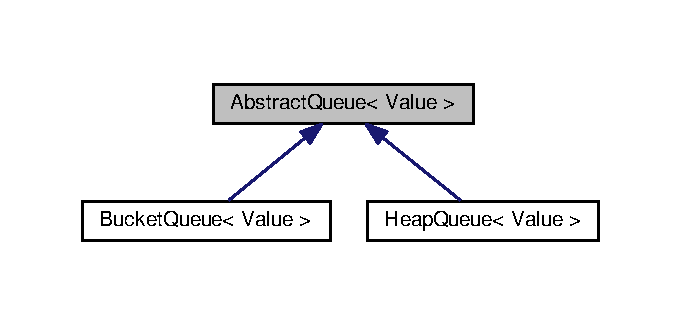
\includegraphics[width=327pt]{classAbstractQueue__inherit__graph}
\end{center}
\end{figure}
\subsection*{Public Types}
\begin{DoxyCompactItemize}
\item 
typedef std\-::pair$<$ int, Value $>$ \hyperlink{classAbstractQueue_abe60381528bc4cf9d4032f33f2ff6f3c}{Entry}
\end{DoxyCompactItemize}
\subsection*{Public Member Functions}
\begin{DoxyCompactItemize}
\item 
\hyperlink{classAbstractQueue_a65ca5c20345be92ce6b968715c5e9405}{Abstract\-Queue} ()
\item 
virtual \hyperlink{classAbstractQueue_a03cf0c0107bfdafb71c75872862e31fc}{$\sim$\-Abstract\-Queue} ()
\item 
virtual void \hyperlink{classAbstractQueue_af9268b0501749d8ab1b220a5db62a24e}{push} (int key, const Value \&value)=0
\item 
virtual \hyperlink{classAbstractQueue_abe60381528bc4cf9d4032f33f2ff6f3c}{Entry} \hyperlink{classAbstractQueue_aaec692216c729a7e7ca79b02a826cbf3}{pop} ()=0
\item 
virtual bool \hyperlink{classAbstractQueue_a38635110a147c0c1914e0f2f277a10de}{empty} () const =0
\item 
virtual void \hyperlink{classAbstractQueue_a2e976dcbc1ca3e97d05591cd466ff3e7}{clear} ()=0
\item 
virtual \hyperlink{classAbstractQueue}{Abstract\-Queue}$<$ Value $>$ $\ast$ \hyperlink{classAbstractQueue_a4c9793d6ec0442bbf806c2f57d6fd426}{convert\-\_\-if\-\_\-necessary} (int)
\item 
virtual void \hyperlink{classAbstractQueue_a2db622c67d66a0ee3d18e9e98145ece9}{add\-\_\-virtual\-\_\-pushes} (int num\-\_\-extra\-\_\-pushes)=0
\end{DoxyCompactItemize}


\subsection{Member Typedef Documentation}
\hypertarget{classAbstractQueue_abe60381528bc4cf9d4032f33f2ff6f3c}{\index{Abstract\-Queue@{Abstract\-Queue}!Entry@{Entry}}
\index{Entry@{Entry}!AbstractQueue@{Abstract\-Queue}}
\subsubsection[{Entry}]{\setlength{\rightskip}{0pt plus 5cm}template$<$typename Value$>$ typedef std\-::pair$<$int, Value$>$ {\bf Abstract\-Queue}$<$ Value $>$\-::{\bf Entry}}}\label{classAbstractQueue_abe60381528bc4cf9d4032f33f2ff6f3c}


\subsection{Constructor \& Destructor Documentation}
\hypertarget{classAbstractQueue_a65ca5c20345be92ce6b968715c5e9405}{\index{Abstract\-Queue@{Abstract\-Queue}!Abstract\-Queue@{Abstract\-Queue}}
\index{Abstract\-Queue@{Abstract\-Queue}!AbstractQueue@{Abstract\-Queue}}
\subsubsection[{Abstract\-Queue}]{\setlength{\rightskip}{0pt plus 5cm}template$<$typename Value$>$ {\bf Abstract\-Queue}$<$ Value $>$\-::{\bf Abstract\-Queue} (
\begin{DoxyParamCaption}
{}
\end{DoxyParamCaption}
)\hspace{0.3cm}{\ttfamily [inline]}}}\label{classAbstractQueue_a65ca5c20345be92ce6b968715c5e9405}
\hypertarget{classAbstractQueue_a03cf0c0107bfdafb71c75872862e31fc}{\index{Abstract\-Queue@{Abstract\-Queue}!$\sim$\-Abstract\-Queue@{$\sim$\-Abstract\-Queue}}
\index{$\sim$\-Abstract\-Queue@{$\sim$\-Abstract\-Queue}!AbstractQueue@{Abstract\-Queue}}
\subsubsection[{$\sim$\-Abstract\-Queue}]{\setlength{\rightskip}{0pt plus 5cm}template$<$typename Value$>$ virtual {\bf Abstract\-Queue}$<$ Value $>$\-::$\sim${\bf Abstract\-Queue} (
\begin{DoxyParamCaption}
{}
\end{DoxyParamCaption}
)\hspace{0.3cm}{\ttfamily [inline]}, {\ttfamily [virtual]}}}\label{classAbstractQueue_a03cf0c0107bfdafb71c75872862e31fc}


\subsection{Member Function Documentation}
\hypertarget{classAbstractQueue_a2db622c67d66a0ee3d18e9e98145ece9}{\index{Abstract\-Queue@{Abstract\-Queue}!add\-\_\-virtual\-\_\-pushes@{add\-\_\-virtual\-\_\-pushes}}
\index{add\-\_\-virtual\-\_\-pushes@{add\-\_\-virtual\-\_\-pushes}!AbstractQueue@{Abstract\-Queue}}
\subsubsection[{add\-\_\-virtual\-\_\-pushes}]{\setlength{\rightskip}{0pt plus 5cm}template$<$typename Value$>$ virtual void {\bf Abstract\-Queue}$<$ Value $>$\-::add\-\_\-virtual\-\_\-pushes (
\begin{DoxyParamCaption}
\item[{int}]{num\-\_\-extra\-\_\-pushes}
\end{DoxyParamCaption}
)\hspace{0.3cm}{\ttfamily [pure virtual]}}}\label{classAbstractQueue_a2db622c67d66a0ee3d18e9e98145ece9}


Implemented in \hyperlink{classBucketQueue_a362473bbbcf135376ec07be1b651b49d}{Bucket\-Queue$<$ Value $>$}, and \hyperlink{classHeapQueue_ad3d89c1e3f76c64ea10630bf5468c86f}{Heap\-Queue$<$ Value $>$}.

\hypertarget{classAbstractQueue_a2e976dcbc1ca3e97d05591cd466ff3e7}{\index{Abstract\-Queue@{Abstract\-Queue}!clear@{clear}}
\index{clear@{clear}!AbstractQueue@{Abstract\-Queue}}
\subsubsection[{clear}]{\setlength{\rightskip}{0pt plus 5cm}template$<$typename Value$>$ virtual void {\bf Abstract\-Queue}$<$ Value $>$\-::clear (
\begin{DoxyParamCaption}
{}
\end{DoxyParamCaption}
)\hspace{0.3cm}{\ttfamily [pure virtual]}}}\label{classAbstractQueue_a2e976dcbc1ca3e97d05591cd466ff3e7}


Implemented in \hyperlink{classBucketQueue_a749f5dc24bb6bb5754cb78f677b97d26}{Bucket\-Queue$<$ Value $>$}, and \hyperlink{classHeapQueue_af58d2cdb07e463b1d99013caf828df83}{Heap\-Queue$<$ Value $>$}.

\hypertarget{classAbstractQueue_a4c9793d6ec0442bbf806c2f57d6fd426}{\index{Abstract\-Queue@{Abstract\-Queue}!convert\-\_\-if\-\_\-necessary@{convert\-\_\-if\-\_\-necessary}}
\index{convert\-\_\-if\-\_\-necessary@{convert\-\_\-if\-\_\-necessary}!AbstractQueue@{Abstract\-Queue}}
\subsubsection[{convert\-\_\-if\-\_\-necessary}]{\setlength{\rightskip}{0pt plus 5cm}template$<$typename Value$>$ virtual {\bf Abstract\-Queue}$<$Value$>$$\ast$ {\bf Abstract\-Queue}$<$ Value $>$\-::convert\-\_\-if\-\_\-necessary (
\begin{DoxyParamCaption}
\item[{int}]{}
\end{DoxyParamCaption}
)\hspace{0.3cm}{\ttfamily [inline]}, {\ttfamily [virtual]}}}\label{classAbstractQueue_a4c9793d6ec0442bbf806c2f57d6fd426}


Reimplemented in \hyperlink{classBucketQueue_a4d56a716545e8a2a6e11481cd07d01ac}{Bucket\-Queue$<$ Value $>$}.

\hypertarget{classAbstractQueue_a38635110a147c0c1914e0f2f277a10de}{\index{Abstract\-Queue@{Abstract\-Queue}!empty@{empty}}
\index{empty@{empty}!AbstractQueue@{Abstract\-Queue}}
\subsubsection[{empty}]{\setlength{\rightskip}{0pt plus 5cm}template$<$typename Value$>$ virtual bool {\bf Abstract\-Queue}$<$ Value $>$\-::empty (
\begin{DoxyParamCaption}
{}
\end{DoxyParamCaption}
) const\hspace{0.3cm}{\ttfamily [pure virtual]}}}\label{classAbstractQueue_a38635110a147c0c1914e0f2f277a10de}


Implemented in \hyperlink{classBucketQueue_a3cf60e426df86413789dc19beee350b3}{Bucket\-Queue$<$ Value $>$}, and \hyperlink{classHeapQueue_a521d3e13a491f221947eee52a6ddfc0b}{Heap\-Queue$<$ Value $>$}.

\hypertarget{classAbstractQueue_aaec692216c729a7e7ca79b02a826cbf3}{\index{Abstract\-Queue@{Abstract\-Queue}!pop@{pop}}
\index{pop@{pop}!AbstractQueue@{Abstract\-Queue}}
\subsubsection[{pop}]{\setlength{\rightskip}{0pt plus 5cm}template$<$typename Value$>$ virtual {\bf Entry} {\bf Abstract\-Queue}$<$ Value $>$\-::pop (
\begin{DoxyParamCaption}
{}
\end{DoxyParamCaption}
)\hspace{0.3cm}{\ttfamily [pure virtual]}}}\label{classAbstractQueue_aaec692216c729a7e7ca79b02a826cbf3}


Implemented in \hyperlink{classBucketQueue_a2141b91ece1d2180d56ec74f07aa747e}{Bucket\-Queue$<$ Value $>$}, and \hyperlink{classHeapQueue_a6fcbe11f528e5ae359ae780c671d7125}{Heap\-Queue$<$ Value $>$}.

\hypertarget{classAbstractQueue_af9268b0501749d8ab1b220a5db62a24e}{\index{Abstract\-Queue@{Abstract\-Queue}!push@{push}}
\index{push@{push}!AbstractQueue@{Abstract\-Queue}}
\subsubsection[{push}]{\setlength{\rightskip}{0pt plus 5cm}template$<$typename Value$>$ virtual void {\bf Abstract\-Queue}$<$ Value $>$\-::push (
\begin{DoxyParamCaption}
\item[{int}]{key, }
\item[{const Value \&}]{value}
\end{DoxyParamCaption}
)\hspace{0.3cm}{\ttfamily [pure virtual]}}}\label{classAbstractQueue_af9268b0501749d8ab1b220a5db62a24e}


Implemented in \hyperlink{classBucketQueue_a1dc89d8bd4fd657dfc0218ca947f0d24}{Bucket\-Queue$<$ Value $>$}, and \hyperlink{classHeapQueue_a59850c8362a38865ee21b3db3d71f9e4}{Heap\-Queue$<$ Value $>$}.



The documentation for this class was generated from the following file\-:\begin{DoxyCompactItemize}
\item 
\hyperlink{priority__queue_8h}{priority\-\_\-queue.\-h}\end{DoxyCompactItemize}

\hypertarget{classAbstractTask}{\section{Abstract\-Task Class Reference}
\label{classAbstractTask}\index{Abstract\-Task@{Abstract\-Task}}
}


{\ttfamily \#include $<$abstract\-\_\-task.\-h$>$}



Inheritance diagram for Abstract\-Task\-:
\nopagebreak
\begin{figure}[H]
\begin{center}
\leavevmode
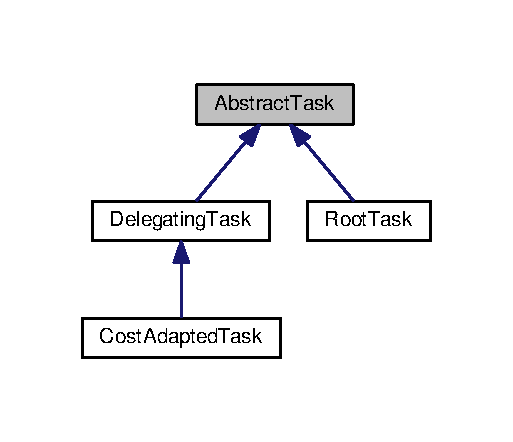
\includegraphics[width=246pt]{classAbstractTask__inherit__graph}
\end{center}
\end{figure}
\subsection*{Public Member Functions}
\begin{DoxyCompactItemize}
\item 
\hyperlink{classAbstractTask_a411b1b5beabae23f37f56cba1305a367}{Abstract\-Task} ()=default
\item 
virtual \hyperlink{classAbstractTask_a19d64eac973cb3521d861369737dd383}{$\sim$\-Abstract\-Task} ()=default
\item 
virtual int \hyperlink{classAbstractTask_ab0f878648c015fb918567403e80d4e4b}{get\-\_\-num\-\_\-variables} () const =0
\item 
virtual const std\-::string \& \hyperlink{classAbstractTask_acf846013bb556a5d5169b13a6bb879a5}{get\-\_\-variable\-\_\-name} (int var) const =0
\item 
virtual int \hyperlink{classAbstractTask_a8f229a999a431a27c75daad6bb86474e}{get\-\_\-variable\-\_\-domain\-\_\-size} (int var) const =0
\item 
virtual const std\-::string \& \hyperlink{classAbstractTask_a8ad9d3e97f1aa8fcde6cbc7844609c79}{get\-\_\-fact\-\_\-name} (int var, int value) const =0
\item 
virtual int \hyperlink{classAbstractTask_aeeb845c0f21bb3517d2ed79c8fdbf575}{get\-\_\-operator\-\_\-cost} (int index, bool is\-\_\-axiom) const =0
\item 
virtual const std\-::string \& \hyperlink{classAbstractTask_a528cea78d19468e616b2936aba22ea64}{get\-\_\-operator\-\_\-name} (int index, bool is\-\_\-axiom) const =0
\item 
virtual int \hyperlink{classAbstractTask_a616388eda808179e2dafcf8030348732}{get\-\_\-num\-\_\-operators} () const =0
\item 
virtual int \hyperlink{classAbstractTask_a2913e3d94adf9ce73ecf93a76efd64c0}{get\-\_\-num\-\_\-operator\-\_\-preconditions} (int index, bool is\-\_\-axiom) const =0
\item 
virtual std\-::pair$<$ int, int $>$ \hyperlink{classAbstractTask_a6d089445ffef1e87abdf2f989c275402}{get\-\_\-operator\-\_\-precondition} (int op\-\_\-index, int fact\-\_\-index, bool is\-\_\-axiom) const =0
\item 
virtual int \hyperlink{classAbstractTask_a101be8c121199154315a3539e59796b2}{get\-\_\-num\-\_\-operator\-\_\-effects} (int op\-\_\-index, bool is\-\_\-axiom) const =0
\item 
virtual int \hyperlink{classAbstractTask_a41642ad827682428ba1c099ecbde18ae}{get\-\_\-num\-\_\-operator\-\_\-effect\-\_\-conditions} (int op\-\_\-index, int eff\-\_\-index, bool is\-\_\-axiom) const =0
\item 
virtual std\-::pair$<$ int, int $>$ \hyperlink{classAbstractTask_a08f0a9248a99ccd0a1fdee940e0c0c4e}{get\-\_\-operator\-\_\-effect\-\_\-condition} (int op\-\_\-index, int eff\-\_\-index, int cond\-\_\-index, bool is\-\_\-axiom) const =0
\item 
virtual std\-::pair$<$ int, int $>$ \hyperlink{classAbstractTask_a4244a150e31b841e65f72ce89fa6ddad}{get\-\_\-operator\-\_\-effect} (int op\-\_\-index, int eff\-\_\-index, bool is\-\_\-axiom) const =0
\item 
virtual const \hyperlink{classGlobalOperator}{Global\-Operator} $\ast$ \hyperlink{classAbstractTask_ad0335ea9f89fa54b846780b55fad2545}{get\-\_\-global\-\_\-operator} (int index, bool is\-\_\-axiom) const =0
\item 
virtual int \hyperlink{classAbstractTask_a0e713664080d2a70036b6307779e7593}{get\-\_\-num\-\_\-axioms} () const =0
\item 
virtual int \hyperlink{classAbstractTask_a4e8335bdbfad228faf76e3c085d2ae4a}{get\-\_\-num\-\_\-goals} () const =0
\item 
virtual std\-::pair$<$ int, int $>$ \hyperlink{classAbstractTask_a737c7aca71dbf64b673236a0af4d8dde}{get\-\_\-goal\-\_\-fact} (int index) const =0
\item 
virtual std\-::vector$<$ int $>$ \hyperlink{classAbstractTask_a9de0ce6fb5349cc114cef522c54c595e}{get\-\_\-initial\-\_\-state\-\_\-values} () const =0
\item 
virtual std\-::vector$<$ int $>$ \hyperlink{classAbstractTask_a047d223704b817c72274f42c05fe3c7d}{get\-\_\-state\-\_\-values} (const \hyperlink{classGlobalState}{Global\-State} \&global\-\_\-state) const =0
\end{DoxyCompactItemize}


\subsection{Constructor \& Destructor Documentation}
\hypertarget{classAbstractTask_a411b1b5beabae23f37f56cba1305a367}{\index{Abstract\-Task@{Abstract\-Task}!Abstract\-Task@{Abstract\-Task}}
\index{Abstract\-Task@{Abstract\-Task}!AbstractTask@{Abstract\-Task}}
\subsubsection[{Abstract\-Task}]{\setlength{\rightskip}{0pt plus 5cm}Abstract\-Task\-::\-Abstract\-Task (
\begin{DoxyParamCaption}
{}
\end{DoxyParamCaption}
)\hspace{0.3cm}{\ttfamily [default]}}}\label{classAbstractTask_a411b1b5beabae23f37f56cba1305a367}
\hypertarget{classAbstractTask_a19d64eac973cb3521d861369737dd383}{\index{Abstract\-Task@{Abstract\-Task}!$\sim$\-Abstract\-Task@{$\sim$\-Abstract\-Task}}
\index{$\sim$\-Abstract\-Task@{$\sim$\-Abstract\-Task}!AbstractTask@{Abstract\-Task}}
\subsubsection[{$\sim$\-Abstract\-Task}]{\setlength{\rightskip}{0pt plus 5cm}virtual Abstract\-Task\-::$\sim$\-Abstract\-Task (
\begin{DoxyParamCaption}
{}
\end{DoxyParamCaption}
)\hspace{0.3cm}{\ttfamily [virtual]}, {\ttfamily [default]}}}\label{classAbstractTask_a19d64eac973cb3521d861369737dd383}


\subsection{Member Function Documentation}
\hypertarget{classAbstractTask_a8ad9d3e97f1aa8fcde6cbc7844609c79}{\index{Abstract\-Task@{Abstract\-Task}!get\-\_\-fact\-\_\-name@{get\-\_\-fact\-\_\-name}}
\index{get\-\_\-fact\-\_\-name@{get\-\_\-fact\-\_\-name}!AbstractTask@{Abstract\-Task}}
\subsubsection[{get\-\_\-fact\-\_\-name}]{\setlength{\rightskip}{0pt plus 5cm}virtual const std\-::string\& Abstract\-Task\-::get\-\_\-fact\-\_\-name (
\begin{DoxyParamCaption}
\item[{int}]{var, }
\item[{int}]{value}
\end{DoxyParamCaption}
) const\hspace{0.3cm}{\ttfamily [pure virtual]}}}\label{classAbstractTask_a8ad9d3e97f1aa8fcde6cbc7844609c79}


Implemented in \hyperlink{classDelegatingTask_aff6c956a3c936fcfeac368388e75c385}{Delegating\-Task}, and \hyperlink{classRootTask_a0e3e99e8c062751f261ec088ebb74a19}{Root\-Task}.

\hypertarget{classAbstractTask_ad0335ea9f89fa54b846780b55fad2545}{\index{Abstract\-Task@{Abstract\-Task}!get\-\_\-global\-\_\-operator@{get\-\_\-global\-\_\-operator}}
\index{get\-\_\-global\-\_\-operator@{get\-\_\-global\-\_\-operator}!AbstractTask@{Abstract\-Task}}
\subsubsection[{get\-\_\-global\-\_\-operator}]{\setlength{\rightskip}{0pt plus 5cm}virtual const {\bf Global\-Operator}$\ast$ Abstract\-Task\-::get\-\_\-global\-\_\-operator (
\begin{DoxyParamCaption}
\item[{int}]{index, }
\item[{bool}]{is\-\_\-axiom}
\end{DoxyParamCaption}
) const\hspace{0.3cm}{\ttfamily [pure virtual]}}}\label{classAbstractTask_ad0335ea9f89fa54b846780b55fad2545}


Implemented in \hyperlink{classDelegatingTask_a3807759260be9458378190ff25751b70}{Delegating\-Task}, and \hyperlink{classRootTask_a15e7790ef5ea158447e8cff9ff5343ea}{Root\-Task}.

\hypertarget{classAbstractTask_a737c7aca71dbf64b673236a0af4d8dde}{\index{Abstract\-Task@{Abstract\-Task}!get\-\_\-goal\-\_\-fact@{get\-\_\-goal\-\_\-fact}}
\index{get\-\_\-goal\-\_\-fact@{get\-\_\-goal\-\_\-fact}!AbstractTask@{Abstract\-Task}}
\subsubsection[{get\-\_\-goal\-\_\-fact}]{\setlength{\rightskip}{0pt plus 5cm}virtual std\-::pair$<$int, int$>$ Abstract\-Task\-::get\-\_\-goal\-\_\-fact (
\begin{DoxyParamCaption}
\item[{int}]{index}
\end{DoxyParamCaption}
) const\hspace{0.3cm}{\ttfamily [pure virtual]}}}\label{classAbstractTask_a737c7aca71dbf64b673236a0af4d8dde}


Implemented in \hyperlink{classDelegatingTask_a41ec9662ab3cd04af01e64a3805436fc}{Delegating\-Task}, and \hyperlink{classRootTask_a73ec00b3f1f0fe237dbea7ccff577e53}{Root\-Task}.

\hypertarget{classAbstractTask_a9de0ce6fb5349cc114cef522c54c595e}{\index{Abstract\-Task@{Abstract\-Task}!get\-\_\-initial\-\_\-state\-\_\-values@{get\-\_\-initial\-\_\-state\-\_\-values}}
\index{get\-\_\-initial\-\_\-state\-\_\-values@{get\-\_\-initial\-\_\-state\-\_\-values}!AbstractTask@{Abstract\-Task}}
\subsubsection[{get\-\_\-initial\-\_\-state\-\_\-values}]{\setlength{\rightskip}{0pt plus 5cm}virtual std\-::vector$<$int$>$ Abstract\-Task\-::get\-\_\-initial\-\_\-state\-\_\-values (
\begin{DoxyParamCaption}
{}
\end{DoxyParamCaption}
) const\hspace{0.3cm}{\ttfamily [pure virtual]}}}\label{classAbstractTask_a9de0ce6fb5349cc114cef522c54c595e}


Implemented in \hyperlink{classDelegatingTask_a62c81bb064e4d5e72f619f01e1e3f73c}{Delegating\-Task}, and \hyperlink{classRootTask_a125ca3ba7e42dd416d526d3232eef136}{Root\-Task}.

\hypertarget{classAbstractTask_a0e713664080d2a70036b6307779e7593}{\index{Abstract\-Task@{Abstract\-Task}!get\-\_\-num\-\_\-axioms@{get\-\_\-num\-\_\-axioms}}
\index{get\-\_\-num\-\_\-axioms@{get\-\_\-num\-\_\-axioms}!AbstractTask@{Abstract\-Task}}
\subsubsection[{get\-\_\-num\-\_\-axioms}]{\setlength{\rightskip}{0pt plus 5cm}virtual int Abstract\-Task\-::get\-\_\-num\-\_\-axioms (
\begin{DoxyParamCaption}
{}
\end{DoxyParamCaption}
) const\hspace{0.3cm}{\ttfamily [pure virtual]}}}\label{classAbstractTask_a0e713664080d2a70036b6307779e7593}


Implemented in \hyperlink{classDelegatingTask_af215094028d4c83cce4321e2cb2d011b}{Delegating\-Task}, and \hyperlink{classRootTask_a08ee54c9e9e9152bc6518ceb38309652}{Root\-Task}.

\hypertarget{classAbstractTask_a4e8335bdbfad228faf76e3c085d2ae4a}{\index{Abstract\-Task@{Abstract\-Task}!get\-\_\-num\-\_\-goals@{get\-\_\-num\-\_\-goals}}
\index{get\-\_\-num\-\_\-goals@{get\-\_\-num\-\_\-goals}!AbstractTask@{Abstract\-Task}}
\subsubsection[{get\-\_\-num\-\_\-goals}]{\setlength{\rightskip}{0pt plus 5cm}virtual int Abstract\-Task\-::get\-\_\-num\-\_\-goals (
\begin{DoxyParamCaption}
{}
\end{DoxyParamCaption}
) const\hspace{0.3cm}{\ttfamily [pure virtual]}}}\label{classAbstractTask_a4e8335bdbfad228faf76e3c085d2ae4a}


Implemented in \hyperlink{classDelegatingTask_a25fcb2255c42d684f89524de475f166e}{Delegating\-Task}, and \hyperlink{classRootTask_a082aa689a0166f76890babe2891cd977}{Root\-Task}.

\hypertarget{classAbstractTask_a41642ad827682428ba1c099ecbde18ae}{\index{Abstract\-Task@{Abstract\-Task}!get\-\_\-num\-\_\-operator\-\_\-effect\-\_\-conditions@{get\-\_\-num\-\_\-operator\-\_\-effect\-\_\-conditions}}
\index{get\-\_\-num\-\_\-operator\-\_\-effect\-\_\-conditions@{get\-\_\-num\-\_\-operator\-\_\-effect\-\_\-conditions}!AbstractTask@{Abstract\-Task}}
\subsubsection[{get\-\_\-num\-\_\-operator\-\_\-effect\-\_\-conditions}]{\setlength{\rightskip}{0pt plus 5cm}virtual int Abstract\-Task\-::get\-\_\-num\-\_\-operator\-\_\-effect\-\_\-conditions (
\begin{DoxyParamCaption}
\item[{int}]{op\-\_\-index, }
\item[{int}]{eff\-\_\-index, }
\item[{bool}]{is\-\_\-axiom}
\end{DoxyParamCaption}
) const\hspace{0.3cm}{\ttfamily [pure virtual]}}}\label{classAbstractTask_a41642ad827682428ba1c099ecbde18ae}


Implemented in \hyperlink{classDelegatingTask_a63119dfe36f38c8eaefa093a8d944b70}{Delegating\-Task}, and \hyperlink{classRootTask_aec7d32ea79fc430f6d280c74e5264e4d}{Root\-Task}.

\hypertarget{classAbstractTask_a101be8c121199154315a3539e59796b2}{\index{Abstract\-Task@{Abstract\-Task}!get\-\_\-num\-\_\-operator\-\_\-effects@{get\-\_\-num\-\_\-operator\-\_\-effects}}
\index{get\-\_\-num\-\_\-operator\-\_\-effects@{get\-\_\-num\-\_\-operator\-\_\-effects}!AbstractTask@{Abstract\-Task}}
\subsubsection[{get\-\_\-num\-\_\-operator\-\_\-effects}]{\setlength{\rightskip}{0pt plus 5cm}virtual int Abstract\-Task\-::get\-\_\-num\-\_\-operator\-\_\-effects (
\begin{DoxyParamCaption}
\item[{int}]{op\-\_\-index, }
\item[{bool}]{is\-\_\-axiom}
\end{DoxyParamCaption}
) const\hspace{0.3cm}{\ttfamily [pure virtual]}}}\label{classAbstractTask_a101be8c121199154315a3539e59796b2}


Implemented in \hyperlink{classDelegatingTask_af3f485cdbd1872e11ca53a47da104d35}{Delegating\-Task}, and \hyperlink{classRootTask_a74ec7d0968e42fcb0c5847509f518023}{Root\-Task}.

\hypertarget{classAbstractTask_a2913e3d94adf9ce73ecf93a76efd64c0}{\index{Abstract\-Task@{Abstract\-Task}!get\-\_\-num\-\_\-operator\-\_\-preconditions@{get\-\_\-num\-\_\-operator\-\_\-preconditions}}
\index{get\-\_\-num\-\_\-operator\-\_\-preconditions@{get\-\_\-num\-\_\-operator\-\_\-preconditions}!AbstractTask@{Abstract\-Task}}
\subsubsection[{get\-\_\-num\-\_\-operator\-\_\-preconditions}]{\setlength{\rightskip}{0pt plus 5cm}virtual int Abstract\-Task\-::get\-\_\-num\-\_\-operator\-\_\-preconditions (
\begin{DoxyParamCaption}
\item[{int}]{index, }
\item[{bool}]{is\-\_\-axiom}
\end{DoxyParamCaption}
) const\hspace{0.3cm}{\ttfamily [pure virtual]}}}\label{classAbstractTask_a2913e3d94adf9ce73ecf93a76efd64c0}


Implemented in \hyperlink{classDelegatingTask_a1b2ae69912faf4c5f58a13bd3f744dec}{Delegating\-Task}, and \hyperlink{classRootTask_ae78ed7674c9071317117cec0f19b026f}{Root\-Task}.

\hypertarget{classAbstractTask_a616388eda808179e2dafcf8030348732}{\index{Abstract\-Task@{Abstract\-Task}!get\-\_\-num\-\_\-operators@{get\-\_\-num\-\_\-operators}}
\index{get\-\_\-num\-\_\-operators@{get\-\_\-num\-\_\-operators}!AbstractTask@{Abstract\-Task}}
\subsubsection[{get\-\_\-num\-\_\-operators}]{\setlength{\rightskip}{0pt plus 5cm}virtual int Abstract\-Task\-::get\-\_\-num\-\_\-operators (
\begin{DoxyParamCaption}
{}
\end{DoxyParamCaption}
) const\hspace{0.3cm}{\ttfamily [pure virtual]}}}\label{classAbstractTask_a616388eda808179e2dafcf8030348732}


Implemented in \hyperlink{classDelegatingTask_a17d94e5b76add2569236c252ede36180}{Delegating\-Task}, and \hyperlink{classRootTask_a8df251f8be26777be878d309286ce1e7}{Root\-Task}.

\hypertarget{classAbstractTask_ab0f878648c015fb918567403e80d4e4b}{\index{Abstract\-Task@{Abstract\-Task}!get\-\_\-num\-\_\-variables@{get\-\_\-num\-\_\-variables}}
\index{get\-\_\-num\-\_\-variables@{get\-\_\-num\-\_\-variables}!AbstractTask@{Abstract\-Task}}
\subsubsection[{get\-\_\-num\-\_\-variables}]{\setlength{\rightskip}{0pt plus 5cm}virtual int Abstract\-Task\-::get\-\_\-num\-\_\-variables (
\begin{DoxyParamCaption}
{}
\end{DoxyParamCaption}
) const\hspace{0.3cm}{\ttfamily [pure virtual]}}}\label{classAbstractTask_ab0f878648c015fb918567403e80d4e4b}


Implemented in \hyperlink{classDelegatingTask_a1b3289d0d7b5567e38e06350788c1ece}{Delegating\-Task}, and \hyperlink{classRootTask_a4d49dd1233c035c319071a1977c6d0d4}{Root\-Task}.

\hypertarget{classAbstractTask_aeeb845c0f21bb3517d2ed79c8fdbf575}{\index{Abstract\-Task@{Abstract\-Task}!get\-\_\-operator\-\_\-cost@{get\-\_\-operator\-\_\-cost}}
\index{get\-\_\-operator\-\_\-cost@{get\-\_\-operator\-\_\-cost}!AbstractTask@{Abstract\-Task}}
\subsubsection[{get\-\_\-operator\-\_\-cost}]{\setlength{\rightskip}{0pt plus 5cm}virtual int Abstract\-Task\-::get\-\_\-operator\-\_\-cost (
\begin{DoxyParamCaption}
\item[{int}]{index, }
\item[{bool}]{is\-\_\-axiom}
\end{DoxyParamCaption}
) const\hspace{0.3cm}{\ttfamily [pure virtual]}}}\label{classAbstractTask_aeeb845c0f21bb3517d2ed79c8fdbf575}


Implemented in \hyperlink{classCostAdaptedTask_a931aa2a13aaff9410582e903f5cfbc9d}{Cost\-Adapted\-Task}, \hyperlink{classDelegatingTask_a88352a7f751b06d0bd5302388d7ec377}{Delegating\-Task}, and \hyperlink{classRootTask_a37a97a51a64ddc05e85d3252c685392a}{Root\-Task}.

\hypertarget{classAbstractTask_a4244a150e31b841e65f72ce89fa6ddad}{\index{Abstract\-Task@{Abstract\-Task}!get\-\_\-operator\-\_\-effect@{get\-\_\-operator\-\_\-effect}}
\index{get\-\_\-operator\-\_\-effect@{get\-\_\-operator\-\_\-effect}!AbstractTask@{Abstract\-Task}}
\subsubsection[{get\-\_\-operator\-\_\-effect}]{\setlength{\rightskip}{0pt plus 5cm}virtual std\-::pair$<$int, int$>$ Abstract\-Task\-::get\-\_\-operator\-\_\-effect (
\begin{DoxyParamCaption}
\item[{int}]{op\-\_\-index, }
\item[{int}]{eff\-\_\-index, }
\item[{bool}]{is\-\_\-axiom}
\end{DoxyParamCaption}
) const\hspace{0.3cm}{\ttfamily [pure virtual]}}}\label{classAbstractTask_a4244a150e31b841e65f72ce89fa6ddad}


Implemented in \hyperlink{classDelegatingTask_a3f2571a63c2b22327df586e5a9d0df3e}{Delegating\-Task}, and \hyperlink{classRootTask_a7880bd37c8750a2f7045440de8d9e39e}{Root\-Task}.

\hypertarget{classAbstractTask_a08f0a9248a99ccd0a1fdee940e0c0c4e}{\index{Abstract\-Task@{Abstract\-Task}!get\-\_\-operator\-\_\-effect\-\_\-condition@{get\-\_\-operator\-\_\-effect\-\_\-condition}}
\index{get\-\_\-operator\-\_\-effect\-\_\-condition@{get\-\_\-operator\-\_\-effect\-\_\-condition}!AbstractTask@{Abstract\-Task}}
\subsubsection[{get\-\_\-operator\-\_\-effect\-\_\-condition}]{\setlength{\rightskip}{0pt plus 5cm}virtual std\-::pair$<$int, int$>$ Abstract\-Task\-::get\-\_\-operator\-\_\-effect\-\_\-condition (
\begin{DoxyParamCaption}
\item[{int}]{op\-\_\-index, }
\item[{int}]{eff\-\_\-index, }
\item[{int}]{cond\-\_\-index, }
\item[{bool}]{is\-\_\-axiom}
\end{DoxyParamCaption}
) const\hspace{0.3cm}{\ttfamily [pure virtual]}}}\label{classAbstractTask_a08f0a9248a99ccd0a1fdee940e0c0c4e}


Implemented in \hyperlink{classDelegatingTask_aaabb1108e7759110b1125482ba528e74}{Delegating\-Task}, and \hyperlink{classRootTask_aa37d8174fe1d2e62642502e7483b88b2}{Root\-Task}.

\hypertarget{classAbstractTask_a528cea78d19468e616b2936aba22ea64}{\index{Abstract\-Task@{Abstract\-Task}!get\-\_\-operator\-\_\-name@{get\-\_\-operator\-\_\-name}}
\index{get\-\_\-operator\-\_\-name@{get\-\_\-operator\-\_\-name}!AbstractTask@{Abstract\-Task}}
\subsubsection[{get\-\_\-operator\-\_\-name}]{\setlength{\rightskip}{0pt plus 5cm}virtual const std\-::string\& Abstract\-Task\-::get\-\_\-operator\-\_\-name (
\begin{DoxyParamCaption}
\item[{int}]{index, }
\item[{bool}]{is\-\_\-axiom}
\end{DoxyParamCaption}
) const\hspace{0.3cm}{\ttfamily [pure virtual]}}}\label{classAbstractTask_a528cea78d19468e616b2936aba22ea64}


Implemented in \hyperlink{classDelegatingTask_af0069346a9bf01c82e6ca9f5220f0f1d}{Delegating\-Task}, and \hyperlink{classRootTask_adb7ac227f8595146614ab51d89793765}{Root\-Task}.

\hypertarget{classAbstractTask_a6d089445ffef1e87abdf2f989c275402}{\index{Abstract\-Task@{Abstract\-Task}!get\-\_\-operator\-\_\-precondition@{get\-\_\-operator\-\_\-precondition}}
\index{get\-\_\-operator\-\_\-precondition@{get\-\_\-operator\-\_\-precondition}!AbstractTask@{Abstract\-Task}}
\subsubsection[{get\-\_\-operator\-\_\-precondition}]{\setlength{\rightskip}{0pt plus 5cm}virtual std\-::pair$<$int, int$>$ Abstract\-Task\-::get\-\_\-operator\-\_\-precondition (
\begin{DoxyParamCaption}
\item[{int}]{op\-\_\-index, }
\item[{int}]{fact\-\_\-index, }
\item[{bool}]{is\-\_\-axiom}
\end{DoxyParamCaption}
) const\hspace{0.3cm}{\ttfamily [pure virtual]}}}\label{classAbstractTask_a6d089445ffef1e87abdf2f989c275402}


Implemented in \hyperlink{classDelegatingTask_a20b4112f42c5cabdb2b578db176b0d1f}{Delegating\-Task}, and \hyperlink{classRootTask_aa9f9d67cc6824ccd7008666bb53262e4}{Root\-Task}.

\hypertarget{classAbstractTask_a047d223704b817c72274f42c05fe3c7d}{\index{Abstract\-Task@{Abstract\-Task}!get\-\_\-state\-\_\-values@{get\-\_\-state\-\_\-values}}
\index{get\-\_\-state\-\_\-values@{get\-\_\-state\-\_\-values}!AbstractTask@{Abstract\-Task}}
\subsubsection[{get\-\_\-state\-\_\-values}]{\setlength{\rightskip}{0pt plus 5cm}virtual std\-::vector$<$int$>$ Abstract\-Task\-::get\-\_\-state\-\_\-values (
\begin{DoxyParamCaption}
\item[{const {\bf Global\-State} \&}]{global\-\_\-state}
\end{DoxyParamCaption}
) const\hspace{0.3cm}{\ttfamily [pure virtual]}}}\label{classAbstractTask_a047d223704b817c72274f42c05fe3c7d}


Implemented in \hyperlink{classDelegatingTask_a04ac3437f7f4ae171190ef5972d8d16e}{Delegating\-Task}, and \hyperlink{classRootTask_af1a6f15dae32109865b022238e0bd4d0}{Root\-Task}.

\hypertarget{classAbstractTask_a8f229a999a431a27c75daad6bb86474e}{\index{Abstract\-Task@{Abstract\-Task}!get\-\_\-variable\-\_\-domain\-\_\-size@{get\-\_\-variable\-\_\-domain\-\_\-size}}
\index{get\-\_\-variable\-\_\-domain\-\_\-size@{get\-\_\-variable\-\_\-domain\-\_\-size}!AbstractTask@{Abstract\-Task}}
\subsubsection[{get\-\_\-variable\-\_\-domain\-\_\-size}]{\setlength{\rightskip}{0pt plus 5cm}virtual int Abstract\-Task\-::get\-\_\-variable\-\_\-domain\-\_\-size (
\begin{DoxyParamCaption}
\item[{int}]{var}
\end{DoxyParamCaption}
) const\hspace{0.3cm}{\ttfamily [pure virtual]}}}\label{classAbstractTask_a8f229a999a431a27c75daad6bb86474e}


Implemented in \hyperlink{classDelegatingTask_a2744ecccb1f245e7d2197e353d79e632}{Delegating\-Task}, and \hyperlink{classRootTask_a268a95d20e865b066424b6f5a656c60a}{Root\-Task}.

\hypertarget{classAbstractTask_acf846013bb556a5d5169b13a6bb879a5}{\index{Abstract\-Task@{Abstract\-Task}!get\-\_\-variable\-\_\-name@{get\-\_\-variable\-\_\-name}}
\index{get\-\_\-variable\-\_\-name@{get\-\_\-variable\-\_\-name}!AbstractTask@{Abstract\-Task}}
\subsubsection[{get\-\_\-variable\-\_\-name}]{\setlength{\rightskip}{0pt plus 5cm}virtual const std\-::string\& Abstract\-Task\-::get\-\_\-variable\-\_\-name (
\begin{DoxyParamCaption}
\item[{int}]{var}
\end{DoxyParamCaption}
) const\hspace{0.3cm}{\ttfamily [pure virtual]}}}\label{classAbstractTask_acf846013bb556a5d5169b13a6bb879a5}


Implemented in \hyperlink{classDelegatingTask_a6d0d9b3cfb2eac8f46dbbcbb2284dab3}{Delegating\-Task}, and \hyperlink{classRootTask_a156cccfcdc7ad59e8792409b0f06ad1d}{Root\-Task}.



The documentation for this class was generated from the following file\-:\begin{DoxyCompactItemize}
\item 
\hyperlink{abstract__task_8h}{abstract\-\_\-task.\-h}\end{DoxyCompactItemize}

\hypertarget{classAdaptiveQueue}{\section{Adaptive\-Queue$<$ Value $>$ Class Template Reference}
\label{classAdaptiveQueue}\index{Adaptive\-Queue$<$ Value $>$@{Adaptive\-Queue$<$ Value $>$}}
}


{\ttfamily \#include $<$priority\-\_\-queue.\-h$>$}

\subsection*{Public Types}
\begin{DoxyCompactItemize}
\item 
typedef std\-::pair$<$ int, Value $>$ \hyperlink{classAdaptiveQueue_a72a962211b8c52208580935d01bcaaa4}{Entry}
\end{DoxyCompactItemize}
\subsection*{Public Member Functions}
\begin{DoxyCompactItemize}
\item 
\hyperlink{classAdaptiveQueue_a447601821d0fe5dafa3cca82c015ddc7}{Adaptive\-Queue} ()
\item 
\hyperlink{classAdaptiveQueue_a94bc77945a01b338061c014d6be3cd7c}{$\sim$\-Adaptive\-Queue} ()
\item 
void \hyperlink{classAdaptiveQueue_a6308ad70f0102672324c20d502036aa5}{push} (int key, const Value \&value)
\item 
\hyperlink{classAdaptiveQueue_a72a962211b8c52208580935d01bcaaa4}{Entry} \hyperlink{classAdaptiveQueue_ae188c14bef82f7b833f21940c6c0fa8a}{pop} ()
\item 
bool \hyperlink{classAdaptiveQueue_a4111d42beeb98471e5e1fd240f8dc0d3}{empty} () const 
\item 
void \hyperlink{classAdaptiveQueue_adea90ba174e69361f492636e49d49343}{clear} ()
\item 
void \hyperlink{classAdaptiveQueue_a08008edc6ba3953ea741dbcb5cda01f0}{add\-\_\-virtual\-\_\-pushes} (int num\-\_\-extra\-\_\-pushes)
\end{DoxyCompactItemize}


\subsection{Member Typedef Documentation}
\hypertarget{classAdaptiveQueue_a72a962211b8c52208580935d01bcaaa4}{\index{Adaptive\-Queue@{Adaptive\-Queue}!Entry@{Entry}}
\index{Entry@{Entry}!AdaptiveQueue@{Adaptive\-Queue}}
\subsubsection[{Entry}]{\setlength{\rightskip}{0pt plus 5cm}template$<$typename Value$>$ typedef std\-::pair$<$int, Value$>$ {\bf Adaptive\-Queue}$<$ Value $>$\-::{\bf Entry}}}\label{classAdaptiveQueue_a72a962211b8c52208580935d01bcaaa4}


\subsection{Constructor \& Destructor Documentation}
\hypertarget{classAdaptiveQueue_a447601821d0fe5dafa3cca82c015ddc7}{\index{Adaptive\-Queue@{Adaptive\-Queue}!Adaptive\-Queue@{Adaptive\-Queue}}
\index{Adaptive\-Queue@{Adaptive\-Queue}!AdaptiveQueue@{Adaptive\-Queue}}
\subsubsection[{Adaptive\-Queue}]{\setlength{\rightskip}{0pt plus 5cm}template$<$typename Value$>$ {\bf Adaptive\-Queue}$<$ Value $>$\-::{\bf Adaptive\-Queue} (
\begin{DoxyParamCaption}
{}
\end{DoxyParamCaption}
)\hspace{0.3cm}{\ttfamily [inline]}}}\label{classAdaptiveQueue_a447601821d0fe5dafa3cca82c015ddc7}
\hypertarget{classAdaptiveQueue_a94bc77945a01b338061c014d6be3cd7c}{\index{Adaptive\-Queue@{Adaptive\-Queue}!$\sim$\-Adaptive\-Queue@{$\sim$\-Adaptive\-Queue}}
\index{$\sim$\-Adaptive\-Queue@{$\sim$\-Adaptive\-Queue}!AdaptiveQueue@{Adaptive\-Queue}}
\subsubsection[{$\sim$\-Adaptive\-Queue}]{\setlength{\rightskip}{0pt plus 5cm}template$<$typename Value$>$ {\bf Adaptive\-Queue}$<$ Value $>$\-::$\sim${\bf Adaptive\-Queue} (
\begin{DoxyParamCaption}
{}
\end{DoxyParamCaption}
)\hspace{0.3cm}{\ttfamily [inline]}}}\label{classAdaptiveQueue_a94bc77945a01b338061c014d6be3cd7c}


\subsection{Member Function Documentation}
\hypertarget{classAdaptiveQueue_a08008edc6ba3953ea741dbcb5cda01f0}{\index{Adaptive\-Queue@{Adaptive\-Queue}!add\-\_\-virtual\-\_\-pushes@{add\-\_\-virtual\-\_\-pushes}}
\index{add\-\_\-virtual\-\_\-pushes@{add\-\_\-virtual\-\_\-pushes}!AdaptiveQueue@{Adaptive\-Queue}}
\subsubsection[{add\-\_\-virtual\-\_\-pushes}]{\setlength{\rightskip}{0pt plus 5cm}template$<$typename Value$>$ void {\bf Adaptive\-Queue}$<$ Value $>$\-::add\-\_\-virtual\-\_\-pushes (
\begin{DoxyParamCaption}
\item[{int}]{num\-\_\-extra\-\_\-pushes}
\end{DoxyParamCaption}
)\hspace{0.3cm}{\ttfamily [inline]}}}\label{classAdaptiveQueue_a08008edc6ba3953ea741dbcb5cda01f0}
\hypertarget{classAdaptiveQueue_adea90ba174e69361f492636e49d49343}{\index{Adaptive\-Queue@{Adaptive\-Queue}!clear@{clear}}
\index{clear@{clear}!AdaptiveQueue@{Adaptive\-Queue}}
\subsubsection[{clear}]{\setlength{\rightskip}{0pt plus 5cm}template$<$typename Value$>$ void {\bf Adaptive\-Queue}$<$ Value $>$\-::clear (
\begin{DoxyParamCaption}
{}
\end{DoxyParamCaption}
)\hspace{0.3cm}{\ttfamily [inline]}}}\label{classAdaptiveQueue_adea90ba174e69361f492636e49d49343}
\hypertarget{classAdaptiveQueue_a4111d42beeb98471e5e1fd240f8dc0d3}{\index{Adaptive\-Queue@{Adaptive\-Queue}!empty@{empty}}
\index{empty@{empty}!AdaptiveQueue@{Adaptive\-Queue}}
\subsubsection[{empty}]{\setlength{\rightskip}{0pt plus 5cm}template$<$typename Value$>$ bool {\bf Adaptive\-Queue}$<$ Value $>$\-::empty (
\begin{DoxyParamCaption}
{}
\end{DoxyParamCaption}
) const\hspace{0.3cm}{\ttfamily [inline]}}}\label{classAdaptiveQueue_a4111d42beeb98471e5e1fd240f8dc0d3}
\hypertarget{classAdaptiveQueue_ae188c14bef82f7b833f21940c6c0fa8a}{\index{Adaptive\-Queue@{Adaptive\-Queue}!pop@{pop}}
\index{pop@{pop}!AdaptiveQueue@{Adaptive\-Queue}}
\subsubsection[{pop}]{\setlength{\rightskip}{0pt plus 5cm}template$<$typename Value$>$ {\bf Entry} {\bf Adaptive\-Queue}$<$ Value $>$\-::pop (
\begin{DoxyParamCaption}
{}
\end{DoxyParamCaption}
)\hspace{0.3cm}{\ttfamily [inline]}}}\label{classAdaptiveQueue_ae188c14bef82f7b833f21940c6c0fa8a}
\hypertarget{classAdaptiveQueue_a6308ad70f0102672324c20d502036aa5}{\index{Adaptive\-Queue@{Adaptive\-Queue}!push@{push}}
\index{push@{push}!AdaptiveQueue@{Adaptive\-Queue}}
\subsubsection[{push}]{\setlength{\rightskip}{0pt plus 5cm}template$<$typename Value$>$ void {\bf Adaptive\-Queue}$<$ Value $>$\-::push (
\begin{DoxyParamCaption}
\item[{int}]{key, }
\item[{const Value \&}]{value}
\end{DoxyParamCaption}
)\hspace{0.3cm}{\ttfamily [inline]}}}\label{classAdaptiveQueue_a6308ad70f0102672324c20d502036aa5}


The documentation for this class was generated from the following file\-:\begin{DoxyCompactItemize}
\item 
\hyperlink{priority__queue_8h}{priority\-\_\-queue.\-h}\end{DoxyCompactItemize}

\hypertarget{classAdditiveHeuristic}{\section{Additive\-Heuristic Class Reference}
\label{classAdditiveHeuristic}\index{Additive\-Heuristic@{Additive\-Heuristic}}
}


{\ttfamily \#include $<$additive\-\_\-heuristic.\-h$>$}



Inheritance diagram for Additive\-Heuristic\-:
\nopagebreak
\begin{figure}[H]
\begin{center}
\leavevmode
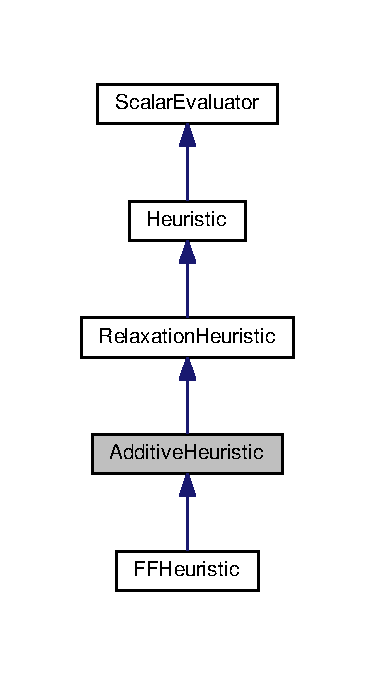
\includegraphics[width=180pt]{classAdditiveHeuristic__inherit__graph}
\end{center}
\end{figure}


Collaboration diagram for Additive\-Heuristic\-:
\nopagebreak
\begin{figure}[H]
\begin{center}
\leavevmode
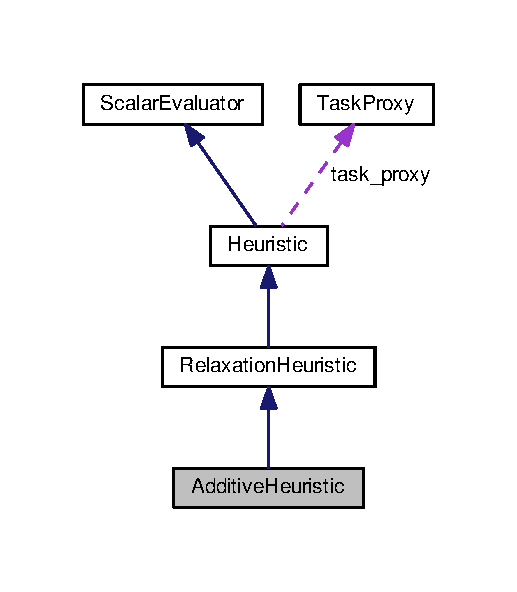
\includegraphics[width=248pt]{classAdditiveHeuristic__coll__graph}
\end{center}
\end{figure}
\subsection*{Public Member Functions}
\begin{DoxyCompactItemize}
\item 
\hyperlink{classAdditiveHeuristic_acd989fb614ffd4bb4523fa01fc9e0a0d}{Additive\-Heuristic} (const \hyperlink{classOptions}{Options} \&options)
\item 
\hyperlink{classAdditiveHeuristic_ae59ba3ba74b38fb9ef3b6d35be6e2c48}{$\sim$\-Additive\-Heuristic} ()
\end{DoxyCompactItemize}
\subsection*{Protected Member Functions}
\begin{DoxyCompactItemize}
\item 
virtual void \hyperlink{classAdditiveHeuristic_a4c952cd832e8dd3ea364d8cac379ebbc}{initialize} ()
\item 
virtual int \hyperlink{classAdditiveHeuristic_ad2c71f6c5198a7276b7892e2d0a5bca8}{compute\-\_\-heuristic} (const \hyperlink{classGlobalState}{Global\-State} \&global\-\_\-state)
\item 
int \hyperlink{classAdditiveHeuristic_a704d2da5f869d2e0b3ed726b87130343}{compute\-\_\-add\-\_\-and\-\_\-ff} (const \hyperlink{classState}{State} \&state)
\end{DoxyCompactItemize}
\subsection*{Additional Inherited Members}


\subsection{Constructor \& Destructor Documentation}
\hypertarget{classAdditiveHeuristic_acd989fb614ffd4bb4523fa01fc9e0a0d}{\index{Additive\-Heuristic@{Additive\-Heuristic}!Additive\-Heuristic@{Additive\-Heuristic}}
\index{Additive\-Heuristic@{Additive\-Heuristic}!AdditiveHeuristic@{Additive\-Heuristic}}
\subsubsection[{Additive\-Heuristic}]{\setlength{\rightskip}{0pt plus 5cm}Additive\-Heuristic\-::\-Additive\-Heuristic (
\begin{DoxyParamCaption}
\item[{const {\bf Options} \&}]{options}
\end{DoxyParamCaption}
)}}\label{classAdditiveHeuristic_acd989fb614ffd4bb4523fa01fc9e0a0d}
\hypertarget{classAdditiveHeuristic_ae59ba3ba74b38fb9ef3b6d35be6e2c48}{\index{Additive\-Heuristic@{Additive\-Heuristic}!$\sim$\-Additive\-Heuristic@{$\sim$\-Additive\-Heuristic}}
\index{$\sim$\-Additive\-Heuristic@{$\sim$\-Additive\-Heuristic}!AdditiveHeuristic@{Additive\-Heuristic}}
\subsubsection[{$\sim$\-Additive\-Heuristic}]{\setlength{\rightskip}{0pt plus 5cm}Additive\-Heuristic\-::$\sim$\-Additive\-Heuristic (
\begin{DoxyParamCaption}
{}
\end{DoxyParamCaption}
)}}\label{classAdditiveHeuristic_ae59ba3ba74b38fb9ef3b6d35be6e2c48}


\subsection{Member Function Documentation}
\hypertarget{classAdditiveHeuristic_a704d2da5f869d2e0b3ed726b87130343}{\index{Additive\-Heuristic@{Additive\-Heuristic}!compute\-\_\-add\-\_\-and\-\_\-ff@{compute\-\_\-add\-\_\-and\-\_\-ff}}
\index{compute\-\_\-add\-\_\-and\-\_\-ff@{compute\-\_\-add\-\_\-and\-\_\-ff}!AdditiveHeuristic@{Additive\-Heuristic}}
\subsubsection[{compute\-\_\-add\-\_\-and\-\_\-ff}]{\setlength{\rightskip}{0pt plus 5cm}int Additive\-Heuristic\-::compute\-\_\-add\-\_\-and\-\_\-ff (
\begin{DoxyParamCaption}
\item[{const {\bf State} \&}]{state}
\end{DoxyParamCaption}
)\hspace{0.3cm}{\ttfamily [protected]}}}\label{classAdditiveHeuristic_a704d2da5f869d2e0b3ed726b87130343}
\hypertarget{classAdditiveHeuristic_ad2c71f6c5198a7276b7892e2d0a5bca8}{\index{Additive\-Heuristic@{Additive\-Heuristic}!compute\-\_\-heuristic@{compute\-\_\-heuristic}}
\index{compute\-\_\-heuristic@{compute\-\_\-heuristic}!AdditiveHeuristic@{Additive\-Heuristic}}
\subsubsection[{compute\-\_\-heuristic}]{\setlength{\rightskip}{0pt plus 5cm}int Additive\-Heuristic\-::compute\-\_\-heuristic (
\begin{DoxyParamCaption}
\item[{const {\bf Global\-State} \&}]{global\-\_\-state}
\end{DoxyParamCaption}
)\hspace{0.3cm}{\ttfamily [protected]}, {\ttfamily [virtual]}}}\label{classAdditiveHeuristic_ad2c71f6c5198a7276b7892e2d0a5bca8}


Implements \hyperlink{classRelaxationHeuristic_a7455dfe0d43241c0f0769db91ee87ec3}{Relaxation\-Heuristic}.



Reimplemented in \hyperlink{classFFHeuristic_a0b3c97fce6e723cf8f73ee9da0a58a79}{F\-F\-Heuristic}.



Here is the call graph for this function\-:
\nopagebreak
\begin{figure}[H]
\begin{center}
\leavevmode
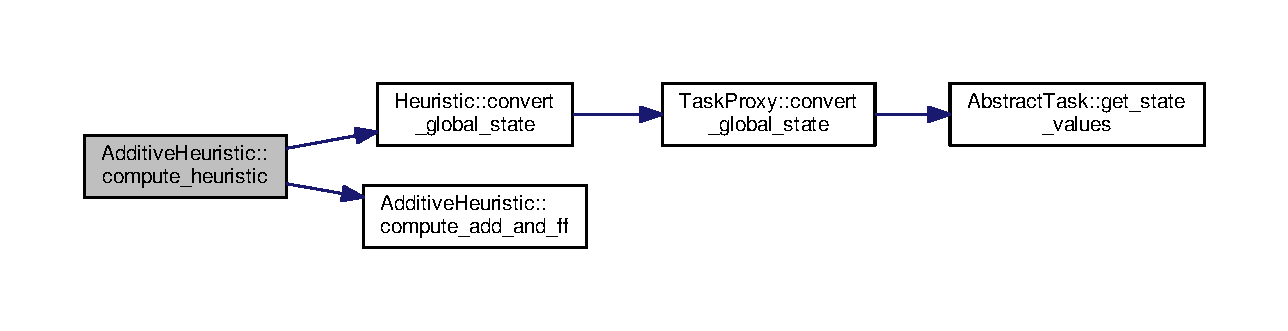
\includegraphics[width=350pt]{classAdditiveHeuristic_ad2c71f6c5198a7276b7892e2d0a5bca8_cgraph}
\end{center}
\end{figure}


\hypertarget{classAdditiveHeuristic_a4c952cd832e8dd3ea364d8cac379ebbc}{\index{Additive\-Heuristic@{Additive\-Heuristic}!initialize@{initialize}}
\index{initialize@{initialize}!AdditiveHeuristic@{Additive\-Heuristic}}
\subsubsection[{initialize}]{\setlength{\rightskip}{0pt plus 5cm}void Additive\-Heuristic\-::initialize (
\begin{DoxyParamCaption}
{}
\end{DoxyParamCaption}
)\hspace{0.3cm}{\ttfamily [protected]}, {\ttfamily [virtual]}}}\label{classAdditiveHeuristic_a4c952cd832e8dd3ea364d8cac379ebbc}


Reimplemented from \hyperlink{classRelaxationHeuristic_aa34cc79d9e5e3e9aff4c4ed1b03a853e}{Relaxation\-Heuristic}.



Reimplemented in \hyperlink{classFFHeuristic_ad17e4f428e5c4fc89d4e0de8e8ed6d80}{F\-F\-Heuristic}.



Here is the call graph for this function\-:
\nopagebreak
\begin{figure}[H]
\begin{center}
\leavevmode
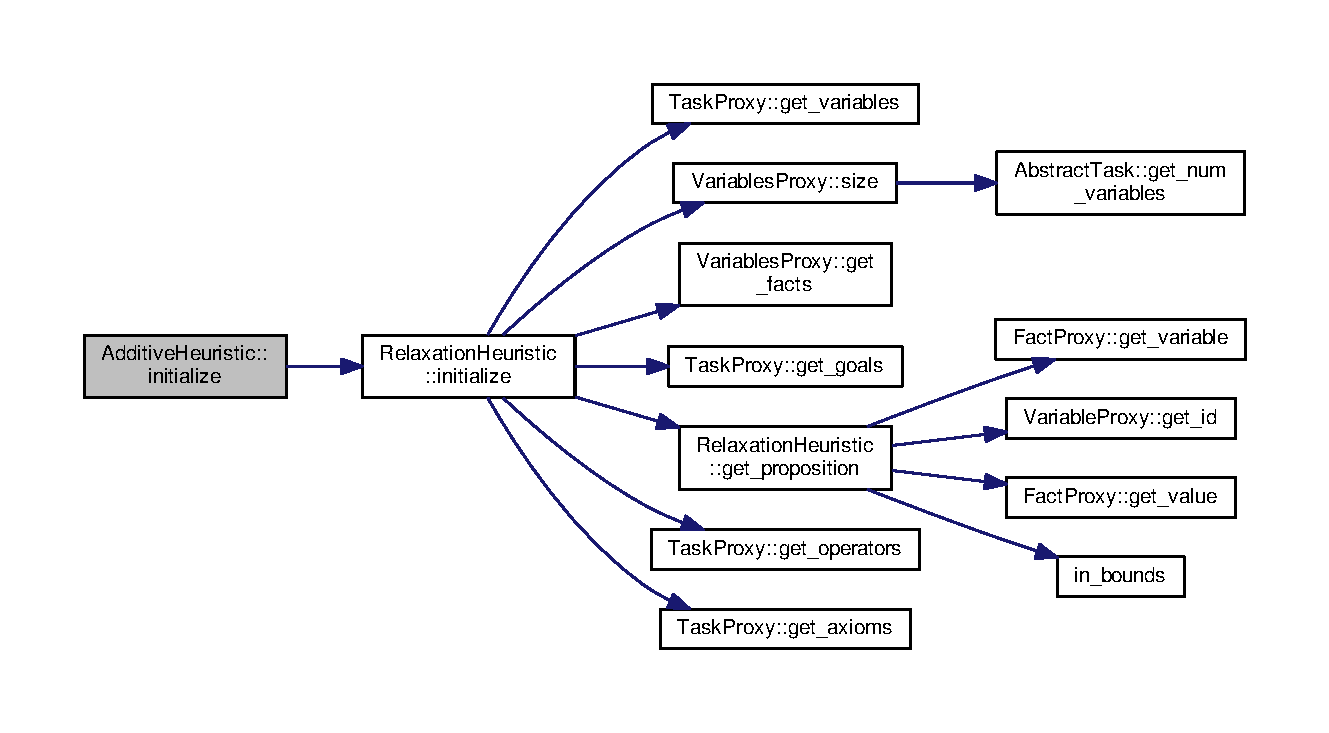
\includegraphics[width=350pt]{classAdditiveHeuristic_a4c952cd832e8dd3ea364d8cac379ebbc_cgraph}
\end{center}
\end{figure}




The documentation for this class was generated from the following files\-:\begin{DoxyCompactItemize}
\item 
\hyperlink{additive__heuristic_8h}{additive\-\_\-heuristic.\-h}\item 
\hyperlink{additive__heuristic_8cc}{additive\-\_\-heuristic.\-cc}\end{DoxyCompactItemize}

\hypertarget{structArgError}{\section{Arg\-Error Struct Reference}
\label{structArgError}\index{Arg\-Error@{Arg\-Error}}
}


{\ttfamily \#include $<$option\-\_\-parser\-\_\-util.\-h$>$}

\subsection*{Public Member Functions}
\begin{DoxyCompactItemize}
\item 
\hyperlink{structArgError_a19630d2915344226977912a02f98ea5f}{Arg\-Error} (std\-::string \hyperlink{structArgError_a855e517b2ab5cd92851ca4e3fac34d26}{msg})
\end{DoxyCompactItemize}
\subsection*{Public Attributes}
\begin{DoxyCompactItemize}
\item 
std\-::string \hyperlink{structArgError_a855e517b2ab5cd92851ca4e3fac34d26}{msg}
\end{DoxyCompactItemize}
\subsection*{Friends}
\begin{DoxyCompactItemize}
\item 
std\-::ostream \& \hyperlink{structArgError_a88335e47551a0b99303654514224b3f2}{operator$<$$<$} (std\-::ostream \&out, const \hyperlink{structArgError}{Arg\-Error} \&err)
\end{DoxyCompactItemize}


\subsection{Constructor \& Destructor Documentation}
\hypertarget{structArgError_a19630d2915344226977912a02f98ea5f}{\index{Arg\-Error@{Arg\-Error}!Arg\-Error@{Arg\-Error}}
\index{Arg\-Error@{Arg\-Error}!ArgError@{Arg\-Error}}
\subsubsection[{Arg\-Error}]{\setlength{\rightskip}{0pt plus 5cm}Arg\-Error\-::\-Arg\-Error (
\begin{DoxyParamCaption}
\item[{std\-::string}]{msg}
\end{DoxyParamCaption}
)}}\label{structArgError_a19630d2915344226977912a02f98ea5f}


\subsection{Friends And Related Function Documentation}
\hypertarget{structArgError_a88335e47551a0b99303654514224b3f2}{\index{Arg\-Error@{Arg\-Error}!operator$<$$<$@{operator$<$$<$}}
\index{operator$<$$<$@{operator$<$$<$}!ArgError@{Arg\-Error}}
\subsubsection[{operator$<$$<$}]{\setlength{\rightskip}{0pt plus 5cm}std\-::ostream\& operator$<$$<$ (
\begin{DoxyParamCaption}
\item[{std\-::ostream \&}]{out, }
\item[{const {\bf Arg\-Error} \&}]{err}
\end{DoxyParamCaption}
)\hspace{0.3cm}{\ttfamily [friend]}}}\label{structArgError_a88335e47551a0b99303654514224b3f2}


\subsection{Member Data Documentation}
\hypertarget{structArgError_a855e517b2ab5cd92851ca4e3fac34d26}{\index{Arg\-Error@{Arg\-Error}!msg@{msg}}
\index{msg@{msg}!ArgError@{Arg\-Error}}
\subsubsection[{msg}]{\setlength{\rightskip}{0pt plus 5cm}std\-::string Arg\-Error\-::msg}}\label{structArgError_a855e517b2ab5cd92851ca4e3fac34d26}


The documentation for this struct was generated from the following files\-:\begin{DoxyCompactItemize}
\item 
\hyperlink{option__parser__util_8h}{option\-\_\-parser\-\_\-util.\-h}\item 
\hyperlink{option__parser_8cc}{option\-\_\-parser.\-cc}\end{DoxyCompactItemize}

\hypertarget{structArgumentInfo}{\section{Argument\-Info Struct Reference}
\label{structArgumentInfo}\index{Argument\-Info@{Argument\-Info}}
}


{\ttfamily \#include $<$option\-\_\-parser\-\_\-util.\-h$>$}

\subsection*{Public Member Functions}
\begin{DoxyCompactItemize}
\item 
\hyperlink{structArgumentInfo_abc35049051758e30636fb9fb8a6c3531}{Argument\-Info} (std\-::string k, std\-::string h, std\-::string t\-\_\-n, std\-::string def\-\_\-val, bool mand, \hyperlink{option__parser__util_8h_a916a9983a28a9efe2c606860052d5fe0}{Value\-Explanations} val\-\_\-expl)
\end{DoxyCompactItemize}
\subsection*{Public Attributes}
\begin{DoxyCompactItemize}
\item 
std\-::string \hyperlink{structArgumentInfo_a3939ba50571353511e65445f7221ef7f}{kwd}
\item 
std\-::string \hyperlink{structArgumentInfo_addf894afc368f4443db54b6eb4a34780}{help}
\item 
std\-::string \hyperlink{structArgumentInfo_a7b2bc9ef5d0e990148bbac47f1af412b}{type\-\_\-name}
\item 
std\-::string \hyperlink{structArgumentInfo_ab52fb72ba449c72671adedcaed9f5869}{default\-\_\-value}
\item 
bool \hyperlink{structArgumentInfo_adda4b808e8743cd88fc051a580a0ea90}{mandatory}
\item 
std\-::vector$<$ std\-::pair\\*
$<$ std\-::string, std\-::string $>$ $>$ \hyperlink{structArgumentInfo_a7893d5f02921816d8e10a1db35a3fe0e}{value\-\_\-explanations}
\end{DoxyCompactItemize}


\subsection{Constructor \& Destructor Documentation}
\hypertarget{structArgumentInfo_abc35049051758e30636fb9fb8a6c3531}{\index{Argument\-Info@{Argument\-Info}!Argument\-Info@{Argument\-Info}}
\index{Argument\-Info@{Argument\-Info}!ArgumentInfo@{Argument\-Info}}
\subsubsection[{Argument\-Info}]{\setlength{\rightskip}{0pt plus 5cm}Argument\-Info\-::\-Argument\-Info (
\begin{DoxyParamCaption}
\item[{std\-::string}]{k, }
\item[{std\-::string}]{h, }
\item[{std\-::string}]{t\-\_\-n, }
\item[{std\-::string}]{def\-\_\-val, }
\item[{bool}]{mand, }
\item[{{\bf Value\-Explanations}}]{val\-\_\-expl}
\end{DoxyParamCaption}
)\hspace{0.3cm}{\ttfamily [inline]}}}\label{structArgumentInfo_abc35049051758e30636fb9fb8a6c3531}


\subsection{Member Data Documentation}
\hypertarget{structArgumentInfo_ab52fb72ba449c72671adedcaed9f5869}{\index{Argument\-Info@{Argument\-Info}!default\-\_\-value@{default\-\_\-value}}
\index{default\-\_\-value@{default\-\_\-value}!ArgumentInfo@{Argument\-Info}}
\subsubsection[{default\-\_\-value}]{\setlength{\rightskip}{0pt plus 5cm}std\-::string Argument\-Info\-::default\-\_\-value}}\label{structArgumentInfo_ab52fb72ba449c72671adedcaed9f5869}
\hypertarget{structArgumentInfo_addf894afc368f4443db54b6eb4a34780}{\index{Argument\-Info@{Argument\-Info}!help@{help}}
\index{help@{help}!ArgumentInfo@{Argument\-Info}}
\subsubsection[{help}]{\setlength{\rightskip}{0pt plus 5cm}std\-::string Argument\-Info\-::help}}\label{structArgumentInfo_addf894afc368f4443db54b6eb4a34780}
\hypertarget{structArgumentInfo_a3939ba50571353511e65445f7221ef7f}{\index{Argument\-Info@{Argument\-Info}!kwd@{kwd}}
\index{kwd@{kwd}!ArgumentInfo@{Argument\-Info}}
\subsubsection[{kwd}]{\setlength{\rightskip}{0pt plus 5cm}std\-::string Argument\-Info\-::kwd}}\label{structArgumentInfo_a3939ba50571353511e65445f7221ef7f}
\hypertarget{structArgumentInfo_adda4b808e8743cd88fc051a580a0ea90}{\index{Argument\-Info@{Argument\-Info}!mandatory@{mandatory}}
\index{mandatory@{mandatory}!ArgumentInfo@{Argument\-Info}}
\subsubsection[{mandatory}]{\setlength{\rightskip}{0pt plus 5cm}bool Argument\-Info\-::mandatory}}\label{structArgumentInfo_adda4b808e8743cd88fc051a580a0ea90}
\hypertarget{structArgumentInfo_a7b2bc9ef5d0e990148bbac47f1af412b}{\index{Argument\-Info@{Argument\-Info}!type\-\_\-name@{type\-\_\-name}}
\index{type\-\_\-name@{type\-\_\-name}!ArgumentInfo@{Argument\-Info}}
\subsubsection[{type\-\_\-name}]{\setlength{\rightskip}{0pt plus 5cm}std\-::string Argument\-Info\-::type\-\_\-name}}\label{structArgumentInfo_a7b2bc9ef5d0e990148bbac47f1af412b}
\hypertarget{structArgumentInfo_a7893d5f02921816d8e10a1db35a3fe0e}{\index{Argument\-Info@{Argument\-Info}!value\-\_\-explanations@{value\-\_\-explanations}}
\index{value\-\_\-explanations@{value\-\_\-explanations}!ArgumentInfo@{Argument\-Info}}
\subsubsection[{value\-\_\-explanations}]{\setlength{\rightskip}{0pt plus 5cm}std\-::vector$<$std\-::pair$<$std\-::string, std\-::string$>$ $>$ Argument\-Info\-::value\-\_\-explanations}}\label{structArgumentInfo_a7893d5f02921816d8e10a1db35a3fe0e}


The documentation for this struct was generated from the following file\-:\begin{DoxyCompactItemize}
\item 
\hyperlink{option__parser__util_8h}{option\-\_\-parser\-\_\-util.\-h}\end{DoxyCompactItemize}

\hypertarget{classAxiomEvaluator}{\section{Axiom\-Evaluator Class Reference}
\label{classAxiomEvaluator}\index{Axiom\-Evaluator@{Axiom\-Evaluator}}
}


{\ttfamily \#include $<$axioms.\-h$>$}

\subsection*{Public Member Functions}
\begin{DoxyCompactItemize}
\item 
\hyperlink{classAxiomEvaluator_a1ff4add414b7a5dcc6e2ca9bf71a5cc7}{Axiom\-Evaluator} ()
\item 
void \hyperlink{classAxiomEvaluator_a470288573fe4c91aeedaa4b36dc7c4e1}{evaluate} (\hyperlink{global__state_8h_a63554388b267a48ff0e7648098d3beee}{Packed\-State\-Bin} $\ast$buffer)
\end{DoxyCompactItemize}


\subsection{Constructor \& Destructor Documentation}
\hypertarget{classAxiomEvaluator_a1ff4add414b7a5dcc6e2ca9bf71a5cc7}{\index{Axiom\-Evaluator@{Axiom\-Evaluator}!Axiom\-Evaluator@{Axiom\-Evaluator}}
\index{Axiom\-Evaluator@{Axiom\-Evaluator}!AxiomEvaluator@{Axiom\-Evaluator}}
\subsubsection[{Axiom\-Evaluator}]{\setlength{\rightskip}{0pt plus 5cm}Axiom\-Evaluator\-::\-Axiom\-Evaluator (
\begin{DoxyParamCaption}
{}
\end{DoxyParamCaption}
)}}\label{classAxiomEvaluator_a1ff4add414b7a5dcc6e2ca9bf71a5cc7}


Here is the call graph for this function\-:
\nopagebreak
\begin{figure}[H]
\begin{center}
\leavevmode
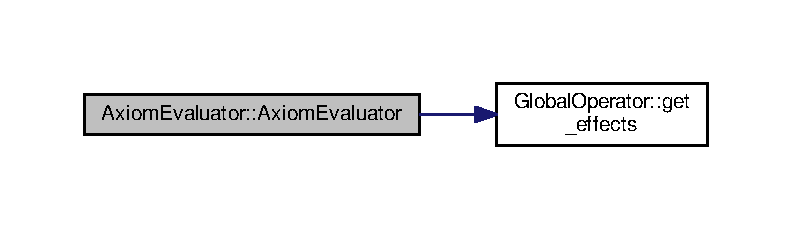
\includegraphics[width=350pt]{classAxiomEvaluator_a1ff4add414b7a5dcc6e2ca9bf71a5cc7_cgraph}
\end{center}
\end{figure}




\subsection{Member Function Documentation}
\hypertarget{classAxiomEvaluator_a470288573fe4c91aeedaa4b36dc7c4e1}{\index{Axiom\-Evaluator@{Axiom\-Evaluator}!evaluate@{evaluate}}
\index{evaluate@{evaluate}!AxiomEvaluator@{Axiom\-Evaluator}}
\subsubsection[{evaluate}]{\setlength{\rightskip}{0pt plus 5cm}void Axiom\-Evaluator\-::evaluate (
\begin{DoxyParamCaption}
\item[{{\bf Packed\-State\-Bin} $\ast$}]{buffer}
\end{DoxyParamCaption}
)}}\label{classAxiomEvaluator_a470288573fe4c91aeedaa4b36dc7c4e1}


Here is the call graph for this function\-:
\nopagebreak
\begin{figure}[H]
\begin{center}
\leavevmode
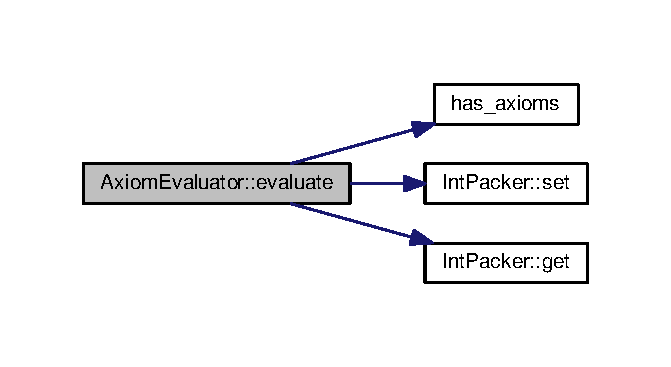
\includegraphics[width=322pt]{classAxiomEvaluator_a470288573fe4c91aeedaa4b36dc7c4e1_cgraph}
\end{center}
\end{figure}




The documentation for this class was generated from the following files\-:\begin{DoxyCompactItemize}
\item 
\hyperlink{axioms_8h}{axioms.\-h}\item 
\hyperlink{axioms_8cc}{axioms.\-cc}\end{DoxyCompactItemize}

\hypertarget{classAxiomsProxy}{\section{Axioms\-Proxy Class Reference}
\label{classAxiomsProxy}\index{Axioms\-Proxy@{Axioms\-Proxy}}
}


{\ttfamily \#include $<$task\-\_\-proxy.\-h$>$}

\subsection*{Public Types}
\begin{DoxyCompactItemize}
\item 
using \hyperlink{classAxiomsProxy_abefbb803d0603832ce3784793040cc30}{Item\-Type} = \hyperlink{classOperatorProxy}{Operator\-Proxy}
\end{DoxyCompactItemize}
\subsection*{Public Member Functions}
\begin{DoxyCompactItemize}
\item 
\hyperlink{classAxiomsProxy_aa06ac71778563a60523ec3e7fae56ef1}{Axioms\-Proxy} (const \hyperlink{classAbstractTask}{Abstract\-Task} \&task)
\item 
\hyperlink{classAxiomsProxy_a1f0a596925691361d514e875546dfebc}{$\sim$\-Axioms\-Proxy} ()=default
\item 
std\-::size\-\_\-t \hyperlink{classAxiomsProxy_aea7209589c94878185298ddf3a328720}{size} () const 
\item 
bool \hyperlink{classAxiomsProxy_ab246c21d3176f9c7f2d713a1d31c65dc}{empty} () const 
\item 
\hyperlink{classOperatorProxy}{Operator\-Proxy} \hyperlink{classAxiomsProxy_ab553b5ccabf34ab61180eb4f6ce80008}{operator\mbox{[}$\,$\mbox{]}} (std\-::size\-\_\-t index) const 
\end{DoxyCompactItemize}


\subsection{Member Typedef Documentation}
\hypertarget{classAxiomsProxy_abefbb803d0603832ce3784793040cc30}{\index{Axioms\-Proxy@{Axioms\-Proxy}!Item\-Type@{Item\-Type}}
\index{Item\-Type@{Item\-Type}!AxiomsProxy@{Axioms\-Proxy}}
\subsubsection[{Item\-Type}]{\setlength{\rightskip}{0pt plus 5cm}using {\bf Axioms\-Proxy\-::\-Item\-Type} =  {\bf Operator\-Proxy}}}\label{classAxiomsProxy_abefbb803d0603832ce3784793040cc30}


\subsection{Constructor \& Destructor Documentation}
\hypertarget{classAxiomsProxy_aa06ac71778563a60523ec3e7fae56ef1}{\index{Axioms\-Proxy@{Axioms\-Proxy}!Axioms\-Proxy@{Axioms\-Proxy}}
\index{Axioms\-Proxy@{Axioms\-Proxy}!AxiomsProxy@{Axioms\-Proxy}}
\subsubsection[{Axioms\-Proxy}]{\setlength{\rightskip}{0pt plus 5cm}Axioms\-Proxy\-::\-Axioms\-Proxy (
\begin{DoxyParamCaption}
\item[{const {\bf Abstract\-Task} \&}]{task}
\end{DoxyParamCaption}
)\hspace{0.3cm}{\ttfamily [inline]}, {\ttfamily [explicit]}}}\label{classAxiomsProxy_aa06ac71778563a60523ec3e7fae56ef1}
\hypertarget{classAxiomsProxy_a1f0a596925691361d514e875546dfebc}{\index{Axioms\-Proxy@{Axioms\-Proxy}!$\sim$\-Axioms\-Proxy@{$\sim$\-Axioms\-Proxy}}
\index{$\sim$\-Axioms\-Proxy@{$\sim$\-Axioms\-Proxy}!AxiomsProxy@{Axioms\-Proxy}}
\subsubsection[{$\sim$\-Axioms\-Proxy}]{\setlength{\rightskip}{0pt plus 5cm}Axioms\-Proxy\-::$\sim$\-Axioms\-Proxy (
\begin{DoxyParamCaption}
{}
\end{DoxyParamCaption}
)\hspace{0.3cm}{\ttfamily [default]}}}\label{classAxiomsProxy_a1f0a596925691361d514e875546dfebc}


\subsection{Member Function Documentation}
\hypertarget{classAxiomsProxy_ab246c21d3176f9c7f2d713a1d31c65dc}{\index{Axioms\-Proxy@{Axioms\-Proxy}!empty@{empty}}
\index{empty@{empty}!AxiomsProxy@{Axioms\-Proxy}}
\subsubsection[{empty}]{\setlength{\rightskip}{0pt plus 5cm}bool Axioms\-Proxy\-::empty (
\begin{DoxyParamCaption}
{}
\end{DoxyParamCaption}
) const\hspace{0.3cm}{\ttfamily [inline]}}}\label{classAxiomsProxy_ab246c21d3176f9c7f2d713a1d31c65dc}


Here is the call graph for this function\-:
\nopagebreak
\begin{figure}[H]
\begin{center}
\leavevmode
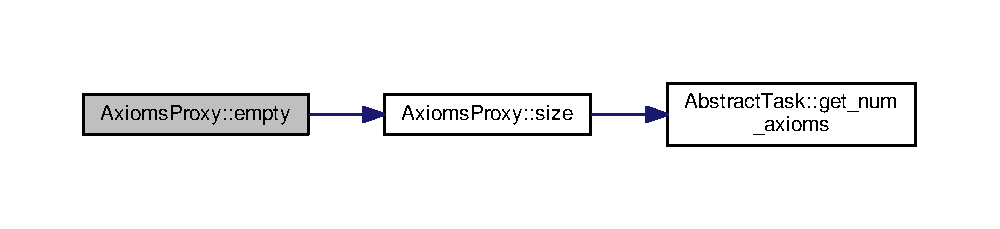
\includegraphics[width=350pt]{classAxiomsProxy_ab246c21d3176f9c7f2d713a1d31c65dc_cgraph}
\end{center}
\end{figure}


\hypertarget{classAxiomsProxy_ab553b5ccabf34ab61180eb4f6ce80008}{\index{Axioms\-Proxy@{Axioms\-Proxy}!operator\mbox{[}$\,$\mbox{]}@{operator[]}}
\index{operator\mbox{[}$\,$\mbox{]}@{operator[]}!AxiomsProxy@{Axioms\-Proxy}}
\subsubsection[{operator[]}]{\setlength{\rightskip}{0pt plus 5cm}{\bf Operator\-Proxy} Axioms\-Proxy\-::operator\mbox{[}$\,$\mbox{]} (
\begin{DoxyParamCaption}
\item[{std\-::size\-\_\-t}]{index}
\end{DoxyParamCaption}
) const\hspace{0.3cm}{\ttfamily [inline]}}}\label{classAxiomsProxy_ab553b5ccabf34ab61180eb4f6ce80008}


Here is the call graph for this function\-:
\nopagebreak
\begin{figure}[H]
\begin{center}
\leavevmode
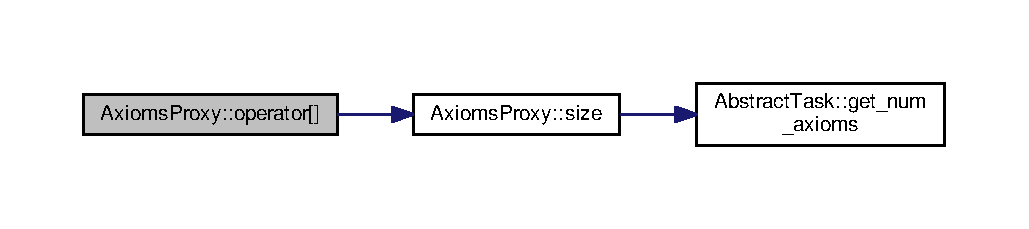
\includegraphics[width=350pt]{classAxiomsProxy_ab553b5ccabf34ab61180eb4f6ce80008_cgraph}
\end{center}
\end{figure}


\hypertarget{classAxiomsProxy_aea7209589c94878185298ddf3a328720}{\index{Axioms\-Proxy@{Axioms\-Proxy}!size@{size}}
\index{size@{size}!AxiomsProxy@{Axioms\-Proxy}}
\subsubsection[{size}]{\setlength{\rightskip}{0pt plus 5cm}std\-::size\-\_\-t Axioms\-Proxy\-::size (
\begin{DoxyParamCaption}
{}
\end{DoxyParamCaption}
) const\hspace{0.3cm}{\ttfamily [inline]}}}\label{classAxiomsProxy_aea7209589c94878185298ddf3a328720}


Here is the call graph for this function\-:
\nopagebreak
\begin{figure}[H]
\begin{center}
\leavevmode
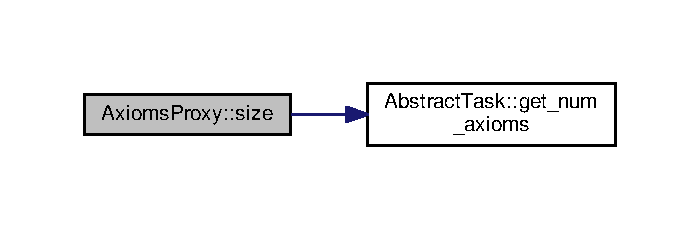
\includegraphics[width=336pt]{classAxiomsProxy_aea7209589c94878185298ddf3a328720_cgraph}
\end{center}
\end{figure}




The documentation for this class was generated from the following file\-:\begin{DoxyCompactItemize}
\item 
\hyperlink{task__proxy_8h}{task\-\_\-proxy.\-h}\end{DoxyCompactItemize}

\hypertarget{classBlindSearchHeuristic}{\section{Blind\-Search\-Heuristic Class Reference}
\label{classBlindSearchHeuristic}\index{Blind\-Search\-Heuristic@{Blind\-Search\-Heuristic}}
}


{\ttfamily \#include $<$blind\-\_\-search\-\_\-heuristic.\-h$>$}



Inheritance diagram for Blind\-Search\-Heuristic\-:
\nopagebreak
\begin{figure}[H]
\begin{center}
\leavevmode
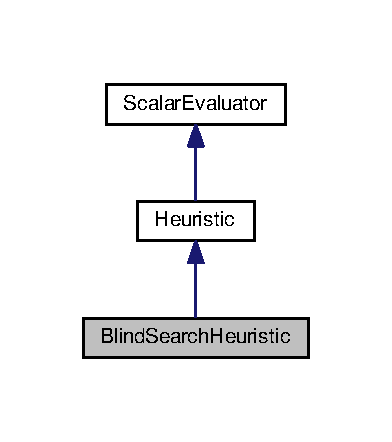
\includegraphics[width=188pt]{classBlindSearchHeuristic__inherit__graph}
\end{center}
\end{figure}


Collaboration diagram for Blind\-Search\-Heuristic\-:
\nopagebreak
\begin{figure}[H]
\begin{center}
\leavevmode
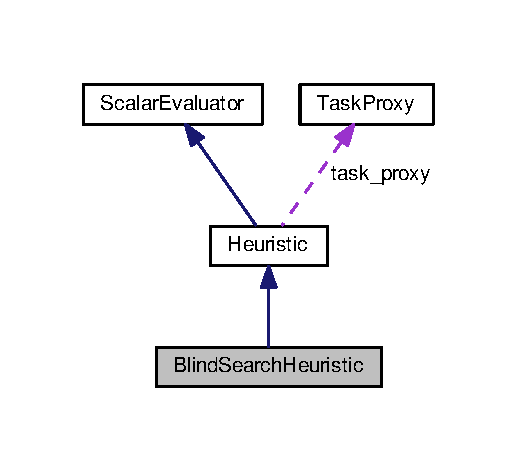
\includegraphics[width=248pt]{classBlindSearchHeuristic__coll__graph}
\end{center}
\end{figure}
\subsection*{Public Member Functions}
\begin{DoxyCompactItemize}
\item 
\hyperlink{classBlindSearchHeuristic_af684ed73096822d1d8e2d8fe27d7f974}{Blind\-Search\-Heuristic} (const \hyperlink{classOptions}{Options} \&options)
\item 
\hyperlink{classBlindSearchHeuristic_ab9526193265e07f7cfd96487ecada877}{$\sim$\-Blind\-Search\-Heuristic} ()
\end{DoxyCompactItemize}
\subsection*{Protected Member Functions}
\begin{DoxyCompactItemize}
\item 
virtual void \hyperlink{classBlindSearchHeuristic_af7490dcb3e01284dd673f35810983253}{initialize} ()
\item 
virtual int \hyperlink{classBlindSearchHeuristic_a7a6527bad7788c79a80811f6dacefa64}{compute\-\_\-heuristic} (const \hyperlink{classGlobalState}{Global\-State} \&global\-\_\-state)
\end{DoxyCompactItemize}
\subsection*{Additional Inherited Members}


\subsection{Constructor \& Destructor Documentation}
\hypertarget{classBlindSearchHeuristic_af684ed73096822d1d8e2d8fe27d7f974}{\index{Blind\-Search\-Heuristic@{Blind\-Search\-Heuristic}!Blind\-Search\-Heuristic@{Blind\-Search\-Heuristic}}
\index{Blind\-Search\-Heuristic@{Blind\-Search\-Heuristic}!BlindSearchHeuristic@{Blind\-Search\-Heuristic}}
\subsubsection[{Blind\-Search\-Heuristic}]{\setlength{\rightskip}{0pt plus 5cm}Blind\-Search\-Heuristic\-::\-Blind\-Search\-Heuristic (
\begin{DoxyParamCaption}
\item[{const {\bf Options} \&}]{options}
\end{DoxyParamCaption}
)}}\label{classBlindSearchHeuristic_af684ed73096822d1d8e2d8fe27d7f974}


Here is the call graph for this function\-:
\nopagebreak
\begin{figure}[H]
\begin{center}
\leavevmode
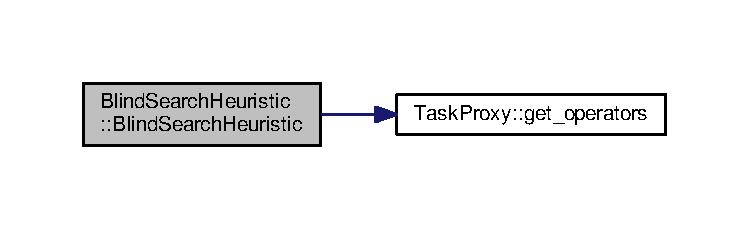
\includegraphics[width=350pt]{classBlindSearchHeuristic_af684ed73096822d1d8e2d8fe27d7f974_cgraph}
\end{center}
\end{figure}


\hypertarget{classBlindSearchHeuristic_ab9526193265e07f7cfd96487ecada877}{\index{Blind\-Search\-Heuristic@{Blind\-Search\-Heuristic}!$\sim$\-Blind\-Search\-Heuristic@{$\sim$\-Blind\-Search\-Heuristic}}
\index{$\sim$\-Blind\-Search\-Heuristic@{$\sim$\-Blind\-Search\-Heuristic}!BlindSearchHeuristic@{Blind\-Search\-Heuristic}}
\subsubsection[{$\sim$\-Blind\-Search\-Heuristic}]{\setlength{\rightskip}{0pt plus 5cm}Blind\-Search\-Heuristic\-::$\sim$\-Blind\-Search\-Heuristic (
\begin{DoxyParamCaption}
{}
\end{DoxyParamCaption}
)}}\label{classBlindSearchHeuristic_ab9526193265e07f7cfd96487ecada877}


\subsection{Member Function Documentation}
\hypertarget{classBlindSearchHeuristic_a7a6527bad7788c79a80811f6dacefa64}{\index{Blind\-Search\-Heuristic@{Blind\-Search\-Heuristic}!compute\-\_\-heuristic@{compute\-\_\-heuristic}}
\index{compute\-\_\-heuristic@{compute\-\_\-heuristic}!BlindSearchHeuristic@{Blind\-Search\-Heuristic}}
\subsubsection[{compute\-\_\-heuristic}]{\setlength{\rightskip}{0pt plus 5cm}int Blind\-Search\-Heuristic\-::compute\-\_\-heuristic (
\begin{DoxyParamCaption}
\item[{const {\bf Global\-State} \&}]{global\-\_\-state}
\end{DoxyParamCaption}
)\hspace{0.3cm}{\ttfamily [protected]}, {\ttfamily [virtual]}}}\label{classBlindSearchHeuristic_a7a6527bad7788c79a80811f6dacefa64}


Implements \hyperlink{classHeuristic_a4fd4e087281805e0e76a814e06d4e506}{Heuristic}.



Here is the call graph for this function\-:
\nopagebreak
\begin{figure}[H]
\begin{center}
\leavevmode
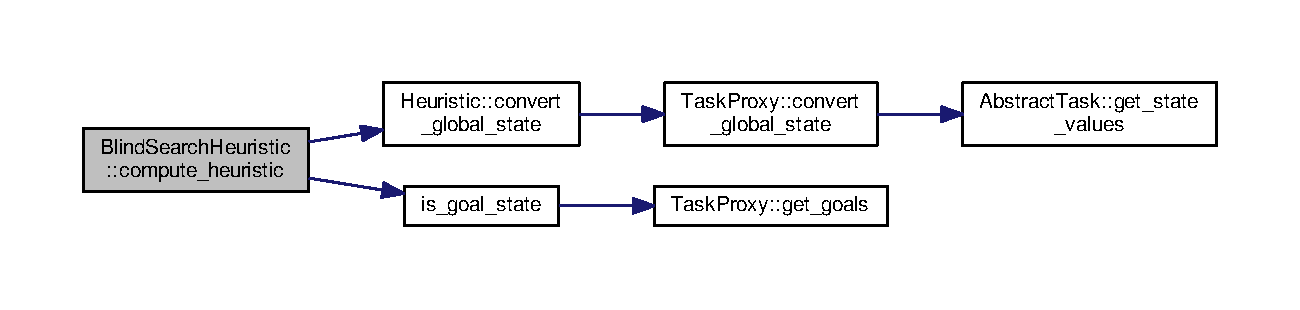
\includegraphics[width=350pt]{classBlindSearchHeuristic_a7a6527bad7788c79a80811f6dacefa64_cgraph}
\end{center}
\end{figure}


\hypertarget{classBlindSearchHeuristic_af7490dcb3e01284dd673f35810983253}{\index{Blind\-Search\-Heuristic@{Blind\-Search\-Heuristic}!initialize@{initialize}}
\index{initialize@{initialize}!BlindSearchHeuristic@{Blind\-Search\-Heuristic}}
\subsubsection[{initialize}]{\setlength{\rightskip}{0pt plus 5cm}void Blind\-Search\-Heuristic\-::initialize (
\begin{DoxyParamCaption}
{}
\end{DoxyParamCaption}
)\hspace{0.3cm}{\ttfamily [protected]}, {\ttfamily [virtual]}}}\label{classBlindSearchHeuristic_af7490dcb3e01284dd673f35810983253}


Reimplemented from \hyperlink{classHeuristic_a26e75bad1d806657c0ed274b4fe72f0a}{Heuristic}.



The documentation for this class was generated from the following files\-:\begin{DoxyCompactItemize}
\item 
\hyperlink{blind__search__heuristic_8h}{blind\-\_\-search\-\_\-heuristic.\-h}\item 
\hyperlink{blind__search__heuristic_8cc}{blind\-\_\-search\-\_\-heuristic.\-cc}\end{DoxyCompactItemize}

\hypertarget{classBlock}{\section{Block Class Reference}
\label{classBlock}\index{Block@{Block}}
}


{\ttfamily \#include $<$equivalence\-\_\-relation.\-h$>$}

\subsection*{Public Member Functions}
\begin{DoxyCompactItemize}
\item 
bool \hyperlink{classBlock_aa7bd121892cfaf6b809770743b722881}{empty} () const 
\item 
\hyperlink{equivalence__relation_8h_a22c88987f7fe558cb3981e02adfe10f9}{Element\-List\-Iter} \hyperlink{classBlock_a8dd3b62565b39719d5065bcb3a602a6f}{insert} (int element)
\item 
void \hyperlink{classBlock_a5bb954a6dd64cf7ab961eb3b73c7c526}{erase} (\hyperlink{equivalence__relation_8h_a22c88987f7fe558cb3981e02adfe10f9}{Element\-List\-Iter} it)
\item 
\hyperlink{equivalence__relation_8h_a22c88987f7fe558cb3981e02adfe10f9}{Element\-List\-Iter} \hyperlink{classBlock_acf6b48387e121c13be045cbdfa7b8728}{begin} ()
\item 
\hyperlink{equivalence__relation_8h_a22c88987f7fe558cb3981e02adfe10f9}{Element\-List\-Iter} \hyperlink{classBlock_a69a6fd777d86ac7538cd67972659428c}{end} ()
\item 
\hyperlink{equivalence__relation_8h_adcd1a68c6846e41421e3868fd40bdd81}{Element\-List\-Const\-Iter} \hyperlink{classBlock_ae4f1ad69095490a589c891c565f85ac4}{begin} () const 
\item 
\hyperlink{equivalence__relation_8h_adcd1a68c6846e41421e3868fd40bdd81}{Element\-List\-Const\-Iter} \hyperlink{classBlock_a836ea3d46f2fdc517124bdd742721fa5}{end} () const 
\end{DoxyCompactItemize}
\subsection*{Friends}
\begin{DoxyCompactItemize}
\item 
class \hyperlink{classBlock_a3075bd6f6bf3f78b0f8befb721ac3f61}{Equivalence\-Relation}
\end{DoxyCompactItemize}


\subsection{Member Function Documentation}
\hypertarget{classBlock_acf6b48387e121c13be045cbdfa7b8728}{\index{Block@{Block}!begin@{begin}}
\index{begin@{begin}!Block@{Block}}
\subsubsection[{begin}]{\setlength{\rightskip}{0pt plus 5cm}{\bf Element\-List\-Iter} Block\-::begin (
\begin{DoxyParamCaption}
{}
\end{DoxyParamCaption}
)\hspace{0.3cm}{\ttfamily [inline]}}}\label{classBlock_acf6b48387e121c13be045cbdfa7b8728}
\hypertarget{classBlock_ae4f1ad69095490a589c891c565f85ac4}{\index{Block@{Block}!begin@{begin}}
\index{begin@{begin}!Block@{Block}}
\subsubsection[{begin}]{\setlength{\rightskip}{0pt plus 5cm}{\bf Element\-List\-Const\-Iter} Block\-::begin (
\begin{DoxyParamCaption}
{}
\end{DoxyParamCaption}
) const\hspace{0.3cm}{\ttfamily [inline]}}}\label{classBlock_ae4f1ad69095490a589c891c565f85ac4}
\hypertarget{classBlock_aa7bd121892cfaf6b809770743b722881}{\index{Block@{Block}!empty@{empty}}
\index{empty@{empty}!Block@{Block}}
\subsubsection[{empty}]{\setlength{\rightskip}{0pt plus 5cm}bool Block\-::empty (
\begin{DoxyParamCaption}
{}
\end{DoxyParamCaption}
) const}}\label{classBlock_aa7bd121892cfaf6b809770743b722881}
\hypertarget{classBlock_a69a6fd777d86ac7538cd67972659428c}{\index{Block@{Block}!end@{end}}
\index{end@{end}!Block@{Block}}
\subsubsection[{end}]{\setlength{\rightskip}{0pt plus 5cm}{\bf Element\-List\-Iter} Block\-::end (
\begin{DoxyParamCaption}
{}
\end{DoxyParamCaption}
)\hspace{0.3cm}{\ttfamily [inline]}}}\label{classBlock_a69a6fd777d86ac7538cd67972659428c}
\hypertarget{classBlock_a836ea3d46f2fdc517124bdd742721fa5}{\index{Block@{Block}!end@{end}}
\index{end@{end}!Block@{Block}}
\subsubsection[{end}]{\setlength{\rightskip}{0pt plus 5cm}{\bf Element\-List\-Const\-Iter} Block\-::end (
\begin{DoxyParamCaption}
{}
\end{DoxyParamCaption}
) const\hspace{0.3cm}{\ttfamily [inline]}}}\label{classBlock_a836ea3d46f2fdc517124bdd742721fa5}
\hypertarget{classBlock_a5bb954a6dd64cf7ab961eb3b73c7c526}{\index{Block@{Block}!erase@{erase}}
\index{erase@{erase}!Block@{Block}}
\subsubsection[{erase}]{\setlength{\rightskip}{0pt plus 5cm}void Block\-::erase (
\begin{DoxyParamCaption}
\item[{{\bf Element\-List\-Iter}}]{it}
\end{DoxyParamCaption}
)}}\label{classBlock_a5bb954a6dd64cf7ab961eb3b73c7c526}
\hypertarget{classBlock_a8dd3b62565b39719d5065bcb3a602a6f}{\index{Block@{Block}!insert@{insert}}
\index{insert@{insert}!Block@{Block}}
\subsubsection[{insert}]{\setlength{\rightskip}{0pt plus 5cm}{\bf Element\-List\-Iter} Block\-::insert (
\begin{DoxyParamCaption}
\item[{int}]{element}
\end{DoxyParamCaption}
)}}\label{classBlock_a8dd3b62565b39719d5065bcb3a602a6f}


\subsection{Friends And Related Function Documentation}
\hypertarget{classBlock_a3075bd6f6bf3f78b0f8befb721ac3f61}{\index{Block@{Block}!Equivalence\-Relation@{Equivalence\-Relation}}
\index{Equivalence\-Relation@{Equivalence\-Relation}!Block@{Block}}
\subsubsection[{Equivalence\-Relation}]{\setlength{\rightskip}{0pt plus 5cm}friend class {\bf Equivalence\-Relation}\hspace{0.3cm}{\ttfamily [friend]}}}\label{classBlock_a3075bd6f6bf3f78b0f8befb721ac3f61}


The documentation for this class was generated from the following files\-:\begin{DoxyCompactItemize}
\item 
\hyperlink{equivalence__relation_8h}{equivalence\-\_\-relation.\-h}\item 
\hyperlink{equivalence__relation_8cc}{equivalence\-\_\-relation.\-cc}\end{DoxyCompactItemize}

\hypertarget{classBucketQueue}{\section{Bucket\-Queue$<$ Value $>$ Class Template Reference}
\label{classBucketQueue}\index{Bucket\-Queue$<$ Value $>$@{Bucket\-Queue$<$ Value $>$}}
}


{\ttfamily \#include $<$priority\-\_\-queue.\-h$>$}



Inheritance diagram for Bucket\-Queue$<$ Value $>$\-:
\nopagebreak
\begin{figure}[H]
\begin{center}
\leavevmode
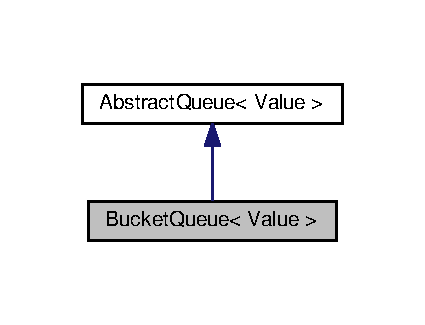
\includegraphics[width=204pt]{classBucketQueue__inherit__graph}
\end{center}
\end{figure}


Collaboration diagram for Bucket\-Queue$<$ Value $>$\-:
\nopagebreak
\begin{figure}[H]
\begin{center}
\leavevmode
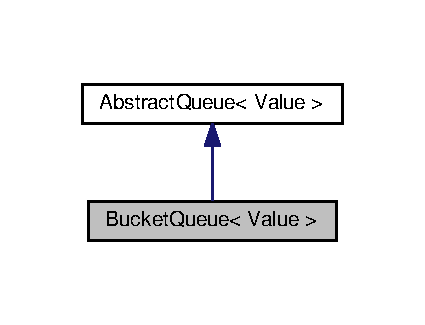
\includegraphics[width=204pt]{classBucketQueue__coll__graph}
\end{center}
\end{figure}
\subsection*{Public Member Functions}
\begin{DoxyCompactItemize}
\item 
\hyperlink{classBucketQueue_a160b83709a877ee92251c3667fa5d108}{Bucket\-Queue} ()
\item 
virtual \hyperlink{classBucketQueue_aa9afef340657720fda376238977180e5}{$\sim$\-Bucket\-Queue} ()
\item 
virtual void \hyperlink{classBucketQueue_a1dc89d8bd4fd657dfc0218ca947f0d24}{push} (int key, const Value \&value)
\item 
virtual \hyperlink{classAbstractQueue_abe60381528bc4cf9d4032f33f2ff6f3c}{Entry} \hyperlink{classBucketQueue_a2141b91ece1d2180d56ec74f07aa747e}{pop} ()
\item 
virtual bool \hyperlink{classBucketQueue_a3cf60e426df86413789dc19beee350b3}{empty} () const 
\item 
virtual void \hyperlink{classBucketQueue_a749f5dc24bb6bb5754cb78f677b97d26}{clear} ()
\item 
virtual \hyperlink{classAbstractQueue}{Abstract\-Queue}$<$ Value $>$ $\ast$ \hyperlink{classBucketQueue_a4d56a716545e8a2a6e11481cd07d01ac}{convert\-\_\-if\-\_\-necessary} (int key)
\item 
virtual void \hyperlink{classBucketQueue_a362473bbbcf135376ec07be1b651b49d}{add\-\_\-virtual\-\_\-pushes} (int num\-\_\-extra\-\_\-pushes)
\end{DoxyCompactItemize}
\subsection*{Additional Inherited Members}


\subsection{Constructor \& Destructor Documentation}
\hypertarget{classBucketQueue_a160b83709a877ee92251c3667fa5d108}{\index{Bucket\-Queue@{Bucket\-Queue}!Bucket\-Queue@{Bucket\-Queue}}
\index{Bucket\-Queue@{Bucket\-Queue}!BucketQueue@{Bucket\-Queue}}
\subsubsection[{Bucket\-Queue}]{\setlength{\rightskip}{0pt plus 5cm}template$<$typename Value $>$ {\bf Bucket\-Queue}$<$ Value $>$\-::{\bf Bucket\-Queue} (
\begin{DoxyParamCaption}
{}
\end{DoxyParamCaption}
)\hspace{0.3cm}{\ttfamily [inline]}}}\label{classBucketQueue_a160b83709a877ee92251c3667fa5d108}
\hypertarget{classBucketQueue_aa9afef340657720fda376238977180e5}{\index{Bucket\-Queue@{Bucket\-Queue}!$\sim$\-Bucket\-Queue@{$\sim$\-Bucket\-Queue}}
\index{$\sim$\-Bucket\-Queue@{$\sim$\-Bucket\-Queue}!BucketQueue@{Bucket\-Queue}}
\subsubsection[{$\sim$\-Bucket\-Queue}]{\setlength{\rightskip}{0pt plus 5cm}template$<$typename Value $>$ virtual {\bf Bucket\-Queue}$<$ Value $>$\-::$\sim${\bf Bucket\-Queue} (
\begin{DoxyParamCaption}
{}
\end{DoxyParamCaption}
)\hspace{0.3cm}{\ttfamily [inline]}, {\ttfamily [virtual]}}}\label{classBucketQueue_aa9afef340657720fda376238977180e5}


\subsection{Member Function Documentation}
\hypertarget{classBucketQueue_a362473bbbcf135376ec07be1b651b49d}{\index{Bucket\-Queue@{Bucket\-Queue}!add\-\_\-virtual\-\_\-pushes@{add\-\_\-virtual\-\_\-pushes}}
\index{add\-\_\-virtual\-\_\-pushes@{add\-\_\-virtual\-\_\-pushes}!BucketQueue@{Bucket\-Queue}}
\subsubsection[{add\-\_\-virtual\-\_\-pushes}]{\setlength{\rightskip}{0pt plus 5cm}template$<$typename Value $>$ virtual void {\bf Bucket\-Queue}$<$ Value $>$\-::add\-\_\-virtual\-\_\-pushes (
\begin{DoxyParamCaption}
\item[{int}]{num\-\_\-extra\-\_\-pushes}
\end{DoxyParamCaption}
)\hspace{0.3cm}{\ttfamily [inline]}, {\ttfamily [virtual]}}}\label{classBucketQueue_a362473bbbcf135376ec07be1b651b49d}


Implements \hyperlink{classAbstractQueue_a2db622c67d66a0ee3d18e9e98145ece9}{Abstract\-Queue$<$ Value $>$}.

\hypertarget{classBucketQueue_a749f5dc24bb6bb5754cb78f677b97d26}{\index{Bucket\-Queue@{Bucket\-Queue}!clear@{clear}}
\index{clear@{clear}!BucketQueue@{Bucket\-Queue}}
\subsubsection[{clear}]{\setlength{\rightskip}{0pt plus 5cm}template$<$typename Value $>$ virtual void {\bf Bucket\-Queue}$<$ Value $>$\-::clear (
\begin{DoxyParamCaption}
{}
\end{DoxyParamCaption}
)\hspace{0.3cm}{\ttfamily [inline]}, {\ttfamily [virtual]}}}\label{classBucketQueue_a749f5dc24bb6bb5754cb78f677b97d26}


Implements \hyperlink{classAbstractQueue_a2e976dcbc1ca3e97d05591cd466ff3e7}{Abstract\-Queue$<$ Value $>$}.



Here is the call graph for this function\-:
\nopagebreak
\begin{figure}[H]
\begin{center}
\leavevmode
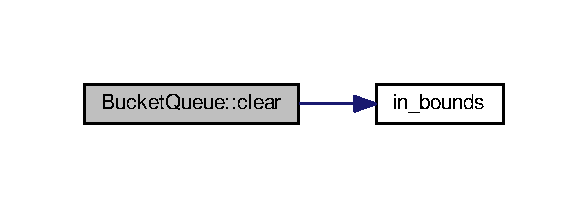
\includegraphics[width=282pt]{classBucketQueue_a749f5dc24bb6bb5754cb78f677b97d26_cgraph}
\end{center}
\end{figure}


\hypertarget{classBucketQueue_a4d56a716545e8a2a6e11481cd07d01ac}{\index{Bucket\-Queue@{Bucket\-Queue}!convert\-\_\-if\-\_\-necessary@{convert\-\_\-if\-\_\-necessary}}
\index{convert\-\_\-if\-\_\-necessary@{convert\-\_\-if\-\_\-necessary}!BucketQueue@{Bucket\-Queue}}
\subsubsection[{convert\-\_\-if\-\_\-necessary}]{\setlength{\rightskip}{0pt plus 5cm}template$<$typename Value $>$ virtual {\bf Abstract\-Queue}$<$Value$>$$\ast$ {\bf Bucket\-Queue}$<$ Value $>$\-::convert\-\_\-if\-\_\-necessary (
\begin{DoxyParamCaption}
\item[{int}]{key}
\end{DoxyParamCaption}
)\hspace{0.3cm}{\ttfamily [inline]}, {\ttfamily [virtual]}}}\label{classBucketQueue_a4d56a716545e8a2a6e11481cd07d01ac}


Reimplemented from \hyperlink{classAbstractQueue_a4c9793d6ec0442bbf806c2f57d6fd426}{Abstract\-Queue$<$ Value $>$}.



Here is the call graph for this function\-:
\nopagebreak
\begin{figure}[H]
\begin{center}
\leavevmode
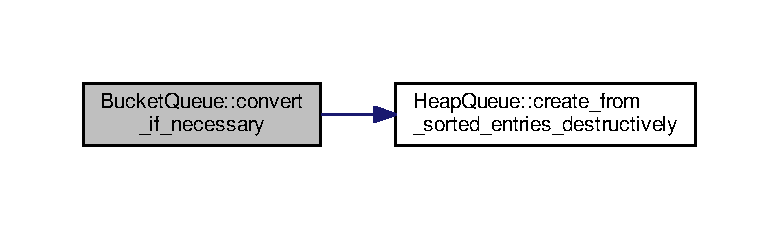
\includegraphics[width=350pt]{classBucketQueue_a4d56a716545e8a2a6e11481cd07d01ac_cgraph}
\end{center}
\end{figure}


\hypertarget{classBucketQueue_a3cf60e426df86413789dc19beee350b3}{\index{Bucket\-Queue@{Bucket\-Queue}!empty@{empty}}
\index{empty@{empty}!BucketQueue@{Bucket\-Queue}}
\subsubsection[{empty}]{\setlength{\rightskip}{0pt plus 5cm}template$<$typename Value $>$ virtual bool {\bf Bucket\-Queue}$<$ Value $>$\-::empty (
\begin{DoxyParamCaption}
{}
\end{DoxyParamCaption}
) const\hspace{0.3cm}{\ttfamily [inline]}, {\ttfamily [virtual]}}}\label{classBucketQueue_a3cf60e426df86413789dc19beee350b3}


Implements \hyperlink{classAbstractQueue_a38635110a147c0c1914e0f2f277a10de}{Abstract\-Queue$<$ Value $>$}.

\hypertarget{classBucketQueue_a2141b91ece1d2180d56ec74f07aa747e}{\index{Bucket\-Queue@{Bucket\-Queue}!pop@{pop}}
\index{pop@{pop}!BucketQueue@{Bucket\-Queue}}
\subsubsection[{pop}]{\setlength{\rightskip}{0pt plus 5cm}template$<$typename Value $>$ virtual {\bf Entry} {\bf Bucket\-Queue}$<$ Value $>$\-::pop (
\begin{DoxyParamCaption}
{}
\end{DoxyParamCaption}
)\hspace{0.3cm}{\ttfamily [inline]}, {\ttfamily [virtual]}}}\label{classBucketQueue_a2141b91ece1d2180d56ec74f07aa747e}


Implements \hyperlink{classAbstractQueue_aaec692216c729a7e7ca79b02a826cbf3}{Abstract\-Queue$<$ Value $>$}.

\hypertarget{classBucketQueue_a1dc89d8bd4fd657dfc0218ca947f0d24}{\index{Bucket\-Queue@{Bucket\-Queue}!push@{push}}
\index{push@{push}!BucketQueue@{Bucket\-Queue}}
\subsubsection[{push}]{\setlength{\rightskip}{0pt plus 5cm}template$<$typename Value $>$ virtual void {\bf Bucket\-Queue}$<$ Value $>$\-::push (
\begin{DoxyParamCaption}
\item[{int}]{key, }
\item[{const Value \&}]{value}
\end{DoxyParamCaption}
)\hspace{0.3cm}{\ttfamily [inline]}, {\ttfamily [virtual]}}}\label{classBucketQueue_a1dc89d8bd4fd657dfc0218ca947f0d24}


Implements \hyperlink{classAbstractQueue_af9268b0501749d8ab1b220a5db62a24e}{Abstract\-Queue$<$ Value $>$}.



The documentation for this class was generated from the following file\-:\begin{DoxyCompactItemize}
\item 
\hyperlink{priority__queue_8h}{priority\-\_\-queue.\-h}\end{DoxyCompactItemize}

\hypertarget{classCausalGraph}{\section{Causal\-Graph Class Reference}
\label{classCausalGraph}\index{Causal\-Graph@{Causal\-Graph}}
}


{\ttfamily \#include $<$causal\-\_\-graph.\-h$>$}

\subsection*{Public Member Functions}
\begin{DoxyCompactItemize}
\item 
\hyperlink{classCausalGraph_a98f5dcff9e838b52ce3a0c1ab3cd97e1}{Causal\-Graph} (const \hyperlink{classTaskProxy}{Task\-Proxy} \&task\-\_\-proxy)
\item 
\hyperlink{classCausalGraph_a9d61e3e1d4a35f4a4357a73ced3bc103}{$\sim$\-Causal\-Graph} ()=default
\item 
const std\-::vector$<$ int $>$ \& \hyperlink{classCausalGraph_a8ca093f0188ed6e141d8eaae0ada5130}{get\-\_\-pre\-\_\-to\-\_\-eff} (int var) const 
\item 
const std\-::vector$<$ int $>$ \& \hyperlink{classCausalGraph_a7d2ce555c4acdd613be7c20a4d1feec2}{get\-\_\-eff\-\_\-to\-\_\-pre} (int var) const 
\item 
const std\-::vector$<$ int $>$ \& \hyperlink{classCausalGraph_a28bbafcf1a02d63a037c5bb5d439c6fb}{get\-\_\-eff\-\_\-to\-\_\-eff} (int var) const 
\item 
const std\-::vector$<$ int $>$ \& \hyperlink{classCausalGraph_a4f949e7f3ca175ff25a5dd24bcee9dd0}{get\-\_\-successors} (int var) const 
\item 
const std\-::vector$<$ int $>$ \& \hyperlink{classCausalGraph_a21c18f6f34874deae1a493fd963271a8}{get\-\_\-predecessors} (int var) const 
\end{DoxyCompactItemize}


\subsection{Constructor \& Destructor Documentation}
\hypertarget{classCausalGraph_a98f5dcff9e838b52ce3a0c1ab3cd97e1}{\index{Causal\-Graph@{Causal\-Graph}!Causal\-Graph@{Causal\-Graph}}
\index{Causal\-Graph@{Causal\-Graph}!CausalGraph@{Causal\-Graph}}
\subsubsection[{Causal\-Graph}]{\setlength{\rightskip}{0pt plus 5cm}Causal\-Graph\-::\-Causal\-Graph (
\begin{DoxyParamCaption}
\item[{const {\bf Task\-Proxy} \&}]{task\-\_\-proxy}
\end{DoxyParamCaption}
)\hspace{0.3cm}{\ttfamily [explicit]}}}\label{classCausalGraph_a98f5dcff9e838b52ce3a0c1ab3cd97e1}


Here is the call graph for this function\-:
\nopagebreak
\begin{figure}[H]
\begin{center}
\leavevmode
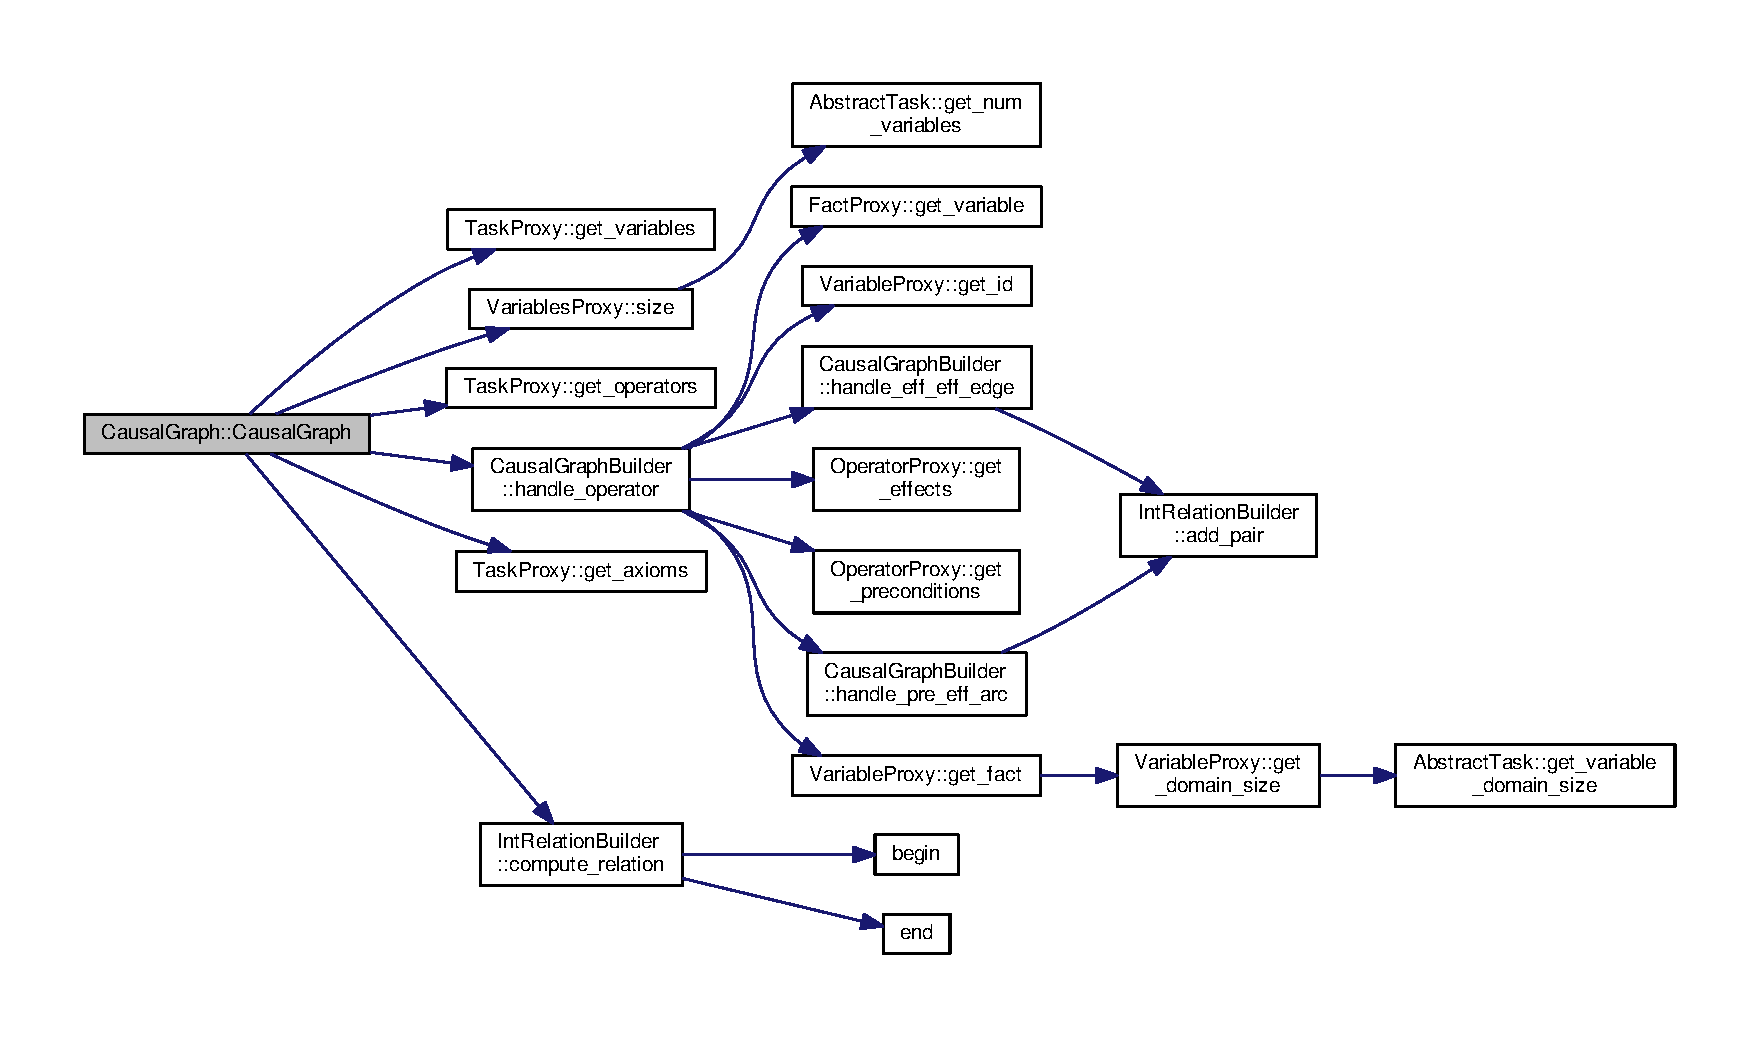
\includegraphics[width=350pt]{classCausalGraph_a98f5dcff9e838b52ce3a0c1ab3cd97e1_cgraph}
\end{center}
\end{figure}


\hypertarget{classCausalGraph_a9d61e3e1d4a35f4a4357a73ced3bc103}{\index{Causal\-Graph@{Causal\-Graph}!$\sim$\-Causal\-Graph@{$\sim$\-Causal\-Graph}}
\index{$\sim$\-Causal\-Graph@{$\sim$\-Causal\-Graph}!CausalGraph@{Causal\-Graph}}
\subsubsection[{$\sim$\-Causal\-Graph}]{\setlength{\rightskip}{0pt plus 5cm}Causal\-Graph\-::$\sim$\-Causal\-Graph (
\begin{DoxyParamCaption}
{}
\end{DoxyParamCaption}
)\hspace{0.3cm}{\ttfamily [default]}}}\label{classCausalGraph_a9d61e3e1d4a35f4a4357a73ced3bc103}


\subsection{Member Function Documentation}
\hypertarget{classCausalGraph_a28bbafcf1a02d63a037c5bb5d439c6fb}{\index{Causal\-Graph@{Causal\-Graph}!get\-\_\-eff\-\_\-to\-\_\-eff@{get\-\_\-eff\-\_\-to\-\_\-eff}}
\index{get\-\_\-eff\-\_\-to\-\_\-eff@{get\-\_\-eff\-\_\-to\-\_\-eff}!CausalGraph@{Causal\-Graph}}
\subsubsection[{get\-\_\-eff\-\_\-to\-\_\-eff}]{\setlength{\rightskip}{0pt plus 5cm}const std\-::vector$<$int$>$\& Causal\-Graph\-::get\-\_\-eff\-\_\-to\-\_\-eff (
\begin{DoxyParamCaption}
\item[{int}]{var}
\end{DoxyParamCaption}
) const\hspace{0.3cm}{\ttfamily [inline]}}}\label{classCausalGraph_a28bbafcf1a02d63a037c5bb5d439c6fb}
\hypertarget{classCausalGraph_a7d2ce555c4acdd613be7c20a4d1feec2}{\index{Causal\-Graph@{Causal\-Graph}!get\-\_\-eff\-\_\-to\-\_\-pre@{get\-\_\-eff\-\_\-to\-\_\-pre}}
\index{get\-\_\-eff\-\_\-to\-\_\-pre@{get\-\_\-eff\-\_\-to\-\_\-pre}!CausalGraph@{Causal\-Graph}}
\subsubsection[{get\-\_\-eff\-\_\-to\-\_\-pre}]{\setlength{\rightskip}{0pt plus 5cm}const std\-::vector$<$int$>$\& Causal\-Graph\-::get\-\_\-eff\-\_\-to\-\_\-pre (
\begin{DoxyParamCaption}
\item[{int}]{var}
\end{DoxyParamCaption}
) const\hspace{0.3cm}{\ttfamily [inline]}}}\label{classCausalGraph_a7d2ce555c4acdd613be7c20a4d1feec2}
\hypertarget{classCausalGraph_a8ca093f0188ed6e141d8eaae0ada5130}{\index{Causal\-Graph@{Causal\-Graph}!get\-\_\-pre\-\_\-to\-\_\-eff@{get\-\_\-pre\-\_\-to\-\_\-eff}}
\index{get\-\_\-pre\-\_\-to\-\_\-eff@{get\-\_\-pre\-\_\-to\-\_\-eff}!CausalGraph@{Causal\-Graph}}
\subsubsection[{get\-\_\-pre\-\_\-to\-\_\-eff}]{\setlength{\rightskip}{0pt plus 5cm}const std\-::vector$<$int$>$\& Causal\-Graph\-::get\-\_\-pre\-\_\-to\-\_\-eff (
\begin{DoxyParamCaption}
\item[{int}]{var}
\end{DoxyParamCaption}
) const\hspace{0.3cm}{\ttfamily [inline]}}}\label{classCausalGraph_a8ca093f0188ed6e141d8eaae0ada5130}
\hypertarget{classCausalGraph_a21c18f6f34874deae1a493fd963271a8}{\index{Causal\-Graph@{Causal\-Graph}!get\-\_\-predecessors@{get\-\_\-predecessors}}
\index{get\-\_\-predecessors@{get\-\_\-predecessors}!CausalGraph@{Causal\-Graph}}
\subsubsection[{get\-\_\-predecessors}]{\setlength{\rightskip}{0pt plus 5cm}const std\-::vector$<$int$>$\& Causal\-Graph\-::get\-\_\-predecessors (
\begin{DoxyParamCaption}
\item[{int}]{var}
\end{DoxyParamCaption}
) const\hspace{0.3cm}{\ttfamily [inline]}}}\label{classCausalGraph_a21c18f6f34874deae1a493fd963271a8}
\hypertarget{classCausalGraph_a4f949e7f3ca175ff25a5dd24bcee9dd0}{\index{Causal\-Graph@{Causal\-Graph}!get\-\_\-successors@{get\-\_\-successors}}
\index{get\-\_\-successors@{get\-\_\-successors}!CausalGraph@{Causal\-Graph}}
\subsubsection[{get\-\_\-successors}]{\setlength{\rightskip}{0pt plus 5cm}const std\-::vector$<$int$>$\& Causal\-Graph\-::get\-\_\-successors (
\begin{DoxyParamCaption}
\item[{int}]{var}
\end{DoxyParamCaption}
) const\hspace{0.3cm}{\ttfamily [inline]}}}\label{classCausalGraph_a4f949e7f3ca175ff25a5dd24bcee9dd0}


The documentation for this class was generated from the following files\-:\begin{DoxyCompactItemize}
\item 
\hyperlink{causal__graph_8h}{causal\-\_\-graph.\-h}\item 
\hyperlink{causal__graph_8cc}{causal\-\_\-graph.\-cc}\end{DoxyCompactItemize}

\hypertarget{structCausalGraphBuilder}{\section{Causal\-Graph\-Builder Struct Reference}
\label{structCausalGraphBuilder}\index{Causal\-Graph\-Builder@{Causal\-Graph\-Builder}}
}


Collaboration diagram for Causal\-Graph\-Builder\-:
\nopagebreak
\begin{figure}[H]
\begin{center}
\leavevmode
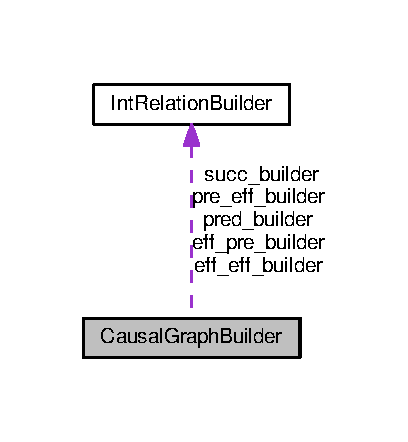
\includegraphics[width=196pt]{structCausalGraphBuilder__coll__graph}
\end{center}
\end{figure}
\subsection*{Public Member Functions}
\begin{DoxyCompactItemize}
\item 
\hyperlink{structCausalGraphBuilder_a220860e8bf4573f37608dc27ceae8a39}{Causal\-Graph\-Builder} (int var\-\_\-count)
\item 
\hyperlink{structCausalGraphBuilder_a2c87ca62dad3d471f4c9c16c122252ab}{$\sim$\-Causal\-Graph\-Builder} ()
\item 
void \hyperlink{structCausalGraphBuilder_a07d4a8c5185dd840b766f10b4927c858}{handle\-\_\-pre\-\_\-eff\-\_\-arc} (int u, int v)
\item 
void \hyperlink{structCausalGraphBuilder_a91630fdfada365f3e7274c3c70117ca9}{handle\-\_\-eff\-\_\-eff\-\_\-edge} (int u, int v)
\item 
void \hyperlink{structCausalGraphBuilder_adae0f168f463cd392b11b93430e5c7f9}{handle\-\_\-operator} (const \hyperlink{classOperatorProxy}{Operator\-Proxy} \&op)
\end{DoxyCompactItemize}
\subsection*{Public Attributes}
\begin{DoxyCompactItemize}
\item 
\hyperlink{classIntRelationBuilder}{Int\-Relation\-Builder} \hyperlink{structCausalGraphBuilder_a87a37c506c86e0e1332638066ac516e9}{pre\-\_\-eff\-\_\-builder}
\item 
\hyperlink{classIntRelationBuilder}{Int\-Relation\-Builder} \hyperlink{structCausalGraphBuilder_a773e4b6bc40fc74653a9d695f9983892}{eff\-\_\-pre\-\_\-builder}
\item 
\hyperlink{classIntRelationBuilder}{Int\-Relation\-Builder} \hyperlink{structCausalGraphBuilder_a3320af04c6485bdbf93345cf2e9cfeb1}{eff\-\_\-eff\-\_\-builder}
\item 
\hyperlink{classIntRelationBuilder}{Int\-Relation\-Builder} \hyperlink{structCausalGraphBuilder_a9a722f3782f6737608fd4b5fc8d9ea4e}{succ\-\_\-builder}
\item 
\hyperlink{classIntRelationBuilder}{Int\-Relation\-Builder} \hyperlink{structCausalGraphBuilder_a916b1495bcd680ca74c216e49187fede}{pred\-\_\-builder}
\end{DoxyCompactItemize}


\subsection{Constructor \& Destructor Documentation}
\hypertarget{structCausalGraphBuilder_a220860e8bf4573f37608dc27ceae8a39}{\index{Causal\-Graph\-Builder@{Causal\-Graph\-Builder}!Causal\-Graph\-Builder@{Causal\-Graph\-Builder}}
\index{Causal\-Graph\-Builder@{Causal\-Graph\-Builder}!CausalGraphBuilder@{Causal\-Graph\-Builder}}
\subsubsection[{Causal\-Graph\-Builder}]{\setlength{\rightskip}{0pt plus 5cm}Causal\-Graph\-Builder\-::\-Causal\-Graph\-Builder (
\begin{DoxyParamCaption}
\item[{int}]{var\-\_\-count}
\end{DoxyParamCaption}
)\hspace{0.3cm}{\ttfamily [inline]}, {\ttfamily [explicit]}}}\label{structCausalGraphBuilder_a220860e8bf4573f37608dc27ceae8a39}
\hypertarget{structCausalGraphBuilder_a2c87ca62dad3d471f4c9c16c122252ab}{\index{Causal\-Graph\-Builder@{Causal\-Graph\-Builder}!$\sim$\-Causal\-Graph\-Builder@{$\sim$\-Causal\-Graph\-Builder}}
\index{$\sim$\-Causal\-Graph\-Builder@{$\sim$\-Causal\-Graph\-Builder}!CausalGraphBuilder@{Causal\-Graph\-Builder}}
\subsubsection[{$\sim$\-Causal\-Graph\-Builder}]{\setlength{\rightskip}{0pt plus 5cm}Causal\-Graph\-Builder\-::$\sim$\-Causal\-Graph\-Builder (
\begin{DoxyParamCaption}
{}
\end{DoxyParamCaption}
)\hspace{0.3cm}{\ttfamily [inline]}}}\label{structCausalGraphBuilder_a2c87ca62dad3d471f4c9c16c122252ab}


\subsection{Member Function Documentation}
\hypertarget{structCausalGraphBuilder_a91630fdfada365f3e7274c3c70117ca9}{\index{Causal\-Graph\-Builder@{Causal\-Graph\-Builder}!handle\-\_\-eff\-\_\-eff\-\_\-edge@{handle\-\_\-eff\-\_\-eff\-\_\-edge}}
\index{handle\-\_\-eff\-\_\-eff\-\_\-edge@{handle\-\_\-eff\-\_\-eff\-\_\-edge}!CausalGraphBuilder@{Causal\-Graph\-Builder}}
\subsubsection[{handle\-\_\-eff\-\_\-eff\-\_\-edge}]{\setlength{\rightskip}{0pt plus 5cm}void Causal\-Graph\-Builder\-::handle\-\_\-eff\-\_\-eff\-\_\-edge (
\begin{DoxyParamCaption}
\item[{int}]{u, }
\item[{int}]{v}
\end{DoxyParamCaption}
)\hspace{0.3cm}{\ttfamily [inline]}}}\label{structCausalGraphBuilder_a91630fdfada365f3e7274c3c70117ca9}


Here is the call graph for this function\-:
\nopagebreak
\begin{figure}[H]
\begin{center}
\leavevmode
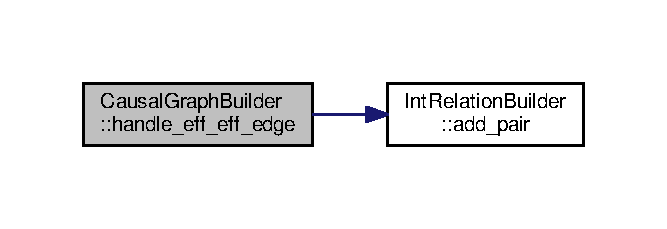
\includegraphics[width=320pt]{structCausalGraphBuilder_a91630fdfada365f3e7274c3c70117ca9_cgraph}
\end{center}
\end{figure}


\hypertarget{structCausalGraphBuilder_adae0f168f463cd392b11b93430e5c7f9}{\index{Causal\-Graph\-Builder@{Causal\-Graph\-Builder}!handle\-\_\-operator@{handle\-\_\-operator}}
\index{handle\-\_\-operator@{handle\-\_\-operator}!CausalGraphBuilder@{Causal\-Graph\-Builder}}
\subsubsection[{handle\-\_\-operator}]{\setlength{\rightskip}{0pt plus 5cm}void Causal\-Graph\-Builder\-::handle\-\_\-operator (
\begin{DoxyParamCaption}
\item[{const {\bf Operator\-Proxy} \&}]{op}
\end{DoxyParamCaption}
)\hspace{0.3cm}{\ttfamily [inline]}}}\label{structCausalGraphBuilder_adae0f168f463cd392b11b93430e5c7f9}


Here is the call graph for this function\-:
\nopagebreak
\begin{figure}[H]
\begin{center}
\leavevmode
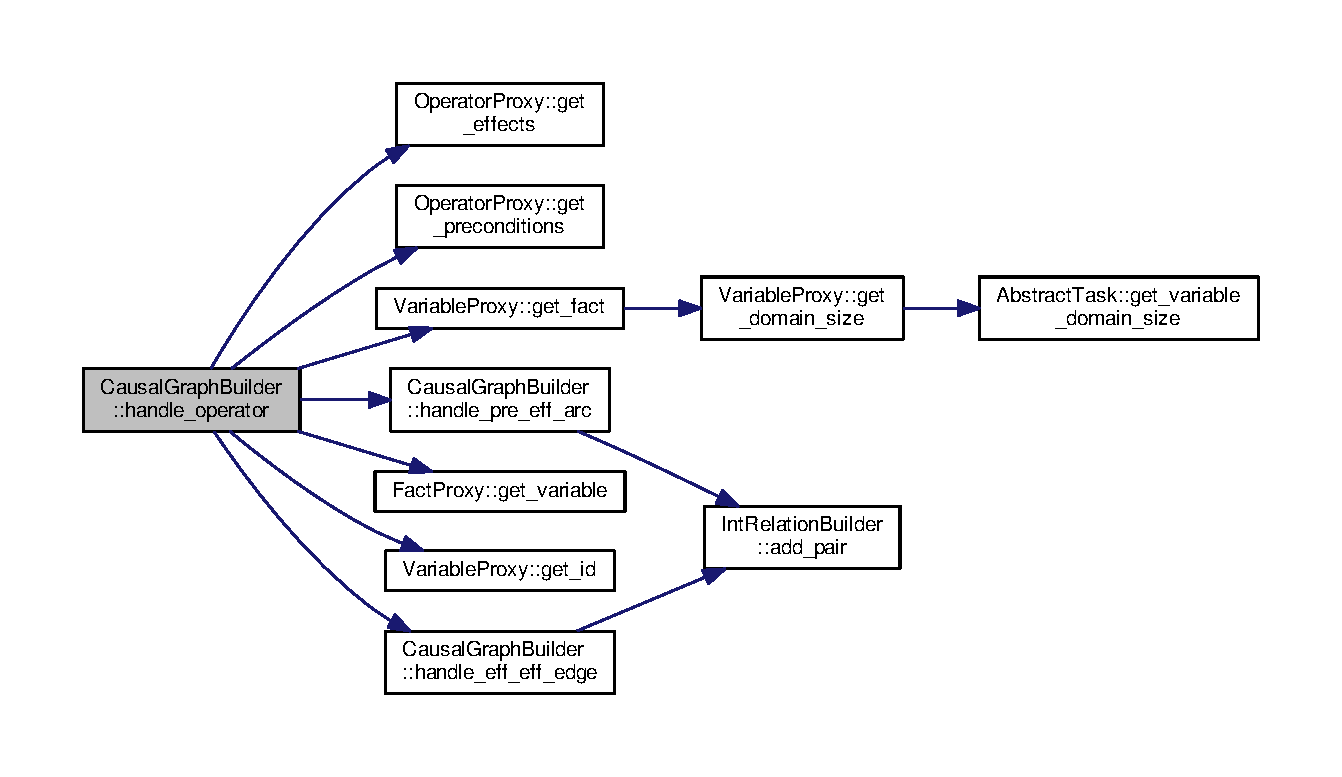
\includegraphics[width=350pt]{structCausalGraphBuilder_adae0f168f463cd392b11b93430e5c7f9_cgraph}
\end{center}
\end{figure}


\hypertarget{structCausalGraphBuilder_a07d4a8c5185dd840b766f10b4927c858}{\index{Causal\-Graph\-Builder@{Causal\-Graph\-Builder}!handle\-\_\-pre\-\_\-eff\-\_\-arc@{handle\-\_\-pre\-\_\-eff\-\_\-arc}}
\index{handle\-\_\-pre\-\_\-eff\-\_\-arc@{handle\-\_\-pre\-\_\-eff\-\_\-arc}!CausalGraphBuilder@{Causal\-Graph\-Builder}}
\subsubsection[{handle\-\_\-pre\-\_\-eff\-\_\-arc}]{\setlength{\rightskip}{0pt plus 5cm}void Causal\-Graph\-Builder\-::handle\-\_\-pre\-\_\-eff\-\_\-arc (
\begin{DoxyParamCaption}
\item[{int}]{u, }
\item[{int}]{v}
\end{DoxyParamCaption}
)\hspace{0.3cm}{\ttfamily [inline]}}}\label{structCausalGraphBuilder_a07d4a8c5185dd840b766f10b4927c858}


Here is the call graph for this function\-:
\nopagebreak
\begin{figure}[H]
\begin{center}
\leavevmode
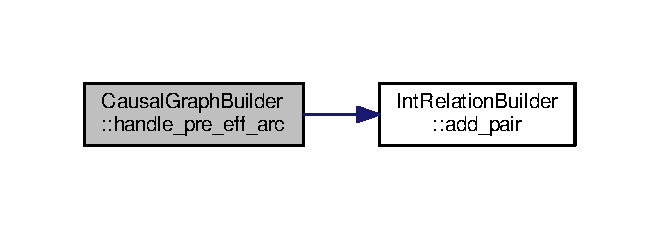
\includegraphics[width=316pt]{structCausalGraphBuilder_a07d4a8c5185dd840b766f10b4927c858_cgraph}
\end{center}
\end{figure}




\subsection{Member Data Documentation}
\hypertarget{structCausalGraphBuilder_a3320af04c6485bdbf93345cf2e9cfeb1}{\index{Causal\-Graph\-Builder@{Causal\-Graph\-Builder}!eff\-\_\-eff\-\_\-builder@{eff\-\_\-eff\-\_\-builder}}
\index{eff\-\_\-eff\-\_\-builder@{eff\-\_\-eff\-\_\-builder}!CausalGraphBuilder@{Causal\-Graph\-Builder}}
\subsubsection[{eff\-\_\-eff\-\_\-builder}]{\setlength{\rightskip}{0pt plus 5cm}{\bf Int\-Relation\-Builder} Causal\-Graph\-Builder\-::eff\-\_\-eff\-\_\-builder}}\label{structCausalGraphBuilder_a3320af04c6485bdbf93345cf2e9cfeb1}
\hypertarget{structCausalGraphBuilder_a773e4b6bc40fc74653a9d695f9983892}{\index{Causal\-Graph\-Builder@{Causal\-Graph\-Builder}!eff\-\_\-pre\-\_\-builder@{eff\-\_\-pre\-\_\-builder}}
\index{eff\-\_\-pre\-\_\-builder@{eff\-\_\-pre\-\_\-builder}!CausalGraphBuilder@{Causal\-Graph\-Builder}}
\subsubsection[{eff\-\_\-pre\-\_\-builder}]{\setlength{\rightskip}{0pt plus 5cm}{\bf Int\-Relation\-Builder} Causal\-Graph\-Builder\-::eff\-\_\-pre\-\_\-builder}}\label{structCausalGraphBuilder_a773e4b6bc40fc74653a9d695f9983892}
\hypertarget{structCausalGraphBuilder_a87a37c506c86e0e1332638066ac516e9}{\index{Causal\-Graph\-Builder@{Causal\-Graph\-Builder}!pre\-\_\-eff\-\_\-builder@{pre\-\_\-eff\-\_\-builder}}
\index{pre\-\_\-eff\-\_\-builder@{pre\-\_\-eff\-\_\-builder}!CausalGraphBuilder@{Causal\-Graph\-Builder}}
\subsubsection[{pre\-\_\-eff\-\_\-builder}]{\setlength{\rightskip}{0pt plus 5cm}{\bf Int\-Relation\-Builder} Causal\-Graph\-Builder\-::pre\-\_\-eff\-\_\-builder}}\label{structCausalGraphBuilder_a87a37c506c86e0e1332638066ac516e9}
\hypertarget{structCausalGraphBuilder_a916b1495bcd680ca74c216e49187fede}{\index{Causal\-Graph\-Builder@{Causal\-Graph\-Builder}!pred\-\_\-builder@{pred\-\_\-builder}}
\index{pred\-\_\-builder@{pred\-\_\-builder}!CausalGraphBuilder@{Causal\-Graph\-Builder}}
\subsubsection[{pred\-\_\-builder}]{\setlength{\rightskip}{0pt plus 5cm}{\bf Int\-Relation\-Builder} Causal\-Graph\-Builder\-::pred\-\_\-builder}}\label{structCausalGraphBuilder_a916b1495bcd680ca74c216e49187fede}
\hypertarget{structCausalGraphBuilder_a9a722f3782f6737608fd4b5fc8d9ea4e}{\index{Causal\-Graph\-Builder@{Causal\-Graph\-Builder}!succ\-\_\-builder@{succ\-\_\-builder}}
\index{succ\-\_\-builder@{succ\-\_\-builder}!CausalGraphBuilder@{Causal\-Graph\-Builder}}
\subsubsection[{succ\-\_\-builder}]{\setlength{\rightskip}{0pt plus 5cm}{\bf Int\-Relation\-Builder} Causal\-Graph\-Builder\-::succ\-\_\-builder}}\label{structCausalGraphBuilder_a9a722f3782f6737608fd4b5fc8d9ea4e}


The documentation for this struct was generated from the following file\-:\begin{DoxyCompactItemize}
\item 
\hyperlink{causal__graph_8cc}{causal\-\_\-graph.\-cc}\end{DoxyCompactItemize}

\hypertarget{classCGCache}{\section{C\-G\-Cache Class Reference}
\label{classCGCache}\index{C\-G\-Cache@{C\-G\-Cache}}
}


{\ttfamily \#include $<$cg\-\_\-cache.\-h$>$}

\subsection*{Public Member Functions}
\begin{DoxyCompactItemize}
\item 
\hyperlink{classCGCache_a96588e34b4c394b39462644711a55bdb}{C\-G\-Cache} ()
\item 
\hyperlink{classCGCache_a84abfac03826660e8b152f3e3b3e5dfb}{$\sim$\-C\-G\-Cache} ()
\item 
bool \hyperlink{classCGCache_a58802d9e1f1dad72bc2b15b89535f196}{is\-\_\-cached} (int var) const 
\item 
int \hyperlink{classCGCache_a54540ea4a44f5a2c29caa8883488a84d}{lookup} (int var, const \hyperlink{classGlobalState}{Global\-State} \&state, int from\-\_\-val, int to\-\_\-val) const 
\item 
void \hyperlink{classCGCache_a7677ea7457943d4081ae022ec58d5351}{store} (int var, const \hyperlink{classGlobalState}{Global\-State} \&state, int from\-\_\-val, int to\-\_\-val, int cost)
\item 
\hyperlink{structValueTransitionLabel}{Value\-Transition\-Label} $\ast$ \hyperlink{classCGCache_a5077434a3ab7427d9e0b13e01433be23}{lookup\-\_\-helpful\-\_\-transition} (int var, const \hyperlink{classGlobalState}{Global\-State} \&state, int from\-\_\-val, int to\-\_\-val) const 
\item 
void \hyperlink{classCGCache_ab9b77e6216328b13483854e6e68dc328}{store\-\_\-helpful\-\_\-transition} (int var, const \hyperlink{classGlobalState}{Global\-State} \&state, int from\-\_\-val, int to\-\_\-val, \hyperlink{structValueTransitionLabel}{Value\-Transition\-Label} $\ast$helpful\-\_\-transition)
\end{DoxyCompactItemize}
\subsection*{Static Public Attributes}
\begin{DoxyCompactItemize}
\item 
static const int \hyperlink{classCGCache_a171dd509e27a99afba696afe0c680b6d}{N\-O\-T\-\_\-\-C\-O\-M\-P\-U\-T\-E\-D} = -\/2
\end{DoxyCompactItemize}


\subsection{Constructor \& Destructor Documentation}
\hypertarget{classCGCache_a96588e34b4c394b39462644711a55bdb}{\index{C\-G\-Cache@{C\-G\-Cache}!C\-G\-Cache@{C\-G\-Cache}}
\index{C\-G\-Cache@{C\-G\-Cache}!CGCache@{C\-G\-Cache}}
\subsubsection[{C\-G\-Cache}]{\setlength{\rightskip}{0pt plus 5cm}C\-G\-Cache\-::\-C\-G\-Cache (
\begin{DoxyParamCaption}
{}
\end{DoxyParamCaption}
)}}\label{classCGCache_a96588e34b4c394b39462644711a55bdb}


Here is the call graph for this function\-:
\nopagebreak
\begin{figure}[H]
\begin{center}
\leavevmode
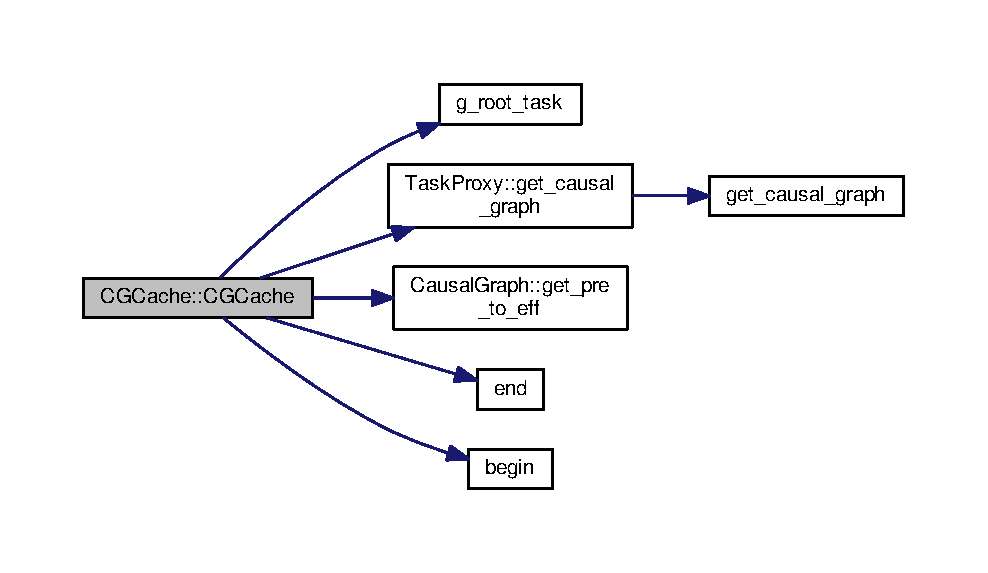
\includegraphics[width=350pt]{classCGCache_a96588e34b4c394b39462644711a55bdb_cgraph}
\end{center}
\end{figure}


\hypertarget{classCGCache_a84abfac03826660e8b152f3e3b3e5dfb}{\index{C\-G\-Cache@{C\-G\-Cache}!$\sim$\-C\-G\-Cache@{$\sim$\-C\-G\-Cache}}
\index{$\sim$\-C\-G\-Cache@{$\sim$\-C\-G\-Cache}!CGCache@{C\-G\-Cache}}
\subsubsection[{$\sim$\-C\-G\-Cache}]{\setlength{\rightskip}{0pt plus 5cm}C\-G\-Cache\-::$\sim$\-C\-G\-Cache (
\begin{DoxyParamCaption}
{}
\end{DoxyParamCaption}
)}}\label{classCGCache_a84abfac03826660e8b152f3e3b3e5dfb}


\subsection{Member Function Documentation}
\hypertarget{classCGCache_a58802d9e1f1dad72bc2b15b89535f196}{\index{C\-G\-Cache@{C\-G\-Cache}!is\-\_\-cached@{is\-\_\-cached}}
\index{is\-\_\-cached@{is\-\_\-cached}!CGCache@{C\-G\-Cache}}
\subsubsection[{is\-\_\-cached}]{\setlength{\rightskip}{0pt plus 5cm}bool C\-G\-Cache\-::is\-\_\-cached (
\begin{DoxyParamCaption}
\item[{int}]{var}
\end{DoxyParamCaption}
) const\hspace{0.3cm}{\ttfamily [inline]}}}\label{classCGCache_a58802d9e1f1dad72bc2b15b89535f196}
\hypertarget{classCGCache_a54540ea4a44f5a2c29caa8883488a84d}{\index{C\-G\-Cache@{C\-G\-Cache}!lookup@{lookup}}
\index{lookup@{lookup}!CGCache@{C\-G\-Cache}}
\subsubsection[{lookup}]{\setlength{\rightskip}{0pt plus 5cm}int C\-G\-Cache\-::lookup (
\begin{DoxyParamCaption}
\item[{int}]{var, }
\item[{const {\bf Global\-State} \&}]{state, }
\item[{int}]{from\-\_\-val, }
\item[{int}]{to\-\_\-val}
\end{DoxyParamCaption}
) const\hspace{0.3cm}{\ttfamily [inline]}}}\label{classCGCache_a54540ea4a44f5a2c29caa8883488a84d}
\hypertarget{classCGCache_a5077434a3ab7427d9e0b13e01433be23}{\index{C\-G\-Cache@{C\-G\-Cache}!lookup\-\_\-helpful\-\_\-transition@{lookup\-\_\-helpful\-\_\-transition}}
\index{lookup\-\_\-helpful\-\_\-transition@{lookup\-\_\-helpful\-\_\-transition}!CGCache@{C\-G\-Cache}}
\subsubsection[{lookup\-\_\-helpful\-\_\-transition}]{\setlength{\rightskip}{0pt plus 5cm}{\bf Value\-Transition\-Label}$\ast$ C\-G\-Cache\-::lookup\-\_\-helpful\-\_\-transition (
\begin{DoxyParamCaption}
\item[{int}]{var, }
\item[{const {\bf Global\-State} \&}]{state, }
\item[{int}]{from\-\_\-val, }
\item[{int}]{to\-\_\-val}
\end{DoxyParamCaption}
) const\hspace{0.3cm}{\ttfamily [inline]}}}\label{classCGCache_a5077434a3ab7427d9e0b13e01433be23}
\hypertarget{classCGCache_a7677ea7457943d4081ae022ec58d5351}{\index{C\-G\-Cache@{C\-G\-Cache}!store@{store}}
\index{store@{store}!CGCache@{C\-G\-Cache}}
\subsubsection[{store}]{\setlength{\rightskip}{0pt plus 5cm}void C\-G\-Cache\-::store (
\begin{DoxyParamCaption}
\item[{int}]{var, }
\item[{const {\bf Global\-State} \&}]{state, }
\item[{int}]{from\-\_\-val, }
\item[{int}]{to\-\_\-val, }
\item[{int}]{cost}
\end{DoxyParamCaption}
)\hspace{0.3cm}{\ttfamily [inline]}}}\label{classCGCache_a7677ea7457943d4081ae022ec58d5351}
\hypertarget{classCGCache_ab9b77e6216328b13483854e6e68dc328}{\index{C\-G\-Cache@{C\-G\-Cache}!store\-\_\-helpful\-\_\-transition@{store\-\_\-helpful\-\_\-transition}}
\index{store\-\_\-helpful\-\_\-transition@{store\-\_\-helpful\-\_\-transition}!CGCache@{C\-G\-Cache}}
\subsubsection[{store\-\_\-helpful\-\_\-transition}]{\setlength{\rightskip}{0pt plus 5cm}void C\-G\-Cache\-::store\-\_\-helpful\-\_\-transition (
\begin{DoxyParamCaption}
\item[{int}]{var, }
\item[{const {\bf Global\-State} \&}]{state, }
\item[{int}]{from\-\_\-val, }
\item[{int}]{to\-\_\-val, }
\item[{{\bf Value\-Transition\-Label} $\ast$}]{helpful\-\_\-transition}
\end{DoxyParamCaption}
)\hspace{0.3cm}{\ttfamily [inline]}}}\label{classCGCache_ab9b77e6216328b13483854e6e68dc328}


\subsection{Member Data Documentation}
\hypertarget{classCGCache_a171dd509e27a99afba696afe0c680b6d}{\index{C\-G\-Cache@{C\-G\-Cache}!N\-O\-T\-\_\-\-C\-O\-M\-P\-U\-T\-E\-D@{N\-O\-T\-\_\-\-C\-O\-M\-P\-U\-T\-E\-D}}
\index{N\-O\-T\-\_\-\-C\-O\-M\-P\-U\-T\-E\-D@{N\-O\-T\-\_\-\-C\-O\-M\-P\-U\-T\-E\-D}!CGCache@{C\-G\-Cache}}
\subsubsection[{N\-O\-T\-\_\-\-C\-O\-M\-P\-U\-T\-E\-D}]{\setlength{\rightskip}{0pt plus 5cm}const int C\-G\-Cache\-::\-N\-O\-T\-\_\-\-C\-O\-M\-P\-U\-T\-E\-D = -\/2\hspace{0.3cm}{\ttfamily [static]}}}\label{classCGCache_a171dd509e27a99afba696afe0c680b6d}


The documentation for this class was generated from the following files\-:\begin{DoxyCompactItemize}
\item 
\hyperlink{cg__cache_8h}{cg\-\_\-cache.\-h}\item 
\hyperlink{cg__cache_8cc}{cg\-\_\-cache.\-cc}\end{DoxyCompactItemize}

\hypertarget{classCGHeuristic}{\section{C\-G\-Heuristic Class Reference}
\label{classCGHeuristic}\index{C\-G\-Heuristic@{C\-G\-Heuristic}}
}


{\ttfamily \#include $<$cg\-\_\-heuristic.\-h$>$}



Inheritance diagram for C\-G\-Heuristic\-:
\nopagebreak
\begin{figure}[H]
\begin{center}
\leavevmode
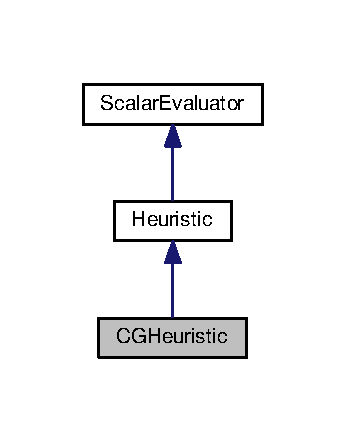
\includegraphics[width=166pt]{classCGHeuristic__inherit__graph}
\end{center}
\end{figure}


Collaboration diagram for C\-G\-Heuristic\-:
\nopagebreak
\begin{figure}[H]
\begin{center}
\leavevmode
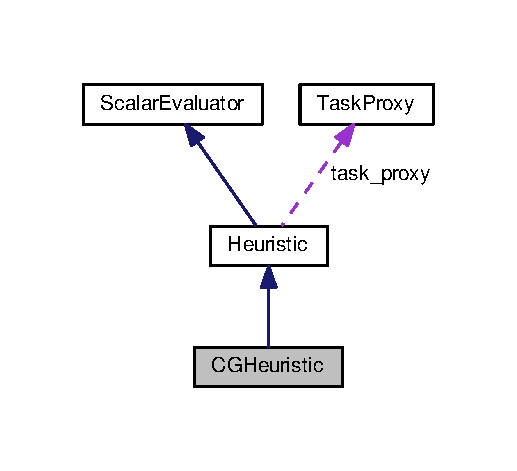
\includegraphics[width=248pt]{classCGHeuristic__coll__graph}
\end{center}
\end{figure}
\subsection*{Public Member Functions}
\begin{DoxyCompactItemize}
\item 
\hyperlink{classCGHeuristic_a1c4c671e749df50cc75cf1f5f4a36233}{C\-G\-Heuristic} (const \hyperlink{classOptions}{Options} \&opts)
\item 
\hyperlink{classCGHeuristic_a9f8a37d085038ed5388c5351adcadc42}{$\sim$\-C\-G\-Heuristic} ()
\item 
virtual bool \hyperlink{classCGHeuristic_a35e572c29eff7b1ce661fafac90c46d5}{dead\-\_\-ends\-\_\-are\-\_\-reliable} () const 
\end{DoxyCompactItemize}
\subsection*{Protected Member Functions}
\begin{DoxyCompactItemize}
\item 
virtual void \hyperlink{classCGHeuristic_a41af92f82ef6d2f57552e894cb1d50fb}{initialize} ()
\item 
virtual int \hyperlink{classCGHeuristic_ad2e02bf90acf0452245fece28aa78e97}{compute\-\_\-heuristic} (const \hyperlink{classGlobalState}{Global\-State} \&state)
\end{DoxyCompactItemize}
\subsection*{Additional Inherited Members}


\subsection{Constructor \& Destructor Documentation}
\hypertarget{classCGHeuristic_a1c4c671e749df50cc75cf1f5f4a36233}{\index{C\-G\-Heuristic@{C\-G\-Heuristic}!C\-G\-Heuristic@{C\-G\-Heuristic}}
\index{C\-G\-Heuristic@{C\-G\-Heuristic}!CGHeuristic@{C\-G\-Heuristic}}
\subsubsection[{C\-G\-Heuristic}]{\setlength{\rightskip}{0pt plus 5cm}C\-G\-Heuristic\-::\-C\-G\-Heuristic (
\begin{DoxyParamCaption}
\item[{const {\bf Options} \&}]{opts}
\end{DoxyParamCaption}
)}}\label{classCGHeuristic_a1c4c671e749df50cc75cf1f5f4a36233}
\hypertarget{classCGHeuristic_a9f8a37d085038ed5388c5351adcadc42}{\index{C\-G\-Heuristic@{C\-G\-Heuristic}!$\sim$\-C\-G\-Heuristic@{$\sim$\-C\-G\-Heuristic}}
\index{$\sim$\-C\-G\-Heuristic@{$\sim$\-C\-G\-Heuristic}!CGHeuristic@{C\-G\-Heuristic}}
\subsubsection[{$\sim$\-C\-G\-Heuristic}]{\setlength{\rightskip}{0pt plus 5cm}C\-G\-Heuristic\-::$\sim$\-C\-G\-Heuristic (
\begin{DoxyParamCaption}
{}
\end{DoxyParamCaption}
)}}\label{classCGHeuristic_a9f8a37d085038ed5388c5351adcadc42}


\subsection{Member Function Documentation}
\hypertarget{classCGHeuristic_ad2e02bf90acf0452245fece28aa78e97}{\index{C\-G\-Heuristic@{C\-G\-Heuristic}!compute\-\_\-heuristic@{compute\-\_\-heuristic}}
\index{compute\-\_\-heuristic@{compute\-\_\-heuristic}!CGHeuristic@{C\-G\-Heuristic}}
\subsubsection[{compute\-\_\-heuristic}]{\setlength{\rightskip}{0pt plus 5cm}int C\-G\-Heuristic\-::compute\-\_\-heuristic (
\begin{DoxyParamCaption}
\item[{const {\bf Global\-State} \&}]{state}
\end{DoxyParamCaption}
)\hspace{0.3cm}{\ttfamily [protected]}, {\ttfamily [virtual]}}}\label{classCGHeuristic_ad2e02bf90acf0452245fece28aa78e97}


Implements \hyperlink{classHeuristic_a4fd4e087281805e0e76a814e06d4e506}{Heuristic}.

\hypertarget{classCGHeuristic_a35e572c29eff7b1ce661fafac90c46d5}{\index{C\-G\-Heuristic@{C\-G\-Heuristic}!dead\-\_\-ends\-\_\-are\-\_\-reliable@{dead\-\_\-ends\-\_\-are\-\_\-reliable}}
\index{dead\-\_\-ends\-\_\-are\-\_\-reliable@{dead\-\_\-ends\-\_\-are\-\_\-reliable}!CGHeuristic@{C\-G\-Heuristic}}
\subsubsection[{dead\-\_\-ends\-\_\-are\-\_\-reliable}]{\setlength{\rightskip}{0pt plus 5cm}bool C\-G\-Heuristic\-::dead\-\_\-ends\-\_\-are\-\_\-reliable (
\begin{DoxyParamCaption}
{}
\end{DoxyParamCaption}
) const\hspace{0.3cm}{\ttfamily [virtual]}}}\label{classCGHeuristic_a35e572c29eff7b1ce661fafac90c46d5}


Reimplemented from \hyperlink{classScalarEvaluator_aa4534363976871466aa2be88f82e1a74}{Scalar\-Evaluator}.

\hypertarget{classCGHeuristic_a41af92f82ef6d2f57552e894cb1d50fb}{\index{C\-G\-Heuristic@{C\-G\-Heuristic}!initialize@{initialize}}
\index{initialize@{initialize}!CGHeuristic@{C\-G\-Heuristic}}
\subsubsection[{initialize}]{\setlength{\rightskip}{0pt plus 5cm}void C\-G\-Heuristic\-::initialize (
\begin{DoxyParamCaption}
{}
\end{DoxyParamCaption}
)\hspace{0.3cm}{\ttfamily [protected]}, {\ttfamily [virtual]}}}\label{classCGHeuristic_a41af92f82ef6d2f57552e894cb1d50fb}


Reimplemented from \hyperlink{classHeuristic_a26e75bad1d806657c0ed274b4fe72f0a}{Heuristic}.



The documentation for this class was generated from the following files\-:\begin{DoxyCompactItemize}
\item 
\hyperlink{cg__heuristic_8h}{cg\-\_\-heuristic.\-h}\item 
\hyperlink{cg__heuristic_8cc}{cg\-\_\-heuristic.\-cc}\end{DoxyCompactItemize}

\hypertarget{classCombiningEvaluator}{\section{Combining\-Evaluator Class Reference}
\label{classCombiningEvaluator}\index{Combining\-Evaluator@{Combining\-Evaluator}}
}


{\ttfamily \#include $<$combining\-\_\-evaluator.\-h$>$}



Inheritance diagram for Combining\-Evaluator\-:
\nopagebreak
\begin{figure}[H]
\begin{center}
\leavevmode
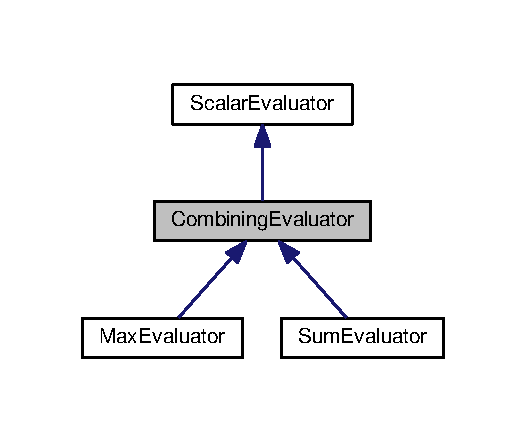
\includegraphics[width=253pt]{classCombiningEvaluator__inherit__graph}
\end{center}
\end{figure}


Collaboration diagram for Combining\-Evaluator\-:
\nopagebreak
\begin{figure}[H]
\begin{center}
\leavevmode
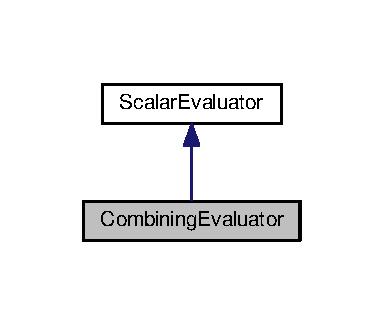
\includegraphics[width=184pt]{classCombiningEvaluator__coll__graph}
\end{center}
\end{figure}
\subsection*{Public Member Functions}
\begin{DoxyCompactItemize}
\item 
\hyperlink{classCombiningEvaluator_ab0d3e60b90a84ca1f6bba21670ea4268}{Combining\-Evaluator} (const std\-::vector$<$ \hyperlink{classScalarEvaluator}{Scalar\-Evaluator} $\ast$ $>$ \&subevaluators\-\_\-)
\item 
virtual \hyperlink{classCombiningEvaluator_a2cfc4161494028950a1d46be718701aa}{$\sim$\-Combining\-Evaluator} () override
\item 
virtual bool \hyperlink{classCombiningEvaluator_a72f61f835e02b716d02734a65b1c7d99}{dead\-\_\-ends\-\_\-are\-\_\-reliable} () const override
\item 
virtual \hyperlink{classEvaluationResult}{Evaluation\-Result} \hyperlink{classCombiningEvaluator_a9da792d602f409634bea4ceb32421369}{compute\-\_\-result} (\hyperlink{classEvaluationContext}{Evaluation\-Context} \&eval\-\_\-context) override
\item 
virtual void \hyperlink{classCombiningEvaluator_acaba3e4f6375cba36fedbefe5a9bdea1}{get\-\_\-involved\-\_\-heuristics} (std\-::set$<$ \hyperlink{classHeuristic}{Heuristic} $\ast$ $>$ \&hset) override
\end{DoxyCompactItemize}
\subsection*{Protected Member Functions}
\begin{DoxyCompactItemize}
\item 
virtual int \hyperlink{classCombiningEvaluator_ae88080950f68d03c5b9e7c96cddfd7a9}{combine\-\_\-values} (const std\-::vector$<$ int $>$ \&values)=0
\end{DoxyCompactItemize}


\subsection{Constructor \& Destructor Documentation}
\hypertarget{classCombiningEvaluator_ab0d3e60b90a84ca1f6bba21670ea4268}{\index{Combining\-Evaluator@{Combining\-Evaluator}!Combining\-Evaluator@{Combining\-Evaluator}}
\index{Combining\-Evaluator@{Combining\-Evaluator}!CombiningEvaluator@{Combining\-Evaluator}}
\subsubsection[{Combining\-Evaluator}]{\setlength{\rightskip}{0pt plus 5cm}Combining\-Evaluator\-::\-Combining\-Evaluator (
\begin{DoxyParamCaption}
\item[{const std\-::vector$<$ {\bf Scalar\-Evaluator} $\ast$ $>$ \&}]{subevaluators\-\_\-}
\end{DoxyParamCaption}
)\hspace{0.3cm}{\ttfamily [explicit]}}}\label{classCombiningEvaluator_ab0d3e60b90a84ca1f6bba21670ea4268}
\hypertarget{classCombiningEvaluator_a2cfc4161494028950a1d46be718701aa}{\index{Combining\-Evaluator@{Combining\-Evaluator}!$\sim$\-Combining\-Evaluator@{$\sim$\-Combining\-Evaluator}}
\index{$\sim$\-Combining\-Evaluator@{$\sim$\-Combining\-Evaluator}!CombiningEvaluator@{Combining\-Evaluator}}
\subsubsection[{$\sim$\-Combining\-Evaluator}]{\setlength{\rightskip}{0pt plus 5cm}Combining\-Evaluator\-::$\sim$\-Combining\-Evaluator (
\begin{DoxyParamCaption}
{}
\end{DoxyParamCaption}
)\hspace{0.3cm}{\ttfamily [override]}, {\ttfamily [virtual]}}}\label{classCombiningEvaluator_a2cfc4161494028950a1d46be718701aa}


\subsection{Member Function Documentation}
\hypertarget{classCombiningEvaluator_ae88080950f68d03c5b9e7c96cddfd7a9}{\index{Combining\-Evaluator@{Combining\-Evaluator}!combine\-\_\-values@{combine\-\_\-values}}
\index{combine\-\_\-values@{combine\-\_\-values}!CombiningEvaluator@{Combining\-Evaluator}}
\subsubsection[{combine\-\_\-values}]{\setlength{\rightskip}{0pt plus 5cm}virtual int Combining\-Evaluator\-::combine\-\_\-values (
\begin{DoxyParamCaption}
\item[{const std\-::vector$<$ int $>$ \&}]{values}
\end{DoxyParamCaption}
)\hspace{0.3cm}{\ttfamily [protected]}, {\ttfamily [pure virtual]}}}\label{classCombiningEvaluator_ae88080950f68d03c5b9e7c96cddfd7a9}


Implemented in \hyperlink{classSumEvaluator_a7ce904c3d881887263f3e655304a5f6b}{Sum\-Evaluator}, and \hyperlink{classMaxEvaluator_ae4e0e2dae5d2572c91dd2b6ad616fdfd}{Max\-Evaluator}.

\hypertarget{classCombiningEvaluator_a9da792d602f409634bea4ceb32421369}{\index{Combining\-Evaluator@{Combining\-Evaluator}!compute\-\_\-result@{compute\-\_\-result}}
\index{compute\-\_\-result@{compute\-\_\-result}!CombiningEvaluator@{Combining\-Evaluator}}
\subsubsection[{compute\-\_\-result}]{\setlength{\rightskip}{0pt plus 5cm}{\bf Evaluation\-Result} Combining\-Evaluator\-::compute\-\_\-result (
\begin{DoxyParamCaption}
\item[{{\bf Evaluation\-Context} \&}]{eval\-\_\-context}
\end{DoxyParamCaption}
)\hspace{0.3cm}{\ttfamily [override]}, {\ttfamily [virtual]}}}\label{classCombiningEvaluator_a9da792d602f409634bea4ceb32421369}


Implements \hyperlink{classScalarEvaluator_a8ffb99b0f8f63e34183a3245a247a9ec}{Scalar\-Evaluator}.



Here is the call graph for this function\-:
\nopagebreak
\begin{figure}[H]
\begin{center}
\leavevmode
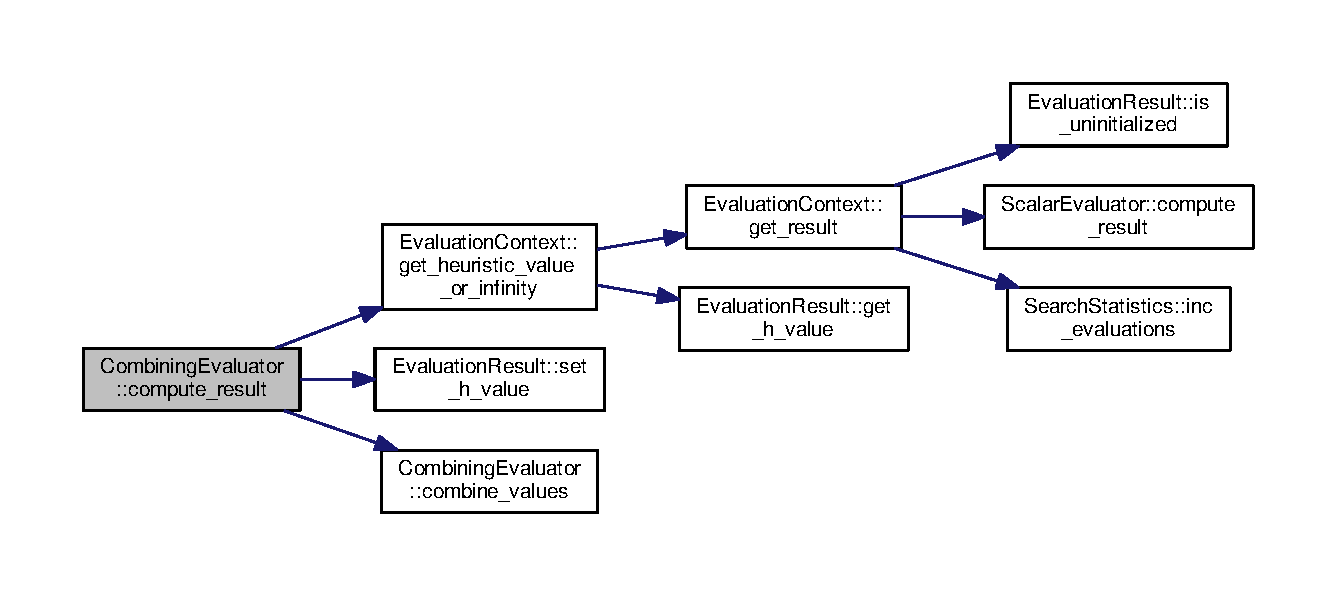
\includegraphics[width=350pt]{classCombiningEvaluator_a9da792d602f409634bea4ceb32421369_cgraph}
\end{center}
\end{figure}


\hypertarget{classCombiningEvaluator_a72f61f835e02b716d02734a65b1c7d99}{\index{Combining\-Evaluator@{Combining\-Evaluator}!dead\-\_\-ends\-\_\-are\-\_\-reliable@{dead\-\_\-ends\-\_\-are\-\_\-reliable}}
\index{dead\-\_\-ends\-\_\-are\-\_\-reliable@{dead\-\_\-ends\-\_\-are\-\_\-reliable}!CombiningEvaluator@{Combining\-Evaluator}}
\subsubsection[{dead\-\_\-ends\-\_\-are\-\_\-reliable}]{\setlength{\rightskip}{0pt plus 5cm}bool Combining\-Evaluator\-::dead\-\_\-ends\-\_\-are\-\_\-reliable (
\begin{DoxyParamCaption}
{}
\end{DoxyParamCaption}
) const\hspace{0.3cm}{\ttfamily [override]}, {\ttfamily [virtual]}}}\label{classCombiningEvaluator_a72f61f835e02b716d02734a65b1c7d99}


Reimplemented from \hyperlink{classScalarEvaluator_aa4534363976871466aa2be88f82e1a74}{Scalar\-Evaluator}.

\hypertarget{classCombiningEvaluator_acaba3e4f6375cba36fedbefe5a9bdea1}{\index{Combining\-Evaluator@{Combining\-Evaluator}!get\-\_\-involved\-\_\-heuristics@{get\-\_\-involved\-\_\-heuristics}}
\index{get\-\_\-involved\-\_\-heuristics@{get\-\_\-involved\-\_\-heuristics}!CombiningEvaluator@{Combining\-Evaluator}}
\subsubsection[{get\-\_\-involved\-\_\-heuristics}]{\setlength{\rightskip}{0pt plus 5cm}void Combining\-Evaluator\-::get\-\_\-involved\-\_\-heuristics (
\begin{DoxyParamCaption}
\item[{std\-::set$<$ {\bf Heuristic} $\ast$ $>$ \&}]{hset}
\end{DoxyParamCaption}
)\hspace{0.3cm}{\ttfamily [override]}, {\ttfamily [virtual]}}}\label{classCombiningEvaluator_acaba3e4f6375cba36fedbefe5a9bdea1}


Implements \hyperlink{classScalarEvaluator_a23640092537e3403bbc5b40389f7f253}{Scalar\-Evaluator}.



The documentation for this class was generated from the following files\-:\begin{DoxyCompactItemize}
\item 
\hyperlink{combining__evaluator_8h}{combining\-\_\-evaluator.\-h}\item 
\hyperlink{combining__evaluator_8cc}{combining\-\_\-evaluator.\-cc}\end{DoxyCompactItemize}

\hypertarget{classConditionsProxy}{\section{Conditions\-Proxy Class Reference}
\label{classConditionsProxy}\index{Conditions\-Proxy@{Conditions\-Proxy}}
}


{\ttfamily \#include $<$task\-\_\-proxy.\-h$>$}



Inheritance diagram for Conditions\-Proxy\-:
\nopagebreak
\begin{figure}[H]
\begin{center}
\leavevmode
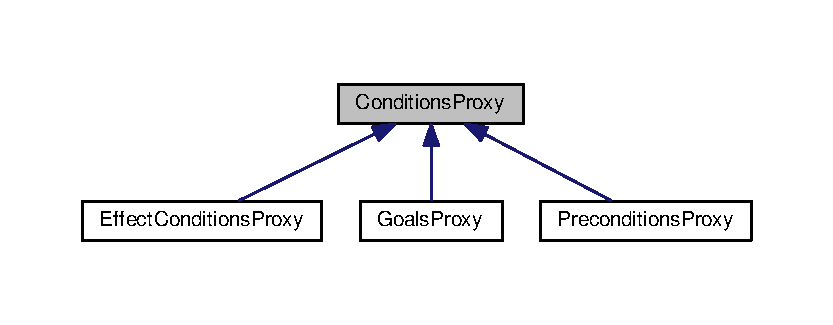
\includegraphics[width=350pt]{classConditionsProxy__inherit__graph}
\end{center}
\end{figure}


Collaboration diagram for Conditions\-Proxy\-:
\nopagebreak
\begin{figure}[H]
\begin{center}
\leavevmode
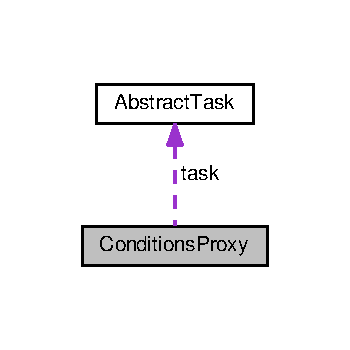
\includegraphics[width=168pt]{classConditionsProxy__coll__graph}
\end{center}
\end{figure}
\subsection*{Public Types}
\begin{DoxyCompactItemize}
\item 
using \hyperlink{classConditionsProxy_a10602694ed5094da8bdc7e6e3167bf02}{Item\-Type} = \hyperlink{classFactProxy}{Fact\-Proxy}
\end{DoxyCompactItemize}
\subsection*{Public Member Functions}
\begin{DoxyCompactItemize}
\item 
\hyperlink{classConditionsProxy_a0f4d3d6bb5b20b0689d094141967405a}{Conditions\-Proxy} (const \hyperlink{classAbstractTask}{Abstract\-Task} \&\hyperlink{classConditionsProxy_a8e8c904bd5dc370a7239ec7495dc0dfe}{task})
\item 
virtual \hyperlink{classConditionsProxy_a77219c9e840f9d542428539677296cf9}{$\sim$\-Conditions\-Proxy} ()=default
\item 
virtual std\-::size\-\_\-t \hyperlink{classConditionsProxy_af0710776571971659082f0140e4cdba3}{size} () const =0
\item 
virtual \hyperlink{classFactProxy}{Fact\-Proxy} \hyperlink{classConditionsProxy_a558d807927b992bad3728268b7e8a533}{operator\mbox{[}$\,$\mbox{]}} (std\-::size\-\_\-t index) const =0
\item 
bool \hyperlink{classConditionsProxy_a1ee8f0ef3bf2eed02add56d417a10566}{empty} () const 
\end{DoxyCompactItemize}
\subsection*{Protected Attributes}
\begin{DoxyCompactItemize}
\item 
const \hyperlink{classAbstractTask}{Abstract\-Task} $\ast$ \hyperlink{classConditionsProxy_a8e8c904bd5dc370a7239ec7495dc0dfe}{task}
\end{DoxyCompactItemize}


\subsection{Member Typedef Documentation}
\hypertarget{classConditionsProxy_a10602694ed5094da8bdc7e6e3167bf02}{\index{Conditions\-Proxy@{Conditions\-Proxy}!Item\-Type@{Item\-Type}}
\index{Item\-Type@{Item\-Type}!ConditionsProxy@{Conditions\-Proxy}}
\subsubsection[{Item\-Type}]{\setlength{\rightskip}{0pt plus 5cm}using {\bf Conditions\-Proxy\-::\-Item\-Type} =  {\bf Fact\-Proxy}}}\label{classConditionsProxy_a10602694ed5094da8bdc7e6e3167bf02}


\subsection{Constructor \& Destructor Documentation}
\hypertarget{classConditionsProxy_a0f4d3d6bb5b20b0689d094141967405a}{\index{Conditions\-Proxy@{Conditions\-Proxy}!Conditions\-Proxy@{Conditions\-Proxy}}
\index{Conditions\-Proxy@{Conditions\-Proxy}!ConditionsProxy@{Conditions\-Proxy}}
\subsubsection[{Conditions\-Proxy}]{\setlength{\rightskip}{0pt plus 5cm}Conditions\-Proxy\-::\-Conditions\-Proxy (
\begin{DoxyParamCaption}
\item[{const {\bf Abstract\-Task} \&}]{task}
\end{DoxyParamCaption}
)\hspace{0.3cm}{\ttfamily [inline]}, {\ttfamily [explicit]}}}\label{classConditionsProxy_a0f4d3d6bb5b20b0689d094141967405a}
\hypertarget{classConditionsProxy_a77219c9e840f9d542428539677296cf9}{\index{Conditions\-Proxy@{Conditions\-Proxy}!$\sim$\-Conditions\-Proxy@{$\sim$\-Conditions\-Proxy}}
\index{$\sim$\-Conditions\-Proxy@{$\sim$\-Conditions\-Proxy}!ConditionsProxy@{Conditions\-Proxy}}
\subsubsection[{$\sim$\-Conditions\-Proxy}]{\setlength{\rightskip}{0pt plus 5cm}virtual Conditions\-Proxy\-::$\sim$\-Conditions\-Proxy (
\begin{DoxyParamCaption}
{}
\end{DoxyParamCaption}
)\hspace{0.3cm}{\ttfamily [virtual]}, {\ttfamily [default]}}}\label{classConditionsProxy_a77219c9e840f9d542428539677296cf9}


\subsection{Member Function Documentation}
\hypertarget{classConditionsProxy_a1ee8f0ef3bf2eed02add56d417a10566}{\index{Conditions\-Proxy@{Conditions\-Proxy}!empty@{empty}}
\index{empty@{empty}!ConditionsProxy@{Conditions\-Proxy}}
\subsubsection[{empty}]{\setlength{\rightskip}{0pt plus 5cm}bool Conditions\-Proxy\-::empty (
\begin{DoxyParamCaption}
{}
\end{DoxyParamCaption}
) const\hspace{0.3cm}{\ttfamily [inline]}}}\label{classConditionsProxy_a1ee8f0ef3bf2eed02add56d417a10566}


Here is the call graph for this function\-:
\nopagebreak
\begin{figure}[H]
\begin{center}
\leavevmode
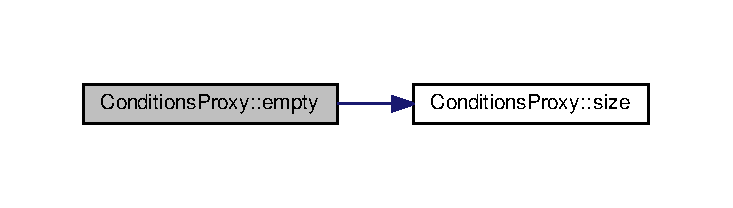
\includegraphics[width=350pt]{classConditionsProxy_a1ee8f0ef3bf2eed02add56d417a10566_cgraph}
\end{center}
\end{figure}


\hypertarget{classConditionsProxy_a558d807927b992bad3728268b7e8a533}{\index{Conditions\-Proxy@{Conditions\-Proxy}!operator\mbox{[}$\,$\mbox{]}@{operator[]}}
\index{operator\mbox{[}$\,$\mbox{]}@{operator[]}!ConditionsProxy@{Conditions\-Proxy}}
\subsubsection[{operator[]}]{\setlength{\rightskip}{0pt plus 5cm}virtual {\bf Fact\-Proxy} Conditions\-Proxy\-::operator\mbox{[}$\,$\mbox{]} (
\begin{DoxyParamCaption}
\item[{std\-::size\-\_\-t}]{index}
\end{DoxyParamCaption}
) const\hspace{0.3cm}{\ttfamily [pure virtual]}}}\label{classConditionsProxy_a558d807927b992bad3728268b7e8a533}


Implemented in \hyperlink{classGoalsProxy_aa976feb7b10e95fab32135a65e135247}{Goals\-Proxy}, \hyperlink{classEffectConditionsProxy_a9f41ffe872d125b643591f050e8ca69a}{Effect\-Conditions\-Proxy}, and \hyperlink{classPreconditionsProxy_ae350b0dfab627206414f3dc3a8a819ce}{Preconditions\-Proxy}.

\hypertarget{classConditionsProxy_af0710776571971659082f0140e4cdba3}{\index{Conditions\-Proxy@{Conditions\-Proxy}!size@{size}}
\index{size@{size}!ConditionsProxy@{Conditions\-Proxy}}
\subsubsection[{size}]{\setlength{\rightskip}{0pt plus 5cm}virtual std\-::size\-\_\-t Conditions\-Proxy\-::size (
\begin{DoxyParamCaption}
{}
\end{DoxyParamCaption}
) const\hspace{0.3cm}{\ttfamily [pure virtual]}}}\label{classConditionsProxy_af0710776571971659082f0140e4cdba3}


Implemented in \hyperlink{classGoalsProxy_abfc758e237e5ef8d56fd1e0c0f3eb6f8}{Goals\-Proxy}, \hyperlink{classEffectConditionsProxy_af447849d62079e622be08a68df7dab14}{Effect\-Conditions\-Proxy}, and \hyperlink{classPreconditionsProxy_a63cac56561ada0b576cff8f732a3a902}{Preconditions\-Proxy}.



\subsection{Member Data Documentation}
\hypertarget{classConditionsProxy_a8e8c904bd5dc370a7239ec7495dc0dfe}{\index{Conditions\-Proxy@{Conditions\-Proxy}!task@{task}}
\index{task@{task}!ConditionsProxy@{Conditions\-Proxy}}
\subsubsection[{task}]{\setlength{\rightskip}{0pt plus 5cm}const {\bf Abstract\-Task}$\ast$ Conditions\-Proxy\-::task\hspace{0.3cm}{\ttfamily [protected]}}}\label{classConditionsProxy_a8e8c904bd5dc370a7239ec7495dc0dfe}


The documentation for this class was generated from the following file\-:\begin{DoxyCompactItemize}
\item 
\hyperlink{task__proxy_8h}{task\-\_\-proxy.\-h}\end{DoxyCompactItemize}

\hypertarget{classPerStateInformation_1_1const__iterator}{\section{Per\-State\-Information$<$ Entry $>$\-:\-:const\-\_\-iterator Class Reference}
\label{classPerStateInformation_1_1const__iterator}\index{Per\-State\-Information$<$ Entry $>$\-::const\-\_\-iterator@{Per\-State\-Information$<$ Entry $>$\-::const\-\_\-iterator}}
}


{\ttfamily \#include $<$per\-\_\-state\-\_\-information.\-h$>$}



Inheritance diagram for Per\-State\-Information$<$ Entry $>$\-:\-:const\-\_\-iterator\-:
\nopagebreak
\begin{figure}[H]
\begin{center}
\leavevmode
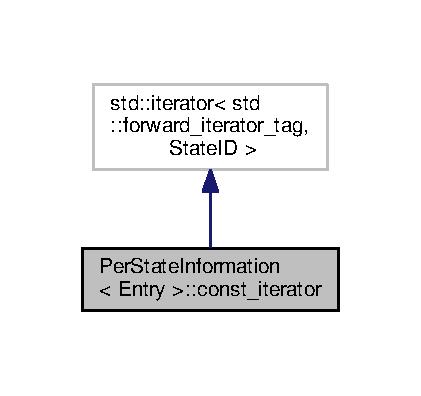
\includegraphics[width=202pt]{classPerStateInformation_1_1const__iterator__inherit__graph}
\end{center}
\end{figure}


Collaboration diagram for Per\-State\-Information$<$ Entry $>$\-:\-:const\-\_\-iterator\-:
\nopagebreak
\begin{figure}[H]
\begin{center}
\leavevmode
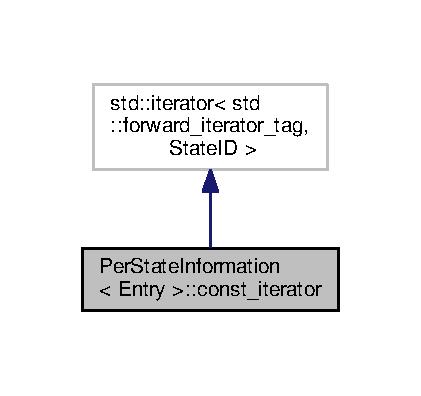
\includegraphics[width=202pt]{classPerStateInformation_1_1const__iterator__coll__graph}
\end{center}
\end{figure}
\subsection*{Public Member Functions}
\begin{DoxyCompactItemize}
\item 
\hyperlink{classPerStateInformation_1_1const__iterator_a2f355ee663a5a209b5aea6741da55f19}{const\-\_\-iterator} (const \hyperlink{classPerStateInformation_1_1const__iterator}{const\-\_\-iterator} \&other)
\item 
\hyperlink{classPerStateInformation_1_1const__iterator_a21d459dce06190484592edc47b1d7d24}{$\sim$const\-\_\-iterator} ()
\item 
\hyperlink{classPerStateInformation_1_1const__iterator}{const\-\_\-iterator} \& \hyperlink{classPerStateInformation_1_1const__iterator_a5c83a66ca45a375b52360e2773ea575b}{operator++} ()
\item 
\hyperlink{classPerStateInformation_1_1const__iterator}{const\-\_\-iterator} \hyperlink{classPerStateInformation_1_1const__iterator_a07fb0708c40615406279fb7ca382f698}{operator++} (int)
\item 
bool \hyperlink{classPerStateInformation_1_1const__iterator_a9e09cdff82fb1b6b669cd28d6ec8bb14}{operator==} (const \hyperlink{classPerStateInformation_1_1const__iterator}{const\-\_\-iterator} \&rhs)
\item 
bool \hyperlink{classPerStateInformation_1_1const__iterator_a1973f2f89e030f6132ac4e09625d7518}{operator!=} (const \hyperlink{classPerStateInformation_1_1const__iterator}{const\-\_\-iterator} \&rhs)
\item 
\hyperlink{classStateID}{State\-I\-D} \hyperlink{classPerStateInformation_1_1const__iterator_a69921e1a8df8b883b87acc0f35a8f280}{operator$\ast$} ()
\item 
\hyperlink{classStateID}{State\-I\-D} $\ast$ \hyperlink{classPerStateInformation_1_1const__iterator_ae2fa5a43e634d0036e97424bad5c1f18}{operator-\/$>$} ()
\end{DoxyCompactItemize}
\subsection*{Friends}
\begin{DoxyCompactItemize}
\item 
class \hyperlink{classPerStateInformation_1_1const__iterator_ae69462da21a4e3a3b602a69ebc4738c1}{Per\-State\-Information$<$ Entry $>$}
\end{DoxyCompactItemize}


\subsection{Constructor \& Destructor Documentation}
\hypertarget{classPerStateInformation_1_1const__iterator_a2f355ee663a5a209b5aea6741da55f19}{\index{Per\-State\-Information\-::const\-\_\-iterator@{Per\-State\-Information\-::const\-\_\-iterator}!const\-\_\-iterator@{const\-\_\-iterator}}
\index{const\-\_\-iterator@{const\-\_\-iterator}!PerStateInformation::const_iterator@{Per\-State\-Information\-::const\-\_\-iterator}}
\subsubsection[{const\-\_\-iterator}]{\setlength{\rightskip}{0pt plus 5cm}template$<$class Entry$>$ {\bf Per\-State\-Information}$<$ Entry $>$\-::const\-\_\-iterator\-::const\-\_\-iterator (
\begin{DoxyParamCaption}
\item[{const {\bf const\-\_\-iterator} \&}]{other}
\end{DoxyParamCaption}
)\hspace{0.3cm}{\ttfamily [inline]}}}\label{classPerStateInformation_1_1const__iterator_a2f355ee663a5a209b5aea6741da55f19}
\hypertarget{classPerStateInformation_1_1const__iterator_a21d459dce06190484592edc47b1d7d24}{\index{Per\-State\-Information\-::const\-\_\-iterator@{Per\-State\-Information\-::const\-\_\-iterator}!$\sim$const\-\_\-iterator@{$\sim$const\-\_\-iterator}}
\index{$\sim$const\-\_\-iterator@{$\sim$const\-\_\-iterator}!PerStateInformation::const_iterator@{Per\-State\-Information\-::const\-\_\-iterator}}
\subsubsection[{$\sim$const\-\_\-iterator}]{\setlength{\rightskip}{0pt plus 5cm}template$<$class Entry$>$ {\bf Per\-State\-Information}$<$ Entry $>$\-::const\-\_\-iterator\-::$\sim$const\-\_\-iterator (
\begin{DoxyParamCaption}
{}
\end{DoxyParamCaption}
)\hspace{0.3cm}{\ttfamily [inline]}}}\label{classPerStateInformation_1_1const__iterator_a21d459dce06190484592edc47b1d7d24}


\subsection{Member Function Documentation}
\hypertarget{classPerStateInformation_1_1const__iterator_a1973f2f89e030f6132ac4e09625d7518}{\index{Per\-State\-Information\-::const\-\_\-iterator@{Per\-State\-Information\-::const\-\_\-iterator}!operator!=@{operator!=}}
\index{operator!=@{operator!=}!PerStateInformation::const_iterator@{Per\-State\-Information\-::const\-\_\-iterator}}
\subsubsection[{operator!=}]{\setlength{\rightskip}{0pt plus 5cm}template$<$class Entry$>$ bool {\bf Per\-State\-Information}$<$ Entry $>$\-::const\-\_\-iterator\-::operator!= (
\begin{DoxyParamCaption}
\item[{const {\bf const\-\_\-iterator} \&}]{rhs}
\end{DoxyParamCaption}
)\hspace{0.3cm}{\ttfamily [inline]}}}\label{classPerStateInformation_1_1const__iterator_a1973f2f89e030f6132ac4e09625d7518}
\hypertarget{classPerStateInformation_1_1const__iterator_a69921e1a8df8b883b87acc0f35a8f280}{\index{Per\-State\-Information\-::const\-\_\-iterator@{Per\-State\-Information\-::const\-\_\-iterator}!operator$\ast$@{operator$\ast$}}
\index{operator$\ast$@{operator$\ast$}!PerStateInformation::const_iterator@{Per\-State\-Information\-::const\-\_\-iterator}}
\subsubsection[{operator$\ast$}]{\setlength{\rightskip}{0pt plus 5cm}template$<$class Entry$>$ {\bf State\-I\-D} {\bf Per\-State\-Information}$<$ Entry $>$\-::const\-\_\-iterator\-::operator$\ast$ (
\begin{DoxyParamCaption}
{}
\end{DoxyParamCaption}
)\hspace{0.3cm}{\ttfamily [inline]}}}\label{classPerStateInformation_1_1const__iterator_a69921e1a8df8b883b87acc0f35a8f280}
\hypertarget{classPerStateInformation_1_1const__iterator_a5c83a66ca45a375b52360e2773ea575b}{\index{Per\-State\-Information\-::const\-\_\-iterator@{Per\-State\-Information\-::const\-\_\-iterator}!operator++@{operator++}}
\index{operator++@{operator++}!PerStateInformation::const_iterator@{Per\-State\-Information\-::const\-\_\-iterator}}
\subsubsection[{operator++}]{\setlength{\rightskip}{0pt plus 5cm}template$<$class Entry$>$ {\bf const\-\_\-iterator}\& {\bf Per\-State\-Information}$<$ Entry $>$\-::const\-\_\-iterator\-::operator++ (
\begin{DoxyParamCaption}
{}
\end{DoxyParamCaption}
)\hspace{0.3cm}{\ttfamily [inline]}}}\label{classPerStateInformation_1_1const__iterator_a5c83a66ca45a375b52360e2773ea575b}
\hypertarget{classPerStateInformation_1_1const__iterator_a07fb0708c40615406279fb7ca382f698}{\index{Per\-State\-Information\-::const\-\_\-iterator@{Per\-State\-Information\-::const\-\_\-iterator}!operator++@{operator++}}
\index{operator++@{operator++}!PerStateInformation::const_iterator@{Per\-State\-Information\-::const\-\_\-iterator}}
\subsubsection[{operator++}]{\setlength{\rightskip}{0pt plus 5cm}template$<$class Entry$>$ {\bf const\-\_\-iterator} {\bf Per\-State\-Information}$<$ Entry $>$\-::const\-\_\-iterator\-::operator++ (
\begin{DoxyParamCaption}
\item[{int}]{}
\end{DoxyParamCaption}
)\hspace{0.3cm}{\ttfamily [inline]}}}\label{classPerStateInformation_1_1const__iterator_a07fb0708c40615406279fb7ca382f698}


Here is the call graph for this function\-:
\nopagebreak
\begin{figure}[H]
\begin{center}
\leavevmode
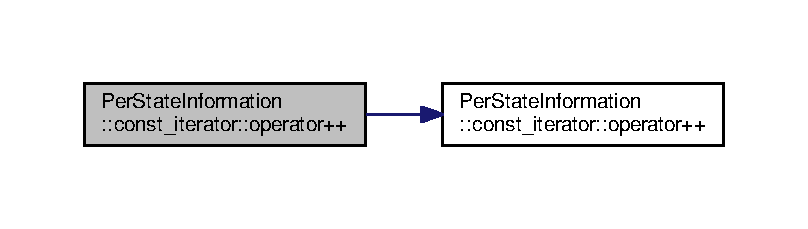
\includegraphics[width=350pt]{classPerStateInformation_1_1const__iterator_a07fb0708c40615406279fb7ca382f698_cgraph}
\end{center}
\end{figure}


\hypertarget{classPerStateInformation_1_1const__iterator_ae2fa5a43e634d0036e97424bad5c1f18}{\index{Per\-State\-Information\-::const\-\_\-iterator@{Per\-State\-Information\-::const\-\_\-iterator}!operator-\/$>$@{operator-\/$>$}}
\index{operator-\/$>$@{operator-\/$>$}!PerStateInformation::const_iterator@{Per\-State\-Information\-::const\-\_\-iterator}}
\subsubsection[{operator-\/$>$}]{\setlength{\rightskip}{0pt plus 5cm}template$<$class Entry$>$ {\bf State\-I\-D}$\ast$ {\bf Per\-State\-Information}$<$ Entry $>$\-::const\-\_\-iterator\-::operator-\/$>$ (
\begin{DoxyParamCaption}
{}
\end{DoxyParamCaption}
)\hspace{0.3cm}{\ttfamily [inline]}}}\label{classPerStateInformation_1_1const__iterator_ae2fa5a43e634d0036e97424bad5c1f18}
\hypertarget{classPerStateInformation_1_1const__iterator_a9e09cdff82fb1b6b669cd28d6ec8bb14}{\index{Per\-State\-Information\-::const\-\_\-iterator@{Per\-State\-Information\-::const\-\_\-iterator}!operator==@{operator==}}
\index{operator==@{operator==}!PerStateInformation::const_iterator@{Per\-State\-Information\-::const\-\_\-iterator}}
\subsubsection[{operator==}]{\setlength{\rightskip}{0pt plus 5cm}template$<$class Entry$>$ bool {\bf Per\-State\-Information}$<$ Entry $>$\-::const\-\_\-iterator\-::operator== (
\begin{DoxyParamCaption}
\item[{const {\bf const\-\_\-iterator} \&}]{rhs}
\end{DoxyParamCaption}
)\hspace{0.3cm}{\ttfamily [inline]}}}\label{classPerStateInformation_1_1const__iterator_a9e09cdff82fb1b6b669cd28d6ec8bb14}


\subsection{Friends And Related Function Documentation}
\hypertarget{classPerStateInformation_1_1const__iterator_ae69462da21a4e3a3b602a69ebc4738c1}{\index{Per\-State\-Information\-::const\-\_\-iterator@{Per\-State\-Information\-::const\-\_\-iterator}!Per\-State\-Information$<$ Entry $>$@{Per\-State\-Information$<$ Entry $>$}}
\index{Per\-State\-Information$<$ Entry $>$@{Per\-State\-Information$<$ Entry $>$}!PerStateInformation::const_iterator@{Per\-State\-Information\-::const\-\_\-iterator}}
\subsubsection[{Per\-State\-Information$<$ Entry $>$}]{\setlength{\rightskip}{0pt plus 5cm}template$<$class Entry$>$ friend class {\bf Per\-State\-Information}$<$ Entry $>$\hspace{0.3cm}{\ttfamily [friend]}}}\label{classPerStateInformation_1_1const__iterator_ae69462da21a4e3a3b602a69ebc4738c1}


The documentation for this class was generated from the following file\-:\begin{DoxyCompactItemize}
\item 
\hyperlink{per__state__information_8h}{per\-\_\-state\-\_\-information.\-h}\end{DoxyCompactItemize}

\hypertarget{classcea__heuristic_1_1ContextEnhancedAdditiveHeuristic}{\section{cea\-\_\-heuristic\-:\-:Context\-Enhanced\-Additive\-Heuristic Class Reference}
\label{classcea__heuristic_1_1ContextEnhancedAdditiveHeuristic}\index{cea\-\_\-heuristic\-::\-Context\-Enhanced\-Additive\-Heuristic@{cea\-\_\-heuristic\-::\-Context\-Enhanced\-Additive\-Heuristic}}
}


{\ttfamily \#include $<$cea\-\_\-heuristic.\-h$>$}



Inheritance diagram for cea\-\_\-heuristic\-:\-:Context\-Enhanced\-Additive\-Heuristic\-:
\nopagebreak
\begin{figure}[H]
\begin{center}
\leavevmode
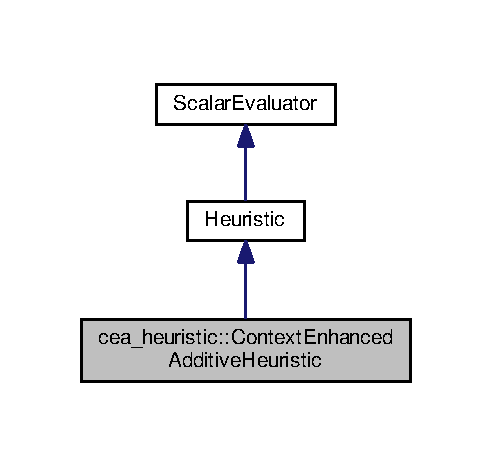
\includegraphics[width=236pt]{classcea__heuristic_1_1ContextEnhancedAdditiveHeuristic__inherit__graph}
\end{center}
\end{figure}


Collaboration diagram for cea\-\_\-heuristic\-:\-:Context\-Enhanced\-Additive\-Heuristic\-:
\nopagebreak
\begin{figure}[H]
\begin{center}
\leavevmode
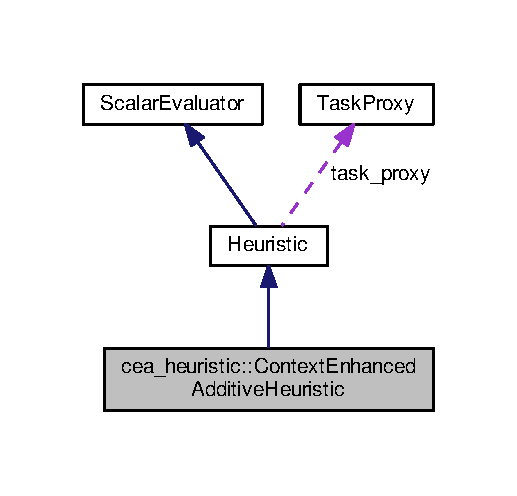
\includegraphics[width=248pt]{classcea__heuristic_1_1ContextEnhancedAdditiveHeuristic__coll__graph}
\end{center}
\end{figure}
\subsection*{Public Member Functions}
\begin{DoxyCompactItemize}
\item 
\hyperlink{classcea__heuristic_1_1ContextEnhancedAdditiveHeuristic_ac062acf8a0b3a904752420bdd02be18b}{Context\-Enhanced\-Additive\-Heuristic} (const \hyperlink{classOptions}{Options} \&opts)
\item 
\hyperlink{classcea__heuristic_1_1ContextEnhancedAdditiveHeuristic_a9e6acd10125851efb6f9e9ae6b9be342}{$\sim$\-Context\-Enhanced\-Additive\-Heuristic} ()
\item 
virtual bool \hyperlink{classcea__heuristic_1_1ContextEnhancedAdditiveHeuristic_a084c0b970b564a8985a9fa8b547de1c8}{dead\-\_\-ends\-\_\-are\-\_\-reliable} () const 
\end{DoxyCompactItemize}
\subsection*{Protected Member Functions}
\begin{DoxyCompactItemize}
\item 
virtual void \hyperlink{classcea__heuristic_1_1ContextEnhancedAdditiveHeuristic_a2c354c358f314bb32ec020f0d9c8bcac}{initialize} ()
\item 
virtual int \hyperlink{classcea__heuristic_1_1ContextEnhancedAdditiveHeuristic_a6071c4aa48d00eb35fdae3f4ed611470}{compute\-\_\-heuristic} (const \hyperlink{classGlobalState}{Global\-State} \&state)
\end{DoxyCompactItemize}
\subsection*{Additional Inherited Members}


\subsection{Constructor \& Destructor Documentation}
\hypertarget{classcea__heuristic_1_1ContextEnhancedAdditiveHeuristic_ac062acf8a0b3a904752420bdd02be18b}{\index{cea\-\_\-heuristic\-::\-Context\-Enhanced\-Additive\-Heuristic@{cea\-\_\-heuristic\-::\-Context\-Enhanced\-Additive\-Heuristic}!Context\-Enhanced\-Additive\-Heuristic@{Context\-Enhanced\-Additive\-Heuristic}}
\index{Context\-Enhanced\-Additive\-Heuristic@{Context\-Enhanced\-Additive\-Heuristic}!cea_heuristic::ContextEnhancedAdditiveHeuristic@{cea\-\_\-heuristic\-::\-Context\-Enhanced\-Additive\-Heuristic}}
\subsubsection[{Context\-Enhanced\-Additive\-Heuristic}]{\setlength{\rightskip}{0pt plus 5cm}cea\-\_\-heuristic\-::\-Context\-Enhanced\-Additive\-Heuristic\-::\-Context\-Enhanced\-Additive\-Heuristic (
\begin{DoxyParamCaption}
\item[{const {\bf Options} \&}]{opts}
\end{DoxyParamCaption}
)}}\label{classcea__heuristic_1_1ContextEnhancedAdditiveHeuristic_ac062acf8a0b3a904752420bdd02be18b}
\hypertarget{classcea__heuristic_1_1ContextEnhancedAdditiveHeuristic_a9e6acd10125851efb6f9e9ae6b9be342}{\index{cea\-\_\-heuristic\-::\-Context\-Enhanced\-Additive\-Heuristic@{cea\-\_\-heuristic\-::\-Context\-Enhanced\-Additive\-Heuristic}!$\sim$\-Context\-Enhanced\-Additive\-Heuristic@{$\sim$\-Context\-Enhanced\-Additive\-Heuristic}}
\index{$\sim$\-Context\-Enhanced\-Additive\-Heuristic@{$\sim$\-Context\-Enhanced\-Additive\-Heuristic}!cea_heuristic::ContextEnhancedAdditiveHeuristic@{cea\-\_\-heuristic\-::\-Context\-Enhanced\-Additive\-Heuristic}}
\subsubsection[{$\sim$\-Context\-Enhanced\-Additive\-Heuristic}]{\setlength{\rightskip}{0pt plus 5cm}cea\-\_\-heuristic\-::\-Context\-Enhanced\-Additive\-Heuristic\-::$\sim$\-Context\-Enhanced\-Additive\-Heuristic (
\begin{DoxyParamCaption}
{}
\end{DoxyParamCaption}
)}}\label{classcea__heuristic_1_1ContextEnhancedAdditiveHeuristic_a9e6acd10125851efb6f9e9ae6b9be342}


\subsection{Member Function Documentation}
\hypertarget{classcea__heuristic_1_1ContextEnhancedAdditiveHeuristic_a6071c4aa48d00eb35fdae3f4ed611470}{\index{cea\-\_\-heuristic\-::\-Context\-Enhanced\-Additive\-Heuristic@{cea\-\_\-heuristic\-::\-Context\-Enhanced\-Additive\-Heuristic}!compute\-\_\-heuristic@{compute\-\_\-heuristic}}
\index{compute\-\_\-heuristic@{compute\-\_\-heuristic}!cea_heuristic::ContextEnhancedAdditiveHeuristic@{cea\-\_\-heuristic\-::\-Context\-Enhanced\-Additive\-Heuristic}}
\subsubsection[{compute\-\_\-heuristic}]{\setlength{\rightskip}{0pt plus 5cm}int cea\-\_\-heuristic\-::\-Context\-Enhanced\-Additive\-Heuristic\-::compute\-\_\-heuristic (
\begin{DoxyParamCaption}
\item[{const {\bf Global\-State} \&}]{state}
\end{DoxyParamCaption}
)\hspace{0.3cm}{\ttfamily [protected]}, {\ttfamily [virtual]}}}\label{classcea__heuristic_1_1ContextEnhancedAdditiveHeuristic_a6071c4aa48d00eb35fdae3f4ed611470}


Implements \hyperlink{classHeuristic_a4fd4e087281805e0e76a814e06d4e506}{Heuristic}.

\hypertarget{classcea__heuristic_1_1ContextEnhancedAdditiveHeuristic_a084c0b970b564a8985a9fa8b547de1c8}{\index{cea\-\_\-heuristic\-::\-Context\-Enhanced\-Additive\-Heuristic@{cea\-\_\-heuristic\-::\-Context\-Enhanced\-Additive\-Heuristic}!dead\-\_\-ends\-\_\-are\-\_\-reliable@{dead\-\_\-ends\-\_\-are\-\_\-reliable}}
\index{dead\-\_\-ends\-\_\-are\-\_\-reliable@{dead\-\_\-ends\-\_\-are\-\_\-reliable}!cea_heuristic::ContextEnhancedAdditiveHeuristic@{cea\-\_\-heuristic\-::\-Context\-Enhanced\-Additive\-Heuristic}}
\subsubsection[{dead\-\_\-ends\-\_\-are\-\_\-reliable}]{\setlength{\rightskip}{0pt plus 5cm}bool cea\-\_\-heuristic\-::\-Context\-Enhanced\-Additive\-Heuristic\-::dead\-\_\-ends\-\_\-are\-\_\-reliable (
\begin{DoxyParamCaption}
{}
\end{DoxyParamCaption}
) const\hspace{0.3cm}{\ttfamily [virtual]}}}\label{classcea__heuristic_1_1ContextEnhancedAdditiveHeuristic_a084c0b970b564a8985a9fa8b547de1c8}


Reimplemented from \hyperlink{classScalarEvaluator_aa4534363976871466aa2be88f82e1a74}{Scalar\-Evaluator}.

\hypertarget{classcea__heuristic_1_1ContextEnhancedAdditiveHeuristic_a2c354c358f314bb32ec020f0d9c8bcac}{\index{cea\-\_\-heuristic\-::\-Context\-Enhanced\-Additive\-Heuristic@{cea\-\_\-heuristic\-::\-Context\-Enhanced\-Additive\-Heuristic}!initialize@{initialize}}
\index{initialize@{initialize}!cea_heuristic::ContextEnhancedAdditiveHeuristic@{cea\-\_\-heuristic\-::\-Context\-Enhanced\-Additive\-Heuristic}}
\subsubsection[{initialize}]{\setlength{\rightskip}{0pt plus 5cm}void cea\-\_\-heuristic\-::\-Context\-Enhanced\-Additive\-Heuristic\-::initialize (
\begin{DoxyParamCaption}
{}
\end{DoxyParamCaption}
)\hspace{0.3cm}{\ttfamily [protected]}, {\ttfamily [virtual]}}}\label{classcea__heuristic_1_1ContextEnhancedAdditiveHeuristic_a2c354c358f314bb32ec020f0d9c8bcac}


Reimplemented from \hyperlink{classHeuristic_a26e75bad1d806657c0ed274b4fe72f0a}{Heuristic}.



The documentation for this class was generated from the following files\-:\begin{DoxyCompactItemize}
\item 
\hyperlink{cea__heuristic_8h}{cea\-\_\-heuristic.\-h}\item 
\hyperlink{cea__heuristic_8cc}{cea\-\_\-heuristic.\-cc}\end{DoxyCompactItemize}

\hypertarget{classCostAdaptedTask}{\section{Cost\-Adapted\-Task Class Reference}
\label{classCostAdaptedTask}\index{Cost\-Adapted\-Task@{Cost\-Adapted\-Task}}
}


{\ttfamily \#include $<$cost\-\_\-adapted\-\_\-task.\-h$>$}



Inheritance diagram for Cost\-Adapted\-Task\-:
\nopagebreak
\begin{figure}[H]
\begin{center}
\leavevmode
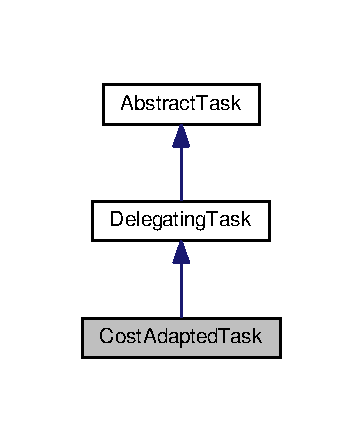
\includegraphics[width=174pt]{classCostAdaptedTask__inherit__graph}
\end{center}
\end{figure}


Collaboration diagram for Cost\-Adapted\-Task\-:
\nopagebreak
\begin{figure}[H]
\begin{center}
\leavevmode
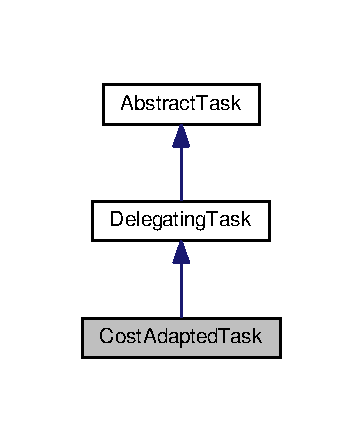
\includegraphics[width=174pt]{classCostAdaptedTask__coll__graph}
\end{center}
\end{figure}
\subsection*{Public Member Functions}
\begin{DoxyCompactItemize}
\item 
\hyperlink{classCostAdaptedTask_af521f614cf302abba45c5c6712fd3686}{Cost\-Adapted\-Task} (const \hyperlink{classOptions}{Options} \&opts)
\item 
virtual \hyperlink{classCostAdaptedTask_a803792c9ebf9f98d0770fc5e6f3d01d7}{$\sim$\-Cost\-Adapted\-Task} () override=default
\item 
virtual int \hyperlink{classCostAdaptedTask_a931aa2a13aaff9410582e903f5cfbc9d}{get\-\_\-operator\-\_\-cost} (int index, bool is\-\_\-axiom) const override
\end{DoxyCompactItemize}
\subsection*{Additional Inherited Members}


\subsection{Constructor \& Destructor Documentation}
\hypertarget{classCostAdaptedTask_af521f614cf302abba45c5c6712fd3686}{\index{Cost\-Adapted\-Task@{Cost\-Adapted\-Task}!Cost\-Adapted\-Task@{Cost\-Adapted\-Task}}
\index{Cost\-Adapted\-Task@{Cost\-Adapted\-Task}!CostAdaptedTask@{Cost\-Adapted\-Task}}
\subsubsection[{Cost\-Adapted\-Task}]{\setlength{\rightskip}{0pt plus 5cm}Cost\-Adapted\-Task\-::\-Cost\-Adapted\-Task (
\begin{DoxyParamCaption}
\item[{const {\bf Options} \&}]{opts}
\end{DoxyParamCaption}
)\hspace{0.3cm}{\ttfamily [explicit]}}}\label{classCostAdaptedTask_af521f614cf302abba45c5c6712fd3686}
\hypertarget{classCostAdaptedTask_a803792c9ebf9f98d0770fc5e6f3d01d7}{\index{Cost\-Adapted\-Task@{Cost\-Adapted\-Task}!$\sim$\-Cost\-Adapted\-Task@{$\sim$\-Cost\-Adapted\-Task}}
\index{$\sim$\-Cost\-Adapted\-Task@{$\sim$\-Cost\-Adapted\-Task}!CostAdaptedTask@{Cost\-Adapted\-Task}}
\subsubsection[{$\sim$\-Cost\-Adapted\-Task}]{\setlength{\rightskip}{0pt plus 5cm}virtual Cost\-Adapted\-Task\-::$\sim$\-Cost\-Adapted\-Task (
\begin{DoxyParamCaption}
{}
\end{DoxyParamCaption}
)\hspace{0.3cm}{\ttfamily [override]}, {\ttfamily [virtual]}, {\ttfamily [default]}}}\label{classCostAdaptedTask_a803792c9ebf9f98d0770fc5e6f3d01d7}


\subsection{Member Function Documentation}
\hypertarget{classCostAdaptedTask_a931aa2a13aaff9410582e903f5cfbc9d}{\index{Cost\-Adapted\-Task@{Cost\-Adapted\-Task}!get\-\_\-operator\-\_\-cost@{get\-\_\-operator\-\_\-cost}}
\index{get\-\_\-operator\-\_\-cost@{get\-\_\-operator\-\_\-cost}!CostAdaptedTask@{Cost\-Adapted\-Task}}
\subsubsection[{get\-\_\-operator\-\_\-cost}]{\setlength{\rightskip}{0pt plus 5cm}int Cost\-Adapted\-Task\-::get\-\_\-operator\-\_\-cost (
\begin{DoxyParamCaption}
\item[{int}]{index, }
\item[{bool}]{is\-\_\-axiom}
\end{DoxyParamCaption}
) const\hspace{0.3cm}{\ttfamily [override]}, {\ttfamily [virtual]}}}\label{classCostAdaptedTask_a931aa2a13aaff9410582e903f5cfbc9d}


Reimplemented from \hyperlink{classDelegatingTask_a88352a7f751b06d0bd5302388d7ec377}{Delegating\-Task}.



Here is the call graph for this function\-:
\nopagebreak
\begin{figure}[H]
\begin{center}
\leavevmode
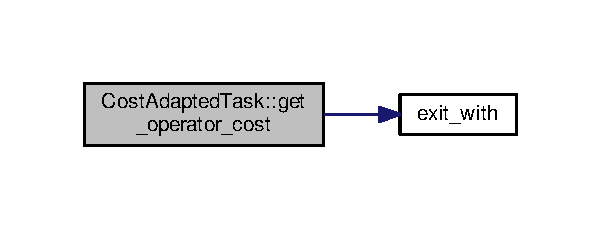
\includegraphics[width=288pt]{classCostAdaptedTask_a931aa2a13aaff9410582e903f5cfbc9d_cgraph}
\end{center}
\end{figure}




The documentation for this class was generated from the following files\-:\begin{DoxyCompactItemize}
\item 
\hyperlink{cost__adapted__task_8h}{cost\-\_\-adapted\-\_\-task.\-h}\item 
\hyperlink{cost__adapted__task_8cc}{cost\-\_\-adapted\-\_\-task.\-cc}\end{DoxyCompactItemize}

\hypertarget{classCountdownTimer}{\section{Countdown\-Timer Class Reference}
\label{classCountdownTimer}\index{Countdown\-Timer@{Countdown\-Timer}}
}


{\ttfamily \#include $<$countdown\-\_\-timer.\-h$>$}

\subsection*{Public Member Functions}
\begin{DoxyCompactItemize}
\item 
\hyperlink{classCountdownTimer_a2fe33274e8b0613547e74fcbb182db0e}{Countdown\-Timer} (double max\-\_\-time)
\item 
\hyperlink{classCountdownTimer_a1cd608b370250db65416ce824e2ad092}{$\sim$\-Countdown\-Timer} ()
\item 
bool \hyperlink{classCountdownTimer_a11351f52bb11757af4264f59c1f6c144}{is\-\_\-expired} () const 
\end{DoxyCompactItemize}
\subsection*{Friends}
\begin{DoxyCompactItemize}
\item 
std\-::ostream \& \hyperlink{classCountdownTimer_a2407f49edc80534d80cb2bd37a74eae9}{operator$<$$<$} (std\-::ostream \&os, const \hyperlink{classCountdownTimer}{Countdown\-Timer} \&cd\-\_\-timer)
\end{DoxyCompactItemize}


\subsection{Constructor \& Destructor Documentation}
\hypertarget{classCountdownTimer_a2fe33274e8b0613547e74fcbb182db0e}{\index{Countdown\-Timer@{Countdown\-Timer}!Countdown\-Timer@{Countdown\-Timer}}
\index{Countdown\-Timer@{Countdown\-Timer}!CountdownTimer@{Countdown\-Timer}}
\subsubsection[{Countdown\-Timer}]{\setlength{\rightskip}{0pt plus 5cm}Countdown\-Timer\-::\-Countdown\-Timer (
\begin{DoxyParamCaption}
\item[{double}]{max\-\_\-time}
\end{DoxyParamCaption}
)\hspace{0.3cm}{\ttfamily [explicit]}}}\label{classCountdownTimer_a2fe33274e8b0613547e74fcbb182db0e}
\hypertarget{classCountdownTimer_a1cd608b370250db65416ce824e2ad092}{\index{Countdown\-Timer@{Countdown\-Timer}!$\sim$\-Countdown\-Timer@{$\sim$\-Countdown\-Timer}}
\index{$\sim$\-Countdown\-Timer@{$\sim$\-Countdown\-Timer}!CountdownTimer@{Countdown\-Timer}}
\subsubsection[{$\sim$\-Countdown\-Timer}]{\setlength{\rightskip}{0pt plus 5cm}Countdown\-Timer\-::$\sim$\-Countdown\-Timer (
\begin{DoxyParamCaption}
{}
\end{DoxyParamCaption}
)}}\label{classCountdownTimer_a1cd608b370250db65416ce824e2ad092}


\subsection{Member Function Documentation}
\hypertarget{classCountdownTimer_a11351f52bb11757af4264f59c1f6c144}{\index{Countdown\-Timer@{Countdown\-Timer}!is\-\_\-expired@{is\-\_\-expired}}
\index{is\-\_\-expired@{is\-\_\-expired}!CountdownTimer@{Countdown\-Timer}}
\subsubsection[{is\-\_\-expired}]{\setlength{\rightskip}{0pt plus 5cm}bool Countdown\-Timer\-::is\-\_\-expired (
\begin{DoxyParamCaption}
{}
\end{DoxyParamCaption}
) const}}\label{classCountdownTimer_a11351f52bb11757af4264f59c1f6c144}


\subsection{Friends And Related Function Documentation}
\hypertarget{classCountdownTimer_a2407f49edc80534d80cb2bd37a74eae9}{\index{Countdown\-Timer@{Countdown\-Timer}!operator$<$$<$@{operator$<$$<$}}
\index{operator$<$$<$@{operator$<$$<$}!CountdownTimer@{Countdown\-Timer}}
\subsubsection[{operator$<$$<$}]{\setlength{\rightskip}{0pt plus 5cm}std\-::ostream\& operator$<$$<$ (
\begin{DoxyParamCaption}
\item[{std\-::ostream \&}]{os, }
\item[{const {\bf Countdown\-Timer} \&}]{cd\-\_\-timer}
\end{DoxyParamCaption}
)\hspace{0.3cm}{\ttfamily [friend]}}}\label{classCountdownTimer_a2407f49edc80534d80cb2bd37a74eae9}


The documentation for this class was generated from the following files\-:\begin{DoxyCompactItemize}
\item 
\hyperlink{countdown__timer_8h}{countdown\-\_\-timer.\-h}\item 
\hyperlink{countdown__timer_8cc}{countdown\-\_\-timer.\-cc}\end{DoxyCompactItemize}

\hypertarget{classDelegatingTask}{\section{Delegating\-Task Class Reference}
\label{classDelegatingTask}\index{Delegating\-Task@{Delegating\-Task}}
}


{\ttfamily \#include $<$delegating\-\_\-task.\-h$>$}



Inheritance diagram for Delegating\-Task\-:
\nopagebreak
\begin{figure}[H]
\begin{center}
\leavevmode
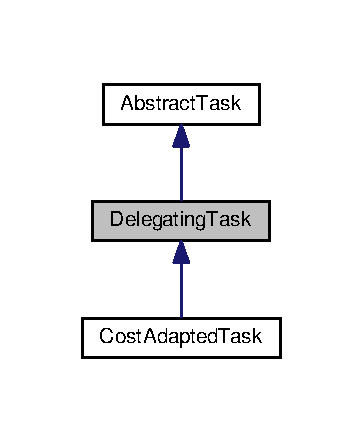
\includegraphics[width=174pt]{classDelegatingTask__inherit__graph}
\end{center}
\end{figure}


Collaboration diagram for Delegating\-Task\-:
\nopagebreak
\begin{figure}[H]
\begin{center}
\leavevmode
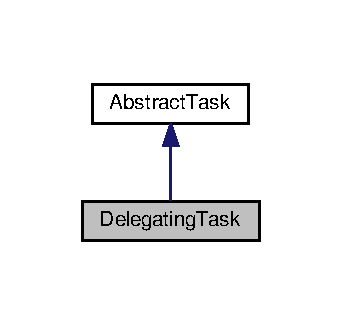
\includegraphics[width=164pt]{classDelegatingTask__coll__graph}
\end{center}
\end{figure}
\subsection*{Public Member Functions}
\begin{DoxyCompactItemize}
\item 
\hyperlink{classDelegatingTask_a80da8ef8d04dc5c69ede77d0e2c0601f}{Delegating\-Task} (const std\-::shared\-\_\-ptr$<$ \hyperlink{classAbstractTask}{Abstract\-Task} $>$ \hyperlink{classDelegatingTask_a333f326a36598317987befd345c7836e}{parent})
\item 
virtual \hyperlink{classDelegatingTask_af06a332e2641b91d0de7e17baa00e103}{$\sim$\-Delegating\-Task} () override=default
\item 
virtual int \hyperlink{classDelegatingTask_a1b3289d0d7b5567e38e06350788c1ece}{get\-\_\-num\-\_\-variables} () const override
\item 
virtual const std\-::string \& \hyperlink{classDelegatingTask_a6d0d9b3cfb2eac8f46dbbcbb2284dab3}{get\-\_\-variable\-\_\-name} (int var) const override
\item 
virtual int \hyperlink{classDelegatingTask_a2744ecccb1f245e7d2197e353d79e632}{get\-\_\-variable\-\_\-domain\-\_\-size} (int var) const override
\item 
virtual const std\-::string \& \hyperlink{classDelegatingTask_aff6c956a3c936fcfeac368388e75c385}{get\-\_\-fact\-\_\-name} (int var, int value) const override
\item 
virtual int \hyperlink{classDelegatingTask_a88352a7f751b06d0bd5302388d7ec377}{get\-\_\-operator\-\_\-cost} (int index, bool is\-\_\-axiom) const override
\item 
virtual const std\-::string \& \hyperlink{classDelegatingTask_af0069346a9bf01c82e6ca9f5220f0f1d}{get\-\_\-operator\-\_\-name} (int index, bool is\-\_\-axiom) const override
\item 
virtual int \hyperlink{classDelegatingTask_a17d94e5b76add2569236c252ede36180}{get\-\_\-num\-\_\-operators} () const override
\item 
virtual int \hyperlink{classDelegatingTask_a1b2ae69912faf4c5f58a13bd3f744dec}{get\-\_\-num\-\_\-operator\-\_\-preconditions} (int index, bool is\-\_\-axiom) const override
\item 
virtual std\-::pair$<$ int, int $>$ \hyperlink{classDelegatingTask_a20b4112f42c5cabdb2b578db176b0d1f}{get\-\_\-operator\-\_\-precondition} (int op\-\_\-index, int fact\-\_\-index, bool is\-\_\-axiom) const override
\item 
virtual int \hyperlink{classDelegatingTask_af3f485cdbd1872e11ca53a47da104d35}{get\-\_\-num\-\_\-operator\-\_\-effects} (int op\-\_\-index, bool is\-\_\-axiom) const override
\item 
virtual int \hyperlink{classDelegatingTask_a63119dfe36f38c8eaefa093a8d944b70}{get\-\_\-num\-\_\-operator\-\_\-effect\-\_\-conditions} (int op\-\_\-index, int eff\-\_\-index, bool is\-\_\-axiom) const override
\item 
virtual std\-::pair$<$ int, int $>$ \hyperlink{classDelegatingTask_aaabb1108e7759110b1125482ba528e74}{get\-\_\-operator\-\_\-effect\-\_\-condition} (int op\-\_\-index, int eff\-\_\-index, int cond\-\_\-index, bool is\-\_\-axiom) const override
\item 
virtual std\-::pair$<$ int, int $>$ \hyperlink{classDelegatingTask_a3f2571a63c2b22327df586e5a9d0df3e}{get\-\_\-operator\-\_\-effect} (int op\-\_\-index, int eff\-\_\-index, bool is\-\_\-axiom) const override
\item 
virtual const \hyperlink{classGlobalOperator}{Global\-Operator} $\ast$ \hyperlink{classDelegatingTask_a3807759260be9458378190ff25751b70}{get\-\_\-global\-\_\-operator} (int index, bool is\-\_\-axiom) const override
\item 
virtual int \hyperlink{classDelegatingTask_af215094028d4c83cce4321e2cb2d011b}{get\-\_\-num\-\_\-axioms} () const override
\item 
virtual int \hyperlink{classDelegatingTask_a25fcb2255c42d684f89524de475f166e}{get\-\_\-num\-\_\-goals} () const override
\item 
virtual std\-::pair$<$ int, int $>$ \hyperlink{classDelegatingTask_a41ec9662ab3cd04af01e64a3805436fc}{get\-\_\-goal\-\_\-fact} (int index) const override
\item 
virtual std\-::vector$<$ int $>$ \hyperlink{classDelegatingTask_a62c81bb064e4d5e72f619f01e1e3f73c}{get\-\_\-initial\-\_\-state\-\_\-values} () const override
\item 
virtual std\-::vector$<$ int $>$ \hyperlink{classDelegatingTask_a04ac3437f7f4ae171190ef5972d8d16e}{get\-\_\-state\-\_\-values} (const \hyperlink{classGlobalState}{Global\-State} \&global\-\_\-state) const override
\end{DoxyCompactItemize}
\subsection*{Protected Attributes}
\begin{DoxyCompactItemize}
\item 
const std\-::shared\-\_\-ptr\\*
$<$ \hyperlink{classAbstractTask}{Abstract\-Task} $>$ \hyperlink{classDelegatingTask_a333f326a36598317987befd345c7836e}{parent}
\end{DoxyCompactItemize}


\subsection{Constructor \& Destructor Documentation}
\hypertarget{classDelegatingTask_a80da8ef8d04dc5c69ede77d0e2c0601f}{\index{Delegating\-Task@{Delegating\-Task}!Delegating\-Task@{Delegating\-Task}}
\index{Delegating\-Task@{Delegating\-Task}!DelegatingTask@{Delegating\-Task}}
\subsubsection[{Delegating\-Task}]{\setlength{\rightskip}{0pt plus 5cm}Delegating\-Task\-::\-Delegating\-Task (
\begin{DoxyParamCaption}
\item[{const std\-::shared\-\_\-ptr$<$ {\bf Abstract\-Task} $>$}]{parent}
\end{DoxyParamCaption}
)\hspace{0.3cm}{\ttfamily [explicit]}}}\label{classDelegatingTask_a80da8ef8d04dc5c69ede77d0e2c0601f}
\hypertarget{classDelegatingTask_af06a332e2641b91d0de7e17baa00e103}{\index{Delegating\-Task@{Delegating\-Task}!$\sim$\-Delegating\-Task@{$\sim$\-Delegating\-Task}}
\index{$\sim$\-Delegating\-Task@{$\sim$\-Delegating\-Task}!DelegatingTask@{Delegating\-Task}}
\subsubsection[{$\sim$\-Delegating\-Task}]{\setlength{\rightskip}{0pt plus 5cm}virtual Delegating\-Task\-::$\sim$\-Delegating\-Task (
\begin{DoxyParamCaption}
{}
\end{DoxyParamCaption}
)\hspace{0.3cm}{\ttfamily [override]}, {\ttfamily [virtual]}, {\ttfamily [default]}}}\label{classDelegatingTask_af06a332e2641b91d0de7e17baa00e103}


\subsection{Member Function Documentation}
\hypertarget{classDelegatingTask_aff6c956a3c936fcfeac368388e75c385}{\index{Delegating\-Task@{Delegating\-Task}!get\-\_\-fact\-\_\-name@{get\-\_\-fact\-\_\-name}}
\index{get\-\_\-fact\-\_\-name@{get\-\_\-fact\-\_\-name}!DelegatingTask@{Delegating\-Task}}
\subsubsection[{get\-\_\-fact\-\_\-name}]{\setlength{\rightskip}{0pt plus 5cm}const string \& Delegating\-Task\-::get\-\_\-fact\-\_\-name (
\begin{DoxyParamCaption}
\item[{int}]{var, }
\item[{int}]{value}
\end{DoxyParamCaption}
) const\hspace{0.3cm}{\ttfamily [override]}, {\ttfamily [virtual]}}}\label{classDelegatingTask_aff6c956a3c936fcfeac368388e75c385}


Implements \hyperlink{classAbstractTask_a8ad9d3e97f1aa8fcde6cbc7844609c79}{Abstract\-Task}.

\hypertarget{classDelegatingTask_a3807759260be9458378190ff25751b70}{\index{Delegating\-Task@{Delegating\-Task}!get\-\_\-global\-\_\-operator@{get\-\_\-global\-\_\-operator}}
\index{get\-\_\-global\-\_\-operator@{get\-\_\-global\-\_\-operator}!DelegatingTask@{Delegating\-Task}}
\subsubsection[{get\-\_\-global\-\_\-operator}]{\setlength{\rightskip}{0pt plus 5cm}const {\bf Global\-Operator} $\ast$ Delegating\-Task\-::get\-\_\-global\-\_\-operator (
\begin{DoxyParamCaption}
\item[{int}]{index, }
\item[{bool}]{is\-\_\-axiom}
\end{DoxyParamCaption}
) const\hspace{0.3cm}{\ttfamily [override]}, {\ttfamily [virtual]}}}\label{classDelegatingTask_a3807759260be9458378190ff25751b70}


Implements \hyperlink{classAbstractTask_ad0335ea9f89fa54b846780b55fad2545}{Abstract\-Task}.

\hypertarget{classDelegatingTask_a41ec9662ab3cd04af01e64a3805436fc}{\index{Delegating\-Task@{Delegating\-Task}!get\-\_\-goal\-\_\-fact@{get\-\_\-goal\-\_\-fact}}
\index{get\-\_\-goal\-\_\-fact@{get\-\_\-goal\-\_\-fact}!DelegatingTask@{Delegating\-Task}}
\subsubsection[{get\-\_\-goal\-\_\-fact}]{\setlength{\rightskip}{0pt plus 5cm}pair$<$ int, int $>$ Delegating\-Task\-::get\-\_\-goal\-\_\-fact (
\begin{DoxyParamCaption}
\item[{int}]{index}
\end{DoxyParamCaption}
) const\hspace{0.3cm}{\ttfamily [override]}, {\ttfamily [virtual]}}}\label{classDelegatingTask_a41ec9662ab3cd04af01e64a3805436fc}


Implements \hyperlink{classAbstractTask_a737c7aca71dbf64b673236a0af4d8dde}{Abstract\-Task}.

\hypertarget{classDelegatingTask_a62c81bb064e4d5e72f619f01e1e3f73c}{\index{Delegating\-Task@{Delegating\-Task}!get\-\_\-initial\-\_\-state\-\_\-values@{get\-\_\-initial\-\_\-state\-\_\-values}}
\index{get\-\_\-initial\-\_\-state\-\_\-values@{get\-\_\-initial\-\_\-state\-\_\-values}!DelegatingTask@{Delegating\-Task}}
\subsubsection[{get\-\_\-initial\-\_\-state\-\_\-values}]{\setlength{\rightskip}{0pt plus 5cm}std\-::vector$<$ int $>$ Delegating\-Task\-::get\-\_\-initial\-\_\-state\-\_\-values (
\begin{DoxyParamCaption}
{}
\end{DoxyParamCaption}
) const\hspace{0.3cm}{\ttfamily [override]}, {\ttfamily [virtual]}}}\label{classDelegatingTask_a62c81bb064e4d5e72f619f01e1e3f73c}


Implements \hyperlink{classAbstractTask_a9de0ce6fb5349cc114cef522c54c595e}{Abstract\-Task}.

\hypertarget{classDelegatingTask_af215094028d4c83cce4321e2cb2d011b}{\index{Delegating\-Task@{Delegating\-Task}!get\-\_\-num\-\_\-axioms@{get\-\_\-num\-\_\-axioms}}
\index{get\-\_\-num\-\_\-axioms@{get\-\_\-num\-\_\-axioms}!DelegatingTask@{Delegating\-Task}}
\subsubsection[{get\-\_\-num\-\_\-axioms}]{\setlength{\rightskip}{0pt plus 5cm}int Delegating\-Task\-::get\-\_\-num\-\_\-axioms (
\begin{DoxyParamCaption}
{}
\end{DoxyParamCaption}
) const\hspace{0.3cm}{\ttfamily [override]}, {\ttfamily [virtual]}}}\label{classDelegatingTask_af215094028d4c83cce4321e2cb2d011b}


Implements \hyperlink{classAbstractTask_a0e713664080d2a70036b6307779e7593}{Abstract\-Task}.

\hypertarget{classDelegatingTask_a25fcb2255c42d684f89524de475f166e}{\index{Delegating\-Task@{Delegating\-Task}!get\-\_\-num\-\_\-goals@{get\-\_\-num\-\_\-goals}}
\index{get\-\_\-num\-\_\-goals@{get\-\_\-num\-\_\-goals}!DelegatingTask@{Delegating\-Task}}
\subsubsection[{get\-\_\-num\-\_\-goals}]{\setlength{\rightskip}{0pt plus 5cm}int Delegating\-Task\-::get\-\_\-num\-\_\-goals (
\begin{DoxyParamCaption}
{}
\end{DoxyParamCaption}
) const\hspace{0.3cm}{\ttfamily [override]}, {\ttfamily [virtual]}}}\label{classDelegatingTask_a25fcb2255c42d684f89524de475f166e}


Implements \hyperlink{classAbstractTask_a4e8335bdbfad228faf76e3c085d2ae4a}{Abstract\-Task}.

\hypertarget{classDelegatingTask_a63119dfe36f38c8eaefa093a8d944b70}{\index{Delegating\-Task@{Delegating\-Task}!get\-\_\-num\-\_\-operator\-\_\-effect\-\_\-conditions@{get\-\_\-num\-\_\-operator\-\_\-effect\-\_\-conditions}}
\index{get\-\_\-num\-\_\-operator\-\_\-effect\-\_\-conditions@{get\-\_\-num\-\_\-operator\-\_\-effect\-\_\-conditions}!DelegatingTask@{Delegating\-Task}}
\subsubsection[{get\-\_\-num\-\_\-operator\-\_\-effect\-\_\-conditions}]{\setlength{\rightskip}{0pt plus 5cm}int Delegating\-Task\-::get\-\_\-num\-\_\-operator\-\_\-effect\-\_\-conditions (
\begin{DoxyParamCaption}
\item[{int}]{op\-\_\-index, }
\item[{int}]{eff\-\_\-index, }
\item[{bool}]{is\-\_\-axiom}
\end{DoxyParamCaption}
) const\hspace{0.3cm}{\ttfamily [override]}, {\ttfamily [virtual]}}}\label{classDelegatingTask_a63119dfe36f38c8eaefa093a8d944b70}


Implements \hyperlink{classAbstractTask_a41642ad827682428ba1c099ecbde18ae}{Abstract\-Task}.

\hypertarget{classDelegatingTask_af3f485cdbd1872e11ca53a47da104d35}{\index{Delegating\-Task@{Delegating\-Task}!get\-\_\-num\-\_\-operator\-\_\-effects@{get\-\_\-num\-\_\-operator\-\_\-effects}}
\index{get\-\_\-num\-\_\-operator\-\_\-effects@{get\-\_\-num\-\_\-operator\-\_\-effects}!DelegatingTask@{Delegating\-Task}}
\subsubsection[{get\-\_\-num\-\_\-operator\-\_\-effects}]{\setlength{\rightskip}{0pt plus 5cm}int Delegating\-Task\-::get\-\_\-num\-\_\-operator\-\_\-effects (
\begin{DoxyParamCaption}
\item[{int}]{op\-\_\-index, }
\item[{bool}]{is\-\_\-axiom}
\end{DoxyParamCaption}
) const\hspace{0.3cm}{\ttfamily [override]}, {\ttfamily [virtual]}}}\label{classDelegatingTask_af3f485cdbd1872e11ca53a47da104d35}


Implements \hyperlink{classAbstractTask_a101be8c121199154315a3539e59796b2}{Abstract\-Task}.

\hypertarget{classDelegatingTask_a1b2ae69912faf4c5f58a13bd3f744dec}{\index{Delegating\-Task@{Delegating\-Task}!get\-\_\-num\-\_\-operator\-\_\-preconditions@{get\-\_\-num\-\_\-operator\-\_\-preconditions}}
\index{get\-\_\-num\-\_\-operator\-\_\-preconditions@{get\-\_\-num\-\_\-operator\-\_\-preconditions}!DelegatingTask@{Delegating\-Task}}
\subsubsection[{get\-\_\-num\-\_\-operator\-\_\-preconditions}]{\setlength{\rightskip}{0pt plus 5cm}int Delegating\-Task\-::get\-\_\-num\-\_\-operator\-\_\-preconditions (
\begin{DoxyParamCaption}
\item[{int}]{index, }
\item[{bool}]{is\-\_\-axiom}
\end{DoxyParamCaption}
) const\hspace{0.3cm}{\ttfamily [override]}, {\ttfamily [virtual]}}}\label{classDelegatingTask_a1b2ae69912faf4c5f58a13bd3f744dec}


Implements \hyperlink{classAbstractTask_a2913e3d94adf9ce73ecf93a76efd64c0}{Abstract\-Task}.

\hypertarget{classDelegatingTask_a17d94e5b76add2569236c252ede36180}{\index{Delegating\-Task@{Delegating\-Task}!get\-\_\-num\-\_\-operators@{get\-\_\-num\-\_\-operators}}
\index{get\-\_\-num\-\_\-operators@{get\-\_\-num\-\_\-operators}!DelegatingTask@{Delegating\-Task}}
\subsubsection[{get\-\_\-num\-\_\-operators}]{\setlength{\rightskip}{0pt plus 5cm}int Delegating\-Task\-::get\-\_\-num\-\_\-operators (
\begin{DoxyParamCaption}
{}
\end{DoxyParamCaption}
) const\hspace{0.3cm}{\ttfamily [override]}, {\ttfamily [virtual]}}}\label{classDelegatingTask_a17d94e5b76add2569236c252ede36180}


Implements \hyperlink{classAbstractTask_a616388eda808179e2dafcf8030348732}{Abstract\-Task}.

\hypertarget{classDelegatingTask_a1b3289d0d7b5567e38e06350788c1ece}{\index{Delegating\-Task@{Delegating\-Task}!get\-\_\-num\-\_\-variables@{get\-\_\-num\-\_\-variables}}
\index{get\-\_\-num\-\_\-variables@{get\-\_\-num\-\_\-variables}!DelegatingTask@{Delegating\-Task}}
\subsubsection[{get\-\_\-num\-\_\-variables}]{\setlength{\rightskip}{0pt plus 5cm}int Delegating\-Task\-::get\-\_\-num\-\_\-variables (
\begin{DoxyParamCaption}
{}
\end{DoxyParamCaption}
) const\hspace{0.3cm}{\ttfamily [override]}, {\ttfamily [virtual]}}}\label{classDelegatingTask_a1b3289d0d7b5567e38e06350788c1ece}


Implements \hyperlink{classAbstractTask_ab0f878648c015fb918567403e80d4e4b}{Abstract\-Task}.

\hypertarget{classDelegatingTask_a88352a7f751b06d0bd5302388d7ec377}{\index{Delegating\-Task@{Delegating\-Task}!get\-\_\-operator\-\_\-cost@{get\-\_\-operator\-\_\-cost}}
\index{get\-\_\-operator\-\_\-cost@{get\-\_\-operator\-\_\-cost}!DelegatingTask@{Delegating\-Task}}
\subsubsection[{get\-\_\-operator\-\_\-cost}]{\setlength{\rightskip}{0pt plus 5cm}int Delegating\-Task\-::get\-\_\-operator\-\_\-cost (
\begin{DoxyParamCaption}
\item[{int}]{index, }
\item[{bool}]{is\-\_\-axiom}
\end{DoxyParamCaption}
) const\hspace{0.3cm}{\ttfamily [override]}, {\ttfamily [virtual]}}}\label{classDelegatingTask_a88352a7f751b06d0bd5302388d7ec377}


Implements \hyperlink{classAbstractTask_aeeb845c0f21bb3517d2ed79c8fdbf575}{Abstract\-Task}.



Reimplemented in \hyperlink{classCostAdaptedTask_a931aa2a13aaff9410582e903f5cfbc9d}{Cost\-Adapted\-Task}.

\hypertarget{classDelegatingTask_a3f2571a63c2b22327df586e5a9d0df3e}{\index{Delegating\-Task@{Delegating\-Task}!get\-\_\-operator\-\_\-effect@{get\-\_\-operator\-\_\-effect}}
\index{get\-\_\-operator\-\_\-effect@{get\-\_\-operator\-\_\-effect}!DelegatingTask@{Delegating\-Task}}
\subsubsection[{get\-\_\-operator\-\_\-effect}]{\setlength{\rightskip}{0pt plus 5cm}pair$<$ int, int $>$ Delegating\-Task\-::get\-\_\-operator\-\_\-effect (
\begin{DoxyParamCaption}
\item[{int}]{op\-\_\-index, }
\item[{int}]{eff\-\_\-index, }
\item[{bool}]{is\-\_\-axiom}
\end{DoxyParamCaption}
) const\hspace{0.3cm}{\ttfamily [override]}, {\ttfamily [virtual]}}}\label{classDelegatingTask_a3f2571a63c2b22327df586e5a9d0df3e}


Implements \hyperlink{classAbstractTask_a4244a150e31b841e65f72ce89fa6ddad}{Abstract\-Task}.

\hypertarget{classDelegatingTask_aaabb1108e7759110b1125482ba528e74}{\index{Delegating\-Task@{Delegating\-Task}!get\-\_\-operator\-\_\-effect\-\_\-condition@{get\-\_\-operator\-\_\-effect\-\_\-condition}}
\index{get\-\_\-operator\-\_\-effect\-\_\-condition@{get\-\_\-operator\-\_\-effect\-\_\-condition}!DelegatingTask@{Delegating\-Task}}
\subsubsection[{get\-\_\-operator\-\_\-effect\-\_\-condition}]{\setlength{\rightskip}{0pt plus 5cm}pair$<$ int, int $>$ Delegating\-Task\-::get\-\_\-operator\-\_\-effect\-\_\-condition (
\begin{DoxyParamCaption}
\item[{int}]{op\-\_\-index, }
\item[{int}]{eff\-\_\-index, }
\item[{int}]{cond\-\_\-index, }
\item[{bool}]{is\-\_\-axiom}
\end{DoxyParamCaption}
) const\hspace{0.3cm}{\ttfamily [override]}, {\ttfamily [virtual]}}}\label{classDelegatingTask_aaabb1108e7759110b1125482ba528e74}


Implements \hyperlink{classAbstractTask_a08f0a9248a99ccd0a1fdee940e0c0c4e}{Abstract\-Task}.

\hypertarget{classDelegatingTask_af0069346a9bf01c82e6ca9f5220f0f1d}{\index{Delegating\-Task@{Delegating\-Task}!get\-\_\-operator\-\_\-name@{get\-\_\-operator\-\_\-name}}
\index{get\-\_\-operator\-\_\-name@{get\-\_\-operator\-\_\-name}!DelegatingTask@{Delegating\-Task}}
\subsubsection[{get\-\_\-operator\-\_\-name}]{\setlength{\rightskip}{0pt plus 5cm}const string \& Delegating\-Task\-::get\-\_\-operator\-\_\-name (
\begin{DoxyParamCaption}
\item[{int}]{index, }
\item[{bool}]{is\-\_\-axiom}
\end{DoxyParamCaption}
) const\hspace{0.3cm}{\ttfamily [override]}, {\ttfamily [virtual]}}}\label{classDelegatingTask_af0069346a9bf01c82e6ca9f5220f0f1d}


Implements \hyperlink{classAbstractTask_a528cea78d19468e616b2936aba22ea64}{Abstract\-Task}.

\hypertarget{classDelegatingTask_a20b4112f42c5cabdb2b578db176b0d1f}{\index{Delegating\-Task@{Delegating\-Task}!get\-\_\-operator\-\_\-precondition@{get\-\_\-operator\-\_\-precondition}}
\index{get\-\_\-operator\-\_\-precondition@{get\-\_\-operator\-\_\-precondition}!DelegatingTask@{Delegating\-Task}}
\subsubsection[{get\-\_\-operator\-\_\-precondition}]{\setlength{\rightskip}{0pt plus 5cm}pair$<$ int, int $>$ Delegating\-Task\-::get\-\_\-operator\-\_\-precondition (
\begin{DoxyParamCaption}
\item[{int}]{op\-\_\-index, }
\item[{int}]{fact\-\_\-index, }
\item[{bool}]{is\-\_\-axiom}
\end{DoxyParamCaption}
) const\hspace{0.3cm}{\ttfamily [override]}, {\ttfamily [virtual]}}}\label{classDelegatingTask_a20b4112f42c5cabdb2b578db176b0d1f}


Implements \hyperlink{classAbstractTask_a6d089445ffef1e87abdf2f989c275402}{Abstract\-Task}.

\hypertarget{classDelegatingTask_a04ac3437f7f4ae171190ef5972d8d16e}{\index{Delegating\-Task@{Delegating\-Task}!get\-\_\-state\-\_\-values@{get\-\_\-state\-\_\-values}}
\index{get\-\_\-state\-\_\-values@{get\-\_\-state\-\_\-values}!DelegatingTask@{Delegating\-Task}}
\subsubsection[{get\-\_\-state\-\_\-values}]{\setlength{\rightskip}{0pt plus 5cm}vector$<$ int $>$ Delegating\-Task\-::get\-\_\-state\-\_\-values (
\begin{DoxyParamCaption}
\item[{const {\bf Global\-State} \&}]{global\-\_\-state}
\end{DoxyParamCaption}
) const\hspace{0.3cm}{\ttfamily [override]}, {\ttfamily [virtual]}}}\label{classDelegatingTask_a04ac3437f7f4ae171190ef5972d8d16e}


Implements \hyperlink{classAbstractTask_a047d223704b817c72274f42c05fe3c7d}{Abstract\-Task}.

\hypertarget{classDelegatingTask_a2744ecccb1f245e7d2197e353d79e632}{\index{Delegating\-Task@{Delegating\-Task}!get\-\_\-variable\-\_\-domain\-\_\-size@{get\-\_\-variable\-\_\-domain\-\_\-size}}
\index{get\-\_\-variable\-\_\-domain\-\_\-size@{get\-\_\-variable\-\_\-domain\-\_\-size}!DelegatingTask@{Delegating\-Task}}
\subsubsection[{get\-\_\-variable\-\_\-domain\-\_\-size}]{\setlength{\rightskip}{0pt plus 5cm}int Delegating\-Task\-::get\-\_\-variable\-\_\-domain\-\_\-size (
\begin{DoxyParamCaption}
\item[{int}]{var}
\end{DoxyParamCaption}
) const\hspace{0.3cm}{\ttfamily [override]}, {\ttfamily [virtual]}}}\label{classDelegatingTask_a2744ecccb1f245e7d2197e353d79e632}


Implements \hyperlink{classAbstractTask_a8f229a999a431a27c75daad6bb86474e}{Abstract\-Task}.

\hypertarget{classDelegatingTask_a6d0d9b3cfb2eac8f46dbbcbb2284dab3}{\index{Delegating\-Task@{Delegating\-Task}!get\-\_\-variable\-\_\-name@{get\-\_\-variable\-\_\-name}}
\index{get\-\_\-variable\-\_\-name@{get\-\_\-variable\-\_\-name}!DelegatingTask@{Delegating\-Task}}
\subsubsection[{get\-\_\-variable\-\_\-name}]{\setlength{\rightskip}{0pt plus 5cm}const string \& Delegating\-Task\-::get\-\_\-variable\-\_\-name (
\begin{DoxyParamCaption}
\item[{int}]{var}
\end{DoxyParamCaption}
) const\hspace{0.3cm}{\ttfamily [override]}, {\ttfamily [virtual]}}}\label{classDelegatingTask_a6d0d9b3cfb2eac8f46dbbcbb2284dab3}


Implements \hyperlink{classAbstractTask_acf846013bb556a5d5169b13a6bb879a5}{Abstract\-Task}.



\subsection{Member Data Documentation}
\hypertarget{classDelegatingTask_a333f326a36598317987befd345c7836e}{\index{Delegating\-Task@{Delegating\-Task}!parent@{parent}}
\index{parent@{parent}!DelegatingTask@{Delegating\-Task}}
\subsubsection[{parent}]{\setlength{\rightskip}{0pt plus 5cm}const std\-::shared\-\_\-ptr$<${\bf Abstract\-Task}$>$ Delegating\-Task\-::parent\hspace{0.3cm}{\ttfamily [protected]}}}\label{classDelegatingTask_a333f326a36598317987befd345c7836e}


The documentation for this class was generated from the following files\-:\begin{DoxyCompactItemize}
\item 
\hyperlink{delegating__task_8h}{delegating\-\_\-task.\-h}\item 
\hyperlink{delegating__task_8cc}{delegating\-\_\-task.\-cc}\end{DoxyCompactItemize}

\hypertarget{classDocPrinter}{\section{Doc\-Printer Class Reference}
\label{classDocPrinter}\index{Doc\-Printer@{Doc\-Printer}}
}


{\ttfamily \#include $<$option\-\_\-parser\-\_\-util.\-h$>$}



Inheritance diagram for Doc\-Printer\-:
\nopagebreak
\begin{figure}[H]
\begin{center}
\leavevmode
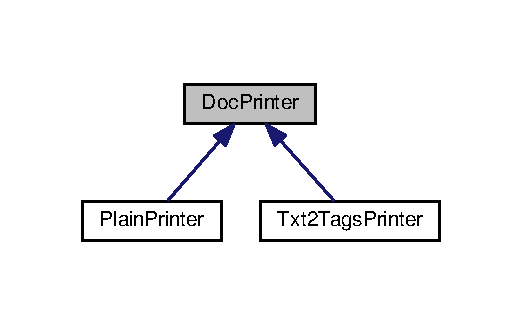
\includegraphics[width=251pt]{classDocPrinter__inherit__graph}
\end{center}
\end{figure}
\subsection*{Public Member Functions}
\begin{DoxyCompactItemize}
\item 
\hyperlink{classDocPrinter_af6d4306e2dc03bc5151adf76e03e1f15}{Doc\-Printer} (std\-::ostream \&out)
\item 
virtual \hyperlink{classDocPrinter_aba059ba132eb4143d2454e30e8bec9c5}{$\sim$\-Doc\-Printer} ()
\item 
virtual void \hyperlink{classDocPrinter_a7da00e32e5758f07b5a1b6cd5d4e9824}{print\-\_\-all} ()
\item 
virtual void \hyperlink{classDocPrinter_a70234bd56a73aa917edf170be8415ce6}{print\-\_\-category} (std\-::string category\-\_\-name)
\item 
virtual void \hyperlink{classDocPrinter_a0253343f6a7ffef9de4c915d2091d5db}{print\-\_\-element} (std\-::string call\-\_\-name, const \hyperlink{structDocStruct}{Doc\-Struct} \&info)
\end{DoxyCompactItemize}
\subsection*{Protected Member Functions}
\begin{DoxyCompactItemize}
\item 
virtual void \hyperlink{classDocPrinter_abb2a5b5121292d292ff682f94e187534}{print\-\_\-synopsis} (const \hyperlink{structDocStruct}{Doc\-Struct} \&info)=0
\item 
virtual void \hyperlink{classDocPrinter_aa967b483b8def39d7ba5f039bd3c4acd}{print\-\_\-usage} (std\-::string call\-\_\-name, const \hyperlink{structDocStruct}{Doc\-Struct} \&info)=0
\item 
virtual void \hyperlink{classDocPrinter_a9e8339a87ec6aa5bc11017eec937372c}{print\-\_\-arguments} (const \hyperlink{structDocStruct}{Doc\-Struct} \&info)=0
\item 
virtual void \hyperlink{classDocPrinter_ae53baee3061725f2d2e02c75c6e8a5a3}{print\-\_\-notes} (const \hyperlink{structDocStruct}{Doc\-Struct} \&info)=0
\item 
virtual void \hyperlink{classDocPrinter_aba345d8b3a03bca1aa7c2363260dfdf8}{print\-\_\-language\-\_\-features} (const \hyperlink{structDocStruct}{Doc\-Struct} \&info)=0
\item 
virtual void \hyperlink{classDocPrinter_a16854272b22ca9129f9afb9c42157736}{print\-\_\-properties} (const \hyperlink{structDocStruct}{Doc\-Struct} \&info)=0
\item 
virtual void \hyperlink{classDocPrinter_a7a8d538ac102b331f891b4cd86c814ab}{print\-\_\-category\-\_\-header} (std\-::string category\-\_\-name)=0
\item 
virtual void \hyperlink{classDocPrinter_aa96cf13e25fdd6cb854b0efb8e89046a}{print\-\_\-category\-\_\-footer} ()=0
\end{DoxyCompactItemize}
\subsection*{Protected Attributes}
\begin{DoxyCompactItemize}
\item 
std\-::ostream \& \hyperlink{classDocPrinter_a30860614cca992c360838670c209eb00}{os}
\end{DoxyCompactItemize}


\subsection{Constructor \& Destructor Documentation}
\hypertarget{classDocPrinter_af6d4306e2dc03bc5151adf76e03e1f15}{\index{Doc\-Printer@{Doc\-Printer}!Doc\-Printer@{Doc\-Printer}}
\index{Doc\-Printer@{Doc\-Printer}!DocPrinter@{Doc\-Printer}}
\subsubsection[{Doc\-Printer}]{\setlength{\rightskip}{0pt plus 5cm}Doc\-Printer\-::\-Doc\-Printer (
\begin{DoxyParamCaption}
\item[{std\-::ostream \&}]{out}
\end{DoxyParamCaption}
)}}\label{classDocPrinter_af6d4306e2dc03bc5151adf76e03e1f15}
\hypertarget{classDocPrinter_aba059ba132eb4143d2454e30e8bec9c5}{\index{Doc\-Printer@{Doc\-Printer}!$\sim$\-Doc\-Printer@{$\sim$\-Doc\-Printer}}
\index{$\sim$\-Doc\-Printer@{$\sim$\-Doc\-Printer}!DocPrinter@{Doc\-Printer}}
\subsubsection[{$\sim$\-Doc\-Printer}]{\setlength{\rightskip}{0pt plus 5cm}Doc\-Printer\-::$\sim$\-Doc\-Printer (
\begin{DoxyParamCaption}
{}
\end{DoxyParamCaption}
)\hspace{0.3cm}{\ttfamily [virtual]}}}\label{classDocPrinter_aba059ba132eb4143d2454e30e8bec9c5}


\subsection{Member Function Documentation}
\hypertarget{classDocPrinter_a7da00e32e5758f07b5a1b6cd5d4e9824}{\index{Doc\-Printer@{Doc\-Printer}!print\-\_\-all@{print\-\_\-all}}
\index{print\-\_\-all@{print\-\_\-all}!DocPrinter@{Doc\-Printer}}
\subsubsection[{print\-\_\-all}]{\setlength{\rightskip}{0pt plus 5cm}void Doc\-Printer\-::print\-\_\-all (
\begin{DoxyParamCaption}
{}
\end{DoxyParamCaption}
)\hspace{0.3cm}{\ttfamily [virtual]}}}\label{classDocPrinter_a7da00e32e5758f07b5a1b6cd5d4e9824}


Here is the call graph for this function\-:
\nopagebreak
\begin{figure}[H]
\begin{center}
\leavevmode
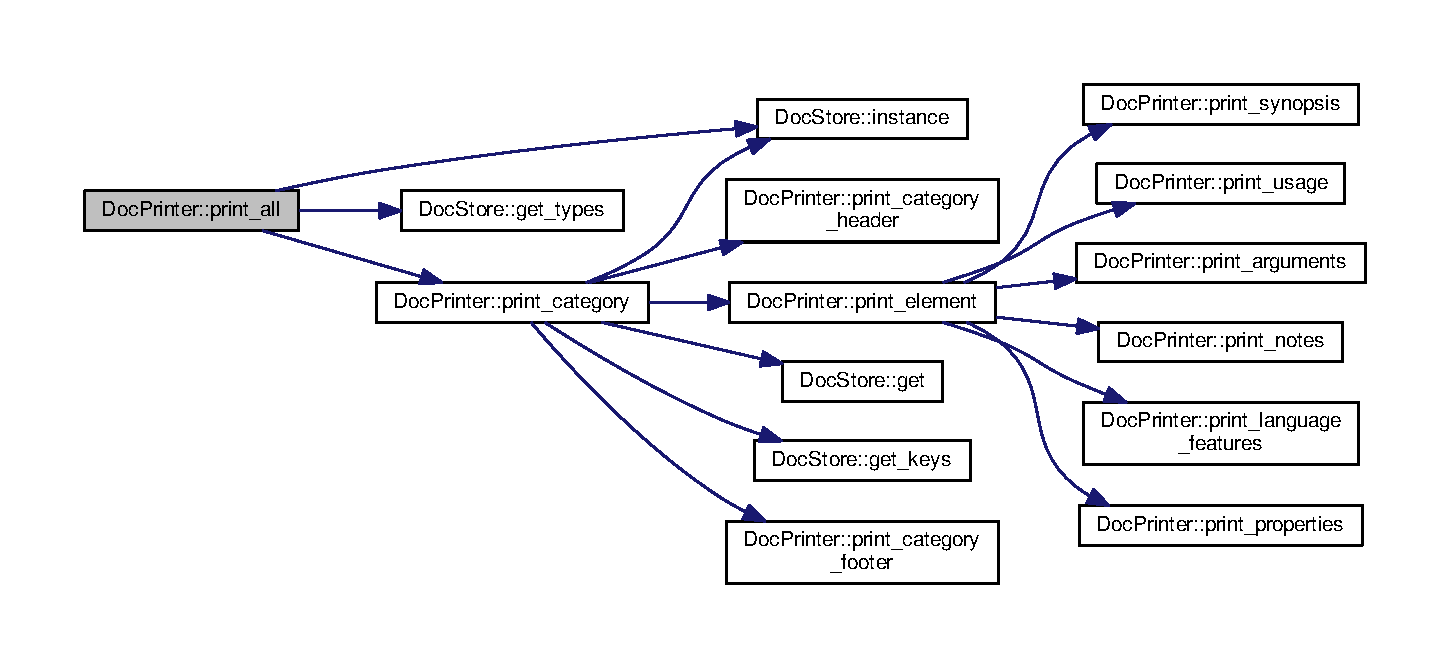
\includegraphics[width=350pt]{classDocPrinter_a7da00e32e5758f07b5a1b6cd5d4e9824_cgraph}
\end{center}
\end{figure}


\hypertarget{classDocPrinter_a9e8339a87ec6aa5bc11017eec937372c}{\index{Doc\-Printer@{Doc\-Printer}!print\-\_\-arguments@{print\-\_\-arguments}}
\index{print\-\_\-arguments@{print\-\_\-arguments}!DocPrinter@{Doc\-Printer}}
\subsubsection[{print\-\_\-arguments}]{\setlength{\rightskip}{0pt plus 5cm}virtual void Doc\-Printer\-::print\-\_\-arguments (
\begin{DoxyParamCaption}
\item[{const {\bf Doc\-Struct} \&}]{info}
\end{DoxyParamCaption}
)\hspace{0.3cm}{\ttfamily [protected]}, {\ttfamily [pure virtual]}}}\label{classDocPrinter_a9e8339a87ec6aa5bc11017eec937372c}


Implemented in \hyperlink{classPlainPrinter_a6eb1b927ed5dd5f3604041872110e51a}{Plain\-Printer}, and \hyperlink{classTxt2TagsPrinter_a211dc59422b4a7bed65e27ac9e2aff11}{Txt2\-Tags\-Printer}.

\hypertarget{classDocPrinter_a70234bd56a73aa917edf170be8415ce6}{\index{Doc\-Printer@{Doc\-Printer}!print\-\_\-category@{print\-\_\-category}}
\index{print\-\_\-category@{print\-\_\-category}!DocPrinter@{Doc\-Printer}}
\subsubsection[{print\-\_\-category}]{\setlength{\rightskip}{0pt plus 5cm}void Doc\-Printer\-::print\-\_\-category (
\begin{DoxyParamCaption}
\item[{std\-::string}]{category\-\_\-name}
\end{DoxyParamCaption}
)\hspace{0.3cm}{\ttfamily [virtual]}}}\label{classDocPrinter_a70234bd56a73aa917edf170be8415ce6}


Here is the call graph for this function\-:
\nopagebreak
\begin{figure}[H]
\begin{center}
\leavevmode
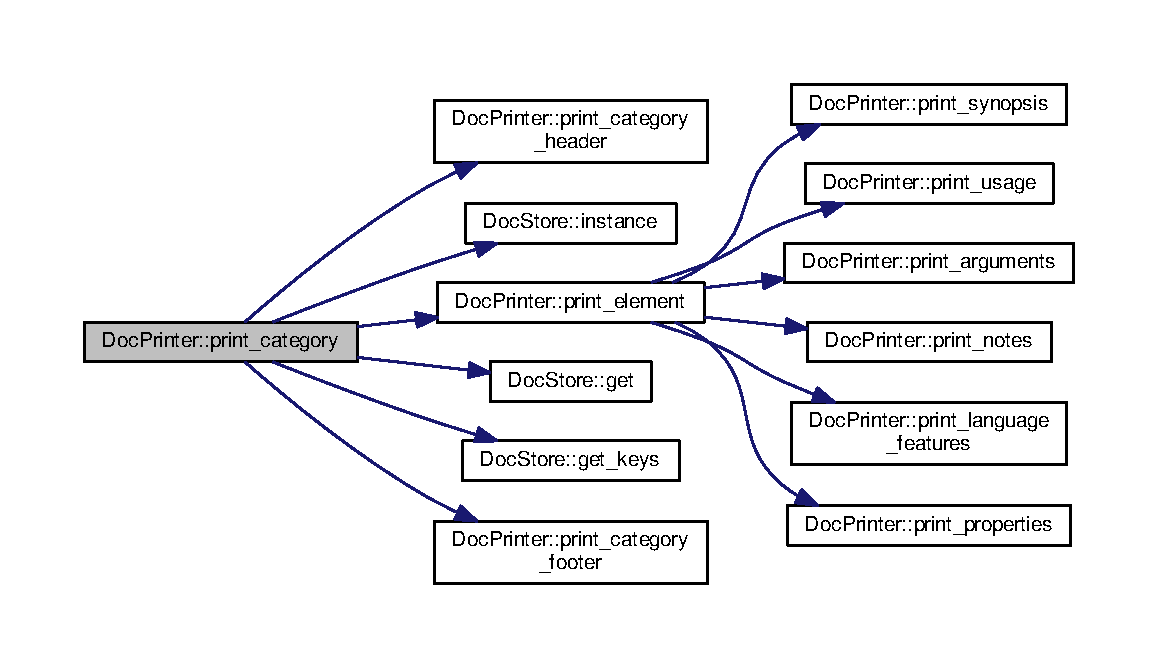
\includegraphics[width=350pt]{classDocPrinter_a70234bd56a73aa917edf170be8415ce6_cgraph}
\end{center}
\end{figure}


\hypertarget{classDocPrinter_aa96cf13e25fdd6cb854b0efb8e89046a}{\index{Doc\-Printer@{Doc\-Printer}!print\-\_\-category\-\_\-footer@{print\-\_\-category\-\_\-footer}}
\index{print\-\_\-category\-\_\-footer@{print\-\_\-category\-\_\-footer}!DocPrinter@{Doc\-Printer}}
\subsubsection[{print\-\_\-category\-\_\-footer}]{\setlength{\rightskip}{0pt plus 5cm}virtual void Doc\-Printer\-::print\-\_\-category\-\_\-footer (
\begin{DoxyParamCaption}
{}
\end{DoxyParamCaption}
)\hspace{0.3cm}{\ttfamily [protected]}, {\ttfamily [pure virtual]}}}\label{classDocPrinter_aa96cf13e25fdd6cb854b0efb8e89046a}


Implemented in \hyperlink{classPlainPrinter_a324d849386ce24478f5711b2fc3b26c2}{Plain\-Printer}, and \hyperlink{classTxt2TagsPrinter_ae937c09e8f3eeb2fb30c118facf60a7e}{Txt2\-Tags\-Printer}.

\hypertarget{classDocPrinter_a7a8d538ac102b331f891b4cd86c814ab}{\index{Doc\-Printer@{Doc\-Printer}!print\-\_\-category\-\_\-header@{print\-\_\-category\-\_\-header}}
\index{print\-\_\-category\-\_\-header@{print\-\_\-category\-\_\-header}!DocPrinter@{Doc\-Printer}}
\subsubsection[{print\-\_\-category\-\_\-header}]{\setlength{\rightskip}{0pt plus 5cm}virtual void Doc\-Printer\-::print\-\_\-category\-\_\-header (
\begin{DoxyParamCaption}
\item[{std\-::string}]{category\-\_\-name}
\end{DoxyParamCaption}
)\hspace{0.3cm}{\ttfamily [protected]}, {\ttfamily [pure virtual]}}}\label{classDocPrinter_a7a8d538ac102b331f891b4cd86c814ab}


Implemented in \hyperlink{classPlainPrinter_a860ced811a6309d1889ab926ebdd4f67}{Plain\-Printer}, and \hyperlink{classTxt2TagsPrinter_a272f9f74d06e9926b9de61c96e02ecd7}{Txt2\-Tags\-Printer}.

\hypertarget{classDocPrinter_a0253343f6a7ffef9de4c915d2091d5db}{\index{Doc\-Printer@{Doc\-Printer}!print\-\_\-element@{print\-\_\-element}}
\index{print\-\_\-element@{print\-\_\-element}!DocPrinter@{Doc\-Printer}}
\subsubsection[{print\-\_\-element}]{\setlength{\rightskip}{0pt plus 5cm}void Doc\-Printer\-::print\-\_\-element (
\begin{DoxyParamCaption}
\item[{std\-::string}]{call\-\_\-name, }
\item[{const {\bf Doc\-Struct} \&}]{info}
\end{DoxyParamCaption}
)\hspace{0.3cm}{\ttfamily [virtual]}}}\label{classDocPrinter_a0253343f6a7ffef9de4c915d2091d5db}


Here is the call graph for this function\-:
\nopagebreak
\begin{figure}[H]
\begin{center}
\leavevmode
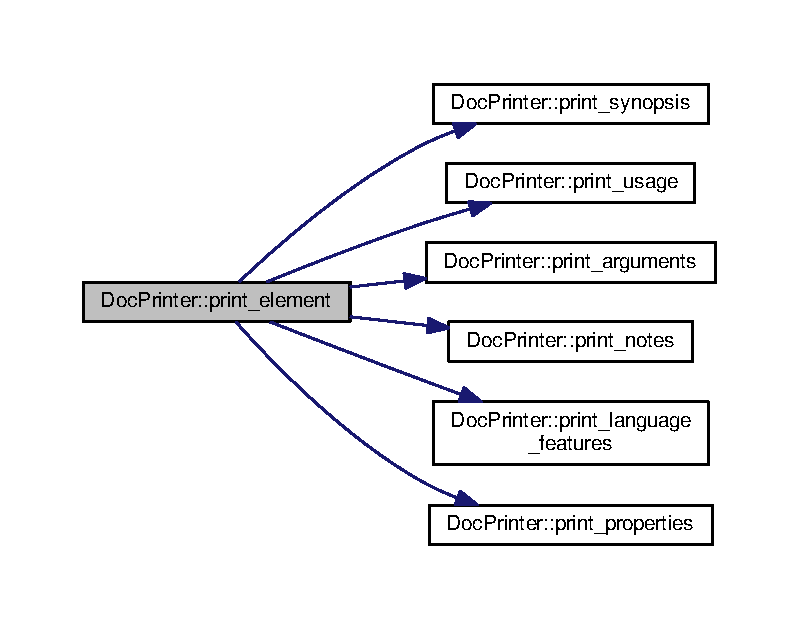
\includegraphics[width=350pt]{classDocPrinter_a0253343f6a7ffef9de4c915d2091d5db_cgraph}
\end{center}
\end{figure}


\hypertarget{classDocPrinter_aba345d8b3a03bca1aa7c2363260dfdf8}{\index{Doc\-Printer@{Doc\-Printer}!print\-\_\-language\-\_\-features@{print\-\_\-language\-\_\-features}}
\index{print\-\_\-language\-\_\-features@{print\-\_\-language\-\_\-features}!DocPrinter@{Doc\-Printer}}
\subsubsection[{print\-\_\-language\-\_\-features}]{\setlength{\rightskip}{0pt plus 5cm}virtual void Doc\-Printer\-::print\-\_\-language\-\_\-features (
\begin{DoxyParamCaption}
\item[{const {\bf Doc\-Struct} \&}]{info}
\end{DoxyParamCaption}
)\hspace{0.3cm}{\ttfamily [protected]}, {\ttfamily [pure virtual]}}}\label{classDocPrinter_aba345d8b3a03bca1aa7c2363260dfdf8}


Implemented in \hyperlink{classPlainPrinter_aa20ff6c29f9cffad1522892485316775}{Plain\-Printer}, and \hyperlink{classTxt2TagsPrinter_a330214e600158887ef50f012523b8f32}{Txt2\-Tags\-Printer}.

\hypertarget{classDocPrinter_ae53baee3061725f2d2e02c75c6e8a5a3}{\index{Doc\-Printer@{Doc\-Printer}!print\-\_\-notes@{print\-\_\-notes}}
\index{print\-\_\-notes@{print\-\_\-notes}!DocPrinter@{Doc\-Printer}}
\subsubsection[{print\-\_\-notes}]{\setlength{\rightskip}{0pt plus 5cm}virtual void Doc\-Printer\-::print\-\_\-notes (
\begin{DoxyParamCaption}
\item[{const {\bf Doc\-Struct} \&}]{info}
\end{DoxyParamCaption}
)\hspace{0.3cm}{\ttfamily [protected]}, {\ttfamily [pure virtual]}}}\label{classDocPrinter_ae53baee3061725f2d2e02c75c6e8a5a3}


Implemented in \hyperlink{classPlainPrinter_a105fabd1f37aa1d99e4272e3ebb4d3b8}{Plain\-Printer}, and \hyperlink{classTxt2TagsPrinter_a2c966dac44b8926523a956c37b073870}{Txt2\-Tags\-Printer}.

\hypertarget{classDocPrinter_a16854272b22ca9129f9afb9c42157736}{\index{Doc\-Printer@{Doc\-Printer}!print\-\_\-properties@{print\-\_\-properties}}
\index{print\-\_\-properties@{print\-\_\-properties}!DocPrinter@{Doc\-Printer}}
\subsubsection[{print\-\_\-properties}]{\setlength{\rightskip}{0pt plus 5cm}virtual void Doc\-Printer\-::print\-\_\-properties (
\begin{DoxyParamCaption}
\item[{const {\bf Doc\-Struct} \&}]{info}
\end{DoxyParamCaption}
)\hspace{0.3cm}{\ttfamily [protected]}, {\ttfamily [pure virtual]}}}\label{classDocPrinter_a16854272b22ca9129f9afb9c42157736}


Implemented in \hyperlink{classPlainPrinter_a0768f7e6781dfaebf0e54535f1031467}{Plain\-Printer}, and \hyperlink{classTxt2TagsPrinter_abcf56c43f241406e207861f98c58fb3c}{Txt2\-Tags\-Printer}.

\hypertarget{classDocPrinter_abb2a5b5121292d292ff682f94e187534}{\index{Doc\-Printer@{Doc\-Printer}!print\-\_\-synopsis@{print\-\_\-synopsis}}
\index{print\-\_\-synopsis@{print\-\_\-synopsis}!DocPrinter@{Doc\-Printer}}
\subsubsection[{print\-\_\-synopsis}]{\setlength{\rightskip}{0pt plus 5cm}virtual void Doc\-Printer\-::print\-\_\-synopsis (
\begin{DoxyParamCaption}
\item[{const {\bf Doc\-Struct} \&}]{info}
\end{DoxyParamCaption}
)\hspace{0.3cm}{\ttfamily [protected]}, {\ttfamily [pure virtual]}}}\label{classDocPrinter_abb2a5b5121292d292ff682f94e187534}


Implemented in \hyperlink{classPlainPrinter_ac998df8a56c056800eda2c1d9ca3f628}{Plain\-Printer}, and \hyperlink{classTxt2TagsPrinter_a6bcc28d9a842cdb08f2f20b857480d7f}{Txt2\-Tags\-Printer}.

\hypertarget{classDocPrinter_aa967b483b8def39d7ba5f039bd3c4acd}{\index{Doc\-Printer@{Doc\-Printer}!print\-\_\-usage@{print\-\_\-usage}}
\index{print\-\_\-usage@{print\-\_\-usage}!DocPrinter@{Doc\-Printer}}
\subsubsection[{print\-\_\-usage}]{\setlength{\rightskip}{0pt plus 5cm}virtual void Doc\-Printer\-::print\-\_\-usage (
\begin{DoxyParamCaption}
\item[{std\-::string}]{call\-\_\-name, }
\item[{const {\bf Doc\-Struct} \&}]{info}
\end{DoxyParamCaption}
)\hspace{0.3cm}{\ttfamily [protected]}, {\ttfamily [pure virtual]}}}\label{classDocPrinter_aa967b483b8def39d7ba5f039bd3c4acd}


Implemented in \hyperlink{classPlainPrinter_ab5478f9542ccf99138668975ab3192d8}{Plain\-Printer}, and \hyperlink{classTxt2TagsPrinter_a1052b10fce569cf5a7dd8d2071e58987}{Txt2\-Tags\-Printer}.



\subsection{Member Data Documentation}
\hypertarget{classDocPrinter_a30860614cca992c360838670c209eb00}{\index{Doc\-Printer@{Doc\-Printer}!os@{os}}
\index{os@{os}!DocPrinter@{Doc\-Printer}}
\subsubsection[{os}]{\setlength{\rightskip}{0pt plus 5cm}std\-::ostream\& Doc\-Printer\-::os\hspace{0.3cm}{\ttfamily [protected]}}}\label{classDocPrinter_a30860614cca992c360838670c209eb00}


The documentation for this class was generated from the following files\-:\begin{DoxyCompactItemize}
\item 
\hyperlink{option__parser__util_8h}{option\-\_\-parser\-\_\-util.\-h}\item 
\hyperlink{option__parser__util_8cc}{option\-\_\-parser\-\_\-util.\-cc}\end{DoxyCompactItemize}

\hypertarget{classDocStore}{\section{Doc\-Store Class Reference}
\label{classDocStore}\index{Doc\-Store@{Doc\-Store}}
}


{\ttfamily \#include $<$option\-\_\-parser\-\_\-util.\-h$>$}

\subsection*{Public Member Functions}
\begin{DoxyCompactItemize}
\item 
void \hyperlink{classDocStore_a8b4c9409f58c965696b9b40f3c3566a6}{register\-\_\-object} (std\-::string k, std\-::string type)
\item 
void \hyperlink{classDocStore_ae14a668d96193c54cc7356a7e6dfe5ad}{add\-\_\-arg} (std\-::string k, std\-::string arg\-\_\-name, std\-::string help, std\-::string type, std\-::string default\-\_\-value, bool mandatory, \hyperlink{option__parser__util_8h_a916a9983a28a9efe2c606860052d5fe0}{Value\-Explanations} value\-\_\-explanations=\hyperlink{option__parser__util_8h_a916a9983a28a9efe2c606860052d5fe0}{Value\-Explanations}())
\item 
void \hyperlink{classDocStore_acb52135c577a1f483d0a716b1b8eee19}{add\-\_\-value\-\_\-explanations} (std\-::string k, std\-::string arg\-\_\-name, \hyperlink{option__parser__util_8h_a916a9983a28a9efe2c606860052d5fe0}{Value\-Explanations} value\-\_\-explanations)
\item 
void \hyperlink{classDocStore_ab1bb67c5d977b5f08784cb7342b5d082}{set\-\_\-synopsis} (std\-::string k, std\-::string name, std\-::string description)
\item 
void \hyperlink{classDocStore_a345d2e581ecec6a9449143bafec7b5a7}{add\-\_\-property} (std\-::string k, std\-::string name, std\-::string description)
\item 
void \hyperlink{classDocStore_a5f281c8bb7798d9fc7831cdf6602657f}{add\-\_\-feature} (std\-::string k, std\-::string feature, std\-::string description)
\item 
void \hyperlink{classDocStore_a8989ea881e708cfbb0876bd440d5c239}{add\-\_\-note} (std\-::string k, std\-::string name, std\-::string description, bool long\-\_\-text)
\item 
void \hyperlink{classDocStore_a1311dd8bd79cc4f549e4dc24f804af0b}{hide} (std\-::string k)
\item 
bool \hyperlink{classDocStore_a1ff4c822e32354a092b93ecaa394779a}{contains} (std\-::string k)
\item 
\hyperlink{structDocStruct}{Doc\-Struct} \hyperlink{classDocStore_aa41ed6e54cf6c61332cb0d037731593d}{get} (std\-::string k)
\item 
std\-::vector$<$ std\-::string $>$ \hyperlink{classDocStore_ace9674ccb03fa34d70ab2ced166d2e89}{get\-\_\-keys} ()
\item 
std\-::vector$<$ std\-::string $>$ \hyperlink{classDocStore_affba2ace14efcd69680d4b01bc57a28e}{get\-\_\-types} ()
\end{DoxyCompactItemize}
\subsection*{Static Public Member Functions}
\begin{DoxyCompactItemize}
\item 
static \hyperlink{classDocStore}{Doc\-Store} $\ast$ \hyperlink{classDocStore_a55af131cd6b424f7c7e1ccadf77dca5f}{instance} ()
\end{DoxyCompactItemize}


\subsection{Member Function Documentation}
\hypertarget{classDocStore_ae14a668d96193c54cc7356a7e6dfe5ad}{\index{Doc\-Store@{Doc\-Store}!add\-\_\-arg@{add\-\_\-arg}}
\index{add\-\_\-arg@{add\-\_\-arg}!DocStore@{Doc\-Store}}
\subsubsection[{add\-\_\-arg}]{\setlength{\rightskip}{0pt plus 5cm}void Doc\-Store\-::add\-\_\-arg (
\begin{DoxyParamCaption}
\item[{std\-::string}]{k, }
\item[{std\-::string}]{arg\-\_\-name, }
\item[{std\-::string}]{help, }
\item[{std\-::string}]{type, }
\item[{std\-::string}]{default\-\_\-value, }
\item[{bool}]{mandatory, }
\item[{{\bf Value\-Explanations}}]{value\-\_\-explanations = {\ttfamily {\bf Value\-Explanations}()}}
\end{DoxyParamCaption}
)}}\label{classDocStore_ae14a668d96193c54cc7356a7e6dfe5ad}
\hypertarget{classDocStore_a5f281c8bb7798d9fc7831cdf6602657f}{\index{Doc\-Store@{Doc\-Store}!add\-\_\-feature@{add\-\_\-feature}}
\index{add\-\_\-feature@{add\-\_\-feature}!DocStore@{Doc\-Store}}
\subsubsection[{add\-\_\-feature}]{\setlength{\rightskip}{0pt plus 5cm}void Doc\-Store\-::add\-\_\-feature (
\begin{DoxyParamCaption}
\item[{std\-::string}]{k, }
\item[{std\-::string}]{feature, }
\item[{std\-::string}]{description}
\end{DoxyParamCaption}
)}}\label{classDocStore_a5f281c8bb7798d9fc7831cdf6602657f}
\hypertarget{classDocStore_a8989ea881e708cfbb0876bd440d5c239}{\index{Doc\-Store@{Doc\-Store}!add\-\_\-note@{add\-\_\-note}}
\index{add\-\_\-note@{add\-\_\-note}!DocStore@{Doc\-Store}}
\subsubsection[{add\-\_\-note}]{\setlength{\rightskip}{0pt plus 5cm}void Doc\-Store\-::add\-\_\-note (
\begin{DoxyParamCaption}
\item[{std\-::string}]{k, }
\item[{std\-::string}]{name, }
\item[{std\-::string}]{description, }
\item[{bool}]{long\-\_\-text}
\end{DoxyParamCaption}
)}}\label{classDocStore_a8989ea881e708cfbb0876bd440d5c239}
\hypertarget{classDocStore_a345d2e581ecec6a9449143bafec7b5a7}{\index{Doc\-Store@{Doc\-Store}!add\-\_\-property@{add\-\_\-property}}
\index{add\-\_\-property@{add\-\_\-property}!DocStore@{Doc\-Store}}
\subsubsection[{add\-\_\-property}]{\setlength{\rightskip}{0pt plus 5cm}void Doc\-Store\-::add\-\_\-property (
\begin{DoxyParamCaption}
\item[{std\-::string}]{k, }
\item[{std\-::string}]{name, }
\item[{std\-::string}]{description}
\end{DoxyParamCaption}
)}}\label{classDocStore_a345d2e581ecec6a9449143bafec7b5a7}
\hypertarget{classDocStore_acb52135c577a1f483d0a716b1b8eee19}{\index{Doc\-Store@{Doc\-Store}!add\-\_\-value\-\_\-explanations@{add\-\_\-value\-\_\-explanations}}
\index{add\-\_\-value\-\_\-explanations@{add\-\_\-value\-\_\-explanations}!DocStore@{Doc\-Store}}
\subsubsection[{add\-\_\-value\-\_\-explanations}]{\setlength{\rightskip}{0pt plus 5cm}void Doc\-Store\-::add\-\_\-value\-\_\-explanations (
\begin{DoxyParamCaption}
\item[{std\-::string}]{k, }
\item[{std\-::string}]{arg\-\_\-name, }
\item[{{\bf Value\-Explanations}}]{value\-\_\-explanations}
\end{DoxyParamCaption}
)}}\label{classDocStore_acb52135c577a1f483d0a716b1b8eee19}
\hypertarget{classDocStore_a1ff4c822e32354a092b93ecaa394779a}{\index{Doc\-Store@{Doc\-Store}!contains@{contains}}
\index{contains@{contains}!DocStore@{Doc\-Store}}
\subsubsection[{contains}]{\setlength{\rightskip}{0pt plus 5cm}bool Doc\-Store\-::contains (
\begin{DoxyParamCaption}
\item[{std\-::string}]{k}
\end{DoxyParamCaption}
)}}\label{classDocStore_a1ff4c822e32354a092b93ecaa394779a}
\hypertarget{classDocStore_aa41ed6e54cf6c61332cb0d037731593d}{\index{Doc\-Store@{Doc\-Store}!get@{get}}
\index{get@{get}!DocStore@{Doc\-Store}}
\subsubsection[{get}]{\setlength{\rightskip}{0pt plus 5cm}{\bf Doc\-Struct} Doc\-Store\-::get (
\begin{DoxyParamCaption}
\item[{std\-::string}]{k}
\end{DoxyParamCaption}
)}}\label{classDocStore_aa41ed6e54cf6c61332cb0d037731593d}
\hypertarget{classDocStore_ace9674ccb03fa34d70ab2ced166d2e89}{\index{Doc\-Store@{Doc\-Store}!get\-\_\-keys@{get\-\_\-keys}}
\index{get\-\_\-keys@{get\-\_\-keys}!DocStore@{Doc\-Store}}
\subsubsection[{get\-\_\-keys}]{\setlength{\rightskip}{0pt plus 5cm}vector$<$ string $>$ Doc\-Store\-::get\-\_\-keys (
\begin{DoxyParamCaption}
{}
\end{DoxyParamCaption}
)}}\label{classDocStore_ace9674ccb03fa34d70ab2ced166d2e89}
\hypertarget{classDocStore_affba2ace14efcd69680d4b01bc57a28e}{\index{Doc\-Store@{Doc\-Store}!get\-\_\-types@{get\-\_\-types}}
\index{get\-\_\-types@{get\-\_\-types}!DocStore@{Doc\-Store}}
\subsubsection[{get\-\_\-types}]{\setlength{\rightskip}{0pt plus 5cm}vector$<$ string $>$ Doc\-Store\-::get\-\_\-types (
\begin{DoxyParamCaption}
{}
\end{DoxyParamCaption}
)}}\label{classDocStore_affba2ace14efcd69680d4b01bc57a28e}
\hypertarget{classDocStore_a1311dd8bd79cc4f549e4dc24f804af0b}{\index{Doc\-Store@{Doc\-Store}!hide@{hide}}
\index{hide@{hide}!DocStore@{Doc\-Store}}
\subsubsection[{hide}]{\setlength{\rightskip}{0pt plus 5cm}void Doc\-Store\-::hide (
\begin{DoxyParamCaption}
\item[{std\-::string}]{k}
\end{DoxyParamCaption}
)}}\label{classDocStore_a1311dd8bd79cc4f549e4dc24f804af0b}
\hypertarget{classDocStore_a55af131cd6b424f7c7e1ccadf77dca5f}{\index{Doc\-Store@{Doc\-Store}!instance@{instance}}
\index{instance@{instance}!DocStore@{Doc\-Store}}
\subsubsection[{instance}]{\setlength{\rightskip}{0pt plus 5cm}static {\bf Doc\-Store}$\ast$ Doc\-Store\-::instance (
\begin{DoxyParamCaption}
{}
\end{DoxyParamCaption}
)\hspace{0.3cm}{\ttfamily [inline]}, {\ttfamily [static]}}}\label{classDocStore_a55af131cd6b424f7c7e1ccadf77dca5f}
\hypertarget{classDocStore_a8b4c9409f58c965696b9b40f3c3566a6}{\index{Doc\-Store@{Doc\-Store}!register\-\_\-object@{register\-\_\-object}}
\index{register\-\_\-object@{register\-\_\-object}!DocStore@{Doc\-Store}}
\subsubsection[{register\-\_\-object}]{\setlength{\rightskip}{0pt plus 5cm}void Doc\-Store\-::register\-\_\-object (
\begin{DoxyParamCaption}
\item[{std\-::string}]{k, }
\item[{std\-::string}]{type}
\end{DoxyParamCaption}
)}}\label{classDocStore_a8b4c9409f58c965696b9b40f3c3566a6}
\hypertarget{classDocStore_ab1bb67c5d977b5f08784cb7342b5d082}{\index{Doc\-Store@{Doc\-Store}!set\-\_\-synopsis@{set\-\_\-synopsis}}
\index{set\-\_\-synopsis@{set\-\_\-synopsis}!DocStore@{Doc\-Store}}
\subsubsection[{set\-\_\-synopsis}]{\setlength{\rightskip}{0pt plus 5cm}void Doc\-Store\-::set\-\_\-synopsis (
\begin{DoxyParamCaption}
\item[{std\-::string}]{k, }
\item[{std\-::string}]{name, }
\item[{std\-::string}]{description}
\end{DoxyParamCaption}
)}}\label{classDocStore_ab1bb67c5d977b5f08784cb7342b5d082}


The documentation for this class was generated from the following files\-:\begin{DoxyCompactItemize}
\item 
\hyperlink{option__parser__util_8h}{option\-\_\-parser\-\_\-util.\-h}\item 
\hyperlink{option__parser__util_8cc}{option\-\_\-parser\-\_\-util.\-cc}\end{DoxyCompactItemize}

\hypertarget{structDocStruct}{\section{Doc\-Struct Struct Reference}
\label{structDocStruct}\index{Doc\-Struct@{Doc\-Struct}}
}


{\ttfamily \#include $<$option\-\_\-parser\-\_\-util.\-h$>$}

\subsection*{Public Attributes}
\begin{DoxyCompactItemize}
\item 
std\-::string \hyperlink{structDocStruct_a91a29979c17e21f606349d0450a75e8e}{type}
\item 
std\-::string \hyperlink{structDocStruct_ab8f7dbf05b414a94c4378b783270cf1e}{full\-\_\-name}
\item 
std\-::string \hyperlink{structDocStruct_af808bfe418f51eacf0c1101513d3677f}{synopsis}
\item 
std\-::vector$<$ \hyperlink{structArgumentInfo}{Argument\-Info} $>$ \hyperlink{structDocStruct_aaf770bc3b8bbe01f8a0a0e859fdf0c92}{arg\-\_\-help}
\item 
std\-::vector$<$ \hyperlink{structPropertyInfo}{Property\-Info} $>$ \hyperlink{structDocStruct_a9eb6464706fd52b152dd73560919b41b}{property\-\_\-help}
\item 
std\-::vector$<$ \hyperlink{structLanguageSupportInfo}{Language\-Support\-Info} $>$ \hyperlink{structDocStruct_a5ab754df0511c5d44c26063e59472b6b}{support\-\_\-help}
\item 
std\-::vector$<$ \hyperlink{structNoteInfo}{Note\-Info} $>$ \hyperlink{structDocStruct_a511a4d9eac3411c758b2ea6817421692}{notes}
\item 
bool \hyperlink{structDocStruct_af440a5475a918a0ab6cac5ea7dc38421}{hidden}
\end{DoxyCompactItemize}


\subsection{Member Data Documentation}
\hypertarget{structDocStruct_aaf770bc3b8bbe01f8a0a0e859fdf0c92}{\index{Doc\-Struct@{Doc\-Struct}!arg\-\_\-help@{arg\-\_\-help}}
\index{arg\-\_\-help@{arg\-\_\-help}!DocStruct@{Doc\-Struct}}
\subsubsection[{arg\-\_\-help}]{\setlength{\rightskip}{0pt plus 5cm}std\-::vector$<${\bf Argument\-Info}$>$ Doc\-Struct\-::arg\-\_\-help}}\label{structDocStruct_aaf770bc3b8bbe01f8a0a0e859fdf0c92}
\hypertarget{structDocStruct_ab8f7dbf05b414a94c4378b783270cf1e}{\index{Doc\-Struct@{Doc\-Struct}!full\-\_\-name@{full\-\_\-name}}
\index{full\-\_\-name@{full\-\_\-name}!DocStruct@{Doc\-Struct}}
\subsubsection[{full\-\_\-name}]{\setlength{\rightskip}{0pt plus 5cm}std\-::string Doc\-Struct\-::full\-\_\-name}}\label{structDocStruct_ab8f7dbf05b414a94c4378b783270cf1e}
\hypertarget{structDocStruct_af440a5475a918a0ab6cac5ea7dc38421}{\index{Doc\-Struct@{Doc\-Struct}!hidden@{hidden}}
\index{hidden@{hidden}!DocStruct@{Doc\-Struct}}
\subsubsection[{hidden}]{\setlength{\rightskip}{0pt plus 5cm}bool Doc\-Struct\-::hidden}}\label{structDocStruct_af440a5475a918a0ab6cac5ea7dc38421}
\hypertarget{structDocStruct_a511a4d9eac3411c758b2ea6817421692}{\index{Doc\-Struct@{Doc\-Struct}!notes@{notes}}
\index{notes@{notes}!DocStruct@{Doc\-Struct}}
\subsubsection[{notes}]{\setlength{\rightskip}{0pt plus 5cm}std\-::vector$<${\bf Note\-Info}$>$ Doc\-Struct\-::notes}}\label{structDocStruct_a511a4d9eac3411c758b2ea6817421692}
\hypertarget{structDocStruct_a9eb6464706fd52b152dd73560919b41b}{\index{Doc\-Struct@{Doc\-Struct}!property\-\_\-help@{property\-\_\-help}}
\index{property\-\_\-help@{property\-\_\-help}!DocStruct@{Doc\-Struct}}
\subsubsection[{property\-\_\-help}]{\setlength{\rightskip}{0pt plus 5cm}std\-::vector$<${\bf Property\-Info}$>$ Doc\-Struct\-::property\-\_\-help}}\label{structDocStruct_a9eb6464706fd52b152dd73560919b41b}
\hypertarget{structDocStruct_a5ab754df0511c5d44c26063e59472b6b}{\index{Doc\-Struct@{Doc\-Struct}!support\-\_\-help@{support\-\_\-help}}
\index{support\-\_\-help@{support\-\_\-help}!DocStruct@{Doc\-Struct}}
\subsubsection[{support\-\_\-help}]{\setlength{\rightskip}{0pt plus 5cm}std\-::vector$<${\bf Language\-Support\-Info}$>$ Doc\-Struct\-::support\-\_\-help}}\label{structDocStruct_a5ab754df0511c5d44c26063e59472b6b}
\hypertarget{structDocStruct_af808bfe418f51eacf0c1101513d3677f}{\index{Doc\-Struct@{Doc\-Struct}!synopsis@{synopsis}}
\index{synopsis@{synopsis}!DocStruct@{Doc\-Struct}}
\subsubsection[{synopsis}]{\setlength{\rightskip}{0pt plus 5cm}std\-::string Doc\-Struct\-::synopsis}}\label{structDocStruct_af808bfe418f51eacf0c1101513d3677f}
\hypertarget{structDocStruct_a91a29979c17e21f606349d0450a75e8e}{\index{Doc\-Struct@{Doc\-Struct}!type@{type}}
\index{type@{type}!DocStruct@{Doc\-Struct}}
\subsubsection[{type}]{\setlength{\rightskip}{0pt plus 5cm}std\-::string Doc\-Struct\-::type}}\label{structDocStruct_a91a29979c17e21f606349d0450a75e8e}


The documentation for this struct was generated from the following file\-:\begin{DoxyCompactItemize}
\item 
\hyperlink{option__parser__util_8h}{option\-\_\-parser\-\_\-util.\-h}\end{DoxyCompactItemize}

\hypertarget{classDomainTransitionGraph}{\section{Domain\-Transition\-Graph Class Reference}
\label{classDomainTransitionGraph}\index{Domain\-Transition\-Graph@{Domain\-Transition\-Graph}}
}


{\ttfamily \#include $<$domain\-\_\-transition\-\_\-graph.\-h$>$}

\subsection*{Public Member Functions}
\begin{DoxyCompactItemize}
\item 
\hyperlink{classDomainTransitionGraph_a936f3aae8f284484bf3ef1a2f4e7e956}{Domain\-Transition\-Graph} (int var\-\_\-index, int node\-\_\-count)
\item 
void \hyperlink{classDomainTransitionGraph_a80221d83ff7109b5f5b64a8851a4a075}{read\-\_\-data} (istream \&in)
\item 
void \hyperlink{classDomainTransitionGraph_a412189c6fdd8904ee158b10d1c26b35e}{dump} () const 
\item 
void \hyperlink{classDomainTransitionGraph_a3b669495247f768863f47b1c28a61951}{get\-\_\-successors} (int value, vector$<$ int $>$ \&result) const 
\end{DoxyCompactItemize}
\subsection*{Static Public Member Functions}
\begin{DoxyCompactItemize}
\item 
static void \hyperlink{classDomainTransitionGraph_aba53fff6f1e933d0fded474ef2d6182f}{read\-\_\-all} (istream \&in)
\end{DoxyCompactItemize}
\subsection*{Friends}
\begin{DoxyCompactItemize}
\item 
class \hyperlink{classDomainTransitionGraph_af48a2cc498085d9855e0a1d95b8ee7b4}{C\-G\-Heuristic}
\item 
class \hyperlink{classDomainTransitionGraph_acb8e7e5543a9e3929bf2d038d3a30a20}{cea\-\_\-heuristic\-::\-Context\-Enhanced\-Additive\-Heuristic}
\item 
struct \hyperlink{classDomainTransitionGraph_a111633b0408f9645dc6e3f8233f2511a}{Value\-Node}
\item 
struct \hyperlink{classDomainTransitionGraph_a14fe5a6c4d0b0fe3d17004e5a8daab2f}{Value\-Transition}
\item 
struct \hyperlink{classDomainTransitionGraph_aa088a060547b679aea38e0bc3accf661}{Local\-Assignment}
\end{DoxyCompactItemize}


\subsection{Constructor \& Destructor Documentation}
\hypertarget{classDomainTransitionGraph_a936f3aae8f284484bf3ef1a2f4e7e956}{\index{Domain\-Transition\-Graph@{Domain\-Transition\-Graph}!Domain\-Transition\-Graph@{Domain\-Transition\-Graph}}
\index{Domain\-Transition\-Graph@{Domain\-Transition\-Graph}!DomainTransitionGraph@{Domain\-Transition\-Graph}}
\subsubsection[{Domain\-Transition\-Graph}]{\setlength{\rightskip}{0pt plus 5cm}Domain\-Transition\-Graph\-::\-Domain\-Transition\-Graph (
\begin{DoxyParamCaption}
\item[{int}]{var\-\_\-index, }
\item[{int}]{node\-\_\-count}
\end{DoxyParamCaption}
)}}\label{classDomainTransitionGraph_a936f3aae8f284484bf3ef1a2f4e7e956}


\subsection{Member Function Documentation}
\hypertarget{classDomainTransitionGraph_a412189c6fdd8904ee158b10d1c26b35e}{\index{Domain\-Transition\-Graph@{Domain\-Transition\-Graph}!dump@{dump}}
\index{dump@{dump}!DomainTransitionGraph@{Domain\-Transition\-Graph}}
\subsubsection[{dump}]{\setlength{\rightskip}{0pt plus 5cm}void Domain\-Transition\-Graph\-::dump (
\begin{DoxyParamCaption}
{}
\end{DoxyParamCaption}
) const}}\label{classDomainTransitionGraph_a412189c6fdd8904ee158b10d1c26b35e}
\hypertarget{classDomainTransitionGraph_a3b669495247f768863f47b1c28a61951}{\index{Domain\-Transition\-Graph@{Domain\-Transition\-Graph}!get\-\_\-successors@{get\-\_\-successors}}
\index{get\-\_\-successors@{get\-\_\-successors}!DomainTransitionGraph@{Domain\-Transition\-Graph}}
\subsubsection[{get\-\_\-successors}]{\setlength{\rightskip}{0pt plus 5cm}void Domain\-Transition\-Graph\-::get\-\_\-successors (
\begin{DoxyParamCaption}
\item[{int}]{value, }
\item[{vector$<$ int $>$ \&}]{result}
\end{DoxyParamCaption}
) const}}\label{classDomainTransitionGraph_a3b669495247f768863f47b1c28a61951}


Here is the call graph for this function\-:
\nopagebreak
\begin{figure}[H]
\begin{center}
\leavevmode
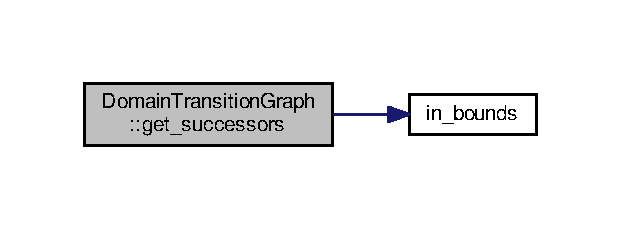
\includegraphics[width=298pt]{classDomainTransitionGraph_a3b669495247f768863f47b1c28a61951_cgraph}
\end{center}
\end{figure}


\hypertarget{classDomainTransitionGraph_aba53fff6f1e933d0fded474ef2d6182f}{\index{Domain\-Transition\-Graph@{Domain\-Transition\-Graph}!read\-\_\-all@{read\-\_\-all}}
\index{read\-\_\-all@{read\-\_\-all}!DomainTransitionGraph@{Domain\-Transition\-Graph}}
\subsubsection[{read\-\_\-all}]{\setlength{\rightskip}{0pt plus 5cm}void Domain\-Transition\-Graph\-::read\-\_\-all (
\begin{DoxyParamCaption}
\item[{istream \&}]{in}
\end{DoxyParamCaption}
)\hspace{0.3cm}{\ttfamily [static]}}}\label{classDomainTransitionGraph_aba53fff6f1e933d0fded474ef2d6182f}
\hypertarget{classDomainTransitionGraph_a80221d83ff7109b5f5b64a8851a4a075}{\index{Domain\-Transition\-Graph@{Domain\-Transition\-Graph}!read\-\_\-data@{read\-\_\-data}}
\index{read\-\_\-data@{read\-\_\-data}!DomainTransitionGraph@{Domain\-Transition\-Graph}}
\subsubsection[{read\-\_\-data}]{\setlength{\rightskip}{0pt plus 5cm}void Domain\-Transition\-Graph\-::read\-\_\-data (
\begin{DoxyParamCaption}
\item[{istream \&}]{in}
\end{DoxyParamCaption}
)}}\label{classDomainTransitionGraph_a80221d83ff7109b5f5b64a8851a4a075}


Here is the call graph for this function\-:
\nopagebreak
\begin{figure}[H]
\begin{center}
\leavevmode
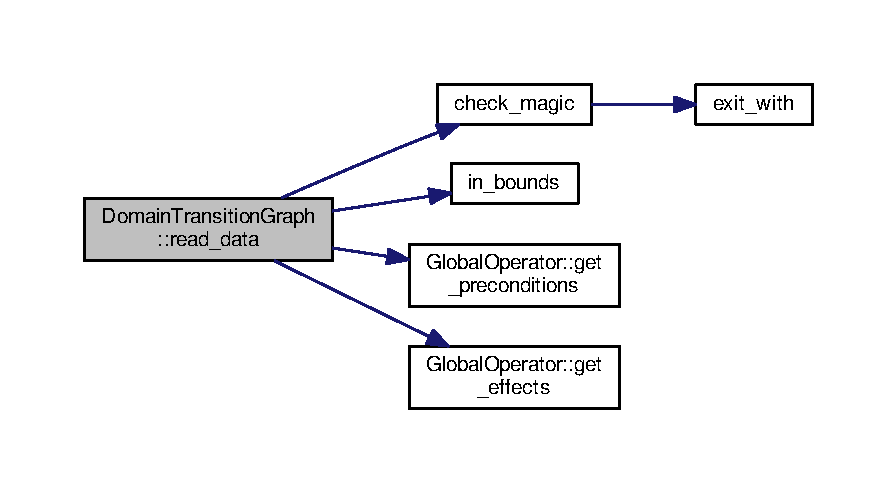
\includegraphics[width=350pt]{classDomainTransitionGraph_a80221d83ff7109b5f5b64a8851a4a075_cgraph}
\end{center}
\end{figure}




\subsection{Friends And Related Function Documentation}
\hypertarget{classDomainTransitionGraph_acb8e7e5543a9e3929bf2d038d3a30a20}{\index{Domain\-Transition\-Graph@{Domain\-Transition\-Graph}!cea\-\_\-heuristic\-::\-Context\-Enhanced\-Additive\-Heuristic@{cea\-\_\-heuristic\-::\-Context\-Enhanced\-Additive\-Heuristic}}
\index{cea\-\_\-heuristic\-::\-Context\-Enhanced\-Additive\-Heuristic@{cea\-\_\-heuristic\-::\-Context\-Enhanced\-Additive\-Heuristic}!DomainTransitionGraph@{Domain\-Transition\-Graph}}
\subsubsection[{cea\-\_\-heuristic\-::\-Context\-Enhanced\-Additive\-Heuristic}]{\setlength{\rightskip}{0pt plus 5cm}friend class {\bf cea\-\_\-heuristic\-::\-Context\-Enhanced\-Additive\-Heuristic}\hspace{0.3cm}{\ttfamily [friend]}}}\label{classDomainTransitionGraph_acb8e7e5543a9e3929bf2d038d3a30a20}
\hypertarget{classDomainTransitionGraph_af48a2cc498085d9855e0a1d95b8ee7b4}{\index{Domain\-Transition\-Graph@{Domain\-Transition\-Graph}!C\-G\-Heuristic@{C\-G\-Heuristic}}
\index{C\-G\-Heuristic@{C\-G\-Heuristic}!DomainTransitionGraph@{Domain\-Transition\-Graph}}
\subsubsection[{C\-G\-Heuristic}]{\setlength{\rightskip}{0pt plus 5cm}friend class {\bf C\-G\-Heuristic}\hspace{0.3cm}{\ttfamily [friend]}}}\label{classDomainTransitionGraph_af48a2cc498085d9855e0a1d95b8ee7b4}
\hypertarget{classDomainTransitionGraph_aa088a060547b679aea38e0bc3accf661}{\index{Domain\-Transition\-Graph@{Domain\-Transition\-Graph}!Local\-Assignment@{Local\-Assignment}}
\index{Local\-Assignment@{Local\-Assignment}!DomainTransitionGraph@{Domain\-Transition\-Graph}}
\subsubsection[{Local\-Assignment}]{\setlength{\rightskip}{0pt plus 5cm}friend struct {\bf Local\-Assignment}\hspace{0.3cm}{\ttfamily [friend]}}}\label{classDomainTransitionGraph_aa088a060547b679aea38e0bc3accf661}
\hypertarget{classDomainTransitionGraph_a111633b0408f9645dc6e3f8233f2511a}{\index{Domain\-Transition\-Graph@{Domain\-Transition\-Graph}!Value\-Node@{Value\-Node}}
\index{Value\-Node@{Value\-Node}!DomainTransitionGraph@{Domain\-Transition\-Graph}}
\subsubsection[{Value\-Node}]{\setlength{\rightskip}{0pt plus 5cm}friend struct {\bf Value\-Node}\hspace{0.3cm}{\ttfamily [friend]}}}\label{classDomainTransitionGraph_a111633b0408f9645dc6e3f8233f2511a}
\hypertarget{classDomainTransitionGraph_a14fe5a6c4d0b0fe3d17004e5a8daab2f}{\index{Domain\-Transition\-Graph@{Domain\-Transition\-Graph}!Value\-Transition@{Value\-Transition}}
\index{Value\-Transition@{Value\-Transition}!DomainTransitionGraph@{Domain\-Transition\-Graph}}
\subsubsection[{Value\-Transition}]{\setlength{\rightskip}{0pt plus 5cm}friend struct {\bf Value\-Transition}\hspace{0.3cm}{\ttfamily [friend]}}}\label{classDomainTransitionGraph_a14fe5a6c4d0b0fe3d17004e5a8daab2f}


The documentation for this class was generated from the following files\-:\begin{DoxyCompactItemize}
\item 
\hyperlink{domain__transition__graph_8h}{domain\-\_\-transition\-\_\-graph.\-h}\item 
\hyperlink{domain__transition__graph_8cc}{domain\-\_\-transition\-\_\-graph.\-cc}\end{DoxyCompactItemize}

\hypertarget{structDoubleEpsilonEquality}{\section{Double\-Epsilon\-Equality Struct Reference}
\label{structDoubleEpsilonEquality}\index{Double\-Epsilon\-Equality@{Double\-Epsilon\-Equality}}
}


{\ttfamily \#include $<$equivalence\-\_\-relation.\-h$>$}

\subsection*{Public Member Functions}
\begin{DoxyCompactItemize}
\item 
bool \hyperlink{structDoubleEpsilonEquality_adcd0ba20fb629cab6f74c72684703c4b}{operator()} (const double \&d1, const double \&d2)
\end{DoxyCompactItemize}


\subsection{Member Function Documentation}
\hypertarget{structDoubleEpsilonEquality_adcd0ba20fb629cab6f74c72684703c4b}{\index{Double\-Epsilon\-Equality@{Double\-Epsilon\-Equality}!operator()@{operator()}}
\index{operator()@{operator()}!DoubleEpsilonEquality@{Double\-Epsilon\-Equality}}
\subsubsection[{operator()}]{\setlength{\rightskip}{0pt plus 5cm}bool Double\-Epsilon\-Equality\-::operator() (
\begin{DoxyParamCaption}
\item[{const double \&}]{d1, }
\item[{const double \&}]{d2}
\end{DoxyParamCaption}
)\hspace{0.3cm}{\ttfamily [inline]}}}\label{structDoubleEpsilonEquality_adcd0ba20fb629cab6f74c72684703c4b}


The documentation for this struct was generated from the following file\-:\begin{DoxyCompactItemize}
\item 
\hyperlink{equivalence__relation_8h}{equivalence\-\_\-relation.\-h}\end{DoxyCompactItemize}

\hypertarget{classEagerSearch}{\section{Eager\-Search Class Reference}
\label{classEagerSearch}\index{Eager\-Search@{Eager\-Search}}
}


{\ttfamily \#include $<$eager\-\_\-search.\-h$>$}



Inheritance diagram for Eager\-Search\-:
\nopagebreak
\begin{figure}[H]
\begin{center}
\leavevmode
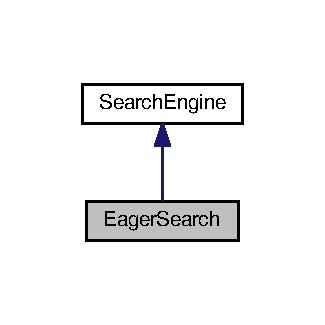
\includegraphics[width=156pt]{classEagerSearch__inherit__graph}
\end{center}
\end{figure}


Collaboration diagram for Eager\-Search\-:
\nopagebreak
\begin{figure}[H]
\begin{center}
\leavevmode
\includegraphics[width=350pt]{classEagerSearch__coll__graph}
\end{center}
\end{figure}
\subsection*{Public Member Functions}
\begin{DoxyCompactItemize}
\item 
\hyperlink{classEagerSearch_a3c83aaaa9c15bd7e60cb239d2c329704}{Eager\-Search} (const \hyperlink{classOptions}{Options} \&opts)
\item 
virtual \hyperlink{classEagerSearch_af675ad5c78c5cfa73b464cf25e91e4e4}{$\sim$\-Eager\-Search} ()=default
\item 
virtual void \hyperlink{classEagerSearch_a96bb41d45681b398293fc53b43b73782}{print\-\_\-statistics} () const override
\item 
void \hyperlink{classEagerSearch_ade1c6231195370eeabe0d8a25998a81d}{dump\-\_\-search\-\_\-space} () const 
\end{DoxyCompactItemize}
\subsection*{Protected Member Functions}
\begin{DoxyCompactItemize}
\item 
virtual void \hyperlink{classEagerSearch_ad2a84b79cbb0db13f18d9e32996303e0}{initialize} () override
\item 
virtual \hyperlink{search__engine_8h_a366b21ffe1b22f34ec2fa8f101b979f3}{Search\-Status} \hyperlink{classEagerSearch_a579812c68f5321a6eb9e6fe0da59e14c}{step} () override
\end{DoxyCompactItemize}
\subsection*{Additional Inherited Members}


\subsection{Constructor \& Destructor Documentation}
\hypertarget{classEagerSearch_a3c83aaaa9c15bd7e60cb239d2c329704}{\index{Eager\-Search@{Eager\-Search}!Eager\-Search@{Eager\-Search}}
\index{Eager\-Search@{Eager\-Search}!EagerSearch@{Eager\-Search}}
\subsubsection[{Eager\-Search}]{\setlength{\rightskip}{0pt plus 5cm}Eager\-Search\-::\-Eager\-Search (
\begin{DoxyParamCaption}
\item[{const {\bf Options} \&}]{opts}
\end{DoxyParamCaption}
)\hspace{0.3cm}{\ttfamily [explicit]}}}\label{classEagerSearch_a3c83aaaa9c15bd7e60cb239d2c329704}
\hypertarget{classEagerSearch_af675ad5c78c5cfa73b464cf25e91e4e4}{\index{Eager\-Search@{Eager\-Search}!$\sim$\-Eager\-Search@{$\sim$\-Eager\-Search}}
\index{$\sim$\-Eager\-Search@{$\sim$\-Eager\-Search}!EagerSearch@{Eager\-Search}}
\subsubsection[{$\sim$\-Eager\-Search}]{\setlength{\rightskip}{0pt plus 5cm}virtual Eager\-Search\-::$\sim$\-Eager\-Search (
\begin{DoxyParamCaption}
{}
\end{DoxyParamCaption}
)\hspace{0.3cm}{\ttfamily [virtual]}, {\ttfamily [default]}}}\label{classEagerSearch_af675ad5c78c5cfa73b464cf25e91e4e4}


\subsection{Member Function Documentation}
\hypertarget{classEagerSearch_ade1c6231195370eeabe0d8a25998a81d}{\index{Eager\-Search@{Eager\-Search}!dump\-\_\-search\-\_\-space@{dump\-\_\-search\-\_\-space}}
\index{dump\-\_\-search\-\_\-space@{dump\-\_\-search\-\_\-space}!EagerSearch@{Eager\-Search}}
\subsubsection[{dump\-\_\-search\-\_\-space}]{\setlength{\rightskip}{0pt plus 5cm}void Eager\-Search\-::dump\-\_\-search\-\_\-space (
\begin{DoxyParamCaption}
{}
\end{DoxyParamCaption}
) const}}\label{classEagerSearch_ade1c6231195370eeabe0d8a25998a81d}


Here is the call graph for this function\-:
\nopagebreak
\begin{figure}[H]
\begin{center}
\leavevmode
\includegraphics[width=350pt]{classEagerSearch_ade1c6231195370eeabe0d8a25998a81d_cgraph}
\end{center}
\end{figure}


\hypertarget{classEagerSearch_ad2a84b79cbb0db13f18d9e32996303e0}{\index{Eager\-Search@{Eager\-Search}!initialize@{initialize}}
\index{initialize@{initialize}!EagerSearch@{Eager\-Search}}
\subsubsection[{initialize}]{\setlength{\rightskip}{0pt plus 5cm}void Eager\-Search\-::initialize (
\begin{DoxyParamCaption}
{}
\end{DoxyParamCaption}
)\hspace{0.3cm}{\ttfamily [override]}, {\ttfamily [protected]}, {\ttfamily [virtual]}}}\label{classEagerSearch_ad2a84b79cbb0db13f18d9e32996303e0}


Reimplemented from \hyperlink{classSearchEngine_a72ae04f864fc906a5caa1d17bbbd3e95}{Search\-Engine}.



Here is the call graph for this function\-:
\nopagebreak
\begin{figure}[H]
\begin{center}
\leavevmode
\includegraphics[width=350pt]{classEagerSearch_ad2a84b79cbb0db13f18d9e32996303e0_cgraph}
\end{center}
\end{figure}


\hypertarget{classEagerSearch_a96bb41d45681b398293fc53b43b73782}{\index{Eager\-Search@{Eager\-Search}!print\-\_\-statistics@{print\-\_\-statistics}}
\index{print\-\_\-statistics@{print\-\_\-statistics}!EagerSearch@{Eager\-Search}}
\subsubsection[{print\-\_\-statistics}]{\setlength{\rightskip}{0pt plus 5cm}void Eager\-Search\-::print\-\_\-statistics (
\begin{DoxyParamCaption}
{}
\end{DoxyParamCaption}
) const\hspace{0.3cm}{\ttfamily [override]}, {\ttfamily [virtual]}}}\label{classEagerSearch_a96bb41d45681b398293fc53b43b73782}


Reimplemented from \hyperlink{classSearchEngine_a237e4e74b03bc1e1f777e91d98e62490}{Search\-Engine}.



Here is the call graph for this function\-:
\nopagebreak
\begin{figure}[H]
\begin{center}
\leavevmode
\includegraphics[width=350pt]{classEagerSearch_a96bb41d45681b398293fc53b43b73782_cgraph}
\end{center}
\end{figure}


\hypertarget{classEagerSearch_a579812c68f5321a6eb9e6fe0da59e14c}{\index{Eager\-Search@{Eager\-Search}!step@{step}}
\index{step@{step}!EagerSearch@{Eager\-Search}}
\subsubsection[{step}]{\setlength{\rightskip}{0pt plus 5cm}{\bf Search\-Status} Eager\-Search\-::step (
\begin{DoxyParamCaption}
{}
\end{DoxyParamCaption}
)\hspace{0.3cm}{\ttfamily [override]}, {\ttfamily [protected]}, {\ttfamily [virtual]}}}\label{classEagerSearch_a579812c68f5321a6eb9e6fe0da59e14c}


Implements \hyperlink{classSearchEngine_a2c003ac4636fd1442fd2d4eb8db5ab8d}{Search\-Engine}.



Here is the call graph for this function\-:
\nopagebreak
\begin{figure}[H]
\begin{center}
\leavevmode
\includegraphics[height=550pt]{classEagerSearch_a579812c68f5321a6eb9e6fe0da59e14c_cgraph}
\end{center}
\end{figure}




The documentation for this class was generated from the following files\-:\begin{DoxyCompactItemize}
\item 
\hyperlink{eager__search_8h}{eager\-\_\-search.\-h}\item 
\hyperlink{eager__search_8cc}{eager\-\_\-search.\-cc}\end{DoxyCompactItemize}

\hypertarget{classEffectConditionsProxy}{\section{Effect\-Conditions\-Proxy Class Reference}
\label{classEffectConditionsProxy}\index{Effect\-Conditions\-Proxy@{Effect\-Conditions\-Proxy}}
}


{\ttfamily \#include $<$task\-\_\-proxy.\-h$>$}



Inheritance diagram for Effect\-Conditions\-Proxy\-:
\nopagebreak
\begin{figure}[H]
\begin{center}
\leavevmode
\includegraphics[width=194pt]{classEffectConditionsProxy__inherit__graph}
\end{center}
\end{figure}


Collaboration diagram for Effect\-Conditions\-Proxy\-:
\nopagebreak
\begin{figure}[H]
\begin{center}
\leavevmode
\includegraphics[width=194pt]{classEffectConditionsProxy__coll__graph}
\end{center}
\end{figure}
\subsection*{Public Member Functions}
\begin{DoxyCompactItemize}
\item 
\hyperlink{classEffectConditionsProxy_a25b9e1d6b6683e4d564a2ae0df90f39b}{Effect\-Conditions\-Proxy} (const \hyperlink{classAbstractTask}{Abstract\-Task} \&\hyperlink{classConditionsProxy_a8e8c904bd5dc370a7239ec7495dc0dfe}{task}, int op\-\_\-index, int eff\-\_\-index, bool is\-\_\-axiom)
\item 
\hyperlink{classEffectConditionsProxy_a0836d4d793b2138ad1dac4d328f4345a}{$\sim$\-Effect\-Conditions\-Proxy} ()=default
\item 
std\-::size\-\_\-t \hyperlink{classEffectConditionsProxy_af447849d62079e622be08a68df7dab14}{size} () const override
\item 
\hyperlink{classFactProxy}{Fact\-Proxy} \hyperlink{classEffectConditionsProxy_a9f41ffe872d125b643591f050e8ca69a}{operator\mbox{[}$\,$\mbox{]}} (std\-::size\-\_\-t index) const override
\end{DoxyCompactItemize}
\subsection*{Additional Inherited Members}


\subsection{Constructor \& Destructor Documentation}
\hypertarget{classEffectConditionsProxy_a25b9e1d6b6683e4d564a2ae0df90f39b}{\index{Effect\-Conditions\-Proxy@{Effect\-Conditions\-Proxy}!Effect\-Conditions\-Proxy@{Effect\-Conditions\-Proxy}}
\index{Effect\-Conditions\-Proxy@{Effect\-Conditions\-Proxy}!EffectConditionsProxy@{Effect\-Conditions\-Proxy}}
\subsubsection[{Effect\-Conditions\-Proxy}]{\setlength{\rightskip}{0pt plus 5cm}Effect\-Conditions\-Proxy\-::\-Effect\-Conditions\-Proxy (
\begin{DoxyParamCaption}
\item[{const {\bf Abstract\-Task} \&}]{task, }
\item[{int}]{op\-\_\-index, }
\item[{int}]{eff\-\_\-index, }
\item[{bool}]{is\-\_\-axiom}
\end{DoxyParamCaption}
)\hspace{0.3cm}{\ttfamily [inline]}}}\label{classEffectConditionsProxy_a25b9e1d6b6683e4d564a2ae0df90f39b}
\hypertarget{classEffectConditionsProxy_a0836d4d793b2138ad1dac4d328f4345a}{\index{Effect\-Conditions\-Proxy@{Effect\-Conditions\-Proxy}!$\sim$\-Effect\-Conditions\-Proxy@{$\sim$\-Effect\-Conditions\-Proxy}}
\index{$\sim$\-Effect\-Conditions\-Proxy@{$\sim$\-Effect\-Conditions\-Proxy}!EffectConditionsProxy@{Effect\-Conditions\-Proxy}}
\subsubsection[{$\sim$\-Effect\-Conditions\-Proxy}]{\setlength{\rightskip}{0pt plus 5cm}Effect\-Conditions\-Proxy\-::$\sim$\-Effect\-Conditions\-Proxy (
\begin{DoxyParamCaption}
{}
\end{DoxyParamCaption}
)\hspace{0.3cm}{\ttfamily [default]}}}\label{classEffectConditionsProxy_a0836d4d793b2138ad1dac4d328f4345a}


\subsection{Member Function Documentation}
\hypertarget{classEffectConditionsProxy_a9f41ffe872d125b643591f050e8ca69a}{\index{Effect\-Conditions\-Proxy@{Effect\-Conditions\-Proxy}!operator\mbox{[}$\,$\mbox{]}@{operator[]}}
\index{operator\mbox{[}$\,$\mbox{]}@{operator[]}!EffectConditionsProxy@{Effect\-Conditions\-Proxy}}
\subsubsection[{operator[]}]{\setlength{\rightskip}{0pt plus 5cm}{\bf Fact\-Proxy} Effect\-Conditions\-Proxy\-::operator\mbox{[}$\,$\mbox{]} (
\begin{DoxyParamCaption}
\item[{std\-::size\-\_\-t}]{index}
\end{DoxyParamCaption}
) const\hspace{0.3cm}{\ttfamily [inline]}, {\ttfamily [override]}, {\ttfamily [virtual]}}}\label{classEffectConditionsProxy_a9f41ffe872d125b643591f050e8ca69a}


Implements \hyperlink{classConditionsProxy_a558d807927b992bad3728268b7e8a533}{Conditions\-Proxy}.



Here is the call graph for this function\-:
\nopagebreak
\begin{figure}[H]
\begin{center}
\leavevmode
\includegraphics[width=350pt]{classEffectConditionsProxy_a9f41ffe872d125b643591f050e8ca69a_cgraph}
\end{center}
\end{figure}


\hypertarget{classEffectConditionsProxy_af447849d62079e622be08a68df7dab14}{\index{Effect\-Conditions\-Proxy@{Effect\-Conditions\-Proxy}!size@{size}}
\index{size@{size}!EffectConditionsProxy@{Effect\-Conditions\-Proxy}}
\subsubsection[{size}]{\setlength{\rightskip}{0pt plus 5cm}std\-::size\-\_\-t Effect\-Conditions\-Proxy\-::size (
\begin{DoxyParamCaption}
{}
\end{DoxyParamCaption}
) const\hspace{0.3cm}{\ttfamily [inline]}, {\ttfamily [override]}, {\ttfamily [virtual]}}}\label{classEffectConditionsProxy_af447849d62079e622be08a68df7dab14}


Implements \hyperlink{classConditionsProxy_af0710776571971659082f0140e4cdba3}{Conditions\-Proxy}.



Here is the call graph for this function\-:
\nopagebreak
\begin{figure}[H]
\begin{center}
\leavevmode
\includegraphics[width=350pt]{classEffectConditionsProxy_af447849d62079e622be08a68df7dab14_cgraph}
\end{center}
\end{figure}




The documentation for this class was generated from the following file\-:\begin{DoxyCompactItemize}
\item 
\hyperlink{task__proxy_8h}{task\-\_\-proxy.\-h}\end{DoxyCompactItemize}

\hypertarget{classEffectProxy}{\section{Effect\-Proxy Class Reference}
\label{classEffectProxy}\index{Effect\-Proxy@{Effect\-Proxy}}
}


{\ttfamily \#include $<$task\-\_\-proxy.\-h$>$}

\subsection*{Public Member Functions}
\begin{DoxyCompactItemize}
\item 
\hyperlink{classEffectProxy_a57ae9eff89329c42acfe20093974f2a0}{Effect\-Proxy} (const \hyperlink{classAbstractTask}{Abstract\-Task} \&task, int op\-\_\-index, int eff\-\_\-index, bool is\-\_\-axiom)
\item 
\hyperlink{classEffectProxy_a79af0d03c64d2ccf24fae03a01e5823f}{$\sim$\-Effect\-Proxy} ()=default
\item 
\hyperlink{classEffectConditionsProxy}{Effect\-Conditions\-Proxy} \hyperlink{classEffectProxy_aaf1a977be327948a5247a9cf41ea0040}{get\-\_\-conditions} () const 
\item 
\hyperlink{classFactProxy}{Fact\-Proxy} \hyperlink{classEffectProxy_acd22da8c2db417fb7286e410eb354eb6}{get\-\_\-fact} () const 
\end{DoxyCompactItemize}


\subsection{Constructor \& Destructor Documentation}
\hypertarget{classEffectProxy_a57ae9eff89329c42acfe20093974f2a0}{\index{Effect\-Proxy@{Effect\-Proxy}!Effect\-Proxy@{Effect\-Proxy}}
\index{Effect\-Proxy@{Effect\-Proxy}!EffectProxy@{Effect\-Proxy}}
\subsubsection[{Effect\-Proxy}]{\setlength{\rightskip}{0pt plus 5cm}Effect\-Proxy\-::\-Effect\-Proxy (
\begin{DoxyParamCaption}
\item[{const {\bf Abstract\-Task} \&}]{task, }
\item[{int}]{op\-\_\-index, }
\item[{int}]{eff\-\_\-index, }
\item[{bool}]{is\-\_\-axiom}
\end{DoxyParamCaption}
)\hspace{0.3cm}{\ttfamily [inline]}}}\label{classEffectProxy_a57ae9eff89329c42acfe20093974f2a0}
\hypertarget{classEffectProxy_a79af0d03c64d2ccf24fae03a01e5823f}{\index{Effect\-Proxy@{Effect\-Proxy}!$\sim$\-Effect\-Proxy@{$\sim$\-Effect\-Proxy}}
\index{$\sim$\-Effect\-Proxy@{$\sim$\-Effect\-Proxy}!EffectProxy@{Effect\-Proxy}}
\subsubsection[{$\sim$\-Effect\-Proxy}]{\setlength{\rightskip}{0pt plus 5cm}Effect\-Proxy\-::$\sim$\-Effect\-Proxy (
\begin{DoxyParamCaption}
{}
\end{DoxyParamCaption}
)\hspace{0.3cm}{\ttfamily [default]}}}\label{classEffectProxy_a79af0d03c64d2ccf24fae03a01e5823f}


\subsection{Member Function Documentation}
\hypertarget{classEffectProxy_aaf1a977be327948a5247a9cf41ea0040}{\index{Effect\-Proxy@{Effect\-Proxy}!get\-\_\-conditions@{get\-\_\-conditions}}
\index{get\-\_\-conditions@{get\-\_\-conditions}!EffectProxy@{Effect\-Proxy}}
\subsubsection[{get\-\_\-conditions}]{\setlength{\rightskip}{0pt plus 5cm}{\bf Effect\-Conditions\-Proxy} Effect\-Proxy\-::get\-\_\-conditions (
\begin{DoxyParamCaption}
{}
\end{DoxyParamCaption}
) const\hspace{0.3cm}{\ttfamily [inline]}}}\label{classEffectProxy_aaf1a977be327948a5247a9cf41ea0040}
\hypertarget{classEffectProxy_acd22da8c2db417fb7286e410eb354eb6}{\index{Effect\-Proxy@{Effect\-Proxy}!get\-\_\-fact@{get\-\_\-fact}}
\index{get\-\_\-fact@{get\-\_\-fact}!EffectProxy@{Effect\-Proxy}}
\subsubsection[{get\-\_\-fact}]{\setlength{\rightskip}{0pt plus 5cm}{\bf Fact\-Proxy} Effect\-Proxy\-::get\-\_\-fact (
\begin{DoxyParamCaption}
{}
\end{DoxyParamCaption}
) const\hspace{0.3cm}{\ttfamily [inline]}}}\label{classEffectProxy_acd22da8c2db417fb7286e410eb354eb6}


Here is the call graph for this function\-:
\nopagebreak
\begin{figure}[H]
\begin{center}
\leavevmode
\includegraphics[width=350pt]{classEffectProxy_acd22da8c2db417fb7286e410eb354eb6_cgraph}
\end{center}
\end{figure}




The documentation for this class was generated from the following file\-:\begin{DoxyCompactItemize}
\item 
\hyperlink{task__proxy_8h}{task\-\_\-proxy.\-h}\end{DoxyCompactItemize}

\hypertarget{classEffectsProxy}{\section{Effects\-Proxy Class Reference}
\label{classEffectsProxy}\index{Effects\-Proxy@{Effects\-Proxy}}
}


{\ttfamily \#include $<$task\-\_\-proxy.\-h$>$}

\subsection*{Public Types}
\begin{DoxyCompactItemize}
\item 
using \hyperlink{classEffectsProxy_a7cafa2192ee2e829a7479129e871e7eb}{Item\-Type} = \hyperlink{classEffectProxy}{Effect\-Proxy}
\end{DoxyCompactItemize}
\subsection*{Public Member Functions}
\begin{DoxyCompactItemize}
\item 
\hyperlink{classEffectsProxy_a12d9791a9bd90df7f0fb1efb1c800782}{Effects\-Proxy} (const \hyperlink{classAbstractTask}{Abstract\-Task} \&task, int op\-\_\-index, bool is\-\_\-axiom)
\item 
\hyperlink{classEffectsProxy_a55c03d1012518ca3ac7c55757c3d66dc}{$\sim$\-Effects\-Proxy} ()=default
\item 
std\-::size\-\_\-t \hyperlink{classEffectsProxy_ab153e05e58aef798690cd76d565aaaf9}{size} () const 
\item 
\hyperlink{classEffectProxy}{Effect\-Proxy} \hyperlink{classEffectsProxy_a462603bb0a8f8ca8b6bbfc6d4517f6a9}{operator\mbox{[}$\,$\mbox{]}} (std\-::size\-\_\-t eff\-\_\-index) const 
\end{DoxyCompactItemize}


\subsection{Member Typedef Documentation}
\hypertarget{classEffectsProxy_a7cafa2192ee2e829a7479129e871e7eb}{\index{Effects\-Proxy@{Effects\-Proxy}!Item\-Type@{Item\-Type}}
\index{Item\-Type@{Item\-Type}!EffectsProxy@{Effects\-Proxy}}
\subsubsection[{Item\-Type}]{\setlength{\rightskip}{0pt plus 5cm}using {\bf Effects\-Proxy\-::\-Item\-Type} =  {\bf Effect\-Proxy}}}\label{classEffectsProxy_a7cafa2192ee2e829a7479129e871e7eb}


\subsection{Constructor \& Destructor Documentation}
\hypertarget{classEffectsProxy_a12d9791a9bd90df7f0fb1efb1c800782}{\index{Effects\-Proxy@{Effects\-Proxy}!Effects\-Proxy@{Effects\-Proxy}}
\index{Effects\-Proxy@{Effects\-Proxy}!EffectsProxy@{Effects\-Proxy}}
\subsubsection[{Effects\-Proxy}]{\setlength{\rightskip}{0pt plus 5cm}Effects\-Proxy\-::\-Effects\-Proxy (
\begin{DoxyParamCaption}
\item[{const {\bf Abstract\-Task} \&}]{task, }
\item[{int}]{op\-\_\-index, }
\item[{bool}]{is\-\_\-axiom}
\end{DoxyParamCaption}
)\hspace{0.3cm}{\ttfamily [inline]}}}\label{classEffectsProxy_a12d9791a9bd90df7f0fb1efb1c800782}
\hypertarget{classEffectsProxy_a55c03d1012518ca3ac7c55757c3d66dc}{\index{Effects\-Proxy@{Effects\-Proxy}!$\sim$\-Effects\-Proxy@{$\sim$\-Effects\-Proxy}}
\index{$\sim$\-Effects\-Proxy@{$\sim$\-Effects\-Proxy}!EffectsProxy@{Effects\-Proxy}}
\subsubsection[{$\sim$\-Effects\-Proxy}]{\setlength{\rightskip}{0pt plus 5cm}Effects\-Proxy\-::$\sim$\-Effects\-Proxy (
\begin{DoxyParamCaption}
{}
\end{DoxyParamCaption}
)\hspace{0.3cm}{\ttfamily [default]}}}\label{classEffectsProxy_a55c03d1012518ca3ac7c55757c3d66dc}


\subsection{Member Function Documentation}
\hypertarget{classEffectsProxy_a462603bb0a8f8ca8b6bbfc6d4517f6a9}{\index{Effects\-Proxy@{Effects\-Proxy}!operator\mbox{[}$\,$\mbox{]}@{operator[]}}
\index{operator\mbox{[}$\,$\mbox{]}@{operator[]}!EffectsProxy@{Effects\-Proxy}}
\subsubsection[{operator[]}]{\setlength{\rightskip}{0pt plus 5cm}{\bf Effect\-Proxy} Effects\-Proxy\-::operator\mbox{[}$\,$\mbox{]} (
\begin{DoxyParamCaption}
\item[{std\-::size\-\_\-t}]{eff\-\_\-index}
\end{DoxyParamCaption}
) const\hspace{0.3cm}{\ttfamily [inline]}}}\label{classEffectsProxy_a462603bb0a8f8ca8b6bbfc6d4517f6a9}


Here is the call graph for this function\-:
\nopagebreak
\begin{figure}[H]
\begin{center}
\leavevmode
\includegraphics[width=350pt]{classEffectsProxy_a462603bb0a8f8ca8b6bbfc6d4517f6a9_cgraph}
\end{center}
\end{figure}


\hypertarget{classEffectsProxy_ab153e05e58aef798690cd76d565aaaf9}{\index{Effects\-Proxy@{Effects\-Proxy}!size@{size}}
\index{size@{size}!EffectsProxy@{Effects\-Proxy}}
\subsubsection[{size}]{\setlength{\rightskip}{0pt plus 5cm}std\-::size\-\_\-t Effects\-Proxy\-::size (
\begin{DoxyParamCaption}
{}
\end{DoxyParamCaption}
) const\hspace{0.3cm}{\ttfamily [inline]}}}\label{classEffectsProxy_ab153e05e58aef798690cd76d565aaaf9}


Here is the call graph for this function\-:
\nopagebreak
\begin{figure}[H]
\begin{center}
\leavevmode
\includegraphics[width=334pt]{classEffectsProxy_ab153e05e58aef798690cd76d565aaaf9_cgraph}
\end{center}
\end{figure}




The documentation for this class was generated from the following file\-:\begin{DoxyCompactItemize}
\item 
\hyperlink{task__proxy_8h}{task\-\_\-proxy.\-h}\end{DoxyCompactItemize}

\hypertarget{classEnforcedHillClimbingSearch}{\section{Enforced\-Hill\-Climbing\-Search Class Reference}
\label{classEnforcedHillClimbingSearch}\index{Enforced\-Hill\-Climbing\-Search@{Enforced\-Hill\-Climbing\-Search}}
}


{\ttfamily \#include $<$enforced\-\_\-hill\-\_\-climbing\-\_\-search.\-h$>$}



Inheritance diagram for Enforced\-Hill\-Climbing\-Search\-:
\nopagebreak
\begin{figure}[H]
\begin{center}
\leavevmode
\includegraphics[width=218pt]{classEnforcedHillClimbingSearch__inherit__graph}
\end{center}
\end{figure}


Collaboration diagram for Enforced\-Hill\-Climbing\-Search\-:
\nopagebreak
\begin{figure}[H]
\begin{center}
\leavevmode
\includegraphics[width=350pt]{classEnforcedHillClimbingSearch__coll__graph}
\end{center}
\end{figure}
\subsection*{Public Member Functions}
\begin{DoxyCompactItemize}
\item 
\hyperlink{classEnforcedHillClimbingSearch_ab1a9588921fbc54c2201d58e4c4630dd}{Enforced\-Hill\-Climbing\-Search} (const \hyperlink{classOptions}{Options} \&opts)
\item 
virtual \hyperlink{classEnforcedHillClimbingSearch_a5586307df39c671bb80ce52b1ebeff6b}{$\sim$\-Enforced\-Hill\-Climbing\-Search} () override
\item 
virtual void \hyperlink{classEnforcedHillClimbingSearch_a2b1cd0e9682f6859aef38af51b5664b4}{print\-\_\-statistics} () const override
\end{DoxyCompactItemize}
\subsection*{Protected Member Functions}
\begin{DoxyCompactItemize}
\item 
virtual void \hyperlink{classEnforcedHillClimbingSearch_a4ec8b675b4ae6813a1a4726d511ae1ed}{initialize} () override
\item 
virtual \hyperlink{search__engine_8h_a366b21ffe1b22f34ec2fa8f101b979f3}{Search\-Status} \hyperlink{classEnforcedHillClimbingSearch_a792b3c175edfe829dd67401eb1060fce}{step} () override
\end{DoxyCompactItemize}
\subsection*{Additional Inherited Members}


\subsection{Constructor \& Destructor Documentation}
\hypertarget{classEnforcedHillClimbingSearch_ab1a9588921fbc54c2201d58e4c4630dd}{\index{Enforced\-Hill\-Climbing\-Search@{Enforced\-Hill\-Climbing\-Search}!Enforced\-Hill\-Climbing\-Search@{Enforced\-Hill\-Climbing\-Search}}
\index{Enforced\-Hill\-Climbing\-Search@{Enforced\-Hill\-Climbing\-Search}!EnforcedHillClimbingSearch@{Enforced\-Hill\-Climbing\-Search}}
\subsubsection[{Enforced\-Hill\-Climbing\-Search}]{\setlength{\rightskip}{0pt plus 5cm}Enforced\-Hill\-Climbing\-Search\-::\-Enforced\-Hill\-Climbing\-Search (
\begin{DoxyParamCaption}
\item[{const {\bf Options} \&}]{opts}
\end{DoxyParamCaption}
)\hspace{0.3cm}{\ttfamily [explicit]}}}\label{classEnforcedHillClimbingSearch_ab1a9588921fbc54c2201d58e4c4630dd}
\hypertarget{classEnforcedHillClimbingSearch_a5586307df39c671bb80ce52b1ebeff6b}{\index{Enforced\-Hill\-Climbing\-Search@{Enforced\-Hill\-Climbing\-Search}!$\sim$\-Enforced\-Hill\-Climbing\-Search@{$\sim$\-Enforced\-Hill\-Climbing\-Search}}
\index{$\sim$\-Enforced\-Hill\-Climbing\-Search@{$\sim$\-Enforced\-Hill\-Climbing\-Search}!EnforcedHillClimbingSearch@{Enforced\-Hill\-Climbing\-Search}}
\subsubsection[{$\sim$\-Enforced\-Hill\-Climbing\-Search}]{\setlength{\rightskip}{0pt plus 5cm}Enforced\-Hill\-Climbing\-Search\-::$\sim$\-Enforced\-Hill\-Climbing\-Search (
\begin{DoxyParamCaption}
{}
\end{DoxyParamCaption}
)\hspace{0.3cm}{\ttfamily [override]}, {\ttfamily [virtual]}}}\label{classEnforcedHillClimbingSearch_a5586307df39c671bb80ce52b1ebeff6b}


\subsection{Member Function Documentation}
\hypertarget{classEnforcedHillClimbingSearch_a4ec8b675b4ae6813a1a4726d511ae1ed}{\index{Enforced\-Hill\-Climbing\-Search@{Enforced\-Hill\-Climbing\-Search}!initialize@{initialize}}
\index{initialize@{initialize}!EnforcedHillClimbingSearch@{Enforced\-Hill\-Climbing\-Search}}
\subsubsection[{initialize}]{\setlength{\rightskip}{0pt plus 5cm}void Enforced\-Hill\-Climbing\-Search\-::initialize (
\begin{DoxyParamCaption}
{}
\end{DoxyParamCaption}
)\hspace{0.3cm}{\ttfamily [override]}, {\ttfamily [protected]}, {\ttfamily [virtual]}}}\label{classEnforcedHillClimbingSearch_a4ec8b675b4ae6813a1a4726d511ae1ed}


Reimplemented from \hyperlink{classSearchEngine_a72ae04f864fc906a5caa1d17bbbd3e95}{Search\-Engine}.



Here is the call graph for this function\-:
\nopagebreak
\begin{figure}[H]
\begin{center}
\leavevmode
\includegraphics[width=350pt]{classEnforcedHillClimbingSearch_a4ec8b675b4ae6813a1a4726d511ae1ed_cgraph}
\end{center}
\end{figure}


\hypertarget{classEnforcedHillClimbingSearch_a2b1cd0e9682f6859aef38af51b5664b4}{\index{Enforced\-Hill\-Climbing\-Search@{Enforced\-Hill\-Climbing\-Search}!print\-\_\-statistics@{print\-\_\-statistics}}
\index{print\-\_\-statistics@{print\-\_\-statistics}!EnforcedHillClimbingSearch@{Enforced\-Hill\-Climbing\-Search}}
\subsubsection[{print\-\_\-statistics}]{\setlength{\rightskip}{0pt plus 5cm}void Enforced\-Hill\-Climbing\-Search\-::print\-\_\-statistics (
\begin{DoxyParamCaption}
{}
\end{DoxyParamCaption}
) const\hspace{0.3cm}{\ttfamily [override]}, {\ttfamily [virtual]}}}\label{classEnforcedHillClimbingSearch_a2b1cd0e9682f6859aef38af51b5664b4}


Reimplemented from \hyperlink{classSearchEngine_a237e4e74b03bc1e1f777e91d98e62490}{Search\-Engine}.



Here is the call graph for this function\-:
\nopagebreak
\begin{figure}[H]
\begin{center}
\leavevmode
\includegraphics[width=350pt]{classEnforcedHillClimbingSearch_a2b1cd0e9682f6859aef38af51b5664b4_cgraph}
\end{center}
\end{figure}


\hypertarget{classEnforcedHillClimbingSearch_a792b3c175edfe829dd67401eb1060fce}{\index{Enforced\-Hill\-Climbing\-Search@{Enforced\-Hill\-Climbing\-Search}!step@{step}}
\index{step@{step}!EnforcedHillClimbingSearch@{Enforced\-Hill\-Climbing\-Search}}
\subsubsection[{step}]{\setlength{\rightskip}{0pt plus 5cm}{\bf Search\-Status} Enforced\-Hill\-Climbing\-Search\-::step (
\begin{DoxyParamCaption}
{}
\end{DoxyParamCaption}
)\hspace{0.3cm}{\ttfamily [override]}, {\ttfamily [protected]}, {\ttfamily [virtual]}}}\label{classEnforcedHillClimbingSearch_a792b3c175edfe829dd67401eb1060fce}


Implements \hyperlink{classSearchEngine_a2c003ac4636fd1442fd2d4eb8db5ab8d}{Search\-Engine}.



Here is the call graph for this function\-:
\nopagebreak
\begin{figure}[H]
\begin{center}
\leavevmode
\includegraphics[width=350pt]{classEnforcedHillClimbingSearch_a792b3c175edfe829dd67401eb1060fce_cgraph}
\end{center}
\end{figure}




The documentation for this class was generated from the following files\-:\begin{DoxyCompactItemize}
\item 
\hyperlink{enforced__hill__climbing__search_8h}{enforced\-\_\-hill\-\_\-climbing\-\_\-search.\-h}\item 
\hyperlink{enforced__hill__climbing__search_8cc}{enforced\-\_\-hill\-\_\-climbing\-\_\-search.\-cc}\end{DoxyCompactItemize}

\hypertarget{classEquivalenceRelation}{\section{Equivalence\-Relation Class Reference}
\label{classEquivalenceRelation}\index{Equivalence\-Relation@{Equivalence\-Relation}}
}


{\ttfamily \#include $<$equivalence\-\_\-relation.\-h$>$}

\subsection*{Public Member Functions}
\begin{DoxyCompactItemize}
\item 
\hyperlink{classEquivalenceRelation_a45bcace3a45f83e087b5bfd008be7a59}{Equivalence\-Relation} (int n)
\item 
\hyperlink{classEquivalenceRelation_a93e9f1d3c5298ff40895c066565b483d}{Equivalence\-Relation} (int n, const std\-::list$<$ \hyperlink{classBlock}{Block} $>$ \&blocks\-\_\-)
\item 
\hyperlink{classEquivalenceRelation_aaab14b8174df20658035397a1a672462}{$\sim$\-Equivalence\-Relation} ()
\item 
int \hyperlink{classEquivalenceRelation_a4b44f31d6d19280b6fe6f192d649572e}{get\-\_\-num\-\_\-elements} () const 
\item 
int \hyperlink{classEquivalenceRelation_af2437c19b12e284d7703bb28ff6fcc89}{get\-\_\-num\-\_\-explicit\-\_\-elements} () const 
\item 
int \hyperlink{classEquivalenceRelation_a29c0989de637b4b6ba8ca585fe94e3a4}{get\-\_\-num\-\_\-blocks} () const 
\item 
int \hyperlink{classEquivalenceRelation_aa189e7e375b1211d3445f5b2f268c832}{get\-\_\-num\-\_\-explicit\-\_\-blocks} () const 
\item 
\hyperlink{equivalence__relation_8h_a12e817b65a28b802e85b48c8b600c4a5}{Block\-List\-Const\-Iter} \hyperlink{classEquivalenceRelation_a3da008a451c9d93b6f1263a6c1fcfa76}{begin} () const 
\item 
\hyperlink{equivalence__relation_8h_a12e817b65a28b802e85b48c8b600c4a5}{Block\-List\-Const\-Iter} \hyperlink{classEquivalenceRelation_a933dfe467eb51a2d1bdeb7171910ac06}{end} () const 
\item 
void \hyperlink{classEquivalenceRelation_a998178b75f14d38f2566be8de124ef70}{refine} (const \hyperlink{classEquivalenceRelation}{Equivalence\-Relation} \&other)
\item 
void \hyperlink{classEquivalenceRelation_ad04cdc09efd376f65e984fd39780c59c}{refine} (\hyperlink{equivalence__relation_8h_adcd1a68c6846e41421e3868fd40bdd81}{Element\-List\-Const\-Iter} block\-\_\-\-X\-\_\-begin, \hyperlink{equivalence__relation_8h_adcd1a68c6846e41421e3868fd40bdd81}{Element\-List\-Const\-Iter} block\-\_\-\-X\-\_\-end)
\end{DoxyCompactItemize}
\subsection*{Static Public Member Functions}
\begin{DoxyCompactItemize}
\item 
{\footnotesize template$<$class T $>$ }\\static \hyperlink{classEquivalenceRelation}{Equivalence\-Relation} $\ast$ \hyperlink{classEquivalenceRelation_af058c58f4f2d6c7825500ad217b37125}{from\-\_\-annotated\-\_\-elements} (int n, std\-::vector$<$ std\-::pair$<$ T, int $>$ $>$ \&annotated\-\_\-elements)
\item 
{\footnotesize template$<$class T , class Equal $>$ }\\static \hyperlink{classEquivalenceRelation}{Equivalence\-Relation} $\ast$ \hyperlink{classEquivalenceRelation_af48b8e6a749b47b975a917cf6bafc1e5}{from\-\_\-annotated\-\_\-elements} (int n, std\-::vector$<$ std\-::pair$<$ T, int $>$ $>$ \&annotated\-\_\-elements)
\end{DoxyCompactItemize}


\subsection{Constructor \& Destructor Documentation}
\hypertarget{classEquivalenceRelation_a45bcace3a45f83e087b5bfd008be7a59}{\index{Equivalence\-Relation@{Equivalence\-Relation}!Equivalence\-Relation@{Equivalence\-Relation}}
\index{Equivalence\-Relation@{Equivalence\-Relation}!EquivalenceRelation@{Equivalence\-Relation}}
\subsubsection[{Equivalence\-Relation}]{\setlength{\rightskip}{0pt plus 5cm}Equivalence\-Relation\-::\-Equivalence\-Relation (
\begin{DoxyParamCaption}
\item[{int}]{n}
\end{DoxyParamCaption}
)}}\label{classEquivalenceRelation_a45bcace3a45f83e087b5bfd008be7a59}
\hypertarget{classEquivalenceRelation_a93e9f1d3c5298ff40895c066565b483d}{\index{Equivalence\-Relation@{Equivalence\-Relation}!Equivalence\-Relation@{Equivalence\-Relation}}
\index{Equivalence\-Relation@{Equivalence\-Relation}!EquivalenceRelation@{Equivalence\-Relation}}
\subsubsection[{Equivalence\-Relation}]{\setlength{\rightskip}{0pt plus 5cm}Equivalence\-Relation\-::\-Equivalence\-Relation (
\begin{DoxyParamCaption}
\item[{int}]{n, }
\item[{const std\-::list$<$ {\bf Block} $>$ \&}]{blocks\-\_\-}
\end{DoxyParamCaption}
)}}\label{classEquivalenceRelation_a93e9f1d3c5298ff40895c066565b483d}
\hypertarget{classEquivalenceRelation_aaab14b8174df20658035397a1a672462}{\index{Equivalence\-Relation@{Equivalence\-Relation}!$\sim$\-Equivalence\-Relation@{$\sim$\-Equivalence\-Relation}}
\index{$\sim$\-Equivalence\-Relation@{$\sim$\-Equivalence\-Relation}!EquivalenceRelation@{Equivalence\-Relation}}
\subsubsection[{$\sim$\-Equivalence\-Relation}]{\setlength{\rightskip}{0pt plus 5cm}Equivalence\-Relation\-::$\sim$\-Equivalence\-Relation (
\begin{DoxyParamCaption}
{}
\end{DoxyParamCaption}
)}}\label{classEquivalenceRelation_aaab14b8174df20658035397a1a672462}


\subsection{Member Function Documentation}
\hypertarget{classEquivalenceRelation_a3da008a451c9d93b6f1263a6c1fcfa76}{\index{Equivalence\-Relation@{Equivalence\-Relation}!begin@{begin}}
\index{begin@{begin}!EquivalenceRelation@{Equivalence\-Relation}}
\subsubsection[{begin}]{\setlength{\rightskip}{0pt plus 5cm}{\bf Block\-List\-Const\-Iter} Equivalence\-Relation\-::begin (
\begin{DoxyParamCaption}
{}
\end{DoxyParamCaption}
) const\hspace{0.3cm}{\ttfamily [inline]}}}\label{classEquivalenceRelation_a3da008a451c9d93b6f1263a6c1fcfa76}
\hypertarget{classEquivalenceRelation_a933dfe467eb51a2d1bdeb7171910ac06}{\index{Equivalence\-Relation@{Equivalence\-Relation}!end@{end}}
\index{end@{end}!EquivalenceRelation@{Equivalence\-Relation}}
\subsubsection[{end}]{\setlength{\rightskip}{0pt plus 5cm}{\bf Block\-List\-Const\-Iter} Equivalence\-Relation\-::end (
\begin{DoxyParamCaption}
{}
\end{DoxyParamCaption}
) const\hspace{0.3cm}{\ttfamily [inline]}}}\label{classEquivalenceRelation_a933dfe467eb51a2d1bdeb7171910ac06}
\hypertarget{classEquivalenceRelation_af058c58f4f2d6c7825500ad217b37125}{\index{Equivalence\-Relation@{Equivalence\-Relation}!from\-\_\-annotated\-\_\-elements@{from\-\_\-annotated\-\_\-elements}}
\index{from\-\_\-annotated\-\_\-elements@{from\-\_\-annotated\-\_\-elements}!EquivalenceRelation@{Equivalence\-Relation}}
\subsubsection[{from\-\_\-annotated\-\_\-elements}]{\setlength{\rightskip}{0pt plus 5cm}template$<$class T $>$ {\bf Equivalence\-Relation} $\ast$ Equivalence\-Relation\-::from\-\_\-annotated\-\_\-elements (
\begin{DoxyParamCaption}
\item[{int}]{n, }
\item[{std\-::vector$<$ std\-::pair$<$ T, int $>$ $>$ \&}]{annotated\-\_\-elements}
\end{DoxyParamCaption}
)\hspace{0.3cm}{\ttfamily [static]}}}\label{classEquivalenceRelation_af058c58f4f2d6c7825500ad217b37125}
\hypertarget{classEquivalenceRelation_af48b8e6a749b47b975a917cf6bafc1e5}{\index{Equivalence\-Relation@{Equivalence\-Relation}!from\-\_\-annotated\-\_\-elements@{from\-\_\-annotated\-\_\-elements}}
\index{from\-\_\-annotated\-\_\-elements@{from\-\_\-annotated\-\_\-elements}!EquivalenceRelation@{Equivalence\-Relation}}
\subsubsection[{from\-\_\-annotated\-\_\-elements}]{\setlength{\rightskip}{0pt plus 5cm}template$<$class T , class Equal $>$ {\bf Equivalence\-Relation} $\ast$ Equivalence\-Relation\-::from\-\_\-annotated\-\_\-elements (
\begin{DoxyParamCaption}
\item[{int}]{n, }
\item[{std\-::vector$<$ std\-::pair$<$ T, int $>$ $>$ \&}]{annotated\-\_\-elements}
\end{DoxyParamCaption}
)\hspace{0.3cm}{\ttfamily [static]}}}\label{classEquivalenceRelation_af48b8e6a749b47b975a917cf6bafc1e5}


Here is the call graph for this function\-:
\nopagebreak
\begin{figure}[H]
\begin{center}
\leavevmode
\includegraphics[width=350pt]{classEquivalenceRelation_af48b8e6a749b47b975a917cf6bafc1e5_cgraph}
\end{center}
\end{figure}


\hypertarget{classEquivalenceRelation_a29c0989de637b4b6ba8ca585fe94e3a4}{\index{Equivalence\-Relation@{Equivalence\-Relation}!get\-\_\-num\-\_\-blocks@{get\-\_\-num\-\_\-blocks}}
\index{get\-\_\-num\-\_\-blocks@{get\-\_\-num\-\_\-blocks}!EquivalenceRelation@{Equivalence\-Relation}}
\subsubsection[{get\-\_\-num\-\_\-blocks}]{\setlength{\rightskip}{0pt plus 5cm}int Equivalence\-Relation\-::get\-\_\-num\-\_\-blocks (
\begin{DoxyParamCaption}
{}
\end{DoxyParamCaption}
) const}}\label{classEquivalenceRelation_a29c0989de637b4b6ba8ca585fe94e3a4}


Here is the call graph for this function\-:
\nopagebreak
\begin{figure}[H]
\begin{center}
\leavevmode
\includegraphics[width=350pt]{classEquivalenceRelation_a29c0989de637b4b6ba8ca585fe94e3a4_cgraph}
\end{center}
\end{figure}


\hypertarget{classEquivalenceRelation_a4b44f31d6d19280b6fe6f192d649572e}{\index{Equivalence\-Relation@{Equivalence\-Relation}!get\-\_\-num\-\_\-elements@{get\-\_\-num\-\_\-elements}}
\index{get\-\_\-num\-\_\-elements@{get\-\_\-num\-\_\-elements}!EquivalenceRelation@{Equivalence\-Relation}}
\subsubsection[{get\-\_\-num\-\_\-elements}]{\setlength{\rightskip}{0pt plus 5cm}int Equivalence\-Relation\-::get\-\_\-num\-\_\-elements (
\begin{DoxyParamCaption}
{}
\end{DoxyParamCaption}
) const}}\label{classEquivalenceRelation_a4b44f31d6d19280b6fe6f192d649572e}
\hypertarget{classEquivalenceRelation_aa189e7e375b1211d3445f5b2f268c832}{\index{Equivalence\-Relation@{Equivalence\-Relation}!get\-\_\-num\-\_\-explicit\-\_\-blocks@{get\-\_\-num\-\_\-explicit\-\_\-blocks}}
\index{get\-\_\-num\-\_\-explicit\-\_\-blocks@{get\-\_\-num\-\_\-explicit\-\_\-blocks}!EquivalenceRelation@{Equivalence\-Relation}}
\subsubsection[{get\-\_\-num\-\_\-explicit\-\_\-blocks}]{\setlength{\rightskip}{0pt plus 5cm}int Equivalence\-Relation\-::get\-\_\-num\-\_\-explicit\-\_\-blocks (
\begin{DoxyParamCaption}
{}
\end{DoxyParamCaption}
) const}}\label{classEquivalenceRelation_aa189e7e375b1211d3445f5b2f268c832}
\hypertarget{classEquivalenceRelation_af2437c19b12e284d7703bb28ff6fcc89}{\index{Equivalence\-Relation@{Equivalence\-Relation}!get\-\_\-num\-\_\-explicit\-\_\-elements@{get\-\_\-num\-\_\-explicit\-\_\-elements}}
\index{get\-\_\-num\-\_\-explicit\-\_\-elements@{get\-\_\-num\-\_\-explicit\-\_\-elements}!EquivalenceRelation@{Equivalence\-Relation}}
\subsubsection[{get\-\_\-num\-\_\-explicit\-\_\-elements}]{\setlength{\rightskip}{0pt plus 5cm}int Equivalence\-Relation\-::get\-\_\-num\-\_\-explicit\-\_\-elements (
\begin{DoxyParamCaption}
{}
\end{DoxyParamCaption}
) const}}\label{classEquivalenceRelation_af2437c19b12e284d7703bb28ff6fcc89}
\hypertarget{classEquivalenceRelation_a998178b75f14d38f2566be8de124ef70}{\index{Equivalence\-Relation@{Equivalence\-Relation}!refine@{refine}}
\index{refine@{refine}!EquivalenceRelation@{Equivalence\-Relation}}
\subsubsection[{refine}]{\setlength{\rightskip}{0pt plus 5cm}void Equivalence\-Relation\-::refine (
\begin{DoxyParamCaption}
\item[{const {\bf Equivalence\-Relation} \&}]{other}
\end{DoxyParamCaption}
)}}\label{classEquivalenceRelation_a998178b75f14d38f2566be8de124ef70}
\hypertarget{classEquivalenceRelation_ad04cdc09efd376f65e984fd39780c59c}{\index{Equivalence\-Relation@{Equivalence\-Relation}!refine@{refine}}
\index{refine@{refine}!EquivalenceRelation@{Equivalence\-Relation}}
\subsubsection[{refine}]{\setlength{\rightskip}{0pt plus 5cm}void Equivalence\-Relation\-::refine (
\begin{DoxyParamCaption}
\item[{{\bf Element\-List\-Const\-Iter}}]{block\-\_\-\-X\-\_\-begin, }
\item[{{\bf Element\-List\-Const\-Iter}}]{block\-\_\-\-X\-\_\-end}
\end{DoxyParamCaption}
)}}\label{classEquivalenceRelation_ad04cdc09efd376f65e984fd39780c59c}


Here is the call graph for this function\-:
\nopagebreak
\begin{figure}[H]
\begin{center}
\leavevmode
\includegraphics[width=294pt]{classEquivalenceRelation_ad04cdc09efd376f65e984fd39780c59c_cgraph}
\end{center}
\end{figure}




The documentation for this class was generated from the following files\-:\begin{DoxyCompactItemize}
\item 
\hyperlink{equivalence__relation_8h}{equivalence\-\_\-relation.\-h}\item 
\hyperlink{equivalence__relation_8cc}{equivalence\-\_\-relation.\-cc}\end{DoxyCompactItemize}

\hypertarget{classEvaluationContext}{\section{Evaluation\-Context Class Reference}
\label{classEvaluationContext}\index{Evaluation\-Context@{Evaluation\-Context}}
}


{\ttfamily \#include $<$evaluation\-\_\-context.\-h$>$}

\subsection*{Public Member Functions}
\begin{DoxyCompactItemize}
\item 
\hyperlink{classEvaluationContext_a71c9f43b9b62c4939ebf7046205d7b8d}{Evaluation\-Context} (const \hyperlink{classHeuristicCache}{Heuristic\-Cache} \&cache, int g\-\_\-value, bool \hyperlink{classEvaluationContext_afb7203396d74b1fb61b76cc0a44b0610}{is\-\_\-preferred}, \hyperlink{classSearchStatistics}{Search\-Statistics} $\ast$statistics)
\item 
\hyperlink{classEvaluationContext_a48cdd3805cba557037e353b94da5075e}{Evaluation\-Context} (const \hyperlink{classGlobalState}{Global\-State} \&state, int g\-\_\-value, bool \hyperlink{classEvaluationContext_afb7203396d74b1fb61b76cc0a44b0610}{is\-\_\-preferred}, \hyperlink{classSearchStatistics}{Search\-Statistics} $\ast$statistics)
\item 
\hyperlink{classEvaluationContext_addd016c1c824ea3372fe94293cffbccc}{Evaluation\-Context} (const \hyperlink{classGlobalState}{Global\-State} \&state, \hyperlink{classSearchStatistics}{Search\-Statistics} $\ast$statistics=nullptr)
\item 
\hyperlink{classEvaluationContext_afe96180b6e67a0719fda86142848da3e}{$\sim$\-Evaluation\-Context} ()=default
\item 
const \hyperlink{classEvaluationResult}{Evaluation\-Result} \& \hyperlink{classEvaluationContext_a74c1d7b061b2bb69a481faa4abac62c0}{get\-\_\-result} (\hyperlink{classScalarEvaluator}{Scalar\-Evaluator} $\ast$heur)
\item 
const \hyperlink{classHeuristicCache}{Heuristic\-Cache} \& \hyperlink{classEvaluationContext_a0935497a024c42e47e105c2247a2f492}{get\-\_\-cache} () const 
\item 
const \hyperlink{classGlobalState}{Global\-State} \& \hyperlink{classEvaluationContext_a21399aa76c2baaf352922c8ad203eed7}{get\-\_\-state} () const 
\item 
int \hyperlink{classEvaluationContext_a6ff33ce72e425200c6474be100023a9e}{get\-\_\-g\-\_\-value} () const 
\item 
bool \hyperlink{classEvaluationContext_afb7203396d74b1fb61b76cc0a44b0610}{is\-\_\-preferred} () const 
\item 
bool \hyperlink{classEvaluationContext_a808f44a988b1b57089b73c548131ec87}{is\-\_\-heuristic\-\_\-infinite} (\hyperlink{classScalarEvaluator}{Scalar\-Evaluator} $\ast$heur)
\item 
int \hyperlink{classEvaluationContext_a0922a801e720bb65221ed95bad2c614a}{get\-\_\-heuristic\-\_\-value} (\hyperlink{classScalarEvaluator}{Scalar\-Evaluator} $\ast$heur)
\item 
int \hyperlink{classEvaluationContext_a3a7931d4b5899fac556b27e8474a08d3}{get\-\_\-heuristic\-\_\-value\-\_\-or\-\_\-infinity} (\hyperlink{classScalarEvaluator}{Scalar\-Evaluator} $\ast$heur)
\item 
const std\-::vector$<$ const \\*
\hyperlink{classGlobalOperator}{Global\-Operator} $\ast$ $>$ \& \hyperlink{classEvaluationContext_a69f4a63ba56f594d3a5fa67e357e7807}{get\-\_\-preferred\-\_\-operators} (\hyperlink{classScalarEvaluator}{Scalar\-Evaluator} $\ast$heur)
\end{DoxyCompactItemize}


\subsection{Constructor \& Destructor Documentation}
\hypertarget{classEvaluationContext_a71c9f43b9b62c4939ebf7046205d7b8d}{\index{Evaluation\-Context@{Evaluation\-Context}!Evaluation\-Context@{Evaluation\-Context}}
\index{Evaluation\-Context@{Evaluation\-Context}!EvaluationContext@{Evaluation\-Context}}
\subsubsection[{Evaluation\-Context}]{\setlength{\rightskip}{0pt plus 5cm}Evaluation\-Context\-::\-Evaluation\-Context (
\begin{DoxyParamCaption}
\item[{const {\bf Heuristic\-Cache} \&}]{cache, }
\item[{int}]{g\-\_\-value, }
\item[{bool}]{is\-\_\-preferred, }
\item[{{\bf Search\-Statistics} $\ast$}]{statistics}
\end{DoxyParamCaption}
)}}\label{classEvaluationContext_a71c9f43b9b62c4939ebf7046205d7b8d}
\hypertarget{classEvaluationContext_a48cdd3805cba557037e353b94da5075e}{\index{Evaluation\-Context@{Evaluation\-Context}!Evaluation\-Context@{Evaluation\-Context}}
\index{Evaluation\-Context@{Evaluation\-Context}!EvaluationContext@{Evaluation\-Context}}
\subsubsection[{Evaluation\-Context}]{\setlength{\rightskip}{0pt plus 5cm}Evaluation\-Context\-::\-Evaluation\-Context (
\begin{DoxyParamCaption}
\item[{const {\bf Global\-State} \&}]{state, }
\item[{int}]{g\-\_\-value, }
\item[{bool}]{is\-\_\-preferred, }
\item[{{\bf Search\-Statistics} $\ast$}]{statistics}
\end{DoxyParamCaption}
)}}\label{classEvaluationContext_a48cdd3805cba557037e353b94da5075e}
\hypertarget{classEvaluationContext_addd016c1c824ea3372fe94293cffbccc}{\index{Evaluation\-Context@{Evaluation\-Context}!Evaluation\-Context@{Evaluation\-Context}}
\index{Evaluation\-Context@{Evaluation\-Context}!EvaluationContext@{Evaluation\-Context}}
\subsubsection[{Evaluation\-Context}]{\setlength{\rightskip}{0pt plus 5cm}Evaluation\-Context\-::\-Evaluation\-Context (
\begin{DoxyParamCaption}
\item[{const {\bf Global\-State} \&}]{state, }
\item[{{\bf Search\-Statistics} $\ast$}]{statistics = {\ttfamily nullptr}}
\end{DoxyParamCaption}
)}}\label{classEvaluationContext_addd016c1c824ea3372fe94293cffbccc}
\hypertarget{classEvaluationContext_afe96180b6e67a0719fda86142848da3e}{\index{Evaluation\-Context@{Evaluation\-Context}!$\sim$\-Evaluation\-Context@{$\sim$\-Evaluation\-Context}}
\index{$\sim$\-Evaluation\-Context@{$\sim$\-Evaluation\-Context}!EvaluationContext@{Evaluation\-Context}}
\subsubsection[{$\sim$\-Evaluation\-Context}]{\setlength{\rightskip}{0pt plus 5cm}Evaluation\-Context\-::$\sim$\-Evaluation\-Context (
\begin{DoxyParamCaption}
{}
\end{DoxyParamCaption}
)\hspace{0.3cm}{\ttfamily [default]}}}\label{classEvaluationContext_afe96180b6e67a0719fda86142848da3e}


\subsection{Member Function Documentation}
\hypertarget{classEvaluationContext_a0935497a024c42e47e105c2247a2f492}{\index{Evaluation\-Context@{Evaluation\-Context}!get\-\_\-cache@{get\-\_\-cache}}
\index{get\-\_\-cache@{get\-\_\-cache}!EvaluationContext@{Evaluation\-Context}}
\subsubsection[{get\-\_\-cache}]{\setlength{\rightskip}{0pt plus 5cm}const {\bf Heuristic\-Cache} \& Evaluation\-Context\-::get\-\_\-cache (
\begin{DoxyParamCaption}
{}
\end{DoxyParamCaption}
) const}}\label{classEvaluationContext_a0935497a024c42e47e105c2247a2f492}
\hypertarget{classEvaluationContext_a6ff33ce72e425200c6474be100023a9e}{\index{Evaluation\-Context@{Evaluation\-Context}!get\-\_\-g\-\_\-value@{get\-\_\-g\-\_\-value}}
\index{get\-\_\-g\-\_\-value@{get\-\_\-g\-\_\-value}!EvaluationContext@{Evaluation\-Context}}
\subsubsection[{get\-\_\-g\-\_\-value}]{\setlength{\rightskip}{0pt plus 5cm}int Evaluation\-Context\-::get\-\_\-g\-\_\-value (
\begin{DoxyParamCaption}
{}
\end{DoxyParamCaption}
) const}}\label{classEvaluationContext_a6ff33ce72e425200c6474be100023a9e}
\hypertarget{classEvaluationContext_a0922a801e720bb65221ed95bad2c614a}{\index{Evaluation\-Context@{Evaluation\-Context}!get\-\_\-heuristic\-\_\-value@{get\-\_\-heuristic\-\_\-value}}
\index{get\-\_\-heuristic\-\_\-value@{get\-\_\-heuristic\-\_\-value}!EvaluationContext@{Evaluation\-Context}}
\subsubsection[{get\-\_\-heuristic\-\_\-value}]{\setlength{\rightskip}{0pt plus 5cm}int Evaluation\-Context\-::get\-\_\-heuristic\-\_\-value (
\begin{DoxyParamCaption}
\item[{{\bf Scalar\-Evaluator} $\ast$}]{heur}
\end{DoxyParamCaption}
)}}\label{classEvaluationContext_a0922a801e720bb65221ed95bad2c614a}


Here is the call graph for this function\-:
\nopagebreak
\begin{figure}[H]
\begin{center}
\leavevmode
\includegraphics[width=350pt]{classEvaluationContext_a0922a801e720bb65221ed95bad2c614a_cgraph}
\end{center}
\end{figure}


\hypertarget{classEvaluationContext_a3a7931d4b5899fac556b27e8474a08d3}{\index{Evaluation\-Context@{Evaluation\-Context}!get\-\_\-heuristic\-\_\-value\-\_\-or\-\_\-infinity@{get\-\_\-heuristic\-\_\-value\-\_\-or\-\_\-infinity}}
\index{get\-\_\-heuristic\-\_\-value\-\_\-or\-\_\-infinity@{get\-\_\-heuristic\-\_\-value\-\_\-or\-\_\-infinity}!EvaluationContext@{Evaluation\-Context}}
\subsubsection[{get\-\_\-heuristic\-\_\-value\-\_\-or\-\_\-infinity}]{\setlength{\rightskip}{0pt plus 5cm}int Evaluation\-Context\-::get\-\_\-heuristic\-\_\-value\-\_\-or\-\_\-infinity (
\begin{DoxyParamCaption}
\item[{{\bf Scalar\-Evaluator} $\ast$}]{heur}
\end{DoxyParamCaption}
)}}\label{classEvaluationContext_a3a7931d4b5899fac556b27e8474a08d3}


Here is the call graph for this function\-:
\nopagebreak
\begin{figure}[H]
\begin{center}
\leavevmode
\includegraphics[width=350pt]{classEvaluationContext_a3a7931d4b5899fac556b27e8474a08d3_cgraph}
\end{center}
\end{figure}


\hypertarget{classEvaluationContext_a69f4a63ba56f594d3a5fa67e357e7807}{\index{Evaluation\-Context@{Evaluation\-Context}!get\-\_\-preferred\-\_\-operators@{get\-\_\-preferred\-\_\-operators}}
\index{get\-\_\-preferred\-\_\-operators@{get\-\_\-preferred\-\_\-operators}!EvaluationContext@{Evaluation\-Context}}
\subsubsection[{get\-\_\-preferred\-\_\-operators}]{\setlength{\rightskip}{0pt plus 5cm}const vector$<$ const {\bf Global\-Operator} $\ast$ $>$ \& Evaluation\-Context\-::get\-\_\-preferred\-\_\-operators (
\begin{DoxyParamCaption}
\item[{{\bf Scalar\-Evaluator} $\ast$}]{heur}
\end{DoxyParamCaption}
)}}\label{classEvaluationContext_a69f4a63ba56f594d3a5fa67e357e7807}


Here is the call graph for this function\-:
\nopagebreak
\begin{figure}[H]
\begin{center}
\leavevmode
\includegraphics[width=350pt]{classEvaluationContext_a69f4a63ba56f594d3a5fa67e357e7807_cgraph}
\end{center}
\end{figure}


\hypertarget{classEvaluationContext_a74c1d7b061b2bb69a481faa4abac62c0}{\index{Evaluation\-Context@{Evaluation\-Context}!get\-\_\-result@{get\-\_\-result}}
\index{get\-\_\-result@{get\-\_\-result}!EvaluationContext@{Evaluation\-Context}}
\subsubsection[{get\-\_\-result}]{\setlength{\rightskip}{0pt plus 5cm}const {\bf Evaluation\-Result} \& Evaluation\-Context\-::get\-\_\-result (
\begin{DoxyParamCaption}
\item[{{\bf Scalar\-Evaluator} $\ast$}]{heur}
\end{DoxyParamCaption}
)}}\label{classEvaluationContext_a74c1d7b061b2bb69a481faa4abac62c0}


Here is the call graph for this function\-:
\nopagebreak
\begin{figure}[H]
\begin{center}
\leavevmode
\includegraphics[width=350pt]{classEvaluationContext_a74c1d7b061b2bb69a481faa4abac62c0_cgraph}
\end{center}
\end{figure}


\hypertarget{classEvaluationContext_a21399aa76c2baaf352922c8ad203eed7}{\index{Evaluation\-Context@{Evaluation\-Context}!get\-\_\-state@{get\-\_\-state}}
\index{get\-\_\-state@{get\-\_\-state}!EvaluationContext@{Evaluation\-Context}}
\subsubsection[{get\-\_\-state}]{\setlength{\rightskip}{0pt plus 5cm}const {\bf Global\-State} \& Evaluation\-Context\-::get\-\_\-state (
\begin{DoxyParamCaption}
{}
\end{DoxyParamCaption}
) const}}\label{classEvaluationContext_a21399aa76c2baaf352922c8ad203eed7}


Here is the call graph for this function\-:
\nopagebreak
\begin{figure}[H]
\begin{center}
\leavevmode
\includegraphics[width=324pt]{classEvaluationContext_a21399aa76c2baaf352922c8ad203eed7_cgraph}
\end{center}
\end{figure}


\hypertarget{classEvaluationContext_a808f44a988b1b57089b73c548131ec87}{\index{Evaluation\-Context@{Evaluation\-Context}!is\-\_\-heuristic\-\_\-infinite@{is\-\_\-heuristic\-\_\-infinite}}
\index{is\-\_\-heuristic\-\_\-infinite@{is\-\_\-heuristic\-\_\-infinite}!EvaluationContext@{Evaluation\-Context}}
\subsubsection[{is\-\_\-heuristic\-\_\-infinite}]{\setlength{\rightskip}{0pt plus 5cm}bool Evaluation\-Context\-::is\-\_\-heuristic\-\_\-infinite (
\begin{DoxyParamCaption}
\item[{{\bf Scalar\-Evaluator} $\ast$}]{heur}
\end{DoxyParamCaption}
)}}\label{classEvaluationContext_a808f44a988b1b57089b73c548131ec87}


Here is the call graph for this function\-:
\nopagebreak
\begin{figure}[H]
\begin{center}
\leavevmode
\includegraphics[width=350pt]{classEvaluationContext_a808f44a988b1b57089b73c548131ec87_cgraph}
\end{center}
\end{figure}


\hypertarget{classEvaluationContext_afb7203396d74b1fb61b76cc0a44b0610}{\index{Evaluation\-Context@{Evaluation\-Context}!is\-\_\-preferred@{is\-\_\-preferred}}
\index{is\-\_\-preferred@{is\-\_\-preferred}!EvaluationContext@{Evaluation\-Context}}
\subsubsection[{is\-\_\-preferred}]{\setlength{\rightskip}{0pt plus 5cm}bool Evaluation\-Context\-::is\-\_\-preferred (
\begin{DoxyParamCaption}
{}
\end{DoxyParamCaption}
) const}}\label{classEvaluationContext_afb7203396d74b1fb61b76cc0a44b0610}


The documentation for this class was generated from the following files\-:\begin{DoxyCompactItemize}
\item 
\hyperlink{evaluation__context_8h}{evaluation\-\_\-context.\-h}\item 
\hyperlink{evaluation__context_8cc}{evaluation\-\_\-context.\-cc}\end{DoxyCompactItemize}

\hypertarget{classEvaluationResult}{\section{Evaluation\-Result Class Reference}
\label{classEvaluationResult}\index{Evaluation\-Result@{Evaluation\-Result}}
}


{\ttfamily \#include $<$evaluation\-\_\-result.\-h$>$}

\subsection*{Public Member Functions}
\begin{DoxyCompactItemize}
\item 
\hyperlink{classEvaluationResult_adbf89b19a1f34fd870ba27ec06d09946}{Evaluation\-Result} ()
\item 
bool \hyperlink{classEvaluationResult_ad56b6a8dbff00673aedb984fbe6f72a5}{is\-\_\-uninitialized} () const 
\item 
bool \hyperlink{classEvaluationResult_abdfc41d11307fe76818ee1ac70e33a12}{is\-\_\-infinite} () const 
\item 
int \hyperlink{classEvaluationResult_a19bbe29131c228b9282a0122525936f6}{get\-\_\-h\-\_\-value} () const 
\item 
const std\-::vector$<$ const \\*
\hyperlink{classGlobalOperator}{Global\-Operator} $\ast$ $>$ \& \hyperlink{classEvaluationResult_ac4063d510fb0ef6e2e7085f1e9c37ce9}{get\-\_\-preferred\-\_\-operators} () const 
\item 
void \hyperlink{classEvaluationResult_a1c562352723a4ec890f1287f1eff2e2a}{set\-\_\-h\-\_\-value} (int value)
\item 
void \hyperlink{classEvaluationResult_a7722ecb7894681875ba7f5e97b48227e}{set\-\_\-preferred\-\_\-operators} (std\-::vector$<$ const \hyperlink{classGlobalOperator}{Global\-Operator} $\ast$ $>$ \&\&preferred\-\_\-operators)
\end{DoxyCompactItemize}
\subsection*{Static Public Attributes}
\begin{DoxyCompactItemize}
\item 
static const int \hyperlink{classEvaluationResult_a3703c5ef3a8d7352936f38c71fce96a1}{I\-N\-F\-I\-N\-I\-T\-E} = numeric\-\_\-limits$<$int$>$\-::max()
\end{DoxyCompactItemize}


\subsection{Constructor \& Destructor Documentation}
\hypertarget{classEvaluationResult_adbf89b19a1f34fd870ba27ec06d09946}{\index{Evaluation\-Result@{Evaluation\-Result}!Evaluation\-Result@{Evaluation\-Result}}
\index{Evaluation\-Result@{Evaluation\-Result}!EvaluationResult@{Evaluation\-Result}}
\subsubsection[{Evaluation\-Result}]{\setlength{\rightskip}{0pt plus 5cm}Evaluation\-Result\-::\-Evaluation\-Result (
\begin{DoxyParamCaption}
{}
\end{DoxyParamCaption}
)}}\label{classEvaluationResult_adbf89b19a1f34fd870ba27ec06d09946}


\subsection{Member Function Documentation}
\hypertarget{classEvaluationResult_a19bbe29131c228b9282a0122525936f6}{\index{Evaluation\-Result@{Evaluation\-Result}!get\-\_\-h\-\_\-value@{get\-\_\-h\-\_\-value}}
\index{get\-\_\-h\-\_\-value@{get\-\_\-h\-\_\-value}!EvaluationResult@{Evaluation\-Result}}
\subsubsection[{get\-\_\-h\-\_\-value}]{\setlength{\rightskip}{0pt plus 5cm}int Evaluation\-Result\-::get\-\_\-h\-\_\-value (
\begin{DoxyParamCaption}
{}
\end{DoxyParamCaption}
) const}}\label{classEvaluationResult_a19bbe29131c228b9282a0122525936f6}
\hypertarget{classEvaluationResult_ac4063d510fb0ef6e2e7085f1e9c37ce9}{\index{Evaluation\-Result@{Evaluation\-Result}!get\-\_\-preferred\-\_\-operators@{get\-\_\-preferred\-\_\-operators}}
\index{get\-\_\-preferred\-\_\-operators@{get\-\_\-preferred\-\_\-operators}!EvaluationResult@{Evaluation\-Result}}
\subsubsection[{get\-\_\-preferred\-\_\-operators}]{\setlength{\rightskip}{0pt plus 5cm}const vector$<$ const {\bf Global\-Operator} $\ast$ $>$ \& Evaluation\-Result\-::get\-\_\-preferred\-\_\-operators (
\begin{DoxyParamCaption}
{}
\end{DoxyParamCaption}
) const}}\label{classEvaluationResult_ac4063d510fb0ef6e2e7085f1e9c37ce9}
\hypertarget{classEvaluationResult_abdfc41d11307fe76818ee1ac70e33a12}{\index{Evaluation\-Result@{Evaluation\-Result}!is\-\_\-infinite@{is\-\_\-infinite}}
\index{is\-\_\-infinite@{is\-\_\-infinite}!EvaluationResult@{Evaluation\-Result}}
\subsubsection[{is\-\_\-infinite}]{\setlength{\rightskip}{0pt plus 5cm}bool Evaluation\-Result\-::is\-\_\-infinite (
\begin{DoxyParamCaption}
{}
\end{DoxyParamCaption}
) const}}\label{classEvaluationResult_abdfc41d11307fe76818ee1ac70e33a12}
\hypertarget{classEvaluationResult_ad56b6a8dbff00673aedb984fbe6f72a5}{\index{Evaluation\-Result@{Evaluation\-Result}!is\-\_\-uninitialized@{is\-\_\-uninitialized}}
\index{is\-\_\-uninitialized@{is\-\_\-uninitialized}!EvaluationResult@{Evaluation\-Result}}
\subsubsection[{is\-\_\-uninitialized}]{\setlength{\rightskip}{0pt plus 5cm}bool Evaluation\-Result\-::is\-\_\-uninitialized (
\begin{DoxyParamCaption}
{}
\end{DoxyParamCaption}
) const}}\label{classEvaluationResult_ad56b6a8dbff00673aedb984fbe6f72a5}
\hypertarget{classEvaluationResult_a1c562352723a4ec890f1287f1eff2e2a}{\index{Evaluation\-Result@{Evaluation\-Result}!set\-\_\-h\-\_\-value@{set\-\_\-h\-\_\-value}}
\index{set\-\_\-h\-\_\-value@{set\-\_\-h\-\_\-value}!EvaluationResult@{Evaluation\-Result}}
\subsubsection[{set\-\_\-h\-\_\-value}]{\setlength{\rightskip}{0pt plus 5cm}void Evaluation\-Result\-::set\-\_\-h\-\_\-value (
\begin{DoxyParamCaption}
\item[{int}]{value}
\end{DoxyParamCaption}
)}}\label{classEvaluationResult_a1c562352723a4ec890f1287f1eff2e2a}
\hypertarget{classEvaluationResult_a7722ecb7894681875ba7f5e97b48227e}{\index{Evaluation\-Result@{Evaluation\-Result}!set\-\_\-preferred\-\_\-operators@{set\-\_\-preferred\-\_\-operators}}
\index{set\-\_\-preferred\-\_\-operators@{set\-\_\-preferred\-\_\-operators}!EvaluationResult@{Evaluation\-Result}}
\subsubsection[{set\-\_\-preferred\-\_\-operators}]{\setlength{\rightskip}{0pt plus 5cm}void Evaluation\-Result\-::set\-\_\-preferred\-\_\-operators (
\begin{DoxyParamCaption}
\item[{std\-::vector$<$ const {\bf Global\-Operator} $\ast$ $>$ \&\&}]{preferred\-\_\-operators}
\end{DoxyParamCaption}
)}}\label{classEvaluationResult_a7722ecb7894681875ba7f5e97b48227e}


\subsection{Member Data Documentation}
\hypertarget{classEvaluationResult_a3703c5ef3a8d7352936f38c71fce96a1}{\index{Evaluation\-Result@{Evaluation\-Result}!I\-N\-F\-I\-N\-I\-T\-E@{I\-N\-F\-I\-N\-I\-T\-E}}
\index{I\-N\-F\-I\-N\-I\-T\-E@{I\-N\-F\-I\-N\-I\-T\-E}!EvaluationResult@{Evaluation\-Result}}
\subsubsection[{I\-N\-F\-I\-N\-I\-T\-E}]{\setlength{\rightskip}{0pt plus 5cm}const int Evaluation\-Result\-::\-I\-N\-F\-I\-N\-I\-T\-E = numeric\-\_\-limits$<$int$>$\-::max()\hspace{0.3cm}{\ttfamily [static]}}}\label{classEvaluationResult_a3703c5ef3a8d7352936f38c71fce96a1}


The documentation for this class was generated from the following files\-:\begin{DoxyCompactItemize}
\item 
\hyperlink{evaluation__result_8h}{evaluation\-\_\-result.\-h}\item 
\hyperlink{evaluation__result_8cc}{evaluation\-\_\-result.\-cc}\end{DoxyCompactItemize}

\hypertarget{classExactTimer}{\section{Exact\-Timer Class Reference}
\label{classExactTimer}\index{Exact\-Timer@{Exact\-Timer}}
}


{\ttfamily \#include $<$exact\-\_\-timer.\-h$>$}

\subsection*{Public Member Functions}
\begin{DoxyCompactItemize}
\item 
\hyperlink{classExactTimer_acb4a588b0a574e278ab1b5426f98d48a}{Exact\-Timer} ()
\item 
\hyperlink{classExactTimer_a26f67a3237a70fcd07b286f80f95d547}{$\sim$\-Exact\-Timer} ()
\item 
double \hyperlink{classExactTimer_aef2ca88aab22c10fb866fe24cfd00ccf}{operator()} () const 
\item 
double \hyperlink{classExactTimer_a24c0b9402b4466c3d943fdba60177d79}{stop} ()
\item 
void \hyperlink{classExactTimer_ad5cbe49c79c5a76872b6803cfed35202}{resume} ()
\item 
double \hyperlink{classExactTimer_a8e471143127a7962d2fe1054ceeb943d}{reset} ()
\end{DoxyCompactItemize}


\subsection{Constructor \& Destructor Documentation}
\hypertarget{classExactTimer_acb4a588b0a574e278ab1b5426f98d48a}{\index{Exact\-Timer@{Exact\-Timer}!Exact\-Timer@{Exact\-Timer}}
\index{Exact\-Timer@{Exact\-Timer}!ExactTimer@{Exact\-Timer}}
\subsubsection[{Exact\-Timer}]{\setlength{\rightskip}{0pt plus 5cm}Exact\-Timer\-::\-Exact\-Timer (
\begin{DoxyParamCaption}
{}
\end{DoxyParamCaption}
)}}\label{classExactTimer_acb4a588b0a574e278ab1b5426f98d48a}
\hypertarget{classExactTimer_a26f67a3237a70fcd07b286f80f95d547}{\index{Exact\-Timer@{Exact\-Timer}!$\sim$\-Exact\-Timer@{$\sim$\-Exact\-Timer}}
\index{$\sim$\-Exact\-Timer@{$\sim$\-Exact\-Timer}!ExactTimer@{Exact\-Timer}}
\subsubsection[{$\sim$\-Exact\-Timer}]{\setlength{\rightskip}{0pt plus 5cm}Exact\-Timer\-::$\sim$\-Exact\-Timer (
\begin{DoxyParamCaption}
{}
\end{DoxyParamCaption}
)}}\label{classExactTimer_a26f67a3237a70fcd07b286f80f95d547}


\subsection{Member Function Documentation}
\hypertarget{classExactTimer_aef2ca88aab22c10fb866fe24cfd00ccf}{\index{Exact\-Timer@{Exact\-Timer}!operator()@{operator()}}
\index{operator()@{operator()}!ExactTimer@{Exact\-Timer}}
\subsubsection[{operator()}]{\setlength{\rightskip}{0pt plus 5cm}double Exact\-Timer\-::operator() (
\begin{DoxyParamCaption}
{}
\end{DoxyParamCaption}
) const}}\label{classExactTimer_aef2ca88aab22c10fb866fe24cfd00ccf}
\hypertarget{classExactTimer_a8e471143127a7962d2fe1054ceeb943d}{\index{Exact\-Timer@{Exact\-Timer}!reset@{reset}}
\index{reset@{reset}!ExactTimer@{Exact\-Timer}}
\subsubsection[{reset}]{\setlength{\rightskip}{0pt plus 5cm}double Exact\-Timer\-::reset (
\begin{DoxyParamCaption}
{}
\end{DoxyParamCaption}
)}}\label{classExactTimer_a8e471143127a7962d2fe1054ceeb943d}
\hypertarget{classExactTimer_ad5cbe49c79c5a76872b6803cfed35202}{\index{Exact\-Timer@{Exact\-Timer}!resume@{resume}}
\index{resume@{resume}!ExactTimer@{Exact\-Timer}}
\subsubsection[{resume}]{\setlength{\rightskip}{0pt plus 5cm}void Exact\-Timer\-::resume (
\begin{DoxyParamCaption}
{}
\end{DoxyParamCaption}
)}}\label{classExactTimer_ad5cbe49c79c5a76872b6803cfed35202}
\hypertarget{classExactTimer_a24c0b9402b4466c3d943fdba60177d79}{\index{Exact\-Timer@{Exact\-Timer}!stop@{stop}}
\index{stop@{stop}!ExactTimer@{Exact\-Timer}}
\subsubsection[{stop}]{\setlength{\rightskip}{0pt plus 5cm}double Exact\-Timer\-::stop (
\begin{DoxyParamCaption}
{}
\end{DoxyParamCaption}
)}}\label{classExactTimer_a24c0b9402b4466c3d943fdba60177d79}


The documentation for this class was generated from the following files\-:\begin{DoxyCompactItemize}
\item 
\hyperlink{exact__timer_8h}{exact\-\_\-timer.\-h}\item 
\hyperlink{exact__timer_8cc}{exact\-\_\-timer.\-cc}\end{DoxyCompactItemize}

\hypertarget{classFactProxy}{\section{Fact\-Proxy Class Reference}
\label{classFactProxy}\index{Fact\-Proxy@{Fact\-Proxy}}
}


{\ttfamily \#include $<$task\-\_\-proxy.\-h$>$}

\subsection*{Public Member Functions}
\begin{DoxyCompactItemize}
\item 
\hyperlink{classFactProxy_a4f8e8bdcc26959bfc42291b8ccac0609}{Fact\-Proxy} (const \hyperlink{classAbstractTask}{Abstract\-Task} \&task, int var\-\_\-id, int value)
\item 
\hyperlink{classFactProxy_adec44aa67369b27832591277653fc44f}{$\sim$\-Fact\-Proxy} ()=default
\item 
\hyperlink{classVariableProxy}{Variable\-Proxy} \hyperlink{classFactProxy_ac11e3f1fc46e6f11364d22f70d93ee5e}{get\-\_\-variable} () const 
\item 
int \hyperlink{classFactProxy_a3cbeec330f72fe8066d657489742e0a0}{get\-\_\-value} () const 
\item 
const std\-::string \& \hyperlink{classFactProxy_ad362ab616812bbbe4f0cdc7ce0771e9d}{get\-\_\-name} () const 
\item 
bool \hyperlink{classFactProxy_a0baa0fb1efec43e164df745621f3dfff}{operator==} (\hyperlink{classFactProxy}{Fact\-Proxy} const \&other) const 
\item 
bool \hyperlink{classFactProxy_aa67fb0a5e450332a67b575c18b194ccf}{operator!=} (\hyperlink{classFactProxy}{Fact\-Proxy} other) const 
\end{DoxyCompactItemize}


\subsection{Constructor \& Destructor Documentation}
\hypertarget{classFactProxy_a4f8e8bdcc26959bfc42291b8ccac0609}{\index{Fact\-Proxy@{Fact\-Proxy}!Fact\-Proxy@{Fact\-Proxy}}
\index{Fact\-Proxy@{Fact\-Proxy}!FactProxy@{Fact\-Proxy}}
\subsubsection[{Fact\-Proxy}]{\setlength{\rightskip}{0pt plus 5cm}Fact\-Proxy\-::\-Fact\-Proxy (
\begin{DoxyParamCaption}
\item[{const {\bf Abstract\-Task} \&}]{task, }
\item[{int}]{var\-\_\-id, }
\item[{int}]{value}
\end{DoxyParamCaption}
)\hspace{0.3cm}{\ttfamily [inline]}}}\label{classFactProxy_a4f8e8bdcc26959bfc42291b8ccac0609}


Here is the call graph for this function\-:
\nopagebreak
\begin{figure}[H]
\begin{center}
\leavevmode
\includegraphics[width=350pt]{classFactProxy_a4f8e8bdcc26959bfc42291b8ccac0609_cgraph}
\end{center}
\end{figure}


\hypertarget{classFactProxy_adec44aa67369b27832591277653fc44f}{\index{Fact\-Proxy@{Fact\-Proxy}!$\sim$\-Fact\-Proxy@{$\sim$\-Fact\-Proxy}}
\index{$\sim$\-Fact\-Proxy@{$\sim$\-Fact\-Proxy}!FactProxy@{Fact\-Proxy}}
\subsubsection[{$\sim$\-Fact\-Proxy}]{\setlength{\rightskip}{0pt plus 5cm}Fact\-Proxy\-::$\sim$\-Fact\-Proxy (
\begin{DoxyParamCaption}
{}
\end{DoxyParamCaption}
)\hspace{0.3cm}{\ttfamily [default]}}}\label{classFactProxy_adec44aa67369b27832591277653fc44f}


\subsection{Member Function Documentation}
\hypertarget{classFactProxy_ad362ab616812bbbe4f0cdc7ce0771e9d}{\index{Fact\-Proxy@{Fact\-Proxy}!get\-\_\-name@{get\-\_\-name}}
\index{get\-\_\-name@{get\-\_\-name}!FactProxy@{Fact\-Proxy}}
\subsubsection[{get\-\_\-name}]{\setlength{\rightskip}{0pt plus 5cm}const std\-::string\& Fact\-Proxy\-::get\-\_\-name (
\begin{DoxyParamCaption}
{}
\end{DoxyParamCaption}
) const\hspace{0.3cm}{\ttfamily [inline]}}}\label{classFactProxy_ad362ab616812bbbe4f0cdc7ce0771e9d}


Here is the call graph for this function\-:
\nopagebreak
\begin{figure}[H]
\begin{center}
\leavevmode
\includegraphics[width=350pt]{classFactProxy_ad362ab616812bbbe4f0cdc7ce0771e9d_cgraph}
\end{center}
\end{figure}


\hypertarget{classFactProxy_a3cbeec330f72fe8066d657489742e0a0}{\index{Fact\-Proxy@{Fact\-Proxy}!get\-\_\-value@{get\-\_\-value}}
\index{get\-\_\-value@{get\-\_\-value}!FactProxy@{Fact\-Proxy}}
\subsubsection[{get\-\_\-value}]{\setlength{\rightskip}{0pt plus 5cm}int Fact\-Proxy\-::get\-\_\-value (
\begin{DoxyParamCaption}
{}
\end{DoxyParamCaption}
) const\hspace{0.3cm}{\ttfamily [inline]}}}\label{classFactProxy_a3cbeec330f72fe8066d657489742e0a0}
\hypertarget{classFactProxy_ac11e3f1fc46e6f11364d22f70d93ee5e}{\index{Fact\-Proxy@{Fact\-Proxy}!get\-\_\-variable@{get\-\_\-variable}}
\index{get\-\_\-variable@{get\-\_\-variable}!FactProxy@{Fact\-Proxy}}
\subsubsection[{get\-\_\-variable}]{\setlength{\rightskip}{0pt plus 5cm}{\bf Variable\-Proxy} Fact\-Proxy\-::get\-\_\-variable (
\begin{DoxyParamCaption}
{}
\end{DoxyParamCaption}
) const\hspace{0.3cm}{\ttfamily [inline]}}}\label{classFactProxy_ac11e3f1fc46e6f11364d22f70d93ee5e}
\hypertarget{classFactProxy_aa67fb0a5e450332a67b575c18b194ccf}{\index{Fact\-Proxy@{Fact\-Proxy}!operator!=@{operator!=}}
\index{operator!=@{operator!=}!FactProxy@{Fact\-Proxy}}
\subsubsection[{operator!=}]{\setlength{\rightskip}{0pt plus 5cm}bool Fact\-Proxy\-::operator!= (
\begin{DoxyParamCaption}
\item[{{\bf Fact\-Proxy}}]{other}
\end{DoxyParamCaption}
) const\hspace{0.3cm}{\ttfamily [inline]}}}\label{classFactProxy_aa67fb0a5e450332a67b575c18b194ccf}
\hypertarget{classFactProxy_a0baa0fb1efec43e164df745621f3dfff}{\index{Fact\-Proxy@{Fact\-Proxy}!operator==@{operator==}}
\index{operator==@{operator==}!FactProxy@{Fact\-Proxy}}
\subsubsection[{operator==}]{\setlength{\rightskip}{0pt plus 5cm}bool Fact\-Proxy\-::operator== (
\begin{DoxyParamCaption}
\item[{{\bf Fact\-Proxy} const \&}]{other}
\end{DoxyParamCaption}
) const\hspace{0.3cm}{\ttfamily [inline]}}}\label{classFactProxy_a0baa0fb1efec43e164df745621f3dfff}


The documentation for this class was generated from the following file\-:\begin{DoxyCompactItemize}
\item 
\hyperlink{task__proxy_8h}{task\-\_\-proxy.\-h}\end{DoxyCompactItemize}

\hypertarget{classFactsProxy}{\section{Facts\-Proxy Class Reference}
\label{classFactsProxy}\index{Facts\-Proxy@{Facts\-Proxy}}
}


{\ttfamily \#include $<$task\-\_\-proxy.\-h$>$}

\subsection*{Public Member Functions}
\begin{DoxyCompactItemize}
\item 
\hyperlink{classFactsProxy_ad623cbf2a64a342bc3551ac84a054a06}{Facts\-Proxy} (const \hyperlink{classAbstractTask}{Abstract\-Task} \&task)
\item 
\hyperlink{classFactsProxy_a5ff721f73697226d295a95be6043b141}{$\sim$\-Facts\-Proxy} ()=default
\item 
\hyperlink{classFactsProxyIterator}{Facts\-Proxy\-Iterator} \hyperlink{classFactsProxy_a97840f8cc5f7cfc96a9fb9f813d7148f}{begin} () const 
\item 
\hyperlink{classFactsProxyIterator}{Facts\-Proxy\-Iterator} \hyperlink{classFactsProxy_aed16c31e3040df9e26836662bbab8442}{end} () const 
\end{DoxyCompactItemize}


\subsection{Constructor \& Destructor Documentation}
\hypertarget{classFactsProxy_ad623cbf2a64a342bc3551ac84a054a06}{\index{Facts\-Proxy@{Facts\-Proxy}!Facts\-Proxy@{Facts\-Proxy}}
\index{Facts\-Proxy@{Facts\-Proxy}!FactsProxy@{Facts\-Proxy}}
\subsubsection[{Facts\-Proxy}]{\setlength{\rightskip}{0pt plus 5cm}Facts\-Proxy\-::\-Facts\-Proxy (
\begin{DoxyParamCaption}
\item[{const {\bf Abstract\-Task} \&}]{task}
\end{DoxyParamCaption}
)\hspace{0.3cm}{\ttfamily [inline]}, {\ttfamily [explicit]}}}\label{classFactsProxy_ad623cbf2a64a342bc3551ac84a054a06}
\hypertarget{classFactsProxy_a5ff721f73697226d295a95be6043b141}{\index{Facts\-Proxy@{Facts\-Proxy}!$\sim$\-Facts\-Proxy@{$\sim$\-Facts\-Proxy}}
\index{$\sim$\-Facts\-Proxy@{$\sim$\-Facts\-Proxy}!FactsProxy@{Facts\-Proxy}}
\subsubsection[{$\sim$\-Facts\-Proxy}]{\setlength{\rightskip}{0pt plus 5cm}Facts\-Proxy\-::$\sim$\-Facts\-Proxy (
\begin{DoxyParamCaption}
{}
\end{DoxyParamCaption}
)\hspace{0.3cm}{\ttfamily [default]}}}\label{classFactsProxy_a5ff721f73697226d295a95be6043b141}


\subsection{Member Function Documentation}
\hypertarget{classFactsProxy_a97840f8cc5f7cfc96a9fb9f813d7148f}{\index{Facts\-Proxy@{Facts\-Proxy}!begin@{begin}}
\index{begin@{begin}!FactsProxy@{Facts\-Proxy}}
\subsubsection[{begin}]{\setlength{\rightskip}{0pt plus 5cm}{\bf Facts\-Proxy\-Iterator} Facts\-Proxy\-::begin (
\begin{DoxyParamCaption}
{}
\end{DoxyParamCaption}
) const\hspace{0.3cm}{\ttfamily [inline]}}}\label{classFactsProxy_a97840f8cc5f7cfc96a9fb9f813d7148f}
\hypertarget{classFactsProxy_aed16c31e3040df9e26836662bbab8442}{\index{Facts\-Proxy@{Facts\-Proxy}!end@{end}}
\index{end@{end}!FactsProxy@{Facts\-Proxy}}
\subsubsection[{end}]{\setlength{\rightskip}{0pt plus 5cm}{\bf Facts\-Proxy\-Iterator} Facts\-Proxy\-::end (
\begin{DoxyParamCaption}
{}
\end{DoxyParamCaption}
) const\hspace{0.3cm}{\ttfamily [inline]}}}\label{classFactsProxy_aed16c31e3040df9e26836662bbab8442}


Here is the call graph for this function\-:
\nopagebreak
\begin{figure}[H]
\begin{center}
\leavevmode
\includegraphics[width=326pt]{classFactsProxy_aed16c31e3040df9e26836662bbab8442_cgraph}
\end{center}
\end{figure}




The documentation for this class was generated from the following file\-:\begin{DoxyCompactItemize}
\item 
\hyperlink{task__proxy_8h}{task\-\_\-proxy.\-h}\end{DoxyCompactItemize}

\hypertarget{classFactsProxyIterator}{\section{Facts\-Proxy\-Iterator Class Reference}
\label{classFactsProxyIterator}\index{Facts\-Proxy\-Iterator@{Facts\-Proxy\-Iterator}}
}


{\ttfamily \#include $<$task\-\_\-proxy.\-h$>$}

\subsection*{Public Member Functions}
\begin{DoxyCompactItemize}
\item 
\hyperlink{classFactsProxyIterator_a3fe87e378b4dddbb51979e1544120de6}{Facts\-Proxy\-Iterator} (const \hyperlink{classAbstractTask}{Abstract\-Task} \&task, int var\-\_\-id, int value)
\item 
\hyperlink{classFactsProxyIterator_a41edfad24ae659e35291099fb3acbf15}{$\sim$\-Facts\-Proxy\-Iterator} ()=default
\item 
\hyperlink{classFactProxy}{Fact\-Proxy} \hyperlink{classFactsProxyIterator_af0891d334843f52ff0fa2a57587d044f}{operator$\ast$} () const 
\item 
\hyperlink{classFactsProxyIterator}{Facts\-Proxy\-Iterator} \& \hyperlink{classFactsProxyIterator_a55685a9585cf105d9989daaf26f181f8}{operator++} ()
\item 
bool \hyperlink{classFactsProxyIterator_a3235d2ef67299f4507e1e5a6a8a3eeac}{operator==} (const \hyperlink{classFactsProxyIterator}{Facts\-Proxy\-Iterator} \&other) const 
\item 
bool \hyperlink{classFactsProxyIterator_af6f11116d33e9e9d0783b00afa8f98b2}{operator!=} (const \hyperlink{classFactsProxyIterator}{Facts\-Proxy\-Iterator} \&other) const 
\end{DoxyCompactItemize}


\subsection{Constructor \& Destructor Documentation}
\hypertarget{classFactsProxyIterator_a3fe87e378b4dddbb51979e1544120de6}{\index{Facts\-Proxy\-Iterator@{Facts\-Proxy\-Iterator}!Facts\-Proxy\-Iterator@{Facts\-Proxy\-Iterator}}
\index{Facts\-Proxy\-Iterator@{Facts\-Proxy\-Iterator}!FactsProxyIterator@{Facts\-Proxy\-Iterator}}
\subsubsection[{Facts\-Proxy\-Iterator}]{\setlength{\rightskip}{0pt plus 5cm}Facts\-Proxy\-Iterator\-::\-Facts\-Proxy\-Iterator (
\begin{DoxyParamCaption}
\item[{const {\bf Abstract\-Task} \&}]{task, }
\item[{int}]{var\-\_\-id, }
\item[{int}]{value}
\end{DoxyParamCaption}
)\hspace{0.3cm}{\ttfamily [inline]}}}\label{classFactsProxyIterator_a3fe87e378b4dddbb51979e1544120de6}
\hypertarget{classFactsProxyIterator_a41edfad24ae659e35291099fb3acbf15}{\index{Facts\-Proxy\-Iterator@{Facts\-Proxy\-Iterator}!$\sim$\-Facts\-Proxy\-Iterator@{$\sim$\-Facts\-Proxy\-Iterator}}
\index{$\sim$\-Facts\-Proxy\-Iterator@{$\sim$\-Facts\-Proxy\-Iterator}!FactsProxyIterator@{Facts\-Proxy\-Iterator}}
\subsubsection[{$\sim$\-Facts\-Proxy\-Iterator}]{\setlength{\rightskip}{0pt plus 5cm}Facts\-Proxy\-Iterator\-::$\sim$\-Facts\-Proxy\-Iterator (
\begin{DoxyParamCaption}
{}
\end{DoxyParamCaption}
)\hspace{0.3cm}{\ttfamily [default]}}}\label{classFactsProxyIterator_a41edfad24ae659e35291099fb3acbf15}


\subsection{Member Function Documentation}
\hypertarget{classFactsProxyIterator_af6f11116d33e9e9d0783b00afa8f98b2}{\index{Facts\-Proxy\-Iterator@{Facts\-Proxy\-Iterator}!operator!=@{operator!=}}
\index{operator!=@{operator!=}!FactsProxyIterator@{Facts\-Proxy\-Iterator}}
\subsubsection[{operator!=}]{\setlength{\rightskip}{0pt plus 5cm}bool Facts\-Proxy\-Iterator\-::operator!= (
\begin{DoxyParamCaption}
\item[{const {\bf Facts\-Proxy\-Iterator} \&}]{other}
\end{DoxyParamCaption}
) const\hspace{0.3cm}{\ttfamily [inline]}}}\label{classFactsProxyIterator_af6f11116d33e9e9d0783b00afa8f98b2}
\hypertarget{classFactsProxyIterator_af0891d334843f52ff0fa2a57587d044f}{\index{Facts\-Proxy\-Iterator@{Facts\-Proxy\-Iterator}!operator$\ast$@{operator$\ast$}}
\index{operator$\ast$@{operator$\ast$}!FactsProxyIterator@{Facts\-Proxy\-Iterator}}
\subsubsection[{operator$\ast$}]{\setlength{\rightskip}{0pt plus 5cm}{\bf Fact\-Proxy} Facts\-Proxy\-Iterator\-::operator$\ast$ (
\begin{DoxyParamCaption}
{}
\end{DoxyParamCaption}
) const\hspace{0.3cm}{\ttfamily [inline]}}}\label{classFactsProxyIterator_af0891d334843f52ff0fa2a57587d044f}
\hypertarget{classFactsProxyIterator_a55685a9585cf105d9989daaf26f181f8}{\index{Facts\-Proxy\-Iterator@{Facts\-Proxy\-Iterator}!operator++@{operator++}}
\index{operator++@{operator++}!FactsProxyIterator@{Facts\-Proxy\-Iterator}}
\subsubsection[{operator++}]{\setlength{\rightskip}{0pt plus 5cm}{\bf Facts\-Proxy\-Iterator}\& Facts\-Proxy\-Iterator\-::operator++ (
\begin{DoxyParamCaption}
{}
\end{DoxyParamCaption}
)\hspace{0.3cm}{\ttfamily [inline]}}}\label{classFactsProxyIterator_a55685a9585cf105d9989daaf26f181f8}


Here is the call graph for this function\-:
\nopagebreak
\begin{figure}[H]
\begin{center}
\leavevmode
\includegraphics[width=348pt]{classFactsProxyIterator_a55685a9585cf105d9989daaf26f181f8_cgraph}
\end{center}
\end{figure}


\hypertarget{classFactsProxyIterator_a3235d2ef67299f4507e1e5a6a8a3eeac}{\index{Facts\-Proxy\-Iterator@{Facts\-Proxy\-Iterator}!operator==@{operator==}}
\index{operator==@{operator==}!FactsProxyIterator@{Facts\-Proxy\-Iterator}}
\subsubsection[{operator==}]{\setlength{\rightskip}{0pt plus 5cm}bool Facts\-Proxy\-Iterator\-::operator== (
\begin{DoxyParamCaption}
\item[{const {\bf Facts\-Proxy\-Iterator} \&}]{other}
\end{DoxyParamCaption}
) const\hspace{0.3cm}{\ttfamily [inline]}}}\label{classFactsProxyIterator_a3235d2ef67299f4507e1e5a6a8a3eeac}


The documentation for this class was generated from the following file\-:\begin{DoxyCompactItemize}
\item 
\hyperlink{task__proxy_8h}{task\-\_\-proxy.\-h}\end{DoxyCompactItemize}

\hypertarget{classFFHeuristic}{\section{F\-F\-Heuristic Class Reference}
\label{classFFHeuristic}\index{F\-F\-Heuristic@{F\-F\-Heuristic}}
}


{\ttfamily \#include $<$ff\-\_\-heuristic.\-h$>$}



Inheritance diagram for F\-F\-Heuristic\-:
\nopagebreak
\begin{figure}[H]
\begin{center}
\leavevmode
\includegraphics[width=180pt]{classFFHeuristic__inherit__graph}
\end{center}
\end{figure}


Collaboration diagram for F\-F\-Heuristic\-:
\nopagebreak
\begin{figure}[H]
\begin{center}
\leavevmode
\includegraphics[width=248pt]{classFFHeuristic__coll__graph}
\end{center}
\end{figure}
\subsection*{Public Member Functions}
\begin{DoxyCompactItemize}
\item 
\hyperlink{classFFHeuristic_af902790444009602db77f906c6d82fa3}{F\-F\-Heuristic} (const \hyperlink{classOptions}{Options} \&options)
\item 
\hyperlink{classFFHeuristic_a18eb2f9a26c1ab0f041e17655e446e57}{$\sim$\-F\-F\-Heuristic} ()
\end{DoxyCompactItemize}
\subsection*{Protected Member Functions}
\begin{DoxyCompactItemize}
\item 
virtual void \hyperlink{classFFHeuristic_ad17e4f428e5c4fc89d4e0de8e8ed6d80}{initialize} ()
\item 
virtual int \hyperlink{classFFHeuristic_a0b3c97fce6e723cf8f73ee9da0a58a79}{compute\-\_\-heuristic} (const \hyperlink{classGlobalState}{Global\-State} \&global\-\_\-state)
\end{DoxyCompactItemize}
\subsection*{Additional Inherited Members}


\subsection{Constructor \& Destructor Documentation}
\hypertarget{classFFHeuristic_af902790444009602db77f906c6d82fa3}{\index{F\-F\-Heuristic@{F\-F\-Heuristic}!F\-F\-Heuristic@{F\-F\-Heuristic}}
\index{F\-F\-Heuristic@{F\-F\-Heuristic}!FFHeuristic@{F\-F\-Heuristic}}
\subsubsection[{F\-F\-Heuristic}]{\setlength{\rightskip}{0pt plus 5cm}F\-F\-Heuristic\-::\-F\-F\-Heuristic (
\begin{DoxyParamCaption}
\item[{const {\bf Options} \&}]{options}
\end{DoxyParamCaption}
)}}\label{classFFHeuristic_af902790444009602db77f906c6d82fa3}
\hypertarget{classFFHeuristic_a18eb2f9a26c1ab0f041e17655e446e57}{\index{F\-F\-Heuristic@{F\-F\-Heuristic}!$\sim$\-F\-F\-Heuristic@{$\sim$\-F\-F\-Heuristic}}
\index{$\sim$\-F\-F\-Heuristic@{$\sim$\-F\-F\-Heuristic}!FFHeuristic@{F\-F\-Heuristic}}
\subsubsection[{$\sim$\-F\-F\-Heuristic}]{\setlength{\rightskip}{0pt plus 5cm}F\-F\-Heuristic\-::$\sim$\-F\-F\-Heuristic (
\begin{DoxyParamCaption}
{}
\end{DoxyParamCaption}
)}}\label{classFFHeuristic_a18eb2f9a26c1ab0f041e17655e446e57}


\subsection{Member Function Documentation}
\hypertarget{classFFHeuristic_a0b3c97fce6e723cf8f73ee9da0a58a79}{\index{F\-F\-Heuristic@{F\-F\-Heuristic}!compute\-\_\-heuristic@{compute\-\_\-heuristic}}
\index{compute\-\_\-heuristic@{compute\-\_\-heuristic}!FFHeuristic@{F\-F\-Heuristic}}
\subsubsection[{compute\-\_\-heuristic}]{\setlength{\rightskip}{0pt plus 5cm}int F\-F\-Heuristic\-::compute\-\_\-heuristic (
\begin{DoxyParamCaption}
\item[{const {\bf Global\-State} \&}]{global\-\_\-state}
\end{DoxyParamCaption}
)\hspace{0.3cm}{\ttfamily [protected]}, {\ttfamily [virtual]}}}\label{classFFHeuristic_a0b3c97fce6e723cf8f73ee9da0a58a79}


Reimplemented from \hyperlink{classAdditiveHeuristic_ad2c71f6c5198a7276b7892e2d0a5bca8}{Additive\-Heuristic}.



Here is the call graph for this function\-:
\nopagebreak
\begin{figure}[H]
\begin{center}
\leavevmode
\includegraphics[width=350pt]{classFFHeuristic_a0b3c97fce6e723cf8f73ee9da0a58a79_cgraph}
\end{center}
\end{figure}


\hypertarget{classFFHeuristic_ad17e4f428e5c4fc89d4e0de8e8ed6d80}{\index{F\-F\-Heuristic@{F\-F\-Heuristic}!initialize@{initialize}}
\index{initialize@{initialize}!FFHeuristic@{F\-F\-Heuristic}}
\subsubsection[{initialize}]{\setlength{\rightskip}{0pt plus 5cm}void F\-F\-Heuristic\-::initialize (
\begin{DoxyParamCaption}
{}
\end{DoxyParamCaption}
)\hspace{0.3cm}{\ttfamily [protected]}, {\ttfamily [virtual]}}}\label{classFFHeuristic_ad17e4f428e5c4fc89d4e0de8e8ed6d80}


Reimplemented from \hyperlink{classAdditiveHeuristic_a4c952cd832e8dd3ea364d8cac379ebbc}{Additive\-Heuristic}.



Here is the call graph for this function\-:
\nopagebreak
\begin{figure}[H]
\begin{center}
\leavevmode
\includegraphics[width=350pt]{classFFHeuristic_ad17e4f428e5c4fc89d4e0de8e8ed6d80_cgraph}
\end{center}
\end{figure}




The documentation for this class was generated from the following files\-:\begin{DoxyCompactItemize}
\item 
\hyperlink{ff__heuristic_8h}{ff\-\_\-heuristic.\-h}\item 
\hyperlink{ff__heuristic_8cc}{ff\-\_\-heuristic.\-cc}\end{DoxyCompactItemize}

\hypertarget{classGeneratorBase}{\section{Generator\-Base Class Reference}
\label{classGeneratorBase}\index{Generator\-Base@{Generator\-Base}}
}


Inheritance diagram for Generator\-Base\-:
\nopagebreak
\begin{figure}[H]
\begin{center}
\leavevmode
\includegraphics[width=350pt]{classGeneratorBase__inherit__graph}
\end{center}
\end{figure}
\subsection*{Public Member Functions}
\begin{DoxyCompactItemize}
\item 
virtual \hyperlink{classGeneratorBase_a6359aca0713b427c7e455efe2bf7f0a3}{$\sim$\-Generator\-Base} ()=default
\item 
virtual void \hyperlink{classGeneratorBase_a5bc20f356babc6861a3a52fcd14c95a0}{generate\-\_\-applicable\-\_\-ops} (const \hyperlink{classState}{State} \&state, vector$<$ \hyperlink{classOperatorProxy}{Operator\-Proxy} $>$ \&applicable\-\_\-ops) const =0
\item 
virtual void \hyperlink{classGeneratorBase_aac7060bf6191abc9886d6a04ed1707d5}{generate\-\_\-applicable\-\_\-ops} (const \hyperlink{classGlobalState}{Global\-State} \&state, vector$<$ const \hyperlink{classGlobalOperator}{Global\-Operator} $\ast$ $>$ \&applicable\-\_\-ops) const =0
\end{DoxyCompactItemize}


\subsection{Constructor \& Destructor Documentation}
\hypertarget{classGeneratorBase_a6359aca0713b427c7e455efe2bf7f0a3}{\index{Generator\-Base@{Generator\-Base}!$\sim$\-Generator\-Base@{$\sim$\-Generator\-Base}}
\index{$\sim$\-Generator\-Base@{$\sim$\-Generator\-Base}!GeneratorBase@{Generator\-Base}}
\subsubsection[{$\sim$\-Generator\-Base}]{\setlength{\rightskip}{0pt plus 5cm}virtual Generator\-Base\-::$\sim$\-Generator\-Base (
\begin{DoxyParamCaption}
{}
\end{DoxyParamCaption}
)\hspace{0.3cm}{\ttfamily [virtual]}, {\ttfamily [default]}}}\label{classGeneratorBase_a6359aca0713b427c7e455efe2bf7f0a3}


\subsection{Member Function Documentation}
\hypertarget{classGeneratorBase_a5bc20f356babc6861a3a52fcd14c95a0}{\index{Generator\-Base@{Generator\-Base}!generate\-\_\-applicable\-\_\-ops@{generate\-\_\-applicable\-\_\-ops}}
\index{generate\-\_\-applicable\-\_\-ops@{generate\-\_\-applicable\-\_\-ops}!GeneratorBase@{Generator\-Base}}
\subsubsection[{generate\-\_\-applicable\-\_\-ops}]{\setlength{\rightskip}{0pt plus 5cm}virtual void Generator\-Base\-::generate\-\_\-applicable\-\_\-ops (
\begin{DoxyParamCaption}
\item[{const {\bf State} \&}]{state, }
\item[{vector$<$ {\bf Operator\-Proxy} $>$ \&}]{applicable\-\_\-ops}
\end{DoxyParamCaption}
) const\hspace{0.3cm}{\ttfamily [pure virtual]}}}\label{classGeneratorBase_a5bc20f356babc6861a3a52fcd14c95a0}


Implemented in \hyperlink{classGeneratorEmpty_adcae6e52fac7e0fbac9194ee84981b6d}{Generator\-Empty}, \hyperlink{classGeneratorLeaf_a415c18df2f771c0ba344b27ae5ea9c91}{Generator\-Leaf}, and \hyperlink{classGeneratorSwitch_afc8348b9849312455a93dce02898958a}{Generator\-Switch}.

\hypertarget{classGeneratorBase_aac7060bf6191abc9886d6a04ed1707d5}{\index{Generator\-Base@{Generator\-Base}!generate\-\_\-applicable\-\_\-ops@{generate\-\_\-applicable\-\_\-ops}}
\index{generate\-\_\-applicable\-\_\-ops@{generate\-\_\-applicable\-\_\-ops}!GeneratorBase@{Generator\-Base}}
\subsubsection[{generate\-\_\-applicable\-\_\-ops}]{\setlength{\rightskip}{0pt plus 5cm}virtual void Generator\-Base\-::generate\-\_\-applicable\-\_\-ops (
\begin{DoxyParamCaption}
\item[{const {\bf Global\-State} \&}]{state, }
\item[{vector$<$ const {\bf Global\-Operator} $\ast$ $>$ \&}]{applicable\-\_\-ops}
\end{DoxyParamCaption}
) const\hspace{0.3cm}{\ttfamily [pure virtual]}}}\label{classGeneratorBase_aac7060bf6191abc9886d6a04ed1707d5}


Implemented in \hyperlink{classGeneratorEmpty_a57531ab4b565c0bf892766d48ca881b8}{Generator\-Empty}, \hyperlink{classGeneratorLeaf_abda5144b90f4d5815c3c53b586b61d0f}{Generator\-Leaf}, and \hyperlink{classGeneratorSwitch_ae90fed245667ca900fdd61121307ccbc}{Generator\-Switch}.



The documentation for this class was generated from the following file\-:\begin{DoxyCompactItemize}
\item 
\hyperlink{successor__generator_8cc}{successor\-\_\-generator.\-cc}\end{DoxyCompactItemize}

\hypertarget{classGeneratorEmpty}{\section{Generator\-Empty Class Reference}
\label{classGeneratorEmpty}\index{Generator\-Empty@{Generator\-Empty}}
}


Inheritance diagram for Generator\-Empty\-:
\nopagebreak
\begin{figure}[H]
\begin{center}
\leavevmode
\includegraphics[width=166pt]{classGeneratorEmpty__inherit__graph}
\end{center}
\end{figure}


Collaboration diagram for Generator\-Empty\-:
\nopagebreak
\begin{figure}[H]
\begin{center}
\leavevmode
\includegraphics[width=166pt]{classGeneratorEmpty__coll__graph}
\end{center}
\end{figure}
\subsection*{Public Member Functions}
\begin{DoxyCompactItemize}
\item 
virtual void \hyperlink{classGeneratorEmpty_adcae6e52fac7e0fbac9194ee84981b6d}{generate\-\_\-applicable\-\_\-ops} (const \hyperlink{classState}{State} \&state, vector$<$ \hyperlink{classOperatorProxy}{Operator\-Proxy} $>$ \&applicable\-\_\-ops) const 
\item 
virtual void \hyperlink{classGeneratorEmpty_a57531ab4b565c0bf892766d48ca881b8}{generate\-\_\-applicable\-\_\-ops} (const \hyperlink{classGlobalState}{Global\-State} \&state, vector$<$ const \hyperlink{classGlobalOperator}{Global\-Operator} $\ast$ $>$ \&applicable\-\_\-ops) const 
\end{DoxyCompactItemize}


\subsection{Member Function Documentation}
\hypertarget{classGeneratorEmpty_adcae6e52fac7e0fbac9194ee84981b6d}{\index{Generator\-Empty@{Generator\-Empty}!generate\-\_\-applicable\-\_\-ops@{generate\-\_\-applicable\-\_\-ops}}
\index{generate\-\_\-applicable\-\_\-ops@{generate\-\_\-applicable\-\_\-ops}!GeneratorEmpty@{Generator\-Empty}}
\subsubsection[{generate\-\_\-applicable\-\_\-ops}]{\setlength{\rightskip}{0pt plus 5cm}void Generator\-Empty\-::generate\-\_\-applicable\-\_\-ops (
\begin{DoxyParamCaption}
\item[{const {\bf State} \&}]{state, }
\item[{vector$<$ {\bf Operator\-Proxy} $>$ \&}]{applicable\-\_\-ops}
\end{DoxyParamCaption}
) const\hspace{0.3cm}{\ttfamily [virtual]}}}\label{classGeneratorEmpty_adcae6e52fac7e0fbac9194ee84981b6d}


Implements \hyperlink{classGeneratorBase_a5bc20f356babc6861a3a52fcd14c95a0}{Generator\-Base}.

\hypertarget{classGeneratorEmpty_a57531ab4b565c0bf892766d48ca881b8}{\index{Generator\-Empty@{Generator\-Empty}!generate\-\_\-applicable\-\_\-ops@{generate\-\_\-applicable\-\_\-ops}}
\index{generate\-\_\-applicable\-\_\-ops@{generate\-\_\-applicable\-\_\-ops}!GeneratorEmpty@{Generator\-Empty}}
\subsubsection[{generate\-\_\-applicable\-\_\-ops}]{\setlength{\rightskip}{0pt plus 5cm}void Generator\-Empty\-::generate\-\_\-applicable\-\_\-ops (
\begin{DoxyParamCaption}
\item[{const {\bf Global\-State} \&}]{state, }
\item[{vector$<$ const {\bf Global\-Operator} $\ast$ $>$ \&}]{applicable\-\_\-ops}
\end{DoxyParamCaption}
) const\hspace{0.3cm}{\ttfamily [virtual]}}}\label{classGeneratorEmpty_a57531ab4b565c0bf892766d48ca881b8}


Implements \hyperlink{classGeneratorBase_aac7060bf6191abc9886d6a04ed1707d5}{Generator\-Base}.



The documentation for this class was generated from the following file\-:\begin{DoxyCompactItemize}
\item 
\hyperlink{successor__generator_8cc}{successor\-\_\-generator.\-cc}\end{DoxyCompactItemize}

\hypertarget{classGeneratorLeaf}{\section{Generator\-Leaf Class Reference}
\label{classGeneratorLeaf}\index{Generator\-Leaf@{Generator\-Leaf}}
}


Inheritance diagram for Generator\-Leaf\-:
\nopagebreak
\begin{figure}[H]
\begin{center}
\leavevmode
\includegraphics[width=162pt]{classGeneratorLeaf__inherit__graph}
\end{center}
\end{figure}


Collaboration diagram for Generator\-Leaf\-:
\nopagebreak
\begin{figure}[H]
\begin{center}
\leavevmode
\includegraphics[width=162pt]{classGeneratorLeaf__coll__graph}
\end{center}
\end{figure}
\subsection*{Public Member Functions}
\begin{DoxyCompactItemize}
\item 
\hyperlink{classGeneratorLeaf_ac6fb3ab280d95b3263488620be2718e2}{Generator\-Leaf} (list$<$ \hyperlink{classOperatorProxy}{Operator\-Proxy} $>$ \&\&applicable\-\_\-operators)
\item 
virtual void \hyperlink{classGeneratorLeaf_a415c18df2f771c0ba344b27ae5ea9c91}{generate\-\_\-applicable\-\_\-ops} (const \hyperlink{classState}{State} \&state, vector$<$ \hyperlink{classOperatorProxy}{Operator\-Proxy} $>$ \&applicable\-\_\-ops) const 
\item 
virtual void \hyperlink{classGeneratorLeaf_abda5144b90f4d5815c3c53b586b61d0f}{generate\-\_\-applicable\-\_\-ops} (const \hyperlink{classGlobalState}{Global\-State} \&state, vector$<$ const \hyperlink{classGlobalOperator}{Global\-Operator} $\ast$ $>$ \&applicable\-\_\-ops) const 
\end{DoxyCompactItemize}


\subsection{Constructor \& Destructor Documentation}
\hypertarget{classGeneratorLeaf_ac6fb3ab280d95b3263488620be2718e2}{\index{Generator\-Leaf@{Generator\-Leaf}!Generator\-Leaf@{Generator\-Leaf}}
\index{Generator\-Leaf@{Generator\-Leaf}!GeneratorLeaf@{Generator\-Leaf}}
\subsubsection[{Generator\-Leaf}]{\setlength{\rightskip}{0pt plus 5cm}Generator\-Leaf\-::\-Generator\-Leaf (
\begin{DoxyParamCaption}
\item[{list$<$ {\bf Operator\-Proxy} $>$ \&\&}]{applicable\-\_\-operators}
\end{DoxyParamCaption}
)}}\label{classGeneratorLeaf_ac6fb3ab280d95b3263488620be2718e2}


\subsection{Member Function Documentation}
\hypertarget{classGeneratorLeaf_a415c18df2f771c0ba344b27ae5ea9c91}{\index{Generator\-Leaf@{Generator\-Leaf}!generate\-\_\-applicable\-\_\-ops@{generate\-\_\-applicable\-\_\-ops}}
\index{generate\-\_\-applicable\-\_\-ops@{generate\-\_\-applicable\-\_\-ops}!GeneratorLeaf@{Generator\-Leaf}}
\subsubsection[{generate\-\_\-applicable\-\_\-ops}]{\setlength{\rightskip}{0pt plus 5cm}void Generator\-Leaf\-::generate\-\_\-applicable\-\_\-ops (
\begin{DoxyParamCaption}
\item[{const {\bf State} \&}]{state, }
\item[{vector$<$ {\bf Operator\-Proxy} $>$ \&}]{applicable\-\_\-ops}
\end{DoxyParamCaption}
) const\hspace{0.3cm}{\ttfamily [virtual]}}}\label{classGeneratorLeaf_a415c18df2f771c0ba344b27ae5ea9c91}


Implements \hyperlink{classGeneratorBase_a5bc20f356babc6861a3a52fcd14c95a0}{Generator\-Base}.

\hypertarget{classGeneratorLeaf_abda5144b90f4d5815c3c53b586b61d0f}{\index{Generator\-Leaf@{Generator\-Leaf}!generate\-\_\-applicable\-\_\-ops@{generate\-\_\-applicable\-\_\-ops}}
\index{generate\-\_\-applicable\-\_\-ops@{generate\-\_\-applicable\-\_\-ops}!GeneratorLeaf@{Generator\-Leaf}}
\subsubsection[{generate\-\_\-applicable\-\_\-ops}]{\setlength{\rightskip}{0pt plus 5cm}void Generator\-Leaf\-::generate\-\_\-applicable\-\_\-ops (
\begin{DoxyParamCaption}
\item[{const {\bf Global\-State} \&}]{state, }
\item[{vector$<$ const {\bf Global\-Operator} $\ast$ $>$ \&}]{applicable\-\_\-ops}
\end{DoxyParamCaption}
) const\hspace{0.3cm}{\ttfamily [virtual]}}}\label{classGeneratorLeaf_abda5144b90f4d5815c3c53b586b61d0f}


Implements \hyperlink{classGeneratorBase_aac7060bf6191abc9886d6a04ed1707d5}{Generator\-Base}.



The documentation for this class was generated from the following file\-:\begin{DoxyCompactItemize}
\item 
\hyperlink{successor__generator_8cc}{successor\-\_\-generator.\-cc}\end{DoxyCompactItemize}

\hypertarget{classGeneratorSwitch}{\section{Generator\-Switch Class Reference}
\label{classGeneratorSwitch}\index{Generator\-Switch@{Generator\-Switch}}
}


Inheritance diagram for Generator\-Switch\-:
\nopagebreak
\begin{figure}[H]
\begin{center}
\leavevmode
\includegraphics[width=168pt]{classGeneratorSwitch__inherit__graph}
\end{center}
\end{figure}


Collaboration diagram for Generator\-Switch\-:
\nopagebreak
\begin{figure}[H]
\begin{center}
\leavevmode
\includegraphics[width=168pt]{classGeneratorSwitch__coll__graph}
\end{center}
\end{figure}
\subsection*{Public Member Functions}
\begin{DoxyCompactItemize}
\item 
\hyperlink{classGeneratorSwitch_a661f59b8cb03bfb5a91c501d37d7c9aa}{$\sim$\-Generator\-Switch} ()
\item 
\hyperlink{classGeneratorSwitch_a88ec7f0dfb491c4327b2b8b49230cb7d}{Generator\-Switch} (const \hyperlink{classVariableProxy}{Variable\-Proxy} \&switch\-\_\-var, list$<$ \hyperlink{classOperatorProxy}{Operator\-Proxy} $>$ \&\&immediate\-\_\-operators, const vector$<$ \hyperlink{classGeneratorBase}{Generator\-Base} $\ast$ $>$ \&\&generator\-\_\-for\-\_\-value, \hyperlink{classGeneratorBase}{Generator\-Base} $\ast$default\-\_\-generator)
\item 
virtual void \hyperlink{classGeneratorSwitch_afc8348b9849312455a93dce02898958a}{generate\-\_\-applicable\-\_\-ops} (const \hyperlink{classState}{State} \&state, vector$<$ \hyperlink{classOperatorProxy}{Operator\-Proxy} $>$ \&applicable\-\_\-ops) const 
\item 
virtual void \hyperlink{classGeneratorSwitch_ae90fed245667ca900fdd61121307ccbc}{generate\-\_\-applicable\-\_\-ops} (const \hyperlink{classGlobalState}{Global\-State} \&state, vector$<$ const \hyperlink{classGlobalOperator}{Global\-Operator} $\ast$ $>$ \&applicable\-\_\-ops) const 
\end{DoxyCompactItemize}


\subsection{Constructor \& Destructor Documentation}
\hypertarget{classGeneratorSwitch_a661f59b8cb03bfb5a91c501d37d7c9aa}{\index{Generator\-Switch@{Generator\-Switch}!$\sim$\-Generator\-Switch@{$\sim$\-Generator\-Switch}}
\index{$\sim$\-Generator\-Switch@{$\sim$\-Generator\-Switch}!GeneratorSwitch@{Generator\-Switch}}
\subsubsection[{$\sim$\-Generator\-Switch}]{\setlength{\rightskip}{0pt plus 5cm}Generator\-Switch\-::$\sim$\-Generator\-Switch (
\begin{DoxyParamCaption}
{}
\end{DoxyParamCaption}
)}}\label{classGeneratorSwitch_a661f59b8cb03bfb5a91c501d37d7c9aa}
\hypertarget{classGeneratorSwitch_a88ec7f0dfb491c4327b2b8b49230cb7d}{\index{Generator\-Switch@{Generator\-Switch}!Generator\-Switch@{Generator\-Switch}}
\index{Generator\-Switch@{Generator\-Switch}!GeneratorSwitch@{Generator\-Switch}}
\subsubsection[{Generator\-Switch}]{\setlength{\rightskip}{0pt plus 5cm}Generator\-Switch\-::\-Generator\-Switch (
\begin{DoxyParamCaption}
\item[{const {\bf Variable\-Proxy} \&}]{switch\-\_\-var, }
\item[{list$<$ {\bf Operator\-Proxy} $>$ \&\&}]{immediate\-\_\-operators, }
\item[{const vector$<$ {\bf Generator\-Base} $\ast$ $>$ \&\&}]{generator\-\_\-for\-\_\-value, }
\item[{{\bf Generator\-Base} $\ast$}]{default\-\_\-generator}
\end{DoxyParamCaption}
)}}\label{classGeneratorSwitch_a88ec7f0dfb491c4327b2b8b49230cb7d}


\subsection{Member Function Documentation}
\hypertarget{classGeneratorSwitch_afc8348b9849312455a93dce02898958a}{\index{Generator\-Switch@{Generator\-Switch}!generate\-\_\-applicable\-\_\-ops@{generate\-\_\-applicable\-\_\-ops}}
\index{generate\-\_\-applicable\-\_\-ops@{generate\-\_\-applicable\-\_\-ops}!GeneratorSwitch@{Generator\-Switch}}
\subsubsection[{generate\-\_\-applicable\-\_\-ops}]{\setlength{\rightskip}{0pt plus 5cm}void Generator\-Switch\-::generate\-\_\-applicable\-\_\-ops (
\begin{DoxyParamCaption}
\item[{const {\bf State} \&}]{state, }
\item[{vector$<$ {\bf Operator\-Proxy} $>$ \&}]{applicable\-\_\-ops}
\end{DoxyParamCaption}
) const\hspace{0.3cm}{\ttfamily [virtual]}}}\label{classGeneratorSwitch_afc8348b9849312455a93dce02898958a}


Implements \hyperlink{classGeneratorBase_a5bc20f356babc6861a3a52fcd14c95a0}{Generator\-Base}.



Here is the call graph for this function\-:
\nopagebreak
\begin{figure}[H]
\begin{center}
\leavevmode
\includegraphics[width=350pt]{classGeneratorSwitch_afc8348b9849312455a93dce02898958a_cgraph}
\end{center}
\end{figure}


\hypertarget{classGeneratorSwitch_ae90fed245667ca900fdd61121307ccbc}{\index{Generator\-Switch@{Generator\-Switch}!generate\-\_\-applicable\-\_\-ops@{generate\-\_\-applicable\-\_\-ops}}
\index{generate\-\_\-applicable\-\_\-ops@{generate\-\_\-applicable\-\_\-ops}!GeneratorSwitch@{Generator\-Switch}}
\subsubsection[{generate\-\_\-applicable\-\_\-ops}]{\setlength{\rightskip}{0pt plus 5cm}void Generator\-Switch\-::generate\-\_\-applicable\-\_\-ops (
\begin{DoxyParamCaption}
\item[{const {\bf Global\-State} \&}]{state, }
\item[{vector$<$ const {\bf Global\-Operator} $\ast$ $>$ \&}]{applicable\-\_\-ops}
\end{DoxyParamCaption}
) const\hspace{0.3cm}{\ttfamily [virtual]}}}\label{classGeneratorSwitch_ae90fed245667ca900fdd61121307ccbc}


Implements \hyperlink{classGeneratorBase_aac7060bf6191abc9886d6a04ed1707d5}{Generator\-Base}.



Here is the call graph for this function\-:
\nopagebreak
\begin{figure}[H]
\begin{center}
\leavevmode
\includegraphics[width=350pt]{classGeneratorSwitch_ae90fed245667ca900fdd61121307ccbc_cgraph}
\end{center}
\end{figure}




The documentation for this class was generated from the following file\-:\begin{DoxyCompactItemize}
\item 
\hyperlink{successor__generator_8cc}{successor\-\_\-generator.\-cc}\end{DoxyCompactItemize}

\hypertarget{classGEvaluator}{\section{G\-Evaluator Class Reference}
\label{classGEvaluator}\index{G\-Evaluator@{G\-Evaluator}}
}


{\ttfamily \#include $<$g\-\_\-evaluator.\-h$>$}



Inheritance diagram for G\-Evaluator\-:
\nopagebreak
\begin{figure}[H]
\begin{center}
\leavevmode
\includegraphics[width=166pt]{classGEvaluator__inherit__graph}
\end{center}
\end{figure}


Collaboration diagram for G\-Evaluator\-:
\nopagebreak
\begin{figure}[H]
\begin{center}
\leavevmode
\includegraphics[width=166pt]{classGEvaluator__coll__graph}
\end{center}
\end{figure}
\subsection*{Public Member Functions}
\begin{DoxyCompactItemize}
\item 
\hyperlink{classGEvaluator_a4a363d77aecc39d14efab2c7203b41d1}{G\-Evaluator} ()=default
\item 
virtual \hyperlink{classGEvaluator_a39765af457f537280badfa41e4312dd9}{$\sim$\-G\-Evaluator} () override=default
\item 
virtual \hyperlink{classEvaluationResult}{Evaluation\-Result} \hyperlink{classGEvaluator_ab12df6ccde6e9d8f592e027846ca3483}{compute\-\_\-result} (\hyperlink{classEvaluationContext}{Evaluation\-Context} \&eval\-\_\-context) override
\item 
virtual void \hyperlink{classGEvaluator_a66fec06acc1c4cc4351a99cfc1040c2e}{get\-\_\-involved\-\_\-heuristics} (std\-::set$<$ \hyperlink{classHeuristic}{Heuristic} $\ast$ $>$ \&) override
\end{DoxyCompactItemize}


\subsection{Constructor \& Destructor Documentation}
\hypertarget{classGEvaluator_a4a363d77aecc39d14efab2c7203b41d1}{\index{G\-Evaluator@{G\-Evaluator}!G\-Evaluator@{G\-Evaluator}}
\index{G\-Evaluator@{G\-Evaluator}!GEvaluator@{G\-Evaluator}}
\subsubsection[{G\-Evaluator}]{\setlength{\rightskip}{0pt plus 5cm}G\-Evaluator\-::\-G\-Evaluator (
\begin{DoxyParamCaption}
{}
\end{DoxyParamCaption}
)\hspace{0.3cm}{\ttfamily [default]}}}\label{classGEvaluator_a4a363d77aecc39d14efab2c7203b41d1}
\hypertarget{classGEvaluator_a39765af457f537280badfa41e4312dd9}{\index{G\-Evaluator@{G\-Evaluator}!$\sim$\-G\-Evaluator@{$\sim$\-G\-Evaluator}}
\index{$\sim$\-G\-Evaluator@{$\sim$\-G\-Evaluator}!GEvaluator@{G\-Evaluator}}
\subsubsection[{$\sim$\-G\-Evaluator}]{\setlength{\rightskip}{0pt plus 5cm}virtual G\-Evaluator\-::$\sim$\-G\-Evaluator (
\begin{DoxyParamCaption}
{}
\end{DoxyParamCaption}
)\hspace{0.3cm}{\ttfamily [override]}, {\ttfamily [virtual]}, {\ttfamily [default]}}}\label{classGEvaluator_a39765af457f537280badfa41e4312dd9}


\subsection{Member Function Documentation}
\hypertarget{classGEvaluator_ab12df6ccde6e9d8f592e027846ca3483}{\index{G\-Evaluator@{G\-Evaluator}!compute\-\_\-result@{compute\-\_\-result}}
\index{compute\-\_\-result@{compute\-\_\-result}!GEvaluator@{G\-Evaluator}}
\subsubsection[{compute\-\_\-result}]{\setlength{\rightskip}{0pt plus 5cm}{\bf Evaluation\-Result} G\-Evaluator\-::compute\-\_\-result (
\begin{DoxyParamCaption}
\item[{{\bf Evaluation\-Context} \&}]{eval\-\_\-context}
\end{DoxyParamCaption}
)\hspace{0.3cm}{\ttfamily [override]}, {\ttfamily [virtual]}}}\label{classGEvaluator_ab12df6ccde6e9d8f592e027846ca3483}


Implements \hyperlink{classScalarEvaluator_a8ffb99b0f8f63e34183a3245a247a9ec}{Scalar\-Evaluator}.



Here is the call graph for this function\-:
\nopagebreak
\begin{figure}[H]
\begin{center}
\leavevmode
\includegraphics[width=336pt]{classGEvaluator_ab12df6ccde6e9d8f592e027846ca3483_cgraph}
\end{center}
\end{figure}


\hypertarget{classGEvaluator_a66fec06acc1c4cc4351a99cfc1040c2e}{\index{G\-Evaluator@{G\-Evaluator}!get\-\_\-involved\-\_\-heuristics@{get\-\_\-involved\-\_\-heuristics}}
\index{get\-\_\-involved\-\_\-heuristics@{get\-\_\-involved\-\_\-heuristics}!GEvaluator@{G\-Evaluator}}
\subsubsection[{get\-\_\-involved\-\_\-heuristics}]{\setlength{\rightskip}{0pt plus 5cm}virtual void G\-Evaluator\-::get\-\_\-involved\-\_\-heuristics (
\begin{DoxyParamCaption}
\item[{std\-::set$<$ {\bf Heuristic} $\ast$ $>$ \&}]{}
\end{DoxyParamCaption}
)\hspace{0.3cm}{\ttfamily [inline]}, {\ttfamily [override]}, {\ttfamily [virtual]}}}\label{classGEvaluator_a66fec06acc1c4cc4351a99cfc1040c2e}


Implements \hyperlink{classScalarEvaluator_a23640092537e3403bbc5b40389f7f253}{Scalar\-Evaluator}.



The documentation for this class was generated from the following files\-:\begin{DoxyCompactItemize}
\item 
\hyperlink{g__evaluator_8h}{g\-\_\-evaluator.\-h}\item 
\hyperlink{g__evaluator_8cc}{g\-\_\-evaluator.\-cc}\end{DoxyCompactItemize}

\hypertarget{structGlobalCondition}{\section{Global\-Condition Struct Reference}
\label{structGlobalCondition}\index{Global\-Condition@{Global\-Condition}}
}


{\ttfamily \#include $<$global\-\_\-operator.\-h$>$}

\subsection*{Public Member Functions}
\begin{DoxyCompactItemize}
\item 
\hyperlink{structGlobalCondition_a8e9f001b601903f074874594cc099913}{Global\-Condition} (std\-::istream \&in)
\item 
\hyperlink{structGlobalCondition_ae977a5daa5dbaae2fe90ac363088ca3a}{Global\-Condition} (int variable, int value)
\item 
bool \hyperlink{structGlobalCondition_ac16ac047b483b60a4313976d6b22044d}{is\-\_\-applicable} (const \hyperlink{classGlobalState}{Global\-State} \&state) const 
\item 
bool \hyperlink{structGlobalCondition_a3c1cc6b9f150485719591ceed92c34f4}{operator==} (const \hyperlink{structGlobalCondition}{Global\-Condition} \&other) const 
\item 
bool \hyperlink{structGlobalCondition_ac96bd1bbbf9b6a574d20dc6a0f44c43c}{operator!=} (const \hyperlink{structGlobalCondition}{Global\-Condition} \&other) const 
\item 
void \hyperlink{structGlobalCondition_a2f4f4a66e46af3caacd83c18c3d9c03d}{dump} () const 
\end{DoxyCompactItemize}
\subsection*{Public Attributes}
\begin{DoxyCompactItemize}
\item 
int \hyperlink{structGlobalCondition_a5bb1f42227d29c5d0512c8888e465525}{var}
\item 
int \hyperlink{structGlobalCondition_a8da4d55872038a4b85a5c9598bfbd6d8}{val}
\end{DoxyCompactItemize}


\subsection{Constructor \& Destructor Documentation}
\hypertarget{structGlobalCondition_a8e9f001b601903f074874594cc099913}{\index{Global\-Condition@{Global\-Condition}!Global\-Condition@{Global\-Condition}}
\index{Global\-Condition@{Global\-Condition}!GlobalCondition@{Global\-Condition}}
\subsubsection[{Global\-Condition}]{\setlength{\rightskip}{0pt plus 5cm}Global\-Condition\-::\-Global\-Condition (
\begin{DoxyParamCaption}
\item[{std\-::istream \&}]{in}
\end{DoxyParamCaption}
)\hspace{0.3cm}{\ttfamily [explicit]}}}\label{structGlobalCondition_a8e9f001b601903f074874594cc099913}
\hypertarget{structGlobalCondition_ae977a5daa5dbaae2fe90ac363088ca3a}{\index{Global\-Condition@{Global\-Condition}!Global\-Condition@{Global\-Condition}}
\index{Global\-Condition@{Global\-Condition}!GlobalCondition@{Global\-Condition}}
\subsubsection[{Global\-Condition}]{\setlength{\rightskip}{0pt plus 5cm}Global\-Condition\-::\-Global\-Condition (
\begin{DoxyParamCaption}
\item[{int}]{variable, }
\item[{int}]{value}
\end{DoxyParamCaption}
)}}\label{structGlobalCondition_ae977a5daa5dbaae2fe90ac363088ca3a}


\subsection{Member Function Documentation}
\hypertarget{structGlobalCondition_a2f4f4a66e46af3caacd83c18c3d9c03d}{\index{Global\-Condition@{Global\-Condition}!dump@{dump}}
\index{dump@{dump}!GlobalCondition@{Global\-Condition}}
\subsubsection[{dump}]{\setlength{\rightskip}{0pt plus 5cm}void Global\-Condition\-::dump (
\begin{DoxyParamCaption}
{}
\end{DoxyParamCaption}
) const}}\label{structGlobalCondition_a2f4f4a66e46af3caacd83c18c3d9c03d}
\hypertarget{structGlobalCondition_ac16ac047b483b60a4313976d6b22044d}{\index{Global\-Condition@{Global\-Condition}!is\-\_\-applicable@{is\-\_\-applicable}}
\index{is\-\_\-applicable@{is\-\_\-applicable}!GlobalCondition@{Global\-Condition}}
\subsubsection[{is\-\_\-applicable}]{\setlength{\rightskip}{0pt plus 5cm}bool Global\-Condition\-::is\-\_\-applicable (
\begin{DoxyParamCaption}
\item[{const {\bf Global\-State} \&}]{state}
\end{DoxyParamCaption}
) const\hspace{0.3cm}{\ttfamily [inline]}}}\label{structGlobalCondition_ac16ac047b483b60a4313976d6b22044d}
\hypertarget{structGlobalCondition_ac96bd1bbbf9b6a574d20dc6a0f44c43c}{\index{Global\-Condition@{Global\-Condition}!operator!=@{operator!=}}
\index{operator!=@{operator!=}!GlobalCondition@{Global\-Condition}}
\subsubsection[{operator!=}]{\setlength{\rightskip}{0pt plus 5cm}bool Global\-Condition\-::operator!= (
\begin{DoxyParamCaption}
\item[{const {\bf Global\-Condition} \&}]{other}
\end{DoxyParamCaption}
) const\hspace{0.3cm}{\ttfamily [inline]}}}\label{structGlobalCondition_ac96bd1bbbf9b6a574d20dc6a0f44c43c}
\hypertarget{structGlobalCondition_a3c1cc6b9f150485719591ceed92c34f4}{\index{Global\-Condition@{Global\-Condition}!operator==@{operator==}}
\index{operator==@{operator==}!GlobalCondition@{Global\-Condition}}
\subsubsection[{operator==}]{\setlength{\rightskip}{0pt plus 5cm}bool Global\-Condition\-::operator== (
\begin{DoxyParamCaption}
\item[{const {\bf Global\-Condition} \&}]{other}
\end{DoxyParamCaption}
) const\hspace{0.3cm}{\ttfamily [inline]}}}\label{structGlobalCondition_a3c1cc6b9f150485719591ceed92c34f4}


\subsection{Member Data Documentation}
\hypertarget{structGlobalCondition_a8da4d55872038a4b85a5c9598bfbd6d8}{\index{Global\-Condition@{Global\-Condition}!val@{val}}
\index{val@{val}!GlobalCondition@{Global\-Condition}}
\subsubsection[{val}]{\setlength{\rightskip}{0pt plus 5cm}int Global\-Condition\-::val}}\label{structGlobalCondition_a8da4d55872038a4b85a5c9598bfbd6d8}
\hypertarget{structGlobalCondition_a5bb1f42227d29c5d0512c8888e465525}{\index{Global\-Condition@{Global\-Condition}!var@{var}}
\index{var@{var}!GlobalCondition@{Global\-Condition}}
\subsubsection[{var}]{\setlength{\rightskip}{0pt plus 5cm}int Global\-Condition\-::var}}\label{structGlobalCondition_a5bb1f42227d29c5d0512c8888e465525}


The documentation for this struct was generated from the following files\-:\begin{DoxyCompactItemize}
\item 
\hyperlink{global__operator_8h}{global\-\_\-operator.\-h}\item 
\hyperlink{global__operator_8cc}{global\-\_\-operator.\-cc}\end{DoxyCompactItemize}

\hypertarget{structGlobalEffect}{\section{Global\-Effect Struct Reference}
\label{structGlobalEffect}\index{Global\-Effect@{Global\-Effect}}
}


{\ttfamily \#include $<$global\-\_\-operator.\-h$>$}

\subsection*{Public Member Functions}
\begin{DoxyCompactItemize}
\item 
\hyperlink{structGlobalEffect_a509f6623f969bf5a6ed00931efb58ae9}{Global\-Effect} (std\-::istream \&in)
\item 
\hyperlink{structGlobalEffect_a675ffd9bf795b8681f5942e842e5f746}{Global\-Effect} (int variable, int value, const std\-::vector$<$ \hyperlink{structGlobalCondition}{Global\-Condition} $>$ \&conds)
\item 
bool \hyperlink{structGlobalEffect_af1f916d79e074b7a8abf058215a4ac77}{does\-\_\-fire} (const \hyperlink{classGlobalState}{Global\-State} \&state) const 
\item 
void \hyperlink{structGlobalEffect_ac0d19a4eab9755bdb12990c41833399d}{dump} () const 
\end{DoxyCompactItemize}
\subsection*{Public Attributes}
\begin{DoxyCompactItemize}
\item 
int \hyperlink{structGlobalEffect_ac5522c9eeb833d58b1732eeaf71b2fd2}{var}
\item 
int \hyperlink{structGlobalEffect_a766fc149861b8665ca09131ff788fb4c}{val}
\item 
std\-::vector$<$ \hyperlink{structGlobalCondition}{Global\-Condition} $>$ \hyperlink{structGlobalEffect_a5fc56e03c5b64903363308beeee7945a}{conditions}
\end{DoxyCompactItemize}


\subsection{Constructor \& Destructor Documentation}
\hypertarget{structGlobalEffect_a509f6623f969bf5a6ed00931efb58ae9}{\index{Global\-Effect@{Global\-Effect}!Global\-Effect@{Global\-Effect}}
\index{Global\-Effect@{Global\-Effect}!GlobalEffect@{Global\-Effect}}
\subsubsection[{Global\-Effect}]{\setlength{\rightskip}{0pt plus 5cm}Global\-Effect\-::\-Global\-Effect (
\begin{DoxyParamCaption}
\item[{std\-::istream \&}]{in}
\end{DoxyParamCaption}
)\hspace{0.3cm}{\ttfamily [explicit]}}}\label{structGlobalEffect_a509f6623f969bf5a6ed00931efb58ae9}
\hypertarget{structGlobalEffect_a675ffd9bf795b8681f5942e842e5f746}{\index{Global\-Effect@{Global\-Effect}!Global\-Effect@{Global\-Effect}}
\index{Global\-Effect@{Global\-Effect}!GlobalEffect@{Global\-Effect}}
\subsubsection[{Global\-Effect}]{\setlength{\rightskip}{0pt plus 5cm}Global\-Effect\-::\-Global\-Effect (
\begin{DoxyParamCaption}
\item[{int}]{variable, }
\item[{int}]{value, }
\item[{const std\-::vector$<$ {\bf Global\-Condition} $>$ \&}]{conds}
\end{DoxyParamCaption}
)}}\label{structGlobalEffect_a675ffd9bf795b8681f5942e842e5f746}


\subsection{Member Function Documentation}
\hypertarget{structGlobalEffect_af1f916d79e074b7a8abf058215a4ac77}{\index{Global\-Effect@{Global\-Effect}!does\-\_\-fire@{does\-\_\-fire}}
\index{does\-\_\-fire@{does\-\_\-fire}!GlobalEffect@{Global\-Effect}}
\subsubsection[{does\-\_\-fire}]{\setlength{\rightskip}{0pt plus 5cm}bool Global\-Effect\-::does\-\_\-fire (
\begin{DoxyParamCaption}
\item[{const {\bf Global\-State} \&}]{state}
\end{DoxyParamCaption}
) const\hspace{0.3cm}{\ttfamily [inline]}}}\label{structGlobalEffect_af1f916d79e074b7a8abf058215a4ac77}


Here is the call graph for this function\-:
\nopagebreak
\begin{figure}[H]
\begin{center}
\leavevmode
\includegraphics[width=350pt]{structGlobalEffect_af1f916d79e074b7a8abf058215a4ac77_cgraph}
\end{center}
\end{figure}


\hypertarget{structGlobalEffect_ac0d19a4eab9755bdb12990c41833399d}{\index{Global\-Effect@{Global\-Effect}!dump@{dump}}
\index{dump@{dump}!GlobalEffect@{Global\-Effect}}
\subsubsection[{dump}]{\setlength{\rightskip}{0pt plus 5cm}void Global\-Effect\-::dump (
\begin{DoxyParamCaption}
{}
\end{DoxyParamCaption}
) const}}\label{structGlobalEffect_ac0d19a4eab9755bdb12990c41833399d}


\subsection{Member Data Documentation}
\hypertarget{structGlobalEffect_a5fc56e03c5b64903363308beeee7945a}{\index{Global\-Effect@{Global\-Effect}!conditions@{conditions}}
\index{conditions@{conditions}!GlobalEffect@{Global\-Effect}}
\subsubsection[{conditions}]{\setlength{\rightskip}{0pt plus 5cm}std\-::vector$<${\bf Global\-Condition}$>$ Global\-Effect\-::conditions}}\label{structGlobalEffect_a5fc56e03c5b64903363308beeee7945a}
\hypertarget{structGlobalEffect_a766fc149861b8665ca09131ff788fb4c}{\index{Global\-Effect@{Global\-Effect}!val@{val}}
\index{val@{val}!GlobalEffect@{Global\-Effect}}
\subsubsection[{val}]{\setlength{\rightskip}{0pt plus 5cm}int Global\-Effect\-::val}}\label{structGlobalEffect_a766fc149861b8665ca09131ff788fb4c}
\hypertarget{structGlobalEffect_ac5522c9eeb833d58b1732eeaf71b2fd2}{\index{Global\-Effect@{Global\-Effect}!var@{var}}
\index{var@{var}!GlobalEffect@{Global\-Effect}}
\subsubsection[{var}]{\setlength{\rightskip}{0pt plus 5cm}int Global\-Effect\-::var}}\label{structGlobalEffect_ac5522c9eeb833d58b1732eeaf71b2fd2}


The documentation for this struct was generated from the following files\-:\begin{DoxyCompactItemize}
\item 
\hyperlink{global__operator_8h}{global\-\_\-operator.\-h}\item 
\hyperlink{global__operator_8cc}{global\-\_\-operator.\-cc}\end{DoxyCompactItemize}

\hypertarget{classGlobalOperator}{\section{Global\-Operator Class Reference}
\label{classGlobalOperator}\index{Global\-Operator@{Global\-Operator}}
}


{\ttfamily \#include $<$global\-\_\-operator.\-h$>$}

\subsection*{Public Member Functions}
\begin{DoxyCompactItemize}
\item 
\hyperlink{classGlobalOperator_a550ed15585058f0a2f8a71a579714907}{Global\-Operator} (std\-::istream \&in, bool \hyperlink{classGlobalOperator_a0c9c5fce70001d45a29d8d3d4bd745bf}{is\-\_\-axiom})
\item 
void \hyperlink{classGlobalOperator_aa82116657c9d0e8ec8678472c212d696}{dump} () const 
\item 
const std\-::string \& \hyperlink{classGlobalOperator_a2011d37b6e7faa12b0fd14d86fedd486}{get\-\_\-name} () const 
\item 
bool \hyperlink{classGlobalOperator_a0c9c5fce70001d45a29d8d3d4bd745bf}{is\-\_\-axiom} () const 
\item 
const std\-::vector\\*
$<$ \hyperlink{structGlobalCondition}{Global\-Condition} $>$ \& \hyperlink{classGlobalOperator_aff64eec39692326f31d30792c1b5d8f8}{get\-\_\-preconditions} () const 
\item 
const std\-::vector$<$ \hyperlink{structGlobalEffect}{Global\-Effect} $>$ \& \hyperlink{classGlobalOperator_a70bea7144ee8af6f526f6a29579da51f}{get\-\_\-effects} () const 
\item 
bool \hyperlink{classGlobalOperator_a1ff01782c1cc16bb07060f370dbe87b8}{is\-\_\-applicable} (const \hyperlink{classGlobalState}{Global\-State} \&state) const 
\item 
bool \hyperlink{classGlobalOperator_a48da06dfedb0e1192e157d63bd274f4f}{is\-\_\-marked} () const 
\item 
void \hyperlink{classGlobalOperator_abaeed24044a7cacb29b655d32f000215}{mark} () const 
\item 
void \hyperlink{classGlobalOperator_aa82d58b4145f4f967aaca7311da935a5}{unmark} () const 
\item 
int \hyperlink{classGlobalOperator_a599fca43db2814e373553974b1237e99}{get\-\_\-cost} () const 
\end{DoxyCompactItemize}


\subsection{Constructor \& Destructor Documentation}
\hypertarget{classGlobalOperator_a550ed15585058f0a2f8a71a579714907}{\index{Global\-Operator@{Global\-Operator}!Global\-Operator@{Global\-Operator}}
\index{Global\-Operator@{Global\-Operator}!GlobalOperator@{Global\-Operator}}
\subsubsection[{Global\-Operator}]{\setlength{\rightskip}{0pt plus 5cm}Global\-Operator\-::\-Global\-Operator (
\begin{DoxyParamCaption}
\item[{std\-::istream \&}]{in, }
\item[{bool}]{is\-\_\-axiom}
\end{DoxyParamCaption}
)\hspace{0.3cm}{\ttfamily [explicit]}}}\label{classGlobalOperator_a550ed15585058f0a2f8a71a579714907}


Here is the call graph for this function\-:
\nopagebreak
\begin{figure}[H]
\begin{center}
\leavevmode
\includegraphics[width=350pt]{classGlobalOperator_a550ed15585058f0a2f8a71a579714907_cgraph}
\end{center}
\end{figure}




\subsection{Member Function Documentation}
\hypertarget{classGlobalOperator_aa82116657c9d0e8ec8678472c212d696}{\index{Global\-Operator@{Global\-Operator}!dump@{dump}}
\index{dump@{dump}!GlobalOperator@{Global\-Operator}}
\subsubsection[{dump}]{\setlength{\rightskip}{0pt plus 5cm}void Global\-Operator\-::dump (
\begin{DoxyParamCaption}
{}
\end{DoxyParamCaption}
) const}}\label{classGlobalOperator_aa82116657c9d0e8ec8678472c212d696}
\hypertarget{classGlobalOperator_a599fca43db2814e373553974b1237e99}{\index{Global\-Operator@{Global\-Operator}!get\-\_\-cost@{get\-\_\-cost}}
\index{get\-\_\-cost@{get\-\_\-cost}!GlobalOperator@{Global\-Operator}}
\subsubsection[{get\-\_\-cost}]{\setlength{\rightskip}{0pt plus 5cm}int Global\-Operator\-::get\-\_\-cost (
\begin{DoxyParamCaption}
{}
\end{DoxyParamCaption}
) const\hspace{0.3cm}{\ttfamily [inline]}}}\label{classGlobalOperator_a599fca43db2814e373553974b1237e99}
\hypertarget{classGlobalOperator_a70bea7144ee8af6f526f6a29579da51f}{\index{Global\-Operator@{Global\-Operator}!get\-\_\-effects@{get\-\_\-effects}}
\index{get\-\_\-effects@{get\-\_\-effects}!GlobalOperator@{Global\-Operator}}
\subsubsection[{get\-\_\-effects}]{\setlength{\rightskip}{0pt plus 5cm}const std\-::vector$<${\bf Global\-Effect}$>$\& Global\-Operator\-::get\-\_\-effects (
\begin{DoxyParamCaption}
{}
\end{DoxyParamCaption}
) const\hspace{0.3cm}{\ttfamily [inline]}}}\label{classGlobalOperator_a70bea7144ee8af6f526f6a29579da51f}
\hypertarget{classGlobalOperator_a2011d37b6e7faa12b0fd14d86fedd486}{\index{Global\-Operator@{Global\-Operator}!get\-\_\-name@{get\-\_\-name}}
\index{get\-\_\-name@{get\-\_\-name}!GlobalOperator@{Global\-Operator}}
\subsubsection[{get\-\_\-name}]{\setlength{\rightskip}{0pt plus 5cm}const std\-::string\& Global\-Operator\-::get\-\_\-name (
\begin{DoxyParamCaption}
{}
\end{DoxyParamCaption}
) const\hspace{0.3cm}{\ttfamily [inline]}}}\label{classGlobalOperator_a2011d37b6e7faa12b0fd14d86fedd486}
\hypertarget{classGlobalOperator_aff64eec39692326f31d30792c1b5d8f8}{\index{Global\-Operator@{Global\-Operator}!get\-\_\-preconditions@{get\-\_\-preconditions}}
\index{get\-\_\-preconditions@{get\-\_\-preconditions}!GlobalOperator@{Global\-Operator}}
\subsubsection[{get\-\_\-preconditions}]{\setlength{\rightskip}{0pt plus 5cm}const std\-::vector$<${\bf Global\-Condition}$>$\& Global\-Operator\-::get\-\_\-preconditions (
\begin{DoxyParamCaption}
{}
\end{DoxyParamCaption}
) const\hspace{0.3cm}{\ttfamily [inline]}}}\label{classGlobalOperator_aff64eec39692326f31d30792c1b5d8f8}
\hypertarget{classGlobalOperator_a1ff01782c1cc16bb07060f370dbe87b8}{\index{Global\-Operator@{Global\-Operator}!is\-\_\-applicable@{is\-\_\-applicable}}
\index{is\-\_\-applicable@{is\-\_\-applicable}!GlobalOperator@{Global\-Operator}}
\subsubsection[{is\-\_\-applicable}]{\setlength{\rightskip}{0pt plus 5cm}bool Global\-Operator\-::is\-\_\-applicable (
\begin{DoxyParamCaption}
\item[{const {\bf Global\-State} \&}]{state}
\end{DoxyParamCaption}
) const\hspace{0.3cm}{\ttfamily [inline]}}}\label{classGlobalOperator_a1ff01782c1cc16bb07060f370dbe87b8}
\hypertarget{classGlobalOperator_a0c9c5fce70001d45a29d8d3d4bd745bf}{\index{Global\-Operator@{Global\-Operator}!is\-\_\-axiom@{is\-\_\-axiom}}
\index{is\-\_\-axiom@{is\-\_\-axiom}!GlobalOperator@{Global\-Operator}}
\subsubsection[{is\-\_\-axiom}]{\setlength{\rightskip}{0pt plus 5cm}bool Global\-Operator\-::is\-\_\-axiom (
\begin{DoxyParamCaption}
{}
\end{DoxyParamCaption}
) const\hspace{0.3cm}{\ttfamily [inline]}}}\label{classGlobalOperator_a0c9c5fce70001d45a29d8d3d4bd745bf}
\hypertarget{classGlobalOperator_a48da06dfedb0e1192e157d63bd274f4f}{\index{Global\-Operator@{Global\-Operator}!is\-\_\-marked@{is\-\_\-marked}}
\index{is\-\_\-marked@{is\-\_\-marked}!GlobalOperator@{Global\-Operator}}
\subsubsection[{is\-\_\-marked}]{\setlength{\rightskip}{0pt plus 5cm}bool Global\-Operator\-::is\-\_\-marked (
\begin{DoxyParamCaption}
{}
\end{DoxyParamCaption}
) const\hspace{0.3cm}{\ttfamily [inline]}}}\label{classGlobalOperator_a48da06dfedb0e1192e157d63bd274f4f}
\hypertarget{classGlobalOperator_abaeed24044a7cacb29b655d32f000215}{\index{Global\-Operator@{Global\-Operator}!mark@{mark}}
\index{mark@{mark}!GlobalOperator@{Global\-Operator}}
\subsubsection[{mark}]{\setlength{\rightskip}{0pt plus 5cm}void Global\-Operator\-::mark (
\begin{DoxyParamCaption}
{}
\end{DoxyParamCaption}
) const\hspace{0.3cm}{\ttfamily [inline]}}}\label{classGlobalOperator_abaeed24044a7cacb29b655d32f000215}
\hypertarget{classGlobalOperator_aa82d58b4145f4f967aaca7311da935a5}{\index{Global\-Operator@{Global\-Operator}!unmark@{unmark}}
\index{unmark@{unmark}!GlobalOperator@{Global\-Operator}}
\subsubsection[{unmark}]{\setlength{\rightskip}{0pt plus 5cm}void Global\-Operator\-::unmark (
\begin{DoxyParamCaption}
{}
\end{DoxyParamCaption}
) const\hspace{0.3cm}{\ttfamily [inline]}}}\label{classGlobalOperator_aa82d58b4145f4f967aaca7311da935a5}


The documentation for this class was generated from the following files\-:\begin{DoxyCompactItemize}
\item 
\hyperlink{global__operator_8h}{global\-\_\-operator.\-h}\item 
\hyperlink{global__operator_8cc}{global\-\_\-operator.\-cc}\end{DoxyCompactItemize}

\hypertarget{classGlobalState}{\section{Global\-State Class Reference}
\label{classGlobalState}\index{Global\-State@{Global\-State}}
}


{\ttfamily \#include $<$global\-\_\-state.\-h$>$}

\subsection*{Public Member Functions}
\begin{DoxyCompactItemize}
\item 
\hyperlink{classGlobalState_a1fe823892341ab3c5954083b85230fc7}{$\sim$\-Global\-State} ()
\item 
\hyperlink{classStateID}{State\-I\-D} \hyperlink{classGlobalState_adeb4f6ce9b02c7bf478ac0785f5c52db}{get\-\_\-id} () const 
\item 
int \hyperlink{classGlobalState_ad00e70e113d5cbdf4e47d3f87d4ca1c2}{operator\mbox{[}$\,$\mbox{]}} (std\-::size\-\_\-t index) const 
\item 
void \hyperlink{classGlobalState_ac01fe7d855a92a2685ecaee75a7d84ff}{dump\-\_\-pddl} () const 
\item 
void \hyperlink{classGlobalState_aa3600f02f3fc319dac7c60b33f60f6b6}{dump\-\_\-fdr} () const 
\end{DoxyCompactItemize}
\subsection*{Friends}
\begin{DoxyCompactItemize}
\item 
class \hyperlink{classGlobalState_ab5efff6db8e98ec0a35ba239b664d5f8}{State\-Registry}
\item 
{\footnotesize template$<$class Entry $>$ }\\class \hyperlink{classGlobalState_a4eefff55b1e2316623deddf37fded3da}{Per\-State\-Information}
\end{DoxyCompactItemize}


\subsection{Constructor \& Destructor Documentation}
\hypertarget{classGlobalState_a1fe823892341ab3c5954083b85230fc7}{\index{Global\-State@{Global\-State}!$\sim$\-Global\-State@{$\sim$\-Global\-State}}
\index{$\sim$\-Global\-State@{$\sim$\-Global\-State}!GlobalState@{Global\-State}}
\subsubsection[{$\sim$\-Global\-State}]{\setlength{\rightskip}{0pt plus 5cm}Global\-State\-::$\sim$\-Global\-State (
\begin{DoxyParamCaption}
{}
\end{DoxyParamCaption}
)}}\label{classGlobalState_a1fe823892341ab3c5954083b85230fc7}


\subsection{Member Function Documentation}
\hypertarget{classGlobalState_aa3600f02f3fc319dac7c60b33f60f6b6}{\index{Global\-State@{Global\-State}!dump\-\_\-fdr@{dump\-\_\-fdr}}
\index{dump\-\_\-fdr@{dump\-\_\-fdr}!GlobalState@{Global\-State}}
\subsubsection[{dump\-\_\-fdr}]{\setlength{\rightskip}{0pt plus 5cm}void Global\-State\-::dump\-\_\-fdr (
\begin{DoxyParamCaption}
{}
\end{DoxyParamCaption}
) const}}\label{classGlobalState_aa3600f02f3fc319dac7c60b33f60f6b6}
\hypertarget{classGlobalState_ac01fe7d855a92a2685ecaee75a7d84ff}{\index{Global\-State@{Global\-State}!dump\-\_\-pddl@{dump\-\_\-pddl}}
\index{dump\-\_\-pddl@{dump\-\_\-pddl}!GlobalState@{Global\-State}}
\subsubsection[{dump\-\_\-pddl}]{\setlength{\rightskip}{0pt plus 5cm}void Global\-State\-::dump\-\_\-pddl (
\begin{DoxyParamCaption}
{}
\end{DoxyParamCaption}
) const}}\label{classGlobalState_ac01fe7d855a92a2685ecaee75a7d84ff}
\hypertarget{classGlobalState_adeb4f6ce9b02c7bf478ac0785f5c52db}{\index{Global\-State@{Global\-State}!get\-\_\-id@{get\-\_\-id}}
\index{get\-\_\-id@{get\-\_\-id}!GlobalState@{Global\-State}}
\subsubsection[{get\-\_\-id}]{\setlength{\rightskip}{0pt plus 5cm}{\bf State\-I\-D} Global\-State\-::get\-\_\-id (
\begin{DoxyParamCaption}
{}
\end{DoxyParamCaption}
) const\hspace{0.3cm}{\ttfamily [inline]}}}\label{classGlobalState_adeb4f6ce9b02c7bf478ac0785f5c52db}
\hypertarget{classGlobalState_ad00e70e113d5cbdf4e47d3f87d4ca1c2}{\index{Global\-State@{Global\-State}!operator\mbox{[}$\,$\mbox{]}@{operator[]}}
\index{operator\mbox{[}$\,$\mbox{]}@{operator[]}!GlobalState@{Global\-State}}
\subsubsection[{operator[]}]{\setlength{\rightskip}{0pt plus 5cm}int Global\-State\-::operator\mbox{[}$\,$\mbox{]} (
\begin{DoxyParamCaption}
\item[{std\-::size\-\_\-t}]{index}
\end{DoxyParamCaption}
) const}}\label{classGlobalState_ad00e70e113d5cbdf4e47d3f87d4ca1c2}


Here is the call graph for this function\-:
\nopagebreak
\begin{figure}[H]
\begin{center}
\leavevmode
\includegraphics[width=310pt]{classGlobalState_ad00e70e113d5cbdf4e47d3f87d4ca1c2_cgraph}
\end{center}
\end{figure}




\subsection{Friends And Related Function Documentation}
\hypertarget{classGlobalState_a4eefff55b1e2316623deddf37fded3da}{\index{Global\-State@{Global\-State}!Per\-State\-Information@{Per\-State\-Information}}
\index{Per\-State\-Information@{Per\-State\-Information}!GlobalState@{Global\-State}}
\subsubsection[{Per\-State\-Information}]{\setlength{\rightskip}{0pt plus 5cm}template$<$class Entry $>$ friend class {\bf Per\-State\-Information}\hspace{0.3cm}{\ttfamily [friend]}}}\label{classGlobalState_a4eefff55b1e2316623deddf37fded3da}
\hypertarget{classGlobalState_ab5efff6db8e98ec0a35ba239b664d5f8}{\index{Global\-State@{Global\-State}!State\-Registry@{State\-Registry}}
\index{State\-Registry@{State\-Registry}!GlobalState@{Global\-State}}
\subsubsection[{State\-Registry}]{\setlength{\rightskip}{0pt plus 5cm}friend class {\bf State\-Registry}\hspace{0.3cm}{\ttfamily [friend]}}}\label{classGlobalState_ab5efff6db8e98ec0a35ba239b664d5f8}


The documentation for this class was generated from the following files\-:\begin{DoxyCompactItemize}
\item 
\hyperlink{global__state_8h}{global\-\_\-state.\-h}\item 
\hyperlink{global__state_8cc}{global\-\_\-state.\-cc}\end{DoxyCompactItemize}

\hypertarget{classGoalCountHeuristic}{\section{Goal\-Count\-Heuristic Class Reference}
\label{classGoalCountHeuristic}\index{Goal\-Count\-Heuristic@{Goal\-Count\-Heuristic}}
}


{\ttfamily \#include $<$goal\-\_\-count\-\_\-heuristic.\-h$>$}



Inheritance diagram for Goal\-Count\-Heuristic\-:
\nopagebreak
\begin{figure}[H]
\begin{center}
\leavevmode
\includegraphics[width=180pt]{classGoalCountHeuristic__inherit__graph}
\end{center}
\end{figure}


Collaboration diagram for Goal\-Count\-Heuristic\-:
\nopagebreak
\begin{figure}[H]
\begin{center}
\leavevmode
\includegraphics[width=248pt]{classGoalCountHeuristic__coll__graph}
\end{center}
\end{figure}
\subsection*{Public Member Functions}
\begin{DoxyCompactItemize}
\item 
\hyperlink{classGoalCountHeuristic_a790562637bc075454c966327688bb3a3}{Goal\-Count\-Heuristic} (const \hyperlink{classOptions}{Options} \&options)
\item 
\hyperlink{classGoalCountHeuristic_ae90b8ddbeb46d2ee0e796708f02610ec}{$\sim$\-Goal\-Count\-Heuristic} ()
\end{DoxyCompactItemize}
\subsection*{Protected Member Functions}
\begin{DoxyCompactItemize}
\item 
virtual void \hyperlink{classGoalCountHeuristic_acf5e6c906e431756dad659ac1766f182}{initialize} ()
\item 
virtual int \hyperlink{classGoalCountHeuristic_a52d2fbe558008fcaca5819d39806ca31}{compute\-\_\-heuristic} (const \hyperlink{classGlobalState}{Global\-State} \&state)
\end{DoxyCompactItemize}
\subsection*{Additional Inherited Members}


\subsection{Constructor \& Destructor Documentation}
\hypertarget{classGoalCountHeuristic_a790562637bc075454c966327688bb3a3}{\index{Goal\-Count\-Heuristic@{Goal\-Count\-Heuristic}!Goal\-Count\-Heuristic@{Goal\-Count\-Heuristic}}
\index{Goal\-Count\-Heuristic@{Goal\-Count\-Heuristic}!GoalCountHeuristic@{Goal\-Count\-Heuristic}}
\subsubsection[{Goal\-Count\-Heuristic}]{\setlength{\rightskip}{0pt plus 5cm}Goal\-Count\-Heuristic\-::\-Goal\-Count\-Heuristic (
\begin{DoxyParamCaption}
\item[{const {\bf Options} \&}]{options}
\end{DoxyParamCaption}
)}}\label{classGoalCountHeuristic_a790562637bc075454c966327688bb3a3}
\hypertarget{classGoalCountHeuristic_ae90b8ddbeb46d2ee0e796708f02610ec}{\index{Goal\-Count\-Heuristic@{Goal\-Count\-Heuristic}!$\sim$\-Goal\-Count\-Heuristic@{$\sim$\-Goal\-Count\-Heuristic}}
\index{$\sim$\-Goal\-Count\-Heuristic@{$\sim$\-Goal\-Count\-Heuristic}!GoalCountHeuristic@{Goal\-Count\-Heuristic}}
\subsubsection[{$\sim$\-Goal\-Count\-Heuristic}]{\setlength{\rightskip}{0pt plus 5cm}Goal\-Count\-Heuristic\-::$\sim$\-Goal\-Count\-Heuristic (
\begin{DoxyParamCaption}
{}
\end{DoxyParamCaption}
)}}\label{classGoalCountHeuristic_ae90b8ddbeb46d2ee0e796708f02610ec}


\subsection{Member Function Documentation}
\hypertarget{classGoalCountHeuristic_a52d2fbe558008fcaca5819d39806ca31}{\index{Goal\-Count\-Heuristic@{Goal\-Count\-Heuristic}!compute\-\_\-heuristic@{compute\-\_\-heuristic}}
\index{compute\-\_\-heuristic@{compute\-\_\-heuristic}!GoalCountHeuristic@{Goal\-Count\-Heuristic}}
\subsubsection[{compute\-\_\-heuristic}]{\setlength{\rightskip}{0pt plus 5cm}int Goal\-Count\-Heuristic\-::compute\-\_\-heuristic (
\begin{DoxyParamCaption}
\item[{const {\bf Global\-State} \&}]{state}
\end{DoxyParamCaption}
)\hspace{0.3cm}{\ttfamily [protected]}, {\ttfamily [virtual]}}}\label{classGoalCountHeuristic_a52d2fbe558008fcaca5819d39806ca31}


Implements \hyperlink{classHeuristic_a4fd4e087281805e0e76a814e06d4e506}{Heuristic}.

\hypertarget{classGoalCountHeuristic_acf5e6c906e431756dad659ac1766f182}{\index{Goal\-Count\-Heuristic@{Goal\-Count\-Heuristic}!initialize@{initialize}}
\index{initialize@{initialize}!GoalCountHeuristic@{Goal\-Count\-Heuristic}}
\subsubsection[{initialize}]{\setlength{\rightskip}{0pt plus 5cm}void Goal\-Count\-Heuristic\-::initialize (
\begin{DoxyParamCaption}
{}
\end{DoxyParamCaption}
)\hspace{0.3cm}{\ttfamily [protected]}, {\ttfamily [virtual]}}}\label{classGoalCountHeuristic_acf5e6c906e431756dad659ac1766f182}


Reimplemented from \hyperlink{classHeuristic_a26e75bad1d806657c0ed274b4fe72f0a}{Heuristic}.



The documentation for this class was generated from the following files\-:\begin{DoxyCompactItemize}
\item 
\hyperlink{goal__count__heuristic_8h}{goal\-\_\-count\-\_\-heuristic.\-h}\item 
\hyperlink{goal__count__heuristic_8cc}{goal\-\_\-count\-\_\-heuristic.\-cc}\end{DoxyCompactItemize}

\hypertarget{classGoalsProxy}{\section{Goals\-Proxy Class Reference}
\label{classGoalsProxy}\index{Goals\-Proxy@{Goals\-Proxy}}
}


{\ttfamily \#include $<$task\-\_\-proxy.\-h$>$}



Inheritance diagram for Goals\-Proxy\-:
\nopagebreak
\begin{figure}[H]
\begin{center}
\leavevmode
\includegraphics[width=168pt]{classGoalsProxy__inherit__graph}
\end{center}
\end{figure}


Collaboration diagram for Goals\-Proxy\-:
\nopagebreak
\begin{figure}[H]
\begin{center}
\leavevmode
\includegraphics[width=168pt]{classGoalsProxy__coll__graph}
\end{center}
\end{figure}
\subsection*{Public Member Functions}
\begin{DoxyCompactItemize}
\item 
\hyperlink{classGoalsProxy_ab39a663c3b1e0cbf5e6cf65137c27803}{Goals\-Proxy} (const \hyperlink{classAbstractTask}{Abstract\-Task} \&\hyperlink{classConditionsProxy_a8e8c904bd5dc370a7239ec7495dc0dfe}{task})
\item 
\hyperlink{classGoalsProxy_aa1095e95715090201bbe2465114f3328}{$\sim$\-Goals\-Proxy} ()=default
\item 
std\-::size\-\_\-t \hyperlink{classGoalsProxy_abfc758e237e5ef8d56fd1e0c0f3eb6f8}{size} () const override
\item 
\hyperlink{classFactProxy}{Fact\-Proxy} \hyperlink{classGoalsProxy_aa976feb7b10e95fab32135a65e135247}{operator\mbox{[}$\,$\mbox{]}} (std\-::size\-\_\-t index) const override
\end{DoxyCompactItemize}
\subsection*{Additional Inherited Members}


\subsection{Constructor \& Destructor Documentation}
\hypertarget{classGoalsProxy_ab39a663c3b1e0cbf5e6cf65137c27803}{\index{Goals\-Proxy@{Goals\-Proxy}!Goals\-Proxy@{Goals\-Proxy}}
\index{Goals\-Proxy@{Goals\-Proxy}!GoalsProxy@{Goals\-Proxy}}
\subsubsection[{Goals\-Proxy}]{\setlength{\rightskip}{0pt plus 5cm}Goals\-Proxy\-::\-Goals\-Proxy (
\begin{DoxyParamCaption}
\item[{const {\bf Abstract\-Task} \&}]{task}
\end{DoxyParamCaption}
)\hspace{0.3cm}{\ttfamily [inline]}, {\ttfamily [explicit]}}}\label{classGoalsProxy_ab39a663c3b1e0cbf5e6cf65137c27803}
\hypertarget{classGoalsProxy_aa1095e95715090201bbe2465114f3328}{\index{Goals\-Proxy@{Goals\-Proxy}!$\sim$\-Goals\-Proxy@{$\sim$\-Goals\-Proxy}}
\index{$\sim$\-Goals\-Proxy@{$\sim$\-Goals\-Proxy}!GoalsProxy@{Goals\-Proxy}}
\subsubsection[{$\sim$\-Goals\-Proxy}]{\setlength{\rightskip}{0pt plus 5cm}Goals\-Proxy\-::$\sim$\-Goals\-Proxy (
\begin{DoxyParamCaption}
{}
\end{DoxyParamCaption}
)\hspace{0.3cm}{\ttfamily [default]}}}\label{classGoalsProxy_aa1095e95715090201bbe2465114f3328}


\subsection{Member Function Documentation}
\hypertarget{classGoalsProxy_aa976feb7b10e95fab32135a65e135247}{\index{Goals\-Proxy@{Goals\-Proxy}!operator\mbox{[}$\,$\mbox{]}@{operator[]}}
\index{operator\mbox{[}$\,$\mbox{]}@{operator[]}!GoalsProxy@{Goals\-Proxy}}
\subsubsection[{operator[]}]{\setlength{\rightskip}{0pt plus 5cm}{\bf Fact\-Proxy} Goals\-Proxy\-::operator\mbox{[}$\,$\mbox{]} (
\begin{DoxyParamCaption}
\item[{std\-::size\-\_\-t}]{index}
\end{DoxyParamCaption}
) const\hspace{0.3cm}{\ttfamily [inline]}, {\ttfamily [override]}, {\ttfamily [virtual]}}}\label{classGoalsProxy_aa976feb7b10e95fab32135a65e135247}


Implements \hyperlink{classConditionsProxy_a558d807927b992bad3728268b7e8a533}{Conditions\-Proxy}.



Here is the call graph for this function\-:
\nopagebreak
\begin{figure}[H]
\begin{center}
\leavevmode
\includegraphics[width=350pt]{classGoalsProxy_aa976feb7b10e95fab32135a65e135247_cgraph}
\end{center}
\end{figure}


\hypertarget{classGoalsProxy_abfc758e237e5ef8d56fd1e0c0f3eb6f8}{\index{Goals\-Proxy@{Goals\-Proxy}!size@{size}}
\index{size@{size}!GoalsProxy@{Goals\-Proxy}}
\subsubsection[{size}]{\setlength{\rightskip}{0pt plus 5cm}std\-::size\-\_\-t Goals\-Proxy\-::size (
\begin{DoxyParamCaption}
{}
\end{DoxyParamCaption}
) const\hspace{0.3cm}{\ttfamily [inline]}, {\ttfamily [override]}, {\ttfamily [virtual]}}}\label{classGoalsProxy_abfc758e237e5ef8d56fd1e0c0f3eb6f8}


Implements \hyperlink{classConditionsProxy_af0710776571971659082f0140e4cdba3}{Conditions\-Proxy}.



Here is the call graph for this function\-:
\nopagebreak
\begin{figure}[H]
\begin{center}
\leavevmode
\includegraphics[width=328pt]{classGoalsProxy_abfc758e237e5ef8d56fd1e0c0f3eb6f8_cgraph}
\end{center}
\end{figure}




The documentation for this class was generated from the following file\-:\begin{DoxyCompactItemize}
\item 
\hyperlink{task__proxy_8h}{task\-\_\-proxy.\-h}\end{DoxyCompactItemize}

\hypertarget{structstd_1_1hash_3_01StateID_01_4}{\section{std\-:\-:hash$<$ State\-I\-D $>$ Struct Template Reference}
\label{structstd_1_1hash_3_01StateID_01_4}\index{std\-::hash$<$ State\-I\-D $>$@{std\-::hash$<$ State\-I\-D $>$}}
}


{\ttfamily \#include $<$state\-\_\-id.\-h$>$}

\subsection*{Public Member Functions}
\begin{DoxyCompactItemize}
\item 
size\-\_\-t \hyperlink{structstd_1_1hash_3_01StateID_01_4_a5e6b8f073bd2d150ce7123bee0a92063}{operator()} (\hyperlink{classStateID}{State\-I\-D} id) const 
\end{DoxyCompactItemize}


\subsection{Member Function Documentation}
\hypertarget{structstd_1_1hash_3_01StateID_01_4_a5e6b8f073bd2d150ce7123bee0a92063}{\index{std\-::hash$<$ State\-I\-D $>$@{std\-::hash$<$ State\-I\-D $>$}!operator()@{operator()}}
\index{operator()@{operator()}!std::hash< StateID >@{std\-::hash$<$ State\-I\-D $>$}}
\subsubsection[{operator()}]{\setlength{\rightskip}{0pt plus 5cm}size\-\_\-t std\-::hash$<$ {\bf State\-I\-D} $>$\-::operator() (
\begin{DoxyParamCaption}
\item[{{\bf State\-I\-D}}]{id}
\end{DoxyParamCaption}
) const\hspace{0.3cm}{\ttfamily [inline]}}}\label{structstd_1_1hash_3_01StateID_01_4_a5e6b8f073bd2d150ce7123bee0a92063}


The documentation for this struct was generated from the following file\-:\begin{DoxyCompactItemize}
\item 
\hyperlink{state__id_8h}{state\-\_\-id.\-h}\end{DoxyCompactItemize}

\hypertarget{structstd_1_1hash_3_01std_1_1pair_3_01TA_00_01TB_01_4_01_4}{\section{std\-:\-:hash$<$ std\-:\-:pair$<$ T\-A, T\-B $>$ $>$ Struct Template Reference}
\label{structstd_1_1hash_3_01std_1_1pair_3_01TA_00_01TB_01_4_01_4}\index{std\-::hash$<$ std\-::pair$<$ T\-A, T\-B $>$ $>$@{std\-::hash$<$ std\-::pair$<$ T\-A, T\-B $>$ $>$}}
}


{\ttfamily \#include $<$utilities\-\_\-hash.\-h$>$}

\subsection*{Public Member Functions}
\begin{DoxyCompactItemize}
\item 
size\-\_\-t \hyperlink{structstd_1_1hash_3_01std_1_1pair_3_01TA_00_01TB_01_4_01_4_a15d8d3ebada08239b0f8c6ebb16b1a18}{operator()} (const std\-::pair$<$ T\-A, T\-B $>$ \&pair) const 
\end{DoxyCompactItemize}


\subsection{Member Function Documentation}
\hypertarget{structstd_1_1hash_3_01std_1_1pair_3_01TA_00_01TB_01_4_01_4_a15d8d3ebada08239b0f8c6ebb16b1a18}{\index{std\-::hash$<$ std\-::pair$<$ T\-A, T\-B $>$ $>$@{std\-::hash$<$ std\-::pair$<$ T\-A, T\-B $>$ $>$}!operator()@{operator()}}
\index{operator()@{operator()}!std::hash< std::pair< TA, TB > >@{std\-::hash$<$ std\-::pair$<$ T\-A, T\-B $>$ $>$}}
\subsubsection[{operator()}]{\setlength{\rightskip}{0pt plus 5cm}template$<$typename T\-A , typename T\-B $>$ size\-\_\-t std\-::hash$<$ std\-::pair$<$ T\-A, T\-B $>$ $>$\-::operator() (
\begin{DoxyParamCaption}
\item[{const std\-::pair$<$ T\-A, T\-B $>$ \&}]{pair}
\end{DoxyParamCaption}
) const\hspace{0.3cm}{\ttfamily [inline]}}}\label{structstd_1_1hash_3_01std_1_1pair_3_01TA_00_01TB_01_4_01_4_a15d8d3ebada08239b0f8c6ebb16b1a18}


Here is the call graph for this function\-:
\nopagebreak
\begin{figure}[H]
\begin{center}
\leavevmode
\includegraphics[width=318pt]{structstd_1_1hash_3_01std_1_1pair_3_01TA_00_01TB_01_4_01_4_a15d8d3ebada08239b0f8c6ebb16b1a18_cgraph}
\end{center}
\end{figure}




The documentation for this struct was generated from the following file\-:\begin{DoxyCompactItemize}
\item 
\hyperlink{utilities__hash_8h}{utilities\-\_\-hash.\-h}\end{DoxyCompactItemize}

\hypertarget{structstd_1_1hash_3_01std_1_1vector_3_01T_01_4_01_4}{\section{std\-:\-:hash$<$ std\-:\-:vector$<$ T $>$ $>$ Struct Template Reference}
\label{structstd_1_1hash_3_01std_1_1vector_3_01T_01_4_01_4}\index{std\-::hash$<$ std\-::vector$<$ T $>$ $>$@{std\-::hash$<$ std\-::vector$<$ T $>$ $>$}}
}


{\ttfamily \#include $<$utilities\-\_\-hash.\-h$>$}

\subsection*{Public Member Functions}
\begin{DoxyCompactItemize}
\item 
size\-\_\-t \hyperlink{structstd_1_1hash_3_01std_1_1vector_3_01T_01_4_01_4_ac7ba4ad40d956aec04baa84b5dc90998}{operator()} (const std\-::vector$<$ T $>$ \&vec) const 
\end{DoxyCompactItemize}


\subsection{Member Function Documentation}
\hypertarget{structstd_1_1hash_3_01std_1_1vector_3_01T_01_4_01_4_ac7ba4ad40d956aec04baa84b5dc90998}{\index{std\-::hash$<$ std\-::vector$<$ T $>$ $>$@{std\-::hash$<$ std\-::vector$<$ T $>$ $>$}!operator()@{operator()}}
\index{operator()@{operator()}!std::hash< std::vector< T > >@{std\-::hash$<$ std\-::vector$<$ T $>$ $>$}}
\subsubsection[{operator()}]{\setlength{\rightskip}{0pt plus 5cm}template$<$typename T $>$ size\-\_\-t std\-::hash$<$ std\-::vector$<$ T $>$ $>$\-::operator() (
\begin{DoxyParamCaption}
\item[{const std\-::vector$<$ T $>$ \&}]{vec}
\end{DoxyParamCaption}
) const\hspace{0.3cm}{\ttfamily [inline]}}}\label{structstd_1_1hash_3_01std_1_1vector_3_01T_01_4_01_4_ac7ba4ad40d956aec04baa84b5dc90998}


Here is the call graph for this function\-:
\nopagebreak
\begin{figure}[H]
\begin{center}
\leavevmode
\includegraphics[width=350pt]{structstd_1_1hash_3_01std_1_1vector_3_01T_01_4_01_4_ac7ba4ad40d956aec04baa84b5dc90998_cgraph}
\end{center}
\end{figure}




The documentation for this struct was generated from the following file\-:\begin{DoxyCompactItemize}
\item 
\hyperlink{utilities__hash_8h}{utilities\-\_\-hash.\-h}\end{DoxyCompactItemize}

\hypertarget{classHeapQueue}{\section{Heap\-Queue$<$ Value $>$ Class Template Reference}
\label{classHeapQueue}\index{Heap\-Queue$<$ Value $>$@{Heap\-Queue$<$ Value $>$}}
}


{\ttfamily \#include $<$priority\-\_\-queue.\-h$>$}



Inheritance diagram for Heap\-Queue$<$ Value $>$\-:
\nopagebreak
\begin{figure}[H]
\begin{center}
\leavevmode
\includegraphics[width=204pt]{classHeapQueue__inherit__graph}
\end{center}
\end{figure}


Collaboration diagram for Heap\-Queue$<$ Value $>$\-:
\nopagebreak
\begin{figure}[H]
\begin{center}
\leavevmode
\includegraphics[width=204pt]{classHeapQueue__coll__graph}
\end{center}
\end{figure}
\subsection*{Public Member Functions}
\begin{DoxyCompactItemize}
\item 
\hyperlink{classHeapQueue_a010ced01934038371fcd20e3d52f39c2}{Heap\-Queue} ()
\item 
virtual \hyperlink{classHeapQueue_a6887004ad24c03778c0a833f04d1b79b}{$\sim$\-Heap\-Queue} ()
\item 
virtual void \hyperlink{classHeapQueue_a59850c8362a38865ee21b3db3d71f9e4}{push} (int key, const Value \&value)
\item 
virtual \hyperlink{classAbstractQueue_abe60381528bc4cf9d4032f33f2ff6f3c}{Entry} \hyperlink{classHeapQueue_a6fcbe11f528e5ae359ae780c671d7125}{pop} ()
\item 
virtual bool \hyperlink{classHeapQueue_a521d3e13a491f221947eee52a6ddfc0b}{empty} () const 
\item 
virtual void \hyperlink{classHeapQueue_af58d2cdb07e463b1d99013caf828df83}{clear} ()
\item 
virtual void \hyperlink{classHeapQueue_ad3d89c1e3f76c64ea10630bf5468c86f}{add\-\_\-virtual\-\_\-pushes} (int)
\end{DoxyCompactItemize}
\subsection*{Static Public Member Functions}
\begin{DoxyCompactItemize}
\item 
static \hyperlink{classHeapQueue}{Heap\-Queue}$<$ Value $>$ $\ast$ \hyperlink{classHeapQueue_a6647b3c52cc0dcf752cbc953b22ea030}{create\-\_\-from\-\_\-sorted\-\_\-entries\-\_\-destructively} (std\-::vector$<$ \hyperlink{classAbstractQueue_abe60381528bc4cf9d4032f33f2ff6f3c}{Entry} $>$ \&entries)
\end{DoxyCompactItemize}
\subsection*{Additional Inherited Members}


\subsection{Constructor \& Destructor Documentation}
\hypertarget{classHeapQueue_a010ced01934038371fcd20e3d52f39c2}{\index{Heap\-Queue@{Heap\-Queue}!Heap\-Queue@{Heap\-Queue}}
\index{Heap\-Queue@{Heap\-Queue}!HeapQueue@{Heap\-Queue}}
\subsubsection[{Heap\-Queue}]{\setlength{\rightskip}{0pt plus 5cm}template$<$typename Value$>$ {\bf Heap\-Queue}$<$ Value $>$\-::{\bf Heap\-Queue} (
\begin{DoxyParamCaption}
{}
\end{DoxyParamCaption}
)\hspace{0.3cm}{\ttfamily [inline]}}}\label{classHeapQueue_a010ced01934038371fcd20e3d52f39c2}
\hypertarget{classHeapQueue_a6887004ad24c03778c0a833f04d1b79b}{\index{Heap\-Queue@{Heap\-Queue}!$\sim$\-Heap\-Queue@{$\sim$\-Heap\-Queue}}
\index{$\sim$\-Heap\-Queue@{$\sim$\-Heap\-Queue}!HeapQueue@{Heap\-Queue}}
\subsubsection[{$\sim$\-Heap\-Queue}]{\setlength{\rightskip}{0pt plus 5cm}template$<$typename Value$>$ virtual {\bf Heap\-Queue}$<$ Value $>$\-::$\sim${\bf Heap\-Queue} (
\begin{DoxyParamCaption}
{}
\end{DoxyParamCaption}
)\hspace{0.3cm}{\ttfamily [inline]}, {\ttfamily [virtual]}}}\label{classHeapQueue_a6887004ad24c03778c0a833f04d1b79b}


\subsection{Member Function Documentation}
\hypertarget{classHeapQueue_ad3d89c1e3f76c64ea10630bf5468c86f}{\index{Heap\-Queue@{Heap\-Queue}!add\-\_\-virtual\-\_\-pushes@{add\-\_\-virtual\-\_\-pushes}}
\index{add\-\_\-virtual\-\_\-pushes@{add\-\_\-virtual\-\_\-pushes}!HeapQueue@{Heap\-Queue}}
\subsubsection[{add\-\_\-virtual\-\_\-pushes}]{\setlength{\rightskip}{0pt plus 5cm}template$<$typename Value$>$ virtual void {\bf Heap\-Queue}$<$ Value $>$\-::add\-\_\-virtual\-\_\-pushes (
\begin{DoxyParamCaption}
\item[{int}]{}
\end{DoxyParamCaption}
)\hspace{0.3cm}{\ttfamily [inline]}, {\ttfamily [virtual]}}}\label{classHeapQueue_ad3d89c1e3f76c64ea10630bf5468c86f}


Implements \hyperlink{classAbstractQueue_a2db622c67d66a0ee3d18e9e98145ece9}{Abstract\-Queue$<$ Value $>$}.

\hypertarget{classHeapQueue_af58d2cdb07e463b1d99013caf828df83}{\index{Heap\-Queue@{Heap\-Queue}!clear@{clear}}
\index{clear@{clear}!HeapQueue@{Heap\-Queue}}
\subsubsection[{clear}]{\setlength{\rightskip}{0pt plus 5cm}template$<$typename Value$>$ virtual void {\bf Heap\-Queue}$<$ Value $>$\-::clear (
\begin{DoxyParamCaption}
{}
\end{DoxyParamCaption}
)\hspace{0.3cm}{\ttfamily [inline]}, {\ttfamily [virtual]}}}\label{classHeapQueue_af58d2cdb07e463b1d99013caf828df83}


Implements \hyperlink{classAbstractQueue_a2e976dcbc1ca3e97d05591cd466ff3e7}{Abstract\-Queue$<$ Value $>$}.

\hypertarget{classHeapQueue_a6647b3c52cc0dcf752cbc953b22ea030}{\index{Heap\-Queue@{Heap\-Queue}!create\-\_\-from\-\_\-sorted\-\_\-entries\-\_\-destructively@{create\-\_\-from\-\_\-sorted\-\_\-entries\-\_\-destructively}}
\index{create\-\_\-from\-\_\-sorted\-\_\-entries\-\_\-destructively@{create\-\_\-from\-\_\-sorted\-\_\-entries\-\_\-destructively}!HeapQueue@{Heap\-Queue}}
\subsubsection[{create\-\_\-from\-\_\-sorted\-\_\-entries\-\_\-destructively}]{\setlength{\rightskip}{0pt plus 5cm}template$<$typename Value$>$ static {\bf Heap\-Queue}$<$Value$>$$\ast$ {\bf Heap\-Queue}$<$ Value $>$\-::create\-\_\-from\-\_\-sorted\-\_\-entries\-\_\-destructively (
\begin{DoxyParamCaption}
\item[{std\-::vector$<$ {\bf Entry} $>$ \&}]{entries}
\end{DoxyParamCaption}
)\hspace{0.3cm}{\ttfamily [inline]}, {\ttfamily [static]}}}\label{classHeapQueue_a6647b3c52cc0dcf752cbc953b22ea030}
\hypertarget{classHeapQueue_a521d3e13a491f221947eee52a6ddfc0b}{\index{Heap\-Queue@{Heap\-Queue}!empty@{empty}}
\index{empty@{empty}!HeapQueue@{Heap\-Queue}}
\subsubsection[{empty}]{\setlength{\rightskip}{0pt plus 5cm}template$<$typename Value$>$ virtual bool {\bf Heap\-Queue}$<$ Value $>$\-::empty (
\begin{DoxyParamCaption}
{}
\end{DoxyParamCaption}
) const\hspace{0.3cm}{\ttfamily [inline]}, {\ttfamily [virtual]}}}\label{classHeapQueue_a521d3e13a491f221947eee52a6ddfc0b}


Implements \hyperlink{classAbstractQueue_a38635110a147c0c1914e0f2f277a10de}{Abstract\-Queue$<$ Value $>$}.

\hypertarget{classHeapQueue_a6fcbe11f528e5ae359ae780c671d7125}{\index{Heap\-Queue@{Heap\-Queue}!pop@{pop}}
\index{pop@{pop}!HeapQueue@{Heap\-Queue}}
\subsubsection[{pop}]{\setlength{\rightskip}{0pt plus 5cm}template$<$typename Value$>$ virtual {\bf Entry} {\bf Heap\-Queue}$<$ Value $>$\-::pop (
\begin{DoxyParamCaption}
{}
\end{DoxyParamCaption}
)\hspace{0.3cm}{\ttfamily [inline]}, {\ttfamily [virtual]}}}\label{classHeapQueue_a6fcbe11f528e5ae359ae780c671d7125}


Implements \hyperlink{classAbstractQueue_aaec692216c729a7e7ca79b02a826cbf3}{Abstract\-Queue$<$ Value $>$}.

\hypertarget{classHeapQueue_a59850c8362a38865ee21b3db3d71f9e4}{\index{Heap\-Queue@{Heap\-Queue}!push@{push}}
\index{push@{push}!HeapQueue@{Heap\-Queue}}
\subsubsection[{push}]{\setlength{\rightskip}{0pt plus 5cm}template$<$typename Value$>$ virtual void {\bf Heap\-Queue}$<$ Value $>$\-::push (
\begin{DoxyParamCaption}
\item[{int}]{key, }
\item[{const Value \&}]{value}
\end{DoxyParamCaption}
)\hspace{0.3cm}{\ttfamily [inline]}, {\ttfamily [virtual]}}}\label{classHeapQueue_a59850c8362a38865ee21b3db3d71f9e4}


Implements \hyperlink{classAbstractQueue_af9268b0501749d8ab1b220a5db62a24e}{Abstract\-Queue$<$ Value $>$}.



The documentation for this class was generated from the following file\-:\begin{DoxyCompactItemize}
\item 
\hyperlink{priority__queue_8h}{priority\-\_\-queue.\-h}\end{DoxyCompactItemize}

\hypertarget{classHeuristic}{\section{Heuristic Class Reference}
\label{classHeuristic}\index{Heuristic@{Heuristic}}
}


{\ttfamily \#include $<$heuristic.\-h$>$}



Inheritance diagram for Heuristic\-:
\nopagebreak
\begin{figure}[H]
\begin{center}
\leavevmode
\includegraphics[width=350pt]{classHeuristic__inherit__graph}
\end{center}
\end{figure}


Collaboration diagram for Heuristic\-:
\nopagebreak
\begin{figure}[H]
\begin{center}
\leavevmode
\includegraphics[width=248pt]{classHeuristic__coll__graph}
\end{center}
\end{figure}
\subsection*{Public Member Functions}
\begin{DoxyCompactItemize}
\item 
\hyperlink{classHeuristic_a45e601b8a88609b69f283a60734c0ff2}{Heuristic} (const \hyperlink{classOptions}{Options} \&options)
\item 
virtual \hyperlink{classHeuristic_a669d7a4061d44f59e896eccafa6b52f8}{$\sim$\-Heuristic} () override
\item 
virtual bool \hyperlink{classHeuristic_a25e046165a9d5ff1f886288b52b3ec2b}{reach\-\_\-state} (const \hyperlink{classGlobalState}{Global\-State} \&parent\-\_\-state, const \hyperlink{classGlobalOperator}{Global\-Operator} \&op, const \hyperlink{classGlobalState}{Global\-State} \&state)
\item 
virtual void \hyperlink{classHeuristic_a0b9a7302390591c08ccc6ff9daede82c}{get\-\_\-involved\-\_\-heuristics} (std\-::set$<$ \hyperlink{classHeuristic}{Heuristic} $\ast$ $>$ \&hset) override
\item 
\hyperlink{operator__cost_8h_aea97a5a2fbe3b57faf505007e38f5de9}{Operator\-Cost} \hyperlink{classHeuristic_ad0928854099390c9e2004928c01a98a8}{get\-\_\-cost\-\_\-type} () const 
\item 
virtual \hyperlink{classEvaluationResult}{Evaluation\-Result} \hyperlink{classHeuristic_a47b52f0c6ccdb8caa8b3e3e292600324}{compute\-\_\-result} (\hyperlink{classEvaluationContext}{Evaluation\-Context} \&eval\-\_\-context) override
\item 
std\-::string \hyperlink{classHeuristic_a537447ab5e02c23e085246f188abf37d}{get\-\_\-description} () const 
\end{DoxyCompactItemize}
\subsection*{Static Public Member Functions}
\begin{DoxyCompactItemize}
\item 
static void \hyperlink{classHeuristic_a1d20e58f0d2bbd0b9135d1b546545b9e}{add\-\_\-options\-\_\-to\-\_\-parser} (\hyperlink{classOptionParser}{Option\-Parser} \&parser)
\item 
static \hyperlink{classOptions}{Options} \hyperlink{classHeuristic_ad7f1131249b7ffabebb167c2c5b21847}{default\-\_\-options} ()
\end{DoxyCompactItemize}
\subsection*{Protected Types}
\begin{DoxyCompactItemize}
\item 
enum \{ \hyperlink{classHeuristic_a252f4938433a2e2b18aaa6ca890eefdea09f529c9936b0e5d7e5a4c9936d1e81a}{D\-E\-A\-D\-\_\-\-E\-N\-D} = -\/1
 \}
\end{DoxyCompactItemize}
\subsection*{Protected Member Functions}
\begin{DoxyCompactItemize}
\item 
virtual void \hyperlink{classHeuristic_a26e75bad1d806657c0ed274b4fe72f0a}{initialize} ()
\item 
virtual int \hyperlink{classHeuristic_a4fd4e087281805e0e76a814e06d4e506}{compute\-\_\-heuristic} (const \hyperlink{classGlobalState}{Global\-State} \&state)=0
\item 
void \hyperlink{classHeuristic_a1311c3ee01e571cab3d69d0c400d7489}{set\-\_\-preferred} (const \hyperlink{classGlobalOperator}{Global\-Operator} $\ast$op)
\item 
void \hyperlink{classHeuristic_a5edad9b47f651f5fb5f5ca0155598bf4}{set\-\_\-preferred} (\hyperlink{classOperatorProxy}{Operator\-Proxy} op)
\item 
int \hyperlink{classHeuristic_aa9c79f298fafa5a09232ba211fab427e}{get\-\_\-adjusted\-\_\-cost} (const \hyperlink{classGlobalOperator}{Global\-Operator} \&op) const 
\item 
\hyperlink{classState}{State} \hyperlink{classHeuristic_ac3193969815e60e8240d0ab11d95de74}{convert\-\_\-global\-\_\-state} (const \hyperlink{classGlobalState}{Global\-State} \&global\-\_\-state) const 
\end{DoxyCompactItemize}
\subsection*{Protected Attributes}
\begin{DoxyCompactItemize}
\item 
const std\-::shared\-\_\-ptr\\*
$<$ \hyperlink{classAbstractTask}{Abstract\-Task} $>$ \hyperlink{classHeuristic_a18d1566ceffd9eda72872097aa69b8ee}{task}
\item 
\hyperlink{classTaskProxy}{Task\-Proxy} \hyperlink{classHeuristic_a6d5e017aecf4112988ed9073d153af20}{task\-\_\-proxy}
\item 
\hyperlink{operator__cost_8h_aea97a5a2fbe3b57faf505007e38f5de9}{Operator\-Cost} \hyperlink{classHeuristic_a03d136586bf5c7c9f501d0ee3c2f477f}{cost\-\_\-type}
\end{DoxyCompactItemize}


\subsection{Member Enumeration Documentation}
\hypertarget{classHeuristic_a252f4938433a2e2b18aaa6ca890eefde}{\subsubsection[{anonymous enum}]{\setlength{\rightskip}{0pt plus 5cm}anonymous enum\hspace{0.3cm}{\ttfamily [protected]}}}\label{classHeuristic_a252f4938433a2e2b18aaa6ca890eefde}
\begin{Desc}
\item[Enumerator]\par
\begin{description}
\index{D\-E\-A\-D\-\_\-\-E\-N\-D@{D\-E\-A\-D\-\_\-\-E\-N\-D}!Heuristic@{Heuristic}}\index{Heuristic@{Heuristic}!D\-E\-A\-D\-\_\-\-E\-N\-D@{D\-E\-A\-D\-\_\-\-E\-N\-D}}\item[{\em 
\hypertarget{classHeuristic_a252f4938433a2e2b18aaa6ca890eefdea09f529c9936b0e5d7e5a4c9936d1e81a}{D\-E\-A\-D\-\_\-\-E\-N\-D}\label{classHeuristic_a252f4938433a2e2b18aaa6ca890eefdea09f529c9936b0e5d7e5a4c9936d1e81a}
}]\end{description}
\end{Desc}


\subsection{Constructor \& Destructor Documentation}
\hypertarget{classHeuristic_a45e601b8a88609b69f283a60734c0ff2}{\index{Heuristic@{Heuristic}!Heuristic@{Heuristic}}
\index{Heuristic@{Heuristic}!Heuristic@{Heuristic}}
\subsubsection[{Heuristic}]{\setlength{\rightskip}{0pt plus 5cm}Heuristic\-::\-Heuristic (
\begin{DoxyParamCaption}
\item[{const {\bf Options} \&}]{options}
\end{DoxyParamCaption}
)}}\label{classHeuristic_a45e601b8a88609b69f283a60734c0ff2}
\hypertarget{classHeuristic_a669d7a4061d44f59e896eccafa6b52f8}{\index{Heuristic@{Heuristic}!$\sim$\-Heuristic@{$\sim$\-Heuristic}}
\index{$\sim$\-Heuristic@{$\sim$\-Heuristic}!Heuristic@{Heuristic}}
\subsubsection[{$\sim$\-Heuristic}]{\setlength{\rightskip}{0pt plus 5cm}Heuristic\-::$\sim$\-Heuristic (
\begin{DoxyParamCaption}
{}
\end{DoxyParamCaption}
)\hspace{0.3cm}{\ttfamily [override]}, {\ttfamily [virtual]}}}\label{classHeuristic_a669d7a4061d44f59e896eccafa6b52f8}


\subsection{Member Function Documentation}
\hypertarget{classHeuristic_a1d20e58f0d2bbd0b9135d1b546545b9e}{\index{Heuristic@{Heuristic}!add\-\_\-options\-\_\-to\-\_\-parser@{add\-\_\-options\-\_\-to\-\_\-parser}}
\index{add\-\_\-options\-\_\-to\-\_\-parser@{add\-\_\-options\-\_\-to\-\_\-parser}!Heuristic@{Heuristic}}
\subsubsection[{add\-\_\-options\-\_\-to\-\_\-parser}]{\setlength{\rightskip}{0pt plus 5cm}void Heuristic\-::add\-\_\-options\-\_\-to\-\_\-parser (
\begin{DoxyParamCaption}
\item[{{\bf Option\-Parser} \&}]{parser}
\end{DoxyParamCaption}
)\hspace{0.3cm}{\ttfamily [static]}}}\label{classHeuristic_a1d20e58f0d2bbd0b9135d1b546545b9e}


Here is the call graph for this function\-:
\nopagebreak
\begin{figure}[H]
\begin{center}
\leavevmode
\includegraphics[width=350pt]{classHeuristic_a1d20e58f0d2bbd0b9135d1b546545b9e_cgraph}
\end{center}
\end{figure}


\hypertarget{classHeuristic_a4fd4e087281805e0e76a814e06d4e506}{\index{Heuristic@{Heuristic}!compute\-\_\-heuristic@{compute\-\_\-heuristic}}
\index{compute\-\_\-heuristic@{compute\-\_\-heuristic}!Heuristic@{Heuristic}}
\subsubsection[{compute\-\_\-heuristic}]{\setlength{\rightskip}{0pt plus 5cm}virtual int Heuristic\-::compute\-\_\-heuristic (
\begin{DoxyParamCaption}
\item[{const {\bf Global\-State} \&}]{state}
\end{DoxyParamCaption}
)\hspace{0.3cm}{\ttfamily [protected]}, {\ttfamily [pure virtual]}}}\label{classHeuristic_a4fd4e087281805e0e76a814e06d4e506}


Implemented in \hyperlink{classHMHeuristic_a93f1258117252954de9dabdffe992db7}{H\-M\-Heuristic}, \hyperlink{classRelaxationHeuristic_a7455dfe0d43241c0f0769db91ee87ec3}{Relaxation\-Heuristic}, \hyperlink{classAdditiveHeuristic_ad2c71f6c5198a7276b7892e2d0a5bca8}{Additive\-Heuristic}, \hyperlink{classcea__heuristic_1_1ContextEnhancedAdditiveHeuristic_a6071c4aa48d00eb35fdae3f4ed611470}{cea\-\_\-heuristic\-::\-Context\-Enhanced\-Additive\-Heuristic}, \hyperlink{classCGHeuristic_ad2e02bf90acf0452245fece28aa78e97}{C\-G\-Heuristic}, \hyperlink{classFFHeuristic_a0b3c97fce6e723cf8f73ee9da0a58a79}{F\-F\-Heuristic}, \hyperlink{classHSPMaxHeuristic_ac97158b2b7d25b8ec895ebc1c0bf2930}{H\-S\-P\-Max\-Heuristic}, \hyperlink{classIPCMaxHeuristic_af6c11caf91d44f3af0d4bacc04787908}{I\-P\-C\-Max\-Heuristic}, \hyperlink{classBlindSearchHeuristic_a7a6527bad7788c79a80811f6dacefa64}{Blind\-Search\-Heuristic}, and \hyperlink{classGoalCountHeuristic_a52d2fbe558008fcaca5819d39806ca31}{Goal\-Count\-Heuristic}.

\hypertarget{classHeuristic_a47b52f0c6ccdb8caa8b3e3e292600324}{\index{Heuristic@{Heuristic}!compute\-\_\-result@{compute\-\_\-result}}
\index{compute\-\_\-result@{compute\-\_\-result}!Heuristic@{Heuristic}}
\subsubsection[{compute\-\_\-result}]{\setlength{\rightskip}{0pt plus 5cm}{\bf Evaluation\-Result} Heuristic\-::compute\-\_\-result (
\begin{DoxyParamCaption}
\item[{{\bf Evaluation\-Context} \&}]{eval\-\_\-context}
\end{DoxyParamCaption}
)\hspace{0.3cm}{\ttfamily [override]}, {\ttfamily [virtual]}}}\label{classHeuristic_a47b52f0c6ccdb8caa8b3e3e292600324}


Implements \hyperlink{classScalarEvaluator_a8ffb99b0f8f63e34183a3245a247a9ec}{Scalar\-Evaluator}.



Here is the call graph for this function\-:
\nopagebreak
\begin{figure}[H]
\begin{center}
\leavevmode
\includegraphics[width=350pt]{classHeuristic_a47b52f0c6ccdb8caa8b3e3e292600324_cgraph}
\end{center}
\end{figure}


\hypertarget{classHeuristic_ac3193969815e60e8240d0ab11d95de74}{\index{Heuristic@{Heuristic}!convert\-\_\-global\-\_\-state@{convert\-\_\-global\-\_\-state}}
\index{convert\-\_\-global\-\_\-state@{convert\-\_\-global\-\_\-state}!Heuristic@{Heuristic}}
\subsubsection[{convert\-\_\-global\-\_\-state}]{\setlength{\rightskip}{0pt plus 5cm}{\bf State} Heuristic\-::convert\-\_\-global\-\_\-state (
\begin{DoxyParamCaption}
\item[{const {\bf Global\-State} \&}]{global\-\_\-state}
\end{DoxyParamCaption}
) const\hspace{0.3cm}{\ttfamily [protected]}}}\label{classHeuristic_ac3193969815e60e8240d0ab11d95de74}


Here is the call graph for this function\-:
\nopagebreak
\begin{figure}[H]
\begin{center}
\leavevmode
\includegraphics[width=350pt]{classHeuristic_ac3193969815e60e8240d0ab11d95de74_cgraph}
\end{center}
\end{figure}


\hypertarget{classHeuristic_ad7f1131249b7ffabebb167c2c5b21847}{\index{Heuristic@{Heuristic}!default\-\_\-options@{default\-\_\-options}}
\index{default\-\_\-options@{default\-\_\-options}!Heuristic@{Heuristic}}
\subsubsection[{default\-\_\-options}]{\setlength{\rightskip}{0pt plus 5cm}{\bf Options} Heuristic\-::default\-\_\-options (
\begin{DoxyParamCaption}
{}
\end{DoxyParamCaption}
)\hspace{0.3cm}{\ttfamily [static]}}}\label{classHeuristic_ad7f1131249b7ffabebb167c2c5b21847}


Here is the call graph for this function\-:
\nopagebreak
\begin{figure}[H]
\begin{center}
\leavevmode
\includegraphics[width=278pt]{classHeuristic_ad7f1131249b7ffabebb167c2c5b21847_cgraph}
\end{center}
\end{figure}


\hypertarget{classHeuristic_aa9c79f298fafa5a09232ba211fab427e}{\index{Heuristic@{Heuristic}!get\-\_\-adjusted\-\_\-cost@{get\-\_\-adjusted\-\_\-cost}}
\index{get\-\_\-adjusted\-\_\-cost@{get\-\_\-adjusted\-\_\-cost}!Heuristic@{Heuristic}}
\subsubsection[{get\-\_\-adjusted\-\_\-cost}]{\setlength{\rightskip}{0pt plus 5cm}int Heuristic\-::get\-\_\-adjusted\-\_\-cost (
\begin{DoxyParamCaption}
\item[{const {\bf Global\-Operator} \&}]{op}
\end{DoxyParamCaption}
) const\hspace{0.3cm}{\ttfamily [protected]}}}\label{classHeuristic_aa9c79f298fafa5a09232ba211fab427e}


Here is the call graph for this function\-:
\nopagebreak
\begin{figure}[H]
\begin{center}
\leavevmode
\includegraphics[width=350pt]{classHeuristic_aa9c79f298fafa5a09232ba211fab427e_cgraph}
\end{center}
\end{figure}


\hypertarget{classHeuristic_ad0928854099390c9e2004928c01a98a8}{\index{Heuristic@{Heuristic}!get\-\_\-cost\-\_\-type@{get\-\_\-cost\-\_\-type}}
\index{get\-\_\-cost\-\_\-type@{get\-\_\-cost\-\_\-type}!Heuristic@{Heuristic}}
\subsubsection[{get\-\_\-cost\-\_\-type}]{\setlength{\rightskip}{0pt plus 5cm}{\bf Operator\-Cost} Heuristic\-::get\-\_\-cost\-\_\-type (
\begin{DoxyParamCaption}
{}
\end{DoxyParamCaption}
) const\hspace{0.3cm}{\ttfamily [inline]}}}\label{classHeuristic_ad0928854099390c9e2004928c01a98a8}
\hypertarget{classHeuristic_a537447ab5e02c23e085246f188abf37d}{\index{Heuristic@{Heuristic}!get\-\_\-description@{get\-\_\-description}}
\index{get\-\_\-description@{get\-\_\-description}!Heuristic@{Heuristic}}
\subsubsection[{get\-\_\-description}]{\setlength{\rightskip}{0pt plus 5cm}string Heuristic\-::get\-\_\-description (
\begin{DoxyParamCaption}
{}
\end{DoxyParamCaption}
) const}}\label{classHeuristic_a537447ab5e02c23e085246f188abf37d}
\hypertarget{classHeuristic_a0b9a7302390591c08ccc6ff9daede82c}{\index{Heuristic@{Heuristic}!get\-\_\-involved\-\_\-heuristics@{get\-\_\-involved\-\_\-heuristics}}
\index{get\-\_\-involved\-\_\-heuristics@{get\-\_\-involved\-\_\-heuristics}!Heuristic@{Heuristic}}
\subsubsection[{get\-\_\-involved\-\_\-heuristics}]{\setlength{\rightskip}{0pt plus 5cm}virtual void Heuristic\-::get\-\_\-involved\-\_\-heuristics (
\begin{DoxyParamCaption}
\item[{std\-::set$<$ {\bf Heuristic} $\ast$ $>$ \&}]{hset}
\end{DoxyParamCaption}
)\hspace{0.3cm}{\ttfamily [inline]}, {\ttfamily [override]}, {\ttfamily [virtual]}}}\label{classHeuristic_a0b9a7302390591c08ccc6ff9daede82c}


Implements \hyperlink{classScalarEvaluator_a23640092537e3403bbc5b40389f7f253}{Scalar\-Evaluator}.

\hypertarget{classHeuristic_a26e75bad1d806657c0ed274b4fe72f0a}{\index{Heuristic@{Heuristic}!initialize@{initialize}}
\index{initialize@{initialize}!Heuristic@{Heuristic}}
\subsubsection[{initialize}]{\setlength{\rightskip}{0pt plus 5cm}virtual void Heuristic\-::initialize (
\begin{DoxyParamCaption}
{}
\end{DoxyParamCaption}
)\hspace{0.3cm}{\ttfamily [inline]}, {\ttfamily [protected]}, {\ttfamily [virtual]}}}\label{classHeuristic_a26e75bad1d806657c0ed274b4fe72f0a}


Reimplemented in \hyperlink{classHMHeuristic_a5950f9eaced4ece083a012fe306c67a6}{H\-M\-Heuristic}, \hyperlink{classRelaxationHeuristic_aa34cc79d9e5e3e9aff4c4ed1b03a853e}{Relaxation\-Heuristic}, \hyperlink{classAdditiveHeuristic_a4c952cd832e8dd3ea364d8cac379ebbc}{Additive\-Heuristic}, \hyperlink{classcea__heuristic_1_1ContextEnhancedAdditiveHeuristic_a2c354c358f314bb32ec020f0d9c8bcac}{cea\-\_\-heuristic\-::\-Context\-Enhanced\-Additive\-Heuristic}, \hyperlink{classCGHeuristic_a41af92f82ef6d2f57552e894cb1d50fb}{C\-G\-Heuristic}, \hyperlink{classFFHeuristic_ad17e4f428e5c4fc89d4e0de8e8ed6d80}{F\-F\-Heuristic}, \hyperlink{classHSPMaxHeuristic_a95b1b3153abac96278a4b15093fe9c79}{H\-S\-P\-Max\-Heuristic}, \hyperlink{classBlindSearchHeuristic_af7490dcb3e01284dd673f35810983253}{Blind\-Search\-Heuristic}, and \hyperlink{classGoalCountHeuristic_acf5e6c906e431756dad659ac1766f182}{Goal\-Count\-Heuristic}.

\hypertarget{classHeuristic_a25e046165a9d5ff1f886288b52b3ec2b}{\index{Heuristic@{Heuristic}!reach\-\_\-state@{reach\-\_\-state}}
\index{reach\-\_\-state@{reach\-\_\-state}!Heuristic@{Heuristic}}
\subsubsection[{reach\-\_\-state}]{\setlength{\rightskip}{0pt plus 5cm}bool Heuristic\-::reach\-\_\-state (
\begin{DoxyParamCaption}
\item[{const {\bf Global\-State} \&}]{parent\-\_\-state, }
\item[{const {\bf Global\-Operator} \&}]{op, }
\item[{const {\bf Global\-State} \&}]{state}
\end{DoxyParamCaption}
)\hspace{0.3cm}{\ttfamily [virtual]}}}\label{classHeuristic_a25e046165a9d5ff1f886288b52b3ec2b}


Reimplemented in \hyperlink{classIPCMaxHeuristic_af8a5b52235129361ec4721e58c7005ea}{I\-P\-C\-Max\-Heuristic}.

\hypertarget{classHeuristic_a1311c3ee01e571cab3d69d0c400d7489}{\index{Heuristic@{Heuristic}!set\-\_\-preferred@{set\-\_\-preferred}}
\index{set\-\_\-preferred@{set\-\_\-preferred}!Heuristic@{Heuristic}}
\subsubsection[{set\-\_\-preferred}]{\setlength{\rightskip}{0pt plus 5cm}void Heuristic\-::set\-\_\-preferred (
\begin{DoxyParamCaption}
\item[{const {\bf Global\-Operator} $\ast$}]{op}
\end{DoxyParamCaption}
)\hspace{0.3cm}{\ttfamily [protected]}}}\label{classHeuristic_a1311c3ee01e571cab3d69d0c400d7489}


Here is the call graph for this function\-:
\nopagebreak
\begin{figure}[H]
\begin{center}
\leavevmode
\includegraphics[width=346pt]{classHeuristic_a1311c3ee01e571cab3d69d0c400d7489_cgraph}
\end{center}
\end{figure}


\hypertarget{classHeuristic_a5edad9b47f651f5fb5f5ca0155598bf4}{\index{Heuristic@{Heuristic}!set\-\_\-preferred@{set\-\_\-preferred}}
\index{set\-\_\-preferred@{set\-\_\-preferred}!Heuristic@{Heuristic}}
\subsubsection[{set\-\_\-preferred}]{\setlength{\rightskip}{0pt plus 5cm}void Heuristic\-::set\-\_\-preferred (
\begin{DoxyParamCaption}
\item[{{\bf Operator\-Proxy}}]{op}
\end{DoxyParamCaption}
)\hspace{0.3cm}{\ttfamily [protected]}}}\label{classHeuristic_a5edad9b47f651f5fb5f5ca0155598bf4}


Here is the call graph for this function\-:
\nopagebreak
\begin{figure}[H]
\begin{center}
\leavevmode
\includegraphics[width=350pt]{classHeuristic_a5edad9b47f651f5fb5f5ca0155598bf4_cgraph}
\end{center}
\end{figure}




\subsection{Member Data Documentation}
\hypertarget{classHeuristic_a03d136586bf5c7c9f501d0ee3c2f477f}{\index{Heuristic@{Heuristic}!cost\-\_\-type@{cost\-\_\-type}}
\index{cost\-\_\-type@{cost\-\_\-type}!Heuristic@{Heuristic}}
\subsubsection[{cost\-\_\-type}]{\setlength{\rightskip}{0pt plus 5cm}{\bf Operator\-Cost} Heuristic\-::cost\-\_\-type\hspace{0.3cm}{\ttfamily [protected]}}}\label{classHeuristic_a03d136586bf5c7c9f501d0ee3c2f477f}
\hypertarget{classHeuristic_a18d1566ceffd9eda72872097aa69b8ee}{\index{Heuristic@{Heuristic}!task@{task}}
\index{task@{task}!Heuristic@{Heuristic}}
\subsubsection[{task}]{\setlength{\rightskip}{0pt plus 5cm}const std\-::shared\-\_\-ptr$<${\bf Abstract\-Task}$>$ Heuristic\-::task\hspace{0.3cm}{\ttfamily [protected]}}}\label{classHeuristic_a18d1566ceffd9eda72872097aa69b8ee}
\hypertarget{classHeuristic_a6d5e017aecf4112988ed9073d153af20}{\index{Heuristic@{Heuristic}!task\-\_\-proxy@{task\-\_\-proxy}}
\index{task\-\_\-proxy@{task\-\_\-proxy}!Heuristic@{Heuristic}}
\subsubsection[{task\-\_\-proxy}]{\setlength{\rightskip}{0pt plus 5cm}{\bf Task\-Proxy} Heuristic\-::task\-\_\-proxy\hspace{0.3cm}{\ttfamily [protected]}}}\label{classHeuristic_a6d5e017aecf4112988ed9073d153af20}


The documentation for this class was generated from the following files\-:\begin{DoxyCompactItemize}
\item 
\hyperlink{heuristic_8h}{heuristic.\-h}\item 
\hyperlink{heuristic_8cc}{heuristic.\-cc}\end{DoxyCompactItemize}

\hypertarget{classHeuristicCache}{\section{Heuristic\-Cache Class Reference}
\label{classHeuristicCache}\index{Heuristic\-Cache@{Heuristic\-Cache}}
}


{\ttfamily \#include $<$heuristic\-\_\-cache.\-h$>$}

\subsection*{Public Member Functions}
\begin{DoxyCompactItemize}
\item 
\hyperlink{classHeuristicCache_ad4586b89f8d90338395ce5a0a2e1f5ca}{Heuristic\-Cache} (const \hyperlink{classGlobalState}{Global\-State} \&state)
\item 
\hyperlink{classHeuristicCache_a640010334ec9c5e72aacb0d935c21623}{$\sim$\-Heuristic\-Cache} ()=default
\item 
\hyperlink{classEvaluationResult}{Evaluation\-Result} \& \hyperlink{classHeuristicCache_a6f886c2549970b8f67642e0402b7ff72}{operator\mbox{[}$\,$\mbox{]}} (\hyperlink{classScalarEvaluator}{Scalar\-Evaluator} $\ast$heur)
\item 
const \hyperlink{classGlobalState}{Global\-State} \& \hyperlink{classHeuristicCache_a4ab89780c4e52e0dd570db752091f3af}{get\-\_\-state} () const 
\item 
{\footnotesize template$<$class Callback $>$ }\\void \hyperlink{classHeuristicCache_a868bc67ecfc8c58b4828783dcc03f7cc}{for\-\_\-each\-\_\-heuristic\-\_\-value} (const Callback \&callback) const 
\end{DoxyCompactItemize}


\subsection{Constructor \& Destructor Documentation}
\hypertarget{classHeuristicCache_ad4586b89f8d90338395ce5a0a2e1f5ca}{\index{Heuristic\-Cache@{Heuristic\-Cache}!Heuristic\-Cache@{Heuristic\-Cache}}
\index{Heuristic\-Cache@{Heuristic\-Cache}!HeuristicCache@{Heuristic\-Cache}}
\subsubsection[{Heuristic\-Cache}]{\setlength{\rightskip}{0pt plus 5cm}Heuristic\-Cache\-::\-Heuristic\-Cache (
\begin{DoxyParamCaption}
\item[{const {\bf Global\-State} \&}]{state}
\end{DoxyParamCaption}
)\hspace{0.3cm}{\ttfamily [explicit]}}}\label{classHeuristicCache_ad4586b89f8d90338395ce5a0a2e1f5ca}
\hypertarget{classHeuristicCache_a640010334ec9c5e72aacb0d935c21623}{\index{Heuristic\-Cache@{Heuristic\-Cache}!$\sim$\-Heuristic\-Cache@{$\sim$\-Heuristic\-Cache}}
\index{$\sim$\-Heuristic\-Cache@{$\sim$\-Heuristic\-Cache}!HeuristicCache@{Heuristic\-Cache}}
\subsubsection[{$\sim$\-Heuristic\-Cache}]{\setlength{\rightskip}{0pt plus 5cm}Heuristic\-Cache\-::$\sim$\-Heuristic\-Cache (
\begin{DoxyParamCaption}
{}
\end{DoxyParamCaption}
)\hspace{0.3cm}{\ttfamily [default]}}}\label{classHeuristicCache_a640010334ec9c5e72aacb0d935c21623}


\subsection{Member Function Documentation}
\hypertarget{classHeuristicCache_a868bc67ecfc8c58b4828783dcc03f7cc}{\index{Heuristic\-Cache@{Heuristic\-Cache}!for\-\_\-each\-\_\-heuristic\-\_\-value@{for\-\_\-each\-\_\-heuristic\-\_\-value}}
\index{for\-\_\-each\-\_\-heuristic\-\_\-value@{for\-\_\-each\-\_\-heuristic\-\_\-value}!HeuristicCache@{Heuristic\-Cache}}
\subsubsection[{for\-\_\-each\-\_\-heuristic\-\_\-value}]{\setlength{\rightskip}{0pt plus 5cm}template$<$class Callback $>$ void Heuristic\-Cache\-::for\-\_\-each\-\_\-heuristic\-\_\-value (
\begin{DoxyParamCaption}
\item[{const Callback \&}]{callback}
\end{DoxyParamCaption}
) const\hspace{0.3cm}{\ttfamily [inline]}}}\label{classHeuristicCache_a868bc67ecfc8c58b4828783dcc03f7cc}
\hypertarget{classHeuristicCache_a4ab89780c4e52e0dd570db752091f3af}{\index{Heuristic\-Cache@{Heuristic\-Cache}!get\-\_\-state@{get\-\_\-state}}
\index{get\-\_\-state@{get\-\_\-state}!HeuristicCache@{Heuristic\-Cache}}
\subsubsection[{get\-\_\-state}]{\setlength{\rightskip}{0pt plus 5cm}const {\bf Global\-State} \& Heuristic\-Cache\-::get\-\_\-state (
\begin{DoxyParamCaption}
{}
\end{DoxyParamCaption}
) const}}\label{classHeuristicCache_a4ab89780c4e52e0dd570db752091f3af}
\hypertarget{classHeuristicCache_a6f886c2549970b8f67642e0402b7ff72}{\index{Heuristic\-Cache@{Heuristic\-Cache}!operator\mbox{[}$\,$\mbox{]}@{operator[]}}
\index{operator\mbox{[}$\,$\mbox{]}@{operator[]}!HeuristicCache@{Heuristic\-Cache}}
\subsubsection[{operator[]}]{\setlength{\rightskip}{0pt plus 5cm}{\bf Evaluation\-Result} \& Heuristic\-Cache\-::operator\mbox{[}$\,$\mbox{]} (
\begin{DoxyParamCaption}
\item[{{\bf Scalar\-Evaluator} $\ast$}]{heur}
\end{DoxyParamCaption}
)}}\label{classHeuristicCache_a6f886c2549970b8f67642e0402b7ff72}


The documentation for this class was generated from the following files\-:\begin{DoxyCompactItemize}
\item 
\hyperlink{heuristic__cache_8h}{heuristic\-\_\-cache.\-h}\item 
\hyperlink{heuristic__cache_8cc}{heuristic\-\_\-cache.\-cc}\end{DoxyCompactItemize}

\hypertarget{classHMHeuristic}{\section{H\-M\-Heuristic Class Reference}
\label{classHMHeuristic}\index{H\-M\-Heuristic@{H\-M\-Heuristic}}
}


{\ttfamily \#include $<$hm\-\_\-heuristic.\-h$>$}



Inheritance diagram for H\-M\-Heuristic\-:
\nopagebreak
\begin{figure}[H]
\begin{center}
\leavevmode
\includegraphics[width=166pt]{classHMHeuristic__inherit__graph}
\end{center}
\end{figure}


Collaboration diagram for H\-M\-Heuristic\-:
\nopagebreak
\begin{figure}[H]
\begin{center}
\leavevmode
\includegraphics[width=248pt]{classHMHeuristic__coll__graph}
\end{center}
\end{figure}
\subsection*{Public Member Functions}
\begin{DoxyCompactItemize}
\item 
\hyperlink{classHMHeuristic_a931b97f30c1cefb5eca83a6e50f245c1}{H\-M\-Heuristic} (const \hyperlink{classOptions}{Options} \&opts)
\item 
virtual \hyperlink{classHMHeuristic_abfaebdc731a46c6d31997d6e270f8dc0}{$\sim$\-H\-M\-Heuristic} ()
\item 
virtual bool \hyperlink{classHMHeuristic_ad30e1f164a0fc3816d8c3d61e2c04df3}{dead\-\_\-ends\-\_\-are\-\_\-reliable} () const 
\end{DoxyCompactItemize}
\subsection*{Protected Member Functions}
\begin{DoxyCompactItemize}
\item 
virtual int \hyperlink{classHMHeuristic_a93f1258117252954de9dabdffe992db7}{compute\-\_\-heuristic} (const \hyperlink{classGlobalState}{Global\-State} \&state)
\item 
virtual void \hyperlink{classHMHeuristic_a5950f9eaced4ece083a012fe306c67a6}{initialize} ()
\end{DoxyCompactItemize}
\subsection*{Additional Inherited Members}


\subsection{Constructor \& Destructor Documentation}
\hypertarget{classHMHeuristic_a931b97f30c1cefb5eca83a6e50f245c1}{\index{H\-M\-Heuristic@{H\-M\-Heuristic}!H\-M\-Heuristic@{H\-M\-Heuristic}}
\index{H\-M\-Heuristic@{H\-M\-Heuristic}!HMHeuristic@{H\-M\-Heuristic}}
\subsubsection[{H\-M\-Heuristic}]{\setlength{\rightskip}{0pt plus 5cm}H\-M\-Heuristic\-::\-H\-M\-Heuristic (
\begin{DoxyParamCaption}
\item[{const {\bf Options} \&}]{opts}
\end{DoxyParamCaption}
)}}\label{classHMHeuristic_a931b97f30c1cefb5eca83a6e50f245c1}
\hypertarget{classHMHeuristic_abfaebdc731a46c6d31997d6e270f8dc0}{\index{H\-M\-Heuristic@{H\-M\-Heuristic}!$\sim$\-H\-M\-Heuristic@{$\sim$\-H\-M\-Heuristic}}
\index{$\sim$\-H\-M\-Heuristic@{$\sim$\-H\-M\-Heuristic}!HMHeuristic@{H\-M\-Heuristic}}
\subsubsection[{$\sim$\-H\-M\-Heuristic}]{\setlength{\rightskip}{0pt plus 5cm}H\-M\-Heuristic\-::$\sim$\-H\-M\-Heuristic (
\begin{DoxyParamCaption}
{}
\end{DoxyParamCaption}
)\hspace{0.3cm}{\ttfamily [virtual]}}}\label{classHMHeuristic_abfaebdc731a46c6d31997d6e270f8dc0}


\subsection{Member Function Documentation}
\hypertarget{classHMHeuristic_a93f1258117252954de9dabdffe992db7}{\index{H\-M\-Heuristic@{H\-M\-Heuristic}!compute\-\_\-heuristic@{compute\-\_\-heuristic}}
\index{compute\-\_\-heuristic@{compute\-\_\-heuristic}!HMHeuristic@{H\-M\-Heuristic}}
\subsubsection[{compute\-\_\-heuristic}]{\setlength{\rightskip}{0pt plus 5cm}int H\-M\-Heuristic\-::compute\-\_\-heuristic (
\begin{DoxyParamCaption}
\item[{const {\bf Global\-State} \&}]{state}
\end{DoxyParamCaption}
)\hspace{0.3cm}{\ttfamily [protected]}, {\ttfamily [virtual]}}}\label{classHMHeuristic_a93f1258117252954de9dabdffe992db7}


Implements \hyperlink{classHeuristic_a4fd4e087281805e0e76a814e06d4e506}{Heuristic}.



Here is the call graph for this function\-:
\nopagebreak
\begin{figure}[H]
\begin{center}
\leavevmode
\includegraphics[width=288pt]{classHMHeuristic_a93f1258117252954de9dabdffe992db7_cgraph}
\end{center}
\end{figure}


\hypertarget{classHMHeuristic_ad30e1f164a0fc3816d8c3d61e2c04df3}{\index{H\-M\-Heuristic@{H\-M\-Heuristic}!dead\-\_\-ends\-\_\-are\-\_\-reliable@{dead\-\_\-ends\-\_\-are\-\_\-reliable}}
\index{dead\-\_\-ends\-\_\-are\-\_\-reliable@{dead\-\_\-ends\-\_\-are\-\_\-reliable}!HMHeuristic@{H\-M\-Heuristic}}
\subsubsection[{dead\-\_\-ends\-\_\-are\-\_\-reliable}]{\setlength{\rightskip}{0pt plus 5cm}bool H\-M\-Heuristic\-::dead\-\_\-ends\-\_\-are\-\_\-reliable (
\begin{DoxyParamCaption}
{}
\end{DoxyParamCaption}
) const\hspace{0.3cm}{\ttfamily [virtual]}}}\label{classHMHeuristic_ad30e1f164a0fc3816d8c3d61e2c04df3}


Reimplemented from \hyperlink{classScalarEvaluator_aa4534363976871466aa2be88f82e1a74}{Scalar\-Evaluator}.



Here is the call graph for this function\-:
\nopagebreak
\begin{figure}[H]
\begin{center}
\leavevmode
\includegraphics[width=350pt]{classHMHeuristic_ad30e1f164a0fc3816d8c3d61e2c04df3_cgraph}
\end{center}
\end{figure}


\hypertarget{classHMHeuristic_a5950f9eaced4ece083a012fe306c67a6}{\index{H\-M\-Heuristic@{H\-M\-Heuristic}!initialize@{initialize}}
\index{initialize@{initialize}!HMHeuristic@{H\-M\-Heuristic}}
\subsubsection[{initialize}]{\setlength{\rightskip}{0pt plus 5cm}void H\-M\-Heuristic\-::initialize (
\begin{DoxyParamCaption}
{}
\end{DoxyParamCaption}
)\hspace{0.3cm}{\ttfamily [protected]}, {\ttfamily [virtual]}}}\label{classHMHeuristic_a5950f9eaced4ece083a012fe306c67a6}


Reimplemented from \hyperlink{classHeuristic_a26e75bad1d806657c0ed274b4fe72f0a}{Heuristic}.



The documentation for this class was generated from the following files\-:\begin{DoxyCompactItemize}
\item 
\hyperlink{hm__heuristic_8h}{hm\-\_\-heuristic.\-h}\item 
\hyperlink{hm__heuristic_8cc}{hm\-\_\-heuristic.\-cc}\end{DoxyCompactItemize}

\hypertarget{classHSPMaxHeuristic}{\section{H\-S\-P\-Max\-Heuristic Class Reference}
\label{classHSPMaxHeuristic}\index{H\-S\-P\-Max\-Heuristic@{H\-S\-P\-Max\-Heuristic}}
}


{\ttfamily \#include $<$max\-\_\-heuristic.\-h$>$}



Inheritance diagram for H\-S\-P\-Max\-Heuristic\-:
\nopagebreak
\begin{figure}[H]
\begin{center}
\leavevmode
\includegraphics[width=180pt]{classHSPMaxHeuristic__inherit__graph}
\end{center}
\end{figure}


Collaboration diagram for H\-S\-P\-Max\-Heuristic\-:
\nopagebreak
\begin{figure}[H]
\begin{center}
\leavevmode
\includegraphics[width=248pt]{classHSPMaxHeuristic__coll__graph}
\end{center}
\end{figure}
\subsection*{Public Member Functions}
\begin{DoxyCompactItemize}
\item 
\hyperlink{classHSPMaxHeuristic_a7d7fe230e50a8df2fa6436ad4aa4ac23}{H\-S\-P\-Max\-Heuristic} (const \hyperlink{classOptions}{Options} \&options)
\item 
\hyperlink{classHSPMaxHeuristic_ae688e1368c0ee8078be6c42121ae853f}{$\sim$\-H\-S\-P\-Max\-Heuristic} ()
\end{DoxyCompactItemize}
\subsection*{Protected Member Functions}
\begin{DoxyCompactItemize}
\item 
virtual void \hyperlink{classHSPMaxHeuristic_a95b1b3153abac96278a4b15093fe9c79}{initialize} ()
\item 
virtual int \hyperlink{classHSPMaxHeuristic_ac97158b2b7d25b8ec895ebc1c0bf2930}{compute\-\_\-heuristic} (const \hyperlink{classGlobalState}{Global\-State} \&state)
\end{DoxyCompactItemize}
\subsection*{Additional Inherited Members}


\subsection{Constructor \& Destructor Documentation}
\hypertarget{classHSPMaxHeuristic_a7d7fe230e50a8df2fa6436ad4aa4ac23}{\index{H\-S\-P\-Max\-Heuristic@{H\-S\-P\-Max\-Heuristic}!H\-S\-P\-Max\-Heuristic@{H\-S\-P\-Max\-Heuristic}}
\index{H\-S\-P\-Max\-Heuristic@{H\-S\-P\-Max\-Heuristic}!HSPMaxHeuristic@{H\-S\-P\-Max\-Heuristic}}
\subsubsection[{H\-S\-P\-Max\-Heuristic}]{\setlength{\rightskip}{0pt plus 5cm}H\-S\-P\-Max\-Heuristic\-::\-H\-S\-P\-Max\-Heuristic (
\begin{DoxyParamCaption}
\item[{const {\bf Options} \&}]{options}
\end{DoxyParamCaption}
)}}\label{classHSPMaxHeuristic_a7d7fe230e50a8df2fa6436ad4aa4ac23}
\hypertarget{classHSPMaxHeuristic_ae688e1368c0ee8078be6c42121ae853f}{\index{H\-S\-P\-Max\-Heuristic@{H\-S\-P\-Max\-Heuristic}!$\sim$\-H\-S\-P\-Max\-Heuristic@{$\sim$\-H\-S\-P\-Max\-Heuristic}}
\index{$\sim$\-H\-S\-P\-Max\-Heuristic@{$\sim$\-H\-S\-P\-Max\-Heuristic}!HSPMaxHeuristic@{H\-S\-P\-Max\-Heuristic}}
\subsubsection[{$\sim$\-H\-S\-P\-Max\-Heuristic}]{\setlength{\rightskip}{0pt plus 5cm}H\-S\-P\-Max\-Heuristic\-::$\sim$\-H\-S\-P\-Max\-Heuristic (
\begin{DoxyParamCaption}
{}
\end{DoxyParamCaption}
)}}\label{classHSPMaxHeuristic_ae688e1368c0ee8078be6c42121ae853f}


\subsection{Member Function Documentation}
\hypertarget{classHSPMaxHeuristic_ac97158b2b7d25b8ec895ebc1c0bf2930}{\index{H\-S\-P\-Max\-Heuristic@{H\-S\-P\-Max\-Heuristic}!compute\-\_\-heuristic@{compute\-\_\-heuristic}}
\index{compute\-\_\-heuristic@{compute\-\_\-heuristic}!HSPMaxHeuristic@{H\-S\-P\-Max\-Heuristic}}
\subsubsection[{compute\-\_\-heuristic}]{\setlength{\rightskip}{0pt plus 5cm}int H\-S\-P\-Max\-Heuristic\-::compute\-\_\-heuristic (
\begin{DoxyParamCaption}
\item[{const {\bf Global\-State} \&}]{state}
\end{DoxyParamCaption}
)\hspace{0.3cm}{\ttfamily [protected]}, {\ttfamily [virtual]}}}\label{classHSPMaxHeuristic_ac97158b2b7d25b8ec895ebc1c0bf2930}


Implements \hyperlink{classRelaxationHeuristic_a7455dfe0d43241c0f0769db91ee87ec3}{Relaxation\-Heuristic}.

\hypertarget{classHSPMaxHeuristic_a95b1b3153abac96278a4b15093fe9c79}{\index{H\-S\-P\-Max\-Heuristic@{H\-S\-P\-Max\-Heuristic}!initialize@{initialize}}
\index{initialize@{initialize}!HSPMaxHeuristic@{H\-S\-P\-Max\-Heuristic}}
\subsubsection[{initialize}]{\setlength{\rightskip}{0pt plus 5cm}void H\-S\-P\-Max\-Heuristic\-::initialize (
\begin{DoxyParamCaption}
{}
\end{DoxyParamCaption}
)\hspace{0.3cm}{\ttfamily [protected]}, {\ttfamily [virtual]}}}\label{classHSPMaxHeuristic_a95b1b3153abac96278a4b15093fe9c79}


Reimplemented from \hyperlink{classRelaxationHeuristic_aa34cc79d9e5e3e9aff4c4ed1b03a853e}{Relaxation\-Heuristic}.



Here is the call graph for this function\-:
\nopagebreak
\begin{figure}[H]
\begin{center}
\leavevmode
\includegraphics[width=350pt]{classHSPMaxHeuristic_a95b1b3153abac96278a4b15093fe9c79_cgraph}
\end{center}
\end{figure}




The documentation for this class was generated from the following files\-:\begin{DoxyCompactItemize}
\item 
\hyperlink{max__heuristic_8h}{max\-\_\-heuristic.\-h}\item 
\hyperlink{max__heuristic_8cc}{max\-\_\-heuristic.\-cc}\end{DoxyCompactItemize}

\hypertarget{classIntPacker}{\section{Int\-Packer Class Reference}
\label{classIntPacker}\index{Int\-Packer@{Int\-Packer}}
}


{\ttfamily \#include $<$int\-\_\-packer.\-h$>$}

\subsection*{Classes}
\begin{DoxyCompactItemize}
\item 
class \hyperlink{classIntPacker_1_1VariableInfo}{Variable\-Info}
\end{DoxyCompactItemize}
\subsection*{Public Types}
\begin{DoxyCompactItemize}
\item 
typedef unsigned int \hyperlink{classIntPacker_aaba4fb76f4a256591346d2a8b4119b0f}{Bin}
\end{DoxyCompactItemize}
\subsection*{Public Member Functions}
\begin{DoxyCompactItemize}
\item 
\hyperlink{classIntPacker_a98b0b63275e08411ed758432a987c5fa}{Int\-Packer} (const std\-::vector$<$ int $>$ \&ranges)
\item 
\hyperlink{classIntPacker_a3dcc8e37c7b4850700c1fa626ed78fb4}{$\sim$\-Int\-Packer} ()
\item 
int \hyperlink{classIntPacker_ab8a207a1f2fea76a796bf85ff2236297}{get} (const \hyperlink{classIntPacker_aaba4fb76f4a256591346d2a8b4119b0f}{Bin} $\ast$buffer, int var) const 
\item 
void \hyperlink{classIntPacker_a12f8374a73cad207e16d5ee969a9da13}{set} (\hyperlink{classIntPacker_aaba4fb76f4a256591346d2a8b4119b0f}{Bin} $\ast$buffer, int var, int value) const 
\item 
int \hyperlink{classIntPacker_a09cea124402536a933145360f33b0891}{get\-\_\-num\-\_\-bins} () const 
\item 
std\-::size\-\_\-t \hyperlink{classIntPacker_a3dfc4981dd2c445128c5d76222f107a7}{get\-\_\-bin\-\_\-size\-\_\-in\-\_\-bytes} () const 
\end{DoxyCompactItemize}


\subsection{Member Typedef Documentation}
\hypertarget{classIntPacker_aaba4fb76f4a256591346d2a8b4119b0f}{\index{Int\-Packer@{Int\-Packer}!Bin@{Bin}}
\index{Bin@{Bin}!IntPacker@{Int\-Packer}}
\subsubsection[{Bin}]{\setlength{\rightskip}{0pt plus 5cm}typedef unsigned int {\bf Int\-Packer\-::\-Bin}}}\label{classIntPacker_aaba4fb76f4a256591346d2a8b4119b0f}


\subsection{Constructor \& Destructor Documentation}
\hypertarget{classIntPacker_a98b0b63275e08411ed758432a987c5fa}{\index{Int\-Packer@{Int\-Packer}!Int\-Packer@{Int\-Packer}}
\index{Int\-Packer@{Int\-Packer}!IntPacker@{Int\-Packer}}
\subsubsection[{Int\-Packer}]{\setlength{\rightskip}{0pt plus 5cm}Int\-Packer\-::\-Int\-Packer (
\begin{DoxyParamCaption}
\item[{const std\-::vector$<$ int $>$ \&}]{ranges}
\end{DoxyParamCaption}
)\hspace{0.3cm}{\ttfamily [explicit]}}}\label{classIntPacker_a98b0b63275e08411ed758432a987c5fa}
\hypertarget{classIntPacker_a3dcc8e37c7b4850700c1fa626ed78fb4}{\index{Int\-Packer@{Int\-Packer}!$\sim$\-Int\-Packer@{$\sim$\-Int\-Packer}}
\index{$\sim$\-Int\-Packer@{$\sim$\-Int\-Packer}!IntPacker@{Int\-Packer}}
\subsubsection[{$\sim$\-Int\-Packer}]{\setlength{\rightskip}{0pt plus 5cm}Int\-Packer\-::$\sim$\-Int\-Packer (
\begin{DoxyParamCaption}
{}
\end{DoxyParamCaption}
)}}\label{classIntPacker_a3dcc8e37c7b4850700c1fa626ed78fb4}


\subsection{Member Function Documentation}
\hypertarget{classIntPacker_ab8a207a1f2fea76a796bf85ff2236297}{\index{Int\-Packer@{Int\-Packer}!get@{get}}
\index{get@{get}!IntPacker@{Int\-Packer}}
\subsubsection[{get}]{\setlength{\rightskip}{0pt plus 5cm}int Int\-Packer\-::get (
\begin{DoxyParamCaption}
\item[{const {\bf Bin} $\ast$}]{buffer, }
\item[{int}]{var}
\end{DoxyParamCaption}
) const}}\label{classIntPacker_ab8a207a1f2fea76a796bf85ff2236297}
\hypertarget{classIntPacker_a3dfc4981dd2c445128c5d76222f107a7}{\index{Int\-Packer@{Int\-Packer}!get\-\_\-bin\-\_\-size\-\_\-in\-\_\-bytes@{get\-\_\-bin\-\_\-size\-\_\-in\-\_\-bytes}}
\index{get\-\_\-bin\-\_\-size\-\_\-in\-\_\-bytes@{get\-\_\-bin\-\_\-size\-\_\-in\-\_\-bytes}!IntPacker@{Int\-Packer}}
\subsubsection[{get\-\_\-bin\-\_\-size\-\_\-in\-\_\-bytes}]{\setlength{\rightskip}{0pt plus 5cm}std\-::size\-\_\-t Int\-Packer\-::get\-\_\-bin\-\_\-size\-\_\-in\-\_\-bytes (
\begin{DoxyParamCaption}
{}
\end{DoxyParamCaption}
) const\hspace{0.3cm}{\ttfamily [inline]}}}\label{classIntPacker_a3dfc4981dd2c445128c5d76222f107a7}
\hypertarget{classIntPacker_a09cea124402536a933145360f33b0891}{\index{Int\-Packer@{Int\-Packer}!get\-\_\-num\-\_\-bins@{get\-\_\-num\-\_\-bins}}
\index{get\-\_\-num\-\_\-bins@{get\-\_\-num\-\_\-bins}!IntPacker@{Int\-Packer}}
\subsubsection[{get\-\_\-num\-\_\-bins}]{\setlength{\rightskip}{0pt plus 5cm}int Int\-Packer\-::get\-\_\-num\-\_\-bins (
\begin{DoxyParamCaption}
{}
\end{DoxyParamCaption}
) const\hspace{0.3cm}{\ttfamily [inline]}}}\label{classIntPacker_a09cea124402536a933145360f33b0891}
\hypertarget{classIntPacker_a12f8374a73cad207e16d5ee969a9da13}{\index{Int\-Packer@{Int\-Packer}!set@{set}}
\index{set@{set}!IntPacker@{Int\-Packer}}
\subsubsection[{set}]{\setlength{\rightskip}{0pt plus 5cm}void Int\-Packer\-::set (
\begin{DoxyParamCaption}
\item[{{\bf Bin} $\ast$}]{buffer, }
\item[{int}]{var, }
\item[{int}]{value}
\end{DoxyParamCaption}
) const}}\label{classIntPacker_a12f8374a73cad207e16d5ee969a9da13}


The documentation for this class was generated from the following files\-:\begin{DoxyCompactItemize}
\item 
\hyperlink{int__packer_8h}{int\-\_\-packer.\-h}\item 
\hyperlink{int__packer_8cc}{int\-\_\-packer.\-cc}\end{DoxyCompactItemize}

\hypertarget{classIntRelationBuilder}{\section{Int\-Relation\-Builder Class Reference}
\label{classIntRelationBuilder}\index{Int\-Relation\-Builder@{Int\-Relation\-Builder}}
}
\subsection*{Public Member Functions}
\begin{DoxyCompactItemize}
\item 
\hyperlink{classIntRelationBuilder_a1b1cfb4a2876351c4d01dab5be6064c0}{Int\-Relation\-Builder} (int range)
\item 
\hyperlink{classIntRelationBuilder_a0a50733d0c7390f172e341f7400fe182}{$\sim$\-Int\-Relation\-Builder} ()
\item 
void \hyperlink{classIntRelationBuilder_aa802c1cfc9cc6398247c3d5376cb5ee5}{add\-\_\-pair} (int u, int v)
\item 
void \hyperlink{classIntRelationBuilder_a412be827918c1f7392811e574db12f51}{compute\-\_\-relation} (\hyperlink{causal__graph_8h_a6c33a7b1d04c81ffde3e658c203c7907}{Int\-Relation} \&result) const 
\end{DoxyCompactItemize}


\subsection{Constructor \& Destructor Documentation}
\hypertarget{classIntRelationBuilder_a1b1cfb4a2876351c4d01dab5be6064c0}{\index{Int\-Relation\-Builder@{Int\-Relation\-Builder}!Int\-Relation\-Builder@{Int\-Relation\-Builder}}
\index{Int\-Relation\-Builder@{Int\-Relation\-Builder}!IntRelationBuilder@{Int\-Relation\-Builder}}
\subsubsection[{Int\-Relation\-Builder}]{\setlength{\rightskip}{0pt plus 5cm}Int\-Relation\-Builder\-::\-Int\-Relation\-Builder (
\begin{DoxyParamCaption}
\item[{int}]{range}
\end{DoxyParamCaption}
)\hspace{0.3cm}{\ttfamily [explicit]}}}\label{classIntRelationBuilder_a1b1cfb4a2876351c4d01dab5be6064c0}
\hypertarget{classIntRelationBuilder_a0a50733d0c7390f172e341f7400fe182}{\index{Int\-Relation\-Builder@{Int\-Relation\-Builder}!$\sim$\-Int\-Relation\-Builder@{$\sim$\-Int\-Relation\-Builder}}
\index{$\sim$\-Int\-Relation\-Builder@{$\sim$\-Int\-Relation\-Builder}!IntRelationBuilder@{Int\-Relation\-Builder}}
\subsubsection[{$\sim$\-Int\-Relation\-Builder}]{\setlength{\rightskip}{0pt plus 5cm}Int\-Relation\-Builder\-::$\sim$\-Int\-Relation\-Builder (
\begin{DoxyParamCaption}
{}
\end{DoxyParamCaption}
)}}\label{classIntRelationBuilder_a0a50733d0c7390f172e341f7400fe182}


\subsection{Member Function Documentation}
\hypertarget{classIntRelationBuilder_aa802c1cfc9cc6398247c3d5376cb5ee5}{\index{Int\-Relation\-Builder@{Int\-Relation\-Builder}!add\-\_\-pair@{add\-\_\-pair}}
\index{add\-\_\-pair@{add\-\_\-pair}!IntRelationBuilder@{Int\-Relation\-Builder}}
\subsubsection[{add\-\_\-pair}]{\setlength{\rightskip}{0pt plus 5cm}void Int\-Relation\-Builder\-::add\-\_\-pair (
\begin{DoxyParamCaption}
\item[{int}]{u, }
\item[{int}]{v}
\end{DoxyParamCaption}
)}}\label{classIntRelationBuilder_aa802c1cfc9cc6398247c3d5376cb5ee5}
\hypertarget{classIntRelationBuilder_a412be827918c1f7392811e574db12f51}{\index{Int\-Relation\-Builder@{Int\-Relation\-Builder}!compute\-\_\-relation@{compute\-\_\-relation}}
\index{compute\-\_\-relation@{compute\-\_\-relation}!IntRelationBuilder@{Int\-Relation\-Builder}}
\subsubsection[{compute\-\_\-relation}]{\setlength{\rightskip}{0pt plus 5cm}void Int\-Relation\-Builder\-::compute\-\_\-relation (
\begin{DoxyParamCaption}
\item[{{\bf Int\-Relation} \&}]{result}
\end{DoxyParamCaption}
) const}}\label{classIntRelationBuilder_a412be827918c1f7392811e574db12f51}


Here is the call graph for this function\-:
\nopagebreak
\begin{figure}[H]
\begin{center}
\leavevmode
\includegraphics[width=254pt]{classIntRelationBuilder_a412be827918c1f7392811e574db12f51_cgraph}
\end{center}
\end{figure}




The documentation for this class was generated from the following file\-:\begin{DoxyCompactItemize}
\item 
\hyperlink{causal__graph_8cc}{causal\-\_\-graph.\-cc}\end{DoxyCompactItemize}

\hypertarget{classIPCMaxHeuristic}{\section{I\-P\-C\-Max\-Heuristic Class Reference}
\label{classIPCMaxHeuristic}\index{I\-P\-C\-Max\-Heuristic@{I\-P\-C\-Max\-Heuristic}}
}


{\ttfamily \#include $<$ipc\-\_\-max\-\_\-heuristic.\-h$>$}



Inheritance diagram for I\-P\-C\-Max\-Heuristic\-:
\nopagebreak
\begin{figure}[H]
\begin{center}
\leavevmode
\includegraphics[width=172pt]{classIPCMaxHeuristic__inherit__graph}
\end{center}
\end{figure}


Collaboration diagram for I\-P\-C\-Max\-Heuristic\-:
\nopagebreak
\begin{figure}[H]
\begin{center}
\leavevmode
\includegraphics[width=248pt]{classIPCMaxHeuristic__coll__graph}
\end{center}
\end{figure}
\subsection*{Public Member Functions}
\begin{DoxyCompactItemize}
\item 
\hyperlink{classIPCMaxHeuristic_a45c59b4e790edfaa1093dad49efc0d51}{I\-P\-C\-Max\-Heuristic} (const \hyperlink{classOptions}{Options} \&options)
\item 
virtual \hyperlink{classIPCMaxHeuristic_a3e1a24f61bdb61d5c44faa06c61c0dab}{$\sim$\-I\-P\-C\-Max\-Heuristic} ()=default
\item 
virtual bool \hyperlink{classIPCMaxHeuristic_af8a5b52235129361ec4721e58c7005ea}{reach\-\_\-state} (const \hyperlink{classGlobalState}{Global\-State} \&parent\-\_\-state, const \hyperlink{classGlobalOperator}{Global\-Operator} \&op, const \hyperlink{classGlobalState}{Global\-State} \&state) override
\end{DoxyCompactItemize}
\subsection*{Protected Member Functions}
\begin{DoxyCompactItemize}
\item 
virtual int \hyperlink{classIPCMaxHeuristic_af6c11caf91d44f3af0d4bacc04787908}{compute\-\_\-heuristic} (const \hyperlink{classGlobalState}{Global\-State} \&state)
\end{DoxyCompactItemize}
\subsection*{Additional Inherited Members}


\subsection{Constructor \& Destructor Documentation}
\hypertarget{classIPCMaxHeuristic_a45c59b4e790edfaa1093dad49efc0d51}{\index{I\-P\-C\-Max\-Heuristic@{I\-P\-C\-Max\-Heuristic}!I\-P\-C\-Max\-Heuristic@{I\-P\-C\-Max\-Heuristic}}
\index{I\-P\-C\-Max\-Heuristic@{I\-P\-C\-Max\-Heuristic}!IPCMaxHeuristic@{I\-P\-C\-Max\-Heuristic}}
\subsubsection[{I\-P\-C\-Max\-Heuristic}]{\setlength{\rightskip}{0pt plus 5cm}I\-P\-C\-Max\-Heuristic\-::\-I\-P\-C\-Max\-Heuristic (
\begin{DoxyParamCaption}
\item[{const {\bf Options} \&}]{options}
\end{DoxyParamCaption}
)\hspace{0.3cm}{\ttfamily [explicit]}}}\label{classIPCMaxHeuristic_a45c59b4e790edfaa1093dad49efc0d51}
\hypertarget{classIPCMaxHeuristic_a3e1a24f61bdb61d5c44faa06c61c0dab}{\index{I\-P\-C\-Max\-Heuristic@{I\-P\-C\-Max\-Heuristic}!$\sim$\-I\-P\-C\-Max\-Heuristic@{$\sim$\-I\-P\-C\-Max\-Heuristic}}
\index{$\sim$\-I\-P\-C\-Max\-Heuristic@{$\sim$\-I\-P\-C\-Max\-Heuristic}!IPCMaxHeuristic@{I\-P\-C\-Max\-Heuristic}}
\subsubsection[{$\sim$\-I\-P\-C\-Max\-Heuristic}]{\setlength{\rightskip}{0pt plus 5cm}virtual I\-P\-C\-Max\-Heuristic\-::$\sim$\-I\-P\-C\-Max\-Heuristic (
\begin{DoxyParamCaption}
{}
\end{DoxyParamCaption}
)\hspace{0.3cm}{\ttfamily [virtual]}, {\ttfamily [default]}}}\label{classIPCMaxHeuristic_a3e1a24f61bdb61d5c44faa06c61c0dab}


\subsection{Member Function Documentation}
\hypertarget{classIPCMaxHeuristic_af6c11caf91d44f3af0d4bacc04787908}{\index{I\-P\-C\-Max\-Heuristic@{I\-P\-C\-Max\-Heuristic}!compute\-\_\-heuristic@{compute\-\_\-heuristic}}
\index{compute\-\_\-heuristic@{compute\-\_\-heuristic}!IPCMaxHeuristic@{I\-P\-C\-Max\-Heuristic}}
\subsubsection[{compute\-\_\-heuristic}]{\setlength{\rightskip}{0pt plus 5cm}int I\-P\-C\-Max\-Heuristic\-::compute\-\_\-heuristic (
\begin{DoxyParamCaption}
\item[{const {\bf Global\-State} \&}]{state}
\end{DoxyParamCaption}
)\hspace{0.3cm}{\ttfamily [protected]}, {\ttfamily [virtual]}}}\label{classIPCMaxHeuristic_af6c11caf91d44f3af0d4bacc04787908}


Implements \hyperlink{classHeuristic_a4fd4e087281805e0e76a814e06d4e506}{Heuristic}.



Here is the call graph for this function\-:
\nopagebreak
\begin{figure}[H]
\begin{center}
\leavevmode
\includegraphics[width=350pt]{classIPCMaxHeuristic_af6c11caf91d44f3af0d4bacc04787908_cgraph}
\end{center}
\end{figure}


\hypertarget{classIPCMaxHeuristic_af8a5b52235129361ec4721e58c7005ea}{\index{I\-P\-C\-Max\-Heuristic@{I\-P\-C\-Max\-Heuristic}!reach\-\_\-state@{reach\-\_\-state}}
\index{reach\-\_\-state@{reach\-\_\-state}!IPCMaxHeuristic@{I\-P\-C\-Max\-Heuristic}}
\subsubsection[{reach\-\_\-state}]{\setlength{\rightskip}{0pt plus 5cm}bool I\-P\-C\-Max\-Heuristic\-::reach\-\_\-state (
\begin{DoxyParamCaption}
\item[{const {\bf Global\-State} \&}]{parent\-\_\-state, }
\item[{const {\bf Global\-Operator} \&}]{op, }
\item[{const {\bf Global\-State} \&}]{state}
\end{DoxyParamCaption}
)\hspace{0.3cm}{\ttfamily [override]}, {\ttfamily [virtual]}}}\label{classIPCMaxHeuristic_af8a5b52235129361ec4721e58c7005ea}


Reimplemented from \hyperlink{classHeuristic_a25e046165a9d5ff1f886288b52b3ec2b}{Heuristic}.



The documentation for this class was generated from the following files\-:\begin{DoxyCompactItemize}
\item 
\hyperlink{ipc__max__heuristic_8h}{ipc\-\_\-max\-\_\-heuristic.\-h}\item 
\hyperlink{ipc__max__heuristic_8cc}{ipc\-\_\-max\-\_\-heuristic.\-cc}\end{DoxyCompactItemize}

\hypertarget{classIteratedSearch}{\section{Iterated\-Search Class Reference}
\label{classIteratedSearch}\index{Iterated\-Search@{Iterated\-Search}}
}


{\ttfamily \#include $<$iterated\-\_\-search.\-h$>$}



Inheritance diagram for Iterated\-Search\-:
\nopagebreak
\begin{figure}[H]
\begin{center}
\leavevmode
\includegraphics[width=160pt]{classIteratedSearch__inherit__graph}
\end{center}
\end{figure}


Collaboration diagram for Iterated\-Search\-:
\nopagebreak
\begin{figure}[H]
\begin{center}
\leavevmode
\includegraphics[width=350pt]{classIteratedSearch__coll__graph}
\end{center}
\end{figure}
\subsection*{Public Member Functions}
\begin{DoxyCompactItemize}
\item 
\hyperlink{classIteratedSearch_a430497aa8769fcb8b19ea211abb625a1}{Iterated\-Search} (const \hyperlink{classOptions}{Options} \&opts)
\item 
virtual \hyperlink{classIteratedSearch_aba17bbfcf2f3b1d716972be0e82e070c}{$\sim$\-Iterated\-Search} () override=default
\item 
virtual void \hyperlink{classIteratedSearch_a06b7fc61e3492db9e1f50c5d0726366c}{save\-\_\-plan\-\_\-if\-\_\-necessary} () const 
\item 
virtual void \hyperlink{classIteratedSearch_ada538db0df3588e1ee8d1da7ec629e65}{print\-\_\-statistics} () const override
\end{DoxyCompactItemize}
\subsection*{Additional Inherited Members}


\subsection{Constructor \& Destructor Documentation}
\hypertarget{classIteratedSearch_a430497aa8769fcb8b19ea211abb625a1}{\index{Iterated\-Search@{Iterated\-Search}!Iterated\-Search@{Iterated\-Search}}
\index{Iterated\-Search@{Iterated\-Search}!IteratedSearch@{Iterated\-Search}}
\subsubsection[{Iterated\-Search}]{\setlength{\rightskip}{0pt plus 5cm}Iterated\-Search\-::\-Iterated\-Search (
\begin{DoxyParamCaption}
\item[{const {\bf Options} \&}]{opts}
\end{DoxyParamCaption}
)\hspace{0.3cm}{\ttfamily [explicit]}}}\label{classIteratedSearch_a430497aa8769fcb8b19ea211abb625a1}
\hypertarget{classIteratedSearch_aba17bbfcf2f3b1d716972be0e82e070c}{\index{Iterated\-Search@{Iterated\-Search}!$\sim$\-Iterated\-Search@{$\sim$\-Iterated\-Search}}
\index{$\sim$\-Iterated\-Search@{$\sim$\-Iterated\-Search}!IteratedSearch@{Iterated\-Search}}
\subsubsection[{$\sim$\-Iterated\-Search}]{\setlength{\rightskip}{0pt plus 5cm}virtual Iterated\-Search\-::$\sim$\-Iterated\-Search (
\begin{DoxyParamCaption}
{}
\end{DoxyParamCaption}
)\hspace{0.3cm}{\ttfamily [override]}, {\ttfamily [virtual]}, {\ttfamily [default]}}}\label{classIteratedSearch_aba17bbfcf2f3b1d716972be0e82e070c}


\subsection{Member Function Documentation}
\hypertarget{classIteratedSearch_ada538db0df3588e1ee8d1da7ec629e65}{\index{Iterated\-Search@{Iterated\-Search}!print\-\_\-statistics@{print\-\_\-statistics}}
\index{print\-\_\-statistics@{print\-\_\-statistics}!IteratedSearch@{Iterated\-Search}}
\subsubsection[{print\-\_\-statistics}]{\setlength{\rightskip}{0pt plus 5cm}void Iterated\-Search\-::print\-\_\-statistics (
\begin{DoxyParamCaption}
{}
\end{DoxyParamCaption}
) const\hspace{0.3cm}{\ttfamily [override]}, {\ttfamily [virtual]}}}\label{classIteratedSearch_ada538db0df3588e1ee8d1da7ec629e65}


Reimplemented from \hyperlink{classSearchEngine_a237e4e74b03bc1e1f777e91d98e62490}{Search\-Engine}.



Here is the call graph for this function\-:
\nopagebreak
\begin{figure}[H]
\begin{center}
\leavevmode
\includegraphics[width=336pt]{classIteratedSearch_ada538db0df3588e1ee8d1da7ec629e65_cgraph}
\end{center}
\end{figure}


\hypertarget{classIteratedSearch_a06b7fc61e3492db9e1f50c5d0726366c}{\index{Iterated\-Search@{Iterated\-Search}!save\-\_\-plan\-\_\-if\-\_\-necessary@{save\-\_\-plan\-\_\-if\-\_\-necessary}}
\index{save\-\_\-plan\-\_\-if\-\_\-necessary@{save\-\_\-plan\-\_\-if\-\_\-necessary}!IteratedSearch@{Iterated\-Search}}
\subsubsection[{save\-\_\-plan\-\_\-if\-\_\-necessary}]{\setlength{\rightskip}{0pt plus 5cm}void Iterated\-Search\-::save\-\_\-plan\-\_\-if\-\_\-necessary (
\begin{DoxyParamCaption}
{}
\end{DoxyParamCaption}
) const\hspace{0.3cm}{\ttfamily [virtual]}}}\label{classIteratedSearch_a06b7fc61e3492db9e1f50c5d0726366c}


Reimplemented from \hyperlink{classSearchEngine_a42484decda17a8073d315594de94eb88}{Search\-Engine}.



The documentation for this class was generated from the following files\-:\begin{DoxyCompactItemize}
\item 
\hyperlink{iterated__search_8h}{iterated\-\_\-search.\-h}\item 
\hyperlink{iterated__search_8cc}{iterated\-\_\-search.\-cc}\end{DoxyCompactItemize}

\hypertarget{classLandmarkCutHeuristic}{\section{Landmark\-Cut\-Heuristic Class Reference}
\label{classLandmarkCutHeuristic}\index{Landmark\-Cut\-Heuristic@{Landmark\-Cut\-Heuristic}}
}


{\ttfamily \#include $<$lm\-\_\-cut\-\_\-heuristic.\-h$>$}



Inheritance diagram for Landmark\-Cut\-Heuristic\-:
\nopagebreak
\begin{figure}[H]
\begin{center}
\leavevmode
\includegraphics[width=194pt]{classLandmarkCutHeuristic__inherit__graph}
\end{center}
\end{figure}


Collaboration diagram for Landmark\-Cut\-Heuristic\-:
\nopagebreak
\begin{figure}[H]
\begin{center}
\leavevmode
\includegraphics[width=248pt]{classLandmarkCutHeuristic__coll__graph}
\end{center}
\end{figure}
\subsection*{Public Member Functions}
\begin{DoxyCompactItemize}
\item 
\hyperlink{classLandmarkCutHeuristic_ab93712433e840832857736068e380c7a}{Landmark\-Cut\-Heuristic} (const \hyperlink{classOptions}{Options} \&opts)
\item 
virtual \hyperlink{classLandmarkCutHeuristic_a137682df19cfe8fa31ff2e264065dad9}{$\sim$\-Landmark\-Cut\-Heuristic} ()
\end{DoxyCompactItemize}
\subsection*{Additional Inherited Members}


\subsection{Constructor \& Destructor Documentation}
\hypertarget{classLandmarkCutHeuristic_ab93712433e840832857736068e380c7a}{\index{Landmark\-Cut\-Heuristic@{Landmark\-Cut\-Heuristic}!Landmark\-Cut\-Heuristic@{Landmark\-Cut\-Heuristic}}
\index{Landmark\-Cut\-Heuristic@{Landmark\-Cut\-Heuristic}!LandmarkCutHeuristic@{Landmark\-Cut\-Heuristic}}
\subsubsection[{Landmark\-Cut\-Heuristic}]{\setlength{\rightskip}{0pt plus 5cm}Landmark\-Cut\-Heuristic\-::\-Landmark\-Cut\-Heuristic (
\begin{DoxyParamCaption}
\item[{const {\bf Options} \&}]{opts}
\end{DoxyParamCaption}
)}}\label{classLandmarkCutHeuristic_ab93712433e840832857736068e380c7a}
\hypertarget{classLandmarkCutHeuristic_a137682df19cfe8fa31ff2e264065dad9}{\index{Landmark\-Cut\-Heuristic@{Landmark\-Cut\-Heuristic}!$\sim$\-Landmark\-Cut\-Heuristic@{$\sim$\-Landmark\-Cut\-Heuristic}}
\index{$\sim$\-Landmark\-Cut\-Heuristic@{$\sim$\-Landmark\-Cut\-Heuristic}!LandmarkCutHeuristic@{Landmark\-Cut\-Heuristic}}
\subsubsection[{$\sim$\-Landmark\-Cut\-Heuristic}]{\setlength{\rightskip}{0pt plus 5cm}Landmark\-Cut\-Heuristic\-::$\sim$\-Landmark\-Cut\-Heuristic (
\begin{DoxyParamCaption}
{}
\end{DoxyParamCaption}
)\hspace{0.3cm}{\ttfamily [virtual]}}}\label{classLandmarkCutHeuristic_a137682df19cfe8fa31ff2e264065dad9}


The documentation for this class was generated from the following files\-:\begin{DoxyCompactItemize}
\item 
\hyperlink{lm__cut__heuristic_8h}{lm\-\_\-cut\-\_\-heuristic.\-h}\item 
\hyperlink{lm__cut__heuristic_8cc}{lm\-\_\-cut\-\_\-heuristic.\-cc}\end{DoxyCompactItemize}

\hypertarget{structLanguageSupportInfo}{\section{Language\-Support\-Info Struct Reference}
\label{structLanguageSupportInfo}\index{Language\-Support\-Info@{Language\-Support\-Info}}
}


{\ttfamily \#include $<$option\-\_\-parser\-\_\-util.\-h$>$}

\subsection*{Public Member Functions}
\begin{DoxyCompactItemize}
\item 
\hyperlink{structLanguageSupportInfo_a71b0b98c4d3614976a06b7a7073de5b0}{Language\-Support\-Info} (std\-::string feat, std\-::string descr)
\end{DoxyCompactItemize}
\subsection*{Public Attributes}
\begin{DoxyCompactItemize}
\item 
std\-::string \hyperlink{structLanguageSupportInfo_a493690a9f05c9850192f1fd97679ec49}{feature}
\item 
std\-::string \hyperlink{structLanguageSupportInfo_a08a8ea5f69a611697c54e306c4cea4ad}{description}
\end{DoxyCompactItemize}


\subsection{Constructor \& Destructor Documentation}
\hypertarget{structLanguageSupportInfo_a71b0b98c4d3614976a06b7a7073de5b0}{\index{Language\-Support\-Info@{Language\-Support\-Info}!Language\-Support\-Info@{Language\-Support\-Info}}
\index{Language\-Support\-Info@{Language\-Support\-Info}!LanguageSupportInfo@{Language\-Support\-Info}}
\subsubsection[{Language\-Support\-Info}]{\setlength{\rightskip}{0pt plus 5cm}Language\-Support\-Info\-::\-Language\-Support\-Info (
\begin{DoxyParamCaption}
\item[{std\-::string}]{feat, }
\item[{std\-::string}]{descr}
\end{DoxyParamCaption}
)\hspace{0.3cm}{\ttfamily [inline]}}}\label{structLanguageSupportInfo_a71b0b98c4d3614976a06b7a7073de5b0}


\subsection{Member Data Documentation}
\hypertarget{structLanguageSupportInfo_a08a8ea5f69a611697c54e306c4cea4ad}{\index{Language\-Support\-Info@{Language\-Support\-Info}!description@{description}}
\index{description@{description}!LanguageSupportInfo@{Language\-Support\-Info}}
\subsubsection[{description}]{\setlength{\rightskip}{0pt plus 5cm}std\-::string Language\-Support\-Info\-::description}}\label{structLanguageSupportInfo_a08a8ea5f69a611697c54e306c4cea4ad}
\hypertarget{structLanguageSupportInfo_a493690a9f05c9850192f1fd97679ec49}{\index{Language\-Support\-Info@{Language\-Support\-Info}!feature@{feature}}
\index{feature@{feature}!LanguageSupportInfo@{Language\-Support\-Info}}
\subsubsection[{feature}]{\setlength{\rightskip}{0pt plus 5cm}std\-::string Language\-Support\-Info\-::feature}}\label{structLanguageSupportInfo_a493690a9f05c9850192f1fd97679ec49}


The documentation for this struct was generated from the following file\-:\begin{DoxyCompactItemize}
\item 
\hyperlink{option__parser__util_8h}{option\-\_\-parser\-\_\-util.\-h}\end{DoxyCompactItemize}

\hypertarget{classLazySearch}{\section{Lazy\-Search Class Reference}
\label{classLazySearch}\index{Lazy\-Search@{Lazy\-Search}}
}


{\ttfamily \#include $<$lazy\-\_\-search.\-h$>$}



Inheritance diagram for Lazy\-Search\-:
\nopagebreak
\begin{figure}[H]
\begin{center}
\leavevmode
\includegraphics[width=156pt]{classLazySearch__inherit__graph}
\end{center}
\end{figure}


Collaboration diagram for Lazy\-Search\-:
\nopagebreak
\begin{figure}[H]
\begin{center}
\leavevmode
\includegraphics[width=350pt]{classLazySearch__coll__graph}
\end{center}
\end{figure}
\subsection*{Public Member Functions}
\begin{DoxyCompactItemize}
\item 
\hyperlink{classLazySearch_a7899b6aab5ec92a59f8c34c3efffde34}{Lazy\-Search} (const \hyperlink{classOptions}{Options} \&opts)
\item 
virtual \hyperlink{classLazySearch_ad2d7c08e418dcc9e604697cca5adccc2}{$\sim$\-Lazy\-Search} ()=default
\item 
void \hyperlink{classLazySearch_aee996209b530866fd5c89a48ef613289}{set\-\_\-pref\-\_\-operator\-\_\-heuristics} (std\-::vector$<$ \hyperlink{classHeuristic}{Heuristic} $\ast$ $>$ \&heur)
\item 
virtual void \hyperlink{classLazySearch_a2a8d856f44fedaa3f040784156789329}{print\-\_\-statistics} () const override
\end{DoxyCompactItemize}
\subsection*{Protected Member Functions}
\begin{DoxyCompactItemize}
\item 
virtual void \hyperlink{classLazySearch_af2ad0d5761ea2a35c64aded9caa4246e}{initialize} ()
\item 
virtual \hyperlink{search__engine_8h_a366b21ffe1b22f34ec2fa8f101b979f3}{Search\-Status} \hyperlink{classLazySearch_a58d840359308153dab0d7c7f39be10bd}{step} ()
\item 
void \hyperlink{classLazySearch_a19cd42338e21b07532404fc3c189a22f}{generate\-\_\-successors} ()
\item 
\hyperlink{search__engine_8h_a366b21ffe1b22f34ec2fa8f101b979f3}{Search\-Status} \hyperlink{classLazySearch_af8bd390a076909a7088dbc5e3dcb41bc}{fetch\-\_\-next\-\_\-state} ()
\item 
void \hyperlink{classLazySearch_a19d3e061ca7656aab252ae80ecbc0cc8}{reward\-\_\-progress} ()
\item 
void \hyperlink{classLazySearch_a89885f82964750088e4bcd53733e7367}{get\-\_\-successor\-\_\-operators} (std\-::vector$<$ const \hyperlink{classGlobalOperator}{Global\-Operator} $\ast$ $>$ \&ops)
\item 
void \hyperlink{classLazySearch_a6964324c7dccddeb40d58c7a4220e110}{print\-\_\-checkpoint\-\_\-line} (int g) const 
\end{DoxyCompactItemize}
\subsection*{Protected Attributes}
\begin{DoxyCompactItemize}
\item 
\hyperlink{classOpenList}{Open\-List}$<$ \hyperlink{lazy__search_8h_a1d8132fb7e600cfa9f52c42559750b5c}{Open\-List\-Entry\-Lazy} $>$ $\ast$ \hyperlink{classLazySearch_a67eadc9a21234e4aac2ea9fa8cfc3ef3}{open\-\_\-list}
\item 
bool \hyperlink{classLazySearch_a5d08aa7f2a8eb170ab0e32b006265218}{reopen\-\_\-closed\-\_\-nodes}
\item 
bool \hyperlink{classLazySearch_a3eeed1027fba7d23478de6a9ecc26988}{randomize\-\_\-successors}
\item 
bool \hyperlink{classLazySearch_a732a63ac9f996f5ff3e02b4b1283ac3a}{preferred\-\_\-successors\-\_\-first}
\item 
std\-::vector$<$ \hyperlink{classHeuristic}{Heuristic} $\ast$ $>$ \hyperlink{classLazySearch_a8252cee86ea2ca31fe4b7e2d35c2b952}{heuristics}
\item 
std\-::vector$<$ \hyperlink{classHeuristic}{Heuristic} $\ast$ $>$ \hyperlink{classLazySearch_a7f1e75bf8bbf159776ea65afe15110c2}{preferred\-\_\-operator\-\_\-heuristics}
\item 
std\-::vector$<$ \hyperlink{classHeuristic}{Heuristic} $\ast$ $>$ \hyperlink{classLazySearch_a0e6f2058093334ca068a87c828e77b32}{estimate\-\_\-heuristics}
\item 
\hyperlink{classGlobalState}{Global\-State} \hyperlink{classLazySearch_a18b13c44ec6b91896779eb41d26038cb}{current\-\_\-state}
\item 
\hyperlink{classStateID}{State\-I\-D} \hyperlink{classLazySearch_a39019af3180b660aa0c256fc0e51285b}{current\-\_\-predecessor\-\_\-id}
\item 
const \hyperlink{classGlobalOperator}{Global\-Operator} $\ast$ \hyperlink{classLazySearch_a928bb4390d1b061e2c1c6dd6588ed14d}{current\-\_\-operator}
\item 
int \hyperlink{classLazySearch_aa9a52970b26305529f0cc5e896f9111e}{current\-\_\-g}
\item 
int \hyperlink{classLazySearch_a7dfc150f2a8fcdbec91914f4ce2625f9}{current\-\_\-real\-\_\-g}
\item 
\hyperlink{classEvaluationContext}{Evaluation\-Context} \hyperlink{classLazySearch_a9d67f87af37f3deb2ca38ebc9eabb019}{current\-\_\-eval\-\_\-context}
\end{DoxyCompactItemize}
\subsection*{Additional Inherited Members}


\subsection{Constructor \& Destructor Documentation}
\hypertarget{classLazySearch_a7899b6aab5ec92a59f8c34c3efffde34}{\index{Lazy\-Search@{Lazy\-Search}!Lazy\-Search@{Lazy\-Search}}
\index{Lazy\-Search@{Lazy\-Search}!LazySearch@{Lazy\-Search}}
\subsubsection[{Lazy\-Search}]{\setlength{\rightskip}{0pt plus 5cm}Lazy\-Search\-::\-Lazy\-Search (
\begin{DoxyParamCaption}
\item[{const {\bf Options} \&}]{opts}
\end{DoxyParamCaption}
)\hspace{0.3cm}{\ttfamily [explicit]}}}\label{classLazySearch_a7899b6aab5ec92a59f8c34c3efffde34}
\hypertarget{classLazySearch_ad2d7c08e418dcc9e604697cca5adccc2}{\index{Lazy\-Search@{Lazy\-Search}!$\sim$\-Lazy\-Search@{$\sim$\-Lazy\-Search}}
\index{$\sim$\-Lazy\-Search@{$\sim$\-Lazy\-Search}!LazySearch@{Lazy\-Search}}
\subsubsection[{$\sim$\-Lazy\-Search}]{\setlength{\rightskip}{0pt plus 5cm}virtual Lazy\-Search\-::$\sim$\-Lazy\-Search (
\begin{DoxyParamCaption}
{}
\end{DoxyParamCaption}
)\hspace{0.3cm}{\ttfamily [virtual]}, {\ttfamily [default]}}}\label{classLazySearch_ad2d7c08e418dcc9e604697cca5adccc2}


\subsection{Member Function Documentation}
\hypertarget{classLazySearch_af8bd390a076909a7088dbc5e3dcb41bc}{\index{Lazy\-Search@{Lazy\-Search}!fetch\-\_\-next\-\_\-state@{fetch\-\_\-next\-\_\-state}}
\index{fetch\-\_\-next\-\_\-state@{fetch\-\_\-next\-\_\-state}!LazySearch@{Lazy\-Search}}
\subsubsection[{fetch\-\_\-next\-\_\-state}]{\setlength{\rightskip}{0pt plus 5cm}{\bf Search\-Status} Lazy\-Search\-::fetch\-\_\-next\-\_\-state (
\begin{DoxyParamCaption}
{}
\end{DoxyParamCaption}
)\hspace{0.3cm}{\ttfamily [protected]}}}\label{classLazySearch_af8bd390a076909a7088dbc5e3dcb41bc}


Here is the call graph for this function\-:
\nopagebreak
\begin{figure}[H]
\begin{center}
\leavevmode
\includegraphics[width=350pt]{classLazySearch_af8bd390a076909a7088dbc5e3dcb41bc_cgraph}
\end{center}
\end{figure}


\hypertarget{classLazySearch_a19cd42338e21b07532404fc3c189a22f}{\index{Lazy\-Search@{Lazy\-Search}!generate\-\_\-successors@{generate\-\_\-successors}}
\index{generate\-\_\-successors@{generate\-\_\-successors}!LazySearch@{Lazy\-Search}}
\subsubsection[{generate\-\_\-successors}]{\setlength{\rightskip}{0pt plus 5cm}void Lazy\-Search\-::generate\-\_\-successors (
\begin{DoxyParamCaption}
{}
\end{DoxyParamCaption}
)\hspace{0.3cm}{\ttfamily [protected]}}}\label{classLazySearch_a19cd42338e21b07532404fc3c189a22f}


Here is the call graph for this function\-:
\nopagebreak
\begin{figure}[H]
\begin{center}
\leavevmode
\includegraphics[width=350pt]{classLazySearch_a19cd42338e21b07532404fc3c189a22f_cgraph}
\end{center}
\end{figure}


\hypertarget{classLazySearch_a89885f82964750088e4bcd53733e7367}{\index{Lazy\-Search@{Lazy\-Search}!get\-\_\-successor\-\_\-operators@{get\-\_\-successor\-\_\-operators}}
\index{get\-\_\-successor\-\_\-operators@{get\-\_\-successor\-\_\-operators}!LazySearch@{Lazy\-Search}}
\subsubsection[{get\-\_\-successor\-\_\-operators}]{\setlength{\rightskip}{0pt plus 5cm}void Lazy\-Search\-::get\-\_\-successor\-\_\-operators (
\begin{DoxyParamCaption}
\item[{std\-::vector$<$ const {\bf Global\-Operator} $\ast$ $>$ \&}]{ops}
\end{DoxyParamCaption}
)\hspace{0.3cm}{\ttfamily [protected]}}}\label{classLazySearch_a89885f82964750088e4bcd53733e7367}


Here is the call graph for this function\-:
\nopagebreak
\begin{figure}[H]
\begin{center}
\leavevmode
\includegraphics[width=350pt]{classLazySearch_a89885f82964750088e4bcd53733e7367_cgraph}
\end{center}
\end{figure}


\hypertarget{classLazySearch_af2ad0d5761ea2a35c64aded9caa4246e}{\index{Lazy\-Search@{Lazy\-Search}!initialize@{initialize}}
\index{initialize@{initialize}!LazySearch@{Lazy\-Search}}
\subsubsection[{initialize}]{\setlength{\rightskip}{0pt plus 5cm}void Lazy\-Search\-::initialize (
\begin{DoxyParamCaption}
{}
\end{DoxyParamCaption}
)\hspace{0.3cm}{\ttfamily [protected]}, {\ttfamily [virtual]}}}\label{classLazySearch_af2ad0d5761ea2a35c64aded9caa4246e}


Reimplemented from \hyperlink{classSearchEngine_a72ae04f864fc906a5caa1d17bbbd3e95}{Search\-Engine}.

\hypertarget{classLazySearch_a6964324c7dccddeb40d58c7a4220e110}{\index{Lazy\-Search@{Lazy\-Search}!print\-\_\-checkpoint\-\_\-line@{print\-\_\-checkpoint\-\_\-line}}
\index{print\-\_\-checkpoint\-\_\-line@{print\-\_\-checkpoint\-\_\-line}!LazySearch@{Lazy\-Search}}
\subsubsection[{print\-\_\-checkpoint\-\_\-line}]{\setlength{\rightskip}{0pt plus 5cm}void Lazy\-Search\-::print\-\_\-checkpoint\-\_\-line (
\begin{DoxyParamCaption}
\item[{int}]{g}
\end{DoxyParamCaption}
) const\hspace{0.3cm}{\ttfamily [protected]}}}\label{classLazySearch_a6964324c7dccddeb40d58c7a4220e110}


Here is the call graph for this function\-:
\nopagebreak
\begin{figure}[H]
\begin{center}
\leavevmode
\includegraphics[width=350pt]{classLazySearch_a6964324c7dccddeb40d58c7a4220e110_cgraph}
\end{center}
\end{figure}


\hypertarget{classLazySearch_a2a8d856f44fedaa3f040784156789329}{\index{Lazy\-Search@{Lazy\-Search}!print\-\_\-statistics@{print\-\_\-statistics}}
\index{print\-\_\-statistics@{print\-\_\-statistics}!LazySearch@{Lazy\-Search}}
\subsubsection[{print\-\_\-statistics}]{\setlength{\rightskip}{0pt plus 5cm}void Lazy\-Search\-::print\-\_\-statistics (
\begin{DoxyParamCaption}
{}
\end{DoxyParamCaption}
) const\hspace{0.3cm}{\ttfamily [override]}, {\ttfamily [virtual]}}}\label{classLazySearch_a2a8d856f44fedaa3f040784156789329}


Reimplemented from \hyperlink{classSearchEngine_a237e4e74b03bc1e1f777e91d98e62490}{Search\-Engine}.



Here is the call graph for this function\-:
\nopagebreak
\begin{figure}[H]
\begin{center}
\leavevmode
\includegraphics[width=350pt]{classLazySearch_a2a8d856f44fedaa3f040784156789329_cgraph}
\end{center}
\end{figure}


\hypertarget{classLazySearch_a19d3e061ca7656aab252ae80ecbc0cc8}{\index{Lazy\-Search@{Lazy\-Search}!reward\-\_\-progress@{reward\-\_\-progress}}
\index{reward\-\_\-progress@{reward\-\_\-progress}!LazySearch@{Lazy\-Search}}
\subsubsection[{reward\-\_\-progress}]{\setlength{\rightskip}{0pt plus 5cm}void Lazy\-Search\-::reward\-\_\-progress (
\begin{DoxyParamCaption}
{}
\end{DoxyParamCaption}
)\hspace{0.3cm}{\ttfamily [protected]}}}\label{classLazySearch_a19d3e061ca7656aab252ae80ecbc0cc8}
\hypertarget{classLazySearch_aee996209b530866fd5c89a48ef613289}{\index{Lazy\-Search@{Lazy\-Search}!set\-\_\-pref\-\_\-operator\-\_\-heuristics@{set\-\_\-pref\-\_\-operator\-\_\-heuristics}}
\index{set\-\_\-pref\-\_\-operator\-\_\-heuristics@{set\-\_\-pref\-\_\-operator\-\_\-heuristics}!LazySearch@{Lazy\-Search}}
\subsubsection[{set\-\_\-pref\-\_\-operator\-\_\-heuristics}]{\setlength{\rightskip}{0pt plus 5cm}void Lazy\-Search\-::set\-\_\-pref\-\_\-operator\-\_\-heuristics (
\begin{DoxyParamCaption}
\item[{std\-::vector$<$ {\bf Heuristic} $\ast$ $>$ \&}]{heur}
\end{DoxyParamCaption}
)}}\label{classLazySearch_aee996209b530866fd5c89a48ef613289}
\hypertarget{classLazySearch_a58d840359308153dab0d7c7f39be10bd}{\index{Lazy\-Search@{Lazy\-Search}!step@{step}}
\index{step@{step}!LazySearch@{Lazy\-Search}}
\subsubsection[{step}]{\setlength{\rightskip}{0pt plus 5cm}{\bf Search\-Status} Lazy\-Search\-::step (
\begin{DoxyParamCaption}
{}
\end{DoxyParamCaption}
)\hspace{0.3cm}{\ttfamily [protected]}, {\ttfamily [virtual]}}}\label{classLazySearch_a58d840359308153dab0d7c7f39be10bd}


Implements \hyperlink{classSearchEngine_a2c003ac4636fd1442fd2d4eb8db5ab8d}{Search\-Engine}.



Here is the call graph for this function\-:
\nopagebreak
\begin{figure}[H]
\begin{center}
\leavevmode
\includegraphics[height=550pt]{classLazySearch_a58d840359308153dab0d7c7f39be10bd_cgraph}
\end{center}
\end{figure}




\subsection{Member Data Documentation}
\hypertarget{classLazySearch_a9d67f87af37f3deb2ca38ebc9eabb019}{\index{Lazy\-Search@{Lazy\-Search}!current\-\_\-eval\-\_\-context@{current\-\_\-eval\-\_\-context}}
\index{current\-\_\-eval\-\_\-context@{current\-\_\-eval\-\_\-context}!LazySearch@{Lazy\-Search}}
\subsubsection[{current\-\_\-eval\-\_\-context}]{\setlength{\rightskip}{0pt plus 5cm}{\bf Evaluation\-Context} Lazy\-Search\-::current\-\_\-eval\-\_\-context\hspace{0.3cm}{\ttfamily [protected]}}}\label{classLazySearch_a9d67f87af37f3deb2ca38ebc9eabb019}
\hypertarget{classLazySearch_aa9a52970b26305529f0cc5e896f9111e}{\index{Lazy\-Search@{Lazy\-Search}!current\-\_\-g@{current\-\_\-g}}
\index{current\-\_\-g@{current\-\_\-g}!LazySearch@{Lazy\-Search}}
\subsubsection[{current\-\_\-g}]{\setlength{\rightskip}{0pt plus 5cm}int Lazy\-Search\-::current\-\_\-g\hspace{0.3cm}{\ttfamily [protected]}}}\label{classLazySearch_aa9a52970b26305529f0cc5e896f9111e}
\hypertarget{classLazySearch_a928bb4390d1b061e2c1c6dd6588ed14d}{\index{Lazy\-Search@{Lazy\-Search}!current\-\_\-operator@{current\-\_\-operator}}
\index{current\-\_\-operator@{current\-\_\-operator}!LazySearch@{Lazy\-Search}}
\subsubsection[{current\-\_\-operator}]{\setlength{\rightskip}{0pt plus 5cm}const {\bf Global\-Operator}$\ast$ Lazy\-Search\-::current\-\_\-operator\hspace{0.3cm}{\ttfamily [protected]}}}\label{classLazySearch_a928bb4390d1b061e2c1c6dd6588ed14d}
\hypertarget{classLazySearch_a39019af3180b660aa0c256fc0e51285b}{\index{Lazy\-Search@{Lazy\-Search}!current\-\_\-predecessor\-\_\-id@{current\-\_\-predecessor\-\_\-id}}
\index{current\-\_\-predecessor\-\_\-id@{current\-\_\-predecessor\-\_\-id}!LazySearch@{Lazy\-Search}}
\subsubsection[{current\-\_\-predecessor\-\_\-id}]{\setlength{\rightskip}{0pt plus 5cm}{\bf State\-I\-D} Lazy\-Search\-::current\-\_\-predecessor\-\_\-id\hspace{0.3cm}{\ttfamily [protected]}}}\label{classLazySearch_a39019af3180b660aa0c256fc0e51285b}
\hypertarget{classLazySearch_a7dfc150f2a8fcdbec91914f4ce2625f9}{\index{Lazy\-Search@{Lazy\-Search}!current\-\_\-real\-\_\-g@{current\-\_\-real\-\_\-g}}
\index{current\-\_\-real\-\_\-g@{current\-\_\-real\-\_\-g}!LazySearch@{Lazy\-Search}}
\subsubsection[{current\-\_\-real\-\_\-g}]{\setlength{\rightskip}{0pt plus 5cm}int Lazy\-Search\-::current\-\_\-real\-\_\-g\hspace{0.3cm}{\ttfamily [protected]}}}\label{classLazySearch_a7dfc150f2a8fcdbec91914f4ce2625f9}
\hypertarget{classLazySearch_a18b13c44ec6b91896779eb41d26038cb}{\index{Lazy\-Search@{Lazy\-Search}!current\-\_\-state@{current\-\_\-state}}
\index{current\-\_\-state@{current\-\_\-state}!LazySearch@{Lazy\-Search}}
\subsubsection[{current\-\_\-state}]{\setlength{\rightskip}{0pt plus 5cm}{\bf Global\-State} Lazy\-Search\-::current\-\_\-state\hspace{0.3cm}{\ttfamily [protected]}}}\label{classLazySearch_a18b13c44ec6b91896779eb41d26038cb}
\hypertarget{classLazySearch_a0e6f2058093334ca068a87c828e77b32}{\index{Lazy\-Search@{Lazy\-Search}!estimate\-\_\-heuristics@{estimate\-\_\-heuristics}}
\index{estimate\-\_\-heuristics@{estimate\-\_\-heuristics}!LazySearch@{Lazy\-Search}}
\subsubsection[{estimate\-\_\-heuristics}]{\setlength{\rightskip}{0pt plus 5cm}std\-::vector$<${\bf Heuristic} $\ast$$>$ Lazy\-Search\-::estimate\-\_\-heuristics\hspace{0.3cm}{\ttfamily [protected]}}}\label{classLazySearch_a0e6f2058093334ca068a87c828e77b32}
\hypertarget{classLazySearch_a8252cee86ea2ca31fe4b7e2d35c2b952}{\index{Lazy\-Search@{Lazy\-Search}!heuristics@{heuristics}}
\index{heuristics@{heuristics}!LazySearch@{Lazy\-Search}}
\subsubsection[{heuristics}]{\setlength{\rightskip}{0pt plus 5cm}std\-::vector$<${\bf Heuristic} $\ast$$>$ Lazy\-Search\-::heuristics\hspace{0.3cm}{\ttfamily [protected]}}}\label{classLazySearch_a8252cee86ea2ca31fe4b7e2d35c2b952}
\hypertarget{classLazySearch_a67eadc9a21234e4aac2ea9fa8cfc3ef3}{\index{Lazy\-Search@{Lazy\-Search}!open\-\_\-list@{open\-\_\-list}}
\index{open\-\_\-list@{open\-\_\-list}!LazySearch@{Lazy\-Search}}
\subsubsection[{open\-\_\-list}]{\setlength{\rightskip}{0pt plus 5cm}{\bf Open\-List}$<${\bf Open\-List\-Entry\-Lazy}$>$$\ast$ Lazy\-Search\-::open\-\_\-list\hspace{0.3cm}{\ttfamily [protected]}}}\label{classLazySearch_a67eadc9a21234e4aac2ea9fa8cfc3ef3}
\hypertarget{classLazySearch_a7f1e75bf8bbf159776ea65afe15110c2}{\index{Lazy\-Search@{Lazy\-Search}!preferred\-\_\-operator\-\_\-heuristics@{preferred\-\_\-operator\-\_\-heuristics}}
\index{preferred\-\_\-operator\-\_\-heuristics@{preferred\-\_\-operator\-\_\-heuristics}!LazySearch@{Lazy\-Search}}
\subsubsection[{preferred\-\_\-operator\-\_\-heuristics}]{\setlength{\rightskip}{0pt plus 5cm}std\-::vector$<${\bf Heuristic} $\ast$$>$ Lazy\-Search\-::preferred\-\_\-operator\-\_\-heuristics\hspace{0.3cm}{\ttfamily [protected]}}}\label{classLazySearch_a7f1e75bf8bbf159776ea65afe15110c2}
\hypertarget{classLazySearch_a732a63ac9f996f5ff3e02b4b1283ac3a}{\index{Lazy\-Search@{Lazy\-Search}!preferred\-\_\-successors\-\_\-first@{preferred\-\_\-successors\-\_\-first}}
\index{preferred\-\_\-successors\-\_\-first@{preferred\-\_\-successors\-\_\-first}!LazySearch@{Lazy\-Search}}
\subsubsection[{preferred\-\_\-successors\-\_\-first}]{\setlength{\rightskip}{0pt plus 5cm}bool Lazy\-Search\-::preferred\-\_\-successors\-\_\-first\hspace{0.3cm}{\ttfamily [protected]}}}\label{classLazySearch_a732a63ac9f996f5ff3e02b4b1283ac3a}
\hypertarget{classLazySearch_a3eeed1027fba7d23478de6a9ecc26988}{\index{Lazy\-Search@{Lazy\-Search}!randomize\-\_\-successors@{randomize\-\_\-successors}}
\index{randomize\-\_\-successors@{randomize\-\_\-successors}!LazySearch@{Lazy\-Search}}
\subsubsection[{randomize\-\_\-successors}]{\setlength{\rightskip}{0pt plus 5cm}bool Lazy\-Search\-::randomize\-\_\-successors\hspace{0.3cm}{\ttfamily [protected]}}}\label{classLazySearch_a3eeed1027fba7d23478de6a9ecc26988}
\hypertarget{classLazySearch_a5d08aa7f2a8eb170ab0e32b006265218}{\index{Lazy\-Search@{Lazy\-Search}!reopen\-\_\-closed\-\_\-nodes@{reopen\-\_\-closed\-\_\-nodes}}
\index{reopen\-\_\-closed\-\_\-nodes@{reopen\-\_\-closed\-\_\-nodes}!LazySearch@{Lazy\-Search}}
\subsubsection[{reopen\-\_\-closed\-\_\-nodes}]{\setlength{\rightskip}{0pt plus 5cm}bool Lazy\-Search\-::reopen\-\_\-closed\-\_\-nodes\hspace{0.3cm}{\ttfamily [protected]}}}\label{classLazySearch_a5d08aa7f2a8eb170ab0e32b006265218}


The documentation for this class was generated from the following files\-:\begin{DoxyCompactItemize}
\item 
\hyperlink{lazy__search_8h}{lazy\-\_\-search.\-h}\item 
\hyperlink{lazy__search_8cc}{lazy\-\_\-search.\-cc}\end{DoxyCompactItemize}

\hypertarget{structLocalAssignment}{\section{Local\-Assignment Struct Reference}
\label{structLocalAssignment}\index{Local\-Assignment@{Local\-Assignment}}
}


{\ttfamily \#include $<$domain\-\_\-transition\-\_\-graph.\-h$>$}

\subsection*{Public Member Functions}
\begin{DoxyCompactItemize}
\item 
\hyperlink{structLocalAssignment_a5f77bcbceb0898ef5bf58575f142d5ce}{Local\-Assignment} (int var, int val)
\end{DoxyCompactItemize}
\subsection*{Public Attributes}
\begin{DoxyCompactItemize}
\item 
short \hyperlink{structLocalAssignment_acc7b3a52ff922c78dc4583e4640a37fe}{local\-\_\-var}
\item 
short \hyperlink{structLocalAssignment_a3b1c088b78871e6100ba01ace4e1e40a}{value}
\end{DoxyCompactItemize}


\subsection{Constructor \& Destructor Documentation}
\hypertarget{structLocalAssignment_a5f77bcbceb0898ef5bf58575f142d5ce}{\index{Local\-Assignment@{Local\-Assignment}!Local\-Assignment@{Local\-Assignment}}
\index{Local\-Assignment@{Local\-Assignment}!LocalAssignment@{Local\-Assignment}}
\subsubsection[{Local\-Assignment}]{\setlength{\rightskip}{0pt plus 5cm}Local\-Assignment\-::\-Local\-Assignment (
\begin{DoxyParamCaption}
\item[{int}]{var, }
\item[{int}]{val}
\end{DoxyParamCaption}
)\hspace{0.3cm}{\ttfamily [inline]}}}\label{structLocalAssignment_a5f77bcbceb0898ef5bf58575f142d5ce}


\subsection{Member Data Documentation}
\hypertarget{structLocalAssignment_acc7b3a52ff922c78dc4583e4640a37fe}{\index{Local\-Assignment@{Local\-Assignment}!local\-\_\-var@{local\-\_\-var}}
\index{local\-\_\-var@{local\-\_\-var}!LocalAssignment@{Local\-Assignment}}
\subsubsection[{local\-\_\-var}]{\setlength{\rightskip}{0pt plus 5cm}short Local\-Assignment\-::local\-\_\-var}}\label{structLocalAssignment_acc7b3a52ff922c78dc4583e4640a37fe}
\hypertarget{structLocalAssignment_a3b1c088b78871e6100ba01ace4e1e40a}{\index{Local\-Assignment@{Local\-Assignment}!value@{value}}
\index{value@{value}!LocalAssignment@{Local\-Assignment}}
\subsubsection[{value}]{\setlength{\rightskip}{0pt plus 5cm}short Local\-Assignment\-::value}}\label{structLocalAssignment_a3b1c088b78871e6100ba01ace4e1e40a}


The documentation for this struct was generated from the following file\-:\begin{DoxyCompactItemize}
\item 
\hyperlink{domain__transition__graph_8h}{domain\-\_\-transition\-\_\-graph.\-h}\end{DoxyCompactItemize}

\hypertarget{structcea__heuristic_1_1LocalProblem}{\section{cea\-\_\-heuristic\-:\-:Local\-Problem Struct Reference}
\label{structcea__heuristic_1_1LocalProblem}\index{cea\-\_\-heuristic\-::\-Local\-Problem@{cea\-\_\-heuristic\-::\-Local\-Problem}}
}
\subsection*{Public Member Functions}
\begin{DoxyCompactItemize}
\item 
\hyperlink{structcea__heuristic_1_1LocalProblem_a1853d2f921adec567f49d5cab1a6e9bc}{Local\-Problem} ()
\item 
\hyperlink{structcea__heuristic_1_1LocalProblem_a63ceb60481de7ff43ea1a924e966c3e8}{$\sim$\-Local\-Problem} ()
\end{DoxyCompactItemize}
\subsection*{Public Attributes}
\begin{DoxyCompactItemize}
\item 
int \hyperlink{structcea__heuristic_1_1LocalProblem_a2a993fac180e0942b2e986cfbeb83d34}{base\-\_\-priority}
\item 
vector$<$ \hyperlink{structcea__heuristic_1_1LocalProblemNode}{Local\-Problem\-Node} $>$ \hyperlink{structcea__heuristic_1_1LocalProblem_ac2c8bf268b56b020babac230989e3025}{nodes}
\item 
vector$<$ int $>$ $\ast$ \hyperlink{structcea__heuristic_1_1LocalProblem_a377d26ddd022f172bd5fe17c84376549}{context\-\_\-variables}
\end{DoxyCompactItemize}


\subsection{Constructor \& Destructor Documentation}
\hypertarget{structcea__heuristic_1_1LocalProblem_a1853d2f921adec567f49d5cab1a6e9bc}{\index{cea\-\_\-heuristic\-::\-Local\-Problem@{cea\-\_\-heuristic\-::\-Local\-Problem}!Local\-Problem@{Local\-Problem}}
\index{Local\-Problem@{Local\-Problem}!cea_heuristic::LocalProblem@{cea\-\_\-heuristic\-::\-Local\-Problem}}
\subsubsection[{Local\-Problem}]{\setlength{\rightskip}{0pt plus 5cm}cea\-\_\-heuristic\-::\-Local\-Problem\-::\-Local\-Problem (
\begin{DoxyParamCaption}
{}
\end{DoxyParamCaption}
)\hspace{0.3cm}{\ttfamily [inline]}}}\label{structcea__heuristic_1_1LocalProblem_a1853d2f921adec567f49d5cab1a6e9bc}
\hypertarget{structcea__heuristic_1_1LocalProblem_a63ceb60481de7ff43ea1a924e966c3e8}{\index{cea\-\_\-heuristic\-::\-Local\-Problem@{cea\-\_\-heuristic\-::\-Local\-Problem}!$\sim$\-Local\-Problem@{$\sim$\-Local\-Problem}}
\index{$\sim$\-Local\-Problem@{$\sim$\-Local\-Problem}!cea_heuristic::LocalProblem@{cea\-\_\-heuristic\-::\-Local\-Problem}}
\subsubsection[{$\sim$\-Local\-Problem}]{\setlength{\rightskip}{0pt plus 5cm}cea\-\_\-heuristic\-::\-Local\-Problem\-::$\sim$\-Local\-Problem (
\begin{DoxyParamCaption}
{}
\end{DoxyParamCaption}
)\hspace{0.3cm}{\ttfamily [inline]}}}\label{structcea__heuristic_1_1LocalProblem_a63ceb60481de7ff43ea1a924e966c3e8}


\subsection{Member Data Documentation}
\hypertarget{structcea__heuristic_1_1LocalProblem_a2a993fac180e0942b2e986cfbeb83d34}{\index{cea\-\_\-heuristic\-::\-Local\-Problem@{cea\-\_\-heuristic\-::\-Local\-Problem}!base\-\_\-priority@{base\-\_\-priority}}
\index{base\-\_\-priority@{base\-\_\-priority}!cea_heuristic::LocalProblem@{cea\-\_\-heuristic\-::\-Local\-Problem}}
\subsubsection[{base\-\_\-priority}]{\setlength{\rightskip}{0pt plus 5cm}int cea\-\_\-heuristic\-::\-Local\-Problem\-::base\-\_\-priority}}\label{structcea__heuristic_1_1LocalProblem_a2a993fac180e0942b2e986cfbeb83d34}
\hypertarget{structcea__heuristic_1_1LocalProblem_a377d26ddd022f172bd5fe17c84376549}{\index{cea\-\_\-heuristic\-::\-Local\-Problem@{cea\-\_\-heuristic\-::\-Local\-Problem}!context\-\_\-variables@{context\-\_\-variables}}
\index{context\-\_\-variables@{context\-\_\-variables}!cea_heuristic::LocalProblem@{cea\-\_\-heuristic\-::\-Local\-Problem}}
\subsubsection[{context\-\_\-variables}]{\setlength{\rightskip}{0pt plus 5cm}vector$<$int$>$$\ast$ cea\-\_\-heuristic\-::\-Local\-Problem\-::context\-\_\-variables}}\label{structcea__heuristic_1_1LocalProblem_a377d26ddd022f172bd5fe17c84376549}
\hypertarget{structcea__heuristic_1_1LocalProblem_ac2c8bf268b56b020babac230989e3025}{\index{cea\-\_\-heuristic\-::\-Local\-Problem@{cea\-\_\-heuristic\-::\-Local\-Problem}!nodes@{nodes}}
\index{nodes@{nodes}!cea_heuristic::LocalProblem@{cea\-\_\-heuristic\-::\-Local\-Problem}}
\subsubsection[{nodes}]{\setlength{\rightskip}{0pt plus 5cm}vector$<${\bf Local\-Problem\-Node}$>$ cea\-\_\-heuristic\-::\-Local\-Problem\-::nodes}}\label{structcea__heuristic_1_1LocalProblem_ac2c8bf268b56b020babac230989e3025}


The documentation for this struct was generated from the following file\-:\begin{DoxyCompactItemize}
\item 
\hyperlink{cea__heuristic_8cc}{cea\-\_\-heuristic.\-cc}\end{DoxyCompactItemize}

\hypertarget{structcea__heuristic_1_1LocalProblemNode}{\section{cea\-\_\-heuristic\-:\-:Local\-Problem\-Node Struct Reference}
\label{structcea__heuristic_1_1LocalProblemNode}\index{cea\-\_\-heuristic\-::\-Local\-Problem\-Node@{cea\-\_\-heuristic\-::\-Local\-Problem\-Node}}
}


Collaboration diagram for cea\-\_\-heuristic\-:\-:Local\-Problem\-Node\-:
\nopagebreak
\begin{figure}[H]
\begin{center}
\leavevmode
\includegraphics[width=350pt]{structcea__heuristic_1_1LocalProblemNode__coll__graph}
\end{center}
\end{figure}
\subsection*{Public Member Functions}
\begin{DoxyCompactItemize}
\item 
\hyperlink{structcea__heuristic_1_1LocalProblemNode_a382436a05dfb4d2daa880cfba3141e8e}{Local\-Problem\-Node} (\hyperlink{structcea__heuristic_1_1LocalProblem}{Local\-Problem} $\ast$owner\-\_\-, int context\-\_\-size)
\item 
\hyperlink{structcea__heuristic_1_1LocalProblemNode_ab1ac36e9a9d0f516282928cbbc73c16c}{$\sim$\-Local\-Problem\-Node} ()
\end{DoxyCompactItemize}
\subsection*{Public Attributes}
\begin{DoxyCompactItemize}
\item 
\hyperlink{structcea__heuristic_1_1LocalProblem}{Local\-Problem} $\ast$ \hyperlink{structcea__heuristic_1_1LocalProblemNode_a63f142db9eae0ad7226e7762d012970d}{owner}
\item 
vector$<$ \hyperlink{structcea__heuristic_1_1LocalTransition}{Local\-Transition} $>$ \hyperlink{structcea__heuristic_1_1LocalProblemNode_aa688fc7b8d3e5a20bd4626a241ccf4df}{outgoing\-\_\-transitions}
\item 
int \hyperlink{structcea__heuristic_1_1LocalProblemNode_a87c14cc5411889dfcb28698a8e0b9e85}{cost}
\item 
bool \hyperlink{structcea__heuristic_1_1LocalProblemNode_ab67974efdbdd4bc581e7b7f986139115}{expanded}
\item 
vector$<$ short $>$ \hyperlink{structcea__heuristic_1_1LocalProblemNode_a5d965175a8b3062347961ed600c70be4}{context}
\item 
\hyperlink{structcea__heuristic_1_1LocalTransition}{Local\-Transition} $\ast$ \hyperlink{structcea__heuristic_1_1LocalProblemNode_ada7afd34f822d710322eb02cf9d0a956}{reached\-\_\-by}
\item 
vector$<$ \hyperlink{structcea__heuristic_1_1LocalTransition}{Local\-Transition} $\ast$ $>$ \hyperlink{structcea__heuristic_1_1LocalProblemNode_a81a3b7e46a45f6fe5eac9cae61846644}{waiting\-\_\-list}
\end{DoxyCompactItemize}


\subsection{Constructor \& Destructor Documentation}
\hypertarget{structcea__heuristic_1_1LocalProblemNode_a382436a05dfb4d2daa880cfba3141e8e}{\index{cea\-\_\-heuristic\-::\-Local\-Problem\-Node@{cea\-\_\-heuristic\-::\-Local\-Problem\-Node}!Local\-Problem\-Node@{Local\-Problem\-Node}}
\index{Local\-Problem\-Node@{Local\-Problem\-Node}!cea_heuristic::LocalProblemNode@{cea\-\_\-heuristic\-::\-Local\-Problem\-Node}}
\subsubsection[{Local\-Problem\-Node}]{\setlength{\rightskip}{0pt plus 5cm}cea\-\_\-heuristic\-::\-Local\-Problem\-Node\-::\-Local\-Problem\-Node (
\begin{DoxyParamCaption}
\item[{{\bf Local\-Problem} $\ast$}]{owner\-\_\-, }
\item[{int}]{context\-\_\-size}
\end{DoxyParamCaption}
)\hspace{0.3cm}{\ttfamily [inline]}}}\label{structcea__heuristic_1_1LocalProblemNode_a382436a05dfb4d2daa880cfba3141e8e}
\hypertarget{structcea__heuristic_1_1LocalProblemNode_ab1ac36e9a9d0f516282928cbbc73c16c}{\index{cea\-\_\-heuristic\-::\-Local\-Problem\-Node@{cea\-\_\-heuristic\-::\-Local\-Problem\-Node}!$\sim$\-Local\-Problem\-Node@{$\sim$\-Local\-Problem\-Node}}
\index{$\sim$\-Local\-Problem\-Node@{$\sim$\-Local\-Problem\-Node}!cea_heuristic::LocalProblemNode@{cea\-\_\-heuristic\-::\-Local\-Problem\-Node}}
\subsubsection[{$\sim$\-Local\-Problem\-Node}]{\setlength{\rightskip}{0pt plus 5cm}cea\-\_\-heuristic\-::\-Local\-Problem\-Node\-::$\sim$\-Local\-Problem\-Node (
\begin{DoxyParamCaption}
{}
\end{DoxyParamCaption}
)\hspace{0.3cm}{\ttfamily [inline]}}}\label{structcea__heuristic_1_1LocalProblemNode_ab1ac36e9a9d0f516282928cbbc73c16c}


\subsection{Member Data Documentation}
\hypertarget{structcea__heuristic_1_1LocalProblemNode_a5d965175a8b3062347961ed600c70be4}{\index{cea\-\_\-heuristic\-::\-Local\-Problem\-Node@{cea\-\_\-heuristic\-::\-Local\-Problem\-Node}!context@{context}}
\index{context@{context}!cea_heuristic::LocalProblemNode@{cea\-\_\-heuristic\-::\-Local\-Problem\-Node}}
\subsubsection[{context}]{\setlength{\rightskip}{0pt plus 5cm}vector$<$short$>$ cea\-\_\-heuristic\-::\-Local\-Problem\-Node\-::context}}\label{structcea__heuristic_1_1LocalProblemNode_a5d965175a8b3062347961ed600c70be4}
\hypertarget{structcea__heuristic_1_1LocalProblemNode_a87c14cc5411889dfcb28698a8e0b9e85}{\index{cea\-\_\-heuristic\-::\-Local\-Problem\-Node@{cea\-\_\-heuristic\-::\-Local\-Problem\-Node}!cost@{cost}}
\index{cost@{cost}!cea_heuristic::LocalProblemNode@{cea\-\_\-heuristic\-::\-Local\-Problem\-Node}}
\subsubsection[{cost}]{\setlength{\rightskip}{0pt plus 5cm}int cea\-\_\-heuristic\-::\-Local\-Problem\-Node\-::cost}}\label{structcea__heuristic_1_1LocalProblemNode_a87c14cc5411889dfcb28698a8e0b9e85}
\hypertarget{structcea__heuristic_1_1LocalProblemNode_ab67974efdbdd4bc581e7b7f986139115}{\index{cea\-\_\-heuristic\-::\-Local\-Problem\-Node@{cea\-\_\-heuristic\-::\-Local\-Problem\-Node}!expanded@{expanded}}
\index{expanded@{expanded}!cea_heuristic::LocalProblemNode@{cea\-\_\-heuristic\-::\-Local\-Problem\-Node}}
\subsubsection[{expanded}]{\setlength{\rightskip}{0pt plus 5cm}bool cea\-\_\-heuristic\-::\-Local\-Problem\-Node\-::expanded}}\label{structcea__heuristic_1_1LocalProblemNode_ab67974efdbdd4bc581e7b7f986139115}
\hypertarget{structcea__heuristic_1_1LocalProblemNode_aa688fc7b8d3e5a20bd4626a241ccf4df}{\index{cea\-\_\-heuristic\-::\-Local\-Problem\-Node@{cea\-\_\-heuristic\-::\-Local\-Problem\-Node}!outgoing\-\_\-transitions@{outgoing\-\_\-transitions}}
\index{outgoing\-\_\-transitions@{outgoing\-\_\-transitions}!cea_heuristic::LocalProblemNode@{cea\-\_\-heuristic\-::\-Local\-Problem\-Node}}
\subsubsection[{outgoing\-\_\-transitions}]{\setlength{\rightskip}{0pt plus 5cm}vector$<${\bf Local\-Transition}$>$ cea\-\_\-heuristic\-::\-Local\-Problem\-Node\-::outgoing\-\_\-transitions}}\label{structcea__heuristic_1_1LocalProblemNode_aa688fc7b8d3e5a20bd4626a241ccf4df}
\hypertarget{structcea__heuristic_1_1LocalProblemNode_a63f142db9eae0ad7226e7762d012970d}{\index{cea\-\_\-heuristic\-::\-Local\-Problem\-Node@{cea\-\_\-heuristic\-::\-Local\-Problem\-Node}!owner@{owner}}
\index{owner@{owner}!cea_heuristic::LocalProblemNode@{cea\-\_\-heuristic\-::\-Local\-Problem\-Node}}
\subsubsection[{owner}]{\setlength{\rightskip}{0pt plus 5cm}{\bf Local\-Problem}$\ast$ cea\-\_\-heuristic\-::\-Local\-Problem\-Node\-::owner}}\label{structcea__heuristic_1_1LocalProblemNode_a63f142db9eae0ad7226e7762d012970d}
\hypertarget{structcea__heuristic_1_1LocalProblemNode_ada7afd34f822d710322eb02cf9d0a956}{\index{cea\-\_\-heuristic\-::\-Local\-Problem\-Node@{cea\-\_\-heuristic\-::\-Local\-Problem\-Node}!reached\-\_\-by@{reached\-\_\-by}}
\index{reached\-\_\-by@{reached\-\_\-by}!cea_heuristic::LocalProblemNode@{cea\-\_\-heuristic\-::\-Local\-Problem\-Node}}
\subsubsection[{reached\-\_\-by}]{\setlength{\rightskip}{0pt plus 5cm}{\bf Local\-Transition}$\ast$ cea\-\_\-heuristic\-::\-Local\-Problem\-Node\-::reached\-\_\-by}}\label{structcea__heuristic_1_1LocalProblemNode_ada7afd34f822d710322eb02cf9d0a956}
\hypertarget{structcea__heuristic_1_1LocalProblemNode_a81a3b7e46a45f6fe5eac9cae61846644}{\index{cea\-\_\-heuristic\-::\-Local\-Problem\-Node@{cea\-\_\-heuristic\-::\-Local\-Problem\-Node}!waiting\-\_\-list@{waiting\-\_\-list}}
\index{waiting\-\_\-list@{waiting\-\_\-list}!cea_heuristic::LocalProblemNode@{cea\-\_\-heuristic\-::\-Local\-Problem\-Node}}
\subsubsection[{waiting\-\_\-list}]{\setlength{\rightskip}{0pt plus 5cm}vector$<${\bf Local\-Transition} $\ast$$>$ cea\-\_\-heuristic\-::\-Local\-Problem\-Node\-::waiting\-\_\-list}}\label{structcea__heuristic_1_1LocalProblemNode_a81a3b7e46a45f6fe5eac9cae61846644}


The documentation for this struct was generated from the following file\-:\begin{DoxyCompactItemize}
\item 
\hyperlink{cea__heuristic_8cc}{cea\-\_\-heuristic.\-cc}\end{DoxyCompactItemize}

\hypertarget{structcea__heuristic_1_1LocalTransition}{\section{cea\-\_\-heuristic\-:\-:Local\-Transition Struct Reference}
\label{structcea__heuristic_1_1LocalTransition}\index{cea\-\_\-heuristic\-::\-Local\-Transition@{cea\-\_\-heuristic\-::\-Local\-Transition}}
}


Collaboration diagram for cea\-\_\-heuristic\-:\-:Local\-Transition\-:
\nopagebreak
\begin{figure}[H]
\begin{center}
\leavevmode
\includegraphics[width=350pt]{structcea__heuristic_1_1LocalTransition__coll__graph}
\end{center}
\end{figure}
\subsection*{Public Member Functions}
\begin{DoxyCompactItemize}
\item 
\hyperlink{structcea__heuristic_1_1LocalTransition_a35652ea62e24e3ee86fb64a79de917a3}{Local\-Transition} (\hyperlink{structcea__heuristic_1_1LocalProblemNode}{Local\-Problem\-Node} $\ast$source\-\_\-, \hyperlink{structcea__heuristic_1_1LocalProblemNode}{Local\-Problem\-Node} $\ast$target\-\_\-, const \hyperlink{structValueTransitionLabel}{Value\-Transition\-Label} $\ast$label\-\_\-, int action\-\_\-cost\-\_\-)
\item 
\hyperlink{structcea__heuristic_1_1LocalTransition_a0515369e1a8d8c02e9cbebe510a2fe80}{$\sim$\-Local\-Transition} ()
\end{DoxyCompactItemize}
\subsection*{Public Attributes}
\begin{DoxyCompactItemize}
\item 
\hyperlink{structcea__heuristic_1_1LocalProblemNode}{Local\-Problem\-Node} $\ast$ \hyperlink{structcea__heuristic_1_1LocalTransition_aaba912a6833b1e67b4ea87b8bd0b29a7}{source}
\item 
\hyperlink{structcea__heuristic_1_1LocalProblemNode}{Local\-Problem\-Node} $\ast$ \hyperlink{structcea__heuristic_1_1LocalTransition_afcf4ec907c471d5dd78227af3126064c}{target}
\item 
const \hyperlink{structValueTransitionLabel}{Value\-Transition\-Label} $\ast$ \hyperlink{structcea__heuristic_1_1LocalTransition_aab850b464f65d75549475703ecfc4b71}{label}
\item 
int \hyperlink{structcea__heuristic_1_1LocalTransition_ac9bd7cfc8b7a1da642364191324d848e}{action\-\_\-cost}
\item 
int \hyperlink{structcea__heuristic_1_1LocalTransition_aeb7ee7a8f8eb15bf991fa0a15da7df47}{target\-\_\-cost}
\item 
int \hyperlink{structcea__heuristic_1_1LocalTransition_a1cfc683bfa5c7fd391edfdc4da647e83}{unreached\-\_\-conditions}
\end{DoxyCompactItemize}


\subsection{Constructor \& Destructor Documentation}
\hypertarget{structcea__heuristic_1_1LocalTransition_a35652ea62e24e3ee86fb64a79de917a3}{\index{cea\-\_\-heuristic\-::\-Local\-Transition@{cea\-\_\-heuristic\-::\-Local\-Transition}!Local\-Transition@{Local\-Transition}}
\index{Local\-Transition@{Local\-Transition}!cea_heuristic::LocalTransition@{cea\-\_\-heuristic\-::\-Local\-Transition}}
\subsubsection[{Local\-Transition}]{\setlength{\rightskip}{0pt plus 5cm}cea\-\_\-heuristic\-::\-Local\-Transition\-::\-Local\-Transition (
\begin{DoxyParamCaption}
\item[{{\bf Local\-Problem\-Node} $\ast$}]{source\-\_\-, }
\item[{{\bf Local\-Problem\-Node} $\ast$}]{target\-\_\-, }
\item[{const {\bf Value\-Transition\-Label} $\ast$}]{label\-\_\-, }
\item[{int}]{action\-\_\-cost\-\_\-}
\end{DoxyParamCaption}
)\hspace{0.3cm}{\ttfamily [inline]}}}\label{structcea__heuristic_1_1LocalTransition_a35652ea62e24e3ee86fb64a79de917a3}
\hypertarget{structcea__heuristic_1_1LocalTransition_a0515369e1a8d8c02e9cbebe510a2fe80}{\index{cea\-\_\-heuristic\-::\-Local\-Transition@{cea\-\_\-heuristic\-::\-Local\-Transition}!$\sim$\-Local\-Transition@{$\sim$\-Local\-Transition}}
\index{$\sim$\-Local\-Transition@{$\sim$\-Local\-Transition}!cea_heuristic::LocalTransition@{cea\-\_\-heuristic\-::\-Local\-Transition}}
\subsubsection[{$\sim$\-Local\-Transition}]{\setlength{\rightskip}{0pt plus 5cm}cea\-\_\-heuristic\-::\-Local\-Transition\-::$\sim$\-Local\-Transition (
\begin{DoxyParamCaption}
{}
\end{DoxyParamCaption}
)\hspace{0.3cm}{\ttfamily [inline]}}}\label{structcea__heuristic_1_1LocalTransition_a0515369e1a8d8c02e9cbebe510a2fe80}


\subsection{Member Data Documentation}
\hypertarget{structcea__heuristic_1_1LocalTransition_ac9bd7cfc8b7a1da642364191324d848e}{\index{cea\-\_\-heuristic\-::\-Local\-Transition@{cea\-\_\-heuristic\-::\-Local\-Transition}!action\-\_\-cost@{action\-\_\-cost}}
\index{action\-\_\-cost@{action\-\_\-cost}!cea_heuristic::LocalTransition@{cea\-\_\-heuristic\-::\-Local\-Transition}}
\subsubsection[{action\-\_\-cost}]{\setlength{\rightskip}{0pt plus 5cm}int cea\-\_\-heuristic\-::\-Local\-Transition\-::action\-\_\-cost}}\label{structcea__heuristic_1_1LocalTransition_ac9bd7cfc8b7a1da642364191324d848e}
\hypertarget{structcea__heuristic_1_1LocalTransition_aab850b464f65d75549475703ecfc4b71}{\index{cea\-\_\-heuristic\-::\-Local\-Transition@{cea\-\_\-heuristic\-::\-Local\-Transition}!label@{label}}
\index{label@{label}!cea_heuristic::LocalTransition@{cea\-\_\-heuristic\-::\-Local\-Transition}}
\subsubsection[{label}]{\setlength{\rightskip}{0pt plus 5cm}const {\bf Value\-Transition\-Label}$\ast$ cea\-\_\-heuristic\-::\-Local\-Transition\-::label}}\label{structcea__heuristic_1_1LocalTransition_aab850b464f65d75549475703ecfc4b71}
\hypertarget{structcea__heuristic_1_1LocalTransition_aaba912a6833b1e67b4ea87b8bd0b29a7}{\index{cea\-\_\-heuristic\-::\-Local\-Transition@{cea\-\_\-heuristic\-::\-Local\-Transition}!source@{source}}
\index{source@{source}!cea_heuristic::LocalTransition@{cea\-\_\-heuristic\-::\-Local\-Transition}}
\subsubsection[{source}]{\setlength{\rightskip}{0pt plus 5cm}{\bf Local\-Problem\-Node}$\ast$ cea\-\_\-heuristic\-::\-Local\-Transition\-::source}}\label{structcea__heuristic_1_1LocalTransition_aaba912a6833b1e67b4ea87b8bd0b29a7}
\hypertarget{structcea__heuristic_1_1LocalTransition_afcf4ec907c471d5dd78227af3126064c}{\index{cea\-\_\-heuristic\-::\-Local\-Transition@{cea\-\_\-heuristic\-::\-Local\-Transition}!target@{target}}
\index{target@{target}!cea_heuristic::LocalTransition@{cea\-\_\-heuristic\-::\-Local\-Transition}}
\subsubsection[{target}]{\setlength{\rightskip}{0pt plus 5cm}{\bf Local\-Problem\-Node}$\ast$ cea\-\_\-heuristic\-::\-Local\-Transition\-::target}}\label{structcea__heuristic_1_1LocalTransition_afcf4ec907c471d5dd78227af3126064c}
\hypertarget{structcea__heuristic_1_1LocalTransition_aeb7ee7a8f8eb15bf991fa0a15da7df47}{\index{cea\-\_\-heuristic\-::\-Local\-Transition@{cea\-\_\-heuristic\-::\-Local\-Transition}!target\-\_\-cost@{target\-\_\-cost}}
\index{target\-\_\-cost@{target\-\_\-cost}!cea_heuristic::LocalTransition@{cea\-\_\-heuristic\-::\-Local\-Transition}}
\subsubsection[{target\-\_\-cost}]{\setlength{\rightskip}{0pt plus 5cm}int cea\-\_\-heuristic\-::\-Local\-Transition\-::target\-\_\-cost}}\label{structcea__heuristic_1_1LocalTransition_aeb7ee7a8f8eb15bf991fa0a15da7df47}
\hypertarget{structcea__heuristic_1_1LocalTransition_a1cfc683bfa5c7fd391edfdc4da647e83}{\index{cea\-\_\-heuristic\-::\-Local\-Transition@{cea\-\_\-heuristic\-::\-Local\-Transition}!unreached\-\_\-conditions@{unreached\-\_\-conditions}}
\index{unreached\-\_\-conditions@{unreached\-\_\-conditions}!cea_heuristic::LocalTransition@{cea\-\_\-heuristic\-::\-Local\-Transition}}
\subsubsection[{unreached\-\_\-conditions}]{\setlength{\rightskip}{0pt plus 5cm}int cea\-\_\-heuristic\-::\-Local\-Transition\-::unreached\-\_\-conditions}}\label{structcea__heuristic_1_1LocalTransition_a1cfc683bfa5c7fd391edfdc4da647e83}


The documentation for this struct was generated from the following file\-:\begin{DoxyCompactItemize}
\item 
\hyperlink{cea__heuristic_8cc}{cea\-\_\-heuristic.\-cc}\end{DoxyCompactItemize}

\hypertarget{classLPConstraint}{\section{L\-P\-Constraint Class Reference}
\label{classLPConstraint}\index{L\-P\-Constraint@{L\-P\-Constraint}}
}


{\ttfamily \#include $<$lp\-\_\-solver.\-h$>$}

\subsection*{Public Member Functions}
\begin{DoxyCompactItemize}
\item 
\hyperlink{classLPConstraint_a2f5f35c6f7cbd88f777c210a16bbcd03}{L\-P\-Constraint} (double lower\-\_\-bound\-\_\-, double upper\-\_\-bound\-\_\-)
\item 
\hyperlink{classLPConstraint_ad51157bbd3cdbab501e3ccc869fe14b5}{$\sim$\-L\-P\-Constraint} ()
\item 
const std\-::vector$<$ int $>$ \& \hyperlink{classLPConstraint_a0ed32ef63f2856c8e73f1cb4572d5644}{get\-\_\-variables} () const 
\item 
const std\-::vector$<$ double $>$ \& \hyperlink{classLPConstraint_a74fec7f59585a831019e45e6db78b2cc}{get\-\_\-coefficients} () const 
\item 
double \hyperlink{classLPConstraint_a6e12c32a2a69b14070fc2cab039a399f}{get\-\_\-lower\-\_\-bound} () const 
\item 
void \hyperlink{classLPConstraint_a000b78a27a35327bc9e561f304a455c2}{set\-\_\-lower\-\_\-bound} (double lb)
\item 
double \hyperlink{classLPConstraint_a52562fcd75b445a245396ae08b9090d6}{get\-\_\-upper\-\_\-bound} () const 
\item 
void \hyperlink{classLPConstraint_abac76822f118b27d008a71b3b51f48d9}{set\-\_\-upper\-\_\-bound} (double ub)
\item 
void \hyperlink{classLPConstraint_ad3f914ff283c8cb1bab0a4879cb555af}{clear} ()
\item 
bool \hyperlink{classLPConstraint_a5ebe1a4bb8bfe5fe554e064387b5e810}{empty} () const 
\item 
void \hyperlink{classLPConstraint_a07e2c6b28312597829210ca746ea4791}{insert} (int index, double coefficient)
\end{DoxyCompactItemize}


\subsection{Constructor \& Destructor Documentation}
\hypertarget{classLPConstraint_a2f5f35c6f7cbd88f777c210a16bbcd03}{\index{L\-P\-Constraint@{L\-P\-Constraint}!L\-P\-Constraint@{L\-P\-Constraint}}
\index{L\-P\-Constraint@{L\-P\-Constraint}!LPConstraint@{L\-P\-Constraint}}
\subsubsection[{L\-P\-Constraint}]{\setlength{\rightskip}{0pt plus 5cm}L\-P\-Constraint\-::\-L\-P\-Constraint (
\begin{DoxyParamCaption}
\item[{double}]{lower\-\_\-bound\-\_\-, }
\item[{double}]{upper\-\_\-bound\-\_\-}
\end{DoxyParamCaption}
)}}\label{classLPConstraint_a2f5f35c6f7cbd88f777c210a16bbcd03}
\hypertarget{classLPConstraint_ad51157bbd3cdbab501e3ccc869fe14b5}{\index{L\-P\-Constraint@{L\-P\-Constraint}!$\sim$\-L\-P\-Constraint@{$\sim$\-L\-P\-Constraint}}
\index{$\sim$\-L\-P\-Constraint@{$\sim$\-L\-P\-Constraint}!LPConstraint@{L\-P\-Constraint}}
\subsubsection[{$\sim$\-L\-P\-Constraint}]{\setlength{\rightskip}{0pt plus 5cm}L\-P\-Constraint\-::$\sim$\-L\-P\-Constraint (
\begin{DoxyParamCaption}
{}
\end{DoxyParamCaption}
)}}\label{classLPConstraint_ad51157bbd3cdbab501e3ccc869fe14b5}


\subsection{Member Function Documentation}
\hypertarget{classLPConstraint_ad3f914ff283c8cb1bab0a4879cb555af}{\index{L\-P\-Constraint@{L\-P\-Constraint}!clear@{clear}}
\index{clear@{clear}!LPConstraint@{L\-P\-Constraint}}
\subsubsection[{clear}]{\setlength{\rightskip}{0pt plus 5cm}void L\-P\-Constraint\-::clear (
\begin{DoxyParamCaption}
{}
\end{DoxyParamCaption}
)}}\label{classLPConstraint_ad3f914ff283c8cb1bab0a4879cb555af}
\hypertarget{classLPConstraint_a5ebe1a4bb8bfe5fe554e064387b5e810}{\index{L\-P\-Constraint@{L\-P\-Constraint}!empty@{empty}}
\index{empty@{empty}!LPConstraint@{L\-P\-Constraint}}
\subsubsection[{empty}]{\setlength{\rightskip}{0pt plus 5cm}bool L\-P\-Constraint\-::empty (
\begin{DoxyParamCaption}
{}
\end{DoxyParamCaption}
) const}}\label{classLPConstraint_a5ebe1a4bb8bfe5fe554e064387b5e810}
\hypertarget{classLPConstraint_a74fec7f59585a831019e45e6db78b2cc}{\index{L\-P\-Constraint@{L\-P\-Constraint}!get\-\_\-coefficients@{get\-\_\-coefficients}}
\index{get\-\_\-coefficients@{get\-\_\-coefficients}!LPConstraint@{L\-P\-Constraint}}
\subsubsection[{get\-\_\-coefficients}]{\setlength{\rightskip}{0pt plus 5cm}const std\-::vector$<$double$>$\& L\-P\-Constraint\-::get\-\_\-coefficients (
\begin{DoxyParamCaption}
{}
\end{DoxyParamCaption}
) const\hspace{0.3cm}{\ttfamily [inline]}}}\label{classLPConstraint_a74fec7f59585a831019e45e6db78b2cc}
\hypertarget{classLPConstraint_a6e12c32a2a69b14070fc2cab039a399f}{\index{L\-P\-Constraint@{L\-P\-Constraint}!get\-\_\-lower\-\_\-bound@{get\-\_\-lower\-\_\-bound}}
\index{get\-\_\-lower\-\_\-bound@{get\-\_\-lower\-\_\-bound}!LPConstraint@{L\-P\-Constraint}}
\subsubsection[{get\-\_\-lower\-\_\-bound}]{\setlength{\rightskip}{0pt plus 5cm}double L\-P\-Constraint\-::get\-\_\-lower\-\_\-bound (
\begin{DoxyParamCaption}
{}
\end{DoxyParamCaption}
) const\hspace{0.3cm}{\ttfamily [inline]}}}\label{classLPConstraint_a6e12c32a2a69b14070fc2cab039a399f}
\hypertarget{classLPConstraint_a52562fcd75b445a245396ae08b9090d6}{\index{L\-P\-Constraint@{L\-P\-Constraint}!get\-\_\-upper\-\_\-bound@{get\-\_\-upper\-\_\-bound}}
\index{get\-\_\-upper\-\_\-bound@{get\-\_\-upper\-\_\-bound}!LPConstraint@{L\-P\-Constraint}}
\subsubsection[{get\-\_\-upper\-\_\-bound}]{\setlength{\rightskip}{0pt plus 5cm}double L\-P\-Constraint\-::get\-\_\-upper\-\_\-bound (
\begin{DoxyParamCaption}
{}
\end{DoxyParamCaption}
) const\hspace{0.3cm}{\ttfamily [inline]}}}\label{classLPConstraint_a52562fcd75b445a245396ae08b9090d6}
\hypertarget{classLPConstraint_a0ed32ef63f2856c8e73f1cb4572d5644}{\index{L\-P\-Constraint@{L\-P\-Constraint}!get\-\_\-variables@{get\-\_\-variables}}
\index{get\-\_\-variables@{get\-\_\-variables}!LPConstraint@{L\-P\-Constraint}}
\subsubsection[{get\-\_\-variables}]{\setlength{\rightskip}{0pt plus 5cm}const std\-::vector$<$int$>$\& L\-P\-Constraint\-::get\-\_\-variables (
\begin{DoxyParamCaption}
{}
\end{DoxyParamCaption}
) const\hspace{0.3cm}{\ttfamily [inline]}}}\label{classLPConstraint_a0ed32ef63f2856c8e73f1cb4572d5644}
\hypertarget{classLPConstraint_a07e2c6b28312597829210ca746ea4791}{\index{L\-P\-Constraint@{L\-P\-Constraint}!insert@{insert}}
\index{insert@{insert}!LPConstraint@{L\-P\-Constraint}}
\subsubsection[{insert}]{\setlength{\rightskip}{0pt plus 5cm}void L\-P\-Constraint\-::insert (
\begin{DoxyParamCaption}
\item[{int}]{index, }
\item[{double}]{coefficient}
\end{DoxyParamCaption}
)}}\label{classLPConstraint_a07e2c6b28312597829210ca746ea4791}
\hypertarget{classLPConstraint_a000b78a27a35327bc9e561f304a455c2}{\index{L\-P\-Constraint@{L\-P\-Constraint}!set\-\_\-lower\-\_\-bound@{set\-\_\-lower\-\_\-bound}}
\index{set\-\_\-lower\-\_\-bound@{set\-\_\-lower\-\_\-bound}!LPConstraint@{L\-P\-Constraint}}
\subsubsection[{set\-\_\-lower\-\_\-bound}]{\setlength{\rightskip}{0pt plus 5cm}void L\-P\-Constraint\-::set\-\_\-lower\-\_\-bound (
\begin{DoxyParamCaption}
\item[{double}]{lb}
\end{DoxyParamCaption}
)\hspace{0.3cm}{\ttfamily [inline]}}}\label{classLPConstraint_a000b78a27a35327bc9e561f304a455c2}
\hypertarget{classLPConstraint_abac76822f118b27d008a71b3b51f48d9}{\index{L\-P\-Constraint@{L\-P\-Constraint}!set\-\_\-upper\-\_\-bound@{set\-\_\-upper\-\_\-bound}}
\index{set\-\_\-upper\-\_\-bound@{set\-\_\-upper\-\_\-bound}!LPConstraint@{L\-P\-Constraint}}
\subsubsection[{set\-\_\-upper\-\_\-bound}]{\setlength{\rightskip}{0pt plus 5cm}void L\-P\-Constraint\-::set\-\_\-upper\-\_\-bound (
\begin{DoxyParamCaption}
\item[{double}]{ub}
\end{DoxyParamCaption}
)\hspace{0.3cm}{\ttfamily [inline]}}}\label{classLPConstraint_abac76822f118b27d008a71b3b51f48d9}


The documentation for this class was generated from the following files\-:\begin{DoxyCompactItemize}
\item 
\hyperlink{lp__solver_8h}{lp\-\_\-solver.\-h}\item 
\hyperlink{lp__solver_8cc}{lp\-\_\-solver.\-cc}\end{DoxyCompactItemize}

\hypertarget{classLPSolver}{\section{L\-P\-Solver Class Reference}
\label{classLPSolver}\index{L\-P\-Solver@{L\-P\-Solver}}
}


{\ttfamily \#include $<$lp\-\_\-solver.\-h$>$}



The documentation for this class was generated from the following file\-:\begin{DoxyCompactItemize}
\item 
\hyperlink{lp__solver_8h}{lp\-\_\-solver.\-h}\end{DoxyCompactItemize}

\hypertarget{structLPVariable}{\section{L\-P\-Variable Struct Reference}
\label{structLPVariable}\index{L\-P\-Variable@{L\-P\-Variable}}
}


{\ttfamily \#include $<$lp\-\_\-solver.\-h$>$}

\subsection*{Public Member Functions}
\begin{DoxyCompactItemize}
\item 
\hyperlink{structLPVariable_a2435a354991514695d8489cbb10566a4}{L\-P\-Variable} (double lower\-\_\-bound\-\_\-, double upper\-\_\-bound\-\_\-, double objective\-\_\-coefficient\-\_\-)
\item 
\hyperlink{structLPVariable_a0ca9ca3462358de851881b4e02fd2a3e}{$\sim$\-L\-P\-Variable} ()
\end{DoxyCompactItemize}
\subsection*{Public Attributes}
\begin{DoxyCompactItemize}
\item 
double \hyperlink{structLPVariable_ad585cb11eed3d2e2623c02c670defaaa}{lower\-\_\-bound}
\item 
double \hyperlink{structLPVariable_ab4b0c61c0cdc96074a321ae1a208dfc8}{upper\-\_\-bound}
\item 
double \hyperlink{structLPVariable_a3976a252d9778f6a1f9fceed83818f73}{objective\-\_\-coefficient}
\end{DoxyCompactItemize}


\subsection{Constructor \& Destructor Documentation}
\hypertarget{structLPVariable_a2435a354991514695d8489cbb10566a4}{\index{L\-P\-Variable@{L\-P\-Variable}!L\-P\-Variable@{L\-P\-Variable}}
\index{L\-P\-Variable@{L\-P\-Variable}!LPVariable@{L\-P\-Variable}}
\subsubsection[{L\-P\-Variable}]{\setlength{\rightskip}{0pt plus 5cm}L\-P\-Variable\-::\-L\-P\-Variable (
\begin{DoxyParamCaption}
\item[{double}]{lower\-\_\-bound\-\_\-, }
\item[{double}]{upper\-\_\-bound\-\_\-, }
\item[{double}]{objective\-\_\-coefficient\-\_\-}
\end{DoxyParamCaption}
)}}\label{structLPVariable_a2435a354991514695d8489cbb10566a4}
\hypertarget{structLPVariable_a0ca9ca3462358de851881b4e02fd2a3e}{\index{L\-P\-Variable@{L\-P\-Variable}!$\sim$\-L\-P\-Variable@{$\sim$\-L\-P\-Variable}}
\index{$\sim$\-L\-P\-Variable@{$\sim$\-L\-P\-Variable}!LPVariable@{L\-P\-Variable}}
\subsubsection[{$\sim$\-L\-P\-Variable}]{\setlength{\rightskip}{0pt plus 5cm}L\-P\-Variable\-::$\sim$\-L\-P\-Variable (
\begin{DoxyParamCaption}
{}
\end{DoxyParamCaption}
)}}\label{structLPVariable_a0ca9ca3462358de851881b4e02fd2a3e}


\subsection{Member Data Documentation}
\hypertarget{structLPVariable_ad585cb11eed3d2e2623c02c670defaaa}{\index{L\-P\-Variable@{L\-P\-Variable}!lower\-\_\-bound@{lower\-\_\-bound}}
\index{lower\-\_\-bound@{lower\-\_\-bound}!LPVariable@{L\-P\-Variable}}
\subsubsection[{lower\-\_\-bound}]{\setlength{\rightskip}{0pt plus 5cm}double L\-P\-Variable\-::lower\-\_\-bound}}\label{structLPVariable_ad585cb11eed3d2e2623c02c670defaaa}
\hypertarget{structLPVariable_a3976a252d9778f6a1f9fceed83818f73}{\index{L\-P\-Variable@{L\-P\-Variable}!objective\-\_\-coefficient@{objective\-\_\-coefficient}}
\index{objective\-\_\-coefficient@{objective\-\_\-coefficient}!LPVariable@{L\-P\-Variable}}
\subsubsection[{objective\-\_\-coefficient}]{\setlength{\rightskip}{0pt plus 5cm}double L\-P\-Variable\-::objective\-\_\-coefficient}}\label{structLPVariable_a3976a252d9778f6a1f9fceed83818f73}
\hypertarget{structLPVariable_ab4b0c61c0cdc96074a321ae1a208dfc8}{\index{L\-P\-Variable@{L\-P\-Variable}!upper\-\_\-bound@{upper\-\_\-bound}}
\index{upper\-\_\-bound@{upper\-\_\-bound}!LPVariable@{L\-P\-Variable}}
\subsubsection[{upper\-\_\-bound}]{\setlength{\rightskip}{0pt plus 5cm}double L\-P\-Variable\-::upper\-\_\-bound}}\label{structLPVariable_ab4b0c61c0cdc96074a321ae1a208dfc8}


The documentation for this struct was generated from the following files\-:\begin{DoxyCompactItemize}
\item 
\hyperlink{lp__solver_8h}{lp\-\_\-solver.\-h}\item 
\hyperlink{lp__solver_8cc}{lp\-\_\-solver.\-cc}\end{DoxyCompactItemize}

\hypertarget{classMaxEvaluator}{\section{Max\-Evaluator Class Reference}
\label{classMaxEvaluator}\index{Max\-Evaluator@{Max\-Evaluator}}
}


{\ttfamily \#include $<$max\-\_\-evaluator.\-h$>$}



Inheritance diagram for Max\-Evaluator\-:
\nopagebreak
\begin{figure}[H]
\begin{center}
\leavevmode
\includegraphics[width=184pt]{classMaxEvaluator__inherit__graph}
\end{center}
\end{figure}


Collaboration diagram for Max\-Evaluator\-:
\nopagebreak
\begin{figure}[H]
\begin{center}
\leavevmode
\includegraphics[width=184pt]{classMaxEvaluator__coll__graph}
\end{center}
\end{figure}
\subsection*{Public Member Functions}
\begin{DoxyCompactItemize}
\item 
\hyperlink{classMaxEvaluator_a948d38cf0ea4ac0271e843daae346ef5}{Max\-Evaluator} (const std\-::vector$<$ \hyperlink{classScalarEvaluator}{Scalar\-Evaluator} $\ast$ $>$ \&subevaluators)
\item 
virtual \hyperlink{classMaxEvaluator_a9ea62cf5ae14325d1af8f64b40532b0b}{$\sim$\-Max\-Evaluator} () override
\end{DoxyCompactItemize}
\subsection*{Protected Member Functions}
\begin{DoxyCompactItemize}
\item 
virtual int \hyperlink{classMaxEvaluator_ae4e0e2dae5d2572c91dd2b6ad616fdfd}{combine\-\_\-values} (const std\-::vector$<$ int $>$ \&values) override
\end{DoxyCompactItemize}


\subsection{Constructor \& Destructor Documentation}
\hypertarget{classMaxEvaluator_a948d38cf0ea4ac0271e843daae346ef5}{\index{Max\-Evaluator@{Max\-Evaluator}!Max\-Evaluator@{Max\-Evaluator}}
\index{Max\-Evaluator@{Max\-Evaluator}!MaxEvaluator@{Max\-Evaluator}}
\subsubsection[{Max\-Evaluator}]{\setlength{\rightskip}{0pt plus 5cm}Max\-Evaluator\-::\-Max\-Evaluator (
\begin{DoxyParamCaption}
\item[{const std\-::vector$<$ {\bf Scalar\-Evaluator} $\ast$ $>$ \&}]{subevaluators}
\end{DoxyParamCaption}
)\hspace{0.3cm}{\ttfamily [explicit]}}}\label{classMaxEvaluator_a948d38cf0ea4ac0271e843daae346ef5}
\hypertarget{classMaxEvaluator_a9ea62cf5ae14325d1af8f64b40532b0b}{\index{Max\-Evaluator@{Max\-Evaluator}!$\sim$\-Max\-Evaluator@{$\sim$\-Max\-Evaluator}}
\index{$\sim$\-Max\-Evaluator@{$\sim$\-Max\-Evaluator}!MaxEvaluator@{Max\-Evaluator}}
\subsubsection[{$\sim$\-Max\-Evaluator}]{\setlength{\rightskip}{0pt plus 5cm}Max\-Evaluator\-::$\sim$\-Max\-Evaluator (
\begin{DoxyParamCaption}
{}
\end{DoxyParamCaption}
)\hspace{0.3cm}{\ttfamily [override]}, {\ttfamily [virtual]}}}\label{classMaxEvaluator_a9ea62cf5ae14325d1af8f64b40532b0b}


\subsection{Member Function Documentation}
\hypertarget{classMaxEvaluator_ae4e0e2dae5d2572c91dd2b6ad616fdfd}{\index{Max\-Evaluator@{Max\-Evaluator}!combine\-\_\-values@{combine\-\_\-values}}
\index{combine\-\_\-values@{combine\-\_\-values}!MaxEvaluator@{Max\-Evaluator}}
\subsubsection[{combine\-\_\-values}]{\setlength{\rightskip}{0pt plus 5cm}int Max\-Evaluator\-::combine\-\_\-values (
\begin{DoxyParamCaption}
\item[{const std\-::vector$<$ int $>$ \&}]{values}
\end{DoxyParamCaption}
)\hspace{0.3cm}{\ttfamily [override]}, {\ttfamily [protected]}, {\ttfamily [virtual]}}}\label{classMaxEvaluator_ae4e0e2dae5d2572c91dd2b6ad616fdfd}


Implements \hyperlink{classCombiningEvaluator_ae88080950f68d03c5b9e7c96cddfd7a9}{Combining\-Evaluator}.



The documentation for this class was generated from the following files\-:\begin{DoxyCompactItemize}
\item 
\hyperlink{max__evaluator_8h}{max\-\_\-evaluator.\-h}\item 
\hyperlink{max__evaluator_8cc}{max\-\_\-evaluator.\-cc}\end{DoxyCompactItemize}

\hypertarget{classMemoryTracer}{\section{Memory\-Tracer Class Reference}
\label{classMemoryTracer}\index{Memory\-Tracer@{Memory\-Tracer}}
}
\subsection*{Public Member Functions}
\begin{DoxyCompactItemize}
\item 
\hyperlink{classMemoryTracer_a0b9322412c81a3271c6245df66dd0a6c}{Memory\-Tracer} ()
\item 
\hyperlink{classMemoryTracer_aa8f7e42b196e0310280b900604990526}{$\sim$\-Memory\-Tracer} ()
\item 
void \hyperlink{classMemoryTracer_ab96f774ed622820f5f3670831d3ea818}{enter\-\_\-block} (const string \&block\-\_\-name)
\item 
void \hyperlink{classMemoryTracer_a2d9296691218d9b0b09defdb9efa364c}{leave\-\_\-block} (const string \&block\-\_\-name)
\item 
void \hyperlink{classMemoryTracer_a1676e126303e8089280cbd51297d1b7b}{print\-\_\-trace\-\_\-message} (const string \&msg)
\end{DoxyCompactItemize}


\subsection{Constructor \& Destructor Documentation}
\hypertarget{classMemoryTracer_a0b9322412c81a3271c6245df66dd0a6c}{\index{Memory\-Tracer@{Memory\-Tracer}!Memory\-Tracer@{Memory\-Tracer}}
\index{Memory\-Tracer@{Memory\-Tracer}!MemoryTracer@{Memory\-Tracer}}
\subsubsection[{Memory\-Tracer}]{\setlength{\rightskip}{0pt plus 5cm}Memory\-Tracer\-::\-Memory\-Tracer (
\begin{DoxyParamCaption}
{}
\end{DoxyParamCaption}
)}}\label{classMemoryTracer_a0b9322412c81a3271c6245df66dd0a6c}
\hypertarget{classMemoryTracer_aa8f7e42b196e0310280b900604990526}{\index{Memory\-Tracer@{Memory\-Tracer}!$\sim$\-Memory\-Tracer@{$\sim$\-Memory\-Tracer}}
\index{$\sim$\-Memory\-Tracer@{$\sim$\-Memory\-Tracer}!MemoryTracer@{Memory\-Tracer}}
\subsubsection[{$\sim$\-Memory\-Tracer}]{\setlength{\rightskip}{0pt plus 5cm}Memory\-Tracer\-::$\sim$\-Memory\-Tracer (
\begin{DoxyParamCaption}
{}
\end{DoxyParamCaption}
)}}\label{classMemoryTracer_aa8f7e42b196e0310280b900604990526}


\subsection{Member Function Documentation}
\hypertarget{classMemoryTracer_ab96f774ed622820f5f3670831d3ea818}{\index{Memory\-Tracer@{Memory\-Tracer}!enter\-\_\-block@{enter\-\_\-block}}
\index{enter\-\_\-block@{enter\-\_\-block}!MemoryTracer@{Memory\-Tracer}}
\subsubsection[{enter\-\_\-block}]{\setlength{\rightskip}{0pt plus 5cm}void Memory\-Tracer\-::enter\-\_\-block (
\begin{DoxyParamCaption}
\item[{const string \&}]{block\-\_\-name}
\end{DoxyParamCaption}
)}}\label{classMemoryTracer_ab96f774ed622820f5f3670831d3ea818}


Here is the call graph for this function\-:
\nopagebreak
\begin{figure}[H]
\begin{center}
\leavevmode
\includegraphics[width=350pt]{classMemoryTracer_ab96f774ed622820f5f3670831d3ea818_cgraph}
\end{center}
\end{figure}


\hypertarget{classMemoryTracer_a2d9296691218d9b0b09defdb9efa364c}{\index{Memory\-Tracer@{Memory\-Tracer}!leave\-\_\-block@{leave\-\_\-block}}
\index{leave\-\_\-block@{leave\-\_\-block}!MemoryTracer@{Memory\-Tracer}}
\subsubsection[{leave\-\_\-block}]{\setlength{\rightskip}{0pt plus 5cm}void Memory\-Tracer\-::leave\-\_\-block (
\begin{DoxyParamCaption}
\item[{const string \&}]{block\-\_\-name}
\end{DoxyParamCaption}
)}}\label{classMemoryTracer_a2d9296691218d9b0b09defdb9efa364c}


Here is the call graph for this function\-:
\nopagebreak
\begin{figure}[H]
\begin{center}
\leavevmode
\includegraphics[width=350pt]{classMemoryTracer_a2d9296691218d9b0b09defdb9efa364c_cgraph}
\end{center}
\end{figure}


\hypertarget{classMemoryTracer_a1676e126303e8089280cbd51297d1b7b}{\index{Memory\-Tracer@{Memory\-Tracer}!print\-\_\-trace\-\_\-message@{print\-\_\-trace\-\_\-message}}
\index{print\-\_\-trace\-\_\-message@{print\-\_\-trace\-\_\-message}!MemoryTracer@{Memory\-Tracer}}
\subsubsection[{print\-\_\-trace\-\_\-message}]{\setlength{\rightskip}{0pt plus 5cm}void Memory\-Tracer\-::print\-\_\-trace\-\_\-message (
\begin{DoxyParamCaption}
\item[{const string \&}]{msg}
\end{DoxyParamCaption}
)}}\label{classMemoryTracer_a1676e126303e8089280cbd51297d1b7b}


Here is the call graph for this function\-:
\nopagebreak
\begin{figure}[H]
\begin{center}
\leavevmode
\includegraphics[width=350pt]{classMemoryTracer_a1676e126303e8089280cbd51297d1b7b_cgraph}
\end{center}
\end{figure}




The documentation for this class was generated from the following file\-:\begin{DoxyCompactItemize}
\item 
\hyperlink{tracer_8cc}{tracer.\-cc}\end{DoxyCompactItemize}

\hypertarget{structNoteInfo}{\section{Note\-Info Struct Reference}
\label{structNoteInfo}\index{Note\-Info@{Note\-Info}}
}


{\ttfamily \#include $<$option\-\_\-parser\-\_\-util.\-h$>$}

\subsection*{Public Member Functions}
\begin{DoxyCompactItemize}
\item 
\hyperlink{structNoteInfo_a1da0c076fd79fe1516a8d1b9bb424057}{Note\-Info} (std\-::string n, std\-::string descr, bool long\-\_\-text\-\_\-)
\end{DoxyCompactItemize}
\subsection*{Public Attributes}
\begin{DoxyCompactItemize}
\item 
std\-::string \hyperlink{structNoteInfo_ab75eee917bd6be0c451f3ba92daa577a}{name}
\item 
std\-::string \hyperlink{structNoteInfo_ac5223560c1af0c8caf6c0351d9220496}{description}
\item 
bool \hyperlink{structNoteInfo_a03ad213e8b2a53efb0ea37faee40b9e5}{long\-\_\-text}
\end{DoxyCompactItemize}


\subsection{Constructor \& Destructor Documentation}
\hypertarget{structNoteInfo_a1da0c076fd79fe1516a8d1b9bb424057}{\index{Note\-Info@{Note\-Info}!Note\-Info@{Note\-Info}}
\index{Note\-Info@{Note\-Info}!NoteInfo@{Note\-Info}}
\subsubsection[{Note\-Info}]{\setlength{\rightskip}{0pt plus 5cm}Note\-Info\-::\-Note\-Info (
\begin{DoxyParamCaption}
\item[{std\-::string}]{n, }
\item[{std\-::string}]{descr, }
\item[{bool}]{long\-\_\-text\-\_\-}
\end{DoxyParamCaption}
)\hspace{0.3cm}{\ttfamily [inline]}}}\label{structNoteInfo_a1da0c076fd79fe1516a8d1b9bb424057}


\subsection{Member Data Documentation}
\hypertarget{structNoteInfo_ac5223560c1af0c8caf6c0351d9220496}{\index{Note\-Info@{Note\-Info}!description@{description}}
\index{description@{description}!NoteInfo@{Note\-Info}}
\subsubsection[{description}]{\setlength{\rightskip}{0pt plus 5cm}std\-::string Note\-Info\-::description}}\label{structNoteInfo_ac5223560c1af0c8caf6c0351d9220496}
\hypertarget{structNoteInfo_a03ad213e8b2a53efb0ea37faee40b9e5}{\index{Note\-Info@{Note\-Info}!long\-\_\-text@{long\-\_\-text}}
\index{long\-\_\-text@{long\-\_\-text}!NoteInfo@{Note\-Info}}
\subsubsection[{long\-\_\-text}]{\setlength{\rightskip}{0pt plus 5cm}bool Note\-Info\-::long\-\_\-text}}\label{structNoteInfo_a03ad213e8b2a53efb0ea37faee40b9e5}
\hypertarget{structNoteInfo_ab75eee917bd6be0c451f3ba92daa577a}{\index{Note\-Info@{Note\-Info}!name@{name}}
\index{name@{name}!NoteInfo@{Note\-Info}}
\subsubsection[{name}]{\setlength{\rightskip}{0pt plus 5cm}std\-::string Note\-Info\-::name}}\label{structNoteInfo_ab75eee917bd6be0c451f3ba92daa577a}


The documentation for this struct was generated from the following file\-:\begin{DoxyCompactItemize}
\item 
\hyperlink{option__parser__util_8h}{option\-\_\-parser\-\_\-util.\-h}\end{DoxyCompactItemize}

\hypertarget{classOpenList}{\section{Open\-List$<$ Entry $>$ Class Template Reference}
\label{classOpenList}\index{Open\-List$<$ Entry $>$@{Open\-List$<$ Entry $>$}}
}


{\ttfamily \#include $<$option\-\_\-parser.\-h$>$}



The documentation for this class was generated from the following file\-:\begin{DoxyCompactItemize}
\item 
\hyperlink{option__parser_8h}{option\-\_\-parser.\-h}\end{DoxyCompactItemize}

\hypertarget{classOperatorProxy}{\section{Operator\-Proxy Class Reference}
\label{classOperatorProxy}\index{Operator\-Proxy@{Operator\-Proxy}}
}


{\ttfamily \#include $<$task\-\_\-proxy.\-h$>$}

\subsection*{Public Member Functions}
\begin{DoxyCompactItemize}
\item 
\hyperlink{classOperatorProxy_a0ff9212de827c7ceef023c5160128154}{Operator\-Proxy} (const \hyperlink{classAbstractTask}{Abstract\-Task} \&task, int index, bool \hyperlink{classOperatorProxy_a2d573a6ad8530877f1d0467f7874c4b3}{is\-\_\-axiom})
\item 
\hyperlink{classOperatorProxy_a71dfdd6e432a1d944ddfdc509c3f566f}{$\sim$\-Operator\-Proxy} ()=default
\item 
bool \hyperlink{classOperatorProxy_a7697ce5753aecfc7d7c95f765ebf200d}{operator==} (const \hyperlink{classOperatorProxy}{Operator\-Proxy} \&other) const 
\item 
bool \hyperlink{classOperatorProxy_a1fe5933a37afc31978deea862caa5017}{operator!=} (const \hyperlink{classOperatorProxy}{Operator\-Proxy} \&other) const 
\item 
\hyperlink{classPreconditionsProxy}{Preconditions\-Proxy} \hyperlink{classOperatorProxy_aa21eff1459257a6d8db90666bdc738a8}{get\-\_\-preconditions} () const 
\item 
\hyperlink{classEffectsProxy}{Effects\-Proxy} \hyperlink{classOperatorProxy_ad1bcc58e597fcd0af4634afefd944ee6}{get\-\_\-effects} () const 
\item 
int \hyperlink{classOperatorProxy_ab5242f56741a6d13adecce2edae920ef}{get\-\_\-cost} () const 
\item 
bool \hyperlink{classOperatorProxy_a2d573a6ad8530877f1d0467f7874c4b3}{is\-\_\-axiom} () const 
\item 
const std\-::string \& \hyperlink{classOperatorProxy_a37dd91050b8bc99e0d50c0a853d833d1}{get\-\_\-name} () const 
\item 
int \hyperlink{classOperatorProxy_a0685a29a3841ab5e4953cce0003ef0cc}{get\-\_\-id} () const 
\item 
const \hyperlink{classGlobalOperator}{Global\-Operator} $\ast$ \hyperlink{classOperatorProxy_a8460a7a40bb4712cbc67341688900fb7}{get\-\_\-global\-\_\-operator} () const 
\end{DoxyCompactItemize}


\subsection{Constructor \& Destructor Documentation}
\hypertarget{classOperatorProxy_a0ff9212de827c7ceef023c5160128154}{\index{Operator\-Proxy@{Operator\-Proxy}!Operator\-Proxy@{Operator\-Proxy}}
\index{Operator\-Proxy@{Operator\-Proxy}!OperatorProxy@{Operator\-Proxy}}
\subsubsection[{Operator\-Proxy}]{\setlength{\rightskip}{0pt plus 5cm}Operator\-Proxy\-::\-Operator\-Proxy (
\begin{DoxyParamCaption}
\item[{const {\bf Abstract\-Task} \&}]{task, }
\item[{int}]{index, }
\item[{bool}]{is\-\_\-axiom}
\end{DoxyParamCaption}
)\hspace{0.3cm}{\ttfamily [inline]}}}\label{classOperatorProxy_a0ff9212de827c7ceef023c5160128154}
\hypertarget{classOperatorProxy_a71dfdd6e432a1d944ddfdc509c3f566f}{\index{Operator\-Proxy@{Operator\-Proxy}!$\sim$\-Operator\-Proxy@{$\sim$\-Operator\-Proxy}}
\index{$\sim$\-Operator\-Proxy@{$\sim$\-Operator\-Proxy}!OperatorProxy@{Operator\-Proxy}}
\subsubsection[{$\sim$\-Operator\-Proxy}]{\setlength{\rightskip}{0pt plus 5cm}Operator\-Proxy\-::$\sim$\-Operator\-Proxy (
\begin{DoxyParamCaption}
{}
\end{DoxyParamCaption}
)\hspace{0.3cm}{\ttfamily [default]}}}\label{classOperatorProxy_a71dfdd6e432a1d944ddfdc509c3f566f}


\subsection{Member Function Documentation}
\hypertarget{classOperatorProxy_ab5242f56741a6d13adecce2edae920ef}{\index{Operator\-Proxy@{Operator\-Proxy}!get\-\_\-cost@{get\-\_\-cost}}
\index{get\-\_\-cost@{get\-\_\-cost}!OperatorProxy@{Operator\-Proxy}}
\subsubsection[{get\-\_\-cost}]{\setlength{\rightskip}{0pt plus 5cm}int Operator\-Proxy\-::get\-\_\-cost (
\begin{DoxyParamCaption}
{}
\end{DoxyParamCaption}
) const\hspace{0.3cm}{\ttfamily [inline]}}}\label{classOperatorProxy_ab5242f56741a6d13adecce2edae920ef}


Here is the call graph for this function\-:
\nopagebreak
\begin{figure}[H]
\begin{center}
\leavevmode
\includegraphics[width=350pt]{classOperatorProxy_ab5242f56741a6d13adecce2edae920ef_cgraph}
\end{center}
\end{figure}


\hypertarget{classOperatorProxy_ad1bcc58e597fcd0af4634afefd944ee6}{\index{Operator\-Proxy@{Operator\-Proxy}!get\-\_\-effects@{get\-\_\-effects}}
\index{get\-\_\-effects@{get\-\_\-effects}!OperatorProxy@{Operator\-Proxy}}
\subsubsection[{get\-\_\-effects}]{\setlength{\rightskip}{0pt plus 5cm}{\bf Effects\-Proxy} Operator\-Proxy\-::get\-\_\-effects (
\begin{DoxyParamCaption}
{}
\end{DoxyParamCaption}
) const\hspace{0.3cm}{\ttfamily [inline]}}}\label{classOperatorProxy_ad1bcc58e597fcd0af4634afefd944ee6}
\hypertarget{classOperatorProxy_a8460a7a40bb4712cbc67341688900fb7}{\index{Operator\-Proxy@{Operator\-Proxy}!get\-\_\-global\-\_\-operator@{get\-\_\-global\-\_\-operator}}
\index{get\-\_\-global\-\_\-operator@{get\-\_\-global\-\_\-operator}!OperatorProxy@{Operator\-Proxy}}
\subsubsection[{get\-\_\-global\-\_\-operator}]{\setlength{\rightskip}{0pt plus 5cm}const {\bf Global\-Operator}$\ast$ Operator\-Proxy\-::get\-\_\-global\-\_\-operator (
\begin{DoxyParamCaption}
{}
\end{DoxyParamCaption}
) const\hspace{0.3cm}{\ttfamily [inline]}}}\label{classOperatorProxy_a8460a7a40bb4712cbc67341688900fb7}


Here is the call graph for this function\-:
\nopagebreak
\begin{figure}[H]
\begin{center}
\leavevmode
\includegraphics[width=342pt]{classOperatorProxy_a8460a7a40bb4712cbc67341688900fb7_cgraph}
\end{center}
\end{figure}


\hypertarget{classOperatorProxy_a0685a29a3841ab5e4953cce0003ef0cc}{\index{Operator\-Proxy@{Operator\-Proxy}!get\-\_\-id@{get\-\_\-id}}
\index{get\-\_\-id@{get\-\_\-id}!OperatorProxy@{Operator\-Proxy}}
\subsubsection[{get\-\_\-id}]{\setlength{\rightskip}{0pt plus 5cm}int Operator\-Proxy\-::get\-\_\-id (
\begin{DoxyParamCaption}
{}
\end{DoxyParamCaption}
) const\hspace{0.3cm}{\ttfamily [inline]}}}\label{classOperatorProxy_a0685a29a3841ab5e4953cce0003ef0cc}
\hypertarget{classOperatorProxy_a37dd91050b8bc99e0d50c0a853d833d1}{\index{Operator\-Proxy@{Operator\-Proxy}!get\-\_\-name@{get\-\_\-name}}
\index{get\-\_\-name@{get\-\_\-name}!OperatorProxy@{Operator\-Proxy}}
\subsubsection[{get\-\_\-name}]{\setlength{\rightskip}{0pt plus 5cm}const std\-::string\& Operator\-Proxy\-::get\-\_\-name (
\begin{DoxyParamCaption}
{}
\end{DoxyParamCaption}
) const\hspace{0.3cm}{\ttfamily [inline]}}}\label{classOperatorProxy_a37dd91050b8bc99e0d50c0a853d833d1}


Here is the call graph for this function\-:
\nopagebreak
\begin{figure}[H]
\begin{center}
\leavevmode
\includegraphics[width=350pt]{classOperatorProxy_a37dd91050b8bc99e0d50c0a853d833d1_cgraph}
\end{center}
\end{figure}


\hypertarget{classOperatorProxy_aa21eff1459257a6d8db90666bdc738a8}{\index{Operator\-Proxy@{Operator\-Proxy}!get\-\_\-preconditions@{get\-\_\-preconditions}}
\index{get\-\_\-preconditions@{get\-\_\-preconditions}!OperatorProxy@{Operator\-Proxy}}
\subsubsection[{get\-\_\-preconditions}]{\setlength{\rightskip}{0pt plus 5cm}{\bf Preconditions\-Proxy} Operator\-Proxy\-::get\-\_\-preconditions (
\begin{DoxyParamCaption}
{}
\end{DoxyParamCaption}
) const\hspace{0.3cm}{\ttfamily [inline]}}}\label{classOperatorProxy_aa21eff1459257a6d8db90666bdc738a8}
\hypertarget{classOperatorProxy_a2d573a6ad8530877f1d0467f7874c4b3}{\index{Operator\-Proxy@{Operator\-Proxy}!is\-\_\-axiom@{is\-\_\-axiom}}
\index{is\-\_\-axiom@{is\-\_\-axiom}!OperatorProxy@{Operator\-Proxy}}
\subsubsection[{is\-\_\-axiom}]{\setlength{\rightskip}{0pt plus 5cm}bool Operator\-Proxy\-::is\-\_\-axiom (
\begin{DoxyParamCaption}
{}
\end{DoxyParamCaption}
) const\hspace{0.3cm}{\ttfamily [inline]}}}\label{classOperatorProxy_a2d573a6ad8530877f1d0467f7874c4b3}
\hypertarget{classOperatorProxy_a1fe5933a37afc31978deea862caa5017}{\index{Operator\-Proxy@{Operator\-Proxy}!operator!=@{operator!=}}
\index{operator!=@{operator!=}!OperatorProxy@{Operator\-Proxy}}
\subsubsection[{operator!=}]{\setlength{\rightskip}{0pt plus 5cm}bool Operator\-Proxy\-::operator!= (
\begin{DoxyParamCaption}
\item[{const {\bf Operator\-Proxy} \&}]{other}
\end{DoxyParamCaption}
) const\hspace{0.3cm}{\ttfamily [inline]}}}\label{classOperatorProxy_a1fe5933a37afc31978deea862caa5017}
\hypertarget{classOperatorProxy_a7697ce5753aecfc7d7c95f765ebf200d}{\index{Operator\-Proxy@{Operator\-Proxy}!operator==@{operator==}}
\index{operator==@{operator==}!OperatorProxy@{Operator\-Proxy}}
\subsubsection[{operator==}]{\setlength{\rightskip}{0pt plus 5cm}bool Operator\-Proxy\-::operator== (
\begin{DoxyParamCaption}
\item[{const {\bf Operator\-Proxy} \&}]{other}
\end{DoxyParamCaption}
) const\hspace{0.3cm}{\ttfamily [inline]}}}\label{classOperatorProxy_a7697ce5753aecfc7d7c95f765ebf200d}


The documentation for this class was generated from the following file\-:\begin{DoxyCompactItemize}
\item 
\hyperlink{task__proxy_8h}{task\-\_\-proxy.\-h}\end{DoxyCompactItemize}

\hypertarget{classOperatorsProxy}{\section{Operators\-Proxy Class Reference}
\label{classOperatorsProxy}\index{Operators\-Proxy@{Operators\-Proxy}}
}


{\ttfamily \#include $<$task\-\_\-proxy.\-h$>$}

\subsection*{Public Types}
\begin{DoxyCompactItemize}
\item 
using \hyperlink{classOperatorsProxy_a939f7923474cafe6703e8d751a4ec214}{Item\-Type} = \hyperlink{classOperatorProxy}{Operator\-Proxy}
\end{DoxyCompactItemize}
\subsection*{Public Member Functions}
\begin{DoxyCompactItemize}
\item 
\hyperlink{classOperatorsProxy_abe16280c73e618d235befc07d32d499f}{Operators\-Proxy} (const \hyperlink{classAbstractTask}{Abstract\-Task} \&task)
\item 
\hyperlink{classOperatorsProxy_a3fa76f822ca3a49c5aa4f0ed029df8c9}{$\sim$\-Operators\-Proxy} ()=default
\item 
std\-::size\-\_\-t \hyperlink{classOperatorsProxy_a25f2894eab5294000cabbd01557e08f8}{size} () const 
\item 
bool \hyperlink{classOperatorsProxy_af3146b105a508de47adce891272c4307}{empty} () const 
\item 
\hyperlink{classOperatorProxy}{Operator\-Proxy} \hyperlink{classOperatorsProxy_a153274802a51f1560fbfb09a0199c9eb}{operator\mbox{[}$\,$\mbox{]}} (std\-::size\-\_\-t index) const 
\end{DoxyCompactItemize}


\subsection{Member Typedef Documentation}
\hypertarget{classOperatorsProxy_a939f7923474cafe6703e8d751a4ec214}{\index{Operators\-Proxy@{Operators\-Proxy}!Item\-Type@{Item\-Type}}
\index{Item\-Type@{Item\-Type}!OperatorsProxy@{Operators\-Proxy}}
\subsubsection[{Item\-Type}]{\setlength{\rightskip}{0pt plus 5cm}using {\bf Operators\-Proxy\-::\-Item\-Type} =  {\bf Operator\-Proxy}}}\label{classOperatorsProxy_a939f7923474cafe6703e8d751a4ec214}


\subsection{Constructor \& Destructor Documentation}
\hypertarget{classOperatorsProxy_abe16280c73e618d235befc07d32d499f}{\index{Operators\-Proxy@{Operators\-Proxy}!Operators\-Proxy@{Operators\-Proxy}}
\index{Operators\-Proxy@{Operators\-Proxy}!OperatorsProxy@{Operators\-Proxy}}
\subsubsection[{Operators\-Proxy}]{\setlength{\rightskip}{0pt plus 5cm}Operators\-Proxy\-::\-Operators\-Proxy (
\begin{DoxyParamCaption}
\item[{const {\bf Abstract\-Task} \&}]{task}
\end{DoxyParamCaption}
)\hspace{0.3cm}{\ttfamily [inline]}, {\ttfamily [explicit]}}}\label{classOperatorsProxy_abe16280c73e618d235befc07d32d499f}
\hypertarget{classOperatorsProxy_a3fa76f822ca3a49c5aa4f0ed029df8c9}{\index{Operators\-Proxy@{Operators\-Proxy}!$\sim$\-Operators\-Proxy@{$\sim$\-Operators\-Proxy}}
\index{$\sim$\-Operators\-Proxy@{$\sim$\-Operators\-Proxy}!OperatorsProxy@{Operators\-Proxy}}
\subsubsection[{$\sim$\-Operators\-Proxy}]{\setlength{\rightskip}{0pt plus 5cm}Operators\-Proxy\-::$\sim$\-Operators\-Proxy (
\begin{DoxyParamCaption}
{}
\end{DoxyParamCaption}
)\hspace{0.3cm}{\ttfamily [default]}}}\label{classOperatorsProxy_a3fa76f822ca3a49c5aa4f0ed029df8c9}


\subsection{Member Function Documentation}
\hypertarget{classOperatorsProxy_af3146b105a508de47adce891272c4307}{\index{Operators\-Proxy@{Operators\-Proxy}!empty@{empty}}
\index{empty@{empty}!OperatorsProxy@{Operators\-Proxy}}
\subsubsection[{empty}]{\setlength{\rightskip}{0pt plus 5cm}bool Operators\-Proxy\-::empty (
\begin{DoxyParamCaption}
{}
\end{DoxyParamCaption}
) const\hspace{0.3cm}{\ttfamily [inline]}}}\label{classOperatorsProxy_af3146b105a508de47adce891272c4307}


Here is the call graph for this function\-:
\nopagebreak
\begin{figure}[H]
\begin{center}
\leavevmode
\includegraphics[width=350pt]{classOperatorsProxy_af3146b105a508de47adce891272c4307_cgraph}
\end{center}
\end{figure}


\hypertarget{classOperatorsProxy_a153274802a51f1560fbfb09a0199c9eb}{\index{Operators\-Proxy@{Operators\-Proxy}!operator\mbox{[}$\,$\mbox{]}@{operator[]}}
\index{operator\mbox{[}$\,$\mbox{]}@{operator[]}!OperatorsProxy@{Operators\-Proxy}}
\subsubsection[{operator[]}]{\setlength{\rightskip}{0pt plus 5cm}{\bf Operator\-Proxy} Operators\-Proxy\-::operator\mbox{[}$\,$\mbox{]} (
\begin{DoxyParamCaption}
\item[{std\-::size\-\_\-t}]{index}
\end{DoxyParamCaption}
) const\hspace{0.3cm}{\ttfamily [inline]}}}\label{classOperatorsProxy_a153274802a51f1560fbfb09a0199c9eb}


Here is the call graph for this function\-:
\nopagebreak
\begin{figure}[H]
\begin{center}
\leavevmode
\includegraphics[width=350pt]{classOperatorsProxy_a153274802a51f1560fbfb09a0199c9eb_cgraph}
\end{center}
\end{figure}


\hypertarget{classOperatorsProxy_a25f2894eab5294000cabbd01557e08f8}{\index{Operators\-Proxy@{Operators\-Proxy}!size@{size}}
\index{size@{size}!OperatorsProxy@{Operators\-Proxy}}
\subsubsection[{size}]{\setlength{\rightskip}{0pt plus 5cm}std\-::size\-\_\-t Operators\-Proxy\-::size (
\begin{DoxyParamCaption}
{}
\end{DoxyParamCaption}
) const\hspace{0.3cm}{\ttfamily [inline]}}}\label{classOperatorsProxy_a25f2894eab5294000cabbd01557e08f8}


Here is the call graph for this function\-:
\nopagebreak
\begin{figure}[H]
\begin{center}
\leavevmode
\includegraphics[width=346pt]{classOperatorsProxy_a25f2894eab5294000cabbd01557e08f8_cgraph}
\end{center}
\end{figure}




The documentation for this class was generated from the following file\-:\begin{DoxyCompactItemize}
\item 
\hyperlink{task__proxy_8h}{task\-\_\-proxy.\-h}\end{DoxyCompactItemize}

\hypertarget{structOptionFlags}{\section{Option\-Flags Struct Reference}
\label{structOptionFlags}\index{Option\-Flags@{Option\-Flags}}
}


{\ttfamily \#include $<$option\-\_\-parser\-\_\-util.\-h$>$}

\subsection*{Public Member Functions}
\begin{DoxyCompactItemize}
\item 
\hyperlink{structOptionFlags_a0903ed875c3f7bd7437fef201470c0b3}{Option\-Flags} (bool mand=true)
\end{DoxyCompactItemize}
\subsection*{Public Attributes}
\begin{DoxyCompactItemize}
\item 
bool \hyperlink{structOptionFlags_af5c677596b4f474453308da8b8e2b88b}{mandatory}
\end{DoxyCompactItemize}


\subsection{Constructor \& Destructor Documentation}
\hypertarget{structOptionFlags_a0903ed875c3f7bd7437fef201470c0b3}{\index{Option\-Flags@{Option\-Flags}!Option\-Flags@{Option\-Flags}}
\index{Option\-Flags@{Option\-Flags}!OptionFlags@{Option\-Flags}}
\subsubsection[{Option\-Flags}]{\setlength{\rightskip}{0pt plus 5cm}Option\-Flags\-::\-Option\-Flags (
\begin{DoxyParamCaption}
\item[{bool}]{mand = {\ttfamily true}}
\end{DoxyParamCaption}
)\hspace{0.3cm}{\ttfamily [inline]}, {\ttfamily [explicit]}}}\label{structOptionFlags_a0903ed875c3f7bd7437fef201470c0b3}


\subsection{Member Data Documentation}
\hypertarget{structOptionFlags_af5c677596b4f474453308da8b8e2b88b}{\index{Option\-Flags@{Option\-Flags}!mandatory@{mandatory}}
\index{mandatory@{mandatory}!OptionFlags@{Option\-Flags}}
\subsubsection[{mandatory}]{\setlength{\rightskip}{0pt plus 5cm}bool Option\-Flags\-::mandatory}}\label{structOptionFlags_af5c677596b4f474453308da8b8e2b88b}


The documentation for this struct was generated from the following file\-:\begin{DoxyCompactItemize}
\item 
\hyperlink{option__parser__util_8h}{option\-\_\-parser\-\_\-util.\-h}\end{DoxyCompactItemize}

\hypertarget{classOptionParser}{\section{Option\-Parser Class Reference}
\label{classOptionParser}\index{Option\-Parser@{Option\-Parser}}
}


{\ttfamily \#include $<$option\-\_\-parser.\-h$>$}

\subsection*{Public Member Functions}
\begin{DoxyCompactItemize}
\item 
\hyperlink{classOptionParser_a7d2b6253b2983dd75a9b0283eb4fa7db}{Option\-Parser} (const \hyperlink{classOptionParser}{Option\-Parser} \&other)=delete
\item 
\hyperlink{classOptionParser}{Option\-Parser} \& \hyperlink{classOptionParser_a2e2cc30fc30f02cb1059dd1a1e639190}{operator=} (const \hyperlink{classOptionParser}{Option\-Parser} \&other)=delete
\item 
\hyperlink{classOptionParser_a01c819c971ca8f7bc4d876f308f3b000}{Option\-Parser} (std\-::string config, bool dr)
\item 
\hyperlink{classOptionParser_a37bd36531915d20f1273682377c1c53a}{Option\-Parser} (\hyperlink{option__parser__util_8h_aec975d670a266efbd55f05ed9f9baf9a}{Parse\-Tree} pt, bool dr)
\item 
\hyperlink{classOptionParser_a478fba32ec6cc9aeafeb55c33c600603}{$\sim$\-Option\-Parser} ()=default
\item 
{\footnotesize template$<$class T $>$ }\\T \hyperlink{classOptionParser_a672b8b902d2c30dcb54c5d8a5481baaa}{start\-\_\-parsing} ()
\item 
{\footnotesize template$<$class T $>$ }\\void \hyperlink{classOptionParser_aecacb6728fc2e135f1c012b05c3e05ae}{add\-\_\-option} (std\-::string k, std\-::string h=\char`\"{}\char`\"{}, std\-::string def\-\_\-val=\char`\"{}\char`\"{}, const \hyperlink{structOptionFlags}{Option\-Flags} \&flags=\hyperlink{structOptionFlags}{Option\-Flags}())
\item 
void \hyperlink{classOptionParser_a903c91ec09488a50cc3faa9b5257d1de}{add\-\_\-enum\-\_\-option} (std\-::string k, std\-::vector$<$ std\-::string $>$ enumeration, std\-::string h=\char`\"{}\char`\"{}, std\-::string def\-\_\-val=\char`\"{}\char`\"{}, std\-::vector$<$ std\-::string $>$ enum\-\_\-doc=std\-::vector$<$ std\-::string $>$(), const \hyperlink{structOptionFlags}{Option\-Flags} \&flags=\hyperlink{structOptionFlags}{Option\-Flags}())
\item 
{\footnotesize template$<$class T $>$ }\\void \hyperlink{classOptionParser_abc092e2c9991177f642239bda77d7129}{add\-\_\-list\-\_\-option} (std\-::string k, std\-::string h=\char`\"{}\char`\"{}, std\-::string def\-\_\-val=\char`\"{}\char`\"{}, const \hyperlink{structOptionFlags}{Option\-Flags} \&flags=\hyperlink{structOptionFlags}{Option\-Flags}())
\item 
bool \hyperlink{classOptionParser_ae52b1b1c3dac41993fbb8918b1f3b7dd}{is\-\_\-valid\-\_\-option} (std\-::string k) const 
\item 
void \hyperlink{classOptionParser_a6f22eedb86fe5c31867167832f1efc2a}{document\-\_\-values} (std\-::string argument, \hyperlink{option__parser__util_8h_a916a9983a28a9efe2c606860052d5fe0}{Value\-Explanations} value\-\_\-explanations) const 
\item 
void \hyperlink{classOptionParser_a3b763d84fba64b00252de7788651757e}{document\-\_\-synopsis} (std\-::string name, std\-::string note) const 
\item 
void \hyperlink{classOptionParser_af468227b103c3b13ee15837d59a812c1}{document\-\_\-property} (std\-::string property, std\-::string note) const 
\item 
void \hyperlink{classOptionParser_a7926a946f395f2fb288636287ffa2275}{document\-\_\-language\-\_\-support} (std\-::string feature, std\-::string note) const 
\item 
void \hyperlink{classOptionParser_a79d2ec3cc57c92e744f637432a800be5}{document\-\_\-note} (std\-::string name, std\-::string note, bool long\-\_\-text=false) const 
\item 
void \hyperlink{classOptionParser_a4539cc4ef19198b8c9987209738d1479}{document\-\_\-hide} () const 
\item 
void \hyperlink{classOptionParser_a015ea07574bd300c07d9b653bdd7a41b}{error} (std\-::string msg)
\item 
void \hyperlink{classOptionParser_a0b6f2e109a6bf61b74aa2e8d0fd48ebf}{warning} (std\-::string msg)
\item 
\hyperlink{classOptions}{Options} \hyperlink{classOptionParser_a5d62806719c9c3e2ef962952977cce7f}{parse} ()
\item 
const \hyperlink{option__parser__util_8h_aec975d670a266efbd55f05ed9f9baf9a}{Parse\-Tree} $\ast$ \hyperlink{classOptionParser_aa30a0a9106c2660088363eba8e875936}{get\-\_\-parse\-\_\-tree} ()
\item 
void \hyperlink{classOptionParser_a280d3a9daf3916579cffb7c759d2ea7f}{set\-\_\-help\-\_\-mode} (bool m)
\item 
bool \hyperlink{classOptionParser_a1587e4915a30a4d2f1d1c936a6f75315}{dry\-\_\-run} () const 
\item 
bool \hyperlink{classOptionParser_afc8ffbbe52b63f06da9c4ea3316ecf6a}{help\-\_\-mode} () const 
\end{DoxyCompactItemize}
\subsection*{Static Public Member Functions}
\begin{DoxyCompactItemize}
\item 
static \hyperlink{classSearchEngine}{Search\-Engine} $\ast$ \hyperlink{classOptionParser_a408b7787a319398b0b9a0feeda126caf}{parse\-\_\-cmd\-\_\-line} (int argc, const char $\ast$$\ast$argv, bool dr, bool \hyperlink{task__tools_8h_a1053b6dfc4fc969dfd784c8d07c1d05a}{is\-\_\-unit\-\_\-cost})
\item 
static std\-::string \hyperlink{classOptionParser_a0ff324cd8d3117adf9f568be5bb730a0}{usage} (std\-::string progname)
\item 
static void \hyperlink{classOptionParser_ad55b24f8e075c11c1626260f4d55a53e}{static\-\_\-error} (std\-::string msg)
\item 
{\footnotesize template$<$class T $>$ }\\static std\-::string \hyperlink{classOptionParser_a38e7aa5a5356e0e2e6f5c2381c0d7fe1}{to\-\_\-str} (T in)
\end{DoxyCompactItemize}


\subsection{Constructor \& Destructor Documentation}
\hypertarget{classOptionParser_a7d2b6253b2983dd75a9b0283eb4fa7db}{\index{Option\-Parser@{Option\-Parser}!Option\-Parser@{Option\-Parser}}
\index{Option\-Parser@{Option\-Parser}!OptionParser@{Option\-Parser}}
\subsubsection[{Option\-Parser}]{\setlength{\rightskip}{0pt plus 5cm}Option\-Parser\-::\-Option\-Parser (
\begin{DoxyParamCaption}
\item[{const {\bf Option\-Parser} \&}]{other}
\end{DoxyParamCaption}
)\hspace{0.3cm}{\ttfamily [delete]}}}\label{classOptionParser_a7d2b6253b2983dd75a9b0283eb4fa7db}
\hypertarget{classOptionParser_a01c819c971ca8f7bc4d876f308f3b000}{\index{Option\-Parser@{Option\-Parser}!Option\-Parser@{Option\-Parser}}
\index{Option\-Parser@{Option\-Parser}!OptionParser@{Option\-Parser}}
\subsubsection[{Option\-Parser}]{\setlength{\rightskip}{0pt plus 5cm}Option\-Parser\-::\-Option\-Parser (
\begin{DoxyParamCaption}
\item[{std\-::string}]{config, }
\item[{bool}]{dr}
\end{DoxyParamCaption}
)}}\label{classOptionParser_a01c819c971ca8f7bc4d876f308f3b000}
\hypertarget{classOptionParser_a37bd36531915d20f1273682377c1c53a}{\index{Option\-Parser@{Option\-Parser}!Option\-Parser@{Option\-Parser}}
\index{Option\-Parser@{Option\-Parser}!OptionParser@{Option\-Parser}}
\subsubsection[{Option\-Parser}]{\setlength{\rightskip}{0pt plus 5cm}Option\-Parser\-::\-Option\-Parser (
\begin{DoxyParamCaption}
\item[{{\bf Parse\-Tree}}]{pt, }
\item[{bool}]{dr}
\end{DoxyParamCaption}
)}}\label{classOptionParser_a37bd36531915d20f1273682377c1c53a}
\hypertarget{classOptionParser_a478fba32ec6cc9aeafeb55c33c600603}{\index{Option\-Parser@{Option\-Parser}!$\sim$\-Option\-Parser@{$\sim$\-Option\-Parser}}
\index{$\sim$\-Option\-Parser@{$\sim$\-Option\-Parser}!OptionParser@{Option\-Parser}}
\subsubsection[{$\sim$\-Option\-Parser}]{\setlength{\rightskip}{0pt plus 5cm}Option\-Parser\-::$\sim$\-Option\-Parser (
\begin{DoxyParamCaption}
{}
\end{DoxyParamCaption}
)\hspace{0.3cm}{\ttfamily [default]}}}\label{classOptionParser_a478fba32ec6cc9aeafeb55c33c600603}


\subsection{Member Function Documentation}
\hypertarget{classOptionParser_a903c91ec09488a50cc3faa9b5257d1de}{\index{Option\-Parser@{Option\-Parser}!add\-\_\-enum\-\_\-option@{add\-\_\-enum\-\_\-option}}
\index{add\-\_\-enum\-\_\-option@{add\-\_\-enum\-\_\-option}!OptionParser@{Option\-Parser}}
\subsubsection[{add\-\_\-enum\-\_\-option}]{\setlength{\rightskip}{0pt plus 5cm}void Option\-Parser\-::add\-\_\-enum\-\_\-option (
\begin{DoxyParamCaption}
\item[{std\-::string}]{k, }
\item[{std\-::vector$<$ std\-::string $>$}]{enumeration, }
\item[{std\-::string}]{h = {\ttfamily \char`\"{}\char`\"{}}, }
\item[{std\-::string}]{def\-\_\-val = {\ttfamily \char`\"{}\char`\"{}}, }
\item[{std\-::vector$<$ std\-::string $>$}]{enum\-\_\-doc = {\ttfamily std\-:\-:vector$<$std\-:\-:string$>$()}, }
\item[{const {\bf Option\-Flags} \&}]{flags = {\ttfamily {\bf Option\-Flags}()}}
\end{DoxyParamCaption}
)}}\label{classOptionParser_a903c91ec09488a50cc3faa9b5257d1de}


Here is the call graph for this function\-:
\nopagebreak
\begin{figure}[H]
\begin{center}
\leavevmode
\includegraphics[width=350pt]{classOptionParser_a903c91ec09488a50cc3faa9b5257d1de_cgraph}
\end{center}
\end{figure}


\hypertarget{classOptionParser_abc092e2c9991177f642239bda77d7129}{\index{Option\-Parser@{Option\-Parser}!add\-\_\-list\-\_\-option@{add\-\_\-list\-\_\-option}}
\index{add\-\_\-list\-\_\-option@{add\-\_\-list\-\_\-option}!OptionParser@{Option\-Parser}}
\subsubsection[{add\-\_\-list\-\_\-option}]{\setlength{\rightskip}{0pt plus 5cm}template$<$class T $>$ void Option\-Parser\-::add\-\_\-list\-\_\-option (
\begin{DoxyParamCaption}
\item[{std\-::string}]{k, }
\item[{std\-::string}]{h = {\ttfamily \char`\"{}\char`\"{}}, }
\item[{std\-::string}]{def\-\_\-val = {\ttfamily \char`\"{}\char`\"{}}, }
\item[{const {\bf Option\-Flags} \&}]{flags = {\ttfamily {\bf Option\-Flags}()}}
\end{DoxyParamCaption}
)}}\label{classOptionParser_abc092e2c9991177f642239bda77d7129}
\hypertarget{classOptionParser_aecacb6728fc2e135f1c012b05c3e05ae}{\index{Option\-Parser@{Option\-Parser}!add\-\_\-option@{add\-\_\-option}}
\index{add\-\_\-option@{add\-\_\-option}!OptionParser@{Option\-Parser}}
\subsubsection[{add\-\_\-option}]{\setlength{\rightskip}{0pt plus 5cm}template$<$class T $>$ void Option\-Parser\-::add\-\_\-option (
\begin{DoxyParamCaption}
\item[{std\-::string}]{k, }
\item[{std\-::string}]{h = {\ttfamily \char`\"{}\char`\"{}}, }
\item[{std\-::string}]{def\-\_\-val = {\ttfamily \char`\"{}\char`\"{}}, }
\item[{const {\bf Option\-Flags} \&}]{flags = {\ttfamily {\bf Option\-Flags}()}}
\end{DoxyParamCaption}
)}}\label{classOptionParser_aecacb6728fc2e135f1c012b05c3e05ae}


Here is the call graph for this function\-:
\nopagebreak
\begin{figure}[H]
\begin{center}
\leavevmode
\includegraphics[width=350pt]{classOptionParser_aecacb6728fc2e135f1c012b05c3e05ae_cgraph}
\end{center}
\end{figure}


\hypertarget{classOptionParser_a4539cc4ef19198b8c9987209738d1479}{\index{Option\-Parser@{Option\-Parser}!document\-\_\-hide@{document\-\_\-hide}}
\index{document\-\_\-hide@{document\-\_\-hide}!OptionParser@{Option\-Parser}}
\subsubsection[{document\-\_\-hide}]{\setlength{\rightskip}{0pt plus 5cm}void Option\-Parser\-::document\-\_\-hide (
\begin{DoxyParamCaption}
{}
\end{DoxyParamCaption}
) const}}\label{classOptionParser_a4539cc4ef19198b8c9987209738d1479}


Here is the call graph for this function\-:
\nopagebreak
\begin{figure}[H]
\begin{center}
\leavevmode
\includegraphics[width=350pt]{classOptionParser_a4539cc4ef19198b8c9987209738d1479_cgraph}
\end{center}
\end{figure}


\hypertarget{classOptionParser_a7926a946f395f2fb288636287ffa2275}{\index{Option\-Parser@{Option\-Parser}!document\-\_\-language\-\_\-support@{document\-\_\-language\-\_\-support}}
\index{document\-\_\-language\-\_\-support@{document\-\_\-language\-\_\-support}!OptionParser@{Option\-Parser}}
\subsubsection[{document\-\_\-language\-\_\-support}]{\setlength{\rightskip}{0pt plus 5cm}void Option\-Parser\-::document\-\_\-language\-\_\-support (
\begin{DoxyParamCaption}
\item[{std\-::string}]{feature, }
\item[{std\-::string}]{note}
\end{DoxyParamCaption}
) const}}\label{classOptionParser_a7926a946f395f2fb288636287ffa2275}


Here is the call graph for this function\-:
\nopagebreak
\begin{figure}[H]
\begin{center}
\leavevmode
\includegraphics[width=350pt]{classOptionParser_a7926a946f395f2fb288636287ffa2275_cgraph}
\end{center}
\end{figure}


\hypertarget{classOptionParser_a79d2ec3cc57c92e744f637432a800be5}{\index{Option\-Parser@{Option\-Parser}!document\-\_\-note@{document\-\_\-note}}
\index{document\-\_\-note@{document\-\_\-note}!OptionParser@{Option\-Parser}}
\subsubsection[{document\-\_\-note}]{\setlength{\rightskip}{0pt plus 5cm}void Option\-Parser\-::document\-\_\-note (
\begin{DoxyParamCaption}
\item[{std\-::string}]{name, }
\item[{std\-::string}]{note, }
\item[{bool}]{long\-\_\-text = {\ttfamily false}}
\end{DoxyParamCaption}
) const}}\label{classOptionParser_a79d2ec3cc57c92e744f637432a800be5}


Here is the call graph for this function\-:
\nopagebreak
\begin{figure}[H]
\begin{center}
\leavevmode
\includegraphics[width=350pt]{classOptionParser_a79d2ec3cc57c92e744f637432a800be5_cgraph}
\end{center}
\end{figure}


\hypertarget{classOptionParser_af468227b103c3b13ee15837d59a812c1}{\index{Option\-Parser@{Option\-Parser}!document\-\_\-property@{document\-\_\-property}}
\index{document\-\_\-property@{document\-\_\-property}!OptionParser@{Option\-Parser}}
\subsubsection[{document\-\_\-property}]{\setlength{\rightskip}{0pt plus 5cm}void Option\-Parser\-::document\-\_\-property (
\begin{DoxyParamCaption}
\item[{std\-::string}]{property, }
\item[{std\-::string}]{note}
\end{DoxyParamCaption}
) const}}\label{classOptionParser_af468227b103c3b13ee15837d59a812c1}


Here is the call graph for this function\-:
\nopagebreak
\begin{figure}[H]
\begin{center}
\leavevmode
\includegraphics[width=350pt]{classOptionParser_af468227b103c3b13ee15837d59a812c1_cgraph}
\end{center}
\end{figure}


\hypertarget{classOptionParser_a3b763d84fba64b00252de7788651757e}{\index{Option\-Parser@{Option\-Parser}!document\-\_\-synopsis@{document\-\_\-synopsis}}
\index{document\-\_\-synopsis@{document\-\_\-synopsis}!OptionParser@{Option\-Parser}}
\subsubsection[{document\-\_\-synopsis}]{\setlength{\rightskip}{0pt plus 5cm}void Option\-Parser\-::document\-\_\-synopsis (
\begin{DoxyParamCaption}
\item[{std\-::string}]{name, }
\item[{std\-::string}]{note}
\end{DoxyParamCaption}
) const}}\label{classOptionParser_a3b763d84fba64b00252de7788651757e}


Here is the call graph for this function\-:
\nopagebreak
\begin{figure}[H]
\begin{center}
\leavevmode
\includegraphics[width=350pt]{classOptionParser_a3b763d84fba64b00252de7788651757e_cgraph}
\end{center}
\end{figure}


\hypertarget{classOptionParser_a6f22eedb86fe5c31867167832f1efc2a}{\index{Option\-Parser@{Option\-Parser}!document\-\_\-values@{document\-\_\-values}}
\index{document\-\_\-values@{document\-\_\-values}!OptionParser@{Option\-Parser}}
\subsubsection[{document\-\_\-values}]{\setlength{\rightskip}{0pt plus 5cm}void Option\-Parser\-::document\-\_\-values (
\begin{DoxyParamCaption}
\item[{std\-::string}]{argument, }
\item[{{\bf Value\-Explanations}}]{value\-\_\-explanations}
\end{DoxyParamCaption}
) const}}\label{classOptionParser_a6f22eedb86fe5c31867167832f1efc2a}


Here is the call graph for this function\-:
\nopagebreak
\begin{figure}[H]
\begin{center}
\leavevmode
\includegraphics[width=346pt]{classOptionParser_a6f22eedb86fe5c31867167832f1efc2a_cgraph}
\end{center}
\end{figure}


\hypertarget{classOptionParser_a1587e4915a30a4d2f1d1c936a6f75315}{\index{Option\-Parser@{Option\-Parser}!dry\-\_\-run@{dry\-\_\-run}}
\index{dry\-\_\-run@{dry\-\_\-run}!OptionParser@{Option\-Parser}}
\subsubsection[{dry\-\_\-run}]{\setlength{\rightskip}{0pt plus 5cm}bool Option\-Parser\-::dry\-\_\-run (
\begin{DoxyParamCaption}
{}
\end{DoxyParamCaption}
) const}}\label{classOptionParser_a1587e4915a30a4d2f1d1c936a6f75315}
\hypertarget{classOptionParser_a015ea07574bd300c07d9b653bdd7a41b}{\index{Option\-Parser@{Option\-Parser}!error@{error}}
\index{error@{error}!OptionParser@{Option\-Parser}}
\subsubsection[{error}]{\setlength{\rightskip}{0pt plus 5cm}void Option\-Parser\-::error (
\begin{DoxyParamCaption}
\item[{std\-::string}]{msg}
\end{DoxyParamCaption}
)}}\label{classOptionParser_a015ea07574bd300c07d9b653bdd7a41b}


Here is the call graph for this function\-:
\nopagebreak
\begin{figure}[H]
\begin{center}
\leavevmode
\includegraphics[width=350pt]{classOptionParser_a015ea07574bd300c07d9b653bdd7a41b_cgraph}
\end{center}
\end{figure}


\hypertarget{classOptionParser_aa30a0a9106c2660088363eba8e875936}{\index{Option\-Parser@{Option\-Parser}!get\-\_\-parse\-\_\-tree@{get\-\_\-parse\-\_\-tree}}
\index{get\-\_\-parse\-\_\-tree@{get\-\_\-parse\-\_\-tree}!OptionParser@{Option\-Parser}}
\subsubsection[{get\-\_\-parse\-\_\-tree}]{\setlength{\rightskip}{0pt plus 5cm}const {\bf Parse\-Tree} $\ast$ Option\-Parser\-::get\-\_\-parse\-\_\-tree (
\begin{DoxyParamCaption}
{}
\end{DoxyParamCaption}
)}}\label{classOptionParser_aa30a0a9106c2660088363eba8e875936}
\hypertarget{classOptionParser_afc8ffbbe52b63f06da9c4ea3316ecf6a}{\index{Option\-Parser@{Option\-Parser}!help\-\_\-mode@{help\-\_\-mode}}
\index{help\-\_\-mode@{help\-\_\-mode}!OptionParser@{Option\-Parser}}
\subsubsection[{help\-\_\-mode}]{\setlength{\rightskip}{0pt plus 5cm}bool Option\-Parser\-::help\-\_\-mode (
\begin{DoxyParamCaption}
{}
\end{DoxyParamCaption}
) const}}\label{classOptionParser_afc8ffbbe52b63f06da9c4ea3316ecf6a}
\hypertarget{classOptionParser_ae52b1b1c3dac41993fbb8918b1f3b7dd}{\index{Option\-Parser@{Option\-Parser}!is\-\_\-valid\-\_\-option@{is\-\_\-valid\-\_\-option}}
\index{is\-\_\-valid\-\_\-option@{is\-\_\-valid\-\_\-option}!OptionParser@{Option\-Parser}}
\subsubsection[{is\-\_\-valid\-\_\-option}]{\setlength{\rightskip}{0pt plus 5cm}bool Option\-Parser\-::is\-\_\-valid\-\_\-option (
\begin{DoxyParamCaption}
\item[{std\-::string}]{k}
\end{DoxyParamCaption}
) const}}\label{classOptionParser_ae52b1b1c3dac41993fbb8918b1f3b7dd}
\hypertarget{classOptionParser_a2e2cc30fc30f02cb1059dd1a1e639190}{\index{Option\-Parser@{Option\-Parser}!operator=@{operator=}}
\index{operator=@{operator=}!OptionParser@{Option\-Parser}}
\subsubsection[{operator=}]{\setlength{\rightskip}{0pt plus 5cm}{\bf Option\-Parser}\& Option\-Parser\-::operator= (
\begin{DoxyParamCaption}
\item[{const {\bf Option\-Parser} \&}]{other}
\end{DoxyParamCaption}
)\hspace{0.3cm}{\ttfamily [delete]}}}\label{classOptionParser_a2e2cc30fc30f02cb1059dd1a1e639190}
\hypertarget{classOptionParser_a5d62806719c9c3e2ef962952977cce7f}{\index{Option\-Parser@{Option\-Parser}!parse@{parse}}
\index{parse@{parse}!OptionParser@{Option\-Parser}}
\subsubsection[{parse}]{\setlength{\rightskip}{0pt plus 5cm}{\bf Options} Option\-Parser\-::parse (
\begin{DoxyParamCaption}
{}
\end{DoxyParamCaption}
)}}\label{classOptionParser_a5d62806719c9c3e2ef962952977cce7f}


Here is the call graph for this function\-:
\nopagebreak
\begin{figure}[H]
\begin{center}
\leavevmode
\includegraphics[width=350pt]{classOptionParser_a5d62806719c9c3e2ef962952977cce7f_cgraph}
\end{center}
\end{figure}


\hypertarget{classOptionParser_a408b7787a319398b0b9a0feeda126caf}{\index{Option\-Parser@{Option\-Parser}!parse\-\_\-cmd\-\_\-line@{parse\-\_\-cmd\-\_\-line}}
\index{parse\-\_\-cmd\-\_\-line@{parse\-\_\-cmd\-\_\-line}!OptionParser@{Option\-Parser}}
\subsubsection[{parse\-\_\-cmd\-\_\-line}]{\setlength{\rightskip}{0pt plus 5cm}{\bf Search\-Engine} $\ast$ Option\-Parser\-::parse\-\_\-cmd\-\_\-line (
\begin{DoxyParamCaption}
\item[{int}]{argc, }
\item[{const char $\ast$$\ast$}]{argv, }
\item[{bool}]{dr, }
\item[{bool}]{is\-\_\-unit\-\_\-cost}
\end{DoxyParamCaption}
)\hspace{0.3cm}{\ttfamily [static]}}}\label{classOptionParser_a408b7787a319398b0b9a0feeda126caf}


Here is the call graph for this function\-:
\nopagebreak
\begin{figure}[H]
\begin{center}
\leavevmode
\includegraphics[width=290pt]{classOptionParser_a408b7787a319398b0b9a0feeda126caf_cgraph}
\end{center}
\end{figure}


\hypertarget{classOptionParser_a280d3a9daf3916579cffb7c759d2ea7f}{\index{Option\-Parser@{Option\-Parser}!set\-\_\-help\-\_\-mode@{set\-\_\-help\-\_\-mode}}
\index{set\-\_\-help\-\_\-mode@{set\-\_\-help\-\_\-mode}!OptionParser@{Option\-Parser}}
\subsubsection[{set\-\_\-help\-\_\-mode}]{\setlength{\rightskip}{0pt plus 5cm}void Option\-Parser\-::set\-\_\-help\-\_\-mode (
\begin{DoxyParamCaption}
\item[{bool}]{m}
\end{DoxyParamCaption}
)}}\label{classOptionParser_a280d3a9daf3916579cffb7c759d2ea7f}


Here is the call graph for this function\-:
\nopagebreak
\begin{figure}[H]
\begin{center}
\leavevmode
\includegraphics[width=350pt]{classOptionParser_a280d3a9daf3916579cffb7c759d2ea7f_cgraph}
\end{center}
\end{figure}


\hypertarget{classOptionParser_a672b8b902d2c30dcb54c5d8a5481baaa}{\index{Option\-Parser@{Option\-Parser}!start\-\_\-parsing@{start\-\_\-parsing}}
\index{start\-\_\-parsing@{start\-\_\-parsing}!OptionParser@{Option\-Parser}}
\subsubsection[{start\-\_\-parsing}]{\setlength{\rightskip}{0pt plus 5cm}template$<$class T $>$ T Option\-Parser\-::start\-\_\-parsing (
\begin{DoxyParamCaption}
{}
\end{DoxyParamCaption}
)}}\label{classOptionParser_a672b8b902d2c30dcb54c5d8a5481baaa}


Here is the call graph for this function\-:
\nopagebreak
\begin{figure}[H]
\begin{center}
\leavevmode
\includegraphics[width=350pt]{classOptionParser_a672b8b902d2c30dcb54c5d8a5481baaa_cgraph}
\end{center}
\end{figure}


\hypertarget{classOptionParser_ad55b24f8e075c11c1626260f4d55a53e}{\index{Option\-Parser@{Option\-Parser}!static\-\_\-error@{static\-\_\-error}}
\index{static\-\_\-error@{static\-\_\-error}!OptionParser@{Option\-Parser}}
\subsubsection[{static\-\_\-error}]{\setlength{\rightskip}{0pt plus 5cm}static void Option\-Parser\-::static\-\_\-error (
\begin{DoxyParamCaption}
\item[{std\-::string}]{msg}
\end{DoxyParamCaption}
)\hspace{0.3cm}{\ttfamily [static]}}}\label{classOptionParser_ad55b24f8e075c11c1626260f4d55a53e}
\hypertarget{classOptionParser_a38e7aa5a5356e0e2e6f5c2381c0d7fe1}{\index{Option\-Parser@{Option\-Parser}!to\-\_\-str@{to\-\_\-str}}
\index{to\-\_\-str@{to\-\_\-str}!OptionParser@{Option\-Parser}}
\subsubsection[{to\-\_\-str}]{\setlength{\rightskip}{0pt plus 5cm}template$<$class T $>$ static std\-::string Option\-Parser\-::to\-\_\-str (
\begin{DoxyParamCaption}
\item[{T}]{in}
\end{DoxyParamCaption}
)\hspace{0.3cm}{\ttfamily [inline]}, {\ttfamily [static]}}}\label{classOptionParser_a38e7aa5a5356e0e2e6f5c2381c0d7fe1}
\hypertarget{classOptionParser_a0ff324cd8d3117adf9f568be5bb730a0}{\index{Option\-Parser@{Option\-Parser}!usage@{usage}}
\index{usage@{usage}!OptionParser@{Option\-Parser}}
\subsubsection[{usage}]{\setlength{\rightskip}{0pt plus 5cm}string Option\-Parser\-::usage (
\begin{DoxyParamCaption}
\item[{std\-::string}]{progname}
\end{DoxyParamCaption}
)\hspace{0.3cm}{\ttfamily [static]}}}\label{classOptionParser_a0ff324cd8d3117adf9f568be5bb730a0}
\hypertarget{classOptionParser_a0b6f2e109a6bf61b74aa2e8d0fd48ebf}{\index{Option\-Parser@{Option\-Parser}!warning@{warning}}
\index{warning@{warning}!OptionParser@{Option\-Parser}}
\subsubsection[{warning}]{\setlength{\rightskip}{0pt plus 5cm}void Option\-Parser\-::warning (
\begin{DoxyParamCaption}
\item[{std\-::string}]{msg}
\end{DoxyParamCaption}
)}}\label{classOptionParser_a0b6f2e109a6bf61b74aa2e8d0fd48ebf}


The documentation for this class was generated from the following files\-:\begin{DoxyCompactItemize}
\item 
\hyperlink{option__parser_8h}{option\-\_\-parser.\-h}\item 
\hyperlink{option__parser_8cc}{option\-\_\-parser.\-cc}\end{DoxyCompactItemize}

\hypertarget{classOptions}{\section{Options Class Reference}
\label{classOptions}\index{Options@{Options}}
}


{\ttfamily \#include $<$option\-\_\-parser\-\_\-util.\-h$>$}

\subsection*{Public Member Functions}
\begin{DoxyCompactItemize}
\item 
\hyperlink{classOptions_a10145b91789f83fc9674f128d92fd4b0}{Options} (bool hm=false)
\item 
void \hyperlink{classOptions_af7b9a4c275ac0a80ea853ae7d51cae51}{set\-\_\-help\-\_\-mode} (bool hm)
\item 
{\footnotesize template$<$class T $>$ }\\void \hyperlink{classOptions_a442b5282575a1c2c4db119021ab8715d}{set} (std\-::string key, T value)
\item 
{\footnotesize template$<$class T $>$ }\\T \hyperlink{classOptions_a806470a0ddf00e44814367ff771ac33a}{get} (std\-::string key) const 
\item 
{\footnotesize template$<$class T $>$ }\\T \hyperlink{classOptions_a31fc7c11f256b0669c99250a3682d69f}{get} (std\-::string key, const T \&default\-\_\-value) const 
\item 
{\footnotesize template$<$class T $>$ }\\void \hyperlink{classOptions_aec0a66ed37817abc9e131bd081d46f5a}{verify\-\_\-list\-\_\-non\-\_\-empty} (std\-::string key) const 
\item 
{\footnotesize template$<$class T $>$ }\\std\-::vector$<$ T $>$ \hyperlink{classOptions_a3dd5279c438308943c8d6db41103e932}{get\-\_\-list} (std\-::string key) const 
\item 
int \hyperlink{classOptions_ad9bf14674bec42487e3dcd6f2c7a83e1}{get\-\_\-enum} (std\-::string key) const 
\item 
bool \hyperlink{classOptions_a92594d318d5bd1c4cff9e8fef0e108ed}{contains} (std\-::string key) const 
\item 
std\-::string \hyperlink{classOptions_ae8061eb7d905cda89598b6a4d360f1b1}{get\-\_\-unparsed\-\_\-config} () const 
\item 
void \hyperlink{classOptions_a4ce7d22ca205a18d73f5bdbd255c69d7}{set\-\_\-unparsed\-\_\-config} (const std\-::string \&config)
\end{DoxyCompactItemize}
\subsection*{Public Attributes}
\begin{DoxyCompactItemize}
\item 
std\-::map$<$ std\-::string, boost\-::any $>$ \hyperlink{classOptions_a1a01ac6aee89c9697c6718d97a90cf7d}{storage}
\end{DoxyCompactItemize}


\subsection{Constructor \& Destructor Documentation}
\hypertarget{classOptions_a10145b91789f83fc9674f128d92fd4b0}{\index{Options@{Options}!Options@{Options}}
\index{Options@{Options}!Options@{Options}}
\subsubsection[{Options}]{\setlength{\rightskip}{0pt plus 5cm}Options\-::\-Options (
\begin{DoxyParamCaption}
\item[{bool}]{hm = {\ttfamily false}}
\end{DoxyParamCaption}
)\hspace{0.3cm}{\ttfamily [inline]}}}\label{classOptions_a10145b91789f83fc9674f128d92fd4b0}


\subsection{Member Function Documentation}
\hypertarget{classOptions_a92594d318d5bd1c4cff9e8fef0e108ed}{\index{Options@{Options}!contains@{contains}}
\index{contains@{contains}!Options@{Options}}
\subsubsection[{contains}]{\setlength{\rightskip}{0pt plus 5cm}bool Options\-::contains (
\begin{DoxyParamCaption}
\item[{std\-::string}]{key}
\end{DoxyParamCaption}
) const\hspace{0.3cm}{\ttfamily [inline]}}}\label{classOptions_a92594d318d5bd1c4cff9e8fef0e108ed}
\hypertarget{classOptions_a806470a0ddf00e44814367ff771ac33a}{\index{Options@{Options}!get@{get}}
\index{get@{get}!Options@{Options}}
\subsubsection[{get}]{\setlength{\rightskip}{0pt plus 5cm}template$<$class T $>$ T Options\-::get (
\begin{DoxyParamCaption}
\item[{std\-::string}]{key}
\end{DoxyParamCaption}
) const\hspace{0.3cm}{\ttfamily [inline]}}}\label{classOptions_a806470a0ddf00e44814367ff771ac33a}


Here is the call graph for this function\-:
\nopagebreak
\begin{figure}[H]
\begin{center}
\leavevmode
\includegraphics[width=284pt]{classOptions_a806470a0ddf00e44814367ff771ac33a_cgraph}
\end{center}
\end{figure}


\hypertarget{classOptions_a31fc7c11f256b0669c99250a3682d69f}{\index{Options@{Options}!get@{get}}
\index{get@{get}!Options@{Options}}
\subsubsection[{get}]{\setlength{\rightskip}{0pt plus 5cm}template$<$class T $>$ T Options\-::get (
\begin{DoxyParamCaption}
\item[{std\-::string}]{key, }
\item[{const T \&}]{default\-\_\-value}
\end{DoxyParamCaption}
) const\hspace{0.3cm}{\ttfamily [inline]}}}\label{classOptions_a31fc7c11f256b0669c99250a3682d69f}
\hypertarget{classOptions_ad9bf14674bec42487e3dcd6f2c7a83e1}{\index{Options@{Options}!get\-\_\-enum@{get\-\_\-enum}}
\index{get\-\_\-enum@{get\-\_\-enum}!Options@{Options}}
\subsubsection[{get\-\_\-enum}]{\setlength{\rightskip}{0pt plus 5cm}int Options\-::get\-\_\-enum (
\begin{DoxyParamCaption}
\item[{std\-::string}]{key}
\end{DoxyParamCaption}
) const\hspace{0.3cm}{\ttfamily [inline]}}}\label{classOptions_ad9bf14674bec42487e3dcd6f2c7a83e1}
\hypertarget{classOptions_a3dd5279c438308943c8d6db41103e932}{\index{Options@{Options}!get\-\_\-list@{get\-\_\-list}}
\index{get\-\_\-list@{get\-\_\-list}!Options@{Options}}
\subsubsection[{get\-\_\-list}]{\setlength{\rightskip}{0pt plus 5cm}template$<$class T $>$ std\-::vector$<$T$>$ Options\-::get\-\_\-list (
\begin{DoxyParamCaption}
\item[{std\-::string}]{key}
\end{DoxyParamCaption}
) const\hspace{0.3cm}{\ttfamily [inline]}}}\label{classOptions_a3dd5279c438308943c8d6db41103e932}
\hypertarget{classOptions_ae8061eb7d905cda89598b6a4d360f1b1}{\index{Options@{Options}!get\-\_\-unparsed\-\_\-config@{get\-\_\-unparsed\-\_\-config}}
\index{get\-\_\-unparsed\-\_\-config@{get\-\_\-unparsed\-\_\-config}!Options@{Options}}
\subsubsection[{get\-\_\-unparsed\-\_\-config}]{\setlength{\rightskip}{0pt plus 5cm}std\-::string Options\-::get\-\_\-unparsed\-\_\-config (
\begin{DoxyParamCaption}
{}
\end{DoxyParamCaption}
) const\hspace{0.3cm}{\ttfamily [inline]}}}\label{classOptions_ae8061eb7d905cda89598b6a4d360f1b1}
\hypertarget{classOptions_a442b5282575a1c2c4db119021ab8715d}{\index{Options@{Options}!set@{set}}
\index{set@{set}!Options@{Options}}
\subsubsection[{set}]{\setlength{\rightskip}{0pt plus 5cm}template$<$class T $>$ void Options\-::set (
\begin{DoxyParamCaption}
\item[{std\-::string}]{key, }
\item[{T}]{value}
\end{DoxyParamCaption}
)\hspace{0.3cm}{\ttfamily [inline]}}}\label{classOptions_a442b5282575a1c2c4db119021ab8715d}
\hypertarget{classOptions_af7b9a4c275ac0a80ea853ae7d51cae51}{\index{Options@{Options}!set\-\_\-help\-\_\-mode@{set\-\_\-help\-\_\-mode}}
\index{set\-\_\-help\-\_\-mode@{set\-\_\-help\-\_\-mode}!Options@{Options}}
\subsubsection[{set\-\_\-help\-\_\-mode}]{\setlength{\rightskip}{0pt plus 5cm}void Options\-::set\-\_\-help\-\_\-mode (
\begin{DoxyParamCaption}
\item[{bool}]{hm}
\end{DoxyParamCaption}
)\hspace{0.3cm}{\ttfamily [inline]}}}\label{classOptions_af7b9a4c275ac0a80ea853ae7d51cae51}
\hypertarget{classOptions_a4ce7d22ca205a18d73f5bdbd255c69d7}{\index{Options@{Options}!set\-\_\-unparsed\-\_\-config@{set\-\_\-unparsed\-\_\-config}}
\index{set\-\_\-unparsed\-\_\-config@{set\-\_\-unparsed\-\_\-config}!Options@{Options}}
\subsubsection[{set\-\_\-unparsed\-\_\-config}]{\setlength{\rightskip}{0pt plus 5cm}void Options\-::set\-\_\-unparsed\-\_\-config (
\begin{DoxyParamCaption}
\item[{const std\-::string \&}]{config}
\end{DoxyParamCaption}
)\hspace{0.3cm}{\ttfamily [inline]}}}\label{classOptions_a4ce7d22ca205a18d73f5bdbd255c69d7}
\hypertarget{classOptions_aec0a66ed37817abc9e131bd081d46f5a}{\index{Options@{Options}!verify\-\_\-list\-\_\-non\-\_\-empty@{verify\-\_\-list\-\_\-non\-\_\-empty}}
\index{verify\-\_\-list\-\_\-non\-\_\-empty@{verify\-\_\-list\-\_\-non\-\_\-empty}!Options@{Options}}
\subsubsection[{verify\-\_\-list\-\_\-non\-\_\-empty}]{\setlength{\rightskip}{0pt plus 5cm}template$<$class T $>$ void Options\-::verify\-\_\-list\-\_\-non\-\_\-empty (
\begin{DoxyParamCaption}
\item[{std\-::string}]{key}
\end{DoxyParamCaption}
) const\hspace{0.3cm}{\ttfamily [inline]}}}\label{classOptions_aec0a66ed37817abc9e131bd081d46f5a}


Here is the call graph for this function\-:
\nopagebreak
\begin{figure}[H]
\begin{center}
\leavevmode
\includegraphics[width=270pt]{classOptions_aec0a66ed37817abc9e131bd081d46f5a_cgraph}
\end{center}
\end{figure}




\subsection{Member Data Documentation}
\hypertarget{classOptions_a1a01ac6aee89c9697c6718d97a90cf7d}{\index{Options@{Options}!storage@{storage}}
\index{storage@{storage}!Options@{Options}}
\subsubsection[{storage}]{\setlength{\rightskip}{0pt plus 5cm}std\-::map$<$std\-::string, boost\-::any$>$ Options\-::storage}}\label{classOptions_a1a01ac6aee89c9697c6718d97a90cf7d}


The documentation for this class was generated from the following file\-:\begin{DoxyCompactItemize}
\item 
\hyperlink{option__parser__util_8h}{option\-\_\-parser\-\_\-util.\-h}\end{DoxyCompactItemize}

\hypertarget{structParseError}{\section{Parse\-Error Struct Reference}
\label{structParseError}\index{Parse\-Error@{Parse\-Error}}
}


{\ttfamily \#include $<$option\-\_\-parser\-\_\-util.\-h$>$}

\subsection*{Public Member Functions}
\begin{DoxyCompactItemize}
\item 
\hyperlink{structParseError_ae4ce83a14844f770474eb4eb4cb9eb7b}{Parse\-Error} (std\-::string m, \hyperlink{option__parser__util_8h_aec975d670a266efbd55f05ed9f9baf9a}{Parse\-Tree} pt)
\item 
\hyperlink{structParseError_adf51cda54b65b5f2688bcc2fc97cc1f0}{Parse\-Error} (std\-::string m, \hyperlink{option__parser__util_8h_aec975d670a266efbd55f05ed9f9baf9a}{Parse\-Tree} pt, std\-::string correct\-\_\-substring)
\end{DoxyCompactItemize}
\subsection*{Public Attributes}
\begin{DoxyCompactItemize}
\item 
std\-::string \hyperlink{structParseError_a227713acbd1e08bfa58164bc5ff8f37c}{msg}
\item 
\hyperlink{option__parser__util_8h_aec975d670a266efbd55f05ed9f9baf9a}{Parse\-Tree} \hyperlink{structParseError_ab28a854e1adab7bda64f95f4fe3abf0e}{parse\-\_\-tree}
\item 
std\-::string \hyperlink{structParseError_afdf019ca7c83bb77412262baf3c319ee}{substr}
\end{DoxyCompactItemize}
\subsection*{Friends}
\begin{DoxyCompactItemize}
\item 
std\-::ostream \& \hyperlink{structParseError_a8771d42c0a5e974fdb05025da25efbfe}{operator$<$$<$} (std\-::ostream \&out, const \hyperlink{structParseError}{Parse\-Error} \&pe)
\end{DoxyCompactItemize}


\subsection{Constructor \& Destructor Documentation}
\hypertarget{structParseError_ae4ce83a14844f770474eb4eb4cb9eb7b}{\index{Parse\-Error@{Parse\-Error}!Parse\-Error@{Parse\-Error}}
\index{Parse\-Error@{Parse\-Error}!ParseError@{Parse\-Error}}
\subsubsection[{Parse\-Error}]{\setlength{\rightskip}{0pt plus 5cm}Parse\-Error\-::\-Parse\-Error (
\begin{DoxyParamCaption}
\item[{std\-::string}]{m, }
\item[{{\bf Parse\-Tree}}]{pt}
\end{DoxyParamCaption}
)}}\label{structParseError_ae4ce83a14844f770474eb4eb4cb9eb7b}
\hypertarget{structParseError_adf51cda54b65b5f2688bcc2fc97cc1f0}{\index{Parse\-Error@{Parse\-Error}!Parse\-Error@{Parse\-Error}}
\index{Parse\-Error@{Parse\-Error}!ParseError@{Parse\-Error}}
\subsubsection[{Parse\-Error}]{\setlength{\rightskip}{0pt plus 5cm}Parse\-Error\-::\-Parse\-Error (
\begin{DoxyParamCaption}
\item[{std\-::string}]{m, }
\item[{{\bf Parse\-Tree}}]{pt, }
\item[{std\-::string}]{correct\-\_\-substring}
\end{DoxyParamCaption}
)}}\label{structParseError_adf51cda54b65b5f2688bcc2fc97cc1f0}


\subsection{Friends And Related Function Documentation}
\hypertarget{structParseError_a8771d42c0a5e974fdb05025da25efbfe}{\index{Parse\-Error@{Parse\-Error}!operator$<$$<$@{operator$<$$<$}}
\index{operator$<$$<$@{operator$<$$<$}!ParseError@{Parse\-Error}}
\subsubsection[{operator$<$$<$}]{\setlength{\rightskip}{0pt plus 5cm}std\-::ostream\& operator$<$$<$ (
\begin{DoxyParamCaption}
\item[{std\-::ostream \&}]{out, }
\item[{const {\bf Parse\-Error} \&}]{pe}
\end{DoxyParamCaption}
)\hspace{0.3cm}{\ttfamily [friend]}}}\label{structParseError_a8771d42c0a5e974fdb05025da25efbfe}


\subsection{Member Data Documentation}
\hypertarget{structParseError_a227713acbd1e08bfa58164bc5ff8f37c}{\index{Parse\-Error@{Parse\-Error}!msg@{msg}}
\index{msg@{msg}!ParseError@{Parse\-Error}}
\subsubsection[{msg}]{\setlength{\rightskip}{0pt plus 5cm}std\-::string Parse\-Error\-::msg}}\label{structParseError_a227713acbd1e08bfa58164bc5ff8f37c}
\hypertarget{structParseError_ab28a854e1adab7bda64f95f4fe3abf0e}{\index{Parse\-Error@{Parse\-Error}!parse\-\_\-tree@{parse\-\_\-tree}}
\index{parse\-\_\-tree@{parse\-\_\-tree}!ParseError@{Parse\-Error}}
\subsubsection[{parse\-\_\-tree}]{\setlength{\rightskip}{0pt plus 5cm}{\bf Parse\-Tree} Parse\-Error\-::parse\-\_\-tree}}\label{structParseError_ab28a854e1adab7bda64f95f4fe3abf0e}
\hypertarget{structParseError_afdf019ca7c83bb77412262baf3c319ee}{\index{Parse\-Error@{Parse\-Error}!substr@{substr}}
\index{substr@{substr}!ParseError@{Parse\-Error}}
\subsubsection[{substr}]{\setlength{\rightskip}{0pt plus 5cm}std\-::string Parse\-Error\-::substr}}\label{structParseError_afdf019ca7c83bb77412262baf3c319ee}


The documentation for this struct was generated from the following file\-:\begin{DoxyCompactItemize}
\item 
\hyperlink{option__parser__util_8h}{option\-\_\-parser\-\_\-util.\-h}\end{DoxyCompactItemize}

\hypertarget{structParseNode}{\section{Parse\-Node Struct Reference}
\label{structParseNode}\index{Parse\-Node@{Parse\-Node}}
}


{\ttfamily \#include $<$option\-\_\-parser\-\_\-util.\-h$>$}

\subsection*{Public Member Functions}
\begin{DoxyCompactItemize}
\item 
\hyperlink{structParseNode_a39b27a1c2c12e00ad8fd5152d6dadcf1}{Parse\-Node} ()
\item 
\hyperlink{structParseNode_a4fe465fcffd6eaa4cc04cbc8e27d6d5e}{Parse\-Node} (std\-::string val, std\-::string k=\char`\"{}\char`\"{})
\end{DoxyCompactItemize}
\subsection*{Public Attributes}
\begin{DoxyCompactItemize}
\item 
std\-::string \hyperlink{structParseNode_af848fb0386f5fa61625511f15382090a}{value}
\item 
std\-::string \hyperlink{structParseNode_a5aae5029919c06eeb77291728e4adfe0}{key}
\end{DoxyCompactItemize}
\subsection*{Friends}
\begin{DoxyCompactItemize}
\item 
std\-::ostream \& \hyperlink{structParseNode_a7042847a209e7b92c752a7994c75a7e9}{operator$<$$<$} (std\-::ostream \&out, const \hyperlink{structParseNode}{Parse\-Node} \&pn)
\end{DoxyCompactItemize}


\subsection{Constructor \& Destructor Documentation}
\hypertarget{structParseNode_a39b27a1c2c12e00ad8fd5152d6dadcf1}{\index{Parse\-Node@{Parse\-Node}!Parse\-Node@{Parse\-Node}}
\index{Parse\-Node@{Parse\-Node}!ParseNode@{Parse\-Node}}
\subsubsection[{Parse\-Node}]{\setlength{\rightskip}{0pt plus 5cm}Parse\-Node\-::\-Parse\-Node (
\begin{DoxyParamCaption}
{}
\end{DoxyParamCaption}
)\hspace{0.3cm}{\ttfamily [inline]}}}\label{structParseNode_a39b27a1c2c12e00ad8fd5152d6dadcf1}
\hypertarget{structParseNode_a4fe465fcffd6eaa4cc04cbc8e27d6d5e}{\index{Parse\-Node@{Parse\-Node}!Parse\-Node@{Parse\-Node}}
\index{Parse\-Node@{Parse\-Node}!ParseNode@{Parse\-Node}}
\subsubsection[{Parse\-Node}]{\setlength{\rightskip}{0pt plus 5cm}Parse\-Node\-::\-Parse\-Node (
\begin{DoxyParamCaption}
\item[{std\-::string}]{val, }
\item[{std\-::string}]{k = {\ttfamily \char`\"{}\char`\"{}}}
\end{DoxyParamCaption}
)\hspace{0.3cm}{\ttfamily [inline]}}}\label{structParseNode_a4fe465fcffd6eaa4cc04cbc8e27d6d5e}


\subsection{Friends And Related Function Documentation}
\hypertarget{structParseNode_a7042847a209e7b92c752a7994c75a7e9}{\index{Parse\-Node@{Parse\-Node}!operator$<$$<$@{operator$<$$<$}}
\index{operator$<$$<$@{operator$<$$<$}!ParseNode@{Parse\-Node}}
\subsubsection[{operator$<$$<$}]{\setlength{\rightskip}{0pt plus 5cm}std\-::ostream\& operator$<$$<$ (
\begin{DoxyParamCaption}
\item[{std\-::ostream \&}]{out, }
\item[{const {\bf Parse\-Node} \&}]{pn}
\end{DoxyParamCaption}
)\hspace{0.3cm}{\ttfamily [friend]}}}\label{structParseNode_a7042847a209e7b92c752a7994c75a7e9}


\subsection{Member Data Documentation}
\hypertarget{structParseNode_a5aae5029919c06eeb77291728e4adfe0}{\index{Parse\-Node@{Parse\-Node}!key@{key}}
\index{key@{key}!ParseNode@{Parse\-Node}}
\subsubsection[{key}]{\setlength{\rightskip}{0pt plus 5cm}std\-::string Parse\-Node\-::key}}\label{structParseNode_a5aae5029919c06eeb77291728e4adfe0}
\hypertarget{structParseNode_af848fb0386f5fa61625511f15382090a}{\index{Parse\-Node@{Parse\-Node}!value@{value}}
\index{value@{value}!ParseNode@{Parse\-Node}}
\subsubsection[{value}]{\setlength{\rightskip}{0pt plus 5cm}std\-::string Parse\-Node\-::value}}\label{structParseNode_af848fb0386f5fa61625511f15382090a}


The documentation for this struct was generated from the following file\-:\begin{DoxyCompactItemize}
\item 
\hyperlink{option__parser__util_8h}{option\-\_\-parser\-\_\-util.\-h}\end{DoxyCompactItemize}

\hypertarget{classPerStateInformation}{\section{Per\-State\-Information$<$ Entry $>$ Class Template Reference}
\label{classPerStateInformation}\index{Per\-State\-Information$<$ Entry $>$@{Per\-State\-Information$<$ Entry $>$}}
}


{\ttfamily \#include $<$per\-\_\-state\-\_\-information.\-h$>$}



Inheritance diagram for Per\-State\-Information$<$ Entry $>$\-:
\nopagebreak
\begin{figure}[H]
\begin{center}
\leavevmode
\includegraphics[width=206pt]{classPerStateInformation__inherit__graph}
\end{center}
\end{figure}


Collaboration diagram for Per\-State\-Information$<$ Entry $>$\-:
\nopagebreak
\begin{figure}[H]
\begin{center}
\leavevmode
\includegraphics[width=206pt]{classPerStateInformation__coll__graph}
\end{center}
\end{figure}
\subsection*{Classes}
\begin{DoxyCompactItemize}
\item 
class \hyperlink{classPerStateInformation_1_1const__iterator}{const\-\_\-iterator}
\end{DoxyCompactItemize}
\subsection*{Public Member Functions}
\begin{DoxyCompactItemize}
\item 
\hyperlink{classPerStateInformation_1_1const__iterator}{const\-\_\-iterator} \hyperlink{classPerStateInformation_ad03073226e0e42ffa5b48d952845ae99}{begin} (const \hyperlink{classStateRegistry}{State\-Registry} $\ast$registry) const 
\item 
\hyperlink{classPerStateInformation_1_1const__iterator}{const\-\_\-iterator} \hyperlink{classPerStateInformation_ab1fdaf457e8c0e68a5791e9356b3b71c}{end} (const \hyperlink{classStateRegistry}{State\-Registry} $\ast$registry) const 
\item 
\hyperlink{classPerStateInformation_a6ad95af1e3b3ee3ee7d30c66409a2f22}{Per\-State\-Information} ()
\item 
\hyperlink{classPerStateInformation_a25865d5bc64801f8cf17e7a19665b03e}{Per\-State\-Information} (const Entry \&default\-\_\-value\-\_\-)
\item 
\hyperlink{classPerStateInformation_a783e0227e4688f6b0d44d6af9308c464}{$\sim$\-Per\-State\-Information} ()
\item 
Entry \& \hyperlink{classPerStateInformation_a872e037dbe9bd1e8e655a5477b9de6c8}{operator\mbox{[}$\,$\mbox{]}} (const \hyperlink{classGlobalState}{Global\-State} \&state)
\item 
const Entry \& \hyperlink{classPerStateInformation_a88c6b4e42906429dcea19ea8cf7f1bf1}{operator\mbox{[}$\,$\mbox{]}} (const \hyperlink{classGlobalState}{Global\-State} \&state) const 
\item 
void \hyperlink{classPerStateInformation_a51be9232da57e237354f3a32739c13ec}{remove\-\_\-state\-\_\-registry} (\hyperlink{classStateRegistry}{State\-Registry} $\ast$registry)
\end{DoxyCompactItemize}


\subsection{Constructor \& Destructor Documentation}
\hypertarget{classPerStateInformation_a6ad95af1e3b3ee3ee7d30c66409a2f22}{\index{Per\-State\-Information@{Per\-State\-Information}!Per\-State\-Information@{Per\-State\-Information}}
\index{Per\-State\-Information@{Per\-State\-Information}!PerStateInformation@{Per\-State\-Information}}
\subsubsection[{Per\-State\-Information}]{\setlength{\rightskip}{0pt plus 5cm}template$<$class Entry$>$ {\bf Per\-State\-Information}$<$ Entry $>$\-::{\bf Per\-State\-Information} (
\begin{DoxyParamCaption}
{}
\end{DoxyParamCaption}
)\hspace{0.3cm}{\ttfamily [inline]}}}\label{classPerStateInformation_a6ad95af1e3b3ee3ee7d30c66409a2f22}
\hypertarget{classPerStateInformation_a25865d5bc64801f8cf17e7a19665b03e}{\index{Per\-State\-Information@{Per\-State\-Information}!Per\-State\-Information@{Per\-State\-Information}}
\index{Per\-State\-Information@{Per\-State\-Information}!PerStateInformation@{Per\-State\-Information}}
\subsubsection[{Per\-State\-Information}]{\setlength{\rightskip}{0pt plus 5cm}template$<$class Entry$>$ {\bf Per\-State\-Information}$<$ Entry $>$\-::{\bf Per\-State\-Information} (
\begin{DoxyParamCaption}
\item[{const Entry \&}]{default\-\_\-value\-\_\-}
\end{DoxyParamCaption}
)\hspace{0.3cm}{\ttfamily [inline]}, {\ttfamily [explicit]}}}\label{classPerStateInformation_a25865d5bc64801f8cf17e7a19665b03e}
\hypertarget{classPerStateInformation_a783e0227e4688f6b0d44d6af9308c464}{\index{Per\-State\-Information@{Per\-State\-Information}!$\sim$\-Per\-State\-Information@{$\sim$\-Per\-State\-Information}}
\index{$\sim$\-Per\-State\-Information@{$\sim$\-Per\-State\-Information}!PerStateInformation@{Per\-State\-Information}}
\subsubsection[{$\sim$\-Per\-State\-Information}]{\setlength{\rightskip}{0pt plus 5cm}template$<$class Entry$>$ {\bf Per\-State\-Information}$<$ Entry $>$\-::$\sim${\bf Per\-State\-Information} (
\begin{DoxyParamCaption}
{}
\end{DoxyParamCaption}
)\hspace{0.3cm}{\ttfamily [inline]}}}\label{classPerStateInformation_a783e0227e4688f6b0d44d6af9308c464}


\subsection{Member Function Documentation}
\hypertarget{classPerStateInformation_ad03073226e0e42ffa5b48d952845ae99}{\index{Per\-State\-Information@{Per\-State\-Information}!begin@{begin}}
\index{begin@{begin}!PerStateInformation@{Per\-State\-Information}}
\subsubsection[{begin}]{\setlength{\rightskip}{0pt plus 5cm}template$<$class Entry$>$ {\bf const\-\_\-iterator} {\bf Per\-State\-Information}$<$ Entry $>$\-::begin (
\begin{DoxyParamCaption}
\item[{const {\bf State\-Registry} $\ast$}]{registry}
\end{DoxyParamCaption}
) const\hspace{0.3cm}{\ttfamily [inline]}}}\label{classPerStateInformation_ad03073226e0e42ffa5b48d952845ae99}
\hypertarget{classPerStateInformation_ab1fdaf457e8c0e68a5791e9356b3b71c}{\index{Per\-State\-Information@{Per\-State\-Information}!end@{end}}
\index{end@{end}!PerStateInformation@{Per\-State\-Information}}
\subsubsection[{end}]{\setlength{\rightskip}{0pt plus 5cm}template$<$class Entry$>$ {\bf const\-\_\-iterator} {\bf Per\-State\-Information}$<$ Entry $>$\-::end (
\begin{DoxyParamCaption}
\item[{const {\bf State\-Registry} $\ast$}]{registry}
\end{DoxyParamCaption}
) const\hspace{0.3cm}{\ttfamily [inline]}}}\label{classPerStateInformation_ab1fdaf457e8c0e68a5791e9356b3b71c}
\hypertarget{classPerStateInformation_a872e037dbe9bd1e8e655a5477b9de6c8}{\index{Per\-State\-Information@{Per\-State\-Information}!operator\mbox{[}$\,$\mbox{]}@{operator[]}}
\index{operator\mbox{[}$\,$\mbox{]}@{operator[]}!PerStateInformation@{Per\-State\-Information}}
\subsubsection[{operator[]}]{\setlength{\rightskip}{0pt plus 5cm}template$<$class Entry$>$ Entry\& {\bf Per\-State\-Information}$<$ Entry $>$\-::operator\mbox{[}$\,$\mbox{]} (
\begin{DoxyParamCaption}
\item[{const {\bf Global\-State} \&}]{state}
\end{DoxyParamCaption}
)\hspace{0.3cm}{\ttfamily [inline]}}}\label{classPerStateInformation_a872e037dbe9bd1e8e655a5477b9de6c8}
\hypertarget{classPerStateInformation_a88c6b4e42906429dcea19ea8cf7f1bf1}{\index{Per\-State\-Information@{Per\-State\-Information}!operator\mbox{[}$\,$\mbox{]}@{operator[]}}
\index{operator\mbox{[}$\,$\mbox{]}@{operator[]}!PerStateInformation@{Per\-State\-Information}}
\subsubsection[{operator[]}]{\setlength{\rightskip}{0pt plus 5cm}template$<$class Entry$>$ const Entry\& {\bf Per\-State\-Information}$<$ Entry $>$\-::operator\mbox{[}$\,$\mbox{]} (
\begin{DoxyParamCaption}
\item[{const {\bf Global\-State} \&}]{state}
\end{DoxyParamCaption}
) const\hspace{0.3cm}{\ttfamily [inline]}}}\label{classPerStateInformation_a88c6b4e42906429dcea19ea8cf7f1bf1}
\hypertarget{classPerStateInformation_a51be9232da57e237354f3a32739c13ec}{\index{Per\-State\-Information@{Per\-State\-Information}!remove\-\_\-state\-\_\-registry@{remove\-\_\-state\-\_\-registry}}
\index{remove\-\_\-state\-\_\-registry@{remove\-\_\-state\-\_\-registry}!PerStateInformation@{Per\-State\-Information}}
\subsubsection[{remove\-\_\-state\-\_\-registry}]{\setlength{\rightskip}{0pt plus 5cm}template$<$class Entry$>$ void {\bf Per\-State\-Information}$<$ Entry $>$\-::remove\-\_\-state\-\_\-registry (
\begin{DoxyParamCaption}
\item[{{\bf State\-Registry} $\ast$}]{registry}
\end{DoxyParamCaption}
)\hspace{0.3cm}{\ttfamily [inline]}, {\ttfamily [virtual]}}}\label{classPerStateInformation_a51be9232da57e237354f3a32739c13ec}


Implements \hyperlink{classPerStateInformationBase}{Per\-State\-Information\-Base}.



The documentation for this class was generated from the following file\-:\begin{DoxyCompactItemize}
\item 
\hyperlink{per__state__information_8h}{per\-\_\-state\-\_\-information.\-h}\end{DoxyCompactItemize}

\hypertarget{classPerStateInformationBase}{\section{Per\-State\-Information\-Base Class Reference}
\label{classPerStateInformationBase}\index{Per\-State\-Information\-Base@{Per\-State\-Information\-Base}}
}


{\ttfamily \#include $<$per\-\_\-state\-\_\-information.\-h$>$}



Inheritance diagram for Per\-State\-Information\-Base\-:
\nopagebreak
\begin{figure}[H]
\begin{center}
\leavevmode
\includegraphics[width=307pt]{classPerStateInformationBase__inherit__graph}
\end{center}
\end{figure}
\subsection*{Public Member Functions}
\begin{DoxyCompactItemize}
\item 
\hyperlink{classPerStateInformationBase_a7407dca24f0f0d61d8cea027e1ba31f2}{Per\-State\-Information\-Base} ()
\item 
virtual \hyperlink{classPerStateInformationBase_a7000d5856b1096b567c851f611824ccb}{$\sim$\-Per\-State\-Information\-Base} ()
\end{DoxyCompactItemize}
\subsection*{Friends}
\begin{DoxyCompactItemize}
\item 
class \hyperlink{classPerStateInformationBase_ab5efff6db8e98ec0a35ba239b664d5f8}{State\-Registry}
\end{DoxyCompactItemize}


\subsection{Constructor \& Destructor Documentation}
\hypertarget{classPerStateInformationBase_a7407dca24f0f0d61d8cea027e1ba31f2}{\index{Per\-State\-Information\-Base@{Per\-State\-Information\-Base}!Per\-State\-Information\-Base@{Per\-State\-Information\-Base}}
\index{Per\-State\-Information\-Base@{Per\-State\-Information\-Base}!PerStateInformationBase@{Per\-State\-Information\-Base}}
\subsubsection[{Per\-State\-Information\-Base}]{\setlength{\rightskip}{0pt plus 5cm}Per\-State\-Information\-Base\-::\-Per\-State\-Information\-Base (
\begin{DoxyParamCaption}
{}
\end{DoxyParamCaption}
)\hspace{0.3cm}{\ttfamily [inline]}}}\label{classPerStateInformationBase_a7407dca24f0f0d61d8cea027e1ba31f2}
\hypertarget{classPerStateInformationBase_a7000d5856b1096b567c851f611824ccb}{\index{Per\-State\-Information\-Base@{Per\-State\-Information\-Base}!$\sim$\-Per\-State\-Information\-Base@{$\sim$\-Per\-State\-Information\-Base}}
\index{$\sim$\-Per\-State\-Information\-Base@{$\sim$\-Per\-State\-Information\-Base}!PerStateInformationBase@{Per\-State\-Information\-Base}}
\subsubsection[{$\sim$\-Per\-State\-Information\-Base}]{\setlength{\rightskip}{0pt plus 5cm}virtual Per\-State\-Information\-Base\-::$\sim$\-Per\-State\-Information\-Base (
\begin{DoxyParamCaption}
{}
\end{DoxyParamCaption}
)\hspace{0.3cm}{\ttfamily [inline]}, {\ttfamily [virtual]}}}\label{classPerStateInformationBase_a7000d5856b1096b567c851f611824ccb}


\subsection{Friends And Related Function Documentation}
\hypertarget{classPerStateInformationBase_ab5efff6db8e98ec0a35ba239b664d5f8}{\index{Per\-State\-Information\-Base@{Per\-State\-Information\-Base}!State\-Registry@{State\-Registry}}
\index{State\-Registry@{State\-Registry}!PerStateInformationBase@{Per\-State\-Information\-Base}}
\subsubsection[{State\-Registry}]{\setlength{\rightskip}{0pt plus 5cm}friend class {\bf State\-Registry}\hspace{0.3cm}{\ttfamily [friend]}}}\label{classPerStateInformationBase_ab5efff6db8e98ec0a35ba239b664d5f8}


The documentation for this class was generated from the following file\-:\begin{DoxyCompactItemize}
\item 
\hyperlink{per__state__information_8h}{per\-\_\-state\-\_\-information.\-h}\end{DoxyCompactItemize}

\hypertarget{classPlainPrinter}{\section{Plain\-Printer Class Reference}
\label{classPlainPrinter}\index{Plain\-Printer@{Plain\-Printer}}
}


{\ttfamily \#include $<$option\-\_\-parser\-\_\-util.\-h$>$}



Inheritance diagram for Plain\-Printer\-:
\nopagebreak
\begin{figure}[H]
\begin{center}
\leavevmode
\includegraphics[width=146pt]{classPlainPrinter__inherit__graph}
\end{center}
\end{figure}


Collaboration diagram for Plain\-Printer\-:
\nopagebreak
\begin{figure}[H]
\begin{center}
\leavevmode
\includegraphics[width=146pt]{classPlainPrinter__coll__graph}
\end{center}
\end{figure}
\subsection*{Public Member Functions}
\begin{DoxyCompactItemize}
\item 
\hyperlink{classPlainPrinter_ac684f1a647b7fcc61aa0ee5e9b21b251}{Plain\-Printer} (std\-::ostream \&out, bool print\-\_\-all=false)
\item 
virtual \hyperlink{classPlainPrinter_a440d4e4f1faec1b33a2583637bb91b56}{$\sim$\-Plain\-Printer} ()
\end{DoxyCompactItemize}
\subsection*{Protected Member Functions}
\begin{DoxyCompactItemize}
\item 
virtual void \hyperlink{classPlainPrinter_ac998df8a56c056800eda2c1d9ca3f628}{print\-\_\-synopsis} (const \hyperlink{structDocStruct}{Doc\-Struct} \&info)
\item 
virtual void \hyperlink{classPlainPrinter_ab5478f9542ccf99138668975ab3192d8}{print\-\_\-usage} (std\-::string call\-\_\-name, const \hyperlink{structDocStruct}{Doc\-Struct} \&info)
\item 
virtual void \hyperlink{classPlainPrinter_a6eb1b927ed5dd5f3604041872110e51a}{print\-\_\-arguments} (const \hyperlink{structDocStruct}{Doc\-Struct} \&info)
\item 
virtual void \hyperlink{classPlainPrinter_a105fabd1f37aa1d99e4272e3ebb4d3b8}{print\-\_\-notes} (const \hyperlink{structDocStruct}{Doc\-Struct} \&info)
\item 
virtual void \hyperlink{classPlainPrinter_aa20ff6c29f9cffad1522892485316775}{print\-\_\-language\-\_\-features} (const \hyperlink{structDocStruct}{Doc\-Struct} \&info)
\item 
virtual void \hyperlink{classPlainPrinter_a0768f7e6781dfaebf0e54535f1031467}{print\-\_\-properties} (const \hyperlink{structDocStruct}{Doc\-Struct} \&info)
\item 
virtual void \hyperlink{classPlainPrinter_a860ced811a6309d1889ab926ebdd4f67}{print\-\_\-category\-\_\-header} (std\-::string category\-\_\-name)
\item 
virtual void \hyperlink{classPlainPrinter_a324d849386ce24478f5711b2fc3b26c2}{print\-\_\-category\-\_\-footer} ()
\end{DoxyCompactItemize}
\subsection*{Additional Inherited Members}


\subsection{Constructor \& Destructor Documentation}
\hypertarget{classPlainPrinter_ac684f1a647b7fcc61aa0ee5e9b21b251}{\index{Plain\-Printer@{Plain\-Printer}!Plain\-Printer@{Plain\-Printer}}
\index{Plain\-Printer@{Plain\-Printer}!PlainPrinter@{Plain\-Printer}}
\subsubsection[{Plain\-Printer}]{\setlength{\rightskip}{0pt plus 5cm}Plain\-Printer\-::\-Plain\-Printer (
\begin{DoxyParamCaption}
\item[{std\-::ostream \&}]{out, }
\item[{bool}]{print\-\_\-all = {\ttfamily false}}
\end{DoxyParamCaption}
)}}\label{classPlainPrinter_ac684f1a647b7fcc61aa0ee5e9b21b251}
\hypertarget{classPlainPrinter_a440d4e4f1faec1b33a2583637bb91b56}{\index{Plain\-Printer@{Plain\-Printer}!$\sim$\-Plain\-Printer@{$\sim$\-Plain\-Printer}}
\index{$\sim$\-Plain\-Printer@{$\sim$\-Plain\-Printer}!PlainPrinter@{Plain\-Printer}}
\subsubsection[{$\sim$\-Plain\-Printer}]{\setlength{\rightskip}{0pt plus 5cm}Plain\-Printer\-::$\sim$\-Plain\-Printer (
\begin{DoxyParamCaption}
{}
\end{DoxyParamCaption}
)\hspace{0.3cm}{\ttfamily [virtual]}}}\label{classPlainPrinter_a440d4e4f1faec1b33a2583637bb91b56}


\subsection{Member Function Documentation}
\hypertarget{classPlainPrinter_a6eb1b927ed5dd5f3604041872110e51a}{\index{Plain\-Printer@{Plain\-Printer}!print\-\_\-arguments@{print\-\_\-arguments}}
\index{print\-\_\-arguments@{print\-\_\-arguments}!PlainPrinter@{Plain\-Printer}}
\subsubsection[{print\-\_\-arguments}]{\setlength{\rightskip}{0pt plus 5cm}void Plain\-Printer\-::print\-\_\-arguments (
\begin{DoxyParamCaption}
\item[{const {\bf Doc\-Struct} \&}]{info}
\end{DoxyParamCaption}
)\hspace{0.3cm}{\ttfamily [protected]}, {\ttfamily [virtual]}}}\label{classPlainPrinter_a6eb1b927ed5dd5f3604041872110e51a}


Implements \hyperlink{classDocPrinter_a9e8339a87ec6aa5bc11017eec937372c}{Doc\-Printer}.

\hypertarget{classPlainPrinter_a324d849386ce24478f5711b2fc3b26c2}{\index{Plain\-Printer@{Plain\-Printer}!print\-\_\-category\-\_\-footer@{print\-\_\-category\-\_\-footer}}
\index{print\-\_\-category\-\_\-footer@{print\-\_\-category\-\_\-footer}!PlainPrinter@{Plain\-Printer}}
\subsubsection[{print\-\_\-category\-\_\-footer}]{\setlength{\rightskip}{0pt plus 5cm}void Plain\-Printer\-::print\-\_\-category\-\_\-footer (
\begin{DoxyParamCaption}
{}
\end{DoxyParamCaption}
)\hspace{0.3cm}{\ttfamily [protected]}, {\ttfamily [virtual]}}}\label{classPlainPrinter_a324d849386ce24478f5711b2fc3b26c2}


Implements \hyperlink{classDocPrinter_aa96cf13e25fdd6cb854b0efb8e89046a}{Doc\-Printer}.

\hypertarget{classPlainPrinter_a860ced811a6309d1889ab926ebdd4f67}{\index{Plain\-Printer@{Plain\-Printer}!print\-\_\-category\-\_\-header@{print\-\_\-category\-\_\-header}}
\index{print\-\_\-category\-\_\-header@{print\-\_\-category\-\_\-header}!PlainPrinter@{Plain\-Printer}}
\subsubsection[{print\-\_\-category\-\_\-header}]{\setlength{\rightskip}{0pt plus 5cm}void Plain\-Printer\-::print\-\_\-category\-\_\-header (
\begin{DoxyParamCaption}
\item[{std\-::string}]{category\-\_\-name}
\end{DoxyParamCaption}
)\hspace{0.3cm}{\ttfamily [protected]}, {\ttfamily [virtual]}}}\label{classPlainPrinter_a860ced811a6309d1889ab926ebdd4f67}


Implements \hyperlink{classDocPrinter_a7a8d538ac102b331f891b4cd86c814ab}{Doc\-Printer}.

\hypertarget{classPlainPrinter_aa20ff6c29f9cffad1522892485316775}{\index{Plain\-Printer@{Plain\-Printer}!print\-\_\-language\-\_\-features@{print\-\_\-language\-\_\-features}}
\index{print\-\_\-language\-\_\-features@{print\-\_\-language\-\_\-features}!PlainPrinter@{Plain\-Printer}}
\subsubsection[{print\-\_\-language\-\_\-features}]{\setlength{\rightskip}{0pt plus 5cm}void Plain\-Printer\-::print\-\_\-language\-\_\-features (
\begin{DoxyParamCaption}
\item[{const {\bf Doc\-Struct} \&}]{info}
\end{DoxyParamCaption}
)\hspace{0.3cm}{\ttfamily [protected]}, {\ttfamily [virtual]}}}\label{classPlainPrinter_aa20ff6c29f9cffad1522892485316775}


Implements \hyperlink{classDocPrinter_aba345d8b3a03bca1aa7c2363260dfdf8}{Doc\-Printer}.



Here is the call graph for this function\-:
\nopagebreak
\begin{figure}[H]
\begin{center}
\leavevmode
\includegraphics[width=350pt]{classPlainPrinter_aa20ff6c29f9cffad1522892485316775_cgraph}
\end{center}
\end{figure}


\hypertarget{classPlainPrinter_a105fabd1f37aa1d99e4272e3ebb4d3b8}{\index{Plain\-Printer@{Plain\-Printer}!print\-\_\-notes@{print\-\_\-notes}}
\index{print\-\_\-notes@{print\-\_\-notes}!PlainPrinter@{Plain\-Printer}}
\subsubsection[{print\-\_\-notes}]{\setlength{\rightskip}{0pt plus 5cm}void Plain\-Printer\-::print\-\_\-notes (
\begin{DoxyParamCaption}
\item[{const {\bf Doc\-Struct} \&}]{info}
\end{DoxyParamCaption}
)\hspace{0.3cm}{\ttfamily [protected]}, {\ttfamily [virtual]}}}\label{classPlainPrinter_a105fabd1f37aa1d99e4272e3ebb4d3b8}


Implements \hyperlink{classDocPrinter_ae53baee3061725f2d2e02c75c6e8a5a3}{Doc\-Printer}.



Here is the call graph for this function\-:
\nopagebreak
\begin{figure}[H]
\begin{center}
\leavevmode
\includegraphics[width=350pt]{classPlainPrinter_a105fabd1f37aa1d99e4272e3ebb4d3b8_cgraph}
\end{center}
\end{figure}


\hypertarget{classPlainPrinter_a0768f7e6781dfaebf0e54535f1031467}{\index{Plain\-Printer@{Plain\-Printer}!print\-\_\-properties@{print\-\_\-properties}}
\index{print\-\_\-properties@{print\-\_\-properties}!PlainPrinter@{Plain\-Printer}}
\subsubsection[{print\-\_\-properties}]{\setlength{\rightskip}{0pt plus 5cm}void Plain\-Printer\-::print\-\_\-properties (
\begin{DoxyParamCaption}
\item[{const {\bf Doc\-Struct} \&}]{info}
\end{DoxyParamCaption}
)\hspace{0.3cm}{\ttfamily [protected]}, {\ttfamily [virtual]}}}\label{classPlainPrinter_a0768f7e6781dfaebf0e54535f1031467}


Implements \hyperlink{classDocPrinter_a16854272b22ca9129f9afb9c42157736}{Doc\-Printer}.



Here is the call graph for this function\-:
\nopagebreak
\begin{figure}[H]
\begin{center}
\leavevmode
\includegraphics[width=350pt]{classPlainPrinter_a0768f7e6781dfaebf0e54535f1031467_cgraph}
\end{center}
\end{figure}


\hypertarget{classPlainPrinter_ac998df8a56c056800eda2c1d9ca3f628}{\index{Plain\-Printer@{Plain\-Printer}!print\-\_\-synopsis@{print\-\_\-synopsis}}
\index{print\-\_\-synopsis@{print\-\_\-synopsis}!PlainPrinter@{Plain\-Printer}}
\subsubsection[{print\-\_\-synopsis}]{\setlength{\rightskip}{0pt plus 5cm}void Plain\-Printer\-::print\-\_\-synopsis (
\begin{DoxyParamCaption}
\item[{const {\bf Doc\-Struct} \&}]{info}
\end{DoxyParamCaption}
)\hspace{0.3cm}{\ttfamily [protected]}, {\ttfamily [virtual]}}}\label{classPlainPrinter_ac998df8a56c056800eda2c1d9ca3f628}


Implements \hyperlink{classDocPrinter_abb2a5b5121292d292ff682f94e187534}{Doc\-Printer}.



Here is the call graph for this function\-:
\nopagebreak
\begin{figure}[H]
\begin{center}
\leavevmode
\includegraphics[width=350pt]{classPlainPrinter_ac998df8a56c056800eda2c1d9ca3f628_cgraph}
\end{center}
\end{figure}


\hypertarget{classPlainPrinter_ab5478f9542ccf99138668975ab3192d8}{\index{Plain\-Printer@{Plain\-Printer}!print\-\_\-usage@{print\-\_\-usage}}
\index{print\-\_\-usage@{print\-\_\-usage}!PlainPrinter@{Plain\-Printer}}
\subsubsection[{print\-\_\-usage}]{\setlength{\rightskip}{0pt plus 5cm}void Plain\-Printer\-::print\-\_\-usage (
\begin{DoxyParamCaption}
\item[{std\-::string}]{call\-\_\-name, }
\item[{const {\bf Doc\-Struct} \&}]{info}
\end{DoxyParamCaption}
)\hspace{0.3cm}{\ttfamily [protected]}, {\ttfamily [virtual]}}}\label{classPlainPrinter_ab5478f9542ccf99138668975ab3192d8}


Implements \hyperlink{classDocPrinter_aa967b483b8def39d7ba5f039bd3c4acd}{Doc\-Printer}.



The documentation for this class was generated from the following files\-:\begin{DoxyCompactItemize}
\item 
\hyperlink{option__parser__util_8h}{option\-\_\-parser\-\_\-util.\-h}\item 
\hyperlink{option__parser__util_8cc}{option\-\_\-parser\-\_\-util.\-cc}\end{DoxyCompactItemize}

\hypertarget{classPlugin}{\section{Plugin$<$ T $>$ Class Template Reference}
\label{classPlugin}\index{Plugin$<$ T $>$@{Plugin$<$ T $>$}}
}


{\ttfamily \#include $<$plugin.\-h$>$}

\subsection*{Public Member Functions}
\begin{DoxyCompactItemize}
\item 
\hyperlink{classPlugin_a446ba1aeaf2886904f51bbebbcd8e35a}{Plugin} (const std\-::string \&key, typename \hyperlink{classRegistry}{Registry}$<$ T $\ast$ $>$\-::Factory factory)
\item 
\hyperlink{classPlugin_a0b59a5d82d708941f2f534bd476c7e65}{$\sim$\-Plugin} ()=default
\item 
\hyperlink{classPlugin_a0055eb87cb567fa4c9effa5b3a79dc76}{Plugin} (const \hyperlink{classPlugin}{Plugin}$<$ T $>$ \&other)=delete
\end{DoxyCompactItemize}


\subsection{Constructor \& Destructor Documentation}
\hypertarget{classPlugin_a446ba1aeaf2886904f51bbebbcd8e35a}{\index{Plugin@{Plugin}!Plugin@{Plugin}}
\index{Plugin@{Plugin}!Plugin@{Plugin}}
\subsubsection[{Plugin}]{\setlength{\rightskip}{0pt plus 5cm}template$<$class T$>$ {\bf Plugin}$<$ T $>$\-::{\bf Plugin} (
\begin{DoxyParamCaption}
\item[{const std\-::string \&}]{key, }
\item[{typename {\bf Registry}$<$ T $\ast$ $>$\-::Factory}]{factory}
\end{DoxyParamCaption}
)\hspace{0.3cm}{\ttfamily [inline]}}}\label{classPlugin_a446ba1aeaf2886904f51bbebbcd8e35a}


Here is the call graph for this function\-:
\nopagebreak
\begin{figure}[H]
\begin{center}
\leavevmode
\includegraphics[width=290pt]{classPlugin_a446ba1aeaf2886904f51bbebbcd8e35a_cgraph}
\end{center}
\end{figure}


\hypertarget{classPlugin_a0b59a5d82d708941f2f534bd476c7e65}{\index{Plugin@{Plugin}!$\sim$\-Plugin@{$\sim$\-Plugin}}
\index{$\sim$\-Plugin@{$\sim$\-Plugin}!Plugin@{Plugin}}
\subsubsection[{$\sim$\-Plugin}]{\setlength{\rightskip}{0pt plus 5cm}template$<$class T$>$ {\bf Plugin}$<$ T $>$\-::$\sim${\bf Plugin} (
\begin{DoxyParamCaption}
{}
\end{DoxyParamCaption}
)\hspace{0.3cm}{\ttfamily [default]}}}\label{classPlugin_a0b59a5d82d708941f2f534bd476c7e65}
\hypertarget{classPlugin_a0055eb87cb567fa4c9effa5b3a79dc76}{\index{Plugin@{Plugin}!Plugin@{Plugin}}
\index{Plugin@{Plugin}!Plugin@{Plugin}}
\subsubsection[{Plugin}]{\setlength{\rightskip}{0pt plus 5cm}template$<$class T$>$ {\bf Plugin}$<$ T $>$\-::{\bf Plugin} (
\begin{DoxyParamCaption}
\item[{const {\bf Plugin}$<$ T $>$ \&}]{other}
\end{DoxyParamCaption}
)\hspace{0.3cm}{\ttfamily [delete]}}}\label{classPlugin_a0055eb87cb567fa4c9effa5b3a79dc76}


The documentation for this class was generated from the following file\-:\begin{DoxyCompactItemize}
\item 
\hyperlink{plugin_8h}{plugin.\-h}\end{DoxyCompactItemize}

\hypertarget{classPlugin_3_01OpenList_3_01Entry_01_4_01_4}{\section{Plugin$<$ Open\-List$<$ Entry $>$ $>$ Class Template Reference}
\label{classPlugin_3_01OpenList_3_01Entry_01_4_01_4}\index{Plugin$<$ Open\-List$<$ Entry $>$ $>$@{Plugin$<$ Open\-List$<$ Entry $>$ $>$}}
}


{\ttfamily \#include $<$plugin.\-h$>$}

\subsection*{Public Member Functions}
\begin{DoxyCompactItemize}
\item 
\hyperlink{classPlugin_3_01OpenList_3_01Entry_01_4_01_4_ad9ae1e9c307d44f4899fe7071108e040}{$\sim$\-Plugin} ()
\end{DoxyCompactItemize}
\subsection*{Static Public Member Functions}
\begin{DoxyCompactItemize}
\item 
static void \hyperlink{classPlugin_3_01OpenList_3_01Entry_01_4_01_4_a660cc8eb88b74c1d75b397a9ccaa6e47}{register\-\_\-open\-\_\-lists} ()
\end{DoxyCompactItemize}


\subsection{Constructor \& Destructor Documentation}
\hypertarget{classPlugin_3_01OpenList_3_01Entry_01_4_01_4_ad9ae1e9c307d44f4899fe7071108e040}{\index{Plugin$<$ Open\-List$<$ Entry $>$ $>$@{Plugin$<$ Open\-List$<$ Entry $>$ $>$}!$\sim$\-Plugin@{$\sim$\-Plugin}}
\index{$\sim$\-Plugin@{$\sim$\-Plugin}!Plugin< OpenList< Entry > >@{Plugin$<$ Open\-List$<$ Entry $>$ $>$}}
\subsubsection[{$\sim$\-Plugin}]{\setlength{\rightskip}{0pt plus 5cm}template$<$class Entry $>$ {\bf Plugin}$<$ {\bf Open\-List}$<$ Entry $>$ $>$\-::$\sim${\bf Plugin} (
\begin{DoxyParamCaption}
{}
\end{DoxyParamCaption}
)}}\label{classPlugin_3_01OpenList_3_01Entry_01_4_01_4_ad9ae1e9c307d44f4899fe7071108e040}


\subsection{Member Function Documentation}
\hypertarget{classPlugin_3_01OpenList_3_01Entry_01_4_01_4_a660cc8eb88b74c1d75b397a9ccaa6e47}{\index{Plugin$<$ Open\-List$<$ Entry $>$ $>$@{Plugin$<$ Open\-List$<$ Entry $>$ $>$}!register\-\_\-open\-\_\-lists@{register\-\_\-open\-\_\-lists}}
\index{register\-\_\-open\-\_\-lists@{register\-\_\-open\-\_\-lists}!Plugin< OpenList< Entry > >@{Plugin$<$ Open\-List$<$ Entry $>$ $>$}}
\subsubsection[{register\-\_\-open\-\_\-lists}]{\setlength{\rightskip}{0pt plus 5cm}template$<$class Entry $>$ static void {\bf Plugin}$<$ {\bf Open\-List}$<$ Entry $>$ $>$\-::register\-\_\-open\-\_\-lists (
\begin{DoxyParamCaption}
{}
\end{DoxyParamCaption}
)\hspace{0.3cm}{\ttfamily [inline]}, {\ttfamily [static]}}}\label{classPlugin_3_01OpenList_3_01Entry_01_4_01_4_a660cc8eb88b74c1d75b397a9ccaa6e47}


Here is the call graph for this function\-:
\nopagebreak
\begin{figure}[H]
\begin{center}
\leavevmode
\includegraphics[width=332pt]{classPlugin_3_01OpenList_3_01Entry_01_4_01_4_a660cc8eb88b74c1d75b397a9ccaa6e47_cgraph}
\end{center}
\end{figure}




The documentation for this class was generated from the following file\-:\begin{DoxyCompactItemize}
\item 
\hyperlink{plugin_8h}{plugin.\-h}\end{DoxyCompactItemize}

\hypertarget{classPluginShared}{\section{Plugin\-Shared$<$ T $>$ Class Template Reference}
\label{classPluginShared}\index{Plugin\-Shared$<$ T $>$@{Plugin\-Shared$<$ T $>$}}
}


{\ttfamily \#include $<$plugin.\-h$>$}

\subsection*{Public Member Functions}
\begin{DoxyCompactItemize}
\item 
\hyperlink{classPluginShared_a8650ce9e5057d53647ee777377e0066c}{Plugin\-Shared} (const std\-::string \&key, typename \hyperlink{classRegistry}{Registry}$<$ std\-::shared\-\_\-ptr$<$ T $>$ $>$\-::Factory factory)
\item 
\hyperlink{classPluginShared_ad6da17fee985c5f447b5095cc4c7291b}{$\sim$\-Plugin\-Shared} ()=default
\item 
\hyperlink{classPluginShared_afbbe08f3440d4b8121e9e87e93a5e414}{Plugin\-Shared} (const \hyperlink{classPluginShared}{Plugin\-Shared}$<$ T $>$ \&other)=delete
\end{DoxyCompactItemize}


\subsection{Constructor \& Destructor Documentation}
\hypertarget{classPluginShared_a8650ce9e5057d53647ee777377e0066c}{\index{Plugin\-Shared@{Plugin\-Shared}!Plugin\-Shared@{Plugin\-Shared}}
\index{Plugin\-Shared@{Plugin\-Shared}!PluginShared@{Plugin\-Shared}}
\subsubsection[{Plugin\-Shared}]{\setlength{\rightskip}{0pt plus 5cm}template$<$class T$>$ {\bf Plugin\-Shared}$<$ T $>$\-::{\bf Plugin\-Shared} (
\begin{DoxyParamCaption}
\item[{const std\-::string \&}]{key, }
\item[{typename {\bf Registry}$<$ std\-::shared\-\_\-ptr$<$ T $>$ $>$\-::Factory}]{factory}
\end{DoxyParamCaption}
)\hspace{0.3cm}{\ttfamily [inline]}}}\label{classPluginShared_a8650ce9e5057d53647ee777377e0066c}


Here is the call graph for this function\-:
\nopagebreak
\begin{figure}[H]
\begin{center}
\leavevmode
\includegraphics[width=346pt]{classPluginShared_a8650ce9e5057d53647ee777377e0066c_cgraph}
\end{center}
\end{figure}


\hypertarget{classPluginShared_ad6da17fee985c5f447b5095cc4c7291b}{\index{Plugin\-Shared@{Plugin\-Shared}!$\sim$\-Plugin\-Shared@{$\sim$\-Plugin\-Shared}}
\index{$\sim$\-Plugin\-Shared@{$\sim$\-Plugin\-Shared}!PluginShared@{Plugin\-Shared}}
\subsubsection[{$\sim$\-Plugin\-Shared}]{\setlength{\rightskip}{0pt plus 5cm}template$<$class T$>$ {\bf Plugin\-Shared}$<$ T $>$\-::$\sim${\bf Plugin\-Shared} (
\begin{DoxyParamCaption}
{}
\end{DoxyParamCaption}
)\hspace{0.3cm}{\ttfamily [default]}}}\label{classPluginShared_ad6da17fee985c5f447b5095cc4c7291b}
\hypertarget{classPluginShared_afbbe08f3440d4b8121e9e87e93a5e414}{\index{Plugin\-Shared@{Plugin\-Shared}!Plugin\-Shared@{Plugin\-Shared}}
\index{Plugin\-Shared@{Plugin\-Shared}!PluginShared@{Plugin\-Shared}}
\subsubsection[{Plugin\-Shared}]{\setlength{\rightskip}{0pt plus 5cm}template$<$class T$>$ {\bf Plugin\-Shared}$<$ T $>$\-::{\bf Plugin\-Shared} (
\begin{DoxyParamCaption}
\item[{const {\bf Plugin\-Shared}$<$ T $>$ \&}]{other}
\end{DoxyParamCaption}
)\hspace{0.3cm}{\ttfamily [delete]}}}\label{classPluginShared_afbbe08f3440d4b8121e9e87e93a5e414}


The documentation for this class was generated from the following file\-:\begin{DoxyCompactItemize}
\item 
\hyperlink{plugin_8h}{plugin.\-h}\end{DoxyCompactItemize}

\hypertarget{classPreconditionsProxy}{\section{Preconditions\-Proxy Class Reference}
\label{classPreconditionsProxy}\index{Preconditions\-Proxy@{Preconditions\-Proxy}}
}


{\ttfamily \#include $<$task\-\_\-proxy.\-h$>$}



Inheritance diagram for Preconditions\-Proxy\-:
\nopagebreak
\begin{figure}[H]
\begin{center}
\leavevmode
\includegraphics[width=180pt]{classPreconditionsProxy__inherit__graph}
\end{center}
\end{figure}


Collaboration diagram for Preconditions\-Proxy\-:
\nopagebreak
\begin{figure}[H]
\begin{center}
\leavevmode
\includegraphics[width=180pt]{classPreconditionsProxy__coll__graph}
\end{center}
\end{figure}
\subsection*{Public Member Functions}
\begin{DoxyCompactItemize}
\item 
\hyperlink{classPreconditionsProxy_ac09e8e6e34d4e9fb7b850e34a65a30b0}{Preconditions\-Proxy} (const \hyperlink{classAbstractTask}{Abstract\-Task} \&\hyperlink{classConditionsProxy_a8e8c904bd5dc370a7239ec7495dc0dfe}{task}, int op\-\_\-index, bool is\-\_\-axiom)
\item 
\hyperlink{classPreconditionsProxy_a7c850b678c7f2ce9bdc5758ddbbd666a}{$\sim$\-Preconditions\-Proxy} ()=default
\item 
std\-::size\-\_\-t \hyperlink{classPreconditionsProxy_a63cac56561ada0b576cff8f732a3a902}{size} () const override
\item 
\hyperlink{classFactProxy}{Fact\-Proxy} \hyperlink{classPreconditionsProxy_ae350b0dfab627206414f3dc3a8a819ce}{operator\mbox{[}$\,$\mbox{]}} (std\-::size\-\_\-t fact\-\_\-index) const override
\end{DoxyCompactItemize}
\subsection*{Additional Inherited Members}


\subsection{Constructor \& Destructor Documentation}
\hypertarget{classPreconditionsProxy_ac09e8e6e34d4e9fb7b850e34a65a30b0}{\index{Preconditions\-Proxy@{Preconditions\-Proxy}!Preconditions\-Proxy@{Preconditions\-Proxy}}
\index{Preconditions\-Proxy@{Preconditions\-Proxy}!PreconditionsProxy@{Preconditions\-Proxy}}
\subsubsection[{Preconditions\-Proxy}]{\setlength{\rightskip}{0pt plus 5cm}Preconditions\-Proxy\-::\-Preconditions\-Proxy (
\begin{DoxyParamCaption}
\item[{const {\bf Abstract\-Task} \&}]{task, }
\item[{int}]{op\-\_\-index, }
\item[{bool}]{is\-\_\-axiom}
\end{DoxyParamCaption}
)\hspace{0.3cm}{\ttfamily [inline]}}}\label{classPreconditionsProxy_ac09e8e6e34d4e9fb7b850e34a65a30b0}
\hypertarget{classPreconditionsProxy_a7c850b678c7f2ce9bdc5758ddbbd666a}{\index{Preconditions\-Proxy@{Preconditions\-Proxy}!$\sim$\-Preconditions\-Proxy@{$\sim$\-Preconditions\-Proxy}}
\index{$\sim$\-Preconditions\-Proxy@{$\sim$\-Preconditions\-Proxy}!PreconditionsProxy@{Preconditions\-Proxy}}
\subsubsection[{$\sim$\-Preconditions\-Proxy}]{\setlength{\rightskip}{0pt plus 5cm}Preconditions\-Proxy\-::$\sim$\-Preconditions\-Proxy (
\begin{DoxyParamCaption}
{}
\end{DoxyParamCaption}
)\hspace{0.3cm}{\ttfamily [default]}}}\label{classPreconditionsProxy_a7c850b678c7f2ce9bdc5758ddbbd666a}


\subsection{Member Function Documentation}
\hypertarget{classPreconditionsProxy_ae350b0dfab627206414f3dc3a8a819ce}{\index{Preconditions\-Proxy@{Preconditions\-Proxy}!operator\mbox{[}$\,$\mbox{]}@{operator[]}}
\index{operator\mbox{[}$\,$\mbox{]}@{operator[]}!PreconditionsProxy@{Preconditions\-Proxy}}
\subsubsection[{operator[]}]{\setlength{\rightskip}{0pt plus 5cm}{\bf Fact\-Proxy} Preconditions\-Proxy\-::operator\mbox{[}$\,$\mbox{]} (
\begin{DoxyParamCaption}
\item[{std\-::size\-\_\-t}]{fact\-\_\-index}
\end{DoxyParamCaption}
) const\hspace{0.3cm}{\ttfamily [inline]}, {\ttfamily [override]}, {\ttfamily [virtual]}}}\label{classPreconditionsProxy_ae350b0dfab627206414f3dc3a8a819ce}


Implements \hyperlink{classConditionsProxy_a558d807927b992bad3728268b7e8a533}{Conditions\-Proxy}.



Here is the call graph for this function\-:
\nopagebreak
\begin{figure}[H]
\begin{center}
\leavevmode
\includegraphics[width=350pt]{classPreconditionsProxy_ae350b0dfab627206414f3dc3a8a819ce_cgraph}
\end{center}
\end{figure}


\hypertarget{classPreconditionsProxy_a63cac56561ada0b576cff8f732a3a902}{\index{Preconditions\-Proxy@{Preconditions\-Proxy}!size@{size}}
\index{size@{size}!PreconditionsProxy@{Preconditions\-Proxy}}
\subsubsection[{size}]{\setlength{\rightskip}{0pt plus 5cm}std\-::size\-\_\-t Preconditions\-Proxy\-::size (
\begin{DoxyParamCaption}
{}
\end{DoxyParamCaption}
) const\hspace{0.3cm}{\ttfamily [inline]}, {\ttfamily [override]}, {\ttfamily [virtual]}}}\label{classPreconditionsProxy_a63cac56561ada0b576cff8f732a3a902}


Implements \hyperlink{classConditionsProxy_af0710776571971659082f0140e4cdba3}{Conditions\-Proxy}.



Here is the call graph for this function\-:
\nopagebreak
\begin{figure}[H]
\begin{center}
\leavevmode
\includegraphics[width=338pt]{classPreconditionsProxy_a63cac56561ada0b576cff8f732a3a902_cgraph}
\end{center}
\end{figure}




The documentation for this class was generated from the following file\-:\begin{DoxyCompactItemize}
\item 
\hyperlink{task__proxy_8h}{task\-\_\-proxy.\-h}\end{DoxyCompactItemize}

\hypertarget{classPredefinitions}{\section{Predefinitions$<$ T $>$ Class Template Reference}
\label{classPredefinitions}\index{Predefinitions$<$ T $>$@{Predefinitions$<$ T $>$}}
}


{\ttfamily \#include $<$option\-\_\-parser\-\_\-util.\-h$>$}

\subsection*{Public Member Functions}
\begin{DoxyCompactItemize}
\item 
void \hyperlink{classPredefinitions_a2adfe1ebb059e11a385db17f5a252ead}{predefine} (std\-::string k, T obj)
\item 
bool \hyperlink{classPredefinitions_a1a17c2b4de658cd19625a9d5c618b1a5}{contains} (const std\-::string \&k)
\item 
T \hyperlink{classPredefinitions_ac2e64ee203c0731c16f906a2f8dc2d7e}{get} (const std\-::string \&k)
\end{DoxyCompactItemize}
\subsection*{Static Public Member Functions}
\begin{DoxyCompactItemize}
\item 
static \hyperlink{classPredefinitions}{Predefinitions}$<$ T $>$ $\ast$ \hyperlink{classPredefinitions_ad5359b7536ccab8bbdaf112ea3c899b8}{instance} ()
\end{DoxyCompactItemize}


\subsection{Member Function Documentation}
\hypertarget{classPredefinitions_a1a17c2b4de658cd19625a9d5c618b1a5}{\index{Predefinitions@{Predefinitions}!contains@{contains}}
\index{contains@{contains}!Predefinitions@{Predefinitions}}
\subsubsection[{contains}]{\setlength{\rightskip}{0pt plus 5cm}template$<$class T$>$ bool {\bf Predefinitions}$<$ T $>$\-::contains (
\begin{DoxyParamCaption}
\item[{const std\-::string \&}]{k}
\end{DoxyParamCaption}
)\hspace{0.3cm}{\ttfamily [inline]}}}\label{classPredefinitions_a1a17c2b4de658cd19625a9d5c618b1a5}
\hypertarget{classPredefinitions_ac2e64ee203c0731c16f906a2f8dc2d7e}{\index{Predefinitions@{Predefinitions}!get@{get}}
\index{get@{get}!Predefinitions@{Predefinitions}}
\subsubsection[{get}]{\setlength{\rightskip}{0pt plus 5cm}template$<$class T$>$ T {\bf Predefinitions}$<$ T $>$\-::get (
\begin{DoxyParamCaption}
\item[{const std\-::string \&}]{k}
\end{DoxyParamCaption}
)\hspace{0.3cm}{\ttfamily [inline]}}}\label{classPredefinitions_ac2e64ee203c0731c16f906a2f8dc2d7e}
\hypertarget{classPredefinitions_ad5359b7536ccab8bbdaf112ea3c899b8}{\index{Predefinitions@{Predefinitions}!instance@{instance}}
\index{instance@{instance}!Predefinitions@{Predefinitions}}
\subsubsection[{instance}]{\setlength{\rightskip}{0pt plus 5cm}template$<$class T$>$ static {\bf Predefinitions}$<$T$>$$\ast$ {\bf Predefinitions}$<$ T $>$\-::instance (
\begin{DoxyParamCaption}
{}
\end{DoxyParamCaption}
)\hspace{0.3cm}{\ttfamily [inline]}, {\ttfamily [static]}}}\label{classPredefinitions_ad5359b7536ccab8bbdaf112ea3c899b8}
\hypertarget{classPredefinitions_a2adfe1ebb059e11a385db17f5a252ead}{\index{Predefinitions@{Predefinitions}!predefine@{predefine}}
\index{predefine@{predefine}!Predefinitions@{Predefinitions}}
\subsubsection[{predefine}]{\setlength{\rightskip}{0pt plus 5cm}template$<$class T$>$ void {\bf Predefinitions}$<$ T $>$\-::predefine (
\begin{DoxyParamCaption}
\item[{std\-::string}]{k, }
\item[{T}]{obj}
\end{DoxyParamCaption}
)\hspace{0.3cm}{\ttfamily [inline]}}}\label{classPredefinitions_a2adfe1ebb059e11a385db17f5a252ead}


The documentation for this class was generated from the following file\-:\begin{DoxyCompactItemize}
\item 
\hyperlink{option__parser__util_8h}{option\-\_\-parser\-\_\-util.\-h}\end{DoxyCompactItemize}

\hypertarget{classPrefEvaluator}{\section{Pref\-Evaluator Class Reference}
\label{classPrefEvaluator}\index{Pref\-Evaluator@{Pref\-Evaluator}}
}


{\ttfamily \#include $<$pref\-\_\-evaluator.\-h$>$}



Inheritance diagram for Pref\-Evaluator\-:
\nopagebreak
\begin{figure}[H]
\begin{center}
\leavevmode
\includegraphics[width=166pt]{classPrefEvaluator__inherit__graph}
\end{center}
\end{figure}


Collaboration diagram for Pref\-Evaluator\-:
\nopagebreak
\begin{figure}[H]
\begin{center}
\leavevmode
\includegraphics[width=166pt]{classPrefEvaluator__coll__graph}
\end{center}
\end{figure}
\subsection*{Public Member Functions}
\begin{DoxyCompactItemize}
\item 
\hyperlink{classPrefEvaluator_a67fcd0109fad3570d557c4a0772786e9}{Pref\-Evaluator} ()
\item 
virtual \hyperlink{classPrefEvaluator_af01a868da6371ae7cd4e09ccc2f166d4}{$\sim$\-Pref\-Evaluator} () override
\item 
virtual \hyperlink{classEvaluationResult}{Evaluation\-Result} \hyperlink{classPrefEvaluator_aed50d397377a2db650fee37364258855}{compute\-\_\-result} (\hyperlink{classEvaluationContext}{Evaluation\-Context} \&eval\-\_\-context) override
\item 
virtual void \hyperlink{classPrefEvaluator_a296a47eed8a2f814145f51a2e400be9e}{get\-\_\-involved\-\_\-heuristics} (std\-::set$<$ \hyperlink{classHeuristic}{Heuristic} $\ast$ $>$ \&) override
\end{DoxyCompactItemize}


\subsection{Constructor \& Destructor Documentation}
\hypertarget{classPrefEvaluator_a67fcd0109fad3570d557c4a0772786e9}{\index{Pref\-Evaluator@{Pref\-Evaluator}!Pref\-Evaluator@{Pref\-Evaluator}}
\index{Pref\-Evaluator@{Pref\-Evaluator}!PrefEvaluator@{Pref\-Evaluator}}
\subsubsection[{Pref\-Evaluator}]{\setlength{\rightskip}{0pt plus 5cm}Pref\-Evaluator\-::\-Pref\-Evaluator (
\begin{DoxyParamCaption}
{}
\end{DoxyParamCaption}
)}}\label{classPrefEvaluator_a67fcd0109fad3570d557c4a0772786e9}
\hypertarget{classPrefEvaluator_af01a868da6371ae7cd4e09ccc2f166d4}{\index{Pref\-Evaluator@{Pref\-Evaluator}!$\sim$\-Pref\-Evaluator@{$\sim$\-Pref\-Evaluator}}
\index{$\sim$\-Pref\-Evaluator@{$\sim$\-Pref\-Evaluator}!PrefEvaluator@{Pref\-Evaluator}}
\subsubsection[{$\sim$\-Pref\-Evaluator}]{\setlength{\rightskip}{0pt plus 5cm}Pref\-Evaluator\-::$\sim$\-Pref\-Evaluator (
\begin{DoxyParamCaption}
{}
\end{DoxyParamCaption}
)\hspace{0.3cm}{\ttfamily [override]}, {\ttfamily [virtual]}}}\label{classPrefEvaluator_af01a868da6371ae7cd4e09ccc2f166d4}


\subsection{Member Function Documentation}
\hypertarget{classPrefEvaluator_aed50d397377a2db650fee37364258855}{\index{Pref\-Evaluator@{Pref\-Evaluator}!compute\-\_\-result@{compute\-\_\-result}}
\index{compute\-\_\-result@{compute\-\_\-result}!PrefEvaluator@{Pref\-Evaluator}}
\subsubsection[{compute\-\_\-result}]{\setlength{\rightskip}{0pt plus 5cm}{\bf Evaluation\-Result} Pref\-Evaluator\-::compute\-\_\-result (
\begin{DoxyParamCaption}
\item[{{\bf Evaluation\-Context} \&}]{eval\-\_\-context}
\end{DoxyParamCaption}
)\hspace{0.3cm}{\ttfamily [override]}, {\ttfamily [virtual]}}}\label{classPrefEvaluator_aed50d397377a2db650fee37364258855}


Implements \hyperlink{classScalarEvaluator_a8ffb99b0f8f63e34183a3245a247a9ec}{Scalar\-Evaluator}.



Here is the call graph for this function\-:
\nopagebreak
\begin{figure}[H]
\begin{center}
\leavevmode
\includegraphics[width=346pt]{classPrefEvaluator_aed50d397377a2db650fee37364258855_cgraph}
\end{center}
\end{figure}


\hypertarget{classPrefEvaluator_a296a47eed8a2f814145f51a2e400be9e}{\index{Pref\-Evaluator@{Pref\-Evaluator}!get\-\_\-involved\-\_\-heuristics@{get\-\_\-involved\-\_\-heuristics}}
\index{get\-\_\-involved\-\_\-heuristics@{get\-\_\-involved\-\_\-heuristics}!PrefEvaluator@{Pref\-Evaluator}}
\subsubsection[{get\-\_\-involved\-\_\-heuristics}]{\setlength{\rightskip}{0pt plus 5cm}virtual void Pref\-Evaluator\-::get\-\_\-involved\-\_\-heuristics (
\begin{DoxyParamCaption}
\item[{std\-::set$<$ {\bf Heuristic} $\ast$ $>$ \&}]{}
\end{DoxyParamCaption}
)\hspace{0.3cm}{\ttfamily [inline]}, {\ttfamily [override]}, {\ttfamily [virtual]}}}\label{classPrefEvaluator_a296a47eed8a2f814145f51a2e400be9e}


Implements \hyperlink{classScalarEvaluator_a23640092537e3403bbc5b40389f7f253}{Scalar\-Evaluator}.



The documentation for this class was generated from the following files\-:\begin{DoxyCompactItemize}
\item 
\hyperlink{pref__evaluator_8h}{pref\-\_\-evaluator.\-h}\item 
\hyperlink{pref__evaluator_8cc}{pref\-\_\-evaluator.\-cc}\end{DoxyCompactItemize}

\hypertarget{structPropertyInfo}{\section{Property\-Info Struct Reference}
\label{structPropertyInfo}\index{Property\-Info@{Property\-Info}}
}


{\ttfamily \#include $<$option\-\_\-parser\-\_\-util.\-h$>$}

\subsection*{Public Member Functions}
\begin{DoxyCompactItemize}
\item 
\hyperlink{structPropertyInfo_aaa84db1dbe3b19904bb3884b6db91018}{Property\-Info} (std\-::string prop, std\-::string descr)
\end{DoxyCompactItemize}
\subsection*{Public Attributes}
\begin{DoxyCompactItemize}
\item 
std\-::string \hyperlink{structPropertyInfo_a28a279d90f3677f67fd81f54ff382421}{property}
\item 
std\-::string \hyperlink{structPropertyInfo_a40c78026649d233a2d34c48db4d5d98f}{description}
\end{DoxyCompactItemize}


\subsection{Constructor \& Destructor Documentation}
\hypertarget{structPropertyInfo_aaa84db1dbe3b19904bb3884b6db91018}{\index{Property\-Info@{Property\-Info}!Property\-Info@{Property\-Info}}
\index{Property\-Info@{Property\-Info}!PropertyInfo@{Property\-Info}}
\subsubsection[{Property\-Info}]{\setlength{\rightskip}{0pt plus 5cm}Property\-Info\-::\-Property\-Info (
\begin{DoxyParamCaption}
\item[{std\-::string}]{prop, }
\item[{std\-::string}]{descr}
\end{DoxyParamCaption}
)\hspace{0.3cm}{\ttfamily [inline]}}}\label{structPropertyInfo_aaa84db1dbe3b19904bb3884b6db91018}


\subsection{Member Data Documentation}
\hypertarget{structPropertyInfo_a40c78026649d233a2d34c48db4d5d98f}{\index{Property\-Info@{Property\-Info}!description@{description}}
\index{description@{description}!PropertyInfo@{Property\-Info}}
\subsubsection[{description}]{\setlength{\rightskip}{0pt plus 5cm}std\-::string Property\-Info\-::description}}\label{structPropertyInfo_a40c78026649d233a2d34c48db4d5d98f}
\hypertarget{structPropertyInfo_a28a279d90f3677f67fd81f54ff382421}{\index{Property\-Info@{Property\-Info}!property@{property}}
\index{property@{property}!PropertyInfo@{Property\-Info}}
\subsubsection[{property}]{\setlength{\rightskip}{0pt plus 5cm}std\-::string Property\-Info\-::property}}\label{structPropertyInfo_a28a279d90f3677f67fd81f54ff382421}


The documentation for this struct was generated from the following file\-:\begin{DoxyCompactItemize}
\item 
\hyperlink{option__parser__util_8h}{option\-\_\-parser\-\_\-util.\-h}\end{DoxyCompactItemize}

\hypertarget{structProposition}{\section{Proposition Struct Reference}
\label{structProposition}\index{Proposition@{Proposition}}
}


{\ttfamily \#include $<$relaxation\-\_\-heuristic.\-h$>$}



Collaboration diagram for Proposition\-:
\nopagebreak
\begin{figure}[H]
\begin{center}
\leavevmode
\includegraphics[width=178pt]{structProposition__coll__graph}
\end{center}
\end{figure}
\subsection*{Public Member Functions}
\begin{DoxyCompactItemize}
\item 
\hyperlink{structProposition_ad12aa3c8e9994b488cc67b33dfec09db}{Proposition} (int id\-\_\-)
\end{DoxyCompactItemize}
\subsection*{Public Attributes}
\begin{DoxyCompactItemize}
\item 
bool \hyperlink{structProposition_a35dfad2c1d63346e096f422a02974243}{is\-\_\-goal}
\item 
int \hyperlink{structProposition_a14f502f462f92578d6d6670c2a672e87}{id}
\item 
std\-::vector$<$ \hyperlink{structUnaryOperator}{Unary\-Operator} $\ast$ $>$ \hyperlink{structProposition_aaee1e7ac2c708cc09f06773766746873}{precondition\-\_\-of}
\item 
int \hyperlink{structProposition_a3645b63c6e394bb456181bacab80152d}{cost}
\item 
\hyperlink{structUnaryOperator}{Unary\-Operator} $\ast$ \hyperlink{structProposition_a8e4ab6a08578e2ba5b4d21632fde7378}{reached\-\_\-by}
\item 
bool \hyperlink{structProposition_a9f8cfee69ec00772a17bc9ce40b51707}{marked}
\end{DoxyCompactItemize}


\subsection{Constructor \& Destructor Documentation}
\hypertarget{structProposition_ad12aa3c8e9994b488cc67b33dfec09db}{\index{Proposition@{Proposition}!Proposition@{Proposition}}
\index{Proposition@{Proposition}!Proposition@{Proposition}}
\subsubsection[{Proposition}]{\setlength{\rightskip}{0pt plus 5cm}Proposition\-::\-Proposition (
\begin{DoxyParamCaption}
\item[{int}]{id\-\_\-}
\end{DoxyParamCaption}
)\hspace{0.3cm}{\ttfamily [inline]}}}\label{structProposition_ad12aa3c8e9994b488cc67b33dfec09db}


\subsection{Member Data Documentation}
\hypertarget{structProposition_a3645b63c6e394bb456181bacab80152d}{\index{Proposition@{Proposition}!cost@{cost}}
\index{cost@{cost}!Proposition@{Proposition}}
\subsubsection[{cost}]{\setlength{\rightskip}{0pt plus 5cm}int Proposition\-::cost}}\label{structProposition_a3645b63c6e394bb456181bacab80152d}
\hypertarget{structProposition_a14f502f462f92578d6d6670c2a672e87}{\index{Proposition@{Proposition}!id@{id}}
\index{id@{id}!Proposition@{Proposition}}
\subsubsection[{id}]{\setlength{\rightskip}{0pt plus 5cm}int Proposition\-::id}}\label{structProposition_a14f502f462f92578d6d6670c2a672e87}
\hypertarget{structProposition_a35dfad2c1d63346e096f422a02974243}{\index{Proposition@{Proposition}!is\-\_\-goal@{is\-\_\-goal}}
\index{is\-\_\-goal@{is\-\_\-goal}!Proposition@{Proposition}}
\subsubsection[{is\-\_\-goal}]{\setlength{\rightskip}{0pt plus 5cm}bool Proposition\-::is\-\_\-goal}}\label{structProposition_a35dfad2c1d63346e096f422a02974243}
\hypertarget{structProposition_a9f8cfee69ec00772a17bc9ce40b51707}{\index{Proposition@{Proposition}!marked@{marked}}
\index{marked@{marked}!Proposition@{Proposition}}
\subsubsection[{marked}]{\setlength{\rightskip}{0pt plus 5cm}bool Proposition\-::marked}}\label{structProposition_a9f8cfee69ec00772a17bc9ce40b51707}
\hypertarget{structProposition_aaee1e7ac2c708cc09f06773766746873}{\index{Proposition@{Proposition}!precondition\-\_\-of@{precondition\-\_\-of}}
\index{precondition\-\_\-of@{precondition\-\_\-of}!Proposition@{Proposition}}
\subsubsection[{precondition\-\_\-of}]{\setlength{\rightskip}{0pt plus 5cm}std\-::vector$<${\bf Unary\-Operator} $\ast$$>$ Proposition\-::precondition\-\_\-of}}\label{structProposition_aaee1e7ac2c708cc09f06773766746873}
\hypertarget{structProposition_a8e4ab6a08578e2ba5b4d21632fde7378}{\index{Proposition@{Proposition}!reached\-\_\-by@{reached\-\_\-by}}
\index{reached\-\_\-by@{reached\-\_\-by}!Proposition@{Proposition}}
\subsubsection[{reached\-\_\-by}]{\setlength{\rightskip}{0pt plus 5cm}{\bf Unary\-Operator}$\ast$ Proposition\-::reached\-\_\-by}}\label{structProposition_a8e4ab6a08578e2ba5b4d21632fde7378}


The documentation for this struct was generated from the following file\-:\begin{DoxyCompactItemize}
\item 
\hyperlink{relaxation__heuristic_8h}{relaxation\-\_\-heuristic.\-h}\end{DoxyCompactItemize}

\hypertarget{classProxyIterator}{\section{Proxy\-Iterator$<$ Proxy\-Collection $>$ Class Template Reference}
\label{classProxyIterator}\index{Proxy\-Iterator$<$ Proxy\-Collection $>$@{Proxy\-Iterator$<$ Proxy\-Collection $>$}}
}


{\ttfamily \#include $<$task\-\_\-proxy.\-h$>$}

\subsection*{Public Member Functions}
\begin{DoxyCompactItemize}
\item 
\hyperlink{classProxyIterator_a962fbae6e2d03282f08f0c84b93fa52b}{Proxy\-Iterator} (const Proxy\-Collection \&collection, std\-::size\-\_\-t pos)
\item 
\hyperlink{classProxyIterator_a72a09f71aa31c4377eea9f57776337ac}{$\sim$\-Proxy\-Iterator} ()=default
\item 
Proxy\-Collection\-::\-Item\-Type \hyperlink{classProxyIterator_a4ac5b0e04c9207caffd8932bc4f20dca}{operator$\ast$} () const 
\item 
\hyperlink{classProxyIterator}{Proxy\-Iterator} \& \hyperlink{classProxyIterator_a53a50e66c49058c986a90c4c2aeffcb9}{operator++} ()
\item 
bool \hyperlink{classProxyIterator_a598e3a422d557d11d5702128151dff82}{operator==} (const \hyperlink{classProxyIterator}{Proxy\-Iterator} \&other) const 
\item 
bool \hyperlink{classProxyIterator_a7e5c3c76939b31026840cd0440a5b3cf}{operator!=} (const \hyperlink{classProxyIterator}{Proxy\-Iterator} \&other) const 
\end{DoxyCompactItemize}


\subsection{Constructor \& Destructor Documentation}
\hypertarget{classProxyIterator_a962fbae6e2d03282f08f0c84b93fa52b}{\index{Proxy\-Iterator@{Proxy\-Iterator}!Proxy\-Iterator@{Proxy\-Iterator}}
\index{Proxy\-Iterator@{Proxy\-Iterator}!ProxyIterator@{Proxy\-Iterator}}
\subsubsection[{Proxy\-Iterator}]{\setlength{\rightskip}{0pt plus 5cm}template$<$class Proxy\-Collection$>$ {\bf Proxy\-Iterator}$<$ Proxy\-Collection $>$\-::{\bf Proxy\-Iterator} (
\begin{DoxyParamCaption}
\item[{const Proxy\-Collection \&}]{collection, }
\item[{std\-::size\-\_\-t}]{pos}
\end{DoxyParamCaption}
)\hspace{0.3cm}{\ttfamily [inline]}}}\label{classProxyIterator_a962fbae6e2d03282f08f0c84b93fa52b}
\hypertarget{classProxyIterator_a72a09f71aa31c4377eea9f57776337ac}{\index{Proxy\-Iterator@{Proxy\-Iterator}!$\sim$\-Proxy\-Iterator@{$\sim$\-Proxy\-Iterator}}
\index{$\sim$\-Proxy\-Iterator@{$\sim$\-Proxy\-Iterator}!ProxyIterator@{Proxy\-Iterator}}
\subsubsection[{$\sim$\-Proxy\-Iterator}]{\setlength{\rightskip}{0pt plus 5cm}template$<$class Proxy\-Collection$>$ {\bf Proxy\-Iterator}$<$ Proxy\-Collection $>$\-::$\sim${\bf Proxy\-Iterator} (
\begin{DoxyParamCaption}
{}
\end{DoxyParamCaption}
)\hspace{0.3cm}{\ttfamily [default]}}}\label{classProxyIterator_a72a09f71aa31c4377eea9f57776337ac}


\subsection{Member Function Documentation}
\hypertarget{classProxyIterator_a7e5c3c76939b31026840cd0440a5b3cf}{\index{Proxy\-Iterator@{Proxy\-Iterator}!operator!=@{operator!=}}
\index{operator!=@{operator!=}!ProxyIterator@{Proxy\-Iterator}}
\subsubsection[{operator!=}]{\setlength{\rightskip}{0pt plus 5cm}template$<$class Proxy\-Collection$>$ bool {\bf Proxy\-Iterator}$<$ Proxy\-Collection $>$\-::operator!= (
\begin{DoxyParamCaption}
\item[{const {\bf Proxy\-Iterator}$<$ Proxy\-Collection $>$ \&}]{other}
\end{DoxyParamCaption}
) const\hspace{0.3cm}{\ttfamily [inline]}}}\label{classProxyIterator_a7e5c3c76939b31026840cd0440a5b3cf}
\hypertarget{classProxyIterator_a4ac5b0e04c9207caffd8932bc4f20dca}{\index{Proxy\-Iterator@{Proxy\-Iterator}!operator$\ast$@{operator$\ast$}}
\index{operator$\ast$@{operator$\ast$}!ProxyIterator@{Proxy\-Iterator}}
\subsubsection[{operator$\ast$}]{\setlength{\rightskip}{0pt plus 5cm}template$<$class Proxy\-Collection$>$ Proxy\-Collection\-::\-Item\-Type {\bf Proxy\-Iterator}$<$ Proxy\-Collection $>$\-::operator$\ast$ (
\begin{DoxyParamCaption}
{}
\end{DoxyParamCaption}
) const\hspace{0.3cm}{\ttfamily [inline]}}}\label{classProxyIterator_a4ac5b0e04c9207caffd8932bc4f20dca}
\hypertarget{classProxyIterator_a53a50e66c49058c986a90c4c2aeffcb9}{\index{Proxy\-Iterator@{Proxy\-Iterator}!operator++@{operator++}}
\index{operator++@{operator++}!ProxyIterator@{Proxy\-Iterator}}
\subsubsection[{operator++}]{\setlength{\rightskip}{0pt plus 5cm}template$<$class Proxy\-Collection$>$ {\bf Proxy\-Iterator}\& {\bf Proxy\-Iterator}$<$ Proxy\-Collection $>$\-::operator++ (
\begin{DoxyParamCaption}
{}
\end{DoxyParamCaption}
)\hspace{0.3cm}{\ttfamily [inline]}}}\label{classProxyIterator_a53a50e66c49058c986a90c4c2aeffcb9}
\hypertarget{classProxyIterator_a598e3a422d557d11d5702128151dff82}{\index{Proxy\-Iterator@{Proxy\-Iterator}!operator==@{operator==}}
\index{operator==@{operator==}!ProxyIterator@{Proxy\-Iterator}}
\subsubsection[{operator==}]{\setlength{\rightskip}{0pt plus 5cm}template$<$class Proxy\-Collection$>$ bool {\bf Proxy\-Iterator}$<$ Proxy\-Collection $>$\-::operator== (
\begin{DoxyParamCaption}
\item[{const {\bf Proxy\-Iterator}$<$ Proxy\-Collection $>$ \&}]{other}
\end{DoxyParamCaption}
) const\hspace{0.3cm}{\ttfamily [inline]}}}\label{classProxyIterator_a598e3a422d557d11d5702128151dff82}


The documentation for this class was generated from the following file\-:\begin{DoxyCompactItemize}
\item 
\hyperlink{task__proxy_8h}{task\-\_\-proxy.\-h}\end{DoxyCompactItemize}

\hypertarget{classRandomNumberGenerator}{\section{Random\-Number\-Generator Class Reference}
\label{classRandomNumberGenerator}\index{Random\-Number\-Generator@{Random\-Number\-Generator}}
}


{\ttfamily \#include $<$rng.\-h$>$}

\subsection*{Public Member Functions}
\begin{DoxyCompactItemize}
\item 
\hyperlink{classRandomNumberGenerator_a8e7e711ea58f13f3ed95becbe33684e9}{Random\-Number\-Generator} ()
\item 
\hyperlink{classRandomNumberGenerator_aad6093b84afbbd4035ca212aa6db9353}{Random\-Number\-Generator} (int \hyperlink{classRandomNumberGenerator_acfbecc34525561920a9c5199fe48673a}{seed})
\item 
\hyperlink{classRandomNumberGenerator_a5567db9a0e079b2188d0800c9d065f33}{Random\-Number\-Generator} (const \hyperlink{classRandomNumberGenerator}{Random\-Number\-Generator} \&)=delete
\item 
\hyperlink{classRandomNumberGenerator}{Random\-Number\-Generator} \& \hyperlink{classRandomNumberGenerator_aca181ea227eecad35f2eba39c1a75459}{operator=} (const \hyperlink{classRandomNumberGenerator}{Random\-Number\-Generator} \&)=delete
\item 
\hyperlink{classRandomNumberGenerator_af4949b4234bd8d8283028162f8a8e7f5}{$\sim$\-Random\-Number\-Generator} ()
\item 
void \hyperlink{classRandomNumberGenerator_acfbecc34525561920a9c5199fe48673a}{seed} (int seed)
\item 
double \hyperlink{classRandomNumberGenerator_af24ebb29a219641d8234ae178010cfaa}{operator()} ()
\item 
int \hyperlink{classRandomNumberGenerator_aa2a4a0a8b903b39eed19953f542e9ce8}{operator()} (int bound)
\item 
{\footnotesize template$<$class T $>$ }\\std\-::vector$<$ T $>$\-::const\-\_\-iterator \hyperlink{classRandomNumberGenerator_a9d8504466d72cc3b06c1450b7d60cb22}{choose} (const std\-::vector$<$ T $>$ \&vec)
\item 
{\footnotesize template$<$class T $>$ }\\std\-::vector$<$ T $>$\-::iterator \hyperlink{classRandomNumberGenerator_a15e94bb4c22d07569c0864029f76213c}{choose} (std\-::vector$<$ T $>$ \&vec)
\item 
{\footnotesize template$<$class T $>$ }\\void \hyperlink{classRandomNumberGenerator_ae9ac233ae41471a32afd3524322b885a}{shuffle} (std\-::vector$<$ T $>$ \&vec)
\end{DoxyCompactItemize}


\subsection{Constructor \& Destructor Documentation}
\hypertarget{classRandomNumberGenerator_a8e7e711ea58f13f3ed95becbe33684e9}{\index{Random\-Number\-Generator@{Random\-Number\-Generator}!Random\-Number\-Generator@{Random\-Number\-Generator}}
\index{Random\-Number\-Generator@{Random\-Number\-Generator}!RandomNumberGenerator@{Random\-Number\-Generator}}
\subsubsection[{Random\-Number\-Generator}]{\setlength{\rightskip}{0pt plus 5cm}Random\-Number\-Generator\-::\-Random\-Number\-Generator (
\begin{DoxyParamCaption}
{}
\end{DoxyParamCaption}
)}}\label{classRandomNumberGenerator_a8e7e711ea58f13f3ed95becbe33684e9}


Here is the call graph for this function\-:
\nopagebreak
\begin{figure}[H]
\begin{center}
\leavevmode
\includegraphics[width=338pt]{classRandomNumberGenerator_a8e7e711ea58f13f3ed95becbe33684e9_cgraph}
\end{center}
\end{figure}


\hypertarget{classRandomNumberGenerator_aad6093b84afbbd4035ca212aa6db9353}{\index{Random\-Number\-Generator@{Random\-Number\-Generator}!Random\-Number\-Generator@{Random\-Number\-Generator}}
\index{Random\-Number\-Generator@{Random\-Number\-Generator}!RandomNumberGenerator@{Random\-Number\-Generator}}
\subsubsection[{Random\-Number\-Generator}]{\setlength{\rightskip}{0pt plus 5cm}Random\-Number\-Generator\-::\-Random\-Number\-Generator (
\begin{DoxyParamCaption}
\item[{int}]{seed}
\end{DoxyParamCaption}
)\hspace{0.3cm}{\ttfamily [explicit]}}}\label{classRandomNumberGenerator_aad6093b84afbbd4035ca212aa6db9353}
\hypertarget{classRandomNumberGenerator_a5567db9a0e079b2188d0800c9d065f33}{\index{Random\-Number\-Generator@{Random\-Number\-Generator}!Random\-Number\-Generator@{Random\-Number\-Generator}}
\index{Random\-Number\-Generator@{Random\-Number\-Generator}!RandomNumberGenerator@{Random\-Number\-Generator}}
\subsubsection[{Random\-Number\-Generator}]{\setlength{\rightskip}{0pt plus 5cm}Random\-Number\-Generator\-::\-Random\-Number\-Generator (
\begin{DoxyParamCaption}
\item[{const {\bf Random\-Number\-Generator} \&}]{}
\end{DoxyParamCaption}
)\hspace{0.3cm}{\ttfamily [delete]}}}\label{classRandomNumberGenerator_a5567db9a0e079b2188d0800c9d065f33}
\hypertarget{classRandomNumberGenerator_af4949b4234bd8d8283028162f8a8e7f5}{\index{Random\-Number\-Generator@{Random\-Number\-Generator}!$\sim$\-Random\-Number\-Generator@{$\sim$\-Random\-Number\-Generator}}
\index{$\sim$\-Random\-Number\-Generator@{$\sim$\-Random\-Number\-Generator}!RandomNumberGenerator@{Random\-Number\-Generator}}
\subsubsection[{$\sim$\-Random\-Number\-Generator}]{\setlength{\rightskip}{0pt plus 5cm}Random\-Number\-Generator\-::$\sim$\-Random\-Number\-Generator (
\begin{DoxyParamCaption}
{}
\end{DoxyParamCaption}
)}}\label{classRandomNumberGenerator_af4949b4234bd8d8283028162f8a8e7f5}


\subsection{Member Function Documentation}
\hypertarget{classRandomNumberGenerator_a9d8504466d72cc3b06c1450b7d60cb22}{\index{Random\-Number\-Generator@{Random\-Number\-Generator}!choose@{choose}}
\index{choose@{choose}!RandomNumberGenerator@{Random\-Number\-Generator}}
\subsubsection[{choose}]{\setlength{\rightskip}{0pt plus 5cm}template$<$class T $>$ std\-::vector$<$T$>$\-::const\-\_\-iterator Random\-Number\-Generator\-::choose (
\begin{DoxyParamCaption}
\item[{const std\-::vector$<$ T $>$ \&}]{vec}
\end{DoxyParamCaption}
)\hspace{0.3cm}{\ttfamily [inline]}}}\label{classRandomNumberGenerator_a9d8504466d72cc3b06c1450b7d60cb22}


Here is the call graph for this function\-:
\nopagebreak
\begin{figure}[H]
\begin{center}
\leavevmode
\includegraphics[width=350pt]{classRandomNumberGenerator_a9d8504466d72cc3b06c1450b7d60cb22_cgraph}
\end{center}
\end{figure}


\hypertarget{classRandomNumberGenerator_a15e94bb4c22d07569c0864029f76213c}{\index{Random\-Number\-Generator@{Random\-Number\-Generator}!choose@{choose}}
\index{choose@{choose}!RandomNumberGenerator@{Random\-Number\-Generator}}
\subsubsection[{choose}]{\setlength{\rightskip}{0pt plus 5cm}template$<$class T $>$ std\-::vector$<$T$>$\-::iterator Random\-Number\-Generator\-::choose (
\begin{DoxyParamCaption}
\item[{std\-::vector$<$ T $>$ \&}]{vec}
\end{DoxyParamCaption}
)\hspace{0.3cm}{\ttfamily [inline]}}}\label{classRandomNumberGenerator_a15e94bb4c22d07569c0864029f76213c}


Here is the call graph for this function\-:
\nopagebreak
\begin{figure}[H]
\begin{center}
\leavevmode
\includegraphics[width=350pt]{classRandomNumberGenerator_a15e94bb4c22d07569c0864029f76213c_cgraph}
\end{center}
\end{figure}


\hypertarget{classRandomNumberGenerator_af24ebb29a219641d8234ae178010cfaa}{\index{Random\-Number\-Generator@{Random\-Number\-Generator}!operator()@{operator()}}
\index{operator()@{operator()}!RandomNumberGenerator@{Random\-Number\-Generator}}
\subsubsection[{operator()}]{\setlength{\rightskip}{0pt plus 5cm}double Random\-Number\-Generator\-::operator() (
\begin{DoxyParamCaption}
{}
\end{DoxyParamCaption}
)\hspace{0.3cm}{\ttfamily [inline]}}}\label{classRandomNumberGenerator_af24ebb29a219641d8234ae178010cfaa}
\hypertarget{classRandomNumberGenerator_aa2a4a0a8b903b39eed19953f542e9ce8}{\index{Random\-Number\-Generator@{Random\-Number\-Generator}!operator()@{operator()}}
\index{operator()@{operator()}!RandomNumberGenerator@{Random\-Number\-Generator}}
\subsubsection[{operator()}]{\setlength{\rightskip}{0pt plus 5cm}int Random\-Number\-Generator\-::operator() (
\begin{DoxyParamCaption}
\item[{int}]{bound}
\end{DoxyParamCaption}
)\hspace{0.3cm}{\ttfamily [inline]}}}\label{classRandomNumberGenerator_aa2a4a0a8b903b39eed19953f542e9ce8}
\hypertarget{classRandomNumberGenerator_aca181ea227eecad35f2eba39c1a75459}{\index{Random\-Number\-Generator@{Random\-Number\-Generator}!operator=@{operator=}}
\index{operator=@{operator=}!RandomNumberGenerator@{Random\-Number\-Generator}}
\subsubsection[{operator=}]{\setlength{\rightskip}{0pt plus 5cm}{\bf Random\-Number\-Generator}\& Random\-Number\-Generator\-::operator= (
\begin{DoxyParamCaption}
\item[{const {\bf Random\-Number\-Generator} \&}]{}
\end{DoxyParamCaption}
)\hspace{0.3cm}{\ttfamily [delete]}}}\label{classRandomNumberGenerator_aca181ea227eecad35f2eba39c1a75459}
\hypertarget{classRandomNumberGenerator_acfbecc34525561920a9c5199fe48673a}{\index{Random\-Number\-Generator@{Random\-Number\-Generator}!seed@{seed}}
\index{seed@{seed}!RandomNumberGenerator@{Random\-Number\-Generator}}
\subsubsection[{seed}]{\setlength{\rightskip}{0pt plus 5cm}void Random\-Number\-Generator\-::seed (
\begin{DoxyParamCaption}
\item[{int}]{seed}
\end{DoxyParamCaption}
)}}\label{classRandomNumberGenerator_acfbecc34525561920a9c5199fe48673a}
\hypertarget{classRandomNumberGenerator_ae9ac233ae41471a32afd3524322b885a}{\index{Random\-Number\-Generator@{Random\-Number\-Generator}!shuffle@{shuffle}}
\index{shuffle@{shuffle}!RandomNumberGenerator@{Random\-Number\-Generator}}
\subsubsection[{shuffle}]{\setlength{\rightskip}{0pt plus 5cm}template$<$class T $>$ void Random\-Number\-Generator\-::shuffle (
\begin{DoxyParamCaption}
\item[{std\-::vector$<$ T $>$ \&}]{vec}
\end{DoxyParamCaption}
)\hspace{0.3cm}{\ttfamily [inline]}}}\label{classRandomNumberGenerator_ae9ac233ae41471a32afd3524322b885a}


The documentation for this class was generated from the following files\-:\begin{DoxyCompactItemize}
\item 
\hyperlink{rng_8h}{rng.\-h}\item 
\hyperlink{rng_8cc}{rng.\-cc}\end{DoxyCompactItemize}

\hypertarget{classRegistry}{\section{Registry$<$ T $>$ Class Template Reference}
\label{classRegistry}\index{Registry$<$ T $>$@{Registry$<$ T $>$}}
}


{\ttfamily \#include $<$option\-\_\-parser\-\_\-util.\-h$>$}

\subsection*{Public Types}
\begin{DoxyCompactItemize}
\item 
typedef T($\ast$ \hyperlink{classRegistry_a29a8539fd5ce9087a7b356cec7ef528d}{Factory} )(\hyperlink{classOptionParser}{Option\-Parser} \&)
\end{DoxyCompactItemize}
\subsection*{Public Member Functions}
\begin{DoxyCompactItemize}
\item 
void \hyperlink{classRegistry_ac8743ef4f6c786cdc586c10690304b65}{register\-\_\-object} (std\-::string k, \hyperlink{classRegistry_a29a8539fd5ce9087a7b356cec7ef528d}{Factory} f)
\item 
bool \hyperlink{classRegistry_a79b86846244b816987d2393e7feb9e92}{contains} (const std\-::string \&k)
\item 
\hyperlink{classRegistry_a29a8539fd5ce9087a7b356cec7ef528d}{Factory} \hyperlink{classRegistry_a147252987619d55e30d2d81724dadcca}{get} (const std\-::string \&k)
\item 
std\-::vector$<$ std\-::string $>$ \hyperlink{classRegistry_a6f9ae594d466810bed868efda4065efb}{get\-\_\-keys} ()
\end{DoxyCompactItemize}
\subsection*{Static Public Member Functions}
\begin{DoxyCompactItemize}
\item 
static \hyperlink{classRegistry}{Registry}$<$ T $>$ $\ast$ \hyperlink{classRegistry_a6036963c4d06bfe4bee6f3f478733922}{instance} ()
\end{DoxyCompactItemize}


\subsection{Member Typedef Documentation}
\hypertarget{classRegistry_a29a8539fd5ce9087a7b356cec7ef528d}{\index{Registry@{Registry}!Factory@{Factory}}
\index{Factory@{Factory}!Registry@{Registry}}
\subsubsection[{Factory}]{\setlength{\rightskip}{0pt plus 5cm}template$<$class T$>$ typedef T($\ast$ {\bf Registry}$<$ T $>$\-::Factory)({\bf Option\-Parser} \&)}}\label{classRegistry_a29a8539fd5ce9087a7b356cec7ef528d}


\subsection{Member Function Documentation}
\hypertarget{classRegistry_a79b86846244b816987d2393e7feb9e92}{\index{Registry@{Registry}!contains@{contains}}
\index{contains@{contains}!Registry@{Registry}}
\subsubsection[{contains}]{\setlength{\rightskip}{0pt plus 5cm}template$<$class T$>$ bool {\bf Registry}$<$ T $>$\-::contains (
\begin{DoxyParamCaption}
\item[{const std\-::string \&}]{k}
\end{DoxyParamCaption}
)\hspace{0.3cm}{\ttfamily [inline]}}}\label{classRegistry_a79b86846244b816987d2393e7feb9e92}
\hypertarget{classRegistry_a147252987619d55e30d2d81724dadcca}{\index{Registry@{Registry}!get@{get}}
\index{get@{get}!Registry@{Registry}}
\subsubsection[{get}]{\setlength{\rightskip}{0pt plus 5cm}template$<$class T$>$ {\bf Factory} {\bf Registry}$<$ T $>$\-::get (
\begin{DoxyParamCaption}
\item[{const std\-::string \&}]{k}
\end{DoxyParamCaption}
)\hspace{0.3cm}{\ttfamily [inline]}}}\label{classRegistry_a147252987619d55e30d2d81724dadcca}
\hypertarget{classRegistry_a6f9ae594d466810bed868efda4065efb}{\index{Registry@{Registry}!get\-\_\-keys@{get\-\_\-keys}}
\index{get\-\_\-keys@{get\-\_\-keys}!Registry@{Registry}}
\subsubsection[{get\-\_\-keys}]{\setlength{\rightskip}{0pt plus 5cm}template$<$class T$>$ std\-::vector$<$std\-::string$>$ {\bf Registry}$<$ T $>$\-::get\-\_\-keys (
\begin{DoxyParamCaption}
{}
\end{DoxyParamCaption}
)\hspace{0.3cm}{\ttfamily [inline]}}}\label{classRegistry_a6f9ae594d466810bed868efda4065efb}
\hypertarget{classRegistry_a6036963c4d06bfe4bee6f3f478733922}{\index{Registry@{Registry}!instance@{instance}}
\index{instance@{instance}!Registry@{Registry}}
\subsubsection[{instance}]{\setlength{\rightskip}{0pt plus 5cm}template$<$class T$>$ static {\bf Registry}$<$T$>$$\ast$ {\bf Registry}$<$ T $>$\-::instance (
\begin{DoxyParamCaption}
{}
\end{DoxyParamCaption}
)\hspace{0.3cm}{\ttfamily [inline]}, {\ttfamily [static]}}}\label{classRegistry_a6036963c4d06bfe4bee6f3f478733922}
\hypertarget{classRegistry_ac8743ef4f6c786cdc586c10690304b65}{\index{Registry@{Registry}!register\-\_\-object@{register\-\_\-object}}
\index{register\-\_\-object@{register\-\_\-object}!Registry@{Registry}}
\subsubsection[{register\-\_\-object}]{\setlength{\rightskip}{0pt plus 5cm}template$<$class T$>$ void {\bf Registry}$<$ T $>$\-::register\-\_\-object (
\begin{DoxyParamCaption}
\item[{std\-::string}]{k, }
\item[{{\bf Factory}}]{f}
\end{DoxyParamCaption}
)\hspace{0.3cm}{\ttfamily [inline]}}}\label{classRegistry_ac8743ef4f6c786cdc586c10690304b65}


The documentation for this class was generated from the following file\-:\begin{DoxyCompactItemize}
\item 
\hyperlink{option__parser__util_8h}{option\-\_\-parser\-\_\-util.\-h}\end{DoxyCompactItemize}

\hypertarget{classRelaxationHeuristic}{\section{Relaxation\-Heuristic Class Reference}
\label{classRelaxationHeuristic}\index{Relaxation\-Heuristic@{Relaxation\-Heuristic}}
}


{\ttfamily \#include $<$relaxation\-\_\-heuristic.\-h$>$}



Inheritance diagram for Relaxation\-Heuristic\-:
\nopagebreak
\begin{figure}[H]
\begin{center}
\leavevmode
\includegraphics[width=283pt]{classRelaxationHeuristic__inherit__graph}
\end{center}
\end{figure}


Collaboration diagram for Relaxation\-Heuristic\-:
\nopagebreak
\begin{figure}[H]
\begin{center}
\leavevmode
\includegraphics[width=248pt]{classRelaxationHeuristic__coll__graph}
\end{center}
\end{figure}
\subsection*{Public Member Functions}
\begin{DoxyCompactItemize}
\item 
\hyperlink{classRelaxationHeuristic_accaab2791b2037b1d3d703d69d40a16b}{Relaxation\-Heuristic} (const \hyperlink{classOptions}{Options} \&options)
\item 
virtual \hyperlink{classRelaxationHeuristic_ab52c2bad0d4cdffdff5d671065a4b77e}{$\sim$\-Relaxation\-Heuristic} ()
\item 
virtual bool \hyperlink{classRelaxationHeuristic_a2e924767171bcbef35aa5b88236edf70}{dead\-\_\-ends\-\_\-are\-\_\-reliable} () const 
\end{DoxyCompactItemize}
\subsection*{Protected Member Functions}
\begin{DoxyCompactItemize}
\item 
\hyperlink{structProposition}{Proposition} $\ast$ \hyperlink{classRelaxationHeuristic_a4b523d3a9322d516c305095f6e13e27e}{get\-\_\-proposition} (const \hyperlink{classFactProxy}{Fact\-Proxy} \&fact)
\item 
virtual void \hyperlink{classRelaxationHeuristic_aa34cc79d9e5e3e9aff4c4ed1b03a853e}{initialize} ()
\item 
virtual int \hyperlink{classRelaxationHeuristic_a7455dfe0d43241c0f0769db91ee87ec3}{compute\-\_\-heuristic} (const \hyperlink{classGlobalState}{Global\-State} \&state)=0
\end{DoxyCompactItemize}
\subsection*{Protected Attributes}
\begin{DoxyCompactItemize}
\item 
std\-::vector$<$ \hyperlink{structUnaryOperator}{Unary\-Operator} $>$ \hyperlink{classRelaxationHeuristic_a9e94cfa3f8d37fe029b2ac1df7fb6d39}{unary\-\_\-operators}
\item 
std\-::vector$<$ std\-::vector\\*
$<$ \hyperlink{structProposition}{Proposition} $>$ $>$ \hyperlink{classRelaxationHeuristic_af14ac5ca803abbcad071fd0a84d1ea7b}{propositions}
\item 
std\-::vector$<$ \hyperlink{structProposition}{Proposition} $\ast$ $>$ \hyperlink{classRelaxationHeuristic_a0d1cf8a6bc1f7fff5821cfe40458bc53}{goal\-\_\-propositions}
\end{DoxyCompactItemize}
\subsection*{Additional Inherited Members}


\subsection{Constructor \& Destructor Documentation}
\hypertarget{classRelaxationHeuristic_accaab2791b2037b1d3d703d69d40a16b}{\index{Relaxation\-Heuristic@{Relaxation\-Heuristic}!Relaxation\-Heuristic@{Relaxation\-Heuristic}}
\index{Relaxation\-Heuristic@{Relaxation\-Heuristic}!RelaxationHeuristic@{Relaxation\-Heuristic}}
\subsubsection[{Relaxation\-Heuristic}]{\setlength{\rightskip}{0pt plus 5cm}Relaxation\-Heuristic\-::\-Relaxation\-Heuristic (
\begin{DoxyParamCaption}
\item[{const {\bf Options} \&}]{options}
\end{DoxyParamCaption}
)}}\label{classRelaxationHeuristic_accaab2791b2037b1d3d703d69d40a16b}
\hypertarget{classRelaxationHeuristic_ab52c2bad0d4cdffdff5d671065a4b77e}{\index{Relaxation\-Heuristic@{Relaxation\-Heuristic}!$\sim$\-Relaxation\-Heuristic@{$\sim$\-Relaxation\-Heuristic}}
\index{$\sim$\-Relaxation\-Heuristic@{$\sim$\-Relaxation\-Heuristic}!RelaxationHeuristic@{Relaxation\-Heuristic}}
\subsubsection[{$\sim$\-Relaxation\-Heuristic}]{\setlength{\rightskip}{0pt plus 5cm}Relaxation\-Heuristic\-::$\sim$\-Relaxation\-Heuristic (
\begin{DoxyParamCaption}
{}
\end{DoxyParamCaption}
)\hspace{0.3cm}{\ttfamily [virtual]}}}\label{classRelaxationHeuristic_ab52c2bad0d4cdffdff5d671065a4b77e}


\subsection{Member Function Documentation}
\hypertarget{classRelaxationHeuristic_a7455dfe0d43241c0f0769db91ee87ec3}{\index{Relaxation\-Heuristic@{Relaxation\-Heuristic}!compute\-\_\-heuristic@{compute\-\_\-heuristic}}
\index{compute\-\_\-heuristic@{compute\-\_\-heuristic}!RelaxationHeuristic@{Relaxation\-Heuristic}}
\subsubsection[{compute\-\_\-heuristic}]{\setlength{\rightskip}{0pt plus 5cm}virtual int Relaxation\-Heuristic\-::compute\-\_\-heuristic (
\begin{DoxyParamCaption}
\item[{const {\bf Global\-State} \&}]{state}
\end{DoxyParamCaption}
)\hspace{0.3cm}{\ttfamily [protected]}, {\ttfamily [pure virtual]}}}\label{classRelaxationHeuristic_a7455dfe0d43241c0f0769db91ee87ec3}


Implements \hyperlink{classHeuristic_a4fd4e087281805e0e76a814e06d4e506}{Heuristic}.



Implemented in \hyperlink{classAdditiveHeuristic_ad2c71f6c5198a7276b7892e2d0a5bca8}{Additive\-Heuristic}, \hyperlink{classFFHeuristic_a0b3c97fce6e723cf8f73ee9da0a58a79}{F\-F\-Heuristic}, and \hyperlink{classHSPMaxHeuristic_ac97158b2b7d25b8ec895ebc1c0bf2930}{H\-S\-P\-Max\-Heuristic}.

\hypertarget{classRelaxationHeuristic_a2e924767171bcbef35aa5b88236edf70}{\index{Relaxation\-Heuristic@{Relaxation\-Heuristic}!dead\-\_\-ends\-\_\-are\-\_\-reliable@{dead\-\_\-ends\-\_\-are\-\_\-reliable}}
\index{dead\-\_\-ends\-\_\-are\-\_\-reliable@{dead\-\_\-ends\-\_\-are\-\_\-reliable}!RelaxationHeuristic@{Relaxation\-Heuristic}}
\subsubsection[{dead\-\_\-ends\-\_\-are\-\_\-reliable}]{\setlength{\rightskip}{0pt plus 5cm}bool Relaxation\-Heuristic\-::dead\-\_\-ends\-\_\-are\-\_\-reliable (
\begin{DoxyParamCaption}
{}
\end{DoxyParamCaption}
) const\hspace{0.3cm}{\ttfamily [virtual]}}}\label{classRelaxationHeuristic_a2e924767171bcbef35aa5b88236edf70}


Reimplemented from \hyperlink{classScalarEvaluator_aa4534363976871466aa2be88f82e1a74}{Scalar\-Evaluator}.



Here is the call graph for this function\-:
\nopagebreak
\begin{figure}[H]
\begin{center}
\leavevmode
\includegraphics[width=312pt]{classRelaxationHeuristic_a2e924767171bcbef35aa5b88236edf70_cgraph}
\end{center}
\end{figure}


\hypertarget{classRelaxationHeuristic_a4b523d3a9322d516c305095f6e13e27e}{\index{Relaxation\-Heuristic@{Relaxation\-Heuristic}!get\-\_\-proposition@{get\-\_\-proposition}}
\index{get\-\_\-proposition@{get\-\_\-proposition}!RelaxationHeuristic@{Relaxation\-Heuristic}}
\subsubsection[{get\-\_\-proposition}]{\setlength{\rightskip}{0pt plus 5cm}{\bf Proposition} $\ast$ Relaxation\-Heuristic\-::get\-\_\-proposition (
\begin{DoxyParamCaption}
\item[{const {\bf Fact\-Proxy} \&}]{fact}
\end{DoxyParamCaption}
)\hspace{0.3cm}{\ttfamily [protected]}}}\label{classRelaxationHeuristic_a4b523d3a9322d516c305095f6e13e27e}


Here is the call graph for this function\-:
\nopagebreak
\begin{figure}[H]
\begin{center}
\leavevmode
\includegraphics[width=338pt]{classRelaxationHeuristic_a4b523d3a9322d516c305095f6e13e27e_cgraph}
\end{center}
\end{figure}


\hypertarget{classRelaxationHeuristic_aa34cc79d9e5e3e9aff4c4ed1b03a853e}{\index{Relaxation\-Heuristic@{Relaxation\-Heuristic}!initialize@{initialize}}
\index{initialize@{initialize}!RelaxationHeuristic@{Relaxation\-Heuristic}}
\subsubsection[{initialize}]{\setlength{\rightskip}{0pt plus 5cm}void Relaxation\-Heuristic\-::initialize (
\begin{DoxyParamCaption}
{}
\end{DoxyParamCaption}
)\hspace{0.3cm}{\ttfamily [protected]}, {\ttfamily [virtual]}}}\label{classRelaxationHeuristic_aa34cc79d9e5e3e9aff4c4ed1b03a853e}


Reimplemented from \hyperlink{classHeuristic_a26e75bad1d806657c0ed274b4fe72f0a}{Heuristic}.



Reimplemented in \hyperlink{classAdditiveHeuristic_a4c952cd832e8dd3ea364d8cac379ebbc}{Additive\-Heuristic}, \hyperlink{classFFHeuristic_ad17e4f428e5c4fc89d4e0de8e8ed6d80}{F\-F\-Heuristic}, and \hyperlink{classHSPMaxHeuristic_a95b1b3153abac96278a4b15093fe9c79}{H\-S\-P\-Max\-Heuristic}.



Here is the call graph for this function\-:
\nopagebreak
\begin{figure}[H]
\begin{center}
\leavevmode
\includegraphics[width=350pt]{classRelaxationHeuristic_aa34cc79d9e5e3e9aff4c4ed1b03a853e_cgraph}
\end{center}
\end{figure}




\subsection{Member Data Documentation}
\hypertarget{classRelaxationHeuristic_a0d1cf8a6bc1f7fff5821cfe40458bc53}{\index{Relaxation\-Heuristic@{Relaxation\-Heuristic}!goal\-\_\-propositions@{goal\-\_\-propositions}}
\index{goal\-\_\-propositions@{goal\-\_\-propositions}!RelaxationHeuristic@{Relaxation\-Heuristic}}
\subsubsection[{goal\-\_\-propositions}]{\setlength{\rightskip}{0pt plus 5cm}std\-::vector$<${\bf Proposition} $\ast$$>$ Relaxation\-Heuristic\-::goal\-\_\-propositions\hspace{0.3cm}{\ttfamily [protected]}}}\label{classRelaxationHeuristic_a0d1cf8a6bc1f7fff5821cfe40458bc53}
\hypertarget{classRelaxationHeuristic_af14ac5ca803abbcad071fd0a84d1ea7b}{\index{Relaxation\-Heuristic@{Relaxation\-Heuristic}!propositions@{propositions}}
\index{propositions@{propositions}!RelaxationHeuristic@{Relaxation\-Heuristic}}
\subsubsection[{propositions}]{\setlength{\rightskip}{0pt plus 5cm}std\-::vector$<$std\-::vector$<${\bf Proposition}$>$ $>$ Relaxation\-Heuristic\-::propositions\hspace{0.3cm}{\ttfamily [protected]}}}\label{classRelaxationHeuristic_af14ac5ca803abbcad071fd0a84d1ea7b}
\hypertarget{classRelaxationHeuristic_a9e94cfa3f8d37fe029b2ac1df7fb6d39}{\index{Relaxation\-Heuristic@{Relaxation\-Heuristic}!unary\-\_\-operators@{unary\-\_\-operators}}
\index{unary\-\_\-operators@{unary\-\_\-operators}!RelaxationHeuristic@{Relaxation\-Heuristic}}
\subsubsection[{unary\-\_\-operators}]{\setlength{\rightskip}{0pt plus 5cm}std\-::vector$<${\bf Unary\-Operator}$>$ Relaxation\-Heuristic\-::unary\-\_\-operators\hspace{0.3cm}{\ttfamily [protected]}}}\label{classRelaxationHeuristic_a9e94cfa3f8d37fe029b2ac1df7fb6d39}


The documentation for this class was generated from the following files\-:\begin{DoxyCompactItemize}
\item 
\hyperlink{relaxation__heuristic_8h}{relaxation\-\_\-heuristic.\-h}\item 
\hyperlink{relaxation__heuristic_8cc}{relaxation\-\_\-heuristic.\-cc}\end{DoxyCompactItemize}

\hypertarget{structRelaxedOperator}{\section{Relaxed\-Operator Struct Reference}
\label{structRelaxedOperator}\index{Relaxed\-Operator@{Relaxed\-Operator}}
}


{\ttfamily \#include $<$lm\-\_\-cut\-\_\-heuristic.\-h$>$}



Collaboration diagram for Relaxed\-Operator\-:
\nopagebreak
\begin{figure}[H]
\begin{center}
\leavevmode
\includegraphics[width=209pt]{structRelaxedOperator__coll__graph}
\end{center}
\end{figure}
\subsection*{Public Member Functions}
\begin{DoxyCompactItemize}
\item 
\hyperlink{structRelaxedOperator_ac97932e892e9a299ceff9e21a2382197}{Relaxed\-Operator} (std\-::vector$<$ \hyperlink{structRelaxedProposition}{Relaxed\-Proposition} $\ast$ $>$ \&\&pre, std\-::vector$<$ \hyperlink{structRelaxedProposition}{Relaxed\-Proposition} $\ast$ $>$ \&\&eff, int op\-\_\-id, int base)
\item 
void \hyperlink{structRelaxedOperator_a9083fbd3caa6fe272ccc8e9518cf80be}{update\-\_\-h\-\_\-max\-\_\-supporter} ()
\end{DoxyCompactItemize}
\subsection*{Public Attributes}
\begin{DoxyCompactItemize}
\item 
int \hyperlink{structRelaxedOperator_ac0c38c607ffdb80d669f102b826d25a8}{original\-\_\-op\-\_\-id}
\item 
std\-::vector$<$ \hyperlink{structRelaxedProposition}{Relaxed\-Proposition} $\ast$ $>$ \hyperlink{structRelaxedOperator_acdf732b721b5b04027bfc5978205601c}{preconditions}
\item 
std\-::vector$<$ \hyperlink{structRelaxedProposition}{Relaxed\-Proposition} $\ast$ $>$ \hyperlink{structRelaxedOperator_acbe10020c12c3fe9fb8f3fac28ffa92a}{effects}
\item 
int \hyperlink{structRelaxedOperator_a4c60fe17412b20e2083ebd5b0837fc15}{base\-\_\-cost}
\item 
int \hyperlink{structRelaxedOperator_a344c5c6d85fa1069d17759f6d3f8c0ae}{cost}
\item 
int \hyperlink{structRelaxedOperator_a866ae493cc7e77c22aafaf16bf8e4c4f}{unsatisfied\-\_\-preconditions}
\item 
int \hyperlink{structRelaxedOperator_a9781b66e9598201074b1d6dc2118a96b}{h\-\_\-max\-\_\-supporter\-\_\-cost}
\item 
\hyperlink{structRelaxedProposition}{Relaxed\-Proposition} $\ast$ \hyperlink{structRelaxedOperator_a2c2aeea685741b096973775e90dc7fa4}{h\-\_\-max\-\_\-supporter}
\end{DoxyCompactItemize}


\subsection{Constructor \& Destructor Documentation}
\hypertarget{structRelaxedOperator_ac97932e892e9a299ceff9e21a2382197}{\index{Relaxed\-Operator@{Relaxed\-Operator}!Relaxed\-Operator@{Relaxed\-Operator}}
\index{Relaxed\-Operator@{Relaxed\-Operator}!RelaxedOperator@{Relaxed\-Operator}}
\subsubsection[{Relaxed\-Operator}]{\setlength{\rightskip}{0pt plus 5cm}Relaxed\-Operator\-::\-Relaxed\-Operator (
\begin{DoxyParamCaption}
\item[{std\-::vector$<$ {\bf Relaxed\-Proposition} $\ast$ $>$ \&\&}]{pre, }
\item[{std\-::vector$<$ {\bf Relaxed\-Proposition} $\ast$ $>$ \&\&}]{eff, }
\item[{int}]{op\-\_\-id, }
\item[{int}]{base}
\end{DoxyParamCaption}
)\hspace{0.3cm}{\ttfamily [inline]}}}\label{structRelaxedOperator_ac97932e892e9a299ceff9e21a2382197}


\subsection{Member Function Documentation}
\hypertarget{structRelaxedOperator_a9083fbd3caa6fe272ccc8e9518cf80be}{\index{Relaxed\-Operator@{Relaxed\-Operator}!update\-\_\-h\-\_\-max\-\_\-supporter@{update\-\_\-h\-\_\-max\-\_\-supporter}}
\index{update\-\_\-h\-\_\-max\-\_\-supporter@{update\-\_\-h\-\_\-max\-\_\-supporter}!RelaxedOperator@{Relaxed\-Operator}}
\subsubsection[{update\-\_\-h\-\_\-max\-\_\-supporter}]{\setlength{\rightskip}{0pt plus 5cm}void Relaxed\-Operator\-::update\-\_\-h\-\_\-max\-\_\-supporter (
\begin{DoxyParamCaption}
{}
\end{DoxyParamCaption}
)\hspace{0.3cm}{\ttfamily [inline]}}}\label{structRelaxedOperator_a9083fbd3caa6fe272ccc8e9518cf80be}


\subsection{Member Data Documentation}
\hypertarget{structRelaxedOperator_a4c60fe17412b20e2083ebd5b0837fc15}{\index{Relaxed\-Operator@{Relaxed\-Operator}!base\-\_\-cost@{base\-\_\-cost}}
\index{base\-\_\-cost@{base\-\_\-cost}!RelaxedOperator@{Relaxed\-Operator}}
\subsubsection[{base\-\_\-cost}]{\setlength{\rightskip}{0pt plus 5cm}int Relaxed\-Operator\-::base\-\_\-cost}}\label{structRelaxedOperator_a4c60fe17412b20e2083ebd5b0837fc15}
\hypertarget{structRelaxedOperator_a344c5c6d85fa1069d17759f6d3f8c0ae}{\index{Relaxed\-Operator@{Relaxed\-Operator}!cost@{cost}}
\index{cost@{cost}!RelaxedOperator@{Relaxed\-Operator}}
\subsubsection[{cost}]{\setlength{\rightskip}{0pt plus 5cm}int Relaxed\-Operator\-::cost}}\label{structRelaxedOperator_a344c5c6d85fa1069d17759f6d3f8c0ae}
\hypertarget{structRelaxedOperator_acbe10020c12c3fe9fb8f3fac28ffa92a}{\index{Relaxed\-Operator@{Relaxed\-Operator}!effects@{effects}}
\index{effects@{effects}!RelaxedOperator@{Relaxed\-Operator}}
\subsubsection[{effects}]{\setlength{\rightskip}{0pt plus 5cm}std\-::vector$<${\bf Relaxed\-Proposition} $\ast$$>$ Relaxed\-Operator\-::effects}}\label{structRelaxedOperator_acbe10020c12c3fe9fb8f3fac28ffa92a}
\hypertarget{structRelaxedOperator_a2c2aeea685741b096973775e90dc7fa4}{\index{Relaxed\-Operator@{Relaxed\-Operator}!h\-\_\-max\-\_\-supporter@{h\-\_\-max\-\_\-supporter}}
\index{h\-\_\-max\-\_\-supporter@{h\-\_\-max\-\_\-supporter}!RelaxedOperator@{Relaxed\-Operator}}
\subsubsection[{h\-\_\-max\-\_\-supporter}]{\setlength{\rightskip}{0pt plus 5cm}{\bf Relaxed\-Proposition}$\ast$ Relaxed\-Operator\-::h\-\_\-max\-\_\-supporter}}\label{structRelaxedOperator_a2c2aeea685741b096973775e90dc7fa4}
\hypertarget{structRelaxedOperator_a9781b66e9598201074b1d6dc2118a96b}{\index{Relaxed\-Operator@{Relaxed\-Operator}!h\-\_\-max\-\_\-supporter\-\_\-cost@{h\-\_\-max\-\_\-supporter\-\_\-cost}}
\index{h\-\_\-max\-\_\-supporter\-\_\-cost@{h\-\_\-max\-\_\-supporter\-\_\-cost}!RelaxedOperator@{Relaxed\-Operator}}
\subsubsection[{h\-\_\-max\-\_\-supporter\-\_\-cost}]{\setlength{\rightskip}{0pt plus 5cm}int Relaxed\-Operator\-::h\-\_\-max\-\_\-supporter\-\_\-cost}}\label{structRelaxedOperator_a9781b66e9598201074b1d6dc2118a96b}
\hypertarget{structRelaxedOperator_ac0c38c607ffdb80d669f102b826d25a8}{\index{Relaxed\-Operator@{Relaxed\-Operator}!original\-\_\-op\-\_\-id@{original\-\_\-op\-\_\-id}}
\index{original\-\_\-op\-\_\-id@{original\-\_\-op\-\_\-id}!RelaxedOperator@{Relaxed\-Operator}}
\subsubsection[{original\-\_\-op\-\_\-id}]{\setlength{\rightskip}{0pt plus 5cm}int Relaxed\-Operator\-::original\-\_\-op\-\_\-id}}\label{structRelaxedOperator_ac0c38c607ffdb80d669f102b826d25a8}
\hypertarget{structRelaxedOperator_acdf732b721b5b04027bfc5978205601c}{\index{Relaxed\-Operator@{Relaxed\-Operator}!preconditions@{preconditions}}
\index{preconditions@{preconditions}!RelaxedOperator@{Relaxed\-Operator}}
\subsubsection[{preconditions}]{\setlength{\rightskip}{0pt plus 5cm}std\-::vector$<${\bf Relaxed\-Proposition} $\ast$$>$ Relaxed\-Operator\-::preconditions}}\label{structRelaxedOperator_acdf732b721b5b04027bfc5978205601c}
\hypertarget{structRelaxedOperator_a866ae493cc7e77c22aafaf16bf8e4c4f}{\index{Relaxed\-Operator@{Relaxed\-Operator}!unsatisfied\-\_\-preconditions@{unsatisfied\-\_\-preconditions}}
\index{unsatisfied\-\_\-preconditions@{unsatisfied\-\_\-preconditions}!RelaxedOperator@{Relaxed\-Operator}}
\subsubsection[{unsatisfied\-\_\-preconditions}]{\setlength{\rightskip}{0pt plus 5cm}int Relaxed\-Operator\-::unsatisfied\-\_\-preconditions}}\label{structRelaxedOperator_a866ae493cc7e77c22aafaf16bf8e4c4f}


The documentation for this struct was generated from the following file\-:\begin{DoxyCompactItemize}
\item 
\hyperlink{lm__cut__heuristic_8h}{lm\-\_\-cut\-\_\-heuristic.\-h}\end{DoxyCompactItemize}

\hypertarget{structRelaxedProposition}{\section{Relaxed\-Proposition Struct Reference}
\label{structRelaxedProposition}\index{Relaxed\-Proposition@{Relaxed\-Proposition}}
}


{\ttfamily \#include $<$lm\-\_\-cut\-\_\-heuristic.\-h$>$}

\subsection*{Public Attributes}
\begin{DoxyCompactItemize}
\item 
std\-::vector$<$ \hyperlink{structRelaxedOperator}{Relaxed\-Operator} $\ast$ $>$ \hyperlink{structRelaxedProposition_af09b9d4415f4f773df07e9cdddbf231e}{precondition\-\_\-of}
\item 
std\-::vector$<$ \hyperlink{structRelaxedOperator}{Relaxed\-Operator} $\ast$ $>$ \hyperlink{structRelaxedProposition_a5679f5937f62ed7f3e4158c1163e508f}{effect\-\_\-of}
\item 
\hyperlink{lm__cut__heuristic_8h_aa1953264ebd683f83f8877c68e6dff8a}{Proposition\-Status} \hyperlink{structRelaxedProposition_ae220b85dd3767656e8882afa9209fcbc}{status}
\item 
int \hyperlink{structRelaxedProposition_a67c1a074af9bdadc4d3e7ac27e73a827}{h\-\_\-max\-\_\-cost}
\end{DoxyCompactItemize}


\subsection{Member Data Documentation}
\hypertarget{structRelaxedProposition_a5679f5937f62ed7f3e4158c1163e508f}{\index{Relaxed\-Proposition@{Relaxed\-Proposition}!effect\-\_\-of@{effect\-\_\-of}}
\index{effect\-\_\-of@{effect\-\_\-of}!RelaxedProposition@{Relaxed\-Proposition}}
\subsubsection[{effect\-\_\-of}]{\setlength{\rightskip}{0pt plus 5cm}std\-::vector$<${\bf Relaxed\-Operator} $\ast$$>$ Relaxed\-Proposition\-::effect\-\_\-of}}\label{structRelaxedProposition_a5679f5937f62ed7f3e4158c1163e508f}
\hypertarget{structRelaxedProposition_a67c1a074af9bdadc4d3e7ac27e73a827}{\index{Relaxed\-Proposition@{Relaxed\-Proposition}!h\-\_\-max\-\_\-cost@{h\-\_\-max\-\_\-cost}}
\index{h\-\_\-max\-\_\-cost@{h\-\_\-max\-\_\-cost}!RelaxedProposition@{Relaxed\-Proposition}}
\subsubsection[{h\-\_\-max\-\_\-cost}]{\setlength{\rightskip}{0pt plus 5cm}int Relaxed\-Proposition\-::h\-\_\-max\-\_\-cost}}\label{structRelaxedProposition_a67c1a074af9bdadc4d3e7ac27e73a827}
\hypertarget{structRelaxedProposition_af09b9d4415f4f773df07e9cdddbf231e}{\index{Relaxed\-Proposition@{Relaxed\-Proposition}!precondition\-\_\-of@{precondition\-\_\-of}}
\index{precondition\-\_\-of@{precondition\-\_\-of}!RelaxedProposition@{Relaxed\-Proposition}}
\subsubsection[{precondition\-\_\-of}]{\setlength{\rightskip}{0pt plus 5cm}std\-::vector$<${\bf Relaxed\-Operator} $\ast$$>$ Relaxed\-Proposition\-::precondition\-\_\-of}}\label{structRelaxedProposition_af09b9d4415f4f773df07e9cdddbf231e}
\hypertarget{structRelaxedProposition_ae220b85dd3767656e8882afa9209fcbc}{\index{Relaxed\-Proposition@{Relaxed\-Proposition}!status@{status}}
\index{status@{status}!RelaxedProposition@{Relaxed\-Proposition}}
\subsubsection[{status}]{\setlength{\rightskip}{0pt plus 5cm}{\bf Proposition\-Status} Relaxed\-Proposition\-::status}}\label{structRelaxedProposition_ae220b85dd3767656e8882afa9209fcbc}


The documentation for this struct was generated from the following file\-:\begin{DoxyCompactItemize}
\item 
\hyperlink{lm__cut__heuristic_8h}{lm\-\_\-cut\-\_\-heuristic.\-h}\end{DoxyCompactItemize}

\hypertarget{classRootTask}{\section{Root\-Task Class Reference}
\label{classRootTask}\index{Root\-Task@{Root\-Task}}
}


{\ttfamily \#include $<$root\-\_\-task.\-h$>$}



Inheritance diagram for Root\-Task\-:
\nopagebreak
\begin{figure}[H]
\begin{center}
\leavevmode
\includegraphics[width=154pt]{classRootTask__inherit__graph}
\end{center}
\end{figure}


Collaboration diagram for Root\-Task\-:
\nopagebreak
\begin{figure}[H]
\begin{center}
\leavevmode
\includegraphics[width=154pt]{classRootTask__coll__graph}
\end{center}
\end{figure}
\subsection*{Public Member Functions}
\begin{DoxyCompactItemize}
\item 
virtual int \hyperlink{classRootTask_a4d49dd1233c035c319071a1977c6d0d4}{get\-\_\-num\-\_\-variables} () const override
\item 
virtual const std\-::string \& \hyperlink{classRootTask_a156cccfcdc7ad59e8792409b0f06ad1d}{get\-\_\-variable\-\_\-name} (int var) const override
\item 
virtual int \hyperlink{classRootTask_a268a95d20e865b066424b6f5a656c60a}{get\-\_\-variable\-\_\-domain\-\_\-size} (int var) const override
\item 
virtual const std\-::string \& \hyperlink{classRootTask_a0e3e99e8c062751f261ec088ebb74a19}{get\-\_\-fact\-\_\-name} (int var, int value) const override
\item 
virtual int \hyperlink{classRootTask_a37a97a51a64ddc05e85d3252c685392a}{get\-\_\-operator\-\_\-cost} (int index, bool is\-\_\-axiom) const override
\item 
virtual const std\-::string \& \hyperlink{classRootTask_adb7ac227f8595146614ab51d89793765}{get\-\_\-operator\-\_\-name} (int index, bool is\-\_\-axiom) const override
\item 
virtual int \hyperlink{classRootTask_a8df251f8be26777be878d309286ce1e7}{get\-\_\-num\-\_\-operators} () const override
\item 
virtual int \hyperlink{classRootTask_ae78ed7674c9071317117cec0f19b026f}{get\-\_\-num\-\_\-operator\-\_\-preconditions} (int index, bool is\-\_\-axiom) const override
\item 
virtual std\-::pair$<$ int, int $>$ \hyperlink{classRootTask_aa9f9d67cc6824ccd7008666bb53262e4}{get\-\_\-operator\-\_\-precondition} (int op\-\_\-index, int fact\-\_\-index, bool is\-\_\-axiom) const override
\item 
virtual int \hyperlink{classRootTask_a74ec7d0968e42fcb0c5847509f518023}{get\-\_\-num\-\_\-operator\-\_\-effects} (int op\-\_\-index, bool is\-\_\-axiom) const override
\item 
virtual int \hyperlink{classRootTask_aec7d32ea79fc430f6d280c74e5264e4d}{get\-\_\-num\-\_\-operator\-\_\-effect\-\_\-conditions} (int op\-\_\-index, int eff\-\_\-index, bool is\-\_\-axiom) const override
\item 
virtual std\-::pair$<$ int, int $>$ \hyperlink{classRootTask_aa37d8174fe1d2e62642502e7483b88b2}{get\-\_\-operator\-\_\-effect\-\_\-condition} (int op\-\_\-index, int eff\-\_\-index, int cond\-\_\-index, bool is\-\_\-axiom) const override
\item 
virtual std\-::pair$<$ int, int $>$ \hyperlink{classRootTask_a7880bd37c8750a2f7045440de8d9e39e}{get\-\_\-operator\-\_\-effect} (int op\-\_\-index, int eff\-\_\-index, bool is\-\_\-axiom) const override
\item 
virtual const \hyperlink{classGlobalOperator}{Global\-Operator} $\ast$ \hyperlink{classRootTask_a15e7790ef5ea158447e8cff9ff5343ea}{get\-\_\-global\-\_\-operator} (int index, bool is\-\_\-axiom) const override
\item 
virtual int \hyperlink{classRootTask_a08ee54c9e9e9152bc6518ceb38309652}{get\-\_\-num\-\_\-axioms} () const override
\item 
virtual int \hyperlink{classRootTask_a082aa689a0166f76890babe2891cd977}{get\-\_\-num\-\_\-goals} () const override
\item 
virtual std\-::pair$<$ int, int $>$ \hyperlink{classRootTask_a73ec00b3f1f0fe237dbea7ccff577e53}{get\-\_\-goal\-\_\-fact} (int index) const override
\item 
virtual std\-::vector$<$ int $>$ \hyperlink{classRootTask_a125ca3ba7e42dd416d526d3232eef136}{get\-\_\-initial\-\_\-state\-\_\-values} () const override
\item 
virtual std\-::vector$<$ int $>$ \hyperlink{classRootTask_af1a6f15dae32109865b022238e0bd4d0}{get\-\_\-state\-\_\-values} (const \hyperlink{classGlobalState}{Global\-State} \&global\-\_\-state) const override
\end{DoxyCompactItemize}


\subsection{Member Function Documentation}
\hypertarget{classRootTask_a0e3e99e8c062751f261ec088ebb74a19}{\index{Root\-Task@{Root\-Task}!get\-\_\-fact\-\_\-name@{get\-\_\-fact\-\_\-name}}
\index{get\-\_\-fact\-\_\-name@{get\-\_\-fact\-\_\-name}!RootTask@{Root\-Task}}
\subsubsection[{get\-\_\-fact\-\_\-name}]{\setlength{\rightskip}{0pt plus 5cm}const string \& Root\-Task\-::get\-\_\-fact\-\_\-name (
\begin{DoxyParamCaption}
\item[{int}]{var, }
\item[{int}]{value}
\end{DoxyParamCaption}
) const\hspace{0.3cm}{\ttfamily [override]}, {\ttfamily [virtual]}}}\label{classRootTask_a0e3e99e8c062751f261ec088ebb74a19}


Implements \hyperlink{classAbstractTask_a8ad9d3e97f1aa8fcde6cbc7844609c79}{Abstract\-Task}.

\hypertarget{classRootTask_a15e7790ef5ea158447e8cff9ff5343ea}{\index{Root\-Task@{Root\-Task}!get\-\_\-global\-\_\-operator@{get\-\_\-global\-\_\-operator}}
\index{get\-\_\-global\-\_\-operator@{get\-\_\-global\-\_\-operator}!RootTask@{Root\-Task}}
\subsubsection[{get\-\_\-global\-\_\-operator}]{\setlength{\rightskip}{0pt plus 5cm}const {\bf Global\-Operator} $\ast$ Root\-Task\-::get\-\_\-global\-\_\-operator (
\begin{DoxyParamCaption}
\item[{int}]{index, }
\item[{bool}]{is\-\_\-axiom}
\end{DoxyParamCaption}
) const\hspace{0.3cm}{\ttfamily [override]}, {\ttfamily [virtual]}}}\label{classRootTask_a15e7790ef5ea158447e8cff9ff5343ea}


Implements \hyperlink{classAbstractTask_ad0335ea9f89fa54b846780b55fad2545}{Abstract\-Task}.

\hypertarget{classRootTask_a73ec00b3f1f0fe237dbea7ccff577e53}{\index{Root\-Task@{Root\-Task}!get\-\_\-goal\-\_\-fact@{get\-\_\-goal\-\_\-fact}}
\index{get\-\_\-goal\-\_\-fact@{get\-\_\-goal\-\_\-fact}!RootTask@{Root\-Task}}
\subsubsection[{get\-\_\-goal\-\_\-fact}]{\setlength{\rightskip}{0pt plus 5cm}pair$<$ int, int $>$ Root\-Task\-::get\-\_\-goal\-\_\-fact (
\begin{DoxyParamCaption}
\item[{int}]{index}
\end{DoxyParamCaption}
) const\hspace{0.3cm}{\ttfamily [override]}, {\ttfamily [virtual]}}}\label{classRootTask_a73ec00b3f1f0fe237dbea7ccff577e53}


Implements \hyperlink{classAbstractTask_a737c7aca71dbf64b673236a0af4d8dde}{Abstract\-Task}.

\hypertarget{classRootTask_a125ca3ba7e42dd416d526d3232eef136}{\index{Root\-Task@{Root\-Task}!get\-\_\-initial\-\_\-state\-\_\-values@{get\-\_\-initial\-\_\-state\-\_\-values}}
\index{get\-\_\-initial\-\_\-state\-\_\-values@{get\-\_\-initial\-\_\-state\-\_\-values}!RootTask@{Root\-Task}}
\subsubsection[{get\-\_\-initial\-\_\-state\-\_\-values}]{\setlength{\rightskip}{0pt plus 5cm}vector$<$ int $>$ Root\-Task\-::get\-\_\-initial\-\_\-state\-\_\-values (
\begin{DoxyParamCaption}
{}
\end{DoxyParamCaption}
) const\hspace{0.3cm}{\ttfamily [override]}, {\ttfamily [virtual]}}}\label{classRootTask_a125ca3ba7e42dd416d526d3232eef136}


Implements \hyperlink{classAbstractTask_a9de0ce6fb5349cc114cef522c54c595e}{Abstract\-Task}.



Here is the call graph for this function\-:
\nopagebreak
\begin{figure}[H]
\begin{center}
\leavevmode
\includegraphics[width=350pt]{classRootTask_a125ca3ba7e42dd416d526d3232eef136_cgraph}
\end{center}
\end{figure}


\hypertarget{classRootTask_a08ee54c9e9e9152bc6518ceb38309652}{\index{Root\-Task@{Root\-Task}!get\-\_\-num\-\_\-axioms@{get\-\_\-num\-\_\-axioms}}
\index{get\-\_\-num\-\_\-axioms@{get\-\_\-num\-\_\-axioms}!RootTask@{Root\-Task}}
\subsubsection[{get\-\_\-num\-\_\-axioms}]{\setlength{\rightskip}{0pt plus 5cm}int Root\-Task\-::get\-\_\-num\-\_\-axioms (
\begin{DoxyParamCaption}
{}
\end{DoxyParamCaption}
) const\hspace{0.3cm}{\ttfamily [override]}, {\ttfamily [virtual]}}}\label{classRootTask_a08ee54c9e9e9152bc6518ceb38309652}


Implements \hyperlink{classAbstractTask_a0e713664080d2a70036b6307779e7593}{Abstract\-Task}.

\hypertarget{classRootTask_a082aa689a0166f76890babe2891cd977}{\index{Root\-Task@{Root\-Task}!get\-\_\-num\-\_\-goals@{get\-\_\-num\-\_\-goals}}
\index{get\-\_\-num\-\_\-goals@{get\-\_\-num\-\_\-goals}!RootTask@{Root\-Task}}
\subsubsection[{get\-\_\-num\-\_\-goals}]{\setlength{\rightskip}{0pt plus 5cm}int Root\-Task\-::get\-\_\-num\-\_\-goals (
\begin{DoxyParamCaption}
{}
\end{DoxyParamCaption}
) const\hspace{0.3cm}{\ttfamily [override]}, {\ttfamily [virtual]}}}\label{classRootTask_a082aa689a0166f76890babe2891cd977}


Implements \hyperlink{classAbstractTask_a4e8335bdbfad228faf76e3c085d2ae4a}{Abstract\-Task}.

\hypertarget{classRootTask_aec7d32ea79fc430f6d280c74e5264e4d}{\index{Root\-Task@{Root\-Task}!get\-\_\-num\-\_\-operator\-\_\-effect\-\_\-conditions@{get\-\_\-num\-\_\-operator\-\_\-effect\-\_\-conditions}}
\index{get\-\_\-num\-\_\-operator\-\_\-effect\-\_\-conditions@{get\-\_\-num\-\_\-operator\-\_\-effect\-\_\-conditions}!RootTask@{Root\-Task}}
\subsubsection[{get\-\_\-num\-\_\-operator\-\_\-effect\-\_\-conditions}]{\setlength{\rightskip}{0pt plus 5cm}int Root\-Task\-::get\-\_\-num\-\_\-operator\-\_\-effect\-\_\-conditions (
\begin{DoxyParamCaption}
\item[{int}]{op\-\_\-index, }
\item[{int}]{eff\-\_\-index, }
\item[{bool}]{is\-\_\-axiom}
\end{DoxyParamCaption}
) const\hspace{0.3cm}{\ttfamily [override]}, {\ttfamily [virtual]}}}\label{classRootTask_aec7d32ea79fc430f6d280c74e5264e4d}


Implements \hyperlink{classAbstractTask_a41642ad827682428ba1c099ecbde18ae}{Abstract\-Task}.



Here is the call graph for this function\-:
\nopagebreak
\begin{figure}[H]
\begin{center}
\leavevmode
\includegraphics[width=350pt]{classRootTask_aec7d32ea79fc430f6d280c74e5264e4d_cgraph}
\end{center}
\end{figure}


\hypertarget{classRootTask_a74ec7d0968e42fcb0c5847509f518023}{\index{Root\-Task@{Root\-Task}!get\-\_\-num\-\_\-operator\-\_\-effects@{get\-\_\-num\-\_\-operator\-\_\-effects}}
\index{get\-\_\-num\-\_\-operator\-\_\-effects@{get\-\_\-num\-\_\-operator\-\_\-effects}!RootTask@{Root\-Task}}
\subsubsection[{get\-\_\-num\-\_\-operator\-\_\-effects}]{\setlength{\rightskip}{0pt plus 5cm}int Root\-Task\-::get\-\_\-num\-\_\-operator\-\_\-effects (
\begin{DoxyParamCaption}
\item[{int}]{op\-\_\-index, }
\item[{bool}]{is\-\_\-axiom}
\end{DoxyParamCaption}
) const\hspace{0.3cm}{\ttfamily [override]}, {\ttfamily [virtual]}}}\label{classRootTask_a74ec7d0968e42fcb0c5847509f518023}


Implements \hyperlink{classAbstractTask_a101be8c121199154315a3539e59796b2}{Abstract\-Task}.



Here is the call graph for this function\-:
\nopagebreak
\begin{figure}[H]
\begin{center}
\leavevmode
\includegraphics[width=350pt]{classRootTask_a74ec7d0968e42fcb0c5847509f518023_cgraph}
\end{center}
\end{figure}


\hypertarget{classRootTask_ae78ed7674c9071317117cec0f19b026f}{\index{Root\-Task@{Root\-Task}!get\-\_\-num\-\_\-operator\-\_\-preconditions@{get\-\_\-num\-\_\-operator\-\_\-preconditions}}
\index{get\-\_\-num\-\_\-operator\-\_\-preconditions@{get\-\_\-num\-\_\-operator\-\_\-preconditions}!RootTask@{Root\-Task}}
\subsubsection[{get\-\_\-num\-\_\-operator\-\_\-preconditions}]{\setlength{\rightskip}{0pt plus 5cm}int Root\-Task\-::get\-\_\-num\-\_\-operator\-\_\-preconditions (
\begin{DoxyParamCaption}
\item[{int}]{index, }
\item[{bool}]{is\-\_\-axiom}
\end{DoxyParamCaption}
) const\hspace{0.3cm}{\ttfamily [override]}, {\ttfamily [virtual]}}}\label{classRootTask_ae78ed7674c9071317117cec0f19b026f}


Implements \hyperlink{classAbstractTask_a2913e3d94adf9ce73ecf93a76efd64c0}{Abstract\-Task}.



Here is the call graph for this function\-:
\nopagebreak
\begin{figure}[H]
\begin{center}
\leavevmode
\includegraphics[width=350pt]{classRootTask_ae78ed7674c9071317117cec0f19b026f_cgraph}
\end{center}
\end{figure}


\hypertarget{classRootTask_a8df251f8be26777be878d309286ce1e7}{\index{Root\-Task@{Root\-Task}!get\-\_\-num\-\_\-operators@{get\-\_\-num\-\_\-operators}}
\index{get\-\_\-num\-\_\-operators@{get\-\_\-num\-\_\-operators}!RootTask@{Root\-Task}}
\subsubsection[{get\-\_\-num\-\_\-operators}]{\setlength{\rightskip}{0pt plus 5cm}int Root\-Task\-::get\-\_\-num\-\_\-operators (
\begin{DoxyParamCaption}
{}
\end{DoxyParamCaption}
) const\hspace{0.3cm}{\ttfamily [override]}, {\ttfamily [virtual]}}}\label{classRootTask_a8df251f8be26777be878d309286ce1e7}


Implements \hyperlink{classAbstractTask_a616388eda808179e2dafcf8030348732}{Abstract\-Task}.

\hypertarget{classRootTask_a4d49dd1233c035c319071a1977c6d0d4}{\index{Root\-Task@{Root\-Task}!get\-\_\-num\-\_\-variables@{get\-\_\-num\-\_\-variables}}
\index{get\-\_\-num\-\_\-variables@{get\-\_\-num\-\_\-variables}!RootTask@{Root\-Task}}
\subsubsection[{get\-\_\-num\-\_\-variables}]{\setlength{\rightskip}{0pt plus 5cm}int Root\-Task\-::get\-\_\-num\-\_\-variables (
\begin{DoxyParamCaption}
{}
\end{DoxyParamCaption}
) const\hspace{0.3cm}{\ttfamily [override]}, {\ttfamily [virtual]}}}\label{classRootTask_a4d49dd1233c035c319071a1977c6d0d4}


Implements \hyperlink{classAbstractTask_ab0f878648c015fb918567403e80d4e4b}{Abstract\-Task}.

\hypertarget{classRootTask_a37a97a51a64ddc05e85d3252c685392a}{\index{Root\-Task@{Root\-Task}!get\-\_\-operator\-\_\-cost@{get\-\_\-operator\-\_\-cost}}
\index{get\-\_\-operator\-\_\-cost@{get\-\_\-operator\-\_\-cost}!RootTask@{Root\-Task}}
\subsubsection[{get\-\_\-operator\-\_\-cost}]{\setlength{\rightskip}{0pt plus 5cm}int Root\-Task\-::get\-\_\-operator\-\_\-cost (
\begin{DoxyParamCaption}
\item[{int}]{index, }
\item[{bool}]{is\-\_\-axiom}
\end{DoxyParamCaption}
) const\hspace{0.3cm}{\ttfamily [override]}, {\ttfamily [virtual]}}}\label{classRootTask_a37a97a51a64ddc05e85d3252c685392a}


Implements \hyperlink{classAbstractTask_aeeb845c0f21bb3517d2ed79c8fdbf575}{Abstract\-Task}.



Here is the call graph for this function\-:
\nopagebreak
\begin{figure}[H]
\begin{center}
\leavevmode
\includegraphics[width=350pt]{classRootTask_a37a97a51a64ddc05e85d3252c685392a_cgraph}
\end{center}
\end{figure}


\hypertarget{classRootTask_a7880bd37c8750a2f7045440de8d9e39e}{\index{Root\-Task@{Root\-Task}!get\-\_\-operator\-\_\-effect@{get\-\_\-operator\-\_\-effect}}
\index{get\-\_\-operator\-\_\-effect@{get\-\_\-operator\-\_\-effect}!RootTask@{Root\-Task}}
\subsubsection[{get\-\_\-operator\-\_\-effect}]{\setlength{\rightskip}{0pt plus 5cm}pair$<$ int, int $>$ Root\-Task\-::get\-\_\-operator\-\_\-effect (
\begin{DoxyParamCaption}
\item[{int}]{op\-\_\-index, }
\item[{int}]{eff\-\_\-index, }
\item[{bool}]{is\-\_\-axiom}
\end{DoxyParamCaption}
) const\hspace{0.3cm}{\ttfamily [override]}, {\ttfamily [virtual]}}}\label{classRootTask_a7880bd37c8750a2f7045440de8d9e39e}


Implements \hyperlink{classAbstractTask_a4244a150e31b841e65f72ce89fa6ddad}{Abstract\-Task}.



Here is the call graph for this function\-:
\nopagebreak
\begin{figure}[H]
\begin{center}
\leavevmode
\includegraphics[width=338pt]{classRootTask_a7880bd37c8750a2f7045440de8d9e39e_cgraph}
\end{center}
\end{figure}


\hypertarget{classRootTask_aa37d8174fe1d2e62642502e7483b88b2}{\index{Root\-Task@{Root\-Task}!get\-\_\-operator\-\_\-effect\-\_\-condition@{get\-\_\-operator\-\_\-effect\-\_\-condition}}
\index{get\-\_\-operator\-\_\-effect\-\_\-condition@{get\-\_\-operator\-\_\-effect\-\_\-condition}!RootTask@{Root\-Task}}
\subsubsection[{get\-\_\-operator\-\_\-effect\-\_\-condition}]{\setlength{\rightskip}{0pt plus 5cm}pair$<$ int, int $>$ Root\-Task\-::get\-\_\-operator\-\_\-effect\-\_\-condition (
\begin{DoxyParamCaption}
\item[{int}]{op\-\_\-index, }
\item[{int}]{eff\-\_\-index, }
\item[{int}]{cond\-\_\-index, }
\item[{bool}]{is\-\_\-axiom}
\end{DoxyParamCaption}
) const\hspace{0.3cm}{\ttfamily [override]}, {\ttfamily [virtual]}}}\label{classRootTask_aa37d8174fe1d2e62642502e7483b88b2}


Implements \hyperlink{classAbstractTask_a08f0a9248a99ccd0a1fdee940e0c0c4e}{Abstract\-Task}.



Here is the call graph for this function\-:
\nopagebreak
\begin{figure}[H]
\begin{center}
\leavevmode
\includegraphics[width=338pt]{classRootTask_aa37d8174fe1d2e62642502e7483b88b2_cgraph}
\end{center}
\end{figure}


\hypertarget{classRootTask_adb7ac227f8595146614ab51d89793765}{\index{Root\-Task@{Root\-Task}!get\-\_\-operator\-\_\-name@{get\-\_\-operator\-\_\-name}}
\index{get\-\_\-operator\-\_\-name@{get\-\_\-operator\-\_\-name}!RootTask@{Root\-Task}}
\subsubsection[{get\-\_\-operator\-\_\-name}]{\setlength{\rightskip}{0pt plus 5cm}const string \& Root\-Task\-::get\-\_\-operator\-\_\-name (
\begin{DoxyParamCaption}
\item[{int}]{index, }
\item[{bool}]{is\-\_\-axiom}
\end{DoxyParamCaption}
) const\hspace{0.3cm}{\ttfamily [override]}, {\ttfamily [virtual]}}}\label{classRootTask_adb7ac227f8595146614ab51d89793765}


Implements \hyperlink{classAbstractTask_a528cea78d19468e616b2936aba22ea64}{Abstract\-Task}.



Here is the call graph for this function\-:
\nopagebreak
\begin{figure}[H]
\begin{center}
\leavevmode
\includegraphics[width=350pt]{classRootTask_adb7ac227f8595146614ab51d89793765_cgraph}
\end{center}
\end{figure}


\hypertarget{classRootTask_aa9f9d67cc6824ccd7008666bb53262e4}{\index{Root\-Task@{Root\-Task}!get\-\_\-operator\-\_\-precondition@{get\-\_\-operator\-\_\-precondition}}
\index{get\-\_\-operator\-\_\-precondition@{get\-\_\-operator\-\_\-precondition}!RootTask@{Root\-Task}}
\subsubsection[{get\-\_\-operator\-\_\-precondition}]{\setlength{\rightskip}{0pt plus 5cm}pair$<$ int, int $>$ Root\-Task\-::get\-\_\-operator\-\_\-precondition (
\begin{DoxyParamCaption}
\item[{int}]{op\-\_\-index, }
\item[{int}]{fact\-\_\-index, }
\item[{bool}]{is\-\_\-axiom}
\end{DoxyParamCaption}
) const\hspace{0.3cm}{\ttfamily [override]}, {\ttfamily [virtual]}}}\label{classRootTask_aa9f9d67cc6824ccd7008666bb53262e4}


Implements \hyperlink{classAbstractTask_a6d089445ffef1e87abdf2f989c275402}{Abstract\-Task}.



Here is the call graph for this function\-:
\nopagebreak
\begin{figure}[H]
\begin{center}
\leavevmode
\includegraphics[width=338pt]{classRootTask_aa9f9d67cc6824ccd7008666bb53262e4_cgraph}
\end{center}
\end{figure}


\hypertarget{classRootTask_af1a6f15dae32109865b022238e0bd4d0}{\index{Root\-Task@{Root\-Task}!get\-\_\-state\-\_\-values@{get\-\_\-state\-\_\-values}}
\index{get\-\_\-state\-\_\-values@{get\-\_\-state\-\_\-values}!RootTask@{Root\-Task}}
\subsubsection[{get\-\_\-state\-\_\-values}]{\setlength{\rightskip}{0pt plus 5cm}vector$<$ int $>$ Root\-Task\-::get\-\_\-state\-\_\-values (
\begin{DoxyParamCaption}
\item[{const {\bf Global\-State} \&}]{global\-\_\-state}
\end{DoxyParamCaption}
) const\hspace{0.3cm}{\ttfamily [override]}, {\ttfamily [virtual]}}}\label{classRootTask_af1a6f15dae32109865b022238e0bd4d0}


Implements \hyperlink{classAbstractTask_a047d223704b817c72274f42c05fe3c7d}{Abstract\-Task}.

\hypertarget{classRootTask_a268a95d20e865b066424b6f5a656c60a}{\index{Root\-Task@{Root\-Task}!get\-\_\-variable\-\_\-domain\-\_\-size@{get\-\_\-variable\-\_\-domain\-\_\-size}}
\index{get\-\_\-variable\-\_\-domain\-\_\-size@{get\-\_\-variable\-\_\-domain\-\_\-size}!RootTask@{Root\-Task}}
\subsubsection[{get\-\_\-variable\-\_\-domain\-\_\-size}]{\setlength{\rightskip}{0pt plus 5cm}int Root\-Task\-::get\-\_\-variable\-\_\-domain\-\_\-size (
\begin{DoxyParamCaption}
\item[{int}]{var}
\end{DoxyParamCaption}
) const\hspace{0.3cm}{\ttfamily [override]}, {\ttfamily [virtual]}}}\label{classRootTask_a268a95d20e865b066424b6f5a656c60a}


Implements \hyperlink{classAbstractTask_a8f229a999a431a27c75daad6bb86474e}{Abstract\-Task}.

\hypertarget{classRootTask_a156cccfcdc7ad59e8792409b0f06ad1d}{\index{Root\-Task@{Root\-Task}!get\-\_\-variable\-\_\-name@{get\-\_\-variable\-\_\-name}}
\index{get\-\_\-variable\-\_\-name@{get\-\_\-variable\-\_\-name}!RootTask@{Root\-Task}}
\subsubsection[{get\-\_\-variable\-\_\-name}]{\setlength{\rightskip}{0pt plus 5cm}const string \& Root\-Task\-::get\-\_\-variable\-\_\-name (
\begin{DoxyParamCaption}
\item[{int}]{var}
\end{DoxyParamCaption}
) const\hspace{0.3cm}{\ttfamily [override]}, {\ttfamily [virtual]}}}\label{classRootTask_a156cccfcdc7ad59e8792409b0f06ad1d}


Implements \hyperlink{classAbstractTask_acf846013bb556a5d5169b13a6bb879a5}{Abstract\-Task}.



The documentation for this class was generated from the following files\-:\begin{DoxyCompactItemize}
\item 
\hyperlink{root__task_8h}{root\-\_\-task.\-h}\item 
\hyperlink{root__task_8cc}{root\-\_\-task.\-cc}\end{DoxyCompactItemize}

\hypertarget{classScalarEvaluator}{\section{Scalar\-Evaluator Class Reference}
\label{classScalarEvaluator}\index{Scalar\-Evaluator@{Scalar\-Evaluator}}
}


{\ttfamily \#include $<$scalar\-\_\-evaluator.\-h$>$}



Inheritance diagram for Scalar\-Evaluator\-:
\nopagebreak
\begin{figure}[H]
\begin{center}
\leavevmode
\includegraphics[width=350pt]{classScalarEvaluator__inherit__graph}
\end{center}
\end{figure}
\subsection*{Public Member Functions}
\begin{DoxyCompactItemize}
\item 
\hyperlink{classScalarEvaluator_ac497109b542bc9f0724f417713530a20}{Scalar\-Evaluator} ()=default
\item 
virtual \hyperlink{classScalarEvaluator_a32d17648c4c69d7f0cfb3461db1a832a}{$\sim$\-Scalar\-Evaluator} ()=default
\item 
virtual bool \hyperlink{classScalarEvaluator_aa4534363976871466aa2be88f82e1a74}{dead\-\_\-ends\-\_\-are\-\_\-reliable} () const 
\item 
virtual void \hyperlink{classScalarEvaluator_a23640092537e3403bbc5b40389f7f253}{get\-\_\-involved\-\_\-heuristics} (std\-::set$<$ \hyperlink{classHeuristic}{Heuristic} $\ast$ $>$ \&hset)=0
\item 
virtual \hyperlink{classEvaluationResult}{Evaluation\-Result} \hyperlink{classScalarEvaluator_a8ffb99b0f8f63e34183a3245a247a9ec}{compute\-\_\-result} (\hyperlink{classEvaluationContext}{Evaluation\-Context} \&eval\-\_\-context)=0
\end{DoxyCompactItemize}


\subsection{Constructor \& Destructor Documentation}
\hypertarget{classScalarEvaluator_ac497109b542bc9f0724f417713530a20}{\index{Scalar\-Evaluator@{Scalar\-Evaluator}!Scalar\-Evaluator@{Scalar\-Evaluator}}
\index{Scalar\-Evaluator@{Scalar\-Evaluator}!ScalarEvaluator@{Scalar\-Evaluator}}
\subsubsection[{Scalar\-Evaluator}]{\setlength{\rightskip}{0pt plus 5cm}Scalar\-Evaluator\-::\-Scalar\-Evaluator (
\begin{DoxyParamCaption}
{}
\end{DoxyParamCaption}
)\hspace{0.3cm}{\ttfamily [default]}}}\label{classScalarEvaluator_ac497109b542bc9f0724f417713530a20}
\hypertarget{classScalarEvaluator_a32d17648c4c69d7f0cfb3461db1a832a}{\index{Scalar\-Evaluator@{Scalar\-Evaluator}!$\sim$\-Scalar\-Evaluator@{$\sim$\-Scalar\-Evaluator}}
\index{$\sim$\-Scalar\-Evaluator@{$\sim$\-Scalar\-Evaluator}!ScalarEvaluator@{Scalar\-Evaluator}}
\subsubsection[{$\sim$\-Scalar\-Evaluator}]{\setlength{\rightskip}{0pt plus 5cm}virtual Scalar\-Evaluator\-::$\sim$\-Scalar\-Evaluator (
\begin{DoxyParamCaption}
{}
\end{DoxyParamCaption}
)\hspace{0.3cm}{\ttfamily [virtual]}, {\ttfamily [default]}}}\label{classScalarEvaluator_a32d17648c4c69d7f0cfb3461db1a832a}


\subsection{Member Function Documentation}
\hypertarget{classScalarEvaluator_a8ffb99b0f8f63e34183a3245a247a9ec}{\index{Scalar\-Evaluator@{Scalar\-Evaluator}!compute\-\_\-result@{compute\-\_\-result}}
\index{compute\-\_\-result@{compute\-\_\-result}!ScalarEvaluator@{Scalar\-Evaluator}}
\subsubsection[{compute\-\_\-result}]{\setlength{\rightskip}{0pt plus 5cm}virtual {\bf Evaluation\-Result} Scalar\-Evaluator\-::compute\-\_\-result (
\begin{DoxyParamCaption}
\item[{{\bf Evaluation\-Context} \&}]{eval\-\_\-context}
\end{DoxyParamCaption}
)\hspace{0.3cm}{\ttfamily [pure virtual]}}}\label{classScalarEvaluator_a8ffb99b0f8f63e34183a3245a247a9ec}


Implemented in \hyperlink{classHeuristic_a47b52f0c6ccdb8caa8b3e3e292600324}{Heuristic}, \hyperlink{classCombiningEvaluator_a9da792d602f409634bea4ceb32421369}{Combining\-Evaluator}, \hyperlink{classWeightedEvaluator_a5885d8f741de0cd655610f939da724d8}{Weighted\-Evaluator}, \hyperlink{classPrefEvaluator_aed50d397377a2db650fee37364258855}{Pref\-Evaluator}, and \hyperlink{classGEvaluator_ab12df6ccde6e9d8f592e027846ca3483}{G\-Evaluator}.

\hypertarget{classScalarEvaluator_aa4534363976871466aa2be88f82e1a74}{\index{Scalar\-Evaluator@{Scalar\-Evaluator}!dead\-\_\-ends\-\_\-are\-\_\-reliable@{dead\-\_\-ends\-\_\-are\-\_\-reliable}}
\index{dead\-\_\-ends\-\_\-are\-\_\-reliable@{dead\-\_\-ends\-\_\-are\-\_\-reliable}!ScalarEvaluator@{Scalar\-Evaluator}}
\subsubsection[{dead\-\_\-ends\-\_\-are\-\_\-reliable}]{\setlength{\rightskip}{0pt plus 5cm}bool Scalar\-Evaluator\-::dead\-\_\-ends\-\_\-are\-\_\-reliable (
\begin{DoxyParamCaption}
{}
\end{DoxyParamCaption}
) const\hspace{0.3cm}{\ttfamily [virtual]}}}\label{classScalarEvaluator_aa4534363976871466aa2be88f82e1a74}


Reimplemented in \hyperlink{classHMHeuristic_ad30e1f164a0fc3816d8c3d61e2c04df3}{H\-M\-Heuristic}, \hyperlink{classRelaxationHeuristic_a2e924767171bcbef35aa5b88236edf70}{Relaxation\-Heuristic}, \hyperlink{classcea__heuristic_1_1ContextEnhancedAdditiveHeuristic_a084c0b970b564a8985a9fa8b547de1c8}{cea\-\_\-heuristic\-::\-Context\-Enhanced\-Additive\-Heuristic}, \hyperlink{classCombiningEvaluator_a72f61f835e02b716d02734a65b1c7d99}{Combining\-Evaluator}, \hyperlink{classCGHeuristic_a35e572c29eff7b1ce661fafac90c46d5}{C\-G\-Heuristic}, and \hyperlink{classWeightedEvaluator_ab2445a78cf700b55479941c186e432a2}{Weighted\-Evaluator}.

\hypertarget{classScalarEvaluator_a23640092537e3403bbc5b40389f7f253}{\index{Scalar\-Evaluator@{Scalar\-Evaluator}!get\-\_\-involved\-\_\-heuristics@{get\-\_\-involved\-\_\-heuristics}}
\index{get\-\_\-involved\-\_\-heuristics@{get\-\_\-involved\-\_\-heuristics}!ScalarEvaluator@{Scalar\-Evaluator}}
\subsubsection[{get\-\_\-involved\-\_\-heuristics}]{\setlength{\rightskip}{0pt plus 5cm}virtual void Scalar\-Evaluator\-::get\-\_\-involved\-\_\-heuristics (
\begin{DoxyParamCaption}
\item[{std\-::set$<$ {\bf Heuristic} $\ast$ $>$ \&}]{hset}
\end{DoxyParamCaption}
)\hspace{0.3cm}{\ttfamily [pure virtual]}}}\label{classScalarEvaluator_a23640092537e3403bbc5b40389f7f253}


Implemented in \hyperlink{classHeuristic_a0b9a7302390591c08ccc6ff9daede82c}{Heuristic}, \hyperlink{classCombiningEvaluator_acaba3e4f6375cba36fedbefe5a9bdea1}{Combining\-Evaluator}, \hyperlink{classWeightedEvaluator_a16979bda79ed15f11ae9d59f3fd47c78}{Weighted\-Evaluator}, \hyperlink{classPrefEvaluator_a296a47eed8a2f814145f51a2e400be9e}{Pref\-Evaluator}, and \hyperlink{classGEvaluator_a66fec06acc1c4cc4351a99cfc1040c2e}{G\-Evaluator}.



The documentation for this class was generated from the following files\-:\begin{DoxyCompactItemize}
\item 
\hyperlink{scalar__evaluator_8h}{scalar\-\_\-evaluator.\-h}\item 
\hyperlink{scalar__evaluator_8cc}{scalar\-\_\-evaluator.\-cc}\end{DoxyCompactItemize}

\hypertarget{classSearchEngine}{\section{Search\-Engine Class Reference}
\label{classSearchEngine}\index{Search\-Engine@{Search\-Engine}}
}


{\ttfamily \#include $<$search\-\_\-engine.\-h$>$}



Inheritance diagram for Search\-Engine\-:
\nopagebreak
\begin{figure}[H]
\begin{center}
\leavevmode
\includegraphics[width=350pt]{classSearchEngine__inherit__graph}
\end{center}
\end{figure}


Collaboration diagram for Search\-Engine\-:
\nopagebreak
\begin{figure}[H]
\begin{center}
\leavevmode
\includegraphics[width=350pt]{classSearchEngine__coll__graph}
\end{center}
\end{figure}
\subsection*{Public Types}
\begin{DoxyCompactItemize}
\item 
typedef std\-::vector$<$ const \\*
\hyperlink{classGlobalOperator}{Global\-Operator} $\ast$ $>$ \hyperlink{classSearchEngine_a847191ccfee2c9e52d94aac85e144e2a}{Plan}
\end{DoxyCompactItemize}
\subsection*{Public Member Functions}
\begin{DoxyCompactItemize}
\item 
\hyperlink{classSearchEngine_aa28bc22933ce50faebba4d87279ddc17}{Search\-Engine} (const \hyperlink{classOptions}{Options} \&opts)
\item 
virtual \hyperlink{classSearchEngine_a863ab87efd742b9a8f20b87774ab570f}{$\sim$\-Search\-Engine} ()
\item 
virtual void \hyperlink{classSearchEngine_a237e4e74b03bc1e1f777e91d98e62490}{print\-\_\-statistics} () const 
\item 
virtual void \hyperlink{classSearchEngine_a42484decda17a8073d315594de94eb88}{save\-\_\-plan\-\_\-if\-\_\-necessary} () const 
\item 
bool \hyperlink{classSearchEngine_a19a4c78770ceca16897f1af6f9abdcfe}{found\-\_\-solution} () const 
\item 
\hyperlink{search__engine_8h_a366b21ffe1b22f34ec2fa8f101b979f3}{Search\-Status} \hyperlink{classSearchEngine_a1380aabf4e137ccc36c88546e16a731b}{get\-\_\-status} () const 
\item 
const \hyperlink{classSearchEngine_a847191ccfee2c9e52d94aac85e144e2a}{Plan} \& \hyperlink{classSearchEngine_aa9247578b9d90d249148097fb7fda6a3}{get\-\_\-plan} () const 
\item 
void \hyperlink{classSearchEngine_a854ed0ccddcb77ac90f0f286ccc5d459}{search} ()
\item 
const \hyperlink{classSearchStatistics}{Search\-Statistics} \& \hyperlink{classSearchEngine_a025c575d3100fafed66faed535449246}{get\-\_\-statistics} () const 
\item 
void \hyperlink{classSearchEngine_ad1d3c8d14d209c139c49f6503910a05a}{set\-\_\-bound} (int b)
\item 
int \hyperlink{classSearchEngine_a579e6725c6ff20d94320933141fe022a}{get\-\_\-bound} ()
\end{DoxyCompactItemize}
\subsection*{Static Public Member Functions}
\begin{DoxyCompactItemize}
\item 
static void \hyperlink{classSearchEngine_a3dcbdd70e489f491e52f4175961916c8}{add\-\_\-options\-\_\-to\-\_\-parser} (\hyperlink{classOptionParser}{Option\-Parser} \&parser)
\end{DoxyCompactItemize}
\subsection*{Protected Member Functions}
\begin{DoxyCompactItemize}
\item 
virtual void \hyperlink{classSearchEngine_a72ae04f864fc906a5caa1d17bbbd3e95}{initialize} ()
\item 
virtual \hyperlink{search__engine_8h_a366b21ffe1b22f34ec2fa8f101b979f3}{Search\-Status} \hyperlink{classSearchEngine_a2c003ac4636fd1442fd2d4eb8db5ab8d}{step} ()=0
\item 
void \hyperlink{classSearchEngine_aa45b79c8fca7258b59f30545525dcdb5}{set\-\_\-plan} (const \hyperlink{classSearchEngine_a847191ccfee2c9e52d94aac85e144e2a}{Plan} \&plan)
\item 
bool \hyperlink{classSearchEngine_a4df85a6125380a052341794a4540c902}{check\-\_\-goal\-\_\-and\-\_\-set\-\_\-plan} (const \hyperlink{classGlobalState}{Global\-State} \&state)
\item 
int \hyperlink{classSearchEngine_aaa3c4e315c3d7d5e7a63107f8a03ffa0}{get\-\_\-adjusted\-\_\-cost} (const \hyperlink{classGlobalOperator}{Global\-Operator} \&op) const 
\end{DoxyCompactItemize}
\subsection*{Protected Attributes}
\begin{DoxyCompactItemize}
\item 
\hyperlink{classSearchSpace}{Search\-Space} \hyperlink{classSearchEngine_a25da0eadad8b694e645738f096c1afc4}{search\-\_\-space}
\item 
\hyperlink{classSearchProgress}{Search\-Progress} \hyperlink{classSearchEngine_a639a53ef1ca2db26c936ca62dbdf5e81}{search\-\_\-progress}
\item 
\hyperlink{classSearchStatistics}{Search\-Statistics} \hyperlink{classSearchEngine_a904954dd91947b71a737215b8b5ea9e8}{statistics}
\item 
int \hyperlink{classSearchEngine_a67a7d8e3d9b5682bda68d742badf5647}{bound}
\item 
\hyperlink{operator__cost_8h_aea97a5a2fbe3b57faf505007e38f5de9}{Operator\-Cost} \hyperlink{classSearchEngine_a598e111e16f596260c9fd566b11275f5}{cost\-\_\-type}
\item 
double \hyperlink{classSearchEngine_ab86002dc0b5e0d25cf58587b7a03e185}{max\-\_\-time}
\end{DoxyCompactItemize}


\subsection{Member Typedef Documentation}
\hypertarget{classSearchEngine_a847191ccfee2c9e52d94aac85e144e2a}{\index{Search\-Engine@{Search\-Engine}!Plan@{Plan}}
\index{Plan@{Plan}!SearchEngine@{Search\-Engine}}
\subsubsection[{Plan}]{\setlength{\rightskip}{0pt plus 5cm}typedef std\-::vector$<$const {\bf Global\-Operator} $\ast$$>$ {\bf Search\-Engine\-::\-Plan}}}\label{classSearchEngine_a847191ccfee2c9e52d94aac85e144e2a}


\subsection{Constructor \& Destructor Documentation}
\hypertarget{classSearchEngine_aa28bc22933ce50faebba4d87279ddc17}{\index{Search\-Engine@{Search\-Engine}!Search\-Engine@{Search\-Engine}}
\index{Search\-Engine@{Search\-Engine}!SearchEngine@{Search\-Engine}}
\subsubsection[{Search\-Engine}]{\setlength{\rightskip}{0pt plus 5cm}Search\-Engine\-::\-Search\-Engine (
\begin{DoxyParamCaption}
\item[{const {\bf Options} \&}]{opts}
\end{DoxyParamCaption}
)}}\label{classSearchEngine_aa28bc22933ce50faebba4d87279ddc17}


Here is the call graph for this function\-:
\nopagebreak
\begin{figure}[H]
\begin{center}
\leavevmode
\includegraphics[width=350pt]{classSearchEngine_aa28bc22933ce50faebba4d87279ddc17_cgraph}
\end{center}
\end{figure}


\hypertarget{classSearchEngine_a863ab87efd742b9a8f20b87774ab570f}{\index{Search\-Engine@{Search\-Engine}!$\sim$\-Search\-Engine@{$\sim$\-Search\-Engine}}
\index{$\sim$\-Search\-Engine@{$\sim$\-Search\-Engine}!SearchEngine@{Search\-Engine}}
\subsubsection[{$\sim$\-Search\-Engine}]{\setlength{\rightskip}{0pt plus 5cm}Search\-Engine\-::$\sim$\-Search\-Engine (
\begin{DoxyParamCaption}
{}
\end{DoxyParamCaption}
)\hspace{0.3cm}{\ttfamily [virtual]}}}\label{classSearchEngine_a863ab87efd742b9a8f20b87774ab570f}


\subsection{Member Function Documentation}
\hypertarget{classSearchEngine_a3dcbdd70e489f491e52f4175961916c8}{\index{Search\-Engine@{Search\-Engine}!add\-\_\-options\-\_\-to\-\_\-parser@{add\-\_\-options\-\_\-to\-\_\-parser}}
\index{add\-\_\-options\-\_\-to\-\_\-parser@{add\-\_\-options\-\_\-to\-\_\-parser}!SearchEngine@{Search\-Engine}}
\subsubsection[{add\-\_\-options\-\_\-to\-\_\-parser}]{\setlength{\rightskip}{0pt plus 5cm}void Search\-Engine\-::add\-\_\-options\-\_\-to\-\_\-parser (
\begin{DoxyParamCaption}
\item[{{\bf Option\-Parser} \&}]{parser}
\end{DoxyParamCaption}
)\hspace{0.3cm}{\ttfamily [static]}}}\label{classSearchEngine_a3dcbdd70e489f491e52f4175961916c8}


Here is the call graph for this function\-:
\nopagebreak
\begin{figure}[H]
\begin{center}
\leavevmode
\includegraphics[width=350pt]{classSearchEngine_a3dcbdd70e489f491e52f4175961916c8_cgraph}
\end{center}
\end{figure}


\hypertarget{classSearchEngine_a4df85a6125380a052341794a4540c902}{\index{Search\-Engine@{Search\-Engine}!check\-\_\-goal\-\_\-and\-\_\-set\-\_\-plan@{check\-\_\-goal\-\_\-and\-\_\-set\-\_\-plan}}
\index{check\-\_\-goal\-\_\-and\-\_\-set\-\_\-plan@{check\-\_\-goal\-\_\-and\-\_\-set\-\_\-plan}!SearchEngine@{Search\-Engine}}
\subsubsection[{check\-\_\-goal\-\_\-and\-\_\-set\-\_\-plan}]{\setlength{\rightskip}{0pt plus 5cm}bool Search\-Engine\-::check\-\_\-goal\-\_\-and\-\_\-set\-\_\-plan (
\begin{DoxyParamCaption}
\item[{const {\bf Global\-State} \&}]{state}
\end{DoxyParamCaption}
)\hspace{0.3cm}{\ttfamily [protected]}}}\label{classSearchEngine_a4df85a6125380a052341794a4540c902}


Here is the call graph for this function\-:
\nopagebreak
\begin{figure}[H]
\begin{center}
\leavevmode
\includegraphics[width=350pt]{classSearchEngine_a4df85a6125380a052341794a4540c902_cgraph}
\end{center}
\end{figure}


\hypertarget{classSearchEngine_a19a4c78770ceca16897f1af6f9abdcfe}{\index{Search\-Engine@{Search\-Engine}!found\-\_\-solution@{found\-\_\-solution}}
\index{found\-\_\-solution@{found\-\_\-solution}!SearchEngine@{Search\-Engine}}
\subsubsection[{found\-\_\-solution}]{\setlength{\rightskip}{0pt plus 5cm}bool Search\-Engine\-::found\-\_\-solution (
\begin{DoxyParamCaption}
{}
\end{DoxyParamCaption}
) const}}\label{classSearchEngine_a19a4c78770ceca16897f1af6f9abdcfe}
\hypertarget{classSearchEngine_aaa3c4e315c3d7d5e7a63107f8a03ffa0}{\index{Search\-Engine@{Search\-Engine}!get\-\_\-adjusted\-\_\-cost@{get\-\_\-adjusted\-\_\-cost}}
\index{get\-\_\-adjusted\-\_\-cost@{get\-\_\-adjusted\-\_\-cost}!SearchEngine@{Search\-Engine}}
\subsubsection[{get\-\_\-adjusted\-\_\-cost}]{\setlength{\rightskip}{0pt plus 5cm}int Search\-Engine\-::get\-\_\-adjusted\-\_\-cost (
\begin{DoxyParamCaption}
\item[{const {\bf Global\-Operator} \&}]{op}
\end{DoxyParamCaption}
) const\hspace{0.3cm}{\ttfamily [protected]}}}\label{classSearchEngine_aaa3c4e315c3d7d5e7a63107f8a03ffa0}


Here is the call graph for this function\-:
\nopagebreak
\begin{figure}[H]
\begin{center}
\leavevmode
\includegraphics[width=350pt]{classSearchEngine_aaa3c4e315c3d7d5e7a63107f8a03ffa0_cgraph}
\end{center}
\end{figure}


\hypertarget{classSearchEngine_a579e6725c6ff20d94320933141fe022a}{\index{Search\-Engine@{Search\-Engine}!get\-\_\-bound@{get\-\_\-bound}}
\index{get\-\_\-bound@{get\-\_\-bound}!SearchEngine@{Search\-Engine}}
\subsubsection[{get\-\_\-bound}]{\setlength{\rightskip}{0pt plus 5cm}int Search\-Engine\-::get\-\_\-bound (
\begin{DoxyParamCaption}
{}
\end{DoxyParamCaption}
)\hspace{0.3cm}{\ttfamily [inline]}}}\label{classSearchEngine_a579e6725c6ff20d94320933141fe022a}
\hypertarget{classSearchEngine_aa9247578b9d90d249148097fb7fda6a3}{\index{Search\-Engine@{Search\-Engine}!get\-\_\-plan@{get\-\_\-plan}}
\index{get\-\_\-plan@{get\-\_\-plan}!SearchEngine@{Search\-Engine}}
\subsubsection[{get\-\_\-plan}]{\setlength{\rightskip}{0pt plus 5cm}const {\bf Search\-Engine\-::\-Plan} \& Search\-Engine\-::get\-\_\-plan (
\begin{DoxyParamCaption}
{}
\end{DoxyParamCaption}
) const}}\label{classSearchEngine_aa9247578b9d90d249148097fb7fda6a3}
\hypertarget{classSearchEngine_a025c575d3100fafed66faed535449246}{\index{Search\-Engine@{Search\-Engine}!get\-\_\-statistics@{get\-\_\-statistics}}
\index{get\-\_\-statistics@{get\-\_\-statistics}!SearchEngine@{Search\-Engine}}
\subsubsection[{get\-\_\-statistics}]{\setlength{\rightskip}{0pt plus 5cm}const {\bf Search\-Statistics}\& Search\-Engine\-::get\-\_\-statistics (
\begin{DoxyParamCaption}
{}
\end{DoxyParamCaption}
) const\hspace{0.3cm}{\ttfamily [inline]}}}\label{classSearchEngine_a025c575d3100fafed66faed535449246}
\hypertarget{classSearchEngine_a1380aabf4e137ccc36c88546e16a731b}{\index{Search\-Engine@{Search\-Engine}!get\-\_\-status@{get\-\_\-status}}
\index{get\-\_\-status@{get\-\_\-status}!SearchEngine@{Search\-Engine}}
\subsubsection[{get\-\_\-status}]{\setlength{\rightskip}{0pt plus 5cm}{\bf Search\-Status} Search\-Engine\-::get\-\_\-status (
\begin{DoxyParamCaption}
{}
\end{DoxyParamCaption}
) const}}\label{classSearchEngine_a1380aabf4e137ccc36c88546e16a731b}
\hypertarget{classSearchEngine_a72ae04f864fc906a5caa1d17bbbd3e95}{\index{Search\-Engine@{Search\-Engine}!initialize@{initialize}}
\index{initialize@{initialize}!SearchEngine@{Search\-Engine}}
\subsubsection[{initialize}]{\setlength{\rightskip}{0pt plus 5cm}virtual void Search\-Engine\-::initialize (
\begin{DoxyParamCaption}
{}
\end{DoxyParamCaption}
)\hspace{0.3cm}{\ttfamily [inline]}, {\ttfamily [protected]}, {\ttfamily [virtual]}}}\label{classSearchEngine_a72ae04f864fc906a5caa1d17bbbd3e95}


Reimplemented in \hyperlink{classEnforcedHillClimbingSearch_a4ec8b675b4ae6813a1a4726d511ae1ed}{Enforced\-Hill\-Climbing\-Search}, \hyperlink{classLazySearch_af2ad0d5761ea2a35c64aded9caa4246e}{Lazy\-Search}, and \hyperlink{classEagerSearch_ad2a84b79cbb0db13f18d9e32996303e0}{Eager\-Search}.

\hypertarget{classSearchEngine_a237e4e74b03bc1e1f777e91d98e62490}{\index{Search\-Engine@{Search\-Engine}!print\-\_\-statistics@{print\-\_\-statistics}}
\index{print\-\_\-statistics@{print\-\_\-statistics}!SearchEngine@{Search\-Engine}}
\subsubsection[{print\-\_\-statistics}]{\setlength{\rightskip}{0pt plus 5cm}void Search\-Engine\-::print\-\_\-statistics (
\begin{DoxyParamCaption}
{}
\end{DoxyParamCaption}
) const\hspace{0.3cm}{\ttfamily [virtual]}}}\label{classSearchEngine_a237e4e74b03bc1e1f777e91d98e62490}


Reimplemented in \hyperlink{classEnforcedHillClimbingSearch_a2b1cd0e9682f6859aef38af51b5664b4}{Enforced\-Hill\-Climbing\-Search}, \hyperlink{classLazySearch_a2a8d856f44fedaa3f040784156789329}{Lazy\-Search}, \hyperlink{classEagerSearch_a96bb41d45681b398293fc53b43b73782}{Eager\-Search}, and \hyperlink{classIteratedSearch_ada538db0df3588e1ee8d1da7ec629e65}{Iterated\-Search}.

\hypertarget{classSearchEngine_a42484decda17a8073d315594de94eb88}{\index{Search\-Engine@{Search\-Engine}!save\-\_\-plan\-\_\-if\-\_\-necessary@{save\-\_\-plan\-\_\-if\-\_\-necessary}}
\index{save\-\_\-plan\-\_\-if\-\_\-necessary@{save\-\_\-plan\-\_\-if\-\_\-necessary}!SearchEngine@{Search\-Engine}}
\subsubsection[{save\-\_\-plan\-\_\-if\-\_\-necessary}]{\setlength{\rightskip}{0pt plus 5cm}void Search\-Engine\-::save\-\_\-plan\-\_\-if\-\_\-necessary (
\begin{DoxyParamCaption}
{}
\end{DoxyParamCaption}
) const\hspace{0.3cm}{\ttfamily [virtual]}}}\label{classSearchEngine_a42484decda17a8073d315594de94eb88}


Reimplemented in \hyperlink{classIteratedSearch_a06b7fc61e3492db9e1f50c5d0726366c}{Iterated\-Search}.



Here is the call graph for this function\-:
\nopagebreak
\begin{figure}[H]
\begin{center}
\leavevmode
\includegraphics[width=350pt]{classSearchEngine_a42484decda17a8073d315594de94eb88_cgraph}
\end{center}
\end{figure}


\hypertarget{classSearchEngine_a854ed0ccddcb77ac90f0f286ccc5d459}{\index{Search\-Engine@{Search\-Engine}!search@{search}}
\index{search@{search}!SearchEngine@{Search\-Engine}}
\subsubsection[{search}]{\setlength{\rightskip}{0pt plus 5cm}void Search\-Engine\-::search (
\begin{DoxyParamCaption}
{}
\end{DoxyParamCaption}
)}}\label{classSearchEngine_a854ed0ccddcb77ac90f0f286ccc5d459}


Here is the call graph for this function\-:
\nopagebreak
\begin{figure}[H]
\begin{center}
\leavevmode
\includegraphics[width=350pt]{classSearchEngine_a854ed0ccddcb77ac90f0f286ccc5d459_cgraph}
\end{center}
\end{figure}


\hypertarget{classSearchEngine_ad1d3c8d14d209c139c49f6503910a05a}{\index{Search\-Engine@{Search\-Engine}!set\-\_\-bound@{set\-\_\-bound}}
\index{set\-\_\-bound@{set\-\_\-bound}!SearchEngine@{Search\-Engine}}
\subsubsection[{set\-\_\-bound}]{\setlength{\rightskip}{0pt plus 5cm}void Search\-Engine\-::set\-\_\-bound (
\begin{DoxyParamCaption}
\item[{int}]{b}
\end{DoxyParamCaption}
)\hspace{0.3cm}{\ttfamily [inline]}}}\label{classSearchEngine_ad1d3c8d14d209c139c49f6503910a05a}
\hypertarget{classSearchEngine_aa45b79c8fca7258b59f30545525dcdb5}{\index{Search\-Engine@{Search\-Engine}!set\-\_\-plan@{set\-\_\-plan}}
\index{set\-\_\-plan@{set\-\_\-plan}!SearchEngine@{Search\-Engine}}
\subsubsection[{set\-\_\-plan}]{\setlength{\rightskip}{0pt plus 5cm}void Search\-Engine\-::set\-\_\-plan (
\begin{DoxyParamCaption}
\item[{const {\bf Plan} \&}]{plan}
\end{DoxyParamCaption}
)\hspace{0.3cm}{\ttfamily [protected]}}}\label{classSearchEngine_aa45b79c8fca7258b59f30545525dcdb5}
\hypertarget{classSearchEngine_a2c003ac4636fd1442fd2d4eb8db5ab8d}{\index{Search\-Engine@{Search\-Engine}!step@{step}}
\index{step@{step}!SearchEngine@{Search\-Engine}}
\subsubsection[{step}]{\setlength{\rightskip}{0pt plus 5cm}virtual {\bf Search\-Status} Search\-Engine\-::step (
\begin{DoxyParamCaption}
{}
\end{DoxyParamCaption}
)\hspace{0.3cm}{\ttfamily [protected]}, {\ttfamily [pure virtual]}}}\label{classSearchEngine_a2c003ac4636fd1442fd2d4eb8db5ab8d}


Implemented in \hyperlink{classEnforcedHillClimbingSearch_a792b3c175edfe829dd67401eb1060fce}{Enforced\-Hill\-Climbing\-Search}, \hyperlink{classLazySearch_a58d840359308153dab0d7c7f39be10bd}{Lazy\-Search}, and \hyperlink{classEagerSearch_a579812c68f5321a6eb9e6fe0da59e14c}{Eager\-Search}.



\subsection{Member Data Documentation}
\hypertarget{classSearchEngine_a67a7d8e3d9b5682bda68d742badf5647}{\index{Search\-Engine@{Search\-Engine}!bound@{bound}}
\index{bound@{bound}!SearchEngine@{Search\-Engine}}
\subsubsection[{bound}]{\setlength{\rightskip}{0pt plus 5cm}int Search\-Engine\-::bound\hspace{0.3cm}{\ttfamily [protected]}}}\label{classSearchEngine_a67a7d8e3d9b5682bda68d742badf5647}
\hypertarget{classSearchEngine_a598e111e16f596260c9fd566b11275f5}{\index{Search\-Engine@{Search\-Engine}!cost\-\_\-type@{cost\-\_\-type}}
\index{cost\-\_\-type@{cost\-\_\-type}!SearchEngine@{Search\-Engine}}
\subsubsection[{cost\-\_\-type}]{\setlength{\rightskip}{0pt plus 5cm}{\bf Operator\-Cost} Search\-Engine\-::cost\-\_\-type\hspace{0.3cm}{\ttfamily [protected]}}}\label{classSearchEngine_a598e111e16f596260c9fd566b11275f5}
\hypertarget{classSearchEngine_ab86002dc0b5e0d25cf58587b7a03e185}{\index{Search\-Engine@{Search\-Engine}!max\-\_\-time@{max\-\_\-time}}
\index{max\-\_\-time@{max\-\_\-time}!SearchEngine@{Search\-Engine}}
\subsubsection[{max\-\_\-time}]{\setlength{\rightskip}{0pt plus 5cm}double Search\-Engine\-::max\-\_\-time\hspace{0.3cm}{\ttfamily [protected]}}}\label{classSearchEngine_ab86002dc0b5e0d25cf58587b7a03e185}
\hypertarget{classSearchEngine_a639a53ef1ca2db26c936ca62dbdf5e81}{\index{Search\-Engine@{Search\-Engine}!search\-\_\-progress@{search\-\_\-progress}}
\index{search\-\_\-progress@{search\-\_\-progress}!SearchEngine@{Search\-Engine}}
\subsubsection[{search\-\_\-progress}]{\setlength{\rightskip}{0pt plus 5cm}{\bf Search\-Progress} Search\-Engine\-::search\-\_\-progress\hspace{0.3cm}{\ttfamily [protected]}}}\label{classSearchEngine_a639a53ef1ca2db26c936ca62dbdf5e81}
\hypertarget{classSearchEngine_a25da0eadad8b694e645738f096c1afc4}{\index{Search\-Engine@{Search\-Engine}!search\-\_\-space@{search\-\_\-space}}
\index{search\-\_\-space@{search\-\_\-space}!SearchEngine@{Search\-Engine}}
\subsubsection[{search\-\_\-space}]{\setlength{\rightskip}{0pt plus 5cm}{\bf Search\-Space} Search\-Engine\-::search\-\_\-space\hspace{0.3cm}{\ttfamily [protected]}}}\label{classSearchEngine_a25da0eadad8b694e645738f096c1afc4}
\hypertarget{classSearchEngine_a904954dd91947b71a737215b8b5ea9e8}{\index{Search\-Engine@{Search\-Engine}!statistics@{statistics}}
\index{statistics@{statistics}!SearchEngine@{Search\-Engine}}
\subsubsection[{statistics}]{\setlength{\rightskip}{0pt plus 5cm}{\bf Search\-Statistics} Search\-Engine\-::statistics\hspace{0.3cm}{\ttfamily [protected]}}}\label{classSearchEngine_a904954dd91947b71a737215b8b5ea9e8}


The documentation for this class was generated from the following files\-:\begin{DoxyCompactItemize}
\item 
\hyperlink{search__engine_8h}{search\-\_\-engine.\-h}\item 
\hyperlink{search__engine_8cc}{search\-\_\-engine.\-cc}\end{DoxyCompactItemize}

\hypertarget{classSearchNode}{\section{Search\-Node Class Reference}
\label{classSearchNode}\index{Search\-Node@{Search\-Node}}
}


{\ttfamily \#include $<$search\-\_\-space.\-h$>$}

\subsection*{Public Member Functions}
\begin{DoxyCompactItemize}
\item 
\hyperlink{classSearchNode_a31749c0d124254d50a3b7d1887eca531}{Search\-Node} (\hyperlink{classStateID}{State\-I\-D} state\-\_\-id\-\_\-, \hyperlink{structSearchNodeInfo}{Search\-Node\-Info} \&info\-\_\-, \hyperlink{operator__cost_8h_aea97a5a2fbe3b57faf505007e38f5de9}{Operator\-Cost} cost\-\_\-type\-\_\-)
\item 
\hyperlink{classStateID}{State\-I\-D} \hyperlink{classSearchNode_a1683291b8c3cc021eebc962a33a188d8}{get\-\_\-state\-\_\-id} () const 
\item 
\hyperlink{classGlobalState}{Global\-State} \hyperlink{classSearchNode_a2b9024c1cefb9d38663d9b6c24b060e6}{get\-\_\-state} () const 
\item 
bool \hyperlink{classSearchNode_a8b39e4ab527b2ff96fac4cebd0dc03b2}{is\-\_\-new} () const 
\item 
bool \hyperlink{classSearchNode_a825e90bb6b6652666b7854b77f38f5db}{is\-\_\-open} () const 
\item 
bool \hyperlink{classSearchNode_a62bdaff59af0aa9c5f712cded05b97ef}{is\-\_\-closed} () const 
\item 
bool \hyperlink{classSearchNode_a122f43b9dcf7e5be7aca4b81bfcc9b5b}{is\-\_\-dead\-\_\-end} () const 
\item 
bool \hyperlink{classSearchNode_a450682f6fc503846e9230245ba057eda}{is\-\_\-h\-\_\-dirty} () const 
\item 
void \hyperlink{classSearchNode_ad5db250a2114bbb97c16f19f4ada06e7}{set\-\_\-h\-\_\-dirty} ()
\item 
void \hyperlink{classSearchNode_a2c5240c7948a08d397c0fe235403c3ac}{clear\-\_\-h\-\_\-dirty} ()
\item 
int \hyperlink{classSearchNode_aa299b21012d7fa1f90c3bccef5df8439}{get\-\_\-g} () const 
\item 
int \hyperlink{classSearchNode_a96eb7376415f022f090d45b68e5a7b90}{get\-\_\-real\-\_\-g} () const 
\item 
int \hyperlink{classSearchNode_a89b705ff62c9ac41ead314ae76466afa}{get\-\_\-h} () const 
\item 
void \hyperlink{classSearchNode_ae4836802efa4b8e0643dfefa59a96c32}{open\-\_\-initial} (int h)
\item 
void \hyperlink{classSearchNode_a6ad78d5b4a0b76e49ba62182b72a05a5}{open} (int h, const \hyperlink{classSearchNode}{Search\-Node} \&parent\-\_\-node, const \hyperlink{classGlobalOperator}{Global\-Operator} $\ast$parent\-\_\-op)
\item 
void \hyperlink{classSearchNode_ace9cdda641a7e73df265c3d8141aa236}{reopen} (const \hyperlink{classSearchNode}{Search\-Node} \&parent\-\_\-node, const \hyperlink{classGlobalOperator}{Global\-Operator} $\ast$parent\-\_\-op)
\item 
void \hyperlink{classSearchNode_a4790c765cd6123d95281c598c6daf064}{update\-\_\-parent} (const \hyperlink{classSearchNode}{Search\-Node} \&parent\-\_\-node, const \hyperlink{classGlobalOperator}{Global\-Operator} $\ast$parent\-\_\-op)
\item 
void \hyperlink{classSearchNode_ad8e218a82c61a7491e98aa479fda54a1}{increase\-\_\-h} (int h)
\item 
void \hyperlink{classSearchNode_ada089a292fcae21387d019e357cf4928}{close} ()
\item 
void \hyperlink{classSearchNode_aa18be25ebe8b3ffaef2065f27382eeb5}{mark\-\_\-as\-\_\-dead\-\_\-end} ()
\item 
void \hyperlink{classSearchNode_a2b8ea5f6b2ded25baca165cfcee95f18}{dump} () const 
\end{DoxyCompactItemize}


\subsection{Constructor \& Destructor Documentation}
\hypertarget{classSearchNode_a31749c0d124254d50a3b7d1887eca531}{\index{Search\-Node@{Search\-Node}!Search\-Node@{Search\-Node}}
\index{Search\-Node@{Search\-Node}!SearchNode@{Search\-Node}}
\subsubsection[{Search\-Node}]{\setlength{\rightskip}{0pt plus 5cm}Search\-Node\-::\-Search\-Node (
\begin{DoxyParamCaption}
\item[{{\bf State\-I\-D}}]{state\-\_\-id\-\_\-, }
\item[{{\bf Search\-Node\-Info} \&}]{info\-\_\-, }
\item[{{\bf Operator\-Cost}}]{cost\-\_\-type\-\_\-}
\end{DoxyParamCaption}
)}}\label{classSearchNode_a31749c0d124254d50a3b7d1887eca531}


\subsection{Member Function Documentation}
\hypertarget{classSearchNode_a2c5240c7948a08d397c0fe235403c3ac}{\index{Search\-Node@{Search\-Node}!clear\-\_\-h\-\_\-dirty@{clear\-\_\-h\-\_\-dirty}}
\index{clear\-\_\-h\-\_\-dirty@{clear\-\_\-h\-\_\-dirty}!SearchNode@{Search\-Node}}
\subsubsection[{clear\-\_\-h\-\_\-dirty}]{\setlength{\rightskip}{0pt plus 5cm}void Search\-Node\-::clear\-\_\-h\-\_\-dirty (
\begin{DoxyParamCaption}
{}
\end{DoxyParamCaption}
)}}\label{classSearchNode_a2c5240c7948a08d397c0fe235403c3ac}
\hypertarget{classSearchNode_ada089a292fcae21387d019e357cf4928}{\index{Search\-Node@{Search\-Node}!close@{close}}
\index{close@{close}!SearchNode@{Search\-Node}}
\subsubsection[{close}]{\setlength{\rightskip}{0pt plus 5cm}void Search\-Node\-::close (
\begin{DoxyParamCaption}
{}
\end{DoxyParamCaption}
)}}\label{classSearchNode_ada089a292fcae21387d019e357cf4928}
\hypertarget{classSearchNode_a2b8ea5f6b2ded25baca165cfcee95f18}{\index{Search\-Node@{Search\-Node}!dump@{dump}}
\index{dump@{dump}!SearchNode@{Search\-Node}}
\subsubsection[{dump}]{\setlength{\rightskip}{0pt plus 5cm}void Search\-Node\-::dump (
\begin{DoxyParamCaption}
{}
\end{DoxyParamCaption}
) const}}\label{classSearchNode_a2b8ea5f6b2ded25baca165cfcee95f18}


Here is the call graph for this function\-:
\nopagebreak
\begin{figure}[H]
\begin{center}
\leavevmode
\includegraphics[width=350pt]{classSearchNode_a2b8ea5f6b2ded25baca165cfcee95f18_cgraph}
\end{center}
\end{figure}


\hypertarget{classSearchNode_aa299b21012d7fa1f90c3bccef5df8439}{\index{Search\-Node@{Search\-Node}!get\-\_\-g@{get\-\_\-g}}
\index{get\-\_\-g@{get\-\_\-g}!SearchNode@{Search\-Node}}
\subsubsection[{get\-\_\-g}]{\setlength{\rightskip}{0pt plus 5cm}int Search\-Node\-::get\-\_\-g (
\begin{DoxyParamCaption}
{}
\end{DoxyParamCaption}
) const}}\label{classSearchNode_aa299b21012d7fa1f90c3bccef5df8439}
\hypertarget{classSearchNode_a89b705ff62c9ac41ead314ae76466afa}{\index{Search\-Node@{Search\-Node}!get\-\_\-h@{get\-\_\-h}}
\index{get\-\_\-h@{get\-\_\-h}!SearchNode@{Search\-Node}}
\subsubsection[{get\-\_\-h}]{\setlength{\rightskip}{0pt plus 5cm}int Search\-Node\-::get\-\_\-h (
\begin{DoxyParamCaption}
{}
\end{DoxyParamCaption}
) const}}\label{classSearchNode_a89b705ff62c9ac41ead314ae76466afa}
\hypertarget{classSearchNode_a96eb7376415f022f090d45b68e5a7b90}{\index{Search\-Node@{Search\-Node}!get\-\_\-real\-\_\-g@{get\-\_\-real\-\_\-g}}
\index{get\-\_\-real\-\_\-g@{get\-\_\-real\-\_\-g}!SearchNode@{Search\-Node}}
\subsubsection[{get\-\_\-real\-\_\-g}]{\setlength{\rightskip}{0pt plus 5cm}int Search\-Node\-::get\-\_\-real\-\_\-g (
\begin{DoxyParamCaption}
{}
\end{DoxyParamCaption}
) const}}\label{classSearchNode_a96eb7376415f022f090d45b68e5a7b90}
\hypertarget{classSearchNode_a2b9024c1cefb9d38663d9b6c24b060e6}{\index{Search\-Node@{Search\-Node}!get\-\_\-state@{get\-\_\-state}}
\index{get\-\_\-state@{get\-\_\-state}!SearchNode@{Search\-Node}}
\subsubsection[{get\-\_\-state}]{\setlength{\rightskip}{0pt plus 5cm}{\bf Global\-State} Search\-Node\-::get\-\_\-state (
\begin{DoxyParamCaption}
{}
\end{DoxyParamCaption}
) const}}\label{classSearchNode_a2b9024c1cefb9d38663d9b6c24b060e6}


Here is the call graph for this function\-:
\nopagebreak
\begin{figure}[H]
\begin{center}
\leavevmode
\includegraphics[width=346pt]{classSearchNode_a2b9024c1cefb9d38663d9b6c24b060e6_cgraph}
\end{center}
\end{figure}


\hypertarget{classSearchNode_a1683291b8c3cc021eebc962a33a188d8}{\index{Search\-Node@{Search\-Node}!get\-\_\-state\-\_\-id@{get\-\_\-state\-\_\-id}}
\index{get\-\_\-state\-\_\-id@{get\-\_\-state\-\_\-id}!SearchNode@{Search\-Node}}
\subsubsection[{get\-\_\-state\-\_\-id}]{\setlength{\rightskip}{0pt plus 5cm}{\bf State\-I\-D} Search\-Node\-::get\-\_\-state\-\_\-id (
\begin{DoxyParamCaption}
{}
\end{DoxyParamCaption}
) const\hspace{0.3cm}{\ttfamily [inline]}}}\label{classSearchNode_a1683291b8c3cc021eebc962a33a188d8}
\hypertarget{classSearchNode_ad8e218a82c61a7491e98aa479fda54a1}{\index{Search\-Node@{Search\-Node}!increase\-\_\-h@{increase\-\_\-h}}
\index{increase\-\_\-h@{increase\-\_\-h}!SearchNode@{Search\-Node}}
\subsubsection[{increase\-\_\-h}]{\setlength{\rightskip}{0pt plus 5cm}void Search\-Node\-::increase\-\_\-h (
\begin{DoxyParamCaption}
\item[{int}]{h}
\end{DoxyParamCaption}
)}}\label{classSearchNode_ad8e218a82c61a7491e98aa479fda54a1}
\hypertarget{classSearchNode_a62bdaff59af0aa9c5f712cded05b97ef}{\index{Search\-Node@{Search\-Node}!is\-\_\-closed@{is\-\_\-closed}}
\index{is\-\_\-closed@{is\-\_\-closed}!SearchNode@{Search\-Node}}
\subsubsection[{is\-\_\-closed}]{\setlength{\rightskip}{0pt plus 5cm}bool Search\-Node\-::is\-\_\-closed (
\begin{DoxyParamCaption}
{}
\end{DoxyParamCaption}
) const}}\label{classSearchNode_a62bdaff59af0aa9c5f712cded05b97ef}
\hypertarget{classSearchNode_a122f43b9dcf7e5be7aca4b81bfcc9b5b}{\index{Search\-Node@{Search\-Node}!is\-\_\-dead\-\_\-end@{is\-\_\-dead\-\_\-end}}
\index{is\-\_\-dead\-\_\-end@{is\-\_\-dead\-\_\-end}!SearchNode@{Search\-Node}}
\subsubsection[{is\-\_\-dead\-\_\-end}]{\setlength{\rightskip}{0pt plus 5cm}bool Search\-Node\-::is\-\_\-dead\-\_\-end (
\begin{DoxyParamCaption}
{}
\end{DoxyParamCaption}
) const}}\label{classSearchNode_a122f43b9dcf7e5be7aca4b81bfcc9b5b}
\hypertarget{classSearchNode_a450682f6fc503846e9230245ba057eda}{\index{Search\-Node@{Search\-Node}!is\-\_\-h\-\_\-dirty@{is\-\_\-h\-\_\-dirty}}
\index{is\-\_\-h\-\_\-dirty@{is\-\_\-h\-\_\-dirty}!SearchNode@{Search\-Node}}
\subsubsection[{is\-\_\-h\-\_\-dirty}]{\setlength{\rightskip}{0pt plus 5cm}bool Search\-Node\-::is\-\_\-h\-\_\-dirty (
\begin{DoxyParamCaption}
{}
\end{DoxyParamCaption}
) const}}\label{classSearchNode_a450682f6fc503846e9230245ba057eda}
\hypertarget{classSearchNode_a8b39e4ab527b2ff96fac4cebd0dc03b2}{\index{Search\-Node@{Search\-Node}!is\-\_\-new@{is\-\_\-new}}
\index{is\-\_\-new@{is\-\_\-new}!SearchNode@{Search\-Node}}
\subsubsection[{is\-\_\-new}]{\setlength{\rightskip}{0pt plus 5cm}bool Search\-Node\-::is\-\_\-new (
\begin{DoxyParamCaption}
{}
\end{DoxyParamCaption}
) const}}\label{classSearchNode_a8b39e4ab527b2ff96fac4cebd0dc03b2}
\hypertarget{classSearchNode_a825e90bb6b6652666b7854b77f38f5db}{\index{Search\-Node@{Search\-Node}!is\-\_\-open@{is\-\_\-open}}
\index{is\-\_\-open@{is\-\_\-open}!SearchNode@{Search\-Node}}
\subsubsection[{is\-\_\-open}]{\setlength{\rightskip}{0pt plus 5cm}bool Search\-Node\-::is\-\_\-open (
\begin{DoxyParamCaption}
{}
\end{DoxyParamCaption}
) const}}\label{classSearchNode_a825e90bb6b6652666b7854b77f38f5db}
\hypertarget{classSearchNode_aa18be25ebe8b3ffaef2065f27382eeb5}{\index{Search\-Node@{Search\-Node}!mark\-\_\-as\-\_\-dead\-\_\-end@{mark\-\_\-as\-\_\-dead\-\_\-end}}
\index{mark\-\_\-as\-\_\-dead\-\_\-end@{mark\-\_\-as\-\_\-dead\-\_\-end}!SearchNode@{Search\-Node}}
\subsubsection[{mark\-\_\-as\-\_\-dead\-\_\-end}]{\setlength{\rightskip}{0pt plus 5cm}void Search\-Node\-::mark\-\_\-as\-\_\-dead\-\_\-end (
\begin{DoxyParamCaption}
{}
\end{DoxyParamCaption}
)}}\label{classSearchNode_aa18be25ebe8b3ffaef2065f27382eeb5}
\hypertarget{classSearchNode_a6ad78d5b4a0b76e49ba62182b72a05a5}{\index{Search\-Node@{Search\-Node}!open@{open}}
\index{open@{open}!SearchNode@{Search\-Node}}
\subsubsection[{open}]{\setlength{\rightskip}{0pt plus 5cm}void Search\-Node\-::open (
\begin{DoxyParamCaption}
\item[{int}]{h, }
\item[{const {\bf Search\-Node} \&}]{parent\-\_\-node, }
\item[{const {\bf Global\-Operator} $\ast$}]{parent\-\_\-op}
\end{DoxyParamCaption}
)}}\label{classSearchNode_a6ad78d5b4a0b76e49ba62182b72a05a5}


Here is the call graph for this function\-:
\nopagebreak
\begin{figure}[H]
\begin{center}
\leavevmode
\includegraphics[width=350pt]{classSearchNode_a6ad78d5b4a0b76e49ba62182b72a05a5_cgraph}
\end{center}
\end{figure}


\hypertarget{classSearchNode_ae4836802efa4b8e0643dfefa59a96c32}{\index{Search\-Node@{Search\-Node}!open\-\_\-initial@{open\-\_\-initial}}
\index{open\-\_\-initial@{open\-\_\-initial}!SearchNode@{Search\-Node}}
\subsubsection[{open\-\_\-initial}]{\setlength{\rightskip}{0pt plus 5cm}void Search\-Node\-::open\-\_\-initial (
\begin{DoxyParamCaption}
\item[{int}]{h}
\end{DoxyParamCaption}
)}}\label{classSearchNode_ae4836802efa4b8e0643dfefa59a96c32}
\hypertarget{classSearchNode_ace9cdda641a7e73df265c3d8141aa236}{\index{Search\-Node@{Search\-Node}!reopen@{reopen}}
\index{reopen@{reopen}!SearchNode@{Search\-Node}}
\subsubsection[{reopen}]{\setlength{\rightskip}{0pt plus 5cm}void Search\-Node\-::reopen (
\begin{DoxyParamCaption}
\item[{const {\bf Search\-Node} \&}]{parent\-\_\-node, }
\item[{const {\bf Global\-Operator} $\ast$}]{parent\-\_\-op}
\end{DoxyParamCaption}
)}}\label{classSearchNode_ace9cdda641a7e73df265c3d8141aa236}


Here is the call graph for this function\-:
\nopagebreak
\begin{figure}[H]
\begin{center}
\leavevmode
\includegraphics[width=350pt]{classSearchNode_ace9cdda641a7e73df265c3d8141aa236_cgraph}
\end{center}
\end{figure}


\hypertarget{classSearchNode_ad5db250a2114bbb97c16f19f4ada06e7}{\index{Search\-Node@{Search\-Node}!set\-\_\-h\-\_\-dirty@{set\-\_\-h\-\_\-dirty}}
\index{set\-\_\-h\-\_\-dirty@{set\-\_\-h\-\_\-dirty}!SearchNode@{Search\-Node}}
\subsubsection[{set\-\_\-h\-\_\-dirty}]{\setlength{\rightskip}{0pt plus 5cm}void Search\-Node\-::set\-\_\-h\-\_\-dirty (
\begin{DoxyParamCaption}
{}
\end{DoxyParamCaption}
)}}\label{classSearchNode_ad5db250a2114bbb97c16f19f4ada06e7}
\hypertarget{classSearchNode_a4790c765cd6123d95281c598c6daf064}{\index{Search\-Node@{Search\-Node}!update\-\_\-parent@{update\-\_\-parent}}
\index{update\-\_\-parent@{update\-\_\-parent}!SearchNode@{Search\-Node}}
\subsubsection[{update\-\_\-parent}]{\setlength{\rightskip}{0pt plus 5cm}void Search\-Node\-::update\-\_\-parent (
\begin{DoxyParamCaption}
\item[{const {\bf Search\-Node} \&}]{parent\-\_\-node, }
\item[{const {\bf Global\-Operator} $\ast$}]{parent\-\_\-op}
\end{DoxyParamCaption}
)}}\label{classSearchNode_a4790c765cd6123d95281c598c6daf064}


Here is the call graph for this function\-:
\nopagebreak
\begin{figure}[H]
\begin{center}
\leavevmode
\includegraphics[width=350pt]{classSearchNode_a4790c765cd6123d95281c598c6daf064_cgraph}
\end{center}
\end{figure}




The documentation for this class was generated from the following files\-:\begin{DoxyCompactItemize}
\item 
\hyperlink{search__space_8h}{search\-\_\-space.\-h}\item 
\hyperlink{search__space_8cc}{search\-\_\-space.\-cc}\end{DoxyCompactItemize}

\hypertarget{structSearchNodeInfo}{\section{Search\-Node\-Info Struct Reference}
\label{structSearchNodeInfo}\index{Search\-Node\-Info@{Search\-Node\-Info}}
}


{\ttfamily \#include $<$search\-\_\-node\-\_\-info.\-h$>$}



Collaboration diagram for Search\-Node\-Info\-:
\nopagebreak
\begin{figure}[H]
\begin{center}
\leavevmode
\includegraphics[width=307pt]{structSearchNodeInfo__coll__graph}
\end{center}
\end{figure}
\subsection*{Public Types}
\begin{DoxyCompactItemize}
\item 
enum \hyperlink{structSearchNodeInfo_a1931bc49f8ccbf3ab52a69c5c98bb941}{Node\-Status} \{ \hyperlink{structSearchNodeInfo_a1931bc49f8ccbf3ab52a69c5c98bb941a7844ed0787c2b82ac3e20754ed485bf1}{N\-E\-W} = 0, 
\hyperlink{structSearchNodeInfo_a1931bc49f8ccbf3ab52a69c5c98bb941aa75a7add9ea5f491ad019cfa8b279fe6}{O\-P\-E\-N} = 1, 
\hyperlink{structSearchNodeInfo_a1931bc49f8ccbf3ab52a69c5c98bb941a6c5b65f8805395a1108de9370966d8c1}{C\-L\-O\-S\-E\-D} = 2, 
\hyperlink{structSearchNodeInfo_a1931bc49f8ccbf3ab52a69c5c98bb941affcaff0f5ee3d219405d77210c05a24b}{D\-E\-A\-D\-\_\-\-E\-N\-D} = 3
 \}
\end{DoxyCompactItemize}
\subsection*{Public Member Functions}
\begin{DoxyCompactItemize}
\item 
\hyperlink{structSearchNodeInfo_a9ab04bdfe10a4ae97498898566cb31f6}{Search\-Node\-Info} ()
\end{DoxyCompactItemize}
\subsection*{Public Attributes}
\begin{DoxyCompactItemize}
\item 
unsigned int \hyperlink{structSearchNodeInfo_ad59aab13c817bc5fa13b09fcfaef6e36}{status}\-: 2
\item 
int \hyperlink{structSearchNodeInfo_a822efe4485b26c0f11c42fb85177a03b}{g}\-: 30
\item 
int \hyperlink{structSearchNodeInfo_afb8e1a40836bac71ccde5e1ff1b63cea}{h}\-: 31
\item 
bool \hyperlink{structSearchNodeInfo_ad39a4374ed651a04b4a580efa601c6a3}{h\-\_\-is\-\_\-dirty}\-: 1
\item 
\hyperlink{classStateID}{State\-I\-D} \hyperlink{structSearchNodeInfo_a6d9f3641136126b5e4bcaac4b183aa75}{parent\-\_\-state\-\_\-id}
\item 
const \hyperlink{classGlobalOperator}{Global\-Operator} $\ast$ \hyperlink{structSearchNodeInfo_a00ac98dc0a849cdc798a382c992b3494}{creating\-\_\-operator}
\item 
int \hyperlink{structSearchNodeInfo_acd8ef58c8ed2912745204729d02417d7}{real\-\_\-g}
\end{DoxyCompactItemize}


\subsection{Member Enumeration Documentation}
\hypertarget{structSearchNodeInfo_a1931bc49f8ccbf3ab52a69c5c98bb941}{\index{Search\-Node\-Info@{Search\-Node\-Info}!Node\-Status@{Node\-Status}}
\index{Node\-Status@{Node\-Status}!SearchNodeInfo@{Search\-Node\-Info}}
\subsubsection[{Node\-Status}]{\setlength{\rightskip}{0pt plus 5cm}enum {\bf Search\-Node\-Info\-::\-Node\-Status}}}\label{structSearchNodeInfo_a1931bc49f8ccbf3ab52a69c5c98bb941}
\begin{Desc}
\item[Enumerator]\par
\begin{description}
\index{N\-E\-W@{N\-E\-W}!Search\-Node\-Info@{Search\-Node\-Info}}\index{Search\-Node\-Info@{Search\-Node\-Info}!N\-E\-W@{N\-E\-W}}\item[{\em 
\hypertarget{structSearchNodeInfo_a1931bc49f8ccbf3ab52a69c5c98bb941a7844ed0787c2b82ac3e20754ed485bf1}{N\-E\-W}\label{structSearchNodeInfo_a1931bc49f8ccbf3ab52a69c5c98bb941a7844ed0787c2b82ac3e20754ed485bf1}
}]\index{O\-P\-E\-N@{O\-P\-E\-N}!Search\-Node\-Info@{Search\-Node\-Info}}\index{Search\-Node\-Info@{Search\-Node\-Info}!O\-P\-E\-N@{O\-P\-E\-N}}\item[{\em 
\hypertarget{structSearchNodeInfo_a1931bc49f8ccbf3ab52a69c5c98bb941aa75a7add9ea5f491ad019cfa8b279fe6}{O\-P\-E\-N}\label{structSearchNodeInfo_a1931bc49f8ccbf3ab52a69c5c98bb941aa75a7add9ea5f491ad019cfa8b279fe6}
}]\index{C\-L\-O\-S\-E\-D@{C\-L\-O\-S\-E\-D}!Search\-Node\-Info@{Search\-Node\-Info}}\index{Search\-Node\-Info@{Search\-Node\-Info}!C\-L\-O\-S\-E\-D@{C\-L\-O\-S\-E\-D}}\item[{\em 
\hypertarget{structSearchNodeInfo_a1931bc49f8ccbf3ab52a69c5c98bb941a6c5b65f8805395a1108de9370966d8c1}{C\-L\-O\-S\-E\-D}\label{structSearchNodeInfo_a1931bc49f8ccbf3ab52a69c5c98bb941a6c5b65f8805395a1108de9370966d8c1}
}]\index{D\-E\-A\-D\-\_\-\-E\-N\-D@{D\-E\-A\-D\-\_\-\-E\-N\-D}!Search\-Node\-Info@{Search\-Node\-Info}}\index{Search\-Node\-Info@{Search\-Node\-Info}!D\-E\-A\-D\-\_\-\-E\-N\-D@{D\-E\-A\-D\-\_\-\-E\-N\-D}}\item[{\em 
\hypertarget{structSearchNodeInfo_a1931bc49f8ccbf3ab52a69c5c98bb941affcaff0f5ee3d219405d77210c05a24b}{D\-E\-A\-D\-\_\-\-E\-N\-D}\label{structSearchNodeInfo_a1931bc49f8ccbf3ab52a69c5c98bb941affcaff0f5ee3d219405d77210c05a24b}
}]\end{description}
\end{Desc}


\subsection{Constructor \& Destructor Documentation}
\hypertarget{structSearchNodeInfo_a9ab04bdfe10a4ae97498898566cb31f6}{\index{Search\-Node\-Info@{Search\-Node\-Info}!Search\-Node\-Info@{Search\-Node\-Info}}
\index{Search\-Node\-Info@{Search\-Node\-Info}!SearchNodeInfo@{Search\-Node\-Info}}
\subsubsection[{Search\-Node\-Info}]{\setlength{\rightskip}{0pt plus 5cm}Search\-Node\-Info\-::\-Search\-Node\-Info (
\begin{DoxyParamCaption}
{}
\end{DoxyParamCaption}
)\hspace{0.3cm}{\ttfamily [inline]}}}\label{structSearchNodeInfo_a9ab04bdfe10a4ae97498898566cb31f6}


\subsection{Member Data Documentation}
\hypertarget{structSearchNodeInfo_a00ac98dc0a849cdc798a382c992b3494}{\index{Search\-Node\-Info@{Search\-Node\-Info}!creating\-\_\-operator@{creating\-\_\-operator}}
\index{creating\-\_\-operator@{creating\-\_\-operator}!SearchNodeInfo@{Search\-Node\-Info}}
\subsubsection[{creating\-\_\-operator}]{\setlength{\rightskip}{0pt plus 5cm}const {\bf Global\-Operator}$\ast$ Search\-Node\-Info\-::creating\-\_\-operator}}\label{structSearchNodeInfo_a00ac98dc0a849cdc798a382c992b3494}
\hypertarget{structSearchNodeInfo_a822efe4485b26c0f11c42fb85177a03b}{\index{Search\-Node\-Info@{Search\-Node\-Info}!g@{g}}
\index{g@{g}!SearchNodeInfo@{Search\-Node\-Info}}
\subsubsection[{g}]{\setlength{\rightskip}{0pt plus 5cm}int Search\-Node\-Info\-::g}}\label{structSearchNodeInfo_a822efe4485b26c0f11c42fb85177a03b}
\hypertarget{structSearchNodeInfo_afb8e1a40836bac71ccde5e1ff1b63cea}{\index{Search\-Node\-Info@{Search\-Node\-Info}!h@{h}}
\index{h@{h}!SearchNodeInfo@{Search\-Node\-Info}}
\subsubsection[{h}]{\setlength{\rightskip}{0pt plus 5cm}int Search\-Node\-Info\-::h}}\label{structSearchNodeInfo_afb8e1a40836bac71ccde5e1ff1b63cea}
\hypertarget{structSearchNodeInfo_ad39a4374ed651a04b4a580efa601c6a3}{\index{Search\-Node\-Info@{Search\-Node\-Info}!h\-\_\-is\-\_\-dirty@{h\-\_\-is\-\_\-dirty}}
\index{h\-\_\-is\-\_\-dirty@{h\-\_\-is\-\_\-dirty}!SearchNodeInfo@{Search\-Node\-Info}}
\subsubsection[{h\-\_\-is\-\_\-dirty}]{\setlength{\rightskip}{0pt plus 5cm}bool Search\-Node\-Info\-::h\-\_\-is\-\_\-dirty}}\label{structSearchNodeInfo_ad39a4374ed651a04b4a580efa601c6a3}
\hypertarget{structSearchNodeInfo_a6d9f3641136126b5e4bcaac4b183aa75}{\index{Search\-Node\-Info@{Search\-Node\-Info}!parent\-\_\-state\-\_\-id@{parent\-\_\-state\-\_\-id}}
\index{parent\-\_\-state\-\_\-id@{parent\-\_\-state\-\_\-id}!SearchNodeInfo@{Search\-Node\-Info}}
\subsubsection[{parent\-\_\-state\-\_\-id}]{\setlength{\rightskip}{0pt plus 5cm}{\bf State\-I\-D} Search\-Node\-Info\-::parent\-\_\-state\-\_\-id}}\label{structSearchNodeInfo_a6d9f3641136126b5e4bcaac4b183aa75}
\hypertarget{structSearchNodeInfo_acd8ef58c8ed2912745204729d02417d7}{\index{Search\-Node\-Info@{Search\-Node\-Info}!real\-\_\-g@{real\-\_\-g}}
\index{real\-\_\-g@{real\-\_\-g}!SearchNodeInfo@{Search\-Node\-Info}}
\subsubsection[{real\-\_\-g}]{\setlength{\rightskip}{0pt plus 5cm}int Search\-Node\-Info\-::real\-\_\-g}}\label{structSearchNodeInfo_acd8ef58c8ed2912745204729d02417d7}
\hypertarget{structSearchNodeInfo_ad59aab13c817bc5fa13b09fcfaef6e36}{\index{Search\-Node\-Info@{Search\-Node\-Info}!status@{status}}
\index{status@{status}!SearchNodeInfo@{Search\-Node\-Info}}
\subsubsection[{status}]{\setlength{\rightskip}{0pt plus 5cm}unsigned int Search\-Node\-Info\-::status}}\label{structSearchNodeInfo_ad59aab13c817bc5fa13b09fcfaef6e36}


The documentation for this struct was generated from the following file\-:\begin{DoxyCompactItemize}
\item 
\hyperlink{search__node__info_8h}{search\-\_\-node\-\_\-info.\-h}\end{DoxyCompactItemize}

\hypertarget{classSearchProgress}{\section{Search\-Progress Class Reference}
\label{classSearchProgress}\index{Search\-Progress@{Search\-Progress}}
}


{\ttfamily \#include $<$search\-\_\-progress.\-h$>$}

\subsection*{Public Member Functions}
\begin{DoxyCompactItemize}
\item 
\hyperlink{classSearchProgress_a5c06859cc108cdc0127f8c8a0dfcbaae}{Search\-Progress} ()=default
\item 
\hyperlink{classSearchProgress_af6582bd653721e315db356d027b09a2f}{$\sim$\-Search\-Progress} ()=default
\item 
bool \hyperlink{classSearchProgress_a9235b86df0c6cba7cc17c67e7ec5519f}{check\-\_\-progress} (const \hyperlink{classEvaluationContext}{Evaluation\-Context} \&eval\-\_\-context)
\end{DoxyCompactItemize}


\subsection{Constructor \& Destructor Documentation}
\hypertarget{classSearchProgress_a5c06859cc108cdc0127f8c8a0dfcbaae}{\index{Search\-Progress@{Search\-Progress}!Search\-Progress@{Search\-Progress}}
\index{Search\-Progress@{Search\-Progress}!SearchProgress@{Search\-Progress}}
\subsubsection[{Search\-Progress}]{\setlength{\rightskip}{0pt plus 5cm}Search\-Progress\-::\-Search\-Progress (
\begin{DoxyParamCaption}
{}
\end{DoxyParamCaption}
)\hspace{0.3cm}{\ttfamily [default]}}}\label{classSearchProgress_a5c06859cc108cdc0127f8c8a0dfcbaae}
\hypertarget{classSearchProgress_af6582bd653721e315db356d027b09a2f}{\index{Search\-Progress@{Search\-Progress}!$\sim$\-Search\-Progress@{$\sim$\-Search\-Progress}}
\index{$\sim$\-Search\-Progress@{$\sim$\-Search\-Progress}!SearchProgress@{Search\-Progress}}
\subsubsection[{$\sim$\-Search\-Progress}]{\setlength{\rightskip}{0pt plus 5cm}Search\-Progress\-::$\sim$\-Search\-Progress (
\begin{DoxyParamCaption}
{}
\end{DoxyParamCaption}
)\hspace{0.3cm}{\ttfamily [default]}}}\label{classSearchProgress_af6582bd653721e315db356d027b09a2f}


\subsection{Member Function Documentation}
\hypertarget{classSearchProgress_a9235b86df0c6cba7cc17c67e7ec5519f}{\index{Search\-Progress@{Search\-Progress}!check\-\_\-progress@{check\-\_\-progress}}
\index{check\-\_\-progress@{check\-\_\-progress}!SearchProgress@{Search\-Progress}}
\subsubsection[{check\-\_\-progress}]{\setlength{\rightskip}{0pt plus 5cm}bool Search\-Progress\-::check\-\_\-progress (
\begin{DoxyParamCaption}
\item[{const {\bf Evaluation\-Context} \&}]{eval\-\_\-context}
\end{DoxyParamCaption}
)}}\label{classSearchProgress_a9235b86df0c6cba7cc17c67e7ec5519f}


Here is the call graph for this function\-:
\nopagebreak
\begin{figure}[H]
\begin{center}
\leavevmode
\includegraphics[width=350pt]{classSearchProgress_a9235b86df0c6cba7cc17c67e7ec5519f_cgraph}
\end{center}
\end{figure}




The documentation for this class was generated from the following files\-:\begin{DoxyCompactItemize}
\item 
\hyperlink{search__progress_8h}{search\-\_\-progress.\-h}\item 
\hyperlink{search__progress_8cc}{search\-\_\-progress.\-cc}\end{DoxyCompactItemize}

\hypertarget{classSearchSpace}{\section{Search\-Space Class Reference}
\label{classSearchSpace}\index{Search\-Space@{Search\-Space}}
}


{\ttfamily \#include $<$search\-\_\-space.\-h$>$}

\subsection*{Public Member Functions}
\begin{DoxyCompactItemize}
\item 
\hyperlink{classSearchSpace_a909c31be7424afc38a8cfdd3ffe3d5ab}{Search\-Space} (\hyperlink{operator__cost_8h_aea97a5a2fbe3b57faf505007e38f5de9}{Operator\-Cost} cost\-\_\-type\-\_\-)
\item 
\hyperlink{classSearchNode}{Search\-Node} \hyperlink{classSearchSpace_a9ce30b006d01420e904454592117c4ad}{get\-\_\-node} (const \hyperlink{classGlobalState}{Global\-State} \&state)
\item 
void \hyperlink{classSearchSpace_a51ba7bde5c15acbceb7ed22e81ca7e05}{trace\-\_\-path} (const \hyperlink{classGlobalState}{Global\-State} \&goal\-\_\-state, std\-::vector$<$ const \hyperlink{classGlobalOperator}{Global\-Operator} $\ast$ $>$ \&path) const 
\item 
void \hyperlink{classSearchSpace_aa31625c0ff35d5c5ab7c3e4b0db69761}{dump} () const 
\item 
void \hyperlink{classSearchSpace_a673004266cbc246d337b0d55b7f88d33}{print\-\_\-statistics} () const 
\end{DoxyCompactItemize}


\subsection{Constructor \& Destructor Documentation}
\hypertarget{classSearchSpace_a909c31be7424afc38a8cfdd3ffe3d5ab}{\index{Search\-Space@{Search\-Space}!Search\-Space@{Search\-Space}}
\index{Search\-Space@{Search\-Space}!SearchSpace@{Search\-Space}}
\subsubsection[{Search\-Space}]{\setlength{\rightskip}{0pt plus 5cm}Search\-Space\-::\-Search\-Space (
\begin{DoxyParamCaption}
\item[{{\bf Operator\-Cost}}]{cost\-\_\-type\-\_\-}
\end{DoxyParamCaption}
)}}\label{classSearchSpace_a909c31be7424afc38a8cfdd3ffe3d5ab}


\subsection{Member Function Documentation}
\hypertarget{classSearchSpace_aa31625c0ff35d5c5ab7c3e4b0db69761}{\index{Search\-Space@{Search\-Space}!dump@{dump}}
\index{dump@{dump}!SearchSpace@{Search\-Space}}
\subsubsection[{dump}]{\setlength{\rightskip}{0pt plus 5cm}void Search\-Space\-::dump (
\begin{DoxyParamCaption}
{}
\end{DoxyParamCaption}
) const}}\label{classSearchSpace_aa31625c0ff35d5c5ab7c3e4b0db69761}


Here is the call graph for this function\-:
\nopagebreak
\begin{figure}[H]
\begin{center}
\leavevmode
\includegraphics[width=350pt]{classSearchSpace_aa31625c0ff35d5c5ab7c3e4b0db69761_cgraph}
\end{center}
\end{figure}


\hypertarget{classSearchSpace_a9ce30b006d01420e904454592117c4ad}{\index{Search\-Space@{Search\-Space}!get\-\_\-node@{get\-\_\-node}}
\index{get\-\_\-node@{get\-\_\-node}!SearchSpace@{Search\-Space}}
\subsubsection[{get\-\_\-node}]{\setlength{\rightskip}{0pt plus 5cm}{\bf Search\-Node} Search\-Space\-::get\-\_\-node (
\begin{DoxyParamCaption}
\item[{const {\bf Global\-State} \&}]{state}
\end{DoxyParamCaption}
)}}\label{classSearchSpace_a9ce30b006d01420e904454592117c4ad}


Here is the call graph for this function\-:
\nopagebreak
\begin{figure}[H]
\begin{center}
\leavevmode
\includegraphics[width=338pt]{classSearchSpace_a9ce30b006d01420e904454592117c4ad_cgraph}
\end{center}
\end{figure}


\hypertarget{classSearchSpace_a673004266cbc246d337b0d55b7f88d33}{\index{Search\-Space@{Search\-Space}!print\-\_\-statistics@{print\-\_\-statistics}}
\index{print\-\_\-statistics@{print\-\_\-statistics}!SearchSpace@{Search\-Space}}
\subsubsection[{print\-\_\-statistics}]{\setlength{\rightskip}{0pt plus 5cm}void Search\-Space\-::print\-\_\-statistics (
\begin{DoxyParamCaption}
{}
\end{DoxyParamCaption}
) const}}\label{classSearchSpace_a673004266cbc246d337b0d55b7f88d33}


Here is the call graph for this function\-:
\nopagebreak
\begin{figure}[H]
\begin{center}
\leavevmode
\includegraphics[width=318pt]{classSearchSpace_a673004266cbc246d337b0d55b7f88d33_cgraph}
\end{center}
\end{figure}


\hypertarget{classSearchSpace_a51ba7bde5c15acbceb7ed22e81ca7e05}{\index{Search\-Space@{Search\-Space}!trace\-\_\-path@{trace\-\_\-path}}
\index{trace\-\_\-path@{trace\-\_\-path}!SearchSpace@{Search\-Space}}
\subsubsection[{trace\-\_\-path}]{\setlength{\rightskip}{0pt plus 5cm}void Search\-Space\-::trace\-\_\-path (
\begin{DoxyParamCaption}
\item[{const {\bf Global\-State} \&}]{goal\-\_\-state, }
\item[{std\-::vector$<$ const {\bf Global\-Operator} $\ast$ $>$ \&}]{path}
\end{DoxyParamCaption}
) const}}\label{classSearchSpace_a51ba7bde5c15acbceb7ed22e81ca7e05}


Here is the call graph for this function\-:
\nopagebreak
\begin{figure}[H]
\begin{center}
\leavevmode
\includegraphics[width=350pt]{classSearchSpace_a51ba7bde5c15acbceb7ed22e81ca7e05_cgraph}
\end{center}
\end{figure}




The documentation for this class was generated from the following files\-:\begin{DoxyCompactItemize}
\item 
\hyperlink{search__space_8h}{search\-\_\-space.\-h}\item 
\hyperlink{search__space_8cc}{search\-\_\-space.\-cc}\end{DoxyCompactItemize}

\hypertarget{classSearchStatistics}{\section{Search\-Statistics Class Reference}
\label{classSearchStatistics}\index{Search\-Statistics@{Search\-Statistics}}
}


{\ttfamily \#include $<$search\-\_\-statistics.\-h$>$}

\subsection*{Public Member Functions}
\begin{DoxyCompactItemize}
\item 
\hyperlink{classSearchStatistics_a82476f9f96401b9e6723f4f0c483240d}{Search\-Statistics} ()
\item 
\hyperlink{classSearchStatistics_a4cecf70f755c924aece4dfa05f90c558}{$\sim$\-Search\-Statistics} ()=default
\item 
void \hyperlink{classSearchStatistics_a375dc81d063973c7b2adeded062726f9}{inc\-\_\-expanded} (int inc=1)
\item 
void \hyperlink{classSearchStatistics_aca5c210b6a0b0145899c61ef238b9ae1}{inc\-\_\-evaluated\-\_\-states} (int inc=1)
\item 
void \hyperlink{classSearchStatistics_a076f18cb5b7bce47b93b7bfe3ca81bfe}{inc\-\_\-generated} (int inc=1)
\item 
void \hyperlink{classSearchStatistics_a6aec8829af5092c6227c71277b1ea7e8}{inc\-\_\-reopened} (int inc=1)
\item 
void \hyperlink{classSearchStatistics_a2b9ffac593c5e5b03e2c4e92f2e13b42}{inc\-\_\-generated\-\_\-ops} (int inc=1)
\item 
void \hyperlink{classSearchStatistics_a57f71a965c7693054ec18ba1b25a557f}{inc\-\_\-evaluations} (int inc=1)
\item 
void \hyperlink{classSearchStatistics_af23d412b185b33b7f7f0486a7cca853c}{inc\-\_\-dead\-\_\-ends} (int inc=1)
\item 
int \hyperlink{classSearchStatistics_ac81d36b18e9bb132842f5b58df0aa22e}{get\-\_\-expanded} () const 
\item 
int \hyperlink{classSearchStatistics_a43697843768446512031d3a54a002d64}{get\-\_\-evaluated\-\_\-states} () const 
\item 
int \hyperlink{classSearchStatistics_a6d71102c1575a30bdebb58f061f53278}{get\-\_\-evaluations} () const 
\item 
int \hyperlink{classSearchStatistics_a6c5b726d1600b5bac48ce5102f192977}{get\-\_\-generated} () const 
\item 
int \hyperlink{classSearchStatistics_a25cff2e5897c8bb9993ae8c07f609dff}{get\-\_\-reopened} () const 
\item 
int \hyperlink{classSearchStatistics_a0f87862ea7cfcbfbc729acda879c6ad2}{get\-\_\-generated\-\_\-ops} () const 
\item 
void \hyperlink{classSearchStatistics_a0223d8975e4c6d0b27dc1a5eeda141c9}{report\-\_\-f\-\_\-value\-\_\-progress} (int f)
\item 
void \hyperlink{classSearchStatistics_a3b4ebaca2e03995e8f793821b7232479}{print\-\_\-basic\-\_\-statistics} () const 
\item 
void \hyperlink{classSearchStatistics_a2baec33561377d402c65b0559fa17228}{print\-\_\-detailed\-\_\-statistics} () const 
\end{DoxyCompactItemize}


\subsection{Constructor \& Destructor Documentation}
\hypertarget{classSearchStatistics_a82476f9f96401b9e6723f4f0c483240d}{\index{Search\-Statistics@{Search\-Statistics}!Search\-Statistics@{Search\-Statistics}}
\index{Search\-Statistics@{Search\-Statistics}!SearchStatistics@{Search\-Statistics}}
\subsubsection[{Search\-Statistics}]{\setlength{\rightskip}{0pt plus 5cm}Search\-Statistics\-::\-Search\-Statistics (
\begin{DoxyParamCaption}
{}
\end{DoxyParamCaption}
)}}\label{classSearchStatistics_a82476f9f96401b9e6723f4f0c483240d}
\hypertarget{classSearchStatistics_a4cecf70f755c924aece4dfa05f90c558}{\index{Search\-Statistics@{Search\-Statistics}!$\sim$\-Search\-Statistics@{$\sim$\-Search\-Statistics}}
\index{$\sim$\-Search\-Statistics@{$\sim$\-Search\-Statistics}!SearchStatistics@{Search\-Statistics}}
\subsubsection[{$\sim$\-Search\-Statistics}]{\setlength{\rightskip}{0pt plus 5cm}Search\-Statistics\-::$\sim$\-Search\-Statistics (
\begin{DoxyParamCaption}
{}
\end{DoxyParamCaption}
)\hspace{0.3cm}{\ttfamily [default]}}}\label{classSearchStatistics_a4cecf70f755c924aece4dfa05f90c558}


\subsection{Member Function Documentation}
\hypertarget{classSearchStatistics_a43697843768446512031d3a54a002d64}{\index{Search\-Statistics@{Search\-Statistics}!get\-\_\-evaluated\-\_\-states@{get\-\_\-evaluated\-\_\-states}}
\index{get\-\_\-evaluated\-\_\-states@{get\-\_\-evaluated\-\_\-states}!SearchStatistics@{Search\-Statistics}}
\subsubsection[{get\-\_\-evaluated\-\_\-states}]{\setlength{\rightskip}{0pt plus 5cm}int Search\-Statistics\-::get\-\_\-evaluated\-\_\-states (
\begin{DoxyParamCaption}
{}
\end{DoxyParamCaption}
) const\hspace{0.3cm}{\ttfamily [inline]}}}\label{classSearchStatistics_a43697843768446512031d3a54a002d64}
\hypertarget{classSearchStatistics_a6d71102c1575a30bdebb58f061f53278}{\index{Search\-Statistics@{Search\-Statistics}!get\-\_\-evaluations@{get\-\_\-evaluations}}
\index{get\-\_\-evaluations@{get\-\_\-evaluations}!SearchStatistics@{Search\-Statistics}}
\subsubsection[{get\-\_\-evaluations}]{\setlength{\rightskip}{0pt plus 5cm}int Search\-Statistics\-::get\-\_\-evaluations (
\begin{DoxyParamCaption}
{}
\end{DoxyParamCaption}
) const\hspace{0.3cm}{\ttfamily [inline]}}}\label{classSearchStatistics_a6d71102c1575a30bdebb58f061f53278}
\hypertarget{classSearchStatistics_ac81d36b18e9bb132842f5b58df0aa22e}{\index{Search\-Statistics@{Search\-Statistics}!get\-\_\-expanded@{get\-\_\-expanded}}
\index{get\-\_\-expanded@{get\-\_\-expanded}!SearchStatistics@{Search\-Statistics}}
\subsubsection[{get\-\_\-expanded}]{\setlength{\rightskip}{0pt plus 5cm}int Search\-Statistics\-::get\-\_\-expanded (
\begin{DoxyParamCaption}
{}
\end{DoxyParamCaption}
) const\hspace{0.3cm}{\ttfamily [inline]}}}\label{classSearchStatistics_ac81d36b18e9bb132842f5b58df0aa22e}
\hypertarget{classSearchStatistics_a6c5b726d1600b5bac48ce5102f192977}{\index{Search\-Statistics@{Search\-Statistics}!get\-\_\-generated@{get\-\_\-generated}}
\index{get\-\_\-generated@{get\-\_\-generated}!SearchStatistics@{Search\-Statistics}}
\subsubsection[{get\-\_\-generated}]{\setlength{\rightskip}{0pt plus 5cm}int Search\-Statistics\-::get\-\_\-generated (
\begin{DoxyParamCaption}
{}
\end{DoxyParamCaption}
) const\hspace{0.3cm}{\ttfamily [inline]}}}\label{classSearchStatistics_a6c5b726d1600b5bac48ce5102f192977}
\hypertarget{classSearchStatistics_a0f87862ea7cfcbfbc729acda879c6ad2}{\index{Search\-Statistics@{Search\-Statistics}!get\-\_\-generated\-\_\-ops@{get\-\_\-generated\-\_\-ops}}
\index{get\-\_\-generated\-\_\-ops@{get\-\_\-generated\-\_\-ops}!SearchStatistics@{Search\-Statistics}}
\subsubsection[{get\-\_\-generated\-\_\-ops}]{\setlength{\rightskip}{0pt plus 5cm}int Search\-Statistics\-::get\-\_\-generated\-\_\-ops (
\begin{DoxyParamCaption}
{}
\end{DoxyParamCaption}
) const\hspace{0.3cm}{\ttfamily [inline]}}}\label{classSearchStatistics_a0f87862ea7cfcbfbc729acda879c6ad2}
\hypertarget{classSearchStatistics_a25cff2e5897c8bb9993ae8c07f609dff}{\index{Search\-Statistics@{Search\-Statistics}!get\-\_\-reopened@{get\-\_\-reopened}}
\index{get\-\_\-reopened@{get\-\_\-reopened}!SearchStatistics@{Search\-Statistics}}
\subsubsection[{get\-\_\-reopened}]{\setlength{\rightskip}{0pt plus 5cm}int Search\-Statistics\-::get\-\_\-reopened (
\begin{DoxyParamCaption}
{}
\end{DoxyParamCaption}
) const\hspace{0.3cm}{\ttfamily [inline]}}}\label{classSearchStatistics_a25cff2e5897c8bb9993ae8c07f609dff}
\hypertarget{classSearchStatistics_af23d412b185b33b7f7f0486a7cca853c}{\index{Search\-Statistics@{Search\-Statistics}!inc\-\_\-dead\-\_\-ends@{inc\-\_\-dead\-\_\-ends}}
\index{inc\-\_\-dead\-\_\-ends@{inc\-\_\-dead\-\_\-ends}!SearchStatistics@{Search\-Statistics}}
\subsubsection[{inc\-\_\-dead\-\_\-ends}]{\setlength{\rightskip}{0pt plus 5cm}void Search\-Statistics\-::inc\-\_\-dead\-\_\-ends (
\begin{DoxyParamCaption}
\item[{int}]{inc = {\ttfamily 1}}
\end{DoxyParamCaption}
)\hspace{0.3cm}{\ttfamily [inline]}}}\label{classSearchStatistics_af23d412b185b33b7f7f0486a7cca853c}
\hypertarget{classSearchStatistics_aca5c210b6a0b0145899c61ef238b9ae1}{\index{Search\-Statistics@{Search\-Statistics}!inc\-\_\-evaluated\-\_\-states@{inc\-\_\-evaluated\-\_\-states}}
\index{inc\-\_\-evaluated\-\_\-states@{inc\-\_\-evaluated\-\_\-states}!SearchStatistics@{Search\-Statistics}}
\subsubsection[{inc\-\_\-evaluated\-\_\-states}]{\setlength{\rightskip}{0pt plus 5cm}void Search\-Statistics\-::inc\-\_\-evaluated\-\_\-states (
\begin{DoxyParamCaption}
\item[{int}]{inc = {\ttfamily 1}}
\end{DoxyParamCaption}
)\hspace{0.3cm}{\ttfamily [inline]}}}\label{classSearchStatistics_aca5c210b6a0b0145899c61ef238b9ae1}
\hypertarget{classSearchStatistics_a57f71a965c7693054ec18ba1b25a557f}{\index{Search\-Statistics@{Search\-Statistics}!inc\-\_\-evaluations@{inc\-\_\-evaluations}}
\index{inc\-\_\-evaluations@{inc\-\_\-evaluations}!SearchStatistics@{Search\-Statistics}}
\subsubsection[{inc\-\_\-evaluations}]{\setlength{\rightskip}{0pt plus 5cm}void Search\-Statistics\-::inc\-\_\-evaluations (
\begin{DoxyParamCaption}
\item[{int}]{inc = {\ttfamily 1}}
\end{DoxyParamCaption}
)\hspace{0.3cm}{\ttfamily [inline]}}}\label{classSearchStatistics_a57f71a965c7693054ec18ba1b25a557f}
\hypertarget{classSearchStatistics_a375dc81d063973c7b2adeded062726f9}{\index{Search\-Statistics@{Search\-Statistics}!inc\-\_\-expanded@{inc\-\_\-expanded}}
\index{inc\-\_\-expanded@{inc\-\_\-expanded}!SearchStatistics@{Search\-Statistics}}
\subsubsection[{inc\-\_\-expanded}]{\setlength{\rightskip}{0pt plus 5cm}void Search\-Statistics\-::inc\-\_\-expanded (
\begin{DoxyParamCaption}
\item[{int}]{inc = {\ttfamily 1}}
\end{DoxyParamCaption}
)\hspace{0.3cm}{\ttfamily [inline]}}}\label{classSearchStatistics_a375dc81d063973c7b2adeded062726f9}
\hypertarget{classSearchStatistics_a076f18cb5b7bce47b93b7bfe3ca81bfe}{\index{Search\-Statistics@{Search\-Statistics}!inc\-\_\-generated@{inc\-\_\-generated}}
\index{inc\-\_\-generated@{inc\-\_\-generated}!SearchStatistics@{Search\-Statistics}}
\subsubsection[{inc\-\_\-generated}]{\setlength{\rightskip}{0pt plus 5cm}void Search\-Statistics\-::inc\-\_\-generated (
\begin{DoxyParamCaption}
\item[{int}]{inc = {\ttfamily 1}}
\end{DoxyParamCaption}
)\hspace{0.3cm}{\ttfamily [inline]}}}\label{classSearchStatistics_a076f18cb5b7bce47b93b7bfe3ca81bfe}
\hypertarget{classSearchStatistics_a2b9ffac593c5e5b03e2c4e92f2e13b42}{\index{Search\-Statistics@{Search\-Statistics}!inc\-\_\-generated\-\_\-ops@{inc\-\_\-generated\-\_\-ops}}
\index{inc\-\_\-generated\-\_\-ops@{inc\-\_\-generated\-\_\-ops}!SearchStatistics@{Search\-Statistics}}
\subsubsection[{inc\-\_\-generated\-\_\-ops}]{\setlength{\rightskip}{0pt plus 5cm}void Search\-Statistics\-::inc\-\_\-generated\-\_\-ops (
\begin{DoxyParamCaption}
\item[{int}]{inc = {\ttfamily 1}}
\end{DoxyParamCaption}
)\hspace{0.3cm}{\ttfamily [inline]}}}\label{classSearchStatistics_a2b9ffac593c5e5b03e2c4e92f2e13b42}
\hypertarget{classSearchStatistics_a6aec8829af5092c6227c71277b1ea7e8}{\index{Search\-Statistics@{Search\-Statistics}!inc\-\_\-reopened@{inc\-\_\-reopened}}
\index{inc\-\_\-reopened@{inc\-\_\-reopened}!SearchStatistics@{Search\-Statistics}}
\subsubsection[{inc\-\_\-reopened}]{\setlength{\rightskip}{0pt plus 5cm}void Search\-Statistics\-::inc\-\_\-reopened (
\begin{DoxyParamCaption}
\item[{int}]{inc = {\ttfamily 1}}
\end{DoxyParamCaption}
)\hspace{0.3cm}{\ttfamily [inline]}}}\label{classSearchStatistics_a6aec8829af5092c6227c71277b1ea7e8}
\hypertarget{classSearchStatistics_a3b4ebaca2e03995e8f793821b7232479}{\index{Search\-Statistics@{Search\-Statistics}!print\-\_\-basic\-\_\-statistics@{print\-\_\-basic\-\_\-statistics}}
\index{print\-\_\-basic\-\_\-statistics@{print\-\_\-basic\-\_\-statistics}!SearchStatistics@{Search\-Statistics}}
\subsubsection[{print\-\_\-basic\-\_\-statistics}]{\setlength{\rightskip}{0pt plus 5cm}void Search\-Statistics\-::print\-\_\-basic\-\_\-statistics (
\begin{DoxyParamCaption}
{}
\end{DoxyParamCaption}
) const}}\label{classSearchStatistics_a3b4ebaca2e03995e8f793821b7232479}


Here is the call graph for this function\-:
\nopagebreak
\begin{figure}[H]
\begin{center}
\leavevmode
\includegraphics[width=350pt]{classSearchStatistics_a3b4ebaca2e03995e8f793821b7232479_cgraph}
\end{center}
\end{figure}


\hypertarget{classSearchStatistics_a2baec33561377d402c65b0559fa17228}{\index{Search\-Statistics@{Search\-Statistics}!print\-\_\-detailed\-\_\-statistics@{print\-\_\-detailed\-\_\-statistics}}
\index{print\-\_\-detailed\-\_\-statistics@{print\-\_\-detailed\-\_\-statistics}!SearchStatistics@{Search\-Statistics}}
\subsubsection[{print\-\_\-detailed\-\_\-statistics}]{\setlength{\rightskip}{0pt plus 5cm}void Search\-Statistics\-::print\-\_\-detailed\-\_\-statistics (
\begin{DoxyParamCaption}
{}
\end{DoxyParamCaption}
) const}}\label{classSearchStatistics_a2baec33561377d402c65b0559fa17228}
\hypertarget{classSearchStatistics_a0223d8975e4c6d0b27dc1a5eeda141c9}{\index{Search\-Statistics@{Search\-Statistics}!report\-\_\-f\-\_\-value\-\_\-progress@{report\-\_\-f\-\_\-value\-\_\-progress}}
\index{report\-\_\-f\-\_\-value\-\_\-progress@{report\-\_\-f\-\_\-value\-\_\-progress}!SearchStatistics@{Search\-Statistics}}
\subsubsection[{report\-\_\-f\-\_\-value\-\_\-progress}]{\setlength{\rightskip}{0pt plus 5cm}void Search\-Statistics\-::report\-\_\-f\-\_\-value\-\_\-progress (
\begin{DoxyParamCaption}
\item[{int}]{f}
\end{DoxyParamCaption}
)}}\label{classSearchStatistics_a0223d8975e4c6d0b27dc1a5eeda141c9}


The documentation for this class was generated from the following files\-:\begin{DoxyCompactItemize}
\item 
\hyperlink{search__statistics_8h}{search\-\_\-statistics.\-h}\item 
\hyperlink{search__statistics_8cc}{search\-\_\-statistics.\-cc}\end{DoxyCompactItemize}

\hypertarget{classSegmentedArrayVector}{\section{Segmented\-Array\-Vector$<$ Element, Allocator $>$ Class Template Reference}
\label{classSegmentedArrayVector}\index{Segmented\-Array\-Vector$<$ Element, Allocator $>$@{Segmented\-Array\-Vector$<$ Element, Allocator $>$}}
}


{\ttfamily \#include $<$segmented\-\_\-vector.\-h$>$}

\subsection*{Public Member Functions}
\begin{DoxyCompactItemize}
\item 
\hyperlink{classSegmentedArrayVector_ac17dbea2f5c89d91ab5fc43147e36118}{Segmented\-Array\-Vector} (size\-\_\-t elements\-\_\-per\-\_\-array\-\_\-)
\item 
\hyperlink{classSegmentedArrayVector_a1de81b80c2fbba50be8733b853127956}{Segmented\-Array\-Vector} (size\-\_\-t elements\-\_\-per\-\_\-array\-\_\-, const Element\-Allocator \&allocator\-\_\-)
\item 
\hyperlink{classSegmentedArrayVector_a726619d3b1d216b6980313a653ee7f68}{$\sim$\-Segmented\-Array\-Vector} ()
\item 
Element $\ast$ \hyperlink{classSegmentedArrayVector_aada885ec25b0c19294204de4b19fd90e}{operator\mbox{[}$\,$\mbox{]}} (size\-\_\-t index)
\item 
const Element $\ast$ \hyperlink{classSegmentedArrayVector_a1bc6d1e8c955ec83bc708bc6fa9ffdbc}{operator\mbox{[}$\,$\mbox{]}} (size\-\_\-t index) const 
\item 
size\-\_\-t \hyperlink{classSegmentedArrayVector_a6efe1e990f0e94d743b8d5e996be32af}{size} () const 
\item 
void \hyperlink{classSegmentedArrayVector_a81171a5200eb39fe7a77fff837bec77c}{push\-\_\-back} (const Element $\ast$entry)
\item 
void \hyperlink{classSegmentedArrayVector_a334007fae5874508618d6ca45547250b}{pop\-\_\-back} ()
\item 
void \hyperlink{classSegmentedArrayVector_a28f4fdd005ee4cc66dd8ae63987879c2}{resize} (size\-\_\-t new\-\_\-size, const Element $\ast$entry)
\end{DoxyCompactItemize}


\subsection{Constructor \& Destructor Documentation}
\hypertarget{classSegmentedArrayVector_ac17dbea2f5c89d91ab5fc43147e36118}{\index{Segmented\-Array\-Vector@{Segmented\-Array\-Vector}!Segmented\-Array\-Vector@{Segmented\-Array\-Vector}}
\index{Segmented\-Array\-Vector@{Segmented\-Array\-Vector}!SegmentedArrayVector@{Segmented\-Array\-Vector}}
\subsubsection[{Segmented\-Array\-Vector}]{\setlength{\rightskip}{0pt plus 5cm}template$<$class Element, class Allocator = std\-::allocator$<$\-Element$>$$>$ {\bf Segmented\-Array\-Vector}$<$ Element, Allocator $>$\-::{\bf Segmented\-Array\-Vector} (
\begin{DoxyParamCaption}
\item[{size\-\_\-t}]{elements\-\_\-per\-\_\-array\-\_\-}
\end{DoxyParamCaption}
)\hspace{0.3cm}{\ttfamily [inline]}}}\label{classSegmentedArrayVector_ac17dbea2f5c89d91ab5fc43147e36118}
\hypertarget{classSegmentedArrayVector_a1de81b80c2fbba50be8733b853127956}{\index{Segmented\-Array\-Vector@{Segmented\-Array\-Vector}!Segmented\-Array\-Vector@{Segmented\-Array\-Vector}}
\index{Segmented\-Array\-Vector@{Segmented\-Array\-Vector}!SegmentedArrayVector@{Segmented\-Array\-Vector}}
\subsubsection[{Segmented\-Array\-Vector}]{\setlength{\rightskip}{0pt plus 5cm}template$<$class Element, class Allocator = std\-::allocator$<$\-Element$>$$>$ {\bf Segmented\-Array\-Vector}$<$ Element, Allocator $>$\-::{\bf Segmented\-Array\-Vector} (
\begin{DoxyParamCaption}
\item[{size\-\_\-t}]{elements\-\_\-per\-\_\-array\-\_\-, }
\item[{const Element\-Allocator \&}]{allocator\-\_\-}
\end{DoxyParamCaption}
)\hspace{0.3cm}{\ttfamily [inline]}}}\label{classSegmentedArrayVector_a1de81b80c2fbba50be8733b853127956}
\hypertarget{classSegmentedArrayVector_a726619d3b1d216b6980313a653ee7f68}{\index{Segmented\-Array\-Vector@{Segmented\-Array\-Vector}!$\sim$\-Segmented\-Array\-Vector@{$\sim$\-Segmented\-Array\-Vector}}
\index{$\sim$\-Segmented\-Array\-Vector@{$\sim$\-Segmented\-Array\-Vector}!SegmentedArrayVector@{Segmented\-Array\-Vector}}
\subsubsection[{$\sim$\-Segmented\-Array\-Vector}]{\setlength{\rightskip}{0pt plus 5cm}template$<$class Element, class Allocator = std\-::allocator$<$\-Element$>$$>$ {\bf Segmented\-Array\-Vector}$<$ Element, Allocator $>$\-::$\sim${\bf Segmented\-Array\-Vector} (
\begin{DoxyParamCaption}
{}
\end{DoxyParamCaption}
)\hspace{0.3cm}{\ttfamily [inline]}}}\label{classSegmentedArrayVector_a726619d3b1d216b6980313a653ee7f68}


\subsection{Member Function Documentation}
\hypertarget{classSegmentedArrayVector_aada885ec25b0c19294204de4b19fd90e}{\index{Segmented\-Array\-Vector@{Segmented\-Array\-Vector}!operator\mbox{[}$\,$\mbox{]}@{operator[]}}
\index{operator\mbox{[}$\,$\mbox{]}@{operator[]}!SegmentedArrayVector@{Segmented\-Array\-Vector}}
\subsubsection[{operator[]}]{\setlength{\rightskip}{0pt plus 5cm}template$<$class Element, class Allocator = std\-::allocator$<$\-Element$>$$>$ Element$\ast$ {\bf Segmented\-Array\-Vector}$<$ Element, Allocator $>$\-::operator\mbox{[}$\,$\mbox{]} (
\begin{DoxyParamCaption}
\item[{size\-\_\-t}]{index}
\end{DoxyParamCaption}
)\hspace{0.3cm}{\ttfamily [inline]}}}\label{classSegmentedArrayVector_aada885ec25b0c19294204de4b19fd90e}
\hypertarget{classSegmentedArrayVector_a1bc6d1e8c955ec83bc708bc6fa9ffdbc}{\index{Segmented\-Array\-Vector@{Segmented\-Array\-Vector}!operator\mbox{[}$\,$\mbox{]}@{operator[]}}
\index{operator\mbox{[}$\,$\mbox{]}@{operator[]}!SegmentedArrayVector@{Segmented\-Array\-Vector}}
\subsubsection[{operator[]}]{\setlength{\rightskip}{0pt plus 5cm}template$<$class Element, class Allocator = std\-::allocator$<$\-Element$>$$>$ const Element$\ast$ {\bf Segmented\-Array\-Vector}$<$ Element, Allocator $>$\-::operator\mbox{[}$\,$\mbox{]} (
\begin{DoxyParamCaption}
\item[{size\-\_\-t}]{index}
\end{DoxyParamCaption}
) const\hspace{0.3cm}{\ttfamily [inline]}}}\label{classSegmentedArrayVector_a1bc6d1e8c955ec83bc708bc6fa9ffdbc}
\hypertarget{classSegmentedArrayVector_a334007fae5874508618d6ca45547250b}{\index{Segmented\-Array\-Vector@{Segmented\-Array\-Vector}!pop\-\_\-back@{pop\-\_\-back}}
\index{pop\-\_\-back@{pop\-\_\-back}!SegmentedArrayVector@{Segmented\-Array\-Vector}}
\subsubsection[{pop\-\_\-back}]{\setlength{\rightskip}{0pt plus 5cm}template$<$class Element, class Allocator = std\-::allocator$<$\-Element$>$$>$ void {\bf Segmented\-Array\-Vector}$<$ Element, Allocator $>$\-::pop\-\_\-back (
\begin{DoxyParamCaption}
{}
\end{DoxyParamCaption}
)\hspace{0.3cm}{\ttfamily [inline]}}}\label{classSegmentedArrayVector_a334007fae5874508618d6ca45547250b}
\hypertarget{classSegmentedArrayVector_a81171a5200eb39fe7a77fff837bec77c}{\index{Segmented\-Array\-Vector@{Segmented\-Array\-Vector}!push\-\_\-back@{push\-\_\-back}}
\index{push\-\_\-back@{push\-\_\-back}!SegmentedArrayVector@{Segmented\-Array\-Vector}}
\subsubsection[{push\-\_\-back}]{\setlength{\rightskip}{0pt plus 5cm}template$<$class Element, class Allocator = std\-::allocator$<$\-Element$>$$>$ void {\bf Segmented\-Array\-Vector}$<$ Element, Allocator $>$\-::push\-\_\-back (
\begin{DoxyParamCaption}
\item[{const Element $\ast$}]{entry}
\end{DoxyParamCaption}
)\hspace{0.3cm}{\ttfamily [inline]}}}\label{classSegmentedArrayVector_a81171a5200eb39fe7a77fff837bec77c}
\hypertarget{classSegmentedArrayVector_a28f4fdd005ee4cc66dd8ae63987879c2}{\index{Segmented\-Array\-Vector@{Segmented\-Array\-Vector}!resize@{resize}}
\index{resize@{resize}!SegmentedArrayVector@{Segmented\-Array\-Vector}}
\subsubsection[{resize}]{\setlength{\rightskip}{0pt plus 5cm}template$<$class Element, class Allocator = std\-::allocator$<$\-Element$>$$>$ void {\bf Segmented\-Array\-Vector}$<$ Element, Allocator $>$\-::resize (
\begin{DoxyParamCaption}
\item[{size\-\_\-t}]{new\-\_\-size, }
\item[{const Element $\ast$}]{entry}
\end{DoxyParamCaption}
)\hspace{0.3cm}{\ttfamily [inline]}}}\label{classSegmentedArrayVector_a28f4fdd005ee4cc66dd8ae63987879c2}
\hypertarget{classSegmentedArrayVector_a6efe1e990f0e94d743b8d5e996be32af}{\index{Segmented\-Array\-Vector@{Segmented\-Array\-Vector}!size@{size}}
\index{size@{size}!SegmentedArrayVector@{Segmented\-Array\-Vector}}
\subsubsection[{size}]{\setlength{\rightskip}{0pt plus 5cm}template$<$class Element, class Allocator = std\-::allocator$<$\-Element$>$$>$ size\-\_\-t {\bf Segmented\-Array\-Vector}$<$ Element, Allocator $>$\-::size (
\begin{DoxyParamCaption}
{}
\end{DoxyParamCaption}
) const\hspace{0.3cm}{\ttfamily [inline]}}}\label{classSegmentedArrayVector_a6efe1e990f0e94d743b8d5e996be32af}


The documentation for this class was generated from the following file\-:\begin{DoxyCompactItemize}
\item 
\hyperlink{segmented__vector_8h}{segmented\-\_\-vector.\-h}\end{DoxyCompactItemize}

\hypertarget{classSegmentedVector}{\section{Segmented\-Vector$<$ Entry, Allocator $>$ Class Template Reference}
\label{classSegmentedVector}\index{Segmented\-Vector$<$ Entry, Allocator $>$@{Segmented\-Vector$<$ Entry, Allocator $>$}}
}


{\ttfamily \#include $<$segmented\-\_\-vector.\-h$>$}

\subsection*{Public Member Functions}
\begin{DoxyCompactItemize}
\item 
\hyperlink{classSegmentedVector_a5dcb317e685d3d6dfa85fb3afe524e27}{Segmented\-Vector} ()
\item 
\hyperlink{classSegmentedVector_ac277a452558e58ca4c749f180e370e96}{Segmented\-Vector} (const Entry\-Allocator \&allocator\-\_\-)
\item 
\hyperlink{classSegmentedVector_af9dadab6ba69124409b6bd40b52006c7}{$\sim$\-Segmented\-Vector} ()
\item 
Entry \& \hyperlink{classSegmentedVector_a91fbfa8f636ac4e4fb7d022e9fc1956c}{operator\mbox{[}$\,$\mbox{]}} (size\-\_\-t index)
\item 
const Entry \& \hyperlink{classSegmentedVector_a43999003970d4f5b20a097d673450113}{operator\mbox{[}$\,$\mbox{]}} (size\-\_\-t index) const 
\item 
size\-\_\-t \hyperlink{classSegmentedVector_a6a139b65c0fa335bfb29e24d260cf9b7}{size} () const 
\item 
void \hyperlink{classSegmentedVector_a7a2e9ebc35d160b15f0bcf216d9d8294}{push\-\_\-back} (const Entry \&entry)
\item 
void \hyperlink{classSegmentedVector_a0eb950e61f11965108d15a6e0ad74f7a}{pop\-\_\-back} ()
\item 
void \hyperlink{classSegmentedVector_accc8146ae999650ca6cd8826bec6f8a5}{resize} (size\-\_\-t new\-\_\-size, Entry entry=Entry())
\end{DoxyCompactItemize}


\subsection{Constructor \& Destructor Documentation}
\hypertarget{classSegmentedVector_a5dcb317e685d3d6dfa85fb3afe524e27}{\index{Segmented\-Vector@{Segmented\-Vector}!Segmented\-Vector@{Segmented\-Vector}}
\index{Segmented\-Vector@{Segmented\-Vector}!SegmentedVector@{Segmented\-Vector}}
\subsubsection[{Segmented\-Vector}]{\setlength{\rightskip}{0pt plus 5cm}template$<$class Entry, class Allocator = std\-::allocator$<$\-Entry$>$$>$ {\bf Segmented\-Vector}$<$ Entry, Allocator $>$\-::{\bf Segmented\-Vector} (
\begin{DoxyParamCaption}
{}
\end{DoxyParamCaption}
)\hspace{0.3cm}{\ttfamily [inline]}}}\label{classSegmentedVector_a5dcb317e685d3d6dfa85fb3afe524e27}
\hypertarget{classSegmentedVector_ac277a452558e58ca4c749f180e370e96}{\index{Segmented\-Vector@{Segmented\-Vector}!Segmented\-Vector@{Segmented\-Vector}}
\index{Segmented\-Vector@{Segmented\-Vector}!SegmentedVector@{Segmented\-Vector}}
\subsubsection[{Segmented\-Vector}]{\setlength{\rightskip}{0pt plus 5cm}template$<$class Entry, class Allocator = std\-::allocator$<$\-Entry$>$$>$ {\bf Segmented\-Vector}$<$ Entry, Allocator $>$\-::{\bf Segmented\-Vector} (
\begin{DoxyParamCaption}
\item[{const Entry\-Allocator \&}]{allocator\-\_\-}
\end{DoxyParamCaption}
)\hspace{0.3cm}{\ttfamily [inline]}}}\label{classSegmentedVector_ac277a452558e58ca4c749f180e370e96}
\hypertarget{classSegmentedVector_af9dadab6ba69124409b6bd40b52006c7}{\index{Segmented\-Vector@{Segmented\-Vector}!$\sim$\-Segmented\-Vector@{$\sim$\-Segmented\-Vector}}
\index{$\sim$\-Segmented\-Vector@{$\sim$\-Segmented\-Vector}!SegmentedVector@{Segmented\-Vector}}
\subsubsection[{$\sim$\-Segmented\-Vector}]{\setlength{\rightskip}{0pt plus 5cm}template$<$class Entry, class Allocator = std\-::allocator$<$\-Entry$>$$>$ {\bf Segmented\-Vector}$<$ Entry, Allocator $>$\-::$\sim${\bf Segmented\-Vector} (
\begin{DoxyParamCaption}
{}
\end{DoxyParamCaption}
)\hspace{0.3cm}{\ttfamily [inline]}}}\label{classSegmentedVector_af9dadab6ba69124409b6bd40b52006c7}


\subsection{Member Function Documentation}
\hypertarget{classSegmentedVector_a91fbfa8f636ac4e4fb7d022e9fc1956c}{\index{Segmented\-Vector@{Segmented\-Vector}!operator\mbox{[}$\,$\mbox{]}@{operator[]}}
\index{operator\mbox{[}$\,$\mbox{]}@{operator[]}!SegmentedVector@{Segmented\-Vector}}
\subsubsection[{operator[]}]{\setlength{\rightskip}{0pt plus 5cm}template$<$class Entry, class Allocator = std\-::allocator$<$\-Entry$>$$>$ Entry\& {\bf Segmented\-Vector}$<$ Entry, Allocator $>$\-::operator\mbox{[}$\,$\mbox{]} (
\begin{DoxyParamCaption}
\item[{size\-\_\-t}]{index}
\end{DoxyParamCaption}
)\hspace{0.3cm}{\ttfamily [inline]}}}\label{classSegmentedVector_a91fbfa8f636ac4e4fb7d022e9fc1956c}
\hypertarget{classSegmentedVector_a43999003970d4f5b20a097d673450113}{\index{Segmented\-Vector@{Segmented\-Vector}!operator\mbox{[}$\,$\mbox{]}@{operator[]}}
\index{operator\mbox{[}$\,$\mbox{]}@{operator[]}!SegmentedVector@{Segmented\-Vector}}
\subsubsection[{operator[]}]{\setlength{\rightskip}{0pt plus 5cm}template$<$class Entry, class Allocator = std\-::allocator$<$\-Entry$>$$>$ const Entry\& {\bf Segmented\-Vector}$<$ Entry, Allocator $>$\-::operator\mbox{[}$\,$\mbox{]} (
\begin{DoxyParamCaption}
\item[{size\-\_\-t}]{index}
\end{DoxyParamCaption}
) const\hspace{0.3cm}{\ttfamily [inline]}}}\label{classSegmentedVector_a43999003970d4f5b20a097d673450113}
\hypertarget{classSegmentedVector_a0eb950e61f11965108d15a6e0ad74f7a}{\index{Segmented\-Vector@{Segmented\-Vector}!pop\-\_\-back@{pop\-\_\-back}}
\index{pop\-\_\-back@{pop\-\_\-back}!SegmentedVector@{Segmented\-Vector}}
\subsubsection[{pop\-\_\-back}]{\setlength{\rightskip}{0pt plus 5cm}template$<$class Entry, class Allocator = std\-::allocator$<$\-Entry$>$$>$ void {\bf Segmented\-Vector}$<$ Entry, Allocator $>$\-::pop\-\_\-back (
\begin{DoxyParamCaption}
{}
\end{DoxyParamCaption}
)\hspace{0.3cm}{\ttfamily [inline]}}}\label{classSegmentedVector_a0eb950e61f11965108d15a6e0ad74f7a}
\hypertarget{classSegmentedVector_a7a2e9ebc35d160b15f0bcf216d9d8294}{\index{Segmented\-Vector@{Segmented\-Vector}!push\-\_\-back@{push\-\_\-back}}
\index{push\-\_\-back@{push\-\_\-back}!SegmentedVector@{Segmented\-Vector}}
\subsubsection[{push\-\_\-back}]{\setlength{\rightskip}{0pt plus 5cm}template$<$class Entry, class Allocator = std\-::allocator$<$\-Entry$>$$>$ void {\bf Segmented\-Vector}$<$ Entry, Allocator $>$\-::push\-\_\-back (
\begin{DoxyParamCaption}
\item[{const Entry \&}]{entry}
\end{DoxyParamCaption}
)\hspace{0.3cm}{\ttfamily [inline]}}}\label{classSegmentedVector_a7a2e9ebc35d160b15f0bcf216d9d8294}
\hypertarget{classSegmentedVector_accc8146ae999650ca6cd8826bec6f8a5}{\index{Segmented\-Vector@{Segmented\-Vector}!resize@{resize}}
\index{resize@{resize}!SegmentedVector@{Segmented\-Vector}}
\subsubsection[{resize}]{\setlength{\rightskip}{0pt plus 5cm}template$<$class Entry, class Allocator = std\-::allocator$<$\-Entry$>$$>$ void {\bf Segmented\-Vector}$<$ Entry, Allocator $>$\-::resize (
\begin{DoxyParamCaption}
\item[{size\-\_\-t}]{new\-\_\-size, }
\item[{Entry}]{entry = {\ttfamily Entry()}}
\end{DoxyParamCaption}
)\hspace{0.3cm}{\ttfamily [inline]}}}\label{classSegmentedVector_accc8146ae999650ca6cd8826bec6f8a5}
\hypertarget{classSegmentedVector_a6a139b65c0fa335bfb29e24d260cf9b7}{\index{Segmented\-Vector@{Segmented\-Vector}!size@{size}}
\index{size@{size}!SegmentedVector@{Segmented\-Vector}}
\subsubsection[{size}]{\setlength{\rightskip}{0pt plus 5cm}template$<$class Entry, class Allocator = std\-::allocator$<$\-Entry$>$$>$ size\-\_\-t {\bf Segmented\-Vector}$<$ Entry, Allocator $>$\-::size (
\begin{DoxyParamCaption}
{}
\end{DoxyParamCaption}
) const\hspace{0.3cm}{\ttfamily [inline]}}}\label{classSegmentedVector_a6a139b65c0fa335bfb29e24d260cf9b7}


The documentation for this class was generated from the following file\-:\begin{DoxyCompactItemize}
\item 
\hyperlink{segmented__vector_8h}{segmented\-\_\-vector.\-h}\end{DoxyCompactItemize}

\hypertarget{classState}{\section{State Class Reference}
\label{classState}\index{State@{State}}
}


{\ttfamily \#include $<$task\-\_\-proxy.\-h$>$}

\subsection*{Public Types}
\begin{DoxyCompactItemize}
\item 
using \hyperlink{classState_a0bc46283299274e3e145886dbc4a2860}{Item\-Type} = \hyperlink{classFactProxy}{Fact\-Proxy}
\end{DoxyCompactItemize}
\subsection*{Public Member Functions}
\begin{DoxyCompactItemize}
\item 
\hyperlink{classState_a190690b30579dad2a05e870ff171ca9f}{State} (const \hyperlink{classAbstractTask}{Abstract\-Task} \&task, std\-::vector$<$ int $>$ \&\&values)
\item 
\hyperlink{classState_a4c9aa4830a9c86e9198eb125287b5ac7}{$\sim$\-State} ()=default
\item 
\hyperlink{classState_ad463f272453461a57c8b9e11f6cad8b6}{State} (const \hyperlink{classState}{State} \&)=default
\item 
\hyperlink{classState_a6c25a4da517d9de8cc0cb211be1d951a}{State} (\hyperlink{classState}{State} \&\&other)
\item 
\hyperlink{classState}{State} \& \hyperlink{classState_ac4c0ea3b3be9f15968f607d033432999}{operator=} (const \hyperlink{classState}{State} \&\&other)
\item 
std\-::size\-\_\-t \hyperlink{classState_aa6a01718876f9abbb5aacbef952ecb21}{size} () const 
\item 
\hyperlink{classFactProxy}{Fact\-Proxy} \hyperlink{classState_a19834bd3879245700be3c31c26ab68a7}{operator\mbox{[}$\,$\mbox{]}} (std\-::size\-\_\-t var\-\_\-id) const 
\item 
\hyperlink{classFactProxy}{Fact\-Proxy} \hyperlink{classState_a3697a9349bb17cb89cfe9110b138b654}{operator\mbox{[}$\,$\mbox{]}} (\hyperlink{classVariableProxy}{Variable\-Proxy} var) const 
\item 
\hyperlink{classState}{State} \hyperlink{classState_a000bbcb5f0d131374acc29c2d5a65c08}{get\-\_\-successor} (\hyperlink{classOperatorProxy}{Operator\-Proxy} op) const 
\end{DoxyCompactItemize}


\subsection{Member Typedef Documentation}
\hypertarget{classState_a0bc46283299274e3e145886dbc4a2860}{\index{State@{State}!Item\-Type@{Item\-Type}}
\index{Item\-Type@{Item\-Type}!State@{State}}
\subsubsection[{Item\-Type}]{\setlength{\rightskip}{0pt plus 5cm}using {\bf State\-::\-Item\-Type} =  {\bf Fact\-Proxy}}}\label{classState_a0bc46283299274e3e145886dbc4a2860}


\subsection{Constructor \& Destructor Documentation}
\hypertarget{classState_a190690b30579dad2a05e870ff171ca9f}{\index{State@{State}!State@{State}}
\index{State@{State}!State@{State}}
\subsubsection[{State}]{\setlength{\rightskip}{0pt plus 5cm}State\-::\-State (
\begin{DoxyParamCaption}
\item[{const {\bf Abstract\-Task} \&}]{task, }
\item[{std\-::vector$<$ int $>$ \&\&}]{values}
\end{DoxyParamCaption}
)\hspace{0.3cm}{\ttfamily [inline]}}}\label{classState_a190690b30579dad2a05e870ff171ca9f}


Here is the call graph for this function\-:
\nopagebreak
\begin{figure}[H]
\begin{center}
\leavevmode
\includegraphics[width=306pt]{classState_a190690b30579dad2a05e870ff171ca9f_cgraph}
\end{center}
\end{figure}


\hypertarget{classState_a4c9aa4830a9c86e9198eb125287b5ac7}{\index{State@{State}!$\sim$\-State@{$\sim$\-State}}
\index{$\sim$\-State@{$\sim$\-State}!State@{State}}
\subsubsection[{$\sim$\-State}]{\setlength{\rightskip}{0pt plus 5cm}State\-::$\sim$\-State (
\begin{DoxyParamCaption}
{}
\end{DoxyParamCaption}
)\hspace{0.3cm}{\ttfamily [default]}}}\label{classState_a4c9aa4830a9c86e9198eb125287b5ac7}
\hypertarget{classState_ad463f272453461a57c8b9e11f6cad8b6}{\index{State@{State}!State@{State}}
\index{State@{State}!State@{State}}
\subsubsection[{State}]{\setlength{\rightskip}{0pt plus 5cm}State\-::\-State (
\begin{DoxyParamCaption}
\item[{const {\bf State} \&}]{}
\end{DoxyParamCaption}
)\hspace{0.3cm}{\ttfamily [default]}}}\label{classState_ad463f272453461a57c8b9e11f6cad8b6}
\hypertarget{classState_a6c25a4da517d9de8cc0cb211be1d951a}{\index{State@{State}!State@{State}}
\index{State@{State}!State@{State}}
\subsubsection[{State}]{\setlength{\rightskip}{0pt plus 5cm}State\-::\-State (
\begin{DoxyParamCaption}
\item[{{\bf State} \&\&}]{other}
\end{DoxyParamCaption}
)\hspace{0.3cm}{\ttfamily [inline]}}}\label{classState_a6c25a4da517d9de8cc0cb211be1d951a}


\subsection{Member Function Documentation}
\hypertarget{classState_a000bbcb5f0d131374acc29c2d5a65c08}{\index{State@{State}!get\-\_\-successor@{get\-\_\-successor}}
\index{get\-\_\-successor@{get\-\_\-successor}!State@{State}}
\subsubsection[{get\-\_\-successor}]{\setlength{\rightskip}{0pt plus 5cm}{\bf State} State\-::get\-\_\-successor (
\begin{DoxyParamCaption}
\item[{{\bf Operator\-Proxy}}]{op}
\end{DoxyParamCaption}
) const\hspace{0.3cm}{\ttfamily [inline]}}}\label{classState_a000bbcb5f0d131374acc29c2d5a65c08}


Here is the call graph for this function\-:
\nopagebreak
\begin{figure}[H]
\begin{center}
\leavevmode
\includegraphics[width=350pt]{classState_a000bbcb5f0d131374acc29c2d5a65c08_cgraph}
\end{center}
\end{figure}


\hypertarget{classState_ac4c0ea3b3be9f15968f607d033432999}{\index{State@{State}!operator=@{operator=}}
\index{operator=@{operator=}!State@{State}}
\subsubsection[{operator=}]{\setlength{\rightskip}{0pt plus 5cm}{\bf State}\& State\-::operator= (
\begin{DoxyParamCaption}
\item[{const {\bf State} \&\&}]{other}
\end{DoxyParamCaption}
)\hspace{0.3cm}{\ttfamily [inline]}}}\label{classState_ac4c0ea3b3be9f15968f607d033432999}
\hypertarget{classState_a19834bd3879245700be3c31c26ab68a7}{\index{State@{State}!operator\mbox{[}$\,$\mbox{]}@{operator[]}}
\index{operator\mbox{[}$\,$\mbox{]}@{operator[]}!State@{State}}
\subsubsection[{operator[]}]{\setlength{\rightskip}{0pt plus 5cm}{\bf Fact\-Proxy} State\-::operator\mbox{[}$\,$\mbox{]} (
\begin{DoxyParamCaption}
\item[{std\-::size\-\_\-t}]{var\-\_\-id}
\end{DoxyParamCaption}
) const\hspace{0.3cm}{\ttfamily [inline]}}}\label{classState_a19834bd3879245700be3c31c26ab68a7}


Here is the call graph for this function\-:
\nopagebreak
\begin{figure}[H]
\begin{center}
\leavevmode
\includegraphics[width=268pt]{classState_a19834bd3879245700be3c31c26ab68a7_cgraph}
\end{center}
\end{figure}


\hypertarget{classState_a3697a9349bb17cb89cfe9110b138b654}{\index{State@{State}!operator\mbox{[}$\,$\mbox{]}@{operator[]}}
\index{operator\mbox{[}$\,$\mbox{]}@{operator[]}!State@{State}}
\subsubsection[{operator[]}]{\setlength{\rightskip}{0pt plus 5cm}{\bf Fact\-Proxy} State\-::operator\mbox{[}$\,$\mbox{]} (
\begin{DoxyParamCaption}
\item[{{\bf Variable\-Proxy}}]{var}
\end{DoxyParamCaption}
) const\hspace{0.3cm}{\ttfamily [inline]}}}\label{classState_a3697a9349bb17cb89cfe9110b138b654}


Here is the call graph for this function\-:
\nopagebreak
\begin{figure}[H]
\begin{center}
\leavevmode
\includegraphics[width=314pt]{classState_a3697a9349bb17cb89cfe9110b138b654_cgraph}
\end{center}
\end{figure}


\hypertarget{classState_aa6a01718876f9abbb5aacbef952ecb21}{\index{State@{State}!size@{size}}
\index{size@{size}!State@{State}}
\subsubsection[{size}]{\setlength{\rightskip}{0pt plus 5cm}std\-::size\-\_\-t State\-::size (
\begin{DoxyParamCaption}
{}
\end{DoxyParamCaption}
) const\hspace{0.3cm}{\ttfamily [inline]}}}\label{classState_aa6a01718876f9abbb5aacbef952ecb21}


The documentation for this class was generated from the following file\-:\begin{DoxyCompactItemize}
\item 
\hyperlink{task__proxy_8h}{task\-\_\-proxy.\-h}\end{DoxyCompactItemize}

\hypertarget{classStateID}{\section{State\-I\-D Class Reference}
\label{classStateID}\index{State\-I\-D@{State\-I\-D}}
}


{\ttfamily \#include $<$state\-\_\-id.\-h$>$}



Collaboration diagram for State\-I\-D\-:
\nopagebreak
\begin{figure}[H]
\begin{center}
\leavevmode
\includegraphics[width=189pt]{classStateID__coll__graph}
\end{center}
\end{figure}
\subsection*{Public Member Functions}
\begin{DoxyCompactItemize}
\item 
\hyperlink{classStateID_a9acee81a52e18954c7d0760c552fe380}{$\sim$\-State\-I\-D} ()
\item 
bool \hyperlink{classStateID_a688c3736a28c5f729514c4951269ea45}{operator==} (const \hyperlink{classStateID}{State\-I\-D} \&other) const 
\item 
bool \hyperlink{classStateID_a65eb6b1dd0809d1645f1d84174fa1fb1}{operator!=} (const \hyperlink{classStateID}{State\-I\-D} \&other) const 
\item 
size\-\_\-t \hyperlink{classStateID_a12b3ce9d776d084a13fa0f1c22d4c9ec}{hash} () const 
\end{DoxyCompactItemize}
\subsection*{Static Public Attributes}
\begin{DoxyCompactItemize}
\item 
static const \hyperlink{classStateID}{State\-I\-D} \hyperlink{classStateID_a953c1cba465ad12f901ba7a088c2fb5a}{no\-\_\-state} = \hyperlink{classStateID}{State\-I\-D}(-\/1)
\end{DoxyCompactItemize}
\subsection*{Friends}
\begin{DoxyCompactItemize}
\item 
class \hyperlink{classStateID_ab5efff6db8e98ec0a35ba239b664d5f8}{State\-Registry}
\item 
{\footnotesize template$<$typename $>$ }\\class \hyperlink{classStateID_a4eefff55b1e2316623deddf37fded3da}{Per\-State\-Information}
\item 
std\-::ostream \& \hyperlink{classStateID_a2859cd1a87a3a0c36dea0c9a5bf901ec}{operator$<$$<$} (std\-::ostream \&os, \hyperlink{classStateID}{State\-I\-D} id)
\end{DoxyCompactItemize}


\subsection{Constructor \& Destructor Documentation}
\hypertarget{classStateID_a9acee81a52e18954c7d0760c552fe380}{\index{State\-I\-D@{State\-I\-D}!$\sim$\-State\-I\-D@{$\sim$\-State\-I\-D}}
\index{$\sim$\-State\-I\-D@{$\sim$\-State\-I\-D}!StateID@{State\-I\-D}}
\subsubsection[{$\sim$\-State\-I\-D}]{\setlength{\rightskip}{0pt plus 5cm}State\-I\-D\-::$\sim$\-State\-I\-D (
\begin{DoxyParamCaption}
{}
\end{DoxyParamCaption}
)\hspace{0.3cm}{\ttfamily [inline]}}}\label{classStateID_a9acee81a52e18954c7d0760c552fe380}


\subsection{Member Function Documentation}
\hypertarget{classStateID_a12b3ce9d776d084a13fa0f1c22d4c9ec}{\index{State\-I\-D@{State\-I\-D}!hash@{hash}}
\index{hash@{hash}!StateID@{State\-I\-D}}
\subsubsection[{hash}]{\setlength{\rightskip}{0pt plus 5cm}size\-\_\-t State\-I\-D\-::hash (
\begin{DoxyParamCaption}
{}
\end{DoxyParamCaption}
) const\hspace{0.3cm}{\ttfamily [inline]}}}\label{classStateID_a12b3ce9d776d084a13fa0f1c22d4c9ec}
\hypertarget{classStateID_a65eb6b1dd0809d1645f1d84174fa1fb1}{\index{State\-I\-D@{State\-I\-D}!operator!=@{operator!=}}
\index{operator!=@{operator!=}!StateID@{State\-I\-D}}
\subsubsection[{operator!=}]{\setlength{\rightskip}{0pt plus 5cm}bool State\-I\-D\-::operator!= (
\begin{DoxyParamCaption}
\item[{const {\bf State\-I\-D} \&}]{other}
\end{DoxyParamCaption}
) const\hspace{0.3cm}{\ttfamily [inline]}}}\label{classStateID_a65eb6b1dd0809d1645f1d84174fa1fb1}
\hypertarget{classStateID_a688c3736a28c5f729514c4951269ea45}{\index{State\-I\-D@{State\-I\-D}!operator==@{operator==}}
\index{operator==@{operator==}!StateID@{State\-I\-D}}
\subsubsection[{operator==}]{\setlength{\rightskip}{0pt plus 5cm}bool State\-I\-D\-::operator== (
\begin{DoxyParamCaption}
\item[{const {\bf State\-I\-D} \&}]{other}
\end{DoxyParamCaption}
) const\hspace{0.3cm}{\ttfamily [inline]}}}\label{classStateID_a688c3736a28c5f729514c4951269ea45}


\subsection{Friends And Related Function Documentation}
\hypertarget{classStateID_a2859cd1a87a3a0c36dea0c9a5bf901ec}{\index{State\-I\-D@{State\-I\-D}!operator$<$$<$@{operator$<$$<$}}
\index{operator$<$$<$@{operator$<$$<$}!StateID@{State\-I\-D}}
\subsubsection[{operator$<$$<$}]{\setlength{\rightskip}{0pt plus 5cm}std\-::ostream\& operator$<$$<$ (
\begin{DoxyParamCaption}
\item[{std\-::ostream \&}]{os, }
\item[{{\bf State\-I\-D}}]{id}
\end{DoxyParamCaption}
)\hspace{0.3cm}{\ttfamily [friend]}}}\label{classStateID_a2859cd1a87a3a0c36dea0c9a5bf901ec}
\hypertarget{classStateID_a4eefff55b1e2316623deddf37fded3da}{\index{State\-I\-D@{State\-I\-D}!Per\-State\-Information@{Per\-State\-Information}}
\index{Per\-State\-Information@{Per\-State\-Information}!StateID@{State\-I\-D}}
\subsubsection[{Per\-State\-Information}]{\setlength{\rightskip}{0pt plus 5cm}template$<$typename $>$ friend class {\bf Per\-State\-Information}\hspace{0.3cm}{\ttfamily [friend]}}}\label{classStateID_a4eefff55b1e2316623deddf37fded3da}
\hypertarget{classStateID_ab5efff6db8e98ec0a35ba239b664d5f8}{\index{State\-I\-D@{State\-I\-D}!State\-Registry@{State\-Registry}}
\index{State\-Registry@{State\-Registry}!StateID@{State\-I\-D}}
\subsubsection[{State\-Registry}]{\setlength{\rightskip}{0pt plus 5cm}friend class {\bf State\-Registry}\hspace{0.3cm}{\ttfamily [friend]}}}\label{classStateID_ab5efff6db8e98ec0a35ba239b664d5f8}


\subsection{Member Data Documentation}
\hypertarget{classStateID_a953c1cba465ad12f901ba7a088c2fb5a}{\index{State\-I\-D@{State\-I\-D}!no\-\_\-state@{no\-\_\-state}}
\index{no\-\_\-state@{no\-\_\-state}!StateID@{State\-I\-D}}
\subsubsection[{no\-\_\-state}]{\setlength{\rightskip}{0pt plus 5cm}const {\bf State\-I\-D} State\-I\-D\-::no\-\_\-state = {\bf State\-I\-D}(-\/1)\hspace{0.3cm}{\ttfamily [static]}}}\label{classStateID_a953c1cba465ad12f901ba7a088c2fb5a}


The documentation for this class was generated from the following files\-:\begin{DoxyCompactItemize}
\item 
\hyperlink{state__id_8h}{state\-\_\-id.\-h}\item 
\hyperlink{state__id_8cc}{state\-\_\-id.\-cc}\end{DoxyCompactItemize}

\hypertarget{classStateRegistry}{\section{State\-Registry Class Reference}
\label{classStateRegistry}\index{State\-Registry@{State\-Registry}}
}


{\ttfamily \#include $<$state\-\_\-registry.\-h$>$}

\subsection*{Public Member Functions}
\begin{DoxyCompactItemize}
\item 
\hyperlink{classStateRegistry_a81b0e3494cbbb5bbc412841d620d2668}{State\-Registry} ()
\item 
\hyperlink{classStateRegistry_aba4d24f370f47c7db0855aee7e51e62d}{$\sim$\-State\-Registry} ()
\item 
\hyperlink{classGlobalState}{Global\-State} \hyperlink{classStateRegistry_ae2f555f6a879115edb9e0045169730a6}{lookup\-\_\-state} (\hyperlink{classStateID}{State\-I\-D} id) const 
\item 
const \hyperlink{classGlobalState}{Global\-State} \& \hyperlink{classStateRegistry_ab557f312201e32d5de2b6ccf7ef6df87}{get\-\_\-initial\-\_\-state} ()
\item 
\hyperlink{classGlobalState}{Global\-State} \hyperlink{classStateRegistry_af6ec9371ef06ba1031e705cf538e40ca}{get\-\_\-successor\-\_\-state} (const \hyperlink{classGlobalState}{Global\-State} \&predecessor, const \hyperlink{classGlobalOperator}{Global\-Operator} \&op)
\item 
size\-\_\-t \hyperlink{classStateRegistry_a4e437b21bc89d14db1d501bb03c545a9}{size} () const 
\item 
void \hyperlink{classStateRegistry_a962e7b5b4024a5334cc9f14ee2c02f42}{subscribe} (\hyperlink{classPerStateInformationBase}{Per\-State\-Information\-Base} $\ast$psi) const 
\item 
void \hyperlink{classStateRegistry_a8d99889e5ff3a3de7739558751d94437}{unsubscribe} (\hyperlink{classPerStateInformationBase}{Per\-State\-Information\-Base} $\ast$psi) const 
\end{DoxyCompactItemize}


\subsection{Constructor \& Destructor Documentation}
\hypertarget{classStateRegistry_a81b0e3494cbbb5bbc412841d620d2668}{\index{State\-Registry@{State\-Registry}!State\-Registry@{State\-Registry}}
\index{State\-Registry@{State\-Registry}!StateRegistry@{State\-Registry}}
\subsubsection[{State\-Registry}]{\setlength{\rightskip}{0pt plus 5cm}State\-Registry\-::\-State\-Registry (
\begin{DoxyParamCaption}
{}
\end{DoxyParamCaption}
)}}\label{classStateRegistry_a81b0e3494cbbb5bbc412841d620d2668}
\hypertarget{classStateRegistry_aba4d24f370f47c7db0855aee7e51e62d}{\index{State\-Registry@{State\-Registry}!$\sim$\-State\-Registry@{$\sim$\-State\-Registry}}
\index{$\sim$\-State\-Registry@{$\sim$\-State\-Registry}!StateRegistry@{State\-Registry}}
\subsubsection[{$\sim$\-State\-Registry}]{\setlength{\rightskip}{0pt plus 5cm}State\-Registry\-::$\sim$\-State\-Registry (
\begin{DoxyParamCaption}
{}
\end{DoxyParamCaption}
)}}\label{classStateRegistry_aba4d24f370f47c7db0855aee7e51e62d}


\subsection{Member Function Documentation}
\hypertarget{classStateRegistry_ab557f312201e32d5de2b6ccf7ef6df87}{\index{State\-Registry@{State\-Registry}!get\-\_\-initial\-\_\-state@{get\-\_\-initial\-\_\-state}}
\index{get\-\_\-initial\-\_\-state@{get\-\_\-initial\-\_\-state}!StateRegistry@{State\-Registry}}
\subsubsection[{get\-\_\-initial\-\_\-state}]{\setlength{\rightskip}{0pt plus 5cm}const {\bf Global\-State} \& State\-Registry\-::get\-\_\-initial\-\_\-state (
\begin{DoxyParamCaption}
{}
\end{DoxyParamCaption}
)}}\label{classStateRegistry_ab557f312201e32d5de2b6ccf7ef6df87}


Here is the call graph for this function\-:
\nopagebreak
\begin{figure}[H]
\begin{center}
\leavevmode
\includegraphics[width=350pt]{classStateRegistry_ab557f312201e32d5de2b6ccf7ef6df87_cgraph}
\end{center}
\end{figure}


\hypertarget{classStateRegistry_af6ec9371ef06ba1031e705cf538e40ca}{\index{State\-Registry@{State\-Registry}!get\-\_\-successor\-\_\-state@{get\-\_\-successor\-\_\-state}}
\index{get\-\_\-successor\-\_\-state@{get\-\_\-successor\-\_\-state}!StateRegistry@{State\-Registry}}
\subsubsection[{get\-\_\-successor\-\_\-state}]{\setlength{\rightskip}{0pt plus 5cm}{\bf Global\-State} State\-Registry\-::get\-\_\-successor\-\_\-state (
\begin{DoxyParamCaption}
\item[{const {\bf Global\-State} \&}]{predecessor, }
\item[{const {\bf Global\-Operator} \&}]{op}
\end{DoxyParamCaption}
)}}\label{classStateRegistry_af6ec9371ef06ba1031e705cf538e40ca}


Here is the call graph for this function\-:
\nopagebreak
\begin{figure}[H]
\begin{center}
\leavevmode
\includegraphics[width=350pt]{classStateRegistry_af6ec9371ef06ba1031e705cf538e40ca_cgraph}
\end{center}
\end{figure}


\hypertarget{classStateRegistry_ae2f555f6a879115edb9e0045169730a6}{\index{State\-Registry@{State\-Registry}!lookup\-\_\-state@{lookup\-\_\-state}}
\index{lookup\-\_\-state@{lookup\-\_\-state}!StateRegistry@{State\-Registry}}
\subsubsection[{lookup\-\_\-state}]{\setlength{\rightskip}{0pt plus 5cm}{\bf Global\-State} State\-Registry\-::lookup\-\_\-state (
\begin{DoxyParamCaption}
\item[{{\bf State\-I\-D}}]{id}
\end{DoxyParamCaption}
) const}}\label{classStateRegistry_ae2f555f6a879115edb9e0045169730a6}
\hypertarget{classStateRegistry_a4e437b21bc89d14db1d501bb03c545a9}{\index{State\-Registry@{State\-Registry}!size@{size}}
\index{size@{size}!StateRegistry@{State\-Registry}}
\subsubsection[{size}]{\setlength{\rightskip}{0pt plus 5cm}size\-\_\-t State\-Registry\-::size (
\begin{DoxyParamCaption}
{}
\end{DoxyParamCaption}
) const\hspace{0.3cm}{\ttfamily [inline]}}}\label{classStateRegistry_a4e437b21bc89d14db1d501bb03c545a9}
\hypertarget{classStateRegistry_a962e7b5b4024a5334cc9f14ee2c02f42}{\index{State\-Registry@{State\-Registry}!subscribe@{subscribe}}
\index{subscribe@{subscribe}!StateRegistry@{State\-Registry}}
\subsubsection[{subscribe}]{\setlength{\rightskip}{0pt plus 5cm}void State\-Registry\-::subscribe (
\begin{DoxyParamCaption}
\item[{{\bf Per\-State\-Information\-Base} $\ast$}]{psi}
\end{DoxyParamCaption}
) const}}\label{classStateRegistry_a962e7b5b4024a5334cc9f14ee2c02f42}
\hypertarget{classStateRegistry_a8d99889e5ff3a3de7739558751d94437}{\index{State\-Registry@{State\-Registry}!unsubscribe@{unsubscribe}}
\index{unsubscribe@{unsubscribe}!StateRegistry@{State\-Registry}}
\subsubsection[{unsubscribe}]{\setlength{\rightskip}{0pt plus 5cm}void State\-Registry\-::unsubscribe (
\begin{DoxyParamCaption}
\item[{{\bf Per\-State\-Information\-Base} $\ast$}]{psi}
\end{DoxyParamCaption}
) const}}\label{classStateRegistry_a8d99889e5ff3a3de7739558751d94437}


The documentation for this class was generated from the following files\-:\begin{DoxyCompactItemize}
\item 
\hyperlink{state__registry_8h}{state\-\_\-registry.\-h}\item 
\hyperlink{state__registry_8cc}{state\-\_\-registry.\-cc}\end{DoxyCompactItemize}

\hypertarget{classSuccessorGenerator}{\section{Successor\-Generator Class Reference}
\label{classSuccessorGenerator}\index{Successor\-Generator@{Successor\-Generator}}
}


{\ttfamily \#include $<$successor\-\_\-generator.\-h$>$}

\subsection*{Public Member Functions}
\begin{DoxyCompactItemize}
\item 
\hyperlink{classSuccessorGenerator_af2a0ac3a134815b9644b0475c05053c4}{Successor\-Generator} (const std\-::shared\-\_\-ptr$<$ \hyperlink{classAbstractTask}{Abstract\-Task} $>$ task)
\item 
\hyperlink{classSuccessorGenerator_a037022fc9ae533ef96920f8ef98bb2a2}{$\sim$\-Successor\-Generator} ()
\item 
void \hyperlink{classSuccessorGenerator_aaa61482e0e3e3d6997b961e5bdb76ee7}{generate\-\_\-applicable\-\_\-ops} (const \hyperlink{classState}{State} \&state, std\-::vector$<$ \hyperlink{classOperatorProxy}{Operator\-Proxy} $>$ \&applicable\-\_\-ops) const 
\item 
void \hyperlink{classSuccessorGenerator_ad322b90d204f8feea4791a7b4c2a3508}{generate\-\_\-applicable\-\_\-ops} (const \hyperlink{classGlobalState}{Global\-State} \&state, std\-::vector$<$ const \hyperlink{classGlobalOperator}{Global\-Operator} $\ast$ $>$ \&applicable\-\_\-ops) const 
\end{DoxyCompactItemize}


\subsection{Constructor \& Destructor Documentation}
\hypertarget{classSuccessorGenerator_af2a0ac3a134815b9644b0475c05053c4}{\index{Successor\-Generator@{Successor\-Generator}!Successor\-Generator@{Successor\-Generator}}
\index{Successor\-Generator@{Successor\-Generator}!SuccessorGenerator@{Successor\-Generator}}
\subsubsection[{Successor\-Generator}]{\setlength{\rightskip}{0pt plus 5cm}Successor\-Generator\-::\-Successor\-Generator (
\begin{DoxyParamCaption}
\item[{const std\-::shared\-\_\-ptr$<$ {\bf Abstract\-Task} $>$}]{task}
\end{DoxyParamCaption}
)}}\label{classSuccessorGenerator_af2a0ac3a134815b9644b0475c05053c4}
\hypertarget{classSuccessorGenerator_a037022fc9ae533ef96920f8ef98bb2a2}{\index{Successor\-Generator@{Successor\-Generator}!$\sim$\-Successor\-Generator@{$\sim$\-Successor\-Generator}}
\index{$\sim$\-Successor\-Generator@{$\sim$\-Successor\-Generator}!SuccessorGenerator@{Successor\-Generator}}
\subsubsection[{$\sim$\-Successor\-Generator}]{\setlength{\rightskip}{0pt plus 5cm}Successor\-Generator\-::$\sim$\-Successor\-Generator (
\begin{DoxyParamCaption}
{}
\end{DoxyParamCaption}
)}}\label{classSuccessorGenerator_a037022fc9ae533ef96920f8ef98bb2a2}


\subsection{Member Function Documentation}
\hypertarget{classSuccessorGenerator_aaa61482e0e3e3d6997b961e5bdb76ee7}{\index{Successor\-Generator@{Successor\-Generator}!generate\-\_\-applicable\-\_\-ops@{generate\-\_\-applicable\-\_\-ops}}
\index{generate\-\_\-applicable\-\_\-ops@{generate\-\_\-applicable\-\_\-ops}!SuccessorGenerator@{Successor\-Generator}}
\subsubsection[{generate\-\_\-applicable\-\_\-ops}]{\setlength{\rightskip}{0pt plus 5cm}void Successor\-Generator\-::generate\-\_\-applicable\-\_\-ops (
\begin{DoxyParamCaption}
\item[{const {\bf State} \&}]{state, }
\item[{std\-::vector$<$ {\bf Operator\-Proxy} $>$ \&}]{applicable\-\_\-ops}
\end{DoxyParamCaption}
) const}}\label{classSuccessorGenerator_aaa61482e0e3e3d6997b961e5bdb76ee7}
\hypertarget{classSuccessorGenerator_ad322b90d204f8feea4791a7b4c2a3508}{\index{Successor\-Generator@{Successor\-Generator}!generate\-\_\-applicable\-\_\-ops@{generate\-\_\-applicable\-\_\-ops}}
\index{generate\-\_\-applicable\-\_\-ops@{generate\-\_\-applicable\-\_\-ops}!SuccessorGenerator@{Successor\-Generator}}
\subsubsection[{generate\-\_\-applicable\-\_\-ops}]{\setlength{\rightskip}{0pt plus 5cm}void Successor\-Generator\-::generate\-\_\-applicable\-\_\-ops (
\begin{DoxyParamCaption}
\item[{const {\bf Global\-State} \&}]{state, }
\item[{std\-::vector$<$ const {\bf Global\-Operator} $\ast$ $>$ \&}]{applicable\-\_\-ops}
\end{DoxyParamCaption}
) const}}\label{classSuccessorGenerator_ad322b90d204f8feea4791a7b4c2a3508}


The documentation for this class was generated from the following files\-:\begin{DoxyCompactItemize}
\item 
\hyperlink{successor__generator_8h}{successor\-\_\-generator.\-h}\item 
\hyperlink{successor__generator_8cc}{successor\-\_\-generator.\-cc}\end{DoxyCompactItemize}

\hypertarget{classSumEvaluator}{\section{Sum\-Evaluator Class Reference}
\label{classSumEvaluator}\index{Sum\-Evaluator@{Sum\-Evaluator}}
}


{\ttfamily \#include $<$sum\-\_\-evaluator.\-h$>$}



Inheritance diagram for Sum\-Evaluator\-:
\nopagebreak
\begin{figure}[H]
\begin{center}
\leavevmode
\includegraphics[width=184pt]{classSumEvaluator__inherit__graph}
\end{center}
\end{figure}


Collaboration diagram for Sum\-Evaluator\-:
\nopagebreak
\begin{figure}[H]
\begin{center}
\leavevmode
\includegraphics[width=184pt]{classSumEvaluator__coll__graph}
\end{center}
\end{figure}
\subsection*{Public Member Functions}
\begin{DoxyCompactItemize}
\item 
\hyperlink{classSumEvaluator_ad4cbe51a347eab320a300fc5cad68a56}{Sum\-Evaluator} (const \hyperlink{classOptions}{Options} \&opts)
\item 
\hyperlink{classSumEvaluator_a77e17a40880beb1b1f4611baa8440e61}{Sum\-Evaluator} (const std\-::vector$<$ \hyperlink{classScalarEvaluator}{Scalar\-Evaluator} $\ast$ $>$ \&evals)
\item 
virtual \hyperlink{classSumEvaluator_a5d15c07fc0c71355324a383e0657ffc7}{$\sim$\-Sum\-Evaluator} () override
\end{DoxyCompactItemize}
\subsection*{Protected Member Functions}
\begin{DoxyCompactItemize}
\item 
virtual int \hyperlink{classSumEvaluator_a7ce904c3d881887263f3e655304a5f6b}{combine\-\_\-values} (const std\-::vector$<$ int $>$ \&values) override
\end{DoxyCompactItemize}


\subsection{Constructor \& Destructor Documentation}
\hypertarget{classSumEvaluator_ad4cbe51a347eab320a300fc5cad68a56}{\index{Sum\-Evaluator@{Sum\-Evaluator}!Sum\-Evaluator@{Sum\-Evaluator}}
\index{Sum\-Evaluator@{Sum\-Evaluator}!SumEvaluator@{Sum\-Evaluator}}
\subsubsection[{Sum\-Evaluator}]{\setlength{\rightskip}{0pt plus 5cm}Sum\-Evaluator\-::\-Sum\-Evaluator (
\begin{DoxyParamCaption}
\item[{const {\bf Options} \&}]{opts}
\end{DoxyParamCaption}
)\hspace{0.3cm}{\ttfamily [explicit]}}}\label{classSumEvaluator_ad4cbe51a347eab320a300fc5cad68a56}
\hypertarget{classSumEvaluator_a77e17a40880beb1b1f4611baa8440e61}{\index{Sum\-Evaluator@{Sum\-Evaluator}!Sum\-Evaluator@{Sum\-Evaluator}}
\index{Sum\-Evaluator@{Sum\-Evaluator}!SumEvaluator@{Sum\-Evaluator}}
\subsubsection[{Sum\-Evaluator}]{\setlength{\rightskip}{0pt plus 5cm}Sum\-Evaluator\-::\-Sum\-Evaluator (
\begin{DoxyParamCaption}
\item[{const std\-::vector$<$ {\bf Scalar\-Evaluator} $\ast$ $>$ \&}]{evals}
\end{DoxyParamCaption}
)\hspace{0.3cm}{\ttfamily [explicit]}}}\label{classSumEvaluator_a77e17a40880beb1b1f4611baa8440e61}
\hypertarget{classSumEvaluator_a5d15c07fc0c71355324a383e0657ffc7}{\index{Sum\-Evaluator@{Sum\-Evaluator}!$\sim$\-Sum\-Evaluator@{$\sim$\-Sum\-Evaluator}}
\index{$\sim$\-Sum\-Evaluator@{$\sim$\-Sum\-Evaluator}!SumEvaluator@{Sum\-Evaluator}}
\subsubsection[{$\sim$\-Sum\-Evaluator}]{\setlength{\rightskip}{0pt plus 5cm}Sum\-Evaluator\-::$\sim$\-Sum\-Evaluator (
\begin{DoxyParamCaption}
{}
\end{DoxyParamCaption}
)\hspace{0.3cm}{\ttfamily [override]}, {\ttfamily [virtual]}}}\label{classSumEvaluator_a5d15c07fc0c71355324a383e0657ffc7}


\subsection{Member Function Documentation}
\hypertarget{classSumEvaluator_a7ce904c3d881887263f3e655304a5f6b}{\index{Sum\-Evaluator@{Sum\-Evaluator}!combine\-\_\-values@{combine\-\_\-values}}
\index{combine\-\_\-values@{combine\-\_\-values}!SumEvaluator@{Sum\-Evaluator}}
\subsubsection[{combine\-\_\-values}]{\setlength{\rightskip}{0pt plus 5cm}int Sum\-Evaluator\-::combine\-\_\-values (
\begin{DoxyParamCaption}
\item[{const std\-::vector$<$ int $>$ \&}]{values}
\end{DoxyParamCaption}
)\hspace{0.3cm}{\ttfamily [override]}, {\ttfamily [protected]}, {\ttfamily [virtual]}}}\label{classSumEvaluator_a7ce904c3d881887263f3e655304a5f6b}


Implements \hyperlink{classCombiningEvaluator_ae88080950f68d03c5b9e7c96cddfd7a9}{Combining\-Evaluator}.



The documentation for this class was generated from the following files\-:\begin{DoxyCompactItemize}
\item 
\hyperlink{sum__evaluator_8h}{sum\-\_\-evaluator.\-h}\item 
\hyperlink{sum__evaluator_8cc}{sum\-\_\-evaluator.\-cc}\end{DoxyCompactItemize}

\hypertarget{classSynergy}{\section{Synergy Class Reference}
\label{classSynergy}\index{Synergy@{Synergy}}
}


{\ttfamily \#include $<$option\-\_\-parser\-\_\-util.\-h$>$}

\subsection*{Public Attributes}
\begin{DoxyCompactItemize}
\item 
std\-::vector$<$ \hyperlink{classHeuristic}{Heuristic} $\ast$ $>$ \hyperlink{classSynergy_a5b0331eca8dd2ad78215bcd72ad5197a}{heuristics}
\end{DoxyCompactItemize}


\subsection{Member Data Documentation}
\hypertarget{classSynergy_a5b0331eca8dd2ad78215bcd72ad5197a}{\index{Synergy@{Synergy}!heuristics@{heuristics}}
\index{heuristics@{heuristics}!Synergy@{Synergy}}
\subsubsection[{heuristics}]{\setlength{\rightskip}{0pt plus 5cm}std\-::vector$<${\bf Heuristic} $\ast$$>$ Synergy\-::heuristics}}\label{classSynergy_a5b0331eca8dd2ad78215bcd72ad5197a}


The documentation for this class was generated from the following file\-:\begin{DoxyCompactItemize}
\item 
\hyperlink{option__parser__util_8h}{option\-\_\-parser\-\_\-util.\-h}\end{DoxyCompactItemize}

\hypertarget{classTaskProxy}{\section{Task\-Proxy Class Reference}
\label{classTaskProxy}\index{Task\-Proxy@{Task\-Proxy}}
}


{\ttfamily \#include $<$task\-\_\-proxy.\-h$>$}

\subsection*{Public Member Functions}
\begin{DoxyCompactItemize}
\item 
\hyperlink{classTaskProxy_ab2117046983e50fdb912776437b27735}{Task\-Proxy} (const \hyperlink{classAbstractTask}{Abstract\-Task} \&task)
\item 
\hyperlink{classTaskProxy_a54af2d1f03b098a016bad61b63a99a91}{$\sim$\-Task\-Proxy} ()=default
\item 
\hyperlink{classVariablesProxy}{Variables\-Proxy} \hyperlink{classTaskProxy_ac90edab81b6721935b4bc2a7f8a35463}{get\-\_\-variables} () const 
\item 
\hyperlink{classOperatorsProxy}{Operators\-Proxy} \hyperlink{classTaskProxy_a0f5cac4b7f9802ee580ef6cfce818365}{get\-\_\-operators} () const 
\item 
\hyperlink{classAxiomsProxy}{Axioms\-Proxy} \hyperlink{classTaskProxy_a50f8c773fed60b50000910c2d28eaa93}{get\-\_\-axioms} () const 
\item 
\hyperlink{classGoalsProxy}{Goals\-Proxy} \hyperlink{classTaskProxy_aea9718bc41d832ba8d587716db55c5cd}{get\-\_\-goals} () const 
\item 
\hyperlink{classState}{State} \hyperlink{classTaskProxy_a0b3d803f47cd0f8c1440093f72ccee15}{get\-\_\-initial\-\_\-state} () const 
\item 
\hyperlink{classState}{State} \hyperlink{classTaskProxy_a34cb2a41ebd0d1d89ab739d5eb2835f5}{convert\-\_\-global\-\_\-state} (const \hyperlink{classGlobalState}{Global\-State} \&global\-\_\-state) const 
\item 
const \hyperlink{classCausalGraph}{Causal\-Graph} \& \hyperlink{classTaskProxy_a7f570d47abadc5b8386aa0a4fee1b119}{get\-\_\-causal\-\_\-graph} () const 
\end{DoxyCompactItemize}


\subsection{Constructor \& Destructor Documentation}
\hypertarget{classTaskProxy_ab2117046983e50fdb912776437b27735}{\index{Task\-Proxy@{Task\-Proxy}!Task\-Proxy@{Task\-Proxy}}
\index{Task\-Proxy@{Task\-Proxy}!TaskProxy@{Task\-Proxy}}
\subsubsection[{Task\-Proxy}]{\setlength{\rightskip}{0pt plus 5cm}Task\-Proxy\-::\-Task\-Proxy (
\begin{DoxyParamCaption}
\item[{const {\bf Abstract\-Task} \&}]{task}
\end{DoxyParamCaption}
)\hspace{0.3cm}{\ttfamily [inline]}, {\ttfamily [explicit]}}}\label{classTaskProxy_ab2117046983e50fdb912776437b27735}
\hypertarget{classTaskProxy_a54af2d1f03b098a016bad61b63a99a91}{\index{Task\-Proxy@{Task\-Proxy}!$\sim$\-Task\-Proxy@{$\sim$\-Task\-Proxy}}
\index{$\sim$\-Task\-Proxy@{$\sim$\-Task\-Proxy}!TaskProxy@{Task\-Proxy}}
\subsubsection[{$\sim$\-Task\-Proxy}]{\setlength{\rightskip}{0pt plus 5cm}Task\-Proxy\-::$\sim$\-Task\-Proxy (
\begin{DoxyParamCaption}
{}
\end{DoxyParamCaption}
)\hspace{0.3cm}{\ttfamily [default]}}}\label{classTaskProxy_a54af2d1f03b098a016bad61b63a99a91}


\subsection{Member Function Documentation}
\hypertarget{classTaskProxy_a34cb2a41ebd0d1d89ab739d5eb2835f5}{\index{Task\-Proxy@{Task\-Proxy}!convert\-\_\-global\-\_\-state@{convert\-\_\-global\-\_\-state}}
\index{convert\-\_\-global\-\_\-state@{convert\-\_\-global\-\_\-state}!TaskProxy@{Task\-Proxy}}
\subsubsection[{convert\-\_\-global\-\_\-state}]{\setlength{\rightskip}{0pt plus 5cm}{\bf State} Task\-Proxy\-::convert\-\_\-global\-\_\-state (
\begin{DoxyParamCaption}
\item[{const {\bf Global\-State} \&}]{global\-\_\-state}
\end{DoxyParamCaption}
) const\hspace{0.3cm}{\ttfamily [inline]}}}\label{classTaskProxy_a34cb2a41ebd0d1d89ab739d5eb2835f5}


Here is the call graph for this function\-:
\nopagebreak
\begin{figure}[H]
\begin{center}
\leavevmode
\includegraphics[width=340pt]{classTaskProxy_a34cb2a41ebd0d1d89ab739d5eb2835f5_cgraph}
\end{center}
\end{figure}


\hypertarget{classTaskProxy_a50f8c773fed60b50000910c2d28eaa93}{\index{Task\-Proxy@{Task\-Proxy}!get\-\_\-axioms@{get\-\_\-axioms}}
\index{get\-\_\-axioms@{get\-\_\-axioms}!TaskProxy@{Task\-Proxy}}
\subsubsection[{get\-\_\-axioms}]{\setlength{\rightskip}{0pt plus 5cm}{\bf Axioms\-Proxy} Task\-Proxy\-::get\-\_\-axioms (
\begin{DoxyParamCaption}
{}
\end{DoxyParamCaption}
) const\hspace{0.3cm}{\ttfamily [inline]}}}\label{classTaskProxy_a50f8c773fed60b50000910c2d28eaa93}
\hypertarget{classTaskProxy_a7f570d47abadc5b8386aa0a4fee1b119}{\index{Task\-Proxy@{Task\-Proxy}!get\-\_\-causal\-\_\-graph@{get\-\_\-causal\-\_\-graph}}
\index{get\-\_\-causal\-\_\-graph@{get\-\_\-causal\-\_\-graph}!TaskProxy@{Task\-Proxy}}
\subsubsection[{get\-\_\-causal\-\_\-graph}]{\setlength{\rightskip}{0pt plus 5cm}const {\bf Causal\-Graph} \& Task\-Proxy\-::get\-\_\-causal\-\_\-graph (
\begin{DoxyParamCaption}
{}
\end{DoxyParamCaption}
) const}}\label{classTaskProxy_a7f570d47abadc5b8386aa0a4fee1b119}


Here is the call graph for this function\-:
\nopagebreak
\begin{figure}[H]
\begin{center}
\leavevmode
\includegraphics[width=328pt]{classTaskProxy_a7f570d47abadc5b8386aa0a4fee1b119_cgraph}
\end{center}
\end{figure}


\hypertarget{classTaskProxy_aea9718bc41d832ba8d587716db55c5cd}{\index{Task\-Proxy@{Task\-Proxy}!get\-\_\-goals@{get\-\_\-goals}}
\index{get\-\_\-goals@{get\-\_\-goals}!TaskProxy@{Task\-Proxy}}
\subsubsection[{get\-\_\-goals}]{\setlength{\rightskip}{0pt plus 5cm}{\bf Goals\-Proxy} Task\-Proxy\-::get\-\_\-goals (
\begin{DoxyParamCaption}
{}
\end{DoxyParamCaption}
) const\hspace{0.3cm}{\ttfamily [inline]}}}\label{classTaskProxy_aea9718bc41d832ba8d587716db55c5cd}
\hypertarget{classTaskProxy_a0b3d803f47cd0f8c1440093f72ccee15}{\index{Task\-Proxy@{Task\-Proxy}!get\-\_\-initial\-\_\-state@{get\-\_\-initial\-\_\-state}}
\index{get\-\_\-initial\-\_\-state@{get\-\_\-initial\-\_\-state}!TaskProxy@{Task\-Proxy}}
\subsubsection[{get\-\_\-initial\-\_\-state}]{\setlength{\rightskip}{0pt plus 5cm}{\bf State} Task\-Proxy\-::get\-\_\-initial\-\_\-state (
\begin{DoxyParamCaption}
{}
\end{DoxyParamCaption}
) const\hspace{0.3cm}{\ttfamily [inline]}}}\label{classTaskProxy_a0b3d803f47cd0f8c1440093f72ccee15}


Here is the call graph for this function\-:
\nopagebreak
\begin{figure}[H]
\begin{center}
\leavevmode
\includegraphics[width=350pt]{classTaskProxy_a0b3d803f47cd0f8c1440093f72ccee15_cgraph}
\end{center}
\end{figure}


\hypertarget{classTaskProxy_a0f5cac4b7f9802ee580ef6cfce818365}{\index{Task\-Proxy@{Task\-Proxy}!get\-\_\-operators@{get\-\_\-operators}}
\index{get\-\_\-operators@{get\-\_\-operators}!TaskProxy@{Task\-Proxy}}
\subsubsection[{get\-\_\-operators}]{\setlength{\rightskip}{0pt plus 5cm}{\bf Operators\-Proxy} Task\-Proxy\-::get\-\_\-operators (
\begin{DoxyParamCaption}
{}
\end{DoxyParamCaption}
) const\hspace{0.3cm}{\ttfamily [inline]}}}\label{classTaskProxy_a0f5cac4b7f9802ee580ef6cfce818365}
\hypertarget{classTaskProxy_ac90edab81b6721935b4bc2a7f8a35463}{\index{Task\-Proxy@{Task\-Proxy}!get\-\_\-variables@{get\-\_\-variables}}
\index{get\-\_\-variables@{get\-\_\-variables}!TaskProxy@{Task\-Proxy}}
\subsubsection[{get\-\_\-variables}]{\setlength{\rightskip}{0pt plus 5cm}{\bf Variables\-Proxy} Task\-Proxy\-::get\-\_\-variables (
\begin{DoxyParamCaption}
{}
\end{DoxyParamCaption}
) const\hspace{0.3cm}{\ttfamily [inline]}}}\label{classTaskProxy_ac90edab81b6721935b4bc2a7f8a35463}


The documentation for this class was generated from the following files\-:\begin{DoxyCompactItemize}
\item 
\hyperlink{task__proxy_8h}{task\-\_\-proxy.\-h}\item 
\hyperlink{task__proxy_8cc}{task\-\_\-proxy.\-cc}\end{DoxyCompactItemize}

\hypertarget{classTimer}{\section{Timer Class Reference}
\label{classTimer}\index{Timer@{Timer}}
}


{\ttfamily \#include $<$timer.\-h$>$}

\subsection*{Public Member Functions}
\begin{DoxyCompactItemize}
\item 
\hyperlink{classTimer_a5f16e8da27d2a5a5242dead46de05d97}{Timer} ()
\item 
\hyperlink{classTimer_a14fa469c4c295c5fa6e66a4ad1092146}{$\sim$\-Timer} ()
\item 
double \hyperlink{classTimer_ae7111541186b36a0c296e11545abf09a}{operator()} () const 
\item 
double \hyperlink{classTimer_a988f79aa183d9d5473c13106f5babe48}{stop} ()
\item 
void \hyperlink{classTimer_a4ac55a73bb3431db9d4d2fd70ae9a2e8}{resume} ()
\item 
double \hyperlink{classTimer_abe41310d7f93a4c75c4bcfb722fc6ee6}{reset} ()
\end{DoxyCompactItemize}


\subsection{Constructor \& Destructor Documentation}
\hypertarget{classTimer_a5f16e8da27d2a5a5242dead46de05d97}{\index{Timer@{Timer}!Timer@{Timer}}
\index{Timer@{Timer}!Timer@{Timer}}
\subsubsection[{Timer}]{\setlength{\rightskip}{0pt plus 5cm}Timer\-::\-Timer (
\begin{DoxyParamCaption}
{}
\end{DoxyParamCaption}
)}}\label{classTimer_a5f16e8da27d2a5a5242dead46de05d97}
\hypertarget{classTimer_a14fa469c4c295c5fa6e66a4ad1092146}{\index{Timer@{Timer}!$\sim$\-Timer@{$\sim$\-Timer}}
\index{$\sim$\-Timer@{$\sim$\-Timer}!Timer@{Timer}}
\subsubsection[{$\sim$\-Timer}]{\setlength{\rightskip}{0pt plus 5cm}Timer\-::$\sim$\-Timer (
\begin{DoxyParamCaption}
{}
\end{DoxyParamCaption}
)}}\label{classTimer_a14fa469c4c295c5fa6e66a4ad1092146}


\subsection{Member Function Documentation}
\hypertarget{classTimer_ae7111541186b36a0c296e11545abf09a}{\index{Timer@{Timer}!operator()@{operator()}}
\index{operator()@{operator()}!Timer@{Timer}}
\subsubsection[{operator()}]{\setlength{\rightskip}{0pt plus 5cm}double Timer\-::operator() (
\begin{DoxyParamCaption}
{}
\end{DoxyParamCaption}
) const}}\label{classTimer_ae7111541186b36a0c296e11545abf09a}
\hypertarget{classTimer_abe41310d7f93a4c75c4bcfb722fc6ee6}{\index{Timer@{Timer}!reset@{reset}}
\index{reset@{reset}!Timer@{Timer}}
\subsubsection[{reset}]{\setlength{\rightskip}{0pt plus 5cm}double Timer\-::reset (
\begin{DoxyParamCaption}
{}
\end{DoxyParamCaption}
)}}\label{classTimer_abe41310d7f93a4c75c4bcfb722fc6ee6}
\hypertarget{classTimer_a4ac55a73bb3431db9d4d2fd70ae9a2e8}{\index{Timer@{Timer}!resume@{resume}}
\index{resume@{resume}!Timer@{Timer}}
\subsubsection[{resume}]{\setlength{\rightskip}{0pt plus 5cm}void Timer\-::resume (
\begin{DoxyParamCaption}
{}
\end{DoxyParamCaption}
)}}\label{classTimer_a4ac55a73bb3431db9d4d2fd70ae9a2e8}
\hypertarget{classTimer_a988f79aa183d9d5473c13106f5babe48}{\index{Timer@{Timer}!stop@{stop}}
\index{stop@{stop}!Timer@{Timer}}
\subsubsection[{stop}]{\setlength{\rightskip}{0pt plus 5cm}double Timer\-::stop (
\begin{DoxyParamCaption}
{}
\end{DoxyParamCaption}
)}}\label{classTimer_a988f79aa183d9d5473c13106f5babe48}


The documentation for this class was generated from the following files\-:\begin{DoxyCompactItemize}
\item 
\hyperlink{timer_8h}{timer.\-h}\item 
\hyperlink{timer_8cc}{timer.\-cc}\end{DoxyCompactItemize}

\hypertarget{classTokenParser}{\section{Token\-Parser$<$ T $>$ Class Template Reference}
\label{classTokenParser}\index{Token\-Parser$<$ T $>$@{Token\-Parser$<$ T $>$}}
}


{\ttfamily \#include $<$option\-\_\-parser.\-h$>$}

\subsection*{Static Public Member Functions}
\begin{DoxyCompactItemize}
\item 
static T \hyperlink{classTokenParser_a9502e8ea93230ac11b28847fcf325e07}{parse} (\hyperlink{classOptionParser}{Option\-Parser} \&p)
\end{DoxyCompactItemize}


\subsection{Member Function Documentation}
\hypertarget{classTokenParser_a9502e8ea93230ac11b28847fcf325e07}{\index{Token\-Parser@{Token\-Parser}!parse@{parse}}
\index{parse@{parse}!TokenParser@{Token\-Parser}}
\subsubsection[{parse}]{\setlength{\rightskip}{0pt plus 5cm}template$<$class T $>$ T {\bf Token\-Parser}$<$ T $>$\-::parse (
\begin{DoxyParamCaption}
\item[{{\bf Option\-Parser} \&}]{p}
\end{DoxyParamCaption}
)\hspace{0.3cm}{\ttfamily [inline]}, {\ttfamily [static]}}}\label{classTokenParser_a9502e8ea93230ac11b28847fcf325e07}


Here is the call graph for this function\-:
\nopagebreak
\begin{figure}[H]
\begin{center}
\leavevmode
\includegraphics[width=350pt]{classTokenParser_a9502e8ea93230ac11b28847fcf325e07_cgraph}
\end{center}
\end{figure}




The documentation for this class was generated from the following file\-:\begin{DoxyCompactItemize}
\item 
\hyperlink{option__parser_8h}{option\-\_\-parser.\-h}\end{DoxyCompactItemize}

\hypertarget{classTokenParser_3_01double_01_4}{\section{Token\-Parser$<$ double $>$ Class Template Reference}
\label{classTokenParser_3_01double_01_4}\index{Token\-Parser$<$ double $>$@{Token\-Parser$<$ double $>$}}
}


{\ttfamily \#include $<$option\-\_\-parser.\-h$>$}

\subsection*{Static Public Member Functions}
\begin{DoxyCompactItemize}
\item 
static double \hyperlink{classTokenParser_3_01double_01_4_adf23ba7f2c6faaf2c0d26ca2c628f521}{parse} (\hyperlink{classOptionParser}{Option\-Parser} \&p)
\end{DoxyCompactItemize}


\subsection{Member Function Documentation}
\hypertarget{classTokenParser_3_01double_01_4_adf23ba7f2c6faaf2c0d26ca2c628f521}{\index{Token\-Parser$<$ double $>$@{Token\-Parser$<$ double $>$}!parse@{parse}}
\index{parse@{parse}!TokenParser< double >@{Token\-Parser$<$ double $>$}}
\subsubsection[{parse}]{\setlength{\rightskip}{0pt plus 5cm}double {\bf Token\-Parser}$<$ double $>$\-::parse (
\begin{DoxyParamCaption}
\item[{{\bf Option\-Parser} \&}]{p}
\end{DoxyParamCaption}
)\hspace{0.3cm}{\ttfamily [inline]}, {\ttfamily [static]}}}\label{classTokenParser_3_01double_01_4_adf23ba7f2c6faaf2c0d26ca2c628f521}


Here is the call graph for this function\-:
\nopagebreak
\begin{figure}[H]
\begin{center}
\leavevmode
\includegraphics[width=350pt]{classTokenParser_3_01double_01_4_adf23ba7f2c6faaf2c0d26ca2c628f521_cgraph}
\end{center}
\end{figure}




The documentation for this class was generated from the following file\-:\begin{DoxyCompactItemize}
\item 
\hyperlink{option__parser_8h}{option\-\_\-parser.\-h}\end{DoxyCompactItemize}

\hypertarget{classTokenParser_3_01Heuristic_01_5_01_4}{\section{Token\-Parser$<$ Heuristic $\ast$ $>$ Class Template Reference}
\label{classTokenParser_3_01Heuristic_01_5_01_4}\index{Token\-Parser$<$ Heuristic $\ast$ $>$@{Token\-Parser$<$ Heuristic $\ast$ $>$}}
}


{\ttfamily \#include $<$option\-\_\-parser.\-h$>$}

\subsection*{Static Public Member Functions}
\begin{DoxyCompactItemize}
\item 
static \hyperlink{classHeuristic}{Heuristic} $\ast$ \hyperlink{classTokenParser_3_01Heuristic_01_5_01_4_aff706fe4dbf4ed2940b6cf10ba30af04}{parse} (\hyperlink{classOptionParser}{Option\-Parser} \&p)
\end{DoxyCompactItemize}


\subsection{Member Function Documentation}
\hypertarget{classTokenParser_3_01Heuristic_01_5_01_4_aff706fe4dbf4ed2940b6cf10ba30af04}{\index{Token\-Parser$<$ Heuristic $\ast$ $>$@{Token\-Parser$<$ Heuristic $\ast$ $>$}!parse@{parse}}
\index{parse@{parse}!TokenParser< Heuristic * >@{Token\-Parser$<$ Heuristic $\ast$ $>$}}
\subsubsection[{parse}]{\setlength{\rightskip}{0pt plus 5cm}{\bf Heuristic} $\ast$ {\bf Token\-Parser}$<$ {\bf Heuristic} $\ast$ $>$\-::parse (
\begin{DoxyParamCaption}
\item[{{\bf Option\-Parser} \&}]{p}
\end{DoxyParamCaption}
)\hspace{0.3cm}{\ttfamily [inline]}, {\ttfamily [static]}}}\label{classTokenParser_3_01Heuristic_01_5_01_4_aff706fe4dbf4ed2940b6cf10ba30af04}


The documentation for this class was generated from the following file\-:\begin{DoxyCompactItemize}
\item 
\hyperlink{option__parser_8h}{option\-\_\-parser.\-h}\end{DoxyCompactItemize}

\hypertarget{classTokenParser_3_01int_01_4}{\section{Token\-Parser$<$ int $>$ Class Template Reference}
\label{classTokenParser_3_01int_01_4}\index{Token\-Parser$<$ int $>$@{Token\-Parser$<$ int $>$}}
}


{\ttfamily \#include $<$option\-\_\-parser.\-h$>$}

\subsection*{Static Public Member Functions}
\begin{DoxyCompactItemize}
\item 
static int \hyperlink{classTokenParser_3_01int_01_4_a426a62cd1c090e7e1cab2d230f3f4f05}{parse} (\hyperlink{classOptionParser}{Option\-Parser} \&p)
\end{DoxyCompactItemize}


\subsection{Member Function Documentation}
\hypertarget{classTokenParser_3_01int_01_4_a426a62cd1c090e7e1cab2d230f3f4f05}{\index{Token\-Parser$<$ int $>$@{Token\-Parser$<$ int $>$}!parse@{parse}}
\index{parse@{parse}!TokenParser< int >@{Token\-Parser$<$ int $>$}}
\subsubsection[{parse}]{\setlength{\rightskip}{0pt plus 5cm}int {\bf Token\-Parser}$<$ int $>$\-::parse (
\begin{DoxyParamCaption}
\item[{{\bf Option\-Parser} \&}]{p}
\end{DoxyParamCaption}
)\hspace{0.3cm}{\ttfamily [inline]}, {\ttfamily [static]}}}\label{classTokenParser_3_01int_01_4_a426a62cd1c090e7e1cab2d230f3f4f05}


Here is the call graph for this function\-:
\nopagebreak
\begin{figure}[H]
\begin{center}
\leavevmode
\includegraphics[width=350pt]{classTokenParser_3_01int_01_4_a426a62cd1c090e7e1cab2d230f3f4f05_cgraph}
\end{center}
\end{figure}




The documentation for this class was generated from the following file\-:\begin{DoxyCompactItemize}
\item 
\hyperlink{option__parser_8h}{option\-\_\-parser.\-h}\end{DoxyCompactItemize}

\hypertarget{classTokenParser_3_01Labels_01_5_01_4}{\section{Token\-Parser$<$ Labels $\ast$ $>$ Class Template Reference}
\label{classTokenParser_3_01Labels_01_5_01_4}\index{Token\-Parser$<$ Labels $\ast$ $>$@{Token\-Parser$<$ Labels $\ast$ $>$}}
}


{\ttfamily \#include $<$option\-\_\-parser.\-h$>$}

\subsection*{Static Public Member Functions}
\begin{DoxyCompactItemize}
\item 
static Labels $\ast$ \hyperlink{classTokenParser_3_01Labels_01_5_01_4_ae5ec196d0c94045f0d33230956bc1004}{parse} (\hyperlink{classOptionParser}{Option\-Parser} \&p)
\end{DoxyCompactItemize}


\subsection{Member Function Documentation}
\hypertarget{classTokenParser_3_01Labels_01_5_01_4_ae5ec196d0c94045f0d33230956bc1004}{\index{Token\-Parser$<$ Labels $\ast$ $>$@{Token\-Parser$<$ Labels $\ast$ $>$}!parse@{parse}}
\index{parse@{parse}!TokenParser< Labels * >@{Token\-Parser$<$ Labels $\ast$ $>$}}
\subsubsection[{parse}]{\setlength{\rightskip}{0pt plus 5cm}Labels $\ast$ {\bf Token\-Parser}$<$ Labels $\ast$ $>$\-::parse (
\begin{DoxyParamCaption}
\item[{{\bf Option\-Parser} \&}]{p}
\end{DoxyParamCaption}
)\hspace{0.3cm}{\ttfamily [inline]}, {\ttfamily [static]}}}\label{classTokenParser_3_01Labels_01_5_01_4_ae5ec196d0c94045f0d33230956bc1004}


The documentation for this class was generated from the following file\-:\begin{DoxyCompactItemize}
\item 
\hyperlink{option__parser_8h}{option\-\_\-parser.\-h}\end{DoxyCompactItemize}

\hypertarget{classTokenParser_3_01LandmarkGraph_01_5_01_4}{\section{Token\-Parser$<$ Landmark\-Graph $\ast$ $>$ Class Template Reference}
\label{classTokenParser_3_01LandmarkGraph_01_5_01_4}\index{Token\-Parser$<$ Landmark\-Graph $\ast$ $>$@{Token\-Parser$<$ Landmark\-Graph $\ast$ $>$}}
}


{\ttfamily \#include $<$option\-\_\-parser.\-h$>$}

\subsection*{Static Public Member Functions}
\begin{DoxyCompactItemize}
\item 
static Landmark\-Graph $\ast$ \hyperlink{classTokenParser_3_01LandmarkGraph_01_5_01_4_a339b31675f902115f356db7cd9553247}{parse} (\hyperlink{classOptionParser}{Option\-Parser} \&p)
\end{DoxyCompactItemize}


\subsection{Member Function Documentation}
\hypertarget{classTokenParser_3_01LandmarkGraph_01_5_01_4_a339b31675f902115f356db7cd9553247}{\index{Token\-Parser$<$ Landmark\-Graph $\ast$ $>$@{Token\-Parser$<$ Landmark\-Graph $\ast$ $>$}!parse@{parse}}
\index{parse@{parse}!TokenParser< LandmarkGraph * >@{Token\-Parser$<$ Landmark\-Graph $\ast$ $>$}}
\subsubsection[{parse}]{\setlength{\rightskip}{0pt plus 5cm}Landmark\-Graph $\ast$ {\bf Token\-Parser}$<$ Landmark\-Graph $\ast$ $>$\-::parse (
\begin{DoxyParamCaption}
\item[{{\bf Option\-Parser} \&}]{p}
\end{DoxyParamCaption}
)\hspace{0.3cm}{\ttfamily [inline]}, {\ttfamily [static]}}}\label{classTokenParser_3_01LandmarkGraph_01_5_01_4_a339b31675f902115f356db7cd9553247}


The documentation for this class was generated from the following file\-:\begin{DoxyCompactItemize}
\item 
\hyperlink{option__parser_8h}{option\-\_\-parser.\-h}\end{DoxyCompactItemize}

\hypertarget{classTokenParser_3_01MergeStrategy_01_5_01_4}{\section{Token\-Parser$<$ Merge\-Strategy $\ast$ $>$ Class Template Reference}
\label{classTokenParser_3_01MergeStrategy_01_5_01_4}\index{Token\-Parser$<$ Merge\-Strategy $\ast$ $>$@{Token\-Parser$<$ Merge\-Strategy $\ast$ $>$}}
}


{\ttfamily \#include $<$option\-\_\-parser.\-h$>$}

\subsection*{Static Public Member Functions}
\begin{DoxyCompactItemize}
\item 
static Merge\-Strategy $\ast$ \hyperlink{classTokenParser_3_01MergeStrategy_01_5_01_4_a5930134d7b18632c3ef3577184b964ff}{parse} (\hyperlink{classOptionParser}{Option\-Parser} \&p)
\end{DoxyCompactItemize}


\subsection{Member Function Documentation}
\hypertarget{classTokenParser_3_01MergeStrategy_01_5_01_4_a5930134d7b18632c3ef3577184b964ff}{\index{Token\-Parser$<$ Merge\-Strategy $\ast$ $>$@{Token\-Parser$<$ Merge\-Strategy $\ast$ $>$}!parse@{parse}}
\index{parse@{parse}!TokenParser< MergeStrategy * >@{Token\-Parser$<$ Merge\-Strategy $\ast$ $>$}}
\subsubsection[{parse}]{\setlength{\rightskip}{0pt plus 5cm}Merge\-Strategy $\ast$ {\bf Token\-Parser}$<$ Merge\-Strategy $\ast$ $>$\-::parse (
\begin{DoxyParamCaption}
\item[{{\bf Option\-Parser} \&}]{p}
\end{DoxyParamCaption}
)\hspace{0.3cm}{\ttfamily [inline]}, {\ttfamily [static]}}}\label{classTokenParser_3_01MergeStrategy_01_5_01_4_a5930134d7b18632c3ef3577184b964ff}


The documentation for this class was generated from the following file\-:\begin{DoxyCompactItemize}
\item 
\hyperlink{option__parser_8h}{option\-\_\-parser.\-h}\end{DoxyCompactItemize}

\hypertarget{classTokenParser_3_01OpenList_3_01Entry_01_4_01_5_01_4}{\section{Token\-Parser$<$ Open\-List$<$ Entry $>$ $\ast$ $>$ Class Template Reference}
\label{classTokenParser_3_01OpenList_3_01Entry_01_4_01_5_01_4}\index{Token\-Parser$<$ Open\-List$<$ Entry $>$ $\ast$ $>$@{Token\-Parser$<$ Open\-List$<$ Entry $>$ $\ast$ $>$}}
}


{\ttfamily \#include $<$option\-\_\-parser.\-h$>$}

\subsection*{Static Public Member Functions}
\begin{DoxyCompactItemize}
\item 
static \hyperlink{classOpenList}{Open\-List}$<$ Entry $>$ $\ast$ \hyperlink{classTokenParser_3_01OpenList_3_01Entry_01_4_01_5_01_4_a4889610fc63cd2e4922e85be2b76b3f5}{parse} (\hyperlink{classOptionParser}{Option\-Parser} \&p)
\end{DoxyCompactItemize}


\subsection{Member Function Documentation}
\hypertarget{classTokenParser_3_01OpenList_3_01Entry_01_4_01_5_01_4_a4889610fc63cd2e4922e85be2b76b3f5}{\index{Token\-Parser$<$ Open\-List$<$ Entry $>$ $\ast$ $>$@{Token\-Parser$<$ Open\-List$<$ Entry $>$ $\ast$ $>$}!parse@{parse}}
\index{parse@{parse}!TokenParser< OpenList< Entry > * >@{Token\-Parser$<$ Open\-List$<$ Entry $>$ $\ast$ $>$}}
\subsubsection[{parse}]{\setlength{\rightskip}{0pt plus 5cm}template$<$class Entry $>$ {\bf Open\-List}$<$ Entry $>$ $\ast$ {\bf Token\-Parser}$<$ {\bf Open\-List}$<$ Entry $>$ $\ast$ $>$\-::parse (
\begin{DoxyParamCaption}
\item[{{\bf Option\-Parser} \&}]{p}
\end{DoxyParamCaption}
)\hspace{0.3cm}{\ttfamily [inline]}, {\ttfamily [static]}}}\label{classTokenParser_3_01OpenList_3_01Entry_01_4_01_5_01_4_a4889610fc63cd2e4922e85be2b76b3f5}


The documentation for this class was generated from the following file\-:\begin{DoxyCompactItemize}
\item 
\hyperlink{option__parser_8h}{option\-\_\-parser.\-h}\end{DoxyCompactItemize}

\hypertarget{classTokenParser_3_01ParseTree_01_4}{\section{Token\-Parser$<$ Parse\-Tree $>$ Class Template Reference}
\label{classTokenParser_3_01ParseTree_01_4}\index{Token\-Parser$<$ Parse\-Tree $>$@{Token\-Parser$<$ Parse\-Tree $>$}}
}


{\ttfamily \#include $<$option\-\_\-parser.\-h$>$}

\subsection*{Static Public Member Functions}
\begin{DoxyCompactItemize}
\item 
static \hyperlink{option__parser__util_8h_aec975d670a266efbd55f05ed9f9baf9a}{Parse\-Tree} \hyperlink{classTokenParser_3_01ParseTree_01_4_adf4b9893ac88f6fdd0179dadc3131712}{parse} (\hyperlink{classOptionParser}{Option\-Parser} \&p)
\end{DoxyCompactItemize}


\subsection{Member Function Documentation}
\hypertarget{classTokenParser_3_01ParseTree_01_4_adf4b9893ac88f6fdd0179dadc3131712}{\index{Token\-Parser$<$ Parse\-Tree $>$@{Token\-Parser$<$ Parse\-Tree $>$}!parse@{parse}}
\index{parse@{parse}!TokenParser< ParseTree >@{Token\-Parser$<$ Parse\-Tree $>$}}
\subsubsection[{parse}]{\setlength{\rightskip}{0pt plus 5cm}{\bf Parse\-Tree} {\bf Token\-Parser}$<$ {\bf Parse\-Tree} $>$\-::parse (
\begin{DoxyParamCaption}
\item[{{\bf Option\-Parser} \&}]{p}
\end{DoxyParamCaption}
)\hspace{0.3cm}{\ttfamily [inline]}, {\ttfamily [static]}}}\label{classTokenParser_3_01ParseTree_01_4_adf4b9893ac88f6fdd0179dadc3131712}


Here is the call graph for this function\-:
\nopagebreak
\begin{figure}[H]
\begin{center}
\leavevmode
\includegraphics[width=350pt]{classTokenParser_3_01ParseTree_01_4_adf4b9893ac88f6fdd0179dadc3131712_cgraph}
\end{center}
\end{figure}




The documentation for this class was generated from the following file\-:\begin{DoxyCompactItemize}
\item 
\hyperlink{option__parser_8h}{option\-\_\-parser.\-h}\end{DoxyCompactItemize}

\hypertarget{classTokenParser_3_01ScalarEvaluator_01_5_01_4}{\section{Token\-Parser$<$ Scalar\-Evaluator $\ast$ $>$ Class Template Reference}
\label{classTokenParser_3_01ScalarEvaluator_01_5_01_4}\index{Token\-Parser$<$ Scalar\-Evaluator $\ast$ $>$@{Token\-Parser$<$ Scalar\-Evaluator $\ast$ $>$}}
}


{\ttfamily \#include $<$option\-\_\-parser.\-h$>$}

\subsection*{Static Public Member Functions}
\begin{DoxyCompactItemize}
\item 
static \hyperlink{classScalarEvaluator}{Scalar\-Evaluator} $\ast$ \hyperlink{classTokenParser_3_01ScalarEvaluator_01_5_01_4_ad5123955252060b45fc92dce947cfd40}{parse} (\hyperlink{classOptionParser}{Option\-Parser} \&p)
\end{DoxyCompactItemize}


\subsection{Member Function Documentation}
\hypertarget{classTokenParser_3_01ScalarEvaluator_01_5_01_4_ad5123955252060b45fc92dce947cfd40}{\index{Token\-Parser$<$ Scalar\-Evaluator $\ast$ $>$@{Token\-Parser$<$ Scalar\-Evaluator $\ast$ $>$}!parse@{parse}}
\index{parse@{parse}!TokenParser< ScalarEvaluator * >@{Token\-Parser$<$ Scalar\-Evaluator $\ast$ $>$}}
\subsubsection[{parse}]{\setlength{\rightskip}{0pt plus 5cm}{\bf Scalar\-Evaluator} $\ast$ {\bf Token\-Parser}$<$ {\bf Scalar\-Evaluator} $\ast$ $>$\-::parse (
\begin{DoxyParamCaption}
\item[{{\bf Option\-Parser} \&}]{p}
\end{DoxyParamCaption}
)\hspace{0.3cm}{\ttfamily [inline]}, {\ttfamily [static]}}}\label{classTokenParser_3_01ScalarEvaluator_01_5_01_4_ad5123955252060b45fc92dce947cfd40}


Here is the call graph for this function\-:
\nopagebreak
\begin{figure}[H]
\begin{center}
\leavevmode
\includegraphics[width=350pt]{classTokenParser_3_01ScalarEvaluator_01_5_01_4_ad5123955252060b45fc92dce947cfd40_cgraph}
\end{center}
\end{figure}




The documentation for this class was generated from the following file\-:\begin{DoxyCompactItemize}
\item 
\hyperlink{option__parser_8h}{option\-\_\-parser.\-h}\end{DoxyCompactItemize}

\hypertarget{classTokenParser_3_01SearchEngine_01_5_01_4}{\section{Token\-Parser$<$ Search\-Engine $\ast$ $>$ Class Template Reference}
\label{classTokenParser_3_01SearchEngine_01_5_01_4}\index{Token\-Parser$<$ Search\-Engine $\ast$ $>$@{Token\-Parser$<$ Search\-Engine $\ast$ $>$}}
}


{\ttfamily \#include $<$option\-\_\-parser.\-h$>$}

\subsection*{Static Public Member Functions}
\begin{DoxyCompactItemize}
\item 
static \hyperlink{classSearchEngine}{Search\-Engine} $\ast$ \hyperlink{classTokenParser_3_01SearchEngine_01_5_01_4_ac710fdb62af32956f15e0a1ba0f1f7ec}{parse} (\hyperlink{classOptionParser}{Option\-Parser} \&p)
\end{DoxyCompactItemize}


\subsection{Member Function Documentation}
\hypertarget{classTokenParser_3_01SearchEngine_01_5_01_4_ac710fdb62af32956f15e0a1ba0f1f7ec}{\index{Token\-Parser$<$ Search\-Engine $\ast$ $>$@{Token\-Parser$<$ Search\-Engine $\ast$ $>$}!parse@{parse}}
\index{parse@{parse}!TokenParser< SearchEngine * >@{Token\-Parser$<$ Search\-Engine $\ast$ $>$}}
\subsubsection[{parse}]{\setlength{\rightskip}{0pt plus 5cm}{\bf Search\-Engine} $\ast$ {\bf Token\-Parser}$<$ {\bf Search\-Engine} $\ast$ $>$\-::parse (
\begin{DoxyParamCaption}
\item[{{\bf Option\-Parser} \&}]{p}
\end{DoxyParamCaption}
)\hspace{0.3cm}{\ttfamily [inline]}, {\ttfamily [static]}}}\label{classTokenParser_3_01SearchEngine_01_5_01_4_ac710fdb62af32956f15e0a1ba0f1f7ec}


The documentation for this class was generated from the following file\-:\begin{DoxyCompactItemize}
\item 
\hyperlink{option__parser_8h}{option\-\_\-parser.\-h}\end{DoxyCompactItemize}

\hypertarget{classTokenParser_3_01ShrinkStrategy_01_5_01_4}{\section{Token\-Parser$<$ Shrink\-Strategy $\ast$ $>$ Class Template Reference}
\label{classTokenParser_3_01ShrinkStrategy_01_5_01_4}\index{Token\-Parser$<$ Shrink\-Strategy $\ast$ $>$@{Token\-Parser$<$ Shrink\-Strategy $\ast$ $>$}}
}


{\ttfamily \#include $<$option\-\_\-parser.\-h$>$}

\subsection*{Static Public Member Functions}
\begin{DoxyCompactItemize}
\item 
static Shrink\-Strategy $\ast$ \hyperlink{classTokenParser_3_01ShrinkStrategy_01_5_01_4_a8b3b9c5f8b7fe829ed6073618315f369}{parse} (\hyperlink{classOptionParser}{Option\-Parser} \&p)
\end{DoxyCompactItemize}


\subsection{Member Function Documentation}
\hypertarget{classTokenParser_3_01ShrinkStrategy_01_5_01_4_a8b3b9c5f8b7fe829ed6073618315f369}{\index{Token\-Parser$<$ Shrink\-Strategy $\ast$ $>$@{Token\-Parser$<$ Shrink\-Strategy $\ast$ $>$}!parse@{parse}}
\index{parse@{parse}!TokenParser< ShrinkStrategy * >@{Token\-Parser$<$ Shrink\-Strategy $\ast$ $>$}}
\subsubsection[{parse}]{\setlength{\rightskip}{0pt plus 5cm}Shrink\-Strategy $\ast$ {\bf Token\-Parser}$<$ Shrink\-Strategy $\ast$ $>$\-::parse (
\begin{DoxyParamCaption}
\item[{{\bf Option\-Parser} \&}]{p}
\end{DoxyParamCaption}
)\hspace{0.3cm}{\ttfamily [inline]}, {\ttfamily [static]}}}\label{classTokenParser_3_01ShrinkStrategy_01_5_01_4_a8b3b9c5f8b7fe829ed6073618315f369}


The documentation for this class was generated from the following file\-:\begin{DoxyCompactItemize}
\item 
\hyperlink{option__parser_8h}{option\-\_\-parser.\-h}\end{DoxyCompactItemize}

\hypertarget{classTokenParser_3_01std_1_1shared__ptr_3_01AbstractTask_01_4_01_4}{\section{Token\-Parser$<$ std\-:\-:shared\-\_\-ptr$<$ Abstract\-Task $>$ $>$ Class Template Reference}
\label{classTokenParser_3_01std_1_1shared__ptr_3_01AbstractTask_01_4_01_4}\index{Token\-Parser$<$ std\-::shared\-\_\-ptr$<$ Abstract\-Task $>$ $>$@{Token\-Parser$<$ std\-::shared\-\_\-ptr$<$ Abstract\-Task $>$ $>$}}
}


{\ttfamily \#include $<$option\-\_\-parser.\-h$>$}

\subsection*{Static Public Member Functions}
\begin{DoxyCompactItemize}
\item 
static std\-::shared\-\_\-ptr\\*
$<$ \hyperlink{classAbstractTask}{Abstract\-Task} $>$ \hyperlink{classTokenParser_3_01std_1_1shared__ptr_3_01AbstractTask_01_4_01_4_a668b389fc5c878d23cf7a8bdd5638e86}{parse} (\hyperlink{classOptionParser}{Option\-Parser} \&p)
\end{DoxyCompactItemize}


\subsection{Member Function Documentation}
\hypertarget{classTokenParser_3_01std_1_1shared__ptr_3_01AbstractTask_01_4_01_4_a668b389fc5c878d23cf7a8bdd5638e86}{\index{Token\-Parser$<$ std\-::shared\-\_\-ptr$<$ Abstract\-Task $>$ $>$@{Token\-Parser$<$ std\-::shared\-\_\-ptr$<$ Abstract\-Task $>$ $>$}!parse@{parse}}
\index{parse@{parse}!TokenParser< std::shared_ptr< AbstractTask > >@{Token\-Parser$<$ std\-::shared\-\_\-ptr$<$ Abstract\-Task $>$ $>$}}
\subsubsection[{parse}]{\setlength{\rightskip}{0pt plus 5cm}std\-::shared\-\_\-ptr$<$ {\bf Abstract\-Task} $>$ {\bf Token\-Parser}$<$ std\-::shared\-\_\-ptr$<$ {\bf Abstract\-Task} $>$ $>$\-::parse (
\begin{DoxyParamCaption}
\item[{{\bf Option\-Parser} \&}]{p}
\end{DoxyParamCaption}
)\hspace{0.3cm}{\ttfamily [inline]}, {\ttfamily [static]}}}\label{classTokenParser_3_01std_1_1shared__ptr_3_01AbstractTask_01_4_01_4_a668b389fc5c878d23cf7a8bdd5638e86}


The documentation for this class was generated from the following file\-:\begin{DoxyCompactItemize}
\item 
\hyperlink{option__parser_8h}{option\-\_\-parser.\-h}\end{DoxyCompactItemize}

\hypertarget{classTokenParser_3_01std_1_1vector_3_01T_01_4_01_4}{\section{Token\-Parser$<$ std\-:\-:vector$<$ T $>$ $>$ Class Template Reference}
\label{classTokenParser_3_01std_1_1vector_3_01T_01_4_01_4}\index{Token\-Parser$<$ std\-::vector$<$ T $>$ $>$@{Token\-Parser$<$ std\-::vector$<$ T $>$ $>$}}
}


{\ttfamily \#include $<$option\-\_\-parser.\-h$>$}

\subsection*{Static Public Member Functions}
\begin{DoxyCompactItemize}
\item 
static std\-::vector$<$ T $>$ \hyperlink{classTokenParser_3_01std_1_1vector_3_01T_01_4_01_4_a657b19ea07150a618aa91ba93b90336d}{parse} (\hyperlink{classOptionParser}{Option\-Parser} \&p)
\end{DoxyCompactItemize}


\subsection{Member Function Documentation}
\hypertarget{classTokenParser_3_01std_1_1vector_3_01T_01_4_01_4_a657b19ea07150a618aa91ba93b90336d}{\index{Token\-Parser$<$ std\-::vector$<$ T $>$ $>$@{Token\-Parser$<$ std\-::vector$<$ T $>$ $>$}!parse@{parse}}
\index{parse@{parse}!TokenParser< std::vector< T > >@{Token\-Parser$<$ std\-::vector$<$ T $>$ $>$}}
\subsubsection[{parse}]{\setlength{\rightskip}{0pt plus 5cm}template$<$class T $>$ std\-::vector$<$ T $>$ {\bf Token\-Parser}$<$ std\-::vector$<$ T $>$ $>$\-::parse (
\begin{DoxyParamCaption}
\item[{{\bf Option\-Parser} \&}]{p}
\end{DoxyParamCaption}
)\hspace{0.3cm}{\ttfamily [inline]}, {\ttfamily [static]}}}\label{classTokenParser_3_01std_1_1vector_3_01T_01_4_01_4_a657b19ea07150a618aa91ba93b90336d}


Here is the call graph for this function\-:
\nopagebreak
\begin{figure}[H]
\begin{center}
\leavevmode
\includegraphics[width=350pt]{classTokenParser_3_01std_1_1vector_3_01T_01_4_01_4_a657b19ea07150a618aa91ba93b90336d_cgraph}
\end{center}
\end{figure}




The documentation for this class was generated from the following file\-:\begin{DoxyCompactItemize}
\item 
\hyperlink{option__parser_8h}{option\-\_\-parser.\-h}\end{DoxyCompactItemize}

\hypertarget{classTokenParser_3_01Synergy_01_5_01_4}{\section{Token\-Parser$<$ Synergy $\ast$ $>$ Class Template Reference}
\label{classTokenParser_3_01Synergy_01_5_01_4}\index{Token\-Parser$<$ Synergy $\ast$ $>$@{Token\-Parser$<$ Synergy $\ast$ $>$}}
}


{\ttfamily \#include $<$option\-\_\-parser.\-h$>$}

\subsection*{Static Public Member Functions}
\begin{DoxyCompactItemize}
\item 
static \hyperlink{classSynergy}{Synergy} $\ast$ \hyperlink{classTokenParser_3_01Synergy_01_5_01_4_a1d3cd40787f55ee744524ee8e8d83bf9}{parse} (\hyperlink{classOptionParser}{Option\-Parser} \&p)
\end{DoxyCompactItemize}


\subsection{Member Function Documentation}
\hypertarget{classTokenParser_3_01Synergy_01_5_01_4_a1d3cd40787f55ee744524ee8e8d83bf9}{\index{Token\-Parser$<$ Synergy $\ast$ $>$@{Token\-Parser$<$ Synergy $\ast$ $>$}!parse@{parse}}
\index{parse@{parse}!TokenParser< Synergy * >@{Token\-Parser$<$ Synergy $\ast$ $>$}}
\subsubsection[{parse}]{\setlength{\rightskip}{0pt plus 5cm}{\bf Synergy} $\ast$ {\bf Token\-Parser}$<$ {\bf Synergy} $\ast$ $>$\-::parse (
\begin{DoxyParamCaption}
\item[{{\bf Option\-Parser} \&}]{p}
\end{DoxyParamCaption}
)\hspace{0.3cm}{\ttfamily [inline]}, {\ttfamily [static]}}}\label{classTokenParser_3_01Synergy_01_5_01_4_a1d3cd40787f55ee744524ee8e8d83bf9}


The documentation for this class was generated from the following file\-:\begin{DoxyCompactItemize}
\item 
\hyperlink{option__parser_8h}{option\-\_\-parser.\-h}\end{DoxyCompactItemize}

\hypertarget{classTraceBlock}{\section{Trace\-Block Class Reference}
\label{classTraceBlock}\index{Trace\-Block@{Trace\-Block}}
}


{\ttfamily \#include $<$tracer.\-h$>$}

\subsection*{Public Member Functions}
\begin{DoxyCompactItemize}
\item 
\hyperlink{classTraceBlock_a6a499f9c10137d7276c58ad02f0deab3}{Trace\-Block} (const std\-::string \&block\-\_\-name)
\item 
\hyperlink{classTraceBlock_affffffc2eb0b1c12051091857abbfc0a}{$\sim$\-Trace\-Block} ()
\end{DoxyCompactItemize}


\subsection{Constructor \& Destructor Documentation}
\hypertarget{classTraceBlock_a6a499f9c10137d7276c58ad02f0deab3}{\index{Trace\-Block@{Trace\-Block}!Trace\-Block@{Trace\-Block}}
\index{Trace\-Block@{Trace\-Block}!TraceBlock@{Trace\-Block}}
\subsubsection[{Trace\-Block}]{\setlength{\rightskip}{0pt plus 5cm}Trace\-Block\-::\-Trace\-Block (
\begin{DoxyParamCaption}
\item[{const std\-::string \&}]{block\-\_\-name}
\end{DoxyParamCaption}
)\hspace{0.3cm}{\ttfamily [explicit]}}}\label{classTraceBlock_a6a499f9c10137d7276c58ad02f0deab3}


Here is the call graph for this function\-:
\nopagebreak
\begin{figure}[H]
\begin{center}
\leavevmode
\includegraphics[width=350pt]{classTraceBlock_a6a499f9c10137d7276c58ad02f0deab3_cgraph}
\end{center}
\end{figure}


\hypertarget{classTraceBlock_affffffc2eb0b1c12051091857abbfc0a}{\index{Trace\-Block@{Trace\-Block}!$\sim$\-Trace\-Block@{$\sim$\-Trace\-Block}}
\index{$\sim$\-Trace\-Block@{$\sim$\-Trace\-Block}!TraceBlock@{Trace\-Block}}
\subsubsection[{$\sim$\-Trace\-Block}]{\setlength{\rightskip}{0pt plus 5cm}Trace\-Block\-::$\sim$\-Trace\-Block (
\begin{DoxyParamCaption}
{}
\end{DoxyParamCaption}
)}}\label{classTraceBlock_affffffc2eb0b1c12051091857abbfc0a}


Here is the call graph for this function\-:
\nopagebreak
\begin{figure}[H]
\begin{center}
\leavevmode
\includegraphics[width=350pt]{classTraceBlock_affffffc2eb0b1c12051091857abbfc0a_cgraph}
\end{center}
\end{figure}




The documentation for this class was generated from the following files\-:\begin{DoxyCompactItemize}
\item 
\hyperlink{tracer_8h}{tracer.\-h}\item 
\hyperlink{tracer_8cc}{tracer.\-cc}\end{DoxyCompactItemize}

\hypertarget{classTxt2TagsPrinter}{\section{Txt2\-Tags\-Printer Class Reference}
\label{classTxt2TagsPrinter}\index{Txt2\-Tags\-Printer@{Txt2\-Tags\-Printer}}
}


{\ttfamily \#include $<$option\-\_\-parser\-\_\-util.\-h$>$}



Inheritance diagram for Txt2\-Tags\-Printer\-:
\nopagebreak
\begin{figure}[H]
\begin{center}
\leavevmode
\includegraphics[width=166pt]{classTxt2TagsPrinter__inherit__graph}
\end{center}
\end{figure}


Collaboration diagram for Txt2\-Tags\-Printer\-:
\nopagebreak
\begin{figure}[H]
\begin{center}
\leavevmode
\includegraphics[width=166pt]{classTxt2TagsPrinter__coll__graph}
\end{center}
\end{figure}
\subsection*{Public Member Functions}
\begin{DoxyCompactItemize}
\item 
\hyperlink{classTxt2TagsPrinter_a9fa4acfeec801cc35c8f077af51ea296}{Txt2\-Tags\-Printer} (std\-::ostream \&out)
\item 
virtual \hyperlink{classTxt2TagsPrinter_aa2524285af359ef98b76885ce8444b26}{$\sim$\-Txt2\-Tags\-Printer} ()
\end{DoxyCompactItemize}
\subsection*{Protected Member Functions}
\begin{DoxyCompactItemize}
\item 
virtual void \hyperlink{classTxt2TagsPrinter_a6bcc28d9a842cdb08f2f20b857480d7f}{print\-\_\-synopsis} (const \hyperlink{structDocStruct}{Doc\-Struct} \&info)
\item 
virtual void \hyperlink{classTxt2TagsPrinter_a1052b10fce569cf5a7dd8d2071e58987}{print\-\_\-usage} (std\-::string call\-\_\-name, const \hyperlink{structDocStruct}{Doc\-Struct} \&info)
\item 
virtual void \hyperlink{classTxt2TagsPrinter_a211dc59422b4a7bed65e27ac9e2aff11}{print\-\_\-arguments} (const \hyperlink{structDocStruct}{Doc\-Struct} \&info)
\item 
virtual void \hyperlink{classTxt2TagsPrinter_a2c966dac44b8926523a956c37b073870}{print\-\_\-notes} (const \hyperlink{structDocStruct}{Doc\-Struct} \&info)
\item 
virtual void \hyperlink{classTxt2TagsPrinter_a330214e600158887ef50f012523b8f32}{print\-\_\-language\-\_\-features} (const \hyperlink{structDocStruct}{Doc\-Struct} \&info)
\item 
virtual void \hyperlink{classTxt2TagsPrinter_abcf56c43f241406e207861f98c58fb3c}{print\-\_\-properties} (const \hyperlink{structDocStruct}{Doc\-Struct} \&info)
\item 
virtual void \hyperlink{classTxt2TagsPrinter_a272f9f74d06e9926b9de61c96e02ecd7}{print\-\_\-category\-\_\-header} (std\-::string category\-\_\-name)
\item 
virtual void \hyperlink{classTxt2TagsPrinter_ae937c09e8f3eeb2fb30c118facf60a7e}{print\-\_\-category\-\_\-footer} ()
\end{DoxyCompactItemize}
\subsection*{Additional Inherited Members}


\subsection{Constructor \& Destructor Documentation}
\hypertarget{classTxt2TagsPrinter_a9fa4acfeec801cc35c8f077af51ea296}{\index{Txt2\-Tags\-Printer@{Txt2\-Tags\-Printer}!Txt2\-Tags\-Printer@{Txt2\-Tags\-Printer}}
\index{Txt2\-Tags\-Printer@{Txt2\-Tags\-Printer}!Txt2TagsPrinter@{Txt2\-Tags\-Printer}}
\subsubsection[{Txt2\-Tags\-Printer}]{\setlength{\rightskip}{0pt plus 5cm}Txt2\-Tags\-Printer\-::\-Txt2\-Tags\-Printer (
\begin{DoxyParamCaption}
\item[{std\-::ostream \&}]{out}
\end{DoxyParamCaption}
)}}\label{classTxt2TagsPrinter_a9fa4acfeec801cc35c8f077af51ea296}
\hypertarget{classTxt2TagsPrinter_aa2524285af359ef98b76885ce8444b26}{\index{Txt2\-Tags\-Printer@{Txt2\-Tags\-Printer}!$\sim$\-Txt2\-Tags\-Printer@{$\sim$\-Txt2\-Tags\-Printer}}
\index{$\sim$\-Txt2\-Tags\-Printer@{$\sim$\-Txt2\-Tags\-Printer}!Txt2TagsPrinter@{Txt2\-Tags\-Printer}}
\subsubsection[{$\sim$\-Txt2\-Tags\-Printer}]{\setlength{\rightskip}{0pt plus 5cm}Txt2\-Tags\-Printer\-::$\sim$\-Txt2\-Tags\-Printer (
\begin{DoxyParamCaption}
{}
\end{DoxyParamCaption}
)\hspace{0.3cm}{\ttfamily [virtual]}}}\label{classTxt2TagsPrinter_aa2524285af359ef98b76885ce8444b26}


\subsection{Member Function Documentation}
\hypertarget{classTxt2TagsPrinter_a211dc59422b4a7bed65e27ac9e2aff11}{\index{Txt2\-Tags\-Printer@{Txt2\-Tags\-Printer}!print\-\_\-arguments@{print\-\_\-arguments}}
\index{print\-\_\-arguments@{print\-\_\-arguments}!Txt2TagsPrinter@{Txt2\-Tags\-Printer}}
\subsubsection[{print\-\_\-arguments}]{\setlength{\rightskip}{0pt plus 5cm}void Txt2\-Tags\-Printer\-::print\-\_\-arguments (
\begin{DoxyParamCaption}
\item[{const {\bf Doc\-Struct} \&}]{info}
\end{DoxyParamCaption}
)\hspace{0.3cm}{\ttfamily [protected]}, {\ttfamily [virtual]}}}\label{classTxt2TagsPrinter_a211dc59422b4a7bed65e27ac9e2aff11}


Implements \hyperlink{classDocPrinter_a9e8339a87ec6aa5bc11017eec937372c}{Doc\-Printer}.

\hypertarget{classTxt2TagsPrinter_ae937c09e8f3eeb2fb30c118facf60a7e}{\index{Txt2\-Tags\-Printer@{Txt2\-Tags\-Printer}!print\-\_\-category\-\_\-footer@{print\-\_\-category\-\_\-footer}}
\index{print\-\_\-category\-\_\-footer@{print\-\_\-category\-\_\-footer}!Txt2TagsPrinter@{Txt2\-Tags\-Printer}}
\subsubsection[{print\-\_\-category\-\_\-footer}]{\setlength{\rightskip}{0pt plus 5cm}void Txt2\-Tags\-Printer\-::print\-\_\-category\-\_\-footer (
\begin{DoxyParamCaption}
{}
\end{DoxyParamCaption}
)\hspace{0.3cm}{\ttfamily [protected]}, {\ttfamily [virtual]}}}\label{classTxt2TagsPrinter_ae937c09e8f3eeb2fb30c118facf60a7e}


Implements \hyperlink{classDocPrinter_aa96cf13e25fdd6cb854b0efb8e89046a}{Doc\-Printer}.

\hypertarget{classTxt2TagsPrinter_a272f9f74d06e9926b9de61c96e02ecd7}{\index{Txt2\-Tags\-Printer@{Txt2\-Tags\-Printer}!print\-\_\-category\-\_\-header@{print\-\_\-category\-\_\-header}}
\index{print\-\_\-category\-\_\-header@{print\-\_\-category\-\_\-header}!Txt2TagsPrinter@{Txt2\-Tags\-Printer}}
\subsubsection[{print\-\_\-category\-\_\-header}]{\setlength{\rightskip}{0pt plus 5cm}void Txt2\-Tags\-Printer\-::print\-\_\-category\-\_\-header (
\begin{DoxyParamCaption}
\item[{std\-::string}]{category\-\_\-name}
\end{DoxyParamCaption}
)\hspace{0.3cm}{\ttfamily [protected]}, {\ttfamily [virtual]}}}\label{classTxt2TagsPrinter_a272f9f74d06e9926b9de61c96e02ecd7}


Implements \hyperlink{classDocPrinter_a7a8d538ac102b331f891b4cd86c814ab}{Doc\-Printer}.

\hypertarget{classTxt2TagsPrinter_a330214e600158887ef50f012523b8f32}{\index{Txt2\-Tags\-Printer@{Txt2\-Tags\-Printer}!print\-\_\-language\-\_\-features@{print\-\_\-language\-\_\-features}}
\index{print\-\_\-language\-\_\-features@{print\-\_\-language\-\_\-features}!Txt2TagsPrinter@{Txt2\-Tags\-Printer}}
\subsubsection[{print\-\_\-language\-\_\-features}]{\setlength{\rightskip}{0pt plus 5cm}void Txt2\-Tags\-Printer\-::print\-\_\-language\-\_\-features (
\begin{DoxyParamCaption}
\item[{const {\bf Doc\-Struct} \&}]{info}
\end{DoxyParamCaption}
)\hspace{0.3cm}{\ttfamily [protected]}, {\ttfamily [virtual]}}}\label{classTxt2TagsPrinter_a330214e600158887ef50f012523b8f32}


Implements \hyperlink{classDocPrinter_aba345d8b3a03bca1aa7c2363260dfdf8}{Doc\-Printer}.

\hypertarget{classTxt2TagsPrinter_a2c966dac44b8926523a956c37b073870}{\index{Txt2\-Tags\-Printer@{Txt2\-Tags\-Printer}!print\-\_\-notes@{print\-\_\-notes}}
\index{print\-\_\-notes@{print\-\_\-notes}!Txt2TagsPrinter@{Txt2\-Tags\-Printer}}
\subsubsection[{print\-\_\-notes}]{\setlength{\rightskip}{0pt plus 5cm}void Txt2\-Tags\-Printer\-::print\-\_\-notes (
\begin{DoxyParamCaption}
\item[{const {\bf Doc\-Struct} \&}]{info}
\end{DoxyParamCaption}
)\hspace{0.3cm}{\ttfamily [protected]}, {\ttfamily [virtual]}}}\label{classTxt2TagsPrinter_a2c966dac44b8926523a956c37b073870}


Implements \hyperlink{classDocPrinter_ae53baee3061725f2d2e02c75c6e8a5a3}{Doc\-Printer}.

\hypertarget{classTxt2TagsPrinter_abcf56c43f241406e207861f98c58fb3c}{\index{Txt2\-Tags\-Printer@{Txt2\-Tags\-Printer}!print\-\_\-properties@{print\-\_\-properties}}
\index{print\-\_\-properties@{print\-\_\-properties}!Txt2TagsPrinter@{Txt2\-Tags\-Printer}}
\subsubsection[{print\-\_\-properties}]{\setlength{\rightskip}{0pt plus 5cm}void Txt2\-Tags\-Printer\-::print\-\_\-properties (
\begin{DoxyParamCaption}
\item[{const {\bf Doc\-Struct} \&}]{info}
\end{DoxyParamCaption}
)\hspace{0.3cm}{\ttfamily [protected]}, {\ttfamily [virtual]}}}\label{classTxt2TagsPrinter_abcf56c43f241406e207861f98c58fb3c}


Implements \hyperlink{classDocPrinter_a16854272b22ca9129f9afb9c42157736}{Doc\-Printer}.

\hypertarget{classTxt2TagsPrinter_a6bcc28d9a842cdb08f2f20b857480d7f}{\index{Txt2\-Tags\-Printer@{Txt2\-Tags\-Printer}!print\-\_\-synopsis@{print\-\_\-synopsis}}
\index{print\-\_\-synopsis@{print\-\_\-synopsis}!Txt2TagsPrinter@{Txt2\-Tags\-Printer}}
\subsubsection[{print\-\_\-synopsis}]{\setlength{\rightskip}{0pt plus 5cm}void Txt2\-Tags\-Printer\-::print\-\_\-synopsis (
\begin{DoxyParamCaption}
\item[{const {\bf Doc\-Struct} \&}]{info}
\end{DoxyParamCaption}
)\hspace{0.3cm}{\ttfamily [protected]}, {\ttfamily [virtual]}}}\label{classTxt2TagsPrinter_a6bcc28d9a842cdb08f2f20b857480d7f}


Implements \hyperlink{classDocPrinter_abb2a5b5121292d292ff682f94e187534}{Doc\-Printer}.

\hypertarget{classTxt2TagsPrinter_a1052b10fce569cf5a7dd8d2071e58987}{\index{Txt2\-Tags\-Printer@{Txt2\-Tags\-Printer}!print\-\_\-usage@{print\-\_\-usage}}
\index{print\-\_\-usage@{print\-\_\-usage}!Txt2TagsPrinter@{Txt2\-Tags\-Printer}}
\subsubsection[{print\-\_\-usage}]{\setlength{\rightskip}{0pt plus 5cm}void Txt2\-Tags\-Printer\-::print\-\_\-usage (
\begin{DoxyParamCaption}
\item[{std\-::string}]{call\-\_\-name, }
\item[{const {\bf Doc\-Struct} \&}]{info}
\end{DoxyParamCaption}
)\hspace{0.3cm}{\ttfamily [protected]}, {\ttfamily [virtual]}}}\label{classTxt2TagsPrinter_a1052b10fce569cf5a7dd8d2071e58987}


Implements \hyperlink{classDocPrinter_aa967b483b8def39d7ba5f039bd3c4acd}{Doc\-Printer}.



The documentation for this class was generated from the following files\-:\begin{DoxyCompactItemize}
\item 
\hyperlink{option__parser__util_8h}{option\-\_\-parser\-\_\-util.\-h}\item 
\hyperlink{option__parser__util_8cc}{option\-\_\-parser\-\_\-util.\-cc}\end{DoxyCompactItemize}

\hypertarget{structTypeDocumenter}{\section{Type\-Documenter$<$ T $>$ Struct Template Reference}
\label{structTypeDocumenter}\index{Type\-Documenter$<$ T $>$@{Type\-Documenter$<$ T $>$}}
}


{\ttfamily \#include $<$option\-\_\-parser\-\_\-util.\-h$>$}

\subsection*{Static Public Member Functions}
\begin{DoxyCompactItemize}
\item 
static std\-::string \hyperlink{structTypeDocumenter_a21918ef925842e3652d6a9895de8956c}{synopsis} ()
\end{DoxyCompactItemize}


\subsection{Member Function Documentation}
\hypertarget{structTypeDocumenter_a21918ef925842e3652d6a9895de8956c}{\index{Type\-Documenter@{Type\-Documenter}!synopsis@{synopsis}}
\index{synopsis@{synopsis}!TypeDocumenter@{Type\-Documenter}}
\subsubsection[{synopsis}]{\setlength{\rightskip}{0pt plus 5cm}template$<$class T $>$ static std\-::string {\bf Type\-Documenter}$<$ T $>$\-::synopsis (
\begin{DoxyParamCaption}
{}
\end{DoxyParamCaption}
)\hspace{0.3cm}{\ttfamily [inline]}, {\ttfamily [static]}}}\label{structTypeDocumenter_a21918ef925842e3652d6a9895de8956c}


The documentation for this struct was generated from the following file\-:\begin{DoxyCompactItemize}
\item 
\hyperlink{option__parser__util_8h}{option\-\_\-parser\-\_\-util.\-h}\end{DoxyCompactItemize}

\hypertarget{structTypeDocumenter_3_01Heuristic_01_5_01_4}{\section{Type\-Documenter$<$ Heuristic $\ast$ $>$ Struct Template Reference}
\label{structTypeDocumenter_3_01Heuristic_01_5_01_4}\index{Type\-Documenter$<$ Heuristic $\ast$ $>$@{Type\-Documenter$<$ Heuristic $\ast$ $>$}}
}


{\ttfamily \#include $<$option\-\_\-parser\-\_\-util.\-h$>$}

\subsection*{Static Public Member Functions}
\begin{DoxyCompactItemize}
\item 
static std\-::string \hyperlink{structTypeDocumenter_3_01Heuristic_01_5_01_4_a7dceb8c79fce10831c14078ec6948eea}{synopsis} ()
\end{DoxyCompactItemize}


\subsection{Member Function Documentation}
\hypertarget{structTypeDocumenter_3_01Heuristic_01_5_01_4_a7dceb8c79fce10831c14078ec6948eea}{\index{Type\-Documenter$<$ Heuristic $\ast$ $>$@{Type\-Documenter$<$ Heuristic $\ast$ $>$}!synopsis@{synopsis}}
\index{synopsis@{synopsis}!TypeDocumenter< Heuristic * >@{Type\-Documenter$<$ Heuristic $\ast$ $>$}}
\subsubsection[{synopsis}]{\setlength{\rightskip}{0pt plus 5cm}static std\-::string {\bf Type\-Documenter}$<$ {\bf Heuristic} $\ast$ $>$\-::synopsis (
\begin{DoxyParamCaption}
{}
\end{DoxyParamCaption}
)\hspace{0.3cm}{\ttfamily [inline]}, {\ttfamily [static]}}}\label{structTypeDocumenter_3_01Heuristic_01_5_01_4_a7dceb8c79fce10831c14078ec6948eea}


The documentation for this struct was generated from the following file\-:\begin{DoxyCompactItemize}
\item 
\hyperlink{option__parser__util_8h}{option\-\_\-parser\-\_\-util.\-h}\end{DoxyCompactItemize}

\hypertarget{structTypeDocumenter_3_01LandmarkGraph_01_5_01_4}{\section{Type\-Documenter$<$ Landmark\-Graph $\ast$ $>$ Struct Template Reference}
\label{structTypeDocumenter_3_01LandmarkGraph_01_5_01_4}\index{Type\-Documenter$<$ Landmark\-Graph $\ast$ $>$@{Type\-Documenter$<$ Landmark\-Graph $\ast$ $>$}}
}


{\ttfamily \#include $<$option\-\_\-parser\-\_\-util.\-h$>$}

\subsection*{Static Public Member Functions}
\begin{DoxyCompactItemize}
\item 
static std\-::string \hyperlink{structTypeDocumenter_3_01LandmarkGraph_01_5_01_4_ab10cea7a19c1ad13b47cfbefa3e52c33}{synopsis} ()
\end{DoxyCompactItemize}


\subsection{Member Function Documentation}
\hypertarget{structTypeDocumenter_3_01LandmarkGraph_01_5_01_4_ab10cea7a19c1ad13b47cfbefa3e52c33}{\index{Type\-Documenter$<$ Landmark\-Graph $\ast$ $>$@{Type\-Documenter$<$ Landmark\-Graph $\ast$ $>$}!synopsis@{synopsis}}
\index{synopsis@{synopsis}!TypeDocumenter< LandmarkGraph * >@{Type\-Documenter$<$ Landmark\-Graph $\ast$ $>$}}
\subsubsection[{synopsis}]{\setlength{\rightskip}{0pt plus 5cm}static std\-::string {\bf Type\-Documenter}$<$ Landmark\-Graph $\ast$ $>$\-::synopsis (
\begin{DoxyParamCaption}
{}
\end{DoxyParamCaption}
)\hspace{0.3cm}{\ttfamily [inline]}, {\ttfamily [static]}}}\label{structTypeDocumenter_3_01LandmarkGraph_01_5_01_4_ab10cea7a19c1ad13b47cfbefa3e52c33}


The documentation for this struct was generated from the following file\-:\begin{DoxyCompactItemize}
\item 
\hyperlink{option__parser__util_8h}{option\-\_\-parser\-\_\-util.\-h}\end{DoxyCompactItemize}

\hypertarget{structTypeDocumenter_3_01ScalarEvaluator_01_5_01_4}{\section{Type\-Documenter$<$ Scalar\-Evaluator $\ast$ $>$ Struct Template Reference}
\label{structTypeDocumenter_3_01ScalarEvaluator_01_5_01_4}\index{Type\-Documenter$<$ Scalar\-Evaluator $\ast$ $>$@{Type\-Documenter$<$ Scalar\-Evaluator $\ast$ $>$}}
}


{\ttfamily \#include $<$option\-\_\-parser\-\_\-util.\-h$>$}

\subsection*{Static Public Member Functions}
\begin{DoxyCompactItemize}
\item 
static std\-::string \hyperlink{structTypeDocumenter_3_01ScalarEvaluator_01_5_01_4_abec3d8e0d24db863e4da84e496b3df0a}{synopsis} ()
\end{DoxyCompactItemize}


\subsection{Member Function Documentation}
\hypertarget{structTypeDocumenter_3_01ScalarEvaluator_01_5_01_4_abec3d8e0d24db863e4da84e496b3df0a}{\index{Type\-Documenter$<$ Scalar\-Evaluator $\ast$ $>$@{Type\-Documenter$<$ Scalar\-Evaluator $\ast$ $>$}!synopsis@{synopsis}}
\index{synopsis@{synopsis}!TypeDocumenter< ScalarEvaluator * >@{Type\-Documenter$<$ Scalar\-Evaluator $\ast$ $>$}}
\subsubsection[{synopsis}]{\setlength{\rightskip}{0pt plus 5cm}static std\-::string {\bf Type\-Documenter}$<$ {\bf Scalar\-Evaluator} $\ast$ $>$\-::synopsis (
\begin{DoxyParamCaption}
{}
\end{DoxyParamCaption}
)\hspace{0.3cm}{\ttfamily [inline]}, {\ttfamily [static]}}}\label{structTypeDocumenter_3_01ScalarEvaluator_01_5_01_4_abec3d8e0d24db863e4da84e496b3df0a}


The documentation for this struct was generated from the following file\-:\begin{DoxyCompactItemize}
\item 
\hyperlink{option__parser__util_8h}{option\-\_\-parser\-\_\-util.\-h}\end{DoxyCompactItemize}

\hypertarget{structTypeNamer}{\section{Type\-Namer$<$ T $>$ Struct Template Reference}
\label{structTypeNamer}\index{Type\-Namer$<$ T $>$@{Type\-Namer$<$ T $>$}}
}


{\ttfamily \#include $<$option\-\_\-parser\-\_\-util.\-h$>$}

\subsection*{Static Public Member Functions}
\begin{DoxyCompactItemize}
\item 
static std\-::string \hyperlink{structTypeNamer_ac738bb56c94af92f426789a014832511}{name} ()
\end{DoxyCompactItemize}


\subsection{Member Function Documentation}
\hypertarget{structTypeNamer_ac738bb56c94af92f426789a014832511}{\index{Type\-Namer@{Type\-Namer}!name@{name}}
\index{name@{name}!TypeNamer@{Type\-Namer}}
\subsubsection[{name}]{\setlength{\rightskip}{0pt plus 5cm}template$<$class T $>$ static std\-::string {\bf Type\-Namer}$<$ T $>$\-::name (
\begin{DoxyParamCaption}
{}
\end{DoxyParamCaption}
)\hspace{0.3cm}{\ttfamily [inline]}, {\ttfamily [static]}}}\label{structTypeNamer_ac738bb56c94af92f426789a014832511}


The documentation for this struct was generated from the following file\-:\begin{DoxyCompactItemize}
\item 
\hyperlink{option__parser__util_8h}{option\-\_\-parser\-\_\-util.\-h}\end{DoxyCompactItemize}

\hypertarget{structTypeNamer_3_01bool_01_4}{\section{Type\-Namer$<$ bool $>$ Struct Template Reference}
\label{structTypeNamer_3_01bool_01_4}\index{Type\-Namer$<$ bool $>$@{Type\-Namer$<$ bool $>$}}
}


{\ttfamily \#include $<$option\-\_\-parser\-\_\-util.\-h$>$}

\subsection*{Static Public Member Functions}
\begin{DoxyCompactItemize}
\item 
static std\-::string \hyperlink{structTypeNamer_3_01bool_01_4_a8b4099f56108ced062bbb6488d60c29d}{name} ()
\end{DoxyCompactItemize}


\subsection{Member Function Documentation}
\hypertarget{structTypeNamer_3_01bool_01_4_a8b4099f56108ced062bbb6488d60c29d}{\index{Type\-Namer$<$ bool $>$@{Type\-Namer$<$ bool $>$}!name@{name}}
\index{name@{name}!TypeNamer< bool >@{Type\-Namer$<$ bool $>$}}
\subsubsection[{name}]{\setlength{\rightskip}{0pt plus 5cm}static std\-::string {\bf Type\-Namer}$<$ bool $>$\-::name (
\begin{DoxyParamCaption}
{}
\end{DoxyParamCaption}
)\hspace{0.3cm}{\ttfamily [inline]}, {\ttfamily [static]}}}\label{structTypeNamer_3_01bool_01_4_a8b4099f56108ced062bbb6488d60c29d}


The documentation for this struct was generated from the following file\-:\begin{DoxyCompactItemize}
\item 
\hyperlink{option__parser__util_8h}{option\-\_\-parser\-\_\-util.\-h}\end{DoxyCompactItemize}

\hypertarget{structTypeNamer_3_01double_01_4}{\section{Type\-Namer$<$ double $>$ Struct Template Reference}
\label{structTypeNamer_3_01double_01_4}\index{Type\-Namer$<$ double $>$@{Type\-Namer$<$ double $>$}}
}


{\ttfamily \#include $<$option\-\_\-parser\-\_\-util.\-h$>$}

\subsection*{Static Public Member Functions}
\begin{DoxyCompactItemize}
\item 
static std\-::string \hyperlink{structTypeNamer_3_01double_01_4_a6e42dbb5b356645e0ca7a8bff15699f7}{name} ()
\end{DoxyCompactItemize}


\subsection{Member Function Documentation}
\hypertarget{structTypeNamer_3_01double_01_4_a6e42dbb5b356645e0ca7a8bff15699f7}{\index{Type\-Namer$<$ double $>$@{Type\-Namer$<$ double $>$}!name@{name}}
\index{name@{name}!TypeNamer< double >@{Type\-Namer$<$ double $>$}}
\subsubsection[{name}]{\setlength{\rightskip}{0pt plus 5cm}static std\-::string {\bf Type\-Namer}$<$ double $>$\-::name (
\begin{DoxyParamCaption}
{}
\end{DoxyParamCaption}
)\hspace{0.3cm}{\ttfamily [inline]}, {\ttfamily [static]}}}\label{structTypeNamer_3_01double_01_4_a6e42dbb5b356645e0ca7a8bff15699f7}


The documentation for this struct was generated from the following file\-:\begin{DoxyCompactItemize}
\item 
\hyperlink{option__parser__util_8h}{option\-\_\-parser\-\_\-util.\-h}\end{DoxyCompactItemize}

\hypertarget{structTypeNamer_3_01Heuristic_01_5_01_4}{\section{Type\-Namer$<$ Heuristic $\ast$ $>$ Struct Template Reference}
\label{structTypeNamer_3_01Heuristic_01_5_01_4}\index{Type\-Namer$<$ Heuristic $\ast$ $>$@{Type\-Namer$<$ Heuristic $\ast$ $>$}}
}


{\ttfamily \#include $<$option\-\_\-parser\-\_\-util.\-h$>$}

\subsection*{Static Public Member Functions}
\begin{DoxyCompactItemize}
\item 
static std\-::string \hyperlink{structTypeNamer_3_01Heuristic_01_5_01_4_aa9e0120a8b94a8c814c817537ddee124}{name} ()
\end{DoxyCompactItemize}


\subsection{Member Function Documentation}
\hypertarget{structTypeNamer_3_01Heuristic_01_5_01_4_aa9e0120a8b94a8c814c817537ddee124}{\index{Type\-Namer$<$ Heuristic $\ast$ $>$@{Type\-Namer$<$ Heuristic $\ast$ $>$}!name@{name}}
\index{name@{name}!TypeNamer< Heuristic * >@{Type\-Namer$<$ Heuristic $\ast$ $>$}}
\subsubsection[{name}]{\setlength{\rightskip}{0pt plus 5cm}static std\-::string {\bf Type\-Namer}$<$ {\bf Heuristic} $\ast$ $>$\-::name (
\begin{DoxyParamCaption}
{}
\end{DoxyParamCaption}
)\hspace{0.3cm}{\ttfamily [inline]}, {\ttfamily [static]}}}\label{structTypeNamer_3_01Heuristic_01_5_01_4_aa9e0120a8b94a8c814c817537ddee124}


The documentation for this struct was generated from the following file\-:\begin{DoxyCompactItemize}
\item 
\hyperlink{option__parser__util_8h}{option\-\_\-parser\-\_\-util.\-h}\end{DoxyCompactItemize}

\hypertarget{structTypeNamer_3_01int_01_4}{\section{Type\-Namer$<$ int $>$ Struct Template Reference}
\label{structTypeNamer_3_01int_01_4}\index{Type\-Namer$<$ int $>$@{Type\-Namer$<$ int $>$}}
}


{\ttfamily \#include $<$option\-\_\-parser\-\_\-util.\-h$>$}

\subsection*{Static Public Member Functions}
\begin{DoxyCompactItemize}
\item 
static std\-::string \hyperlink{structTypeNamer_3_01int_01_4_ac3ca064c2a3bdf32c9f41888f8ee2c98}{name} ()
\end{DoxyCompactItemize}


\subsection{Member Function Documentation}
\hypertarget{structTypeNamer_3_01int_01_4_ac3ca064c2a3bdf32c9f41888f8ee2c98}{\index{Type\-Namer$<$ int $>$@{Type\-Namer$<$ int $>$}!name@{name}}
\index{name@{name}!TypeNamer< int >@{Type\-Namer$<$ int $>$}}
\subsubsection[{name}]{\setlength{\rightskip}{0pt plus 5cm}static std\-::string {\bf Type\-Namer}$<$ int $>$\-::name (
\begin{DoxyParamCaption}
{}
\end{DoxyParamCaption}
)\hspace{0.3cm}{\ttfamily [inline]}, {\ttfamily [static]}}}\label{structTypeNamer_3_01int_01_4_ac3ca064c2a3bdf32c9f41888f8ee2c98}


The documentation for this struct was generated from the following file\-:\begin{DoxyCompactItemize}
\item 
\hyperlink{option__parser__util_8h}{option\-\_\-parser\-\_\-util.\-h}\end{DoxyCompactItemize}

\hypertarget{structTypeNamer_3_01Labels_01_5_01_4}{\section{Type\-Namer$<$ Labels $\ast$ $>$ Struct Template Reference}
\label{structTypeNamer_3_01Labels_01_5_01_4}\index{Type\-Namer$<$ Labels $\ast$ $>$@{Type\-Namer$<$ Labels $\ast$ $>$}}
}


{\ttfamily \#include $<$option\-\_\-parser\-\_\-util.\-h$>$}

\subsection*{Static Public Member Functions}
\begin{DoxyCompactItemize}
\item 
static std\-::string \hyperlink{structTypeNamer_3_01Labels_01_5_01_4_a1415a0cf685e2955d9ce726ef4837e2c}{name} ()
\end{DoxyCompactItemize}


\subsection{Member Function Documentation}
\hypertarget{structTypeNamer_3_01Labels_01_5_01_4_a1415a0cf685e2955d9ce726ef4837e2c}{\index{Type\-Namer$<$ Labels $\ast$ $>$@{Type\-Namer$<$ Labels $\ast$ $>$}!name@{name}}
\index{name@{name}!TypeNamer< Labels * >@{Type\-Namer$<$ Labels $\ast$ $>$}}
\subsubsection[{name}]{\setlength{\rightskip}{0pt plus 5cm}static std\-::string {\bf Type\-Namer}$<$ Labels $\ast$ $>$\-::name (
\begin{DoxyParamCaption}
{}
\end{DoxyParamCaption}
)\hspace{0.3cm}{\ttfamily [inline]}, {\ttfamily [static]}}}\label{structTypeNamer_3_01Labels_01_5_01_4_a1415a0cf685e2955d9ce726ef4837e2c}


The documentation for this struct was generated from the following file\-:\begin{DoxyCompactItemize}
\item 
\hyperlink{option__parser__util_8h}{option\-\_\-parser\-\_\-util.\-h}\end{DoxyCompactItemize}

\hypertarget{structTypeNamer_3_01LandmarkGraph_01_5_01_4}{\section{Type\-Namer$<$ Landmark\-Graph $\ast$ $>$ Struct Template Reference}
\label{structTypeNamer_3_01LandmarkGraph_01_5_01_4}\index{Type\-Namer$<$ Landmark\-Graph $\ast$ $>$@{Type\-Namer$<$ Landmark\-Graph $\ast$ $>$}}
}


{\ttfamily \#include $<$option\-\_\-parser\-\_\-util.\-h$>$}

\subsection*{Static Public Member Functions}
\begin{DoxyCompactItemize}
\item 
static std\-::string \hyperlink{structTypeNamer_3_01LandmarkGraph_01_5_01_4_ac3832afc642142375cfba350cbaa086e}{name} ()
\end{DoxyCompactItemize}


\subsection{Member Function Documentation}
\hypertarget{structTypeNamer_3_01LandmarkGraph_01_5_01_4_ac3832afc642142375cfba350cbaa086e}{\index{Type\-Namer$<$ Landmark\-Graph $\ast$ $>$@{Type\-Namer$<$ Landmark\-Graph $\ast$ $>$}!name@{name}}
\index{name@{name}!TypeNamer< LandmarkGraph * >@{Type\-Namer$<$ Landmark\-Graph $\ast$ $>$}}
\subsubsection[{name}]{\setlength{\rightskip}{0pt plus 5cm}static std\-::string {\bf Type\-Namer}$<$ Landmark\-Graph $\ast$ $>$\-::name (
\begin{DoxyParamCaption}
{}
\end{DoxyParamCaption}
)\hspace{0.3cm}{\ttfamily [inline]}, {\ttfamily [static]}}}\label{structTypeNamer_3_01LandmarkGraph_01_5_01_4_ac3832afc642142375cfba350cbaa086e}


The documentation for this struct was generated from the following file\-:\begin{DoxyCompactItemize}
\item 
\hyperlink{option__parser__util_8h}{option\-\_\-parser\-\_\-util.\-h}\end{DoxyCompactItemize}

\hypertarget{structTypeNamer_3_01MergeStrategy_01_5_01_4}{\section{Type\-Namer$<$ Merge\-Strategy $\ast$ $>$ Struct Template Reference}
\label{structTypeNamer_3_01MergeStrategy_01_5_01_4}\index{Type\-Namer$<$ Merge\-Strategy $\ast$ $>$@{Type\-Namer$<$ Merge\-Strategy $\ast$ $>$}}
}


{\ttfamily \#include $<$option\-\_\-parser\-\_\-util.\-h$>$}

\subsection*{Static Public Member Functions}
\begin{DoxyCompactItemize}
\item 
static std\-::string \hyperlink{structTypeNamer_3_01MergeStrategy_01_5_01_4_a30b52d2072928130e2e2334a563c00c0}{name} ()
\end{DoxyCompactItemize}


\subsection{Member Function Documentation}
\hypertarget{structTypeNamer_3_01MergeStrategy_01_5_01_4_a30b52d2072928130e2e2334a563c00c0}{\index{Type\-Namer$<$ Merge\-Strategy $\ast$ $>$@{Type\-Namer$<$ Merge\-Strategy $\ast$ $>$}!name@{name}}
\index{name@{name}!TypeNamer< MergeStrategy * >@{Type\-Namer$<$ Merge\-Strategy $\ast$ $>$}}
\subsubsection[{name}]{\setlength{\rightskip}{0pt plus 5cm}static std\-::string {\bf Type\-Namer}$<$ Merge\-Strategy $\ast$ $>$\-::name (
\begin{DoxyParamCaption}
{}
\end{DoxyParamCaption}
)\hspace{0.3cm}{\ttfamily [inline]}, {\ttfamily [static]}}}\label{structTypeNamer_3_01MergeStrategy_01_5_01_4_a30b52d2072928130e2e2334a563c00c0}


The documentation for this struct was generated from the following file\-:\begin{DoxyCompactItemize}
\item 
\hyperlink{option__parser__util_8h}{option\-\_\-parser\-\_\-util.\-h}\end{DoxyCompactItemize}

\hypertarget{structTypeNamer_3_01OpenList_3_01Entry_01_4_01_5_01_4}{\section{Type\-Namer$<$ Open\-List$<$ Entry $>$ $\ast$ $>$ Struct Template Reference}
\label{structTypeNamer_3_01OpenList_3_01Entry_01_4_01_5_01_4}\index{Type\-Namer$<$ Open\-List$<$ Entry $>$ $\ast$ $>$@{Type\-Namer$<$ Open\-List$<$ Entry $>$ $\ast$ $>$}}
}


{\ttfamily \#include $<$option\-\_\-parser\-\_\-util.\-h$>$}

\subsection*{Static Public Member Functions}
\begin{DoxyCompactItemize}
\item 
static std\-::string \hyperlink{structTypeNamer_3_01OpenList_3_01Entry_01_4_01_5_01_4_a44d4224af36e693168d278febaac21c5}{name} ()
\end{DoxyCompactItemize}


\subsection{Member Function Documentation}
\hypertarget{structTypeNamer_3_01OpenList_3_01Entry_01_4_01_5_01_4_a44d4224af36e693168d278febaac21c5}{\index{Type\-Namer$<$ Open\-List$<$ Entry $>$ $\ast$ $>$@{Type\-Namer$<$ Open\-List$<$ Entry $>$ $\ast$ $>$}!name@{name}}
\index{name@{name}!TypeNamer< OpenList< Entry > * >@{Type\-Namer$<$ Open\-List$<$ Entry $>$ $\ast$ $>$}}
\subsubsection[{name}]{\setlength{\rightskip}{0pt plus 5cm}template$<$class Entry $>$ static std\-::string {\bf Type\-Namer}$<$ {\bf Open\-List}$<$ Entry $>$ $\ast$ $>$\-::name (
\begin{DoxyParamCaption}
{}
\end{DoxyParamCaption}
)\hspace{0.3cm}{\ttfamily [inline]}, {\ttfamily [static]}}}\label{structTypeNamer_3_01OpenList_3_01Entry_01_4_01_5_01_4_a44d4224af36e693168d278febaac21c5}


The documentation for this struct was generated from the following file\-:\begin{DoxyCompactItemize}
\item 
\hyperlink{option__parser__util_8h}{option\-\_\-parser\-\_\-util.\-h}\end{DoxyCompactItemize}

\hypertarget{structTypeNamer_3_01ParseTree_01_4}{\section{Type\-Namer$<$ Parse\-Tree $>$ Struct Template Reference}
\label{structTypeNamer_3_01ParseTree_01_4}\index{Type\-Namer$<$ Parse\-Tree $>$@{Type\-Namer$<$ Parse\-Tree $>$}}
}


{\ttfamily \#include $<$option\-\_\-parser\-\_\-util.\-h$>$}

\subsection*{Static Public Member Functions}
\begin{DoxyCompactItemize}
\item 
static std\-::string \hyperlink{structTypeNamer_3_01ParseTree_01_4_a3e0731c97e1575e8402da2140cf01738}{name} ()
\end{DoxyCompactItemize}


\subsection{Member Function Documentation}
\hypertarget{structTypeNamer_3_01ParseTree_01_4_a3e0731c97e1575e8402da2140cf01738}{\index{Type\-Namer$<$ Parse\-Tree $>$@{Type\-Namer$<$ Parse\-Tree $>$}!name@{name}}
\index{name@{name}!TypeNamer< ParseTree >@{Type\-Namer$<$ Parse\-Tree $>$}}
\subsubsection[{name}]{\setlength{\rightskip}{0pt plus 5cm}static std\-::string {\bf Type\-Namer}$<$ {\bf Parse\-Tree} $>$\-::name (
\begin{DoxyParamCaption}
{}
\end{DoxyParamCaption}
)\hspace{0.3cm}{\ttfamily [inline]}, {\ttfamily [static]}}}\label{structTypeNamer_3_01ParseTree_01_4_a3e0731c97e1575e8402da2140cf01738}


The documentation for this struct was generated from the following file\-:\begin{DoxyCompactItemize}
\item 
\hyperlink{option__parser__util_8h}{option\-\_\-parser\-\_\-util.\-h}\end{DoxyCompactItemize}

\hypertarget{structTypeNamer_3_01ScalarEvaluator_01_5_01_4}{\section{Type\-Namer$<$ Scalar\-Evaluator $\ast$ $>$ Struct Template Reference}
\label{structTypeNamer_3_01ScalarEvaluator_01_5_01_4}\index{Type\-Namer$<$ Scalar\-Evaluator $\ast$ $>$@{Type\-Namer$<$ Scalar\-Evaluator $\ast$ $>$}}
}


{\ttfamily \#include $<$option\-\_\-parser\-\_\-util.\-h$>$}

\subsection*{Static Public Member Functions}
\begin{DoxyCompactItemize}
\item 
static std\-::string \hyperlink{structTypeNamer_3_01ScalarEvaluator_01_5_01_4_ac2e101b9f136230eaa1481eaf498c5c5}{name} ()
\end{DoxyCompactItemize}


\subsection{Member Function Documentation}
\hypertarget{structTypeNamer_3_01ScalarEvaluator_01_5_01_4_ac2e101b9f136230eaa1481eaf498c5c5}{\index{Type\-Namer$<$ Scalar\-Evaluator $\ast$ $>$@{Type\-Namer$<$ Scalar\-Evaluator $\ast$ $>$}!name@{name}}
\index{name@{name}!TypeNamer< ScalarEvaluator * >@{Type\-Namer$<$ Scalar\-Evaluator $\ast$ $>$}}
\subsubsection[{name}]{\setlength{\rightskip}{0pt plus 5cm}static std\-::string {\bf Type\-Namer}$<$ {\bf Scalar\-Evaluator} $\ast$ $>$\-::name (
\begin{DoxyParamCaption}
{}
\end{DoxyParamCaption}
)\hspace{0.3cm}{\ttfamily [inline]}, {\ttfamily [static]}}}\label{structTypeNamer_3_01ScalarEvaluator_01_5_01_4_ac2e101b9f136230eaa1481eaf498c5c5}


The documentation for this struct was generated from the following file\-:\begin{DoxyCompactItemize}
\item 
\hyperlink{option__parser__util_8h}{option\-\_\-parser\-\_\-util.\-h}\end{DoxyCompactItemize}

\hypertarget{structTypeNamer_3_01SearchEngine_01_5_01_4}{\section{Type\-Namer$<$ Search\-Engine $\ast$ $>$ Struct Template Reference}
\label{structTypeNamer_3_01SearchEngine_01_5_01_4}\index{Type\-Namer$<$ Search\-Engine $\ast$ $>$@{Type\-Namer$<$ Search\-Engine $\ast$ $>$}}
}


{\ttfamily \#include $<$option\-\_\-parser\-\_\-util.\-h$>$}

\subsection*{Static Public Member Functions}
\begin{DoxyCompactItemize}
\item 
static std\-::string \hyperlink{structTypeNamer_3_01SearchEngine_01_5_01_4_a591a2cb36e624204a779e14484758625}{name} ()
\end{DoxyCompactItemize}


\subsection{Member Function Documentation}
\hypertarget{structTypeNamer_3_01SearchEngine_01_5_01_4_a591a2cb36e624204a779e14484758625}{\index{Type\-Namer$<$ Search\-Engine $\ast$ $>$@{Type\-Namer$<$ Search\-Engine $\ast$ $>$}!name@{name}}
\index{name@{name}!TypeNamer< SearchEngine * >@{Type\-Namer$<$ Search\-Engine $\ast$ $>$}}
\subsubsection[{name}]{\setlength{\rightskip}{0pt plus 5cm}static std\-::string {\bf Type\-Namer}$<$ {\bf Search\-Engine} $\ast$ $>$\-::name (
\begin{DoxyParamCaption}
{}
\end{DoxyParamCaption}
)\hspace{0.3cm}{\ttfamily [inline]}, {\ttfamily [static]}}}\label{structTypeNamer_3_01SearchEngine_01_5_01_4_a591a2cb36e624204a779e14484758625}


The documentation for this struct was generated from the following file\-:\begin{DoxyCompactItemize}
\item 
\hyperlink{option__parser__util_8h}{option\-\_\-parser\-\_\-util.\-h}\end{DoxyCompactItemize}

\hypertarget{structTypeNamer_3_01ShrinkStrategy_01_5_01_4}{\section{Type\-Namer$<$ Shrink\-Strategy $\ast$ $>$ Struct Template Reference}
\label{structTypeNamer_3_01ShrinkStrategy_01_5_01_4}\index{Type\-Namer$<$ Shrink\-Strategy $\ast$ $>$@{Type\-Namer$<$ Shrink\-Strategy $\ast$ $>$}}
}


{\ttfamily \#include $<$option\-\_\-parser\-\_\-util.\-h$>$}

\subsection*{Static Public Member Functions}
\begin{DoxyCompactItemize}
\item 
static std\-::string \hyperlink{structTypeNamer_3_01ShrinkStrategy_01_5_01_4_adcd16bc7d9559c6ed461b93db27c2925}{name} ()
\end{DoxyCompactItemize}


\subsection{Member Function Documentation}
\hypertarget{structTypeNamer_3_01ShrinkStrategy_01_5_01_4_adcd16bc7d9559c6ed461b93db27c2925}{\index{Type\-Namer$<$ Shrink\-Strategy $\ast$ $>$@{Type\-Namer$<$ Shrink\-Strategy $\ast$ $>$}!name@{name}}
\index{name@{name}!TypeNamer< ShrinkStrategy * >@{Type\-Namer$<$ Shrink\-Strategy $\ast$ $>$}}
\subsubsection[{name}]{\setlength{\rightskip}{0pt plus 5cm}static std\-::string {\bf Type\-Namer}$<$ Shrink\-Strategy $\ast$ $>$\-::name (
\begin{DoxyParamCaption}
{}
\end{DoxyParamCaption}
)\hspace{0.3cm}{\ttfamily [inline]}, {\ttfamily [static]}}}\label{structTypeNamer_3_01ShrinkStrategy_01_5_01_4_adcd16bc7d9559c6ed461b93db27c2925}


The documentation for this struct was generated from the following file\-:\begin{DoxyCompactItemize}
\item 
\hyperlink{option__parser__util_8h}{option\-\_\-parser\-\_\-util.\-h}\end{DoxyCompactItemize}

\hypertarget{structTypeNamer_3_01std_1_1shared__ptr_3_01AbstractTask_01_4_01_4}{\section{Type\-Namer$<$ std\-:\-:shared\-\_\-ptr$<$ Abstract\-Task $>$ $>$ Struct Template Reference}
\label{structTypeNamer_3_01std_1_1shared__ptr_3_01AbstractTask_01_4_01_4}\index{Type\-Namer$<$ std\-::shared\-\_\-ptr$<$ Abstract\-Task $>$ $>$@{Type\-Namer$<$ std\-::shared\-\_\-ptr$<$ Abstract\-Task $>$ $>$}}
}


{\ttfamily \#include $<$option\-\_\-parser\-\_\-util.\-h$>$}

\subsection*{Static Public Member Functions}
\begin{DoxyCompactItemize}
\item 
static std\-::string \hyperlink{structTypeNamer_3_01std_1_1shared__ptr_3_01AbstractTask_01_4_01_4_a1b6458b16d3b5461b66ee1e3f688f51a}{name} ()
\end{DoxyCompactItemize}


\subsection{Member Function Documentation}
\hypertarget{structTypeNamer_3_01std_1_1shared__ptr_3_01AbstractTask_01_4_01_4_a1b6458b16d3b5461b66ee1e3f688f51a}{\index{Type\-Namer$<$ std\-::shared\-\_\-ptr$<$ Abstract\-Task $>$ $>$@{Type\-Namer$<$ std\-::shared\-\_\-ptr$<$ Abstract\-Task $>$ $>$}!name@{name}}
\index{name@{name}!TypeNamer< std::shared_ptr< AbstractTask > >@{Type\-Namer$<$ std\-::shared\-\_\-ptr$<$ Abstract\-Task $>$ $>$}}
\subsubsection[{name}]{\setlength{\rightskip}{0pt plus 5cm}static std\-::string {\bf Type\-Namer}$<$ std\-::shared\-\_\-ptr$<$ {\bf Abstract\-Task} $>$ $>$\-::name (
\begin{DoxyParamCaption}
{}
\end{DoxyParamCaption}
)\hspace{0.3cm}{\ttfamily [inline]}, {\ttfamily [static]}}}\label{structTypeNamer_3_01std_1_1shared__ptr_3_01AbstractTask_01_4_01_4_a1b6458b16d3b5461b66ee1e3f688f51a}


The documentation for this struct was generated from the following file\-:\begin{DoxyCompactItemize}
\item 
\hyperlink{option__parser__util_8h}{option\-\_\-parser\-\_\-util.\-h}\end{DoxyCompactItemize}

\hypertarget{structTypeNamer_3_01std_1_1string_01_4}{\section{Type\-Namer$<$ std\-:\-:string $>$ Struct Template Reference}
\label{structTypeNamer_3_01std_1_1string_01_4}\index{Type\-Namer$<$ std\-::string $>$@{Type\-Namer$<$ std\-::string $>$}}
}


{\ttfamily \#include $<$option\-\_\-parser\-\_\-util.\-h$>$}

\subsection*{Static Public Member Functions}
\begin{DoxyCompactItemize}
\item 
static std\-::string \hyperlink{structTypeNamer_3_01std_1_1string_01_4_a5ef4972c5b9c021cbda727b02967e3cd}{name} ()
\end{DoxyCompactItemize}


\subsection{Member Function Documentation}
\hypertarget{structTypeNamer_3_01std_1_1string_01_4_a5ef4972c5b9c021cbda727b02967e3cd}{\index{Type\-Namer$<$ std\-::string $>$@{Type\-Namer$<$ std\-::string $>$}!name@{name}}
\index{name@{name}!TypeNamer< std::string >@{Type\-Namer$<$ std\-::string $>$}}
\subsubsection[{name}]{\setlength{\rightskip}{0pt plus 5cm}static std\-::string {\bf Type\-Namer}$<$ std\-::string $>$\-::name (
\begin{DoxyParamCaption}
{}
\end{DoxyParamCaption}
)\hspace{0.3cm}{\ttfamily [inline]}, {\ttfamily [static]}}}\label{structTypeNamer_3_01std_1_1string_01_4_a5ef4972c5b9c021cbda727b02967e3cd}


The documentation for this struct was generated from the following file\-:\begin{DoxyCompactItemize}
\item 
\hyperlink{option__parser__util_8h}{option\-\_\-parser\-\_\-util.\-h}\end{DoxyCompactItemize}

\hypertarget{structTypeNamer_3_01std_1_1vector_3_01T_01_4_01_4}{\section{Type\-Namer$<$ std\-:\-:vector$<$ T $>$ $>$ Struct Template Reference}
\label{structTypeNamer_3_01std_1_1vector_3_01T_01_4_01_4}\index{Type\-Namer$<$ std\-::vector$<$ T $>$ $>$@{Type\-Namer$<$ std\-::vector$<$ T $>$ $>$}}
}


{\ttfamily \#include $<$option\-\_\-parser\-\_\-util.\-h$>$}

\subsection*{Static Public Member Functions}
\begin{DoxyCompactItemize}
\item 
static std\-::string \hyperlink{structTypeNamer_3_01std_1_1vector_3_01T_01_4_01_4_a1bb3f9cee0296e99b0d81330478fe025}{name} ()
\end{DoxyCompactItemize}


\subsection{Member Function Documentation}
\hypertarget{structTypeNamer_3_01std_1_1vector_3_01T_01_4_01_4_a1bb3f9cee0296e99b0d81330478fe025}{\index{Type\-Namer$<$ std\-::vector$<$ T $>$ $>$@{Type\-Namer$<$ std\-::vector$<$ T $>$ $>$}!name@{name}}
\index{name@{name}!TypeNamer< std::vector< T > >@{Type\-Namer$<$ std\-::vector$<$ T $>$ $>$}}
\subsubsection[{name}]{\setlength{\rightskip}{0pt plus 5cm}template$<$class T $>$ static std\-::string {\bf Type\-Namer}$<$ std\-::vector$<$ T $>$ $>$\-::name (
\begin{DoxyParamCaption}
{}
\end{DoxyParamCaption}
)\hspace{0.3cm}{\ttfamily [inline]}, {\ttfamily [static]}}}\label{structTypeNamer_3_01std_1_1vector_3_01T_01_4_01_4_a1bb3f9cee0296e99b0d81330478fe025}


Here is the call graph for this function\-:
\nopagebreak
\begin{figure}[H]
\begin{center}
\leavevmode
\includegraphics[width=338pt]{structTypeNamer_3_01std_1_1vector_3_01T_01_4_01_4_a1bb3f9cee0296e99b0d81330478fe025_cgraph}
\end{center}
\end{figure}




The documentation for this struct was generated from the following file\-:\begin{DoxyCompactItemize}
\item 
\hyperlink{option__parser__util_8h}{option\-\_\-parser\-\_\-util.\-h}\end{DoxyCompactItemize}

\hypertarget{structTypeNamer_3_01Synergy_01_5_01_4}{\section{Type\-Namer$<$ Synergy $\ast$ $>$ Struct Template Reference}
\label{structTypeNamer_3_01Synergy_01_5_01_4}\index{Type\-Namer$<$ Synergy $\ast$ $>$@{Type\-Namer$<$ Synergy $\ast$ $>$}}
}


{\ttfamily \#include $<$option\-\_\-parser\-\_\-util.\-h$>$}

\subsection*{Static Public Member Functions}
\begin{DoxyCompactItemize}
\item 
static std\-::string \hyperlink{structTypeNamer_3_01Synergy_01_5_01_4_a73555b361668d1df70e2a835327e3912}{name} ()
\end{DoxyCompactItemize}


\subsection{Member Function Documentation}
\hypertarget{structTypeNamer_3_01Synergy_01_5_01_4_a73555b361668d1df70e2a835327e3912}{\index{Type\-Namer$<$ Synergy $\ast$ $>$@{Type\-Namer$<$ Synergy $\ast$ $>$}!name@{name}}
\index{name@{name}!TypeNamer< Synergy * >@{Type\-Namer$<$ Synergy $\ast$ $>$}}
\subsubsection[{name}]{\setlength{\rightskip}{0pt plus 5cm}static std\-::string {\bf Type\-Namer}$<$ {\bf Synergy} $\ast$ $>$\-::name (
\begin{DoxyParamCaption}
{}
\end{DoxyParamCaption}
)\hspace{0.3cm}{\ttfamily [inline]}, {\ttfamily [static]}}}\label{structTypeNamer_3_01Synergy_01_5_01_4_a73555b361668d1df70e2a835327e3912}


The documentation for this struct was generated from the following file\-:\begin{DoxyCompactItemize}
\item 
\hyperlink{option__parser__util_8h}{option\-\_\-parser\-\_\-util.\-h}\end{DoxyCompactItemize}

\hypertarget{structUnaryOperator}{\section{Unary\-Operator Struct Reference}
\label{structUnaryOperator}\index{Unary\-Operator@{Unary\-Operator}}
}


{\ttfamily \#include $<$relaxation\-\_\-heuristic.\-h$>$}



Collaboration diagram for Unary\-Operator\-:
\nopagebreak
\begin{figure}[H]
\begin{center}
\leavevmode
\includegraphics[width=168pt]{structUnaryOperator__coll__graph}
\end{center}
\end{figure}
\subsection*{Public Member Functions}
\begin{DoxyCompactItemize}
\item 
\hyperlink{structUnaryOperator_a0dab651e89564afdc1d342ed32db5d50}{Unary\-Operator} (const std\-::vector$<$ \hyperlink{structProposition}{Proposition} $\ast$ $>$ \&pre, \hyperlink{structProposition}{Proposition} $\ast$eff, int operator\-\_\-no\-\_\-, int base)
\end{DoxyCompactItemize}
\subsection*{Public Attributes}
\begin{DoxyCompactItemize}
\item 
int \hyperlink{structUnaryOperator_a02e00e6744c15a0789b0c268e5dda66c}{operator\-\_\-no}
\item 
std\-::vector$<$ \hyperlink{structProposition}{Proposition} $\ast$ $>$ \hyperlink{structUnaryOperator_aaadd10ce211907ef447f2e626c1e0844}{precondition}
\item 
\hyperlink{structProposition}{Proposition} $\ast$ \hyperlink{structUnaryOperator_ab8cc5c54af7d951a2cf943e142fff161}{effect}
\item 
int \hyperlink{structUnaryOperator_a77481176cd0816de1c1ef04e823b6921}{base\-\_\-cost}
\item 
int \hyperlink{structUnaryOperator_ae83816ce19b9d4cf8878553cae81ba98}{unsatisfied\-\_\-preconditions}
\item 
int \hyperlink{structUnaryOperator_acefd9a91627285c504c3cc1a7626d0ae}{cost}
\end{DoxyCompactItemize}


\subsection{Constructor \& Destructor Documentation}
\hypertarget{structUnaryOperator_a0dab651e89564afdc1d342ed32db5d50}{\index{Unary\-Operator@{Unary\-Operator}!Unary\-Operator@{Unary\-Operator}}
\index{Unary\-Operator@{Unary\-Operator}!UnaryOperator@{Unary\-Operator}}
\subsubsection[{Unary\-Operator}]{\setlength{\rightskip}{0pt plus 5cm}Unary\-Operator\-::\-Unary\-Operator (
\begin{DoxyParamCaption}
\item[{const std\-::vector$<$ {\bf Proposition} $\ast$ $>$ \&}]{pre, }
\item[{{\bf Proposition} $\ast$}]{eff, }
\item[{int}]{operator\-\_\-no\-\_\-, }
\item[{int}]{base}
\end{DoxyParamCaption}
)\hspace{0.3cm}{\ttfamily [inline]}}}\label{structUnaryOperator_a0dab651e89564afdc1d342ed32db5d50}


\subsection{Member Data Documentation}
\hypertarget{structUnaryOperator_a77481176cd0816de1c1ef04e823b6921}{\index{Unary\-Operator@{Unary\-Operator}!base\-\_\-cost@{base\-\_\-cost}}
\index{base\-\_\-cost@{base\-\_\-cost}!UnaryOperator@{Unary\-Operator}}
\subsubsection[{base\-\_\-cost}]{\setlength{\rightskip}{0pt plus 5cm}int Unary\-Operator\-::base\-\_\-cost}}\label{structUnaryOperator_a77481176cd0816de1c1ef04e823b6921}
\hypertarget{structUnaryOperator_acefd9a91627285c504c3cc1a7626d0ae}{\index{Unary\-Operator@{Unary\-Operator}!cost@{cost}}
\index{cost@{cost}!UnaryOperator@{Unary\-Operator}}
\subsubsection[{cost}]{\setlength{\rightskip}{0pt plus 5cm}int Unary\-Operator\-::cost}}\label{structUnaryOperator_acefd9a91627285c504c3cc1a7626d0ae}
\hypertarget{structUnaryOperator_ab8cc5c54af7d951a2cf943e142fff161}{\index{Unary\-Operator@{Unary\-Operator}!effect@{effect}}
\index{effect@{effect}!UnaryOperator@{Unary\-Operator}}
\subsubsection[{effect}]{\setlength{\rightskip}{0pt plus 5cm}{\bf Proposition}$\ast$ Unary\-Operator\-::effect}}\label{structUnaryOperator_ab8cc5c54af7d951a2cf943e142fff161}
\hypertarget{structUnaryOperator_a02e00e6744c15a0789b0c268e5dda66c}{\index{Unary\-Operator@{Unary\-Operator}!operator\-\_\-no@{operator\-\_\-no}}
\index{operator\-\_\-no@{operator\-\_\-no}!UnaryOperator@{Unary\-Operator}}
\subsubsection[{operator\-\_\-no}]{\setlength{\rightskip}{0pt plus 5cm}int Unary\-Operator\-::operator\-\_\-no}}\label{structUnaryOperator_a02e00e6744c15a0789b0c268e5dda66c}
\hypertarget{structUnaryOperator_aaadd10ce211907ef447f2e626c1e0844}{\index{Unary\-Operator@{Unary\-Operator}!precondition@{precondition}}
\index{precondition@{precondition}!UnaryOperator@{Unary\-Operator}}
\subsubsection[{precondition}]{\setlength{\rightskip}{0pt plus 5cm}std\-::vector$<${\bf Proposition} $\ast$$>$ Unary\-Operator\-::precondition}}\label{structUnaryOperator_aaadd10ce211907ef447f2e626c1e0844}
\hypertarget{structUnaryOperator_ae83816ce19b9d4cf8878553cae81ba98}{\index{Unary\-Operator@{Unary\-Operator}!unsatisfied\-\_\-preconditions@{unsatisfied\-\_\-preconditions}}
\index{unsatisfied\-\_\-preconditions@{unsatisfied\-\_\-preconditions}!UnaryOperator@{Unary\-Operator}}
\subsubsection[{unsatisfied\-\_\-preconditions}]{\setlength{\rightskip}{0pt plus 5cm}int Unary\-Operator\-::unsatisfied\-\_\-preconditions}}\label{structUnaryOperator_ae83816ce19b9d4cf8878553cae81ba98}


The documentation for this struct was generated from the following file\-:\begin{DoxyCompactItemize}
\item 
\hyperlink{relaxation__heuristic_8h}{relaxation\-\_\-heuristic.\-h}\end{DoxyCompactItemize}

\hypertarget{structValueNode}{\section{Value\-Node Struct Reference}
\label{structValueNode}\index{Value\-Node@{Value\-Node}}
}


{\ttfamily \#include $<$domain\-\_\-transition\-\_\-graph.\-h$>$}



Collaboration diagram for Value\-Node\-:
\nopagebreak
\begin{figure}[H]
\begin{center}
\leavevmode
\includegraphics[width=338pt]{structValueNode__coll__graph}
\end{center}
\end{figure}
\subsection*{Public Member Functions}
\begin{DoxyCompactItemize}
\item 
\hyperlink{structValueNode_ab36d93146165dc6c2ba903808bd8a530}{Value\-Node} (\hyperlink{classDomainTransitionGraph}{Domain\-Transition\-Graph} $\ast$parent, int val)
\item 
void \hyperlink{structValueNode_acf7914bbe0f66b97e9d31a9c08908b22}{dump} () const 
\end{DoxyCompactItemize}
\subsection*{Public Attributes}
\begin{DoxyCompactItemize}
\item 
\hyperlink{classDomainTransitionGraph}{Domain\-Transition\-Graph} $\ast$ \hyperlink{structValueNode_a057ccc4e572cb28a310f6ef84aad4e82}{parent\-\_\-graph}
\item 
int \hyperlink{structValueNode_abc838c0ec99f92408713757aa4cf5f11}{value}
\item 
vector$<$ \hyperlink{structValueTransition}{Value\-Transition} $>$ \hyperlink{structValueNode_a30d89efb6ce79877950e8dfc88ae171e}{transitions}
\item 
vector$<$ int $>$ \hyperlink{structValueNode_a58dab80614d356de08095b4cc32e205f}{distances}
\item 
vector$<$ \hyperlink{structValueTransitionLabel}{Value\-Transition\-Label} $\ast$ $>$ \hyperlink{structValueNode_a851ebeecc5a2aca4604b4c35ea3ce0c2}{helpful\-\_\-transitions}
\item 
vector$<$ int $>$ \hyperlink{structValueNode_a5c8e44a1959e745b69b2ad83cb26d7d6}{children\-\_\-state}
\item 
\hyperlink{structValueNode}{Value\-Node} $\ast$ \hyperlink{structValueNode_a4f8368899fd6bb99afedfb70d7f84c19}{reached\-\_\-from}
\item 
\hyperlink{structValueTransitionLabel}{Value\-Transition\-Label} $\ast$ \hyperlink{structValueNode_a7ea5fd17a80694802c9485750d4b95f9}{reached\-\_\-by}
\end{DoxyCompactItemize}


\subsection{Constructor \& Destructor Documentation}
\hypertarget{structValueNode_ab36d93146165dc6c2ba903808bd8a530}{\index{Value\-Node@{Value\-Node}!Value\-Node@{Value\-Node}}
\index{Value\-Node@{Value\-Node}!ValueNode@{Value\-Node}}
\subsubsection[{Value\-Node}]{\setlength{\rightskip}{0pt plus 5cm}Value\-Node\-::\-Value\-Node (
\begin{DoxyParamCaption}
\item[{{\bf Domain\-Transition\-Graph} $\ast$}]{parent, }
\item[{int}]{val}
\end{DoxyParamCaption}
)\hspace{0.3cm}{\ttfamily [inline]}}}\label{structValueNode_ab36d93146165dc6c2ba903808bd8a530}


\subsection{Member Function Documentation}
\hypertarget{structValueNode_acf7914bbe0f66b97e9d31a9c08908b22}{\index{Value\-Node@{Value\-Node}!dump@{dump}}
\index{dump@{dump}!ValueNode@{Value\-Node}}
\subsubsection[{dump}]{\setlength{\rightskip}{0pt plus 5cm}void Value\-Node\-::dump (
\begin{DoxyParamCaption}
{}
\end{DoxyParamCaption}
) const}}\label{structValueNode_acf7914bbe0f66b97e9d31a9c08908b22}


\subsection{Member Data Documentation}
\hypertarget{structValueNode_a5c8e44a1959e745b69b2ad83cb26d7d6}{\index{Value\-Node@{Value\-Node}!children\-\_\-state@{children\-\_\-state}}
\index{children\-\_\-state@{children\-\_\-state}!ValueNode@{Value\-Node}}
\subsubsection[{children\-\_\-state}]{\setlength{\rightskip}{0pt plus 5cm}vector$<$int$>$ Value\-Node\-::children\-\_\-state}}\label{structValueNode_a5c8e44a1959e745b69b2ad83cb26d7d6}
\hypertarget{structValueNode_a58dab80614d356de08095b4cc32e205f}{\index{Value\-Node@{Value\-Node}!distances@{distances}}
\index{distances@{distances}!ValueNode@{Value\-Node}}
\subsubsection[{distances}]{\setlength{\rightskip}{0pt plus 5cm}vector$<$int$>$ Value\-Node\-::distances}}\label{structValueNode_a58dab80614d356de08095b4cc32e205f}
\hypertarget{structValueNode_a851ebeecc5a2aca4604b4c35ea3ce0c2}{\index{Value\-Node@{Value\-Node}!helpful\-\_\-transitions@{helpful\-\_\-transitions}}
\index{helpful\-\_\-transitions@{helpful\-\_\-transitions}!ValueNode@{Value\-Node}}
\subsubsection[{helpful\-\_\-transitions}]{\setlength{\rightskip}{0pt plus 5cm}vector$<${\bf Value\-Transition\-Label} $\ast$$>$ Value\-Node\-::helpful\-\_\-transitions}}\label{structValueNode_a851ebeecc5a2aca4604b4c35ea3ce0c2}
\hypertarget{structValueNode_a057ccc4e572cb28a310f6ef84aad4e82}{\index{Value\-Node@{Value\-Node}!parent\-\_\-graph@{parent\-\_\-graph}}
\index{parent\-\_\-graph@{parent\-\_\-graph}!ValueNode@{Value\-Node}}
\subsubsection[{parent\-\_\-graph}]{\setlength{\rightskip}{0pt plus 5cm}{\bf Domain\-Transition\-Graph}$\ast$ Value\-Node\-::parent\-\_\-graph}}\label{structValueNode_a057ccc4e572cb28a310f6ef84aad4e82}
\hypertarget{structValueNode_a7ea5fd17a80694802c9485750d4b95f9}{\index{Value\-Node@{Value\-Node}!reached\-\_\-by@{reached\-\_\-by}}
\index{reached\-\_\-by@{reached\-\_\-by}!ValueNode@{Value\-Node}}
\subsubsection[{reached\-\_\-by}]{\setlength{\rightskip}{0pt plus 5cm}{\bf Value\-Transition\-Label}$\ast$ Value\-Node\-::reached\-\_\-by}}\label{structValueNode_a7ea5fd17a80694802c9485750d4b95f9}
\hypertarget{structValueNode_a4f8368899fd6bb99afedfb70d7f84c19}{\index{Value\-Node@{Value\-Node}!reached\-\_\-from@{reached\-\_\-from}}
\index{reached\-\_\-from@{reached\-\_\-from}!ValueNode@{Value\-Node}}
\subsubsection[{reached\-\_\-from}]{\setlength{\rightskip}{0pt plus 5cm}{\bf Value\-Node}$\ast$ Value\-Node\-::reached\-\_\-from}}\label{structValueNode_a4f8368899fd6bb99afedfb70d7f84c19}
\hypertarget{structValueNode_a30d89efb6ce79877950e8dfc88ae171e}{\index{Value\-Node@{Value\-Node}!transitions@{transitions}}
\index{transitions@{transitions}!ValueNode@{Value\-Node}}
\subsubsection[{transitions}]{\setlength{\rightskip}{0pt plus 5cm}vector$<${\bf Value\-Transition}$>$ Value\-Node\-::transitions}}\label{structValueNode_a30d89efb6ce79877950e8dfc88ae171e}
\hypertarget{structValueNode_abc838c0ec99f92408713757aa4cf5f11}{\index{Value\-Node@{Value\-Node}!value@{value}}
\index{value@{value}!ValueNode@{Value\-Node}}
\subsubsection[{value}]{\setlength{\rightskip}{0pt plus 5cm}int Value\-Node\-::value}}\label{structValueNode_abc838c0ec99f92408713757aa4cf5f11}


The documentation for this struct was generated from the following file\-:\begin{DoxyCompactItemize}
\item 
\hyperlink{domain__transition__graph_8h}{domain\-\_\-transition\-\_\-graph.\-h}\end{DoxyCompactItemize}

\hypertarget{structValueTransition}{\section{Value\-Transition Struct Reference}
\label{structValueTransition}\index{Value\-Transition@{Value\-Transition}}
}


{\ttfamily \#include $<$domain\-\_\-transition\-\_\-graph.\-h$>$}



Collaboration diagram for Value\-Transition\-:
\nopagebreak
\begin{figure}[H]
\begin{center}
\leavevmode
\includegraphics[width=338pt]{structValueTransition__coll__graph}
\end{center}
\end{figure}
\subsection*{Public Member Functions}
\begin{DoxyCompactItemize}
\item 
\hyperlink{structValueTransition_a5d058daa3111a5519039ac1050acb95a}{Value\-Transition} (\hyperlink{structValueNode}{Value\-Node} $\ast$targ)
\item 
void \hyperlink{structValueTransition_af7b4cb11553914228c1ffff816c1765a}{simplify} ()
\item 
void \hyperlink{structValueTransition_ad609765c6754635ac71fd8554fbbe7ab}{dump} () const 
\end{DoxyCompactItemize}
\subsection*{Public Attributes}
\begin{DoxyCompactItemize}
\item 
\hyperlink{structValueNode}{Value\-Node} $\ast$ \hyperlink{structValueTransition_a7c99b8c882250f8eb55d7713338a82e1}{target}
\item 
vector$<$ \hyperlink{structValueTransitionLabel}{Value\-Transition\-Label} $>$ \hyperlink{structValueTransition_a121550fd39a225636613d0da38979381}{labels}
\item 
vector$<$ \hyperlink{structValueTransitionLabel}{Value\-Transition\-Label} $>$ \hyperlink{structValueTransition_a93dd5ccafcfda281a6cf439c5bfe9210}{cea\-\_\-labels}
\end{DoxyCompactItemize}


\subsection{Constructor \& Destructor Documentation}
\hypertarget{structValueTransition_a5d058daa3111a5519039ac1050acb95a}{\index{Value\-Transition@{Value\-Transition}!Value\-Transition@{Value\-Transition}}
\index{Value\-Transition@{Value\-Transition}!ValueTransition@{Value\-Transition}}
\subsubsection[{Value\-Transition}]{\setlength{\rightskip}{0pt plus 5cm}Value\-Transition\-::\-Value\-Transition (
\begin{DoxyParamCaption}
\item[{{\bf Value\-Node} $\ast$}]{targ}
\end{DoxyParamCaption}
)\hspace{0.3cm}{\ttfamily [inline]}}}\label{structValueTransition_a5d058daa3111a5519039ac1050acb95a}


\subsection{Member Function Documentation}
\hypertarget{structValueTransition_ad609765c6754635ac71fd8554fbbe7ab}{\index{Value\-Transition@{Value\-Transition}!dump@{dump}}
\index{dump@{dump}!ValueTransition@{Value\-Transition}}
\subsubsection[{dump}]{\setlength{\rightskip}{0pt plus 5cm}void Value\-Transition\-::dump (
\begin{DoxyParamCaption}
{}
\end{DoxyParamCaption}
) const}}\label{structValueTransition_ad609765c6754635ac71fd8554fbbe7ab}
\hypertarget{structValueTransition_af7b4cb11553914228c1ffff816c1765a}{\index{Value\-Transition@{Value\-Transition}!simplify@{simplify}}
\index{simplify@{simplify}!ValueTransition@{Value\-Transition}}
\subsubsection[{simplify}]{\setlength{\rightskip}{0pt plus 5cm}void Value\-Transition\-::simplify (
\begin{DoxyParamCaption}
{}
\end{DoxyParamCaption}
)}}\label{structValueTransition_af7b4cb11553914228c1ffff816c1765a}


\subsection{Member Data Documentation}
\hypertarget{structValueTransition_a93dd5ccafcfda281a6cf439c5bfe9210}{\index{Value\-Transition@{Value\-Transition}!cea\-\_\-labels@{cea\-\_\-labels}}
\index{cea\-\_\-labels@{cea\-\_\-labels}!ValueTransition@{Value\-Transition}}
\subsubsection[{cea\-\_\-labels}]{\setlength{\rightskip}{0pt plus 5cm}vector$<${\bf Value\-Transition\-Label}$>$ Value\-Transition\-::cea\-\_\-labels}}\label{structValueTransition_a93dd5ccafcfda281a6cf439c5bfe9210}
\hypertarget{structValueTransition_a121550fd39a225636613d0da38979381}{\index{Value\-Transition@{Value\-Transition}!labels@{labels}}
\index{labels@{labels}!ValueTransition@{Value\-Transition}}
\subsubsection[{labels}]{\setlength{\rightskip}{0pt plus 5cm}vector$<${\bf Value\-Transition\-Label}$>$ Value\-Transition\-::labels}}\label{structValueTransition_a121550fd39a225636613d0da38979381}
\hypertarget{structValueTransition_a7c99b8c882250f8eb55d7713338a82e1}{\index{Value\-Transition@{Value\-Transition}!target@{target}}
\index{target@{target}!ValueTransition@{Value\-Transition}}
\subsubsection[{target}]{\setlength{\rightskip}{0pt plus 5cm}{\bf Value\-Node}$\ast$ Value\-Transition\-::target}}\label{structValueTransition_a7c99b8c882250f8eb55d7713338a82e1}


The documentation for this struct was generated from the following files\-:\begin{DoxyCompactItemize}
\item 
\hyperlink{domain__transition__graph_8h}{domain\-\_\-transition\-\_\-graph.\-h}\item 
\hyperlink{domain__transition__graph_8cc}{domain\-\_\-transition\-\_\-graph.\-cc}\end{DoxyCompactItemize}

\hypertarget{structValueTransitionLabel}{\section{Value\-Transition\-Label Struct Reference}
\label{structValueTransitionLabel}\index{Value\-Transition\-Label@{Value\-Transition\-Label}}
}


{\ttfamily \#include $<$domain\-\_\-transition\-\_\-graph.\-h$>$}



Collaboration diagram for Value\-Transition\-Label\-:
\nopagebreak
\begin{figure}[H]
\begin{center}
\leavevmode
\includegraphics[width=186pt]{structValueTransitionLabel__coll__graph}
\end{center}
\end{figure}
\subsection*{Public Member Functions}
\begin{DoxyCompactItemize}
\item 
\hyperlink{structValueTransitionLabel_ae64bb0cd3fd181d966fdeab3a9a2e860}{Value\-Transition\-Label} (\hyperlink{classGlobalOperator}{Global\-Operator} $\ast$the\-Op, const vector$<$ \hyperlink{structLocalAssignment}{Local\-Assignment} $>$ \&precond\-\_\-, const vector$<$ \hyperlink{structLocalAssignment}{Local\-Assignment} $>$ \&effect\-\_\-)
\item 
void \hyperlink{structValueTransitionLabel_a040461f3e6bc642f30b37f0c7e8afad7}{dump} () const 
\end{DoxyCompactItemize}
\subsection*{Public Attributes}
\begin{DoxyCompactItemize}
\item 
\hyperlink{classGlobalOperator}{Global\-Operator} $\ast$ \hyperlink{structValueTransitionLabel_aca6a9593c0edcdccbb3cfbf1b05ab6e6}{op}
\item 
vector$<$ \hyperlink{structLocalAssignment}{Local\-Assignment} $>$ \hyperlink{structValueTransitionLabel_a523b4e337d6a7eb2db8e74932dae57f9}{precond}
\item 
vector$<$ \hyperlink{structLocalAssignment}{Local\-Assignment} $>$ \hyperlink{structValueTransitionLabel_ab1874d03f64a1fa7aa681c3d17df0d78}{effect}
\end{DoxyCompactItemize}


\subsection{Constructor \& Destructor Documentation}
\hypertarget{structValueTransitionLabel_ae64bb0cd3fd181d966fdeab3a9a2e860}{\index{Value\-Transition\-Label@{Value\-Transition\-Label}!Value\-Transition\-Label@{Value\-Transition\-Label}}
\index{Value\-Transition\-Label@{Value\-Transition\-Label}!ValueTransitionLabel@{Value\-Transition\-Label}}
\subsubsection[{Value\-Transition\-Label}]{\setlength{\rightskip}{0pt plus 5cm}Value\-Transition\-Label\-::\-Value\-Transition\-Label (
\begin{DoxyParamCaption}
\item[{{\bf Global\-Operator} $\ast$}]{the\-Op, }
\item[{const vector$<$ {\bf Local\-Assignment} $>$ \&}]{precond\-\_\-, }
\item[{const vector$<$ {\bf Local\-Assignment} $>$ \&}]{effect\-\_\-}
\end{DoxyParamCaption}
)\hspace{0.3cm}{\ttfamily [inline]}}}\label{structValueTransitionLabel_ae64bb0cd3fd181d966fdeab3a9a2e860}


\subsection{Member Function Documentation}
\hypertarget{structValueTransitionLabel_a040461f3e6bc642f30b37f0c7e8afad7}{\index{Value\-Transition\-Label@{Value\-Transition\-Label}!dump@{dump}}
\index{dump@{dump}!ValueTransitionLabel@{Value\-Transition\-Label}}
\subsubsection[{dump}]{\setlength{\rightskip}{0pt plus 5cm}void Value\-Transition\-Label\-::dump (
\begin{DoxyParamCaption}
{}
\end{DoxyParamCaption}
) const}}\label{structValueTransitionLabel_a040461f3e6bc642f30b37f0c7e8afad7}


\subsection{Member Data Documentation}
\hypertarget{structValueTransitionLabel_ab1874d03f64a1fa7aa681c3d17df0d78}{\index{Value\-Transition\-Label@{Value\-Transition\-Label}!effect@{effect}}
\index{effect@{effect}!ValueTransitionLabel@{Value\-Transition\-Label}}
\subsubsection[{effect}]{\setlength{\rightskip}{0pt plus 5cm}vector$<${\bf Local\-Assignment}$>$ Value\-Transition\-Label\-::effect}}\label{structValueTransitionLabel_ab1874d03f64a1fa7aa681c3d17df0d78}
\hypertarget{structValueTransitionLabel_aca6a9593c0edcdccbb3cfbf1b05ab6e6}{\index{Value\-Transition\-Label@{Value\-Transition\-Label}!op@{op}}
\index{op@{op}!ValueTransitionLabel@{Value\-Transition\-Label}}
\subsubsection[{op}]{\setlength{\rightskip}{0pt plus 5cm}{\bf Global\-Operator}$\ast$ Value\-Transition\-Label\-::op}}\label{structValueTransitionLabel_aca6a9593c0edcdccbb3cfbf1b05ab6e6}
\hypertarget{structValueTransitionLabel_a523b4e337d6a7eb2db8e74932dae57f9}{\index{Value\-Transition\-Label@{Value\-Transition\-Label}!precond@{precond}}
\index{precond@{precond}!ValueTransitionLabel@{Value\-Transition\-Label}}
\subsubsection[{precond}]{\setlength{\rightskip}{0pt plus 5cm}vector$<${\bf Local\-Assignment}$>$ Value\-Transition\-Label\-::precond}}\label{structValueTransitionLabel_a523b4e337d6a7eb2db8e74932dae57f9}


The documentation for this struct was generated from the following file\-:\begin{DoxyCompactItemize}
\item 
\hyperlink{domain__transition__graph_8h}{domain\-\_\-transition\-\_\-graph.\-h}\end{DoxyCompactItemize}

\hypertarget{classIntPacker_1_1VariableInfo}{\section{Int\-Packer\-:\-:Variable\-Info Class Reference}
\label{classIntPacker_1_1VariableInfo}\index{Int\-Packer\-::\-Variable\-Info@{Int\-Packer\-::\-Variable\-Info}}
}
\subsection*{Public Member Functions}
\begin{DoxyCompactItemize}
\item 
\hyperlink{classIntPacker_1_1VariableInfo_a788bbdd083529631308d4ffe6b09da1e}{Variable\-Info} (int range\-\_\-, int bin\-\_\-index\-\_\-, int shift\-\_\-)
\item 
\hyperlink{classIntPacker_1_1VariableInfo_a7c24ea8cd92e74d520e7ebd3ee942ac6}{Variable\-Info} ()
\item 
\hyperlink{classIntPacker_1_1VariableInfo_a44b080ca8ea386c452f3ee6d520ccc5b}{$\sim$\-Variable\-Info} ()
\item 
int \hyperlink{classIntPacker_1_1VariableInfo_ac28843c7e95eaa1cddde6b09ba3fbcb0}{get} (const \hyperlink{classIntPacker_aaba4fb76f4a256591346d2a8b4119b0f}{Bin} $\ast$buffer) const 
\item 
void \hyperlink{classIntPacker_1_1VariableInfo_a1c0f791e1e5d0dde211281c6fb4e584d}{set} (\hyperlink{classIntPacker_aaba4fb76f4a256591346d2a8b4119b0f}{Bin} $\ast$buffer, int value) const 
\end{DoxyCompactItemize}


\subsection{Constructor \& Destructor Documentation}
\hypertarget{classIntPacker_1_1VariableInfo_a788bbdd083529631308d4ffe6b09da1e}{\index{Int\-Packer\-::\-Variable\-Info@{Int\-Packer\-::\-Variable\-Info}!Variable\-Info@{Variable\-Info}}
\index{Variable\-Info@{Variable\-Info}!IntPacker::VariableInfo@{Int\-Packer\-::\-Variable\-Info}}
\subsubsection[{Variable\-Info}]{\setlength{\rightskip}{0pt plus 5cm}Int\-Packer\-::\-Variable\-Info\-::\-Variable\-Info (
\begin{DoxyParamCaption}
\item[{int}]{range\-\_\-, }
\item[{int}]{bin\-\_\-index\-\_\-, }
\item[{int}]{shift\-\_\-}
\end{DoxyParamCaption}
)\hspace{0.3cm}{\ttfamily [inline]}}}\label{classIntPacker_1_1VariableInfo_a788bbdd083529631308d4ffe6b09da1e}
\hypertarget{classIntPacker_1_1VariableInfo_a7c24ea8cd92e74d520e7ebd3ee942ac6}{\index{Int\-Packer\-::\-Variable\-Info@{Int\-Packer\-::\-Variable\-Info}!Variable\-Info@{Variable\-Info}}
\index{Variable\-Info@{Variable\-Info}!IntPacker::VariableInfo@{Int\-Packer\-::\-Variable\-Info}}
\subsubsection[{Variable\-Info}]{\setlength{\rightskip}{0pt plus 5cm}Int\-Packer\-::\-Variable\-Info\-::\-Variable\-Info (
\begin{DoxyParamCaption}
{}
\end{DoxyParamCaption}
)\hspace{0.3cm}{\ttfamily [inline]}}}\label{classIntPacker_1_1VariableInfo_a7c24ea8cd92e74d520e7ebd3ee942ac6}
\hypertarget{classIntPacker_1_1VariableInfo_a44b080ca8ea386c452f3ee6d520ccc5b}{\index{Int\-Packer\-::\-Variable\-Info@{Int\-Packer\-::\-Variable\-Info}!$\sim$\-Variable\-Info@{$\sim$\-Variable\-Info}}
\index{$\sim$\-Variable\-Info@{$\sim$\-Variable\-Info}!IntPacker::VariableInfo@{Int\-Packer\-::\-Variable\-Info}}
\subsubsection[{$\sim$\-Variable\-Info}]{\setlength{\rightskip}{0pt plus 5cm}Int\-Packer\-::\-Variable\-Info\-::$\sim$\-Variable\-Info (
\begin{DoxyParamCaption}
{}
\end{DoxyParamCaption}
)\hspace{0.3cm}{\ttfamily [inline]}}}\label{classIntPacker_1_1VariableInfo_a44b080ca8ea386c452f3ee6d520ccc5b}


\subsection{Member Function Documentation}
\hypertarget{classIntPacker_1_1VariableInfo_ac28843c7e95eaa1cddde6b09ba3fbcb0}{\index{Int\-Packer\-::\-Variable\-Info@{Int\-Packer\-::\-Variable\-Info}!get@{get}}
\index{get@{get}!IntPacker::VariableInfo@{Int\-Packer\-::\-Variable\-Info}}
\subsubsection[{get}]{\setlength{\rightskip}{0pt plus 5cm}int Int\-Packer\-::\-Variable\-Info\-::get (
\begin{DoxyParamCaption}
\item[{const {\bf Bin} $\ast$}]{buffer}
\end{DoxyParamCaption}
) const\hspace{0.3cm}{\ttfamily [inline]}}}\label{classIntPacker_1_1VariableInfo_ac28843c7e95eaa1cddde6b09ba3fbcb0}
\hypertarget{classIntPacker_1_1VariableInfo_a1c0f791e1e5d0dde211281c6fb4e584d}{\index{Int\-Packer\-::\-Variable\-Info@{Int\-Packer\-::\-Variable\-Info}!set@{set}}
\index{set@{set}!IntPacker::VariableInfo@{Int\-Packer\-::\-Variable\-Info}}
\subsubsection[{set}]{\setlength{\rightskip}{0pt plus 5cm}void Int\-Packer\-::\-Variable\-Info\-::set (
\begin{DoxyParamCaption}
\item[{{\bf Bin} $\ast$}]{buffer, }
\item[{int}]{value}
\end{DoxyParamCaption}
) const\hspace{0.3cm}{\ttfamily [inline]}}}\label{classIntPacker_1_1VariableInfo_a1c0f791e1e5d0dde211281c6fb4e584d}


The documentation for this class was generated from the following file\-:\begin{DoxyCompactItemize}
\item 
\hyperlink{int__packer_8cc}{int\-\_\-packer.\-cc}\end{DoxyCompactItemize}

\hypertarget{classVariableOrderFinder}{\section{Variable\-Order\-Finder Class Reference}
\label{classVariableOrderFinder}\index{Variable\-Order\-Finder@{Variable\-Order\-Finder}}
}


{\ttfamily \#include $<$variable\-\_\-order\-\_\-finder.\-h$>$}

\subsection*{Public Member Functions}
\begin{DoxyCompactItemize}
\item 
\hyperlink{classVariableOrderFinder_a3b1f2bd3cb0a9334c555b3d3dad66ca1}{Variable\-Order\-Finder} (const std\-::shared\-\_\-ptr$<$ \hyperlink{classAbstractTask}{Abstract\-Task} $>$ task, \hyperlink{variable__order__finder_8h_a9662b01c10fe7ff02a1c24c393333dc9}{Variable\-Order\-Type} variable\-\_\-order\-\_\-type)
\item 
\hyperlink{classVariableOrderFinder_a39cfa97e037efd149bf47e88692a8873}{$\sim$\-Variable\-Order\-Finder} ()=default
\item 
bool \hyperlink{classVariableOrderFinder_a5887e8fd3c9c870be9929853b4962327}{done} () const 
\item 
int \hyperlink{classVariableOrderFinder_a451c9325eacc921decd091bfaf1ec78e}{next} ()
\item 
void \hyperlink{classVariableOrderFinder_a86e4f8fb60c660dbde37b4bed4a90420}{dump} () const 
\end{DoxyCompactItemize}


\subsection{Constructor \& Destructor Documentation}
\hypertarget{classVariableOrderFinder_a3b1f2bd3cb0a9334c555b3d3dad66ca1}{\index{Variable\-Order\-Finder@{Variable\-Order\-Finder}!Variable\-Order\-Finder@{Variable\-Order\-Finder}}
\index{Variable\-Order\-Finder@{Variable\-Order\-Finder}!VariableOrderFinder@{Variable\-Order\-Finder}}
\subsubsection[{Variable\-Order\-Finder}]{\setlength{\rightskip}{0pt plus 5cm}Variable\-Order\-Finder\-::\-Variable\-Order\-Finder (
\begin{DoxyParamCaption}
\item[{const std\-::shared\-\_\-ptr$<$ {\bf Abstract\-Task} $>$}]{task, }
\item[{{\bf Variable\-Order\-Type}}]{variable\-\_\-order\-\_\-type}
\end{DoxyParamCaption}
)}}\label{classVariableOrderFinder_a3b1f2bd3cb0a9334c555b3d3dad66ca1}


Here is the call graph for this function\-:
\nopagebreak
\begin{figure}[H]
\begin{center}
\leavevmode
\includegraphics[width=350pt]{classVariableOrderFinder_a3b1f2bd3cb0a9334c555b3d3dad66ca1_cgraph}
\end{center}
\end{figure}


\hypertarget{classVariableOrderFinder_a39cfa97e037efd149bf47e88692a8873}{\index{Variable\-Order\-Finder@{Variable\-Order\-Finder}!$\sim$\-Variable\-Order\-Finder@{$\sim$\-Variable\-Order\-Finder}}
\index{$\sim$\-Variable\-Order\-Finder@{$\sim$\-Variable\-Order\-Finder}!VariableOrderFinder@{Variable\-Order\-Finder}}
\subsubsection[{$\sim$\-Variable\-Order\-Finder}]{\setlength{\rightskip}{0pt plus 5cm}Variable\-Order\-Finder\-::$\sim$\-Variable\-Order\-Finder (
\begin{DoxyParamCaption}
{}
\end{DoxyParamCaption}
)\hspace{0.3cm}{\ttfamily [default]}}}\label{classVariableOrderFinder_a39cfa97e037efd149bf47e88692a8873}


\subsection{Member Function Documentation}
\hypertarget{classVariableOrderFinder_a5887e8fd3c9c870be9929853b4962327}{\index{Variable\-Order\-Finder@{Variable\-Order\-Finder}!done@{done}}
\index{done@{done}!VariableOrderFinder@{Variable\-Order\-Finder}}
\subsubsection[{done}]{\setlength{\rightskip}{0pt plus 5cm}bool Variable\-Order\-Finder\-::done (
\begin{DoxyParamCaption}
{}
\end{DoxyParamCaption}
) const}}\label{classVariableOrderFinder_a5887e8fd3c9c870be9929853b4962327}
\hypertarget{classVariableOrderFinder_a86e4f8fb60c660dbde37b4bed4a90420}{\index{Variable\-Order\-Finder@{Variable\-Order\-Finder}!dump@{dump}}
\index{dump@{dump}!VariableOrderFinder@{Variable\-Order\-Finder}}
\subsubsection[{dump}]{\setlength{\rightskip}{0pt plus 5cm}void Variable\-Order\-Finder\-::dump (
\begin{DoxyParamCaption}
{}
\end{DoxyParamCaption}
) const}}\label{classVariableOrderFinder_a86e4f8fb60c660dbde37b4bed4a90420}
\hypertarget{classVariableOrderFinder_a451c9325eacc921decd091bfaf1ec78e}{\index{Variable\-Order\-Finder@{Variable\-Order\-Finder}!next@{next}}
\index{next@{next}!VariableOrderFinder@{Variable\-Order\-Finder}}
\subsubsection[{next}]{\setlength{\rightskip}{0pt plus 5cm}int Variable\-Order\-Finder\-::next (
\begin{DoxyParamCaption}
{}
\end{DoxyParamCaption}
)}}\label{classVariableOrderFinder_a451c9325eacc921decd091bfaf1ec78e}


Here is the call graph for this function\-:
\nopagebreak
\begin{figure}[H]
\begin{center}
\leavevmode
\includegraphics[width=324pt]{classVariableOrderFinder_a451c9325eacc921decd091bfaf1ec78e_cgraph}
\end{center}
\end{figure}




The documentation for this class was generated from the following files\-:\begin{DoxyCompactItemize}
\item 
\hyperlink{variable__order__finder_8h}{variable\-\_\-order\-\_\-finder.\-h}\item 
\hyperlink{variable__order__finder_8cc}{variable\-\_\-order\-\_\-finder.\-cc}\end{DoxyCompactItemize}

\hypertarget{classVariableProxy}{\section{Variable\-Proxy Class Reference}
\label{classVariableProxy}\index{Variable\-Proxy@{Variable\-Proxy}}
}


{\ttfamily \#include $<$task\-\_\-proxy.\-h$>$}

\subsection*{Public Member Functions}
\begin{DoxyCompactItemize}
\item 
\hyperlink{classVariableProxy_a74d2b3b5692fb88495b414d037d309f7}{Variable\-Proxy} (const \hyperlink{classAbstractTask}{Abstract\-Task} \&task, int id)
\item 
\hyperlink{classVariableProxy_a056a4abacfcb9130ddb2e717cad3ded7}{$\sim$\-Variable\-Proxy} ()=default
\item 
bool \hyperlink{classVariableProxy_ab43d7dccf5697c0243cdbaab4c0bed6a}{operator==} (const \hyperlink{classVariableProxy}{Variable\-Proxy} \&other) const 
\item 
bool \hyperlink{classVariableProxy_aac362d8c92edde04c18fe4e886d8102b}{operator!=} (const \hyperlink{classVariableProxy}{Variable\-Proxy} \&other) const 
\item 
int \hyperlink{classVariableProxy_ac3b398d41af8e1e188c2a743bbe802a6}{get\-\_\-id} () const 
\item 
const std\-::string \& \hyperlink{classVariableProxy_a42d595614ede5a618b2bee7b97a7b03a}{get\-\_\-name} () const 
\item 
int \hyperlink{classVariableProxy_a603b9c3d1c7a59a12641b530305d44c2}{get\-\_\-domain\-\_\-size} () const 
\item 
\hyperlink{classFactProxy}{Fact\-Proxy} \hyperlink{classVariableProxy_ae37248cfd9655937cf1032f146f1304f}{get\-\_\-fact} (int index) const 
\end{DoxyCompactItemize}


\subsection{Constructor \& Destructor Documentation}
\hypertarget{classVariableProxy_a74d2b3b5692fb88495b414d037d309f7}{\index{Variable\-Proxy@{Variable\-Proxy}!Variable\-Proxy@{Variable\-Proxy}}
\index{Variable\-Proxy@{Variable\-Proxy}!VariableProxy@{Variable\-Proxy}}
\subsubsection[{Variable\-Proxy}]{\setlength{\rightskip}{0pt plus 5cm}Variable\-Proxy\-::\-Variable\-Proxy (
\begin{DoxyParamCaption}
\item[{const {\bf Abstract\-Task} \&}]{task, }
\item[{int}]{id}
\end{DoxyParamCaption}
)\hspace{0.3cm}{\ttfamily [inline]}}}\label{classVariableProxy_a74d2b3b5692fb88495b414d037d309f7}
\hypertarget{classVariableProxy_a056a4abacfcb9130ddb2e717cad3ded7}{\index{Variable\-Proxy@{Variable\-Proxy}!$\sim$\-Variable\-Proxy@{$\sim$\-Variable\-Proxy}}
\index{$\sim$\-Variable\-Proxy@{$\sim$\-Variable\-Proxy}!VariableProxy@{Variable\-Proxy}}
\subsubsection[{$\sim$\-Variable\-Proxy}]{\setlength{\rightskip}{0pt plus 5cm}Variable\-Proxy\-::$\sim$\-Variable\-Proxy (
\begin{DoxyParamCaption}
{}
\end{DoxyParamCaption}
)\hspace{0.3cm}{\ttfamily [default]}}}\label{classVariableProxy_a056a4abacfcb9130ddb2e717cad3ded7}


\subsection{Member Function Documentation}
\hypertarget{classVariableProxy_a603b9c3d1c7a59a12641b530305d44c2}{\index{Variable\-Proxy@{Variable\-Proxy}!get\-\_\-domain\-\_\-size@{get\-\_\-domain\-\_\-size}}
\index{get\-\_\-domain\-\_\-size@{get\-\_\-domain\-\_\-size}!VariableProxy@{Variable\-Proxy}}
\subsubsection[{get\-\_\-domain\-\_\-size}]{\setlength{\rightskip}{0pt plus 5cm}int Variable\-Proxy\-::get\-\_\-domain\-\_\-size (
\begin{DoxyParamCaption}
{}
\end{DoxyParamCaption}
) const\hspace{0.3cm}{\ttfamily [inline]}}}\label{classVariableProxy_a603b9c3d1c7a59a12641b530305d44c2}


Here is the call graph for this function\-:
\nopagebreak
\begin{figure}[H]
\begin{center}
\leavevmode
\includegraphics[width=348pt]{classVariableProxy_a603b9c3d1c7a59a12641b530305d44c2_cgraph}
\end{center}
\end{figure}


\hypertarget{classVariableProxy_ae37248cfd9655937cf1032f146f1304f}{\index{Variable\-Proxy@{Variable\-Proxy}!get\-\_\-fact@{get\-\_\-fact}}
\index{get\-\_\-fact@{get\-\_\-fact}!VariableProxy@{Variable\-Proxy}}
\subsubsection[{get\-\_\-fact}]{\setlength{\rightskip}{0pt plus 5cm}{\bf Fact\-Proxy} Variable\-Proxy\-::get\-\_\-fact (
\begin{DoxyParamCaption}
\item[{int}]{index}
\end{DoxyParamCaption}
) const\hspace{0.3cm}{\ttfamily [inline]}}}\label{classVariableProxy_ae37248cfd9655937cf1032f146f1304f}


Here is the call graph for this function\-:
\nopagebreak
\begin{figure}[H]
\begin{center}
\leavevmode
\includegraphics[width=350pt]{classVariableProxy_ae37248cfd9655937cf1032f146f1304f_cgraph}
\end{center}
\end{figure}


\hypertarget{classVariableProxy_ac3b398d41af8e1e188c2a743bbe802a6}{\index{Variable\-Proxy@{Variable\-Proxy}!get\-\_\-id@{get\-\_\-id}}
\index{get\-\_\-id@{get\-\_\-id}!VariableProxy@{Variable\-Proxy}}
\subsubsection[{get\-\_\-id}]{\setlength{\rightskip}{0pt plus 5cm}int Variable\-Proxy\-::get\-\_\-id (
\begin{DoxyParamCaption}
{}
\end{DoxyParamCaption}
) const\hspace{0.3cm}{\ttfamily [inline]}}}\label{classVariableProxy_ac3b398d41af8e1e188c2a743bbe802a6}
\hypertarget{classVariableProxy_a42d595614ede5a618b2bee7b97a7b03a}{\index{Variable\-Proxy@{Variable\-Proxy}!get\-\_\-name@{get\-\_\-name}}
\index{get\-\_\-name@{get\-\_\-name}!VariableProxy@{Variable\-Proxy}}
\subsubsection[{get\-\_\-name}]{\setlength{\rightskip}{0pt plus 5cm}const std\-::string\& Variable\-Proxy\-::get\-\_\-name (
\begin{DoxyParamCaption}
{}
\end{DoxyParamCaption}
) const\hspace{0.3cm}{\ttfamily [inline]}}}\label{classVariableProxy_a42d595614ede5a618b2bee7b97a7b03a}


Here is the call graph for this function\-:
\nopagebreak
\begin{figure}[H]
\begin{center}
\leavevmode
\includegraphics[width=350pt]{classVariableProxy_a42d595614ede5a618b2bee7b97a7b03a_cgraph}
\end{center}
\end{figure}


\hypertarget{classVariableProxy_aac362d8c92edde04c18fe4e886d8102b}{\index{Variable\-Proxy@{Variable\-Proxy}!operator!=@{operator!=}}
\index{operator!=@{operator!=}!VariableProxy@{Variable\-Proxy}}
\subsubsection[{operator!=}]{\setlength{\rightskip}{0pt plus 5cm}bool Variable\-Proxy\-::operator!= (
\begin{DoxyParamCaption}
\item[{const {\bf Variable\-Proxy} \&}]{other}
\end{DoxyParamCaption}
) const\hspace{0.3cm}{\ttfamily [inline]}}}\label{classVariableProxy_aac362d8c92edde04c18fe4e886d8102b}
\hypertarget{classVariableProxy_ab43d7dccf5697c0243cdbaab4c0bed6a}{\index{Variable\-Proxy@{Variable\-Proxy}!operator==@{operator==}}
\index{operator==@{operator==}!VariableProxy@{Variable\-Proxy}}
\subsubsection[{operator==}]{\setlength{\rightskip}{0pt plus 5cm}bool Variable\-Proxy\-::operator== (
\begin{DoxyParamCaption}
\item[{const {\bf Variable\-Proxy} \&}]{other}
\end{DoxyParamCaption}
) const\hspace{0.3cm}{\ttfamily [inline]}}}\label{classVariableProxy_ab43d7dccf5697c0243cdbaab4c0bed6a}


The documentation for this class was generated from the following file\-:\begin{DoxyCompactItemize}
\item 
\hyperlink{task__proxy_8h}{task\-\_\-proxy.\-h}\end{DoxyCompactItemize}

\hypertarget{classVariablesProxy}{\section{Variables\-Proxy Class Reference}
\label{classVariablesProxy}\index{Variables\-Proxy@{Variables\-Proxy}}
}


{\ttfamily \#include $<$task\-\_\-proxy.\-h$>$}

\subsection*{Public Types}
\begin{DoxyCompactItemize}
\item 
using \hyperlink{classVariablesProxy_a093cf096f5e5f2e806fea7897f217a8a}{Item\-Type} = \hyperlink{classVariableProxy}{Variable\-Proxy}
\end{DoxyCompactItemize}
\subsection*{Public Member Functions}
\begin{DoxyCompactItemize}
\item 
\hyperlink{classVariablesProxy_a9f1b14cf71a9526acdbcbe38d309cfc3}{Variables\-Proxy} (const \hyperlink{classAbstractTask}{Abstract\-Task} \&task)
\item 
\hyperlink{classVariablesProxy_a82feb1ab73c4712ab20a829f474bd98e}{$\sim$\-Variables\-Proxy} ()=default
\item 
std\-::size\-\_\-t \hyperlink{classVariablesProxy_a01cfc73991b2c4a149dd778358531527}{size} () const 
\item 
\hyperlink{classVariableProxy}{Variable\-Proxy} \hyperlink{classVariablesProxy_abbed7eda6d29581678adb86a406cab2f}{operator\mbox{[}$\,$\mbox{]}} (std\-::size\-\_\-t index) const 
\item 
\hyperlink{classFactsProxy}{Facts\-Proxy} \hyperlink{classVariablesProxy_aaa996eb919f39adf2b80cba50c994b92}{get\-\_\-facts} () const 
\end{DoxyCompactItemize}


\subsection{Member Typedef Documentation}
\hypertarget{classVariablesProxy_a093cf096f5e5f2e806fea7897f217a8a}{\index{Variables\-Proxy@{Variables\-Proxy}!Item\-Type@{Item\-Type}}
\index{Item\-Type@{Item\-Type}!VariablesProxy@{Variables\-Proxy}}
\subsubsection[{Item\-Type}]{\setlength{\rightskip}{0pt plus 5cm}using {\bf Variables\-Proxy\-::\-Item\-Type} =  {\bf Variable\-Proxy}}}\label{classVariablesProxy_a093cf096f5e5f2e806fea7897f217a8a}


\subsection{Constructor \& Destructor Documentation}
\hypertarget{classVariablesProxy_a9f1b14cf71a9526acdbcbe38d309cfc3}{\index{Variables\-Proxy@{Variables\-Proxy}!Variables\-Proxy@{Variables\-Proxy}}
\index{Variables\-Proxy@{Variables\-Proxy}!VariablesProxy@{Variables\-Proxy}}
\subsubsection[{Variables\-Proxy}]{\setlength{\rightskip}{0pt plus 5cm}Variables\-Proxy\-::\-Variables\-Proxy (
\begin{DoxyParamCaption}
\item[{const {\bf Abstract\-Task} \&}]{task}
\end{DoxyParamCaption}
)\hspace{0.3cm}{\ttfamily [inline]}, {\ttfamily [explicit]}}}\label{classVariablesProxy_a9f1b14cf71a9526acdbcbe38d309cfc3}
\hypertarget{classVariablesProxy_a82feb1ab73c4712ab20a829f474bd98e}{\index{Variables\-Proxy@{Variables\-Proxy}!$\sim$\-Variables\-Proxy@{$\sim$\-Variables\-Proxy}}
\index{$\sim$\-Variables\-Proxy@{$\sim$\-Variables\-Proxy}!VariablesProxy@{Variables\-Proxy}}
\subsubsection[{$\sim$\-Variables\-Proxy}]{\setlength{\rightskip}{0pt plus 5cm}Variables\-Proxy\-::$\sim$\-Variables\-Proxy (
\begin{DoxyParamCaption}
{}
\end{DoxyParamCaption}
)\hspace{0.3cm}{\ttfamily [default]}}}\label{classVariablesProxy_a82feb1ab73c4712ab20a829f474bd98e}


\subsection{Member Function Documentation}
\hypertarget{classVariablesProxy_aaa996eb919f39adf2b80cba50c994b92}{\index{Variables\-Proxy@{Variables\-Proxy}!get\-\_\-facts@{get\-\_\-facts}}
\index{get\-\_\-facts@{get\-\_\-facts}!VariablesProxy@{Variables\-Proxy}}
\subsubsection[{get\-\_\-facts}]{\setlength{\rightskip}{0pt plus 5cm}{\bf Facts\-Proxy} Variables\-Proxy\-::get\-\_\-facts (
\begin{DoxyParamCaption}
{}
\end{DoxyParamCaption}
) const\hspace{0.3cm}{\ttfamily [inline]}}}\label{classVariablesProxy_aaa996eb919f39adf2b80cba50c994b92}
\hypertarget{classVariablesProxy_abbed7eda6d29581678adb86a406cab2f}{\index{Variables\-Proxy@{Variables\-Proxy}!operator\mbox{[}$\,$\mbox{]}@{operator[]}}
\index{operator\mbox{[}$\,$\mbox{]}@{operator[]}!VariablesProxy@{Variables\-Proxy}}
\subsubsection[{operator[]}]{\setlength{\rightskip}{0pt plus 5cm}{\bf Variable\-Proxy} Variables\-Proxy\-::operator\mbox{[}$\,$\mbox{]} (
\begin{DoxyParamCaption}
\item[{std\-::size\-\_\-t}]{index}
\end{DoxyParamCaption}
) const\hspace{0.3cm}{\ttfamily [inline]}}}\label{classVariablesProxy_abbed7eda6d29581678adb86a406cab2f}


Here is the call graph for this function\-:
\nopagebreak
\begin{figure}[H]
\begin{center}
\leavevmode
\includegraphics[width=350pt]{classVariablesProxy_abbed7eda6d29581678adb86a406cab2f_cgraph}
\end{center}
\end{figure}


\hypertarget{classVariablesProxy_a01cfc73991b2c4a149dd778358531527}{\index{Variables\-Proxy@{Variables\-Proxy}!size@{size}}
\index{size@{size}!VariablesProxy@{Variables\-Proxy}}
\subsubsection[{size}]{\setlength{\rightskip}{0pt plus 5cm}std\-::size\-\_\-t Variables\-Proxy\-::size (
\begin{DoxyParamCaption}
{}
\end{DoxyParamCaption}
) const\hspace{0.3cm}{\ttfamily [inline]}}}\label{classVariablesProxy_a01cfc73991b2c4a149dd778358531527}


Here is the call graph for this function\-:
\nopagebreak
\begin{figure}[H]
\begin{center}
\leavevmode
\includegraphics[width=344pt]{classVariablesProxy_a01cfc73991b2c4a149dd778358531527_cgraph}
\end{center}
\end{figure}




The documentation for this class was generated from the following file\-:\begin{DoxyCompactItemize}
\item 
\hyperlink{task__proxy_8h}{task\-\_\-proxy.\-h}\end{DoxyCompactItemize}

\hypertarget{classWeightedEvaluator}{\section{Weighted\-Evaluator Class Reference}
\label{classWeightedEvaluator}\index{Weighted\-Evaluator@{Weighted\-Evaluator}}
}


{\ttfamily \#include $<$weighted\-\_\-evaluator.\-h$>$}



Inheritance diagram for Weighted\-Evaluator\-:
\nopagebreak
\begin{figure}[H]
\begin{center}
\leavevmode
\includegraphics[width=178pt]{classWeightedEvaluator__inherit__graph}
\end{center}
\end{figure}


Collaboration diagram for Weighted\-Evaluator\-:
\nopagebreak
\begin{figure}[H]
\begin{center}
\leavevmode
\includegraphics[width=178pt]{classWeightedEvaluator__coll__graph}
\end{center}
\end{figure}
\subsection*{Public Member Functions}
\begin{DoxyCompactItemize}
\item 
\hyperlink{classWeightedEvaluator_a381f106feb5439fe04112ea07c46bf9c}{Weighted\-Evaluator} (const \hyperlink{classOptions}{Options} \&opts)
\item 
\hyperlink{classWeightedEvaluator_a921bba8ea745ddf9622ab1f100e48a33}{Weighted\-Evaluator} (\hyperlink{classScalarEvaluator}{Scalar\-Evaluator} $\ast$eval, int weight)
\item 
virtual \hyperlink{classWeightedEvaluator_a90da49b41c77c19683671bf836d5f002}{$\sim$\-Weighted\-Evaluator} () override
\item 
virtual bool \hyperlink{classWeightedEvaluator_ab2445a78cf700b55479941c186e432a2}{dead\-\_\-ends\-\_\-are\-\_\-reliable} () const override
\item 
virtual \hyperlink{classEvaluationResult}{Evaluation\-Result} \hyperlink{classWeightedEvaluator_a5885d8f741de0cd655610f939da724d8}{compute\-\_\-result} (\hyperlink{classEvaluationContext}{Evaluation\-Context} \&eval\-\_\-context) override
\item 
virtual void \hyperlink{classWeightedEvaluator_a16979bda79ed15f11ae9d59f3fd47c78}{get\-\_\-involved\-\_\-heuristics} (std\-::set$<$ \hyperlink{classHeuristic}{Heuristic} $\ast$ $>$ \&hset) override
\end{DoxyCompactItemize}


\subsection{Constructor \& Destructor Documentation}
\hypertarget{classWeightedEvaluator_a381f106feb5439fe04112ea07c46bf9c}{\index{Weighted\-Evaluator@{Weighted\-Evaluator}!Weighted\-Evaluator@{Weighted\-Evaluator}}
\index{Weighted\-Evaluator@{Weighted\-Evaluator}!WeightedEvaluator@{Weighted\-Evaluator}}
\subsubsection[{Weighted\-Evaluator}]{\setlength{\rightskip}{0pt plus 5cm}Weighted\-Evaluator\-::\-Weighted\-Evaluator (
\begin{DoxyParamCaption}
\item[{const {\bf Options} \&}]{opts}
\end{DoxyParamCaption}
)\hspace{0.3cm}{\ttfamily [explicit]}}}\label{classWeightedEvaluator_a381f106feb5439fe04112ea07c46bf9c}
\hypertarget{classWeightedEvaluator_a921bba8ea745ddf9622ab1f100e48a33}{\index{Weighted\-Evaluator@{Weighted\-Evaluator}!Weighted\-Evaluator@{Weighted\-Evaluator}}
\index{Weighted\-Evaluator@{Weighted\-Evaluator}!WeightedEvaluator@{Weighted\-Evaluator}}
\subsubsection[{Weighted\-Evaluator}]{\setlength{\rightskip}{0pt plus 5cm}Weighted\-Evaluator\-::\-Weighted\-Evaluator (
\begin{DoxyParamCaption}
\item[{{\bf Scalar\-Evaluator} $\ast$}]{eval, }
\item[{int}]{weight}
\end{DoxyParamCaption}
)}}\label{classWeightedEvaluator_a921bba8ea745ddf9622ab1f100e48a33}
\hypertarget{classWeightedEvaluator_a90da49b41c77c19683671bf836d5f002}{\index{Weighted\-Evaluator@{Weighted\-Evaluator}!$\sim$\-Weighted\-Evaluator@{$\sim$\-Weighted\-Evaluator}}
\index{$\sim$\-Weighted\-Evaluator@{$\sim$\-Weighted\-Evaluator}!WeightedEvaluator@{Weighted\-Evaluator}}
\subsubsection[{$\sim$\-Weighted\-Evaluator}]{\setlength{\rightskip}{0pt plus 5cm}Weighted\-Evaluator\-::$\sim$\-Weighted\-Evaluator (
\begin{DoxyParamCaption}
{}
\end{DoxyParamCaption}
)\hspace{0.3cm}{\ttfamily [override]}, {\ttfamily [virtual]}}}\label{classWeightedEvaluator_a90da49b41c77c19683671bf836d5f002}


\subsection{Member Function Documentation}
\hypertarget{classWeightedEvaluator_a5885d8f741de0cd655610f939da724d8}{\index{Weighted\-Evaluator@{Weighted\-Evaluator}!compute\-\_\-result@{compute\-\_\-result}}
\index{compute\-\_\-result@{compute\-\_\-result}!WeightedEvaluator@{Weighted\-Evaluator}}
\subsubsection[{compute\-\_\-result}]{\setlength{\rightskip}{0pt plus 5cm}{\bf Evaluation\-Result} Weighted\-Evaluator\-::compute\-\_\-result (
\begin{DoxyParamCaption}
\item[{{\bf Evaluation\-Context} \&}]{eval\-\_\-context}
\end{DoxyParamCaption}
)\hspace{0.3cm}{\ttfamily [override]}, {\ttfamily [virtual]}}}\label{classWeightedEvaluator_a5885d8f741de0cd655610f939da724d8}


Implements \hyperlink{classScalarEvaluator_a8ffb99b0f8f63e34183a3245a247a9ec}{Scalar\-Evaluator}.



Here is the call graph for this function\-:
\nopagebreak
\begin{figure}[H]
\begin{center}
\leavevmode
\includegraphics[width=350pt]{classWeightedEvaluator_a5885d8f741de0cd655610f939da724d8_cgraph}
\end{center}
\end{figure}


\hypertarget{classWeightedEvaluator_ab2445a78cf700b55479941c186e432a2}{\index{Weighted\-Evaluator@{Weighted\-Evaluator}!dead\-\_\-ends\-\_\-are\-\_\-reliable@{dead\-\_\-ends\-\_\-are\-\_\-reliable}}
\index{dead\-\_\-ends\-\_\-are\-\_\-reliable@{dead\-\_\-ends\-\_\-are\-\_\-reliable}!WeightedEvaluator@{Weighted\-Evaluator}}
\subsubsection[{dead\-\_\-ends\-\_\-are\-\_\-reliable}]{\setlength{\rightskip}{0pt plus 5cm}bool Weighted\-Evaluator\-::dead\-\_\-ends\-\_\-are\-\_\-reliable (
\begin{DoxyParamCaption}
{}
\end{DoxyParamCaption}
) const\hspace{0.3cm}{\ttfamily [override]}, {\ttfamily [virtual]}}}\label{classWeightedEvaluator_ab2445a78cf700b55479941c186e432a2}


Reimplemented from \hyperlink{classScalarEvaluator_aa4534363976871466aa2be88f82e1a74}{Scalar\-Evaluator}.



Here is the call graph for this function\-:
\nopagebreak
\begin{figure}[H]
\begin{center}
\leavevmode
\includegraphics[width=350pt]{classWeightedEvaluator_ab2445a78cf700b55479941c186e432a2_cgraph}
\end{center}
\end{figure}


\hypertarget{classWeightedEvaluator_a16979bda79ed15f11ae9d59f3fd47c78}{\index{Weighted\-Evaluator@{Weighted\-Evaluator}!get\-\_\-involved\-\_\-heuristics@{get\-\_\-involved\-\_\-heuristics}}
\index{get\-\_\-involved\-\_\-heuristics@{get\-\_\-involved\-\_\-heuristics}!WeightedEvaluator@{Weighted\-Evaluator}}
\subsubsection[{get\-\_\-involved\-\_\-heuristics}]{\setlength{\rightskip}{0pt plus 5cm}void Weighted\-Evaluator\-::get\-\_\-involved\-\_\-heuristics (
\begin{DoxyParamCaption}
\item[{std\-::set$<$ {\bf Heuristic} $\ast$ $>$ \&}]{hset}
\end{DoxyParamCaption}
)\hspace{0.3cm}{\ttfamily [override]}, {\ttfamily [virtual]}}}\label{classWeightedEvaluator_a16979bda79ed15f11ae9d59f3fd47c78}


Implements \hyperlink{classScalarEvaluator_a23640092537e3403bbc5b40389f7f253}{Scalar\-Evaluator}.



Here is the call graph for this function\-:
\nopagebreak
\begin{figure}[H]
\begin{center}
\leavevmode
\includegraphics[width=342pt]{classWeightedEvaluator_a16979bda79ed15f11ae9d59f3fd47c78_cgraph}
\end{center}
\end{figure}




The documentation for this class was generated from the following files\-:\begin{DoxyCompactItemize}
\item 
\hyperlink{weighted__evaluator_8h}{weighted\-\_\-evaluator.\-h}\item 
\hyperlink{weighted__evaluator_8cc}{weighted\-\_\-evaluator.\-cc}\end{DoxyCompactItemize}

\chapter{File Documentation}
\hypertarget{abstract__task_8cc}{\section{abstract\-\_\-task.\-cc File Reference}
\label{abstract__task_8cc}\index{abstract\-\_\-task.\-cc@{abstract\-\_\-task.\-cc}}
}
{\ttfamily \#include \char`\"{}abstract\-\_\-task.\-h\char`\"{}}\\*
{\ttfamily \#include \char`\"{}cost\-\_\-adapted\-\_\-task.\-h\char`\"{}}\\*
{\ttfamily \#include \char`\"{}globals.\-h\char`\"{}}\\*
{\ttfamily \#include \char`\"{}operator\-\_\-cost.\-h\char`\"{}}\\*
{\ttfamily \#include \char`\"{}option\-\_\-parser\-\_\-util.\-h\char`\"{}}\\*
{\ttfamily \#include \char`\"{}utilities.\-h\char`\"{}}\\*
{\ttfamily \#include $<$iostream$>$}\\*
Include dependency graph for abstract\-\_\-task.\-cc\-:
\nopagebreak
\begin{figure}[H]
\begin{center}
\leavevmode
\includegraphics[width=350pt]{abstract__task_8cc__incl}
\end{center}
\end{figure}
\subsection*{Functions}
\begin{DoxyCompactItemize}
\item 
const shared\-\_\-ptr$<$ \hyperlink{classAbstractTask}{Abstract\-Task} $>$ \hyperlink{abstract__task_8cc_aae4519c814f7081e8a782317c52601a9}{get\-\_\-task\-\_\-from\-\_\-options} (const \hyperlink{classOptions}{Options} \&opts)
\end{DoxyCompactItemize}


\subsection{Function Documentation}
\hypertarget{abstract__task_8cc_aae4519c814f7081e8a782317c52601a9}{\index{abstract\-\_\-task.\-cc@{abstract\-\_\-task.\-cc}!get\-\_\-task\-\_\-from\-\_\-options@{get\-\_\-task\-\_\-from\-\_\-options}}
\index{get\-\_\-task\-\_\-from\-\_\-options@{get\-\_\-task\-\_\-from\-\_\-options}!abstract_task.cc@{abstract\-\_\-task.\-cc}}
\subsubsection[{get\-\_\-task\-\_\-from\-\_\-options}]{\setlength{\rightskip}{0pt plus 5cm}const shared\-\_\-ptr$<${\bf Abstract\-Task}$>$ get\-\_\-task\-\_\-from\-\_\-options (
\begin{DoxyParamCaption}
\item[{const {\bf Options} \&}]{opts}
\end{DoxyParamCaption}
)}}\label{abstract__task_8cc_aae4519c814f7081e8a782317c52601a9}


Here is the call graph for this function\-:
\nopagebreak
\begin{figure}[H]
\begin{center}
\leavevmode
\includegraphics[width=350pt]{abstract__task_8cc_aae4519c814f7081e8a782317c52601a9_cgraph}
\end{center}
\end{figure}



\hypertarget{abstract__task_8h}{\section{abstract\-\_\-task.\-h File Reference}
\label{abstract__task_8h}\index{abstract\-\_\-task.\-h@{abstract\-\_\-task.\-h}}
}
{\ttfamily \#include $<$memory$>$}\\*
{\ttfamily \#include $<$string$>$}\\*
{\ttfamily \#include $<$utility$>$}\\*
{\ttfamily \#include $<$vector$>$}\\*
Include dependency graph for abstract\-\_\-task.\-h\-:
\nopagebreak
\begin{figure}[H]
\begin{center}
\leavevmode
\includegraphics[width=312pt]{abstract__task_8h__incl}
\end{center}
\end{figure}
This graph shows which files directly or indirectly include this file\-:
\nopagebreak
\begin{figure}[H]
\begin{center}
\leavevmode
\includegraphics[width=350pt]{abstract__task_8h__dep__incl}
\end{center}
\end{figure}
\subsection*{Classes}
\begin{DoxyCompactItemize}
\item 
class \hyperlink{classAbstractTask}{Abstract\-Task}
\end{DoxyCompactItemize}
\subsection*{Functions}
\begin{DoxyCompactItemize}
\item 
const std\-::shared\-\_\-ptr\\*
$<$ \hyperlink{classAbstractTask}{Abstract\-Task} $>$ \hyperlink{abstract__task_8h_a8174af556120e3855f341d56be339ef4}{get\-\_\-task\-\_\-from\-\_\-options} (const \hyperlink{classOptions}{Options} \&opts)
\end{DoxyCompactItemize}


\subsection{Function Documentation}
\hypertarget{abstract__task_8h_a8174af556120e3855f341d56be339ef4}{\index{abstract\-\_\-task.\-h@{abstract\-\_\-task.\-h}!get\-\_\-task\-\_\-from\-\_\-options@{get\-\_\-task\-\_\-from\-\_\-options}}
\index{get\-\_\-task\-\_\-from\-\_\-options@{get\-\_\-task\-\_\-from\-\_\-options}!abstract_task.h@{abstract\-\_\-task.\-h}}
\subsubsection[{get\-\_\-task\-\_\-from\-\_\-options}]{\setlength{\rightskip}{0pt plus 5cm}const std\-::shared\-\_\-ptr$<${\bf Abstract\-Task}$>$ get\-\_\-task\-\_\-from\-\_\-options (
\begin{DoxyParamCaption}
\item[{const {\bf Options} \&}]{opts}
\end{DoxyParamCaption}
)}}\label{abstract__task_8h_a8174af556120e3855f341d56be339ef4}


Here is the call graph for this function\-:
\nopagebreak
\begin{figure}[H]
\begin{center}
\leavevmode
\includegraphics[width=350pt]{abstract__task_8h_a8174af556120e3855f341d56be339ef4_cgraph}
\end{center}
\end{figure}



\hypertarget{additive__heuristic_8cc}{\section{additive\-\_\-heuristic.\-cc File Reference}
\label{additive__heuristic_8cc}\index{additive\-\_\-heuristic.\-cc@{additive\-\_\-heuristic.\-cc}}
}
{\ttfamily \#include \char`\"{}additive\-\_\-heuristic.\-h\char`\"{}}\\*
{\ttfamily \#include \char`\"{}global\-\_\-state.\-h\char`\"{}}\\*
{\ttfamily \#include \char`\"{}option\-\_\-parser.\-h\char`\"{}}\\*
{\ttfamily \#include \char`\"{}plugin.\-h\char`\"{}}\\*
{\ttfamily \#include \char`\"{}task\-\_\-tools.\-h\char`\"{}}\\*
Include dependency graph for additive\-\_\-heuristic.\-cc\-:
\nopagebreak
\begin{figure}[H]
\begin{center}
\leavevmode
\includegraphics[width=350pt]{additive__heuristic_8cc__incl}
\end{center}
\end{figure}

\hypertarget{additive__heuristic_8h}{\section{additive\-\_\-heuristic.\-h File Reference}
\label{additive__heuristic_8h}\index{additive\-\_\-heuristic.\-h@{additive\-\_\-heuristic.\-h}}
}
{\ttfamily \#include \char`\"{}priority\-\_\-queue.\-h\char`\"{}}\\*
{\ttfamily \#include \char`\"{}relaxation\-\_\-heuristic.\-h\char`\"{}}\\*
{\ttfamily \#include $<$cassert$>$}\\*
Include dependency graph for additive\-\_\-heuristic.\-h\-:
\nopagebreak
\begin{figure}[H]
\begin{center}
\leavevmode
\includegraphics[width=350pt]{additive__heuristic_8h__incl}
\end{center}
\end{figure}
This graph shows which files directly or indirectly include this file\-:
\nopagebreak
\begin{figure}[H]
\begin{center}
\leavevmode
\includegraphics[width=279pt]{additive__heuristic_8h__dep__incl}
\end{center}
\end{figure}
\subsection*{Classes}
\begin{DoxyCompactItemize}
\item 
class \hyperlink{classAdditiveHeuristic}{Additive\-Heuristic}
\end{DoxyCompactItemize}

\hypertarget{axioms_8cc}{\section{axioms.\-cc File Reference}
\label{axioms_8cc}\index{axioms.\-cc@{axioms.\-cc}}
}
{\ttfamily \#include \char`\"{}axioms.\-h\char`\"{}}\\*
{\ttfamily \#include \char`\"{}global\-\_\-operator.\-h\char`\"{}}\\*
{\ttfamily \#include \char`\"{}globals.\-h\char`\"{}}\\*
{\ttfamily \#include \char`\"{}int\-\_\-packer.\-h\char`\"{}}\\*
{\ttfamily \#include $<$algorithm$>$}\\*
{\ttfamily \#include $<$cassert$>$}\\*
{\ttfamily \#include $<$iostream$>$}\\*
{\ttfamily \#include $<$vector$>$}\\*
Include dependency graph for axioms.\-cc\-:
\nopagebreak
\begin{figure}[H]
\begin{center}
\leavevmode
\includegraphics[width=350pt]{axioms_8cc__incl}
\end{center}
\end{figure}

\hypertarget{axioms_8h}{\section{axioms.\-h File Reference}
\label{axioms_8h}\index{axioms.\-h@{axioms.\-h}}
}
{\ttfamily \#include \char`\"{}global\-\_\-state.\-h\char`\"{}}\\*
{\ttfamily \#include $<$vector$>$}\\*
Include dependency graph for axioms.\-h\-:
\nopagebreak
\begin{figure}[H]
\begin{center}
\leavevmode
\includegraphics[width=350pt]{axioms_8h__incl}
\end{center}
\end{figure}
This graph shows which files directly or indirectly include this file\-:
\nopagebreak
\begin{figure}[H]
\begin{center}
\leavevmode
\includegraphics[width=328pt]{axioms_8h__dep__incl}
\end{center}
\end{figure}
\subsection*{Classes}
\begin{DoxyCompactItemize}
\item 
class \hyperlink{classAxiomEvaluator}{Axiom\-Evaluator}
\end{DoxyCompactItemize}

\hypertarget{blind__search__heuristic_8cc}{\section{blind\-\_\-search\-\_\-heuristic.\-cc File Reference}
\label{blind__search__heuristic_8cc}\index{blind\-\_\-search\-\_\-heuristic.\-cc@{blind\-\_\-search\-\_\-heuristic.\-cc}}
}
{\ttfamily \#include \char`\"{}blind\-\_\-search\-\_\-heuristic.\-h\char`\"{}}\\*
{\ttfamily \#include \char`\"{}global\-\_\-state.\-h\char`\"{}}\\*
{\ttfamily \#include \char`\"{}option\-\_\-parser.\-h\char`\"{}}\\*
{\ttfamily \#include \char`\"{}plugin.\-h\char`\"{}}\\*
{\ttfamily \#include \char`\"{}task\-\_\-tools.\-h\char`\"{}}\\*
{\ttfamily \#include $<$cstddef$>$}\\*
{\ttfamily \#include $<$limits$>$}\\*
{\ttfamily \#include $<$utility$>$}\\*
Include dependency graph for blind\-\_\-search\-\_\-heuristic.\-cc\-:
\nopagebreak
\begin{figure}[H]
\begin{center}
\leavevmode
\includegraphics[width=350pt]{blind__search__heuristic_8cc__incl}
\end{center}
\end{figure}

\hypertarget{blind__search__heuristic_8h}{\section{blind\-\_\-search\-\_\-heuristic.\-h File Reference}
\label{blind__search__heuristic_8h}\index{blind\-\_\-search\-\_\-heuristic.\-h@{blind\-\_\-search\-\_\-heuristic.\-h}}
}
{\ttfamily \#include \char`\"{}heuristic.\-h\char`\"{}}\\*
Include dependency graph for blind\-\_\-search\-\_\-heuristic.\-h\-:
\nopagebreak
\begin{figure}[H]
\begin{center}
\leavevmode
\includegraphics[width=350pt]{blind__search__heuristic_8h__incl}
\end{center}
\end{figure}
This graph shows which files directly or indirectly include this file\-:
\nopagebreak
\begin{figure}[H]
\begin{center}
\leavevmode
\includegraphics[width=206pt]{blind__search__heuristic_8h__dep__incl}
\end{center}
\end{figure}
\subsection*{Classes}
\begin{DoxyCompactItemize}
\item 
class \hyperlink{classBlindSearchHeuristic}{Blind\-Search\-Heuristic}
\end{DoxyCompactItemize}

\hypertarget{causal__graph_8cc}{\section{causal\-\_\-graph.\-cc File Reference}
\label{causal__graph_8cc}\index{causal\-\_\-graph.\-cc@{causal\-\_\-graph.\-cc}}
}
{\ttfamily \#include \char`\"{}causal\-\_\-graph.\-h\char`\"{}}\\*
{\ttfamily \#include \char`\"{}global\-\_\-operator.\-h\char`\"{}}\\*
{\ttfamily \#include \char`\"{}globals.\-h\char`\"{}}\\*
{\ttfamily \#include \char`\"{}task\-\_\-proxy.\-h\char`\"{}}\\*
{\ttfamily \#include \char`\"{}timer.\-h\char`\"{}}\\*
{\ttfamily \#include \char`\"{}utilities.\-h\char`\"{}}\\*
{\ttfamily \#include $<$algorithm$>$}\\*
{\ttfamily \#include $<$cassert$>$}\\*
{\ttfamily \#include $<$iostream$>$}\\*
{\ttfamily \#include $<$unordered\-\_\-map$>$}\\*
{\ttfamily \#include $<$unordered\-\_\-set$>$}\\*
Include dependency graph for causal\-\_\-graph.\-cc\-:
\nopagebreak
\begin{figure}[H]
\begin{center}
\leavevmode
\includegraphics[width=350pt]{causal__graph_8cc__incl}
\end{center}
\end{figure}
\subsection*{Classes}
\begin{DoxyCompactItemize}
\item 
class \hyperlink{classIntRelationBuilder}{Int\-Relation\-Builder}
\item 
struct \hyperlink{structCausalGraphBuilder}{Causal\-Graph\-Builder}
\end{DoxyCompactItemize}
\subsection*{Functions}
\begin{DoxyCompactItemize}
\item 
const \hyperlink{classCausalGraph}{Causal\-Graph} \& \hyperlink{causal__graph_8cc_ab3279e82337ec16a895ad1c9eaeea99d}{get\-\_\-causal\-\_\-graph} (const \hyperlink{classAbstractTask}{Abstract\-Task} $\ast$task)
\end{DoxyCompactItemize}


\subsection{Function Documentation}
\hypertarget{causal__graph_8cc_ab3279e82337ec16a895ad1c9eaeea99d}{\index{causal\-\_\-graph.\-cc@{causal\-\_\-graph.\-cc}!get\-\_\-causal\-\_\-graph@{get\-\_\-causal\-\_\-graph}}
\index{get\-\_\-causal\-\_\-graph@{get\-\_\-causal\-\_\-graph}!causal_graph.cc@{causal\-\_\-graph.\-cc}}
\subsubsection[{get\-\_\-causal\-\_\-graph}]{\setlength{\rightskip}{0pt plus 5cm}const {\bf Causal\-Graph}\& get\-\_\-causal\-\_\-graph (
\begin{DoxyParamCaption}
\item[{const {\bf Abstract\-Task} $\ast$}]{task}
\end{DoxyParamCaption}
)}}\label{causal__graph_8cc_ab3279e82337ec16a895ad1c9eaeea99d}

\hypertarget{causal__graph_8h}{\section{causal\-\_\-graph.\-h File Reference}
\label{causal__graph_8h}\index{causal\-\_\-graph.\-h@{causal\-\_\-graph.\-h}}
}
{\ttfamily \#include $<$vector$>$}\\*
Include dependency graph for causal\-\_\-graph.\-h\-:
\nopagebreak
\begin{figure}[H]
\begin{center}
\leavevmode
\includegraphics[width=162pt]{causal__graph_8h__incl}
\end{center}
\end{figure}
This graph shows which files directly or indirectly include this file\-:
\nopagebreak
\begin{figure}[H]
\begin{center}
\leavevmode
\includegraphics[width=350pt]{causal__graph_8h__dep__incl}
\end{center}
\end{figure}
\subsection*{Classes}
\begin{DoxyCompactItemize}
\item 
class \hyperlink{classCausalGraph}{Causal\-Graph}
\end{DoxyCompactItemize}
\subsection*{Typedefs}
\begin{DoxyCompactItemize}
\item 
typedef std\-::vector\\*
$<$ std\-::vector$<$ int $>$ $>$ \hyperlink{causal__graph_8h_a6c33a7b1d04c81ffde3e658c203c7907}{Int\-Relation}
\end{DoxyCompactItemize}
\subsection*{Functions}
\begin{DoxyCompactItemize}
\item 
const \hyperlink{classCausalGraph}{Causal\-Graph} \& \hyperlink{causal__graph_8h_ab3279e82337ec16a895ad1c9eaeea99d}{get\-\_\-causal\-\_\-graph} (const \hyperlink{classAbstractTask}{Abstract\-Task} $\ast$task)
\end{DoxyCompactItemize}


\subsection{Typedef Documentation}
\hypertarget{causal__graph_8h_a6c33a7b1d04c81ffde3e658c203c7907}{\index{causal\-\_\-graph.\-h@{causal\-\_\-graph.\-h}!Int\-Relation@{Int\-Relation}}
\index{Int\-Relation@{Int\-Relation}!causal_graph.h@{causal\-\_\-graph.\-h}}
\subsubsection[{Int\-Relation}]{\setlength{\rightskip}{0pt plus 5cm}typedef std\-::vector$<$std\-::vector$<$int$>$ $>$ {\bf Int\-Relation}}}\label{causal__graph_8h_a6c33a7b1d04c81ffde3e658c203c7907}


\subsection{Function Documentation}
\hypertarget{causal__graph_8h_ab3279e82337ec16a895ad1c9eaeea99d}{\index{causal\-\_\-graph.\-h@{causal\-\_\-graph.\-h}!get\-\_\-causal\-\_\-graph@{get\-\_\-causal\-\_\-graph}}
\index{get\-\_\-causal\-\_\-graph@{get\-\_\-causal\-\_\-graph}!causal_graph.h@{causal\-\_\-graph.\-h}}
\subsubsection[{get\-\_\-causal\-\_\-graph}]{\setlength{\rightskip}{0pt plus 5cm}const {\bf Causal\-Graph}\& get\-\_\-causal\-\_\-graph (
\begin{DoxyParamCaption}
\item[{const {\bf Abstract\-Task} $\ast$}]{task}
\end{DoxyParamCaption}
)}}\label{causal__graph_8h_ab3279e82337ec16a895ad1c9eaeea99d}

\hypertarget{cea__heuristic_8cc}{\section{cea\-\_\-heuristic.\-cc File Reference}
\label{cea__heuristic_8cc}\index{cea\-\_\-heuristic.\-cc@{cea\-\_\-heuristic.\-cc}}
}
{\ttfamily \#include \char`\"{}cea\-\_\-heuristic.\-h\char`\"{}}\\*
{\ttfamily \#include \char`\"{}domain\-\_\-transition\-\_\-graph.\-h\char`\"{}}\\*
{\ttfamily \#include \char`\"{}global\-\_\-operator.\-h\char`\"{}}\\*
{\ttfamily \#include \char`\"{}global\-\_\-state.\-h\char`\"{}}\\*
{\ttfamily \#include \char`\"{}globals.\-h\char`\"{}}\\*
{\ttfamily \#include \char`\"{}option\-\_\-parser.\-h\char`\"{}}\\*
{\ttfamily \#include \char`\"{}plugin.\-h\char`\"{}}\\*
{\ttfamily \#include $<$cassert$>$}\\*
{\ttfamily \#include $<$limits$>$}\\*
{\ttfamily \#include $<$vector$>$}\\*
Include dependency graph for cea\-\_\-heuristic.\-cc\-:
\nopagebreak
\begin{figure}[H]
\begin{center}
\leavevmode
\includegraphics[width=350pt]{cea__heuristic_8cc__incl}
\end{center}
\end{figure}
\subsection*{Classes}
\begin{DoxyCompactItemize}
\item 
struct \hyperlink{structcea__heuristic_1_1LocalTransition}{cea\-\_\-heuristic\-::\-Local\-Transition}
\item 
struct \hyperlink{structcea__heuristic_1_1LocalProblemNode}{cea\-\_\-heuristic\-::\-Local\-Problem\-Node}
\item 
struct \hyperlink{structcea__heuristic_1_1LocalProblem}{cea\-\_\-heuristic\-::\-Local\-Problem}
\end{DoxyCompactItemize}
\subsection*{Namespaces}
\begin{DoxyCompactItemize}
\item 
\hyperlink{namespacecea__heuristic}{cea\-\_\-heuristic}
\end{DoxyCompactItemize}

\hypertarget{cea__heuristic_8h}{\section{cea\-\_\-heuristic.\-h File Reference}
\label{cea__heuristic_8h}\index{cea\-\_\-heuristic.\-h@{cea\-\_\-heuristic.\-h}}
}
{\ttfamily \#include \char`\"{}heuristic.\-h\char`\"{}}\\*
{\ttfamily \#include \char`\"{}priority\-\_\-queue.\-h\char`\"{}}\\*
{\ttfamily \#include $<$vector$>$}\\*
Include dependency graph for cea\-\_\-heuristic.\-h\-:
\nopagebreak
\begin{figure}[H]
\begin{center}
\leavevmode
\includegraphics[width=350pt]{cea__heuristic_8h__incl}
\end{center}
\end{figure}
This graph shows which files directly or indirectly include this file\-:
\nopagebreak
\begin{figure}[H]
\begin{center}
\leavevmode
\includegraphics[width=166pt]{cea__heuristic_8h__dep__incl}
\end{center}
\end{figure}
\subsection*{Classes}
\begin{DoxyCompactItemize}
\item 
class \hyperlink{classcea__heuristic_1_1ContextEnhancedAdditiveHeuristic}{cea\-\_\-heuristic\-::\-Context\-Enhanced\-Additive\-Heuristic}
\end{DoxyCompactItemize}
\subsection*{Namespaces}
\begin{DoxyCompactItemize}
\item 
\hyperlink{namespacecea__heuristic}{cea\-\_\-heuristic}
\end{DoxyCompactItemize}

\hypertarget{cg__cache_8cc}{\section{cg\-\_\-cache.\-cc File Reference}
\label{cg__cache_8cc}\index{cg\-\_\-cache.\-cc@{cg\-\_\-cache.\-cc}}
}
{\ttfamily \#include \char`\"{}cg\-\_\-cache.\-h\char`\"{}}\\*
{\ttfamily \#include \char`\"{}causal\-\_\-graph.\-h\char`\"{}}\\*
{\ttfamily \#include \char`\"{}global\-\_\-state.\-h\char`\"{}}\\*
{\ttfamily \#include \char`\"{}globals.\-h\char`\"{}}\\*
{\ttfamily \#include \char`\"{}task\-\_\-proxy.\-h\char`\"{}}\\*
{\ttfamily \#include \char`\"{}utilities.\-h\char`\"{}}\\*
{\ttfamily \#include $<$algorithm$>$}\\*
{\ttfamily \#include $<$cassert$>$}\\*
{\ttfamily \#include $<$iostream$>$}\\*
{\ttfamily \#include $<$vector$>$}\\*
Include dependency graph for cg\-\_\-cache.\-cc\-:
\nopagebreak
\begin{figure}[H]
\begin{center}
\leavevmode
\includegraphics[width=350pt]{cg__cache_8cc__incl}
\end{center}
\end{figure}

\hypertarget{cg__cache_8h}{\section{cg\-\_\-cache.\-h File Reference}
\label{cg__cache_8h}\index{cg\-\_\-cache.\-h@{cg\-\_\-cache.\-h}}
}
{\ttfamily \#include $<$vector$>$}\\*
Include dependency graph for cg\-\_\-cache.\-h\-:
\nopagebreak
\begin{figure}[H]
\begin{center}
\leavevmode
\includegraphics[width=146pt]{cg__cache_8h__incl}
\end{center}
\end{figure}
This graph shows which files directly or indirectly include this file\-:
\nopagebreak
\begin{figure}[H]
\begin{center}
\leavevmode
\includegraphics[width=253pt]{cg__cache_8h__dep__incl}
\end{center}
\end{figure}
\subsection*{Classes}
\begin{DoxyCompactItemize}
\item 
class \hyperlink{classCGCache}{C\-G\-Cache}
\end{DoxyCompactItemize}

\hypertarget{cg__heuristic_8cc}{\section{cg\-\_\-heuristic.\-cc File Reference}
\label{cg__heuristic_8cc}\index{cg\-\_\-heuristic.\-cc@{cg\-\_\-heuristic.\-cc}}
}
{\ttfamily \#include \char`\"{}cg\-\_\-heuristic.\-h\char`\"{}}\\*
{\ttfamily \#include \char`\"{}cg\-\_\-cache.\-h\char`\"{}}\\*
{\ttfamily \#include \char`\"{}domain\-\_\-transition\-\_\-graph.\-h\char`\"{}}\\*
{\ttfamily \#include \char`\"{}global\-\_\-operator.\-h\char`\"{}}\\*
{\ttfamily \#include \char`\"{}global\-\_\-state.\-h\char`\"{}}\\*
{\ttfamily \#include \char`\"{}globals.\-h\char`\"{}}\\*
{\ttfamily \#include \char`\"{}option\-\_\-parser.\-h\char`\"{}}\\*
{\ttfamily \#include \char`\"{}plugin.\-h\char`\"{}}\\*
{\ttfamily \#include $<$algorithm$>$}\\*
{\ttfamily \#include $<$cassert$>$}\\*
{\ttfamily \#include $<$limits$>$}\\*
{\ttfamily \#include $<$vector$>$}\\*
Include dependency graph for cg\-\_\-heuristic.\-cc\-:
\nopagebreak
\begin{figure}[H]
\begin{center}
\leavevmode
\includegraphics[width=350pt]{cg__heuristic_8cc__incl}
\end{center}
\end{figure}
\subsection*{Macros}
\begin{DoxyCompactItemize}
\item 
\#define \hyperlink{cg__heuristic_8cc_a2565afea33c9e3255c67f748f425543a}{U\-S\-E\-\_\-\-C\-A\-C\-H\-E}~true
\end{DoxyCompactItemize}


\subsection{Macro Definition Documentation}
\hypertarget{cg__heuristic_8cc_a2565afea33c9e3255c67f748f425543a}{\index{cg\-\_\-heuristic.\-cc@{cg\-\_\-heuristic.\-cc}!U\-S\-E\-\_\-\-C\-A\-C\-H\-E@{U\-S\-E\-\_\-\-C\-A\-C\-H\-E}}
\index{U\-S\-E\-\_\-\-C\-A\-C\-H\-E@{U\-S\-E\-\_\-\-C\-A\-C\-H\-E}!cg_heuristic.cc@{cg\-\_\-heuristic.\-cc}}
\subsubsection[{U\-S\-E\-\_\-\-C\-A\-C\-H\-E}]{\setlength{\rightskip}{0pt plus 5cm}\#define U\-S\-E\-\_\-\-C\-A\-C\-H\-E~true}}\label{cg__heuristic_8cc_a2565afea33c9e3255c67f748f425543a}

\hypertarget{cg__heuristic_8h}{\section{cg\-\_\-heuristic.\-h File Reference}
\label{cg__heuristic_8h}\index{cg\-\_\-heuristic.\-h@{cg\-\_\-heuristic.\-h}}
}
{\ttfamily \#include \char`\"{}heuristic.\-h\char`\"{}}\\*
{\ttfamily \#include \char`\"{}priority\-\_\-queue.\-h\char`\"{}}\\*
{\ttfamily \#include $<$string$>$}\\*
{\ttfamily \#include $<$vector$>$}\\*
Include dependency graph for cg\-\_\-heuristic.\-h\-:
\nopagebreak
\begin{figure}[H]
\begin{center}
\leavevmode
\includegraphics[width=350pt]{cg__heuristic_8h__incl}
\end{center}
\end{figure}
This graph shows which files directly or indirectly include this file\-:
\nopagebreak
\begin{figure}[H]
\begin{center}
\leavevmode
\includegraphics[width=162pt]{cg__heuristic_8h__dep__incl}
\end{center}
\end{figure}
\subsection*{Classes}
\begin{DoxyCompactItemize}
\item 
class \hyperlink{classCGHeuristic}{C\-G\-Heuristic}
\end{DoxyCompactItemize}

\hypertarget{combining__evaluator_8cc}{\section{combining\-\_\-evaluator.\-cc File Reference}
\label{combining__evaluator_8cc}\index{combining\-\_\-evaluator.\-cc@{combining\-\_\-evaluator.\-cc}}
}
{\ttfamily \#include \char`\"{}combining\-\_\-evaluator.\-h\char`\"{}}\\*
{\ttfamily \#include \char`\"{}evaluation\-\_\-context.\-h\char`\"{}}\\*
{\ttfamily \#include \char`\"{}evaluation\-\_\-result.\-h\char`\"{}}\\*
Include dependency graph for combining\-\_\-evaluator.\-cc\-:
\nopagebreak
\begin{figure}[H]
\begin{center}
\leavevmode
\includegraphics[width=350pt]{combining__evaluator_8cc__incl}
\end{center}
\end{figure}

\hypertarget{combining__evaluator_8h}{\section{combining\-\_\-evaluator.\-h File Reference}
\label{combining__evaluator_8h}\index{combining\-\_\-evaluator.\-h@{combining\-\_\-evaluator.\-h}}
}
{\ttfamily \#include \char`\"{}scalar\-\_\-evaluator.\-h\char`\"{}}\\*
{\ttfamily \#include $<$set$>$}\\*
{\ttfamily \#include $<$string$>$}\\*
{\ttfamily \#include $<$vector$>$}\\*
Include dependency graph for combining\-\_\-evaluator.\-h\-:
\nopagebreak
\begin{figure}[H]
\begin{center}
\leavevmode
\includegraphics[width=323pt]{combining__evaluator_8h__incl}
\end{center}
\end{figure}
This graph shows which files directly or indirectly include this file\-:
\nopagebreak
\begin{figure}[H]
\begin{center}
\leavevmode
\includegraphics[width=350pt]{combining__evaluator_8h__dep__incl}
\end{center}
\end{figure}
\subsection*{Classes}
\begin{DoxyCompactItemize}
\item 
class \hyperlink{classCombiningEvaluator}{Combining\-Evaluator}
\end{DoxyCompactItemize}

\hypertarget{cost__adapted__task_8cc}{\section{cost\-\_\-adapted\-\_\-task.\-cc File Reference}
\label{cost__adapted__task_8cc}\index{cost\-\_\-adapted\-\_\-task.\-cc@{cost\-\_\-adapted\-\_\-task.\-cc}}
}
{\ttfamily \#include \char`\"{}cost\-\_\-adapted\-\_\-task.\-h\char`\"{}}\\*
{\ttfamily \#include \char`\"{}option\-\_\-parser.\-h\char`\"{}}\\*
{\ttfamily \#include \char`\"{}plugin.\-h\char`\"{}}\\*
{\ttfamily \#include \char`\"{}utilities.\-h\char`\"{}}\\*
{\ttfamily \#include $<$iostream$>$}\\*
{\ttfamily \#include $<$memory$>$}\\*
Include dependency graph for cost\-\_\-adapted\-\_\-task.\-cc\-:
\nopagebreak
\begin{figure}[H]
\begin{center}
\leavevmode
\includegraphics[width=350pt]{cost__adapted__task_8cc__incl}
\end{center}
\end{figure}

\hypertarget{cost__adapted__task_8h}{\section{cost\-\_\-adapted\-\_\-task.\-h File Reference}
\label{cost__adapted__task_8h}\index{cost\-\_\-adapted\-\_\-task.\-h@{cost\-\_\-adapted\-\_\-task.\-h}}
}
{\ttfamily \#include \char`\"{}delegating\-\_\-task.\-h\char`\"{}}\\*
{\ttfamily \#include \char`\"{}operator\-\_\-cost.\-h\char`\"{}}\\*
Include dependency graph for cost\-\_\-adapted\-\_\-task.\-h\-:
\nopagebreak
\begin{figure}[H]
\begin{center}
\leavevmode
\includegraphics[width=350pt]{cost__adapted__task_8h__incl}
\end{center}
\end{figure}
This graph shows which files directly or indirectly include this file\-:
\nopagebreak
\begin{figure}[H]
\begin{center}
\leavevmode
\includegraphics[width=350pt]{cost__adapted__task_8h__dep__incl}
\end{center}
\end{figure}
\subsection*{Classes}
\begin{DoxyCompactItemize}
\item 
class \hyperlink{classCostAdaptedTask}{Cost\-Adapted\-Task}
\end{DoxyCompactItemize}

\hypertarget{countdown__timer_8cc}{\section{countdown\-\_\-timer.\-cc File Reference}
\label{countdown__timer_8cc}\index{countdown\-\_\-timer.\-cc@{countdown\-\_\-timer.\-cc}}
}
{\ttfamily \#include \char`\"{}countdown\-\_\-timer.\-h\char`\"{}}\\*
{\ttfamily \#include $<$limits$>$}\\*
Include dependency graph for countdown\-\_\-timer.\-cc\-:
\nopagebreak
\begin{figure}[H]
\begin{center}
\leavevmode
\includegraphics[width=245pt]{countdown__timer_8cc__incl}
\end{center}
\end{figure}
\subsection*{Functions}
\begin{DoxyCompactItemize}
\item 
ostream \& \hyperlink{countdown__timer_8cc_a262c5380e8b0bc9821819da9d4856244}{operator$<$$<$} (ostream \&os, const \hyperlink{classCountdownTimer}{Countdown\-Timer} \&cd\-\_\-timer)
\end{DoxyCompactItemize}


\subsection{Function Documentation}
\hypertarget{countdown__timer_8cc_a262c5380e8b0bc9821819da9d4856244}{\index{countdown\-\_\-timer.\-cc@{countdown\-\_\-timer.\-cc}!operator$<$$<$@{operator$<$$<$}}
\index{operator$<$$<$@{operator$<$$<$}!countdown_timer.cc@{countdown\-\_\-timer.\-cc}}
\subsubsection[{operator$<$$<$}]{\setlength{\rightskip}{0pt plus 5cm}ostream\& operator$<$$<$ (
\begin{DoxyParamCaption}
\item[{ostream \&}]{os, }
\item[{const {\bf Countdown\-Timer} \&}]{cd\-\_\-timer}
\end{DoxyParamCaption}
)}}\label{countdown__timer_8cc_a262c5380e8b0bc9821819da9d4856244}

\hypertarget{countdown__timer_8h}{\section{countdown\-\_\-timer.\-h File Reference}
\label{countdown__timer_8h}\index{countdown\-\_\-timer.\-h@{countdown\-\_\-timer.\-h}}
}
{\ttfamily \#include \char`\"{}timer.\-h\char`\"{}}\\*
{\ttfamily \#include $<$ostream$>$}\\*
Include dependency graph for countdown\-\_\-timer.\-h\-:
\nopagebreak
\begin{figure}[H]
\begin{center}
\leavevmode
\includegraphics[width=197pt]{countdown__timer_8h__incl}
\end{center}
\end{figure}
This graph shows which files directly or indirectly include this file\-:
\nopagebreak
\begin{figure}[H]
\begin{center}
\leavevmode
\includegraphics[width=295pt]{countdown__timer_8h__dep__incl}
\end{center}
\end{figure}
\subsection*{Classes}
\begin{DoxyCompactItemize}
\item 
class \hyperlink{classCountdownTimer}{Countdown\-Timer}
\end{DoxyCompactItemize}
\subsection*{Functions}
\begin{DoxyCompactItemize}
\item 
std\-::ostream \& \hyperlink{countdown__timer_8h_a2407f49edc80534d80cb2bd37a74eae9}{operator$<$$<$} (std\-::ostream \&os, const \hyperlink{classCountdownTimer}{Countdown\-Timer} \&cd\-\_\-timer)
\end{DoxyCompactItemize}


\subsection{Function Documentation}
\hypertarget{countdown__timer_8h_a2407f49edc80534d80cb2bd37a74eae9}{\index{countdown\-\_\-timer.\-h@{countdown\-\_\-timer.\-h}!operator$<$$<$@{operator$<$$<$}}
\index{operator$<$$<$@{operator$<$$<$}!countdown_timer.h@{countdown\-\_\-timer.\-h}}
\subsubsection[{operator$<$$<$}]{\setlength{\rightskip}{0pt plus 5cm}std\-::ostream\& operator$<$$<$ (
\begin{DoxyParamCaption}
\item[{std\-::ostream \&}]{os, }
\item[{const {\bf Countdown\-Timer} \&}]{cd\-\_\-timer}
\end{DoxyParamCaption}
)}}\label{countdown__timer_8h_a2407f49edc80534d80cb2bd37a74eae9}

\hypertarget{delegating__task_8cc}{\section{delegating\-\_\-task.\-cc File Reference}
\label{delegating__task_8cc}\index{delegating\-\_\-task.\-cc@{delegating\-\_\-task.\-cc}}
}
{\ttfamily \#include \char`\"{}delegating\-\_\-task.\-h\char`\"{}}\\*
Include dependency graph for delegating\-\_\-task.\-cc\-:
\nopagebreak
\begin{figure}[H]
\begin{center}
\leavevmode
\includegraphics[width=339pt]{delegating__task_8cc__incl}
\end{center}
\end{figure}

\hypertarget{delegating__task_8h}{\section{delegating\-\_\-task.\-h File Reference}
\label{delegating__task_8h}\index{delegating\-\_\-task.\-h@{delegating\-\_\-task.\-h}}
}
{\ttfamily \#include \char`\"{}abstract\-\_\-task.\-h\char`\"{}}\\*
{\ttfamily \#include $<$memory$>$}\\*
{\ttfamily \#include $<$string$>$}\\*
{\ttfamily \#include $<$utility$>$}\\*
{\ttfamily \#include $<$vector$>$}\\*
Include dependency graph for delegating\-\_\-task.\-h\-:
\nopagebreak
\begin{figure}[H]
\begin{center}
\leavevmode
\includegraphics[width=339pt]{delegating__task_8h__incl}
\end{center}
\end{figure}
This graph shows which files directly or indirectly include this file\-:
\nopagebreak
\begin{figure}[H]
\begin{center}
\leavevmode
\includegraphics[width=350pt]{delegating__task_8h__dep__incl}
\end{center}
\end{figure}
\subsection*{Classes}
\begin{DoxyCompactItemize}
\item 
class \hyperlink{classDelegatingTask}{Delegating\-Task}
\end{DoxyCompactItemize}

\hypertarget{doc_8h}{\section{doc.\-h File Reference}
\label{doc_8h}\index{doc.\-h@{doc.\-h}}
}

\hypertarget{domain__transition__graph_8cc}{\section{domain\-\_\-transition\-\_\-graph.\-cc File Reference}
\label{domain__transition__graph_8cc}\index{domain\-\_\-transition\-\_\-graph.\-cc@{domain\-\_\-transition\-\_\-graph.\-cc}}
}
{\ttfamily \#include $<$algorithm$>$}\\*
{\ttfamily \#include $<$cassert$>$}\\*
{\ttfamily \#include $<$iostream$>$}\\*
{\ttfamily \#include $<$map$>$}\\*
{\ttfamily \#include $<$unordered\-\_\-map$>$}\\*
{\ttfamily \#include \char`\"{}domain\-\_\-transition\-\_\-graph.\-h\char`\"{}}\\*
{\ttfamily \#include \char`\"{}global\-\_\-operator.\-h\char`\"{}}\\*
{\ttfamily \#include \char`\"{}globals.\-h\char`\"{}}\\*
{\ttfamily \#include \char`\"{}utilities.\-h\char`\"{}}\\*
{\ttfamily \#include \char`\"{}utilities\-\_\-hash.\-h\char`\"{}}\\*
Include dependency graph for domain\-\_\-transition\-\_\-graph.\-cc\-:
\nopagebreak
\begin{figure}[H]
\begin{center}
\leavevmode
\includegraphics[width=350pt]{domain__transition__graph_8cc__incl}
\end{center}
\end{figure}
\subsection*{Macros}
\begin{DoxyCompactItemize}
\item 
\#define \hyperlink{domain__transition__graph_8cc_ab4a51f5a1712834c685ba52f1147522b}{T\-R\-A\-C\-K\-\_\-\-S\-I\-D\-E\-\_\-\-E\-F\-F\-E\-C\-T\-S}~1
\end{DoxyCompactItemize}


\subsection{Macro Definition Documentation}
\hypertarget{domain__transition__graph_8cc_ab4a51f5a1712834c685ba52f1147522b}{\index{domain\-\_\-transition\-\_\-graph.\-cc@{domain\-\_\-transition\-\_\-graph.\-cc}!T\-R\-A\-C\-K\-\_\-\-S\-I\-D\-E\-\_\-\-E\-F\-F\-E\-C\-T\-S@{T\-R\-A\-C\-K\-\_\-\-S\-I\-D\-E\-\_\-\-E\-F\-F\-E\-C\-T\-S}}
\index{T\-R\-A\-C\-K\-\_\-\-S\-I\-D\-E\-\_\-\-E\-F\-F\-E\-C\-T\-S@{T\-R\-A\-C\-K\-\_\-\-S\-I\-D\-E\-\_\-\-E\-F\-F\-E\-C\-T\-S}!domain_transition_graph.cc@{domain\-\_\-transition\-\_\-graph.\-cc}}
\subsubsection[{T\-R\-A\-C\-K\-\_\-\-S\-I\-D\-E\-\_\-\-E\-F\-F\-E\-C\-T\-S}]{\setlength{\rightskip}{0pt plus 5cm}\#define T\-R\-A\-C\-K\-\_\-\-S\-I\-D\-E\-\_\-\-E\-F\-F\-E\-C\-T\-S~1}}\label{domain__transition__graph_8cc_ab4a51f5a1712834c685ba52f1147522b}

\hypertarget{domain__transition__graph_8h}{\section{domain\-\_\-transition\-\_\-graph.\-h File Reference}
\label{domain__transition__graph_8h}\index{domain\-\_\-transition\-\_\-graph.\-h@{domain\-\_\-transition\-\_\-graph.\-h}}
}
{\ttfamily \#include $<$cassert$>$}\\*
{\ttfamily \#include $<$iostream$>$}\\*
{\ttfamily \#include $<$map$>$}\\*
{\ttfamily \#include $<$vector$>$}\\*
Include dependency graph for domain\-\_\-transition\-\_\-graph.\-h\-:
\nopagebreak
\begin{figure}[H]
\begin{center}
\leavevmode
\includegraphics[width=317pt]{domain__transition__graph_8h__incl}
\end{center}
\end{figure}
This graph shows which files directly or indirectly include this file\-:
\nopagebreak
\begin{figure}[H]
\begin{center}
\leavevmode
\includegraphics[width=350pt]{domain__transition__graph_8h__dep__incl}
\end{center}
\end{figure}
\subsection*{Classes}
\begin{DoxyCompactItemize}
\item 
struct \hyperlink{structLocalAssignment}{Local\-Assignment}
\item 
struct \hyperlink{structValueTransitionLabel}{Value\-Transition\-Label}
\item 
struct \hyperlink{structValueTransition}{Value\-Transition}
\item 
struct \hyperlink{structValueNode}{Value\-Node}
\item 
class \hyperlink{classDomainTransitionGraph}{Domain\-Transition\-Graph}
\end{DoxyCompactItemize}
\subsection*{Namespaces}
\begin{DoxyCompactItemize}
\item 
\hyperlink{namespacecea__heuristic}{cea\-\_\-heuristic}
\end{DoxyCompactItemize}

\hypertarget{eager__search_8cc}{\section{eager\-\_\-search.\-cc File Reference}
\label{eager__search_8cc}\index{eager\-\_\-search.\-cc@{eager\-\_\-search.\-cc}}
}
{\ttfamily \#include \char`\"{}eager\-\_\-search.\-h\char`\"{}}\\*
{\ttfamily \#include \char`\"{}evaluation\-\_\-context.\-h\char`\"{}}\\*
{\ttfamily \#include \char`\"{}g\-\_\-evaluator.\-h\char`\"{}}\\*
{\ttfamily \#include \char`\"{}globals.\-h\char`\"{}}\\*
{\ttfamily \#include \char`\"{}heuristic.\-h\char`\"{}}\\*
{\ttfamily \#include \char`\"{}option\-\_\-parser.\-h\char`\"{}}\\*
{\ttfamily \#include \char`\"{}plugin.\-h\char`\"{}}\\*
{\ttfamily \#include \char`\"{}successor\-\_\-generator.\-h\char`\"{}}\\*
{\ttfamily \#include \char`\"{}sum\-\_\-evaluator.\-h\char`\"{}}\\*
{\ttfamily \#include $<$cassert$>$}\\*
{\ttfamily \#include $<$cstdlib$>$}\\*
{\ttfamily \#include $<$set$>$}\\*
Include dependency graph for eager\-\_\-search.\-cc\-:
\nopagebreak
\begin{figure}[H]
\begin{center}
\leavevmode
\includegraphics[width=350pt]{eager__search_8cc__incl}
\end{center}
\end{figure}

\hypertarget{eager__search_8h}{\section{eager\-\_\-search.\-h File Reference}
\label{eager__search_8h}\index{eager\-\_\-search.\-h@{eager\-\_\-search.\-h}}
}
{\ttfamily \#include \char`\"{}search\-\_\-engine.\-h\char`\"{}}\\*
{\ttfamily \#include \char`\"{}open\-\_\-lists/open\-\_\-list.\-h\char`\"{}}\\*
{\ttfamily \#include $<$vector$>$}\\*
Include dependency graph for eager\-\_\-search.\-h\-:
\nopagebreak
\begin{figure}[H]
\begin{center}
\leavevmode
\includegraphics[width=350pt]{eager__search_8h__incl}
\end{center}
\end{figure}
This graph shows which files directly or indirectly include this file\-:
\nopagebreak
\begin{figure}[H]
\begin{center}
\leavevmode
\includegraphics[width=168pt]{eager__search_8h__dep__incl}
\end{center}
\end{figure}
\subsection*{Classes}
\begin{DoxyCompactItemize}
\item 
class \hyperlink{classEagerSearch}{Eager\-Search}
\end{DoxyCompactItemize}

\hypertarget{enforced__hill__climbing__search_8cc}{\section{enforced\-\_\-hill\-\_\-climbing\-\_\-search.\-cc File Reference}
\label{enforced__hill__climbing__search_8cc}\index{enforced\-\_\-hill\-\_\-climbing\-\_\-search.\-cc@{enforced\-\_\-hill\-\_\-climbing\-\_\-search.\-cc}}
}
{\ttfamily \#include \char`\"{}enforced\-\_\-hill\-\_\-climbing\-\_\-search.\-h\char`\"{}}\\*
{\ttfamily \#include \char`\"{}g\-\_\-evaluator.\-h\char`\"{}}\\*
{\ttfamily \#include \char`\"{}global\-\_\-operator.\-h\char`\"{}}\\*
{\ttfamily \#include \char`\"{}plugin.\-h\char`\"{}}\\*
{\ttfamily \#include \char`\"{}pref\-\_\-evaluator.\-h\char`\"{}}\\*
{\ttfamily \#include \char`\"{}successor\-\_\-generator.\-h\char`\"{}}\\*
{\ttfamily \#include \char`\"{}utilities.\-h\char`\"{}}\\*
Include dependency graph for enforced\-\_\-hill\-\_\-climbing\-\_\-search.\-cc\-:
\nopagebreak
\begin{figure}[H]
\begin{center}
\leavevmode
\includegraphics[width=350pt]{enforced__hill__climbing__search_8cc__incl}
\end{center}
\end{figure}

\hypertarget{enforced__hill__climbing__search_8h}{\section{enforced\-\_\-hill\-\_\-climbing\-\_\-search.\-h File Reference}
\label{enforced__hill__climbing__search_8h}\index{enforced\-\_\-hill\-\_\-climbing\-\_\-search.\-h@{enforced\-\_\-hill\-\_\-climbing\-\_\-search.\-h}}
}
{\ttfamily \#include \char`\"{}evaluation\-\_\-context.\-h\char`\"{}}\\*
{\ttfamily \#include \char`\"{}search\-\_\-engine.\-h\char`\"{}}\\*
{\ttfamily \#include \char`\"{}open\-\_\-lists/open\-\_\-list.\-h\char`\"{}}\\*
{\ttfamily \#include $<$map$>$}\\*
{\ttfamily \#include $<$set$>$}\\*
{\ttfamily \#include $<$utility$>$}\\*
{\ttfamily \#include $<$vector$>$}\\*
Include dependency graph for enforced\-\_\-hill\-\_\-climbing\-\_\-search.\-h\-:
\nopagebreak
\begin{figure}[H]
\begin{center}
\leavevmode
\includegraphics[width=350pt]{enforced__hill__climbing__search_8h__incl}
\end{center}
\end{figure}
This graph shows which files directly or indirectly include this file\-:
\nopagebreak
\begin{figure}[H]
\begin{center}
\leavevmode
\includegraphics[width=192pt]{enforced__hill__climbing__search_8h__dep__incl}
\end{center}
\end{figure}
\subsection*{Classes}
\begin{DoxyCompactItemize}
\item 
class \hyperlink{classEnforcedHillClimbingSearch}{Enforced\-Hill\-Climbing\-Search}
\end{DoxyCompactItemize}
\subsection*{Typedefs}
\begin{DoxyCompactItemize}
\item 
typedef std\-::pair$<$ \hyperlink{classStateID}{State\-I\-D}, \\*
std\-::pair$<$ int, const \\*
\hyperlink{classGlobalOperator}{Global\-Operator} $\ast$ $>$ $>$ \hyperlink{enforced__hill__climbing__search_8h_a477b7b73740ba954b98894c4c75f19ba}{Open\-List\-Entry\-E\-H\-C}
\end{DoxyCompactItemize}
\subsection*{Enumerations}
\begin{DoxyCompactItemize}
\item 
enum \hyperlink{enforced__hill__climbing__search_8h_acc0e33a2358936a9d50dbefb22bf0942}{Preferred\-Usage} \{ \hyperlink{enforced__hill__climbing__search_8h_acc0e33a2358936a9d50dbefb22bf0942af24d56130fc3b819617dd09c6eed5392}{Preferred\-Usage\-::\-P\-R\-U\-N\-E\-\_\-\-B\-Y\-\_\-\-P\-R\-E\-F\-E\-R\-R\-E\-D}, 
\hyperlink{enforced__hill__climbing__search_8h_acc0e33a2358936a9d50dbefb22bf0942a2f4e53b7950a61e125470b91e02acb8b}{Preferred\-Usage\-::\-R\-A\-N\-K\-\_\-\-P\-R\-E\-F\-E\-R\-R\-E\-D\-\_\-\-F\-I\-R\-S\-T}
 \}
\end{DoxyCompactItemize}


\subsection{Typedef Documentation}
\hypertarget{enforced__hill__climbing__search_8h_a477b7b73740ba954b98894c4c75f19ba}{\index{enforced\-\_\-hill\-\_\-climbing\-\_\-search.\-h@{enforced\-\_\-hill\-\_\-climbing\-\_\-search.\-h}!Open\-List\-Entry\-E\-H\-C@{Open\-List\-Entry\-E\-H\-C}}
\index{Open\-List\-Entry\-E\-H\-C@{Open\-List\-Entry\-E\-H\-C}!enforced_hill_climbing_search.h@{enforced\-\_\-hill\-\_\-climbing\-\_\-search.\-h}}
\subsubsection[{Open\-List\-Entry\-E\-H\-C}]{\setlength{\rightskip}{0pt plus 5cm}typedef std\-::pair$<${\bf State\-I\-D}, std\-::pair$<$int, const {\bf Global\-Operator} $\ast$ $>$ $>$ {\bf Open\-List\-Entry\-E\-H\-C}}}\label{enforced__hill__climbing__search_8h_a477b7b73740ba954b98894c4c75f19ba}


\subsection{Enumeration Type Documentation}
\hypertarget{enforced__hill__climbing__search_8h_acc0e33a2358936a9d50dbefb22bf0942}{\index{enforced\-\_\-hill\-\_\-climbing\-\_\-search.\-h@{enforced\-\_\-hill\-\_\-climbing\-\_\-search.\-h}!Preferred\-Usage@{Preferred\-Usage}}
\index{Preferred\-Usage@{Preferred\-Usage}!enforced_hill_climbing_search.h@{enforced\-\_\-hill\-\_\-climbing\-\_\-search.\-h}}
\subsubsection[{Preferred\-Usage}]{\setlength{\rightskip}{0pt plus 5cm}enum {\bf Preferred\-Usage}\hspace{0.3cm}{\ttfamily [strong]}}}\label{enforced__hill__climbing__search_8h_acc0e33a2358936a9d50dbefb22bf0942}
\begin{Desc}
\item[Enumerator]\par
\begin{description}
\index{P\-R\-U\-N\-E\-\_\-\-B\-Y\-\_\-\-P\-R\-E\-F\-E\-R\-R\-E\-D@{P\-R\-U\-N\-E\-\_\-\-B\-Y\-\_\-\-P\-R\-E\-F\-E\-R\-R\-E\-D}!enforced\-\_\-hill\-\_\-climbing\-\_\-search.\-h@{enforced\-\_\-hill\-\_\-climbing\-\_\-search.\-h}}\index{enforced\-\_\-hill\-\_\-climbing\-\_\-search.\-h@{enforced\-\_\-hill\-\_\-climbing\-\_\-search.\-h}!P\-R\-U\-N\-E\-\_\-\-B\-Y\-\_\-\-P\-R\-E\-F\-E\-R\-R\-E\-D@{P\-R\-U\-N\-E\-\_\-\-B\-Y\-\_\-\-P\-R\-E\-F\-E\-R\-R\-E\-D}}\item[{\em 
\hypertarget{enforced__hill__climbing__search_8h_acc0e33a2358936a9d50dbefb22bf0942af24d56130fc3b819617dd09c6eed5392}{P\-R\-U\-N\-E\-\_\-\-B\-Y\-\_\-\-P\-R\-E\-F\-E\-R\-R\-E\-D}\label{enforced__hill__climbing__search_8h_acc0e33a2358936a9d50dbefb22bf0942af24d56130fc3b819617dd09c6eed5392}
}]\index{R\-A\-N\-K\-\_\-\-P\-R\-E\-F\-E\-R\-R\-E\-D\-\_\-\-F\-I\-R\-S\-T@{R\-A\-N\-K\-\_\-\-P\-R\-E\-F\-E\-R\-R\-E\-D\-\_\-\-F\-I\-R\-S\-T}!enforced\-\_\-hill\-\_\-climbing\-\_\-search.\-h@{enforced\-\_\-hill\-\_\-climbing\-\_\-search.\-h}}\index{enforced\-\_\-hill\-\_\-climbing\-\_\-search.\-h@{enforced\-\_\-hill\-\_\-climbing\-\_\-search.\-h}!R\-A\-N\-K\-\_\-\-P\-R\-E\-F\-E\-R\-R\-E\-D\-\_\-\-F\-I\-R\-S\-T@{R\-A\-N\-K\-\_\-\-P\-R\-E\-F\-E\-R\-R\-E\-D\-\_\-\-F\-I\-R\-S\-T}}\item[{\em 
\hypertarget{enforced__hill__climbing__search_8h_acc0e33a2358936a9d50dbefb22bf0942a2f4e53b7950a61e125470b91e02acb8b}{R\-A\-N\-K\-\_\-\-P\-R\-E\-F\-E\-R\-R\-E\-D\-\_\-\-F\-I\-R\-S\-T}\label{enforced__hill__climbing__search_8h_acc0e33a2358936a9d50dbefb22bf0942a2f4e53b7950a61e125470b91e02acb8b}
}]\end{description}
\end{Desc}

\hypertarget{equivalence__relation_8cc}{\section{equivalence\-\_\-relation.\-cc File Reference}
\label{equivalence__relation_8cc}\index{equivalence\-\_\-relation.\-cc@{equivalence\-\_\-relation.\-cc}}
}
{\ttfamily \#include \char`\"{}equivalence\-\_\-relation.\-h\char`\"{}}\\*
{\ttfamily \#include \char`\"{}utilities.\-h\char`\"{}}\\*
{\ttfamily \#include $<$cassert$>$}\\*
Include dependency graph for equivalence\-\_\-relation.\-cc\-:
\nopagebreak
\begin{figure}[H]
\begin{center}
\leavevmode
\includegraphics[width=350pt]{equivalence__relation_8cc__incl}
\end{center}
\end{figure}

\hypertarget{equivalence__relation_8h}{\section{equivalence\-\_\-relation.\-h File Reference}
\label{equivalence__relation_8h}\index{equivalence\-\_\-relation.\-h@{equivalence\-\_\-relation.\-h}}
}
{\ttfamily \#include $<$algorithm$>$}\\*
{\ttfamily \#include $<$cmath$>$}\\*
{\ttfamily \#include $<$list$>$}\\*
{\ttfamily \#include $<$unordered\-\_\-map$>$}\\*
{\ttfamily \#include $<$vector$>$}\\*
Include dependency graph for equivalence\-\_\-relation.\-h\-:
\nopagebreak
\begin{figure}[H]
\begin{center}
\leavevmode
\includegraphics[width=350pt]{equivalence__relation_8h__incl}
\end{center}
\end{figure}
This graph shows which files directly or indirectly include this file\-:
\nopagebreak
\begin{figure}[H]
\begin{center}
\leavevmode
\includegraphics[width=198pt]{equivalence__relation_8h__dep__incl}
\end{center}
\end{figure}
\subsection*{Classes}
\begin{DoxyCompactItemize}
\item 
struct \hyperlink{structDoubleEpsilonEquality}{Double\-Epsilon\-Equality}
\item 
class \hyperlink{classBlock}{Block}
\item 
class \hyperlink{classEquivalenceRelation}{Equivalence\-Relation}
\end{DoxyCompactItemize}
\subsection*{Typedefs}
\begin{DoxyCompactItemize}
\item 
typedef std\-::list$<$ int $>$\-::iterator \hyperlink{equivalence__relation_8h_a22c88987f7fe558cb3981e02adfe10f9}{Element\-List\-Iter}
\item 
typedef std\-::list$<$ int $>$\\*
\-::const\-\_\-iterator \hyperlink{equivalence__relation_8h_adcd1a68c6846e41421e3868fd40bdd81}{Element\-List\-Const\-Iter}
\item 
typedef std\-::list$<$ \hyperlink{classBlock}{Block} $>$\\*
\-::iterator \hyperlink{equivalence__relation_8h_aca0c076d78f69261e7e98a148610cee9}{Block\-List\-Iter}
\item 
typedef std\-::list$<$ \hyperlink{classBlock}{Block} $>$\\*
\-::const\-\_\-iterator \hyperlink{equivalence__relation_8h_a12e817b65a28b802e85b48c8b600c4a5}{Block\-List\-Const\-Iter}
\end{DoxyCompactItemize}


\subsection{Typedef Documentation}
\hypertarget{equivalence__relation_8h_a12e817b65a28b802e85b48c8b600c4a5}{\index{equivalence\-\_\-relation.\-h@{equivalence\-\_\-relation.\-h}!Block\-List\-Const\-Iter@{Block\-List\-Const\-Iter}}
\index{Block\-List\-Const\-Iter@{Block\-List\-Const\-Iter}!equivalence_relation.h@{equivalence\-\_\-relation.\-h}}
\subsubsection[{Block\-List\-Const\-Iter}]{\setlength{\rightskip}{0pt plus 5cm}typedef std\-::list$<${\bf Block}$>$\-::const\-\_\-iterator {\bf Block\-List\-Const\-Iter}}}\label{equivalence__relation_8h_a12e817b65a28b802e85b48c8b600c4a5}
\hypertarget{equivalence__relation_8h_aca0c076d78f69261e7e98a148610cee9}{\index{equivalence\-\_\-relation.\-h@{equivalence\-\_\-relation.\-h}!Block\-List\-Iter@{Block\-List\-Iter}}
\index{Block\-List\-Iter@{Block\-List\-Iter}!equivalence_relation.h@{equivalence\-\_\-relation.\-h}}
\subsubsection[{Block\-List\-Iter}]{\setlength{\rightskip}{0pt plus 5cm}typedef std\-::list$<${\bf Block}$>$\-::iterator {\bf Block\-List\-Iter}}}\label{equivalence__relation_8h_aca0c076d78f69261e7e98a148610cee9}
\hypertarget{equivalence__relation_8h_adcd1a68c6846e41421e3868fd40bdd81}{\index{equivalence\-\_\-relation.\-h@{equivalence\-\_\-relation.\-h}!Element\-List\-Const\-Iter@{Element\-List\-Const\-Iter}}
\index{Element\-List\-Const\-Iter@{Element\-List\-Const\-Iter}!equivalence_relation.h@{equivalence\-\_\-relation.\-h}}
\subsubsection[{Element\-List\-Const\-Iter}]{\setlength{\rightskip}{0pt plus 5cm}typedef std\-::list$<$int$>$\-::const\-\_\-iterator {\bf Element\-List\-Const\-Iter}}}\label{equivalence__relation_8h_adcd1a68c6846e41421e3868fd40bdd81}
\hypertarget{equivalence__relation_8h_a22c88987f7fe558cb3981e02adfe10f9}{\index{equivalence\-\_\-relation.\-h@{equivalence\-\_\-relation.\-h}!Element\-List\-Iter@{Element\-List\-Iter}}
\index{Element\-List\-Iter@{Element\-List\-Iter}!equivalence_relation.h@{equivalence\-\_\-relation.\-h}}
\subsubsection[{Element\-List\-Iter}]{\setlength{\rightskip}{0pt plus 5cm}typedef std\-::list$<$int$>$\-::iterator {\bf Element\-List\-Iter}}}\label{equivalence__relation_8h_a22c88987f7fe558cb3981e02adfe10f9}

\hypertarget{evaluation__context_8cc}{\section{evaluation\-\_\-context.\-cc File Reference}
\label{evaluation__context_8cc}\index{evaluation\-\_\-context.\-cc@{evaluation\-\_\-context.\-cc}}
}
{\ttfamily \#include \char`\"{}evaluation\-\_\-context.\-h\char`\"{}}\\*
{\ttfamily \#include \char`\"{}evaluation\-\_\-result.\-h\char`\"{}}\\*
{\ttfamily \#include \char`\"{}heuristic.\-h\char`\"{}}\\*
{\ttfamily \#include \char`\"{}search\-\_\-statistics.\-h\char`\"{}}\\*
{\ttfamily \#include $<$cassert$>$}\\*
Include dependency graph for evaluation\-\_\-context.\-cc\-:
\nopagebreak
\begin{figure}[H]
\begin{center}
\leavevmode
\includegraphics[width=350pt]{evaluation__context_8cc__incl}
\end{center}
\end{figure}

\hypertarget{evaluation__context_8h}{\section{evaluation\-\_\-context.\-h File Reference}
\label{evaluation__context_8h}\index{evaluation\-\_\-context.\-h@{evaluation\-\_\-context.\-h}}
}
{\ttfamily \#include \char`\"{}evaluation\-\_\-result.\-h\char`\"{}}\\*
{\ttfamily \#include \char`\"{}heuristic\-\_\-cache.\-h\char`\"{}}\\*
{\ttfamily \#include $<$unordered\-\_\-map$>$}\\*
Include dependency graph for evaluation\-\_\-context.\-h\-:
\nopagebreak
\begin{figure}[H]
\begin{center}
\leavevmode
\includegraphics[width=350pt]{evaluation__context_8h__incl}
\end{center}
\end{figure}
This graph shows which files directly or indirectly include this file\-:
\nopagebreak
\begin{figure}[H]
\begin{center}
\leavevmode
\includegraphics[width=350pt]{evaluation__context_8h__dep__incl}
\end{center}
\end{figure}
\subsection*{Classes}
\begin{DoxyCompactItemize}
\item 
class \hyperlink{classEvaluationContext}{Evaluation\-Context}
\end{DoxyCompactItemize}

\hypertarget{evaluation__result_8cc}{\section{evaluation\-\_\-result.\-cc File Reference}
\label{evaluation__result_8cc}\index{evaluation\-\_\-result.\-cc@{evaluation\-\_\-result.\-cc}}
}
{\ttfamily \#include \char`\"{}evaluation\-\_\-result.\-h\char`\"{}}\\*
{\ttfamily \#include $<$vector$>$}\\*
Include dependency graph for evaluation\-\_\-result.\-cc\-:
\nopagebreak
\begin{figure}[H]
\begin{center}
\leavevmode
\includegraphics[width=218pt]{evaluation__result_8cc__incl}
\end{center}
\end{figure}

\hypertarget{evaluation__result_8h}{\section{evaluation\-\_\-result.\-h File Reference}
\label{evaluation__result_8h}\index{evaluation\-\_\-result.\-h@{evaluation\-\_\-result.\-h}}
}
{\ttfamily \#include $<$limits$>$}\\*
{\ttfamily \#include $<$vector$>$}\\*
Include dependency graph for evaluation\-\_\-result.\-h\-:
\nopagebreak
\begin{figure}[H]
\begin{center}
\leavevmode
\includegraphics[width=182pt]{evaluation__result_8h__incl}
\end{center}
\end{figure}
This graph shows which files directly or indirectly include this file\-:
\nopagebreak
\begin{figure}[H]
\begin{center}
\leavevmode
\includegraphics[width=350pt]{evaluation__result_8h__dep__incl}
\end{center}
\end{figure}
\subsection*{Classes}
\begin{DoxyCompactItemize}
\item 
class \hyperlink{classEvaluationResult}{Evaluation\-Result}
\end{DoxyCompactItemize}

\hypertarget{exact__timer_8cc}{\section{exact\-\_\-timer.\-cc File Reference}
\label{exact__timer_8cc}\index{exact\-\_\-timer.\-cc@{exact\-\_\-timer.\-cc}}
}
{\ttfamily \#include \char`\"{}exact\-\_\-timer.\-h\char`\"{}}\\*
{\ttfamily \#include \char`\"{}utilities.\-h\char`\"{}}\\*
{\ttfamily \#include $<$ctime$>$}\\*
{\ttfamily \#include $<$ostream$>$}\\*
Include dependency graph for exact\-\_\-timer.\-cc\-:
\nopagebreak
\begin{figure}[H]
\begin{center}
\leavevmode
\includegraphics[width=350pt]{exact__timer_8cc__incl}
\end{center}
\end{figure}
\subsection*{Functions}
\begin{DoxyCompactItemize}
\item 
ostream \& \hyperlink{exact__timer_8cc_aa3377c94bca3e03a6ba8b369395f2ff0}{operator$<$$<$} (ostream \&os, const \hyperlink{classExactTimer}{Exact\-Timer} \&timer)
\end{DoxyCompactItemize}


\subsection{Function Documentation}
\hypertarget{exact__timer_8cc_aa3377c94bca3e03a6ba8b369395f2ff0}{\index{exact\-\_\-timer.\-cc@{exact\-\_\-timer.\-cc}!operator$<$$<$@{operator$<$$<$}}
\index{operator$<$$<$@{operator$<$$<$}!exact_timer.cc@{exact\-\_\-timer.\-cc}}
\subsubsection[{operator$<$$<$}]{\setlength{\rightskip}{0pt plus 5cm}ostream\& operator$<$$<$ (
\begin{DoxyParamCaption}
\item[{ostream \&}]{os, }
\item[{const {\bf Exact\-Timer} \&}]{timer}
\end{DoxyParamCaption}
)}}\label{exact__timer_8cc_aa3377c94bca3e03a6ba8b369395f2ff0}

\hypertarget{exact__timer_8h}{\section{exact\-\_\-timer.\-h File Reference}
\label{exact__timer_8h}\index{exact\-\_\-timer.\-h@{exact\-\_\-timer.\-h}}
}
{\ttfamily \#include \char`\"{}utilities.\-h\char`\"{}}\\*
{\ttfamily \#include $<$iosfwd$>$}\\*
Include dependency graph for exact\-\_\-timer.\-h\-:
\nopagebreak
\begin{figure}[H]
\begin{center}
\leavevmode
\includegraphics[width=350pt]{exact__timer_8h__incl}
\end{center}
\end{figure}
This graph shows which files directly or indirectly include this file\-:
\nopagebreak
\begin{figure}[H]
\begin{center}
\leavevmode
\includegraphics[width=160pt]{exact__timer_8h__dep__incl}
\end{center}
\end{figure}
\subsection*{Classes}
\begin{DoxyCompactItemize}
\item 
class \hyperlink{classExactTimer}{Exact\-Timer}
\end{DoxyCompactItemize}
\subsection*{Functions}
\begin{DoxyCompactItemize}
\item 
std\-::ostream \& \hyperlink{exact__timer_8h_ab18f49caefb4b027e40685ba241eb2c4}{operator$<$$<$} (std\-::ostream \&os, const \hyperlink{classExactTimer}{Exact\-Timer} \&timer)
\end{DoxyCompactItemize}


\subsection{Function Documentation}
\hypertarget{exact__timer_8h_ab18f49caefb4b027e40685ba241eb2c4}{\index{exact\-\_\-timer.\-h@{exact\-\_\-timer.\-h}!operator$<$$<$@{operator$<$$<$}}
\index{operator$<$$<$@{operator$<$$<$}!exact_timer.h@{exact\-\_\-timer.\-h}}
\subsubsection[{operator$<$$<$}]{\setlength{\rightskip}{0pt plus 5cm}std\-::ostream\& operator$<$$<$ (
\begin{DoxyParamCaption}
\item[{std\-::ostream \&}]{os, }
\item[{const {\bf Exact\-Timer} \&}]{timer}
\end{DoxyParamCaption}
)}}\label{exact__timer_8h_ab18f49caefb4b027e40685ba241eb2c4}

\hypertarget{ff__heuristic_8cc}{\section{ff\-\_\-heuristic.\-cc File Reference}
\label{ff__heuristic_8cc}\index{ff\-\_\-heuristic.\-cc@{ff\-\_\-heuristic.\-cc}}
}
{\ttfamily \#include \char`\"{}ff\-\_\-heuristic.\-h\char`\"{}}\\*
{\ttfamily \#include \char`\"{}global\-\_\-state.\-h\char`\"{}}\\*
{\ttfamily \#include \char`\"{}option\-\_\-parser.\-h\char`\"{}}\\*
{\ttfamily \#include \char`\"{}plugin.\-h\char`\"{}}\\*
{\ttfamily \#include \char`\"{}task\-\_\-tools.\-h\char`\"{}}\\*
{\ttfamily \#include $<$cassert$>$}\\*
Include dependency graph for ff\-\_\-heuristic.\-cc\-:
\nopagebreak
\begin{figure}[H]
\begin{center}
\leavevmode
\includegraphics[width=350pt]{ff__heuristic_8cc__incl}
\end{center}
\end{figure}

\hypertarget{ff__heuristic_8h}{\section{ff\-\_\-heuristic.\-h File Reference}
\label{ff__heuristic_8h}\index{ff\-\_\-heuristic.\-h@{ff\-\_\-heuristic.\-h}}
}
{\ttfamily \#include \char`\"{}additive\-\_\-heuristic.\-h\char`\"{}}\\*
{\ttfamily \#include $<$vector$>$}\\*
Include dependency graph for ff\-\_\-heuristic.\-h\-:
\nopagebreak
\begin{figure}[H]
\begin{center}
\leavevmode
\includegraphics[width=350pt]{ff__heuristic_8h__incl}
\end{center}
\end{figure}
This graph shows which files directly or indirectly include this file\-:
\nopagebreak
\begin{figure}[H]
\begin{center}
\leavevmode
\includegraphics[width=158pt]{ff__heuristic_8h__dep__incl}
\end{center}
\end{figure}
\subsection*{Classes}
\begin{DoxyCompactItemize}
\item 
class \hyperlink{classFFHeuristic}{F\-F\-Heuristic}
\end{DoxyCompactItemize}

\hypertarget{g__evaluator_8cc}{\section{g\-\_\-evaluator.\-cc File Reference}
\label{g__evaluator_8cc}\index{g\-\_\-evaluator.\-cc@{g\-\_\-evaluator.\-cc}}
}
{\ttfamily \#include \char`\"{}g\-\_\-evaluator.\-h\char`\"{}}\\*
{\ttfamily \#include \char`\"{}evaluation\-\_\-context.\-h\char`\"{}}\\*
{\ttfamily \#include \char`\"{}evaluation\-\_\-result.\-h\char`\"{}}\\*
{\ttfamily \#include \char`\"{}option\-\_\-parser.\-h\char`\"{}}\\*
{\ttfamily \#include \char`\"{}plugin.\-h\char`\"{}}\\*
Include dependency graph for g\-\_\-evaluator.\-cc\-:
\nopagebreak
\begin{figure}[H]
\begin{center}
\leavevmode
\includegraphics[width=350pt]{g__evaluator_8cc__incl}
\end{center}
\end{figure}

\hypertarget{g__evaluator_8h}{\section{g\-\_\-evaluator.\-h File Reference}
\label{g__evaluator_8h}\index{g\-\_\-evaluator.\-h@{g\-\_\-evaluator.\-h}}
}
{\ttfamily \#include \char`\"{}scalar\-\_\-evaluator.\-h\char`\"{}}\\*
Include dependency graph for g\-\_\-evaluator.\-h\-:
\nopagebreak
\begin{figure}[H]
\begin{center}
\leavevmode
\includegraphics[width=227pt]{g__evaluator_8h__incl}
\end{center}
\end{figure}
This graph shows which files directly or indirectly include this file\-:
\nopagebreak
\begin{figure}[H]
\begin{center}
\leavevmode
\includegraphics[width=350pt]{g__evaluator_8h__dep__incl}
\end{center}
\end{figure}
\subsection*{Classes}
\begin{DoxyCompactItemize}
\item 
class \hyperlink{classGEvaluator}{G\-Evaluator}
\end{DoxyCompactItemize}

\hypertarget{global__operator_8cc}{\section{global\-\_\-operator.\-cc File Reference}
\label{global__operator_8cc}\index{global\-\_\-operator.\-cc@{global\-\_\-operator.\-cc}}
}
{\ttfamily \#include \char`\"{}global\-\_\-operator.\-h\char`\"{}}\\*
{\ttfamily \#include \char`\"{}globals.\-h\char`\"{}}\\*
{\ttfamily \#include \char`\"{}utilities.\-h\char`\"{}}\\*
{\ttfamily \#include $<$algorithm$>$}\\*
{\ttfamily \#include $<$cassert$>$}\\*
{\ttfamily \#include $<$iostream$>$}\\*
Include dependency graph for global\-\_\-operator.\-cc\-:
\nopagebreak
\begin{figure}[H]
\begin{center}
\leavevmode
\includegraphics[width=350pt]{global__operator_8cc__incl}
\end{center}
\end{figure}

\hypertarget{global__operator_8h}{\section{global\-\_\-operator.\-h File Reference}
\label{global__operator_8h}\index{global\-\_\-operator.\-h@{global\-\_\-operator.\-h}}
}
{\ttfamily \#include \char`\"{}global\-\_\-state.\-h\char`\"{}}\\*
{\ttfamily \#include $<$iostream$>$}\\*
{\ttfamily \#include $<$string$>$}\\*
{\ttfamily \#include $<$vector$>$}\\*
Include dependency graph for global\-\_\-operator.\-h\-:
\nopagebreak
\begin{figure}[H]
\begin{center}
\leavevmode
\includegraphics[width=350pt]{global__operator_8h__incl}
\end{center}
\end{figure}
This graph shows which files directly or indirectly include this file\-:
\nopagebreak
\begin{figure}[H]
\begin{center}
\leavevmode
\includegraphics[width=350pt]{global__operator_8h__dep__incl}
\end{center}
\end{figure}
\subsection*{Classes}
\begin{DoxyCompactItemize}
\item 
struct \hyperlink{structGlobalCondition}{Global\-Condition}
\item 
struct \hyperlink{structGlobalEffect}{Global\-Effect}
\item 
class \hyperlink{classGlobalOperator}{Global\-Operator}
\end{DoxyCompactItemize}

\hypertarget{global__state_8cc}{\section{global\-\_\-state.\-cc File Reference}
\label{global__state_8cc}\index{global\-\_\-state.\-cc@{global\-\_\-state.\-cc}}
}
{\ttfamily \#include \char`\"{}global\-\_\-state.\-h\char`\"{}}\\*
{\ttfamily \#include \char`\"{}globals.\-h\char`\"{}}\\*
{\ttfamily \#include \char`\"{}utilities.\-h\char`\"{}}\\*
{\ttfamily \#include \char`\"{}state\-\_\-registry.\-h\char`\"{}}\\*
{\ttfamily \#include $<$algorithm$>$}\\*
{\ttfamily \#include $<$iostream$>$}\\*
{\ttfamily \#include $<$cassert$>$}\\*
Include dependency graph for global\-\_\-state.\-cc\-:
\nopagebreak
\begin{figure}[H]
\begin{center}
\leavevmode
\includegraphics[width=350pt]{global__state_8cc__incl}
\end{center}
\end{figure}

\hypertarget{global__state_8h}{\section{global\-\_\-state.\-h File Reference}
\label{global__state_8h}\index{global\-\_\-state.\-h@{global\-\_\-state.\-h}}
}
{\ttfamily \#include \char`\"{}int\-\_\-packer.\-h\char`\"{}}\\*
{\ttfamily \#include \char`\"{}state\-\_\-id.\-h\char`\"{}}\\*
{\ttfamily \#include $<$cstddef$>$}\\*
{\ttfamily \#include $<$iostream$>$}\\*
{\ttfamily \#include $<$vector$>$}\\*
Include dependency graph for global\-\_\-state.\-h\-:
\nopagebreak
\begin{figure}[H]
\begin{center}
\leavevmode
\includegraphics[width=350pt]{global__state_8h__incl}
\end{center}
\end{figure}
This graph shows which files directly or indirectly include this file\-:
\nopagebreak
\begin{figure}[H]
\begin{center}
\leavevmode
\includegraphics[width=350pt]{global__state_8h__dep__incl}
\end{center}
\end{figure}
\subsection*{Classes}
\begin{DoxyCompactItemize}
\item 
class \hyperlink{classGlobalState}{Global\-State}
\end{DoxyCompactItemize}
\subsection*{Typedefs}
\begin{DoxyCompactItemize}
\item 
typedef \hyperlink{classIntPacker_aaba4fb76f4a256591346d2a8b4119b0f}{Int\-Packer\-::\-Bin} \hyperlink{global__state_8h_a63554388b267a48ff0e7648098d3beee}{Packed\-State\-Bin}
\end{DoxyCompactItemize}


\subsection{Typedef Documentation}
\hypertarget{global__state_8h_a63554388b267a48ff0e7648098d3beee}{\index{global\-\_\-state.\-h@{global\-\_\-state.\-h}!Packed\-State\-Bin@{Packed\-State\-Bin}}
\index{Packed\-State\-Bin@{Packed\-State\-Bin}!global_state.h@{global\-\_\-state.\-h}}
\subsubsection[{Packed\-State\-Bin}]{\setlength{\rightskip}{0pt plus 5cm}typedef {\bf Int\-Packer\-::\-Bin} {\bf Packed\-State\-Bin}}}\label{global__state_8h_a63554388b267a48ff0e7648098d3beee}

\hypertarget{globals_8cc}{\section{globals.\-cc File Reference}
\label{globals_8cc}\index{globals.\-cc@{globals.\-cc}}
}
{\ttfamily \#include \char`\"{}globals.\-h\char`\"{}}\\*
{\ttfamily \#include \char`\"{}axioms.\-h\char`\"{}}\\*
{\ttfamily \#include \char`\"{}causal\-\_\-graph.\-h\char`\"{}}\\*
{\ttfamily \#include \char`\"{}domain\-\_\-transition\-\_\-graph.\-h\char`\"{}}\\*
{\ttfamily \#include \char`\"{}global\-\_\-operator.\-h\char`\"{}}\\*
{\ttfamily \#include \char`\"{}global\-\_\-state.\-h\char`\"{}}\\*
{\ttfamily \#include \char`\"{}heuristic.\-h\char`\"{}}\\*
{\ttfamily \#include \char`\"{}int\-\_\-packer.\-h\char`\"{}}\\*
{\ttfamily \#include \char`\"{}rng.\-h\char`\"{}}\\*
{\ttfamily \#include \char`\"{}root\-\_\-task.\-h\char`\"{}}\\*
{\ttfamily \#include \char`\"{}state\-\_\-registry.\-h\char`\"{}}\\*
{\ttfamily \#include \char`\"{}successor\-\_\-generator.\-h\char`\"{}}\\*
{\ttfamily \#include \char`\"{}timer.\-h\char`\"{}}\\*
{\ttfamily \#include \char`\"{}utilities.\-h\char`\"{}}\\*
{\ttfamily \#include $<$cstdlib$>$}\\*
{\ttfamily \#include $<$fstream$>$}\\*
{\ttfamily \#include $<$iostream$>$}\\*
{\ttfamily \#include $<$limits$>$}\\*
{\ttfamily \#include $<$set$>$}\\*
{\ttfamily \#include $<$sstream$>$}\\*
{\ttfamily \#include $<$string$>$}\\*
{\ttfamily \#include $<$vector$>$}\\*
Include dependency graph for globals.\-cc\-:
\nopagebreak
\begin{figure}[H]
\begin{center}
\leavevmode
\includegraphics[width=350pt]{globals_8cc__incl}
\end{center}
\end{figure}
\subsection*{Functions}
\begin{DoxyCompactItemize}
\item 
bool \hyperlink{globals_8cc_a2de7ebadf14705b7979e647a6271fef3}{test\-\_\-goal} (const \hyperlink{classGlobalState}{Global\-State} \&state)
\item 
int \hyperlink{globals_8cc_a145b52ba7b7b13b6736f43da7fa95ce8}{calculate\-\_\-plan\-\_\-cost} (const vector$<$ const \hyperlink{classGlobalOperator}{Global\-Operator} $\ast$ $>$ \&plan)
\item 
void \hyperlink{globals_8cc_a9cec919661eb4c89f1551ab66f132221}{save\-\_\-plan} (const vector$<$ const \hyperlink{classGlobalOperator}{Global\-Operator} $\ast$ $>$ \&plan, bool generates\-\_\-multiple\-\_\-plan\-\_\-files)
\item 
bool \hyperlink{globals_8cc_adc4bad9547fe1a2c9aad4a6b64b558e1}{peek\-\_\-magic} (istream \&in, string magic)
\item 
void \hyperlink{globals_8cc_ae93d1b2bffd7ddf57f48eb63c2a6b9d0}{check\-\_\-magic} (istream \&in, string magic)
\item 
void \hyperlink{globals_8cc_a94f47a68609603b3c816df6e8b98efa8}{read\-\_\-and\-\_\-verify\-\_\-version} (istream \&in)
\item 
void \hyperlink{globals_8cc_a5fa692bbede8e391f5138957c63278e4}{read\-\_\-metric} (istream \&in)
\item 
void \hyperlink{globals_8cc_a69c095f28fe3ea6c86bfe99f0cda751a}{read\-\_\-variables} (istream \&in)
\item 
void \hyperlink{globals_8cc_aba529973a7a4138d81a60de75b402c97}{read\-\_\-mutexes} (istream \&in)
\item 
void \hyperlink{globals_8cc_a06d8336dac92d6917caa875b04dc5732}{read\-\_\-goal} (istream \&in)
\item 
void \hyperlink{globals_8cc_a673b263dce5fefede8ca82da54fcb873}{dump\-\_\-goal} ()
\item 
void \hyperlink{globals_8cc_a5fdcdd69a0c7351e86b07de704854ad0}{read\-\_\-operators} (istream \&in)
\item 
void \hyperlink{globals_8cc_a5bec5647f9ffa68684e813b7564b3060}{read\-\_\-axioms} (istream \&in)
\item 
void \hyperlink{globals_8cc_a3c1d86df6451ba702d7951344904d2c2}{read\-\_\-everything} (istream \&in)
\item 
void \hyperlink{globals_8cc_a703e05369045e63fbf550a60379dfb56}{dump\-\_\-everything} ()
\item 
bool \hyperlink{globals_8cc_a5a7097355229b8b7cf2239c1d6f7eff3}{is\-\_\-unit\-\_\-cost} ()
\item 
bool \hyperlink{globals_8cc_ad0b203d5c2a31a3e811c5d3c171980d8}{has\-\_\-axioms} ()
\item 
void \hyperlink{globals_8cc_a6144f63ac9dc461a22e7b16bbf228f33}{verify\-\_\-no\-\_\-axioms} ()
\item 
bool \hyperlink{globals_8cc_a3554f2b40569f0d5827b275967c7ac16}{has\-\_\-conditional\-\_\-effects} ()
\item 
void \hyperlink{globals_8cc_a293e0e3504976527abc14bbbf892ba40}{verify\-\_\-no\-\_\-conditional\-\_\-effects} ()
\item 
void \hyperlink{globals_8cc_ac8b586ff0d2d86ffdc28e4e911491fa2}{verify\-\_\-no\-\_\-axioms\-\_\-no\-\_\-conditional\-\_\-effects} ()
\item 
bool \hyperlink{globals_8cc_a3cbebf07ba9305735d6b2184ea1fdd34}{are\-\_\-mutex} (const pair$<$ int, int $>$ \&a, const pair$<$ int, int $>$ \&b)
\item 
const \hyperlink{classGlobalState}{Global\-State} \& \hyperlink{globals_8cc_aaf27ff6b3348217d127cd0f43a4d6b06}{g\-\_\-initial\-\_\-state} ()
\item 
const shared\-\_\-ptr$<$ \hyperlink{classAbstractTask}{Abstract\-Task} $>$ \hyperlink{globals_8cc_a5185eb05df510d80c001e5d0ebb384e9}{g\-\_\-root\-\_\-task} ()
\end{DoxyCompactItemize}
\subsection*{Variables}
\begin{DoxyCompactItemize}
\item 
bool \hyperlink{globals_8cc_a0fe74e7f6ce591fcffcaa333d768a8e7}{g\-\_\-use\-\_\-metric}
\item 
int \hyperlink{globals_8cc_a0cffb0945ee4a5d1beee6c3e8af71f0f}{g\-\_\-min\-\_\-action\-\_\-cost} = numeric\-\_\-limits$<$int$>$\-::max()
\item 
int \hyperlink{globals_8cc_a0a58480bd3522c4ab7cb2db178c71386}{g\-\_\-max\-\_\-action\-\_\-cost} = 0
\item 
vector$<$ string $>$ \hyperlink{globals_8cc_aca058ae61560a7fe0e5af5d06487e8c5}{g\-\_\-variable\-\_\-name}
\item 
vector$<$ int $>$ \hyperlink{globals_8cc_ae78e94b46ed46477c99fe01124969e9f}{g\-\_\-variable\-\_\-domain}
\item 
vector$<$ vector$<$ string $>$ $>$ \hyperlink{globals_8cc_a640ff2d8b07ec38ea7ae191ba09cf16f}{g\-\_\-fact\-\_\-names}
\item 
vector$<$ int $>$ \hyperlink{globals_8cc_a80ef9abbb00ee0ffbf10146ac26781a7}{g\-\_\-axiom\-\_\-layers}
\item 
vector$<$ int $>$ \hyperlink{globals_8cc_ac56b140a28adde94f9a13cbbcecc9c58}{g\-\_\-default\-\_\-axiom\-\_\-values}
\item 
\hyperlink{classIntPacker}{Int\-Packer} $\ast$ \hyperlink{globals_8cc_af30f8aecf076b45f6257380668a047dd}{g\-\_\-state\-\_\-packer}
\item 
vector$<$ int $>$ \hyperlink{globals_8cc_af855b1dd791bb405ccd5664bc4254583}{g\-\_\-initial\-\_\-state\-\_\-data}
\item 
vector$<$ pair$<$ int, int $>$ $>$ \hyperlink{globals_8cc_a845f072e75faf29ef7571b13df25032b}{g\-\_\-goal}
\item 
vector$<$ \hyperlink{classGlobalOperator}{Global\-Operator} $>$ \hyperlink{globals_8cc_ad2571463e36334931100fba39da14855}{g\-\_\-operators}
\item 
vector$<$ \hyperlink{classGlobalOperator}{Global\-Operator} $>$ \hyperlink{globals_8cc_af3dc5a10ca81deff54e425b83b65a79a}{g\-\_\-axioms}
\item 
\hyperlink{classAxiomEvaluator}{Axiom\-Evaluator} $\ast$ \hyperlink{globals_8cc_aa703cd713aeaa0e4d07314a87c612cfe}{g\-\_\-axiom\-\_\-evaluator}
\item 
\hyperlink{classSuccessorGenerator}{Successor\-Generator} $\ast$ \hyperlink{globals_8cc_a587243fcead7eb312521578666069ba2}{g\-\_\-successor\-\_\-generator}
\item 
vector$<$ \hyperlink{classDomainTransitionGraph}{Domain\-Transition\-Graph} $\ast$ $>$ \hyperlink{globals_8cc_a9980cf5aff67cd6b3313ca54b7f6c077}{g\-\_\-transition\-\_\-graphs}
\item 
\hyperlink{classTimer}{Timer} \hyperlink{globals_8cc_af56bfc120096c51d4a165347c8f3a0b2}{g\-\_\-timer}
\item 
string \hyperlink{globals_8cc_a1a7dab5f1a0882ee4734142c1add672d}{g\-\_\-plan\-\_\-filename} = \char`\"{}sas\-\_\-plan\char`\"{}
\item 
int \hyperlink{globals_8cc_adfc08f9194d1be82a25384fe406e235f}{g\-\_\-num\-\_\-previously\-\_\-generated\-\_\-plans} = 0
\item 
bool \hyperlink{globals_8cc_aa161789a1fe0f438ed10dfc14d4567de}{g\-\_\-is\-\_\-part\-\_\-of\-\_\-anytime\-\_\-portfolio} = false
\item 
\hyperlink{classRandomNumberGenerator}{Random\-Number\-Generator} \hyperlink{globals_8cc_aa2155e9ebe5a78568babaa2dff7fc45e}{g\-\_\-rng} (2011)
\item 
\hyperlink{classStateRegistry}{State\-Registry} $\ast$ \hyperlink{globals_8cc_af4a8e1df884273a697d14398f3bb53c9}{g\-\_\-state\-\_\-registry} = 0
\end{DoxyCompactItemize}


\subsection{Function Documentation}
\hypertarget{globals_8cc_a3cbebf07ba9305735d6b2184ea1fdd34}{\index{globals.\-cc@{globals.\-cc}!are\-\_\-mutex@{are\-\_\-mutex}}
\index{are\-\_\-mutex@{are\-\_\-mutex}!globals.cc@{globals.\-cc}}
\subsubsection[{are\-\_\-mutex}]{\setlength{\rightskip}{0pt plus 5cm}bool are\-\_\-mutex (
\begin{DoxyParamCaption}
\item[{const pair$<$ int, int $>$ \&}]{a, }
\item[{const pair$<$ int, int $>$ \&}]{b}
\end{DoxyParamCaption}
)}}\label{globals_8cc_a3cbebf07ba9305735d6b2184ea1fdd34}
\hypertarget{globals_8cc_a145b52ba7b7b13b6736f43da7fa95ce8}{\index{globals.\-cc@{globals.\-cc}!calculate\-\_\-plan\-\_\-cost@{calculate\-\_\-plan\-\_\-cost}}
\index{calculate\-\_\-plan\-\_\-cost@{calculate\-\_\-plan\-\_\-cost}!globals.cc@{globals.\-cc}}
\subsubsection[{calculate\-\_\-plan\-\_\-cost}]{\setlength{\rightskip}{0pt plus 5cm}int calculate\-\_\-plan\-\_\-cost (
\begin{DoxyParamCaption}
\item[{const vector$<$ const {\bf Global\-Operator} $\ast$ $>$ \&}]{plan}
\end{DoxyParamCaption}
)}}\label{globals_8cc_a145b52ba7b7b13b6736f43da7fa95ce8}
\hypertarget{globals_8cc_ae93d1b2bffd7ddf57f48eb63c2a6b9d0}{\index{globals.\-cc@{globals.\-cc}!check\-\_\-magic@{check\-\_\-magic}}
\index{check\-\_\-magic@{check\-\_\-magic}!globals.cc@{globals.\-cc}}
\subsubsection[{check\-\_\-magic}]{\setlength{\rightskip}{0pt plus 5cm}void check\-\_\-magic (
\begin{DoxyParamCaption}
\item[{istream \&}]{in, }
\item[{string}]{magic}
\end{DoxyParamCaption}
)}}\label{globals_8cc_ae93d1b2bffd7ddf57f48eb63c2a6b9d0}


Here is the call graph for this function\-:
\nopagebreak
\begin{figure}[H]
\begin{center}
\leavevmode
\includegraphics[width=246pt]{globals_8cc_ae93d1b2bffd7ddf57f48eb63c2a6b9d0_cgraph}
\end{center}
\end{figure}


\hypertarget{globals_8cc_a703e05369045e63fbf550a60379dfb56}{\index{globals.\-cc@{globals.\-cc}!dump\-\_\-everything@{dump\-\_\-everything}}
\index{dump\-\_\-everything@{dump\-\_\-everything}!globals.cc@{globals.\-cc}}
\subsubsection[{dump\-\_\-everything}]{\setlength{\rightskip}{0pt plus 5cm}void dump\-\_\-everything (
\begin{DoxyParamCaption}
{}
\end{DoxyParamCaption}
)}}\label{globals_8cc_a703e05369045e63fbf550a60379dfb56}


Here is the call graph for this function\-:
\nopagebreak
\begin{figure}[H]
\begin{center}
\leavevmode
\includegraphics[width=350pt]{globals_8cc_a703e05369045e63fbf550a60379dfb56_cgraph}
\end{center}
\end{figure}


\hypertarget{globals_8cc_a673b263dce5fefede8ca82da54fcb873}{\index{globals.\-cc@{globals.\-cc}!dump\-\_\-goal@{dump\-\_\-goal}}
\index{dump\-\_\-goal@{dump\-\_\-goal}!globals.cc@{globals.\-cc}}
\subsubsection[{dump\-\_\-goal}]{\setlength{\rightskip}{0pt plus 5cm}void dump\-\_\-goal (
\begin{DoxyParamCaption}
{}
\end{DoxyParamCaption}
)}}\label{globals_8cc_a673b263dce5fefede8ca82da54fcb873}
\hypertarget{globals_8cc_aaf27ff6b3348217d127cd0f43a4d6b06}{\index{globals.\-cc@{globals.\-cc}!g\-\_\-initial\-\_\-state@{g\-\_\-initial\-\_\-state}}
\index{g\-\_\-initial\-\_\-state@{g\-\_\-initial\-\_\-state}!globals.cc@{globals.\-cc}}
\subsubsection[{g\-\_\-initial\-\_\-state}]{\setlength{\rightskip}{0pt plus 5cm}const {\bf Global\-State}\& g\-\_\-initial\-\_\-state (
\begin{DoxyParamCaption}
{}
\end{DoxyParamCaption}
)}}\label{globals_8cc_aaf27ff6b3348217d127cd0f43a4d6b06}


Here is the call graph for this function\-:
\nopagebreak
\begin{figure}[H]
\begin{center}
\leavevmode
\includegraphics[width=350pt]{globals_8cc_aaf27ff6b3348217d127cd0f43a4d6b06_cgraph}
\end{center}
\end{figure}


\hypertarget{globals_8cc_a5185eb05df510d80c001e5d0ebb384e9}{\index{globals.\-cc@{globals.\-cc}!g\-\_\-root\-\_\-task@{g\-\_\-root\-\_\-task}}
\index{g\-\_\-root\-\_\-task@{g\-\_\-root\-\_\-task}!globals.cc@{globals.\-cc}}
\subsubsection[{g\-\_\-root\-\_\-task}]{\setlength{\rightskip}{0pt plus 5cm}const shared\-\_\-ptr$<${\bf Abstract\-Task}$>$ g\-\_\-root\-\_\-task (
\begin{DoxyParamCaption}
{}
\end{DoxyParamCaption}
)}}\label{globals_8cc_a5185eb05df510d80c001e5d0ebb384e9}
\hypertarget{globals_8cc_ad0b203d5c2a31a3e811c5d3c171980d8}{\index{globals.\-cc@{globals.\-cc}!has\-\_\-axioms@{has\-\_\-axioms}}
\index{has\-\_\-axioms@{has\-\_\-axioms}!globals.cc@{globals.\-cc}}
\subsubsection[{has\-\_\-axioms}]{\setlength{\rightskip}{0pt plus 5cm}bool has\-\_\-axioms (
\begin{DoxyParamCaption}
{}
\end{DoxyParamCaption}
)}}\label{globals_8cc_ad0b203d5c2a31a3e811c5d3c171980d8}
\hypertarget{globals_8cc_a3554f2b40569f0d5827b275967c7ac16}{\index{globals.\-cc@{globals.\-cc}!has\-\_\-conditional\-\_\-effects@{has\-\_\-conditional\-\_\-effects}}
\index{has\-\_\-conditional\-\_\-effects@{has\-\_\-conditional\-\_\-effects}!globals.cc@{globals.\-cc}}
\subsubsection[{has\-\_\-conditional\-\_\-effects}]{\setlength{\rightskip}{0pt plus 5cm}bool has\-\_\-conditional\-\_\-effects (
\begin{DoxyParamCaption}
{}
\end{DoxyParamCaption}
)}}\label{globals_8cc_a3554f2b40569f0d5827b275967c7ac16}
\hypertarget{globals_8cc_a5a7097355229b8b7cf2239c1d6f7eff3}{\index{globals.\-cc@{globals.\-cc}!is\-\_\-unit\-\_\-cost@{is\-\_\-unit\-\_\-cost}}
\index{is\-\_\-unit\-\_\-cost@{is\-\_\-unit\-\_\-cost}!globals.cc@{globals.\-cc}}
\subsubsection[{is\-\_\-unit\-\_\-cost}]{\setlength{\rightskip}{0pt plus 5cm}bool is\-\_\-unit\-\_\-cost (
\begin{DoxyParamCaption}
{}
\end{DoxyParamCaption}
)}}\label{globals_8cc_a5a7097355229b8b7cf2239c1d6f7eff3}
\hypertarget{globals_8cc_adc4bad9547fe1a2c9aad4a6b64b558e1}{\index{globals.\-cc@{globals.\-cc}!peek\-\_\-magic@{peek\-\_\-magic}}
\index{peek\-\_\-magic@{peek\-\_\-magic}!globals.cc@{globals.\-cc}}
\subsubsection[{peek\-\_\-magic}]{\setlength{\rightskip}{0pt plus 5cm}bool peek\-\_\-magic (
\begin{DoxyParamCaption}
\item[{istream \&}]{in, }
\item[{string}]{magic}
\end{DoxyParamCaption}
)}}\label{globals_8cc_adc4bad9547fe1a2c9aad4a6b64b558e1}
\hypertarget{globals_8cc_a94f47a68609603b3c816df6e8b98efa8}{\index{globals.\-cc@{globals.\-cc}!read\-\_\-and\-\_\-verify\-\_\-version@{read\-\_\-and\-\_\-verify\-\_\-version}}
\index{read\-\_\-and\-\_\-verify\-\_\-version@{read\-\_\-and\-\_\-verify\-\_\-version}!globals.cc@{globals.\-cc}}
\subsubsection[{read\-\_\-and\-\_\-verify\-\_\-version}]{\setlength{\rightskip}{0pt plus 5cm}void read\-\_\-and\-\_\-verify\-\_\-version (
\begin{DoxyParamCaption}
\item[{istream \&}]{in}
\end{DoxyParamCaption}
)}}\label{globals_8cc_a94f47a68609603b3c816df6e8b98efa8}


Here is the call graph for this function\-:
\nopagebreak
\begin{figure}[H]
\begin{center}
\leavevmode
\includegraphics[width=350pt]{globals_8cc_a94f47a68609603b3c816df6e8b98efa8_cgraph}
\end{center}
\end{figure}


\hypertarget{globals_8cc_a5bec5647f9ffa68684e813b7564b3060}{\index{globals.\-cc@{globals.\-cc}!read\-\_\-axioms@{read\-\_\-axioms}}
\index{read\-\_\-axioms@{read\-\_\-axioms}!globals.cc@{globals.\-cc}}
\subsubsection[{read\-\_\-axioms}]{\setlength{\rightskip}{0pt plus 5cm}void read\-\_\-axioms (
\begin{DoxyParamCaption}
\item[{istream \&}]{in}
\end{DoxyParamCaption}
)}}\label{globals_8cc_a5bec5647f9ffa68684e813b7564b3060}
\hypertarget{globals_8cc_a3c1d86df6451ba702d7951344904d2c2}{\index{globals.\-cc@{globals.\-cc}!read\-\_\-everything@{read\-\_\-everything}}
\index{read\-\_\-everything@{read\-\_\-everything}!globals.cc@{globals.\-cc}}
\subsubsection[{read\-\_\-everything}]{\setlength{\rightskip}{0pt plus 5cm}void read\-\_\-everything (
\begin{DoxyParamCaption}
\item[{istream \&}]{in}
\end{DoxyParamCaption}
)}}\label{globals_8cc_a3c1d86df6451ba702d7951344904d2c2}


Here is the call graph for this function\-:
\nopagebreak
\begin{figure}[H]
\begin{center}
\leavevmode
\includegraphics[width=350pt]{globals_8cc_a3c1d86df6451ba702d7951344904d2c2_cgraph}
\end{center}
\end{figure}


\hypertarget{globals_8cc_a06d8336dac92d6917caa875b04dc5732}{\index{globals.\-cc@{globals.\-cc}!read\-\_\-goal@{read\-\_\-goal}}
\index{read\-\_\-goal@{read\-\_\-goal}!globals.cc@{globals.\-cc}}
\subsubsection[{read\-\_\-goal}]{\setlength{\rightskip}{0pt plus 5cm}void read\-\_\-goal (
\begin{DoxyParamCaption}
\item[{istream \&}]{in}
\end{DoxyParamCaption}
)}}\label{globals_8cc_a06d8336dac92d6917caa875b04dc5732}


Here is the call graph for this function\-:
\nopagebreak
\begin{figure}[H]
\begin{center}
\leavevmode
\includegraphics[width=342pt]{globals_8cc_a06d8336dac92d6917caa875b04dc5732_cgraph}
\end{center}
\end{figure}


\hypertarget{globals_8cc_a5fa692bbede8e391f5138957c63278e4}{\index{globals.\-cc@{globals.\-cc}!read\-\_\-metric@{read\-\_\-metric}}
\index{read\-\_\-metric@{read\-\_\-metric}!globals.cc@{globals.\-cc}}
\subsubsection[{read\-\_\-metric}]{\setlength{\rightskip}{0pt plus 5cm}void read\-\_\-metric (
\begin{DoxyParamCaption}
\item[{istream \&}]{in}
\end{DoxyParamCaption}
)}}\label{globals_8cc_a5fa692bbede8e391f5138957c63278e4}


Here is the call graph for this function\-:
\nopagebreak
\begin{figure}[H]
\begin{center}
\leavevmode
\includegraphics[width=350pt]{globals_8cc_a5fa692bbede8e391f5138957c63278e4_cgraph}
\end{center}
\end{figure}


\hypertarget{globals_8cc_aba529973a7a4138d81a60de75b402c97}{\index{globals.\-cc@{globals.\-cc}!read\-\_\-mutexes@{read\-\_\-mutexes}}
\index{read\-\_\-mutexes@{read\-\_\-mutexes}!globals.cc@{globals.\-cc}}
\subsubsection[{read\-\_\-mutexes}]{\setlength{\rightskip}{0pt plus 5cm}void read\-\_\-mutexes (
\begin{DoxyParamCaption}
\item[{istream \&}]{in}
\end{DoxyParamCaption}
)}}\label{globals_8cc_aba529973a7a4138d81a60de75b402c97}


Here is the call graph for this function\-:
\nopagebreak
\begin{figure}[H]
\begin{center}
\leavevmode
\includegraphics[width=350pt]{globals_8cc_aba529973a7a4138d81a60de75b402c97_cgraph}
\end{center}
\end{figure}


\hypertarget{globals_8cc_a5fdcdd69a0c7351e86b07de704854ad0}{\index{globals.\-cc@{globals.\-cc}!read\-\_\-operators@{read\-\_\-operators}}
\index{read\-\_\-operators@{read\-\_\-operators}!globals.cc@{globals.\-cc}}
\subsubsection[{read\-\_\-operators}]{\setlength{\rightskip}{0pt plus 5cm}void read\-\_\-operators (
\begin{DoxyParamCaption}
\item[{istream \&}]{in}
\end{DoxyParamCaption}
)}}\label{globals_8cc_a5fdcdd69a0c7351e86b07de704854ad0}
\hypertarget{globals_8cc_a69c095f28fe3ea6c86bfe99f0cda751a}{\index{globals.\-cc@{globals.\-cc}!read\-\_\-variables@{read\-\_\-variables}}
\index{read\-\_\-variables@{read\-\_\-variables}!globals.cc@{globals.\-cc}}
\subsubsection[{read\-\_\-variables}]{\setlength{\rightskip}{0pt plus 5cm}void read\-\_\-variables (
\begin{DoxyParamCaption}
\item[{istream \&}]{in}
\end{DoxyParamCaption}
)}}\label{globals_8cc_a69c095f28fe3ea6c86bfe99f0cda751a}


Here is the call graph for this function\-:
\nopagebreak
\begin{figure}[H]
\begin{center}
\leavevmode
\includegraphics[width=350pt]{globals_8cc_a69c095f28fe3ea6c86bfe99f0cda751a_cgraph}
\end{center}
\end{figure}


\hypertarget{globals_8cc_a9cec919661eb4c89f1551ab66f132221}{\index{globals.\-cc@{globals.\-cc}!save\-\_\-plan@{save\-\_\-plan}}
\index{save\-\_\-plan@{save\-\_\-plan}!globals.cc@{globals.\-cc}}
\subsubsection[{save\-\_\-plan}]{\setlength{\rightskip}{0pt plus 5cm}void save\-\_\-plan (
\begin{DoxyParamCaption}
\item[{const vector$<$ const {\bf Global\-Operator} $\ast$ $>$ \&}]{plan, }
\item[{bool}]{generates\-\_\-multiple\-\_\-plan\-\_\-files}
\end{DoxyParamCaption}
)}}\label{globals_8cc_a9cec919661eb4c89f1551ab66f132221}


Here is the call graph for this function\-:
\nopagebreak
\begin{figure}[H]
\begin{center}
\leavevmode
\includegraphics[width=282pt]{globals_8cc_a9cec919661eb4c89f1551ab66f132221_cgraph}
\end{center}
\end{figure}


\hypertarget{globals_8cc_a2de7ebadf14705b7979e647a6271fef3}{\index{globals.\-cc@{globals.\-cc}!test\-\_\-goal@{test\-\_\-goal}}
\index{test\-\_\-goal@{test\-\_\-goal}!globals.cc@{globals.\-cc}}
\subsubsection[{test\-\_\-goal}]{\setlength{\rightskip}{0pt plus 5cm}bool test\-\_\-goal (
\begin{DoxyParamCaption}
\item[{const {\bf Global\-State} \&}]{state}
\end{DoxyParamCaption}
)}}\label{globals_8cc_a2de7ebadf14705b7979e647a6271fef3}
\hypertarget{globals_8cc_a6144f63ac9dc461a22e7b16bbf228f33}{\index{globals.\-cc@{globals.\-cc}!verify\-\_\-no\-\_\-axioms@{verify\-\_\-no\-\_\-axioms}}
\index{verify\-\_\-no\-\_\-axioms@{verify\-\_\-no\-\_\-axioms}!globals.cc@{globals.\-cc}}
\subsubsection[{verify\-\_\-no\-\_\-axioms}]{\setlength{\rightskip}{0pt plus 5cm}void verify\-\_\-no\-\_\-axioms (
\begin{DoxyParamCaption}
{}
\end{DoxyParamCaption}
)}}\label{globals_8cc_a6144f63ac9dc461a22e7b16bbf228f33}


Here is the call graph for this function\-:
\nopagebreak
\begin{figure}[H]
\begin{center}
\leavevmode
\includegraphics[width=280pt]{globals_8cc_a6144f63ac9dc461a22e7b16bbf228f33_cgraph}
\end{center}
\end{figure}


\hypertarget{globals_8cc_ac8b586ff0d2d86ffdc28e4e911491fa2}{\index{globals.\-cc@{globals.\-cc}!verify\-\_\-no\-\_\-axioms\-\_\-no\-\_\-conditional\-\_\-effects@{verify\-\_\-no\-\_\-axioms\-\_\-no\-\_\-conditional\-\_\-effects}}
\index{verify\-\_\-no\-\_\-axioms\-\_\-no\-\_\-conditional\-\_\-effects@{verify\-\_\-no\-\_\-axioms\-\_\-no\-\_\-conditional\-\_\-effects}!globals.cc@{globals.\-cc}}
\subsubsection[{verify\-\_\-no\-\_\-axioms\-\_\-no\-\_\-conditional\-\_\-effects}]{\setlength{\rightskip}{0pt plus 5cm}void verify\-\_\-no\-\_\-axioms\-\_\-no\-\_\-conditional\-\_\-effects (
\begin{DoxyParamCaption}
{}
\end{DoxyParamCaption}
)}}\label{globals_8cc_ac8b586ff0d2d86ffdc28e4e911491fa2}


Here is the call graph for this function\-:
\nopagebreak
\begin{figure}[H]
\begin{center}
\leavevmode
\includegraphics[width=350pt]{globals_8cc_ac8b586ff0d2d86ffdc28e4e911491fa2_cgraph}
\end{center}
\end{figure}


\hypertarget{globals_8cc_a293e0e3504976527abc14bbbf892ba40}{\index{globals.\-cc@{globals.\-cc}!verify\-\_\-no\-\_\-conditional\-\_\-effects@{verify\-\_\-no\-\_\-conditional\-\_\-effects}}
\index{verify\-\_\-no\-\_\-conditional\-\_\-effects@{verify\-\_\-no\-\_\-conditional\-\_\-effects}!globals.cc@{globals.\-cc}}
\subsubsection[{verify\-\_\-no\-\_\-conditional\-\_\-effects}]{\setlength{\rightskip}{0pt plus 5cm}void verify\-\_\-no\-\_\-conditional\-\_\-effects (
\begin{DoxyParamCaption}
{}
\end{DoxyParamCaption}
)}}\label{globals_8cc_a293e0e3504976527abc14bbbf892ba40}


Here is the call graph for this function\-:
\nopagebreak
\begin{figure}[H]
\begin{center}
\leavevmode
\includegraphics[width=280pt]{globals_8cc_a293e0e3504976527abc14bbbf892ba40_cgraph}
\end{center}
\end{figure}




\subsection{Variable Documentation}
\hypertarget{globals_8cc_aa703cd713aeaa0e4d07314a87c612cfe}{\index{globals.\-cc@{globals.\-cc}!g\-\_\-axiom\-\_\-evaluator@{g\-\_\-axiom\-\_\-evaluator}}
\index{g\-\_\-axiom\-\_\-evaluator@{g\-\_\-axiom\-\_\-evaluator}!globals.cc@{globals.\-cc}}
\subsubsection[{g\-\_\-axiom\-\_\-evaluator}]{\setlength{\rightskip}{0pt plus 5cm}{\bf Axiom\-Evaluator}$\ast$ g\-\_\-axiom\-\_\-evaluator}}\label{globals_8cc_aa703cd713aeaa0e4d07314a87c612cfe}
\hypertarget{globals_8cc_a80ef9abbb00ee0ffbf10146ac26781a7}{\index{globals.\-cc@{globals.\-cc}!g\-\_\-axiom\-\_\-layers@{g\-\_\-axiom\-\_\-layers}}
\index{g\-\_\-axiom\-\_\-layers@{g\-\_\-axiom\-\_\-layers}!globals.cc@{globals.\-cc}}
\subsubsection[{g\-\_\-axiom\-\_\-layers}]{\setlength{\rightskip}{0pt plus 5cm}vector$<$int$>$ g\-\_\-axiom\-\_\-layers}}\label{globals_8cc_a80ef9abbb00ee0ffbf10146ac26781a7}
\hypertarget{globals_8cc_af3dc5a10ca81deff54e425b83b65a79a}{\index{globals.\-cc@{globals.\-cc}!g\-\_\-axioms@{g\-\_\-axioms}}
\index{g\-\_\-axioms@{g\-\_\-axioms}!globals.cc@{globals.\-cc}}
\subsubsection[{g\-\_\-axioms}]{\setlength{\rightskip}{0pt plus 5cm}vector$<${\bf Global\-Operator}$>$ g\-\_\-axioms}}\label{globals_8cc_af3dc5a10ca81deff54e425b83b65a79a}
\hypertarget{globals_8cc_ac56b140a28adde94f9a13cbbcecc9c58}{\index{globals.\-cc@{globals.\-cc}!g\-\_\-default\-\_\-axiom\-\_\-values@{g\-\_\-default\-\_\-axiom\-\_\-values}}
\index{g\-\_\-default\-\_\-axiom\-\_\-values@{g\-\_\-default\-\_\-axiom\-\_\-values}!globals.cc@{globals.\-cc}}
\subsubsection[{g\-\_\-default\-\_\-axiom\-\_\-values}]{\setlength{\rightskip}{0pt plus 5cm}vector$<$int$>$ g\-\_\-default\-\_\-axiom\-\_\-values}}\label{globals_8cc_ac56b140a28adde94f9a13cbbcecc9c58}
\hypertarget{globals_8cc_a640ff2d8b07ec38ea7ae191ba09cf16f}{\index{globals.\-cc@{globals.\-cc}!g\-\_\-fact\-\_\-names@{g\-\_\-fact\-\_\-names}}
\index{g\-\_\-fact\-\_\-names@{g\-\_\-fact\-\_\-names}!globals.cc@{globals.\-cc}}
\subsubsection[{g\-\_\-fact\-\_\-names}]{\setlength{\rightskip}{0pt plus 5cm}vector$<$vector$<$string$>$ $>$ g\-\_\-fact\-\_\-names}}\label{globals_8cc_a640ff2d8b07ec38ea7ae191ba09cf16f}
\hypertarget{globals_8cc_a845f072e75faf29ef7571b13df25032b}{\index{globals.\-cc@{globals.\-cc}!g\-\_\-goal@{g\-\_\-goal}}
\index{g\-\_\-goal@{g\-\_\-goal}!globals.cc@{globals.\-cc}}
\subsubsection[{g\-\_\-goal}]{\setlength{\rightskip}{0pt plus 5cm}vector$<$pair$<$int, int$>$ $>$ g\-\_\-goal}}\label{globals_8cc_a845f072e75faf29ef7571b13df25032b}
\hypertarget{globals_8cc_af855b1dd791bb405ccd5664bc4254583}{\index{globals.\-cc@{globals.\-cc}!g\-\_\-initial\-\_\-state\-\_\-data@{g\-\_\-initial\-\_\-state\-\_\-data}}
\index{g\-\_\-initial\-\_\-state\-\_\-data@{g\-\_\-initial\-\_\-state\-\_\-data}!globals.cc@{globals.\-cc}}
\subsubsection[{g\-\_\-initial\-\_\-state\-\_\-data}]{\setlength{\rightskip}{0pt plus 5cm}vector$<$int$>$ g\-\_\-initial\-\_\-state\-\_\-data}}\label{globals_8cc_af855b1dd791bb405ccd5664bc4254583}
\hypertarget{globals_8cc_aa161789a1fe0f438ed10dfc14d4567de}{\index{globals.\-cc@{globals.\-cc}!g\-\_\-is\-\_\-part\-\_\-of\-\_\-anytime\-\_\-portfolio@{g\-\_\-is\-\_\-part\-\_\-of\-\_\-anytime\-\_\-portfolio}}
\index{g\-\_\-is\-\_\-part\-\_\-of\-\_\-anytime\-\_\-portfolio@{g\-\_\-is\-\_\-part\-\_\-of\-\_\-anytime\-\_\-portfolio}!globals.cc@{globals.\-cc}}
\subsubsection[{g\-\_\-is\-\_\-part\-\_\-of\-\_\-anytime\-\_\-portfolio}]{\setlength{\rightskip}{0pt plus 5cm}bool g\-\_\-is\-\_\-part\-\_\-of\-\_\-anytime\-\_\-portfolio = false}}\label{globals_8cc_aa161789a1fe0f438ed10dfc14d4567de}
\hypertarget{globals_8cc_a0a58480bd3522c4ab7cb2db178c71386}{\index{globals.\-cc@{globals.\-cc}!g\-\_\-max\-\_\-action\-\_\-cost@{g\-\_\-max\-\_\-action\-\_\-cost}}
\index{g\-\_\-max\-\_\-action\-\_\-cost@{g\-\_\-max\-\_\-action\-\_\-cost}!globals.cc@{globals.\-cc}}
\subsubsection[{g\-\_\-max\-\_\-action\-\_\-cost}]{\setlength{\rightskip}{0pt plus 5cm}int g\-\_\-max\-\_\-action\-\_\-cost = 0}}\label{globals_8cc_a0a58480bd3522c4ab7cb2db178c71386}
\hypertarget{globals_8cc_a0cffb0945ee4a5d1beee6c3e8af71f0f}{\index{globals.\-cc@{globals.\-cc}!g\-\_\-min\-\_\-action\-\_\-cost@{g\-\_\-min\-\_\-action\-\_\-cost}}
\index{g\-\_\-min\-\_\-action\-\_\-cost@{g\-\_\-min\-\_\-action\-\_\-cost}!globals.cc@{globals.\-cc}}
\subsubsection[{g\-\_\-min\-\_\-action\-\_\-cost}]{\setlength{\rightskip}{0pt plus 5cm}int g\-\_\-min\-\_\-action\-\_\-cost = numeric\-\_\-limits$<$int$>$\-::max()}}\label{globals_8cc_a0cffb0945ee4a5d1beee6c3e8af71f0f}
\hypertarget{globals_8cc_adfc08f9194d1be82a25384fe406e235f}{\index{globals.\-cc@{globals.\-cc}!g\-\_\-num\-\_\-previously\-\_\-generated\-\_\-plans@{g\-\_\-num\-\_\-previously\-\_\-generated\-\_\-plans}}
\index{g\-\_\-num\-\_\-previously\-\_\-generated\-\_\-plans@{g\-\_\-num\-\_\-previously\-\_\-generated\-\_\-plans}!globals.cc@{globals.\-cc}}
\subsubsection[{g\-\_\-num\-\_\-previously\-\_\-generated\-\_\-plans}]{\setlength{\rightskip}{0pt plus 5cm}int g\-\_\-num\-\_\-previously\-\_\-generated\-\_\-plans = 0}}\label{globals_8cc_adfc08f9194d1be82a25384fe406e235f}
\hypertarget{globals_8cc_ad2571463e36334931100fba39da14855}{\index{globals.\-cc@{globals.\-cc}!g\-\_\-operators@{g\-\_\-operators}}
\index{g\-\_\-operators@{g\-\_\-operators}!globals.cc@{globals.\-cc}}
\subsubsection[{g\-\_\-operators}]{\setlength{\rightskip}{0pt plus 5cm}vector$<${\bf Global\-Operator}$>$ g\-\_\-operators}}\label{globals_8cc_ad2571463e36334931100fba39da14855}
\hypertarget{globals_8cc_a1a7dab5f1a0882ee4734142c1add672d}{\index{globals.\-cc@{globals.\-cc}!g\-\_\-plan\-\_\-filename@{g\-\_\-plan\-\_\-filename}}
\index{g\-\_\-plan\-\_\-filename@{g\-\_\-plan\-\_\-filename}!globals.cc@{globals.\-cc}}
\subsubsection[{g\-\_\-plan\-\_\-filename}]{\setlength{\rightskip}{0pt plus 5cm}string g\-\_\-plan\-\_\-filename = \char`\"{}sas\-\_\-plan\char`\"{}}}\label{globals_8cc_a1a7dab5f1a0882ee4734142c1add672d}
\hypertarget{globals_8cc_aa2155e9ebe5a78568babaa2dff7fc45e}{\index{globals.\-cc@{globals.\-cc}!g\-\_\-rng@{g\-\_\-rng}}
\index{g\-\_\-rng@{g\-\_\-rng}!globals.cc@{globals.\-cc}}
\subsubsection[{g\-\_\-rng}]{\setlength{\rightskip}{0pt plus 5cm}{\bf Random\-Number\-Generator} g\-\_\-rng(2011)}}\label{globals_8cc_aa2155e9ebe5a78568babaa2dff7fc45e}
\hypertarget{globals_8cc_af30f8aecf076b45f6257380668a047dd}{\index{globals.\-cc@{globals.\-cc}!g\-\_\-state\-\_\-packer@{g\-\_\-state\-\_\-packer}}
\index{g\-\_\-state\-\_\-packer@{g\-\_\-state\-\_\-packer}!globals.cc@{globals.\-cc}}
\subsubsection[{g\-\_\-state\-\_\-packer}]{\setlength{\rightskip}{0pt plus 5cm}{\bf Int\-Packer}$\ast$ g\-\_\-state\-\_\-packer}}\label{globals_8cc_af30f8aecf076b45f6257380668a047dd}
\hypertarget{globals_8cc_af4a8e1df884273a697d14398f3bb53c9}{\index{globals.\-cc@{globals.\-cc}!g\-\_\-state\-\_\-registry@{g\-\_\-state\-\_\-registry}}
\index{g\-\_\-state\-\_\-registry@{g\-\_\-state\-\_\-registry}!globals.cc@{globals.\-cc}}
\subsubsection[{g\-\_\-state\-\_\-registry}]{\setlength{\rightskip}{0pt plus 5cm}{\bf State\-Registry}$\ast$ g\-\_\-state\-\_\-registry = 0}}\label{globals_8cc_af4a8e1df884273a697d14398f3bb53c9}
\hypertarget{globals_8cc_a587243fcead7eb312521578666069ba2}{\index{globals.\-cc@{globals.\-cc}!g\-\_\-successor\-\_\-generator@{g\-\_\-successor\-\_\-generator}}
\index{g\-\_\-successor\-\_\-generator@{g\-\_\-successor\-\_\-generator}!globals.cc@{globals.\-cc}}
\subsubsection[{g\-\_\-successor\-\_\-generator}]{\setlength{\rightskip}{0pt plus 5cm}{\bf Successor\-Generator}$\ast$ g\-\_\-successor\-\_\-generator}}\label{globals_8cc_a587243fcead7eb312521578666069ba2}
\hypertarget{globals_8cc_af56bfc120096c51d4a165347c8f3a0b2}{\index{globals.\-cc@{globals.\-cc}!g\-\_\-timer@{g\-\_\-timer}}
\index{g\-\_\-timer@{g\-\_\-timer}!globals.cc@{globals.\-cc}}
\subsubsection[{g\-\_\-timer}]{\setlength{\rightskip}{0pt plus 5cm}{\bf Timer} g\-\_\-timer}}\label{globals_8cc_af56bfc120096c51d4a165347c8f3a0b2}
\hypertarget{globals_8cc_a9980cf5aff67cd6b3313ca54b7f6c077}{\index{globals.\-cc@{globals.\-cc}!g\-\_\-transition\-\_\-graphs@{g\-\_\-transition\-\_\-graphs}}
\index{g\-\_\-transition\-\_\-graphs@{g\-\_\-transition\-\_\-graphs}!globals.cc@{globals.\-cc}}
\subsubsection[{g\-\_\-transition\-\_\-graphs}]{\setlength{\rightskip}{0pt plus 5cm}vector$<${\bf Domain\-Transition\-Graph} $\ast$$>$ g\-\_\-transition\-\_\-graphs}}\label{globals_8cc_a9980cf5aff67cd6b3313ca54b7f6c077}
\hypertarget{globals_8cc_a0fe74e7f6ce591fcffcaa333d768a8e7}{\index{globals.\-cc@{globals.\-cc}!g\-\_\-use\-\_\-metric@{g\-\_\-use\-\_\-metric}}
\index{g\-\_\-use\-\_\-metric@{g\-\_\-use\-\_\-metric}!globals.cc@{globals.\-cc}}
\subsubsection[{g\-\_\-use\-\_\-metric}]{\setlength{\rightskip}{0pt plus 5cm}bool g\-\_\-use\-\_\-metric}}\label{globals_8cc_a0fe74e7f6ce591fcffcaa333d768a8e7}
\hypertarget{globals_8cc_ae78e94b46ed46477c99fe01124969e9f}{\index{globals.\-cc@{globals.\-cc}!g\-\_\-variable\-\_\-domain@{g\-\_\-variable\-\_\-domain}}
\index{g\-\_\-variable\-\_\-domain@{g\-\_\-variable\-\_\-domain}!globals.cc@{globals.\-cc}}
\subsubsection[{g\-\_\-variable\-\_\-domain}]{\setlength{\rightskip}{0pt plus 5cm}vector$<$int$>$ g\-\_\-variable\-\_\-domain}}\label{globals_8cc_ae78e94b46ed46477c99fe01124969e9f}
\hypertarget{globals_8cc_aca058ae61560a7fe0e5af5d06487e8c5}{\index{globals.\-cc@{globals.\-cc}!g\-\_\-variable\-\_\-name@{g\-\_\-variable\-\_\-name}}
\index{g\-\_\-variable\-\_\-name@{g\-\_\-variable\-\_\-name}!globals.cc@{globals.\-cc}}
\subsubsection[{g\-\_\-variable\-\_\-name}]{\setlength{\rightskip}{0pt plus 5cm}vector$<$string$>$ g\-\_\-variable\-\_\-name}}\label{globals_8cc_aca058ae61560a7fe0e5af5d06487e8c5}

\hypertarget{globals_8h}{\section{globals.\-h File Reference}
\label{globals_8h}\index{globals.\-h@{globals.\-h}}
}
{\ttfamily \#include $<$iosfwd$>$}\\*
{\ttfamily \#include $<$memory$>$}\\*
{\ttfamily \#include $<$string$>$}\\*
{\ttfamily \#include $<$vector$>$}\\*
Include dependency graph for globals.\-h\-:
\nopagebreak
\begin{figure}[H]
\begin{center}
\leavevmode
\includegraphics[width=317pt]{globals_8h__incl}
\end{center}
\end{figure}
This graph shows which files directly or indirectly include this file\-:
\nopagebreak
\begin{figure}[H]
\begin{center}
\leavevmode
\includegraphics[width=350pt]{globals_8h__dep__incl}
\end{center}
\end{figure}
\subsection*{Functions}
\begin{DoxyCompactItemize}
\item 
bool \hyperlink{globals_8h_a2de7ebadf14705b7979e647a6271fef3}{test\-\_\-goal} (const \hyperlink{classGlobalState}{Global\-State} \&state)
\item 
void \hyperlink{globals_8h_a7f90b8430bf6b3429395742cfc89522b}{save\-\_\-plan} (const std\-::vector$<$ const \hyperlink{classGlobalOperator}{Global\-Operator} $\ast$ $>$ \&plan, bool generates\-\_\-multiple\-\_\-plan\-\_\-files=false)
\item 
int \hyperlink{globals_8h_ac1ab014b675ba9cd517d9a2f034e78de}{calculate\-\_\-plan\-\_\-cost} (const std\-::vector$<$ const \hyperlink{classGlobalOperator}{Global\-Operator} $\ast$ $>$ \&plan)
\item 
void \hyperlink{globals_8h_a92e5ba76f889bc12682580780504c4c7}{read\-\_\-everything} (std\-::istream \&in)
\item 
void \hyperlink{globals_8h_a703e05369045e63fbf550a60379dfb56}{dump\-\_\-everything} ()
\item 
bool \hyperlink{globals_8h_a5a7097355229b8b7cf2239c1d6f7eff3}{is\-\_\-unit\-\_\-cost} ()
\item 
bool \hyperlink{globals_8h_ad0b203d5c2a31a3e811c5d3c171980d8}{has\-\_\-axioms} ()
\item 
void \hyperlink{globals_8h_a6144f63ac9dc461a22e7b16bbf228f33}{verify\-\_\-no\-\_\-axioms} ()
\item 
bool \hyperlink{globals_8h_a3554f2b40569f0d5827b275967c7ac16}{has\-\_\-conditional\-\_\-effects} ()
\item 
void \hyperlink{globals_8h_a293e0e3504976527abc14bbbf892ba40}{verify\-\_\-no\-\_\-conditional\-\_\-effects} ()
\item 
void \hyperlink{globals_8h_ac8b586ff0d2d86ffdc28e4e911491fa2}{verify\-\_\-no\-\_\-axioms\-\_\-no\-\_\-conditional\-\_\-effects} ()
\item 
void \hyperlink{globals_8h_ae72acd7dedc5f1f1d9696d81be0464e6}{check\-\_\-magic} (std\-::istream \&in, std\-::string magic)
\item 
bool \hyperlink{globals_8h_a791858f2e209248510a5290c534b22e9}{are\-\_\-mutex} (const std\-::pair$<$ int, int $>$ \&a, const std\-::pair$<$ int, int $>$ \&b)
\item 
const \hyperlink{classGlobalState}{Global\-State} \& \hyperlink{globals_8h_aaf27ff6b3348217d127cd0f43a4d6b06}{g\-\_\-initial\-\_\-state} ()
\item 
const std\-::shared\-\_\-ptr\\*
$<$ \hyperlink{classAbstractTask}{Abstract\-Task} $>$ \hyperlink{globals_8h_a49a3f61c57f7eb5f2426b47ba4879150}{g\-\_\-root\-\_\-task} ()
\end{DoxyCompactItemize}
\subsection*{Variables}
\begin{DoxyCompactItemize}
\item 
bool \hyperlink{globals_8h_a0fe74e7f6ce591fcffcaa333d768a8e7}{g\-\_\-use\-\_\-metric}
\item 
int \hyperlink{globals_8h_a0cffb0945ee4a5d1beee6c3e8af71f0f}{g\-\_\-min\-\_\-action\-\_\-cost}
\item 
int \hyperlink{globals_8h_a0a58480bd3522c4ab7cb2db178c71386}{g\-\_\-max\-\_\-action\-\_\-cost}
\item 
std\-::vector$<$ std\-::string $>$ \hyperlink{globals_8h_ac652815da9b6f5c37f1e399c8c8a6917}{g\-\_\-variable\-\_\-name}
\item 
std\-::vector$<$ int $>$ \hyperlink{globals_8h_a6c3e19343670e65be1628e83f0e9303e}{g\-\_\-variable\-\_\-domain}
\item 
std\-::vector$<$ std\-::vector\\*
$<$ std\-::string $>$ $>$ \hyperlink{globals_8h_ab6c74ab527e708c4c93265264961afdf}{g\-\_\-fact\-\_\-names}
\item 
std\-::vector$<$ int $>$ \hyperlink{globals_8h_a6929e5bb94622ca9607304dfdd438add}{g\-\_\-axiom\-\_\-layers}
\item 
std\-::vector$<$ int $>$ \hyperlink{globals_8h_a1af9840f48cdef7cec469205ca395ad5}{g\-\_\-default\-\_\-axiom\-\_\-values}
\item 
\hyperlink{classIntPacker}{Int\-Packer} $\ast$ \hyperlink{globals_8h_af30f8aecf076b45f6257380668a047dd}{g\-\_\-state\-\_\-packer}
\item 
std\-::vector$<$ int $>$ \hyperlink{globals_8h_a241cf9130f13056dead5e81d278e2504}{g\-\_\-initial\-\_\-state\-\_\-data}
\item 
std\-::vector$<$ std\-::pair$<$ int, \\*
int $>$ $>$ \hyperlink{globals_8h_a1bf5892616b776feeb278df2f91180bd}{g\-\_\-goal}
\item 
std\-::vector$<$ \hyperlink{classGlobalOperator}{Global\-Operator} $>$ \hyperlink{globals_8h_a36f4ee06706fc4687b0c1f9484685300}{g\-\_\-operators}
\item 
std\-::vector$<$ \hyperlink{classGlobalOperator}{Global\-Operator} $>$ \hyperlink{globals_8h_a645a691e31892f4349d861d12bf78fc3}{g\-\_\-axioms}
\item 
\hyperlink{classAxiomEvaluator}{Axiom\-Evaluator} $\ast$ \hyperlink{globals_8h_aa703cd713aeaa0e4d07314a87c612cfe}{g\-\_\-axiom\-\_\-evaluator}
\item 
\hyperlink{classSuccessorGenerator}{Successor\-Generator} $\ast$ \hyperlink{globals_8h_a587243fcead7eb312521578666069ba2}{g\-\_\-successor\-\_\-generator}
\item 
std\-::vector\\*
$<$ \hyperlink{classDomainTransitionGraph}{Domain\-Transition\-Graph} $\ast$ $>$ \hyperlink{globals_8h_a5ad07161d00aa01f382a54d1e9058d0d}{g\-\_\-transition\-\_\-graphs}
\item 
Legacy\-Causal\-Graph $\ast$ \hyperlink{globals_8h_a91de17ca0e30c5019ce7f0ead8415aed}{g\-\_\-legacy\-\_\-causal\-\_\-graph}
\item 
\hyperlink{classTimer}{Timer} \hyperlink{globals_8h_af56bfc120096c51d4a165347c8f3a0b2}{g\-\_\-timer}
\item 
std\-::string \hyperlink{globals_8h_af01d55d0790c9d8281829313eaee4b15}{g\-\_\-plan\-\_\-filename}
\item 
int \hyperlink{globals_8h_adfc08f9194d1be82a25384fe406e235f}{g\-\_\-num\-\_\-previously\-\_\-generated\-\_\-plans}
\item 
bool \hyperlink{globals_8h_aa161789a1fe0f438ed10dfc14d4567de}{g\-\_\-is\-\_\-part\-\_\-of\-\_\-anytime\-\_\-portfolio}
\item 
\hyperlink{classRandomNumberGenerator}{Random\-Number\-Generator} \hyperlink{globals_8h_a007d468455d83627770b55135c1f46fc}{g\-\_\-rng}
\item 
\hyperlink{classStateRegistry}{State\-Registry} $\ast$ \hyperlink{globals_8h_af4a8e1df884273a697d14398f3bb53c9}{g\-\_\-state\-\_\-registry}
\end{DoxyCompactItemize}


\subsection{Function Documentation}
\hypertarget{globals_8h_a791858f2e209248510a5290c534b22e9}{\index{globals.\-h@{globals.\-h}!are\-\_\-mutex@{are\-\_\-mutex}}
\index{are\-\_\-mutex@{are\-\_\-mutex}!globals.h@{globals.\-h}}
\subsubsection[{are\-\_\-mutex}]{\setlength{\rightskip}{0pt plus 5cm}bool are\-\_\-mutex (
\begin{DoxyParamCaption}
\item[{const std\-::pair$<$ int, int $>$ \&}]{a, }
\item[{const std\-::pair$<$ int, int $>$ \&}]{b}
\end{DoxyParamCaption}
)}}\label{globals_8h_a791858f2e209248510a5290c534b22e9}
\hypertarget{globals_8h_ac1ab014b675ba9cd517d9a2f034e78de}{\index{globals.\-h@{globals.\-h}!calculate\-\_\-plan\-\_\-cost@{calculate\-\_\-plan\-\_\-cost}}
\index{calculate\-\_\-plan\-\_\-cost@{calculate\-\_\-plan\-\_\-cost}!globals.h@{globals.\-h}}
\subsubsection[{calculate\-\_\-plan\-\_\-cost}]{\setlength{\rightskip}{0pt plus 5cm}int calculate\-\_\-plan\-\_\-cost (
\begin{DoxyParamCaption}
\item[{const std\-::vector$<$ const {\bf Global\-Operator} $\ast$ $>$ \&}]{plan}
\end{DoxyParamCaption}
)}}\label{globals_8h_ac1ab014b675ba9cd517d9a2f034e78de}
\hypertarget{globals_8h_ae72acd7dedc5f1f1d9696d81be0464e6}{\index{globals.\-h@{globals.\-h}!check\-\_\-magic@{check\-\_\-magic}}
\index{check\-\_\-magic@{check\-\_\-magic}!globals.h@{globals.\-h}}
\subsubsection[{check\-\_\-magic}]{\setlength{\rightskip}{0pt plus 5cm}void check\-\_\-magic (
\begin{DoxyParamCaption}
\item[{std\-::istream \&}]{in, }
\item[{std\-::string}]{magic}
\end{DoxyParamCaption}
)}}\label{globals_8h_ae72acd7dedc5f1f1d9696d81be0464e6}
\hypertarget{globals_8h_a703e05369045e63fbf550a60379dfb56}{\index{globals.\-h@{globals.\-h}!dump\-\_\-everything@{dump\-\_\-everything}}
\index{dump\-\_\-everything@{dump\-\_\-everything}!globals.h@{globals.\-h}}
\subsubsection[{dump\-\_\-everything}]{\setlength{\rightskip}{0pt plus 5cm}void dump\-\_\-everything (
\begin{DoxyParamCaption}
{}
\end{DoxyParamCaption}
)}}\label{globals_8h_a703e05369045e63fbf550a60379dfb56}


Here is the call graph for this function\-:
\nopagebreak
\begin{figure}[H]
\begin{center}
\leavevmode
\includegraphics[width=350pt]{globals_8h_a703e05369045e63fbf550a60379dfb56_cgraph}
\end{center}
\end{figure}


\hypertarget{globals_8h_aaf27ff6b3348217d127cd0f43a4d6b06}{\index{globals.\-h@{globals.\-h}!g\-\_\-initial\-\_\-state@{g\-\_\-initial\-\_\-state}}
\index{g\-\_\-initial\-\_\-state@{g\-\_\-initial\-\_\-state}!globals.h@{globals.\-h}}
\subsubsection[{g\-\_\-initial\-\_\-state}]{\setlength{\rightskip}{0pt plus 5cm}const {\bf Global\-State}\& g\-\_\-initial\-\_\-state (
\begin{DoxyParamCaption}
{}
\end{DoxyParamCaption}
)}}\label{globals_8h_aaf27ff6b3348217d127cd0f43a4d6b06}


Here is the call graph for this function\-:
\nopagebreak
\begin{figure}[H]
\begin{center}
\leavevmode
\includegraphics[width=350pt]{globals_8h_aaf27ff6b3348217d127cd0f43a4d6b06_cgraph}
\end{center}
\end{figure}


\hypertarget{globals_8h_a49a3f61c57f7eb5f2426b47ba4879150}{\index{globals.\-h@{globals.\-h}!g\-\_\-root\-\_\-task@{g\-\_\-root\-\_\-task}}
\index{g\-\_\-root\-\_\-task@{g\-\_\-root\-\_\-task}!globals.h@{globals.\-h}}
\subsubsection[{g\-\_\-root\-\_\-task}]{\setlength{\rightskip}{0pt plus 5cm}const std\-::shared\-\_\-ptr$<${\bf Abstract\-Task}$>$ g\-\_\-root\-\_\-task (
\begin{DoxyParamCaption}
{}
\end{DoxyParamCaption}
)}}\label{globals_8h_a49a3f61c57f7eb5f2426b47ba4879150}
\hypertarget{globals_8h_ad0b203d5c2a31a3e811c5d3c171980d8}{\index{globals.\-h@{globals.\-h}!has\-\_\-axioms@{has\-\_\-axioms}}
\index{has\-\_\-axioms@{has\-\_\-axioms}!globals.h@{globals.\-h}}
\subsubsection[{has\-\_\-axioms}]{\setlength{\rightskip}{0pt plus 5cm}bool has\-\_\-axioms (
\begin{DoxyParamCaption}
{}
\end{DoxyParamCaption}
)}}\label{globals_8h_ad0b203d5c2a31a3e811c5d3c171980d8}
\hypertarget{globals_8h_a3554f2b40569f0d5827b275967c7ac16}{\index{globals.\-h@{globals.\-h}!has\-\_\-conditional\-\_\-effects@{has\-\_\-conditional\-\_\-effects}}
\index{has\-\_\-conditional\-\_\-effects@{has\-\_\-conditional\-\_\-effects}!globals.h@{globals.\-h}}
\subsubsection[{has\-\_\-conditional\-\_\-effects}]{\setlength{\rightskip}{0pt plus 5cm}bool has\-\_\-conditional\-\_\-effects (
\begin{DoxyParamCaption}
{}
\end{DoxyParamCaption}
)}}\label{globals_8h_a3554f2b40569f0d5827b275967c7ac16}
\hypertarget{globals_8h_a5a7097355229b8b7cf2239c1d6f7eff3}{\index{globals.\-h@{globals.\-h}!is\-\_\-unit\-\_\-cost@{is\-\_\-unit\-\_\-cost}}
\index{is\-\_\-unit\-\_\-cost@{is\-\_\-unit\-\_\-cost}!globals.h@{globals.\-h}}
\subsubsection[{is\-\_\-unit\-\_\-cost}]{\setlength{\rightskip}{0pt plus 5cm}bool is\-\_\-unit\-\_\-cost (
\begin{DoxyParamCaption}
{}
\end{DoxyParamCaption}
)}}\label{globals_8h_a5a7097355229b8b7cf2239c1d6f7eff3}
\hypertarget{globals_8h_a92e5ba76f889bc12682580780504c4c7}{\index{globals.\-h@{globals.\-h}!read\-\_\-everything@{read\-\_\-everything}}
\index{read\-\_\-everything@{read\-\_\-everything}!globals.h@{globals.\-h}}
\subsubsection[{read\-\_\-everything}]{\setlength{\rightskip}{0pt plus 5cm}void read\-\_\-everything (
\begin{DoxyParamCaption}
\item[{std\-::istream \&}]{in}
\end{DoxyParamCaption}
)}}\label{globals_8h_a92e5ba76f889bc12682580780504c4c7}
\hypertarget{globals_8h_a7f90b8430bf6b3429395742cfc89522b}{\index{globals.\-h@{globals.\-h}!save\-\_\-plan@{save\-\_\-plan}}
\index{save\-\_\-plan@{save\-\_\-plan}!globals.h@{globals.\-h}}
\subsubsection[{save\-\_\-plan}]{\setlength{\rightskip}{0pt plus 5cm}void save\-\_\-plan (
\begin{DoxyParamCaption}
\item[{const std\-::vector$<$ const {\bf Global\-Operator} $\ast$ $>$ \&}]{plan, }
\item[{bool}]{generates\-\_\-multiple\-\_\-plan\-\_\-files = {\ttfamily false}}
\end{DoxyParamCaption}
)}}\label{globals_8h_a7f90b8430bf6b3429395742cfc89522b}
\hypertarget{globals_8h_a2de7ebadf14705b7979e647a6271fef3}{\index{globals.\-h@{globals.\-h}!test\-\_\-goal@{test\-\_\-goal}}
\index{test\-\_\-goal@{test\-\_\-goal}!globals.h@{globals.\-h}}
\subsubsection[{test\-\_\-goal}]{\setlength{\rightskip}{0pt plus 5cm}bool test\-\_\-goal (
\begin{DoxyParamCaption}
\item[{const {\bf Global\-State} \&}]{state}
\end{DoxyParamCaption}
)}}\label{globals_8h_a2de7ebadf14705b7979e647a6271fef3}
\hypertarget{globals_8h_a6144f63ac9dc461a22e7b16bbf228f33}{\index{globals.\-h@{globals.\-h}!verify\-\_\-no\-\_\-axioms@{verify\-\_\-no\-\_\-axioms}}
\index{verify\-\_\-no\-\_\-axioms@{verify\-\_\-no\-\_\-axioms}!globals.h@{globals.\-h}}
\subsubsection[{verify\-\_\-no\-\_\-axioms}]{\setlength{\rightskip}{0pt plus 5cm}void verify\-\_\-no\-\_\-axioms (
\begin{DoxyParamCaption}
{}
\end{DoxyParamCaption}
)}}\label{globals_8h_a6144f63ac9dc461a22e7b16bbf228f33}


Here is the call graph for this function\-:
\nopagebreak
\begin{figure}[H]
\begin{center}
\leavevmode
\includegraphics[width=280pt]{globals_8h_a6144f63ac9dc461a22e7b16bbf228f33_cgraph}
\end{center}
\end{figure}


\hypertarget{globals_8h_ac8b586ff0d2d86ffdc28e4e911491fa2}{\index{globals.\-h@{globals.\-h}!verify\-\_\-no\-\_\-axioms\-\_\-no\-\_\-conditional\-\_\-effects@{verify\-\_\-no\-\_\-axioms\-\_\-no\-\_\-conditional\-\_\-effects}}
\index{verify\-\_\-no\-\_\-axioms\-\_\-no\-\_\-conditional\-\_\-effects@{verify\-\_\-no\-\_\-axioms\-\_\-no\-\_\-conditional\-\_\-effects}!globals.h@{globals.\-h}}
\subsubsection[{verify\-\_\-no\-\_\-axioms\-\_\-no\-\_\-conditional\-\_\-effects}]{\setlength{\rightskip}{0pt plus 5cm}void verify\-\_\-no\-\_\-axioms\-\_\-no\-\_\-conditional\-\_\-effects (
\begin{DoxyParamCaption}
{}
\end{DoxyParamCaption}
)}}\label{globals_8h_ac8b586ff0d2d86ffdc28e4e911491fa2}


Here is the call graph for this function\-:
\nopagebreak
\begin{figure}[H]
\begin{center}
\leavevmode
\includegraphics[width=350pt]{globals_8h_ac8b586ff0d2d86ffdc28e4e911491fa2_cgraph}
\end{center}
\end{figure}


\hypertarget{globals_8h_a293e0e3504976527abc14bbbf892ba40}{\index{globals.\-h@{globals.\-h}!verify\-\_\-no\-\_\-conditional\-\_\-effects@{verify\-\_\-no\-\_\-conditional\-\_\-effects}}
\index{verify\-\_\-no\-\_\-conditional\-\_\-effects@{verify\-\_\-no\-\_\-conditional\-\_\-effects}!globals.h@{globals.\-h}}
\subsubsection[{verify\-\_\-no\-\_\-conditional\-\_\-effects}]{\setlength{\rightskip}{0pt plus 5cm}void verify\-\_\-no\-\_\-conditional\-\_\-effects (
\begin{DoxyParamCaption}
{}
\end{DoxyParamCaption}
)}}\label{globals_8h_a293e0e3504976527abc14bbbf892ba40}


Here is the call graph for this function\-:
\nopagebreak
\begin{figure}[H]
\begin{center}
\leavevmode
\includegraphics[width=280pt]{globals_8h_a293e0e3504976527abc14bbbf892ba40_cgraph}
\end{center}
\end{figure}




\subsection{Variable Documentation}
\hypertarget{globals_8h_aa703cd713aeaa0e4d07314a87c612cfe}{\index{globals.\-h@{globals.\-h}!g\-\_\-axiom\-\_\-evaluator@{g\-\_\-axiom\-\_\-evaluator}}
\index{g\-\_\-axiom\-\_\-evaluator@{g\-\_\-axiom\-\_\-evaluator}!globals.h@{globals.\-h}}
\subsubsection[{g\-\_\-axiom\-\_\-evaluator}]{\setlength{\rightskip}{0pt plus 5cm}{\bf Axiom\-Evaluator}$\ast$ g\-\_\-axiom\-\_\-evaluator}}\label{globals_8h_aa703cd713aeaa0e4d07314a87c612cfe}
\hypertarget{globals_8h_a6929e5bb94622ca9607304dfdd438add}{\index{globals.\-h@{globals.\-h}!g\-\_\-axiom\-\_\-layers@{g\-\_\-axiom\-\_\-layers}}
\index{g\-\_\-axiom\-\_\-layers@{g\-\_\-axiom\-\_\-layers}!globals.h@{globals.\-h}}
\subsubsection[{g\-\_\-axiom\-\_\-layers}]{\setlength{\rightskip}{0pt plus 5cm}std\-::vector$<$int$>$ g\-\_\-axiom\-\_\-layers}}\label{globals_8h_a6929e5bb94622ca9607304dfdd438add}
\hypertarget{globals_8h_a645a691e31892f4349d861d12bf78fc3}{\index{globals.\-h@{globals.\-h}!g\-\_\-axioms@{g\-\_\-axioms}}
\index{g\-\_\-axioms@{g\-\_\-axioms}!globals.h@{globals.\-h}}
\subsubsection[{g\-\_\-axioms}]{\setlength{\rightskip}{0pt plus 5cm}std\-::vector$<${\bf Global\-Operator}$>$ g\-\_\-axioms}}\label{globals_8h_a645a691e31892f4349d861d12bf78fc3}
\hypertarget{globals_8h_a1af9840f48cdef7cec469205ca395ad5}{\index{globals.\-h@{globals.\-h}!g\-\_\-default\-\_\-axiom\-\_\-values@{g\-\_\-default\-\_\-axiom\-\_\-values}}
\index{g\-\_\-default\-\_\-axiom\-\_\-values@{g\-\_\-default\-\_\-axiom\-\_\-values}!globals.h@{globals.\-h}}
\subsubsection[{g\-\_\-default\-\_\-axiom\-\_\-values}]{\setlength{\rightskip}{0pt plus 5cm}std\-::vector$<$int$>$ g\-\_\-default\-\_\-axiom\-\_\-values}}\label{globals_8h_a1af9840f48cdef7cec469205ca395ad5}
\hypertarget{globals_8h_ab6c74ab527e708c4c93265264961afdf}{\index{globals.\-h@{globals.\-h}!g\-\_\-fact\-\_\-names@{g\-\_\-fact\-\_\-names}}
\index{g\-\_\-fact\-\_\-names@{g\-\_\-fact\-\_\-names}!globals.h@{globals.\-h}}
\subsubsection[{g\-\_\-fact\-\_\-names}]{\setlength{\rightskip}{0pt plus 5cm}std\-::vector$<$std\-::vector$<$std\-::string$>$ $>$ g\-\_\-fact\-\_\-names}}\label{globals_8h_ab6c74ab527e708c4c93265264961afdf}
\hypertarget{globals_8h_a1bf5892616b776feeb278df2f91180bd}{\index{globals.\-h@{globals.\-h}!g\-\_\-goal@{g\-\_\-goal}}
\index{g\-\_\-goal@{g\-\_\-goal}!globals.h@{globals.\-h}}
\subsubsection[{g\-\_\-goal}]{\setlength{\rightskip}{0pt plus 5cm}std\-::vector$<$std\-::pair$<$int, int$>$ $>$ g\-\_\-goal}}\label{globals_8h_a1bf5892616b776feeb278df2f91180bd}
\hypertarget{globals_8h_a241cf9130f13056dead5e81d278e2504}{\index{globals.\-h@{globals.\-h}!g\-\_\-initial\-\_\-state\-\_\-data@{g\-\_\-initial\-\_\-state\-\_\-data}}
\index{g\-\_\-initial\-\_\-state\-\_\-data@{g\-\_\-initial\-\_\-state\-\_\-data}!globals.h@{globals.\-h}}
\subsubsection[{g\-\_\-initial\-\_\-state\-\_\-data}]{\setlength{\rightskip}{0pt plus 5cm}std\-::vector$<$int$>$ g\-\_\-initial\-\_\-state\-\_\-data}}\label{globals_8h_a241cf9130f13056dead5e81d278e2504}
\hypertarget{globals_8h_aa161789a1fe0f438ed10dfc14d4567de}{\index{globals.\-h@{globals.\-h}!g\-\_\-is\-\_\-part\-\_\-of\-\_\-anytime\-\_\-portfolio@{g\-\_\-is\-\_\-part\-\_\-of\-\_\-anytime\-\_\-portfolio}}
\index{g\-\_\-is\-\_\-part\-\_\-of\-\_\-anytime\-\_\-portfolio@{g\-\_\-is\-\_\-part\-\_\-of\-\_\-anytime\-\_\-portfolio}!globals.h@{globals.\-h}}
\subsubsection[{g\-\_\-is\-\_\-part\-\_\-of\-\_\-anytime\-\_\-portfolio}]{\setlength{\rightskip}{0pt plus 5cm}bool g\-\_\-is\-\_\-part\-\_\-of\-\_\-anytime\-\_\-portfolio}}\label{globals_8h_aa161789a1fe0f438ed10dfc14d4567de}
\hypertarget{globals_8h_a91de17ca0e30c5019ce7f0ead8415aed}{\index{globals.\-h@{globals.\-h}!g\-\_\-legacy\-\_\-causal\-\_\-graph@{g\-\_\-legacy\-\_\-causal\-\_\-graph}}
\index{g\-\_\-legacy\-\_\-causal\-\_\-graph@{g\-\_\-legacy\-\_\-causal\-\_\-graph}!globals.h@{globals.\-h}}
\subsubsection[{g\-\_\-legacy\-\_\-causal\-\_\-graph}]{\setlength{\rightskip}{0pt plus 5cm}Legacy\-Causal\-Graph$\ast$ g\-\_\-legacy\-\_\-causal\-\_\-graph}}\label{globals_8h_a91de17ca0e30c5019ce7f0ead8415aed}
\hypertarget{globals_8h_a0a58480bd3522c4ab7cb2db178c71386}{\index{globals.\-h@{globals.\-h}!g\-\_\-max\-\_\-action\-\_\-cost@{g\-\_\-max\-\_\-action\-\_\-cost}}
\index{g\-\_\-max\-\_\-action\-\_\-cost@{g\-\_\-max\-\_\-action\-\_\-cost}!globals.h@{globals.\-h}}
\subsubsection[{g\-\_\-max\-\_\-action\-\_\-cost}]{\setlength{\rightskip}{0pt plus 5cm}int g\-\_\-max\-\_\-action\-\_\-cost}}\label{globals_8h_a0a58480bd3522c4ab7cb2db178c71386}
\hypertarget{globals_8h_a0cffb0945ee4a5d1beee6c3e8af71f0f}{\index{globals.\-h@{globals.\-h}!g\-\_\-min\-\_\-action\-\_\-cost@{g\-\_\-min\-\_\-action\-\_\-cost}}
\index{g\-\_\-min\-\_\-action\-\_\-cost@{g\-\_\-min\-\_\-action\-\_\-cost}!globals.h@{globals.\-h}}
\subsubsection[{g\-\_\-min\-\_\-action\-\_\-cost}]{\setlength{\rightskip}{0pt plus 5cm}int g\-\_\-min\-\_\-action\-\_\-cost}}\label{globals_8h_a0cffb0945ee4a5d1beee6c3e8af71f0f}
\hypertarget{globals_8h_adfc08f9194d1be82a25384fe406e235f}{\index{globals.\-h@{globals.\-h}!g\-\_\-num\-\_\-previously\-\_\-generated\-\_\-plans@{g\-\_\-num\-\_\-previously\-\_\-generated\-\_\-plans}}
\index{g\-\_\-num\-\_\-previously\-\_\-generated\-\_\-plans@{g\-\_\-num\-\_\-previously\-\_\-generated\-\_\-plans}!globals.h@{globals.\-h}}
\subsubsection[{g\-\_\-num\-\_\-previously\-\_\-generated\-\_\-plans}]{\setlength{\rightskip}{0pt plus 5cm}int g\-\_\-num\-\_\-previously\-\_\-generated\-\_\-plans}}\label{globals_8h_adfc08f9194d1be82a25384fe406e235f}
\hypertarget{globals_8h_a36f4ee06706fc4687b0c1f9484685300}{\index{globals.\-h@{globals.\-h}!g\-\_\-operators@{g\-\_\-operators}}
\index{g\-\_\-operators@{g\-\_\-operators}!globals.h@{globals.\-h}}
\subsubsection[{g\-\_\-operators}]{\setlength{\rightskip}{0pt plus 5cm}std\-::vector$<${\bf Global\-Operator}$>$ g\-\_\-operators}}\label{globals_8h_a36f4ee06706fc4687b0c1f9484685300}
\hypertarget{globals_8h_af01d55d0790c9d8281829313eaee4b15}{\index{globals.\-h@{globals.\-h}!g\-\_\-plan\-\_\-filename@{g\-\_\-plan\-\_\-filename}}
\index{g\-\_\-plan\-\_\-filename@{g\-\_\-plan\-\_\-filename}!globals.h@{globals.\-h}}
\subsubsection[{g\-\_\-plan\-\_\-filename}]{\setlength{\rightskip}{0pt plus 5cm}std\-::string g\-\_\-plan\-\_\-filename}}\label{globals_8h_af01d55d0790c9d8281829313eaee4b15}
\hypertarget{globals_8h_a007d468455d83627770b55135c1f46fc}{\index{globals.\-h@{globals.\-h}!g\-\_\-rng@{g\-\_\-rng}}
\index{g\-\_\-rng@{g\-\_\-rng}!globals.h@{globals.\-h}}
\subsubsection[{g\-\_\-rng}]{\setlength{\rightskip}{0pt plus 5cm}{\bf Random\-Number\-Generator} g\-\_\-rng}}\label{globals_8h_a007d468455d83627770b55135c1f46fc}
\hypertarget{globals_8h_af30f8aecf076b45f6257380668a047dd}{\index{globals.\-h@{globals.\-h}!g\-\_\-state\-\_\-packer@{g\-\_\-state\-\_\-packer}}
\index{g\-\_\-state\-\_\-packer@{g\-\_\-state\-\_\-packer}!globals.h@{globals.\-h}}
\subsubsection[{g\-\_\-state\-\_\-packer}]{\setlength{\rightskip}{0pt plus 5cm}{\bf Int\-Packer}$\ast$ g\-\_\-state\-\_\-packer}}\label{globals_8h_af30f8aecf076b45f6257380668a047dd}
\hypertarget{globals_8h_af4a8e1df884273a697d14398f3bb53c9}{\index{globals.\-h@{globals.\-h}!g\-\_\-state\-\_\-registry@{g\-\_\-state\-\_\-registry}}
\index{g\-\_\-state\-\_\-registry@{g\-\_\-state\-\_\-registry}!globals.h@{globals.\-h}}
\subsubsection[{g\-\_\-state\-\_\-registry}]{\setlength{\rightskip}{0pt plus 5cm}{\bf State\-Registry}$\ast$ g\-\_\-state\-\_\-registry}}\label{globals_8h_af4a8e1df884273a697d14398f3bb53c9}
\hypertarget{globals_8h_a587243fcead7eb312521578666069ba2}{\index{globals.\-h@{globals.\-h}!g\-\_\-successor\-\_\-generator@{g\-\_\-successor\-\_\-generator}}
\index{g\-\_\-successor\-\_\-generator@{g\-\_\-successor\-\_\-generator}!globals.h@{globals.\-h}}
\subsubsection[{g\-\_\-successor\-\_\-generator}]{\setlength{\rightskip}{0pt plus 5cm}{\bf Successor\-Generator}$\ast$ g\-\_\-successor\-\_\-generator}}\label{globals_8h_a587243fcead7eb312521578666069ba2}
\hypertarget{globals_8h_af56bfc120096c51d4a165347c8f3a0b2}{\index{globals.\-h@{globals.\-h}!g\-\_\-timer@{g\-\_\-timer}}
\index{g\-\_\-timer@{g\-\_\-timer}!globals.h@{globals.\-h}}
\subsubsection[{g\-\_\-timer}]{\setlength{\rightskip}{0pt plus 5cm}{\bf Timer} g\-\_\-timer}}\label{globals_8h_af56bfc120096c51d4a165347c8f3a0b2}
\hypertarget{globals_8h_a5ad07161d00aa01f382a54d1e9058d0d}{\index{globals.\-h@{globals.\-h}!g\-\_\-transition\-\_\-graphs@{g\-\_\-transition\-\_\-graphs}}
\index{g\-\_\-transition\-\_\-graphs@{g\-\_\-transition\-\_\-graphs}!globals.h@{globals.\-h}}
\subsubsection[{g\-\_\-transition\-\_\-graphs}]{\setlength{\rightskip}{0pt plus 5cm}std\-::vector$<${\bf Domain\-Transition\-Graph} $\ast$$>$ g\-\_\-transition\-\_\-graphs}}\label{globals_8h_a5ad07161d00aa01f382a54d1e9058d0d}
\hypertarget{globals_8h_a0fe74e7f6ce591fcffcaa333d768a8e7}{\index{globals.\-h@{globals.\-h}!g\-\_\-use\-\_\-metric@{g\-\_\-use\-\_\-metric}}
\index{g\-\_\-use\-\_\-metric@{g\-\_\-use\-\_\-metric}!globals.h@{globals.\-h}}
\subsubsection[{g\-\_\-use\-\_\-metric}]{\setlength{\rightskip}{0pt plus 5cm}bool g\-\_\-use\-\_\-metric}}\label{globals_8h_a0fe74e7f6ce591fcffcaa333d768a8e7}
\hypertarget{globals_8h_a6c3e19343670e65be1628e83f0e9303e}{\index{globals.\-h@{globals.\-h}!g\-\_\-variable\-\_\-domain@{g\-\_\-variable\-\_\-domain}}
\index{g\-\_\-variable\-\_\-domain@{g\-\_\-variable\-\_\-domain}!globals.h@{globals.\-h}}
\subsubsection[{g\-\_\-variable\-\_\-domain}]{\setlength{\rightskip}{0pt plus 5cm}std\-::vector$<$int$>$ g\-\_\-variable\-\_\-domain}}\label{globals_8h_a6c3e19343670e65be1628e83f0e9303e}
\hypertarget{globals_8h_ac652815da9b6f5c37f1e399c8c8a6917}{\index{globals.\-h@{globals.\-h}!g\-\_\-variable\-\_\-name@{g\-\_\-variable\-\_\-name}}
\index{g\-\_\-variable\-\_\-name@{g\-\_\-variable\-\_\-name}!globals.h@{globals.\-h}}
\subsubsection[{g\-\_\-variable\-\_\-name}]{\setlength{\rightskip}{0pt plus 5cm}std\-::vector$<$std\-::string$>$ g\-\_\-variable\-\_\-name}}\label{globals_8h_ac652815da9b6f5c37f1e399c8c8a6917}

\hypertarget{goal__count__heuristic_8cc}{\section{goal\-\_\-count\-\_\-heuristic.\-cc File Reference}
\label{goal__count__heuristic_8cc}\index{goal\-\_\-count\-\_\-heuristic.\-cc@{goal\-\_\-count\-\_\-heuristic.\-cc}}
}
{\ttfamily \#include \char`\"{}goal\-\_\-count\-\_\-heuristic.\-h\char`\"{}}\\*
{\ttfamily \#include \char`\"{}global\-\_\-state.\-h\char`\"{}}\\*
{\ttfamily \#include \char`\"{}globals.\-h\char`\"{}}\\*
{\ttfamily \#include \char`\"{}option\-\_\-parser.\-h\char`\"{}}\\*
{\ttfamily \#include \char`\"{}plugin.\-h\char`\"{}}\\*
Include dependency graph for goal\-\_\-count\-\_\-heuristic.\-cc\-:
\nopagebreak
\begin{figure}[H]
\begin{center}
\leavevmode
\includegraphics[width=350pt]{goal__count__heuristic_8cc__incl}
\end{center}
\end{figure}

\hypertarget{goal__count__heuristic_8h}{\section{goal\-\_\-count\-\_\-heuristic.\-h File Reference}
\label{goal__count__heuristic_8h}\index{goal\-\_\-count\-\_\-heuristic.\-h@{goal\-\_\-count\-\_\-heuristic.\-h}}
}
{\ttfamily \#include \char`\"{}heuristic.\-h\char`\"{}}\\*
Include dependency graph for goal\-\_\-count\-\_\-heuristic.\-h\-:
\nopagebreak
\begin{figure}[H]
\begin{center}
\leavevmode
\includegraphics[width=350pt]{goal__count__heuristic_8h__incl}
\end{center}
\end{figure}
This graph shows which files directly or indirectly include this file\-:
\nopagebreak
\begin{figure}[H]
\begin{center}
\leavevmode
\includegraphics[width=198pt]{goal__count__heuristic_8h__dep__incl}
\end{center}
\end{figure}
\subsection*{Classes}
\begin{DoxyCompactItemize}
\item 
class \hyperlink{classGoalCountHeuristic}{Goal\-Count\-Heuristic}
\end{DoxyCompactItemize}

\hypertarget{heuristic_8cc}{\section{heuristic.\-cc File Reference}
\label{heuristic_8cc}\index{heuristic.\-cc@{heuristic.\-cc}}
}
{\ttfamily \#include \char`\"{}heuristic.\-h\char`\"{}}\\*
{\ttfamily \#include \char`\"{}cost\-\_\-adapted\-\_\-task.\-h\char`\"{}}\\*
{\ttfamily \#include \char`\"{}evaluation\-\_\-context.\-h\char`\"{}}\\*
{\ttfamily \#include \char`\"{}evaluation\-\_\-result.\-h\char`\"{}}\\*
{\ttfamily \#include \char`\"{}global\-\_\-operator.\-h\char`\"{}}\\*
{\ttfamily \#include \char`\"{}globals.\-h\char`\"{}}\\*
{\ttfamily \#include \char`\"{}option\-\_\-parser.\-h\char`\"{}}\\*
{\ttfamily \#include \char`\"{}operator\-\_\-cost.\-h\char`\"{}}\\*
{\ttfamily \#include $<$cassert$>$}\\*
{\ttfamily \#include $<$cstdlib$>$}\\*
{\ttfamily \#include $<$limits$>$}\\*
Include dependency graph for heuristic.\-cc\-:
\nopagebreak
\begin{figure}[H]
\begin{center}
\leavevmode
\includegraphics[width=350pt]{heuristic_8cc__incl}
\end{center}
\end{figure}

\hypertarget{heuristic_8h}{\section{heuristic.\-h File Reference}
\label{heuristic_8h}\index{heuristic.\-h@{heuristic.\-h}}
}
{\ttfamily \#include \char`\"{}operator\-\_\-cost.\-h\char`\"{}}\\*
{\ttfamily \#include \char`\"{}scalar\-\_\-evaluator.\-h\char`\"{}}\\*
{\ttfamily \#include \char`\"{}task\-\_\-proxy.\-h\char`\"{}}\\*
{\ttfamily \#include $<$memory$>$}\\*
{\ttfamily \#include $<$vector$>$}\\*
Include dependency graph for heuristic.\-h\-:
\nopagebreak
\begin{figure}[H]
\begin{center}
\leavevmode
\includegraphics[width=350pt]{heuristic_8h__incl}
\end{center}
\end{figure}
This graph shows which files directly or indirectly include this file\-:
\nopagebreak
\begin{figure}[H]
\begin{center}
\leavevmode
\includegraphics[width=350pt]{heuristic_8h__dep__incl}
\end{center}
\end{figure}
\subsection*{Classes}
\begin{DoxyCompactItemize}
\item 
class \hyperlink{classHeuristic}{Heuristic}
\end{DoxyCompactItemize}

\hypertarget{heuristic__cache_8cc}{\section{heuristic\-\_\-cache.\-cc File Reference}
\label{heuristic__cache_8cc}\index{heuristic\-\_\-cache.\-cc@{heuristic\-\_\-cache.\-cc}}
}
{\ttfamily \#include \char`\"{}heuristic\-\_\-cache.\-h\char`\"{}}\\*
Include dependency graph for heuristic\-\_\-cache.\-cc\-:
\nopagebreak
\begin{figure}[H]
\begin{center}
\leavevmode
\includegraphics[width=350pt]{heuristic__cache_8cc__incl}
\end{center}
\end{figure}

\hypertarget{heuristic__cache_8h}{\section{heuristic\-\_\-cache.\-h File Reference}
\label{heuristic__cache_8h}\index{heuristic\-\_\-cache.\-h@{heuristic\-\_\-cache.\-h}}
}
{\ttfamily \#include \char`\"{}evaluation\-\_\-result.\-h\char`\"{}}\\*
{\ttfamily \#include \char`\"{}global\-\_\-state.\-h\char`\"{}}\\*
{\ttfamily \#include \char`\"{}heuristic.\-h\char`\"{}}\\*
{\ttfamily \#include $<$unordered\-\_\-map$>$}\\*
Include dependency graph for heuristic\-\_\-cache.\-h\-:
\nopagebreak
\begin{figure}[H]
\begin{center}
\leavevmode
\includegraphics[width=350pt]{heuristic__cache_8h__incl}
\end{center}
\end{figure}
This graph shows which files directly or indirectly include this file\-:
\nopagebreak
\begin{figure}[H]
\begin{center}
\leavevmode
\includegraphics[width=350pt]{heuristic__cache_8h__dep__incl}
\end{center}
\end{figure}
\subsection*{Classes}
\begin{DoxyCompactItemize}
\item 
class \hyperlink{classHeuristicCache}{Heuristic\-Cache}
\end{DoxyCompactItemize}
\subsection*{Typedefs}
\begin{DoxyCompactItemize}
\item 
using \hyperlink{heuristic__cache_8h_ada861ee7a926b9ad6d99f477c2753cc5}{Evaluation\-Results} = std\-::unordered\-\_\-map$<$ \hyperlink{classScalarEvaluator}{Scalar\-Evaluator} $\ast$, \hyperlink{classEvaluationResult}{Evaluation\-Result} $>$
\end{DoxyCompactItemize}


\subsection{Typedef Documentation}
\hypertarget{heuristic__cache_8h_ada861ee7a926b9ad6d99f477c2753cc5}{\index{heuristic\-\_\-cache.\-h@{heuristic\-\_\-cache.\-h}!Evaluation\-Results@{Evaluation\-Results}}
\index{Evaluation\-Results@{Evaluation\-Results}!heuristic_cache.h@{heuristic\-\_\-cache.\-h}}
\subsubsection[{Evaluation\-Results}]{\setlength{\rightskip}{0pt plus 5cm}using {\bf Evaluation\-Results} =  std\-::unordered\-\_\-map$<${\bf Scalar\-Evaluator} $\ast$, {\bf Evaluation\-Result}$>$}}\label{heuristic__cache_8h_ada861ee7a926b9ad6d99f477c2753cc5}

\hypertarget{hm__heuristic_8cc}{\section{hm\-\_\-heuristic.\-cc File Reference}
\label{hm__heuristic_8cc}\index{hm\-\_\-heuristic.\-cc@{hm\-\_\-heuristic.\-cc}}
}
{\ttfamily \#include \char`\"{}hm\-\_\-heuristic.\-h\char`\"{}}\\*
{\ttfamily \#include \char`\"{}option\-\_\-parser.\-h\char`\"{}}\\*
{\ttfamily \#include \char`\"{}plugin.\-h\char`\"{}}\\*
{\ttfamily \#include $<$cassert$>$}\\*
{\ttfamily \#include $<$limits$>$}\\*
{\ttfamily \#include $<$set$>$}\\*
Include dependency graph for hm\-\_\-heuristic.\-cc\-:
\nopagebreak
\begin{figure}[H]
\begin{center}
\leavevmode
\includegraphics[width=350pt]{hm__heuristic_8cc__incl}
\end{center}
\end{figure}

\hypertarget{hm__heuristic_8h}{\section{hm\-\_\-heuristic.\-h File Reference}
\label{hm__heuristic_8h}\index{hm\-\_\-heuristic.\-h@{hm\-\_\-heuristic.\-h}}
}
{\ttfamily \#include $<$algorithm$>$}\\*
{\ttfamily \#include $<$iostream$>$}\\*
{\ttfamily \#include $<$map$>$}\\*
{\ttfamily \#include $<$string$>$}\\*
{\ttfamily \#include $<$vector$>$}\\*
{\ttfamily \#include \char`\"{}global\-\_\-state.\-h\char`\"{}}\\*
{\ttfamily \#include \char`\"{}global\-\_\-operator.\-h\char`\"{}}\\*
{\ttfamily \#include \char`\"{}globals.\-h\char`\"{}}\\*
{\ttfamily \#include \char`\"{}heuristic.\-h\char`\"{}}\\*
Include dependency graph for hm\-\_\-heuristic.\-h\-:
\nopagebreak
\begin{figure}[H]
\begin{center}
\leavevmode
\includegraphics[width=350pt]{hm__heuristic_8h__incl}
\end{center}
\end{figure}
This graph shows which files directly or indirectly include this file\-:
\nopagebreak
\begin{figure}[H]
\begin{center}
\leavevmode
\includegraphics[width=166pt]{hm__heuristic_8h__dep__incl}
\end{center}
\end{figure}
\subsection*{Classes}
\begin{DoxyCompactItemize}
\item 
class \hyperlink{classHMHeuristic}{H\-M\-Heuristic}
\end{DoxyCompactItemize}
\subsection*{Typedefs}
\begin{DoxyCompactItemize}
\item 
typedef std\-::vector$<$ std\-::pair\\*
$<$ int, int $>$ $>$ \hyperlink{hm__heuristic_8h_a5841db1d975261703dff4b65dc414a33}{Tuple}
\end{DoxyCompactItemize}


\subsection{Typedef Documentation}
\hypertarget{hm__heuristic_8h_a5841db1d975261703dff4b65dc414a33}{\index{hm\-\_\-heuristic.\-h@{hm\-\_\-heuristic.\-h}!Tuple@{Tuple}}
\index{Tuple@{Tuple}!hm_heuristic.h@{hm\-\_\-heuristic.\-h}}
\subsubsection[{Tuple}]{\setlength{\rightskip}{0pt plus 5cm}typedef std\-::vector$<$std\-::pair$<$int, int$>$ $>$ {\bf Tuple}}}\label{hm__heuristic_8h_a5841db1d975261703dff4b65dc414a33}

\hypertarget{int__packer_8cc}{\section{int\-\_\-packer.\-cc File Reference}
\label{int__packer_8cc}\index{int\-\_\-packer.\-cc@{int\-\_\-packer.\-cc}}
}
{\ttfamily \#include \char`\"{}int\-\_\-packer.\-h\char`\"{}}\\*
{\ttfamily \#include $<$cassert$>$}\\*
Include dependency graph for int\-\_\-packer.\-cc\-:
\nopagebreak
\begin{figure}[H]
\begin{center}
\leavevmode
\includegraphics[width=217pt]{int__packer_8cc__incl}
\end{center}
\end{figure}
\subsection*{Classes}
\begin{DoxyCompactItemize}
\item 
class \hyperlink{classIntPacker_1_1VariableInfo}{Int\-Packer\-::\-Variable\-Info}
\end{DoxyCompactItemize}

\hypertarget{int__packer_8h}{\section{int\-\_\-packer.\-h File Reference}
\label{int__packer_8h}\index{int\-\_\-packer.\-h@{int\-\_\-packer.\-h}}
}
{\ttfamily \#include $<$vector$>$}\\*
Include dependency graph for int\-\_\-packer.\-h\-:
\nopagebreak
\begin{figure}[H]
\begin{center}
\leavevmode
\includegraphics[width=150pt]{int__packer_8h__incl}
\end{center}
\end{figure}
This graph shows which files directly or indirectly include this file\-:
\nopagebreak
\begin{figure}[H]
\begin{center}
\leavevmode
\includegraphics[width=350pt]{int__packer_8h__dep__incl}
\end{center}
\end{figure}
\subsection*{Classes}
\begin{DoxyCompactItemize}
\item 
class \hyperlink{classIntPacker}{Int\-Packer}
\end{DoxyCompactItemize}

\hypertarget{ipc__max__heuristic_8cc}{\section{ipc\-\_\-max\-\_\-heuristic.\-cc File Reference}
\label{ipc__max__heuristic_8cc}\index{ipc\-\_\-max\-\_\-heuristic.\-cc@{ipc\-\_\-max\-\_\-heuristic.\-cc}}
}
{\ttfamily \#include \char`\"{}ipc\-\_\-max\-\_\-heuristic.\-h\char`\"{}}\\*
{\ttfamily \#include \char`\"{}evaluation\-\_\-context.\-h\char`\"{}}\\*
{\ttfamily \#include \char`\"{}option\-\_\-parser.\-h\char`\"{}}\\*
{\ttfamily \#include \char`\"{}plugin.\-h\char`\"{}}\\*
Include dependency graph for ipc\-\_\-max\-\_\-heuristic.\-cc\-:
\nopagebreak
\begin{figure}[H]
\begin{center}
\leavevmode
\includegraphics[width=350pt]{ipc__max__heuristic_8cc__incl}
\end{center}
\end{figure}

\hypertarget{ipc__max__heuristic_8h}{\section{ipc\-\_\-max\-\_\-heuristic.\-h File Reference}
\label{ipc__max__heuristic_8h}\index{ipc\-\_\-max\-\_\-heuristic.\-h@{ipc\-\_\-max\-\_\-heuristic.\-h}}
}
{\ttfamily \#include \char`\"{}heuristic.\-h\char`\"{}}\\*
{\ttfamily \#include $<$vector$>$}\\*
Include dependency graph for ipc\-\_\-max\-\_\-heuristic.\-h\-:
\nopagebreak
\begin{figure}[H]
\begin{center}
\leavevmode
\includegraphics[width=350pt]{ipc__max__heuristic_8h__incl}
\end{center}
\end{figure}
This graph shows which files directly or indirectly include this file\-:
\nopagebreak
\begin{figure}[H]
\begin{center}
\leavevmode
\includegraphics[width=188pt]{ipc__max__heuristic_8h__dep__incl}
\end{center}
\end{figure}
\subsection*{Classes}
\begin{DoxyCompactItemize}
\item 
class \hyperlink{classIPCMaxHeuristic}{I\-P\-C\-Max\-Heuristic}
\end{DoxyCompactItemize}

\hypertarget{iterated__search_8cc}{\section{iterated\-\_\-search.\-cc File Reference}
\label{iterated__search_8cc}\index{iterated\-\_\-search.\-cc@{iterated\-\_\-search.\-cc}}
}
{\ttfamily \#include \char`\"{}iterated\-\_\-search.\-h\char`\"{}}\\*
{\ttfamily \#include \char`\"{}plugin.\-h\char`\"{}}\\*
{\ttfamily \#include \char`\"{}ext/tree\-\_\-util.\-hh\char`\"{}}\\*
Include dependency graph for iterated\-\_\-search.\-cc\-:
\nopagebreak
\begin{figure}[H]
\begin{center}
\leavevmode
\includegraphics[width=350pt]{iterated__search_8cc__incl}
\end{center}
\end{figure}

\hypertarget{iterated__search_8h}{\section{iterated\-\_\-search.\-h File Reference}
\label{iterated__search_8h}\index{iterated\-\_\-search.\-h@{iterated\-\_\-search.\-h}}
}
{\ttfamily \#include \char`\"{}option\-\_\-parser\-\_\-util.\-h\char`\"{}}\\*
{\ttfamily \#include \char`\"{}search\-\_\-engine.\-h\char`\"{}}\\*
Include dependency graph for iterated\-\_\-search.\-h\-:
\nopagebreak
\begin{figure}[H]
\begin{center}
\leavevmode
\includegraphics[width=350pt]{iterated__search_8h__incl}
\end{center}
\end{figure}
This graph shows which files directly or indirectly include this file\-:
\nopagebreak
\begin{figure}[H]
\begin{center}
\leavevmode
\includegraphics[width=176pt]{iterated__search_8h__dep__incl}
\end{center}
\end{figure}
\subsection*{Classes}
\begin{DoxyCompactItemize}
\item 
class \hyperlink{classIteratedSearch}{Iterated\-Search}
\end{DoxyCompactItemize}

\hypertarget{lazy__search_8cc}{\section{lazy\-\_\-search.\-cc File Reference}
\label{lazy__search_8cc}\index{lazy\-\_\-search.\-cc@{lazy\-\_\-search.\-cc}}
}
{\ttfamily \#include \char`\"{}lazy\-\_\-search.\-h\char`\"{}}\\*
{\ttfamily \#include \char`\"{}g\-\_\-evaluator.\-h\char`\"{}}\\*
{\ttfamily \#include \char`\"{}globals.\-h\char`\"{}}\\*
{\ttfamily \#include \char`\"{}heuristic\-\_\-cache.\-h\char`\"{}}\\*
{\ttfamily \#include \char`\"{}heuristic.\-h\char`\"{}}\\*
{\ttfamily \#include \char`\"{}plugin.\-h\char`\"{}}\\*
{\ttfamily \#include \char`\"{}rng.\-h\char`\"{}}\\*
{\ttfamily \#include \char`\"{}successor\-\_\-generator.\-h\char`\"{}}\\*
{\ttfamily \#include \char`\"{}sum\-\_\-evaluator.\-h\char`\"{}}\\*
{\ttfamily \#include \char`\"{}weighted\-\_\-evaluator.\-h\char`\"{}}\\*
{\ttfamily \#include $<$algorithm$>$}\\*
{\ttfamily \#include $<$limits$>$}\\*
Include dependency graph for lazy\-\_\-search.\-cc\-:
\nopagebreak
\begin{figure}[H]
\begin{center}
\leavevmode
\includegraphics[width=350pt]{lazy__search_8cc__incl}
\end{center}
\end{figure}

\hypertarget{lazy__search_8h}{\section{lazy\-\_\-search.\-h File Reference}
\label{lazy__search_8h}\index{lazy\-\_\-search.\-h@{lazy\-\_\-search.\-h}}
}
{\ttfamily \#include \char`\"{}evaluation\-\_\-context.\-h\char`\"{}}\\*
{\ttfamily \#include \char`\"{}global\-\_\-state.\-h\char`\"{}}\\*
{\ttfamily \#include \char`\"{}scalar\-\_\-evaluator.\-h\char`\"{}}\\*
{\ttfamily \#include \char`\"{}search\-\_\-engine.\-h\char`\"{}}\\*
{\ttfamily \#include \char`\"{}search\-\_\-progress.\-h\char`\"{}}\\*
{\ttfamily \#include \char`\"{}search\-\_\-space.\-h\char`\"{}}\\*
{\ttfamily \#include \char`\"{}open\-\_\-lists/open\-\_\-list.\-h\char`\"{}}\\*
{\ttfamily \#include $<$vector$>$}\\*
Include dependency graph for lazy\-\_\-search.\-h\-:
\nopagebreak
\begin{figure}[H]
\begin{center}
\leavevmode
\includegraphics[width=350pt]{lazy__search_8h__incl}
\end{center}
\end{figure}
This graph shows which files directly or indirectly include this file\-:
\nopagebreak
\begin{figure}[H]
\begin{center}
\leavevmode
\includegraphics[width=162pt]{lazy__search_8h__dep__incl}
\end{center}
\end{figure}
\subsection*{Classes}
\begin{DoxyCompactItemize}
\item 
class \hyperlink{classLazySearch}{Lazy\-Search}
\end{DoxyCompactItemize}
\subsection*{Typedefs}
\begin{DoxyCompactItemize}
\item 
typedef std\-::pair$<$ \hyperlink{classStateID}{State\-I\-D}, \\*
const \hyperlink{classGlobalOperator}{Global\-Operator} $\ast$ $>$ \hyperlink{lazy__search_8h_a1d8132fb7e600cfa9f52c42559750b5c}{Open\-List\-Entry\-Lazy}
\end{DoxyCompactItemize}


\subsection{Typedef Documentation}
\hypertarget{lazy__search_8h_a1d8132fb7e600cfa9f52c42559750b5c}{\index{lazy\-\_\-search.\-h@{lazy\-\_\-search.\-h}!Open\-List\-Entry\-Lazy@{Open\-List\-Entry\-Lazy}}
\index{Open\-List\-Entry\-Lazy@{Open\-List\-Entry\-Lazy}!lazy_search.h@{lazy\-\_\-search.\-h}}
\subsubsection[{Open\-List\-Entry\-Lazy}]{\setlength{\rightskip}{0pt plus 5cm}typedef std\-::pair$<${\bf State\-I\-D}, const {\bf Global\-Operator} $\ast$$>$ {\bf Open\-List\-Entry\-Lazy}}}\label{lazy__search_8h_a1d8132fb7e600cfa9f52c42559750b5c}

\hypertarget{lm__cut__heuristic_8cc}{\section{lm\-\_\-cut\-\_\-heuristic.\-cc File Reference}
\label{lm__cut__heuristic_8cc}\index{lm\-\_\-cut\-\_\-heuristic.\-cc@{lm\-\_\-cut\-\_\-heuristic.\-cc}}
}
{\ttfamily \#include \char`\"{}lm\-\_\-cut\-\_\-heuristic.\-h\char`\"{}}\\*
{\ttfamily \#include \char`\"{}option\-\_\-parser.\-h\char`\"{}}\\*
{\ttfamily \#include \char`\"{}plugin.\-h\char`\"{}}\\*
{\ttfamily \#include \char`\"{}task\-\_\-proxy.\-h\char`\"{}}\\*
{\ttfamily \#include \char`\"{}task\-\_\-tools.\-h\char`\"{}}\\*
{\ttfamily \#include $<$cassert$>$}\\*
{\ttfamily \#include $<$iostream$>$}\\*
{\ttfamily \#include $<$limits$>$}\\*
{\ttfamily \#include $<$vector$>$}\\*
Include dependency graph for lm\-\_\-cut\-\_\-heuristic.\-cc\-:
\nopagebreak
\begin{figure}[H]
\begin{center}
\leavevmode
\includegraphics[width=350pt]{lm__cut__heuristic_8cc__incl}
\end{center}
\end{figure}

\hypertarget{lm__cut__heuristic_8h}{\section{lm\-\_\-cut\-\_\-heuristic.\-h File Reference}
\label{lm__cut__heuristic_8h}\index{lm\-\_\-cut\-\_\-heuristic.\-h@{lm\-\_\-cut\-\_\-heuristic.\-h}}
}
{\ttfamily \#include \char`\"{}heuristic.\-h\char`\"{}}\\*
{\ttfamily \#include \char`\"{}priority\-\_\-queue.\-h\char`\"{}}\\*
{\ttfamily \#include $<$algorithm$>$}\\*
{\ttfamily \#include $<$cassert$>$}\\*
{\ttfamily \#include $<$vector$>$}\\*
Include dependency graph for lm\-\_\-cut\-\_\-heuristic.\-h\-:
\nopagebreak
\begin{figure}[H]
\begin{center}
\leavevmode
\includegraphics[width=350pt]{lm__cut__heuristic_8h__incl}
\end{center}
\end{figure}
This graph shows which files directly or indirectly include this file\-:
\nopagebreak
\begin{figure}[H]
\begin{center}
\leavevmode
\includegraphics[width=180pt]{lm__cut__heuristic_8h__dep__incl}
\end{center}
\end{figure}
\subsection*{Classes}
\begin{DoxyCompactItemize}
\item 
struct \hyperlink{structRelaxedOperator}{Relaxed\-Operator}
\item 
struct \hyperlink{structRelaxedProposition}{Relaxed\-Proposition}
\item 
class \hyperlink{classLandmarkCutHeuristic}{Landmark\-Cut\-Heuristic}
\end{DoxyCompactItemize}
\subsection*{Enumerations}
\begin{DoxyCompactItemize}
\item 
enum \hyperlink{lm__cut__heuristic_8h_aa1953264ebd683f83f8877c68e6dff8a}{Proposition\-Status} \{ \hyperlink{lm__cut__heuristic_8h_aa1953264ebd683f83f8877c68e6dff8aa56bfaed2239924b170c577351971633e}{U\-N\-R\-E\-A\-C\-H\-E\-D} = 0, 
\hyperlink{lm__cut__heuristic_8h_aa1953264ebd683f83f8877c68e6dff8aa1d84caf49acfe6046ac25f6054ae9d53}{R\-E\-A\-C\-H\-E\-D} = 1, 
\hyperlink{lm__cut__heuristic_8h_aa1953264ebd683f83f8877c68e6dff8aaa13434cebce96b3e4f04f1c3f38f28ec}{G\-O\-A\-L\-\_\-\-Z\-O\-N\-E} = 2, 
\hyperlink{lm__cut__heuristic_8h_aa1953264ebd683f83f8877c68e6dff8aae30f6e5f6274a2d8786459cd8b17310f}{B\-E\-F\-O\-R\-E\-\_\-\-G\-O\-A\-L\-\_\-\-Z\-O\-N\-E} = 3
 \}
\end{DoxyCompactItemize}
\subsection*{Variables}
\begin{DoxyCompactItemize}
\item 
const int \hyperlink{lm__cut__heuristic_8h_af711d2bae3ff7cc0302907ef88155bd4}{C\-O\-S\-T\-\_\-\-M\-U\-L\-T\-I\-P\-L\-I\-E\-R} = 1
\end{DoxyCompactItemize}


\subsection{Enumeration Type Documentation}
\hypertarget{lm__cut__heuristic_8h_aa1953264ebd683f83f8877c68e6dff8a}{\index{lm\-\_\-cut\-\_\-heuristic.\-h@{lm\-\_\-cut\-\_\-heuristic.\-h}!Proposition\-Status@{Proposition\-Status}}
\index{Proposition\-Status@{Proposition\-Status}!lm_cut_heuristic.h@{lm\-\_\-cut\-\_\-heuristic.\-h}}
\subsubsection[{Proposition\-Status}]{\setlength{\rightskip}{0pt plus 5cm}enum {\bf Proposition\-Status}}}\label{lm__cut__heuristic_8h_aa1953264ebd683f83f8877c68e6dff8a}
\begin{Desc}
\item[Enumerator]\par
\begin{description}
\index{U\-N\-R\-E\-A\-C\-H\-E\-D@{U\-N\-R\-E\-A\-C\-H\-E\-D}!lm\-\_\-cut\-\_\-heuristic.\-h@{lm\-\_\-cut\-\_\-heuristic.\-h}}\index{lm\-\_\-cut\-\_\-heuristic.\-h@{lm\-\_\-cut\-\_\-heuristic.\-h}!U\-N\-R\-E\-A\-C\-H\-E\-D@{U\-N\-R\-E\-A\-C\-H\-E\-D}}\item[{\em 
\hypertarget{lm__cut__heuristic_8h_aa1953264ebd683f83f8877c68e6dff8aa56bfaed2239924b170c577351971633e}{U\-N\-R\-E\-A\-C\-H\-E\-D}\label{lm__cut__heuristic_8h_aa1953264ebd683f83f8877c68e6dff8aa56bfaed2239924b170c577351971633e}
}]\index{R\-E\-A\-C\-H\-E\-D@{R\-E\-A\-C\-H\-E\-D}!lm\-\_\-cut\-\_\-heuristic.\-h@{lm\-\_\-cut\-\_\-heuristic.\-h}}\index{lm\-\_\-cut\-\_\-heuristic.\-h@{lm\-\_\-cut\-\_\-heuristic.\-h}!R\-E\-A\-C\-H\-E\-D@{R\-E\-A\-C\-H\-E\-D}}\item[{\em 
\hypertarget{lm__cut__heuristic_8h_aa1953264ebd683f83f8877c68e6dff8aa1d84caf49acfe6046ac25f6054ae9d53}{R\-E\-A\-C\-H\-E\-D}\label{lm__cut__heuristic_8h_aa1953264ebd683f83f8877c68e6dff8aa1d84caf49acfe6046ac25f6054ae9d53}
}]\index{G\-O\-A\-L\-\_\-\-Z\-O\-N\-E@{G\-O\-A\-L\-\_\-\-Z\-O\-N\-E}!lm\-\_\-cut\-\_\-heuristic.\-h@{lm\-\_\-cut\-\_\-heuristic.\-h}}\index{lm\-\_\-cut\-\_\-heuristic.\-h@{lm\-\_\-cut\-\_\-heuristic.\-h}!G\-O\-A\-L\-\_\-\-Z\-O\-N\-E@{G\-O\-A\-L\-\_\-\-Z\-O\-N\-E}}\item[{\em 
\hypertarget{lm__cut__heuristic_8h_aa1953264ebd683f83f8877c68e6dff8aaa13434cebce96b3e4f04f1c3f38f28ec}{G\-O\-A\-L\-\_\-\-Z\-O\-N\-E}\label{lm__cut__heuristic_8h_aa1953264ebd683f83f8877c68e6dff8aaa13434cebce96b3e4f04f1c3f38f28ec}
}]\index{B\-E\-F\-O\-R\-E\-\_\-\-G\-O\-A\-L\-\_\-\-Z\-O\-N\-E@{B\-E\-F\-O\-R\-E\-\_\-\-G\-O\-A\-L\-\_\-\-Z\-O\-N\-E}!lm\-\_\-cut\-\_\-heuristic.\-h@{lm\-\_\-cut\-\_\-heuristic.\-h}}\index{lm\-\_\-cut\-\_\-heuristic.\-h@{lm\-\_\-cut\-\_\-heuristic.\-h}!B\-E\-F\-O\-R\-E\-\_\-\-G\-O\-A\-L\-\_\-\-Z\-O\-N\-E@{B\-E\-F\-O\-R\-E\-\_\-\-G\-O\-A\-L\-\_\-\-Z\-O\-N\-E}}\item[{\em 
\hypertarget{lm__cut__heuristic_8h_aa1953264ebd683f83f8877c68e6dff8aae30f6e5f6274a2d8786459cd8b17310f}{B\-E\-F\-O\-R\-E\-\_\-\-G\-O\-A\-L\-\_\-\-Z\-O\-N\-E}\label{lm__cut__heuristic_8h_aa1953264ebd683f83f8877c68e6dff8aae30f6e5f6274a2d8786459cd8b17310f}
}]\end{description}
\end{Desc}


\subsection{Variable Documentation}
\hypertarget{lm__cut__heuristic_8h_af711d2bae3ff7cc0302907ef88155bd4}{\index{lm\-\_\-cut\-\_\-heuristic.\-h@{lm\-\_\-cut\-\_\-heuristic.\-h}!C\-O\-S\-T\-\_\-\-M\-U\-L\-T\-I\-P\-L\-I\-E\-R@{C\-O\-S\-T\-\_\-\-M\-U\-L\-T\-I\-P\-L\-I\-E\-R}}
\index{C\-O\-S\-T\-\_\-\-M\-U\-L\-T\-I\-P\-L\-I\-E\-R@{C\-O\-S\-T\-\_\-\-M\-U\-L\-T\-I\-P\-L\-I\-E\-R}!lm_cut_heuristic.h@{lm\-\_\-cut\-\_\-heuristic.\-h}}
\subsubsection[{C\-O\-S\-T\-\_\-\-M\-U\-L\-T\-I\-P\-L\-I\-E\-R}]{\setlength{\rightskip}{0pt plus 5cm}const int C\-O\-S\-T\-\_\-\-M\-U\-L\-T\-I\-P\-L\-I\-E\-R = 1}}\label{lm__cut__heuristic_8h_af711d2bae3ff7cc0302907ef88155bd4}

\hypertarget{lp__internals_8cc}{\section{lp\-\_\-internals.\-cc File Reference}
\label{lp__internals_8cc}\index{lp\-\_\-internals.\-cc@{lp\-\_\-internals.\-cc}}
}
{\ttfamily \#include \char`\"{}lp\-\_\-internals.\-h\char`\"{}}\\*
Include dependency graph for lp\-\_\-internals.\-cc\-:
\nopagebreak
\begin{figure}[H]
\begin{center}
\leavevmode
\includegraphics[width=350pt]{lp__internals_8cc__incl}
\end{center}
\end{figure}

\hypertarget{lp__internals_8h}{\section{lp\-\_\-internals.\-h File Reference}
\label{lp__internals_8h}\index{lp\-\_\-internals.\-h@{lp\-\_\-internals.\-h}}
}
{\ttfamily \#include \char`\"{}utilities.\-h\char`\"{}}\\*
{\ttfamily \#include $<$memory$>$}\\*
Include dependency graph for lp\-\_\-internals.\-h\-:
\nopagebreak
\begin{figure}[H]
\begin{center}
\leavevmode
\includegraphics[width=350pt]{lp__internals_8h__incl}
\end{center}
\end{figure}
This graph shows which files directly or indirectly include this file\-:
\nopagebreak
\begin{figure}[H]
\begin{center}
\leavevmode
\includegraphics[width=247pt]{lp__internals_8h__dep__incl}
\end{center}
\end{figure}
\subsection*{Functions}
\begin{DoxyCompactItemize}
\item 
std\-::unique\-\_\-ptr\\*
$<$ Osi\-Solver\-Interface $>$ \hyperlink{lp__internals_8h_a20adb274f9d4200ab65f1f36425d1451}{create\-\_\-lp\-\_\-solver} (\hyperlink{lp__solver_8h_afcef224dc8aa2dbbeaf0052712fbc448}{L\-P\-Solver\-Type} solver\-\_\-type)
\item 
\hyperlink{utilities_8h_a9bc43e3ee0ae83643b65e07fe1fd0132}{N\-O\-\_\-\-R\-E\-T\-U\-R\-N} void \hyperlink{lp__internals_8h_a737a348d722dfacdae6613c53d6ff2a4}{handle\-\_\-coin\-\_\-error} (const Coin\-Error \&error)
\end{DoxyCompactItemize}


\subsection{Function Documentation}
\hypertarget{lp__internals_8h_a20adb274f9d4200ab65f1f36425d1451}{\index{lp\-\_\-internals.\-h@{lp\-\_\-internals.\-h}!create\-\_\-lp\-\_\-solver@{create\-\_\-lp\-\_\-solver}}
\index{create\-\_\-lp\-\_\-solver@{create\-\_\-lp\-\_\-solver}!lp_internals.h@{lp\-\_\-internals.\-h}}
\subsubsection[{create\-\_\-lp\-\_\-solver}]{\setlength{\rightskip}{0pt plus 5cm}std\-::unique\-\_\-ptr$<$Osi\-Solver\-Interface$>$ create\-\_\-lp\-\_\-solver (
\begin{DoxyParamCaption}
\item[{{\bf L\-P\-Solver\-Type}}]{solver\-\_\-type}
\end{DoxyParamCaption}
)}}\label{lp__internals_8h_a20adb274f9d4200ab65f1f36425d1451}
\hypertarget{lp__internals_8h_a737a348d722dfacdae6613c53d6ff2a4}{\index{lp\-\_\-internals.\-h@{lp\-\_\-internals.\-h}!handle\-\_\-coin\-\_\-error@{handle\-\_\-coin\-\_\-error}}
\index{handle\-\_\-coin\-\_\-error@{handle\-\_\-coin\-\_\-error}!lp_internals.h@{lp\-\_\-internals.\-h}}
\subsubsection[{handle\-\_\-coin\-\_\-error}]{\setlength{\rightskip}{0pt plus 5cm}{\bf N\-O\-\_\-\-R\-E\-T\-U\-R\-N} void handle\-\_\-coin\-\_\-error (
\begin{DoxyParamCaption}
\item[{const Coin\-Error \&}]{error}
\end{DoxyParamCaption}
)}}\label{lp__internals_8h_a737a348d722dfacdae6613c53d6ff2a4}

\hypertarget{lp__solver_8cc}{\section{lp\-\_\-solver.\-cc File Reference}
\label{lp__solver_8cc}\index{lp\-\_\-solver.\-cc@{lp\-\_\-solver.\-cc}}
}
{\ttfamily \#include \char`\"{}lp\-\_\-solver.\-h\char`\"{}}\\*
{\ttfamily \#include \char`\"{}lp\-\_\-internals.\-h\char`\"{}}\\*
{\ttfamily \#include \char`\"{}option\-\_\-parser.\-h\char`\"{}}\\*
{\ttfamily \#include \char`\"{}utilities.\-h\char`\"{}}\\*
{\ttfamily \#include $<$cassert$>$}\\*
{\ttfamily \#include $<$limits$>$}\\*
Include dependency graph for lp\-\_\-solver.\-cc\-:
\nopagebreak
\begin{figure}[H]
\begin{center}
\leavevmode
\includegraphics[width=350pt]{lp__solver_8cc__incl}
\end{center}
\end{figure}
\subsection*{Functions}
\begin{DoxyCompactItemize}
\item 
void \hyperlink{lp__solver_8cc_af00fa0a4f15ee314b9f6d86be54c2f1e}{add\-\_\-lp\-\_\-solver\-\_\-option\-\_\-to\-\_\-parser} (\hyperlink{classOptionParser}{Option\-Parser} \&parser)
\end{DoxyCompactItemize}


\subsection{Function Documentation}
\hypertarget{lp__solver_8cc_af00fa0a4f15ee314b9f6d86be54c2f1e}{\index{lp\-\_\-solver.\-cc@{lp\-\_\-solver.\-cc}!add\-\_\-lp\-\_\-solver\-\_\-option\-\_\-to\-\_\-parser@{add\-\_\-lp\-\_\-solver\-\_\-option\-\_\-to\-\_\-parser}}
\index{add\-\_\-lp\-\_\-solver\-\_\-option\-\_\-to\-\_\-parser@{add\-\_\-lp\-\_\-solver\-\_\-option\-\_\-to\-\_\-parser}!lp_solver.cc@{lp\-\_\-solver.\-cc}}
\subsubsection[{add\-\_\-lp\-\_\-solver\-\_\-option\-\_\-to\-\_\-parser}]{\setlength{\rightskip}{0pt plus 5cm}void add\-\_\-lp\-\_\-solver\-\_\-option\-\_\-to\-\_\-parser (
\begin{DoxyParamCaption}
\item[{{\bf Option\-Parser} \&}]{parser}
\end{DoxyParamCaption}
)}}\label{lp__solver_8cc_af00fa0a4f15ee314b9f6d86be54c2f1e}


Here is the call graph for this function\-:
\nopagebreak
\begin{figure}[H]
\begin{center}
\leavevmode
\includegraphics[width=350pt]{lp__solver_8cc_af00fa0a4f15ee314b9f6d86be54c2f1e_cgraph}
\end{center}
\end{figure}



\hypertarget{lp__solver_8h}{\section{lp\-\_\-solver.\-h File Reference}
\label{lp__solver_8h}\index{lp\-\_\-solver.\-h@{lp\-\_\-solver.\-h}}
}
{\ttfamily \#include \char`\"{}utilities.\-h\char`\"{}}\\*
{\ttfamily \#include $<$functional$>$}\\*
{\ttfamily \#include $<$memory$>$}\\*
{\ttfamily \#include $<$vector$>$}\\*
Include dependency graph for lp\-\_\-solver.\-h\-:
\nopagebreak
\begin{figure}[H]
\begin{center}
\leavevmode
\includegraphics[width=350pt]{lp__solver_8h__incl}
\end{center}
\end{figure}
This graph shows which files directly or indirectly include this file\-:
\nopagebreak
\begin{figure}[H]
\begin{center}
\leavevmode
\includegraphics[width=148pt]{lp__solver_8h__dep__incl}
\end{center}
\end{figure}
\subsection*{Classes}
\begin{DoxyCompactItemize}
\item 
class \hyperlink{classLPConstraint}{L\-P\-Constraint}
\item 
struct \hyperlink{structLPVariable}{L\-P\-Variable}
\item 
class \hyperlink{classLPSolver}{L\-P\-Solver}
\end{DoxyCompactItemize}
\subsection*{Macros}
\begin{DoxyCompactItemize}
\item 
\#define \hyperlink{lp__solver_8h_ae9524bd445f46614ae099a22a36d836c}{L\-P\-\_\-\-M\-E\-T\-H\-O\-D}(X)
\end{DoxyCompactItemize}
\subsection*{Enumerations}
\begin{DoxyCompactItemize}
\item 
enum \hyperlink{lp__solver_8h_afcef224dc8aa2dbbeaf0052712fbc448}{L\-P\-Solver\-Type} \{ \hyperlink{lp__solver_8h_afcef224dc8aa2dbbeaf0052712fbc448a5a8d0cfaadd7efd6c44c000085157da7}{L\-P\-Solver\-Type\-::\-C\-L\-P}, 
\hyperlink{lp__solver_8h_afcef224dc8aa2dbbeaf0052712fbc448a8666e2b0660c6fba6898d2c2f6303362}{L\-P\-Solver\-Type\-::\-C\-P\-L\-E\-X}, 
\hyperlink{lp__solver_8h_afcef224dc8aa2dbbeaf0052712fbc448a8c01e66017b29ee197f9c2ada4450804}{L\-P\-Solver\-Type\-::\-G\-U\-R\-O\-B\-I}
 \}
\item 
enum \hyperlink{lp__solver_8h_a57b9dc98e5b29f15798faade96232f60}{L\-P\-Objective\-Sense} \{ \hyperlink{lp__solver_8h_a57b9dc98e5b29f15798faade96232f60a7af98b3d657f545ebf5476f68cb5ce6f}{L\-P\-Objective\-Sense\-::\-M\-A\-X\-I\-M\-I\-Z\-E}, 
\hyperlink{lp__solver_8h_a57b9dc98e5b29f15798faade96232f60a704bfa6c1ed5e479c8cfb5bdfc8cccda}{L\-P\-Objective\-Sense\-::\-M\-I\-N\-I\-M\-I\-Z\-E}
 \}
\end{DoxyCompactItemize}
\subsection*{Functions}
\begin{DoxyCompactItemize}
\item 
void \hyperlink{lp__solver_8h_af00fa0a4f15ee314b9f6d86be54c2f1e}{add\-\_\-lp\-\_\-solver\-\_\-option\-\_\-to\-\_\-parser} (\hyperlink{classOptionParser}{Option\-Parser} \&parser)
\end{DoxyCompactItemize}


\subsection{Macro Definition Documentation}
\hypertarget{lp__solver_8h_ae9524bd445f46614ae099a22a36d836c}{\index{lp\-\_\-solver.\-h@{lp\-\_\-solver.\-h}!L\-P\-\_\-\-M\-E\-T\-H\-O\-D@{L\-P\-\_\-\-M\-E\-T\-H\-O\-D}}
\index{L\-P\-\_\-\-M\-E\-T\-H\-O\-D@{L\-P\-\_\-\-M\-E\-T\-H\-O\-D}!lp_solver.h@{lp\-\_\-solver.\-h}}
\subsubsection[{L\-P\-\_\-\-M\-E\-T\-H\-O\-D}]{\setlength{\rightskip}{0pt plus 5cm}\#define L\-P\-\_\-\-M\-E\-T\-H\-O\-D(
\begin{DoxyParamCaption}
\item[{}]{X}
\end{DoxyParamCaption}
)}}\label{lp__solver_8h_ae9524bd445f46614ae099a22a36d836c}
{\bfseries Value\-:}
\begin{DoxyCode}
\hyperlink{utilities_8h_a9bc43e3ee0ae83643b65e07fe1fd0132}{NO\_RETURN} X \{ \hyperlink{utilities_8h_a4517f7e2967f5acb03ec0f7db14e1052}{\(\backslash\)}
\hyperlink{utilities_8h_a4517f7e2967f5acb03ec0f7db14e1052}{        ABORT}(\textcolor{stringliteral}{"LP method called but the planner was compiled without LP support.\(\backslash\)n"} \(\backslash\)
              \textcolor{stringliteral}{"See http://www.fast-downward.org/LPBuildInstructions\(\backslash\)n"} \(\backslash\)
              \textcolor{stringliteral}{"to install an LP solver and use it in the planner."}); \(\backslash\)
\}
\end{DoxyCode}


\subsection{Enumeration Type Documentation}
\hypertarget{lp__solver_8h_a57b9dc98e5b29f15798faade96232f60}{\index{lp\-\_\-solver.\-h@{lp\-\_\-solver.\-h}!L\-P\-Objective\-Sense@{L\-P\-Objective\-Sense}}
\index{L\-P\-Objective\-Sense@{L\-P\-Objective\-Sense}!lp_solver.h@{lp\-\_\-solver.\-h}}
\subsubsection[{L\-P\-Objective\-Sense}]{\setlength{\rightskip}{0pt plus 5cm}enum {\bf L\-P\-Objective\-Sense}\hspace{0.3cm}{\ttfamily [strong]}}}\label{lp__solver_8h_a57b9dc98e5b29f15798faade96232f60}
\begin{Desc}
\item[Enumerator]\par
\begin{description}
\index{M\-A\-X\-I\-M\-I\-Z\-E@{M\-A\-X\-I\-M\-I\-Z\-E}!lp\-\_\-solver.\-h@{lp\-\_\-solver.\-h}}\index{lp\-\_\-solver.\-h@{lp\-\_\-solver.\-h}!M\-A\-X\-I\-M\-I\-Z\-E@{M\-A\-X\-I\-M\-I\-Z\-E}}\item[{\em 
\hypertarget{lp__solver_8h_a57b9dc98e5b29f15798faade96232f60a7af98b3d657f545ebf5476f68cb5ce6f}{M\-A\-X\-I\-M\-I\-Z\-E}\label{lp__solver_8h_a57b9dc98e5b29f15798faade96232f60a7af98b3d657f545ebf5476f68cb5ce6f}
}]\index{M\-I\-N\-I\-M\-I\-Z\-E@{M\-I\-N\-I\-M\-I\-Z\-E}!lp\-\_\-solver.\-h@{lp\-\_\-solver.\-h}}\index{lp\-\_\-solver.\-h@{lp\-\_\-solver.\-h}!M\-I\-N\-I\-M\-I\-Z\-E@{M\-I\-N\-I\-M\-I\-Z\-E}}\item[{\em 
\hypertarget{lp__solver_8h_a57b9dc98e5b29f15798faade96232f60a704bfa6c1ed5e479c8cfb5bdfc8cccda}{M\-I\-N\-I\-M\-I\-Z\-E}\label{lp__solver_8h_a57b9dc98e5b29f15798faade96232f60a704bfa6c1ed5e479c8cfb5bdfc8cccda}
}]\end{description}
\end{Desc}
\hypertarget{lp__solver_8h_afcef224dc8aa2dbbeaf0052712fbc448}{\index{lp\-\_\-solver.\-h@{lp\-\_\-solver.\-h}!L\-P\-Solver\-Type@{L\-P\-Solver\-Type}}
\index{L\-P\-Solver\-Type@{L\-P\-Solver\-Type}!lp_solver.h@{lp\-\_\-solver.\-h}}
\subsubsection[{L\-P\-Solver\-Type}]{\setlength{\rightskip}{0pt plus 5cm}enum {\bf L\-P\-Solver\-Type}\hspace{0.3cm}{\ttfamily [strong]}}}\label{lp__solver_8h_afcef224dc8aa2dbbeaf0052712fbc448}
\begin{Desc}
\item[Enumerator]\par
\begin{description}
\index{C\-L\-P@{C\-L\-P}!lp\-\_\-solver.\-h@{lp\-\_\-solver.\-h}}\index{lp\-\_\-solver.\-h@{lp\-\_\-solver.\-h}!C\-L\-P@{C\-L\-P}}\item[{\em 
\hypertarget{lp__solver_8h_afcef224dc8aa2dbbeaf0052712fbc448a5a8d0cfaadd7efd6c44c000085157da7}{C\-L\-P}\label{lp__solver_8h_afcef224dc8aa2dbbeaf0052712fbc448a5a8d0cfaadd7efd6c44c000085157da7}
}]\index{C\-P\-L\-E\-X@{C\-P\-L\-E\-X}!lp\-\_\-solver.\-h@{lp\-\_\-solver.\-h}}\index{lp\-\_\-solver.\-h@{lp\-\_\-solver.\-h}!C\-P\-L\-E\-X@{C\-P\-L\-E\-X}}\item[{\em 
\hypertarget{lp__solver_8h_afcef224dc8aa2dbbeaf0052712fbc448a8666e2b0660c6fba6898d2c2f6303362}{C\-P\-L\-E\-X}\label{lp__solver_8h_afcef224dc8aa2dbbeaf0052712fbc448a8666e2b0660c6fba6898d2c2f6303362}
}]\index{G\-U\-R\-O\-B\-I@{G\-U\-R\-O\-B\-I}!lp\-\_\-solver.\-h@{lp\-\_\-solver.\-h}}\index{lp\-\_\-solver.\-h@{lp\-\_\-solver.\-h}!G\-U\-R\-O\-B\-I@{G\-U\-R\-O\-B\-I}}\item[{\em 
\hypertarget{lp__solver_8h_afcef224dc8aa2dbbeaf0052712fbc448a8c01e66017b29ee197f9c2ada4450804}{G\-U\-R\-O\-B\-I}\label{lp__solver_8h_afcef224dc8aa2dbbeaf0052712fbc448a8c01e66017b29ee197f9c2ada4450804}
}]\end{description}
\end{Desc}


\subsection{Function Documentation}
\hypertarget{lp__solver_8h_af00fa0a4f15ee314b9f6d86be54c2f1e}{\index{lp\-\_\-solver.\-h@{lp\-\_\-solver.\-h}!add\-\_\-lp\-\_\-solver\-\_\-option\-\_\-to\-\_\-parser@{add\-\_\-lp\-\_\-solver\-\_\-option\-\_\-to\-\_\-parser}}
\index{add\-\_\-lp\-\_\-solver\-\_\-option\-\_\-to\-\_\-parser@{add\-\_\-lp\-\_\-solver\-\_\-option\-\_\-to\-\_\-parser}!lp_solver.h@{lp\-\_\-solver.\-h}}
\subsubsection[{add\-\_\-lp\-\_\-solver\-\_\-option\-\_\-to\-\_\-parser}]{\setlength{\rightskip}{0pt plus 5cm}void add\-\_\-lp\-\_\-solver\-\_\-option\-\_\-to\-\_\-parser (
\begin{DoxyParamCaption}
\item[{{\bf Option\-Parser} \&}]{parser}
\end{DoxyParamCaption}
)}}\label{lp__solver_8h_af00fa0a4f15ee314b9f6d86be54c2f1e}


Here is the call graph for this function\-:
\nopagebreak
\begin{figure}[H]
\begin{center}
\leavevmode
\includegraphics[width=350pt]{lp__solver_8h_af00fa0a4f15ee314b9f6d86be54c2f1e_cgraph}
\end{center}
\end{figure}



\hypertarget{max__evaluator_8cc}{\section{max\-\_\-evaluator.\-cc File Reference}
\label{max__evaluator_8cc}\index{max\-\_\-evaluator.\-cc@{max\-\_\-evaluator.\-cc}}
}
{\ttfamily \#include \char`\"{}max\-\_\-evaluator.\-h\char`\"{}}\\*
{\ttfamily \#include \char`\"{}option\-\_\-parser.\-h\char`\"{}}\\*
{\ttfamily \#include \char`\"{}plugin.\-h\char`\"{}}\\*
{\ttfamily \#include $<$cassert$>$}\\*
Include dependency graph for max\-\_\-evaluator.\-cc\-:
\nopagebreak
\begin{figure}[H]
\begin{center}
\leavevmode
\includegraphics[width=350pt]{max__evaluator_8cc__incl}
\end{center}
\end{figure}

\hypertarget{max__evaluator_8h}{\section{max\-\_\-evaluator.\-h File Reference}
\label{max__evaluator_8h}\index{max\-\_\-evaluator.\-h@{max\-\_\-evaluator.\-h}}
}
{\ttfamily \#include \char`\"{}combining\-\_\-evaluator.\-h\char`\"{}}\\*
{\ttfamily \#include $<$vector$>$}\\*
Include dependency graph for max\-\_\-evaluator.\-h\-:
\nopagebreak
\begin{figure}[H]
\begin{center}
\leavevmode
\includegraphics[width=347pt]{max__evaluator_8h__incl}
\end{center}
\end{figure}
This graph shows which files directly or indirectly include this file\-:
\nopagebreak
\begin{figure}[H]
\begin{center}
\leavevmode
\includegraphics[width=174pt]{max__evaluator_8h__dep__incl}
\end{center}
\end{figure}
\subsection*{Classes}
\begin{DoxyCompactItemize}
\item 
class \hyperlink{classMaxEvaluator}{Max\-Evaluator}
\end{DoxyCompactItemize}

\hypertarget{max__heuristic_8cc}{\section{max\-\_\-heuristic.\-cc File Reference}
\label{max__heuristic_8cc}\index{max\-\_\-heuristic.\-cc@{max\-\_\-heuristic.\-cc}}
}
{\ttfamily \#include \char`\"{}max\-\_\-heuristic.\-h\char`\"{}}\\*
{\ttfamily \#include \char`\"{}global\-\_\-state.\-h\char`\"{}}\\*
{\ttfamily \#include \char`\"{}option\-\_\-parser.\-h\char`\"{}}\\*
{\ttfamily \#include \char`\"{}plugin.\-h\char`\"{}}\\*
{\ttfamily \#include $<$cassert$>$}\\*
{\ttfamily \#include $<$vector$>$}\\*
Include dependency graph for max\-\_\-heuristic.\-cc\-:
\nopagebreak
\begin{figure}[H]
\begin{center}
\leavevmode
\includegraphics[width=350pt]{max__heuristic_8cc__incl}
\end{center}
\end{figure}

\hypertarget{max__heuristic_8h}{\section{max\-\_\-heuristic.\-h File Reference}
\label{max__heuristic_8h}\index{max\-\_\-heuristic.\-h@{max\-\_\-heuristic.\-h}}
}
{\ttfamily \#include \char`\"{}priority\-\_\-queue.\-h\char`\"{}}\\*
{\ttfamily \#include \char`\"{}relaxation\-\_\-heuristic.\-h\char`\"{}}\\*
{\ttfamily \#include $<$cassert$>$}\\*
Include dependency graph for max\-\_\-heuristic.\-h\-:
\nopagebreak
\begin{figure}[H]
\begin{center}
\leavevmode
\includegraphics[width=350pt]{max__heuristic_8h__incl}
\end{center}
\end{figure}
This graph shows which files directly or indirectly include this file\-:
\nopagebreak
\begin{figure}[H]
\begin{center}
\leavevmode
\includegraphics[width=170pt]{max__heuristic_8h__dep__incl}
\end{center}
\end{figure}
\subsection*{Classes}
\begin{DoxyCompactItemize}
\item 
class \hyperlink{classHSPMaxHeuristic}{H\-S\-P\-Max\-Heuristic}
\end{DoxyCompactItemize}

\hypertarget{operator__cost_8cc}{\section{operator\-\_\-cost.\-cc File Reference}
\label{operator__cost_8cc}\index{operator\-\_\-cost.\-cc@{operator\-\_\-cost.\-cc}}
}
{\ttfamily \#include \char`\"{}operator\-\_\-cost.\-h\char`\"{}}\\*
{\ttfamily \#include \char`\"{}global\-\_\-operator.\-h\char`\"{}}\\*
{\ttfamily \#include \char`\"{}globals.\-h\char`\"{}}\\*
{\ttfamily \#include \char`\"{}option\-\_\-parser.\-h\char`\"{}}\\*
{\ttfamily \#include \char`\"{}utilities.\-h\char`\"{}}\\*
{\ttfamily \#include $<$cstdlib$>$}\\*
{\ttfamily \#include $<$vector$>$}\\*
Include dependency graph for operator\-\_\-cost.\-cc\-:
\nopagebreak
\begin{figure}[H]
\begin{center}
\leavevmode
\includegraphics[width=350pt]{operator__cost_8cc__incl}
\end{center}
\end{figure}
\subsection*{Functions}
\begin{DoxyCompactItemize}
\item 
int \hyperlink{operator__cost_8cc_adaa34fd9ebd06eaf08ea12b09344c6eb}{get\-\_\-adjusted\-\_\-action\-\_\-cost} (int cost, \hyperlink{operator__cost_8h_aea97a5a2fbe3b57faf505007e38f5de9}{Operator\-Cost} cost\-\_\-type)
\item 
int \hyperlink{operator__cost_8cc_ad7022fcca0fca6b9c8755a73518a0258}{get\-\_\-adjusted\-\_\-action\-\_\-cost} (const \hyperlink{classGlobalOperator}{Global\-Operator} \&op, \hyperlink{operator__cost_8h_aea97a5a2fbe3b57faf505007e38f5de9}{Operator\-Cost} cost\-\_\-type)
\item 
void \hyperlink{operator__cost_8cc_aab08718df4fa9ae2d2265d37c8ea0151}{add\-\_\-cost\-\_\-type\-\_\-option\-\_\-to\-\_\-parser} (\hyperlink{classOptionParser}{Option\-Parser} \&parser)
\end{DoxyCompactItemize}


\subsection{Function Documentation}
\hypertarget{operator__cost_8cc_aab08718df4fa9ae2d2265d37c8ea0151}{\index{operator\-\_\-cost.\-cc@{operator\-\_\-cost.\-cc}!add\-\_\-cost\-\_\-type\-\_\-option\-\_\-to\-\_\-parser@{add\-\_\-cost\-\_\-type\-\_\-option\-\_\-to\-\_\-parser}}
\index{add\-\_\-cost\-\_\-type\-\_\-option\-\_\-to\-\_\-parser@{add\-\_\-cost\-\_\-type\-\_\-option\-\_\-to\-\_\-parser}!operator_cost.cc@{operator\-\_\-cost.\-cc}}
\subsubsection[{add\-\_\-cost\-\_\-type\-\_\-option\-\_\-to\-\_\-parser}]{\setlength{\rightskip}{0pt plus 5cm}void add\-\_\-cost\-\_\-type\-\_\-option\-\_\-to\-\_\-parser (
\begin{DoxyParamCaption}
\item[{{\bf Option\-Parser} \&}]{parser}
\end{DoxyParamCaption}
)}}\label{operator__cost_8cc_aab08718df4fa9ae2d2265d37c8ea0151}


Here is the call graph for this function\-:
\nopagebreak
\begin{figure}[H]
\begin{center}
\leavevmode
\includegraphics[width=350pt]{operator__cost_8cc_aab08718df4fa9ae2d2265d37c8ea0151_cgraph}
\end{center}
\end{figure}


\hypertarget{operator__cost_8cc_adaa34fd9ebd06eaf08ea12b09344c6eb}{\index{operator\-\_\-cost.\-cc@{operator\-\_\-cost.\-cc}!get\-\_\-adjusted\-\_\-action\-\_\-cost@{get\-\_\-adjusted\-\_\-action\-\_\-cost}}
\index{get\-\_\-adjusted\-\_\-action\-\_\-cost@{get\-\_\-adjusted\-\_\-action\-\_\-cost}!operator_cost.cc@{operator\-\_\-cost.\-cc}}
\subsubsection[{get\-\_\-adjusted\-\_\-action\-\_\-cost}]{\setlength{\rightskip}{0pt plus 5cm}int get\-\_\-adjusted\-\_\-action\-\_\-cost (
\begin{DoxyParamCaption}
\item[{int}]{cost, }
\item[{{\bf Operator\-Cost}}]{cost\-\_\-type}
\end{DoxyParamCaption}
)}}\label{operator__cost_8cc_adaa34fd9ebd06eaf08ea12b09344c6eb}


Here is the call graph for this function\-:
\nopagebreak
\begin{figure}[H]
\begin{center}
\leavevmode
\includegraphics[width=314pt]{operator__cost_8cc_adaa34fd9ebd06eaf08ea12b09344c6eb_cgraph}
\end{center}
\end{figure}


\hypertarget{operator__cost_8cc_ad7022fcca0fca6b9c8755a73518a0258}{\index{operator\-\_\-cost.\-cc@{operator\-\_\-cost.\-cc}!get\-\_\-adjusted\-\_\-action\-\_\-cost@{get\-\_\-adjusted\-\_\-action\-\_\-cost}}
\index{get\-\_\-adjusted\-\_\-action\-\_\-cost@{get\-\_\-adjusted\-\_\-action\-\_\-cost}!operator_cost.cc@{operator\-\_\-cost.\-cc}}
\subsubsection[{get\-\_\-adjusted\-\_\-action\-\_\-cost}]{\setlength{\rightskip}{0pt plus 5cm}int get\-\_\-adjusted\-\_\-action\-\_\-cost (
\begin{DoxyParamCaption}
\item[{const {\bf Global\-Operator} \&}]{op, }
\item[{{\bf Operator\-Cost}}]{cost\-\_\-type}
\end{DoxyParamCaption}
)}}\label{operator__cost_8cc_ad7022fcca0fca6b9c8755a73518a0258}


Here is the call graph for this function\-:
\nopagebreak
\begin{figure}[H]
\begin{center}
\leavevmode
\includegraphics[width=350pt]{operator__cost_8cc_ad7022fcca0fca6b9c8755a73518a0258_cgraph}
\end{center}
\end{figure}



\hypertarget{operator__cost_8h}{\section{operator\-\_\-cost.\-h File Reference}
\label{operator__cost_8h}\index{operator\-\_\-cost.\-h@{operator\-\_\-cost.\-h}}
}
This graph shows which files directly or indirectly include this file\-:
\nopagebreak
\begin{figure}[H]
\begin{center}
\leavevmode
\includegraphics[width=350pt]{operator__cost_8h__dep__incl}
\end{center}
\end{figure}
\subsection*{Enumerations}
\begin{DoxyCompactItemize}
\item 
enum \hyperlink{operator__cost_8h_aea97a5a2fbe3b57faf505007e38f5de9}{Operator\-Cost} \{ \hyperlink{operator__cost_8h_aea97a5a2fbe3b57faf505007e38f5de9a50d1448013c6f17125caee18aa418af7}{N\-O\-R\-M\-A\-L} = 0, 
\hyperlink{operator__cost_8h_aea97a5a2fbe3b57faf505007e38f5de9a7a725f13af144bdef532d0389ba75e0d}{O\-N\-E} = 1, 
\hyperlink{operator__cost_8h_aea97a5a2fbe3b57faf505007e38f5de9a6b336d7760c7fde803cbbf4751e5dfe6}{P\-L\-U\-S\-O\-N\-E} = 2, 
\hyperlink{operator__cost_8h_aea97a5a2fbe3b57faf505007e38f5de9a5551329e152736e1bcd8e8be62fabee8}{M\-A\-X\-\_\-\-O\-P\-E\-R\-A\-T\-O\-R\-\_\-\-C\-O\-S\-T}
 \}
\end{DoxyCompactItemize}
\subsection*{Functions}
\begin{DoxyCompactItemize}
\item 
int \hyperlink{operator__cost_8h_adaa34fd9ebd06eaf08ea12b09344c6eb}{get\-\_\-adjusted\-\_\-action\-\_\-cost} (int cost, \hyperlink{operator__cost_8h_aea97a5a2fbe3b57faf505007e38f5de9}{Operator\-Cost} cost\-\_\-type)
\item 
int \hyperlink{operator__cost_8h_ad7022fcca0fca6b9c8755a73518a0258}{get\-\_\-adjusted\-\_\-action\-\_\-cost} (const \hyperlink{classGlobalOperator}{Global\-Operator} \&op, \hyperlink{operator__cost_8h_aea97a5a2fbe3b57faf505007e38f5de9}{Operator\-Cost} cost\-\_\-type)
\item 
void \hyperlink{operator__cost_8h_aab08718df4fa9ae2d2265d37c8ea0151}{add\-\_\-cost\-\_\-type\-\_\-option\-\_\-to\-\_\-parser} (\hyperlink{classOptionParser}{Option\-Parser} \&parser)
\end{DoxyCompactItemize}


\subsection{Enumeration Type Documentation}
\hypertarget{operator__cost_8h_aea97a5a2fbe3b57faf505007e38f5de9}{\index{operator\-\_\-cost.\-h@{operator\-\_\-cost.\-h}!Operator\-Cost@{Operator\-Cost}}
\index{Operator\-Cost@{Operator\-Cost}!operator_cost.h@{operator\-\_\-cost.\-h}}
\subsubsection[{Operator\-Cost}]{\setlength{\rightskip}{0pt plus 5cm}enum {\bf Operator\-Cost}}}\label{operator__cost_8h_aea97a5a2fbe3b57faf505007e38f5de9}
\begin{Desc}
\item[Enumerator]\par
\begin{description}
\index{N\-O\-R\-M\-A\-L@{N\-O\-R\-M\-A\-L}!operator\-\_\-cost.\-h@{operator\-\_\-cost.\-h}}\index{operator\-\_\-cost.\-h@{operator\-\_\-cost.\-h}!N\-O\-R\-M\-A\-L@{N\-O\-R\-M\-A\-L}}\item[{\em 
\hypertarget{operator__cost_8h_aea97a5a2fbe3b57faf505007e38f5de9a50d1448013c6f17125caee18aa418af7}{N\-O\-R\-M\-A\-L}\label{operator__cost_8h_aea97a5a2fbe3b57faf505007e38f5de9a50d1448013c6f17125caee18aa418af7}
}]\index{O\-N\-E@{O\-N\-E}!operator\-\_\-cost.\-h@{operator\-\_\-cost.\-h}}\index{operator\-\_\-cost.\-h@{operator\-\_\-cost.\-h}!O\-N\-E@{O\-N\-E}}\item[{\em 
\hypertarget{operator__cost_8h_aea97a5a2fbe3b57faf505007e38f5de9a7a725f13af144bdef532d0389ba75e0d}{O\-N\-E}\label{operator__cost_8h_aea97a5a2fbe3b57faf505007e38f5de9a7a725f13af144bdef532d0389ba75e0d}
}]\index{P\-L\-U\-S\-O\-N\-E@{P\-L\-U\-S\-O\-N\-E}!operator\-\_\-cost.\-h@{operator\-\_\-cost.\-h}}\index{operator\-\_\-cost.\-h@{operator\-\_\-cost.\-h}!P\-L\-U\-S\-O\-N\-E@{P\-L\-U\-S\-O\-N\-E}}\item[{\em 
\hypertarget{operator__cost_8h_aea97a5a2fbe3b57faf505007e38f5de9a6b336d7760c7fde803cbbf4751e5dfe6}{P\-L\-U\-S\-O\-N\-E}\label{operator__cost_8h_aea97a5a2fbe3b57faf505007e38f5de9a6b336d7760c7fde803cbbf4751e5dfe6}
}]\index{M\-A\-X\-\_\-\-O\-P\-E\-R\-A\-T\-O\-R\-\_\-\-C\-O\-S\-T@{M\-A\-X\-\_\-\-O\-P\-E\-R\-A\-T\-O\-R\-\_\-\-C\-O\-S\-T}!operator\-\_\-cost.\-h@{operator\-\_\-cost.\-h}}\index{operator\-\_\-cost.\-h@{operator\-\_\-cost.\-h}!M\-A\-X\-\_\-\-O\-P\-E\-R\-A\-T\-O\-R\-\_\-\-C\-O\-S\-T@{M\-A\-X\-\_\-\-O\-P\-E\-R\-A\-T\-O\-R\-\_\-\-C\-O\-S\-T}}\item[{\em 
\hypertarget{operator__cost_8h_aea97a5a2fbe3b57faf505007e38f5de9a5551329e152736e1bcd8e8be62fabee8}{M\-A\-X\-\_\-\-O\-P\-E\-R\-A\-T\-O\-R\-\_\-\-C\-O\-S\-T}\label{operator__cost_8h_aea97a5a2fbe3b57faf505007e38f5de9a5551329e152736e1bcd8e8be62fabee8}
}]\end{description}
\end{Desc}


\subsection{Function Documentation}
\hypertarget{operator__cost_8h_aab08718df4fa9ae2d2265d37c8ea0151}{\index{operator\-\_\-cost.\-h@{operator\-\_\-cost.\-h}!add\-\_\-cost\-\_\-type\-\_\-option\-\_\-to\-\_\-parser@{add\-\_\-cost\-\_\-type\-\_\-option\-\_\-to\-\_\-parser}}
\index{add\-\_\-cost\-\_\-type\-\_\-option\-\_\-to\-\_\-parser@{add\-\_\-cost\-\_\-type\-\_\-option\-\_\-to\-\_\-parser}!operator_cost.h@{operator\-\_\-cost.\-h}}
\subsubsection[{add\-\_\-cost\-\_\-type\-\_\-option\-\_\-to\-\_\-parser}]{\setlength{\rightskip}{0pt plus 5cm}void add\-\_\-cost\-\_\-type\-\_\-option\-\_\-to\-\_\-parser (
\begin{DoxyParamCaption}
\item[{{\bf Option\-Parser} \&}]{parser}
\end{DoxyParamCaption}
)}}\label{operator__cost_8h_aab08718df4fa9ae2d2265d37c8ea0151}


Here is the call graph for this function\-:
\nopagebreak
\begin{figure}[H]
\begin{center}
\leavevmode
\includegraphics[width=350pt]{operator__cost_8h_aab08718df4fa9ae2d2265d37c8ea0151_cgraph}
\end{center}
\end{figure}


\hypertarget{operator__cost_8h_adaa34fd9ebd06eaf08ea12b09344c6eb}{\index{operator\-\_\-cost.\-h@{operator\-\_\-cost.\-h}!get\-\_\-adjusted\-\_\-action\-\_\-cost@{get\-\_\-adjusted\-\_\-action\-\_\-cost}}
\index{get\-\_\-adjusted\-\_\-action\-\_\-cost@{get\-\_\-adjusted\-\_\-action\-\_\-cost}!operator_cost.h@{operator\-\_\-cost.\-h}}
\subsubsection[{get\-\_\-adjusted\-\_\-action\-\_\-cost}]{\setlength{\rightskip}{0pt plus 5cm}int get\-\_\-adjusted\-\_\-action\-\_\-cost (
\begin{DoxyParamCaption}
\item[{int}]{cost, }
\item[{{\bf Operator\-Cost}}]{cost\-\_\-type}
\end{DoxyParamCaption}
)}}\label{operator__cost_8h_adaa34fd9ebd06eaf08ea12b09344c6eb}


Here is the call graph for this function\-:
\nopagebreak
\begin{figure}[H]
\begin{center}
\leavevmode
\includegraphics[width=314pt]{operator__cost_8h_adaa34fd9ebd06eaf08ea12b09344c6eb_cgraph}
\end{center}
\end{figure}


\hypertarget{operator__cost_8h_ad7022fcca0fca6b9c8755a73518a0258}{\index{operator\-\_\-cost.\-h@{operator\-\_\-cost.\-h}!get\-\_\-adjusted\-\_\-action\-\_\-cost@{get\-\_\-adjusted\-\_\-action\-\_\-cost}}
\index{get\-\_\-adjusted\-\_\-action\-\_\-cost@{get\-\_\-adjusted\-\_\-action\-\_\-cost}!operator_cost.h@{operator\-\_\-cost.\-h}}
\subsubsection[{get\-\_\-adjusted\-\_\-action\-\_\-cost}]{\setlength{\rightskip}{0pt plus 5cm}int get\-\_\-adjusted\-\_\-action\-\_\-cost (
\begin{DoxyParamCaption}
\item[{const {\bf Global\-Operator} \&}]{op, }
\item[{{\bf Operator\-Cost}}]{cost\-\_\-type}
\end{DoxyParamCaption}
)}}\label{operator__cost_8h_ad7022fcca0fca6b9c8755a73518a0258}


Here is the call graph for this function\-:
\nopagebreak
\begin{figure}[H]
\begin{center}
\leavevmode
\includegraphics[width=350pt]{operator__cost_8h_ad7022fcca0fca6b9c8755a73518a0258_cgraph}
\end{center}
\end{figure}



\hypertarget{option__parser_8cc}{\section{option\-\_\-parser.\-cc File Reference}
\label{option__parser_8cc}\index{option\-\_\-parser.\-cc@{option\-\_\-parser.\-cc}}
}
{\ttfamily \#include \char`\"{}globals.\-h\char`\"{}}\\*
{\ttfamily \#include \char`\"{}option\-\_\-parser.\-h\char`\"{}}\\*
{\ttfamily \#include \char`\"{}ext/tree\-\_\-util.\-hh\char`\"{}}\\*
{\ttfamily \#include \char`\"{}plugin.\-h\char`\"{}}\\*
{\ttfamily \#include \char`\"{}rng.\-h\char`\"{}}\\*
{\ttfamily \#include $<$algorithm$>$}\\*
{\ttfamily \#include $<$iostream$>$}\\*
{\ttfamily \#include $<$stdexcept$>$}\\*
{\ttfamily \#include $<$string$>$}\\*
{\ttfamily \#include $<$utility$>$}\\*
{\ttfamily \#include $<$vector$>$}\\*
Include dependency graph for option\-\_\-parser.\-cc\-:
\nopagebreak
\begin{figure}[H]
\begin{center}
\leavevmode
\includegraphics[width=350pt]{option__parser_8cc__incl}
\end{center}
\end{figure}
\subsection*{Functions}
\begin{DoxyCompactItemize}
\item 
string \hyperlink{option__parser_8cc_adce6993724364165fc1882219f55ce46}{str\-\_\-to\-\_\-lower} (string s)
\end{DoxyCompactItemize}


\subsection{Function Documentation}
\hypertarget{option__parser_8cc_adce6993724364165fc1882219f55ce46}{\index{option\-\_\-parser.\-cc@{option\-\_\-parser.\-cc}!str\-\_\-to\-\_\-lower@{str\-\_\-to\-\_\-lower}}
\index{str\-\_\-to\-\_\-lower@{str\-\_\-to\-\_\-lower}!option_parser.cc@{option\-\_\-parser.\-cc}}
\subsubsection[{str\-\_\-to\-\_\-lower}]{\setlength{\rightskip}{0pt plus 5cm}string str\-\_\-to\-\_\-lower (
\begin{DoxyParamCaption}
\item[{string}]{s}
\end{DoxyParamCaption}
)}}\label{option__parser_8cc_adce6993724364165fc1882219f55ce46}

\hypertarget{option__parser_8h}{\section{option\-\_\-parser.\-h File Reference}
\label{option__parser_8h}\index{option\-\_\-parser.\-h@{option\-\_\-parser.\-h}}
}
{\ttfamily \#include \char`\"{}heuristic.\-h\char`\"{}}\\*
{\ttfamily \#include \char`\"{}option\-\_\-parser\-\_\-util.\-h\char`\"{}}\\*
{\ttfamily \#include $<$algorithm$>$}\\*
{\ttfamily \#include $<$iostream$>$}\\*
{\ttfamily \#include $<$limits$>$}\\*
{\ttfamily \#include $<$map$>$}\\*
{\ttfamily \#include $<$memory$>$}\\*
{\ttfamily \#include $<$sstream$>$}\\*
{\ttfamily \#include $<$string$>$}\\*
{\ttfamily \#include $<$vector$>$}\\*
Include dependency graph for option\-\_\-parser.\-h\-:
\nopagebreak
\begin{figure}[H]
\begin{center}
\leavevmode
\includegraphics[width=350pt]{option__parser_8h__incl}
\end{center}
\end{figure}
This graph shows which files directly or indirectly include this file\-:
\nopagebreak
\begin{figure}[H]
\begin{center}
\leavevmode
\includegraphics[width=350pt]{option__parser_8h__dep__incl}
\end{center}
\end{figure}
\subsection*{Classes}
\begin{DoxyCompactItemize}
\item 
class \hyperlink{classOpenList}{Open\-List$<$ Entry $>$}
\item 
class \hyperlink{classTokenParser}{Token\-Parser$<$ T $>$}
\item 
class \hyperlink{classTokenParser_3_01int_01_4}{Token\-Parser$<$ int $>$}
\item 
class \hyperlink{classTokenParser_3_01double_01_4}{Token\-Parser$<$ double $>$}
\item 
class \hyperlink{classTokenParser_3_01OpenList_3_01Entry_01_4_01_5_01_4}{Token\-Parser$<$ Open\-List$<$ Entry $>$ $\ast$ $>$}
\item 
class \hyperlink{classTokenParser_3_01Heuristic_01_5_01_4}{Token\-Parser$<$ Heuristic $\ast$ $>$}
\item 
class \hyperlink{classTokenParser_3_01LandmarkGraph_01_5_01_4}{Token\-Parser$<$ Landmark\-Graph $\ast$ $>$}
\item 
class \hyperlink{classTokenParser_3_01ScalarEvaluator_01_5_01_4}{Token\-Parser$<$ Scalar\-Evaluator $\ast$ $>$}
\item 
class \hyperlink{classTokenParser_3_01SearchEngine_01_5_01_4}{Token\-Parser$<$ Search\-Engine $\ast$ $>$}
\item 
class \hyperlink{classTokenParser_3_01Synergy_01_5_01_4}{Token\-Parser$<$ Synergy $\ast$ $>$}
\item 
class \hyperlink{classTokenParser_3_01ParseTree_01_4}{Token\-Parser$<$ Parse\-Tree $>$}
\item 
class \hyperlink{classTokenParser_3_01MergeStrategy_01_5_01_4}{Token\-Parser$<$ Merge\-Strategy $\ast$ $>$}
\item 
class \hyperlink{classTokenParser_3_01ShrinkStrategy_01_5_01_4}{Token\-Parser$<$ Shrink\-Strategy $\ast$ $>$}
\item 
class \hyperlink{classTokenParser_3_01Labels_01_5_01_4}{Token\-Parser$<$ Labels $\ast$ $>$}
\item 
class \hyperlink{classTokenParser_3_01std_1_1shared__ptr_3_01AbstractTask_01_4_01_4}{Token\-Parser$<$ std\-::shared\-\_\-ptr$<$ Abstract\-Task $>$ $>$}
\item 
class \hyperlink{classTokenParser_3_01std_1_1vector_3_01T_01_4_01_4}{Token\-Parser$<$ std\-::vector$<$ T $>$ $>$}
\item 
class \hyperlink{classOptionParser}{Option\-Parser}
\end{DoxyCompactItemize}

\hypertarget{option__parser__util_8cc}{\section{option\-\_\-parser\-\_\-util.\-cc File Reference}
\label{option__parser__util_8cc}\index{option\-\_\-parser\-\_\-util.\-cc@{option\-\_\-parser\-\_\-util.\-cc}}
}
{\ttfamily \#include $<$algorithm$>$}\\*
{\ttfamily \#include $<$string$>$}\\*
{\ttfamily \#include $<$vector$>$}\\*
{\ttfamily \#include \char`\"{}option\-\_\-parser\-\_\-util.\-h\char`\"{}}\\*
Include dependency graph for option\-\_\-parser\-\_\-util.\-cc\-:
\nopagebreak
\begin{figure}[H]
\begin{center}
\leavevmode
\includegraphics[width=350pt]{option__parser__util_8cc__incl}
\end{center}
\end{figure}

\hypertarget{option__parser__util_8h}{\section{option\-\_\-parser\-\_\-util.\-h File Reference}
\label{option__parser__util_8h}\index{option\-\_\-parser\-\_\-util.\-h@{option\-\_\-parser\-\_\-util.\-h}}
}
{\ttfamily \#include \char`\"{}utilities.\-h\char`\"{}}\\*
{\ttfamily \#include $<$algorithm$>$}\\*
{\ttfamily \#include $<$string$>$}\\*
{\ttfamily \#include $<$vector$>$}\\*
{\ttfamily \#include $<$map$>$}\\*
{\ttfamily \#include $<$ios$>$}\\*
{\ttfamily \#include $<$iostream$>$}\\*
{\ttfamily \#include $<$sstream$>$}\\*
{\ttfamily \#include $<$tree.\-hh$>$}\\*
{\ttfamily \#include $<$tree\-\_\-util.\-hh$>$}\\*
{\ttfamily \#include $<$utility$>$}\\*
{\ttfamily \#include $<$boost/any.\-hpp$>$}\\*
Include dependency graph for option\-\_\-parser\-\_\-util.\-h\-:
\nopagebreak
\begin{figure}[H]
\begin{center}
\leavevmode
\includegraphics[width=350pt]{option__parser__util_8h__incl}
\end{center}
\end{figure}
This graph shows which files directly or indirectly include this file\-:
\nopagebreak
\begin{figure}[H]
\begin{center}
\leavevmode
\includegraphics[width=350pt]{option__parser__util_8h__dep__incl}
\end{center}
\end{figure}
\subsection*{Classes}
\begin{DoxyCompactItemize}
\item 
class \hyperlink{classOpenList}{Open\-List$<$ Entry $>$}
\item 
struct \hyperlink{structParseNode}{Parse\-Node}
\item 
struct \hyperlink{structArgError}{Arg\-Error}
\item 
struct \hyperlink{structParseError}{Parse\-Error}
\item 
class \hyperlink{classRegistry}{Registry$<$ T $>$}
\item 
class \hyperlink{classPredefinitions}{Predefinitions$<$ T $>$}
\item 
class \hyperlink{classSynergy}{Synergy}
\item 
struct \hyperlink{structTypeNamer}{Type\-Namer$<$ T $>$}
\item 
struct \hyperlink{structTypeNamer_3_01int_01_4}{Type\-Namer$<$ int $>$}
\item 
struct \hyperlink{structTypeNamer_3_01bool_01_4}{Type\-Namer$<$ bool $>$}
\item 
struct \hyperlink{structTypeNamer_3_01double_01_4}{Type\-Namer$<$ double $>$}
\item 
struct \hyperlink{structTypeNamer_3_01std_1_1string_01_4}{Type\-Namer$<$ std\-::string $>$}
\item 
struct \hyperlink{structTypeNamer_3_01Heuristic_01_5_01_4}{Type\-Namer$<$ Heuristic $\ast$ $>$}
\item 
struct \hyperlink{structTypeNamer_3_01LandmarkGraph_01_5_01_4}{Type\-Namer$<$ Landmark\-Graph $\ast$ $>$}
\item 
struct \hyperlink{structTypeNamer_3_01ScalarEvaluator_01_5_01_4}{Type\-Namer$<$ Scalar\-Evaluator $\ast$ $>$}
\item 
struct \hyperlink{structTypeNamer_3_01SearchEngine_01_5_01_4}{Type\-Namer$<$ Search\-Engine $\ast$ $>$}
\item 
struct \hyperlink{structTypeNamer_3_01ParseTree_01_4}{Type\-Namer$<$ Parse\-Tree $>$}
\item 
struct \hyperlink{structTypeNamer_3_01Synergy_01_5_01_4}{Type\-Namer$<$ Synergy $\ast$ $>$}
\item 
struct \hyperlink{structTypeNamer_3_01MergeStrategy_01_5_01_4}{Type\-Namer$<$ Merge\-Strategy $\ast$ $>$}
\item 
struct \hyperlink{structTypeNamer_3_01ShrinkStrategy_01_5_01_4}{Type\-Namer$<$ Shrink\-Strategy $\ast$ $>$}
\item 
struct \hyperlink{structTypeNamer_3_01Labels_01_5_01_4}{Type\-Namer$<$ Labels $\ast$ $>$}
\item 
struct \hyperlink{structTypeNamer_3_01std_1_1shared__ptr_3_01AbstractTask_01_4_01_4}{Type\-Namer$<$ std\-::shared\-\_\-ptr$<$ Abstract\-Task $>$ $>$}
\item 
struct \hyperlink{structTypeNamer_3_01OpenList_3_01Entry_01_4_01_5_01_4}{Type\-Namer$<$ Open\-List$<$ Entry $>$ $\ast$ $>$}
\item 
struct \hyperlink{structTypeNamer_3_01std_1_1vector_3_01T_01_4_01_4}{Type\-Namer$<$ std\-::vector$<$ T $>$ $>$}
\item 
struct \hyperlink{structTypeDocumenter}{Type\-Documenter$<$ T $>$}
\item 
struct \hyperlink{structTypeDocumenter_3_01Heuristic_01_5_01_4}{Type\-Documenter$<$ Heuristic $\ast$ $>$}
\item 
struct \hyperlink{structTypeDocumenter_3_01LandmarkGraph_01_5_01_4}{Type\-Documenter$<$ Landmark\-Graph $\ast$ $>$}
\item 
struct \hyperlink{structTypeDocumenter_3_01ScalarEvaluator_01_5_01_4}{Type\-Documenter$<$ Scalar\-Evaluator $\ast$ $>$}
\item 
class \hyperlink{classOptions}{Options}
\item 
struct \hyperlink{structOptionFlags}{Option\-Flags}
\item 
struct \hyperlink{structArgumentInfo}{Argument\-Info}
\item 
struct \hyperlink{structPropertyInfo}{Property\-Info}
\item 
struct \hyperlink{structNoteInfo}{Note\-Info}
\item 
struct \hyperlink{structLanguageSupportInfo}{Language\-Support\-Info}
\item 
struct \hyperlink{structDocStruct}{Doc\-Struct}
\item 
class \hyperlink{classDocStore}{Doc\-Store}
\item 
class \hyperlink{classDocPrinter}{Doc\-Printer}
\item 
class \hyperlink{classTxt2TagsPrinter}{Txt2\-Tags\-Printer}
\item 
class \hyperlink{classPlainPrinter}{Plain\-Printer}
\end{DoxyCompactItemize}
\subsection*{Typedefs}
\begin{DoxyCompactItemize}
\item 
typedef tree$<$ \hyperlink{structParseNode}{Parse\-Node} $>$ \hyperlink{option__parser__util_8h_aec975d670a266efbd55f05ed9f9baf9a}{Parse\-Tree}
\item 
typedef std\-::vector$<$ std\-::pair\\*
$<$ std\-::string, std\-::string $>$ $>$ \hyperlink{option__parser__util_8h_a916a9983a28a9efe2c606860052d5fe0}{Value\-Explanations}
\end{DoxyCompactItemize}
\subsection*{Functions}
\begin{DoxyCompactItemize}
\item 
{\footnotesize template$<$class T $>$ }\\tree$<$ T $>$\-::sibling\-\_\-iterator \hyperlink{option__parser__util_8h_a8fbb42932f4dec0388c7e39bc6ebde83}{last\-\_\-child} (const tree$<$ T $>$ \&tr, typename tree$<$ T $>$\-::sibling\-\_\-iterator ti)
\item 
{\footnotesize template$<$class T $>$ }\\tree$<$ T $>$\-::sibling\-\_\-iterator \hyperlink{option__parser__util_8h_aa54d32933f819dd4a1d21194d06d4510}{last\-\_\-child\-\_\-of\-\_\-root} (const tree$<$ T $>$ \&tr)
\item 
{\footnotesize template$<$class T $>$ }\\tree$<$ T $>$\-::sibling\-\_\-iterator \hyperlink{option__parser__util_8h_a61cd2fb45af191c6007f152131019ab3}{first\-\_\-child} (const tree$<$ T $>$ \&tr, typename tree$<$ T $>$\-::sibling\-\_\-iterator ti)
\item 
{\footnotesize template$<$class T $>$ }\\tree$<$ T $>$\-::sibling\-\_\-iterator \hyperlink{option__parser__util_8h_a4ea24f981730f302344ea034fdec1306}{first\-\_\-child\-\_\-of\-\_\-root} (const tree$<$ T $>$ \&tr)
\item 
{\footnotesize template$<$class T $>$ }\\tree$<$ T $>$\-::sibling\-\_\-iterator \hyperlink{option__parser__util_8h_a525398f795832919481f57d86e0c8fc1}{end\-\_\-of\-\_\-roots\-\_\-children} (const tree$<$ T $>$ \&tr)
\item 
{\footnotesize template$<$class T $>$ }\\tree$<$ T $>$ \hyperlink{option__parser__util_8h_a6330371c65dec42cd7d0f526cf8bb371}{subtree} (const tree$<$ T $>$ \&tr, typename tree$<$ T $>$\-::sibling\-\_\-iterator ti)
\end{DoxyCompactItemize}


\subsection{Typedef Documentation}
\hypertarget{option__parser__util_8h_aec975d670a266efbd55f05ed9f9baf9a}{\index{option\-\_\-parser\-\_\-util.\-h@{option\-\_\-parser\-\_\-util.\-h}!Parse\-Tree@{Parse\-Tree}}
\index{Parse\-Tree@{Parse\-Tree}!option_parser_util.h@{option\-\_\-parser\-\_\-util.\-h}}
\subsubsection[{Parse\-Tree}]{\setlength{\rightskip}{0pt plus 5cm}typedef tree$<${\bf Parse\-Node}$>$ {\bf Parse\-Tree}}}\label{option__parser__util_8h_aec975d670a266efbd55f05ed9f9baf9a}
\hypertarget{option__parser__util_8h_a916a9983a28a9efe2c606860052d5fe0}{\index{option\-\_\-parser\-\_\-util.\-h@{option\-\_\-parser\-\_\-util.\-h}!Value\-Explanations@{Value\-Explanations}}
\index{Value\-Explanations@{Value\-Explanations}!option_parser_util.h@{option\-\_\-parser\-\_\-util.\-h}}
\subsubsection[{Value\-Explanations}]{\setlength{\rightskip}{0pt plus 5cm}typedef std\-::vector$<$std\-::pair$<$std\-::string, std\-::string$>$ $>$ {\bf Value\-Explanations}}}\label{option__parser__util_8h_a916a9983a28a9efe2c606860052d5fe0}


\subsection{Function Documentation}
\hypertarget{option__parser__util_8h_a525398f795832919481f57d86e0c8fc1}{\index{option\-\_\-parser\-\_\-util.\-h@{option\-\_\-parser\-\_\-util.\-h}!end\-\_\-of\-\_\-roots\-\_\-children@{end\-\_\-of\-\_\-roots\-\_\-children}}
\index{end\-\_\-of\-\_\-roots\-\_\-children@{end\-\_\-of\-\_\-roots\-\_\-children}!option_parser_util.h@{option\-\_\-parser\-\_\-util.\-h}}
\subsubsection[{end\-\_\-of\-\_\-roots\-\_\-children}]{\setlength{\rightskip}{0pt plus 5cm}template$<$class T $>$ tree$<$T$>$\-::sibling\-\_\-iterator end\-\_\-of\-\_\-roots\-\_\-children (
\begin{DoxyParamCaption}
\item[{const tree$<$ T $>$ \&}]{tr}
\end{DoxyParamCaption}
)}}\label{option__parser__util_8h_a525398f795832919481f57d86e0c8fc1}
\hypertarget{option__parser__util_8h_a61cd2fb45af191c6007f152131019ab3}{\index{option\-\_\-parser\-\_\-util.\-h@{option\-\_\-parser\-\_\-util.\-h}!first\-\_\-child@{first\-\_\-child}}
\index{first\-\_\-child@{first\-\_\-child}!option_parser_util.h@{option\-\_\-parser\-\_\-util.\-h}}
\subsubsection[{first\-\_\-child}]{\setlength{\rightskip}{0pt plus 5cm}template$<$class T $>$ tree$<$T$>$\-::sibling\-\_\-iterator first\-\_\-child (
\begin{DoxyParamCaption}
\item[{const tree$<$ T $>$ \&}]{tr, }
\item[{typename tree$<$ T $>$\-::sibling\-\_\-iterator}]{ti}
\end{DoxyParamCaption}
)}}\label{option__parser__util_8h_a61cd2fb45af191c6007f152131019ab3}
\hypertarget{option__parser__util_8h_a4ea24f981730f302344ea034fdec1306}{\index{option\-\_\-parser\-\_\-util.\-h@{option\-\_\-parser\-\_\-util.\-h}!first\-\_\-child\-\_\-of\-\_\-root@{first\-\_\-child\-\_\-of\-\_\-root}}
\index{first\-\_\-child\-\_\-of\-\_\-root@{first\-\_\-child\-\_\-of\-\_\-root}!option_parser_util.h@{option\-\_\-parser\-\_\-util.\-h}}
\subsubsection[{first\-\_\-child\-\_\-of\-\_\-root}]{\setlength{\rightskip}{0pt plus 5cm}template$<$class T $>$ tree$<$T$>$\-::sibling\-\_\-iterator first\-\_\-child\-\_\-of\-\_\-root (
\begin{DoxyParamCaption}
\item[{const tree$<$ T $>$ \&}]{tr}
\end{DoxyParamCaption}
)}}\label{option__parser__util_8h_a4ea24f981730f302344ea034fdec1306}


Here is the call graph for this function\-:
\nopagebreak
\begin{figure}[H]
\begin{center}
\leavevmode
\includegraphics[width=270pt]{option__parser__util_8h_a4ea24f981730f302344ea034fdec1306_cgraph}
\end{center}
\end{figure}


\hypertarget{option__parser__util_8h_a8fbb42932f4dec0388c7e39bc6ebde83}{\index{option\-\_\-parser\-\_\-util.\-h@{option\-\_\-parser\-\_\-util.\-h}!last\-\_\-child@{last\-\_\-child}}
\index{last\-\_\-child@{last\-\_\-child}!option_parser_util.h@{option\-\_\-parser\-\_\-util.\-h}}
\subsubsection[{last\-\_\-child}]{\setlength{\rightskip}{0pt plus 5cm}template$<$class T $>$ tree$<$T$>$\-::sibling\-\_\-iterator last\-\_\-child (
\begin{DoxyParamCaption}
\item[{const tree$<$ T $>$ \&}]{tr, }
\item[{typename tree$<$ T $>$\-::sibling\-\_\-iterator}]{ti}
\end{DoxyParamCaption}
)}}\label{option__parser__util_8h_a8fbb42932f4dec0388c7e39bc6ebde83}
\hypertarget{option__parser__util_8h_aa54d32933f819dd4a1d21194d06d4510}{\index{option\-\_\-parser\-\_\-util.\-h@{option\-\_\-parser\-\_\-util.\-h}!last\-\_\-child\-\_\-of\-\_\-root@{last\-\_\-child\-\_\-of\-\_\-root}}
\index{last\-\_\-child\-\_\-of\-\_\-root@{last\-\_\-child\-\_\-of\-\_\-root}!option_parser_util.h@{option\-\_\-parser\-\_\-util.\-h}}
\subsubsection[{last\-\_\-child\-\_\-of\-\_\-root}]{\setlength{\rightskip}{0pt plus 5cm}template$<$class T $>$ tree$<$T$>$\-::sibling\-\_\-iterator last\-\_\-child\-\_\-of\-\_\-root (
\begin{DoxyParamCaption}
\item[{const tree$<$ T $>$ \&}]{tr}
\end{DoxyParamCaption}
)}}\label{option__parser__util_8h_aa54d32933f819dd4a1d21194d06d4510}


Here is the call graph for this function\-:
\nopagebreak
\begin{figure}[H]
\begin{center}
\leavevmode
\includegraphics[width=268pt]{option__parser__util_8h_aa54d32933f819dd4a1d21194d06d4510_cgraph}
\end{center}
\end{figure}


\hypertarget{option__parser__util_8h_a6330371c65dec42cd7d0f526cf8bb371}{\index{option\-\_\-parser\-\_\-util.\-h@{option\-\_\-parser\-\_\-util.\-h}!subtree@{subtree}}
\index{subtree@{subtree}!option_parser_util.h@{option\-\_\-parser\-\_\-util.\-h}}
\subsubsection[{subtree}]{\setlength{\rightskip}{0pt plus 5cm}template$<$class T $>$ tree$<$T$>$ subtree (
\begin{DoxyParamCaption}
\item[{const tree$<$ T $>$ \&}]{tr, }
\item[{typename tree$<$ T $>$\-::sibling\-\_\-iterator}]{ti}
\end{DoxyParamCaption}
)}}\label{option__parser__util_8h_a6330371c65dec42cd7d0f526cf8bb371}

\hypertarget{per__state__information_8cc}{\section{per\-\_\-state\-\_\-information.\-cc File Reference}
\label{per__state__information_8cc}\index{per\-\_\-state\-\_\-information.\-cc@{per\-\_\-state\-\_\-information.\-cc}}
}
{\ttfamily \#include \char`\"{}per\-\_\-state\-\_\-information.\-h\char`\"{}}\\*
Include dependency graph for per\-\_\-state\-\_\-information.\-cc\-:
\nopagebreak
\begin{figure}[H]
\begin{center}
\leavevmode
\includegraphics[width=350pt]{per__state__information_8cc__incl}
\end{center}
\end{figure}

\hypertarget{per__state__information_8h}{\section{per\-\_\-state\-\_\-information.\-h File Reference}
\label{per__state__information_8h}\index{per\-\_\-state\-\_\-information.\-h@{per\-\_\-state\-\_\-information.\-h}}
}
{\ttfamily \#include \char`\"{}global\-\_\-state.\-h\char`\"{}}\\*
{\ttfamily \#include \char`\"{}globals.\-h\char`\"{}}\\*
{\ttfamily \#include \char`\"{}segmented\-\_\-vector.\-h\char`\"{}}\\*
{\ttfamily \#include \char`\"{}state\-\_\-id.\-h\char`\"{}}\\*
{\ttfamily \#include \char`\"{}state\-\_\-registry.\-h\char`\"{}}\\*
{\ttfamily \#include \char`\"{}utilities.\-h\char`\"{}}\\*
{\ttfamily \#include $<$cassert$>$}\\*
{\ttfamily \#include $<$iterator$>$}\\*
{\ttfamily \#include $<$unordered\-\_\-map$>$}\\*
Include dependency graph for per\-\_\-state\-\_\-information.\-h\-:
\nopagebreak
\begin{figure}[H]
\begin{center}
\leavevmode
\includegraphics[width=350pt]{per__state__information_8h__incl}
\end{center}
\end{figure}
This graph shows which files directly or indirectly include this file\-:
\nopagebreak
\begin{figure}[H]
\begin{center}
\leavevmode
\includegraphics[width=350pt]{per__state__information_8h__dep__incl}
\end{center}
\end{figure}
\subsection*{Classes}
\begin{DoxyCompactItemize}
\item 
class \hyperlink{classPerStateInformationBase}{Per\-State\-Information\-Base}
\item 
class \hyperlink{classPerStateInformation}{Per\-State\-Information$<$ Entry $>$}
\item 
class \hyperlink{classPerStateInformation_1_1const__iterator}{Per\-State\-Information$<$ Entry $>$\-::const\-\_\-iterator}
\end{DoxyCompactItemize}

\hypertarget{planner_8cc}{\section{planner.\-cc File Reference}
\label{planner_8cc}\index{planner.\-cc@{planner.\-cc}}
}
{\ttfamily \#include \char`\"{}globals.\-h\char`\"{}}\\*
{\ttfamily \#include \char`\"{}option\-\_\-parser.\-h\char`\"{}}\\*
{\ttfamily \#include \char`\"{}search\-\_\-engine.\-h\char`\"{}}\\*
{\ttfamily \#include \char`\"{}timer.\-h\char`\"{}}\\*
{\ttfamily \#include \char`\"{}utilities.\-h\char`\"{}}\\*
{\ttfamily \#include $<$iostream$>$}\\*
{\ttfamily \#include $<$new$>$}\\*
Include dependency graph for planner.\-cc\-:
\nopagebreak
\begin{figure}[H]
\begin{center}
\leavevmode
\includegraphics[width=350pt]{planner_8cc__incl}
\end{center}
\end{figure}
\subsection*{Functions}
\begin{DoxyCompactItemize}
\item 
int \hyperlink{planner_8cc_a217dbf8b442f20279ea00b898af96f52}{main} (int argc, const char $\ast$$\ast$argv)
\end{DoxyCompactItemize}


\subsection{Function Documentation}
\hypertarget{planner_8cc_a217dbf8b442f20279ea00b898af96f52}{\index{planner.\-cc@{planner.\-cc}!main@{main}}
\index{main@{main}!planner.cc@{planner.\-cc}}
\subsubsection[{main}]{\setlength{\rightskip}{0pt plus 5cm}int main (
\begin{DoxyParamCaption}
\item[{int}]{argc, }
\item[{const char $\ast$$\ast$}]{argv}
\end{DoxyParamCaption}
)}}\label{planner_8cc_a217dbf8b442f20279ea00b898af96f52}


Here is the call graph for this function\-:
\nopagebreak
\begin{figure}[H]
\begin{center}
\leavevmode
\includegraphics[width=350pt]{planner_8cc_a217dbf8b442f20279ea00b898af96f52_cgraph}
\end{center}
\end{figure}



\hypertarget{plugin_8h}{\section{plugin.\-h File Reference}
\label{plugin_8h}\index{plugin.\-h@{plugin.\-h}}
}
{\ttfamily \#include \char`\"{}open\-\_\-lists/alternation\-\_\-open\-\_\-list.\-h\char`\"{}}\\*
{\ttfamily \#include \char`\"{}open\-\_\-lists/bucket\-\_\-open\-\_\-list.\-h\char`\"{}}\\*
{\ttfamily \#include \char`\"{}open\-\_\-lists/pareto\-\_\-open\-\_\-list.\-h\char`\"{}}\\*
{\ttfamily \#include \char`\"{}open\-\_\-lists/standard\-\_\-scalar\-\_\-open\-\_\-list.\-h\char`\"{}}\\*
{\ttfamily \#include \char`\"{}open\-\_\-lists/tiebreaking\-\_\-open\-\_\-list.\-h\char`\"{}}\\*
{\ttfamily \#include $<$iostream$>$}\\*
{\ttfamily \#include $<$map$>$}\\*
{\ttfamily \#include $<$memory$>$}\\*
{\ttfamily \#include $<$string$>$}\\*
{\ttfamily \#include $<$vector$>$}\\*
Include dependency graph for plugin.\-h\-:
\nopagebreak
\begin{figure}[H]
\begin{center}
\leavevmode
\includegraphics[width=350pt]{plugin_8h__incl}
\end{center}
\end{figure}
This graph shows which files directly or indirectly include this file\-:
\nopagebreak
\begin{figure}[H]
\begin{center}
\leavevmode
\includegraphics[width=350pt]{plugin_8h__dep__incl}
\end{center}
\end{figure}
\subsection*{Classes}
\begin{DoxyCompactItemize}
\item 
class \hyperlink{classPlugin}{Plugin$<$ T $>$}
\item 
class \hyperlink{classPluginShared}{Plugin\-Shared$<$ T $>$}
\item 
class \hyperlink{classPlugin_3_01OpenList_3_01Entry_01_4_01_4}{Plugin$<$ Open\-List$<$ Entry $>$ $>$}
\end{DoxyCompactItemize}

\hypertarget{pref__evaluator_8cc}{\section{pref\-\_\-evaluator.\-cc File Reference}
\label{pref__evaluator_8cc}\index{pref\-\_\-evaluator.\-cc@{pref\-\_\-evaluator.\-cc}}
}
{\ttfamily \#include \char`\"{}pref\-\_\-evaluator.\-h\char`\"{}}\\*
{\ttfamily \#include \char`\"{}evaluation\-\_\-context.\-h\char`\"{}}\\*
{\ttfamily \#include \char`\"{}evaluation\-\_\-result.\-h\char`\"{}}\\*
{\ttfamily \#include \char`\"{}option\-\_\-parser.\-h\char`\"{}}\\*
{\ttfamily \#include \char`\"{}plugin.\-h\char`\"{}}\\*
Include dependency graph for pref\-\_\-evaluator.\-cc\-:
\nopagebreak
\begin{figure}[H]
\begin{center}
\leavevmode
\includegraphics[width=350pt]{pref__evaluator_8cc__incl}
\end{center}
\end{figure}

\hypertarget{pref__evaluator_8h}{\section{pref\-\_\-evaluator.\-h File Reference}
\label{pref__evaluator_8h}\index{pref\-\_\-evaluator.\-h@{pref\-\_\-evaluator.\-h}}
}
{\ttfamily \#include \char`\"{}scalar\-\_\-evaluator.\-h\char`\"{}}\\*
{\ttfamily \#include $<$string$>$}\\*
{\ttfamily \#include $<$vector$>$}\\*
Include dependency graph for pref\-\_\-evaluator.\-h\-:
\nopagebreak
\begin{figure}[H]
\begin{center}
\leavevmode
\includegraphics[width=323pt]{pref__evaluator_8h__incl}
\end{center}
\end{figure}
This graph shows which files directly or indirectly include this file\-:
\nopagebreak
\begin{figure}[H]
\begin{center}
\leavevmode
\includegraphics[width=303pt]{pref__evaluator_8h__dep__incl}
\end{center}
\end{figure}
\subsection*{Classes}
\begin{DoxyCompactItemize}
\item 
class \hyperlink{classPrefEvaluator}{Pref\-Evaluator}
\end{DoxyCompactItemize}

\hypertarget{priority__queue_8h}{\section{priority\-\_\-queue.\-h File Reference}
\label{priority__queue_8h}\index{priority\-\_\-queue.\-h@{priority\-\_\-queue.\-h}}
}
{\ttfamily \#include \char`\"{}utilities.\-h\char`\"{}}\\*
{\ttfamily \#include $<$cassert$>$}\\*
{\ttfamily \#include $<$iostream$>$}\\*
{\ttfamily \#include $<$queue$>$}\\*
{\ttfamily \#include $<$utility$>$}\\*
{\ttfamily \#include $<$vector$>$}\\*
Include dependency graph for priority\-\_\-queue.\-h\-:
\nopagebreak
\begin{figure}[H]
\begin{center}
\leavevmode
\includegraphics[width=350pt]{priority__queue_8h__incl}
\end{center}
\end{figure}
This graph shows which files directly or indirectly include this file\-:
\nopagebreak
\begin{figure}[H]
\begin{center}
\leavevmode
\includegraphics[width=350pt]{priority__queue_8h__dep__incl}
\end{center}
\end{figure}
\subsection*{Classes}
\begin{DoxyCompactItemize}
\item 
class \hyperlink{classAbstractQueue}{Abstract\-Queue$<$ Value $>$}
\item 
class \hyperlink{classHeapQueue}{Heap\-Queue$<$ Value $>$}
\item 
class \hyperlink{classBucketQueue}{Bucket\-Queue$<$ Value $>$}
\item 
class \hyperlink{classAdaptiveQueue}{Adaptive\-Queue$<$ Value $>$}
\end{DoxyCompactItemize}

\hypertarget{relaxation__heuristic_8cc}{\section{relaxation\-\_\-heuristic.\-cc File Reference}
\label{relaxation__heuristic_8cc}\index{relaxation\-\_\-heuristic.\-cc@{relaxation\-\_\-heuristic.\-cc}}
}
{\ttfamily \#include \char`\"{}relaxation\-\_\-heuristic.\-h\char`\"{}}\\*
{\ttfamily \#include \char`\"{}global\-\_\-operator.\-h\char`\"{}}\\*
{\ttfamily \#include \char`\"{}global\-\_\-state.\-h\char`\"{}}\\*
{\ttfamily \#include \char`\"{}globals.\-h\char`\"{}}\\*
{\ttfamily \#include \char`\"{}task\-\_\-proxy.\-h\char`\"{}}\\*
{\ttfamily \#include \char`\"{}utilities.\-h\char`\"{}}\\*
{\ttfamily \#include \char`\"{}utilities\-\_\-hash.\-h\char`\"{}}\\*
{\ttfamily \#include $<$algorithm$>$}\\*
{\ttfamily \#include $<$cassert$>$}\\*
{\ttfamily \#include $<$cstddef$>$}\\*
{\ttfamily \#include $<$map$>$}\\*
{\ttfamily \#include $<$vector$>$}\\*
Include dependency graph for relaxation\-\_\-heuristic.\-cc\-:
\nopagebreak
\begin{figure}[H]
\begin{center}
\leavevmode
\includegraphics[width=350pt]{relaxation__heuristic_8cc__incl}
\end{center}
\end{figure}

\hypertarget{relaxation__heuristic_8h}{\section{relaxation\-\_\-heuristic.\-h File Reference}
\label{relaxation__heuristic_8h}\index{relaxation\-\_\-heuristic.\-h@{relaxation\-\_\-heuristic.\-h}}
}
{\ttfamily \#include \char`\"{}heuristic.\-h\char`\"{}}\\*
{\ttfamily \#include $<$vector$>$}\\*
Include dependency graph for relaxation\-\_\-heuristic.\-h\-:
\nopagebreak
\begin{figure}[H]
\begin{center}
\leavevmode
\includegraphics[width=350pt]{relaxation__heuristic_8h__incl}
\end{center}
\end{figure}
This graph shows which files directly or indirectly include this file\-:
\nopagebreak
\begin{figure}[H]
\begin{center}
\leavevmode
\includegraphics[width=350pt]{relaxation__heuristic_8h__dep__incl}
\end{center}
\end{figure}
\subsection*{Classes}
\begin{DoxyCompactItemize}
\item 
struct \hyperlink{structUnaryOperator}{Unary\-Operator}
\item 
struct \hyperlink{structProposition}{Proposition}
\item 
class \hyperlink{classRelaxationHeuristic}{Relaxation\-Heuristic}
\end{DoxyCompactItemize}

\hypertarget{rng_8cc}{\section{rng.\-cc File Reference}
\label{rng_8cc}\index{rng.\-cc@{rng.\-cc}}
}
{\ttfamily \#include \char`\"{}rng.\-h\char`\"{}}\\*
{\ttfamily \#include \char`\"{}utilities.\-h\char`\"{}}\\*
{\ttfamily \#include $<$chrono$>$}\\*
Include dependency graph for rng.\-cc\-:
\nopagebreak
\begin{figure}[H]
\begin{center}
\leavevmode
\includegraphics[width=350pt]{rng_8cc__incl}
\end{center}
\end{figure}

\hypertarget{rng_8h}{\section{rng.\-h File Reference}
\label{rng_8h}\index{rng.\-h@{rng.\-h}}
}
{\ttfamily \#include $<$algorithm$>$}\\*
{\ttfamily \#include $<$cassert$>$}\\*
{\ttfamily \#include $<$random$>$}\\*
{\ttfamily \#include $<$vector$>$}\\*
Include dependency graph for rng.\-h\-:
\nopagebreak
\begin{figure}[H]
\begin{center}
\leavevmode
\includegraphics[width=333pt]{rng_8h__incl}
\end{center}
\end{figure}
This graph shows which files directly or indirectly include this file\-:
\nopagebreak
\begin{figure}[H]
\begin{center}
\leavevmode
\includegraphics[width=350pt]{rng_8h__dep__incl}
\end{center}
\end{figure}
\subsection*{Classes}
\begin{DoxyCompactItemize}
\item 
class \hyperlink{classRandomNumberGenerator}{Random\-Number\-Generator}
\end{DoxyCompactItemize}

\hypertarget{root__task_8cc}{\section{root\-\_\-task.\-cc File Reference}
\label{root__task_8cc}\index{root\-\_\-task.\-cc@{root\-\_\-task.\-cc}}
}
{\ttfamily \#include \char`\"{}root\-\_\-task.\-h\char`\"{}}\\*
{\ttfamily \#include \char`\"{}global\-\_\-operator.\-h\char`\"{}}\\*
{\ttfamily \#include \char`\"{}globals.\-h\char`\"{}}\\*
{\ttfamily \#include \char`\"{}option\-\_\-parser.\-h\char`\"{}}\\*
{\ttfamily \#include \char`\"{}plugin.\-h\char`\"{}}\\*
{\ttfamily \#include $<$cassert$>$}\\*
Include dependency graph for root\-\_\-task.\-cc\-:
\nopagebreak
\begin{figure}[H]
\begin{center}
\leavevmode
\includegraphics[width=350pt]{root__task_8cc__incl}
\end{center}
\end{figure}

\hypertarget{root__task_8h}{\section{root\-\_\-task.\-h File Reference}
\label{root__task_8h}\index{root\-\_\-task.\-h@{root\-\_\-task.\-h}}
}
{\ttfamily \#include \char`\"{}abstract\-\_\-task.\-h\char`\"{}}\\*
{\ttfamily \#include $<$string$>$}\\*
{\ttfamily \#include $<$utility$>$}\\*
{\ttfamily \#include $<$vector$>$}\\*
Include dependency graph for root\-\_\-task.\-h\-:
\nopagebreak
\begin{figure}[H]
\begin{center}
\leavevmode
\includegraphics[width=310pt]{root__task_8h__incl}
\end{center}
\end{figure}
This graph shows which files directly or indirectly include this file\-:
\nopagebreak
\begin{figure}[H]
\begin{center}
\leavevmode
\includegraphics[width=229pt]{root__task_8h__dep__incl}
\end{center}
\end{figure}
\subsection*{Classes}
\begin{DoxyCompactItemize}
\item 
class \hyperlink{classRootTask}{Root\-Task}
\end{DoxyCompactItemize}

\hypertarget{scalar__evaluator_8cc}{\section{scalar\-\_\-evaluator.\-cc File Reference}
\label{scalar__evaluator_8cc}\index{scalar\-\_\-evaluator.\-cc@{scalar\-\_\-evaluator.\-cc}}
}
{\ttfamily \#include \char`\"{}scalar\-\_\-evaluator.\-h\char`\"{}}\\*
Include dependency graph for scalar\-\_\-evaluator.\-cc\-:
\nopagebreak
\begin{figure}[H]
\begin{center}
\leavevmode
\includegraphics[width=227pt]{scalar__evaluator_8cc__incl}
\end{center}
\end{figure}

\hypertarget{scalar__evaluator_8h}{\section{scalar\-\_\-evaluator.\-h File Reference}
\label{scalar__evaluator_8h}\index{scalar\-\_\-evaluator.\-h@{scalar\-\_\-evaluator.\-h}}
}
{\ttfamily \#include \char`\"{}evaluation\-\_\-result.\-h\char`\"{}}\\*
{\ttfamily \#include $<$set$>$}\\*
Include dependency graph for scalar\-\_\-evaluator.\-h\-:
\nopagebreak
\begin{figure}[H]
\begin{center}
\leavevmode
\includegraphics[width=227pt]{scalar__evaluator_8h__incl}
\end{center}
\end{figure}
This graph shows which files directly or indirectly include this file\-:
\nopagebreak
\begin{figure}[H]
\begin{center}
\leavevmode
\includegraphics[width=350pt]{scalar__evaluator_8h__dep__incl}
\end{center}
\end{figure}
\subsection*{Classes}
\begin{DoxyCompactItemize}
\item 
class \hyperlink{classScalarEvaluator}{Scalar\-Evaluator}
\end{DoxyCompactItemize}

\hypertarget{search__engine_8cc}{\section{search\-\_\-engine.\-cc File Reference}
\label{search__engine_8cc}\index{search\-\_\-engine.\-cc@{search\-\_\-engine.\-cc}}
}
{\ttfamily \#include \char`\"{}search\-\_\-engine.\-h\char`\"{}}\\*
{\ttfamily \#include \char`\"{}countdown\-\_\-timer.\-h\char`\"{}}\\*
{\ttfamily \#include \char`\"{}evaluation\-\_\-context.\-h\char`\"{}}\\*
{\ttfamily \#include \char`\"{}globals.\-h\char`\"{}}\\*
{\ttfamily \#include \char`\"{}operator\-\_\-cost.\-h\char`\"{}}\\*
{\ttfamily \#include \char`\"{}option\-\_\-parser.\-h\char`\"{}}\\*
{\ttfamily \#include $<$cassert$>$}\\*
{\ttfamily \#include $<$iostream$>$}\\*
{\ttfamily \#include $<$limits$>$}\\*
Include dependency graph for search\-\_\-engine.\-cc\-:
\nopagebreak
\begin{figure}[H]
\begin{center}
\leavevmode
\includegraphics[width=350pt]{search__engine_8cc__incl}
\end{center}
\end{figure}
\subsection*{Functions}
\begin{DoxyCompactItemize}
\item 
void \hyperlink{search__engine_8cc_a24e30638c33c2f680999742bf577575a}{print\-\_\-initial\-\_\-h\-\_\-values} (const \hyperlink{classEvaluationContext}{Evaluation\-Context} \&eval\-\_\-context)
\end{DoxyCompactItemize}


\subsection{Function Documentation}
\hypertarget{search__engine_8cc_a24e30638c33c2f680999742bf577575a}{\index{search\-\_\-engine.\-cc@{search\-\_\-engine.\-cc}!print\-\_\-initial\-\_\-h\-\_\-values@{print\-\_\-initial\-\_\-h\-\_\-values}}
\index{print\-\_\-initial\-\_\-h\-\_\-values@{print\-\_\-initial\-\_\-h\-\_\-values}!search_engine.cc@{search\-\_\-engine.\-cc}}
\subsubsection[{print\-\_\-initial\-\_\-h\-\_\-values}]{\setlength{\rightskip}{0pt plus 5cm}void print\-\_\-initial\-\_\-h\-\_\-values (
\begin{DoxyParamCaption}
\item[{const {\bf Evaluation\-Context} \&}]{eval\-\_\-context}
\end{DoxyParamCaption}
)}}\label{search__engine_8cc_a24e30638c33c2f680999742bf577575a}


Here is the call graph for this function\-:
\nopagebreak
\begin{figure}[H]
\begin{center}
\leavevmode
\includegraphics[width=350pt]{search__engine_8cc_a24e30638c33c2f680999742bf577575a_cgraph}
\end{center}
\end{figure}



\hypertarget{search__engine_8h}{\section{search\-\_\-engine.\-h File Reference}
\label{search__engine_8h}\index{search\-\_\-engine.\-h@{search\-\_\-engine.\-h}}
}
{\ttfamily \#include $<$vector$>$}\\*
{\ttfamily \#include \char`\"{}global\-\_\-operator.\-h\char`\"{}}\\*
{\ttfamily \#include \char`\"{}operator\-\_\-cost.\-h\char`\"{}}\\*
{\ttfamily \#include \char`\"{}search\-\_\-progress.\-h\char`\"{}}\\*
{\ttfamily \#include \char`\"{}search\-\_\-space.\-h\char`\"{}}\\*
{\ttfamily \#include \char`\"{}search\-\_\-statistics.\-h\char`\"{}}\\*
Include dependency graph for search\-\_\-engine.\-h\-:
\nopagebreak
\begin{figure}[H]
\begin{center}
\leavevmode
\includegraphics[width=350pt]{search__engine_8h__incl}
\end{center}
\end{figure}
This graph shows which files directly or indirectly include this file\-:
\nopagebreak
\begin{figure}[H]
\begin{center}
\leavevmode
\includegraphics[width=350pt]{search__engine_8h__dep__incl}
\end{center}
\end{figure}
\subsection*{Classes}
\begin{DoxyCompactItemize}
\item 
class \hyperlink{classSearchEngine}{Search\-Engine}
\end{DoxyCompactItemize}
\subsection*{Enumerations}
\begin{DoxyCompactItemize}
\item 
enum \hyperlink{search__engine_8h_a366b21ffe1b22f34ec2fa8f101b979f3}{Search\-Status} \{ \hyperlink{search__engine_8h_a366b21ffe1b22f34ec2fa8f101b979f3a643cea6438bbca00e218a0b1c05e1012}{I\-N\-\_\-\-P\-R\-O\-G\-R\-E\-S\-S}, 
\hyperlink{search__engine_8h_a366b21ffe1b22f34ec2fa8f101b979f3aad9dee005a3d0f9137b2ac1e0869f89b}{T\-I\-M\-E\-O\-U\-T}, 
\hyperlink{search__engine_8h_a366b21ffe1b22f34ec2fa8f101b979f3aecedb56d1405a60c6069f4a0139bdec5}{F\-A\-I\-L\-E\-D}, 
\hyperlink{search__engine_8h_a366b21ffe1b22f34ec2fa8f101b979f3a0a5e81bed8da1cf85236aa6eb7569818}{S\-O\-L\-V\-E\-D}
 \}
\end{DoxyCompactItemize}
\subsection*{Functions}
\begin{DoxyCompactItemize}
\item 
void \hyperlink{search__engine_8h_a24e30638c33c2f680999742bf577575a}{print\-\_\-initial\-\_\-h\-\_\-values} (const \hyperlink{classEvaluationContext}{Evaluation\-Context} \&eval\-\_\-context)
\end{DoxyCompactItemize}


\subsection{Enumeration Type Documentation}
\hypertarget{search__engine_8h_a366b21ffe1b22f34ec2fa8f101b979f3}{\index{search\-\_\-engine.\-h@{search\-\_\-engine.\-h}!Search\-Status@{Search\-Status}}
\index{Search\-Status@{Search\-Status}!search_engine.h@{search\-\_\-engine.\-h}}
\subsubsection[{Search\-Status}]{\setlength{\rightskip}{0pt plus 5cm}enum {\bf Search\-Status}}}\label{search__engine_8h_a366b21ffe1b22f34ec2fa8f101b979f3}
\begin{Desc}
\item[Enumerator]\par
\begin{description}
\index{I\-N\-\_\-\-P\-R\-O\-G\-R\-E\-S\-S@{I\-N\-\_\-\-P\-R\-O\-G\-R\-E\-S\-S}!search\-\_\-engine.\-h@{search\-\_\-engine.\-h}}\index{search\-\_\-engine.\-h@{search\-\_\-engine.\-h}!I\-N\-\_\-\-P\-R\-O\-G\-R\-E\-S\-S@{I\-N\-\_\-\-P\-R\-O\-G\-R\-E\-S\-S}}\item[{\em 
\hypertarget{search__engine_8h_a366b21ffe1b22f34ec2fa8f101b979f3a643cea6438bbca00e218a0b1c05e1012}{I\-N\-\_\-\-P\-R\-O\-G\-R\-E\-S\-S}\label{search__engine_8h_a366b21ffe1b22f34ec2fa8f101b979f3a643cea6438bbca00e218a0b1c05e1012}
}]\index{T\-I\-M\-E\-O\-U\-T@{T\-I\-M\-E\-O\-U\-T}!search\-\_\-engine.\-h@{search\-\_\-engine.\-h}}\index{search\-\_\-engine.\-h@{search\-\_\-engine.\-h}!T\-I\-M\-E\-O\-U\-T@{T\-I\-M\-E\-O\-U\-T}}\item[{\em 
\hypertarget{search__engine_8h_a366b21ffe1b22f34ec2fa8f101b979f3aad9dee005a3d0f9137b2ac1e0869f89b}{T\-I\-M\-E\-O\-U\-T}\label{search__engine_8h_a366b21ffe1b22f34ec2fa8f101b979f3aad9dee005a3d0f9137b2ac1e0869f89b}
}]\index{F\-A\-I\-L\-E\-D@{F\-A\-I\-L\-E\-D}!search\-\_\-engine.\-h@{search\-\_\-engine.\-h}}\index{search\-\_\-engine.\-h@{search\-\_\-engine.\-h}!F\-A\-I\-L\-E\-D@{F\-A\-I\-L\-E\-D}}\item[{\em 
\hypertarget{search__engine_8h_a366b21ffe1b22f34ec2fa8f101b979f3aecedb56d1405a60c6069f4a0139bdec5}{F\-A\-I\-L\-E\-D}\label{search__engine_8h_a366b21ffe1b22f34ec2fa8f101b979f3aecedb56d1405a60c6069f4a0139bdec5}
}]\index{S\-O\-L\-V\-E\-D@{S\-O\-L\-V\-E\-D}!search\-\_\-engine.\-h@{search\-\_\-engine.\-h}}\index{search\-\_\-engine.\-h@{search\-\_\-engine.\-h}!S\-O\-L\-V\-E\-D@{S\-O\-L\-V\-E\-D}}\item[{\em 
\hypertarget{search__engine_8h_a366b21ffe1b22f34ec2fa8f101b979f3a0a5e81bed8da1cf85236aa6eb7569818}{S\-O\-L\-V\-E\-D}\label{search__engine_8h_a366b21ffe1b22f34ec2fa8f101b979f3a0a5e81bed8da1cf85236aa6eb7569818}
}]\end{description}
\end{Desc}


\subsection{Function Documentation}
\hypertarget{search__engine_8h_a24e30638c33c2f680999742bf577575a}{\index{search\-\_\-engine.\-h@{search\-\_\-engine.\-h}!print\-\_\-initial\-\_\-h\-\_\-values@{print\-\_\-initial\-\_\-h\-\_\-values}}
\index{print\-\_\-initial\-\_\-h\-\_\-values@{print\-\_\-initial\-\_\-h\-\_\-values}!search_engine.h@{search\-\_\-engine.\-h}}
\subsubsection[{print\-\_\-initial\-\_\-h\-\_\-values}]{\setlength{\rightskip}{0pt plus 5cm}void print\-\_\-initial\-\_\-h\-\_\-values (
\begin{DoxyParamCaption}
\item[{const {\bf Evaluation\-Context} \&}]{eval\-\_\-context}
\end{DoxyParamCaption}
)}}\label{search__engine_8h_a24e30638c33c2f680999742bf577575a}


Here is the call graph for this function\-:
\nopagebreak
\begin{figure}[H]
\begin{center}
\leavevmode
\includegraphics[width=350pt]{search__engine_8h_a24e30638c33c2f680999742bf577575a_cgraph}
\end{center}
\end{figure}



\hypertarget{search__node__info_8cc}{\section{search\-\_\-node\-\_\-info.\-cc File Reference}
\label{search__node__info_8cc}\index{search\-\_\-node\-\_\-info.\-cc@{search\-\_\-node\-\_\-info.\-cc}}
}
{\ttfamily \#include \char`\"{}search\-\_\-node\-\_\-info.\-h\char`\"{}}\\*
Include dependency graph for search\-\_\-node\-\_\-info.\-cc\-:
\nopagebreak
\begin{figure}[H]
\begin{center}
\leavevmode
\includegraphics[width=350pt]{search__node__info_8cc__incl}
\end{center}
\end{figure}

\hypertarget{search__node__info_8h}{\section{search\-\_\-node\-\_\-info.\-h File Reference}
\label{search__node__info_8h}\index{search\-\_\-node\-\_\-info.\-h@{search\-\_\-node\-\_\-info.\-h}}
}
{\ttfamily \#include \char`\"{}global\-\_\-operator.\-h\char`\"{}}\\*
{\ttfamily \#include \char`\"{}state\-\_\-id.\-h\char`\"{}}\\*
Include dependency graph for search\-\_\-node\-\_\-info.\-h\-:
\nopagebreak
\begin{figure}[H]
\begin{center}
\leavevmode
\includegraphics[width=350pt]{search__node__info_8h__incl}
\end{center}
\end{figure}
This graph shows which files directly or indirectly include this file\-:
\nopagebreak
\begin{figure}[H]
\begin{center}
\leavevmode
\includegraphics[width=350pt]{search__node__info_8h__dep__incl}
\end{center}
\end{figure}
\subsection*{Classes}
\begin{DoxyCompactItemize}
\item 
struct \hyperlink{structSearchNodeInfo}{Search\-Node\-Info}
\end{DoxyCompactItemize}

\hypertarget{search__progress_8cc}{\section{search\-\_\-progress.\-cc File Reference}
\label{search__progress_8cc}\index{search\-\_\-progress.\-cc@{search\-\_\-progress.\-cc}}
}
{\ttfamily \#include \char`\"{}search\-\_\-progress.\-h\char`\"{}}\\*
{\ttfamily \#include \char`\"{}evaluation\-\_\-context.\-h\char`\"{}}\\*
{\ttfamily \#include \char`\"{}heuristic.\-h\char`\"{}}\\*
{\ttfamily \#include $<$iostream$>$}\\*
{\ttfamily \#include $<$string$>$}\\*
Include dependency graph for search\-\_\-progress.\-cc\-:
\nopagebreak
\begin{figure}[H]
\begin{center}
\leavevmode
\includegraphics[width=350pt]{search__progress_8cc__incl}
\end{center}
\end{figure}

\hypertarget{search__progress_8h}{\section{search\-\_\-progress.\-h File Reference}
\label{search__progress_8h}\index{search\-\_\-progress.\-h@{search\-\_\-progress.\-h}}
}
{\ttfamily \#include $<$unordered\-\_\-map$>$}\\*
Include dependency graph for search\-\_\-progress.\-h\-:
\nopagebreak
\begin{figure}[H]
\begin{center}
\leavevmode
\includegraphics[width=176pt]{search__progress_8h__incl}
\end{center}
\end{figure}
This graph shows which files directly or indirectly include this file\-:
\nopagebreak
\begin{figure}[H]
\begin{center}
\leavevmode
\includegraphics[width=350pt]{search__progress_8h__dep__incl}
\end{center}
\end{figure}
\subsection*{Classes}
\begin{DoxyCompactItemize}
\item 
class \hyperlink{classSearchProgress}{Search\-Progress}
\end{DoxyCompactItemize}

\hypertarget{search__space_8cc}{\section{search\-\_\-space.\-cc File Reference}
\label{search__space_8cc}\index{search\-\_\-space.\-cc@{search\-\_\-space.\-cc}}
}
{\ttfamily \#include \char`\"{}search\-\_\-space.\-h\char`\"{}}\\*
{\ttfamily \#include \char`\"{}global\-\_\-operator.\-h\char`\"{}}\\*
{\ttfamily \#include \char`\"{}global\-\_\-state.\-h\char`\"{}}\\*
{\ttfamily \#include \char`\"{}globals.\-h\char`\"{}}\\*
{\ttfamily \#include $<$cassert$>$}\\*
{\ttfamily \#include \char`\"{}search\-\_\-node\-\_\-info.\-h\char`\"{}}\\*
Include dependency graph for search\-\_\-space.\-cc\-:
\nopagebreak
\begin{figure}[H]
\begin{center}
\leavevmode
\includegraphics[width=350pt]{search__space_8cc__incl}
\end{center}
\end{figure}

\hypertarget{search__space_8h}{\section{search\-\_\-space.\-h File Reference}
\label{search__space_8h}\index{search\-\_\-space.\-h@{search\-\_\-space.\-h}}
}
{\ttfamily \#include \char`\"{}global\-\_\-state.\-h\char`\"{}}\\*
{\ttfamily \#include \char`\"{}operator\-\_\-cost.\-h\char`\"{}}\\*
{\ttfamily \#include \char`\"{}per\-\_\-state\-\_\-information.\-h\char`\"{}}\\*
{\ttfamily \#include \char`\"{}search\-\_\-node\-\_\-info.\-h\char`\"{}}\\*
{\ttfamily \#include $<$vector$>$}\\*
Include dependency graph for search\-\_\-space.\-h\-:
\nopagebreak
\begin{figure}[H]
\begin{center}
\leavevmode
\includegraphics[width=350pt]{search__space_8h__incl}
\end{center}
\end{figure}
This graph shows which files directly or indirectly include this file\-:
\nopagebreak
\begin{figure}[H]
\begin{center}
\leavevmode
\includegraphics[width=350pt]{search__space_8h__dep__incl}
\end{center}
\end{figure}
\subsection*{Classes}
\begin{DoxyCompactItemize}
\item 
class \hyperlink{classSearchNode}{Search\-Node}
\item 
class \hyperlink{classSearchSpace}{Search\-Space}
\end{DoxyCompactItemize}

\hypertarget{search__statistics_8cc}{\section{search\-\_\-statistics.\-cc File Reference}
\label{search__statistics_8cc}\index{search\-\_\-statistics.\-cc@{search\-\_\-statistics.\-cc}}
}
{\ttfamily \#include \char`\"{}search\-\_\-statistics.\-h\char`\"{}}\\*
{\ttfamily \#include \char`\"{}globals.\-h\char`\"{}}\\*
{\ttfamily \#include \char`\"{}timer.\-h\char`\"{}}\\*
{\ttfamily \#include \char`\"{}utilities.\-h\char`\"{}}\\*
{\ttfamily \#include $<$iostream$>$}\\*
Include dependency graph for search\-\_\-statistics.\-cc\-:
\nopagebreak
\begin{figure}[H]
\begin{center}
\leavevmode
\includegraphics[width=350pt]{search__statistics_8cc__incl}
\end{center}
\end{figure}

\hypertarget{search__statistics_8h}{\section{search\-\_\-statistics.\-h File Reference}
\label{search__statistics_8h}\index{search\-\_\-statistics.\-h@{search\-\_\-statistics.\-h}}
}
This graph shows which files directly or indirectly include this file\-:
\nopagebreak
\begin{figure}[H]
\begin{center}
\leavevmode
\includegraphics[width=350pt]{search__statistics_8h__dep__incl}
\end{center}
\end{figure}
\subsection*{Classes}
\begin{DoxyCompactItemize}
\item 
class \hyperlink{classSearchStatistics}{Search\-Statistics}
\end{DoxyCompactItemize}

\hypertarget{segmented__vector_8cc}{\section{segmented\-\_\-vector.\-cc File Reference}
\label{segmented__vector_8cc}\index{segmented\-\_\-vector.\-cc@{segmented\-\_\-vector.\-cc}}
}
{\ttfamily \#include \char`\"{}segmented\-\_\-vector.\-h\char`\"{}}\\*
Include dependency graph for segmented\-\_\-vector.\-cc\-:
\nopagebreak
\begin{figure}[H]
\begin{center}
\leavevmode
\includegraphics[width=350pt]{segmented__vector_8cc__incl}
\end{center}
\end{figure}

\hypertarget{segmented__vector_8h}{\section{segmented\-\_\-vector.\-h File Reference}
\label{segmented__vector_8h}\index{segmented\-\_\-vector.\-h@{segmented\-\_\-vector.\-h}}
}
{\ttfamily \#include $<$algorithm$>$}\\*
{\ttfamily \#include $<$cassert$>$}\\*
{\ttfamily \#include $<$iostream$>$}\\*
{\ttfamily \#include $<$vector$>$}\\*
{\ttfamily \#include \char`\"{}utilities.\-h\char`\"{}}\\*
Include dependency graph for segmented\-\_\-vector.\-h\-:
\nopagebreak
\begin{figure}[H]
\begin{center}
\leavevmode
\includegraphics[width=350pt]{segmented__vector_8h__incl}
\end{center}
\end{figure}
This graph shows which files directly or indirectly include this file\-:
\nopagebreak
\begin{figure}[H]
\begin{center}
\leavevmode
\includegraphics[width=350pt]{segmented__vector_8h__dep__incl}
\end{center}
\end{figure}
\subsection*{Classes}
\begin{DoxyCompactItemize}
\item 
class \hyperlink{classSegmentedVector}{Segmented\-Vector$<$ Entry, Allocator $>$}
\item 
class \hyperlink{classSegmentedArrayVector}{Segmented\-Array\-Vector$<$ Element, Allocator $>$}
\end{DoxyCompactItemize}

\hypertarget{state__id_8cc}{\section{state\-\_\-id.\-cc File Reference}
\label{state__id_8cc}\index{state\-\_\-id.\-cc@{state\-\_\-id.\-cc}}
}
{\ttfamily \#include \char`\"{}state\-\_\-id.\-h\char`\"{}}\\*
{\ttfamily \#include $<$ostream$>$}\\*
Include dependency graph for state\-\_\-id.\-cc\-:
\nopagebreak
\begin{figure}[H]
\begin{center}
\leavevmode
\includegraphics[width=209pt]{state__id_8cc__incl}
\end{center}
\end{figure}
\subsection*{Functions}
\begin{DoxyCompactItemize}
\item 
ostream \& \hyperlink{state__id_8cc_a59d79322c229745153eba884df403627}{operator$<$$<$} (ostream \&os, \hyperlink{classStateID}{State\-I\-D} id)
\end{DoxyCompactItemize}


\subsection{Function Documentation}
\hypertarget{state__id_8cc_a59d79322c229745153eba884df403627}{\index{state\-\_\-id.\-cc@{state\-\_\-id.\-cc}!operator$<$$<$@{operator$<$$<$}}
\index{operator$<$$<$@{operator$<$$<$}!state_id.cc@{state\-\_\-id.\-cc}}
\subsubsection[{operator$<$$<$}]{\setlength{\rightskip}{0pt plus 5cm}ostream\& operator$<$$<$ (
\begin{DoxyParamCaption}
\item[{ostream \&}]{os, }
\item[{{\bf State\-I\-D}}]{id}
\end{DoxyParamCaption}
)}}\label{state__id_8cc_a59d79322c229745153eba884df403627}

\hypertarget{state__id_8h}{\section{state\-\_\-id.\-h File Reference}
\label{state__id_8h}\index{state\-\_\-id.\-h@{state\-\_\-id.\-h}}
}
{\ttfamily \#include $<$iostream$>$}\\*
Include dependency graph for state\-\_\-id.\-h\-:
\nopagebreak
\begin{figure}[H]
\begin{center}
\leavevmode
\includegraphics[width=138pt]{state__id_8h__incl}
\end{center}
\end{figure}
This graph shows which files directly or indirectly include this file\-:
\nopagebreak
\begin{figure}[H]
\begin{center}
\leavevmode
\includegraphics[width=350pt]{state__id_8h__dep__incl}
\end{center}
\end{figure}
\subsection*{Classes}
\begin{DoxyCompactItemize}
\item 
class \hyperlink{classStateID}{State\-I\-D}
\item 
struct \hyperlink{structstd_1_1hash_3_01StateID_01_4}{std\-::hash$<$ State\-I\-D $>$}
\end{DoxyCompactItemize}
\subsection*{Namespaces}
\begin{DoxyCompactItemize}
\item 
\hyperlink{namespacestd}{std}
\end{DoxyCompactItemize}
\subsection*{Functions}
\begin{DoxyCompactItemize}
\item 
std\-::ostream \& \hyperlink{state__id_8h_a2859cd1a87a3a0c36dea0c9a5bf901ec}{operator$<$$<$} (std\-::ostream \&os, \hyperlink{classStateID}{State\-I\-D} id)
\end{DoxyCompactItemize}


\subsection{Function Documentation}
\hypertarget{state__id_8h_a2859cd1a87a3a0c36dea0c9a5bf901ec}{\index{state\-\_\-id.\-h@{state\-\_\-id.\-h}!operator$<$$<$@{operator$<$$<$}}
\index{operator$<$$<$@{operator$<$$<$}!state_id.h@{state\-\_\-id.\-h}}
\subsubsection[{operator$<$$<$}]{\setlength{\rightskip}{0pt plus 5cm}std\-::ostream\& operator$<$$<$ (
\begin{DoxyParamCaption}
\item[{std\-::ostream \&}]{os, }
\item[{{\bf State\-I\-D}}]{id}
\end{DoxyParamCaption}
)}}\label{state__id_8h_a2859cd1a87a3a0c36dea0c9a5bf901ec}

\hypertarget{state__registry_8cc}{\section{state\-\_\-registry.\-cc File Reference}
\label{state__registry_8cc}\index{state\-\_\-registry.\-cc@{state\-\_\-registry.\-cc}}
}
{\ttfamily \#include \char`\"{}state\-\_\-registry.\-h\char`\"{}}\\*
{\ttfamily \#include \char`\"{}axioms.\-h\char`\"{}}\\*
{\ttfamily \#include \char`\"{}global\-\_\-operator.\-h\char`\"{}}\\*
{\ttfamily \#include \char`\"{}per\-\_\-state\-\_\-information.\-h\char`\"{}}\\*
Include dependency graph for state\-\_\-registry.\-cc\-:
\nopagebreak
\begin{figure}[H]
\begin{center}
\leavevmode
\includegraphics[width=350pt]{state__registry_8cc__incl}
\end{center}
\end{figure}

\hypertarget{state__registry_8h}{\section{state\-\_\-registry.\-h File Reference}
\label{state__registry_8h}\index{state\-\_\-registry.\-h@{state\-\_\-registry.\-h}}
}
{\ttfamily \#include \char`\"{}global\-\_\-state.\-h\char`\"{}}\\*
{\ttfamily \#include \char`\"{}globals.\-h\char`\"{}}\\*
{\ttfamily \#include \char`\"{}int\-\_\-packer.\-h\char`\"{}}\\*
{\ttfamily \#include \char`\"{}segmented\-\_\-vector.\-h\char`\"{}}\\*
{\ttfamily \#include \char`\"{}state\-\_\-id.\-h\char`\"{}}\\*
{\ttfamily \#include \char`\"{}utilities.\-h\char`\"{}}\\*
{\ttfamily \#include \char`\"{}utilities\-\_\-hash.\-h\char`\"{}}\\*
{\ttfamily \#include $<$set$>$}\\*
{\ttfamily \#include $<$unordered\-\_\-set$>$}\\*
Include dependency graph for state\-\_\-registry.\-h\-:
\nopagebreak
\begin{figure}[H]
\begin{center}
\leavevmode
\includegraphics[width=350pt]{state__registry_8h__incl}
\end{center}
\end{figure}
This graph shows which files directly or indirectly include this file\-:
\nopagebreak
\begin{figure}[H]
\begin{center}
\leavevmode
\includegraphics[width=350pt]{state__registry_8h__dep__incl}
\end{center}
\end{figure}
\subsection*{Classes}
\begin{DoxyCompactItemize}
\item 
class \hyperlink{classStateRegistry}{State\-Registry}
\end{DoxyCompactItemize}

\hypertarget{successor__generator_8cc}{\section{successor\-\_\-generator.\-cc File Reference}
\label{successor__generator_8cc}\index{successor\-\_\-generator.\-cc@{successor\-\_\-generator.\-cc}}
}
{\ttfamily \#include \char`\"{}successor\-\_\-generator.\-h\char`\"{}}\\*
{\ttfamily \#include \char`\"{}global\-\_\-state.\-h\char`\"{}}\\*
{\ttfamily \#include \char`\"{}task\-\_\-tools.\-h\char`\"{}}\\*
{\ttfamily \#include \char`\"{}utilities.\-h\char`\"{}}\\*
{\ttfamily \#include $<$algorithm$>$}\\*
{\ttfamily \#include $<$cassert$>$}\\*
Include dependency graph for successor\-\_\-generator.\-cc\-:
\nopagebreak
\begin{figure}[H]
\begin{center}
\leavevmode
\includegraphics[width=350pt]{successor__generator_8cc__incl}
\end{center}
\end{figure}
\subsection*{Classes}
\begin{DoxyCompactItemize}
\item 
class \hyperlink{classGeneratorBase}{Generator\-Base}
\item 
class \hyperlink{classGeneratorSwitch}{Generator\-Switch}
\item 
class \hyperlink{classGeneratorLeaf}{Generator\-Leaf}
\item 
class \hyperlink{classGeneratorEmpty}{Generator\-Empty}
\end{DoxyCompactItemize}
\subsection*{Functions}
\begin{DoxyCompactItemize}
\item 
bool \hyperlink{successor__generator_8cc_a3f7905e1db487b80eb9a82088cab8f47}{smaller\-\_\-variable\-\_\-id} (const \hyperlink{classFactProxy}{Fact\-Proxy} \&f1, const \hyperlink{classFactProxy}{Fact\-Proxy} \&f2)
\end{DoxyCompactItemize}


\subsection{Function Documentation}
\hypertarget{successor__generator_8cc_a3f7905e1db487b80eb9a82088cab8f47}{\index{successor\-\_\-generator.\-cc@{successor\-\_\-generator.\-cc}!smaller\-\_\-variable\-\_\-id@{smaller\-\_\-variable\-\_\-id}}
\index{smaller\-\_\-variable\-\_\-id@{smaller\-\_\-variable\-\_\-id}!successor_generator.cc@{successor\-\_\-generator.\-cc}}
\subsubsection[{smaller\-\_\-variable\-\_\-id}]{\setlength{\rightskip}{0pt plus 5cm}bool smaller\-\_\-variable\-\_\-id (
\begin{DoxyParamCaption}
\item[{const {\bf Fact\-Proxy} \&}]{f1, }
\item[{const {\bf Fact\-Proxy} \&}]{f2}
\end{DoxyParamCaption}
)}}\label{successor__generator_8cc_a3f7905e1db487b80eb9a82088cab8f47}


Here is the call graph for this function\-:
\nopagebreak
\begin{figure}[H]
\begin{center}
\leavevmode
\includegraphics[width=336pt]{successor__generator_8cc_a3f7905e1db487b80eb9a82088cab8f47_cgraph}
\end{center}
\end{figure}



\hypertarget{successor__generator_8h}{\section{successor\-\_\-generator.\-h File Reference}
\label{successor__generator_8h}\index{successor\-\_\-generator.\-h@{successor\-\_\-generator.\-h}}
}
{\ttfamily \#include \char`\"{}task\-\_\-proxy.\-h\char`\"{}}\\*
{\ttfamily \#include $<$list$>$}\\*
{\ttfamily \#include $<$memory$>$}\\*
{\ttfamily \#include $<$vector$>$}\\*
Include dependency graph for successor\-\_\-generator.\-h\-:
\nopagebreak
\begin{figure}[H]
\begin{center}
\leavevmode
\includegraphics[width=350pt]{successor__generator_8h__incl}
\end{center}
\end{figure}
This graph shows which files directly or indirectly include this file\-:
\nopagebreak
\begin{figure}[H]
\begin{center}
\leavevmode
\includegraphics[width=350pt]{successor__generator_8h__dep__incl}
\end{center}
\end{figure}
\subsection*{Classes}
\begin{DoxyCompactItemize}
\item 
class \hyperlink{classSuccessorGenerator}{Successor\-Generator}
\end{DoxyCompactItemize}

\hypertarget{sum__evaluator_8cc}{\section{sum\-\_\-evaluator.\-cc File Reference}
\label{sum__evaluator_8cc}\index{sum\-\_\-evaluator.\-cc@{sum\-\_\-evaluator.\-cc}}
}
{\ttfamily \#include \char`\"{}sum\-\_\-evaluator.\-h\char`\"{}}\\*
{\ttfamily \#include $<$cassert$>$}\\*
{\ttfamily \#include $<$limits$>$}\\*
{\ttfamily \#include \char`\"{}option\-\_\-parser.\-h\char`\"{}}\\*
{\ttfamily \#include \char`\"{}plugin.\-h\char`\"{}}\\*
Include dependency graph for sum\-\_\-evaluator.\-cc\-:
\nopagebreak
\begin{figure}[H]
\begin{center}
\leavevmode
\includegraphics[width=350pt]{sum__evaluator_8cc__incl}
\end{center}
\end{figure}

\hypertarget{sum__evaluator_8h}{\section{sum\-\_\-evaluator.\-h File Reference}
\label{sum__evaluator_8h}\index{sum\-\_\-evaluator.\-h@{sum\-\_\-evaluator.\-h}}
}
{\ttfamily \#include \char`\"{}combining\-\_\-evaluator.\-h\char`\"{}}\\*
{\ttfamily \#include $<$vector$>$}\\*
Include dependency graph for sum\-\_\-evaluator.\-h\-:
\nopagebreak
\begin{figure}[H]
\begin{center}
\leavevmode
\includegraphics[width=347pt]{sum__evaluator_8h__incl}
\end{center}
\end{figure}
This graph shows which files directly or indirectly include this file\-:
\nopagebreak
\begin{figure}[H]
\begin{center}
\leavevmode
\includegraphics[width=350pt]{sum__evaluator_8h__dep__incl}
\end{center}
\end{figure}
\subsection*{Classes}
\begin{DoxyCompactItemize}
\item 
class \hyperlink{classSumEvaluator}{Sum\-Evaluator}
\end{DoxyCompactItemize}

\hypertarget{task__proxy_8cc}{\section{task\-\_\-proxy.\-cc File Reference}
\label{task__proxy_8cc}\index{task\-\_\-proxy.\-cc@{task\-\_\-proxy.\-cc}}
}
{\ttfamily \#include \char`\"{}task\-\_\-proxy.\-h\char`\"{}}\\*
{\ttfamily \#include \char`\"{}causal\-\_\-graph.\-h\char`\"{}}\\*
Include dependency graph for task\-\_\-proxy.\-cc\-:
\nopagebreak
\begin{figure}[H]
\begin{center}
\leavevmode
\includegraphics[width=350pt]{task__proxy_8cc__incl}
\end{center}
\end{figure}

\hypertarget{task__proxy_8h}{\section{task\-\_\-proxy.\-h File Reference}
\label{task__proxy_8h}\index{task\-\_\-proxy.\-h@{task\-\_\-proxy.\-h}}
}
{\ttfamily \#include \char`\"{}abstract\-\_\-task.\-h\char`\"{}}\\*
{\ttfamily \#include \char`\"{}utilities.\-h\char`\"{}}\\*
{\ttfamily \#include $<$cassert$>$}\\*
{\ttfamily \#include $<$cstddef$>$}\\*
{\ttfamily \#include $<$string$>$}\\*
{\ttfamily \#include $<$utility$>$}\\*
{\ttfamily \#include $<$vector$>$}\\*
Include dependency graph for task\-\_\-proxy.\-h\-:
\nopagebreak
\begin{figure}[H]
\begin{center}
\leavevmode
\includegraphics[width=350pt]{task__proxy_8h__incl}
\end{center}
\end{figure}
This graph shows which files directly or indirectly include this file\-:
\nopagebreak
\begin{figure}[H]
\begin{center}
\leavevmode
\includegraphics[width=350pt]{task__proxy_8h__dep__incl}
\end{center}
\end{figure}
\subsection*{Classes}
\begin{DoxyCompactItemize}
\item 
class \hyperlink{classProxyIterator}{Proxy\-Iterator$<$ Proxy\-Collection $>$}
\item 
class \hyperlink{classFactProxy}{Fact\-Proxy}
\item 
class \hyperlink{classFactsProxyIterator}{Facts\-Proxy\-Iterator}
\item 
class \hyperlink{classFactsProxy}{Facts\-Proxy}
\item 
class \hyperlink{classConditionsProxy}{Conditions\-Proxy}
\item 
class \hyperlink{classVariableProxy}{Variable\-Proxy}
\item 
class \hyperlink{classVariablesProxy}{Variables\-Proxy}
\item 
class \hyperlink{classPreconditionsProxy}{Preconditions\-Proxy}
\item 
class \hyperlink{classEffectConditionsProxy}{Effect\-Conditions\-Proxy}
\item 
class \hyperlink{classEffectProxy}{Effect\-Proxy}
\item 
class \hyperlink{classEffectsProxy}{Effects\-Proxy}
\item 
class \hyperlink{classOperatorProxy}{Operator\-Proxy}
\item 
class \hyperlink{classOperatorsProxy}{Operators\-Proxy}
\item 
class \hyperlink{classAxiomsProxy}{Axioms\-Proxy}
\item 
class \hyperlink{classGoalsProxy}{Goals\-Proxy}
\item 
class \hyperlink{classState}{State}
\item 
class \hyperlink{classTaskProxy}{Task\-Proxy}
\end{DoxyCompactItemize}
\subsection*{Functions}
\begin{DoxyCompactItemize}
\item 
{\footnotesize template$<$class Proxy\-Collection $>$ }\\\hyperlink{classProxyIterator}{Proxy\-Iterator}$<$ Proxy\-Collection $>$ \hyperlink{task__proxy_8h_af1c6138ddedc0fb5dfb38612ae495d23}{begin} (Proxy\-Collection \&collection)
\item 
{\footnotesize template$<$class Proxy\-Collection $>$ }\\\hyperlink{classProxyIterator}{Proxy\-Iterator}$<$ Proxy\-Collection $>$ \hyperlink{task__proxy_8h_a07f77cedc7ef581e61253d88b5fa8463}{end} (Proxy\-Collection \&collection)
\item 
bool \hyperlink{task__proxy_8h_ae831584621b7d11de1e699eac224eb35}{does\-\_\-fire} (\hyperlink{classEffectProxy}{Effect\-Proxy} effect, const \hyperlink{classState}{State} \&state)
\end{DoxyCompactItemize}


\subsection{Function Documentation}
\hypertarget{task__proxy_8h_af1c6138ddedc0fb5dfb38612ae495d23}{\index{task\-\_\-proxy.\-h@{task\-\_\-proxy.\-h}!begin@{begin}}
\index{begin@{begin}!task_proxy.h@{task\-\_\-proxy.\-h}}
\subsubsection[{begin}]{\setlength{\rightskip}{0pt plus 5cm}template$<$class Proxy\-Collection $>$ {\bf Proxy\-Iterator}$<$Proxy\-Collection$>$ begin (
\begin{DoxyParamCaption}
\item[{Proxy\-Collection \&}]{collection}
\end{DoxyParamCaption}
)\hspace{0.3cm}{\ttfamily [inline]}}}\label{task__proxy_8h_af1c6138ddedc0fb5dfb38612ae495d23}
\hypertarget{task__proxy_8h_ae831584621b7d11de1e699eac224eb35}{\index{task\-\_\-proxy.\-h@{task\-\_\-proxy.\-h}!does\-\_\-fire@{does\-\_\-fire}}
\index{does\-\_\-fire@{does\-\_\-fire}!task_proxy.h@{task\-\_\-proxy.\-h}}
\subsubsection[{does\-\_\-fire}]{\setlength{\rightskip}{0pt plus 5cm}bool does\-\_\-fire (
\begin{DoxyParamCaption}
\item[{{\bf Effect\-Proxy}}]{effect, }
\item[{const {\bf State} \&}]{state}
\end{DoxyParamCaption}
)\hspace{0.3cm}{\ttfamily [inline]}}}\label{task__proxy_8h_ae831584621b7d11de1e699eac224eb35}


Here is the call graph for this function\-:
\nopagebreak
\begin{figure}[H]
\begin{center}
\leavevmode
\includegraphics[width=310pt]{task__proxy_8h_ae831584621b7d11de1e699eac224eb35_cgraph}
\end{center}
\end{figure}


\hypertarget{task__proxy_8h_a07f77cedc7ef581e61253d88b5fa8463}{\index{task\-\_\-proxy.\-h@{task\-\_\-proxy.\-h}!end@{end}}
\index{end@{end}!task_proxy.h@{task\-\_\-proxy.\-h}}
\subsubsection[{end}]{\setlength{\rightskip}{0pt plus 5cm}template$<$class Proxy\-Collection $>$ {\bf Proxy\-Iterator}$<$Proxy\-Collection$>$ end (
\begin{DoxyParamCaption}
\item[{Proxy\-Collection \&}]{collection}
\end{DoxyParamCaption}
)\hspace{0.3cm}{\ttfamily [inline]}}}\label{task__proxy_8h_a07f77cedc7ef581e61253d88b5fa8463}

\hypertarget{task__tools_8cc}{\section{task\-\_\-tools.\-cc File Reference}
\label{task__tools_8cc}\index{task\-\_\-tools.\-cc@{task\-\_\-tools.\-cc}}
}
{\ttfamily \#include \char`\"{}task\-\_\-tools.\-h\char`\"{}}\\*
{\ttfamily \#include \char`\"{}utilities.\-h\char`\"{}}\\*
{\ttfamily \#include $<$iostream$>$}\\*
Include dependency graph for task\-\_\-tools.\-cc\-:
\nopagebreak
\begin{figure}[H]
\begin{center}
\leavevmode
\includegraphics[width=350pt]{task__tools_8cc__incl}
\end{center}
\end{figure}
\subsection*{Functions}
\begin{DoxyCompactItemize}
\item 
bool \hyperlink{task__tools_8cc_a1053b6dfc4fc969dfd784c8d07c1d05a}{is\-\_\-unit\-\_\-cost} (\hyperlink{classTaskProxy}{Task\-Proxy} task)
\item 
bool \hyperlink{task__tools_8cc_a465e7a17fa48a5759b215d8d22c06bfd}{has\-\_\-axioms} (\hyperlink{classTaskProxy}{Task\-Proxy} task)
\item 
void \hyperlink{task__tools_8cc_ac79de3989fce6ad0ea15ad3be01d9bb4}{verify\-\_\-no\-\_\-axioms} (\hyperlink{classTaskProxy}{Task\-Proxy} task)
\item 
bool \hyperlink{task__tools_8cc_a8f0df9c5f2b1120faa52c1330266cce3}{has\-\_\-conditional\-\_\-effects} (\hyperlink{classTaskProxy}{Task\-Proxy} task)
\item 
void \hyperlink{task__tools_8cc_a8db7f9e63556ff19c4cdea9e403457ad}{verify\-\_\-no\-\_\-conditional\-\_\-effects} (\hyperlink{classTaskProxy}{Task\-Proxy} task)
\end{DoxyCompactItemize}


\subsection{Function Documentation}
\hypertarget{task__tools_8cc_a465e7a17fa48a5759b215d8d22c06bfd}{\index{task\-\_\-tools.\-cc@{task\-\_\-tools.\-cc}!has\-\_\-axioms@{has\-\_\-axioms}}
\index{has\-\_\-axioms@{has\-\_\-axioms}!task_tools.cc@{task\-\_\-tools.\-cc}}
\subsubsection[{has\-\_\-axioms}]{\setlength{\rightskip}{0pt plus 5cm}bool has\-\_\-axioms (
\begin{DoxyParamCaption}
\item[{{\bf Task\-Proxy}}]{task}
\end{DoxyParamCaption}
)}}\label{task__tools_8cc_a465e7a17fa48a5759b215d8d22c06bfd}


Here is the call graph for this function\-:
\nopagebreak
\begin{figure}[H]
\begin{center}
\leavevmode
\includegraphics[width=350pt]{task__tools_8cc_a465e7a17fa48a5759b215d8d22c06bfd_cgraph}
\end{center}
\end{figure}


\hypertarget{task__tools_8cc_a8f0df9c5f2b1120faa52c1330266cce3}{\index{task\-\_\-tools.\-cc@{task\-\_\-tools.\-cc}!has\-\_\-conditional\-\_\-effects@{has\-\_\-conditional\-\_\-effects}}
\index{has\-\_\-conditional\-\_\-effects@{has\-\_\-conditional\-\_\-effects}!task_tools.cc@{task\-\_\-tools.\-cc}}
\subsubsection[{has\-\_\-conditional\-\_\-effects}]{\setlength{\rightskip}{0pt plus 5cm}bool has\-\_\-conditional\-\_\-effects (
\begin{DoxyParamCaption}
\item[{{\bf Task\-Proxy}}]{task}
\end{DoxyParamCaption}
)}}\label{task__tools_8cc_a8f0df9c5f2b1120faa52c1330266cce3}
\hypertarget{task__tools_8cc_a1053b6dfc4fc969dfd784c8d07c1d05a}{\index{task\-\_\-tools.\-cc@{task\-\_\-tools.\-cc}!is\-\_\-unit\-\_\-cost@{is\-\_\-unit\-\_\-cost}}
\index{is\-\_\-unit\-\_\-cost@{is\-\_\-unit\-\_\-cost}!task_tools.cc@{task\-\_\-tools.\-cc}}
\subsubsection[{is\-\_\-unit\-\_\-cost}]{\setlength{\rightskip}{0pt plus 5cm}bool is\-\_\-unit\-\_\-cost (
\begin{DoxyParamCaption}
\item[{{\bf Task\-Proxy}}]{task}
\end{DoxyParamCaption}
)}}\label{task__tools_8cc_a1053b6dfc4fc969dfd784c8d07c1d05a}


Here is the call graph for this function\-:
\nopagebreak
\begin{figure}[H]
\begin{center}
\leavevmode
\includegraphics[width=316pt]{task__tools_8cc_a1053b6dfc4fc969dfd784c8d07c1d05a_cgraph}
\end{center}
\end{figure}


\hypertarget{task__tools_8cc_ac79de3989fce6ad0ea15ad3be01d9bb4}{\index{task\-\_\-tools.\-cc@{task\-\_\-tools.\-cc}!verify\-\_\-no\-\_\-axioms@{verify\-\_\-no\-\_\-axioms}}
\index{verify\-\_\-no\-\_\-axioms@{verify\-\_\-no\-\_\-axioms}!task_tools.cc@{task\-\_\-tools.\-cc}}
\subsubsection[{verify\-\_\-no\-\_\-axioms}]{\setlength{\rightskip}{0pt plus 5cm}void verify\-\_\-no\-\_\-axioms (
\begin{DoxyParamCaption}
\item[{{\bf Task\-Proxy}}]{task}
\end{DoxyParamCaption}
)}}\label{task__tools_8cc_ac79de3989fce6ad0ea15ad3be01d9bb4}


Here is the call graph for this function\-:
\nopagebreak
\begin{figure}[H]
\begin{center}
\leavevmode
\includegraphics[width=350pt]{task__tools_8cc_ac79de3989fce6ad0ea15ad3be01d9bb4_cgraph}
\end{center}
\end{figure}


\hypertarget{task__tools_8cc_a8db7f9e63556ff19c4cdea9e403457ad}{\index{task\-\_\-tools.\-cc@{task\-\_\-tools.\-cc}!verify\-\_\-no\-\_\-conditional\-\_\-effects@{verify\-\_\-no\-\_\-conditional\-\_\-effects}}
\index{verify\-\_\-no\-\_\-conditional\-\_\-effects@{verify\-\_\-no\-\_\-conditional\-\_\-effects}!task_tools.cc@{task\-\_\-tools.\-cc}}
\subsubsection[{verify\-\_\-no\-\_\-conditional\-\_\-effects}]{\setlength{\rightskip}{0pt plus 5cm}void verify\-\_\-no\-\_\-conditional\-\_\-effects (
\begin{DoxyParamCaption}
\item[{{\bf Task\-Proxy}}]{task}
\end{DoxyParamCaption}
)}}\label{task__tools_8cc_a8db7f9e63556ff19c4cdea9e403457ad}


Here is the call graph for this function\-:
\nopagebreak
\begin{figure}[H]
\begin{center}
\leavevmode
\includegraphics[width=350pt]{task__tools_8cc_a8db7f9e63556ff19c4cdea9e403457ad_cgraph}
\end{center}
\end{figure}



\hypertarget{task__tools_8h}{\section{task\-\_\-tools.\-h File Reference}
\label{task__tools_8h}\index{task\-\_\-tools.\-h@{task\-\_\-tools.\-h}}
}
{\ttfamily \#include \char`\"{}task\-\_\-proxy.\-h\char`\"{}}\\*
Include dependency graph for task\-\_\-tools.\-h\-:
\nopagebreak
\begin{figure}[H]
\begin{center}
\leavevmode
\includegraphics[width=350pt]{task__tools_8h__incl}
\end{center}
\end{figure}
This graph shows which files directly or indirectly include this file\-:
\nopagebreak
\begin{figure}[H]
\begin{center}
\leavevmode
\includegraphics[width=350pt]{task__tools_8h__dep__incl}
\end{center}
\end{figure}
\subsection*{Functions}
\begin{DoxyCompactItemize}
\item 
bool \hyperlink{task__tools_8h_aaae02e73e92bfeb1134c8a16bc7a7fbe}{is\-\_\-applicable} (\hyperlink{classOperatorProxy}{Operator\-Proxy} op, const \hyperlink{classState}{State} \&state)
\item 
bool \hyperlink{task__tools_8h_a14ce404b29d8066a06c2fe548f2122e1}{is\-\_\-goal\-\_\-state} (\hyperlink{classTaskProxy}{Task\-Proxy} task, const \hyperlink{classState}{State} \&state)
\item 
bool \hyperlink{task__tools_8h_a1053b6dfc4fc969dfd784c8d07c1d05a}{is\-\_\-unit\-\_\-cost} (\hyperlink{classTaskProxy}{Task\-Proxy} task)
\item 
bool \hyperlink{task__tools_8h_a465e7a17fa48a5759b215d8d22c06bfd}{has\-\_\-axioms} (\hyperlink{classTaskProxy}{Task\-Proxy} task)
\item 
void \hyperlink{task__tools_8h_ac79de3989fce6ad0ea15ad3be01d9bb4}{verify\-\_\-no\-\_\-axioms} (\hyperlink{classTaskProxy}{Task\-Proxy} task)
\item 
bool \hyperlink{task__tools_8h_a8f0df9c5f2b1120faa52c1330266cce3}{has\-\_\-conditional\-\_\-effects} (\hyperlink{classTaskProxy}{Task\-Proxy} task)
\item 
void \hyperlink{task__tools_8h_a8db7f9e63556ff19c4cdea9e403457ad}{verify\-\_\-no\-\_\-conditional\-\_\-effects} (\hyperlink{classTaskProxy}{Task\-Proxy} task)
\end{DoxyCompactItemize}


\subsection{Function Documentation}
\hypertarget{task__tools_8h_a465e7a17fa48a5759b215d8d22c06bfd}{\index{task\-\_\-tools.\-h@{task\-\_\-tools.\-h}!has\-\_\-axioms@{has\-\_\-axioms}}
\index{has\-\_\-axioms@{has\-\_\-axioms}!task_tools.h@{task\-\_\-tools.\-h}}
\subsubsection[{has\-\_\-axioms}]{\setlength{\rightskip}{0pt plus 5cm}bool has\-\_\-axioms (
\begin{DoxyParamCaption}
\item[{{\bf Task\-Proxy}}]{task}
\end{DoxyParamCaption}
)}}\label{task__tools_8h_a465e7a17fa48a5759b215d8d22c06bfd}


Here is the call graph for this function\-:
\nopagebreak
\begin{figure}[H]
\begin{center}
\leavevmode
\includegraphics[width=350pt]{task__tools_8h_a465e7a17fa48a5759b215d8d22c06bfd_cgraph}
\end{center}
\end{figure}


\hypertarget{task__tools_8h_a8f0df9c5f2b1120faa52c1330266cce3}{\index{task\-\_\-tools.\-h@{task\-\_\-tools.\-h}!has\-\_\-conditional\-\_\-effects@{has\-\_\-conditional\-\_\-effects}}
\index{has\-\_\-conditional\-\_\-effects@{has\-\_\-conditional\-\_\-effects}!task_tools.h@{task\-\_\-tools.\-h}}
\subsubsection[{has\-\_\-conditional\-\_\-effects}]{\setlength{\rightskip}{0pt plus 5cm}bool has\-\_\-conditional\-\_\-effects (
\begin{DoxyParamCaption}
\item[{{\bf Task\-Proxy}}]{task}
\end{DoxyParamCaption}
)}}\label{task__tools_8h_a8f0df9c5f2b1120faa52c1330266cce3}
\hypertarget{task__tools_8h_aaae02e73e92bfeb1134c8a16bc7a7fbe}{\index{task\-\_\-tools.\-h@{task\-\_\-tools.\-h}!is\-\_\-applicable@{is\-\_\-applicable}}
\index{is\-\_\-applicable@{is\-\_\-applicable}!task_tools.h@{task\-\_\-tools.\-h}}
\subsubsection[{is\-\_\-applicable}]{\setlength{\rightskip}{0pt plus 5cm}bool is\-\_\-applicable (
\begin{DoxyParamCaption}
\item[{{\bf Operator\-Proxy}}]{op, }
\item[{const {\bf State} \&}]{state}
\end{DoxyParamCaption}
)\hspace{0.3cm}{\ttfamily [inline]}}}\label{task__tools_8h_aaae02e73e92bfeb1134c8a16bc7a7fbe}


Here is the call graph for this function\-:
\nopagebreak
\begin{figure}[H]
\begin{center}
\leavevmode
\includegraphics[width=290pt]{task__tools_8h_aaae02e73e92bfeb1134c8a16bc7a7fbe_cgraph}
\end{center}
\end{figure}


\hypertarget{task__tools_8h_a14ce404b29d8066a06c2fe548f2122e1}{\index{task\-\_\-tools.\-h@{task\-\_\-tools.\-h}!is\-\_\-goal\-\_\-state@{is\-\_\-goal\-\_\-state}}
\index{is\-\_\-goal\-\_\-state@{is\-\_\-goal\-\_\-state}!task_tools.h@{task\-\_\-tools.\-h}}
\subsubsection[{is\-\_\-goal\-\_\-state}]{\setlength{\rightskip}{0pt plus 5cm}bool is\-\_\-goal\-\_\-state (
\begin{DoxyParamCaption}
\item[{{\bf Task\-Proxy}}]{task, }
\item[{const {\bf State} \&}]{state}
\end{DoxyParamCaption}
)\hspace{0.3cm}{\ttfamily [inline]}}}\label{task__tools_8h_a14ce404b29d8066a06c2fe548f2122e1}


Here is the call graph for this function\-:
\nopagebreak
\begin{figure}[H]
\begin{center}
\leavevmode
\includegraphics[width=302pt]{task__tools_8h_a14ce404b29d8066a06c2fe548f2122e1_cgraph}
\end{center}
\end{figure}


\hypertarget{task__tools_8h_a1053b6dfc4fc969dfd784c8d07c1d05a}{\index{task\-\_\-tools.\-h@{task\-\_\-tools.\-h}!is\-\_\-unit\-\_\-cost@{is\-\_\-unit\-\_\-cost}}
\index{is\-\_\-unit\-\_\-cost@{is\-\_\-unit\-\_\-cost}!task_tools.h@{task\-\_\-tools.\-h}}
\subsubsection[{is\-\_\-unit\-\_\-cost}]{\setlength{\rightskip}{0pt plus 5cm}bool is\-\_\-unit\-\_\-cost (
\begin{DoxyParamCaption}
\item[{{\bf Task\-Proxy}}]{task}
\end{DoxyParamCaption}
)}}\label{task__tools_8h_a1053b6dfc4fc969dfd784c8d07c1d05a}


Here is the call graph for this function\-:
\nopagebreak
\begin{figure}[H]
\begin{center}
\leavevmode
\includegraphics[width=316pt]{task__tools_8h_a1053b6dfc4fc969dfd784c8d07c1d05a_cgraph}
\end{center}
\end{figure}


\hypertarget{task__tools_8h_ac79de3989fce6ad0ea15ad3be01d9bb4}{\index{task\-\_\-tools.\-h@{task\-\_\-tools.\-h}!verify\-\_\-no\-\_\-axioms@{verify\-\_\-no\-\_\-axioms}}
\index{verify\-\_\-no\-\_\-axioms@{verify\-\_\-no\-\_\-axioms}!task_tools.h@{task\-\_\-tools.\-h}}
\subsubsection[{verify\-\_\-no\-\_\-axioms}]{\setlength{\rightskip}{0pt plus 5cm}void verify\-\_\-no\-\_\-axioms (
\begin{DoxyParamCaption}
\item[{{\bf Task\-Proxy}}]{task}
\end{DoxyParamCaption}
)}}\label{task__tools_8h_ac79de3989fce6ad0ea15ad3be01d9bb4}


Here is the call graph for this function\-:
\nopagebreak
\begin{figure}[H]
\begin{center}
\leavevmode
\includegraphics[width=350pt]{task__tools_8h_ac79de3989fce6ad0ea15ad3be01d9bb4_cgraph}
\end{center}
\end{figure}


\hypertarget{task__tools_8h_a8db7f9e63556ff19c4cdea9e403457ad}{\index{task\-\_\-tools.\-h@{task\-\_\-tools.\-h}!verify\-\_\-no\-\_\-conditional\-\_\-effects@{verify\-\_\-no\-\_\-conditional\-\_\-effects}}
\index{verify\-\_\-no\-\_\-conditional\-\_\-effects@{verify\-\_\-no\-\_\-conditional\-\_\-effects}!task_tools.h@{task\-\_\-tools.\-h}}
\subsubsection[{verify\-\_\-no\-\_\-conditional\-\_\-effects}]{\setlength{\rightskip}{0pt plus 5cm}void verify\-\_\-no\-\_\-conditional\-\_\-effects (
\begin{DoxyParamCaption}
\item[{{\bf Task\-Proxy}}]{task}
\end{DoxyParamCaption}
)}}\label{task__tools_8h_a8db7f9e63556ff19c4cdea9e403457ad}


Here is the call graph for this function\-:
\nopagebreak
\begin{figure}[H]
\begin{center}
\leavevmode
\includegraphics[width=350pt]{task__tools_8h_a8db7f9e63556ff19c4cdea9e403457ad_cgraph}
\end{center}
\end{figure}



\hypertarget{timer_8cc}{\section{timer.\-cc File Reference}
\label{timer_8cc}\index{timer.\-cc@{timer.\-cc}}
}
{\ttfamily \#include \char`\"{}timer.\-h\char`\"{}}\\*
{\ttfamily \#include \char`\"{}utilities.\-h\char`\"{}}\\*
{\ttfamily \#include $<$iomanip$>$}\\*
{\ttfamily \#include $<$ostream$>$}\\*
{\ttfamily \#include $<$sys/times.\-h$>$}\\*
{\ttfamily \#include $<$unistd.\-h$>$}\\*
Include dependency graph for timer.\-cc\-:
\nopagebreak
\begin{figure}[H]
\begin{center}
\leavevmode
\includegraphics[width=350pt]{timer_8cc__incl}
\end{center}
\end{figure}
\subsection*{Functions}
\begin{DoxyCompactItemize}
\item 
ostream \& \hyperlink{timer_8cc_a3472bfef74ddc82e1d8ce4913a0021f7}{operator$<$$<$} (ostream \&os, const \hyperlink{classTimer}{Timer} \&timer)
\end{DoxyCompactItemize}


\subsection{Function Documentation}
\hypertarget{timer_8cc_a3472bfef74ddc82e1d8ce4913a0021f7}{\index{timer.\-cc@{timer.\-cc}!operator$<$$<$@{operator$<$$<$}}
\index{operator$<$$<$@{operator$<$$<$}!timer.cc@{timer.\-cc}}
\subsubsection[{operator$<$$<$}]{\setlength{\rightskip}{0pt plus 5cm}ostream\& operator$<$$<$ (
\begin{DoxyParamCaption}
\item[{ostream \&}]{os, }
\item[{const {\bf Timer} \&}]{timer}
\end{DoxyParamCaption}
)}}\label{timer_8cc_a3472bfef74ddc82e1d8ce4913a0021f7}

\hypertarget{timer_8h}{\section{timer.\-h File Reference}
\label{timer_8h}\index{timer.\-h@{timer.\-h}}
}
{\ttfamily \#include $<$iosfwd$>$}\\*
Include dependency graph for timer.\-h\-:
\nopagebreak
\begin{figure}[H]
\begin{center}
\leavevmode
\includegraphics[width=126pt]{timer_8h__incl}
\end{center}
\end{figure}
This graph shows which files directly or indirectly include this file\-:
\nopagebreak
\begin{figure}[H]
\begin{center}
\leavevmode
\includegraphics[width=350pt]{timer_8h__dep__incl}
\end{center}
\end{figure}
\subsection*{Classes}
\begin{DoxyCompactItemize}
\item 
class \hyperlink{classTimer}{Timer}
\end{DoxyCompactItemize}
\subsection*{Functions}
\begin{DoxyCompactItemize}
\item 
std\-::ostream \& \hyperlink{timer_8h_a037bfe65c6d42dd10ad78d2de5a56996}{operator$<$$<$} (std\-::ostream \&os, const \hyperlink{classTimer}{Timer} \&timer)
\end{DoxyCompactItemize}


\subsection{Function Documentation}
\hypertarget{timer_8h_a037bfe65c6d42dd10ad78d2de5a56996}{\index{timer.\-h@{timer.\-h}!operator$<$$<$@{operator$<$$<$}}
\index{operator$<$$<$@{operator$<$$<$}!timer.h@{timer.\-h}}
\subsubsection[{operator$<$$<$}]{\setlength{\rightskip}{0pt plus 5cm}std\-::ostream\& operator$<$$<$ (
\begin{DoxyParamCaption}
\item[{std\-::ostream \&}]{os, }
\item[{const {\bf Timer} \&}]{timer}
\end{DoxyParamCaption}
)}}\label{timer_8h_a037bfe65c6d42dd10ad78d2de5a56996}

\hypertarget{tracer_8cc}{\section{tracer.\-cc File Reference}
\label{tracer_8cc}\index{tracer.\-cc@{tracer.\-cc}}
}
{\ttfamily \#include \char`\"{}tracer.\-h\char`\"{}}\\*
{\ttfamily \#include \char`\"{}globals.\-h\char`\"{}}\\*
{\ttfamily \#include \char`\"{}timer.\-h\char`\"{}}\\*
{\ttfamily \#include \char`\"{}utilities.\-h\char`\"{}}\\*
{\ttfamily \#include $<$iomanip$>$}\\*
{\ttfamily \#include $<$iostream$>$}\\*
{\ttfamily \#include $<$vector$>$}\\*
Include dependency graph for tracer.\-cc\-:
\nopagebreak
\begin{figure}[H]
\begin{center}
\leavevmode
\includegraphics[width=350pt]{tracer_8cc__incl}
\end{center}
\end{figure}
\subsection*{Classes}
\begin{DoxyCompactItemize}
\item 
class \hyperlink{classMemoryTracer}{Memory\-Tracer}
\end{DoxyCompactItemize}
\subsection*{Functions}
\begin{DoxyCompactItemize}
\item 
void \hyperlink{tracer_8cc_ad7166692f0d88c9dfa77693229b274c7}{trace} (const std\-::string \&msg)
\end{DoxyCompactItemize}


\subsection{Function Documentation}
\hypertarget{tracer_8cc_ad7166692f0d88c9dfa77693229b274c7}{\index{tracer.\-cc@{tracer.\-cc}!trace@{trace}}
\index{trace@{trace}!tracer.cc@{tracer.\-cc}}
\subsubsection[{trace}]{\setlength{\rightskip}{0pt plus 5cm}void trace (
\begin{DoxyParamCaption}
\item[{const std\-::string \&}]{msg}
\end{DoxyParamCaption}
)}}\label{tracer_8cc_ad7166692f0d88c9dfa77693229b274c7}


Here is the call graph for this function\-:
\nopagebreak
\begin{figure}[H]
\begin{center}
\leavevmode
\includegraphics[width=350pt]{tracer_8cc_ad7166692f0d88c9dfa77693229b274c7_cgraph}
\end{center}
\end{figure}



\hypertarget{tracer_8h}{\section{tracer.\-h File Reference}
\label{tracer_8h}\index{tracer.\-h@{tracer.\-h}}
}
{\ttfamily \#include $<$string$>$}\\*
Include dependency graph for tracer.\-h\-:
\nopagebreak
\begin{figure}[H]
\begin{center}
\leavevmode
\includegraphics[width=130pt]{tracer_8h__incl}
\end{center}
\end{figure}
This graph shows which files directly or indirectly include this file\-:
\nopagebreak
\begin{figure}[H]
\begin{center}
\leavevmode
\includegraphics[width=134pt]{tracer_8h__dep__incl}
\end{center}
\end{figure}
\subsection*{Classes}
\begin{DoxyCompactItemize}
\item 
class \hyperlink{classTraceBlock}{Trace\-Block}
\end{DoxyCompactItemize}
\subsection*{Functions}
\begin{DoxyCompactItemize}
\item 
void \hyperlink{tracer_8h_a03d562b3be1df4656b8021acabf897a9}{trace} (const std\-::string \&msg=\char`\"{}\char`\"{})
\end{DoxyCompactItemize}


\subsection{Function Documentation}
\hypertarget{tracer_8h_a03d562b3be1df4656b8021acabf897a9}{\index{tracer.\-h@{tracer.\-h}!trace@{trace}}
\index{trace@{trace}!tracer.h@{tracer.\-h}}
\subsubsection[{trace}]{\setlength{\rightskip}{0pt plus 5cm}void trace (
\begin{DoxyParamCaption}
\item[{const std\-::string \&}]{msg = {\ttfamily \char`\"{}\char`\"{}}}
\end{DoxyParamCaption}
)}}\label{tracer_8h_a03d562b3be1df4656b8021acabf897a9}


Here is the call graph for this function\-:
\nopagebreak
\begin{figure}[H]
\begin{center}
\leavevmode
\includegraphics[width=350pt]{tracer_8h_a03d562b3be1df4656b8021acabf897a9_cgraph}
\end{center}
\end{figure}



\hypertarget{utilities_8cc}{\section{utilities.\-cc File Reference}
\label{utilities_8cc}\index{utilities.\-cc@{utilities.\-cc}}
}
{\ttfamily \#include \char`\"{}utilities.\-h\char`\"{}}\\*
{\ttfamily \#include $<$cassert$>$}\\*
{\ttfamily \#include $<$csignal$>$}\\*
{\ttfamily \#include $<$fstream$>$}\\*
{\ttfamily \#include $<$limits$>$}\\*
{\ttfamily \#include $<$unistd.\-h$>$}\\*
Include dependency graph for utilities.\-cc\-:
\nopagebreak
\begin{figure}[H]
\begin{center}
\leavevmode
\includegraphics[width=350pt]{utilities_8cc__incl}
\end{center}
\end{figure}
\subsection*{Functions}
\begin{DoxyCompactItemize}
\item 
void \hyperlink{utilities_8cc_aa6f1cf33faa5cabaf6cb5f3033130a2b}{register\-\_\-event\-\_\-handlers} ()
\item 
void \hyperlink{utilities_8cc_aa4a09f54758dbe72385a98b01c06ae0e}{exit\-\_\-with} (\hyperlink{utilities_8h_a50b9b9ef2cb7e906c14f9a67d540bf58}{Exit\-Code} exitcode)
\item 
int \hyperlink{utilities_8cc_ad6e89b0db19bdac1afc50dcaf196d27d}{get\-\_\-peak\-\_\-memory\-\_\-in\-\_\-kb} (bool use\-\_\-buffered\-\_\-input)
\item 
void \hyperlink{utilities_8cc_ac59c29db58afedea773b054efe321804}{print\-\_\-peak\-\_\-memory} (bool use\-\_\-buffered\-\_\-input)
\item 
bool \hyperlink{utilities_8cc_abcff609cab6d7097a972a57b3004e315}{is\-\_\-product\-\_\-within\-\_\-limit} (int factor1, int factor2, int limit)
\item 
int \hyperlink{utilities_8cc_a400fcf5489d38525ac1e175137fe15df}{get\-\_\-process\-\_\-id} ()
\end{DoxyCompactItemize}


\subsection{Function Documentation}
\hypertarget{utilities_8cc_aa4a09f54758dbe72385a98b01c06ae0e}{\index{utilities.\-cc@{utilities.\-cc}!exit\-\_\-with@{exit\-\_\-with}}
\index{exit\-\_\-with@{exit\-\_\-with}!utilities.cc@{utilities.\-cc}}
\subsubsection[{exit\-\_\-with}]{\setlength{\rightskip}{0pt plus 5cm}void exit\-\_\-with (
\begin{DoxyParamCaption}
\item[{{\bf Exit\-Code}}]{exitcode}
\end{DoxyParamCaption}
)}}\label{utilities_8cc_aa4a09f54758dbe72385a98b01c06ae0e}
\hypertarget{utilities_8cc_ad6e89b0db19bdac1afc50dcaf196d27d}{\index{utilities.\-cc@{utilities.\-cc}!get\-\_\-peak\-\_\-memory\-\_\-in\-\_\-kb@{get\-\_\-peak\-\_\-memory\-\_\-in\-\_\-kb}}
\index{get\-\_\-peak\-\_\-memory\-\_\-in\-\_\-kb@{get\-\_\-peak\-\_\-memory\-\_\-in\-\_\-kb}!utilities.cc@{utilities.\-cc}}
\subsubsection[{get\-\_\-peak\-\_\-memory\-\_\-in\-\_\-kb}]{\setlength{\rightskip}{0pt plus 5cm}int get\-\_\-peak\-\_\-memory\-\_\-in\-\_\-kb (
\begin{DoxyParamCaption}
\item[{bool}]{use\-\_\-buffered\-\_\-input}
\end{DoxyParamCaption}
)}}\label{utilities_8cc_ad6e89b0db19bdac1afc50dcaf196d27d}


Here is the call graph for this function\-:
\nopagebreak
\begin{figure}[H]
\begin{center}
\leavevmode
\includegraphics[width=340pt]{utilities_8cc_ad6e89b0db19bdac1afc50dcaf196d27d_cgraph}
\end{center}
\end{figure}


\hypertarget{utilities_8cc_a400fcf5489d38525ac1e175137fe15df}{\index{utilities.\-cc@{utilities.\-cc}!get\-\_\-process\-\_\-id@{get\-\_\-process\-\_\-id}}
\index{get\-\_\-process\-\_\-id@{get\-\_\-process\-\_\-id}!utilities.cc@{utilities.\-cc}}
\subsubsection[{get\-\_\-process\-\_\-id}]{\setlength{\rightskip}{0pt plus 5cm}int get\-\_\-process\-\_\-id (
\begin{DoxyParamCaption}
{}
\end{DoxyParamCaption}
)}}\label{utilities_8cc_a400fcf5489d38525ac1e175137fe15df}
\hypertarget{utilities_8cc_abcff609cab6d7097a972a57b3004e315}{\index{utilities.\-cc@{utilities.\-cc}!is\-\_\-product\-\_\-within\-\_\-limit@{is\-\_\-product\-\_\-within\-\_\-limit}}
\index{is\-\_\-product\-\_\-within\-\_\-limit@{is\-\_\-product\-\_\-within\-\_\-limit}!utilities.cc@{utilities.\-cc}}
\subsubsection[{is\-\_\-product\-\_\-within\-\_\-limit}]{\setlength{\rightskip}{0pt plus 5cm}bool is\-\_\-product\-\_\-within\-\_\-limit (
\begin{DoxyParamCaption}
\item[{int}]{factor1, }
\item[{int}]{factor2, }
\item[{int}]{limit}
\end{DoxyParamCaption}
)}}\label{utilities_8cc_abcff609cab6d7097a972a57b3004e315}
\hypertarget{utilities_8cc_ac59c29db58afedea773b054efe321804}{\index{utilities.\-cc@{utilities.\-cc}!print\-\_\-peak\-\_\-memory@{print\-\_\-peak\-\_\-memory}}
\index{print\-\_\-peak\-\_\-memory@{print\-\_\-peak\-\_\-memory}!utilities.cc@{utilities.\-cc}}
\subsubsection[{print\-\_\-peak\-\_\-memory}]{\setlength{\rightskip}{0pt plus 5cm}void print\-\_\-peak\-\_\-memory (
\begin{DoxyParamCaption}
\item[{bool}]{use\-\_\-buffered\-\_\-input}
\end{DoxyParamCaption}
)}}\label{utilities_8cc_ac59c29db58afedea773b054efe321804}


Here is the call graph for this function\-:
\nopagebreak
\begin{figure}[H]
\begin{center}
\leavevmode
\includegraphics[width=350pt]{utilities_8cc_ac59c29db58afedea773b054efe321804_cgraph}
\end{center}
\end{figure}


\hypertarget{utilities_8cc_aa6f1cf33faa5cabaf6cb5f3033130a2b}{\index{utilities.\-cc@{utilities.\-cc}!register\-\_\-event\-\_\-handlers@{register\-\_\-event\-\_\-handlers}}
\index{register\-\_\-event\-\_\-handlers@{register\-\_\-event\-\_\-handlers}!utilities.cc@{utilities.\-cc}}
\subsubsection[{register\-\_\-event\-\_\-handlers}]{\setlength{\rightskip}{0pt plus 5cm}void register\-\_\-event\-\_\-handlers (
\begin{DoxyParamCaption}
{}
\end{DoxyParamCaption}
)}}\label{utilities_8cc_aa6f1cf33faa5cabaf6cb5f3033130a2b}

\hypertarget{utilities_8h}{\section{utilities.\-h File Reference}
\label{utilities_8h}\index{utilities.\-h@{utilities.\-h}}
}
{\ttfamily \#include $<$cstdlib$>$}\\*
{\ttfamily \#include $<$functional$>$}\\*
{\ttfamily \#include $<$iostream$>$}\\*
{\ttfamily \#include $<$utility$>$}\\*
{\ttfamily \#include $<$vector$>$}\\*
Include dependency graph for utilities.\-h\-:
\nopagebreak
\begin{figure}[H]
\begin{center}
\leavevmode
\includegraphics[width=350pt]{utilities_8h__incl}
\end{center}
\end{figure}
This graph shows which files directly or indirectly include this file\-:
\nopagebreak
\begin{figure}[H]
\begin{center}
\leavevmode
\includegraphics[width=350pt]{utilities_8h__dep__incl}
\end{center}
\end{figure}
\subsection*{Namespaces}
\begin{DoxyCompactItemize}
\item 
\hyperlink{namespacestd}{std}
\end{DoxyCompactItemize}
\subsection*{Macros}
\begin{DoxyCompactItemize}
\item 
\#define \hyperlink{utilities_8h_a157a956e14c5c44b3f73ef23a4776f64}{L\-I\-N\-U\-X}~0
\item 
\#define \hyperlink{utilities_8h_a74f72e4d7a33b6dfb6ec3271d58e67e1}{O\-S\-X}~1
\item 
\#define \hyperlink{utilities_8h_a196aad3dd84f9e5306a78c5e14a54795}{C\-Y\-G\-W\-I\-N}~2
\item 
\#define \hyperlink{utilities_8h_a987b73d7cc6da72732af75c5d7872d29}{W\-I\-N\-D\-O\-W\-S}~3
\item 
\#define \hyperlink{utilities_8h_a0c4bd19d66f24df656c706450585774b}{O\-P\-E\-R\-A\-T\-I\-N\-G\-\_\-\-S\-Y\-S\-T\-E\-M}~\hyperlink{utilities_8h_a157a956e14c5c44b3f73ef23a4776f64}{L\-I\-N\-U\-X}
\item 
\#define \hyperlink{utilities_8h_a9bc43e3ee0ae83643b65e07fe1fd0132}{N\-O\-\_\-\-R\-E\-T\-U\-R\-N}~\-\_\-\-\_\-attribute\-\_\-\-\_\-((noreturn))
\item 
\#define \hyperlink{utilities_8h_a4517f7e2967f5acb03ec0f7db14e1052}{A\-B\-O\-R\-T}(msg)
\end{DoxyCompactItemize}
\subsection*{Enumerations}
\begin{DoxyCompactItemize}
\item 
enum \hyperlink{utilities_8h_a50b9b9ef2cb7e906c14f9a67d540bf58}{Exit\-Code} \{ \\*
\hyperlink{utilities_8h_a50b9b9ef2cb7e906c14f9a67d540bf58aa1ff9b3092ff2974bdfd40b8c7048bf9}{E\-X\-I\-T\-\_\-\-P\-L\-A\-N\-\_\-\-F\-O\-U\-N\-D} = 0, 
\hyperlink{utilities_8h_a50b9b9ef2cb7e906c14f9a67d540bf58a65d77f70a4ecc1ce91e6895593b01738}{E\-X\-I\-T\-\_\-\-C\-R\-I\-T\-I\-C\-A\-L\-\_\-\-E\-R\-R\-O\-R} = 1, 
\hyperlink{utilities_8h_a50b9b9ef2cb7e906c14f9a67d540bf58ac701c9b1d5b7ea5dbd0fd117f13344c2}{E\-X\-I\-T\-\_\-\-I\-N\-P\-U\-T\-\_\-\-E\-R\-R\-O\-R} = 2, 
\hyperlink{utilities_8h_a50b9b9ef2cb7e906c14f9a67d540bf58a2e9911fe826ed38fc7fe63d396bd7234}{E\-X\-I\-T\-\_\-\-U\-N\-S\-U\-P\-P\-O\-R\-T\-E\-D} = 3, 
\\*
\hyperlink{utilities_8h_a50b9b9ef2cb7e906c14f9a67d540bf58ab7b45241178d3bd01701a3fe8046dcb6}{E\-X\-I\-T\-\_\-\-U\-N\-S\-O\-L\-V\-A\-B\-L\-E} = 4, 
\hyperlink{utilities_8h_a50b9b9ef2cb7e906c14f9a67d540bf58a7f2dae8c6830a6aa0afa61266957ff7d}{E\-X\-I\-T\-\_\-\-U\-N\-S\-O\-L\-V\-E\-D\-\_\-\-I\-N\-C\-O\-M\-P\-L\-E\-T\-E} = 5, 
\hyperlink{utilities_8h_a50b9b9ef2cb7e906c14f9a67d540bf58a17955264aed418f376aa482dda88e5a8}{E\-X\-I\-T\-\_\-\-O\-U\-T\-\_\-\-O\-F\-\_\-\-M\-E\-M\-O\-R\-Y} = 6
 \}
\end{DoxyCompactItemize}
\subsection*{Functions}
\begin{DoxyCompactItemize}
\item 
\hyperlink{utilities_8h_a9bc43e3ee0ae83643b65e07fe1fd0132}{N\-O\-\_\-\-R\-E\-T\-U\-R\-N} void \hyperlink{utilities_8h_a0f6801476c5064e863c18130764d5c1d}{exit\-\_\-with} (\hyperlink{utilities_8h_a50b9b9ef2cb7e906c14f9a67d540bf58}{Exit\-Code} returncode)
\item 
void \hyperlink{utilities_8h_aa6f1cf33faa5cabaf6cb5f3033130a2b}{register\-\_\-event\-\_\-handlers} ()
\item 
int \hyperlink{utilities_8h_a3a238c49d33a517c1d2778f45337f061}{get\-\_\-peak\-\_\-memory\-\_\-in\-\_\-kb} (bool use\-\_\-buffered\-\_\-input=true)
\item 
void \hyperlink{utilities_8h_aed9194851af2eee2c9f96171abb20c58}{print\-\_\-peak\-\_\-memory} (bool use\-\_\-buffered\-\_\-input=true)
\item 
bool \hyperlink{utilities_8h_abcff609cab6d7097a972a57b3004e315}{is\-\_\-product\-\_\-within\-\_\-limit} (int factor1, int factor2, int limit)
\item 
{\footnotesize template$<$class T $>$ }\\bool \hyperlink{utilities_8h_a36cd379b4fbab12c8c482d32f91cce90}{is\-\_\-sorted\-\_\-unique} (const std\-::vector$<$ T $>$ \&values)
\item 
{\footnotesize template$<$class T $>$ }\\ostream \& \hyperlink{namespacestd_aa097c0c633e1fd78b168d306ff57e378}{std\-::operator$<$$<$} (ostream \&stream, const vector$<$ T $>$ \&vec)
\item 
{\footnotesize template$<$class T $>$ }\\bool \hyperlink{utilities_8h_ad23670a9e4f03902713b3c27749d7e9f}{in\-\_\-bounds} (int index, const T \&container)
\item 
{\footnotesize template$<$class T $>$ }\\bool \hyperlink{utilities_8h_abffe86b316e37968ed149ea615114994}{in\-\_\-bounds} (size\-\_\-t index, const T \&container)
\item 
{\footnotesize template$<$typename T $>$ }\\void \hyperlink{utilities_8h_a44ab437244c3326f1cd4093f129e0a91}{unused\-\_\-parameter} (const T \&)
\item 
int \hyperlink{utilities_8h_a400fcf5489d38525ac1e175137fe15df}{get\-\_\-process\-\_\-id} ()
\item 
{\footnotesize template$<$class T $>$ }\\void \hyperlink{utilities_8h_af7101160ecf196ee18477f4ed3d6d332}{release\-\_\-vector\-\_\-memory} (std\-::vector$<$ T $>$ \&vec)
\end{DoxyCompactItemize}


\subsection{Macro Definition Documentation}
\hypertarget{utilities_8h_a4517f7e2967f5acb03ec0f7db14e1052}{\index{utilities.\-h@{utilities.\-h}!A\-B\-O\-R\-T@{A\-B\-O\-R\-T}}
\index{A\-B\-O\-R\-T@{A\-B\-O\-R\-T}!utilities.h@{utilities.\-h}}
\subsubsection[{A\-B\-O\-R\-T}]{\setlength{\rightskip}{0pt plus 5cm}\#define A\-B\-O\-R\-T(
\begin{DoxyParamCaption}
\item[{}]{msg}
\end{DoxyParamCaption}
)}}\label{utilities_8h_a4517f7e2967f5acb03ec0f7db14e1052}
{\bfseries Value\-:}
\begin{DoxyCode}
( \(\backslash\)
        (std::cerr << \textcolor{stringliteral}{"Critical error in file "} << \_\_FILE\_\_ \(\backslash\)
                   << \textcolor{stringliteral}{", line "} << \_\_LINE\_\_ << \textcolor{stringliteral}{": "} << std::endl \(\backslash\)
                   << (msg) << std::endl), \(\backslash\)
        (abort()), \(\backslash\)
        (\textcolor{keywordtype}{void})0 \(\backslash\)
    )
\end{DoxyCode}
\hypertarget{utilities_8h_a196aad3dd84f9e5306a78c5e14a54795}{\index{utilities.\-h@{utilities.\-h}!C\-Y\-G\-W\-I\-N@{C\-Y\-G\-W\-I\-N}}
\index{C\-Y\-G\-W\-I\-N@{C\-Y\-G\-W\-I\-N}!utilities.h@{utilities.\-h}}
\subsubsection[{C\-Y\-G\-W\-I\-N}]{\setlength{\rightskip}{0pt plus 5cm}\#define C\-Y\-G\-W\-I\-N~2}}\label{utilities_8h_a196aad3dd84f9e5306a78c5e14a54795}
\hypertarget{utilities_8h_a157a956e14c5c44b3f73ef23a4776f64}{\index{utilities.\-h@{utilities.\-h}!L\-I\-N\-U\-X@{L\-I\-N\-U\-X}}
\index{L\-I\-N\-U\-X@{L\-I\-N\-U\-X}!utilities.h@{utilities.\-h}}
\subsubsection[{L\-I\-N\-U\-X}]{\setlength{\rightskip}{0pt plus 5cm}\#define L\-I\-N\-U\-X~0}}\label{utilities_8h_a157a956e14c5c44b3f73ef23a4776f64}
\hypertarget{utilities_8h_a9bc43e3ee0ae83643b65e07fe1fd0132}{\index{utilities.\-h@{utilities.\-h}!N\-O\-\_\-\-R\-E\-T\-U\-R\-N@{N\-O\-\_\-\-R\-E\-T\-U\-R\-N}}
\index{N\-O\-\_\-\-R\-E\-T\-U\-R\-N@{N\-O\-\_\-\-R\-E\-T\-U\-R\-N}!utilities.h@{utilities.\-h}}
\subsubsection[{N\-O\-\_\-\-R\-E\-T\-U\-R\-N}]{\setlength{\rightskip}{0pt plus 5cm}\#define N\-O\-\_\-\-R\-E\-T\-U\-R\-N~\-\_\-\-\_\-attribute\-\_\-\-\_\-((noreturn))}}\label{utilities_8h_a9bc43e3ee0ae83643b65e07fe1fd0132}
\hypertarget{utilities_8h_a0c4bd19d66f24df656c706450585774b}{\index{utilities.\-h@{utilities.\-h}!O\-P\-E\-R\-A\-T\-I\-N\-G\-\_\-\-S\-Y\-S\-T\-E\-M@{O\-P\-E\-R\-A\-T\-I\-N\-G\-\_\-\-S\-Y\-S\-T\-E\-M}}
\index{O\-P\-E\-R\-A\-T\-I\-N\-G\-\_\-\-S\-Y\-S\-T\-E\-M@{O\-P\-E\-R\-A\-T\-I\-N\-G\-\_\-\-S\-Y\-S\-T\-E\-M}!utilities.h@{utilities.\-h}}
\subsubsection[{O\-P\-E\-R\-A\-T\-I\-N\-G\-\_\-\-S\-Y\-S\-T\-E\-M}]{\setlength{\rightskip}{0pt plus 5cm}\#define O\-P\-E\-R\-A\-T\-I\-N\-G\-\_\-\-S\-Y\-S\-T\-E\-M~{\bf L\-I\-N\-U\-X}}}\label{utilities_8h_a0c4bd19d66f24df656c706450585774b}
\hypertarget{utilities_8h_a74f72e4d7a33b6dfb6ec3271d58e67e1}{\index{utilities.\-h@{utilities.\-h}!O\-S\-X@{O\-S\-X}}
\index{O\-S\-X@{O\-S\-X}!utilities.h@{utilities.\-h}}
\subsubsection[{O\-S\-X}]{\setlength{\rightskip}{0pt plus 5cm}\#define O\-S\-X~1}}\label{utilities_8h_a74f72e4d7a33b6dfb6ec3271d58e67e1}
\hypertarget{utilities_8h_a987b73d7cc6da72732af75c5d7872d29}{\index{utilities.\-h@{utilities.\-h}!W\-I\-N\-D\-O\-W\-S@{W\-I\-N\-D\-O\-W\-S}}
\index{W\-I\-N\-D\-O\-W\-S@{W\-I\-N\-D\-O\-W\-S}!utilities.h@{utilities.\-h}}
\subsubsection[{W\-I\-N\-D\-O\-W\-S}]{\setlength{\rightskip}{0pt plus 5cm}\#define W\-I\-N\-D\-O\-W\-S~3}}\label{utilities_8h_a987b73d7cc6da72732af75c5d7872d29}


\subsection{Enumeration Type Documentation}
\hypertarget{utilities_8h_a50b9b9ef2cb7e906c14f9a67d540bf58}{\index{utilities.\-h@{utilities.\-h}!Exit\-Code@{Exit\-Code}}
\index{Exit\-Code@{Exit\-Code}!utilities.h@{utilities.\-h}}
\subsubsection[{Exit\-Code}]{\setlength{\rightskip}{0pt plus 5cm}enum {\bf Exit\-Code}}}\label{utilities_8h_a50b9b9ef2cb7e906c14f9a67d540bf58}
\begin{Desc}
\item[Enumerator]\par
\begin{description}
\index{E\-X\-I\-T\-\_\-\-P\-L\-A\-N\-\_\-\-F\-O\-U\-N\-D@{E\-X\-I\-T\-\_\-\-P\-L\-A\-N\-\_\-\-F\-O\-U\-N\-D}!utilities.\-h@{utilities.\-h}}\index{utilities.\-h@{utilities.\-h}!E\-X\-I\-T\-\_\-\-P\-L\-A\-N\-\_\-\-F\-O\-U\-N\-D@{E\-X\-I\-T\-\_\-\-P\-L\-A\-N\-\_\-\-F\-O\-U\-N\-D}}\item[{\em 
\hypertarget{utilities_8h_a50b9b9ef2cb7e906c14f9a67d540bf58aa1ff9b3092ff2974bdfd40b8c7048bf9}{E\-X\-I\-T\-\_\-\-P\-L\-A\-N\-\_\-\-F\-O\-U\-N\-D}\label{utilities_8h_a50b9b9ef2cb7e906c14f9a67d540bf58aa1ff9b3092ff2974bdfd40b8c7048bf9}
}]\index{E\-X\-I\-T\-\_\-\-C\-R\-I\-T\-I\-C\-A\-L\-\_\-\-E\-R\-R\-O\-R@{E\-X\-I\-T\-\_\-\-C\-R\-I\-T\-I\-C\-A\-L\-\_\-\-E\-R\-R\-O\-R}!utilities.\-h@{utilities.\-h}}\index{utilities.\-h@{utilities.\-h}!E\-X\-I\-T\-\_\-\-C\-R\-I\-T\-I\-C\-A\-L\-\_\-\-E\-R\-R\-O\-R@{E\-X\-I\-T\-\_\-\-C\-R\-I\-T\-I\-C\-A\-L\-\_\-\-E\-R\-R\-O\-R}}\item[{\em 
\hypertarget{utilities_8h_a50b9b9ef2cb7e906c14f9a67d540bf58a65d77f70a4ecc1ce91e6895593b01738}{E\-X\-I\-T\-\_\-\-C\-R\-I\-T\-I\-C\-A\-L\-\_\-\-E\-R\-R\-O\-R}\label{utilities_8h_a50b9b9ef2cb7e906c14f9a67d540bf58a65d77f70a4ecc1ce91e6895593b01738}
}]\index{E\-X\-I\-T\-\_\-\-I\-N\-P\-U\-T\-\_\-\-E\-R\-R\-O\-R@{E\-X\-I\-T\-\_\-\-I\-N\-P\-U\-T\-\_\-\-E\-R\-R\-O\-R}!utilities.\-h@{utilities.\-h}}\index{utilities.\-h@{utilities.\-h}!E\-X\-I\-T\-\_\-\-I\-N\-P\-U\-T\-\_\-\-E\-R\-R\-O\-R@{E\-X\-I\-T\-\_\-\-I\-N\-P\-U\-T\-\_\-\-E\-R\-R\-O\-R}}\item[{\em 
\hypertarget{utilities_8h_a50b9b9ef2cb7e906c14f9a67d540bf58ac701c9b1d5b7ea5dbd0fd117f13344c2}{E\-X\-I\-T\-\_\-\-I\-N\-P\-U\-T\-\_\-\-E\-R\-R\-O\-R}\label{utilities_8h_a50b9b9ef2cb7e906c14f9a67d540bf58ac701c9b1d5b7ea5dbd0fd117f13344c2}
}]\index{E\-X\-I\-T\-\_\-\-U\-N\-S\-U\-P\-P\-O\-R\-T\-E\-D@{E\-X\-I\-T\-\_\-\-U\-N\-S\-U\-P\-P\-O\-R\-T\-E\-D}!utilities.\-h@{utilities.\-h}}\index{utilities.\-h@{utilities.\-h}!E\-X\-I\-T\-\_\-\-U\-N\-S\-U\-P\-P\-O\-R\-T\-E\-D@{E\-X\-I\-T\-\_\-\-U\-N\-S\-U\-P\-P\-O\-R\-T\-E\-D}}\item[{\em 
\hypertarget{utilities_8h_a50b9b9ef2cb7e906c14f9a67d540bf58a2e9911fe826ed38fc7fe63d396bd7234}{E\-X\-I\-T\-\_\-\-U\-N\-S\-U\-P\-P\-O\-R\-T\-E\-D}\label{utilities_8h_a50b9b9ef2cb7e906c14f9a67d540bf58a2e9911fe826ed38fc7fe63d396bd7234}
}]\index{E\-X\-I\-T\-\_\-\-U\-N\-S\-O\-L\-V\-A\-B\-L\-E@{E\-X\-I\-T\-\_\-\-U\-N\-S\-O\-L\-V\-A\-B\-L\-E}!utilities.\-h@{utilities.\-h}}\index{utilities.\-h@{utilities.\-h}!E\-X\-I\-T\-\_\-\-U\-N\-S\-O\-L\-V\-A\-B\-L\-E@{E\-X\-I\-T\-\_\-\-U\-N\-S\-O\-L\-V\-A\-B\-L\-E}}\item[{\em 
\hypertarget{utilities_8h_a50b9b9ef2cb7e906c14f9a67d540bf58ab7b45241178d3bd01701a3fe8046dcb6}{E\-X\-I\-T\-\_\-\-U\-N\-S\-O\-L\-V\-A\-B\-L\-E}\label{utilities_8h_a50b9b9ef2cb7e906c14f9a67d540bf58ab7b45241178d3bd01701a3fe8046dcb6}
}]\index{E\-X\-I\-T\-\_\-\-U\-N\-S\-O\-L\-V\-E\-D\-\_\-\-I\-N\-C\-O\-M\-P\-L\-E\-T\-E@{E\-X\-I\-T\-\_\-\-U\-N\-S\-O\-L\-V\-E\-D\-\_\-\-I\-N\-C\-O\-M\-P\-L\-E\-T\-E}!utilities.\-h@{utilities.\-h}}\index{utilities.\-h@{utilities.\-h}!E\-X\-I\-T\-\_\-\-U\-N\-S\-O\-L\-V\-E\-D\-\_\-\-I\-N\-C\-O\-M\-P\-L\-E\-T\-E@{E\-X\-I\-T\-\_\-\-U\-N\-S\-O\-L\-V\-E\-D\-\_\-\-I\-N\-C\-O\-M\-P\-L\-E\-T\-E}}\item[{\em 
\hypertarget{utilities_8h_a50b9b9ef2cb7e906c14f9a67d540bf58a7f2dae8c6830a6aa0afa61266957ff7d}{E\-X\-I\-T\-\_\-\-U\-N\-S\-O\-L\-V\-E\-D\-\_\-\-I\-N\-C\-O\-M\-P\-L\-E\-T\-E}\label{utilities_8h_a50b9b9ef2cb7e906c14f9a67d540bf58a7f2dae8c6830a6aa0afa61266957ff7d}
}]\index{E\-X\-I\-T\-\_\-\-O\-U\-T\-\_\-\-O\-F\-\_\-\-M\-E\-M\-O\-R\-Y@{E\-X\-I\-T\-\_\-\-O\-U\-T\-\_\-\-O\-F\-\_\-\-M\-E\-M\-O\-R\-Y}!utilities.\-h@{utilities.\-h}}\index{utilities.\-h@{utilities.\-h}!E\-X\-I\-T\-\_\-\-O\-U\-T\-\_\-\-O\-F\-\_\-\-M\-E\-M\-O\-R\-Y@{E\-X\-I\-T\-\_\-\-O\-U\-T\-\_\-\-O\-F\-\_\-\-M\-E\-M\-O\-R\-Y}}\item[{\em 
\hypertarget{utilities_8h_a50b9b9ef2cb7e906c14f9a67d540bf58a17955264aed418f376aa482dda88e5a8}{E\-X\-I\-T\-\_\-\-O\-U\-T\-\_\-\-O\-F\-\_\-\-M\-E\-M\-O\-R\-Y}\label{utilities_8h_a50b9b9ef2cb7e906c14f9a67d540bf58a17955264aed418f376aa482dda88e5a8}
}]\end{description}
\end{Desc}


\subsection{Function Documentation}
\hypertarget{utilities_8h_a0f6801476c5064e863c18130764d5c1d}{\index{utilities.\-h@{utilities.\-h}!exit\-\_\-with@{exit\-\_\-with}}
\index{exit\-\_\-with@{exit\-\_\-with}!utilities.h@{utilities.\-h}}
\subsubsection[{exit\-\_\-with}]{\setlength{\rightskip}{0pt plus 5cm}{\bf N\-O\-\_\-\-R\-E\-T\-U\-R\-N} void exit\-\_\-with (
\begin{DoxyParamCaption}
\item[{{\bf Exit\-Code}}]{returncode}
\end{DoxyParamCaption}
)}}\label{utilities_8h_a0f6801476c5064e863c18130764d5c1d}
\hypertarget{utilities_8h_a3a238c49d33a517c1d2778f45337f061}{\index{utilities.\-h@{utilities.\-h}!get\-\_\-peak\-\_\-memory\-\_\-in\-\_\-kb@{get\-\_\-peak\-\_\-memory\-\_\-in\-\_\-kb}}
\index{get\-\_\-peak\-\_\-memory\-\_\-in\-\_\-kb@{get\-\_\-peak\-\_\-memory\-\_\-in\-\_\-kb}!utilities.h@{utilities.\-h}}
\subsubsection[{get\-\_\-peak\-\_\-memory\-\_\-in\-\_\-kb}]{\setlength{\rightskip}{0pt plus 5cm}int get\-\_\-peak\-\_\-memory\-\_\-in\-\_\-kb (
\begin{DoxyParamCaption}
\item[{bool}]{use\-\_\-buffered\-\_\-input = {\ttfamily true}}
\end{DoxyParamCaption}
)}}\label{utilities_8h_a3a238c49d33a517c1d2778f45337f061}


Here is the call graph for this function\-:
\nopagebreak
\begin{figure}[H]
\begin{center}
\leavevmode
\includegraphics[width=340pt]{utilities_8h_a3a238c49d33a517c1d2778f45337f061_cgraph}
\end{center}
\end{figure}


\hypertarget{utilities_8h_a400fcf5489d38525ac1e175137fe15df}{\index{utilities.\-h@{utilities.\-h}!get\-\_\-process\-\_\-id@{get\-\_\-process\-\_\-id}}
\index{get\-\_\-process\-\_\-id@{get\-\_\-process\-\_\-id}!utilities.h@{utilities.\-h}}
\subsubsection[{get\-\_\-process\-\_\-id}]{\setlength{\rightskip}{0pt plus 5cm}int get\-\_\-process\-\_\-id (
\begin{DoxyParamCaption}
{}
\end{DoxyParamCaption}
)}}\label{utilities_8h_a400fcf5489d38525ac1e175137fe15df}
\hypertarget{utilities_8h_ad23670a9e4f03902713b3c27749d7e9f}{\index{utilities.\-h@{utilities.\-h}!in\-\_\-bounds@{in\-\_\-bounds}}
\index{in\-\_\-bounds@{in\-\_\-bounds}!utilities.h@{utilities.\-h}}
\subsubsection[{in\-\_\-bounds}]{\setlength{\rightskip}{0pt plus 5cm}template$<$class T $>$ bool in\-\_\-bounds (
\begin{DoxyParamCaption}
\item[{int}]{index, }
\item[{const T \&}]{container}
\end{DoxyParamCaption}
)}}\label{utilities_8h_ad23670a9e4f03902713b3c27749d7e9f}
\hypertarget{utilities_8h_abffe86b316e37968ed149ea615114994}{\index{utilities.\-h@{utilities.\-h}!in\-\_\-bounds@{in\-\_\-bounds}}
\index{in\-\_\-bounds@{in\-\_\-bounds}!utilities.h@{utilities.\-h}}
\subsubsection[{in\-\_\-bounds}]{\setlength{\rightskip}{0pt plus 5cm}template$<$class T $>$ bool in\-\_\-bounds (
\begin{DoxyParamCaption}
\item[{size\-\_\-t}]{index, }
\item[{const T \&}]{container}
\end{DoxyParamCaption}
)}}\label{utilities_8h_abffe86b316e37968ed149ea615114994}
\hypertarget{utilities_8h_abcff609cab6d7097a972a57b3004e315}{\index{utilities.\-h@{utilities.\-h}!is\-\_\-product\-\_\-within\-\_\-limit@{is\-\_\-product\-\_\-within\-\_\-limit}}
\index{is\-\_\-product\-\_\-within\-\_\-limit@{is\-\_\-product\-\_\-within\-\_\-limit}!utilities.h@{utilities.\-h}}
\subsubsection[{is\-\_\-product\-\_\-within\-\_\-limit}]{\setlength{\rightskip}{0pt plus 5cm}bool is\-\_\-product\-\_\-within\-\_\-limit (
\begin{DoxyParamCaption}
\item[{int}]{factor1, }
\item[{int}]{factor2, }
\item[{int}]{limit}
\end{DoxyParamCaption}
)}}\label{utilities_8h_abcff609cab6d7097a972a57b3004e315}
\hypertarget{utilities_8h_a36cd379b4fbab12c8c482d32f91cce90}{\index{utilities.\-h@{utilities.\-h}!is\-\_\-sorted\-\_\-unique@{is\-\_\-sorted\-\_\-unique}}
\index{is\-\_\-sorted\-\_\-unique@{is\-\_\-sorted\-\_\-unique}!utilities.h@{utilities.\-h}}
\subsubsection[{is\-\_\-sorted\-\_\-unique}]{\setlength{\rightskip}{0pt plus 5cm}template$<$class T $>$ bool is\-\_\-sorted\-\_\-unique (
\begin{DoxyParamCaption}
\item[{const std\-::vector$<$ T $>$ \&}]{values}
\end{DoxyParamCaption}
)}}\label{utilities_8h_a36cd379b4fbab12c8c482d32f91cce90}
\hypertarget{utilities_8h_aed9194851af2eee2c9f96171abb20c58}{\index{utilities.\-h@{utilities.\-h}!print\-\_\-peak\-\_\-memory@{print\-\_\-peak\-\_\-memory}}
\index{print\-\_\-peak\-\_\-memory@{print\-\_\-peak\-\_\-memory}!utilities.h@{utilities.\-h}}
\subsubsection[{print\-\_\-peak\-\_\-memory}]{\setlength{\rightskip}{0pt plus 5cm}void print\-\_\-peak\-\_\-memory (
\begin{DoxyParamCaption}
\item[{bool}]{use\-\_\-buffered\-\_\-input = {\ttfamily true}}
\end{DoxyParamCaption}
)}}\label{utilities_8h_aed9194851af2eee2c9f96171abb20c58}


Here is the call graph for this function\-:
\nopagebreak
\begin{figure}[H]
\begin{center}
\leavevmode
\includegraphics[width=350pt]{utilities_8h_aed9194851af2eee2c9f96171abb20c58_cgraph}
\end{center}
\end{figure}


\hypertarget{utilities_8h_aa6f1cf33faa5cabaf6cb5f3033130a2b}{\index{utilities.\-h@{utilities.\-h}!register\-\_\-event\-\_\-handlers@{register\-\_\-event\-\_\-handlers}}
\index{register\-\_\-event\-\_\-handlers@{register\-\_\-event\-\_\-handlers}!utilities.h@{utilities.\-h}}
\subsubsection[{register\-\_\-event\-\_\-handlers}]{\setlength{\rightskip}{0pt plus 5cm}void register\-\_\-event\-\_\-handlers (
\begin{DoxyParamCaption}
{}
\end{DoxyParamCaption}
)}}\label{utilities_8h_aa6f1cf33faa5cabaf6cb5f3033130a2b}
\hypertarget{utilities_8h_af7101160ecf196ee18477f4ed3d6d332}{\index{utilities.\-h@{utilities.\-h}!release\-\_\-vector\-\_\-memory@{release\-\_\-vector\-\_\-memory}}
\index{release\-\_\-vector\-\_\-memory@{release\-\_\-vector\-\_\-memory}!utilities.h@{utilities.\-h}}
\subsubsection[{release\-\_\-vector\-\_\-memory}]{\setlength{\rightskip}{0pt plus 5cm}template$<$class T $>$ void release\-\_\-vector\-\_\-memory (
\begin{DoxyParamCaption}
\item[{std\-::vector$<$ T $>$ \&}]{vec}
\end{DoxyParamCaption}
)}}\label{utilities_8h_af7101160ecf196ee18477f4ed3d6d332}
\hypertarget{utilities_8h_a44ab437244c3326f1cd4093f129e0a91}{\index{utilities.\-h@{utilities.\-h}!unused\-\_\-parameter@{unused\-\_\-parameter}}
\index{unused\-\_\-parameter@{unused\-\_\-parameter}!utilities.h@{utilities.\-h}}
\subsubsection[{unused\-\_\-parameter}]{\setlength{\rightskip}{0pt plus 5cm}template$<$typename T $>$ void unused\-\_\-parameter (
\begin{DoxyParamCaption}
\item[{const T \&}]{}
\end{DoxyParamCaption}
)}}\label{utilities_8h_a44ab437244c3326f1cd4093f129e0a91}

\hypertarget{utilities__hash_8cc}{\section{utilities\-\_\-hash.\-cc File Reference}
\label{utilities__hash_8cc}\index{utilities\-\_\-hash.\-cc@{utilities\-\_\-hash.\-cc}}
}
{\ttfamily \#include \char`\"{}utilities\-\_\-hash.\-h\char`\"{}}\\*
Include dependency graph for utilities\-\_\-hash.\-cc\-:
\nopagebreak
\begin{figure}[H]
\begin{center}
\leavevmode
\includegraphics[width=259pt]{utilities__hash_8cc__incl}
\end{center}
\end{figure}

\hypertarget{utilities__hash_8h}{\section{utilities\-\_\-hash.\-h File Reference}
\label{utilities__hash_8h}\index{utilities\-\_\-hash.\-h@{utilities\-\_\-hash.\-h}}
}
{\ttfamily \#include $<$functional$>$}\\*
{\ttfamily \#include $<$utility$>$}\\*
{\ttfamily \#include $<$vector$>$}\\*
Include dependency graph for utilities\-\_\-hash.\-h\-:
\nopagebreak
\begin{figure}[H]
\begin{center}
\leavevmode
\includegraphics[width=259pt]{utilities__hash_8h__incl}
\end{center}
\end{figure}
This graph shows which files directly or indirectly include this file\-:
\nopagebreak
\begin{figure}[H]
\begin{center}
\leavevmode
\includegraphics[width=350pt]{utilities__hash_8h__dep__incl}
\end{center}
\end{figure}
\subsection*{Classes}
\begin{DoxyCompactItemize}
\item 
struct \hyperlink{structstd_1_1hash_3_01std_1_1vector_3_01T_01_4_01_4}{std\-::hash$<$ std\-::vector$<$ T $>$ $>$}
\item 
struct \hyperlink{structstd_1_1hash_3_01std_1_1pair_3_01TA_00_01TB_01_4_01_4}{std\-::hash$<$ std\-::pair$<$ T\-A, T\-B $>$ $>$}
\end{DoxyCompactItemize}
\subsection*{Namespaces}
\begin{DoxyCompactItemize}
\item 
\hyperlink{namespacestd}{std}
\end{DoxyCompactItemize}
\subsection*{Functions}
\begin{DoxyCompactItemize}
\item 
{\footnotesize template$<$typename T $>$ }\\void \hyperlink{utilities__hash_8h_a41cf5e31749d293ca5d448f722461118}{hash\-\_\-combine} (size\-\_\-t \&hash, const T \&value)
\item 
{\footnotesize template$<$typename Sequence $>$ }\\size\-\_\-t \hyperlink{utilities__hash_8h_a9e320562411cb97ccb1d39f434308bed}{hash\-\_\-sequence} (const Sequence \&data, size\-\_\-t length)
\end{DoxyCompactItemize}


\subsection{Function Documentation}
\hypertarget{utilities__hash_8h_a41cf5e31749d293ca5d448f722461118}{\index{utilities\-\_\-hash.\-h@{utilities\-\_\-hash.\-h}!hash\-\_\-combine@{hash\-\_\-combine}}
\index{hash\-\_\-combine@{hash\-\_\-combine}!utilities_hash.h@{utilities\-\_\-hash.\-h}}
\subsubsection[{hash\-\_\-combine}]{\setlength{\rightskip}{0pt plus 5cm}template$<$typename T $>$ void hash\-\_\-combine (
\begin{DoxyParamCaption}
\item[{size\-\_\-t \&}]{hash, }
\item[{const T \&}]{value}
\end{DoxyParamCaption}
)\hspace{0.3cm}{\ttfamily [inline]}}}\label{utilities__hash_8h_a41cf5e31749d293ca5d448f722461118}
\hypertarget{utilities__hash_8h_a9e320562411cb97ccb1d39f434308bed}{\index{utilities\-\_\-hash.\-h@{utilities\-\_\-hash.\-h}!hash\-\_\-sequence@{hash\-\_\-sequence}}
\index{hash\-\_\-sequence@{hash\-\_\-sequence}!utilities_hash.h@{utilities\-\_\-hash.\-h}}
\subsubsection[{hash\-\_\-sequence}]{\setlength{\rightskip}{0pt plus 5cm}template$<$typename Sequence $>$ size\-\_\-t hash\-\_\-sequence (
\begin{DoxyParamCaption}
\item[{const Sequence \&}]{data, }
\item[{size\-\_\-t}]{length}
\end{DoxyParamCaption}
)}}\label{utilities__hash_8h_a9e320562411cb97ccb1d39f434308bed}


Here is the call graph for this function\-:
\nopagebreak
\begin{figure}[H]
\begin{center}
\leavevmode
\includegraphics[width=282pt]{utilities__hash_8h_a9e320562411cb97ccb1d39f434308bed_cgraph}
\end{center}
\end{figure}



\hypertarget{utilities__windows_8h}{\section{utilities\-\_\-windows.\-h File Reference}
\label{utilities__windows_8h}\index{utilities\-\_\-windows.\-h@{utilities\-\_\-windows.\-h}}
}
{\ttfamily \#include $<$windows.\-h$>$}\\*
Include dependency graph for utilities\-\_\-windows.\-h\-:
\nopagebreak
\begin{figure}[H]
\begin{center}
\leavevmode
\includegraphics[width=178pt]{utilities__windows_8h__incl}
\end{center}
\end{figure}
\subsection*{Macros}
\begin{DoxyCompactItemize}
\item 
\#define \hyperlink{utilities__windows_8h_a9f918755b601cf4bffca775992e6fb90}{N\-O\-M\-I\-N\-M\-A\-X}
\item 
\#define \hyperlink{utilities__windows_8h_ac7bef5d85e3dcd73eef56ad39ffc84a9}{W\-I\-N32\-\_\-\-L\-E\-A\-N\-\_\-\-A\-N\-D\-\_\-\-M\-E\-A\-N}
\end{DoxyCompactItemize}


\subsection{Macro Definition Documentation}
\hypertarget{utilities__windows_8h_a9f918755b601cf4bffca775992e6fb90}{\index{utilities\-\_\-windows.\-h@{utilities\-\_\-windows.\-h}!N\-O\-M\-I\-N\-M\-A\-X@{N\-O\-M\-I\-N\-M\-A\-X}}
\index{N\-O\-M\-I\-N\-M\-A\-X@{N\-O\-M\-I\-N\-M\-A\-X}!utilities_windows.h@{utilities\-\_\-windows.\-h}}
\subsubsection[{N\-O\-M\-I\-N\-M\-A\-X}]{\setlength{\rightskip}{0pt plus 5cm}\#define N\-O\-M\-I\-N\-M\-A\-X}}\label{utilities__windows_8h_a9f918755b601cf4bffca775992e6fb90}
\hypertarget{utilities__windows_8h_ac7bef5d85e3dcd73eef56ad39ffc84a9}{\index{utilities\-\_\-windows.\-h@{utilities\-\_\-windows.\-h}!W\-I\-N32\-\_\-\-L\-E\-A\-N\-\_\-\-A\-N\-D\-\_\-\-M\-E\-A\-N@{W\-I\-N32\-\_\-\-L\-E\-A\-N\-\_\-\-A\-N\-D\-\_\-\-M\-E\-A\-N}}
\index{W\-I\-N32\-\_\-\-L\-E\-A\-N\-\_\-\-A\-N\-D\-\_\-\-M\-E\-A\-N@{W\-I\-N32\-\_\-\-L\-E\-A\-N\-\_\-\-A\-N\-D\-\_\-\-M\-E\-A\-N}!utilities_windows.h@{utilities\-\_\-windows.\-h}}
\subsubsection[{W\-I\-N32\-\_\-\-L\-E\-A\-N\-\_\-\-A\-N\-D\-\_\-\-M\-E\-A\-N}]{\setlength{\rightskip}{0pt plus 5cm}\#define W\-I\-N32\-\_\-\-L\-E\-A\-N\-\_\-\-A\-N\-D\-\_\-\-M\-E\-A\-N}}\label{utilities__windows_8h_ac7bef5d85e3dcd73eef56ad39ffc84a9}

\hypertarget{variable__order__finder_8cc}{\section{variable\-\_\-order\-\_\-finder.\-cc File Reference}
\label{variable__order__finder_8cc}\index{variable\-\_\-order\-\_\-finder.\-cc@{variable\-\_\-order\-\_\-finder.\-cc}}
}
{\ttfamily \#include \char`\"{}variable\-\_\-order\-\_\-finder.\-h\char`\"{}}\\*
{\ttfamily \#include \char`\"{}causal\-\_\-graph.\-h\char`\"{}}\\*
{\ttfamily \#include \char`\"{}globals.\-h\char`\"{}}\\*
{\ttfamily \#include \char`\"{}utilities.\-h\char`\"{}}\\*
{\ttfamily \#include $<$algorithm$>$}\\*
{\ttfamily \#include $<$cassert$>$}\\*
{\ttfamily \#include $<$cstdlib$>$}\\*
{\ttfamily \#include $<$iostream$>$}\\*
{\ttfamily \#include $<$vector$>$}\\*
Include dependency graph for variable\-\_\-order\-\_\-finder.\-cc\-:
\nopagebreak
\begin{figure}[H]
\begin{center}
\leavevmode
\includegraphics[width=350pt]{variable__order__finder_8cc__incl}
\end{center}
\end{figure}

\hypertarget{variable__order__finder_8h}{\section{variable\-\_\-order\-\_\-finder.\-h File Reference}
\label{variable__order__finder_8h}\index{variable\-\_\-order\-\_\-finder.\-h@{variable\-\_\-order\-\_\-finder.\-h}}
}
{\ttfamily \#include \char`\"{}task\-\_\-proxy.\-h\char`\"{}}\\*
{\ttfamily \#include $<$memory$>$}\\*
{\ttfamily \#include $<$vector$>$}\\*
Include dependency graph for variable\-\_\-order\-\_\-finder.\-h\-:
\nopagebreak
\begin{figure}[H]
\begin{center}
\leavevmode
\includegraphics[width=350pt]{variable__order__finder_8h__incl}
\end{center}
\end{figure}
This graph shows which files directly or indirectly include this file\-:
\nopagebreak
\begin{figure}[H]
\begin{center}
\leavevmode
\includegraphics[width=198pt]{variable__order__finder_8h__dep__incl}
\end{center}
\end{figure}
\subsection*{Classes}
\begin{DoxyCompactItemize}
\item 
class \hyperlink{classVariableOrderFinder}{Variable\-Order\-Finder}
\end{DoxyCompactItemize}
\subsection*{Enumerations}
\begin{DoxyCompactItemize}
\item 
enum \hyperlink{variable__order__finder_8h_a9662b01c10fe7ff02a1c24c393333dc9}{Variable\-Order\-Type} \{ \\*
\hyperlink{variable__order__finder_8h_a9662b01c10fe7ff02a1c24c393333dc9ac71ae1897f71a9ba51d9a4b12982dfd9}{C\-G\-\_\-\-G\-O\-A\-L\-\_\-\-L\-E\-V\-E\-L}, 
\hyperlink{variable__order__finder_8h_a9662b01c10fe7ff02a1c24c393333dc9a09d8d55d15311f7e548c5022a3d5ef82}{C\-G\-\_\-\-G\-O\-A\-L\-\_\-\-R\-A\-N\-D\-O\-M}, 
\hyperlink{variable__order__finder_8h_a9662b01c10fe7ff02a1c24c393333dc9a8b284d44c6f6d254147028bd1a05063d}{G\-O\-A\-L\-\_\-\-C\-G\-\_\-\-L\-E\-V\-E\-L}, 
\hyperlink{variable__order__finder_8h_a9662b01c10fe7ff02a1c24c393333dc9aa2b65445a3a16f164c5e811064d75726}{R\-A\-N\-D\-O\-M}, 
\\*
\hyperlink{variable__order__finder_8h_a9662b01c10fe7ff02a1c24c393333dc9aa4b1e64b6e370537f87e5806385ee069}{L\-E\-V\-E\-L}, 
\hyperlink{variable__order__finder_8h_a9662b01c10fe7ff02a1c24c393333dc9a8dea358b228b0c0a06027de820aef788}{R\-E\-V\-E\-R\-S\-E\-\_\-\-L\-E\-V\-E\-L}
 \}
\end{DoxyCompactItemize}


\subsection{Enumeration Type Documentation}
\hypertarget{variable__order__finder_8h_a9662b01c10fe7ff02a1c24c393333dc9}{\index{variable\-\_\-order\-\_\-finder.\-h@{variable\-\_\-order\-\_\-finder.\-h}!Variable\-Order\-Type@{Variable\-Order\-Type}}
\index{Variable\-Order\-Type@{Variable\-Order\-Type}!variable_order_finder.h@{variable\-\_\-order\-\_\-finder.\-h}}
\subsubsection[{Variable\-Order\-Type}]{\setlength{\rightskip}{0pt plus 5cm}enum {\bf Variable\-Order\-Type}}}\label{variable__order__finder_8h_a9662b01c10fe7ff02a1c24c393333dc9}
\begin{Desc}
\item[Enumerator]\par
\begin{description}
\index{C\-G\-\_\-\-G\-O\-A\-L\-\_\-\-L\-E\-V\-E\-L@{C\-G\-\_\-\-G\-O\-A\-L\-\_\-\-L\-E\-V\-E\-L}!variable\-\_\-order\-\_\-finder.\-h@{variable\-\_\-order\-\_\-finder.\-h}}\index{variable\-\_\-order\-\_\-finder.\-h@{variable\-\_\-order\-\_\-finder.\-h}!C\-G\-\_\-\-G\-O\-A\-L\-\_\-\-L\-E\-V\-E\-L@{C\-G\-\_\-\-G\-O\-A\-L\-\_\-\-L\-E\-V\-E\-L}}\item[{\em 
\hypertarget{variable__order__finder_8h_a9662b01c10fe7ff02a1c24c393333dc9ac71ae1897f71a9ba51d9a4b12982dfd9}{C\-G\-\_\-\-G\-O\-A\-L\-\_\-\-L\-E\-V\-E\-L}\label{variable__order__finder_8h_a9662b01c10fe7ff02a1c24c393333dc9ac71ae1897f71a9ba51d9a4b12982dfd9}
}]\index{C\-G\-\_\-\-G\-O\-A\-L\-\_\-\-R\-A\-N\-D\-O\-M@{C\-G\-\_\-\-G\-O\-A\-L\-\_\-\-R\-A\-N\-D\-O\-M}!variable\-\_\-order\-\_\-finder.\-h@{variable\-\_\-order\-\_\-finder.\-h}}\index{variable\-\_\-order\-\_\-finder.\-h@{variable\-\_\-order\-\_\-finder.\-h}!C\-G\-\_\-\-G\-O\-A\-L\-\_\-\-R\-A\-N\-D\-O\-M@{C\-G\-\_\-\-G\-O\-A\-L\-\_\-\-R\-A\-N\-D\-O\-M}}\item[{\em 
\hypertarget{variable__order__finder_8h_a9662b01c10fe7ff02a1c24c393333dc9a09d8d55d15311f7e548c5022a3d5ef82}{C\-G\-\_\-\-G\-O\-A\-L\-\_\-\-R\-A\-N\-D\-O\-M}\label{variable__order__finder_8h_a9662b01c10fe7ff02a1c24c393333dc9a09d8d55d15311f7e548c5022a3d5ef82}
}]\index{G\-O\-A\-L\-\_\-\-C\-G\-\_\-\-L\-E\-V\-E\-L@{G\-O\-A\-L\-\_\-\-C\-G\-\_\-\-L\-E\-V\-E\-L}!variable\-\_\-order\-\_\-finder.\-h@{variable\-\_\-order\-\_\-finder.\-h}}\index{variable\-\_\-order\-\_\-finder.\-h@{variable\-\_\-order\-\_\-finder.\-h}!G\-O\-A\-L\-\_\-\-C\-G\-\_\-\-L\-E\-V\-E\-L@{G\-O\-A\-L\-\_\-\-C\-G\-\_\-\-L\-E\-V\-E\-L}}\item[{\em 
\hypertarget{variable__order__finder_8h_a9662b01c10fe7ff02a1c24c393333dc9a8b284d44c6f6d254147028bd1a05063d}{G\-O\-A\-L\-\_\-\-C\-G\-\_\-\-L\-E\-V\-E\-L}\label{variable__order__finder_8h_a9662b01c10fe7ff02a1c24c393333dc9a8b284d44c6f6d254147028bd1a05063d}
}]\index{R\-A\-N\-D\-O\-M@{R\-A\-N\-D\-O\-M}!variable\-\_\-order\-\_\-finder.\-h@{variable\-\_\-order\-\_\-finder.\-h}}\index{variable\-\_\-order\-\_\-finder.\-h@{variable\-\_\-order\-\_\-finder.\-h}!R\-A\-N\-D\-O\-M@{R\-A\-N\-D\-O\-M}}\item[{\em 
\hypertarget{variable__order__finder_8h_a9662b01c10fe7ff02a1c24c393333dc9aa2b65445a3a16f164c5e811064d75726}{R\-A\-N\-D\-O\-M}\label{variable__order__finder_8h_a9662b01c10fe7ff02a1c24c393333dc9aa2b65445a3a16f164c5e811064d75726}
}]\index{L\-E\-V\-E\-L@{L\-E\-V\-E\-L}!variable\-\_\-order\-\_\-finder.\-h@{variable\-\_\-order\-\_\-finder.\-h}}\index{variable\-\_\-order\-\_\-finder.\-h@{variable\-\_\-order\-\_\-finder.\-h}!L\-E\-V\-E\-L@{L\-E\-V\-E\-L}}\item[{\em 
\hypertarget{variable__order__finder_8h_a9662b01c10fe7ff02a1c24c393333dc9aa4b1e64b6e370537f87e5806385ee069}{L\-E\-V\-E\-L}\label{variable__order__finder_8h_a9662b01c10fe7ff02a1c24c393333dc9aa4b1e64b6e370537f87e5806385ee069}
}]\index{R\-E\-V\-E\-R\-S\-E\-\_\-\-L\-E\-V\-E\-L@{R\-E\-V\-E\-R\-S\-E\-\_\-\-L\-E\-V\-E\-L}!variable\-\_\-order\-\_\-finder.\-h@{variable\-\_\-order\-\_\-finder.\-h}}\index{variable\-\_\-order\-\_\-finder.\-h@{variable\-\_\-order\-\_\-finder.\-h}!R\-E\-V\-E\-R\-S\-E\-\_\-\-L\-E\-V\-E\-L@{R\-E\-V\-E\-R\-S\-E\-\_\-\-L\-E\-V\-E\-L}}\item[{\em 
\hypertarget{variable__order__finder_8h_a9662b01c10fe7ff02a1c24c393333dc9a8dea358b228b0c0a06027de820aef788}{R\-E\-V\-E\-R\-S\-E\-\_\-\-L\-E\-V\-E\-L}\label{variable__order__finder_8h_a9662b01c10fe7ff02a1c24c393333dc9a8dea358b228b0c0a06027de820aef788}
}]\end{description}
\end{Desc}

\hypertarget{weighted__evaluator_8cc}{\section{weighted\-\_\-evaluator.\-cc File Reference}
\label{weighted__evaluator_8cc}\index{weighted\-\_\-evaluator.\-cc@{weighted\-\_\-evaluator.\-cc}}
}
{\ttfamily \#include \char`\"{}weighted\-\_\-evaluator.\-h\char`\"{}}\\*
{\ttfamily \#include \char`\"{}evaluation\-\_\-context.\-h\char`\"{}}\\*
{\ttfamily \#include \char`\"{}evaluation\-\_\-result.\-h\char`\"{}}\\*
{\ttfamily \#include \char`\"{}option\-\_\-parser.\-h\char`\"{}}\\*
{\ttfamily \#include \char`\"{}plugin.\-h\char`\"{}}\\*
{\ttfamily \#include $<$cstdlib$>$}\\*
{\ttfamily \#include $<$sstream$>$}\\*
Include dependency graph for weighted\-\_\-evaluator.\-cc\-:
\nopagebreak
\begin{figure}[H]
\begin{center}
\leavevmode
\includegraphics[width=350pt]{weighted__evaluator_8cc__incl}
\end{center}
\end{figure}

\hypertarget{weighted__evaluator_8h}{\section{weighted\-\_\-evaluator.\-h File Reference}
\label{weighted__evaluator_8h}\index{weighted\-\_\-evaluator.\-h@{weighted\-\_\-evaluator.\-h}}
}
{\ttfamily \#include \char`\"{}scalar\-\_\-evaluator.\-h\char`\"{}}\\*
Include dependency graph for weighted\-\_\-evaluator.\-h\-:
\nopagebreak
\begin{figure}[H]
\begin{center}
\leavevmode
\includegraphics[width=227pt]{weighted__evaluator_8h__incl}
\end{center}
\end{figure}
This graph shows which files directly or indirectly include this file\-:
\nopagebreak
\begin{figure}[H]
\begin{center}
\leavevmode
\includegraphics[width=295pt]{weighted__evaluator_8h__dep__incl}
\end{center}
\end{figure}
\subsection*{Classes}
\begin{DoxyCompactItemize}
\item 
class \hyperlink{classWeightedEvaluator}{Weighted\-Evaluator}
\end{DoxyCompactItemize}

%--- End generated contents ---

% Index
\newpage
\phantomsection
\addcontentsline{toc}{chapter}{Index}
\printindex

\end{document}
